\documentclass[twoside]{book}

% Packages required by doxygen
\usepackage{fixltx2e}
\usepackage{calc}
\usepackage{doxygen}
\usepackage[export]{adjustbox} % also loads graphicx
\usepackage{graphicx}
\usepackage[utf8]{inputenc}
\usepackage{makeidx}
\usepackage{multicol}
\usepackage{multirow}
\PassOptionsToPackage{warn}{textcomp}
\usepackage{textcomp}
\usepackage[nointegrals]{wasysym}
\usepackage[table]{xcolor}

% Font selection
\usepackage[T1]{fontenc}
\usepackage[scaled=.90]{helvet}
\usepackage{courier}
\usepackage{amssymb}
\usepackage{sectsty}
\renewcommand{\familydefault}{\sfdefault}
\allsectionsfont{%
  \fontseries{bc}\selectfont%
  \color{darkgray}%
}
\renewcommand{\DoxyLabelFont}{%
  \fontseries{bc}\selectfont%
  \color{darkgray}%
}
\newcommand{\+}{\discretionary{\mbox{\scriptsize$\hookleftarrow$}}{}{}}

% Page & text layout
\usepackage{geometry}
\geometry{%
  a4paper,%
  top=2.5cm,%
  bottom=2.5cm,%
  left=2.5cm,%
  right=2.5cm%
}
\tolerance=750
\hfuzz=15pt
\hbadness=750
\setlength{\emergencystretch}{15pt}
\setlength{\parindent}{0cm}
\setlength{\parskip}{3ex plus 2ex minus 2ex}
\makeatletter
\renewcommand{\paragraph}{%
  \@startsection{paragraph}{4}{0ex}{-1.0ex}{1.0ex}{%
    \normalfont\normalsize\bfseries\SS@parafont%
  }%
}
\renewcommand{\subparagraph}{%
  \@startsection{subparagraph}{5}{0ex}{-1.0ex}{1.0ex}{%
    \normalfont\normalsize\bfseries\SS@subparafont%
  }%
}
\makeatother

% Headers & footers
\usepackage{fancyhdr}
\pagestyle{fancyplain}
\fancyhead[LE]{\fancyplain{}{\bfseries\thepage}}
\fancyhead[CE]{\fancyplain{}{}}
\fancyhead[RE]{\fancyplain{}{\bfseries\leftmark}}
\fancyhead[LO]{\fancyplain{}{\bfseries\rightmark}}
\fancyhead[CO]{\fancyplain{}{}}
\fancyhead[RO]{\fancyplain{}{\bfseries\thepage}}
\fancyfoot[LE]{\fancyplain{}{}}
\fancyfoot[CE]{\fancyplain{}{}}
\fancyfoot[RE]{\fancyplain{}{\bfseries\scriptsize Generated by Doxygen }}
\fancyfoot[LO]{\fancyplain{}{\bfseries\scriptsize Generated by Doxygen }}
\fancyfoot[CO]{\fancyplain{}{}}
\fancyfoot[RO]{\fancyplain{}{}}
\renewcommand{\footrulewidth}{0.4pt}
\renewcommand{\chaptermark}[1]{%
  \markboth{#1}{}%
}
\renewcommand{\sectionmark}[1]{%
  \markright{\thesection\ #1}%
}

% Indices & bibliography
\usepackage{natbib}
\usepackage[titles]{tocloft}
\setcounter{tocdepth}{3}
\setcounter{secnumdepth}{5}
\makeindex

% Hyperlinks (required, but should be loaded last)
\usepackage{ifpdf}
\ifpdf
  \usepackage[pdftex,pagebackref=true]{hyperref}
\else
  \usepackage[ps2pdf,pagebackref=true]{hyperref}
\fi
\hypersetup{%
  colorlinks=true,%
  linkcolor=blue,%
  citecolor=blue,%
  unicode%
}

% Custom commands
\newcommand{\clearemptydoublepage}{%
  \newpage{\pagestyle{empty}\cleardoublepage}%
}

\usepackage{caption}
\captionsetup{labelsep=space,justification=centering,font={bf},singlelinecheck=off,skip=4pt,position=top}

%===== C O N T E N T S =====

\begin{document}

% Titlepage & ToC
\hypersetup{pageanchor=false,
             bookmarksnumbered=true,
             pdfencoding=unicode
            }
\pagenumbering{alph}
\begin{titlepage}
\vspace*{7cm}
\begin{center}%
{\Large lslpub\+\_\+\+O\+TB }\\
\vspace*{1cm}
{\large Generated by Doxygen 1.8.13}\\
\end{center}
\end{titlepage}
\clearemptydoublepage
\pagenumbering{roman}
\tableofcontents
\clearemptydoublepage
\pagenumbering{arabic}
\hypersetup{pageanchor=true}

%--- Begin generated contents ---
\chapter{O\+T\+Bconfig\+G\+UI}
\label{md__o_t_bconfig_g_u_i__r_e_a_d_m_e}
\Hypertarget{md__o_t_bconfig_g_u_i__r_e_a_d_m_e}
\input{d9/d25/md__o_t_bconfig_g_u_i__r_e_a_d_m_e}
\chapter{lslpub\+\_\+\+O\+TB}
\label{md__r_e_a_d_m_e}
\Hypertarget{md__r_e_a_d_m_e}
C++ programs that gets the data from the O\+T\+Biolab quattrocento device and publishes them in a L\+SL stream.

\subsection*{1 Architecture}

\subsubsection*{1.\+1 I\+N\+P\+U\+TS\+:}


\begin{DoxyItemize}
\item from O\+T\+Biolab quattrocento ethernet packets. \subsubsection*{1.\+2 O\+U\+T\+P\+U\+TS\+:}
\end{DoxyItemize}


\begin{DoxyItemize}
\item L\+SL stream
\end{DoxyItemize}

\subsection*{2 Installation}

\subsubsection*{2.\+1 Ubuntu 18}

\paragraph*{2.\+1.\+1 {\bfseries Requirements}}

None. \paragraph*{2.\+1.\+2 Steps}


\begin{DoxyItemize}
\item Clone the repository and go inside. 
\begin{DoxyCode}
git clone https://github.com/Aightech/lslpub\_OTB.git && cd lslpub\_OTB
\end{DoxyCode}

\item Create a build directory and go inside.
\item Configure the project.
\item Build the project. 
\begin{DoxyCode}
mkdir build && cd build && cmake .. && cmake --build .
\end{DoxyCode}
 \paragraph*{create wired connection}
\end{DoxyItemize}

Sttings$>$Network$>$ add a new wired connection I\+Pv4$>$ Manual\+: address\+: 169.\+254.\+1.\+0 $\vert$ netmask\+: 255.\+255.\+255.\+0 $\vert$ gateway\+: 169.\+254.\+1.\+0

{\bfseries Rq\+:} {\itshape The exe file is called lslpub\+\_\+\+O\+TB. This file has also been copied in the bin floder of the git repository root.}

\subsubsection*{2.\+2 Windows 10}

\paragraph*{2.\+2.\+1 {\bfseries Requirements}}


\begin{DoxyItemize}
\item \href{https://cmake.org/download/}{\tt C\+Make} (download and execute the installer for windows , add to the P\+A\+TH variable)
\item \href{https://sourceforge.net/projects/mingw-w64/}{\tt Min\+G\+W32} (download and execute the installer for windows, chose i686\+\_\+64 architecture, add the the bin folder address of min\+GW to the P\+A\+TH environement variable).
\item \href{https://git-for-windows.github.io/}{\tt {\bfseries Git}} Download and install git. \paragraph*{Steps}
\end{DoxyItemize}


\begin{DoxyItemize}
\item Clone the repository and go inside. 
\begin{DoxyCode}
git clone https://github.com/Aightech/lslpub\_OTB.git && cd lslpub\_OTB
\end{DoxyCode}

\item Create a build directory.
\item Configure and generate the C\+Make project.
\item Build the project. 
\begin{DoxyCode}
mkdir build && cd build && cmake .. -G "MinGW Makefiles" && mingw32-make
\end{DoxyCode}
 {\bfseries Rq\+:} {\itshape The exe file is called lslpub\+\_\+\+O\+TB. This file has also been copied in the bin floder of the git repository root.}
\end{DoxyItemize}

\paragraph*{2.\+2.\+3 Build L\+SL library on windows}

You can also follow this guide \href{https://github.com/sccn/labstreaminglayer/blob/master/doc/BUILD.md}{\tt https\+://github.\+com/sccn/labstreaminglayer/blob/master/doc/\+B\+U\+I\+L\+D.\+md}. \subparagraph*{2.\+2.\+3.\+1 {\bfseries Requirements}}


\begin{DoxyItemize}
\item \href{https://cmake.org/download/}{\tt {\bfseries Cmake}} Download and install cmake.
\item \href{https://www.qt.io/download}{\tt {\bfseries Qt}} Download qt installer (open source version).
\item \href{https://sourceforge.net/projects/boost/files/boost-binaries/}{\tt {\bfseries Boost libraries}} Download boost lib (last binaries version).
\item \href{https://git-for-windows.github.io/}{\tt {\bfseries Git}} Download and install git.
\item \href{https://sourceforge.net/projects/mingw-w64/}{\tt {\bfseries Min\+G\+W32}} (download and execute the installer for windows, chose i686\+\_\+64 architecture, add the the bin folder address of min\+GW to the P\+A\+TH environement variable)
\end{DoxyItemize}

\subparagraph*{2.\+2.\+3.\+2 Steps}


\begin{DoxyItemize}
\item Clone the repository and go inside. 
\begin{DoxyCode}
git clone --recurse-submodules https://github.com/labstreaminglayer/labstreaminglayer.git &&cd
       labstreaminglayer
\end{DoxyCode}

\item Create a build repository and go inside. 
\begin{DoxyCode}
mkdir build && cd build
\end{DoxyCode}
 Configure and generate the project with the G\+UI. 
\begin{DoxyCode}
cmake-gui
\end{DoxyCode}
 Click on \char`\"{}configure\char`\"{}. Select the Min\+GW Make\+File. Check if the boost libraries and Qt are correct. Then click on \char`\"{}generate\char`\"{}. In the command prompt, build the project. 
\begin{DoxyCode}
cmake --build . --config Release --target install
\end{DoxyCode}
 
\end{DoxyItemize}
\chapter{Namespace Index}
\section{Namespace List}
Here is a list of all documented namespaces with brief descriptions\+:\begin{DoxyCompactList}
\item\contentsline{section}{\hyperlink{namespacelsl}{lsl} }{\pageref{namespacelsl}}{}
\end{DoxyCompactList}

\chapter{Hierarchical Index}
\section{Class Hierarchy}
This inheritance list is sorted roughly, but not completely, alphabetically\+:\begin{DoxyCompactList}
\item \contentsline{section}{lsl\+:\+:continuous\+\_\+resolver}{\pageref{classlsl_1_1continuous__resolver}}{}
\item runtime\+\_\+error\begin{DoxyCompactList}
\item \contentsline{section}{lsl\+:\+:lost\+\_\+error}{\pageref{classlsl_1_1lost__error}}{}
\item \contentsline{section}{lsl\+:\+:timeout\+\_\+error}{\pageref{classlsl_1_1timeout__error}}{}
\end{DoxyCompactList}
\item \contentsline{section}{lsl\+:\+:stream\+\_\+info}{\pageref{classlsl_1_1stream__info}}{}
\item \contentsline{section}{lsl\+:\+:stream\+\_\+inlet}{\pageref{classlsl_1_1stream__inlet}}{}
\item \contentsline{section}{lsl\+:\+:stream\+\_\+outlet}{\pageref{classlsl_1_1stream__outlet}}{}
\item \contentsline{section}{lsl\+:\+:xml\+\_\+element}{\pageref{classlsl_1_1xml__element}}{}
\end{DoxyCompactList}

\chapter{Class Index}
\section{Class List}
Here are the classes, structs, unions and interfaces with brief descriptions\+:\begin{DoxyCompactList}
\item\contentsline{section}{\hyperlink{classlsl_1_1continuous__resolver}{lsl\+::continuous\+\_\+resolver} }{\pageref{classlsl_1_1continuous__resolver}}{}
\item\contentsline{section}{\hyperlink{classlsl_1_1lost__error}{lsl\+::lost\+\_\+error} \\*Exception class that indicates that a stream inlet\textquotesingle{}s source has been irrecoverably lost }{\pageref{classlsl_1_1lost__error}}{}
\item\contentsline{section}{\hyperlink{class_ui_1_1_main_window}{Ui\+::\+Main\+Window} }{\pageref{class_ui_1_1_main_window}}{}
\item\contentsline{section}{\hyperlink{class_main_window}{Main\+Window} }{\pageref{class_main_window}}{}
\item\contentsline{section}{\hyperlink{structqt__meta__stringdata___main_window__t}{qt\+\_\+meta\+\_\+stringdata\+\_\+\+Main\+Window\+\_\+t} }{\pageref{structqt__meta__stringdata___main_window__t}}{}
\item\contentsline{section}{\hyperlink{classlsl_1_1stream__info}{lsl\+::stream\+\_\+info} }{\pageref{classlsl_1_1stream__info}}{}
\item\contentsline{section}{\hyperlink{classlsl_1_1stream__inlet}{lsl\+::stream\+\_\+inlet} }{\pageref{classlsl_1_1stream__inlet}}{}
\item\contentsline{section}{\hyperlink{classlsl_1_1stream__outlet}{lsl\+::stream\+\_\+outlet} }{\pageref{classlsl_1_1stream__outlet}}{}
\item\contentsline{section}{\hyperlink{classlsl_1_1timeout__error}{lsl\+::timeout\+\_\+error} \\*Exception class that indicates that an operation failed due to a timeout }{\pageref{classlsl_1_1timeout__error}}{}
\item\contentsline{section}{\hyperlink{class_ui___main_window}{Ui\+\_\+\+Main\+Window} }{\pageref{class_ui___main_window}}{}
\item\contentsline{section}{\hyperlink{classlsl_1_1xml__element}{lsl\+::xml\+\_\+element} }{\pageref{classlsl_1_1xml__element}}{}
\end{DoxyCompactList}

\chapter{File Index}
\section{File List}
Here is a list of all files with brief descriptions\+:\begin{DoxyCompactList}
\item\contentsline{section}{include/\hyperlink{lsl__c_8h}{lsl\+\_\+c.\+h} }{\pageref{lsl__c_8h}}{}
\item\contentsline{section}{include/\hyperlink{lsl__cpp_8h}{lsl\+\_\+cpp.\+h} }{\pageref{lsl__cpp_8h}}{}
\item\contentsline{section}{include/\hyperlink{_o_t_bconfig_8h}{O\+T\+Bconfig.\+h} }{\pageref{_o_t_bconfig_8h}}{}
\item\contentsline{section}{include/\hyperlink{tools_8h}{tools.\+h} }{\pageref{tools_8h}}{}
\item\contentsline{section}{src/\hyperlink{main_8cpp}{main.\+cpp} }{\pageref{main_8cpp}}{}
\item\contentsline{section}{src/\hyperlink{_o_t_bconfig_8cpp}{O\+T\+Bconfig.\+cpp} }{\pageref{_o_t_bconfig_8cpp}}{}
\item\contentsline{section}{src/\hyperlink{tools_8cpp}{tools.\+cpp} \\*T\+O\+DO }{\pageref{tools_8cpp}}{}
\end{DoxyCompactList}

\chapter{Namespace Documentation}
\hypertarget{namespacelsl}{}\section{lsl Namespace Reference}
\label{namespacelsl}\index{lsl@{lsl}}
\subsection*{Classes}
\begin{DoxyCompactItemize}
\item 
class \hyperlink{classlsl_1_1continuous__resolver}{continuous\+\_\+resolver}
\item 
class \hyperlink{classlsl_1_1lost__error}{lost\+\_\+error}
\begin{DoxyCompactList}\small\item\em Exception class that indicates that a stream inlet\textquotesingle{}s source has been irrecoverably lost. \end{DoxyCompactList}\item 
class \hyperlink{classlsl_1_1stream__info}{stream\+\_\+info}
\item 
class \hyperlink{classlsl_1_1stream__inlet}{stream\+\_\+inlet}
\item 
class \hyperlink{classlsl_1_1stream__outlet}{stream\+\_\+outlet}
\item 
class \hyperlink{classlsl_1_1timeout__error}{timeout\+\_\+error}
\begin{DoxyCompactList}\small\item\em Exception class that indicates that an operation failed due to a timeout. \end{DoxyCompactList}\item 
class \hyperlink{classlsl_1_1xml__element}{xml\+\_\+element}
\end{DoxyCompactItemize}
\subsection*{Typedefs}
\begin{DoxyCompactItemize}
\item 
typedef struct lsl\+\_\+streaminfo\+\_\+struct\+\_\+ $\ast$ \hyperlink{namespacelsl_aa0a9ce9956061679949daa2e35aae2e8}{lsl\+\_\+streaminfo}
\item 
typedef struct lsl\+\_\+outlet\+\_\+struct\+\_\+ $\ast$ \hyperlink{namespacelsl_abcf512b0f66dacf86c10b165995fd50b}{lsl\+\_\+outlet}
\item 
typedef struct lsl\+\_\+inlet\+\_\+struct\+\_\+ $\ast$ \hyperlink{namespacelsl_a884a3363cfcba75d7ce8f00c1c4c54f1}{lsl\+\_\+inlet}
\item 
typedef struct lsl\+\_\+xml\+\_\+ptr\+\_\+struct\+\_\+ $\ast$ \hyperlink{namespacelsl_a5edc7a49a1a1be1634fe6dce3d59c59b}{lsl\+\_\+xml\+\_\+ptr}
\item 
typedef struct lsl\+\_\+continuous\+\_\+resolver\+\_\+ $\ast$ \hyperlink{namespacelsl_ab09ea0488f986f056322c3c866dc0a0f}{lsl\+\_\+continuous\+\_\+resolver}
\end{DoxyCompactItemize}
\subsection*{Enumerations}
\begin{DoxyCompactItemize}
\item 
enum \hyperlink{namespacelsl_af188e978739868560b53dbf0ddd58e66}{lsl\+\_\+channel\+\_\+format\+\_\+t} \{ \newline
{\bfseries cft\+\_\+float32} = 1, 
{\bfseries cft\+\_\+double64} = 2, 
{\bfseries cft\+\_\+string} = 3, 
{\bfseries cft\+\_\+int32} = 4, 
\newline
{\bfseries cft\+\_\+int16} = 5, 
{\bfseries cft\+\_\+int8} = 6, 
{\bfseries cft\+\_\+int64} = 7, 
{\bfseries cft\+\_\+undefined} = 0
 \}
\item 
enum \hyperlink{namespacelsl_a71fa5faeecfdd863828bdcd4117e736b}{lsl\+\_\+processing\+\_\+options\+\_\+t} \{ \newline
{\bfseries proc\+\_\+none} = 0, 
{\bfseries proc\+\_\+clocksync} = 1, 
{\bfseries proc\+\_\+dejitter} = 2, 
{\bfseries proc\+\_\+monotonize} = 4, 
\newline
{\bfseries proc\+\_\+threadsafe} = 8, 
{\bfseries proc\+\_\+\+A\+LL} = 1$\vert$2$\vert$4$\vert$8
 \}
\item 
enum \hyperlink{namespacelsl_a7e674c7665887951b952c463258451a9}{lsl\+\_\+error\+\_\+code\+\_\+t} \{ \newline
{\bfseries lsl\+\_\+no\+\_\+error} = 0, 
{\bfseries lsl\+\_\+timeout\+\_\+error} = -\/1, 
{\bfseries lsl\+\_\+lost\+\_\+error} = -\/2, 
{\bfseries lsl\+\_\+argument\+\_\+error} = -\/3, 
\newline
{\bfseries lsl\+\_\+internal\+\_\+error} = -\/4
 \}
\item 
enum \hyperlink{namespacelsl_a28d50dae6fd82eea8893ce3d63ccd46c}{channel\+\_\+format\+\_\+t} \{ \newline
{\bfseries cf\+\_\+float32} = 1, 
{\bfseries cf\+\_\+double64} = 2, 
{\bfseries cf\+\_\+string} = 3, 
{\bfseries cf\+\_\+int32} = 4, 
\newline
{\bfseries cf\+\_\+int16} = 5, 
{\bfseries cf\+\_\+int8} = 6, 
{\bfseries cf\+\_\+int64} = 7, 
{\bfseries cf\+\_\+undefined} = 0
 \}
\item 
enum \hyperlink{namespacelsl_aaa1cffa7d29bb2756522bc2bb069e310}{processing\+\_\+options\+\_\+t} \{ \newline
{\bfseries post\+\_\+none} = 0, 
{\bfseries post\+\_\+clocksync} = 1, 
{\bfseries post\+\_\+dejitter} = 2, 
{\bfseries post\+\_\+monotonize} = 4, 
\newline
{\bfseries post\+\_\+threadsafe} = 8, 
{\bfseries post\+\_\+\+A\+LL} = 1$\vert$2$\vert$4$\vert$8
 \}
\end{DoxyCompactItemize}
\subsection*{Functions}
\begin{DoxyCompactItemize}
\item 
L\+I\+B\+L\+S\+L\+\_\+\+C\+\_\+\+A\+PI int32\+\_\+t \hyperlink{namespacelsl_a9695264d0e763474d352767702b38222}{lsl\+\_\+protocol\+\_\+version} ()
\item 
L\+I\+B\+L\+S\+L\+\_\+\+C\+\_\+\+A\+PI int32\+\_\+t \hyperlink{namespacelsl_aa706e1332352902a9b531a88af671896}{lsl\+\_\+library\+\_\+version} ()
\item 
L\+I\+B\+L\+S\+L\+\_\+\+C\+\_\+\+A\+PI const char $\ast$ \hyperlink{namespacelsl_a4e35f8426ffee9dbe7139dbe404e0442}{lsl\+\_\+library\+\_\+info} ()
\item 
L\+I\+B\+L\+S\+L\+\_\+\+C\+\_\+\+A\+PI double \hyperlink{namespacelsl_a475274f88a060924c9bd1b38879ec63a}{lsl\+\_\+local\+\_\+clock} ()
\item 
L\+I\+B\+L\+S\+L\+\_\+\+C\+\_\+\+A\+PI int32\+\_\+t \hyperlink{namespacelsl_a075ab08464c90d97b8f081d89ea889f2}{lsl\+\_\+resolve\+\_\+all} (\hyperlink{namespacelsl_aa0a9ce9956061679949daa2e35aae2e8}{lsl\+\_\+streaminfo} $\ast$buffer, uint32\+\_\+t buffer\+\_\+elements, double wait\+\_\+time)
\item 
L\+I\+B\+L\+S\+L\+\_\+\+C\+\_\+\+A\+PI int32\+\_\+t \hyperlink{namespacelsl_a66563e2290de3b056a5480ced8596ec7}{lsl\+\_\+resolve\+\_\+byprop} (\hyperlink{namespacelsl_aa0a9ce9956061679949daa2e35aae2e8}{lsl\+\_\+streaminfo} $\ast$buffer, uint32\+\_\+t buffer\+\_\+elements, const char $\ast$prop, const char $\ast$value, int32\+\_\+t minimum, double timeout)
\item 
L\+I\+B\+L\+S\+L\+\_\+\+C\+\_\+\+A\+PI int32\+\_\+t \hyperlink{namespacelsl_a11a5ef91d32961e0ad1d44dbef948399}{lsl\+\_\+resolve\+\_\+bypred} (\hyperlink{namespacelsl_aa0a9ce9956061679949daa2e35aae2e8}{lsl\+\_\+streaminfo} $\ast$buffer, uint32\+\_\+t buffer\+\_\+elements, const char $\ast$pred, int32\+\_\+t minimum, double timeout)
\item 
L\+I\+B\+L\+S\+L\+\_\+\+C\+\_\+\+A\+PI void \hyperlink{namespacelsl_ac517533eaabb224fd2f893e1f4274d82}{lsl\+\_\+destroy\+\_\+string} (char $\ast$s)
\item 
L\+I\+B\+L\+S\+L\+\_\+\+C\+\_\+\+A\+PI \hyperlink{namespacelsl_aa0a9ce9956061679949daa2e35aae2e8}{lsl\+\_\+streaminfo} \hyperlink{namespacelsl_abf20c6316cd58a713a674ef2213914d2}{lsl\+\_\+create\+\_\+streaminfo} (const char $\ast$name, const char $\ast$type, int32\+\_\+t channel\+\_\+count, double nominal\+\_\+srate, \hyperlink{namespacelsl_af188e978739868560b53dbf0ddd58e66}{lsl\+\_\+channel\+\_\+format\+\_\+t} channel\+\_\+format, const char $\ast$source\+\_\+id)
\item 
L\+I\+B\+L\+S\+L\+\_\+\+C\+\_\+\+A\+PI void \hyperlink{namespacelsl_afc7ae71903a0c20763937739fa62df32}{lsl\+\_\+destroy\+\_\+streaminfo} (\hyperlink{namespacelsl_aa0a9ce9956061679949daa2e35aae2e8}{lsl\+\_\+streaminfo} info)
\item 
L\+I\+B\+L\+S\+L\+\_\+\+C\+\_\+\+A\+PI \hyperlink{namespacelsl_aa0a9ce9956061679949daa2e35aae2e8}{lsl\+\_\+streaminfo} \hyperlink{namespacelsl_a354a91fa3a4c87cdf179443650425390}{lsl\+\_\+copy\+\_\+streaminfo} (\hyperlink{namespacelsl_aa0a9ce9956061679949daa2e35aae2e8}{lsl\+\_\+streaminfo} info)
\item 
L\+I\+B\+L\+S\+L\+\_\+\+C\+\_\+\+A\+PI const char $\ast$ \hyperlink{namespacelsl_ad356f55776a73d03998837c5c32fc95e}{lsl\+\_\+get\+\_\+name} (\hyperlink{namespacelsl_aa0a9ce9956061679949daa2e35aae2e8}{lsl\+\_\+streaminfo} info)
\item 
L\+I\+B\+L\+S\+L\+\_\+\+C\+\_\+\+A\+PI const char $\ast$ \hyperlink{namespacelsl_a417e01d26d64718513bc0ef2c58acf89}{lsl\+\_\+get\+\_\+type} (\hyperlink{namespacelsl_aa0a9ce9956061679949daa2e35aae2e8}{lsl\+\_\+streaminfo} info)
\item 
L\+I\+B\+L\+S\+L\+\_\+\+C\+\_\+\+A\+PI int32\+\_\+t \hyperlink{namespacelsl_a40acd87a21d3c91a524bd72012dc3328}{lsl\+\_\+get\+\_\+channel\+\_\+count} (\hyperlink{namespacelsl_aa0a9ce9956061679949daa2e35aae2e8}{lsl\+\_\+streaminfo} info)
\item 
L\+I\+B\+L\+S\+L\+\_\+\+C\+\_\+\+A\+PI double \hyperlink{namespacelsl_a17e4e6d432dc0b7280df4b5365c7da46}{lsl\+\_\+get\+\_\+nominal\+\_\+srate} (\hyperlink{namespacelsl_aa0a9ce9956061679949daa2e35aae2e8}{lsl\+\_\+streaminfo} info)
\item 
L\+I\+B\+L\+S\+L\+\_\+\+C\+\_\+\+A\+PI \hyperlink{namespacelsl_af188e978739868560b53dbf0ddd58e66}{lsl\+\_\+channel\+\_\+format\+\_\+t} \hyperlink{namespacelsl_a70c26257a8f3042084140a85a867a300}{lsl\+\_\+get\+\_\+channel\+\_\+format} (\hyperlink{namespacelsl_aa0a9ce9956061679949daa2e35aae2e8}{lsl\+\_\+streaminfo} info)
\item 
L\+I\+B\+L\+S\+L\+\_\+\+C\+\_\+\+A\+PI const char $\ast$ \hyperlink{namespacelsl_ad2987f3c32e0edae147498a8870a3215}{lsl\+\_\+get\+\_\+source\+\_\+id} (\hyperlink{namespacelsl_aa0a9ce9956061679949daa2e35aae2e8}{lsl\+\_\+streaminfo} info)
\item 
L\+I\+B\+L\+S\+L\+\_\+\+C\+\_\+\+A\+PI int32\+\_\+t \hyperlink{namespacelsl_ab889dd6f9a5fc6d6cd01a0b3dc153387}{lsl\+\_\+get\+\_\+version} (\hyperlink{namespacelsl_aa0a9ce9956061679949daa2e35aae2e8}{lsl\+\_\+streaminfo} info)
\item 
L\+I\+B\+L\+S\+L\+\_\+\+C\+\_\+\+A\+PI double \hyperlink{namespacelsl_aded8755dc0f65d8219449ef37ba7f6c5}{lsl\+\_\+get\+\_\+created\+\_\+at} (\hyperlink{namespacelsl_aa0a9ce9956061679949daa2e35aae2e8}{lsl\+\_\+streaminfo} info)
\item 
L\+I\+B\+L\+S\+L\+\_\+\+C\+\_\+\+A\+PI const char $\ast$ \hyperlink{namespacelsl_a6e18a9b1c544932e96179a44bb1f31ec}{lsl\+\_\+get\+\_\+uid} (\hyperlink{namespacelsl_aa0a9ce9956061679949daa2e35aae2e8}{lsl\+\_\+streaminfo} info)
\item 
L\+I\+B\+L\+S\+L\+\_\+\+C\+\_\+\+A\+PI const char $\ast$ \hyperlink{namespacelsl_ae28332bda70380cfd546fc158cd6f009}{lsl\+\_\+get\+\_\+session\+\_\+id} (\hyperlink{namespacelsl_aa0a9ce9956061679949daa2e35aae2e8}{lsl\+\_\+streaminfo} info)
\item 
L\+I\+B\+L\+S\+L\+\_\+\+C\+\_\+\+A\+PI const char $\ast$ \hyperlink{namespacelsl_ab74235be779da7e0cdcfd59b498bdf3f}{lsl\+\_\+get\+\_\+hostname} (\hyperlink{namespacelsl_aa0a9ce9956061679949daa2e35aae2e8}{lsl\+\_\+streaminfo} info)
\item 
L\+I\+B\+L\+S\+L\+\_\+\+C\+\_\+\+A\+PI \hyperlink{namespacelsl_a5edc7a49a1a1be1634fe6dce3d59c59b}{lsl\+\_\+xml\+\_\+ptr} \hyperlink{namespacelsl_aeb428e46e46db8bd534e45ed8a76a120}{lsl\+\_\+get\+\_\+desc} (\hyperlink{namespacelsl_aa0a9ce9956061679949daa2e35aae2e8}{lsl\+\_\+streaminfo} info)
\item 
L\+I\+B\+L\+S\+L\+\_\+\+C\+\_\+\+A\+PI char $\ast$ \hyperlink{namespacelsl_ad1a9b14dccf565e5ecb79c093fe0fd39}{lsl\+\_\+get\+\_\+xml} (\hyperlink{namespacelsl_aa0a9ce9956061679949daa2e35aae2e8}{lsl\+\_\+streaminfo} info)
\item 
\mbox{\Hypertarget{namespacelsl_aa11d6865aa57caf51f5d13c66a785b30}\label{namespacelsl_aa11d6865aa57caf51f5d13c66a785b30}} 
L\+I\+B\+L\+S\+L\+\_\+\+C\+\_\+\+A\+PI int32\+\_\+t \hyperlink{namespacelsl_aa11d6865aa57caf51f5d13c66a785b30}{lsl\+\_\+get\+\_\+channel\+\_\+bytes} (\hyperlink{namespacelsl_aa0a9ce9956061679949daa2e35aae2e8}{lsl\+\_\+streaminfo} info)
\begin{DoxyCompactList}\small\item\em Number of bytes occupied by a channel (0 for string-\/typed channels). \end{DoxyCompactList}\item 
\mbox{\Hypertarget{namespacelsl_a26e8a9f4b8c7ee128362aadbc688dab0}\label{namespacelsl_a26e8a9f4b8c7ee128362aadbc688dab0}} 
L\+I\+B\+L\+S\+L\+\_\+\+C\+\_\+\+A\+PI int32\+\_\+t \hyperlink{namespacelsl_a26e8a9f4b8c7ee128362aadbc688dab0}{lsl\+\_\+get\+\_\+sample\+\_\+bytes} (\hyperlink{namespacelsl_aa0a9ce9956061679949daa2e35aae2e8}{lsl\+\_\+streaminfo} info)
\begin{DoxyCompactList}\small\item\em Number of bytes occupied by a sample (0 for string-\/typed channels). \end{DoxyCompactList}\item 
L\+I\+B\+L\+S\+L\+\_\+\+C\+\_\+\+A\+PI int \hyperlink{namespacelsl_a5c10ba1783b34bd0b3f048ac4cb5fe5e}{lsl\+\_\+stream\+\_\+info\+\_\+matches\+\_\+query} (\hyperlink{namespacelsl_aa0a9ce9956061679949daa2e35aae2e8}{lsl\+\_\+streaminfo} info, const char $\ast$query)
\item 
\mbox{\Hypertarget{namespacelsl_a2cf7fb16bf4029ca632fa5dab930de47}\label{namespacelsl_a2cf7fb16bf4029ca632fa5dab930de47}} 
L\+I\+B\+L\+S\+L\+\_\+\+C\+\_\+\+A\+PI \hyperlink{namespacelsl_aa0a9ce9956061679949daa2e35aae2e8}{lsl\+\_\+streaminfo} \hyperlink{namespacelsl_a2cf7fb16bf4029ca632fa5dab930de47}{lsl\+\_\+streaminfo\+\_\+from\+\_\+xml} (const char $\ast$xml)
\begin{DoxyCompactList}\small\item\em Create a streaminfo object from an X\+ML representation. \end{DoxyCompactList}\item 
L\+I\+B\+L\+S\+L\+\_\+\+C\+\_\+\+A\+PI \hyperlink{namespacelsl_abcf512b0f66dacf86c10b165995fd50b}{lsl\+\_\+outlet} \hyperlink{namespacelsl_a4c92219e56eec896266a36ae58426d4b}{lsl\+\_\+create\+\_\+outlet} (\hyperlink{namespacelsl_aa0a9ce9956061679949daa2e35aae2e8}{lsl\+\_\+streaminfo} info, int32\+\_\+t chunk\+\_\+size, int32\+\_\+t max\+\_\+buffered)
\item 
L\+I\+B\+L\+S\+L\+\_\+\+C\+\_\+\+A\+PI void \hyperlink{namespacelsl_aa39980eac53711feece8bfc3b50d2b24}{lsl\+\_\+destroy\+\_\+outlet} (\hyperlink{namespacelsl_abcf512b0f66dacf86c10b165995fd50b}{lsl\+\_\+outlet} out)
\item 
L\+I\+B\+L\+S\+L\+\_\+\+C\+\_\+\+A\+PI int32\+\_\+t \hyperlink{namespacelsl_a001aa3637915875c44c379c07c55fb3a}{lsl\+\_\+push\+\_\+sample\+\_\+f} (\hyperlink{namespacelsl_abcf512b0f66dacf86c10b165995fd50b}{lsl\+\_\+outlet} out, const float $\ast$data)
\item 
\mbox{\Hypertarget{namespacelsl_ade95641430ee28ac2bbcf888f572d34f}\label{namespacelsl_ade95641430ee28ac2bbcf888f572d34f}} 
L\+I\+B\+L\+S\+L\+\_\+\+C\+\_\+\+A\+PI int32\+\_\+t {\bfseries lsl\+\_\+push\+\_\+sample\+\_\+ft} (\hyperlink{namespacelsl_abcf512b0f66dacf86c10b165995fd50b}{lsl\+\_\+outlet} out, const float $\ast$data, double timestamp)
\item 
\mbox{\Hypertarget{namespacelsl_a6434485fd96e3260939bfe6fea2b317e}\label{namespacelsl_a6434485fd96e3260939bfe6fea2b317e}} 
L\+I\+B\+L\+S\+L\+\_\+\+C\+\_\+\+A\+PI int32\+\_\+t {\bfseries lsl\+\_\+push\+\_\+sample\+\_\+ftp} (\hyperlink{namespacelsl_abcf512b0f66dacf86c10b165995fd50b}{lsl\+\_\+outlet} out, const float $\ast$data, double timestamp, int32\+\_\+t pushthrough)
\item 
\mbox{\Hypertarget{namespacelsl_ac7d63bbdbdd3b0ec26d49b22b5858d8e}\label{namespacelsl_ac7d63bbdbdd3b0ec26d49b22b5858d8e}} 
L\+I\+B\+L\+S\+L\+\_\+\+C\+\_\+\+A\+PI int32\+\_\+t {\bfseries lsl\+\_\+push\+\_\+sample\+\_\+d} (\hyperlink{namespacelsl_abcf512b0f66dacf86c10b165995fd50b}{lsl\+\_\+outlet} out, const double $\ast$data)
\item 
\mbox{\Hypertarget{namespacelsl_a6877d8a4ebbe802a123a09505a106f3f}\label{namespacelsl_a6877d8a4ebbe802a123a09505a106f3f}} 
L\+I\+B\+L\+S\+L\+\_\+\+C\+\_\+\+A\+PI int32\+\_\+t {\bfseries lsl\+\_\+push\+\_\+sample\+\_\+dt} (\hyperlink{namespacelsl_abcf512b0f66dacf86c10b165995fd50b}{lsl\+\_\+outlet} out, const double $\ast$data, double timestamp)
\item 
\mbox{\Hypertarget{namespacelsl_aa6064248da7a261b46185ec9ffd12ba3}\label{namespacelsl_aa6064248da7a261b46185ec9ffd12ba3}} 
L\+I\+B\+L\+S\+L\+\_\+\+C\+\_\+\+A\+PI int32\+\_\+t {\bfseries lsl\+\_\+push\+\_\+sample\+\_\+dtp} (\hyperlink{namespacelsl_abcf512b0f66dacf86c10b165995fd50b}{lsl\+\_\+outlet} out, const double $\ast$data, double timestamp, int32\+\_\+t pushthrough)
\item 
\mbox{\Hypertarget{namespacelsl_a44dd3e59bb5d7e95b9ffa60032207457}\label{namespacelsl_a44dd3e59bb5d7e95b9ffa60032207457}} 
L\+I\+B\+L\+S\+L\+\_\+\+C\+\_\+\+A\+PI int32\+\_\+t {\bfseries lsl\+\_\+push\+\_\+sample\+\_\+l} (\hyperlink{namespacelsl_abcf512b0f66dacf86c10b165995fd50b}{lsl\+\_\+outlet} out, const long $\ast$data)
\item 
\mbox{\Hypertarget{namespacelsl_ad257a8fe8aee5d302292dd40d93fe335}\label{namespacelsl_ad257a8fe8aee5d302292dd40d93fe335}} 
L\+I\+B\+L\+S\+L\+\_\+\+C\+\_\+\+A\+PI int32\+\_\+t {\bfseries lsl\+\_\+push\+\_\+sample\+\_\+lt} (\hyperlink{namespacelsl_abcf512b0f66dacf86c10b165995fd50b}{lsl\+\_\+outlet} out, const long $\ast$data, double timestamp)
\item 
\mbox{\Hypertarget{namespacelsl_a4839e55343dd8c3aea6c8e2a65d706ed}\label{namespacelsl_a4839e55343dd8c3aea6c8e2a65d706ed}} 
L\+I\+B\+L\+S\+L\+\_\+\+C\+\_\+\+A\+PI int32\+\_\+t {\bfseries lsl\+\_\+push\+\_\+sample\+\_\+ltp} (\hyperlink{namespacelsl_abcf512b0f66dacf86c10b165995fd50b}{lsl\+\_\+outlet} out, const long $\ast$data, double timestamp, int32\+\_\+t pushthrough)
\item 
\mbox{\Hypertarget{namespacelsl_a5e6e682a09b4c90732e4fc631d643384}\label{namespacelsl_a5e6e682a09b4c90732e4fc631d643384}} 
L\+I\+B\+L\+S\+L\+\_\+\+C\+\_\+\+A\+PI int32\+\_\+t {\bfseries lsl\+\_\+push\+\_\+sample\+\_\+i} (\hyperlink{namespacelsl_abcf512b0f66dacf86c10b165995fd50b}{lsl\+\_\+outlet} out, const int32\+\_\+t $\ast$data)
\item 
\mbox{\Hypertarget{namespacelsl_a87f61ecb0058ef8cd14a84693770b51d}\label{namespacelsl_a87f61ecb0058ef8cd14a84693770b51d}} 
L\+I\+B\+L\+S\+L\+\_\+\+C\+\_\+\+A\+PI int32\+\_\+t {\bfseries lsl\+\_\+push\+\_\+sample\+\_\+it} (\hyperlink{namespacelsl_abcf512b0f66dacf86c10b165995fd50b}{lsl\+\_\+outlet} out, const int32\+\_\+t $\ast$data, double timestamp)
\item 
\mbox{\Hypertarget{namespacelsl_aa0f3b0ccc233ebed00178e189c4678af}\label{namespacelsl_aa0f3b0ccc233ebed00178e189c4678af}} 
L\+I\+B\+L\+S\+L\+\_\+\+C\+\_\+\+A\+PI int32\+\_\+t {\bfseries lsl\+\_\+push\+\_\+sample\+\_\+itp} (\hyperlink{namespacelsl_abcf512b0f66dacf86c10b165995fd50b}{lsl\+\_\+outlet} out, const int32\+\_\+t $\ast$data, double timestamp, int32\+\_\+t pushthrough)
\item 
\mbox{\Hypertarget{namespacelsl_a8d80592d7fd643d64533ef83f6808743}\label{namespacelsl_a8d80592d7fd643d64533ef83f6808743}} 
L\+I\+B\+L\+S\+L\+\_\+\+C\+\_\+\+A\+PI int32\+\_\+t {\bfseries lsl\+\_\+push\+\_\+sample\+\_\+s} (\hyperlink{namespacelsl_abcf512b0f66dacf86c10b165995fd50b}{lsl\+\_\+outlet} out, const int16\+\_\+t $\ast$data)
\item 
\mbox{\Hypertarget{namespacelsl_a9a22e090bfa2e61ec19d70dc9bb5908d}\label{namespacelsl_a9a22e090bfa2e61ec19d70dc9bb5908d}} 
L\+I\+B\+L\+S\+L\+\_\+\+C\+\_\+\+A\+PI int32\+\_\+t {\bfseries lsl\+\_\+push\+\_\+sample\+\_\+st} (\hyperlink{namespacelsl_abcf512b0f66dacf86c10b165995fd50b}{lsl\+\_\+outlet} out, const int16\+\_\+t $\ast$data, double timestamp)
\item 
\mbox{\Hypertarget{namespacelsl_a916ebe3afa6e7b83d670211c7320df51}\label{namespacelsl_a916ebe3afa6e7b83d670211c7320df51}} 
L\+I\+B\+L\+S\+L\+\_\+\+C\+\_\+\+A\+PI int32\+\_\+t {\bfseries lsl\+\_\+push\+\_\+sample\+\_\+stp} (\hyperlink{namespacelsl_abcf512b0f66dacf86c10b165995fd50b}{lsl\+\_\+outlet} out, const int16\+\_\+t $\ast$data, double timestamp, int32\+\_\+t pushthrough)
\item 
\mbox{\Hypertarget{namespacelsl_aff896f8925d3453857deabc1f9cfd24a}\label{namespacelsl_aff896f8925d3453857deabc1f9cfd24a}} 
L\+I\+B\+L\+S\+L\+\_\+\+C\+\_\+\+A\+PI int32\+\_\+t {\bfseries lsl\+\_\+push\+\_\+sample\+\_\+c} (\hyperlink{namespacelsl_abcf512b0f66dacf86c10b165995fd50b}{lsl\+\_\+outlet} out, const char $\ast$data)
\item 
\mbox{\Hypertarget{namespacelsl_a321429ed29e2b8b944f7724361628ba9}\label{namespacelsl_a321429ed29e2b8b944f7724361628ba9}} 
L\+I\+B\+L\+S\+L\+\_\+\+C\+\_\+\+A\+PI int32\+\_\+t {\bfseries lsl\+\_\+push\+\_\+sample\+\_\+ct} (\hyperlink{namespacelsl_abcf512b0f66dacf86c10b165995fd50b}{lsl\+\_\+outlet} out, const char $\ast$data, double timestamp)
\item 
\mbox{\Hypertarget{namespacelsl_a7127acf0d2106d5ae673489510845f58}\label{namespacelsl_a7127acf0d2106d5ae673489510845f58}} 
L\+I\+B\+L\+S\+L\+\_\+\+C\+\_\+\+A\+PI int32\+\_\+t {\bfseries lsl\+\_\+push\+\_\+sample\+\_\+ctp} (\hyperlink{namespacelsl_abcf512b0f66dacf86c10b165995fd50b}{lsl\+\_\+outlet} out, const char $\ast$data, double timestamp, int32\+\_\+t pushthrough)
\item 
\mbox{\Hypertarget{namespacelsl_a3da2b3303768776977e0d621e2990c0e}\label{namespacelsl_a3da2b3303768776977e0d621e2990c0e}} 
L\+I\+B\+L\+S\+L\+\_\+\+C\+\_\+\+A\+PI int32\+\_\+t {\bfseries lsl\+\_\+push\+\_\+sample\+\_\+str} (\hyperlink{namespacelsl_abcf512b0f66dacf86c10b165995fd50b}{lsl\+\_\+outlet} out, const char $\ast$$\ast$data)
\item 
\mbox{\Hypertarget{namespacelsl_a634f8191b28e9cb9b6edcf01aaead377}\label{namespacelsl_a634f8191b28e9cb9b6edcf01aaead377}} 
L\+I\+B\+L\+S\+L\+\_\+\+C\+\_\+\+A\+PI int32\+\_\+t {\bfseries lsl\+\_\+push\+\_\+sample\+\_\+strt} (\hyperlink{namespacelsl_abcf512b0f66dacf86c10b165995fd50b}{lsl\+\_\+outlet} out, const char $\ast$$\ast$data, double timestamp)
\item 
\mbox{\Hypertarget{namespacelsl_aeb9537e1d060020c99c47371b07bcb24}\label{namespacelsl_aeb9537e1d060020c99c47371b07bcb24}} 
L\+I\+B\+L\+S\+L\+\_\+\+C\+\_\+\+A\+PI int32\+\_\+t {\bfseries lsl\+\_\+push\+\_\+sample\+\_\+strtp} (\hyperlink{namespacelsl_abcf512b0f66dacf86c10b165995fd50b}{lsl\+\_\+outlet} out, const char $\ast$$\ast$data, double timestamp, int32\+\_\+t pushthrough)
\item 
\mbox{\Hypertarget{namespacelsl_a77dbefbfa9fc565f9ead1db3574ef001}\label{namespacelsl_a77dbefbfa9fc565f9ead1db3574ef001}} 
L\+I\+B\+L\+S\+L\+\_\+\+C\+\_\+\+A\+PI int32\+\_\+t {\bfseries lsl\+\_\+push\+\_\+sample\+\_\+buf} (\hyperlink{namespacelsl_abcf512b0f66dacf86c10b165995fd50b}{lsl\+\_\+outlet} out, const char $\ast$$\ast$data, const uint32\+\_\+t $\ast$lengths)
\item 
\mbox{\Hypertarget{namespacelsl_ace903fc8ac868a1afedf98090f5c5b4c}\label{namespacelsl_ace903fc8ac868a1afedf98090f5c5b4c}} 
L\+I\+B\+L\+S\+L\+\_\+\+C\+\_\+\+A\+PI int32\+\_\+t {\bfseries lsl\+\_\+push\+\_\+sample\+\_\+buft} (\hyperlink{namespacelsl_abcf512b0f66dacf86c10b165995fd50b}{lsl\+\_\+outlet} out, const char $\ast$$\ast$data, const uint32\+\_\+t $\ast$lengths, double timestamp)
\item 
\mbox{\Hypertarget{namespacelsl_a62d7f7be3db90336d61e89633c4b1a5e}\label{namespacelsl_a62d7f7be3db90336d61e89633c4b1a5e}} 
L\+I\+B\+L\+S\+L\+\_\+\+C\+\_\+\+A\+PI int32\+\_\+t {\bfseries lsl\+\_\+push\+\_\+sample\+\_\+buftp} (\hyperlink{namespacelsl_abcf512b0f66dacf86c10b165995fd50b}{lsl\+\_\+outlet} out, const char $\ast$$\ast$data, const uint32\+\_\+t $\ast$lengths, double timestamp, int32\+\_\+t pushthrough)
\item 
\mbox{\Hypertarget{namespacelsl_a25ee57785d5ab7143605ee9f59c1a0cf}\label{namespacelsl_a25ee57785d5ab7143605ee9f59c1a0cf}} 
L\+I\+B\+L\+S\+L\+\_\+\+C\+\_\+\+A\+PI int32\+\_\+t {\bfseries lsl\+\_\+push\+\_\+sample\+\_\+v} (\hyperlink{namespacelsl_abcf512b0f66dacf86c10b165995fd50b}{lsl\+\_\+outlet} out, const void $\ast$data)
\item 
\mbox{\Hypertarget{namespacelsl_a8032f4283b186f0f8b8e657f6642e062}\label{namespacelsl_a8032f4283b186f0f8b8e657f6642e062}} 
L\+I\+B\+L\+S\+L\+\_\+\+C\+\_\+\+A\+PI int32\+\_\+t {\bfseries lsl\+\_\+push\+\_\+sample\+\_\+vt} (\hyperlink{namespacelsl_abcf512b0f66dacf86c10b165995fd50b}{lsl\+\_\+outlet} out, const void $\ast$data, double timestamp)
\item 
\mbox{\Hypertarget{namespacelsl_a750c5759d30e4e0a47223c7048bfa4ca}\label{namespacelsl_a750c5759d30e4e0a47223c7048bfa4ca}} 
L\+I\+B\+L\+S\+L\+\_\+\+C\+\_\+\+A\+PI int32\+\_\+t {\bfseries lsl\+\_\+push\+\_\+sample\+\_\+vtp} (\hyperlink{namespacelsl_abcf512b0f66dacf86c10b165995fd50b}{lsl\+\_\+outlet} out, const void $\ast$data, double timestamp, int32\+\_\+t pushthrough)
\item 
L\+I\+B\+L\+S\+L\+\_\+\+C\+\_\+\+A\+PI int32\+\_\+t \hyperlink{namespacelsl_abaf77814f92eec3728670d14195b460b}{lsl\+\_\+push\+\_\+chunk\+\_\+f} (\hyperlink{namespacelsl_abcf512b0f66dacf86c10b165995fd50b}{lsl\+\_\+outlet} out, const float $\ast$data, unsigned long data\+\_\+elements)
\item 
\mbox{\Hypertarget{namespacelsl_a115ed5e462c162787436cd9800dbcb7e}\label{namespacelsl_a115ed5e462c162787436cd9800dbcb7e}} 
L\+I\+B\+L\+S\+L\+\_\+\+C\+\_\+\+A\+PI int32\+\_\+t {\bfseries lsl\+\_\+push\+\_\+chunk\+\_\+ft} (\hyperlink{namespacelsl_abcf512b0f66dacf86c10b165995fd50b}{lsl\+\_\+outlet} out, const float $\ast$data, unsigned long data\+\_\+elements, double timestamp)
\item 
\mbox{\Hypertarget{namespacelsl_adf8f3e407c2b25a0e68aaf4e27df742d}\label{namespacelsl_adf8f3e407c2b25a0e68aaf4e27df742d}} 
L\+I\+B\+L\+S\+L\+\_\+\+C\+\_\+\+A\+PI int32\+\_\+t {\bfseries lsl\+\_\+push\+\_\+chunk\+\_\+ftp} (\hyperlink{namespacelsl_abcf512b0f66dacf86c10b165995fd50b}{lsl\+\_\+outlet} out, const float $\ast$data, unsigned long data\+\_\+elements, double timestamp, int32\+\_\+t pushthrough)
\item 
\mbox{\Hypertarget{namespacelsl_aee7313f1b6a8c88e7bdfc5f133986aaa}\label{namespacelsl_aee7313f1b6a8c88e7bdfc5f133986aaa}} 
L\+I\+B\+L\+S\+L\+\_\+\+C\+\_\+\+A\+PI int32\+\_\+t {\bfseries lsl\+\_\+push\+\_\+chunk\+\_\+ftn} (\hyperlink{namespacelsl_abcf512b0f66dacf86c10b165995fd50b}{lsl\+\_\+outlet} out, const float $\ast$data, unsigned long data\+\_\+elements, const double $\ast$timestamps)
\item 
\mbox{\Hypertarget{namespacelsl_a5bb763124a2b2e74423b5c382a600b30}\label{namespacelsl_a5bb763124a2b2e74423b5c382a600b30}} 
L\+I\+B\+L\+S\+L\+\_\+\+C\+\_\+\+A\+PI int32\+\_\+t {\bfseries lsl\+\_\+push\+\_\+chunk\+\_\+ftnp} (\hyperlink{namespacelsl_abcf512b0f66dacf86c10b165995fd50b}{lsl\+\_\+outlet} out, const float $\ast$data, unsigned long data\+\_\+elements, const double $\ast$timestamps, int32\+\_\+t pushthrough)
\item 
\mbox{\Hypertarget{namespacelsl_aba0e49750a9d56a0058b4287652043b1}\label{namespacelsl_aba0e49750a9d56a0058b4287652043b1}} 
L\+I\+B\+L\+S\+L\+\_\+\+C\+\_\+\+A\+PI int32\+\_\+t {\bfseries lsl\+\_\+push\+\_\+chunk\+\_\+d} (\hyperlink{namespacelsl_abcf512b0f66dacf86c10b165995fd50b}{lsl\+\_\+outlet} out, const double $\ast$data, unsigned long data\+\_\+elements)
\item 
\mbox{\Hypertarget{namespacelsl_ae0c9d5ce50a5e9c7cd612063b82c7e6b}\label{namespacelsl_ae0c9d5ce50a5e9c7cd612063b82c7e6b}} 
L\+I\+B\+L\+S\+L\+\_\+\+C\+\_\+\+A\+PI int32\+\_\+t {\bfseries lsl\+\_\+push\+\_\+chunk\+\_\+dt} (\hyperlink{namespacelsl_abcf512b0f66dacf86c10b165995fd50b}{lsl\+\_\+outlet} out, const double $\ast$data, unsigned long data\+\_\+elements, double timestamp)
\item 
\mbox{\Hypertarget{namespacelsl_afdd8325060d14312cb340bc2edcac10a}\label{namespacelsl_afdd8325060d14312cb340bc2edcac10a}} 
L\+I\+B\+L\+S\+L\+\_\+\+C\+\_\+\+A\+PI int32\+\_\+t {\bfseries lsl\+\_\+push\+\_\+chunk\+\_\+dtp} (\hyperlink{namespacelsl_abcf512b0f66dacf86c10b165995fd50b}{lsl\+\_\+outlet} out, const double $\ast$data, unsigned long data\+\_\+elements, double timestamp, int32\+\_\+t pushthrough)
\item 
\mbox{\Hypertarget{namespacelsl_ae0a8ffad75240ca3d702944ebf7d7d53}\label{namespacelsl_ae0a8ffad75240ca3d702944ebf7d7d53}} 
L\+I\+B\+L\+S\+L\+\_\+\+C\+\_\+\+A\+PI int32\+\_\+t {\bfseries lsl\+\_\+push\+\_\+chunk\+\_\+dtn} (\hyperlink{namespacelsl_abcf512b0f66dacf86c10b165995fd50b}{lsl\+\_\+outlet} out, const double $\ast$data, unsigned long data\+\_\+elements, const double $\ast$timestamps)
\item 
\mbox{\Hypertarget{namespacelsl_a8a0e5cfc6b88e4dae3d4abd97ac47c38}\label{namespacelsl_a8a0e5cfc6b88e4dae3d4abd97ac47c38}} 
L\+I\+B\+L\+S\+L\+\_\+\+C\+\_\+\+A\+PI int32\+\_\+t {\bfseries lsl\+\_\+push\+\_\+chunk\+\_\+dtnp} (\hyperlink{namespacelsl_abcf512b0f66dacf86c10b165995fd50b}{lsl\+\_\+outlet} out, const double $\ast$data, unsigned long data\+\_\+elements, const double $\ast$timestamps, int32\+\_\+t pushthrough)
\item 
\mbox{\Hypertarget{namespacelsl_a68403934d1fdace37348c95f54367bc2}\label{namespacelsl_a68403934d1fdace37348c95f54367bc2}} 
L\+I\+B\+L\+S\+L\+\_\+\+C\+\_\+\+A\+PI int {\bfseries lsl\+\_\+push\+\_\+chunk\+\_\+l} (\hyperlink{namespacelsl_abcf512b0f66dacf86c10b165995fd50b}{lsl\+\_\+outlet} out, const long $\ast$data, unsigned long data\+\_\+elements)
\item 
\mbox{\Hypertarget{namespacelsl_a55622b4fc53149f986414f7642baf00a}\label{namespacelsl_a55622b4fc53149f986414f7642baf00a}} 
L\+I\+B\+L\+S\+L\+\_\+\+C\+\_\+\+A\+PI int {\bfseries lsl\+\_\+push\+\_\+chunk\+\_\+lt} (\hyperlink{namespacelsl_abcf512b0f66dacf86c10b165995fd50b}{lsl\+\_\+outlet} out, const long $\ast$data, unsigned long data\+\_\+elements, double timestamp)
\item 
\mbox{\Hypertarget{namespacelsl_a1a6be2ac3bc8a1df1f4c08d0b3a79445}\label{namespacelsl_a1a6be2ac3bc8a1df1f4c08d0b3a79445}} 
L\+I\+B\+L\+S\+L\+\_\+\+C\+\_\+\+A\+PI int {\bfseries lsl\+\_\+push\+\_\+chunk\+\_\+ltp} (\hyperlink{namespacelsl_abcf512b0f66dacf86c10b165995fd50b}{lsl\+\_\+outlet} out, const long $\ast$data, unsigned long data\+\_\+elements, double timestamp, int pushthrough)
\item 
\mbox{\Hypertarget{namespacelsl_a93cfea6f1ecc01606e6e4f37bba7103f}\label{namespacelsl_a93cfea6f1ecc01606e6e4f37bba7103f}} 
L\+I\+B\+L\+S\+L\+\_\+\+C\+\_\+\+A\+PI int {\bfseries lsl\+\_\+push\+\_\+chunk\+\_\+ltn} (\hyperlink{namespacelsl_abcf512b0f66dacf86c10b165995fd50b}{lsl\+\_\+outlet} out, const long $\ast$data, unsigned long data\+\_\+elements, const double $\ast$timestamps)
\item 
\mbox{\Hypertarget{namespacelsl_aa172a29d0976aee8d41306d7b8b53231}\label{namespacelsl_aa172a29d0976aee8d41306d7b8b53231}} 
L\+I\+B\+L\+S\+L\+\_\+\+C\+\_\+\+A\+PI int {\bfseries lsl\+\_\+push\+\_\+chunk\+\_\+ltnp} (\hyperlink{namespacelsl_abcf512b0f66dacf86c10b165995fd50b}{lsl\+\_\+outlet} out, const long $\ast$data, unsigned long data\+\_\+elements, const double $\ast$timestamps, int pushthrough)
\item 
\mbox{\Hypertarget{namespacelsl_a096b23637c04d20bcaea1a92bc438845}\label{namespacelsl_a096b23637c04d20bcaea1a92bc438845}} 
L\+I\+B\+L\+S\+L\+\_\+\+C\+\_\+\+A\+PI int32\+\_\+t {\bfseries lsl\+\_\+push\+\_\+chunk\+\_\+i} (\hyperlink{namespacelsl_abcf512b0f66dacf86c10b165995fd50b}{lsl\+\_\+outlet} out, const int32\+\_\+t $\ast$data, unsigned long data\+\_\+elements)
\item 
\mbox{\Hypertarget{namespacelsl_aede257c8d3911fbc26329bd4af8bcc9a}\label{namespacelsl_aede257c8d3911fbc26329bd4af8bcc9a}} 
L\+I\+B\+L\+S\+L\+\_\+\+C\+\_\+\+A\+PI int32\+\_\+t {\bfseries lsl\+\_\+push\+\_\+chunk\+\_\+it} (\hyperlink{namespacelsl_abcf512b0f66dacf86c10b165995fd50b}{lsl\+\_\+outlet} out, const int32\+\_\+t $\ast$data, unsigned long data\+\_\+elements, double timestamp)
\item 
\mbox{\Hypertarget{namespacelsl_a38439e357a8d6c984ffcfd9e22596ec1}\label{namespacelsl_a38439e357a8d6c984ffcfd9e22596ec1}} 
L\+I\+B\+L\+S\+L\+\_\+\+C\+\_\+\+A\+PI int32\+\_\+t {\bfseries lsl\+\_\+push\+\_\+chunk\+\_\+itp} (\hyperlink{namespacelsl_abcf512b0f66dacf86c10b165995fd50b}{lsl\+\_\+outlet} out, const int32\+\_\+t $\ast$data, unsigned long data\+\_\+elements, double timestamp, int32\+\_\+t pushthrough)
\item 
\mbox{\Hypertarget{namespacelsl_a0ea52f33684ceab15ad7244636291ddd}\label{namespacelsl_a0ea52f33684ceab15ad7244636291ddd}} 
L\+I\+B\+L\+S\+L\+\_\+\+C\+\_\+\+A\+PI int32\+\_\+t {\bfseries lsl\+\_\+push\+\_\+chunk\+\_\+itn} (\hyperlink{namespacelsl_abcf512b0f66dacf86c10b165995fd50b}{lsl\+\_\+outlet} out, const int32\+\_\+t $\ast$data, unsigned long data\+\_\+elements, const double $\ast$timestamps)
\item 
\mbox{\Hypertarget{namespacelsl_a9102a7929e172f9a42e51211139d691f}\label{namespacelsl_a9102a7929e172f9a42e51211139d691f}} 
L\+I\+B\+L\+S\+L\+\_\+\+C\+\_\+\+A\+PI int32\+\_\+t {\bfseries lsl\+\_\+push\+\_\+chunk\+\_\+itnp} (\hyperlink{namespacelsl_abcf512b0f66dacf86c10b165995fd50b}{lsl\+\_\+outlet} out, const int32\+\_\+t $\ast$data, unsigned long data\+\_\+elements, const double $\ast$timestamps, int32\+\_\+t pushthrough)
\item 
\mbox{\Hypertarget{namespacelsl_ac2e4e87bd196fe5469934eaf87ecdaa2}\label{namespacelsl_ac2e4e87bd196fe5469934eaf87ecdaa2}} 
L\+I\+B\+L\+S\+L\+\_\+\+C\+\_\+\+A\+PI int32\+\_\+t {\bfseries lsl\+\_\+push\+\_\+chunk\+\_\+s} (\hyperlink{namespacelsl_abcf512b0f66dacf86c10b165995fd50b}{lsl\+\_\+outlet} out, const int16\+\_\+t $\ast$data, unsigned long data\+\_\+elements)
\item 
\mbox{\Hypertarget{namespacelsl_a6d02c87538ca2e49831fefc79a4ef751}\label{namespacelsl_a6d02c87538ca2e49831fefc79a4ef751}} 
L\+I\+B\+L\+S\+L\+\_\+\+C\+\_\+\+A\+PI int32\+\_\+t {\bfseries lsl\+\_\+push\+\_\+chunk\+\_\+st} (\hyperlink{namespacelsl_abcf512b0f66dacf86c10b165995fd50b}{lsl\+\_\+outlet} out, const int16\+\_\+t $\ast$data, unsigned long data\+\_\+elements, double timestamp)
\item 
\mbox{\Hypertarget{namespacelsl_a8de67854b1d0c9de42e3e69997f68d0c}\label{namespacelsl_a8de67854b1d0c9de42e3e69997f68d0c}} 
L\+I\+B\+L\+S\+L\+\_\+\+C\+\_\+\+A\+PI int32\+\_\+t {\bfseries lsl\+\_\+push\+\_\+chunk\+\_\+stp} (\hyperlink{namespacelsl_abcf512b0f66dacf86c10b165995fd50b}{lsl\+\_\+outlet} out, const int16\+\_\+t $\ast$data, unsigned long data\+\_\+elements, double timestamp, int32\+\_\+t pushthrough)
\item 
\mbox{\Hypertarget{namespacelsl_a66784045ca9dec23b491f56474009de4}\label{namespacelsl_a66784045ca9dec23b491f56474009de4}} 
L\+I\+B\+L\+S\+L\+\_\+\+C\+\_\+\+A\+PI int32\+\_\+t {\bfseries lsl\+\_\+push\+\_\+chunk\+\_\+stn} (\hyperlink{namespacelsl_abcf512b0f66dacf86c10b165995fd50b}{lsl\+\_\+outlet} out, const int16\+\_\+t $\ast$data, unsigned long data\+\_\+elements, const double $\ast$timestamps)
\item 
\mbox{\Hypertarget{namespacelsl_aee4448b6c1239e14f9212700c828ca5b}\label{namespacelsl_aee4448b6c1239e14f9212700c828ca5b}} 
L\+I\+B\+L\+S\+L\+\_\+\+C\+\_\+\+A\+PI int32\+\_\+t {\bfseries lsl\+\_\+push\+\_\+chunk\+\_\+stnp} (\hyperlink{namespacelsl_abcf512b0f66dacf86c10b165995fd50b}{lsl\+\_\+outlet} out, const int16\+\_\+t $\ast$data, unsigned long data\+\_\+elements, const double $\ast$timestamps, int32\+\_\+t pushthrough)
\item 
\mbox{\Hypertarget{namespacelsl_a3dd3622f5a0fcdedbc7bf4223a08ba01}\label{namespacelsl_a3dd3622f5a0fcdedbc7bf4223a08ba01}} 
L\+I\+B\+L\+S\+L\+\_\+\+C\+\_\+\+A\+PI int32\+\_\+t {\bfseries lsl\+\_\+push\+\_\+chunk\+\_\+c} (\hyperlink{namespacelsl_abcf512b0f66dacf86c10b165995fd50b}{lsl\+\_\+outlet} out, const char $\ast$data, unsigned long data\+\_\+elements)
\item 
\mbox{\Hypertarget{namespacelsl_a9bad246099db9f07ccc795d14709eed7}\label{namespacelsl_a9bad246099db9f07ccc795d14709eed7}} 
L\+I\+B\+L\+S\+L\+\_\+\+C\+\_\+\+A\+PI int32\+\_\+t {\bfseries lsl\+\_\+push\+\_\+chunk\+\_\+ct} (\hyperlink{namespacelsl_abcf512b0f66dacf86c10b165995fd50b}{lsl\+\_\+outlet} out, const char $\ast$data, unsigned long data\+\_\+elements, double timestamp)
\item 
\mbox{\Hypertarget{namespacelsl_ad8287dab0124b1f1d8a682e914116550}\label{namespacelsl_ad8287dab0124b1f1d8a682e914116550}} 
L\+I\+B\+L\+S\+L\+\_\+\+C\+\_\+\+A\+PI int32\+\_\+t {\bfseries lsl\+\_\+push\+\_\+chunk\+\_\+ctp} (\hyperlink{namespacelsl_abcf512b0f66dacf86c10b165995fd50b}{lsl\+\_\+outlet} out, const char $\ast$data, unsigned long data\+\_\+elements, double timestamp, int32\+\_\+t pushthrough)
\item 
\mbox{\Hypertarget{namespacelsl_a2a72461381a3cfa39a33dc07312a72a6}\label{namespacelsl_a2a72461381a3cfa39a33dc07312a72a6}} 
L\+I\+B\+L\+S\+L\+\_\+\+C\+\_\+\+A\+PI int32\+\_\+t {\bfseries lsl\+\_\+push\+\_\+chunk\+\_\+ctn} (\hyperlink{namespacelsl_abcf512b0f66dacf86c10b165995fd50b}{lsl\+\_\+outlet} out, const char $\ast$data, unsigned long data\+\_\+elements, const double $\ast$timestamps)
\item 
\mbox{\Hypertarget{namespacelsl_a1ce559595e2b4ac431bda67fc49ec102}\label{namespacelsl_a1ce559595e2b4ac431bda67fc49ec102}} 
L\+I\+B\+L\+S\+L\+\_\+\+C\+\_\+\+A\+PI int32\+\_\+t {\bfseries lsl\+\_\+push\+\_\+chunk\+\_\+ctnp} (\hyperlink{namespacelsl_abcf512b0f66dacf86c10b165995fd50b}{lsl\+\_\+outlet} out, const char $\ast$data, unsigned long data\+\_\+elements, const double $\ast$timestamps, int32\+\_\+t pushthrough)
\item 
\mbox{\Hypertarget{namespacelsl_af3a72a206c0eac2ac180b31e5fbaf28f}\label{namespacelsl_af3a72a206c0eac2ac180b31e5fbaf28f}} 
L\+I\+B\+L\+S\+L\+\_\+\+C\+\_\+\+A\+PI int32\+\_\+t {\bfseries lsl\+\_\+push\+\_\+chunk\+\_\+str} (\hyperlink{namespacelsl_abcf512b0f66dacf86c10b165995fd50b}{lsl\+\_\+outlet} out, const char $\ast$$\ast$data, unsigned long data\+\_\+elements)
\item 
\mbox{\Hypertarget{namespacelsl_a3327c2e5a83c90e02270743916c302e3}\label{namespacelsl_a3327c2e5a83c90e02270743916c302e3}} 
L\+I\+B\+L\+S\+L\+\_\+\+C\+\_\+\+A\+PI int32\+\_\+t {\bfseries lsl\+\_\+push\+\_\+chunk\+\_\+strt} (\hyperlink{namespacelsl_abcf512b0f66dacf86c10b165995fd50b}{lsl\+\_\+outlet} out, const char $\ast$$\ast$data, unsigned long data\+\_\+elements, double timestamp)
\item 
\mbox{\Hypertarget{namespacelsl_a9317d0fe8f576fb80e58e362a39e12e1}\label{namespacelsl_a9317d0fe8f576fb80e58e362a39e12e1}} 
L\+I\+B\+L\+S\+L\+\_\+\+C\+\_\+\+A\+PI int32\+\_\+t {\bfseries lsl\+\_\+push\+\_\+chunk\+\_\+strtp} (\hyperlink{namespacelsl_abcf512b0f66dacf86c10b165995fd50b}{lsl\+\_\+outlet} out, const char $\ast$$\ast$data, unsigned long data\+\_\+elements, double timestamp, int32\+\_\+t pushthrough)
\item 
\mbox{\Hypertarget{namespacelsl_abbdff3e2051e7707fe9d3f2631fd5d18}\label{namespacelsl_abbdff3e2051e7707fe9d3f2631fd5d18}} 
L\+I\+B\+L\+S\+L\+\_\+\+C\+\_\+\+A\+PI int32\+\_\+t {\bfseries lsl\+\_\+push\+\_\+chunk\+\_\+strtn} (\hyperlink{namespacelsl_abcf512b0f66dacf86c10b165995fd50b}{lsl\+\_\+outlet} out, const char $\ast$$\ast$data, unsigned long data\+\_\+elements, const double $\ast$timestamps)
\item 
\mbox{\Hypertarget{namespacelsl_afcc56fcb63fe7c9f29f658c40f8e62f2}\label{namespacelsl_afcc56fcb63fe7c9f29f658c40f8e62f2}} 
L\+I\+B\+L\+S\+L\+\_\+\+C\+\_\+\+A\+PI int32\+\_\+t {\bfseries lsl\+\_\+push\+\_\+chunk\+\_\+strtnp} (\hyperlink{namespacelsl_abcf512b0f66dacf86c10b165995fd50b}{lsl\+\_\+outlet} out, const char $\ast$$\ast$data, unsigned long data\+\_\+elements, const double $\ast$timestamps, int32\+\_\+t pushthrough)
\item 
\mbox{\Hypertarget{namespacelsl_a1754aad36f1585fee58312ee678ae43b}\label{namespacelsl_a1754aad36f1585fee58312ee678ae43b}} 
L\+I\+B\+L\+S\+L\+\_\+\+C\+\_\+\+A\+PI int32\+\_\+t {\bfseries lsl\+\_\+push\+\_\+chunk\+\_\+buf} (\hyperlink{namespacelsl_abcf512b0f66dacf86c10b165995fd50b}{lsl\+\_\+outlet} out, const char $\ast$$\ast$data, const uint32\+\_\+t $\ast$lengths, unsigned long data\+\_\+elements)
\item 
\mbox{\Hypertarget{namespacelsl_a9689fe506da978719b80fe5ee61d355b}\label{namespacelsl_a9689fe506da978719b80fe5ee61d355b}} 
L\+I\+B\+L\+S\+L\+\_\+\+C\+\_\+\+A\+PI int32\+\_\+t {\bfseries lsl\+\_\+push\+\_\+chunk\+\_\+buft} (\hyperlink{namespacelsl_abcf512b0f66dacf86c10b165995fd50b}{lsl\+\_\+outlet} out, const char $\ast$$\ast$data, const uint32\+\_\+t $\ast$lengths, unsigned long data\+\_\+elements, double timestamp)
\item 
\mbox{\Hypertarget{namespacelsl_ab45337e9fc47d0517a6250e2e6931d38}\label{namespacelsl_ab45337e9fc47d0517a6250e2e6931d38}} 
L\+I\+B\+L\+S\+L\+\_\+\+C\+\_\+\+A\+PI int32\+\_\+t {\bfseries lsl\+\_\+push\+\_\+chunk\+\_\+buftp} (\hyperlink{namespacelsl_abcf512b0f66dacf86c10b165995fd50b}{lsl\+\_\+outlet} out, const char $\ast$$\ast$data, const uint32\+\_\+t $\ast$lengths, unsigned long data\+\_\+elements, double timestamp, int32\+\_\+t pushthrough)
\item 
\mbox{\Hypertarget{namespacelsl_af90cd85058ec6f055bd1f59f8271c5c4}\label{namespacelsl_af90cd85058ec6f055bd1f59f8271c5c4}} 
L\+I\+B\+L\+S\+L\+\_\+\+C\+\_\+\+A\+PI int32\+\_\+t {\bfseries lsl\+\_\+push\+\_\+chunk\+\_\+buftn} (\hyperlink{namespacelsl_abcf512b0f66dacf86c10b165995fd50b}{lsl\+\_\+outlet} out, const char $\ast$$\ast$data, const uint32\+\_\+t $\ast$lengths, unsigned long data\+\_\+elements, const double $\ast$timestamps)
\item 
\mbox{\Hypertarget{namespacelsl_a231f423627ce9752d7877dfacf096b0f}\label{namespacelsl_a231f423627ce9752d7877dfacf096b0f}} 
L\+I\+B\+L\+S\+L\+\_\+\+C\+\_\+\+A\+PI int32\+\_\+t {\bfseries lsl\+\_\+push\+\_\+chunk\+\_\+buftnp} (\hyperlink{namespacelsl_abcf512b0f66dacf86c10b165995fd50b}{lsl\+\_\+outlet} out, const char $\ast$$\ast$data, const uint32\+\_\+t $\ast$lengths, unsigned long data\+\_\+elements, const double $\ast$timestamps, int32\+\_\+t pushthrough)
\item 
L\+I\+B\+L\+S\+L\+\_\+\+C\+\_\+\+A\+PI int32\+\_\+t \hyperlink{namespacelsl_a675de9cdbbd01dee30ce59e49f4bdf3a}{lsl\+\_\+have\+\_\+consumers} (\hyperlink{namespacelsl_abcf512b0f66dacf86c10b165995fd50b}{lsl\+\_\+outlet} out)
\item 
L\+I\+B\+L\+S\+L\+\_\+\+C\+\_\+\+A\+PI int32\+\_\+t \hyperlink{namespacelsl_a0d69686f148209d1750e284a93942f19}{lsl\+\_\+wait\+\_\+for\+\_\+consumers} (\hyperlink{namespacelsl_abcf512b0f66dacf86c10b165995fd50b}{lsl\+\_\+outlet} out, double timeout)
\item 
L\+I\+B\+L\+S\+L\+\_\+\+C\+\_\+\+A\+PI \hyperlink{namespacelsl_aa0a9ce9956061679949daa2e35aae2e8}{lsl\+\_\+streaminfo} \hyperlink{namespacelsl_add36e044b2c854296d26dbe429ef0445}{lsl\+\_\+get\+\_\+info} (\hyperlink{namespacelsl_abcf512b0f66dacf86c10b165995fd50b}{lsl\+\_\+outlet} out)
\item 
L\+I\+B\+L\+S\+L\+\_\+\+C\+\_\+\+A\+PI \hyperlink{namespacelsl_a884a3363cfcba75d7ce8f00c1c4c54f1}{lsl\+\_\+inlet} \hyperlink{namespacelsl_a260c98cb095aefdb3232cbc38472abde}{lsl\+\_\+create\+\_\+inlet} (\hyperlink{namespacelsl_aa0a9ce9956061679949daa2e35aae2e8}{lsl\+\_\+streaminfo} info, int32\+\_\+t max\+\_\+buflen, int32\+\_\+t max\+\_\+chunklen, int32\+\_\+t recover)
\item 
L\+I\+B\+L\+S\+L\+\_\+\+C\+\_\+\+A\+PI void \hyperlink{namespacelsl_a079daffcce73f1ed31bd52d681019029}{lsl\+\_\+destroy\+\_\+inlet} (\hyperlink{namespacelsl_a884a3363cfcba75d7ce8f00c1c4c54f1}{lsl\+\_\+inlet} in)
\item 
L\+I\+B\+L\+S\+L\+\_\+\+C\+\_\+\+A\+PI \hyperlink{namespacelsl_aa0a9ce9956061679949daa2e35aae2e8}{lsl\+\_\+streaminfo} \hyperlink{namespacelsl_a6a303d699340f95ed7b68d7bf129fd45}{lsl\+\_\+get\+\_\+fullinfo} (\hyperlink{namespacelsl_a884a3363cfcba75d7ce8f00c1c4c54f1}{lsl\+\_\+inlet} in, double timeout, int32\+\_\+t $\ast$ec)
\item 
L\+I\+B\+L\+S\+L\+\_\+\+C\+\_\+\+A\+PI void \hyperlink{namespacelsl_ad72aa9d01ea937b413adf615322ce9a7}{lsl\+\_\+open\+\_\+stream} (\hyperlink{namespacelsl_a884a3363cfcba75d7ce8f00c1c4c54f1}{lsl\+\_\+inlet} in, double timeout, int32\+\_\+t $\ast$ec)
\item 
L\+I\+B\+L\+S\+L\+\_\+\+C\+\_\+\+A\+PI void \hyperlink{namespacelsl_a3adefb15364dacbfa8f46b5f554ed4ac}{lsl\+\_\+close\+\_\+stream} (\hyperlink{namespacelsl_a884a3363cfcba75d7ce8f00c1c4c54f1}{lsl\+\_\+inlet} in)
\item 
L\+I\+B\+L\+S\+L\+\_\+\+C\+\_\+\+A\+PI double \hyperlink{namespacelsl_a4a017b7c6d6fbe056b5394b1edff0994}{lsl\+\_\+time\+\_\+correction} (\hyperlink{namespacelsl_a884a3363cfcba75d7ce8f00c1c4c54f1}{lsl\+\_\+inlet} in, double timeout, int32\+\_\+t $\ast$ec)
\item 
\mbox{\Hypertarget{namespacelsl_aaa10a13a7b2aced436ba8a14c21af2bb}\label{namespacelsl_aaa10a13a7b2aced436ba8a14c21af2bb}} 
L\+I\+B\+L\+S\+L\+\_\+\+C\+\_\+\+A\+PI double {\bfseries lsl\+\_\+time\+\_\+correction\+\_\+ex} (\hyperlink{namespacelsl_a884a3363cfcba75d7ce8f00c1c4c54f1}{lsl\+\_\+inlet} in, double $\ast$remote\+\_\+time, double $\ast$uncertainty, double timeout, int32\+\_\+t $\ast$ec)
\item 
L\+I\+B\+L\+S\+L\+\_\+\+C\+\_\+\+A\+PI int32\+\_\+t \hyperlink{namespacelsl_a36fe6c26cb8c696b658c87490d4c1059}{lsl\+\_\+set\+\_\+postprocessing} (\hyperlink{namespacelsl_a884a3363cfcba75d7ce8f00c1c4c54f1}{lsl\+\_\+inlet} in, uint32\+\_\+t flags)
\item 
L\+I\+B\+L\+S\+L\+\_\+\+C\+\_\+\+A\+PI double \hyperlink{namespacelsl_a56fc49301c94b76f1c89ab041d26bef1}{lsl\+\_\+pull\+\_\+sample\+\_\+f} (\hyperlink{namespacelsl_a884a3363cfcba75d7ce8f00c1c4c54f1}{lsl\+\_\+inlet} in, float $\ast$buffer, int32\+\_\+t buffer\+\_\+elements, double timeout, int32\+\_\+t $\ast$ec)
\item 
\mbox{\Hypertarget{namespacelsl_a958abfca3463aaf5703230b472e8e988}\label{namespacelsl_a958abfca3463aaf5703230b472e8e988}} 
L\+I\+B\+L\+S\+L\+\_\+\+C\+\_\+\+A\+PI double {\bfseries lsl\+\_\+pull\+\_\+sample\+\_\+d} (\hyperlink{namespacelsl_a884a3363cfcba75d7ce8f00c1c4c54f1}{lsl\+\_\+inlet} in, double $\ast$buffer, int32\+\_\+t buffer\+\_\+elements, double timeout, int32\+\_\+t $\ast$ec)
\item 
\mbox{\Hypertarget{namespacelsl_a7572c63f7c2569ddffb3ac2d8c16bd1e}\label{namespacelsl_a7572c63f7c2569ddffb3ac2d8c16bd1e}} 
L\+I\+B\+L\+S\+L\+\_\+\+C\+\_\+\+A\+PI double {\bfseries lsl\+\_\+pull\+\_\+sample\+\_\+l} (\hyperlink{namespacelsl_a884a3363cfcba75d7ce8f00c1c4c54f1}{lsl\+\_\+inlet} in, long $\ast$buffer, int buffer\+\_\+elements, double timeout, int $\ast$ec)
\item 
\mbox{\Hypertarget{namespacelsl_a201e5c7d48e0b815c30bb155f116eb42}\label{namespacelsl_a201e5c7d48e0b815c30bb155f116eb42}} 
L\+I\+B\+L\+S\+L\+\_\+\+C\+\_\+\+A\+PI double {\bfseries lsl\+\_\+pull\+\_\+sample\+\_\+i} (\hyperlink{namespacelsl_a884a3363cfcba75d7ce8f00c1c4c54f1}{lsl\+\_\+inlet} in, int32\+\_\+t $\ast$buffer, int32\+\_\+t buffer\+\_\+elements, double timeout, int32\+\_\+t $\ast$ec)
\item 
\mbox{\Hypertarget{namespacelsl_a9c1676b5e509980eeb5065a2c84144c4}\label{namespacelsl_a9c1676b5e509980eeb5065a2c84144c4}} 
L\+I\+B\+L\+S\+L\+\_\+\+C\+\_\+\+A\+PI double {\bfseries lsl\+\_\+pull\+\_\+sample\+\_\+s} (\hyperlink{namespacelsl_a884a3363cfcba75d7ce8f00c1c4c54f1}{lsl\+\_\+inlet} in, int16\+\_\+t $\ast$buffer, int32\+\_\+t buffer\+\_\+elements, double timeout, int32\+\_\+t $\ast$ec)
\item 
\mbox{\Hypertarget{namespacelsl_aaa7da3f1fd36b31afafbfaf5eac09fbb}\label{namespacelsl_aaa7da3f1fd36b31afafbfaf5eac09fbb}} 
L\+I\+B\+L\+S\+L\+\_\+\+C\+\_\+\+A\+PI double {\bfseries lsl\+\_\+pull\+\_\+sample\+\_\+c} (\hyperlink{namespacelsl_a884a3363cfcba75d7ce8f00c1c4c54f1}{lsl\+\_\+inlet} in, char $\ast$buffer, int32\+\_\+t buffer\+\_\+elements, double timeout, int32\+\_\+t $\ast$ec)
\item 
\mbox{\Hypertarget{namespacelsl_a3fd4085148eab55ea6a918dc151869a3}\label{namespacelsl_a3fd4085148eab55ea6a918dc151869a3}} 
L\+I\+B\+L\+S\+L\+\_\+\+C\+\_\+\+A\+PI double {\bfseries lsl\+\_\+pull\+\_\+sample\+\_\+str} (\hyperlink{namespacelsl_a884a3363cfcba75d7ce8f00c1c4c54f1}{lsl\+\_\+inlet} in, char $\ast$$\ast$buffer, int32\+\_\+t buffer\+\_\+elements, double timeout, int32\+\_\+t $\ast$ec)
\item 
L\+I\+B\+L\+S\+L\+\_\+\+C\+\_\+\+A\+PI double \hyperlink{namespacelsl_aeb6a1e871e465e4859292bc46a2e5bbd}{lsl\+\_\+pull\+\_\+sample\+\_\+buf} (\hyperlink{namespacelsl_a884a3363cfcba75d7ce8f00c1c4c54f1}{lsl\+\_\+inlet} in, char $\ast$$\ast$buffer, uint32\+\_\+t $\ast$buffer\+\_\+lengths, int32\+\_\+t buffer\+\_\+elements, double timeout, int32\+\_\+t $\ast$ec)
\item 
L\+I\+B\+L\+S\+L\+\_\+\+C\+\_\+\+A\+PI double \hyperlink{namespacelsl_a4b9141b42af68f2224c1f72044bf6018}{lsl\+\_\+pull\+\_\+sample\+\_\+v} (\hyperlink{namespacelsl_a884a3363cfcba75d7ce8f00c1c4c54f1}{lsl\+\_\+inlet} in, void $\ast$buffer, int32\+\_\+t buffer\+\_\+bytes, double timeout, int32\+\_\+t $\ast$ec)
\item 
L\+I\+B\+L\+S\+L\+\_\+\+C\+\_\+\+A\+PI unsigned long \hyperlink{namespacelsl_a59b21970f29b294c8d4d43be06335cba}{lsl\+\_\+pull\+\_\+chunk\+\_\+f} (\hyperlink{namespacelsl_a884a3363cfcba75d7ce8f00c1c4c54f1}{lsl\+\_\+inlet} in, float $\ast$data\+\_\+buffer, double $\ast$timestamp\+\_\+buffer, unsigned long data\+\_\+buffer\+\_\+elements, unsigned long timestamp\+\_\+buffer\+\_\+elements, double timeout, int32\+\_\+t $\ast$ec)
\item 
\mbox{\Hypertarget{namespacelsl_ad8e4cbb24fb74cd532abf50fe3a8d571}\label{namespacelsl_ad8e4cbb24fb74cd532abf50fe3a8d571}} 
L\+I\+B\+L\+S\+L\+\_\+\+C\+\_\+\+A\+PI unsigned long {\bfseries lsl\+\_\+pull\+\_\+chunk\+\_\+d} (\hyperlink{namespacelsl_a884a3363cfcba75d7ce8f00c1c4c54f1}{lsl\+\_\+inlet} in, double $\ast$data\+\_\+buffer, double $\ast$timestamp\+\_\+buffer, unsigned long data\+\_\+buffer\+\_\+elements, unsigned long timestamp\+\_\+buffer\+\_\+elements, double timeout, int32\+\_\+t $\ast$ec)
\item 
\mbox{\Hypertarget{namespacelsl_a1f78178ddd5cb824e36d4322677bbfe9}\label{namespacelsl_a1f78178ddd5cb824e36d4322677bbfe9}} 
L\+I\+B\+L\+S\+L\+\_\+\+C\+\_\+\+A\+PI unsigned long {\bfseries lsl\+\_\+pull\+\_\+chunk\+\_\+l} (\hyperlink{namespacelsl_a884a3363cfcba75d7ce8f00c1c4c54f1}{lsl\+\_\+inlet} in, long $\ast$data\+\_\+buffer, double $\ast$timestamp\+\_\+buffer, unsigned long data\+\_\+buffer\+\_\+elements, unsigned long timestamp\+\_\+buffer\+\_\+elements, double timeout, int $\ast$ec)
\item 
\mbox{\Hypertarget{namespacelsl_a5f10ff6b4a4ff08c0e9f78d41c495c60}\label{namespacelsl_a5f10ff6b4a4ff08c0e9f78d41c495c60}} 
L\+I\+B\+L\+S\+L\+\_\+\+C\+\_\+\+A\+PI unsigned long {\bfseries lsl\+\_\+pull\+\_\+chunk\+\_\+i} (\hyperlink{namespacelsl_a884a3363cfcba75d7ce8f00c1c4c54f1}{lsl\+\_\+inlet} in, int32\+\_\+t $\ast$data\+\_\+buffer, double $\ast$timestamp\+\_\+buffer, unsigned long data\+\_\+buffer\+\_\+elements, unsigned long timestamp\+\_\+buffer\+\_\+elements, double timeout, int32\+\_\+t $\ast$ec)
\item 
\mbox{\Hypertarget{namespacelsl_a577a886ca87effb6b93a295466b9c933}\label{namespacelsl_a577a886ca87effb6b93a295466b9c933}} 
L\+I\+B\+L\+S\+L\+\_\+\+C\+\_\+\+A\+PI unsigned long {\bfseries lsl\+\_\+pull\+\_\+chunk\+\_\+s} (\hyperlink{namespacelsl_a884a3363cfcba75d7ce8f00c1c4c54f1}{lsl\+\_\+inlet} in, int16\+\_\+t $\ast$data\+\_\+buffer, double $\ast$timestamp\+\_\+buffer, unsigned long data\+\_\+buffer\+\_\+elements, unsigned long timestamp\+\_\+buffer\+\_\+elements, double timeout, int32\+\_\+t $\ast$ec)
\item 
\mbox{\Hypertarget{namespacelsl_ad160ae0261a0b604b5ebae8a7cf30f00}\label{namespacelsl_ad160ae0261a0b604b5ebae8a7cf30f00}} 
L\+I\+B\+L\+S\+L\+\_\+\+C\+\_\+\+A\+PI unsigned long {\bfseries lsl\+\_\+pull\+\_\+chunk\+\_\+c} (\hyperlink{namespacelsl_a884a3363cfcba75d7ce8f00c1c4c54f1}{lsl\+\_\+inlet} in, char $\ast$data\+\_\+buffer, double $\ast$timestamp\+\_\+buffer, unsigned long data\+\_\+buffer\+\_\+elements, unsigned long timestamp\+\_\+buffer\+\_\+elements, double timeout, int32\+\_\+t $\ast$ec)
\item 
\mbox{\Hypertarget{namespacelsl_aeac6202687776ae5d0155226869237d0}\label{namespacelsl_aeac6202687776ae5d0155226869237d0}} 
L\+I\+B\+L\+S\+L\+\_\+\+C\+\_\+\+A\+PI unsigned long {\bfseries lsl\+\_\+pull\+\_\+chunk\+\_\+str} (\hyperlink{namespacelsl_a884a3363cfcba75d7ce8f00c1c4c54f1}{lsl\+\_\+inlet} in, char $\ast$$\ast$data\+\_\+buffer, double $\ast$timestamp\+\_\+buffer, unsigned long data\+\_\+buffer\+\_\+elements, unsigned long timestamp\+\_\+buffer\+\_\+elements, double timeout, int32\+\_\+t $\ast$ec)
\item 
L\+I\+B\+L\+S\+L\+\_\+\+C\+\_\+\+A\+PI unsigned long \hyperlink{namespacelsl_a90d24057f9ba37f33d3539666af27082}{lsl\+\_\+pull\+\_\+chunk\+\_\+buf} (\hyperlink{namespacelsl_a884a3363cfcba75d7ce8f00c1c4c54f1}{lsl\+\_\+inlet} in, char $\ast$$\ast$data\+\_\+buffer, uint32\+\_\+t $\ast$lengths\+\_\+buffer, double $\ast$timestamp\+\_\+buffer, unsigned long data\+\_\+buffer\+\_\+elements, unsigned long timestamp\+\_\+buffer\+\_\+elements, double timeout, int32\+\_\+t $\ast$ec)
\item 
L\+I\+B\+L\+S\+L\+\_\+\+C\+\_\+\+A\+PI uint32\+\_\+t \hyperlink{namespacelsl_ab5511189be4bb2c887fd5e0bd0ab9b00}{lsl\+\_\+samples\+\_\+available} (\hyperlink{namespacelsl_a884a3363cfcba75d7ce8f00c1c4c54f1}{lsl\+\_\+inlet} in)
\item 
L\+I\+B\+L\+S\+L\+\_\+\+C\+\_\+\+A\+PI uint32\+\_\+t \hyperlink{namespacelsl_a3b98f7920895623517758ed1500bcad3}{lsl\+\_\+was\+\_\+clock\+\_\+reset} (\hyperlink{namespacelsl_a884a3363cfcba75d7ce8f00c1c4c54f1}{lsl\+\_\+inlet} in)
\item 
L\+I\+B\+L\+S\+L\+\_\+\+C\+\_\+\+A\+PI int32\+\_\+t \hyperlink{namespacelsl_a71b6f856d04b6519ab6b249499ad4e91}{lsl\+\_\+smoothing\+\_\+halftime} (\hyperlink{namespacelsl_a884a3363cfcba75d7ce8f00c1c4c54f1}{lsl\+\_\+inlet} in, float value)
\item 
L\+I\+B\+L\+S\+L\+\_\+\+C\+\_\+\+A\+PI \hyperlink{namespacelsl_a5edc7a49a1a1be1634fe6dce3d59c59b}{lsl\+\_\+xml\+\_\+ptr} \hyperlink{namespacelsl_a00b272ef8da2c1f1a6ea440219728c32}{lsl\+\_\+first\+\_\+child} (\hyperlink{namespacelsl_a5edc7a49a1a1be1634fe6dce3d59c59b}{lsl\+\_\+xml\+\_\+ptr} e)
\item 
L\+I\+B\+L\+S\+L\+\_\+\+C\+\_\+\+A\+PI \hyperlink{namespacelsl_a5edc7a49a1a1be1634fe6dce3d59c59b}{lsl\+\_\+xml\+\_\+ptr} \hyperlink{namespacelsl_aeb717da468fa8bfc541af78b59052e6d}{lsl\+\_\+last\+\_\+child} (\hyperlink{namespacelsl_a5edc7a49a1a1be1634fe6dce3d59c59b}{lsl\+\_\+xml\+\_\+ptr} e)
\item 
L\+I\+B\+L\+S\+L\+\_\+\+C\+\_\+\+A\+PI \hyperlink{namespacelsl_a5edc7a49a1a1be1634fe6dce3d59c59b}{lsl\+\_\+xml\+\_\+ptr} \hyperlink{namespacelsl_ad719cddda958c613ff328245dc5b4277}{lsl\+\_\+next\+\_\+sibling} (\hyperlink{namespacelsl_a5edc7a49a1a1be1634fe6dce3d59c59b}{lsl\+\_\+xml\+\_\+ptr} e)
\item 
L\+I\+B\+L\+S\+L\+\_\+\+C\+\_\+\+A\+PI \hyperlink{namespacelsl_a5edc7a49a1a1be1634fe6dce3d59c59b}{lsl\+\_\+xml\+\_\+ptr} \hyperlink{namespacelsl_a61acf3af105e47f718bbc312766caf44}{lsl\+\_\+previous\+\_\+sibling} (\hyperlink{namespacelsl_a5edc7a49a1a1be1634fe6dce3d59c59b}{lsl\+\_\+xml\+\_\+ptr} e)
\item 
L\+I\+B\+L\+S\+L\+\_\+\+C\+\_\+\+A\+PI \hyperlink{namespacelsl_a5edc7a49a1a1be1634fe6dce3d59c59b}{lsl\+\_\+xml\+\_\+ptr} \hyperlink{namespacelsl_aa8decbe6cf9d9f1c6358af2d6a475bd5}{lsl\+\_\+parent} (\hyperlink{namespacelsl_a5edc7a49a1a1be1634fe6dce3d59c59b}{lsl\+\_\+xml\+\_\+ptr} e)
\item 
L\+I\+B\+L\+S\+L\+\_\+\+C\+\_\+\+A\+PI \hyperlink{namespacelsl_a5edc7a49a1a1be1634fe6dce3d59c59b}{lsl\+\_\+xml\+\_\+ptr} \hyperlink{namespacelsl_a023258f274202055146894d26e3cf2ad}{lsl\+\_\+child} (\hyperlink{namespacelsl_a5edc7a49a1a1be1634fe6dce3d59c59b}{lsl\+\_\+xml\+\_\+ptr} e, const char $\ast$name)
\item 
L\+I\+B\+L\+S\+L\+\_\+\+C\+\_\+\+A\+PI \hyperlink{namespacelsl_a5edc7a49a1a1be1634fe6dce3d59c59b}{lsl\+\_\+xml\+\_\+ptr} \hyperlink{namespacelsl_ac898e643d9e43785030c3e1a7524ea70}{lsl\+\_\+next\+\_\+sibling\+\_\+n} (\hyperlink{namespacelsl_a5edc7a49a1a1be1634fe6dce3d59c59b}{lsl\+\_\+xml\+\_\+ptr} e, const char $\ast$name)
\item 
L\+I\+B\+L\+S\+L\+\_\+\+C\+\_\+\+A\+PI \hyperlink{namespacelsl_a5edc7a49a1a1be1634fe6dce3d59c59b}{lsl\+\_\+xml\+\_\+ptr} \hyperlink{namespacelsl_a1b42f95654ea48c92a15bd077e6c73ac}{lsl\+\_\+previous\+\_\+sibling\+\_\+n} (\hyperlink{namespacelsl_a5edc7a49a1a1be1634fe6dce3d59c59b}{lsl\+\_\+xml\+\_\+ptr} e, const char $\ast$name)
\item 
L\+I\+B\+L\+S\+L\+\_\+\+C\+\_\+\+A\+PI int32\+\_\+t \hyperlink{namespacelsl_aa8e3affdd320f70d77b87262d508ba58}{lsl\+\_\+empty} (\hyperlink{namespacelsl_a5edc7a49a1a1be1634fe6dce3d59c59b}{lsl\+\_\+xml\+\_\+ptr} e)
\item 
L\+I\+B\+L\+S\+L\+\_\+\+C\+\_\+\+A\+PI int32\+\_\+t \hyperlink{namespacelsl_a423fa21a73fa370762fe168081f12a41}{lsl\+\_\+is\+\_\+text} (\hyperlink{namespacelsl_a5edc7a49a1a1be1634fe6dce3d59c59b}{lsl\+\_\+xml\+\_\+ptr} e)
\item 
L\+I\+B\+L\+S\+L\+\_\+\+C\+\_\+\+A\+PI const char $\ast$ \hyperlink{namespacelsl_a55761eae47f0963850f6077b4c61701e}{lsl\+\_\+name} (\hyperlink{namespacelsl_a5edc7a49a1a1be1634fe6dce3d59c59b}{lsl\+\_\+xml\+\_\+ptr} e)
\item 
L\+I\+B\+L\+S\+L\+\_\+\+C\+\_\+\+A\+PI const char $\ast$ \hyperlink{namespacelsl_a06b7b1f52525d931c57be7eb1216f50a}{lsl\+\_\+value} (\hyperlink{namespacelsl_a5edc7a49a1a1be1634fe6dce3d59c59b}{lsl\+\_\+xml\+\_\+ptr} e)
\item 
L\+I\+B\+L\+S\+L\+\_\+\+C\+\_\+\+A\+PI const char $\ast$ \hyperlink{namespacelsl_aa6a774c3c6e431610a98be1b83bc8a3b}{lsl\+\_\+child\+\_\+value} (\hyperlink{namespacelsl_a5edc7a49a1a1be1634fe6dce3d59c59b}{lsl\+\_\+xml\+\_\+ptr} e)
\item 
L\+I\+B\+L\+S\+L\+\_\+\+C\+\_\+\+A\+PI const char $\ast$ \hyperlink{namespacelsl_ac70e2fc6f64715cead7b4b8e776cc6e7}{lsl\+\_\+child\+\_\+value\+\_\+n} (\hyperlink{namespacelsl_a5edc7a49a1a1be1634fe6dce3d59c59b}{lsl\+\_\+xml\+\_\+ptr} e, const char $\ast$name)
\item 
L\+I\+B\+L\+S\+L\+\_\+\+C\+\_\+\+A\+PI \hyperlink{namespacelsl_a5edc7a49a1a1be1634fe6dce3d59c59b}{lsl\+\_\+xml\+\_\+ptr} \hyperlink{namespacelsl_a3d9fb84fd68c84dd8692e25f1461a894}{lsl\+\_\+append\+\_\+child\+\_\+value} (\hyperlink{namespacelsl_a5edc7a49a1a1be1634fe6dce3d59c59b}{lsl\+\_\+xml\+\_\+ptr} e, const char $\ast$name, const char $\ast$value)
\item 
L\+I\+B\+L\+S\+L\+\_\+\+C\+\_\+\+A\+PI \hyperlink{namespacelsl_a5edc7a49a1a1be1634fe6dce3d59c59b}{lsl\+\_\+xml\+\_\+ptr} \hyperlink{namespacelsl_a40369db591e0a19927d76b6d5c811a94}{lsl\+\_\+prepend\+\_\+child\+\_\+value} (\hyperlink{namespacelsl_a5edc7a49a1a1be1634fe6dce3d59c59b}{lsl\+\_\+xml\+\_\+ptr} e, const char $\ast$name, const char $\ast$value)
\item 
L\+I\+B\+L\+S\+L\+\_\+\+C\+\_\+\+A\+PI int32\+\_\+t \hyperlink{namespacelsl_a637223b4077e6cfa0392d02f9f274ba7}{lsl\+\_\+set\+\_\+child\+\_\+value} (\hyperlink{namespacelsl_a5edc7a49a1a1be1634fe6dce3d59c59b}{lsl\+\_\+xml\+\_\+ptr} e, const char $\ast$name, const char $\ast$value)
\item 
L\+I\+B\+L\+S\+L\+\_\+\+C\+\_\+\+A\+PI int32\+\_\+t \hyperlink{namespacelsl_af13c49d3abab79ae9dd6d94ca7cdc877}{lsl\+\_\+set\+\_\+name} (\hyperlink{namespacelsl_a5edc7a49a1a1be1634fe6dce3d59c59b}{lsl\+\_\+xml\+\_\+ptr} e, const char $\ast$rhs)
\item 
L\+I\+B\+L\+S\+L\+\_\+\+C\+\_\+\+A\+PI int32\+\_\+t \hyperlink{namespacelsl_ab072800f46e425c22568529419a3301b}{lsl\+\_\+set\+\_\+value} (\hyperlink{namespacelsl_a5edc7a49a1a1be1634fe6dce3d59c59b}{lsl\+\_\+xml\+\_\+ptr} e, const char $\ast$rhs)
\item 
L\+I\+B\+L\+S\+L\+\_\+\+C\+\_\+\+A\+PI \hyperlink{namespacelsl_a5edc7a49a1a1be1634fe6dce3d59c59b}{lsl\+\_\+xml\+\_\+ptr} \hyperlink{namespacelsl_a4e7b789b1a631d207683ba6fd821571f}{lsl\+\_\+append\+\_\+child} (\hyperlink{namespacelsl_a5edc7a49a1a1be1634fe6dce3d59c59b}{lsl\+\_\+xml\+\_\+ptr} e, const char $\ast$name)
\item 
L\+I\+B\+L\+S\+L\+\_\+\+C\+\_\+\+A\+PI \hyperlink{namespacelsl_a5edc7a49a1a1be1634fe6dce3d59c59b}{lsl\+\_\+xml\+\_\+ptr} \hyperlink{namespacelsl_ad5354d401fb5eb531d7b96ee9747f76a}{lsl\+\_\+prepend\+\_\+child} (\hyperlink{namespacelsl_a5edc7a49a1a1be1634fe6dce3d59c59b}{lsl\+\_\+xml\+\_\+ptr} e, const char $\ast$name)
\item 
L\+I\+B\+L\+S\+L\+\_\+\+C\+\_\+\+A\+PI \hyperlink{namespacelsl_a5edc7a49a1a1be1634fe6dce3d59c59b}{lsl\+\_\+xml\+\_\+ptr} \hyperlink{namespacelsl_a52061cbc108b95b34aa7d806d6115f91}{lsl\+\_\+append\+\_\+copy} (\hyperlink{namespacelsl_a5edc7a49a1a1be1634fe6dce3d59c59b}{lsl\+\_\+xml\+\_\+ptr} e, \hyperlink{namespacelsl_a5edc7a49a1a1be1634fe6dce3d59c59b}{lsl\+\_\+xml\+\_\+ptr} e2)
\item 
L\+I\+B\+L\+S\+L\+\_\+\+C\+\_\+\+A\+PI \hyperlink{namespacelsl_a5edc7a49a1a1be1634fe6dce3d59c59b}{lsl\+\_\+xml\+\_\+ptr} \hyperlink{namespacelsl_a6f0ee82a8282d19f01ddb2654f367e6c}{lsl\+\_\+prepend\+\_\+copy} (\hyperlink{namespacelsl_a5edc7a49a1a1be1634fe6dce3d59c59b}{lsl\+\_\+xml\+\_\+ptr} e, \hyperlink{namespacelsl_a5edc7a49a1a1be1634fe6dce3d59c59b}{lsl\+\_\+xml\+\_\+ptr} e2)
\item 
L\+I\+B\+L\+S\+L\+\_\+\+C\+\_\+\+A\+PI void \hyperlink{namespacelsl_a1a946a99964cbd500165fbd5f3d33766}{lsl\+\_\+remove\+\_\+child\+\_\+n} (\hyperlink{namespacelsl_a5edc7a49a1a1be1634fe6dce3d59c59b}{lsl\+\_\+xml\+\_\+ptr} e, const char $\ast$name)
\item 
L\+I\+B\+L\+S\+L\+\_\+\+C\+\_\+\+A\+PI void \hyperlink{namespacelsl_ad367e1e282a1fa614f44caaf113cf39c}{lsl\+\_\+remove\+\_\+child} (\hyperlink{namespacelsl_a5edc7a49a1a1be1634fe6dce3d59c59b}{lsl\+\_\+xml\+\_\+ptr} e, \hyperlink{namespacelsl_a5edc7a49a1a1be1634fe6dce3d59c59b}{lsl\+\_\+xml\+\_\+ptr} e2)
\item 
L\+I\+B\+L\+S\+L\+\_\+\+C\+\_\+\+A\+PI \hyperlink{namespacelsl_ab09ea0488f986f056322c3c866dc0a0f}{lsl\+\_\+continuous\+\_\+resolver} \hyperlink{namespacelsl_a8da66ce60f1720e808771e14337e4bdb}{lsl\+\_\+create\+\_\+continuous\+\_\+resolver} (double forget\+\_\+after)
\item 
L\+I\+B\+L\+S\+L\+\_\+\+C\+\_\+\+A\+PI \hyperlink{namespacelsl_ab09ea0488f986f056322c3c866dc0a0f}{lsl\+\_\+continuous\+\_\+resolver} \hyperlink{namespacelsl_a673d636b9a52467485a9ff6114bcafd6}{lsl\+\_\+create\+\_\+continuous\+\_\+resolver\+\_\+byprop} (const char $\ast$prop, const char $\ast$value, double forget\+\_\+after)
\item 
L\+I\+B\+L\+S\+L\+\_\+\+C\+\_\+\+A\+PI \hyperlink{namespacelsl_ab09ea0488f986f056322c3c866dc0a0f}{lsl\+\_\+continuous\+\_\+resolver} \hyperlink{namespacelsl_a632a18d8a150be1ae72efac7074c476d}{lsl\+\_\+create\+\_\+continuous\+\_\+resolver\+\_\+bypred} (const char $\ast$pred, double forget\+\_\+after)
\item 
L\+I\+B\+L\+S\+L\+\_\+\+C\+\_\+\+A\+PI int32\+\_\+t \hyperlink{namespacelsl_ab8f71fa0b8c09cb21a78aa86d03ad8fc}{lsl\+\_\+resolver\+\_\+results} (\hyperlink{namespacelsl_ab09ea0488f986f056322c3c866dc0a0f}{lsl\+\_\+continuous\+\_\+resolver} res, \hyperlink{namespacelsl_aa0a9ce9956061679949daa2e35aae2e8}{lsl\+\_\+streaminfo} $\ast$buffer, uint32\+\_\+t buffer\+\_\+elements)
\item 
L\+I\+B\+L\+S\+L\+\_\+\+C\+\_\+\+A\+PI void \hyperlink{namespacelsl_ab93a61a86bf3e5da34f91255897f6b03}{lsl\+\_\+destroy\+\_\+continuous\+\_\+resolver} (\hyperlink{namespacelsl_ab09ea0488f986f056322c3c866dc0a0f}{lsl\+\_\+continuous\+\_\+resolver} res)
\item 
int32\+\_\+t \hyperlink{namespacelsl_a59009e83a8f0e33643474b373ad2f7f2}{protocol\+\_\+version} ()
\item 
int32\+\_\+t \hyperlink{namespacelsl_a25fc4deea3c2fb0df0744e3a24c56844}{library\+\_\+version} ()
\item 
const char $\ast$ \hyperlink{namespacelsl_a2a348cf022e9862396e4a10f60af42e9}{library\+\_\+info} ()
\item 
double \hyperlink{namespacelsl_ae1766ae2ab66141cb927612e57a0c8c6}{local\+\_\+clock} ()
\item 
std\+::vector$<$ \hyperlink{classlsl_1_1stream__info}{stream\+\_\+info} $>$ \hyperlink{namespacelsl_a2935ff3db04cd640f69943ad14a61915}{resolve\+\_\+streams} (double wait\+\_\+time=1.\+0)
\item 
std\+::vector$<$ \hyperlink{classlsl_1_1stream__info}{stream\+\_\+info} $>$ \hyperlink{namespacelsl_a4edfbcc31f48f27e8f7c2a36b69cd4b9}{resolve\+\_\+stream} (const std\+::string \&prop, const std\+::string \&value, int32\+\_\+t minimum=1, double timeout=\hyperlink{namespacelsl_a74cfbc9077aca21295117217249721ed}{F\+O\+R\+E\+V\+ER})
\item 
std\+::vector$<$ \hyperlink{classlsl_1_1stream__info}{stream\+\_\+info} $>$ \hyperlink{namespacelsl_a824e14275a55df97d0552a91fc2c4097}{resolve\+\_\+stream} (const std\+::string \&pred, int32\+\_\+t minimum=1, double timeout=\hyperlink{namespacelsl_a74cfbc9077aca21295117217249721ed}{F\+O\+R\+E\+V\+ER})
\item 
void \hyperlink{namespacelsl_acce0545ac0a7831acde1a759b778393c}{check\+\_\+error} (int32\+\_\+t ec)
\end{DoxyCompactItemize}
\subsection*{Variables}
\begin{DoxyCompactItemize}
\item 
const double \hyperlink{namespacelsl_ac7ebddefe1091ef2d9459b6f9d79f7ab}{I\+R\+R\+E\+G\+U\+L\+A\+R\+\_\+\+R\+A\+TE} = 0.\+0
\item 
const double \hyperlink{namespacelsl_a57df17d8a2563a18b8b759a0cec696cc}{D\+E\+D\+U\+C\+E\+D\+\_\+\+T\+I\+M\+E\+S\+T\+A\+MP} = -\/1.\+0
\item 
const double \hyperlink{namespacelsl_a74cfbc9077aca21295117217249721ed}{F\+O\+R\+E\+V\+ER} = 32000000.\+0
\end{DoxyCompactItemize}


\subsection{Detailed Description}
C++ A\+PI for the lab streaming layer.

The lab streaming layer provides a set of functions to make instrument data accessible in real time within a lab network. From there, streams can be picked up by recording programs, viewing programs or custom experiment applications that access data streams in real time.

The A\+PI covers two areas\+:
\begin{DoxyItemize}
\item The \char`\"{}push A\+P\+I\char`\"{} allows to create stream outlets and to push data (regular or irregular measurement time series, event data, coded audio/video frames, etc.) into them.
\item The \char`\"{}pull A\+P\+I\char`\"{} allows to create stream inlets and read time-\/synched experiment data from them (for recording, viewing or experiment control).
\end{DoxyItemize}

To use this library you need to link to either the liblsl32 or liblsl64 shared library that comes with this header. Under Visual Studio the library is linked in automatically. 

\subsection{Typedef Documentation}
\mbox{\Hypertarget{namespacelsl_ab09ea0488f986f056322c3c866dc0a0f}\label{namespacelsl_ab09ea0488f986f056322c3c866dc0a0f}} 
\index{lsl@{lsl}!lsl\+\_\+continuous\+\_\+resolver@{lsl\+\_\+continuous\+\_\+resolver}}
\index{lsl\+\_\+continuous\+\_\+resolver@{lsl\+\_\+continuous\+\_\+resolver}!lsl@{lsl}}
\subsubsection{\texorpdfstring{lsl\+\_\+continuous\+\_\+resolver}{lsl\_continuous\_resolver}}
{\footnotesize\ttfamily typedef struct lsl\+\_\+continuous\+\_\+resolver\+\_\+$\ast$ \hyperlink{namespacelsl_ab09ea0488f986f056322c3c866dc0a0f}{lsl\+::lsl\+\_\+continuous\+\_\+resolver}}

Handle to a convenience object that resolves streams continuously in the background throughout its lifetime and which can be queried at any time for the set of streams that are currently visible on the network. \mbox{\Hypertarget{namespacelsl_a884a3363cfcba75d7ce8f00c1c4c54f1}\label{namespacelsl_a884a3363cfcba75d7ce8f00c1c4c54f1}} 
\index{lsl@{lsl}!lsl\+\_\+inlet@{lsl\+\_\+inlet}}
\index{lsl\+\_\+inlet@{lsl\+\_\+inlet}!lsl@{lsl}}
\subsubsection{\texorpdfstring{lsl\+\_\+inlet}{lsl\_inlet}}
{\footnotesize\ttfamily typedef struct lsl\+\_\+inlet\+\_\+struct\+\_\+$\ast$ \hyperlink{namespacelsl_a884a3363cfcba75d7ce8f00c1c4c54f1}{lsl\+::lsl\+\_\+inlet}}

A stream inlet handle. Inlets are used to receive streaming data (and meta-\/data) from the lab network. \mbox{\Hypertarget{namespacelsl_abcf512b0f66dacf86c10b165995fd50b}\label{namespacelsl_abcf512b0f66dacf86c10b165995fd50b}} 
\index{lsl@{lsl}!lsl\+\_\+outlet@{lsl\+\_\+outlet}}
\index{lsl\+\_\+outlet@{lsl\+\_\+outlet}!lsl@{lsl}}
\subsubsection{\texorpdfstring{lsl\+\_\+outlet}{lsl\_outlet}}
{\footnotesize\ttfamily typedef struct lsl\+\_\+outlet\+\_\+struct\+\_\+$\ast$ \hyperlink{namespacelsl_abcf512b0f66dacf86c10b165995fd50b}{lsl\+::lsl\+\_\+outlet}}

A stream outlet handle. Outlets are used to make streaming data (and the meta-\/data) available on the lab network. \mbox{\Hypertarget{namespacelsl_aa0a9ce9956061679949daa2e35aae2e8}\label{namespacelsl_aa0a9ce9956061679949daa2e35aae2e8}} 
\index{lsl@{lsl}!lsl\+\_\+streaminfo@{lsl\+\_\+streaminfo}}
\index{lsl\+\_\+streaminfo@{lsl\+\_\+streaminfo}!lsl@{lsl}}
\subsubsection{\texorpdfstring{lsl\+\_\+streaminfo}{lsl\_streaminfo}}
{\footnotesize\ttfamily typedef struct lsl\+\_\+streaminfo\+\_\+struct\+\_\+$\ast$ \hyperlink{namespacelsl_aa0a9ce9956061679949daa2e35aae2e8}{lsl\+::lsl\+\_\+streaminfo}}

Handle to a stream info object. Stores the declaration of a data stream. Represents the following information\+: a) stream data format (\#channels, channel format) b) core information (stream name, content type, sampling rate) c) optional meta-\/data about the stream content (channel labels, measurement units, etc.)

Whenever a program wants to provide a new stream on the lab network it will typically first create an lsl\+\_\+streaminfo to describe its properties and then construct an lsl\+\_\+outlet with it to create the stream on the network. Other parties who discover/resolve the outlet on the network can query the stream info; it is also written to disk when recording the stream (playing a similar role as a file header). \mbox{\Hypertarget{namespacelsl_a5edc7a49a1a1be1634fe6dce3d59c59b}\label{namespacelsl_a5edc7a49a1a1be1634fe6dce3d59c59b}} 
\index{lsl@{lsl}!lsl\+\_\+xml\+\_\+ptr@{lsl\+\_\+xml\+\_\+ptr}}
\index{lsl\+\_\+xml\+\_\+ptr@{lsl\+\_\+xml\+\_\+ptr}!lsl@{lsl}}
\subsubsection{\texorpdfstring{lsl\+\_\+xml\+\_\+ptr}{lsl\_xml\_ptr}}
{\footnotesize\ttfamily typedef struct lsl\+\_\+xml\+\_\+ptr\+\_\+struct\+\_\+$\ast$ \hyperlink{namespacelsl_a5edc7a49a1a1be1634fe6dce3d59c59b}{lsl\+::lsl\+\_\+xml\+\_\+ptr}}

A lightweight X\+ML element tree handle; models the description of a streaminfo object. X\+ML elements behave like advanced pointers into memory that is owned by some respective streaminfo. Has a name and can have multiple named children or have text content as value; attributes are omitted. Insider note\+: The interface is modeled after a subset of pugixml\textquotesingle{}s node type and is compatible with it. Type-\/casts between pugi\+::xml\+\_\+node\+\_\+struct$\ast$ and lsl\+\_\+xml\+\_\+ptr are permitted (in both directions) since the types are binary compatible. See also pugixml.\+googlecode.\+com/svn/tags/latest/docs/manual/access.html for additional documentation. 

\subsection{Enumeration Type Documentation}
\mbox{\Hypertarget{namespacelsl_a28d50dae6fd82eea8893ce3d63ccd46c}\label{namespacelsl_a28d50dae6fd82eea8893ce3d63ccd46c}} 
\index{lsl@{lsl}!channel\+\_\+format\+\_\+t@{channel\+\_\+format\+\_\+t}}
\index{channel\+\_\+format\+\_\+t@{channel\+\_\+format\+\_\+t}!lsl@{lsl}}
\subsubsection{\texorpdfstring{channel\+\_\+format\+\_\+t}{channel\_format\_t}}
{\footnotesize\ttfamily enum \hyperlink{namespacelsl_a28d50dae6fd82eea8893ce3d63ccd46c}{lsl\+::channel\+\_\+format\+\_\+t}}

Data format of a channel (each transmitted sample holds an array of channels). \mbox{\Hypertarget{namespacelsl_af188e978739868560b53dbf0ddd58e66}\label{namespacelsl_af188e978739868560b53dbf0ddd58e66}} 
\index{lsl@{lsl}!lsl\+\_\+channel\+\_\+format\+\_\+t@{lsl\+\_\+channel\+\_\+format\+\_\+t}}
\index{lsl\+\_\+channel\+\_\+format\+\_\+t@{lsl\+\_\+channel\+\_\+format\+\_\+t}!lsl@{lsl}}
\subsubsection{\texorpdfstring{lsl\+\_\+channel\+\_\+format\+\_\+t}{lsl\_channel\_format\_t}}
{\footnotesize\ttfamily enum \hyperlink{namespacelsl_af188e978739868560b53dbf0ddd58e66}{lsl\+::lsl\+\_\+channel\+\_\+format\+\_\+t}}

Data format of a channel (each transmitted sample holds an array of channels). \mbox{\Hypertarget{namespacelsl_a7e674c7665887951b952c463258451a9}\label{namespacelsl_a7e674c7665887951b952c463258451a9}} 
\index{lsl@{lsl}!lsl\+\_\+error\+\_\+code\+\_\+t@{lsl\+\_\+error\+\_\+code\+\_\+t}}
\index{lsl\+\_\+error\+\_\+code\+\_\+t@{lsl\+\_\+error\+\_\+code\+\_\+t}!lsl@{lsl}}
\subsubsection{\texorpdfstring{lsl\+\_\+error\+\_\+code\+\_\+t}{lsl\_error\_code\_t}}
{\footnotesize\ttfamily enum \hyperlink{namespacelsl_a7e674c7665887951b952c463258451a9}{lsl\+::lsl\+\_\+error\+\_\+code\+\_\+t}}

Possible error codes. \mbox{\Hypertarget{namespacelsl_a71fa5faeecfdd863828bdcd4117e736b}\label{namespacelsl_a71fa5faeecfdd863828bdcd4117e736b}} 
\index{lsl@{lsl}!lsl\+\_\+processing\+\_\+options\+\_\+t@{lsl\+\_\+processing\+\_\+options\+\_\+t}}
\index{lsl\+\_\+processing\+\_\+options\+\_\+t@{lsl\+\_\+processing\+\_\+options\+\_\+t}!lsl@{lsl}}
\subsubsection{\texorpdfstring{lsl\+\_\+processing\+\_\+options\+\_\+t}{lsl\_processing\_options\_t}}
{\footnotesize\ttfamily enum \hyperlink{namespacelsl_a71fa5faeecfdd863828bdcd4117e736b}{lsl\+::lsl\+\_\+processing\+\_\+options\+\_\+t}}

Post-\/processing options for stream inlets. \mbox{\Hypertarget{namespacelsl_aaa1cffa7d29bb2756522bc2bb069e310}\label{namespacelsl_aaa1cffa7d29bb2756522bc2bb069e310}} 
\index{lsl@{lsl}!processing\+\_\+options\+\_\+t@{processing\+\_\+options\+\_\+t}}
\index{processing\+\_\+options\+\_\+t@{processing\+\_\+options\+\_\+t}!lsl@{lsl}}
\subsubsection{\texorpdfstring{processing\+\_\+options\+\_\+t}{processing\_options\_t}}
{\footnotesize\ttfamily enum \hyperlink{namespacelsl_aaa1cffa7d29bb2756522bc2bb069e310}{lsl\+::processing\+\_\+options\+\_\+t}}

Post-\/processing options for stream inlets. 

\subsection{Function Documentation}
\mbox{\Hypertarget{namespacelsl_acce0545ac0a7831acde1a759b778393c}\label{namespacelsl_acce0545ac0a7831acde1a759b778393c}} 
\index{lsl@{lsl}!check\+\_\+error@{check\+\_\+error}}
\index{check\+\_\+error@{check\+\_\+error}!lsl@{lsl}}
\subsubsection{\texorpdfstring{check\+\_\+error()}{check\_error()}}
{\footnotesize\ttfamily void lsl\+::check\+\_\+error (\begin{DoxyParamCaption}\item[{int32\+\_\+t}]{ec }\end{DoxyParamCaption})\hspace{0.3cm}{\ttfamily [inline]}}

A stream inlet. Inlets are used to receive streaming data (and meta-\/data) from the lab network.

Check error codes returned from the C interface and translate into appropriate exceptions. \mbox{\Hypertarget{namespacelsl_a2a348cf022e9862396e4a10f60af42e9}\label{namespacelsl_a2a348cf022e9862396e4a10f60af42e9}} 
\index{lsl@{lsl}!library\+\_\+info@{library\+\_\+info}}
\index{library\+\_\+info@{library\+\_\+info}!lsl@{lsl}}
\subsubsection{\texorpdfstring{library\+\_\+info()}{library\_info()}}
{\footnotesize\ttfamily const char$\ast$ lsl\+::library\+\_\+info (\begin{DoxyParamCaption}{ }\end{DoxyParamCaption})\hspace{0.3cm}{\ttfamily [inline]}}

Get a string containing library information. The format of the string shouldn\textquotesingle{}t be used for anything important except giving a a debugging person a good idea which exact library version is used. \mbox{\Hypertarget{namespacelsl_a25fc4deea3c2fb0df0744e3a24c56844}\label{namespacelsl_a25fc4deea3c2fb0df0744e3a24c56844}} 
\index{lsl@{lsl}!library\+\_\+version@{library\+\_\+version}}
\index{library\+\_\+version@{library\+\_\+version}!lsl@{lsl}}
\subsubsection{\texorpdfstring{library\+\_\+version()}{library\_version()}}
{\footnotesize\ttfamily int32\+\_\+t lsl\+::library\+\_\+version (\begin{DoxyParamCaption}{ }\end{DoxyParamCaption})\hspace{0.3cm}{\ttfamily [inline]}}

Version of the liblsl library. The major version is \hyperlink{namespacelsl_a25fc4deea3c2fb0df0744e3a24c56844}{library\+\_\+version()} / 100; The minor version is \hyperlink{namespacelsl_a25fc4deea3c2fb0df0744e3a24c56844}{library\+\_\+version()} \% 100; \mbox{\Hypertarget{namespacelsl_ae1766ae2ab66141cb927612e57a0c8c6}\label{namespacelsl_ae1766ae2ab66141cb927612e57a0c8c6}} 
\index{lsl@{lsl}!local\+\_\+clock@{local\+\_\+clock}}
\index{local\+\_\+clock@{local\+\_\+clock}!lsl@{lsl}}
\subsubsection{\texorpdfstring{local\+\_\+clock()}{local\_clock()}}
{\footnotesize\ttfamily double lsl\+::local\+\_\+clock (\begin{DoxyParamCaption}{ }\end{DoxyParamCaption})\hspace{0.3cm}{\ttfamily [inline]}}

Obtain a local system time stamp in seconds. The resolution is better than a millisecond. This reading can be used to assign time stamps to samples as they are being acquired. If the \char`\"{}age\char`\"{} of a sample is known at a particular time (e.\+g., from U\+SB transmission delays), it can be used as an offset to \hyperlink{namespacelsl_ae1766ae2ab66141cb927612e57a0c8c6}{local\+\_\+clock()} to obtain a better estimate of when a sample was actually captured. See \hyperlink{classlsl_1_1stream__outlet_a675bbe044a5053087e05e0267fe6722a}{stream\+\_\+outlet\+::push\+\_\+sample()} for a use case. \mbox{\Hypertarget{namespacelsl_a4e7b789b1a631d207683ba6fd821571f}\label{namespacelsl_a4e7b789b1a631d207683ba6fd821571f}} 
\index{lsl@{lsl}!lsl\+\_\+append\+\_\+child@{lsl\+\_\+append\+\_\+child}}
\index{lsl\+\_\+append\+\_\+child@{lsl\+\_\+append\+\_\+child}!lsl@{lsl}}
\subsubsection{\texorpdfstring{lsl\+\_\+append\+\_\+child()}{lsl\_append\_child()}}
{\footnotesize\ttfamily L\+I\+B\+L\+S\+L\+\_\+\+C\+\_\+\+A\+PI \hyperlink{namespacelsl_a5edc7a49a1a1be1634fe6dce3d59c59b}{lsl\+\_\+xml\+\_\+ptr} lsl\+::lsl\+\_\+append\+\_\+child (\begin{DoxyParamCaption}\item[{\hyperlink{namespacelsl_a5edc7a49a1a1be1634fe6dce3d59c59b}{lsl\+\_\+xml\+\_\+ptr}}]{e,  }\item[{const char $\ast$}]{name }\end{DoxyParamCaption})}

Append a child element with the specified name. \mbox{\Hypertarget{namespacelsl_a3d9fb84fd68c84dd8692e25f1461a894}\label{namespacelsl_a3d9fb84fd68c84dd8692e25f1461a894}} 
\index{lsl@{lsl}!lsl\+\_\+append\+\_\+child\+\_\+value@{lsl\+\_\+append\+\_\+child\+\_\+value}}
\index{lsl\+\_\+append\+\_\+child\+\_\+value@{lsl\+\_\+append\+\_\+child\+\_\+value}!lsl@{lsl}}
\subsubsection{\texorpdfstring{lsl\+\_\+append\+\_\+child\+\_\+value()}{lsl\_append\_child\_value()}}
{\footnotesize\ttfamily L\+I\+B\+L\+S\+L\+\_\+\+C\+\_\+\+A\+PI \hyperlink{namespacelsl_a5edc7a49a1a1be1634fe6dce3d59c59b}{lsl\+\_\+xml\+\_\+ptr} lsl\+::lsl\+\_\+append\+\_\+child\+\_\+value (\begin{DoxyParamCaption}\item[{\hyperlink{namespacelsl_a5edc7a49a1a1be1634fe6dce3d59c59b}{lsl\+\_\+xml\+\_\+ptr}}]{e,  }\item[{const char $\ast$}]{name,  }\item[{const char $\ast$}]{value }\end{DoxyParamCaption})}

Append a child node with a given name, which has a (nameless) plain-\/text child with the given text value. \mbox{\Hypertarget{namespacelsl_a52061cbc108b95b34aa7d806d6115f91}\label{namespacelsl_a52061cbc108b95b34aa7d806d6115f91}} 
\index{lsl@{lsl}!lsl\+\_\+append\+\_\+copy@{lsl\+\_\+append\+\_\+copy}}
\index{lsl\+\_\+append\+\_\+copy@{lsl\+\_\+append\+\_\+copy}!lsl@{lsl}}
\subsubsection{\texorpdfstring{lsl\+\_\+append\+\_\+copy()}{lsl\_append\_copy()}}
{\footnotesize\ttfamily L\+I\+B\+L\+S\+L\+\_\+\+C\+\_\+\+A\+PI \hyperlink{namespacelsl_a5edc7a49a1a1be1634fe6dce3d59c59b}{lsl\+\_\+xml\+\_\+ptr} lsl\+::lsl\+\_\+append\+\_\+copy (\begin{DoxyParamCaption}\item[{\hyperlink{namespacelsl_a5edc7a49a1a1be1634fe6dce3d59c59b}{lsl\+\_\+xml\+\_\+ptr}}]{e,  }\item[{\hyperlink{namespacelsl_a5edc7a49a1a1be1634fe6dce3d59c59b}{lsl\+\_\+xml\+\_\+ptr}}]{e2 }\end{DoxyParamCaption})}

Append a copy of the specified element as a child. \mbox{\Hypertarget{namespacelsl_a023258f274202055146894d26e3cf2ad}\label{namespacelsl_a023258f274202055146894d26e3cf2ad}} 
\index{lsl@{lsl}!lsl\+\_\+child@{lsl\+\_\+child}}
\index{lsl\+\_\+child@{lsl\+\_\+child}!lsl@{lsl}}
\subsubsection{\texorpdfstring{lsl\+\_\+child()}{lsl\_child()}}
{\footnotesize\ttfamily L\+I\+B\+L\+S\+L\+\_\+\+C\+\_\+\+A\+PI \hyperlink{namespacelsl_a5edc7a49a1a1be1634fe6dce3d59c59b}{lsl\+\_\+xml\+\_\+ptr} lsl\+::lsl\+\_\+child (\begin{DoxyParamCaption}\item[{\hyperlink{namespacelsl_a5edc7a49a1a1be1634fe6dce3d59c59b}{lsl\+\_\+xml\+\_\+ptr}}]{e,  }\item[{const char $\ast$}]{name }\end{DoxyParamCaption})}

Get a child with a specified name. \mbox{\Hypertarget{namespacelsl_aa6a774c3c6e431610a98be1b83bc8a3b}\label{namespacelsl_aa6a774c3c6e431610a98be1b83bc8a3b}} 
\index{lsl@{lsl}!lsl\+\_\+child\+\_\+value@{lsl\+\_\+child\+\_\+value}}
\index{lsl\+\_\+child\+\_\+value@{lsl\+\_\+child\+\_\+value}!lsl@{lsl}}
\subsubsection{\texorpdfstring{lsl\+\_\+child\+\_\+value()}{lsl\_child\_value()}}
{\footnotesize\ttfamily L\+I\+B\+L\+S\+L\+\_\+\+C\+\_\+\+A\+PI const char$\ast$ lsl\+::lsl\+\_\+child\+\_\+value (\begin{DoxyParamCaption}\item[{\hyperlink{namespacelsl_a5edc7a49a1a1be1634fe6dce3d59c59b}{lsl\+\_\+xml\+\_\+ptr}}]{e }\end{DoxyParamCaption})}

Get child value (value of the first child that is text). \mbox{\Hypertarget{namespacelsl_ac70e2fc6f64715cead7b4b8e776cc6e7}\label{namespacelsl_ac70e2fc6f64715cead7b4b8e776cc6e7}} 
\index{lsl@{lsl}!lsl\+\_\+child\+\_\+value\+\_\+n@{lsl\+\_\+child\+\_\+value\+\_\+n}}
\index{lsl\+\_\+child\+\_\+value\+\_\+n@{lsl\+\_\+child\+\_\+value\+\_\+n}!lsl@{lsl}}
\subsubsection{\texorpdfstring{lsl\+\_\+child\+\_\+value\+\_\+n()}{lsl\_child\_value\_n()}}
{\footnotesize\ttfamily L\+I\+B\+L\+S\+L\+\_\+\+C\+\_\+\+A\+PI const char$\ast$ lsl\+::lsl\+\_\+child\+\_\+value\+\_\+n (\begin{DoxyParamCaption}\item[{\hyperlink{namespacelsl_a5edc7a49a1a1be1634fe6dce3d59c59b}{lsl\+\_\+xml\+\_\+ptr}}]{e,  }\item[{const char $\ast$}]{name }\end{DoxyParamCaption})}

Get child value of a child with a specified name. \mbox{\Hypertarget{namespacelsl_a3adefb15364dacbfa8f46b5f554ed4ac}\label{namespacelsl_a3adefb15364dacbfa8f46b5f554ed4ac}} 
\index{lsl@{lsl}!lsl\+\_\+close\+\_\+stream@{lsl\+\_\+close\+\_\+stream}}
\index{lsl\+\_\+close\+\_\+stream@{lsl\+\_\+close\+\_\+stream}!lsl@{lsl}}
\subsubsection{\texorpdfstring{lsl\+\_\+close\+\_\+stream()}{lsl\_close\_stream()}}
{\footnotesize\ttfamily L\+I\+B\+L\+S\+L\+\_\+\+C\+\_\+\+A\+PI void lsl\+::lsl\+\_\+close\+\_\+stream (\begin{DoxyParamCaption}\item[{\hyperlink{namespacelsl_a884a3363cfcba75d7ce8f00c1c4c54f1}{lsl\+\_\+inlet}}]{in }\end{DoxyParamCaption})}

Drop the current data stream. All samples that are still buffered or in flight will be dropped and transmission and buffering of data for this inlet will be stopped. If an application stops being interested in data from a source (temporarily or not) but keeps the outlet alive, it should call \hyperlink{namespacelsl_a3adefb15364dacbfa8f46b5f554ed4ac}{lsl\+\_\+close\+\_\+stream()} to not waste unnecessary system and network resources. \mbox{\Hypertarget{namespacelsl_a354a91fa3a4c87cdf179443650425390}\label{namespacelsl_a354a91fa3a4c87cdf179443650425390}} 
\index{lsl@{lsl}!lsl\+\_\+copy\+\_\+streaminfo@{lsl\+\_\+copy\+\_\+streaminfo}}
\index{lsl\+\_\+copy\+\_\+streaminfo@{lsl\+\_\+copy\+\_\+streaminfo}!lsl@{lsl}}
\subsubsection{\texorpdfstring{lsl\+\_\+copy\+\_\+streaminfo()}{lsl\_copy\_streaminfo()}}
{\footnotesize\ttfamily L\+I\+B\+L\+S\+L\+\_\+\+C\+\_\+\+A\+PI \hyperlink{namespacelsl_aa0a9ce9956061679949daa2e35aae2e8}{lsl\+\_\+streaminfo} lsl\+::lsl\+\_\+copy\+\_\+streaminfo (\begin{DoxyParamCaption}\item[{\hyperlink{namespacelsl_aa0a9ce9956061679949daa2e35aae2e8}{lsl\+\_\+streaminfo}}]{info }\end{DoxyParamCaption})}

Copy an existing streaminfo object (rarely used). \mbox{\Hypertarget{namespacelsl_a8da66ce60f1720e808771e14337e4bdb}\label{namespacelsl_a8da66ce60f1720e808771e14337e4bdb}} 
\index{lsl@{lsl}!lsl\+\_\+create\+\_\+continuous\+\_\+resolver@{lsl\+\_\+create\+\_\+continuous\+\_\+resolver}}
\index{lsl\+\_\+create\+\_\+continuous\+\_\+resolver@{lsl\+\_\+create\+\_\+continuous\+\_\+resolver}!lsl@{lsl}}
\subsubsection{\texorpdfstring{lsl\+\_\+create\+\_\+continuous\+\_\+resolver()}{lsl\_create\_continuous\_resolver()}}
{\footnotesize\ttfamily L\+I\+B\+L\+S\+L\+\_\+\+C\+\_\+\+A\+PI \hyperlink{namespacelsl_ab09ea0488f986f056322c3c866dc0a0f}{lsl\+\_\+continuous\+\_\+resolver} lsl\+::lsl\+\_\+create\+\_\+continuous\+\_\+resolver (\begin{DoxyParamCaption}\item[{double}]{forget\+\_\+after }\end{DoxyParamCaption})}

Construct a new \hyperlink{classlsl_1_1continuous__resolver}{continuous\+\_\+resolver} that resolves all streams on the network. This is analogous to the functionality offered by the free function \hyperlink{namespacelsl_a2935ff3db04cd640f69943ad14a61915}{resolve\+\_\+streams()}. 
\begin{DoxyParams}{Parameters}
{\em forget\+\_\+after} & When a stream is no longer visible on the network (e.\+g., because it was shut down), this is the time in seconds after which it is no longer reported by the resolver. The recommended default value is 5.\+0. \\
\hline
\end{DoxyParams}
\mbox{\Hypertarget{namespacelsl_a632a18d8a150be1ae72efac7074c476d}\label{namespacelsl_a632a18d8a150be1ae72efac7074c476d}} 
\index{lsl@{lsl}!lsl\+\_\+create\+\_\+continuous\+\_\+resolver\+\_\+bypred@{lsl\+\_\+create\+\_\+continuous\+\_\+resolver\+\_\+bypred}}
\index{lsl\+\_\+create\+\_\+continuous\+\_\+resolver\+\_\+bypred@{lsl\+\_\+create\+\_\+continuous\+\_\+resolver\+\_\+bypred}!lsl@{lsl}}
\subsubsection{\texorpdfstring{lsl\+\_\+create\+\_\+continuous\+\_\+resolver\+\_\+bypred()}{lsl\_create\_continuous\_resolver\_bypred()}}
{\footnotesize\ttfamily L\+I\+B\+L\+S\+L\+\_\+\+C\+\_\+\+A\+PI \hyperlink{namespacelsl_ab09ea0488f986f056322c3c866dc0a0f}{lsl\+\_\+continuous\+\_\+resolver} lsl\+::lsl\+\_\+create\+\_\+continuous\+\_\+resolver\+\_\+bypred (\begin{DoxyParamCaption}\item[{const char $\ast$}]{pred,  }\item[{double}]{forget\+\_\+after }\end{DoxyParamCaption})}

Construct a new \hyperlink{classlsl_1_1continuous__resolver}{continuous\+\_\+resolver} that resolves all streams that match a given X\+Path 1.\+0 predicate. This is analogous to the functionality provided by the free function resolve\+\_\+stream(pred). 
\begin{DoxyParams}{Parameters}
{\em pred} & The predicate string, e.\+g. \char`\"{}name=\textquotesingle{}\+Bio\+Semi\textquotesingle{}\char`\"{} or \char`\"{}type=\textquotesingle{}\+E\+E\+G\textquotesingle{} and starts-\/with(name,\textquotesingle{}\+Bio\+Semi\textquotesingle{}) and count(info/desc/channel)=32\char`\"{} \\
\hline
{\em forget\+\_\+after} & When a stream is no longer visible on the network (e.\+g., because it was shut down), this is the time in seconds after which it is no longer reported by the resolver. The recommended default value is 5.\+0. \\
\hline
\end{DoxyParams}
\mbox{\Hypertarget{namespacelsl_a673d636b9a52467485a9ff6114bcafd6}\label{namespacelsl_a673d636b9a52467485a9ff6114bcafd6}} 
\index{lsl@{lsl}!lsl\+\_\+create\+\_\+continuous\+\_\+resolver\+\_\+byprop@{lsl\+\_\+create\+\_\+continuous\+\_\+resolver\+\_\+byprop}}
\index{lsl\+\_\+create\+\_\+continuous\+\_\+resolver\+\_\+byprop@{lsl\+\_\+create\+\_\+continuous\+\_\+resolver\+\_\+byprop}!lsl@{lsl}}
\subsubsection{\texorpdfstring{lsl\+\_\+create\+\_\+continuous\+\_\+resolver\+\_\+byprop()}{lsl\_create\_continuous\_resolver\_byprop()}}
{\footnotesize\ttfamily L\+I\+B\+L\+S\+L\+\_\+\+C\+\_\+\+A\+PI \hyperlink{namespacelsl_ab09ea0488f986f056322c3c866dc0a0f}{lsl\+\_\+continuous\+\_\+resolver} lsl\+::lsl\+\_\+create\+\_\+continuous\+\_\+resolver\+\_\+byprop (\begin{DoxyParamCaption}\item[{const char $\ast$}]{prop,  }\item[{const char $\ast$}]{value,  }\item[{double}]{forget\+\_\+after }\end{DoxyParamCaption})}

Construct a new \hyperlink{classlsl_1_1continuous__resolver}{continuous\+\_\+resolver} that resolves all streams with a specific value for a given property. This is analogous to the functionality provided by the free function resolve\+\_\+stream(prop,value). 
\begin{DoxyParams}{Parameters}
{\em prop} & The \hyperlink{classlsl_1_1stream__info}{stream\+\_\+info} property that should have a specific value (e.\+g., \char`\"{}name\char`\"{}, \char`\"{}type\char`\"{}, \char`\"{}source\+\_\+id\char`\"{}, or \char`\"{}desc/manufaturer\char`\"{}). \\
\hline
{\em value} & The string value that the property should have (e.\+g., \char`\"{}\+E\+E\+G\char`\"{} as the type property). \\
\hline
{\em forget\+\_\+after} & When a stream is no longer visible on the network (e.\+g., because it was shut down), this is the time in seconds after which it is no longer reported by the resolver. The recommended default value is 5.\+0. \\
\hline
\end{DoxyParams}
\mbox{\Hypertarget{namespacelsl_a260c98cb095aefdb3232cbc38472abde}\label{namespacelsl_a260c98cb095aefdb3232cbc38472abde}} 
\index{lsl@{lsl}!lsl\+\_\+create\+\_\+inlet@{lsl\+\_\+create\+\_\+inlet}}
\index{lsl\+\_\+create\+\_\+inlet@{lsl\+\_\+create\+\_\+inlet}!lsl@{lsl}}
\subsubsection{\texorpdfstring{lsl\+\_\+create\+\_\+inlet()}{lsl\_create\_inlet()}}
{\footnotesize\ttfamily L\+I\+B\+L\+S\+L\+\_\+\+C\+\_\+\+A\+PI \hyperlink{namespacelsl_a884a3363cfcba75d7ce8f00c1c4c54f1}{lsl\+\_\+inlet} lsl\+::lsl\+\_\+create\+\_\+inlet (\begin{DoxyParamCaption}\item[{\hyperlink{namespacelsl_aa0a9ce9956061679949daa2e35aae2e8}{lsl\+\_\+streaminfo}}]{info,  }\item[{int32\+\_\+t}]{max\+\_\+buflen,  }\item[{int32\+\_\+t}]{max\+\_\+chunklen,  }\item[{int32\+\_\+t}]{recover }\end{DoxyParamCaption})}

Construct a new stream inlet from a resolved stream info. 
\begin{DoxyParams}{Parameters}
{\em info} & A resolved stream info object (as coming from one of the resolver functions). Note\+: the inlet makes a copy of the info object at its construction. Note\+: the \hyperlink{classlsl_1_1stream__inlet}{stream\+\_\+inlet} may also be constructed with a fully-\/specified \hyperlink{classlsl_1_1stream__info}{stream\+\_\+info}, if the desired channel format and count is already known up-\/front, but this is strongly discouraged and should only ever be done if there is no time to resolve the stream up-\/front (e.\+g., due to limitations in the client program). \\
\hline
{\em max\+\_\+buflen} & Optionally the maximum amount of data to buffer (in seconds if there is a nominal sampling rate, otherwise x100 in samples). Recording applications want to use a fairly large buffer size here, while real-\/time applications would only buffer as much as they need to perform their next calculation. A good default is 360, which corresponds to 6 minutes of data. \\
\hline
{\em max\+\_\+chunklen} & Optionally the maximum size, in samples, at which chunks are transmitted. If specified as 0, the chunk sizes preferred by the sender are used. Recording applications can use a generous size here (leaving it to the network how to pack things), while real-\/time applications may want a finer (perhaps 1-\/sample) granularity. \\
\hline
{\em recover} & Try to silently recover lost streams that are recoverable (=those that that have a source\+\_\+id set). It is generally a good idea to enable this, unless the application wants to act in a special way when a data provider has temporarily crashed. If recover is 0 or the stream is not recoverable, most outlet functions will return an lsl\+\_\+lost\+\_\+error if the stream\textquotesingle{}s source is lost. \\
\hline
\end{DoxyParams}
\begin{DoxyReturn}{Returns}
A newly created lsl\+\_\+inlet handle or N\+U\+LL in the event that an error occurred. 
\end{DoxyReturn}
\mbox{\Hypertarget{namespacelsl_a4c92219e56eec896266a36ae58426d4b}\label{namespacelsl_a4c92219e56eec896266a36ae58426d4b}} 
\index{lsl@{lsl}!lsl\+\_\+create\+\_\+outlet@{lsl\+\_\+create\+\_\+outlet}}
\index{lsl\+\_\+create\+\_\+outlet@{lsl\+\_\+create\+\_\+outlet}!lsl@{lsl}}
\subsubsection{\texorpdfstring{lsl\+\_\+create\+\_\+outlet()}{lsl\_create\_outlet()}}
{\footnotesize\ttfamily L\+I\+B\+L\+S\+L\+\_\+\+C\+\_\+\+A\+PI \hyperlink{namespacelsl_abcf512b0f66dacf86c10b165995fd50b}{lsl\+\_\+outlet} lsl\+::lsl\+\_\+create\+\_\+outlet (\begin{DoxyParamCaption}\item[{\hyperlink{namespacelsl_aa0a9ce9956061679949daa2e35aae2e8}{lsl\+\_\+streaminfo}}]{info,  }\item[{int32\+\_\+t}]{chunk\+\_\+size,  }\item[{int32\+\_\+t}]{max\+\_\+buffered }\end{DoxyParamCaption})}

Establish a new stream outlet. This makes the stream discoverable. 
\begin{DoxyParams}{Parameters}
{\em info} & The stream information to use for creating this stream. Stays constant over the lifetime of the outlet. Note\+: the outlet makes a copy of the streaminfo object upon construction (so the old info should still be destroyed.) \\
\hline
{\em chunk\+\_\+size} & Optionally the desired chunk granularity (in samples) for transmission. If specified as 0, each push operation yields one chunk. Stream recipients can have this setting bypassed. \\
\hline
{\em max\+\_\+buffered} & Optionally the maximum amount of data to buffer (in seconds if there is a nominal sampling rate, otherwise x100 in samples). A good default is 360, which corresponds to 6 minutes of data. Note that, for high-\/bandwidth data you will almost certainly want to use a lower value here to avoid running out of R\+AM. \\
\hline
\end{DoxyParams}
\begin{DoxyReturn}{Returns}
A newly created lsl\+\_\+outlet handle or N\+U\+LL in the event that an error occurred. 
\end{DoxyReturn}
\mbox{\Hypertarget{namespacelsl_abf20c6316cd58a713a674ef2213914d2}\label{namespacelsl_abf20c6316cd58a713a674ef2213914d2}} 
\index{lsl@{lsl}!lsl\+\_\+create\+\_\+streaminfo@{lsl\+\_\+create\+\_\+streaminfo}}
\index{lsl\+\_\+create\+\_\+streaminfo@{lsl\+\_\+create\+\_\+streaminfo}!lsl@{lsl}}
\subsubsection{\texorpdfstring{lsl\+\_\+create\+\_\+streaminfo()}{lsl\_create\_streaminfo()}}
{\footnotesize\ttfamily L\+I\+B\+L\+S\+L\+\_\+\+C\+\_\+\+A\+PI \hyperlink{namespacelsl_aa0a9ce9956061679949daa2e35aae2e8}{lsl\+\_\+streaminfo} lsl\+::lsl\+\_\+create\+\_\+streaminfo (\begin{DoxyParamCaption}\item[{const char $\ast$}]{name,  }\item[{const char $\ast$}]{type,  }\item[{int32\+\_\+t}]{channel\+\_\+count,  }\item[{double}]{nominal\+\_\+srate,  }\item[{\hyperlink{namespacelsl_af188e978739868560b53dbf0ddd58e66}{lsl\+\_\+channel\+\_\+format\+\_\+t}}]{channel\+\_\+format,  }\item[{const char $\ast$}]{source\+\_\+id }\end{DoxyParamCaption})}

Construct a new streaminfo object. Core stream information is specified here. Any remaining meta-\/data can be added later. 
\begin{DoxyParams}{Parameters}
{\em name} & Name of the stream. Describes the device (or product series) that this stream makes available (for use by programs, experimenters or data analysts). Cannot be empty. \\
\hline
{\em type} & Content type of the stream. Please see \href{https://github.com/sccn/xdf/wiki/Meta-Data}{\tt https\+://github.\+com/sccn/xdf/wiki/\+Meta-\/\+Data} (or web search for\+: X\+DF meta-\/data) for pre-\/defined content-\/type names, but you can also make up your own. The content type is the preferred way to find streams (as opposed to searching by name). \\
\hline
{\em channel\+\_\+count} & Number of channels per sample. This stays constant for the lifetime of the stream. \\
\hline
{\em nominal\+\_\+srate} & The sampling rate (in Hz) as advertised by the data source, if regular (otherwise set to I\+R\+R\+E\+G\+U\+L\+A\+R\+\_\+\+R\+A\+TE). \\
\hline
{\em channel\+\_\+format} & Format/type of each channel. If your channels have different formats, consider supplying multiple streams or use the largest type that can hold them all (such as cft\+\_\+double64). A good default is cft\+\_\+float32. \\
\hline
{\em source\+\_\+id} & Unique identifier of the source or device, if available (such as the serial number). Allows recipients to recover from failure even after the serving app or device crashes. May in some cases also be constructed from device settings. \\
\hline
\end{DoxyParams}
\begin{DoxyReturn}{Returns}
A newly created streaminfo handle or N\+U\+LL in the event that an error occurred. 
\end{DoxyReturn}
\mbox{\Hypertarget{namespacelsl_ab93a61a86bf3e5da34f91255897f6b03}\label{namespacelsl_ab93a61a86bf3e5da34f91255897f6b03}} 
\index{lsl@{lsl}!lsl\+\_\+destroy\+\_\+continuous\+\_\+resolver@{lsl\+\_\+destroy\+\_\+continuous\+\_\+resolver}}
\index{lsl\+\_\+destroy\+\_\+continuous\+\_\+resolver@{lsl\+\_\+destroy\+\_\+continuous\+\_\+resolver}!lsl@{lsl}}
\subsubsection{\texorpdfstring{lsl\+\_\+destroy\+\_\+continuous\+\_\+resolver()}{lsl\_destroy\_continuous\_resolver()}}
{\footnotesize\ttfamily L\+I\+B\+L\+S\+L\+\_\+\+C\+\_\+\+A\+PI void lsl\+::lsl\+\_\+destroy\+\_\+continuous\+\_\+resolver (\begin{DoxyParamCaption}\item[{\hyperlink{namespacelsl_ab09ea0488f986f056322c3c866dc0a0f}{lsl\+\_\+continuous\+\_\+resolver}}]{res }\end{DoxyParamCaption})}

Destructor for the continuous resolver. \mbox{\Hypertarget{namespacelsl_a079daffcce73f1ed31bd52d681019029}\label{namespacelsl_a079daffcce73f1ed31bd52d681019029}} 
\index{lsl@{lsl}!lsl\+\_\+destroy\+\_\+inlet@{lsl\+\_\+destroy\+\_\+inlet}}
\index{lsl\+\_\+destroy\+\_\+inlet@{lsl\+\_\+destroy\+\_\+inlet}!lsl@{lsl}}
\subsubsection{\texorpdfstring{lsl\+\_\+destroy\+\_\+inlet()}{lsl\_destroy\_inlet()}}
{\footnotesize\ttfamily L\+I\+B\+L\+S\+L\+\_\+\+C\+\_\+\+A\+PI void lsl\+::lsl\+\_\+destroy\+\_\+inlet (\begin{DoxyParamCaption}\item[{\hyperlink{namespacelsl_a884a3363cfcba75d7ce8f00c1c4c54f1}{lsl\+\_\+inlet}}]{in }\end{DoxyParamCaption})}

Destructor. The inlet will automatically disconnect if destroyed. \mbox{\Hypertarget{namespacelsl_aa39980eac53711feece8bfc3b50d2b24}\label{namespacelsl_aa39980eac53711feece8bfc3b50d2b24}} 
\index{lsl@{lsl}!lsl\+\_\+destroy\+\_\+outlet@{lsl\+\_\+destroy\+\_\+outlet}}
\index{lsl\+\_\+destroy\+\_\+outlet@{lsl\+\_\+destroy\+\_\+outlet}!lsl@{lsl}}
\subsubsection{\texorpdfstring{lsl\+\_\+destroy\+\_\+outlet()}{lsl\_destroy\_outlet()}}
{\footnotesize\ttfamily L\+I\+B\+L\+S\+L\+\_\+\+C\+\_\+\+A\+PI void lsl\+::lsl\+\_\+destroy\+\_\+outlet (\begin{DoxyParamCaption}\item[{\hyperlink{namespacelsl_abcf512b0f66dacf86c10b165995fd50b}{lsl\+\_\+outlet}}]{out }\end{DoxyParamCaption})}

Destroy an outlet. The outlet will no longer be discoverable after destruction and all connected inlets will stop delivering data. \mbox{\Hypertarget{namespacelsl_afc7ae71903a0c20763937739fa62df32}\label{namespacelsl_afc7ae71903a0c20763937739fa62df32}} 
\index{lsl@{lsl}!lsl\+\_\+destroy\+\_\+streaminfo@{lsl\+\_\+destroy\+\_\+streaminfo}}
\index{lsl\+\_\+destroy\+\_\+streaminfo@{lsl\+\_\+destroy\+\_\+streaminfo}!lsl@{lsl}}
\subsubsection{\texorpdfstring{lsl\+\_\+destroy\+\_\+streaminfo()}{lsl\_destroy\_streaminfo()}}
{\footnotesize\ttfamily L\+I\+B\+L\+S\+L\+\_\+\+C\+\_\+\+A\+PI void lsl\+::lsl\+\_\+destroy\+\_\+streaminfo (\begin{DoxyParamCaption}\item[{\hyperlink{namespacelsl_aa0a9ce9956061679949daa2e35aae2e8}{lsl\+\_\+streaminfo}}]{info }\end{DoxyParamCaption})}

Destroy a previously created streaminfo object. \mbox{\Hypertarget{namespacelsl_ac517533eaabb224fd2f893e1f4274d82}\label{namespacelsl_ac517533eaabb224fd2f893e1f4274d82}} 
\index{lsl@{lsl}!lsl\+\_\+destroy\+\_\+string@{lsl\+\_\+destroy\+\_\+string}}
\index{lsl\+\_\+destroy\+\_\+string@{lsl\+\_\+destroy\+\_\+string}!lsl@{lsl}}
\subsubsection{\texorpdfstring{lsl\+\_\+destroy\+\_\+string()}{lsl\_destroy\_string()}}
{\footnotesize\ttfamily L\+I\+B\+L\+S\+L\+\_\+\+C\+\_\+\+A\+PI void lsl\+::lsl\+\_\+destroy\+\_\+string (\begin{DoxyParamCaption}\item[{char $\ast$}]{s }\end{DoxyParamCaption})}

Deallocate a string that has been transferred to the application. Rarely used\+: the only use case is to deallocate the contents of string-\/valued samples received from L\+SL in an application where no free() method is available (e.\+g., in some scripting languages). \mbox{\Hypertarget{namespacelsl_aa8e3affdd320f70d77b87262d508ba58}\label{namespacelsl_aa8e3affdd320f70d77b87262d508ba58}} 
\index{lsl@{lsl}!lsl\+\_\+empty@{lsl\+\_\+empty}}
\index{lsl\+\_\+empty@{lsl\+\_\+empty}!lsl@{lsl}}
\subsubsection{\texorpdfstring{lsl\+\_\+empty()}{lsl\_empty()}}
{\footnotesize\ttfamily L\+I\+B\+L\+S\+L\+\_\+\+C\+\_\+\+A\+PI int32\+\_\+t lsl\+::lsl\+\_\+empty (\begin{DoxyParamCaption}\item[{\hyperlink{namespacelsl_a5edc7a49a1a1be1634fe6dce3d59c59b}{lsl\+\_\+xml\+\_\+ptr}}]{e }\end{DoxyParamCaption})}

Whether this node is empty. \mbox{\Hypertarget{namespacelsl_a00b272ef8da2c1f1a6ea440219728c32}\label{namespacelsl_a00b272ef8da2c1f1a6ea440219728c32}} 
\index{lsl@{lsl}!lsl\+\_\+first\+\_\+child@{lsl\+\_\+first\+\_\+child}}
\index{lsl\+\_\+first\+\_\+child@{lsl\+\_\+first\+\_\+child}!lsl@{lsl}}
\subsubsection{\texorpdfstring{lsl\+\_\+first\+\_\+child()}{lsl\_first\_child()}}
{\footnotesize\ttfamily L\+I\+B\+L\+S\+L\+\_\+\+C\+\_\+\+A\+PI \hyperlink{namespacelsl_a5edc7a49a1a1be1634fe6dce3d59c59b}{lsl\+\_\+xml\+\_\+ptr} lsl\+::lsl\+\_\+first\+\_\+child (\begin{DoxyParamCaption}\item[{\hyperlink{namespacelsl_a5edc7a49a1a1be1634fe6dce3d59c59b}{lsl\+\_\+xml\+\_\+ptr}}]{e }\end{DoxyParamCaption})}

Get the first child of the element. \mbox{\Hypertarget{namespacelsl_a40acd87a21d3c91a524bd72012dc3328}\label{namespacelsl_a40acd87a21d3c91a524bd72012dc3328}} 
\index{lsl@{lsl}!lsl\+\_\+get\+\_\+channel\+\_\+count@{lsl\+\_\+get\+\_\+channel\+\_\+count}}
\index{lsl\+\_\+get\+\_\+channel\+\_\+count@{lsl\+\_\+get\+\_\+channel\+\_\+count}!lsl@{lsl}}
\subsubsection{\texorpdfstring{lsl\+\_\+get\+\_\+channel\+\_\+count()}{lsl\_get\_channel\_count()}}
{\footnotesize\ttfamily L\+I\+B\+L\+S\+L\+\_\+\+C\+\_\+\+A\+PI int32\+\_\+t lsl\+::lsl\+\_\+get\+\_\+channel\+\_\+count (\begin{DoxyParamCaption}\item[{\hyperlink{namespacelsl_aa0a9ce9956061679949daa2e35aae2e8}{lsl\+\_\+streaminfo}}]{info }\end{DoxyParamCaption})}

Number of channels of the stream. A stream has at least one channels; the channel count stays constant for all samples. \mbox{\Hypertarget{namespacelsl_a70c26257a8f3042084140a85a867a300}\label{namespacelsl_a70c26257a8f3042084140a85a867a300}} 
\index{lsl@{lsl}!lsl\+\_\+get\+\_\+channel\+\_\+format@{lsl\+\_\+get\+\_\+channel\+\_\+format}}
\index{lsl\+\_\+get\+\_\+channel\+\_\+format@{lsl\+\_\+get\+\_\+channel\+\_\+format}!lsl@{lsl}}
\subsubsection{\texorpdfstring{lsl\+\_\+get\+\_\+channel\+\_\+format()}{lsl\_get\_channel\_format()}}
{\footnotesize\ttfamily L\+I\+B\+L\+S\+L\+\_\+\+C\+\_\+\+A\+PI \hyperlink{namespacelsl_af188e978739868560b53dbf0ddd58e66}{lsl\+\_\+channel\+\_\+format\+\_\+t} lsl\+::lsl\+\_\+get\+\_\+channel\+\_\+format (\begin{DoxyParamCaption}\item[{\hyperlink{namespacelsl_aa0a9ce9956061679949daa2e35aae2e8}{lsl\+\_\+streaminfo}}]{info }\end{DoxyParamCaption})}

Channel format of the stream. All channels in a stream have the same format. However, a device might offer multiple time-\/synched streams each with its own format. \mbox{\Hypertarget{namespacelsl_aded8755dc0f65d8219449ef37ba7f6c5}\label{namespacelsl_aded8755dc0f65d8219449ef37ba7f6c5}} 
\index{lsl@{lsl}!lsl\+\_\+get\+\_\+created\+\_\+at@{lsl\+\_\+get\+\_\+created\+\_\+at}}
\index{lsl\+\_\+get\+\_\+created\+\_\+at@{lsl\+\_\+get\+\_\+created\+\_\+at}!lsl@{lsl}}
\subsubsection{\texorpdfstring{lsl\+\_\+get\+\_\+created\+\_\+at()}{lsl\_get\_created\_at()}}
{\footnotesize\ttfamily L\+I\+B\+L\+S\+L\+\_\+\+C\+\_\+\+A\+PI double lsl\+::lsl\+\_\+get\+\_\+created\+\_\+at (\begin{DoxyParamCaption}\item[{\hyperlink{namespacelsl_aa0a9ce9956061679949daa2e35aae2e8}{lsl\+\_\+streaminfo}}]{info }\end{DoxyParamCaption})}

Creation time stamp of the stream. This is the time stamp when the stream was first created (as determined via \hyperlink{namespacelsl_ae1766ae2ab66141cb927612e57a0c8c6}{local\+\_\+clock()} on the providing machine). \mbox{\Hypertarget{namespacelsl_aeb428e46e46db8bd534e45ed8a76a120}\label{namespacelsl_aeb428e46e46db8bd534e45ed8a76a120}} 
\index{lsl@{lsl}!lsl\+\_\+get\+\_\+desc@{lsl\+\_\+get\+\_\+desc}}
\index{lsl\+\_\+get\+\_\+desc@{lsl\+\_\+get\+\_\+desc}!lsl@{lsl}}
\subsubsection{\texorpdfstring{lsl\+\_\+get\+\_\+desc()}{lsl\_get\_desc()}}
{\footnotesize\ttfamily L\+I\+B\+L\+S\+L\+\_\+\+C\+\_\+\+A\+PI \hyperlink{namespacelsl_a5edc7a49a1a1be1634fe6dce3d59c59b}{lsl\+\_\+xml\+\_\+ptr} lsl\+::lsl\+\_\+get\+\_\+desc (\begin{DoxyParamCaption}\item[{\hyperlink{namespacelsl_aa0a9ce9956061679949daa2e35aae2e8}{lsl\+\_\+streaminfo}}]{info }\end{DoxyParamCaption})}

Extended description of the stream. It is highly recommended that at least the channel labels are described here. See code examples on the L\+SL wiki. Other information, such as amplifier settings, measurement units if deviating from defaults, setup information, subject information, etc., can be specified here, as well. Meta-\/data recommendations follow the X\+DF file format project (github.\+com/sccn/xdf/wiki/\+Meta-\/\+Data or web search for\+: X\+DF meta-\/data).

Important\+: if you use a stream content type for which meta-\/data recommendations exist, please try to lay out your meta-\/data in agreement with these recommendations for compatibility with other applications. \mbox{\Hypertarget{namespacelsl_a6a303d699340f95ed7b68d7bf129fd45}\label{namespacelsl_a6a303d699340f95ed7b68d7bf129fd45}} 
\index{lsl@{lsl}!lsl\+\_\+get\+\_\+fullinfo@{lsl\+\_\+get\+\_\+fullinfo}}
\index{lsl\+\_\+get\+\_\+fullinfo@{lsl\+\_\+get\+\_\+fullinfo}!lsl@{lsl}}
\subsubsection{\texorpdfstring{lsl\+\_\+get\+\_\+fullinfo()}{lsl\_get\_fullinfo()}}
{\footnotesize\ttfamily L\+I\+B\+L\+S\+L\+\_\+\+C\+\_\+\+A\+PI \hyperlink{namespacelsl_aa0a9ce9956061679949daa2e35aae2e8}{lsl\+\_\+streaminfo} lsl\+::lsl\+\_\+get\+\_\+fullinfo (\begin{DoxyParamCaption}\item[{\hyperlink{namespacelsl_a884a3363cfcba75d7ce8f00c1c4c54f1}{lsl\+\_\+inlet}}]{in,  }\item[{double}]{timeout,  }\item[{int32\+\_\+t $\ast$}]{ec }\end{DoxyParamCaption})}

Retrieve the complete information of the given stream, including the extended description. Can be invoked at any time of the stream\textquotesingle{}s lifetime. 
\begin{DoxyParams}{Parameters}
{\em in} & The lsl\+\_\+inlet object to act on. \\
\hline
{\em timeout} & Timeout of the operation. Use L\+S\+L\+\_\+\+F\+O\+R\+E\+V\+ER to effectively disable it. \\
\hline
{\em ec} & Error code\+: if nonzero, can be either lsl\+\_\+timeout\+\_\+error (if the timeout has expired) or lsl\+\_\+lost\+\_\+error (if the stream source has been lost). \\
\hline
\end{DoxyParams}
\begin{DoxyReturn}{Returns}
A copy of the full streaminfo of the inlet or N\+U\+LL in the event that an error happened. Note\+: it is the user\textquotesingle{}s responsibility to destroy it when it is no longer needed. 
\end{DoxyReturn}
\mbox{\Hypertarget{namespacelsl_ab74235be779da7e0cdcfd59b498bdf3f}\label{namespacelsl_ab74235be779da7e0cdcfd59b498bdf3f}} 
\index{lsl@{lsl}!lsl\+\_\+get\+\_\+hostname@{lsl\+\_\+get\+\_\+hostname}}
\index{lsl\+\_\+get\+\_\+hostname@{lsl\+\_\+get\+\_\+hostname}!lsl@{lsl}}
\subsubsection{\texorpdfstring{lsl\+\_\+get\+\_\+hostname()}{lsl\_get\_hostname()}}
{\footnotesize\ttfamily L\+I\+B\+L\+S\+L\+\_\+\+C\+\_\+\+A\+PI const char$\ast$ lsl\+::lsl\+\_\+get\+\_\+hostname (\begin{DoxyParamCaption}\item[{\hyperlink{namespacelsl_aa0a9ce9956061679949daa2e35aae2e8}{lsl\+\_\+streaminfo}}]{info }\end{DoxyParamCaption})}

Hostname of the providing machine (once bound to an outlet). Modification is not permitted. \mbox{\Hypertarget{namespacelsl_add36e044b2c854296d26dbe429ef0445}\label{namespacelsl_add36e044b2c854296d26dbe429ef0445}} 
\index{lsl@{lsl}!lsl\+\_\+get\+\_\+info@{lsl\+\_\+get\+\_\+info}}
\index{lsl\+\_\+get\+\_\+info@{lsl\+\_\+get\+\_\+info}!lsl@{lsl}}
\subsubsection{\texorpdfstring{lsl\+\_\+get\+\_\+info()}{lsl\_get\_info()}}
{\footnotesize\ttfamily L\+I\+B\+L\+S\+L\+\_\+\+C\+\_\+\+A\+PI \hyperlink{namespacelsl_aa0a9ce9956061679949daa2e35aae2e8}{lsl\+\_\+streaminfo} lsl\+::lsl\+\_\+get\+\_\+info (\begin{DoxyParamCaption}\item[{\hyperlink{namespacelsl_abcf512b0f66dacf86c10b165995fd50b}{lsl\+\_\+outlet}}]{out }\end{DoxyParamCaption})}

Retrieve a handle to the stream info provided by this outlet. This is what was used to create the stream (and also has the Additional Network Information fields assigned). \begin{DoxyReturn}{Returns}
A copy of the streaminfo of the outlet or N\+U\+LL in the event that an error occurred. Note\+: it is the user\textquotesingle{}s responsibility to destroy it when it is no longer needed. 
\end{DoxyReturn}
\mbox{\Hypertarget{namespacelsl_ad356f55776a73d03998837c5c32fc95e}\label{namespacelsl_ad356f55776a73d03998837c5c32fc95e}} 
\index{lsl@{lsl}!lsl\+\_\+get\+\_\+name@{lsl\+\_\+get\+\_\+name}}
\index{lsl\+\_\+get\+\_\+name@{lsl\+\_\+get\+\_\+name}!lsl@{lsl}}
\subsubsection{\texorpdfstring{lsl\+\_\+get\+\_\+name()}{lsl\_get\_name()}}
{\footnotesize\ttfamily L\+I\+B\+L\+S\+L\+\_\+\+C\+\_\+\+A\+PI const char$\ast$ lsl\+::lsl\+\_\+get\+\_\+name (\begin{DoxyParamCaption}\item[{\hyperlink{namespacelsl_aa0a9ce9956061679949daa2e35aae2e8}{lsl\+\_\+streaminfo}}]{info }\end{DoxyParamCaption})}

Name of the stream. This is a human-\/readable name. For streams offered by device modules, it refers to the type of device or product series that is generating the data of the stream. If the source is an application, the name may be a more generic or specific identifier. Multiple streams with the same name can coexist, though potentially at the cost of ambiguity (for the recording app or experimenter). \begin{DoxyReturn}{Returns}
A library-\/owned pointer to the string value. Modification is not permitted. 
\end{DoxyReturn}
\mbox{\Hypertarget{namespacelsl_a17e4e6d432dc0b7280df4b5365c7da46}\label{namespacelsl_a17e4e6d432dc0b7280df4b5365c7da46}} 
\index{lsl@{lsl}!lsl\+\_\+get\+\_\+nominal\+\_\+srate@{lsl\+\_\+get\+\_\+nominal\+\_\+srate}}
\index{lsl\+\_\+get\+\_\+nominal\+\_\+srate@{lsl\+\_\+get\+\_\+nominal\+\_\+srate}!lsl@{lsl}}
\subsubsection{\texorpdfstring{lsl\+\_\+get\+\_\+nominal\+\_\+srate()}{lsl\_get\_nominal\_srate()}}
{\footnotesize\ttfamily L\+I\+B\+L\+S\+L\+\_\+\+C\+\_\+\+A\+PI double lsl\+::lsl\+\_\+get\+\_\+nominal\+\_\+srate (\begin{DoxyParamCaption}\item[{\hyperlink{namespacelsl_aa0a9ce9956061679949daa2e35aae2e8}{lsl\+\_\+streaminfo}}]{info }\end{DoxyParamCaption})}

Sampling rate of the stream, according to the source (in Hz). If a stream is irregularly sampled, this should be set to I\+R\+R\+E\+G\+U\+L\+A\+R\+\_\+\+R\+A\+TE.

Note that no data will be lost even if this sampling rate is incorrect or if a device has temporary hiccups, since all samples will be recorded anyway (except for those dropped by the device itself). However, when the recording is imported into an application, a good importer may correct such errors more accurately if the advertised sampling rate was close to the specs of the device. \mbox{\Hypertarget{namespacelsl_ae28332bda70380cfd546fc158cd6f009}\label{namespacelsl_ae28332bda70380cfd546fc158cd6f009}} 
\index{lsl@{lsl}!lsl\+\_\+get\+\_\+session\+\_\+id@{lsl\+\_\+get\+\_\+session\+\_\+id}}
\index{lsl\+\_\+get\+\_\+session\+\_\+id@{lsl\+\_\+get\+\_\+session\+\_\+id}!lsl@{lsl}}
\subsubsection{\texorpdfstring{lsl\+\_\+get\+\_\+session\+\_\+id()}{lsl\_get\_session\_id()}}
{\footnotesize\ttfamily L\+I\+B\+L\+S\+L\+\_\+\+C\+\_\+\+A\+PI const char$\ast$ lsl\+::lsl\+\_\+get\+\_\+session\+\_\+id (\begin{DoxyParamCaption}\item[{\hyperlink{namespacelsl_aa0a9ce9956061679949daa2e35aae2e8}{lsl\+\_\+streaminfo}}]{info }\end{DoxyParamCaption})}

Session ID for the given stream. The session id is an optional human-\/assigned identifier of the recording session. While it is rarely used, it can be used to prevent concurrent recording activitites on the same sub-\/network (e.\+g., in multiple experiment areas) from seeing each other\textquotesingle{}s streams (assigned via a configuration file by the experimenter, see Network Connectivity on the L\+SL wiki). \begin{DoxyReturn}{Returns}
A library-\/owned pointer to the string value. Modification is not permitted. 
\end{DoxyReturn}
\mbox{\Hypertarget{namespacelsl_ad2987f3c32e0edae147498a8870a3215}\label{namespacelsl_ad2987f3c32e0edae147498a8870a3215}} 
\index{lsl@{lsl}!lsl\+\_\+get\+\_\+source\+\_\+id@{lsl\+\_\+get\+\_\+source\+\_\+id}}
\index{lsl\+\_\+get\+\_\+source\+\_\+id@{lsl\+\_\+get\+\_\+source\+\_\+id}!lsl@{lsl}}
\subsubsection{\texorpdfstring{lsl\+\_\+get\+\_\+source\+\_\+id()}{lsl\_get\_source\_id()}}
{\footnotesize\ttfamily L\+I\+B\+L\+S\+L\+\_\+\+C\+\_\+\+A\+PI const char$\ast$ lsl\+::lsl\+\_\+get\+\_\+source\+\_\+id (\begin{DoxyParamCaption}\item[{\hyperlink{namespacelsl_aa0a9ce9956061679949daa2e35aae2e8}{lsl\+\_\+streaminfo}}]{info }\end{DoxyParamCaption})}

Unique identifier of the stream\textquotesingle{}s source, if available. The unique source (or device) identifier is an optional piece of information that, if available, allows that endpoints (such as the recording program) can re-\/acquire a stream automatically once it is back online. \begin{DoxyReturn}{Returns}
A library-\/owned pointer to the string value. Modification is not permitted. 
\end{DoxyReturn}
\mbox{\Hypertarget{namespacelsl_a417e01d26d64718513bc0ef2c58acf89}\label{namespacelsl_a417e01d26d64718513bc0ef2c58acf89}} 
\index{lsl@{lsl}!lsl\+\_\+get\+\_\+type@{lsl\+\_\+get\+\_\+type}}
\index{lsl\+\_\+get\+\_\+type@{lsl\+\_\+get\+\_\+type}!lsl@{lsl}}
\subsubsection{\texorpdfstring{lsl\+\_\+get\+\_\+type()}{lsl\_get\_type()}}
{\footnotesize\ttfamily L\+I\+B\+L\+S\+L\+\_\+\+C\+\_\+\+A\+PI const char$\ast$ lsl\+::lsl\+\_\+get\+\_\+type (\begin{DoxyParamCaption}\item[{\hyperlink{namespacelsl_aa0a9ce9956061679949daa2e35aae2e8}{lsl\+\_\+streaminfo}}]{info }\end{DoxyParamCaption})}

Content type of the stream. The content type is a short string such as \char`\"{}\+E\+E\+G\char`\"{}, \char`\"{}\+Gaze\char`\"{} which describes the content carried by the channel (if known). If a stream contains mixed content this value need not be assigned but may instead be stored in the description of channel types. To be useful to applications and automated processing systems using the recommended content types is preferred. Content types usually follow those pre-\/defined in \href{https://github.com/sccn/xdf/wiki/Meta-Data}{\tt https\+://github.\+com/sccn/xdf/wiki/\+Meta-\/\+Data} (or web search for\+: X\+DF meta-\/data). \begin{DoxyReturn}{Returns}
A library-\/owned pointer to the string value. Modification is not permitted. 
\end{DoxyReturn}
\mbox{\Hypertarget{namespacelsl_a6e18a9b1c544932e96179a44bb1f31ec}\label{namespacelsl_a6e18a9b1c544932e96179a44bb1f31ec}} 
\index{lsl@{lsl}!lsl\+\_\+get\+\_\+uid@{lsl\+\_\+get\+\_\+uid}}
\index{lsl\+\_\+get\+\_\+uid@{lsl\+\_\+get\+\_\+uid}!lsl@{lsl}}
\subsubsection{\texorpdfstring{lsl\+\_\+get\+\_\+uid()}{lsl\_get\_uid()}}
{\footnotesize\ttfamily L\+I\+B\+L\+S\+L\+\_\+\+C\+\_\+\+A\+PI const char$\ast$ lsl\+::lsl\+\_\+get\+\_\+uid (\begin{DoxyParamCaption}\item[{\hyperlink{namespacelsl_aa0a9ce9956061679949daa2e35aae2e8}{lsl\+\_\+streaminfo}}]{info }\end{DoxyParamCaption})}

Unique ID of the stream outlet (once assigned). This is a unique identifier of the stream outlet, and is guaranteed to be different across multiple instantiations of the same outlet (e.\+g., after a re-\/start). \begin{DoxyReturn}{Returns}
A library-\/owned pointer to the string value. Modification is not permitted. 
\end{DoxyReturn}
\mbox{\Hypertarget{namespacelsl_ab889dd6f9a5fc6d6cd01a0b3dc153387}\label{namespacelsl_ab889dd6f9a5fc6d6cd01a0b3dc153387}} 
\index{lsl@{lsl}!lsl\+\_\+get\+\_\+version@{lsl\+\_\+get\+\_\+version}}
\index{lsl\+\_\+get\+\_\+version@{lsl\+\_\+get\+\_\+version}!lsl@{lsl}}
\subsubsection{\texorpdfstring{lsl\+\_\+get\+\_\+version()}{lsl\_get\_version()}}
{\footnotesize\ttfamily L\+I\+B\+L\+S\+L\+\_\+\+C\+\_\+\+A\+PI int32\+\_\+t lsl\+::lsl\+\_\+get\+\_\+version (\begin{DoxyParamCaption}\item[{\hyperlink{namespacelsl_aa0a9ce9956061679949daa2e35aae2e8}{lsl\+\_\+streaminfo}}]{info }\end{DoxyParamCaption})}

Protocol version used to deliver the stream. \mbox{\Hypertarget{namespacelsl_ad1a9b14dccf565e5ecb79c093fe0fd39}\label{namespacelsl_ad1a9b14dccf565e5ecb79c093fe0fd39}} 
\index{lsl@{lsl}!lsl\+\_\+get\+\_\+xml@{lsl\+\_\+get\+\_\+xml}}
\index{lsl\+\_\+get\+\_\+xml@{lsl\+\_\+get\+\_\+xml}!lsl@{lsl}}
\subsubsection{\texorpdfstring{lsl\+\_\+get\+\_\+xml()}{lsl\_get\_xml()}}
{\footnotesize\ttfamily L\+I\+B\+L\+S\+L\+\_\+\+C\+\_\+\+A\+PI char$\ast$ lsl\+::lsl\+\_\+get\+\_\+xml (\begin{DoxyParamCaption}\item[{\hyperlink{namespacelsl_aa0a9ce9956061679949daa2e35aae2e8}{lsl\+\_\+streaminfo}}]{info }\end{DoxyParamCaption})}

Retrieve the entire streaminfo in X\+ML format. This yields an X\+ML document (in string form) whose top-\/level element is $<$info$>$. The info element contains one element for each field of the streaminfo class, including\+: a) the core elements $<$name$>$, $<$type$>$, $<$channel\+\_\+count$>$, $<$nominal\+\_\+srate$>$, $<$channel\+\_\+format$>$, $<$source\+\_\+id$>$ b) the misc elements $<$version$>$, $<$created\+\_\+at$>$, $<$uid$>$, $<$session\+\_\+id$>$, $<$v4address$>$, $<$v4data\+\_\+port$>$, $<$v4service\+\_\+port$>$, $<$v6address$>$, $<$v6data\+\_\+port$>$, $<$v6service\+\_\+port$>$ c) the extended description element $<$desc$>$ with user-\/defined sub-\/elements. \begin{DoxyReturn}{Returns}
A pointer to a copy of the X\+ML text or N\+U\+LL in the event that an error occurred. Note\+: It is the user\textquotesingle{}s responsibility to deallocate this string when it is no longer needed. 
\end{DoxyReturn}
\mbox{\Hypertarget{namespacelsl_a675de9cdbbd01dee30ce59e49f4bdf3a}\label{namespacelsl_a675de9cdbbd01dee30ce59e49f4bdf3a}} 
\index{lsl@{lsl}!lsl\+\_\+have\+\_\+consumers@{lsl\+\_\+have\+\_\+consumers}}
\index{lsl\+\_\+have\+\_\+consumers@{lsl\+\_\+have\+\_\+consumers}!lsl@{lsl}}
\subsubsection{\texorpdfstring{lsl\+\_\+have\+\_\+consumers()}{lsl\_have\_consumers()}}
{\footnotesize\ttfamily L\+I\+B\+L\+S\+L\+\_\+\+C\+\_\+\+A\+PI int32\+\_\+t lsl\+::lsl\+\_\+have\+\_\+consumers (\begin{DoxyParamCaption}\item[{\hyperlink{namespacelsl_abcf512b0f66dacf86c10b165995fd50b}{lsl\+\_\+outlet}}]{out }\end{DoxyParamCaption})}

Check whether consumers are currently registered. While it does not hurt, there is technically no reason to push samples if there is no consumer. \mbox{\Hypertarget{namespacelsl_a423fa21a73fa370762fe168081f12a41}\label{namespacelsl_a423fa21a73fa370762fe168081f12a41}} 
\index{lsl@{lsl}!lsl\+\_\+is\+\_\+text@{lsl\+\_\+is\+\_\+text}}
\index{lsl\+\_\+is\+\_\+text@{lsl\+\_\+is\+\_\+text}!lsl@{lsl}}
\subsubsection{\texorpdfstring{lsl\+\_\+is\+\_\+text()}{lsl\_is\_text()}}
{\footnotesize\ttfamily L\+I\+B\+L\+S\+L\+\_\+\+C\+\_\+\+A\+PI int32\+\_\+t lsl\+::lsl\+\_\+is\+\_\+text (\begin{DoxyParamCaption}\item[{\hyperlink{namespacelsl_a5edc7a49a1a1be1634fe6dce3d59c59b}{lsl\+\_\+xml\+\_\+ptr}}]{e }\end{DoxyParamCaption})}

Whether this is a text body (instead of an X\+ML element). True both for plain char data and C\+Data. \mbox{\Hypertarget{namespacelsl_aeb717da468fa8bfc541af78b59052e6d}\label{namespacelsl_aeb717da468fa8bfc541af78b59052e6d}} 
\index{lsl@{lsl}!lsl\+\_\+last\+\_\+child@{lsl\+\_\+last\+\_\+child}}
\index{lsl\+\_\+last\+\_\+child@{lsl\+\_\+last\+\_\+child}!lsl@{lsl}}
\subsubsection{\texorpdfstring{lsl\+\_\+last\+\_\+child()}{lsl\_last\_child()}}
{\footnotesize\ttfamily L\+I\+B\+L\+S\+L\+\_\+\+C\+\_\+\+A\+PI \hyperlink{namespacelsl_a5edc7a49a1a1be1634fe6dce3d59c59b}{lsl\+\_\+xml\+\_\+ptr} lsl\+::lsl\+\_\+last\+\_\+child (\begin{DoxyParamCaption}\item[{\hyperlink{namespacelsl_a5edc7a49a1a1be1634fe6dce3d59c59b}{lsl\+\_\+xml\+\_\+ptr}}]{e }\end{DoxyParamCaption})}

Get the last child of the element. \mbox{\Hypertarget{namespacelsl_a4e35f8426ffee9dbe7139dbe404e0442}\label{namespacelsl_a4e35f8426ffee9dbe7139dbe404e0442}} 
\index{lsl@{lsl}!lsl\+\_\+library\+\_\+info@{lsl\+\_\+library\+\_\+info}}
\index{lsl\+\_\+library\+\_\+info@{lsl\+\_\+library\+\_\+info}!lsl@{lsl}}
\subsubsection{\texorpdfstring{lsl\+\_\+library\+\_\+info()}{lsl\_library\_info()}}
{\footnotesize\ttfamily L\+I\+B\+L\+S\+L\+\_\+\+C\+\_\+\+A\+PI const char$\ast$ lsl\+::lsl\+\_\+library\+\_\+info (\begin{DoxyParamCaption}{ }\end{DoxyParamCaption})}

Get a string containing library information. The format of the string shouldn\textquotesingle{}t be used for anything important except giving a a debugging person a good idea which exact library version is used. \mbox{\Hypertarget{namespacelsl_aa706e1332352902a9b531a88af671896}\label{namespacelsl_aa706e1332352902a9b531a88af671896}} 
\index{lsl@{lsl}!lsl\+\_\+library\+\_\+version@{lsl\+\_\+library\+\_\+version}}
\index{lsl\+\_\+library\+\_\+version@{lsl\+\_\+library\+\_\+version}!lsl@{lsl}}
\subsubsection{\texorpdfstring{lsl\+\_\+library\+\_\+version()}{lsl\_library\_version()}}
{\footnotesize\ttfamily L\+I\+B\+L\+S\+L\+\_\+\+C\+\_\+\+A\+PI int32\+\_\+t lsl\+::lsl\+\_\+library\+\_\+version (\begin{DoxyParamCaption}{ }\end{DoxyParamCaption})}

Version of the liblsl library. The major version is \hyperlink{namespacelsl_a25fc4deea3c2fb0df0744e3a24c56844}{library\+\_\+version()} / 100; The minor version is \hyperlink{namespacelsl_a25fc4deea3c2fb0df0744e3a24c56844}{library\+\_\+version()} \% 100; \mbox{\Hypertarget{namespacelsl_a475274f88a060924c9bd1b38879ec63a}\label{namespacelsl_a475274f88a060924c9bd1b38879ec63a}} 
\index{lsl@{lsl}!lsl\+\_\+local\+\_\+clock@{lsl\+\_\+local\+\_\+clock}}
\index{lsl\+\_\+local\+\_\+clock@{lsl\+\_\+local\+\_\+clock}!lsl@{lsl}}
\subsubsection{\texorpdfstring{lsl\+\_\+local\+\_\+clock()}{lsl\_local\_clock()}}
{\footnotesize\ttfamily L\+I\+B\+L\+S\+L\+\_\+\+C\+\_\+\+A\+PI double lsl\+::lsl\+\_\+local\+\_\+clock (\begin{DoxyParamCaption}{ }\end{DoxyParamCaption})}

Obtain a local system time stamp in seconds. The resolution is better than a millisecond. This reading can be used to assign time stamps to samples as they are being acquired. If the \char`\"{}age\char`\"{} of a sample is known at a particular time (e.\+g., from U\+SB transmission delays), it can be used as an offset to \hyperlink{namespacelsl_a475274f88a060924c9bd1b38879ec63a}{lsl\+\_\+local\+\_\+clock()} to obtain a better estimate of when a sample was actually captured. See lsl\+\_\+push\+\_\+sample() for a use case. \mbox{\Hypertarget{namespacelsl_a55761eae47f0963850f6077b4c61701e}\label{namespacelsl_a55761eae47f0963850f6077b4c61701e}} 
\index{lsl@{lsl}!lsl\+\_\+name@{lsl\+\_\+name}}
\index{lsl\+\_\+name@{lsl\+\_\+name}!lsl@{lsl}}
\subsubsection{\texorpdfstring{lsl\+\_\+name()}{lsl\_name()}}
{\footnotesize\ttfamily L\+I\+B\+L\+S\+L\+\_\+\+C\+\_\+\+A\+PI const char$\ast$ lsl\+::lsl\+\_\+name (\begin{DoxyParamCaption}\item[{\hyperlink{namespacelsl_a5edc7a49a1a1be1634fe6dce3d59c59b}{lsl\+\_\+xml\+\_\+ptr}}]{e }\end{DoxyParamCaption})}

Name of the element. \mbox{\Hypertarget{namespacelsl_ad719cddda958c613ff328245dc5b4277}\label{namespacelsl_ad719cddda958c613ff328245dc5b4277}} 
\index{lsl@{lsl}!lsl\+\_\+next\+\_\+sibling@{lsl\+\_\+next\+\_\+sibling}}
\index{lsl\+\_\+next\+\_\+sibling@{lsl\+\_\+next\+\_\+sibling}!lsl@{lsl}}
\subsubsection{\texorpdfstring{lsl\+\_\+next\+\_\+sibling()}{lsl\_next\_sibling()}}
{\footnotesize\ttfamily L\+I\+B\+L\+S\+L\+\_\+\+C\+\_\+\+A\+PI \hyperlink{namespacelsl_a5edc7a49a1a1be1634fe6dce3d59c59b}{lsl\+\_\+xml\+\_\+ptr} lsl\+::lsl\+\_\+next\+\_\+sibling (\begin{DoxyParamCaption}\item[{\hyperlink{namespacelsl_a5edc7a49a1a1be1634fe6dce3d59c59b}{lsl\+\_\+xml\+\_\+ptr}}]{e }\end{DoxyParamCaption})}

Get the next sibling in the children list of the parent node. \mbox{\Hypertarget{namespacelsl_ac898e643d9e43785030c3e1a7524ea70}\label{namespacelsl_ac898e643d9e43785030c3e1a7524ea70}} 
\index{lsl@{lsl}!lsl\+\_\+next\+\_\+sibling\+\_\+n@{lsl\+\_\+next\+\_\+sibling\+\_\+n}}
\index{lsl\+\_\+next\+\_\+sibling\+\_\+n@{lsl\+\_\+next\+\_\+sibling\+\_\+n}!lsl@{lsl}}
\subsubsection{\texorpdfstring{lsl\+\_\+next\+\_\+sibling\+\_\+n()}{lsl\_next\_sibling\_n()}}
{\footnotesize\ttfamily L\+I\+B\+L\+S\+L\+\_\+\+C\+\_\+\+A\+PI \hyperlink{namespacelsl_a5edc7a49a1a1be1634fe6dce3d59c59b}{lsl\+\_\+xml\+\_\+ptr} lsl\+::lsl\+\_\+next\+\_\+sibling\+\_\+n (\begin{DoxyParamCaption}\item[{\hyperlink{namespacelsl_a5edc7a49a1a1be1634fe6dce3d59c59b}{lsl\+\_\+xml\+\_\+ptr}}]{e,  }\item[{const char $\ast$}]{name }\end{DoxyParamCaption})}

Get the next sibling with the specified name. \mbox{\Hypertarget{namespacelsl_ad72aa9d01ea937b413adf615322ce9a7}\label{namespacelsl_ad72aa9d01ea937b413adf615322ce9a7}} 
\index{lsl@{lsl}!lsl\+\_\+open\+\_\+stream@{lsl\+\_\+open\+\_\+stream}}
\index{lsl\+\_\+open\+\_\+stream@{lsl\+\_\+open\+\_\+stream}!lsl@{lsl}}
\subsubsection{\texorpdfstring{lsl\+\_\+open\+\_\+stream()}{lsl\_open\_stream()}}
{\footnotesize\ttfamily L\+I\+B\+L\+S\+L\+\_\+\+C\+\_\+\+A\+PI void lsl\+::lsl\+\_\+open\+\_\+stream (\begin{DoxyParamCaption}\item[{\hyperlink{namespacelsl_a884a3363cfcba75d7ce8f00c1c4c54f1}{lsl\+\_\+inlet}}]{in,  }\item[{double}]{timeout,  }\item[{int32\+\_\+t $\ast$}]{ec }\end{DoxyParamCaption})}

Subscribe to the data stream. All samples pushed in at the other end from this moment onwards will be queued and eventually be delivered in response to pull\+\_\+sample() calls. Pulling a sample without some preceding \hyperlink{namespacelsl_ad72aa9d01ea937b413adf615322ce9a7}{lsl\+\_\+open\+\_\+stream()} is permitted (the stream will then be opened implicitly). 
\begin{DoxyParams}{Parameters}
{\em in} & The lsl\+\_\+inlet object to act on. \\
\hline
{\em timeout} & Optional timeout of the operation. Use L\+S\+L\+\_\+\+F\+O\+R\+E\+V\+ER to effectively disable it. \\
\hline
{\em ec} & Error code\+: if nonzero, can be either lsl\+\_\+timeout\+\_\+error (if the timeout has expired) or lsl\+\_\+lost\+\_\+error (if the stream source has been lost). \\
\hline
\end{DoxyParams}
\mbox{\Hypertarget{namespacelsl_aa8decbe6cf9d9f1c6358af2d6a475bd5}\label{namespacelsl_aa8decbe6cf9d9f1c6358af2d6a475bd5}} 
\index{lsl@{lsl}!lsl\+\_\+parent@{lsl\+\_\+parent}}
\index{lsl\+\_\+parent@{lsl\+\_\+parent}!lsl@{lsl}}
\subsubsection{\texorpdfstring{lsl\+\_\+parent()}{lsl\_parent()}}
{\footnotesize\ttfamily L\+I\+B\+L\+S\+L\+\_\+\+C\+\_\+\+A\+PI \hyperlink{namespacelsl_a5edc7a49a1a1be1634fe6dce3d59c59b}{lsl\+\_\+xml\+\_\+ptr} lsl\+::lsl\+\_\+parent (\begin{DoxyParamCaption}\item[{\hyperlink{namespacelsl_a5edc7a49a1a1be1634fe6dce3d59c59b}{lsl\+\_\+xml\+\_\+ptr}}]{e }\end{DoxyParamCaption})}

Get the parent node. \mbox{\Hypertarget{namespacelsl_ad5354d401fb5eb531d7b96ee9747f76a}\label{namespacelsl_ad5354d401fb5eb531d7b96ee9747f76a}} 
\index{lsl@{lsl}!lsl\+\_\+prepend\+\_\+child@{lsl\+\_\+prepend\+\_\+child}}
\index{lsl\+\_\+prepend\+\_\+child@{lsl\+\_\+prepend\+\_\+child}!lsl@{lsl}}
\subsubsection{\texorpdfstring{lsl\+\_\+prepend\+\_\+child()}{lsl\_prepend\_child()}}
{\footnotesize\ttfamily L\+I\+B\+L\+S\+L\+\_\+\+C\+\_\+\+A\+PI \hyperlink{namespacelsl_a5edc7a49a1a1be1634fe6dce3d59c59b}{lsl\+\_\+xml\+\_\+ptr} lsl\+::lsl\+\_\+prepend\+\_\+child (\begin{DoxyParamCaption}\item[{\hyperlink{namespacelsl_a5edc7a49a1a1be1634fe6dce3d59c59b}{lsl\+\_\+xml\+\_\+ptr}}]{e,  }\item[{const char $\ast$}]{name }\end{DoxyParamCaption})}

Prepend a child element with the specified name. \mbox{\Hypertarget{namespacelsl_a40369db591e0a19927d76b6d5c811a94}\label{namespacelsl_a40369db591e0a19927d76b6d5c811a94}} 
\index{lsl@{lsl}!lsl\+\_\+prepend\+\_\+child\+\_\+value@{lsl\+\_\+prepend\+\_\+child\+\_\+value}}
\index{lsl\+\_\+prepend\+\_\+child\+\_\+value@{lsl\+\_\+prepend\+\_\+child\+\_\+value}!lsl@{lsl}}
\subsubsection{\texorpdfstring{lsl\+\_\+prepend\+\_\+child\+\_\+value()}{lsl\_prepend\_child\_value()}}
{\footnotesize\ttfamily L\+I\+B\+L\+S\+L\+\_\+\+C\+\_\+\+A\+PI \hyperlink{namespacelsl_a5edc7a49a1a1be1634fe6dce3d59c59b}{lsl\+\_\+xml\+\_\+ptr} lsl\+::lsl\+\_\+prepend\+\_\+child\+\_\+value (\begin{DoxyParamCaption}\item[{\hyperlink{namespacelsl_a5edc7a49a1a1be1634fe6dce3d59c59b}{lsl\+\_\+xml\+\_\+ptr}}]{e,  }\item[{const char $\ast$}]{name,  }\item[{const char $\ast$}]{value }\end{DoxyParamCaption})}

Prepend a child node with a given name, which has a (nameless) plain-\/text child with the given text value. \mbox{\Hypertarget{namespacelsl_a6f0ee82a8282d19f01ddb2654f367e6c}\label{namespacelsl_a6f0ee82a8282d19f01ddb2654f367e6c}} 
\index{lsl@{lsl}!lsl\+\_\+prepend\+\_\+copy@{lsl\+\_\+prepend\+\_\+copy}}
\index{lsl\+\_\+prepend\+\_\+copy@{lsl\+\_\+prepend\+\_\+copy}!lsl@{lsl}}
\subsubsection{\texorpdfstring{lsl\+\_\+prepend\+\_\+copy()}{lsl\_prepend\_copy()}}
{\footnotesize\ttfamily L\+I\+B\+L\+S\+L\+\_\+\+C\+\_\+\+A\+PI \hyperlink{namespacelsl_a5edc7a49a1a1be1634fe6dce3d59c59b}{lsl\+\_\+xml\+\_\+ptr} lsl\+::lsl\+\_\+prepend\+\_\+copy (\begin{DoxyParamCaption}\item[{\hyperlink{namespacelsl_a5edc7a49a1a1be1634fe6dce3d59c59b}{lsl\+\_\+xml\+\_\+ptr}}]{e,  }\item[{\hyperlink{namespacelsl_a5edc7a49a1a1be1634fe6dce3d59c59b}{lsl\+\_\+xml\+\_\+ptr}}]{e2 }\end{DoxyParamCaption})}

Prepend a child element with the specified name. \mbox{\Hypertarget{namespacelsl_a61acf3af105e47f718bbc312766caf44}\label{namespacelsl_a61acf3af105e47f718bbc312766caf44}} 
\index{lsl@{lsl}!lsl\+\_\+previous\+\_\+sibling@{lsl\+\_\+previous\+\_\+sibling}}
\index{lsl\+\_\+previous\+\_\+sibling@{lsl\+\_\+previous\+\_\+sibling}!lsl@{lsl}}
\subsubsection{\texorpdfstring{lsl\+\_\+previous\+\_\+sibling()}{lsl\_previous\_sibling()}}
{\footnotesize\ttfamily L\+I\+B\+L\+S\+L\+\_\+\+C\+\_\+\+A\+PI \hyperlink{namespacelsl_a5edc7a49a1a1be1634fe6dce3d59c59b}{lsl\+\_\+xml\+\_\+ptr} lsl\+::lsl\+\_\+previous\+\_\+sibling (\begin{DoxyParamCaption}\item[{\hyperlink{namespacelsl_a5edc7a49a1a1be1634fe6dce3d59c59b}{lsl\+\_\+xml\+\_\+ptr}}]{e }\end{DoxyParamCaption})}

Get the previous sibling in the children list of the parent node. \mbox{\Hypertarget{namespacelsl_a1b42f95654ea48c92a15bd077e6c73ac}\label{namespacelsl_a1b42f95654ea48c92a15bd077e6c73ac}} 
\index{lsl@{lsl}!lsl\+\_\+previous\+\_\+sibling\+\_\+n@{lsl\+\_\+previous\+\_\+sibling\+\_\+n}}
\index{lsl\+\_\+previous\+\_\+sibling\+\_\+n@{lsl\+\_\+previous\+\_\+sibling\+\_\+n}!lsl@{lsl}}
\subsubsection{\texorpdfstring{lsl\+\_\+previous\+\_\+sibling\+\_\+n()}{lsl\_previous\_sibling\_n()}}
{\footnotesize\ttfamily L\+I\+B\+L\+S\+L\+\_\+\+C\+\_\+\+A\+PI \hyperlink{namespacelsl_a5edc7a49a1a1be1634fe6dce3d59c59b}{lsl\+\_\+xml\+\_\+ptr} lsl\+::lsl\+\_\+previous\+\_\+sibling\+\_\+n (\begin{DoxyParamCaption}\item[{\hyperlink{namespacelsl_a5edc7a49a1a1be1634fe6dce3d59c59b}{lsl\+\_\+xml\+\_\+ptr}}]{e,  }\item[{const char $\ast$}]{name }\end{DoxyParamCaption})}

Get the previous sibling with the specified name. \mbox{\Hypertarget{namespacelsl_a9695264d0e763474d352767702b38222}\label{namespacelsl_a9695264d0e763474d352767702b38222}} 
\index{lsl@{lsl}!lsl\+\_\+protocol\+\_\+version@{lsl\+\_\+protocol\+\_\+version}}
\index{lsl\+\_\+protocol\+\_\+version@{lsl\+\_\+protocol\+\_\+version}!lsl@{lsl}}
\subsubsection{\texorpdfstring{lsl\+\_\+protocol\+\_\+version()}{lsl\_protocol\_version()}}
{\footnotesize\ttfamily L\+I\+B\+L\+S\+L\+\_\+\+C\+\_\+\+A\+PI int32\+\_\+t lsl\+::lsl\+\_\+protocol\+\_\+version (\begin{DoxyParamCaption}{ }\end{DoxyParamCaption})}

Protocol version. The major version is \hyperlink{namespacelsl_a59009e83a8f0e33643474b373ad2f7f2}{protocol\+\_\+version()} / 100; The minor version is \hyperlink{namespacelsl_a59009e83a8f0e33643474b373ad2f7f2}{protocol\+\_\+version()} \% 100; Clients with different minor versions are protocol-\/compatible with each other while clients with different major versions will refuse to work together. \mbox{\Hypertarget{namespacelsl_a90d24057f9ba37f33d3539666af27082}\label{namespacelsl_a90d24057f9ba37f33d3539666af27082}} 
\index{lsl@{lsl}!lsl\+\_\+pull\+\_\+chunk\+\_\+buf@{lsl\+\_\+pull\+\_\+chunk\+\_\+buf}}
\index{lsl\+\_\+pull\+\_\+chunk\+\_\+buf@{lsl\+\_\+pull\+\_\+chunk\+\_\+buf}!lsl@{lsl}}
\subsubsection{\texorpdfstring{lsl\+\_\+pull\+\_\+chunk\+\_\+buf()}{lsl\_pull\_chunk\_buf()}}
{\footnotesize\ttfamily L\+I\+B\+L\+S\+L\+\_\+\+C\+\_\+\+A\+PI unsigned long lsl\+::lsl\+\_\+pull\+\_\+chunk\+\_\+buf (\begin{DoxyParamCaption}\item[{\hyperlink{namespacelsl_a884a3363cfcba75d7ce8f00c1c4c54f1}{lsl\+\_\+inlet}}]{in,  }\item[{char $\ast$$\ast$}]{data\+\_\+buffer,  }\item[{uint32\+\_\+t $\ast$}]{lengths\+\_\+buffer,  }\item[{double $\ast$}]{timestamp\+\_\+buffer,  }\item[{unsigned long}]{data\+\_\+buffer\+\_\+elements,  }\item[{unsigned long}]{timestamp\+\_\+buffer\+\_\+elements,  }\item[{double}]{timeout,  }\item[{int32\+\_\+t $\ast$}]{ec }\end{DoxyParamCaption})}

Pull a chunk of data from the inlet and read it into an array of binary strings. These strings may contains 0\textquotesingle{}s, therefore the lengths are read into the lengths\+\_\+buffer array. Handles type checking \& conversion. I\+M\+P\+O\+R\+T\+A\+NT\+: Note that the provided data buffer size is measured in channel values (e.\+g., floats) rather than in samples. 
\begin{DoxyParams}{Parameters}
{\em in} & The lsl\+\_\+inlet object to act on. \\
\hline
{\em data\+\_\+buffer} & A pointer to a buffer of data values where the results shall be stored. \\
\hline
{\em lengths\+\_\+buffer} & A pointer to an array that holds the resulting lengths for each returned binary string. \\
\hline
{\em timestamp\+\_\+buffer} & A pointer to a buffer of timestamp values where time stamps shall be stored. If this is N\+U\+LL, no time stamps will be returned. \\
\hline
{\em data\+\_\+buffer\+\_\+elements} & The size of the data buffer, in channel data elements (of type T). Must be a multiple of the stream\textquotesingle{}s channel count. \\
\hline
{\em timestamp\+\_\+buffer\+\_\+elements} & The size of the timestamp buffer. If a timestamp buffer is provided then this must correspond to the same number of samples as data\+\_\+buffer\+\_\+elements. \\
\hline
{\em timeout} & The timeout for this operation, if any. When the timeout expires, the function may return before the entire buffer is filled. The default value of 0.\+0 will retrieve only data available for immediate pickup. \\
\hline
{\em ec} & Error code\+: can be either no error or lsl\+\_\+lost\+\_\+error (if the stream source has been lost). Note\+: if the timeout expires before a new sample was received the function returns 0.\+0; ec is {\itshape not} set to lsl\+\_\+timeout\+\_\+error (because this case is not considered an error condition). \\
\hline
\end{DoxyParams}
\begin{DoxyReturn}{Returns}
data\+\_\+elements\+\_\+written Number of channel data elements written to the data buffer. 
\end{DoxyReturn}
\mbox{\Hypertarget{namespacelsl_a59b21970f29b294c8d4d43be06335cba}\label{namespacelsl_a59b21970f29b294c8d4d43be06335cba}} 
\index{lsl@{lsl}!lsl\+\_\+pull\+\_\+chunk\+\_\+f@{lsl\+\_\+pull\+\_\+chunk\+\_\+f}}
\index{lsl\+\_\+pull\+\_\+chunk\+\_\+f@{lsl\+\_\+pull\+\_\+chunk\+\_\+f}!lsl@{lsl}}
\subsubsection{\texorpdfstring{lsl\+\_\+pull\+\_\+chunk\+\_\+f()}{lsl\_pull\_chunk\_f()}}
{\footnotesize\ttfamily L\+I\+B\+L\+S\+L\+\_\+\+C\+\_\+\+A\+PI unsigned long lsl\+::lsl\+\_\+pull\+\_\+chunk\+\_\+f (\begin{DoxyParamCaption}\item[{\hyperlink{namespacelsl_a884a3363cfcba75d7ce8f00c1c4c54f1}{lsl\+\_\+inlet}}]{in,  }\item[{float $\ast$}]{data\+\_\+buffer,  }\item[{double $\ast$}]{timestamp\+\_\+buffer,  }\item[{unsigned long}]{data\+\_\+buffer\+\_\+elements,  }\item[{unsigned long}]{timestamp\+\_\+buffer\+\_\+elements,  }\item[{double}]{timeout,  }\item[{int32\+\_\+t $\ast$}]{ec }\end{DoxyParamCaption})}

Pull a chunk of data from the inlet and read it into a buffer. Handles type checking \& conversion. I\+M\+P\+O\+R\+T\+A\+NT\+: Note that the provided data buffer size is measured in channel values (e.\+g., floats) rather than in samples. 
\begin{DoxyParams}{Parameters}
{\em in} & The lsl\+\_\+inlet object to act on. \\
\hline
{\em data\+\_\+buffer} & A pointer to a buffer of data values where the results shall be stored. \\
\hline
{\em timestamp\+\_\+buffer} & A pointer to a buffer of timestamp values where time stamps shall be stored. If this is N\+U\+LL, no time stamps will be returned. \\
\hline
{\em data\+\_\+buffer\+\_\+elements} & The size of the data buffer, in channel data elements (of type T). Must be a multiple of the stream\textquotesingle{}s channel count. \\
\hline
{\em timestamp\+\_\+buffer\+\_\+elements} & The size of the timestamp buffer. If a timestamp buffer is provided then this must correspond to the same number of samples as data\+\_\+buffer\+\_\+elements. \\
\hline
{\em timeout} & The timeout for this operation, if any. When the timeout expires, the function may return before the entire buffer is filled. The default value of 0.\+0 will retrieve only data available for immediate pickup. \\
\hline
{\em ec} & Error code\+: can be either no error or lsl\+\_\+lost\+\_\+error (if the stream source has been lost). Note\+: if the timeout expires before a new sample was received the function returns 0.\+0; ec is {\itshape not} set to lsl\+\_\+timeout\+\_\+error (because this case is not considered an error condition). \\
\hline
\end{DoxyParams}
\begin{DoxyReturn}{Returns}
data\+\_\+elements\+\_\+written Number of channel data elements written to the data buffer. 
\end{DoxyReturn}
\mbox{\Hypertarget{namespacelsl_aeb6a1e871e465e4859292bc46a2e5bbd}\label{namespacelsl_aeb6a1e871e465e4859292bc46a2e5bbd}} 
\index{lsl@{lsl}!lsl\+\_\+pull\+\_\+sample\+\_\+buf@{lsl\+\_\+pull\+\_\+sample\+\_\+buf}}
\index{lsl\+\_\+pull\+\_\+sample\+\_\+buf@{lsl\+\_\+pull\+\_\+sample\+\_\+buf}!lsl@{lsl}}
\subsubsection{\texorpdfstring{lsl\+\_\+pull\+\_\+sample\+\_\+buf()}{lsl\_pull\_sample\_buf()}}
{\footnotesize\ttfamily L\+I\+B\+L\+S\+L\+\_\+\+C\+\_\+\+A\+PI double lsl\+::lsl\+\_\+pull\+\_\+sample\+\_\+buf (\begin{DoxyParamCaption}\item[{\hyperlink{namespacelsl_a884a3363cfcba75d7ce8f00c1c4c54f1}{lsl\+\_\+inlet}}]{in,  }\item[{char $\ast$$\ast$}]{buffer,  }\item[{uint32\+\_\+t $\ast$}]{buffer\+\_\+lengths,  }\item[{int32\+\_\+t}]{buffer\+\_\+elements,  }\item[{double}]{timeout,  }\item[{int32\+\_\+t $\ast$}]{ec }\end{DoxyParamCaption})}

Pull a sample from the inlet and read it into an array of binary strings. These strings may contains 0\textquotesingle{}s, therefore the lengths are read into the buffer\+\_\+lengths array. Handles type checking \& conversion. 
\begin{DoxyParams}{Parameters}
{\em in} & The lsl\+\_\+inlet object to act on. \\
\hline
{\em buffer} & A pointer to hold the resulting data. \\
\hline
{\em buffer\+\_\+lengths} & A pointer to an array that holds the resulting lengths for each returned binary string. \\
\hline
{\em buffer\+\_\+elements} & The number of samples allocated in the buffer and buffer\+\_\+lengths variables. Note\+: it is the responsibility of the user to allocate enough memory. \\
\hline
{\em timeout} & The timeout for this operation, if any. Use L\+S\+L\+\_\+\+F\+O\+R\+E\+V\+ER to effectively disable it. It is also permitted to use 0.\+0 here; in this case a sample is only returned if one is currently buffered. \\
\hline
{\em ec} & Error code\+: can be either no error or lsl\+\_\+lost\+\_\+error (if the stream source has been lost). Note\+: if the timeout expires before a new sample was received the function returns 0.\+0; ec is {\itshape not} set to lsl\+\_\+timeout\+\_\+error (because this case is not considered an error condition). \\
\hline
\end{DoxyParams}
\begin{DoxyReturn}{Returns}
The capture time of the sample on the remote machine, or 0.\+0 if no new sample was available. To remap this time stamp to the local clock, add the value returned by \hyperlink{namespacelsl_a4a017b7c6d6fbe056b5394b1edff0994}{lsl\+\_\+time\+\_\+correction()} to it. 
\end{DoxyReturn}
\mbox{\Hypertarget{namespacelsl_a56fc49301c94b76f1c89ab041d26bef1}\label{namespacelsl_a56fc49301c94b76f1c89ab041d26bef1}} 
\index{lsl@{lsl}!lsl\+\_\+pull\+\_\+sample\+\_\+f@{lsl\+\_\+pull\+\_\+sample\+\_\+f}}
\index{lsl\+\_\+pull\+\_\+sample\+\_\+f@{lsl\+\_\+pull\+\_\+sample\+\_\+f}!lsl@{lsl}}
\subsubsection{\texorpdfstring{lsl\+\_\+pull\+\_\+sample\+\_\+f()}{lsl\_pull\_sample\_f()}}
{\footnotesize\ttfamily L\+I\+B\+L\+S\+L\+\_\+\+C\+\_\+\+A\+PI double lsl\+::lsl\+\_\+pull\+\_\+sample\+\_\+f (\begin{DoxyParamCaption}\item[{\hyperlink{namespacelsl_a884a3363cfcba75d7ce8f00c1c4c54f1}{lsl\+\_\+inlet}}]{in,  }\item[{float $\ast$}]{buffer,  }\item[{int32\+\_\+t}]{buffer\+\_\+elements,  }\item[{double}]{timeout,  }\item[{int32\+\_\+t $\ast$}]{ec }\end{DoxyParamCaption})}

Pull a sample from the inlet and read it into a pointer to values. Handles type checking \& conversion. 
\begin{DoxyParams}{Parameters}
{\em in} & The lsl\+\_\+inlet object to act on. \\
\hline
{\em buffer} & A pointer to hold the resulting values. \\
\hline
{\em buffer\+\_\+elements} & The number of samples allocated in the buffer. Note\+: it is the responsibility of the user to allocate enough memory. \\
\hline
{\em timeout} & The timeout for this operation, if any. Use L\+S\+L\+\_\+\+F\+O\+R\+E\+V\+ER to effectively disable it. It is also permitted to use 0.\+0 here; in this case a sample is only returned if one is currently buffered. \\
\hline
{\em ec} & Error code\+: can be either no error or lsl\+\_\+lost\+\_\+error (if the stream source has been lost). Note\+: if the timeout expires before a new sample was received the function returns 0.\+0; ec is {\itshape not} set to lsl\+\_\+timeout\+\_\+error (because this case is not considered an error condition). \\
\hline
\end{DoxyParams}
\begin{DoxyReturn}{Returns}
The capture time of the sample on the remote machine, or 0.\+0 if no new sample was available. To remap this time stamp to the local clock, add the value returned by \hyperlink{namespacelsl_a4a017b7c6d6fbe056b5394b1edff0994}{lsl\+\_\+time\+\_\+correction()} to it. 
\end{DoxyReturn}
\mbox{\Hypertarget{namespacelsl_a4b9141b42af68f2224c1f72044bf6018}\label{namespacelsl_a4b9141b42af68f2224c1f72044bf6018}} 
\index{lsl@{lsl}!lsl\+\_\+pull\+\_\+sample\+\_\+v@{lsl\+\_\+pull\+\_\+sample\+\_\+v}}
\index{lsl\+\_\+pull\+\_\+sample\+\_\+v@{lsl\+\_\+pull\+\_\+sample\+\_\+v}!lsl@{lsl}}
\subsubsection{\texorpdfstring{lsl\+\_\+pull\+\_\+sample\+\_\+v()}{lsl\_pull\_sample\_v()}}
{\footnotesize\ttfamily L\+I\+B\+L\+S\+L\+\_\+\+C\+\_\+\+A\+PI double lsl\+::lsl\+\_\+pull\+\_\+sample\+\_\+v (\begin{DoxyParamCaption}\item[{\hyperlink{namespacelsl_a884a3363cfcba75d7ce8f00c1c4c54f1}{lsl\+\_\+inlet}}]{in,  }\item[{void $\ast$}]{buffer,  }\item[{int32\+\_\+t}]{buffer\+\_\+bytes,  }\item[{double}]{timeout,  }\item[{int32\+\_\+t $\ast$}]{ec }\end{DoxyParamCaption})}

Pull a sample from the inlet and read it into a custom struct or buffer. Overall size checking but no type checking or conversion are done. Do not use for variable-\/size/string-\/formatted streams. 
\begin{DoxyParams}{Parameters}
{\em in} & The lsl\+\_\+inlet object to act on. \\
\hline
{\em buffer} & Pointer to hold the sample data. Search for \#pragma pack for information on how to pack structs appropriately. \\
\hline
{\em buffer\+\_\+bytes} & Length of the array held by buffer in bytes, not items \\
\hline
{\em timeout} & The timeout for this operation, if any. Aside from L\+S\+L\+\_\+\+F\+O\+R\+E\+V\+ER it is also permitted to use 0.\+0 here; in this case a sample is only returned if one is currently buffered. \\
\hline
{\em ec} & Error code\+: can be either no error or lsl\+\_\+lost\+\_\+error (if the stream source has been lost). Note\+: if the timeout expires before a new sample was received the function returns 0.\+0; ec is {\itshape not} set to lsl\+\_\+timeout\+\_\+error (because this case is not considered an error condition). \\
\hline
\end{DoxyParams}
\begin{DoxyReturn}{Returns}
The capture time of the sample on the remote machine, or 0.\+0 if no new sample was available. To remap this time stamp to the local clock, add the value returned by .time\+\_\+correction() to it. 
\end{DoxyReturn}
\mbox{\Hypertarget{namespacelsl_abaf77814f92eec3728670d14195b460b}\label{namespacelsl_abaf77814f92eec3728670d14195b460b}} 
\index{lsl@{lsl}!lsl\+\_\+push\+\_\+chunk\+\_\+f@{lsl\+\_\+push\+\_\+chunk\+\_\+f}}
\index{lsl\+\_\+push\+\_\+chunk\+\_\+f@{lsl\+\_\+push\+\_\+chunk\+\_\+f}!lsl@{lsl}}
\subsubsection{\texorpdfstring{lsl\+\_\+push\+\_\+chunk\+\_\+f()}{lsl\_push\_chunk\_f()}}
{\footnotesize\ttfamily L\+I\+B\+L\+S\+L\+\_\+\+C\+\_\+\+A\+PI int32\+\_\+t lsl\+::lsl\+\_\+push\+\_\+chunk\+\_\+f (\begin{DoxyParamCaption}\item[{\hyperlink{namespacelsl_abcf512b0f66dacf86c10b165995fd50b}{lsl\+\_\+outlet}}]{out,  }\item[{const float $\ast$}]{data,  }\item[{unsigned long}]{data\+\_\+elements }\end{DoxyParamCaption})}

Push a chunk of multiplexed samples into the outlet. One timestamp per sample is provided. I\+M\+P\+O\+R\+T\+A\+NT\+: Note that the provided buffer size is measured in channel values (e.\+g., floats) rather than in samples. Handles type checking \& conversion. 
\begin{DoxyParams}{Parameters}
{\em out} & The lsl\+\_\+outlet object through which to push the data. \\
\hline
{\em data} & A buffer of channel values holding the data for zero or more successive samples to send. \\
\hline
{\em lengths} & For lsl\+\_\+push\+\_\+chunk\+\_\+buf$\ast$, a pointer the number of elements to push for each value (string lengths). \\
\hline
{\em timestamp} & Optionally the capture time of the most recent sample, in agreement with \hyperlink{namespacelsl_ae1766ae2ab66141cb927612e57a0c8c6}{local\+\_\+clock()}; if omitted, the current time is used. The time stamps of other samples are automatically derived based on the sampling rate of the stream. \\
\hline
{\em timestamps} & Alternatively a buffer of timestamp values holding time stamps for each sample in the data buffer. \\
\hline
{\em data\+\_\+elements} & The number of data values (of type T) in the data buffer. Must be a multiple of the channel count. \\
\hline
{\em pushthrough} & Whether to push the chunk through to the receivers instead of buffering it with subsequent samples. Note that the chunk\+\_\+size, if specified at outlet construction, takes precedence over the pushthrough flag. \\
\hline
\end{DoxyParams}
\begin{DoxyReturn}{Returns}
Error code of the operation (usually attributed to the wrong data type). 
\end{DoxyReturn}
\mbox{\Hypertarget{namespacelsl_a001aa3637915875c44c379c07c55fb3a}\label{namespacelsl_a001aa3637915875c44c379c07c55fb3a}} 
\index{lsl@{lsl}!lsl\+\_\+push\+\_\+sample\+\_\+f@{lsl\+\_\+push\+\_\+sample\+\_\+f}}
\index{lsl\+\_\+push\+\_\+sample\+\_\+f@{lsl\+\_\+push\+\_\+sample\+\_\+f}!lsl@{lsl}}
\subsubsection{\texorpdfstring{lsl\+\_\+push\+\_\+sample\+\_\+f()}{lsl\_push\_sample\_f()}}
{\footnotesize\ttfamily L\+I\+B\+L\+S\+L\+\_\+\+C\+\_\+\+A\+PI int32\+\_\+t lsl\+::lsl\+\_\+push\+\_\+sample\+\_\+f (\begin{DoxyParamCaption}\item[{\hyperlink{namespacelsl_abcf512b0f66dacf86c10b165995fd50b}{lsl\+\_\+outlet}}]{out,  }\item[{const float $\ast$}]{data }\end{DoxyParamCaption})}

Push a pointer to some values as a sample into the outlet. Handles type checking \& conversion. 
\begin{DoxyParams}{Parameters}
{\em out} & The lsl\+\_\+outlet object through which to push the data. \\
\hline
{\em data} & A pointer to values to push. The number of values pointed to must be no less than the number of channels in the sample. \\
\hline
{\em lengths} & For lsl\+\_\+push\+\_\+sample\+\_\+buf$\ast$, a pointer the number of elements to push for each channel (string lengths). \\
\hline
{\em timestamp} & Optionally the capture time of the sample, in agreement with \hyperlink{namespacelsl_a475274f88a060924c9bd1b38879ec63a}{lsl\+\_\+local\+\_\+clock()}; if omitted, the current time is used. \\
\hline
{\em pushthrough} & Whether to push the sample through to the receivers instead of buffering it with subsequent samples. Note that the chunk\+\_\+size, if specified at outlet construction, takes precedence over the pushthrough flag. \\
\hline
\end{DoxyParams}
\begin{DoxyReturn}{Returns}
Error code of the operation or lsl\+\_\+no\+\_\+error if successful (usually attributed to the wrong data type). 
\end{DoxyReturn}
\mbox{\Hypertarget{namespacelsl_ad367e1e282a1fa614f44caaf113cf39c}\label{namespacelsl_ad367e1e282a1fa614f44caaf113cf39c}} 
\index{lsl@{lsl}!lsl\+\_\+remove\+\_\+child@{lsl\+\_\+remove\+\_\+child}}
\index{lsl\+\_\+remove\+\_\+child@{lsl\+\_\+remove\+\_\+child}!lsl@{lsl}}
\subsubsection{\texorpdfstring{lsl\+\_\+remove\+\_\+child()}{lsl\_remove\_child()}}
{\footnotesize\ttfamily L\+I\+B\+L\+S\+L\+\_\+\+C\+\_\+\+A\+PI void lsl\+::lsl\+\_\+remove\+\_\+child (\begin{DoxyParamCaption}\item[{\hyperlink{namespacelsl_a5edc7a49a1a1be1634fe6dce3d59c59b}{lsl\+\_\+xml\+\_\+ptr}}]{e,  }\item[{\hyperlink{namespacelsl_a5edc7a49a1a1be1634fe6dce3d59c59b}{lsl\+\_\+xml\+\_\+ptr}}]{e2 }\end{DoxyParamCaption})}

Remove a specified child element. \mbox{\Hypertarget{namespacelsl_a1a946a99964cbd500165fbd5f3d33766}\label{namespacelsl_a1a946a99964cbd500165fbd5f3d33766}} 
\index{lsl@{lsl}!lsl\+\_\+remove\+\_\+child\+\_\+n@{lsl\+\_\+remove\+\_\+child\+\_\+n}}
\index{lsl\+\_\+remove\+\_\+child\+\_\+n@{lsl\+\_\+remove\+\_\+child\+\_\+n}!lsl@{lsl}}
\subsubsection{\texorpdfstring{lsl\+\_\+remove\+\_\+child\+\_\+n()}{lsl\_remove\_child\_n()}}
{\footnotesize\ttfamily L\+I\+B\+L\+S\+L\+\_\+\+C\+\_\+\+A\+PI void lsl\+::lsl\+\_\+remove\+\_\+child\+\_\+n (\begin{DoxyParamCaption}\item[{\hyperlink{namespacelsl_a5edc7a49a1a1be1634fe6dce3d59c59b}{lsl\+\_\+xml\+\_\+ptr}}]{e,  }\item[{const char $\ast$}]{name }\end{DoxyParamCaption})}

Remove a child element with the specified name. \mbox{\Hypertarget{namespacelsl_a075ab08464c90d97b8f081d89ea889f2}\label{namespacelsl_a075ab08464c90d97b8f081d89ea889f2}} 
\index{lsl@{lsl}!lsl\+\_\+resolve\+\_\+all@{lsl\+\_\+resolve\+\_\+all}}
\index{lsl\+\_\+resolve\+\_\+all@{lsl\+\_\+resolve\+\_\+all}!lsl@{lsl}}
\subsubsection{\texorpdfstring{lsl\+\_\+resolve\+\_\+all()}{lsl\_resolve\_all()}}
{\footnotesize\ttfamily L\+I\+B\+L\+S\+L\+\_\+\+C\+\_\+\+A\+PI int32\+\_\+t lsl\+::lsl\+\_\+resolve\+\_\+all (\begin{DoxyParamCaption}\item[{\hyperlink{namespacelsl_aa0a9ce9956061679949daa2e35aae2e8}{lsl\+\_\+streaminfo} $\ast$}]{buffer,  }\item[{uint32\+\_\+t}]{buffer\+\_\+elements,  }\item[{double}]{wait\+\_\+time }\end{DoxyParamCaption})}

Resolve all streams on the network. This function returns all currently available streams from any outlet on the network. The network is usually the subnet specified at the local router, but may also include a multicast group of machines (given that the network supports it), or a list of hostnames. These details may optionally be customized by the experimenter in a configuration file (see page Network Connectivity in the L\+SL wiki). This is the default mechanism used by the browsing programs and the recording program. 
\begin{DoxyParams}{Parameters}
{\em buffer} & A user-\/allocated buffer to hold the resolve results. Note\+: it is the user\textquotesingle{}s responsibility to either destroy the resulting streaminfo objects or to pass them back to the L\+SL during during creation of an inlet. Note 2\+: The \hyperlink{classlsl_1_1stream__info}{stream\+\_\+info}\textquotesingle{}s returned by the resolver are only short versions that do not include the .desc() field (which can be arbitrarily big). To obtain the full stream information you need to call .info() on the inlet after you have created one. \\
\hline
{\em buffer\+\_\+elements} & The user-\/provided buffer length. \\
\hline
{\em wait\+\_\+time} & The waiting time for the operation, in seconds, to search for streams. The recommended wait time is 1 second (or 2 for a busy and large recording operation). Warning\+: If this is too short ($<$0.\+5s) only a subset (or none) of the outlets that are present on the network may be returned. \\
\hline
\end{DoxyParams}
\begin{DoxyReturn}{Returns}
The number of results written into the buffer (never more than the provided \# of slots) or a negative number if an error has occurred (values corresponding to lsl\+\_\+error\+\_\+code\+\_\+t). 
\end{DoxyReturn}
\mbox{\Hypertarget{namespacelsl_a11a5ef91d32961e0ad1d44dbef948399}\label{namespacelsl_a11a5ef91d32961e0ad1d44dbef948399}} 
\index{lsl@{lsl}!lsl\+\_\+resolve\+\_\+bypred@{lsl\+\_\+resolve\+\_\+bypred}}
\index{lsl\+\_\+resolve\+\_\+bypred@{lsl\+\_\+resolve\+\_\+bypred}!lsl@{lsl}}
\subsubsection{\texorpdfstring{lsl\+\_\+resolve\+\_\+bypred()}{lsl\_resolve\_bypred()}}
{\footnotesize\ttfamily L\+I\+B\+L\+S\+L\+\_\+\+C\+\_\+\+A\+PI int32\+\_\+t lsl\+::lsl\+\_\+resolve\+\_\+bypred (\begin{DoxyParamCaption}\item[{\hyperlink{namespacelsl_aa0a9ce9956061679949daa2e35aae2e8}{lsl\+\_\+streaminfo} $\ast$}]{buffer,  }\item[{uint32\+\_\+t}]{buffer\+\_\+elements,  }\item[{const char $\ast$}]{pred,  }\item[{int32\+\_\+t}]{minimum,  }\item[{double}]{timeout }\end{DoxyParamCaption})}

Resolve all streams that match a given predicate. Advanced query that allows to impose more conditions on the retrieved streams; the given string is an X\+Path 1.\+0 predicate for the $<$info$>$ node (omitting the surrounding \mbox{[}\mbox{]}\textquotesingle{}s), see also \href{http://en.wikipedia.org/w/index.php?title=XPath_1.0&oldid=474981951}{\tt http\+://en.\+wikipedia.\+org/w/index.\+php?title=\+X\+Path\+\_\+1.\+0\&oldid=474981951}. 
\begin{DoxyParams}{Parameters}
{\em buffer} & A user-\/allocated buffer to hold the resolve results. Note\+: it is the user\textquotesingle{}s responsibility to either destroy the resulting streaminfo objects or to pass them back to the L\+SL during during creation of an inlet. Note 2\+: The \hyperlink{classlsl_1_1stream__info}{stream\+\_\+info}\textquotesingle{}s returned by the resolver are only short versions that do not include the .desc() field (which can be arbitrarily big). To obtain the full stream information you need to call .info() on the inlet after you have created one. \\
\hline
{\em buffer\+\_\+elements} & The user-\/provided buffer length. \\
\hline
{\em pred} & The predicate string, e.\+g. \char`\"{}name=\textquotesingle{}\+Bio\+Semi\textquotesingle{}\char`\"{} or \char`\"{}type=\textquotesingle{}\+E\+E\+G\textquotesingle{} and starts-\/with(name,\textquotesingle{}\+Bio\+Semi\textquotesingle{}) and count(info/desc/channel)=32\char`\"{} \\
\hline
{\em minimum} & Return at least this number of streams. \\
\hline
{\em timeout} & Optionally a timeout of the operation, in seconds (default\+: no timeout). If the timeout expires, less than the desired number of streams (possibly none) will be returned. \\
\hline
\end{DoxyParams}
\begin{DoxyReturn}{Returns}
The number of results written into the buffer (never more than the provided \# of slots) or a negative number if an error has occurred (values corresponding to lsl\+\_\+error\+\_\+code\+\_\+t). 
\end{DoxyReturn}
\mbox{\Hypertarget{namespacelsl_a66563e2290de3b056a5480ced8596ec7}\label{namespacelsl_a66563e2290de3b056a5480ced8596ec7}} 
\index{lsl@{lsl}!lsl\+\_\+resolve\+\_\+byprop@{lsl\+\_\+resolve\+\_\+byprop}}
\index{lsl\+\_\+resolve\+\_\+byprop@{lsl\+\_\+resolve\+\_\+byprop}!lsl@{lsl}}
\subsubsection{\texorpdfstring{lsl\+\_\+resolve\+\_\+byprop()}{lsl\_resolve\_byprop()}}
{\footnotesize\ttfamily L\+I\+B\+L\+S\+L\+\_\+\+C\+\_\+\+A\+PI int32\+\_\+t lsl\+::lsl\+\_\+resolve\+\_\+byprop (\begin{DoxyParamCaption}\item[{\hyperlink{namespacelsl_aa0a9ce9956061679949daa2e35aae2e8}{lsl\+\_\+streaminfo} $\ast$}]{buffer,  }\item[{uint32\+\_\+t}]{buffer\+\_\+elements,  }\item[{const char $\ast$}]{prop,  }\item[{const char $\ast$}]{value,  }\item[{int32\+\_\+t}]{minimum,  }\item[{double}]{timeout }\end{DoxyParamCaption})}

Resolve all streams with a given value for a property. If the goal is to resolve a specific stream, this method is preferred over resolving all streams and then selecting the desired one. 
\begin{DoxyParams}{Parameters}
{\em buffer} & A user-\/allocated buffer to hold the resolve results. Note\+: it is the user\textquotesingle{}s responsibility to either destroy the resulting streaminfo objects or to pass them back to the L\+SL during during creation of an inlet. Note 2\+: The \hyperlink{classlsl_1_1stream__info}{stream\+\_\+info}\textquotesingle{}s returned by the resolver are only short versions that do not include the .desc() field (which can be arbitrarily big). To obtain the full stream information you need to call .info() on the inlet after you have created one. \\
\hline
{\em buffer\+\_\+elements} & The user-\/provided buffer length. \\
\hline
{\em prop} & The streaminfo property that should have a specific value (\char`\"{}name\char`\"{}, \char`\"{}type\char`\"{}, \char`\"{}source\+\_\+id\char`\"{}, or, e.\+g., \char`\"{}desc/manufaturer\char`\"{} if present). \\
\hline
{\em value} & The string value that the property should have (e.\+g., \char`\"{}\+E\+E\+G\char`\"{} as the type). \\
\hline
{\em minimum} & Return at least this number of streams. \\
\hline
{\em timeout} & Optionally a timeout of the operation, in seconds (default\+: no timeout). If the timeout expires, less than the desired number of streams (possibly none) will be returned. \\
\hline
\end{DoxyParams}
\begin{DoxyReturn}{Returns}
The number of results written into the buffer (never more than the provided \# of slots) or a negative number if an error has occurred (values corresponding to lsl\+\_\+error\+\_\+code\+\_\+t). 
\end{DoxyReturn}
\mbox{\Hypertarget{namespacelsl_ab8f71fa0b8c09cb21a78aa86d03ad8fc}\label{namespacelsl_ab8f71fa0b8c09cb21a78aa86d03ad8fc}} 
\index{lsl@{lsl}!lsl\+\_\+resolver\+\_\+results@{lsl\+\_\+resolver\+\_\+results}}
\index{lsl\+\_\+resolver\+\_\+results@{lsl\+\_\+resolver\+\_\+results}!lsl@{lsl}}
\subsubsection{\texorpdfstring{lsl\+\_\+resolver\+\_\+results()}{lsl\_resolver\_results()}}
{\footnotesize\ttfamily L\+I\+B\+L\+S\+L\+\_\+\+C\+\_\+\+A\+PI int32\+\_\+t lsl\+::lsl\+\_\+resolver\+\_\+results (\begin{DoxyParamCaption}\item[{\hyperlink{namespacelsl_ab09ea0488f986f056322c3c866dc0a0f}{lsl\+\_\+continuous\+\_\+resolver}}]{res,  }\item[{\hyperlink{namespacelsl_aa0a9ce9956061679949daa2e35aae2e8}{lsl\+\_\+streaminfo} $\ast$}]{buffer,  }\item[{uint32\+\_\+t}]{buffer\+\_\+elements }\end{DoxyParamCaption})}

Obtain the set of currently present streams on the network (i.\+e. resolve result). 
\begin{DoxyParams}{Parameters}
{\em res} & A continuous resolver (previously created with one of the lsl\+\_\+create\+\_\+continuous\+\_\+resolver functions). \\
\hline
{\em buffer} & A user-\/allocated buffer to hold the current resolve results. Note\+: it is the user\textquotesingle{}s responsibility to either destroy the resulting streaminfo objects or to pass them back to the L\+SL during during creation of an inlet. Note 2\+: The \hyperlink{classlsl_1_1stream__info}{stream\+\_\+info}\textquotesingle{}s returned by the resolver are only short versions that do not include the .desc() field (which can be arbitrarily big). To obtain the full stream information you need to call .info() on the inlet after you have created one. \\
\hline
{\em buffer\+\_\+elements} & The user-\/provided buffer length. \\
\hline
\end{DoxyParams}
\begin{DoxyReturn}{Returns}
The number of results written into the buffer (never more than the provided \# of slots) or a negative number if an error has occurred (values corresponding to lsl\+\_\+error\+\_\+code\+\_\+t). 
\end{DoxyReturn}
\mbox{\Hypertarget{namespacelsl_ab5511189be4bb2c887fd5e0bd0ab9b00}\label{namespacelsl_ab5511189be4bb2c887fd5e0bd0ab9b00}} 
\index{lsl@{lsl}!lsl\+\_\+samples\+\_\+available@{lsl\+\_\+samples\+\_\+available}}
\index{lsl\+\_\+samples\+\_\+available@{lsl\+\_\+samples\+\_\+available}!lsl@{lsl}}
\subsubsection{\texorpdfstring{lsl\+\_\+samples\+\_\+available()}{lsl\_samples\_available()}}
{\footnotesize\ttfamily L\+I\+B\+L\+S\+L\+\_\+\+C\+\_\+\+A\+PI uint32\+\_\+t lsl\+::lsl\+\_\+samples\+\_\+available (\begin{DoxyParamCaption}\item[{\hyperlink{namespacelsl_a884a3363cfcba75d7ce8f00c1c4c54f1}{lsl\+\_\+inlet}}]{in }\end{DoxyParamCaption})}

Query whether samples are currently available for immediate pickup. Note that it is not a good idea to use samples\+\_\+available() to determine whether a pull\+\_\+$\ast$() call would block\+: to be sure, set the pull timeout to 0.\+0 or an acceptably low value. If the underlying implementation supports it, the value will be the number of samples available (otherwise it will be 1 or 0). \mbox{\Hypertarget{namespacelsl_a637223b4077e6cfa0392d02f9f274ba7}\label{namespacelsl_a637223b4077e6cfa0392d02f9f274ba7}} 
\index{lsl@{lsl}!lsl\+\_\+set\+\_\+child\+\_\+value@{lsl\+\_\+set\+\_\+child\+\_\+value}}
\index{lsl\+\_\+set\+\_\+child\+\_\+value@{lsl\+\_\+set\+\_\+child\+\_\+value}!lsl@{lsl}}
\subsubsection{\texorpdfstring{lsl\+\_\+set\+\_\+child\+\_\+value()}{lsl\_set\_child\_value()}}
{\footnotesize\ttfamily L\+I\+B\+L\+S\+L\+\_\+\+C\+\_\+\+A\+PI int32\+\_\+t lsl\+::lsl\+\_\+set\+\_\+child\+\_\+value (\begin{DoxyParamCaption}\item[{\hyperlink{namespacelsl_a5edc7a49a1a1be1634fe6dce3d59c59b}{lsl\+\_\+xml\+\_\+ptr}}]{e,  }\item[{const char $\ast$}]{name,  }\item[{const char $\ast$}]{value }\end{DoxyParamCaption})}

Set the text value of the (nameless) plain-\/text child of a named child node. \mbox{\Hypertarget{namespacelsl_af13c49d3abab79ae9dd6d94ca7cdc877}\label{namespacelsl_af13c49d3abab79ae9dd6d94ca7cdc877}} 
\index{lsl@{lsl}!lsl\+\_\+set\+\_\+name@{lsl\+\_\+set\+\_\+name}}
\index{lsl\+\_\+set\+\_\+name@{lsl\+\_\+set\+\_\+name}!lsl@{lsl}}
\subsubsection{\texorpdfstring{lsl\+\_\+set\+\_\+name()}{lsl\_set\_name()}}
{\footnotesize\ttfamily L\+I\+B\+L\+S\+L\+\_\+\+C\+\_\+\+A\+PI int32\+\_\+t lsl\+::lsl\+\_\+set\+\_\+name (\begin{DoxyParamCaption}\item[{\hyperlink{namespacelsl_a5edc7a49a1a1be1634fe6dce3d59c59b}{lsl\+\_\+xml\+\_\+ptr}}]{e,  }\item[{const char $\ast$}]{rhs }\end{DoxyParamCaption})}

Set the element\textquotesingle{}s name. \begin{DoxyReturn}{Returns}
0 if the node is empty (or if out of memory). 
\end{DoxyReturn}
\mbox{\Hypertarget{namespacelsl_a36fe6c26cb8c696b658c87490d4c1059}\label{namespacelsl_a36fe6c26cb8c696b658c87490d4c1059}} 
\index{lsl@{lsl}!lsl\+\_\+set\+\_\+postprocessing@{lsl\+\_\+set\+\_\+postprocessing}}
\index{lsl\+\_\+set\+\_\+postprocessing@{lsl\+\_\+set\+\_\+postprocessing}!lsl@{lsl}}
\subsubsection{\texorpdfstring{lsl\+\_\+set\+\_\+postprocessing()}{lsl\_set\_postprocessing()}}
{\footnotesize\ttfamily L\+I\+B\+L\+S\+L\+\_\+\+C\+\_\+\+A\+PI int32\+\_\+t lsl\+::lsl\+\_\+set\+\_\+postprocessing (\begin{DoxyParamCaption}\item[{\hyperlink{namespacelsl_a884a3363cfcba75d7ce8f00c1c4c54f1}{lsl\+\_\+inlet}}]{in,  }\item[{uint32\+\_\+t}]{flags }\end{DoxyParamCaption})}

Set post-\/processing flags to use. By default, the inlet performs NO post-\/processing and returns the ground-\/truth time stamps, which can then be manually synchronized using time\+\_\+correction(), and then smoothed/dejittered if desired. This function allows automating these two and possibly more operations. Warning\+: when you enable this, you will no longer receive or be able to recover the original time stamps. 
\begin{DoxyParams}{Parameters}
{\em in} & The lsl\+\_\+inlet object to act on. \\
\hline
{\em flags} & An integer that is the result of bitwise OR\textquotesingle{}ing one or more options from processing\+\_\+options\+\_\+t together (e.\+g., post\+\_\+clocksync$\vert$post\+\_\+dejitter); a good setting is to use post\+\_\+\+A\+LL. \\
\hline
\end{DoxyParams}
\begin{DoxyReturn}{Returns}
The error code\+: if nonzero, can be lsl\+\_\+argument\+\_\+error if an unknown flag was passed in. 
\end{DoxyReturn}
\mbox{\Hypertarget{namespacelsl_ab072800f46e425c22568529419a3301b}\label{namespacelsl_ab072800f46e425c22568529419a3301b}} 
\index{lsl@{lsl}!lsl\+\_\+set\+\_\+value@{lsl\+\_\+set\+\_\+value}}
\index{lsl\+\_\+set\+\_\+value@{lsl\+\_\+set\+\_\+value}!lsl@{lsl}}
\subsubsection{\texorpdfstring{lsl\+\_\+set\+\_\+value()}{lsl\_set\_value()}}
{\footnotesize\ttfamily L\+I\+B\+L\+S\+L\+\_\+\+C\+\_\+\+A\+PI int32\+\_\+t lsl\+::lsl\+\_\+set\+\_\+value (\begin{DoxyParamCaption}\item[{\hyperlink{namespacelsl_a5edc7a49a1a1be1634fe6dce3d59c59b}{lsl\+\_\+xml\+\_\+ptr}}]{e,  }\item[{const char $\ast$}]{rhs }\end{DoxyParamCaption})}

Set the element\textquotesingle{}s value. \begin{DoxyReturn}{Returns}
0 if the node is empty (or if out of memory). 
\end{DoxyReturn}
\mbox{\Hypertarget{namespacelsl_a71b6f856d04b6519ab6b249499ad4e91}\label{namespacelsl_a71b6f856d04b6519ab6b249499ad4e91}} 
\index{lsl@{lsl}!lsl\+\_\+smoothing\+\_\+halftime@{lsl\+\_\+smoothing\+\_\+halftime}}
\index{lsl\+\_\+smoothing\+\_\+halftime@{lsl\+\_\+smoothing\+\_\+halftime}!lsl@{lsl}}
\subsubsection{\texorpdfstring{lsl\+\_\+smoothing\+\_\+halftime()}{lsl\_smoothing\_halftime()}}
{\footnotesize\ttfamily L\+I\+B\+L\+S\+L\+\_\+\+C\+\_\+\+A\+PI int32\+\_\+t lsl\+::lsl\+\_\+smoothing\+\_\+halftime (\begin{DoxyParamCaption}\item[{\hyperlink{namespacelsl_a884a3363cfcba75d7ce8f00c1c4c54f1}{lsl\+\_\+inlet}}]{in,  }\item[{float}]{value }\end{DoxyParamCaption})}

Override the half-\/time (forget factor) of the time-\/stamp smoothing. The default is 90 seconds unless a different value is set in the config file. Using a longer window will yield lower jitter in the time stamps, but longer windows will have trouble tracking changes in the clock rate (usually due to temperature changes); the default is able to track changes up to 10 degrees C per minute sufficiently well. 
\begin{DoxyParams}{Parameters}
{\em in} & The lsl\+\_\+inlet object to act on. \\
\hline
{\em value} & The new value, in seconds. This is the time after which a past sample will be weighted by 1/2 in the exponential smoothing window. \\
\hline
\end{DoxyParams}
\begin{DoxyReturn}{Returns}
The error code\+: if nonzero, can be lsl\+\_\+argument\+\_\+error if an unknown flag was passed in. 
\end{DoxyReturn}
\mbox{\Hypertarget{namespacelsl_a5c10ba1783b34bd0b3f048ac4cb5fe5e}\label{namespacelsl_a5c10ba1783b34bd0b3f048ac4cb5fe5e}} 
\index{lsl@{lsl}!lsl\+\_\+stream\+\_\+info\+\_\+matches\+\_\+query@{lsl\+\_\+stream\+\_\+info\+\_\+matches\+\_\+query}}
\index{lsl\+\_\+stream\+\_\+info\+\_\+matches\+\_\+query@{lsl\+\_\+stream\+\_\+info\+\_\+matches\+\_\+query}!lsl@{lsl}}
\subsubsection{\texorpdfstring{lsl\+\_\+stream\+\_\+info\+\_\+matches\+\_\+query()}{lsl\_stream\_info\_matches\_query()}}
{\footnotesize\ttfamily L\+I\+B\+L\+S\+L\+\_\+\+C\+\_\+\+A\+PI int lsl\+::lsl\+\_\+stream\+\_\+info\+\_\+matches\+\_\+query (\begin{DoxyParamCaption}\item[{\hyperlink{namespacelsl_aa0a9ce9956061679949daa2e35aae2e8}{lsl\+\_\+streaminfo}}]{info,  }\item[{const char $\ast$}]{query }\end{DoxyParamCaption})}

Tries to match the stream info X\+ML element {\ttfamily info} against an \href{https://en.wikipedia.org/wiki/XPath#Syntax_and_semantics_(XPath_1.0)}{\tt X\+Path} query.

Example query strings\+: 
\begin{DoxyCode}
channel\_count>5 and type=\textcolor{stringliteral}{'EEG'}
type=\textcolor{stringliteral}{'TestStream'} or contains(name,\textcolor{stringliteral}{'Brain'})
name='ExampleStream'
\end{DoxyCode}
 \mbox{\Hypertarget{namespacelsl_a4a017b7c6d6fbe056b5394b1edff0994}\label{namespacelsl_a4a017b7c6d6fbe056b5394b1edff0994}} 
\index{lsl@{lsl}!lsl\+\_\+time\+\_\+correction@{lsl\+\_\+time\+\_\+correction}}
\index{lsl\+\_\+time\+\_\+correction@{lsl\+\_\+time\+\_\+correction}!lsl@{lsl}}
\subsubsection{\texorpdfstring{lsl\+\_\+time\+\_\+correction()}{lsl\_time\_correction()}}
{\footnotesize\ttfamily L\+I\+B\+L\+S\+L\+\_\+\+C\+\_\+\+A\+PI double lsl\+::lsl\+\_\+time\+\_\+correction (\begin{DoxyParamCaption}\item[{\hyperlink{namespacelsl_a884a3363cfcba75d7ce8f00c1c4c54f1}{lsl\+\_\+inlet}}]{in,  }\item[{double}]{timeout,  }\item[{int32\+\_\+t $\ast$}]{ec }\end{DoxyParamCaption})}

Retrieve an estimated time correction offset for the given stream. The first call to this function takes several milliseconds until a reliable first estimate is obtained. Subsequent calls are instantaneous (and rely on periodic background updates). On a well-\/behaved network, the precision of these estimates should be below 1 ms (empirically it is within +/-\/0.2 ms). To get a measure of whether the network is well-\/behaved, use lsl\+\_\+time\+\_\+correction\+\_\+ex and check uncertainty (which maps to round-\/trip-\/time). 0.\+2 ms is typical of wired networks. 2 ms is typical of wireless networks. The number can be much higher on poor networks.


\begin{DoxyParams}{Parameters}
{\em in} & The lsl\+\_\+inlet object to act on. \\
\hline
{\em remote\+\_\+time} & The current time of the remote computer that was used to generate this time\+\_\+correction. If desired, the client can fit time\+\_\+correction vs remote\+\_\+time to improve the real-\/time time\+\_\+correction further. \\
\hline
{\em uncertainty.} & The maximum uncertainty of the given time correction. \\
\hline
{\em timeout} & Timeout to acquire the first time-\/correction estimate. Use L\+S\+L\+\_\+\+F\+O\+R\+E\+V\+ER to defuse the timeout. \\
\hline
{\em ec} & Error code\+: if nonzero, can be either lsl\+\_\+timeout\+\_\+error (if the timeout has expired) or lsl\+\_\+lost\+\_\+error (if the stream source has been lost). \\
\hline
\end{DoxyParams}
\begin{DoxyReturn}{Returns}
The time correction estimate. This is the number that needs to be added to a time stamp that was remotely generated via \hyperlink{namespacelsl_a475274f88a060924c9bd1b38879ec63a}{lsl\+\_\+local\+\_\+clock()} to map it into the local clock domain of this machine. 
\end{DoxyReturn}
\mbox{\Hypertarget{namespacelsl_a06b7b1f52525d931c57be7eb1216f50a}\label{namespacelsl_a06b7b1f52525d931c57be7eb1216f50a}} 
\index{lsl@{lsl}!lsl\+\_\+value@{lsl\+\_\+value}}
\index{lsl\+\_\+value@{lsl\+\_\+value}!lsl@{lsl}}
\subsubsection{\texorpdfstring{lsl\+\_\+value()}{lsl\_value()}}
{\footnotesize\ttfamily L\+I\+B\+L\+S\+L\+\_\+\+C\+\_\+\+A\+PI const char$\ast$ lsl\+::lsl\+\_\+value (\begin{DoxyParamCaption}\item[{\hyperlink{namespacelsl_a5edc7a49a1a1be1634fe6dce3d59c59b}{lsl\+\_\+xml\+\_\+ptr}}]{e }\end{DoxyParamCaption})}

Value of the element. \mbox{\Hypertarget{namespacelsl_a0d69686f148209d1750e284a93942f19}\label{namespacelsl_a0d69686f148209d1750e284a93942f19}} 
\index{lsl@{lsl}!lsl\+\_\+wait\+\_\+for\+\_\+consumers@{lsl\+\_\+wait\+\_\+for\+\_\+consumers}}
\index{lsl\+\_\+wait\+\_\+for\+\_\+consumers@{lsl\+\_\+wait\+\_\+for\+\_\+consumers}!lsl@{lsl}}
\subsubsection{\texorpdfstring{lsl\+\_\+wait\+\_\+for\+\_\+consumers()}{lsl\_wait\_for\_consumers()}}
{\footnotesize\ttfamily L\+I\+B\+L\+S\+L\+\_\+\+C\+\_\+\+A\+PI int32\+\_\+t lsl\+::lsl\+\_\+wait\+\_\+for\+\_\+consumers (\begin{DoxyParamCaption}\item[{\hyperlink{namespacelsl_abcf512b0f66dacf86c10b165995fd50b}{lsl\+\_\+outlet}}]{out,  }\item[{double}]{timeout }\end{DoxyParamCaption})}

Wait until some consumer shows up (without wasting resources). \begin{DoxyReturn}{Returns}
True if the wait was successful, false if the timeout expired. 
\end{DoxyReturn}
\mbox{\Hypertarget{namespacelsl_a3b98f7920895623517758ed1500bcad3}\label{namespacelsl_a3b98f7920895623517758ed1500bcad3}} 
\index{lsl@{lsl}!lsl\+\_\+was\+\_\+clock\+\_\+reset@{lsl\+\_\+was\+\_\+clock\+\_\+reset}}
\index{lsl\+\_\+was\+\_\+clock\+\_\+reset@{lsl\+\_\+was\+\_\+clock\+\_\+reset}!lsl@{lsl}}
\subsubsection{\texorpdfstring{lsl\+\_\+was\+\_\+clock\+\_\+reset()}{lsl\_was\_clock\_reset()}}
{\footnotesize\ttfamily L\+I\+B\+L\+S\+L\+\_\+\+C\+\_\+\+A\+PI uint32\+\_\+t lsl\+::lsl\+\_\+was\+\_\+clock\+\_\+reset (\begin{DoxyParamCaption}\item[{\hyperlink{namespacelsl_a884a3363cfcba75d7ce8f00c1c4c54f1}{lsl\+\_\+inlet}}]{in }\end{DoxyParamCaption})}

Query whether the clock was potentially reset since the last call to was\+\_\+clock\+\_\+reset(). This is rarely-\/used function is only needed for applications that combine multiple time\+\_\+correction values to estimate precise clock drift if they should tolerate cases where the source machine was hot-\/swapped or restarted. \mbox{\Hypertarget{namespacelsl_a59009e83a8f0e33643474b373ad2f7f2}\label{namespacelsl_a59009e83a8f0e33643474b373ad2f7f2}} 
\index{lsl@{lsl}!protocol\+\_\+version@{protocol\+\_\+version}}
\index{protocol\+\_\+version@{protocol\+\_\+version}!lsl@{lsl}}
\subsubsection{\texorpdfstring{protocol\+\_\+version()}{protocol\_version()}}
{\footnotesize\ttfamily int32\+\_\+t lsl\+::protocol\+\_\+version (\begin{DoxyParamCaption}{ }\end{DoxyParamCaption})\hspace{0.3cm}{\ttfamily [inline]}}

Protocol version. The major version is \hyperlink{namespacelsl_a59009e83a8f0e33643474b373ad2f7f2}{protocol\+\_\+version()} / 100; The minor version is \hyperlink{namespacelsl_a59009e83a8f0e33643474b373ad2f7f2}{protocol\+\_\+version()} \% 100; Clients with different minor versions are protocol-\/compatible with each other while clients with different major versions will refuse to work together. \mbox{\Hypertarget{namespacelsl_a4edfbcc31f48f27e8f7c2a36b69cd4b9}\label{namespacelsl_a4edfbcc31f48f27e8f7c2a36b69cd4b9}} 
\index{lsl@{lsl}!resolve\+\_\+stream@{resolve\+\_\+stream}}
\index{resolve\+\_\+stream@{resolve\+\_\+stream}!lsl@{lsl}}
\subsubsection{\texorpdfstring{resolve\+\_\+stream()}{resolve\_stream()}\hspace{0.1cm}{\footnotesize\ttfamily [1/2]}}
{\footnotesize\ttfamily std\+::vector$<$\hyperlink{classlsl_1_1stream__info}{stream\+\_\+info}$>$ lsl\+::resolve\+\_\+stream (\begin{DoxyParamCaption}\item[{const std\+::string \&}]{prop,  }\item[{const std\+::string \&}]{value,  }\item[{int32\+\_\+t}]{minimum = {\ttfamily 1},  }\item[{double}]{timeout = {\ttfamily \hyperlink{namespacelsl_a74cfbc9077aca21295117217249721ed}{F\+O\+R\+E\+V\+ER}} }\end{DoxyParamCaption})\hspace{0.3cm}{\ttfamily [inline]}}

Resolve all streams with a specific value for a given property. If the goal is to resolve a specific stream, this method is preferred over resolving all streams and then selecting the desired one. 
\begin{DoxyParams}{Parameters}
{\em prop} & The \hyperlink{classlsl_1_1stream__info}{stream\+\_\+info} property that should have a specific value (e.\+g., \char`\"{}name\char`\"{}, \char`\"{}type\char`\"{}, \char`\"{}source\+\_\+id\char`\"{}, or \char`\"{}desc/manufaturer\char`\"{}). \\
\hline
{\em value} & The string value that the property should have (e.\+g., \char`\"{}\+E\+E\+G\char`\"{} as the type property). \\
\hline
{\em minimum} & Return at least this number of streams. \\
\hline
{\em timeout} & Optionally a timeout of the operation, in seconds (default\+: no timeout). If the timeout expires, less than the desired number of streams (possibly none) will be returned. \\
\hline
\end{DoxyParams}
\begin{DoxyReturn}{Returns}
A vector of matching stream info objects (excluding their meta-\/data), any of which can subsequently be used to open an inlet. 
\end{DoxyReturn}
\mbox{\Hypertarget{namespacelsl_a824e14275a55df97d0552a91fc2c4097}\label{namespacelsl_a824e14275a55df97d0552a91fc2c4097}} 
\index{lsl@{lsl}!resolve\+\_\+stream@{resolve\+\_\+stream}}
\index{resolve\+\_\+stream@{resolve\+\_\+stream}!lsl@{lsl}}
\subsubsection{\texorpdfstring{resolve\+\_\+stream()}{resolve\_stream()}\hspace{0.1cm}{\footnotesize\ttfamily [2/2]}}
{\footnotesize\ttfamily std\+::vector$<$\hyperlink{classlsl_1_1stream__info}{stream\+\_\+info}$>$ lsl\+::resolve\+\_\+stream (\begin{DoxyParamCaption}\item[{const std\+::string \&}]{pred,  }\item[{int32\+\_\+t}]{minimum = {\ttfamily 1},  }\item[{double}]{timeout = {\ttfamily \hyperlink{namespacelsl_a74cfbc9077aca21295117217249721ed}{F\+O\+R\+E\+V\+ER}} }\end{DoxyParamCaption})\hspace{0.3cm}{\ttfamily [inline]}}

Resolve all streams that match a given predicate. Advanced query that allows to impose more conditions on the retrieved streams; the given string is an X\+Path 1.\+0 predicate for the $<$info$>$ node (omitting the surrounding \mbox{[}\mbox{]}\textquotesingle{}s), see also \href{http://en.wikipedia.org/w/index.php?title=XPath_1.0&oldid=474981951}{\tt http\+://en.\+wikipedia.\+org/w/index.\+php?title=\+X\+Path\+\_\+1.\+0\&oldid=474981951}. 
\begin{DoxyParams}{Parameters}
{\em pred} & The predicate string, e.\+g. \char`\"{}name=\textquotesingle{}\+Bio\+Semi\textquotesingle{}\char`\"{} or \char`\"{}type=\textquotesingle{}\+E\+E\+G\textquotesingle{} and starts-\/with(name,\textquotesingle{}\+Bio\+Semi\textquotesingle{}) and count(info/desc/channel)=32\char`\"{} \\
\hline
{\em minimum} & Return at least this number of streams. \\
\hline
{\em timeout} & Optionally a timeout of the operation, in seconds (default\+: no timeout). If the timeout expires, less than the desired number of streams (possibly none) will be returned. \\
\hline
\end{DoxyParams}
\begin{DoxyReturn}{Returns}
A vector of matching stream info objects (excluding their meta-\/data), any of which can subsequently be used to open an inlet. 
\end{DoxyReturn}
\mbox{\Hypertarget{namespacelsl_a2935ff3db04cd640f69943ad14a61915}\label{namespacelsl_a2935ff3db04cd640f69943ad14a61915}} 
\index{lsl@{lsl}!resolve\+\_\+streams@{resolve\+\_\+streams}}
\index{resolve\+\_\+streams@{resolve\+\_\+streams}!lsl@{lsl}}
\subsubsection{\texorpdfstring{resolve\+\_\+streams()}{resolve\_streams()}}
{\footnotesize\ttfamily std\+::vector$<$\hyperlink{classlsl_1_1stream__info}{stream\+\_\+info}$>$ lsl\+::resolve\+\_\+streams (\begin{DoxyParamCaption}\item[{double}]{wait\+\_\+time = {\ttfamily 1.0} }\end{DoxyParamCaption})\hspace{0.3cm}{\ttfamily [inline]}}

Resolve all streams on the network. This function returns all currently available streams from any outlet on the network. The network is usually the subnet specified at the local router, but may also include a multicast group of machines (given that the network supports it), or list of hostnames. These details may optionally be customized by the experimenter in a configuration file (see Network Connectivity in the L\+SL wiki). This is the default mechanism used by the browsing programs and the recording program. 
\begin{DoxyParams}{Parameters}
{\em wait\+\_\+time} & The waiting time for the operation, in seconds, to search for streams. Warning\+: If this is too short ($<$0.\+5s) only a subset (or none) of the outlets that are present on the network may be returned. \\
\hline
\end{DoxyParams}
\begin{DoxyReturn}{Returns}
A vector of stream info objects (excluding their desc field), any of which can subsequently be used to open an inlet. The full info can be retrieve from the inlet. 
\end{DoxyReturn}


\subsection{Variable Documentation}
\mbox{\Hypertarget{namespacelsl_a57df17d8a2563a18b8b759a0cec696cc}\label{namespacelsl_a57df17d8a2563a18b8b759a0cec696cc}} 
\index{lsl@{lsl}!D\+E\+D\+U\+C\+E\+D\+\_\+\+T\+I\+M\+E\+S\+T\+A\+MP@{D\+E\+D\+U\+C\+E\+D\+\_\+\+T\+I\+M\+E\+S\+T\+A\+MP}}
\index{D\+E\+D\+U\+C\+E\+D\+\_\+\+T\+I\+M\+E\+S\+T\+A\+MP@{D\+E\+D\+U\+C\+E\+D\+\_\+\+T\+I\+M\+E\+S\+T\+A\+MP}!lsl@{lsl}}
\subsubsection{\texorpdfstring{D\+E\+D\+U\+C\+E\+D\+\_\+\+T\+I\+M\+E\+S\+T\+A\+MP}{DEDUCED\_TIMESTAMP}}
{\footnotesize\ttfamily const double lsl\+::\+D\+E\+D\+U\+C\+E\+D\+\_\+\+T\+I\+M\+E\+S\+T\+A\+MP = -\/1.\+0}

Constant to indicate that a sample has the next successive time stamp. This is an optional optimization to transmit less data per sample. The stamp is then deduced from the preceding one according to the stream\textquotesingle{}s sampling rate (in the case of an irregular rate, the same time stamp as before will is assumed). \mbox{\Hypertarget{namespacelsl_a74cfbc9077aca21295117217249721ed}\label{namespacelsl_a74cfbc9077aca21295117217249721ed}} 
\index{lsl@{lsl}!F\+O\+R\+E\+V\+ER@{F\+O\+R\+E\+V\+ER}}
\index{F\+O\+R\+E\+V\+ER@{F\+O\+R\+E\+V\+ER}!lsl@{lsl}}
\subsubsection{\texorpdfstring{F\+O\+R\+E\+V\+ER}{FOREVER}}
{\footnotesize\ttfamily const double lsl\+::\+F\+O\+R\+E\+V\+ER = 32000000.\+0}

A very large time duration ($>$ 1 year) for timeout values. Note that significantly larger numbers can cause the timeout to be invalid on some operating systems (e.\+g., 32-\/bit U\+N\+IX). \mbox{\Hypertarget{namespacelsl_ac7ebddefe1091ef2d9459b6f9d79f7ab}\label{namespacelsl_ac7ebddefe1091ef2d9459b6f9d79f7ab}} 
\index{lsl@{lsl}!I\+R\+R\+E\+G\+U\+L\+A\+R\+\_\+\+R\+A\+TE@{I\+R\+R\+E\+G\+U\+L\+A\+R\+\_\+\+R\+A\+TE}}
\index{I\+R\+R\+E\+G\+U\+L\+A\+R\+\_\+\+R\+A\+TE@{I\+R\+R\+E\+G\+U\+L\+A\+R\+\_\+\+R\+A\+TE}!lsl@{lsl}}
\subsubsection{\texorpdfstring{I\+R\+R\+E\+G\+U\+L\+A\+R\+\_\+\+R\+A\+TE}{IRREGULAR\_RATE}}
{\footnotesize\ttfamily const double lsl\+::\+I\+R\+R\+E\+G\+U\+L\+A\+R\+\_\+\+R\+A\+TE = 0.\+0}

Constant to indicate that a stream has variable sampling rate. 
\hypertarget{namespace_ui}{}\section{Ui Namespace Reference}
\label{namespace_ui}\index{Ui@{Ui}}
\subsection*{Classes}
\begin{DoxyCompactItemize}
\item 
class \hyperlink{class_ui_1_1_main_window}{Main\+Window}
\end{DoxyCompactItemize}

\chapter{Class Documentation}
\hypertarget{classlsl_1_1continuous__resolver}{}\section{lsl\+:\+:continuous\+\_\+resolver Class Reference}
\label{classlsl_1_1continuous__resolver}\index{lsl\+::continuous\+\_\+resolver@{lsl\+::continuous\+\_\+resolver}}


{\ttfamily \#include $<$lsl\+\_\+cpp.\+h$>$}

\subsection*{Public Member Functions}
\begin{DoxyCompactItemize}
\item 
\hyperlink{classlsl_1_1continuous__resolver_a53b81e4328aba7a83c4aa129fa0d6f62}{continuous\+\_\+resolver} (double forget\+\_\+after=5.\+0)
\item 
\hyperlink{classlsl_1_1continuous__resolver_a9eb3d09ca9c4f9c493a6978d403a5144}{continuous\+\_\+resolver} (const std\+::string \&prop, const std\+::string \&value, double forget\+\_\+after=5.\+0)
\item 
\hyperlink{classlsl_1_1continuous__resolver_aa3b65921342bddafabe4e5d16a3c24a3}{continuous\+\_\+resolver} (const std\+::string \&pred, double forget\+\_\+after=5.\+0)
\item 
std\+::vector$<$ \hyperlink{classlsl_1_1stream__info}{stream\+\_\+info} $>$ \hyperlink{classlsl_1_1continuous__resolver_ad88c16d36f8a2dc64f4ae4536445e15a}{results} ()
\item 
\hyperlink{classlsl_1_1continuous__resolver_a382bc439e5dbb1efcaa32def93ef01df}{$\sim$continuous\+\_\+resolver} ()
\end{DoxyCompactItemize}


\subsection{Detailed Description}
A convenience class that resolves streams continuously in the background throughout its lifetime and which can be queried at any time for the set of streams that are currently visible on the network. 

\subsection{Constructor \& Destructor Documentation}
\mbox{\Hypertarget{classlsl_1_1continuous__resolver_a53b81e4328aba7a83c4aa129fa0d6f62}\label{classlsl_1_1continuous__resolver_a53b81e4328aba7a83c4aa129fa0d6f62}} 
\index{lsl\+::continuous\+\_\+resolver@{lsl\+::continuous\+\_\+resolver}!continuous\+\_\+resolver@{continuous\+\_\+resolver}}
\index{continuous\+\_\+resolver@{continuous\+\_\+resolver}!lsl\+::continuous\+\_\+resolver@{lsl\+::continuous\+\_\+resolver}}
\subsubsection{\texorpdfstring{continuous\+\_\+resolver()}{continuous\_resolver()}\hspace{0.1cm}{\footnotesize\ttfamily [1/3]}}
{\footnotesize\ttfamily lsl\+::continuous\+\_\+resolver\+::continuous\+\_\+resolver (\begin{DoxyParamCaption}\item[{double}]{forget\+\_\+after = {\ttfamily 5.0} }\end{DoxyParamCaption})\hspace{0.3cm}{\ttfamily [inline]}}

Construct a new \hyperlink{classlsl_1_1continuous__resolver}{continuous\+\_\+resolver} that resolves all streams on the network. This is analogous to the functionality offered by the free function \hyperlink{namespacelsl_a2935ff3db04cd640f69943ad14a61915}{resolve\+\_\+streams()}. 
\begin{DoxyParams}{Parameters}
{\em forget\+\_\+after} & When a stream is no longer visible on the network (e.\+g., because it was shut down), this is the time in seconds after which it is no longer reported by the resolver. \\
\hline
\end{DoxyParams}
\mbox{\Hypertarget{classlsl_1_1continuous__resolver_a9eb3d09ca9c4f9c493a6978d403a5144}\label{classlsl_1_1continuous__resolver_a9eb3d09ca9c4f9c493a6978d403a5144}} 
\index{lsl\+::continuous\+\_\+resolver@{lsl\+::continuous\+\_\+resolver}!continuous\+\_\+resolver@{continuous\+\_\+resolver}}
\index{continuous\+\_\+resolver@{continuous\+\_\+resolver}!lsl\+::continuous\+\_\+resolver@{lsl\+::continuous\+\_\+resolver}}
\subsubsection{\texorpdfstring{continuous\+\_\+resolver()}{continuous\_resolver()}\hspace{0.1cm}{\footnotesize\ttfamily [2/3]}}
{\footnotesize\ttfamily lsl\+::continuous\+\_\+resolver\+::continuous\+\_\+resolver (\begin{DoxyParamCaption}\item[{const std\+::string \&}]{prop,  }\item[{const std\+::string \&}]{value,  }\item[{double}]{forget\+\_\+after = {\ttfamily 5.0} }\end{DoxyParamCaption})\hspace{0.3cm}{\ttfamily [inline]}}

Construct a new \hyperlink{classlsl_1_1continuous__resolver}{continuous\+\_\+resolver} that resolves all streams with a specific value for a given property. This is analogous to the functionality provided by the free function resolve\+\_\+stream(prop,value). 
\begin{DoxyParams}{Parameters}
{\em prop} & The \hyperlink{classlsl_1_1stream__info}{stream\+\_\+info} property that should have a specific value (e.\+g., \char`\"{}name\char`\"{}, \char`\"{}type\char`\"{}, \char`\"{}source\+\_\+id\char`\"{}, or \char`\"{}desc/manufaturer\char`\"{}). \\
\hline
{\em value} & The string value that the property should have (e.\+g., \char`\"{}\+E\+E\+G\char`\"{} as the type property). \\
\hline
{\em forget\+\_\+after} & When a stream is no longer visible on the network (e.\+g., because it was shut down), this is the time in seconds after which it is no longer reported by the resolver. \\
\hline
\end{DoxyParams}
\mbox{\Hypertarget{classlsl_1_1continuous__resolver_aa3b65921342bddafabe4e5d16a3c24a3}\label{classlsl_1_1continuous__resolver_aa3b65921342bddafabe4e5d16a3c24a3}} 
\index{lsl\+::continuous\+\_\+resolver@{lsl\+::continuous\+\_\+resolver}!continuous\+\_\+resolver@{continuous\+\_\+resolver}}
\index{continuous\+\_\+resolver@{continuous\+\_\+resolver}!lsl\+::continuous\+\_\+resolver@{lsl\+::continuous\+\_\+resolver}}
\subsubsection{\texorpdfstring{continuous\+\_\+resolver()}{continuous\_resolver()}\hspace{0.1cm}{\footnotesize\ttfamily [3/3]}}
{\footnotesize\ttfamily lsl\+::continuous\+\_\+resolver\+::continuous\+\_\+resolver (\begin{DoxyParamCaption}\item[{const std\+::string \&}]{pred,  }\item[{double}]{forget\+\_\+after = {\ttfamily 5.0} }\end{DoxyParamCaption})\hspace{0.3cm}{\ttfamily [inline]}}

Construct a new \hyperlink{classlsl_1_1continuous__resolver}{continuous\+\_\+resolver} that resolves all streams that match a given X\+Path 1.\+0 predicate. This is analogous to the functionality provided by the free function resolve\+\_\+stream(pred). 
\begin{DoxyParams}{Parameters}
{\em pred} & The predicate string, e.\+g. \char`\"{}name=\textquotesingle{}\+Bio\+Semi\textquotesingle{}\char`\"{} or \char`\"{}type=\textquotesingle{}\+E\+E\+G\textquotesingle{} and starts-\/with(name,\textquotesingle{}\+Bio\+Semi\textquotesingle{}) and count(info/desc/channel)=32\char`\"{} \\
\hline
{\em forget\+\_\+after} & When a stream is no longer visible on the network (e.\+g., because it was shut down), this is the time in seconds after which it is no longer reported by the resolver. \\
\hline
\end{DoxyParams}
\mbox{\Hypertarget{classlsl_1_1continuous__resolver_a382bc439e5dbb1efcaa32def93ef01df}\label{classlsl_1_1continuous__resolver_a382bc439e5dbb1efcaa32def93ef01df}} 
\index{lsl\+::continuous\+\_\+resolver@{lsl\+::continuous\+\_\+resolver}!````~continuous\+\_\+resolver@{$\sim$continuous\+\_\+resolver}}
\index{````~continuous\+\_\+resolver@{$\sim$continuous\+\_\+resolver}!lsl\+::continuous\+\_\+resolver@{lsl\+::continuous\+\_\+resolver}}
\subsubsection{\texorpdfstring{$\sim$continuous\+\_\+resolver()}{~continuous\_resolver()}}
{\footnotesize\ttfamily lsl\+::continuous\+\_\+resolver\+::$\sim$continuous\+\_\+resolver (\begin{DoxyParamCaption}{ }\end{DoxyParamCaption})\hspace{0.3cm}{\ttfamily [inline]}}

Destructor. 

\subsection{Member Function Documentation}
\mbox{\Hypertarget{classlsl_1_1continuous__resolver_ad88c16d36f8a2dc64f4ae4536445e15a}\label{classlsl_1_1continuous__resolver_ad88c16d36f8a2dc64f4ae4536445e15a}} 
\index{lsl\+::continuous\+\_\+resolver@{lsl\+::continuous\+\_\+resolver}!results@{results}}
\index{results@{results}!lsl\+::continuous\+\_\+resolver@{lsl\+::continuous\+\_\+resolver}}
\subsubsection{\texorpdfstring{results()}{results()}}
{\footnotesize\ttfamily std\+::vector$<$\hyperlink{classlsl_1_1stream__info}{stream\+\_\+info}$>$ lsl\+::continuous\+\_\+resolver\+::results (\begin{DoxyParamCaption}{ }\end{DoxyParamCaption})\hspace{0.3cm}{\ttfamily [inline]}}

Obtain the set of currently present streams on the network (i.\+e. resolve result). \begin{DoxyReturn}{Returns}
A vector of matching stream info objects (excluding their meta-\/data), any of which can subsequently be used to open an inlet. 
\end{DoxyReturn}


The documentation for this class was generated from the following file\+:\begin{DoxyCompactItemize}
\item 
include/\hyperlink{lsl__cpp_8h}{lsl\+\_\+cpp.\+h}\end{DoxyCompactItemize}

\hypertarget{classlsl_1_1lost__error}{}\section{lsl\+:\+:lost\+\_\+error Class Reference}
\label{classlsl_1_1lost__error}\index{lsl\+::lost\+\_\+error@{lsl\+::lost\+\_\+error}}


Exception class that indicates that a stream inlet\textquotesingle{}s source has been irrecoverably lost.  




{\ttfamily \#include $<$lsl\+\_\+cpp.\+h$>$}



Inheritance diagram for lsl\+:\+:lost\+\_\+error\+:\nopagebreak
\begin{figure}[H]
\begin{center}
\leavevmode
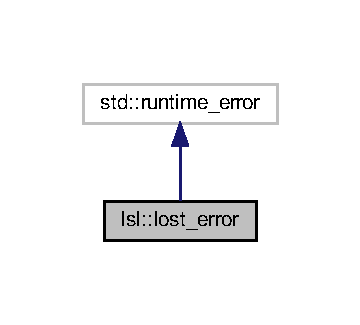
\includegraphics[width=173pt]{d5/d0b/classlsl_1_1lost__error__inherit__graph}
\end{center}
\end{figure}


Collaboration diagram for lsl\+:\+:lost\+\_\+error\+:\nopagebreak
\begin{figure}[H]
\begin{center}
\leavevmode
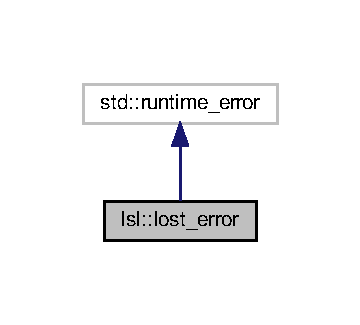
\includegraphics[width=173pt]{d7/d36/classlsl_1_1lost__error__coll__graph}
\end{center}
\end{figure}
\subsection*{Public Member Functions}
\begin{DoxyCompactItemize}
\item 
\mbox{\Hypertarget{classlsl_1_1lost__error_a997ff6ff1ecd4fd33cda631b975d386e}\label{classlsl_1_1lost__error_a997ff6ff1ecd4fd33cda631b975d386e}} 
{\bfseries lost\+\_\+error} (const std\+::string \&msg)
\end{DoxyCompactItemize}


\subsection{Detailed Description}
Exception class that indicates that a stream inlet\textquotesingle{}s source has been irrecoverably lost. 

The documentation for this class was generated from the following file\+:\begin{DoxyCompactItemize}
\item 
include/lsl\+\_\+cpp.\+h\end{DoxyCompactItemize}

\hypertarget{class_ui_1_1_main_window}{}\section{Ui\+:\+:Main\+Window Class Reference}
\label{class_ui_1_1_main_window}\index{Ui\+::\+Main\+Window@{Ui\+::\+Main\+Window}}


{\ttfamily \#include $<$ui\+\_\+mainwindow.\+h$>$}



Inheritance diagram for Ui\+:\+:Main\+Window\+:
\nopagebreak
\begin{figure}[H]
\begin{center}
\leavevmode
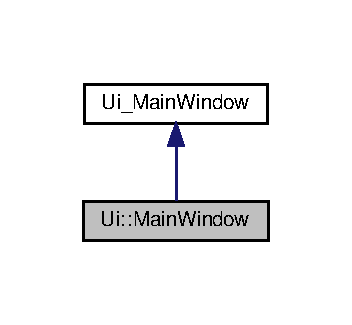
\includegraphics[width=169pt]{d4/de8/class_ui_1_1_main_window__inherit__graph}
\end{center}
\end{figure}


Collaboration diagram for Ui\+:\+:Main\+Window\+:
\nopagebreak
\begin{figure}[H]
\begin{center}
\leavevmode
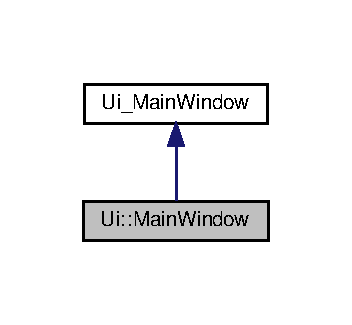
\includegraphics[width=169pt]{dd/dc3/class_ui_1_1_main_window__coll__graph}
\end{center}
\end{figure}
\subsection*{Additional Inherited Members}


The documentation for this class was generated from the following file\+:\begin{DoxyCompactItemize}
\item 
O\+T\+Bconfig\+G\+U\+I/build/\hyperlink{ui__mainwindow_8h}{ui\+\_\+mainwindow.\+h}\end{DoxyCompactItemize}

\hypertarget{class_main_window}{}\section{Main\+Window Class Reference}
\label{class_main_window}\index{Main\+Window@{Main\+Window}}


{\ttfamily \#include $<$mainwindow.\+h$>$}



Inheritance diagram for Main\+Window\+:
\nopagebreak
\begin{figure}[H]
\begin{center}
\leavevmode
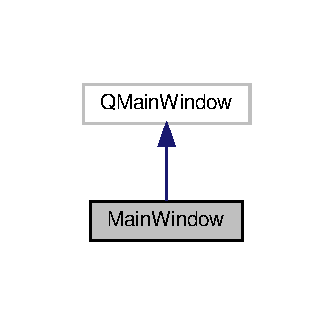
\includegraphics[width=160pt]{de/d4b/class_main_window__inherit__graph}
\end{center}
\end{figure}


Collaboration diagram for Main\+Window\+:
\nopagebreak
\begin{figure}[H]
\begin{center}
\leavevmode
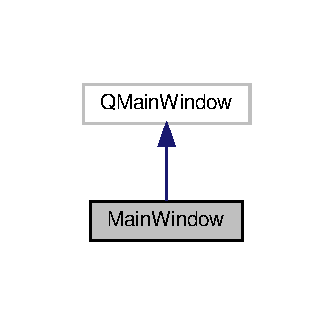
\includegraphics[width=160pt]{d0/db8/class_main_window__coll__graph}
\end{center}
\end{figure}
\subsection*{Public Member Functions}
\begin{DoxyCompactItemize}
\item 
\hyperlink{class_main_window_a996c5a2b6f77944776856f08ec30858d}{Main\+Window} (Q\+Widget $\ast$parent=nullptr)
\item 
\hyperlink{class_main_window_ae98d00a93bc118200eeef9f9bba1dba7}{$\sim$\+Main\+Window} ()
\item 
unsigned char \hyperlink{class_main_window_a86ded1599e8f511ce500bb7a03a5aaf8}{crc} (unsigned char config\mbox{[}$\,$\mbox{]})
\end{DoxyCompactItemize}


\subsection{Constructor \& Destructor Documentation}
\mbox{\Hypertarget{class_main_window_a996c5a2b6f77944776856f08ec30858d}\label{class_main_window_a996c5a2b6f77944776856f08ec30858d}} 
\index{Main\+Window@{Main\+Window}!Main\+Window@{Main\+Window}}
\index{Main\+Window@{Main\+Window}!Main\+Window@{Main\+Window}}
\subsubsection{\texorpdfstring{Main\+Window()}{MainWindow()}}
{\footnotesize\ttfamily Main\+Window\+::\+Main\+Window (\begin{DoxyParamCaption}\item[{Q\+Widget $\ast$}]{parent = {\ttfamily nullptr} }\end{DoxyParamCaption})\hspace{0.3cm}{\ttfamily [explicit]}}

\mbox{\Hypertarget{class_main_window_ae98d00a93bc118200eeef9f9bba1dba7}\label{class_main_window_ae98d00a93bc118200eeef9f9bba1dba7}} 
\index{Main\+Window@{Main\+Window}!````~Main\+Window@{$\sim$\+Main\+Window}}
\index{````~Main\+Window@{$\sim$\+Main\+Window}!Main\+Window@{Main\+Window}}
\subsubsection{\texorpdfstring{$\sim$\+Main\+Window()}{~MainWindow()}}
{\footnotesize\ttfamily Main\+Window\+::$\sim$\+Main\+Window (\begin{DoxyParamCaption}{ }\end{DoxyParamCaption})}



\subsection{Member Function Documentation}
\mbox{\Hypertarget{class_main_window_a86ded1599e8f511ce500bb7a03a5aaf8}\label{class_main_window_a86ded1599e8f511ce500bb7a03a5aaf8}} 
\index{Main\+Window@{Main\+Window}!crc@{crc}}
\index{crc@{crc}!Main\+Window@{Main\+Window}}
\subsubsection{\texorpdfstring{crc()}{crc()}}
{\footnotesize\ttfamily unsigned char Main\+Window\+::crc (\begin{DoxyParamCaption}\item[{unsigned char}]{config\mbox{[}$\,$\mbox{]} }\end{DoxyParamCaption})}



The documentation for this class was generated from the following files\+:\begin{DoxyCompactItemize}
\item 
O\+T\+Bconfig\+G\+U\+I/include/\hyperlink{mainwindow_8h}{mainwindow.\+h}\item 
O\+T\+Bconfig\+G\+U\+I/src/\hyperlink{mainwindow_8cpp}{mainwindow.\+cpp}\end{DoxyCompactItemize}

\hypertarget{structqt__meta__stringdata___main_window__t}{}\section{qt\+\_\+meta\+\_\+stringdata\+\_\+\+Main\+Window\+\_\+t Struct Reference}
\label{structqt__meta__stringdata___main_window__t}\index{qt\+\_\+meta\+\_\+stringdata\+\_\+\+Main\+Window\+\_\+t@{qt\+\_\+meta\+\_\+stringdata\+\_\+\+Main\+Window\+\_\+t}}
\subsection*{Public Attributes}
\begin{DoxyCompactItemize}
\item 
Q\+Byte\+Array\+Data \hyperlink{structqt__meta__stringdata___main_window__t_a70e55b3cae36e81c3bf1093c26a52b51}{data} \mbox{[}7\mbox{]}
\item 
char \hyperlink{structqt__meta__stringdata___main_window__t_a63ac1a7248bae9ea3b1c5c51ac864537}{stringdata0} \mbox{[}75\mbox{]}
\end{DoxyCompactItemize}


\subsection{Member Data Documentation}
\mbox{\Hypertarget{structqt__meta__stringdata___main_window__t_a70e55b3cae36e81c3bf1093c26a52b51}\label{structqt__meta__stringdata___main_window__t_a70e55b3cae36e81c3bf1093c26a52b51}} 
\index{qt\+\_\+meta\+\_\+stringdata\+\_\+\+Main\+Window\+\_\+t@{qt\+\_\+meta\+\_\+stringdata\+\_\+\+Main\+Window\+\_\+t}!data@{data}}
\index{data@{data}!qt\+\_\+meta\+\_\+stringdata\+\_\+\+Main\+Window\+\_\+t@{qt\+\_\+meta\+\_\+stringdata\+\_\+\+Main\+Window\+\_\+t}}
\subsubsection{\texorpdfstring{data}{data}}
{\footnotesize\ttfamily Q\+Byte\+Array\+Data qt\+\_\+meta\+\_\+stringdata\+\_\+\+Main\+Window\+\_\+t\+::data\mbox{[}7\mbox{]}}

\mbox{\Hypertarget{structqt__meta__stringdata___main_window__t_a63ac1a7248bae9ea3b1c5c51ac864537}\label{structqt__meta__stringdata___main_window__t_a63ac1a7248bae9ea3b1c5c51ac864537}} 
\index{qt\+\_\+meta\+\_\+stringdata\+\_\+\+Main\+Window\+\_\+t@{qt\+\_\+meta\+\_\+stringdata\+\_\+\+Main\+Window\+\_\+t}!stringdata0@{stringdata0}}
\index{stringdata0@{stringdata0}!qt\+\_\+meta\+\_\+stringdata\+\_\+\+Main\+Window\+\_\+t@{qt\+\_\+meta\+\_\+stringdata\+\_\+\+Main\+Window\+\_\+t}}
\subsubsection{\texorpdfstring{stringdata0}{stringdata0}}
{\footnotesize\ttfamily char qt\+\_\+meta\+\_\+stringdata\+\_\+\+Main\+Window\+\_\+t\+::stringdata0\mbox{[}75\mbox{]}}



The documentation for this struct was generated from the following file\+:\begin{DoxyCompactItemize}
\item 
O\+T\+Bconfig\+G\+U\+I/build/\hyperlink{moc__mainwindow_8cpp}{moc\+\_\+mainwindow.\+cpp}\end{DoxyCompactItemize}

\hypertarget{classlsl_1_1stream__info}{}\section{lsl\+:\+:stream\+\_\+info Class Reference}
\label{classlsl_1_1stream__info}\index{lsl\+::stream\+\_\+info@{lsl\+::stream\+\_\+info}}


{\ttfamily \#include $<$lsl\+\_\+cpp.\+h$>$}

\subsection*{Public Member Functions}
\begin{DoxyCompactItemize}
\item 
\hyperlink{classlsl_1_1stream__info_a874f4899da89168b768cfe9acdd569a0}{stream\+\_\+info} (const std\+::string \&\hyperlink{classlsl_1_1stream__info_a0862e5c580d65ecf9ceb1fcc26f2ca34}{name}, const std\+::string \&\hyperlink{classlsl_1_1stream__info_a2162830f6867e9513eba9385eb0cbb99}{type}, int32\+\_\+t \hyperlink{classlsl_1_1stream__info_acf09957c1c61a9d9e0f9439037eec305}{channel\+\_\+count}=1, double \hyperlink{classlsl_1_1stream__info_a35b9b9b8947915f9f9518333342e2835}{nominal\+\_\+srate}=\hyperlink{namespacelsl_ac7ebddefe1091ef2d9459b6f9d79f7ab}{I\+R\+R\+E\+G\+U\+L\+A\+R\+\_\+\+R\+A\+TE}, \hyperlink{namespacelsl_a28d50dae6fd82eea8893ce3d63ccd46c}{channel\+\_\+format\+\_\+t} \hyperlink{classlsl_1_1stream__info_aa9695e52570e617d1c7dd4ea9f88b15d}{channel\+\_\+format}=\hyperlink{namespacelsl_a28d50dae6fd82eea8893ce3d63ccd46ca46efa3307b337f7de592753642584616}{cf\+\_\+float32}, const std\+::string \&\hyperlink{classlsl_1_1stream__info_a1f20c68246a88047978d9b03e14a9d2b}{source\+\_\+id}=std\+::string())
\item 
\hyperlink{classlsl_1_1stream__info_a7358ba03d8741b0b194cf9e747405702}{stream\+\_\+info} (\hyperlink{namespacelsl_aa0a9ce9956061679949daa2e35aae2e8}{lsl\+\_\+streaminfo} \hyperlink{classlsl_1_1stream__info_a532f6e8b29052cf11fbf87aeb3424304}{handle})
\item 
std\+::string \hyperlink{classlsl_1_1stream__info_a0862e5c580d65ecf9ceb1fcc26f2ca34}{name} () const
\item 
std\+::string \hyperlink{classlsl_1_1stream__info_a2162830f6867e9513eba9385eb0cbb99}{type} () const
\item 
int32\+\_\+t \hyperlink{classlsl_1_1stream__info_acf09957c1c61a9d9e0f9439037eec305}{channel\+\_\+count} () const
\item 
double \hyperlink{classlsl_1_1stream__info_a35b9b9b8947915f9f9518333342e2835}{nominal\+\_\+srate} () const
\item 
\hyperlink{namespacelsl_a28d50dae6fd82eea8893ce3d63ccd46c}{channel\+\_\+format\+\_\+t} \hyperlink{classlsl_1_1stream__info_aa9695e52570e617d1c7dd4ea9f88b15d}{channel\+\_\+format} () const
\item 
std\+::string \hyperlink{classlsl_1_1stream__info_a1f20c68246a88047978d9b03e14a9d2b}{source\+\_\+id} () const
\item 
int32\+\_\+t \hyperlink{classlsl_1_1stream__info_aabd83f83d0abe8671e766e97f471dea9}{version} () const
\item 
double \hyperlink{classlsl_1_1stream__info_a9a5be16db42c09b1f0cced52a2259db8}{created\+\_\+at} () const
\item 
std\+::string \hyperlink{classlsl_1_1stream__info_ae6fa890ffd440f298dd02fe71eaf3b82}{uid} () const
\item 
std\+::string \hyperlink{classlsl_1_1stream__info_a59036c0e83bcb07b711ec7e3e3b15fef}{session\+\_\+id} () const
\item 
std\+::string \hyperlink{classlsl_1_1stream__info_a52db8d9e073297477d1183dfebe8dcda}{hostname} () const
\item 
\hyperlink{classlsl_1_1xml__element}{xml\+\_\+element} \hyperlink{classlsl_1_1stream__info_a7bbc53bb041757eb87c6c73564981390}{desc} ()
\item 
bool \hyperlink{classlsl_1_1stream__info_a6c3474322d467e8d8198c7a6e4c7ad76}{matches\+\_\+query} (const char $\ast$query) const
\item 
std\+::string \hyperlink{classlsl_1_1stream__info_ab1ccb9c2a1945c7051a0e90edaba8996}{as\+\_\+xml} () const
\item 
int32\+\_\+t \hyperlink{classlsl_1_1stream__info_a7eb192e1913596b017137347e4cc5847}{channel\+\_\+bytes} () const
\begin{DoxyCompactList}\small\item\em Number of bytes occupied by a channel (0 for string-\/typed channels). \end{DoxyCompactList}\item 
int32\+\_\+t \hyperlink{classlsl_1_1stream__info_ab68def3a9c81c289ba46a5b40c6b4084}{sample\+\_\+bytes} () const
\begin{DoxyCompactList}\small\item\em Number of bytes occupied by a sample (0 for string-\/typed channels). \end{DoxyCompactList}\item 
\hyperlink{namespacelsl_aa0a9ce9956061679949daa2e35aae2e8}{lsl\+\_\+streaminfo} \hyperlink{classlsl_1_1stream__info_a532f6e8b29052cf11fbf87aeb3424304}{handle} () const
\begin{DoxyCompactList}\small\item\em Get the implementation handle. \end{DoxyCompactList}\item 
\hyperlink{classlsl_1_1stream__info_a780a9289cc6f1d57215ed297aecfc78b}{stream\+\_\+info} ()
\begin{DoxyCompactList}\small\item\em Default contructor. \end{DoxyCompactList}\item 
\hyperlink{classlsl_1_1stream__info_a82fd071574212a20ba4faffac5ce7803}{stream\+\_\+info} (const \hyperlink{classlsl_1_1stream__info}{stream\+\_\+info} \&rhs)
\begin{DoxyCompactList}\small\item\em Copy constructor. \end{DoxyCompactList}\item 
\hyperlink{classlsl_1_1stream__info}{stream\+\_\+info} \& \hyperlink{classlsl_1_1stream__info_a8ce8011b9da9b90c8e11e5c1c477a0a2}{operator=} (const \hyperlink{classlsl_1_1stream__info}{stream\+\_\+info} \&rhs)
\begin{DoxyCompactList}\small\item\em Assignment operator. \end{DoxyCompactList}\item 
\hyperlink{classlsl_1_1stream__info_afe4bf312984faef204ee4480385a9bc1}{$\sim$stream\+\_\+info} ()
\begin{DoxyCompactList}\small\item\em Destructor. \end{DoxyCompactList}\end{DoxyCompactItemize}
\subsection*{Static Public Member Functions}
\begin{DoxyCompactItemize}
\item 
static \hyperlink{classlsl_1_1stream__info}{stream\+\_\+info} \hyperlink{classlsl_1_1stream__info_abf8fb6ba88d2f6c4069961149f18faec}{from\+\_\+xml} (const std\+::string \&xml)
\begin{DoxyCompactList}\small\item\em Utility function to create a \hyperlink{classlsl_1_1stream__info}{stream\+\_\+info} from an X\+ML representation. \end{DoxyCompactList}\end{DoxyCompactItemize}


\subsection{Constructor \& Destructor Documentation}
\mbox{\Hypertarget{classlsl_1_1stream__info_a874f4899da89168b768cfe9acdd569a0}\label{classlsl_1_1stream__info_a874f4899da89168b768cfe9acdd569a0}} 
\index{lsl\+::stream\+\_\+info@{lsl\+::stream\+\_\+info}!stream\+\_\+info@{stream\+\_\+info}}
\index{stream\+\_\+info@{stream\+\_\+info}!lsl\+::stream\+\_\+info@{lsl\+::stream\+\_\+info}}
\subsubsection{\texorpdfstring{stream\+\_\+info()}{stream\_info()}\hspace{0.1cm}{\footnotesize\ttfamily [1/4]}}
{\footnotesize\ttfamily lsl\+::stream\+\_\+info\+::stream\+\_\+info (\begin{DoxyParamCaption}\item[{const std\+::string \&}]{name,  }\item[{const std\+::string \&}]{type,  }\item[{int32\+\_\+t}]{channel\+\_\+count = {\ttfamily 1},  }\item[{double}]{nominal\+\_\+srate = {\ttfamily \hyperlink{namespacelsl_ac7ebddefe1091ef2d9459b6f9d79f7ab}{I\+R\+R\+E\+G\+U\+L\+A\+R\+\_\+\+R\+A\+TE}},  }\item[{\hyperlink{namespacelsl_a28d50dae6fd82eea8893ce3d63ccd46c}{channel\+\_\+format\+\_\+t}}]{channel\+\_\+format = {\ttfamily \hyperlink{namespacelsl_a28d50dae6fd82eea8893ce3d63ccd46ca46efa3307b337f7de592753642584616}{cf\+\_\+float32}},  }\item[{const std\+::string \&}]{source\+\_\+id = {\ttfamily std\+:\+:string()} }\end{DoxyParamCaption})\hspace{0.3cm}{\ttfamily [inline]}}

Construct a new \hyperlink{classlsl_1_1stream__info}{stream\+\_\+info} object. Core stream information is specified here. Any remaining meta-\/data can be added later. 
\begin{DoxyParams}{Parameters}
{\em name} & Name of the stream. Describes the device (or product series) that this stream makes available (for use by programs, experimenters or data analysts). Cannot be empty. \\
\hline
{\em type} & Content type of the stream. Please see \href{https://github.com/sccn/xdf/wiki/Meta-Data}{\tt https\+://github.\+com/sccn/xdf/wiki/\+Meta-\/\+Data} (or web search for\+: X\+DF meta-\/data) for pre-\/defined content-\/type names, but you can also make up your own. The content type is the preferred way to find streams (as opposed to searching by name). \\
\hline
{\em channel\+\_\+count} & Number of channels per sample. This stays constant for the lifetime of the stream. \\
\hline
{\em nominal\+\_\+srate} & The sampling rate (in Hz) as advertised by the data source, if regular (otherwise set to I\+R\+R\+E\+G\+U\+L\+A\+R\+\_\+\+R\+A\+TE). \\
\hline
{\em channel\+\_\+format} & Format/type of each channel. If your channels have different formats, consider supplying multiple streams or use the largest type that can hold them all (such as cf\+\_\+double64). \\
\hline
{\em source\+\_\+id} & Unique identifier of the device or source of the data, if available (such as the serial number). This is critical for system robustness since it allows recipients to recover from failure even after the serving app, device or computer crashes (just by finding a stream with the same source id on the network again). Therefore, it is highly recommended to always try to provide whatever information can uniquely identify the data source itself. \\
\hline
\end{DoxyParams}
\mbox{\Hypertarget{classlsl_1_1stream__info_a7358ba03d8741b0b194cf9e747405702}\label{classlsl_1_1stream__info_a7358ba03d8741b0b194cf9e747405702}} 
\index{lsl\+::stream\+\_\+info@{lsl\+::stream\+\_\+info}!stream\+\_\+info@{stream\+\_\+info}}
\index{stream\+\_\+info@{stream\+\_\+info}!lsl\+::stream\+\_\+info@{lsl\+::stream\+\_\+info}}
\subsubsection{\texorpdfstring{stream\+\_\+info()}{stream\_info()}\hspace{0.1cm}{\footnotesize\ttfamily [2/4]}}
{\footnotesize\ttfamily lsl\+::stream\+\_\+info\+::stream\+\_\+info (\begin{DoxyParamCaption}\item[{\hyperlink{namespacelsl_aa0a9ce9956061679949daa2e35aae2e8}{lsl\+\_\+streaminfo}}]{handle }\end{DoxyParamCaption})\hspace{0.3cm}{\ttfamily [inline]}}

\mbox{\Hypertarget{classlsl_1_1stream__info_a780a9289cc6f1d57215ed297aecfc78b}\label{classlsl_1_1stream__info_a780a9289cc6f1d57215ed297aecfc78b}} 
\index{lsl\+::stream\+\_\+info@{lsl\+::stream\+\_\+info}!stream\+\_\+info@{stream\+\_\+info}}
\index{stream\+\_\+info@{stream\+\_\+info}!lsl\+::stream\+\_\+info@{lsl\+::stream\+\_\+info}}
\subsubsection{\texorpdfstring{stream\+\_\+info()}{stream\_info()}\hspace{0.1cm}{\footnotesize\ttfamily [3/4]}}
{\footnotesize\ttfamily lsl\+::stream\+\_\+info\+::stream\+\_\+info (\begin{DoxyParamCaption}{ }\end{DoxyParamCaption})\hspace{0.3cm}{\ttfamily [inline]}}



Default contructor. 

\mbox{\Hypertarget{classlsl_1_1stream__info_a82fd071574212a20ba4faffac5ce7803}\label{classlsl_1_1stream__info_a82fd071574212a20ba4faffac5ce7803}} 
\index{lsl\+::stream\+\_\+info@{lsl\+::stream\+\_\+info}!stream\+\_\+info@{stream\+\_\+info}}
\index{stream\+\_\+info@{stream\+\_\+info}!lsl\+::stream\+\_\+info@{lsl\+::stream\+\_\+info}}
\subsubsection{\texorpdfstring{stream\+\_\+info()}{stream\_info()}\hspace{0.1cm}{\footnotesize\ttfamily [4/4]}}
{\footnotesize\ttfamily lsl\+::stream\+\_\+info\+::stream\+\_\+info (\begin{DoxyParamCaption}\item[{const \hyperlink{classlsl_1_1stream__info}{stream\+\_\+info} \&}]{rhs }\end{DoxyParamCaption})\hspace{0.3cm}{\ttfamily [inline]}}



Copy constructor. 

\mbox{\Hypertarget{classlsl_1_1stream__info_afe4bf312984faef204ee4480385a9bc1}\label{classlsl_1_1stream__info_afe4bf312984faef204ee4480385a9bc1}} 
\index{lsl\+::stream\+\_\+info@{lsl\+::stream\+\_\+info}!````~stream\+\_\+info@{$\sim$stream\+\_\+info}}
\index{````~stream\+\_\+info@{$\sim$stream\+\_\+info}!lsl\+::stream\+\_\+info@{lsl\+::stream\+\_\+info}}
\subsubsection{\texorpdfstring{$\sim$stream\+\_\+info()}{~stream\_info()}}
{\footnotesize\ttfamily lsl\+::stream\+\_\+info\+::$\sim$stream\+\_\+info (\begin{DoxyParamCaption}{ }\end{DoxyParamCaption})\hspace{0.3cm}{\ttfamily [inline]}}



Destructor. 



\subsection{Member Function Documentation}
\mbox{\Hypertarget{classlsl_1_1stream__info_ab1ccb9c2a1945c7051a0e90edaba8996}\label{classlsl_1_1stream__info_ab1ccb9c2a1945c7051a0e90edaba8996}} 
\index{lsl\+::stream\+\_\+info@{lsl\+::stream\+\_\+info}!as\+\_\+xml@{as\+\_\+xml}}
\index{as\+\_\+xml@{as\+\_\+xml}!lsl\+::stream\+\_\+info@{lsl\+::stream\+\_\+info}}
\subsubsection{\texorpdfstring{as\+\_\+xml()}{as\_xml()}}
{\footnotesize\ttfamily std\+::string lsl\+::stream\+\_\+info\+::as\+\_\+xml (\begin{DoxyParamCaption}{ }\end{DoxyParamCaption}) const\hspace{0.3cm}{\ttfamily [inline]}}

Retrieve the entire \hyperlink{classlsl_1_1stream__info}{stream\+\_\+info} in X\+ML format. This yields an X\+ML document (in string form) whose top-\/level element is $<$info$>$. The info element contains one element for each field of the \hyperlink{classlsl_1_1stream__info}{stream\+\_\+info} class, including\+: a) the core elements $<$name$>$, $<$type$>$, $<$channel\+\_\+count$>$, $<$nominal\+\_\+srate$>$, $<$channel\+\_\+format$>$, $<$source\+\_\+id$>$ b) the misc elements $<$version$>$, $<$created\+\_\+at$>$, $<$uid$>$, $<$session\+\_\+id$>$, $<$v4address$>$, $<$v4data\+\_\+port$>$, $<$v4service\+\_\+port$>$, $<$v6address$>$, $<$v6data\+\_\+port$>$, $<$v6service\+\_\+port$>$ c) the extended description element $<$desc$>$ with user-\/defined sub-\/elements. \mbox{\Hypertarget{classlsl_1_1stream__info_a7eb192e1913596b017137347e4cc5847}\label{classlsl_1_1stream__info_a7eb192e1913596b017137347e4cc5847}} 
\index{lsl\+::stream\+\_\+info@{lsl\+::stream\+\_\+info}!channel\+\_\+bytes@{channel\+\_\+bytes}}
\index{channel\+\_\+bytes@{channel\+\_\+bytes}!lsl\+::stream\+\_\+info@{lsl\+::stream\+\_\+info}}
\subsubsection{\texorpdfstring{channel\+\_\+bytes()}{channel\_bytes()}}
{\footnotesize\ttfamily int32\+\_\+t lsl\+::stream\+\_\+info\+::channel\+\_\+bytes (\begin{DoxyParamCaption}{ }\end{DoxyParamCaption}) const\hspace{0.3cm}{\ttfamily [inline]}}



Number of bytes occupied by a channel (0 for string-\/typed channels). 

\mbox{\Hypertarget{classlsl_1_1stream__info_acf09957c1c61a9d9e0f9439037eec305}\label{classlsl_1_1stream__info_acf09957c1c61a9d9e0f9439037eec305}} 
\index{lsl\+::stream\+\_\+info@{lsl\+::stream\+\_\+info}!channel\+\_\+count@{channel\+\_\+count}}
\index{channel\+\_\+count@{channel\+\_\+count}!lsl\+::stream\+\_\+info@{lsl\+::stream\+\_\+info}}
\subsubsection{\texorpdfstring{channel\+\_\+count()}{channel\_count()}}
{\footnotesize\ttfamily int32\+\_\+t lsl\+::stream\+\_\+info\+::channel\+\_\+count (\begin{DoxyParamCaption}{ }\end{DoxyParamCaption}) const\hspace{0.3cm}{\ttfamily [inline]}}

Number of channels of the stream. A stream has at least one channel; the channel count stays constant for all samples. \mbox{\Hypertarget{classlsl_1_1stream__info_aa9695e52570e617d1c7dd4ea9f88b15d}\label{classlsl_1_1stream__info_aa9695e52570e617d1c7dd4ea9f88b15d}} 
\index{lsl\+::stream\+\_\+info@{lsl\+::stream\+\_\+info}!channel\+\_\+format@{channel\+\_\+format}}
\index{channel\+\_\+format@{channel\+\_\+format}!lsl\+::stream\+\_\+info@{lsl\+::stream\+\_\+info}}
\subsubsection{\texorpdfstring{channel\+\_\+format()}{channel\_format()}}
{\footnotesize\ttfamily \hyperlink{namespacelsl_a28d50dae6fd82eea8893ce3d63ccd46c}{channel\+\_\+format\+\_\+t} lsl\+::stream\+\_\+info\+::channel\+\_\+format (\begin{DoxyParamCaption}{ }\end{DoxyParamCaption}) const\hspace{0.3cm}{\ttfamily [inline]}}

Channel format of the stream. All channels in a stream have the same format. However, a device might offer multiple time-\/synched streams each with its own format. \mbox{\Hypertarget{classlsl_1_1stream__info_a9a5be16db42c09b1f0cced52a2259db8}\label{classlsl_1_1stream__info_a9a5be16db42c09b1f0cced52a2259db8}} 
\index{lsl\+::stream\+\_\+info@{lsl\+::stream\+\_\+info}!created\+\_\+at@{created\+\_\+at}}
\index{created\+\_\+at@{created\+\_\+at}!lsl\+::stream\+\_\+info@{lsl\+::stream\+\_\+info}}
\subsubsection{\texorpdfstring{created\+\_\+at()}{created\_at()}}
{\footnotesize\ttfamily double lsl\+::stream\+\_\+info\+::created\+\_\+at (\begin{DoxyParamCaption}{ }\end{DoxyParamCaption}) const\hspace{0.3cm}{\ttfamily [inline]}}

Creation time stamp of the stream. This is the time stamp when the stream was first created (as determined via \hyperlink{namespacelsl_ae1766ae2ab66141cb927612e57a0c8c6}{local\+\_\+clock()} on the providing machine). \mbox{\Hypertarget{classlsl_1_1stream__info_a7bbc53bb041757eb87c6c73564981390}\label{classlsl_1_1stream__info_a7bbc53bb041757eb87c6c73564981390}} 
\index{lsl\+::stream\+\_\+info@{lsl\+::stream\+\_\+info}!desc@{desc}}
\index{desc@{desc}!lsl\+::stream\+\_\+info@{lsl\+::stream\+\_\+info}}
\subsubsection{\texorpdfstring{desc()}{desc()}}
{\footnotesize\ttfamily \hyperlink{classlsl_1_1xml__element}{xml\+\_\+element} lsl\+::stream\+\_\+info\+::desc (\begin{DoxyParamCaption}{ }\end{DoxyParamCaption})\hspace{0.3cm}{\ttfamily [inline]}}

Extended description of the stream. It is highly recommended that at least the channel labels are described here. See code examples on the L\+SL wiki. Other information, such as amplifier settings, measurement units if deviating from defaults, setup information, subject information, etc., can be specified here, as well. Meta-\/data recommendations follow the X\+DF file format project (github.\+com/sccn/xdf/wiki/\+Meta-\/\+Data or web search for\+: X\+DF meta-\/data).

Important\+: if you use a stream content type for which meta-\/data recommendations exist, please try to lay out your meta-\/data in agreement with these recommendations for compatibility with other applications. \mbox{\Hypertarget{classlsl_1_1stream__info_abf8fb6ba88d2f6c4069961149f18faec}\label{classlsl_1_1stream__info_abf8fb6ba88d2f6c4069961149f18faec}} 
\index{lsl\+::stream\+\_\+info@{lsl\+::stream\+\_\+info}!from\+\_\+xml@{from\+\_\+xml}}
\index{from\+\_\+xml@{from\+\_\+xml}!lsl\+::stream\+\_\+info@{lsl\+::stream\+\_\+info}}
\subsubsection{\texorpdfstring{from\+\_\+xml()}{from\_xml()}}
{\footnotesize\ttfamily static \hyperlink{classlsl_1_1stream__info}{stream\+\_\+info} lsl\+::stream\+\_\+info\+::from\+\_\+xml (\begin{DoxyParamCaption}\item[{const std\+::string \&}]{xml }\end{DoxyParamCaption})\hspace{0.3cm}{\ttfamily [inline]}, {\ttfamily [static]}}



Utility function to create a \hyperlink{classlsl_1_1stream__info}{stream\+\_\+info} from an X\+ML representation. 

\mbox{\Hypertarget{classlsl_1_1stream__info_a532f6e8b29052cf11fbf87aeb3424304}\label{classlsl_1_1stream__info_a532f6e8b29052cf11fbf87aeb3424304}} 
\index{lsl\+::stream\+\_\+info@{lsl\+::stream\+\_\+info}!handle@{handle}}
\index{handle@{handle}!lsl\+::stream\+\_\+info@{lsl\+::stream\+\_\+info}}
\subsubsection{\texorpdfstring{handle()}{handle()}}
{\footnotesize\ttfamily \hyperlink{namespacelsl_aa0a9ce9956061679949daa2e35aae2e8}{lsl\+\_\+streaminfo} lsl\+::stream\+\_\+info\+::handle (\begin{DoxyParamCaption}{ }\end{DoxyParamCaption}) const\hspace{0.3cm}{\ttfamily [inline]}}



Get the implementation handle. 

\mbox{\Hypertarget{classlsl_1_1stream__info_a52db8d9e073297477d1183dfebe8dcda}\label{classlsl_1_1stream__info_a52db8d9e073297477d1183dfebe8dcda}} 
\index{lsl\+::stream\+\_\+info@{lsl\+::stream\+\_\+info}!hostname@{hostname}}
\index{hostname@{hostname}!lsl\+::stream\+\_\+info@{lsl\+::stream\+\_\+info}}
\subsubsection{\texorpdfstring{hostname()}{hostname()}}
{\footnotesize\ttfamily std\+::string lsl\+::stream\+\_\+info\+::hostname (\begin{DoxyParamCaption}{ }\end{DoxyParamCaption}) const\hspace{0.3cm}{\ttfamily [inline]}}

Hostname of the providing machine. \mbox{\Hypertarget{classlsl_1_1stream__info_a6c3474322d467e8d8198c7a6e4c7ad76}\label{classlsl_1_1stream__info_a6c3474322d467e8d8198c7a6e4c7ad76}} 
\index{lsl\+::stream\+\_\+info@{lsl\+::stream\+\_\+info}!matches\+\_\+query@{matches\+\_\+query}}
\index{matches\+\_\+query@{matches\+\_\+query}!lsl\+::stream\+\_\+info@{lsl\+::stream\+\_\+info}}
\subsubsection{\texorpdfstring{matches\+\_\+query()}{matches\_query()}}
{\footnotesize\ttfamily bool lsl\+::stream\+\_\+info\+::matches\+\_\+query (\begin{DoxyParamCaption}\item[{const char $\ast$}]{query }\end{DoxyParamCaption}) const\hspace{0.3cm}{\ttfamily [inline]}}





Tries to match the stream info X\+ML element {\ttfamily info} against an \href{https://en.wikipedia.org/wiki/XPath#Syntax_and_semantics_(XPath_1.0)}{\tt X\+Path} query.

Example query strings\+: 
\begin{DoxyCode}
\hyperlink{classlsl_1_1stream__info_acf09957c1c61a9d9e0f9439037eec305}{channel\_count}>5 and type=\textcolor{stringliteral}{'EEG'}
type=\textcolor{stringliteral}{'TestStream'} or contains(\hyperlink{classlsl_1_1stream__info_a0862e5c580d65ecf9ceb1fcc26f2ca34}{name},\textcolor{stringliteral}{'Brain'})
\hyperlink{classlsl_1_1stream__info_a0862e5c580d65ecf9ceb1fcc26f2ca34}{name}='ExampleStream'
\end{DoxyCode}
 \mbox{\Hypertarget{classlsl_1_1stream__info_a0862e5c580d65ecf9ceb1fcc26f2ca34}\label{classlsl_1_1stream__info_a0862e5c580d65ecf9ceb1fcc26f2ca34}} 
\index{lsl\+::stream\+\_\+info@{lsl\+::stream\+\_\+info}!name@{name}}
\index{name@{name}!lsl\+::stream\+\_\+info@{lsl\+::stream\+\_\+info}}
\subsubsection{\texorpdfstring{name()}{name()}}
{\footnotesize\ttfamily std\+::string lsl\+::stream\+\_\+info\+::name (\begin{DoxyParamCaption}{ }\end{DoxyParamCaption}) const\hspace{0.3cm}{\ttfamily [inline]}}

Name of the stream. This is a human-\/readable name. For streams offered by device modules, it refers to the type of device or product series that is generating the data of the stream. If the source is an application, the name may be a more generic or specific identifier. Multiple streams with the same name can coexist, though potentially at the cost of ambiguity (for the recording app or experimenter). \mbox{\Hypertarget{classlsl_1_1stream__info_a35b9b9b8947915f9f9518333342e2835}\label{classlsl_1_1stream__info_a35b9b9b8947915f9f9518333342e2835}} 
\index{lsl\+::stream\+\_\+info@{lsl\+::stream\+\_\+info}!nominal\+\_\+srate@{nominal\+\_\+srate}}
\index{nominal\+\_\+srate@{nominal\+\_\+srate}!lsl\+::stream\+\_\+info@{lsl\+::stream\+\_\+info}}
\subsubsection{\texorpdfstring{nominal\+\_\+srate()}{nominal\_srate()}}
{\footnotesize\ttfamily double lsl\+::stream\+\_\+info\+::nominal\+\_\+srate (\begin{DoxyParamCaption}{ }\end{DoxyParamCaption}) const\hspace{0.3cm}{\ttfamily [inline]}}

Sampling rate of the stream, according to the source (in Hz). If a stream is irregularly sampled, this should be set to I\+R\+R\+E\+G\+U\+L\+A\+R\+\_\+\+R\+A\+TE.

Note that no data will be lost even if this sampling rate is incorrect or if a device has temporary hiccups, since all samples will be recorded anyway (except for those dropped by the device itself). However, when the recording is imported into an application, a good importer may correct such errors more accurately if the advertised sampling rate was close to the specs of the device. \mbox{\Hypertarget{classlsl_1_1stream__info_a8ce8011b9da9b90c8e11e5c1c477a0a2}\label{classlsl_1_1stream__info_a8ce8011b9da9b90c8e11e5c1c477a0a2}} 
\index{lsl\+::stream\+\_\+info@{lsl\+::stream\+\_\+info}!operator=@{operator=}}
\index{operator=@{operator=}!lsl\+::stream\+\_\+info@{lsl\+::stream\+\_\+info}}
\subsubsection{\texorpdfstring{operator=()}{operator=()}}
{\footnotesize\ttfamily \hyperlink{classlsl_1_1stream__info}{stream\+\_\+info}\& lsl\+::stream\+\_\+info\+::operator= (\begin{DoxyParamCaption}\item[{const \hyperlink{classlsl_1_1stream__info}{stream\+\_\+info} \&}]{rhs }\end{DoxyParamCaption})\hspace{0.3cm}{\ttfamily [inline]}}



Assignment operator. 

\mbox{\Hypertarget{classlsl_1_1stream__info_ab68def3a9c81c289ba46a5b40c6b4084}\label{classlsl_1_1stream__info_ab68def3a9c81c289ba46a5b40c6b4084}} 
\index{lsl\+::stream\+\_\+info@{lsl\+::stream\+\_\+info}!sample\+\_\+bytes@{sample\+\_\+bytes}}
\index{sample\+\_\+bytes@{sample\+\_\+bytes}!lsl\+::stream\+\_\+info@{lsl\+::stream\+\_\+info}}
\subsubsection{\texorpdfstring{sample\+\_\+bytes()}{sample\_bytes()}}
{\footnotesize\ttfamily int32\+\_\+t lsl\+::stream\+\_\+info\+::sample\+\_\+bytes (\begin{DoxyParamCaption}{ }\end{DoxyParamCaption}) const\hspace{0.3cm}{\ttfamily [inline]}}



Number of bytes occupied by a sample (0 for string-\/typed channels). 

\mbox{\Hypertarget{classlsl_1_1stream__info_a59036c0e83bcb07b711ec7e3e3b15fef}\label{classlsl_1_1stream__info_a59036c0e83bcb07b711ec7e3e3b15fef}} 
\index{lsl\+::stream\+\_\+info@{lsl\+::stream\+\_\+info}!session\+\_\+id@{session\+\_\+id}}
\index{session\+\_\+id@{session\+\_\+id}!lsl\+::stream\+\_\+info@{lsl\+::stream\+\_\+info}}
\subsubsection{\texorpdfstring{session\+\_\+id()}{session\_id()}}
{\footnotesize\ttfamily std\+::string lsl\+::stream\+\_\+info\+::session\+\_\+id (\begin{DoxyParamCaption}{ }\end{DoxyParamCaption}) const\hspace{0.3cm}{\ttfamily [inline]}}

Session ID for the given stream. The session id is an optional human-\/assigned identifier of the recording session. While it is rarely used, it can be used to prevent concurrent recording activitites on the same sub-\/network (e.\+g., in multiple experiment areas) from seeing each other\textquotesingle{}s streams (assigned via a configuration file by the experimenter, see Network Connectivity in the L\+SL wiki). \mbox{\Hypertarget{classlsl_1_1stream__info_a1f20c68246a88047978d9b03e14a9d2b}\label{classlsl_1_1stream__info_a1f20c68246a88047978d9b03e14a9d2b}} 
\index{lsl\+::stream\+\_\+info@{lsl\+::stream\+\_\+info}!source\+\_\+id@{source\+\_\+id}}
\index{source\+\_\+id@{source\+\_\+id}!lsl\+::stream\+\_\+info@{lsl\+::stream\+\_\+info}}
\subsubsection{\texorpdfstring{source\+\_\+id()}{source\_id()}}
{\footnotesize\ttfamily std\+::string lsl\+::stream\+\_\+info\+::source\+\_\+id (\begin{DoxyParamCaption}{ }\end{DoxyParamCaption}) const\hspace{0.3cm}{\ttfamily [inline]}}

Unique identifier of the stream\textquotesingle{}s source, if available. The unique source (or device) identifier is an optional piece of information that, if available, allows that endpoints (such as the recording program) can re-\/acquire a stream automatically once it is back online. \mbox{\Hypertarget{classlsl_1_1stream__info_a2162830f6867e9513eba9385eb0cbb99}\label{classlsl_1_1stream__info_a2162830f6867e9513eba9385eb0cbb99}} 
\index{lsl\+::stream\+\_\+info@{lsl\+::stream\+\_\+info}!type@{type}}
\index{type@{type}!lsl\+::stream\+\_\+info@{lsl\+::stream\+\_\+info}}
\subsubsection{\texorpdfstring{type()}{type()}}
{\footnotesize\ttfamily std\+::string lsl\+::stream\+\_\+info\+::type (\begin{DoxyParamCaption}{ }\end{DoxyParamCaption}) const\hspace{0.3cm}{\ttfamily [inline]}}

Content type of the stream. The content type is a short string such as \char`\"{}\+E\+E\+G\char`\"{}, \char`\"{}\+Gaze\char`\"{} which describes the content carried by the channel (if known). If a stream contains mixed content this value need not be assigned but may instead be stored in the description of channel types. To be useful to applications and automated processing systems using the recommended content types is preferred. Content types usually follow those pre-\/defined in \href{https://github.com/sccn/xdf/wiki/Meta-Data}{\tt https\+://github.\+com/sccn/xdf/wiki/\+Meta-\/\+Data} (or web search for\+: X\+DF meta-\/data). \mbox{\Hypertarget{classlsl_1_1stream__info_ae6fa890ffd440f298dd02fe71eaf3b82}\label{classlsl_1_1stream__info_ae6fa890ffd440f298dd02fe71eaf3b82}} 
\index{lsl\+::stream\+\_\+info@{lsl\+::stream\+\_\+info}!uid@{uid}}
\index{uid@{uid}!lsl\+::stream\+\_\+info@{lsl\+::stream\+\_\+info}}
\subsubsection{\texorpdfstring{uid()}{uid()}}
{\footnotesize\ttfamily std\+::string lsl\+::stream\+\_\+info\+::uid (\begin{DoxyParamCaption}{ }\end{DoxyParamCaption}) const\hspace{0.3cm}{\ttfamily [inline]}}

Unique ID of the stream outlet instance (once assigned). This is a unique identifier of the stream outlet, and is guaranteed to be different across multiple instantiations of the same outlet (e.\+g., after a re-\/start). \mbox{\Hypertarget{classlsl_1_1stream__info_aabd83f83d0abe8671e766e97f471dea9}\label{classlsl_1_1stream__info_aabd83f83d0abe8671e766e97f471dea9}} 
\index{lsl\+::stream\+\_\+info@{lsl\+::stream\+\_\+info}!version@{version}}
\index{version@{version}!lsl\+::stream\+\_\+info@{lsl\+::stream\+\_\+info}}
\subsubsection{\texorpdfstring{version()}{version()}}
{\footnotesize\ttfamily int32\+\_\+t lsl\+::stream\+\_\+info\+::version (\begin{DoxyParamCaption}{ }\end{DoxyParamCaption}) const\hspace{0.3cm}{\ttfamily [inline]}}

Protocol version used to deliver the stream. 

The documentation for this class was generated from the following file\+:\begin{DoxyCompactItemize}
\item 
include/\hyperlink{lsl__cpp_8h}{lsl\+\_\+cpp.\+h}\end{DoxyCompactItemize}

\hypertarget{classlsl_1_1stream__inlet}{}\section{lsl\+:\+:stream\+\_\+inlet Class Reference}
\label{classlsl_1_1stream__inlet}\index{lsl\+::stream\+\_\+inlet@{lsl\+::stream\+\_\+inlet}}


{\ttfamily \#include $<$lsl\+\_\+cpp.\+h$>$}

\subsection*{Public Member Functions}
\begin{DoxyCompactItemize}
\item 
\hyperlink{classlsl_1_1stream__inlet_a7c93b7d4fc053b2e3320841371b32919}{stream\+\_\+inlet} (const \hyperlink{classlsl_1_1stream__info}{stream\+\_\+info} \&\hyperlink{classlsl_1_1stream__inlet_ae895a8d5c10dc4072e969686fc402b5b}{info}, int32\+\_\+t max\+\_\+buflen=360, int32\+\_\+t max\+\_\+chunklen=0, bool recover=true)
\item 
\hyperlink{classlsl_1_1stream__inlet_ac3b37a1c2e376280c3144f422bb27d79}{$\sim$stream\+\_\+inlet} ()
\item 
\hyperlink{classlsl_1_1stream__info}{stream\+\_\+info} \hyperlink{classlsl_1_1stream__inlet_ae895a8d5c10dc4072e969686fc402b5b}{info} (double timeout=\hyperlink{namespacelsl_a74cfbc9077aca21295117217249721ed}{F\+O\+R\+E\+V\+ER})
\item 
void \hyperlink{classlsl_1_1stream__inlet_ad84029ed0662d755b0544c7652348718}{open\+\_\+stream} (double timeout=\hyperlink{namespacelsl_a74cfbc9077aca21295117217249721ed}{F\+O\+R\+E\+V\+ER})
\item 
void \hyperlink{classlsl_1_1stream__inlet_a77c2f10ed843723c7473aa52dcf544a0}{close\+\_\+stream} ()
\item 
double \hyperlink{classlsl_1_1stream__inlet_a845d95f5fc60fb9cd01fb73d3da75e94}{time\+\_\+correction} (double timeout=\hyperlink{namespacelsl_a74cfbc9077aca21295117217249721ed}{F\+O\+R\+E\+V\+ER})
\item 
double \hyperlink{classlsl_1_1stream__inlet_a9603f3365093f43f9e2bae1b9e9b2cd8}{time\+\_\+correction} (double $\ast$remote\+\_\+time, double $\ast$uncertainty, double timeout=\hyperlink{namespacelsl_a74cfbc9077aca21295117217249721ed}{F\+O\+R\+E\+V\+ER})
\item 
void \hyperlink{classlsl_1_1stream__inlet_aaf40ba9c127a1828933613d0f2b0fc3d}{set\+\_\+postprocessing} (uint32\+\_\+t flags=\hyperlink{namespacelsl_aaa1cffa7d29bb2756522bc2bb069e310a198f16659e71b850e4674ed31d10e914}{post\+\_\+\+A\+LL})
\item 
{\footnotesize template$<$class T , int N$>$ }\\double \hyperlink{classlsl_1_1stream__inlet_a58dc91be6ec0d1b83024a169ad0c292b}{pull\+\_\+sample} (T sample\mbox{[}N\mbox{]}, double timeout=\hyperlink{namespacelsl_a74cfbc9077aca21295117217249721ed}{F\+O\+R\+E\+V\+ER})
\item 
double \hyperlink{classlsl_1_1stream__inlet_af3707fbfd5e9f54be73f9d55de55a8fc}{pull\+\_\+sample} (std\+::vector$<$ float $>$ \&sample, double timeout=\hyperlink{namespacelsl_a74cfbc9077aca21295117217249721ed}{F\+O\+R\+E\+V\+ER})
\item 
double \hyperlink{classlsl_1_1stream__inlet_a447dd270fa83d8f1df16963b8601027e}{pull\+\_\+sample} (std\+::vector$<$ double $>$ \&sample, double timeout=\hyperlink{namespacelsl_a74cfbc9077aca21295117217249721ed}{F\+O\+R\+E\+V\+ER})
\item 
double \hyperlink{classlsl_1_1stream__inlet_a80fecf88ba609c7e4898eb16a49f2b75}{pull\+\_\+sample} (std\+::vector$<$ long $>$ \&sample, double timeout=\hyperlink{namespacelsl_a74cfbc9077aca21295117217249721ed}{F\+O\+R\+E\+V\+ER})
\item 
double \hyperlink{classlsl_1_1stream__inlet_af33558ccbbe57767386278d2255db1a1}{pull\+\_\+sample} (std\+::vector$<$ int32\+\_\+t $>$ \&sample, double timeout=\hyperlink{namespacelsl_a74cfbc9077aca21295117217249721ed}{F\+O\+R\+E\+V\+ER})
\item 
double \hyperlink{classlsl_1_1stream__inlet_a7789d75e1afceaf5187e8bc33a0b99be}{pull\+\_\+sample} (std\+::vector$<$ int16\+\_\+t $>$ \&sample, double timeout=\hyperlink{namespacelsl_a74cfbc9077aca21295117217249721ed}{F\+O\+R\+E\+V\+ER})
\item 
double \hyperlink{classlsl_1_1stream__inlet_a3a2a662e0b723d7f2101b79eb08371b7}{pull\+\_\+sample} (std\+::vector$<$ char $>$ \&sample, double timeout=\hyperlink{namespacelsl_a74cfbc9077aca21295117217249721ed}{F\+O\+R\+E\+V\+ER})
\item 
double \hyperlink{classlsl_1_1stream__inlet_a78a36bf33ddfc7101bd15cb5bcb9561d}{pull\+\_\+sample} (std\+::vector$<$ std\+::string $>$ \&sample, double timeout=\hyperlink{namespacelsl_a74cfbc9077aca21295117217249721ed}{F\+O\+R\+E\+V\+ER})
\item 
double \hyperlink{classlsl_1_1stream__inlet_a4a10bd640a10c317ba4a0244cc986146}{pull\+\_\+sample} (float $\ast$buffer, int32\+\_\+t buffer\+\_\+elements, double timeout=\hyperlink{namespacelsl_a74cfbc9077aca21295117217249721ed}{F\+O\+R\+E\+V\+ER})
\item 
double \hyperlink{classlsl_1_1stream__inlet_acb78fe666a3be090278bc3d1f3eb7619}{pull\+\_\+sample} (double $\ast$buffer, int32\+\_\+t buffer\+\_\+elements, double timeout=\hyperlink{namespacelsl_a74cfbc9077aca21295117217249721ed}{F\+O\+R\+E\+V\+ER})
\item 
double \hyperlink{classlsl_1_1stream__inlet_a774c17a647ebd321b5ce4a5450f71202}{pull\+\_\+sample} (long $\ast$buffer, int32\+\_\+t buffer\+\_\+elements, double timeout=\hyperlink{namespacelsl_a74cfbc9077aca21295117217249721ed}{F\+O\+R\+E\+V\+ER})
\item 
double \hyperlink{classlsl_1_1stream__inlet_ae4534102453ccd98f319c746ec1de0a9}{pull\+\_\+sample} (int32\+\_\+t $\ast$buffer, int32\+\_\+t buffer\+\_\+elements, double timeout=\hyperlink{namespacelsl_a74cfbc9077aca21295117217249721ed}{F\+O\+R\+E\+V\+ER})
\item 
double \hyperlink{classlsl_1_1stream__inlet_a3462f2634ce13e7f9c764e16a58a71a6}{pull\+\_\+sample} (int16\+\_\+t $\ast$buffer, int32\+\_\+t buffer\+\_\+elements, double timeout=\hyperlink{namespacelsl_a74cfbc9077aca21295117217249721ed}{F\+O\+R\+E\+V\+ER})
\item 
double \hyperlink{classlsl_1_1stream__inlet_a9183e81a122df862eff9ea9797c82b73}{pull\+\_\+sample} (char $\ast$buffer, int32\+\_\+t buffer\+\_\+elements, double timeout=\hyperlink{namespacelsl_a74cfbc9077aca21295117217249721ed}{F\+O\+R\+E\+V\+ER})
\item 
double \hyperlink{classlsl_1_1stream__inlet_a52e95747438991868e3eb9c791e24f42}{pull\+\_\+sample} (std\+::string $\ast$buffer, int32\+\_\+t buffer\+\_\+elements, double timeout=\hyperlink{namespacelsl_a74cfbc9077aca21295117217249721ed}{F\+O\+R\+E\+V\+ER})
\item 
{\footnotesize template$<$class T $>$ }\\double \hyperlink{classlsl_1_1stream__inlet_a540c7ba2c23188916ffe311c26c2c081}{pull\+\_\+numeric\+\_\+struct} (T \&sample, double timeout=\hyperlink{namespacelsl_a74cfbc9077aca21295117217249721ed}{F\+O\+R\+E\+V\+ER})
\item 
double \hyperlink{classlsl_1_1stream__inlet_ae8f7beaaa82d192d844abdd1531f6b9a}{pull\+\_\+numeric\+\_\+raw} (void $\ast$sample, int32\+\_\+t buffer\+\_\+bytes, double timeout=\hyperlink{namespacelsl_a74cfbc9077aca21295117217249721ed}{F\+O\+R\+E\+V\+ER})
\item 
{\footnotesize template$<$class T $>$ }\\bool \hyperlink{classlsl_1_1stream__inlet_af9051121db6ffa6945bd2288b2bf2a15}{pull\+\_\+chunk} (std\+::vector$<$ std\+::vector$<$ T $>$ $>$ \&chunk, std\+::vector$<$ double $>$ \&timestamps)
\item 
{\footnotesize template$<$class T $>$ }\\double \hyperlink{classlsl_1_1stream__inlet_acf6cdc3afdbb4c31c97fb979e4aca632}{pull\+\_\+chunk} (std\+::vector$<$ std\+::vector$<$ T $>$ $>$ \&chunk)
\item 
{\footnotesize template$<$class T $>$ }\\std\+::vector$<$ std\+::vector$<$ T $>$ $>$ \hyperlink{classlsl_1_1stream__inlet_a558f53812f5dc3c19b2cbe0026a61f6a}{pull\+\_\+chunk} ()
\item 
std\+::size\+\_\+t \hyperlink{classlsl_1_1stream__inlet_a97adf2cb7d60e4b47bf25217a2b17964}{pull\+\_\+chunk\+\_\+multiplexed} (float $\ast$data\+\_\+buffer, double $\ast$timestamp\+\_\+buffer, std\+::size\+\_\+t data\+\_\+buffer\+\_\+elements, std\+::size\+\_\+t timestamp\+\_\+buffer\+\_\+elements, double timeout=0.\+0)
\item 
std\+::size\+\_\+t \hyperlink{classlsl_1_1stream__inlet_abdb890fbad785ed4bc39288fc2f47329}{pull\+\_\+chunk\+\_\+multiplexed} (double $\ast$data\+\_\+buffer, double $\ast$timestamp\+\_\+buffer, std\+::size\+\_\+t data\+\_\+buffer\+\_\+elements, std\+::size\+\_\+t timestamp\+\_\+buffer\+\_\+elements, double timeout=0.\+0)
\item 
std\+::size\+\_\+t \hyperlink{classlsl_1_1stream__inlet_aa2f2c576a6b5a3bf562878200829bb47}{pull\+\_\+chunk\+\_\+multiplexed} (long $\ast$data\+\_\+buffer, double $\ast$timestamp\+\_\+buffer, std\+::size\+\_\+t data\+\_\+buffer\+\_\+elements, std\+::size\+\_\+t timestamp\+\_\+buffer\+\_\+elements, double timeout=0.\+0)
\item 
std\+::size\+\_\+t \hyperlink{classlsl_1_1stream__inlet_a3b93d803b348905bc34747c5820d6364}{pull\+\_\+chunk\+\_\+multiplexed} (int32\+\_\+t $\ast$data\+\_\+buffer, double $\ast$timestamp\+\_\+buffer, std\+::size\+\_\+t data\+\_\+buffer\+\_\+elements, std\+::size\+\_\+t timestamp\+\_\+buffer\+\_\+elements, double timeout=0.\+0)
\item 
std\+::size\+\_\+t \hyperlink{classlsl_1_1stream__inlet_a40e9727b155e274df482e4579e60f3b3}{pull\+\_\+chunk\+\_\+multiplexed} (int16\+\_\+t $\ast$data\+\_\+buffer, double $\ast$timestamp\+\_\+buffer, std\+::size\+\_\+t data\+\_\+buffer\+\_\+elements, std\+::size\+\_\+t timestamp\+\_\+buffer\+\_\+elements, double timeout=0.\+0)
\item 
std\+::size\+\_\+t \hyperlink{classlsl_1_1stream__inlet_a85ee4c75121e8ee54de22f228a3abae5}{pull\+\_\+chunk\+\_\+multiplexed} (char $\ast$data\+\_\+buffer, double $\ast$timestamp\+\_\+buffer, std\+::size\+\_\+t data\+\_\+buffer\+\_\+elements, std\+::size\+\_\+t timestamp\+\_\+buffer\+\_\+elements, double timeout=0.\+0)
\item 
std\+::size\+\_\+t \hyperlink{classlsl_1_1stream__inlet_a6a0f2f39152a2975571d5073d9967646}{pull\+\_\+chunk\+\_\+multiplexed} (std\+::string $\ast$data\+\_\+buffer, double $\ast$timestamp\+\_\+buffer, std\+::size\+\_\+t data\+\_\+buffer\+\_\+elements, std\+::size\+\_\+t timestamp\+\_\+buffer\+\_\+elements, double timeout=0.\+0)
\item 
{\footnotesize template$<$typename T $>$ }\\bool \hyperlink{classlsl_1_1stream__inlet_a9ac87825319b345987fdd54e606fd56f}{pull\+\_\+chunk\+\_\+multiplexed} (std\+::vector$<$ T $>$ \&chunk, std\+::vector$<$ double $>$ $\ast$timestamps=nullptr, double timeout=0.\+0, bool append=false)
\begin{DoxyCompactList}\small\item\em pull\+\_\+chunk\+\_\+multiplexed Pull a multiplexed chunk of samples and optionally the sample timestamps from the inlet. \end{DoxyCompactList}\item 
{\footnotesize template$<$class T $>$ }\\bool \hyperlink{classlsl_1_1stream__inlet_a018caadb9a2c61f0c1c6388f7b617008}{pull\+\_\+chunk\+\_\+numeric\+\_\+structs} (std\+::vector$<$ T $>$ \&chunk, std\+::vector$<$ double $>$ \&timestamps)
\item 
{\footnotesize template$<$class T $>$ }\\double \hyperlink{classlsl_1_1stream__inlet_ab14a0120e49dcd33f6df0716e6606810}{pull\+\_\+chunk\+\_\+numeric\+\_\+structs} (std\+::vector$<$ T $>$ \&chunk)
\item 
{\footnotesize template$<$class T $>$ }\\std\+::vector$<$ T $>$ \hyperlink{classlsl_1_1stream__inlet_a4a743ed5df78b05dcc038e73a1d4fb9b}{pull\+\_\+chunk\+\_\+numeric\+\_\+structs} ()
\item 
std\+::size\+\_\+t \hyperlink{classlsl_1_1stream__inlet_a8a4f5ff87d40a696ab4a5d74c03cd52b}{samples\+\_\+available} ()
\item 
bool \hyperlink{classlsl_1_1stream__inlet_ac3b8fa8912090ad6607b05cbb5848352}{was\+\_\+clock\+\_\+reset} ()
\item 
void \hyperlink{classlsl_1_1stream__inlet_a2774c1dbcf3fc7b17505e8814921d17c}{smoothing\+\_\+halftime} (float value)
\item 
int \hyperlink{classlsl_1_1stream__inlet_ad86702cf94e5b0b850a2f94a228e4f98}{get\+\_\+channel\+\_\+count} () const
\end{DoxyCompactItemize}


\subsection{Constructor \& Destructor Documentation}
\mbox{\Hypertarget{classlsl_1_1stream__inlet_a7c93b7d4fc053b2e3320841371b32919}\label{classlsl_1_1stream__inlet_a7c93b7d4fc053b2e3320841371b32919}} 
\index{lsl\+::stream\+\_\+inlet@{lsl\+::stream\+\_\+inlet}!stream\+\_\+inlet@{stream\+\_\+inlet}}
\index{stream\+\_\+inlet@{stream\+\_\+inlet}!lsl\+::stream\+\_\+inlet@{lsl\+::stream\+\_\+inlet}}
\subsubsection{\texorpdfstring{stream\+\_\+inlet()}{stream\_inlet()}}
{\footnotesize\ttfamily lsl\+::stream\+\_\+inlet\+::stream\+\_\+inlet (\begin{DoxyParamCaption}\item[{const \hyperlink{classlsl_1_1stream__info}{stream\+\_\+info} \&}]{info,  }\item[{int32\+\_\+t}]{max\+\_\+buflen = {\ttfamily 360},  }\item[{int32\+\_\+t}]{max\+\_\+chunklen = {\ttfamily 0},  }\item[{bool}]{recover = {\ttfamily true} }\end{DoxyParamCaption})\hspace{0.3cm}{\ttfamily [inline]}}

Construct a new stream inlet from a resolved stream info. 
\begin{DoxyParams}{Parameters}
{\em info} & A resolved stream info object (as coming from one of the resolver functions). Note\+: the \hyperlink{classlsl_1_1stream__inlet}{stream\+\_\+inlet} may also be constructed with a fully-\/specified \hyperlink{classlsl_1_1stream__info}{stream\+\_\+info}, if the desired channel format and count is already known up-\/front, but this is strongly discouraged and should only ever be done if there is no time to resolve the stream up-\/front (e.\+g., due to limitations in the client program). \\
\hline
{\em max\+\_\+buflen} & Optionally the maximum amount of data to buffer (in seconds if there is a nominal sampling rate, otherwise x100 in samples). Recording applications want to use a fairly large buffer size here, while real-\/time applications would only buffer as much as they need to perform their next calculation. \\
\hline
{\em max\+\_\+chunklen} & Optionally the maximum size, in samples, at which chunks are transmitted (the default corresponds to the chunk sizes used by the sender). Recording applications can use a generous size here (leaving it to the network how to pack things), while real-\/time applications may want a finer (perhaps 1-\/sample) granularity. If left unspecified (=0), the sender determines the chunk granularity. \\
\hline
{\em recover} & Try to silently recover lost streams that are recoverable (=those that that have a source\+\_\+id set). In all other cases (recover is false or the stream is not recoverable) functions may throw a \hyperlink{classlsl_1_1lost__error}{lost\+\_\+error} if the stream\textquotesingle{}s source is lost (e.\+g., due to an app or computer crash). \\
\hline
\end{DoxyParams}
\mbox{\Hypertarget{classlsl_1_1stream__inlet_ac3b37a1c2e376280c3144f422bb27d79}\label{classlsl_1_1stream__inlet_ac3b37a1c2e376280c3144f422bb27d79}} 
\index{lsl\+::stream\+\_\+inlet@{lsl\+::stream\+\_\+inlet}!````~stream\+\_\+inlet@{$\sim$stream\+\_\+inlet}}
\index{````~stream\+\_\+inlet@{$\sim$stream\+\_\+inlet}!lsl\+::stream\+\_\+inlet@{lsl\+::stream\+\_\+inlet}}
\subsubsection{\texorpdfstring{$\sim$stream\+\_\+inlet()}{~stream\_inlet()}}
{\footnotesize\ttfamily lsl\+::stream\+\_\+inlet\+::$\sim$stream\+\_\+inlet (\begin{DoxyParamCaption}{ }\end{DoxyParamCaption})\hspace{0.3cm}{\ttfamily [inline]}}

Destructor. The inlet will automatically disconnect if destroyed. 

\subsection{Member Function Documentation}
\mbox{\Hypertarget{classlsl_1_1stream__inlet_a77c2f10ed843723c7473aa52dcf544a0}\label{classlsl_1_1stream__inlet_a77c2f10ed843723c7473aa52dcf544a0}} 
\index{lsl\+::stream\+\_\+inlet@{lsl\+::stream\+\_\+inlet}!close\+\_\+stream@{close\+\_\+stream}}
\index{close\+\_\+stream@{close\+\_\+stream}!lsl\+::stream\+\_\+inlet@{lsl\+::stream\+\_\+inlet}}
\subsubsection{\texorpdfstring{close\+\_\+stream()}{close\_stream()}}
{\footnotesize\ttfamily void lsl\+::stream\+\_\+inlet\+::close\+\_\+stream (\begin{DoxyParamCaption}{ }\end{DoxyParamCaption})\hspace{0.3cm}{\ttfamily [inline]}}

Drop the current data stream. All samples that are still buffered or in flight will be dropped and transmission and buffering of data for this inlet will be stopped. If an application stops being interested in data from a source (temporarily or not) but keeps the outlet alive, it should call \hyperlink{classlsl_1_1stream__inlet_a77c2f10ed843723c7473aa52dcf544a0}{close\+\_\+stream()} to not waste unnecessary system and network resources. \mbox{\Hypertarget{classlsl_1_1stream__inlet_ad86702cf94e5b0b850a2f94a228e4f98}\label{classlsl_1_1stream__inlet_ad86702cf94e5b0b850a2f94a228e4f98}} 
\index{lsl\+::stream\+\_\+inlet@{lsl\+::stream\+\_\+inlet}!get\+\_\+channel\+\_\+count@{get\+\_\+channel\+\_\+count}}
\index{get\+\_\+channel\+\_\+count@{get\+\_\+channel\+\_\+count}!lsl\+::stream\+\_\+inlet@{lsl\+::stream\+\_\+inlet}}
\subsubsection{\texorpdfstring{get\+\_\+channel\+\_\+count()}{get\_channel\_count()}}
{\footnotesize\ttfamily int lsl\+::stream\+\_\+inlet\+::get\+\_\+channel\+\_\+count (\begin{DoxyParamCaption}{ }\end{DoxyParamCaption}) const\hspace{0.3cm}{\ttfamily [inline]}}

\mbox{\Hypertarget{classlsl_1_1stream__inlet_ae895a8d5c10dc4072e969686fc402b5b}\label{classlsl_1_1stream__inlet_ae895a8d5c10dc4072e969686fc402b5b}} 
\index{lsl\+::stream\+\_\+inlet@{lsl\+::stream\+\_\+inlet}!info@{info}}
\index{info@{info}!lsl\+::stream\+\_\+inlet@{lsl\+::stream\+\_\+inlet}}
\subsubsection{\texorpdfstring{info()}{info()}}
{\footnotesize\ttfamily \hyperlink{classlsl_1_1stream__info}{stream\+\_\+info} lsl\+::stream\+\_\+inlet\+::info (\begin{DoxyParamCaption}\item[{double}]{timeout = {\ttfamily \hyperlink{namespacelsl_a74cfbc9077aca21295117217249721ed}{F\+O\+R\+E\+V\+ER}} }\end{DoxyParamCaption})\hspace{0.3cm}{\ttfamily [inline]}}

Retrieve the complete information of the given stream, including the extended description. Can be invoked at any time of the stream\textquotesingle{}s lifetime. 
\begin{DoxyParams}{Parameters}
{\em timeout} & Timeout of the operation (default\+: no timeout). \\
\hline
\end{DoxyParams}

\begin{DoxyExceptions}{Exceptions}
{\em \hyperlink{classlsl_1_1timeout__error}{timeout\+\_\+error}} & (if the timeout expires), or \hyperlink{classlsl_1_1lost__error}{lost\+\_\+error} (if the stream source has been lost). \\
\hline
\end{DoxyExceptions}
\mbox{\Hypertarget{classlsl_1_1stream__inlet_ad84029ed0662d755b0544c7652348718}\label{classlsl_1_1stream__inlet_ad84029ed0662d755b0544c7652348718}} 
\index{lsl\+::stream\+\_\+inlet@{lsl\+::stream\+\_\+inlet}!open\+\_\+stream@{open\+\_\+stream}}
\index{open\+\_\+stream@{open\+\_\+stream}!lsl\+::stream\+\_\+inlet@{lsl\+::stream\+\_\+inlet}}
\subsubsection{\texorpdfstring{open\+\_\+stream()}{open\_stream()}}
{\footnotesize\ttfamily void lsl\+::stream\+\_\+inlet\+::open\+\_\+stream (\begin{DoxyParamCaption}\item[{double}]{timeout = {\ttfamily \hyperlink{namespacelsl_a74cfbc9077aca21295117217249721ed}{F\+O\+R\+E\+V\+ER}} }\end{DoxyParamCaption})\hspace{0.3cm}{\ttfamily [inline]}}

Subscribe to the data stream. All samples pushed in at the other end from this moment onwards will be queued and eventually be delivered in response to \hyperlink{classlsl_1_1stream__inlet_a58dc91be6ec0d1b83024a169ad0c292b}{pull\+\_\+sample()} or \hyperlink{classlsl_1_1stream__inlet_a558f53812f5dc3c19b2cbe0026a61f6a}{pull\+\_\+chunk()} calls. Pulling a sample without some preceding open\+\_\+stream is permitted (the stream will then be opened implicitly). 
\begin{DoxyParams}{Parameters}
{\em timeout} & Optional timeout of the operation (default\+: no timeout). \\
\hline
\end{DoxyParams}

\begin{DoxyExceptions}{Exceptions}
{\em \hyperlink{classlsl_1_1timeout__error}{timeout\+\_\+error}} & (if the timeout expires), or \hyperlink{classlsl_1_1lost__error}{lost\+\_\+error} (if the stream source has been lost). \\
\hline
\end{DoxyExceptions}
\mbox{\Hypertarget{classlsl_1_1stream__inlet_af9051121db6ffa6945bd2288b2bf2a15}\label{classlsl_1_1stream__inlet_af9051121db6ffa6945bd2288b2bf2a15}} 
\index{lsl\+::stream\+\_\+inlet@{lsl\+::stream\+\_\+inlet}!pull\+\_\+chunk@{pull\+\_\+chunk}}
\index{pull\+\_\+chunk@{pull\+\_\+chunk}!lsl\+::stream\+\_\+inlet@{lsl\+::stream\+\_\+inlet}}
\subsubsection{\texorpdfstring{pull\+\_\+chunk()}{pull\_chunk()}\hspace{0.1cm}{\footnotesize\ttfamily [1/3]}}
{\footnotesize\ttfamily template$<$class T $>$ \\
bool lsl\+::stream\+\_\+inlet\+::pull\+\_\+chunk (\begin{DoxyParamCaption}\item[{std\+::vector$<$ std\+::vector$<$ T $>$ $>$ \&}]{chunk,  }\item[{std\+::vector$<$ double $>$ \&}]{timestamps }\end{DoxyParamCaption})\hspace{0.3cm}{\ttfamily [inline]}}

Pull a chunk of samples from the inlet. This is the most complete version, returning both the data and a timestamp for each sample. 
\begin{DoxyParams}{Parameters}
{\em chunk} & A vector of vectors to hold the samples. \\
\hline
{\em timestamps} & A vector to hold the time stamps. \\
\hline
\end{DoxyParams}
\begin{DoxyReturn}{Returns}
True if some data was obtained. 
\end{DoxyReturn}

\begin{DoxyExceptions}{Exceptions}
{\em \hyperlink{classlsl_1_1lost__error}{lost\+\_\+error}} & (if the stream source has been lost). \\
\hline
\end{DoxyExceptions}
\mbox{\Hypertarget{classlsl_1_1stream__inlet_acf6cdc3afdbb4c31c97fb979e4aca632}\label{classlsl_1_1stream__inlet_acf6cdc3afdbb4c31c97fb979e4aca632}} 
\index{lsl\+::stream\+\_\+inlet@{lsl\+::stream\+\_\+inlet}!pull\+\_\+chunk@{pull\+\_\+chunk}}
\index{pull\+\_\+chunk@{pull\+\_\+chunk}!lsl\+::stream\+\_\+inlet@{lsl\+::stream\+\_\+inlet}}
\subsubsection{\texorpdfstring{pull\+\_\+chunk()}{pull\_chunk()}\hspace{0.1cm}{\footnotesize\ttfamily [2/3]}}
{\footnotesize\ttfamily template$<$class T $>$ \\
double lsl\+::stream\+\_\+inlet\+::pull\+\_\+chunk (\begin{DoxyParamCaption}\item[{std\+::vector$<$ std\+::vector$<$ T $>$ $>$ \&}]{chunk }\end{DoxyParamCaption})\hspace{0.3cm}{\ttfamily [inline]}}

Pull a chunk of samples from the inlet. This version returns only the most recent sample\textquotesingle{}s time stamp. 
\begin{DoxyParams}{Parameters}
{\em chunk} & A vector of vectors to hold the samples. \\
\hline
\end{DoxyParams}
\begin{DoxyReturn}{Returns}
The time when the most recent sample was captured on the remote machine, or 0.\+0 if no new sample was available. 
\end{DoxyReturn}

\begin{DoxyExceptions}{Exceptions}
{\em \hyperlink{classlsl_1_1lost__error}{lost\+\_\+error}} & (if the stream source has been lost) \\
\hline
\end{DoxyExceptions}
\mbox{\Hypertarget{classlsl_1_1stream__inlet_a558f53812f5dc3c19b2cbe0026a61f6a}\label{classlsl_1_1stream__inlet_a558f53812f5dc3c19b2cbe0026a61f6a}} 
\index{lsl\+::stream\+\_\+inlet@{lsl\+::stream\+\_\+inlet}!pull\+\_\+chunk@{pull\+\_\+chunk}}
\index{pull\+\_\+chunk@{pull\+\_\+chunk}!lsl\+::stream\+\_\+inlet@{lsl\+::stream\+\_\+inlet}}
\subsubsection{\texorpdfstring{pull\+\_\+chunk()}{pull\_chunk()}\hspace{0.1cm}{\footnotesize\ttfamily [3/3]}}
{\footnotesize\ttfamily template$<$class T $>$ \\
std\+::vector$<$std\+::vector$<$T$>$ $>$ lsl\+::stream\+\_\+inlet\+::pull\+\_\+chunk (\begin{DoxyParamCaption}{ }\end{DoxyParamCaption})\hspace{0.3cm}{\ttfamily [inline]}}

Pull a chunk of samples from the inlet. This function does not return time stamps for the samples. Invoked as\+: mychunk = \hyperlink{classlsl_1_1stream__inlet_a558f53812f5dc3c19b2cbe0026a61f6a}{pull\+\_\+chunk$<$float$>$()}; \begin{DoxyReturn}{Returns}
A vector of vectors containing the obtained samples; may be empty. 
\end{DoxyReturn}

\begin{DoxyExceptions}{Exceptions}
{\em \hyperlink{classlsl_1_1lost__error}{lost\+\_\+error}} & (if the stream source has been lost) \\
\hline
\end{DoxyExceptions}
\mbox{\Hypertarget{classlsl_1_1stream__inlet_a97adf2cb7d60e4b47bf25217a2b17964}\label{classlsl_1_1stream__inlet_a97adf2cb7d60e4b47bf25217a2b17964}} 
\index{lsl\+::stream\+\_\+inlet@{lsl\+::stream\+\_\+inlet}!pull\+\_\+chunk\+\_\+multiplexed@{pull\+\_\+chunk\+\_\+multiplexed}}
\index{pull\+\_\+chunk\+\_\+multiplexed@{pull\+\_\+chunk\+\_\+multiplexed}!lsl\+::stream\+\_\+inlet@{lsl\+::stream\+\_\+inlet}}
\subsubsection{\texorpdfstring{pull\+\_\+chunk\+\_\+multiplexed()}{pull\_chunk\_multiplexed()}\hspace{0.1cm}{\footnotesize\ttfamily [1/8]}}
{\footnotesize\ttfamily std\+::size\+\_\+t lsl\+::stream\+\_\+inlet\+::pull\+\_\+chunk\+\_\+multiplexed (\begin{DoxyParamCaption}\item[{float $\ast$}]{data\+\_\+buffer,  }\item[{double $\ast$}]{timestamp\+\_\+buffer,  }\item[{std\+::size\+\_\+t}]{data\+\_\+buffer\+\_\+elements,  }\item[{std\+::size\+\_\+t}]{timestamp\+\_\+buffer\+\_\+elements,  }\item[{double}]{timeout = {\ttfamily 0.0} }\end{DoxyParamCaption})\hspace{0.3cm}{\ttfamily [inline]}}

Pull a chunk of data from the inlet into a pre-\/allocated buffer. This is a high-\/performance function that performs no memory allocations (useful for very high data rates or on low-\/powered devices). I\+M\+P\+O\+R\+T\+A\+NT\+: Note that the provided data buffer size is measured in channel values (e.\+g., floats) rather than in samples. 
\begin{DoxyParams}{Parameters}
{\em data\+\_\+buffer} & A pointer to a buffer of data values where the results shall be stored. \\
\hline
{\em timestamp\+\_\+buffer} & A pointer to a buffer of timestamp values where time stamps shall be stored. If this is N\+U\+LL, no time stamps will be returned. \\
\hline
{\em data\+\_\+buffer\+\_\+elements} & The size of the data buffer, in channel data elements (of type T). Must be a multiple of the stream\textquotesingle{}s channel count. \\
\hline
{\em timestamp\+\_\+buffer\+\_\+elements} & The size of the timestamp buffer. If a timestamp buffer is provided then this must correspond to the same number of samples as data\+\_\+buffer\+\_\+elements. \\
\hline
{\em timeout} & The timeout for this operation, if any. When the timeout expires, the function may return before the entire buffer is filled. The default value of 0.\+0 will retrieve only data available for immediate pickup. \\
\hline
\end{DoxyParams}
\begin{DoxyReturn}{Returns}
data\+\_\+elements\+\_\+written Number of channel data elements written to the data buffer. 
\end{DoxyReturn}

\begin{DoxyExceptions}{Exceptions}
{\em \hyperlink{classlsl_1_1lost__error}{lost\+\_\+error}} & (if the stream source has been lost). \\
\hline
\end{DoxyExceptions}
\mbox{\Hypertarget{classlsl_1_1stream__inlet_abdb890fbad785ed4bc39288fc2f47329}\label{classlsl_1_1stream__inlet_abdb890fbad785ed4bc39288fc2f47329}} 
\index{lsl\+::stream\+\_\+inlet@{lsl\+::stream\+\_\+inlet}!pull\+\_\+chunk\+\_\+multiplexed@{pull\+\_\+chunk\+\_\+multiplexed}}
\index{pull\+\_\+chunk\+\_\+multiplexed@{pull\+\_\+chunk\+\_\+multiplexed}!lsl\+::stream\+\_\+inlet@{lsl\+::stream\+\_\+inlet}}
\subsubsection{\texorpdfstring{pull\+\_\+chunk\+\_\+multiplexed()}{pull\_chunk\_multiplexed()}\hspace{0.1cm}{\footnotesize\ttfamily [2/8]}}
{\footnotesize\ttfamily std\+::size\+\_\+t lsl\+::stream\+\_\+inlet\+::pull\+\_\+chunk\+\_\+multiplexed (\begin{DoxyParamCaption}\item[{double $\ast$}]{data\+\_\+buffer,  }\item[{double $\ast$}]{timestamp\+\_\+buffer,  }\item[{std\+::size\+\_\+t}]{data\+\_\+buffer\+\_\+elements,  }\item[{std\+::size\+\_\+t}]{timestamp\+\_\+buffer\+\_\+elements,  }\item[{double}]{timeout = {\ttfamily 0.0} }\end{DoxyParamCaption})\hspace{0.3cm}{\ttfamily [inline]}}

\mbox{\Hypertarget{classlsl_1_1stream__inlet_aa2f2c576a6b5a3bf562878200829bb47}\label{classlsl_1_1stream__inlet_aa2f2c576a6b5a3bf562878200829bb47}} 
\index{lsl\+::stream\+\_\+inlet@{lsl\+::stream\+\_\+inlet}!pull\+\_\+chunk\+\_\+multiplexed@{pull\+\_\+chunk\+\_\+multiplexed}}
\index{pull\+\_\+chunk\+\_\+multiplexed@{pull\+\_\+chunk\+\_\+multiplexed}!lsl\+::stream\+\_\+inlet@{lsl\+::stream\+\_\+inlet}}
\subsubsection{\texorpdfstring{pull\+\_\+chunk\+\_\+multiplexed()}{pull\_chunk\_multiplexed()}\hspace{0.1cm}{\footnotesize\ttfamily [3/8]}}
{\footnotesize\ttfamily std\+::size\+\_\+t lsl\+::stream\+\_\+inlet\+::pull\+\_\+chunk\+\_\+multiplexed (\begin{DoxyParamCaption}\item[{long $\ast$}]{data\+\_\+buffer,  }\item[{double $\ast$}]{timestamp\+\_\+buffer,  }\item[{std\+::size\+\_\+t}]{data\+\_\+buffer\+\_\+elements,  }\item[{std\+::size\+\_\+t}]{timestamp\+\_\+buffer\+\_\+elements,  }\item[{double}]{timeout = {\ttfamily 0.0} }\end{DoxyParamCaption})\hspace{0.3cm}{\ttfamily [inline]}}

\mbox{\Hypertarget{classlsl_1_1stream__inlet_a3b93d803b348905bc34747c5820d6364}\label{classlsl_1_1stream__inlet_a3b93d803b348905bc34747c5820d6364}} 
\index{lsl\+::stream\+\_\+inlet@{lsl\+::stream\+\_\+inlet}!pull\+\_\+chunk\+\_\+multiplexed@{pull\+\_\+chunk\+\_\+multiplexed}}
\index{pull\+\_\+chunk\+\_\+multiplexed@{pull\+\_\+chunk\+\_\+multiplexed}!lsl\+::stream\+\_\+inlet@{lsl\+::stream\+\_\+inlet}}
\subsubsection{\texorpdfstring{pull\+\_\+chunk\+\_\+multiplexed()}{pull\_chunk\_multiplexed()}\hspace{0.1cm}{\footnotesize\ttfamily [4/8]}}
{\footnotesize\ttfamily std\+::size\+\_\+t lsl\+::stream\+\_\+inlet\+::pull\+\_\+chunk\+\_\+multiplexed (\begin{DoxyParamCaption}\item[{int32\+\_\+t $\ast$}]{data\+\_\+buffer,  }\item[{double $\ast$}]{timestamp\+\_\+buffer,  }\item[{std\+::size\+\_\+t}]{data\+\_\+buffer\+\_\+elements,  }\item[{std\+::size\+\_\+t}]{timestamp\+\_\+buffer\+\_\+elements,  }\item[{double}]{timeout = {\ttfamily 0.0} }\end{DoxyParamCaption})\hspace{0.3cm}{\ttfamily [inline]}}

\mbox{\Hypertarget{classlsl_1_1stream__inlet_a40e9727b155e274df482e4579e60f3b3}\label{classlsl_1_1stream__inlet_a40e9727b155e274df482e4579e60f3b3}} 
\index{lsl\+::stream\+\_\+inlet@{lsl\+::stream\+\_\+inlet}!pull\+\_\+chunk\+\_\+multiplexed@{pull\+\_\+chunk\+\_\+multiplexed}}
\index{pull\+\_\+chunk\+\_\+multiplexed@{pull\+\_\+chunk\+\_\+multiplexed}!lsl\+::stream\+\_\+inlet@{lsl\+::stream\+\_\+inlet}}
\subsubsection{\texorpdfstring{pull\+\_\+chunk\+\_\+multiplexed()}{pull\_chunk\_multiplexed()}\hspace{0.1cm}{\footnotesize\ttfamily [5/8]}}
{\footnotesize\ttfamily std\+::size\+\_\+t lsl\+::stream\+\_\+inlet\+::pull\+\_\+chunk\+\_\+multiplexed (\begin{DoxyParamCaption}\item[{int16\+\_\+t $\ast$}]{data\+\_\+buffer,  }\item[{double $\ast$}]{timestamp\+\_\+buffer,  }\item[{std\+::size\+\_\+t}]{data\+\_\+buffer\+\_\+elements,  }\item[{std\+::size\+\_\+t}]{timestamp\+\_\+buffer\+\_\+elements,  }\item[{double}]{timeout = {\ttfamily 0.0} }\end{DoxyParamCaption})\hspace{0.3cm}{\ttfamily [inline]}}

\mbox{\Hypertarget{classlsl_1_1stream__inlet_a85ee4c75121e8ee54de22f228a3abae5}\label{classlsl_1_1stream__inlet_a85ee4c75121e8ee54de22f228a3abae5}} 
\index{lsl\+::stream\+\_\+inlet@{lsl\+::stream\+\_\+inlet}!pull\+\_\+chunk\+\_\+multiplexed@{pull\+\_\+chunk\+\_\+multiplexed}}
\index{pull\+\_\+chunk\+\_\+multiplexed@{pull\+\_\+chunk\+\_\+multiplexed}!lsl\+::stream\+\_\+inlet@{lsl\+::stream\+\_\+inlet}}
\subsubsection{\texorpdfstring{pull\+\_\+chunk\+\_\+multiplexed()}{pull\_chunk\_multiplexed()}\hspace{0.1cm}{\footnotesize\ttfamily [6/8]}}
{\footnotesize\ttfamily std\+::size\+\_\+t lsl\+::stream\+\_\+inlet\+::pull\+\_\+chunk\+\_\+multiplexed (\begin{DoxyParamCaption}\item[{char $\ast$}]{data\+\_\+buffer,  }\item[{double $\ast$}]{timestamp\+\_\+buffer,  }\item[{std\+::size\+\_\+t}]{data\+\_\+buffer\+\_\+elements,  }\item[{std\+::size\+\_\+t}]{timestamp\+\_\+buffer\+\_\+elements,  }\item[{double}]{timeout = {\ttfamily 0.0} }\end{DoxyParamCaption})\hspace{0.3cm}{\ttfamily [inline]}}

\mbox{\Hypertarget{classlsl_1_1stream__inlet_a6a0f2f39152a2975571d5073d9967646}\label{classlsl_1_1stream__inlet_a6a0f2f39152a2975571d5073d9967646}} 
\index{lsl\+::stream\+\_\+inlet@{lsl\+::stream\+\_\+inlet}!pull\+\_\+chunk\+\_\+multiplexed@{pull\+\_\+chunk\+\_\+multiplexed}}
\index{pull\+\_\+chunk\+\_\+multiplexed@{pull\+\_\+chunk\+\_\+multiplexed}!lsl\+::stream\+\_\+inlet@{lsl\+::stream\+\_\+inlet}}
\subsubsection{\texorpdfstring{pull\+\_\+chunk\+\_\+multiplexed()}{pull\_chunk\_multiplexed()}\hspace{0.1cm}{\footnotesize\ttfamily [7/8]}}
{\footnotesize\ttfamily std\+::size\+\_\+t lsl\+::stream\+\_\+inlet\+::pull\+\_\+chunk\+\_\+multiplexed (\begin{DoxyParamCaption}\item[{std\+::string $\ast$}]{data\+\_\+buffer,  }\item[{double $\ast$}]{timestamp\+\_\+buffer,  }\item[{std\+::size\+\_\+t}]{data\+\_\+buffer\+\_\+elements,  }\item[{std\+::size\+\_\+t}]{timestamp\+\_\+buffer\+\_\+elements,  }\item[{double}]{timeout = {\ttfamily 0.0} }\end{DoxyParamCaption})\hspace{0.3cm}{\ttfamily [inline]}}

\mbox{\Hypertarget{classlsl_1_1stream__inlet_a9ac87825319b345987fdd54e606fd56f}\label{classlsl_1_1stream__inlet_a9ac87825319b345987fdd54e606fd56f}} 
\index{lsl\+::stream\+\_\+inlet@{lsl\+::stream\+\_\+inlet}!pull\+\_\+chunk\+\_\+multiplexed@{pull\+\_\+chunk\+\_\+multiplexed}}
\index{pull\+\_\+chunk\+\_\+multiplexed@{pull\+\_\+chunk\+\_\+multiplexed}!lsl\+::stream\+\_\+inlet@{lsl\+::stream\+\_\+inlet}}
\subsubsection{\texorpdfstring{pull\+\_\+chunk\+\_\+multiplexed()}{pull\_chunk\_multiplexed()}\hspace{0.1cm}{\footnotesize\ttfamily [8/8]}}
{\footnotesize\ttfamily template$<$typename T $>$ \\
bool lsl\+::stream\+\_\+inlet\+::pull\+\_\+chunk\+\_\+multiplexed (\begin{DoxyParamCaption}\item[{std\+::vector$<$ T $>$ \&}]{chunk,  }\item[{std\+::vector$<$ double $>$ $\ast$}]{timestamps = {\ttfamily nullptr},  }\item[{double}]{timeout = {\ttfamily 0.0},  }\item[{bool}]{append = {\ttfamily false} }\end{DoxyParamCaption})\hspace{0.3cm}{\ttfamily [inline]}}



pull\+\_\+chunk\+\_\+multiplexed Pull a multiplexed chunk of samples and optionally the sample timestamps from the inlet. 


\begin{DoxyParams}{Parameters}
{\em chunk} & A vector to hold the multiplexed (Sample 1 Channel 1, S1\+C2, S2\+C1, S2\+C2, S3\+C1, S3\+C2, ...) samples \\
\hline
{\em timestamps} & A vector to hold the timestamps or nullptr \\
\hline
{\em timeout} & Time to wait for the first sample. The default value of 0.\+0 will not wait for data to arrive, pulling only samples already received. \\
\hline
{\em append} & (True\+:) Append data or (false\+:) clear them first \\
\hline
\end{DoxyParams}
\begin{DoxyReturn}{Returns}
True if some data was obtained. 
\end{DoxyReturn}

\begin{DoxyExceptions}{Exceptions}
{\em \hyperlink{classlsl_1_1lost__error}{lost\+\_\+error}} & (if the stream source has been lost). \\
\hline
\end{DoxyExceptions}
\mbox{\Hypertarget{classlsl_1_1stream__inlet_a018caadb9a2c61f0c1c6388f7b617008}\label{classlsl_1_1stream__inlet_a018caadb9a2c61f0c1c6388f7b617008}} 
\index{lsl\+::stream\+\_\+inlet@{lsl\+::stream\+\_\+inlet}!pull\+\_\+chunk\+\_\+numeric\+\_\+structs@{pull\+\_\+chunk\+\_\+numeric\+\_\+structs}}
\index{pull\+\_\+chunk\+\_\+numeric\+\_\+structs@{pull\+\_\+chunk\+\_\+numeric\+\_\+structs}!lsl\+::stream\+\_\+inlet@{lsl\+::stream\+\_\+inlet}}
\subsubsection{\texorpdfstring{pull\+\_\+chunk\+\_\+numeric\+\_\+structs()}{pull\_chunk\_numeric\_structs()}\hspace{0.1cm}{\footnotesize\ttfamily [1/3]}}
{\footnotesize\ttfamily template$<$class T $>$ \\
bool lsl\+::stream\+\_\+inlet\+::pull\+\_\+chunk\+\_\+numeric\+\_\+structs (\begin{DoxyParamCaption}\item[{std\+::vector$<$ T $>$ \&}]{chunk,  }\item[{std\+::vector$<$ double $>$ \&}]{timestamps }\end{DoxyParamCaption})\hspace{0.3cm}{\ttfamily [inline]}}

Pull a chunk of samples from the inlet. This is the most complete version, returning both the data and a timestamp for each sample. 
\begin{DoxyParams}{Parameters}
{\em chunk} & A vector of C-\/style structs to hold the samples. \\
\hline
{\em timestamps} & A vector to hold the time stamps. \\
\hline
\end{DoxyParams}
\begin{DoxyReturn}{Returns}
True if some data was obtained. 
\end{DoxyReturn}

\begin{DoxyExceptions}{Exceptions}
{\em \hyperlink{classlsl_1_1lost__error}{lost\+\_\+error}} & (if the stream source has been lost) \\
\hline
\end{DoxyExceptions}
\mbox{\Hypertarget{classlsl_1_1stream__inlet_ab14a0120e49dcd33f6df0716e6606810}\label{classlsl_1_1stream__inlet_ab14a0120e49dcd33f6df0716e6606810}} 
\index{lsl\+::stream\+\_\+inlet@{lsl\+::stream\+\_\+inlet}!pull\+\_\+chunk\+\_\+numeric\+\_\+structs@{pull\+\_\+chunk\+\_\+numeric\+\_\+structs}}
\index{pull\+\_\+chunk\+\_\+numeric\+\_\+structs@{pull\+\_\+chunk\+\_\+numeric\+\_\+structs}!lsl\+::stream\+\_\+inlet@{lsl\+::stream\+\_\+inlet}}
\subsubsection{\texorpdfstring{pull\+\_\+chunk\+\_\+numeric\+\_\+structs()}{pull\_chunk\_numeric\_structs()}\hspace{0.1cm}{\footnotesize\ttfamily [2/3]}}
{\footnotesize\ttfamily template$<$class T $>$ \\
double lsl\+::stream\+\_\+inlet\+::pull\+\_\+chunk\+\_\+numeric\+\_\+structs (\begin{DoxyParamCaption}\item[{std\+::vector$<$ T $>$ \&}]{chunk }\end{DoxyParamCaption})\hspace{0.3cm}{\ttfamily [inline]}}

Pull a chunk of samples from the inlet. This version returns only the most recent sample\textquotesingle{}s time stamp. 
\begin{DoxyParams}{Parameters}
{\em chunk} & A vector of C-\/style structs to hold the samples. \\
\hline
\end{DoxyParams}
\begin{DoxyReturn}{Returns}
The time when the most recent sample was captured on the remote machine, or 0.\+0 if no new sample was available. 
\end{DoxyReturn}

\begin{DoxyExceptions}{Exceptions}
{\em \hyperlink{classlsl_1_1lost__error}{lost\+\_\+error}} & (if the stream source has been lost) \\
\hline
\end{DoxyExceptions}
\mbox{\Hypertarget{classlsl_1_1stream__inlet_a4a743ed5df78b05dcc038e73a1d4fb9b}\label{classlsl_1_1stream__inlet_a4a743ed5df78b05dcc038e73a1d4fb9b}} 
\index{lsl\+::stream\+\_\+inlet@{lsl\+::stream\+\_\+inlet}!pull\+\_\+chunk\+\_\+numeric\+\_\+structs@{pull\+\_\+chunk\+\_\+numeric\+\_\+structs}}
\index{pull\+\_\+chunk\+\_\+numeric\+\_\+structs@{pull\+\_\+chunk\+\_\+numeric\+\_\+structs}!lsl\+::stream\+\_\+inlet@{lsl\+::stream\+\_\+inlet}}
\subsubsection{\texorpdfstring{pull\+\_\+chunk\+\_\+numeric\+\_\+structs()}{pull\_chunk\_numeric\_structs()}\hspace{0.1cm}{\footnotesize\ttfamily [3/3]}}
{\footnotesize\ttfamily template$<$class T $>$ \\
std\+::vector$<$T$>$ lsl\+::stream\+\_\+inlet\+::pull\+\_\+chunk\+\_\+numeric\+\_\+structs (\begin{DoxyParamCaption}{ }\end{DoxyParamCaption})\hspace{0.3cm}{\ttfamily [inline]}}

Pull a chunk of samples from the inlet. This function does not return time stamps. Invoked as\+: mychunk = \hyperlink{classlsl_1_1stream__inlet_a558f53812f5dc3c19b2cbe0026a61f6a}{pull\+\_\+chunk$<$mystruct$>$()}; \begin{DoxyReturn}{Returns}
A vector of C-\/style structs containing the obtained samples; may be empty. 
\end{DoxyReturn}

\begin{DoxyExceptions}{Exceptions}
{\em \hyperlink{classlsl_1_1lost__error}{lost\+\_\+error}} & (if the stream source has been lost) \\
\hline
\end{DoxyExceptions}
\mbox{\Hypertarget{classlsl_1_1stream__inlet_ae8f7beaaa82d192d844abdd1531f6b9a}\label{classlsl_1_1stream__inlet_ae8f7beaaa82d192d844abdd1531f6b9a}} 
\index{lsl\+::stream\+\_\+inlet@{lsl\+::stream\+\_\+inlet}!pull\+\_\+numeric\+\_\+raw@{pull\+\_\+numeric\+\_\+raw}}
\index{pull\+\_\+numeric\+\_\+raw@{pull\+\_\+numeric\+\_\+raw}!lsl\+::stream\+\_\+inlet@{lsl\+::stream\+\_\+inlet}}
\subsubsection{\texorpdfstring{pull\+\_\+numeric\+\_\+raw()}{pull\_numeric\_raw()}}
{\footnotesize\ttfamily double lsl\+::stream\+\_\+inlet\+::pull\+\_\+numeric\+\_\+raw (\begin{DoxyParamCaption}\item[{void $\ast$}]{sample,  }\item[{int32\+\_\+t}]{buffer\+\_\+bytes,  }\item[{double}]{timeout = {\ttfamily \hyperlink{namespacelsl_a74cfbc9077aca21295117217249721ed}{F\+O\+R\+E\+V\+ER}} }\end{DoxyParamCaption})\hspace{0.3cm}{\ttfamily [inline]}}

Pull a sample from the inlet and read it into a pointer to raw data. No type checking or conversions are done (not recommended!). Do not use for variable-\/size/string-\/formatted streams. 
\begin{DoxyParams}{Parameters}
{\em buffer} & A pointer to hold the resulting raw sample data. \\
\hline
{\em buffer\+\_\+bytes} & The number of bytes allocated in the buffer. Note\+: it is the responsibility of the user to allocate enough memory. \\
\hline
{\em timeout} & The timeout for this operation, if any. Use 0.\+0 to make the function non-\/blocking. \\
\hline
\end{DoxyParams}
\begin{DoxyReturn}{Returns}
The capture time of the sample on the remote machine, or 0.\+0 if no new sample was available. To remap this time stamp to the local clock, add the value returned by .\hyperlink{classlsl_1_1stream__inlet_a845d95f5fc60fb9cd01fb73d3da75e94}{time\+\_\+correction()} to it. 
\end{DoxyReturn}

\begin{DoxyExceptions}{Exceptions}
{\em \hyperlink{classlsl_1_1lost__error}{lost\+\_\+error}} & (if the stream source has been lost). \\
\hline
\end{DoxyExceptions}
\mbox{\Hypertarget{classlsl_1_1stream__inlet_a540c7ba2c23188916ffe311c26c2c081}\label{classlsl_1_1stream__inlet_a540c7ba2c23188916ffe311c26c2c081}} 
\index{lsl\+::stream\+\_\+inlet@{lsl\+::stream\+\_\+inlet}!pull\+\_\+numeric\+\_\+struct@{pull\+\_\+numeric\+\_\+struct}}
\index{pull\+\_\+numeric\+\_\+struct@{pull\+\_\+numeric\+\_\+struct}!lsl\+::stream\+\_\+inlet@{lsl\+::stream\+\_\+inlet}}
\subsubsection{\texorpdfstring{pull\+\_\+numeric\+\_\+struct()}{pull\_numeric\_struct()}}
{\footnotesize\ttfamily template$<$class T $>$ \\
double lsl\+::stream\+\_\+inlet\+::pull\+\_\+numeric\+\_\+struct (\begin{DoxyParamCaption}\item[{T \&}]{sample,  }\item[{double}]{timeout = {\ttfamily \hyperlink{namespacelsl_a74cfbc9077aca21295117217249721ed}{F\+O\+R\+E\+V\+ER}} }\end{DoxyParamCaption})\hspace{0.3cm}{\ttfamily [inline]}}

Pull a sample from the inlet and read it into a custom C-\/style struct. Overall size checking but no type checking or conversion are done. Do not use for variable-\/size/string-\/formatted streams. 
\begin{DoxyParams}{Parameters}
{\em sample} & The raw sample object to hold the data (packed C-\/style struct). Search for \#pragma pack for information on how to pack structs correctly. \\
\hline
{\em timeout} & The timeout for this operation, if any. Use 0.\+0 to make the function non-\/blocking. \\
\hline
\end{DoxyParams}
\begin{DoxyReturn}{Returns}
The capture time of the sample on the remote machine, or 0.\+0 if no new sample was available. To remap this time stamp to the local clock, add the value returned by .\hyperlink{classlsl_1_1stream__inlet_a845d95f5fc60fb9cd01fb73d3da75e94}{time\+\_\+correction()} to it. 
\end{DoxyReturn}

\begin{DoxyExceptions}{Exceptions}
{\em \hyperlink{classlsl_1_1lost__error}{lost\+\_\+error}} & (if the stream source has been lost). \\
\hline
\end{DoxyExceptions}
\mbox{\Hypertarget{classlsl_1_1stream__inlet_a58dc91be6ec0d1b83024a169ad0c292b}\label{classlsl_1_1stream__inlet_a58dc91be6ec0d1b83024a169ad0c292b}} 
\index{lsl\+::stream\+\_\+inlet@{lsl\+::stream\+\_\+inlet}!pull\+\_\+sample@{pull\+\_\+sample}}
\index{pull\+\_\+sample@{pull\+\_\+sample}!lsl\+::stream\+\_\+inlet@{lsl\+::stream\+\_\+inlet}}
\subsubsection{\texorpdfstring{pull\+\_\+sample()}{pull\_sample()}\hspace{0.1cm}{\footnotesize\ttfamily [1/15]}}
{\footnotesize\ttfamily template$<$class T , int N$>$ \\
double lsl\+::stream\+\_\+inlet\+::pull\+\_\+sample (\begin{DoxyParamCaption}\item[{T}]{sample\mbox{[}\+N\mbox{]},  }\item[{double}]{timeout = {\ttfamily \hyperlink{namespacelsl_a74cfbc9077aca21295117217249721ed}{F\+O\+R\+E\+V\+ER}} }\end{DoxyParamCaption})\hspace{0.3cm}{\ttfamily [inline]}}

Pull a sample from the inlet and read it into an array of values. Handles type checking \& conversion. 
\begin{DoxyParams}{Parameters}
{\em sample} & An array to hold the resulting values. \\
\hline
{\em timeout} & The timeout for this operation, if any. Use 0.\+0 to make the function non-\/blocking. \\
\hline
\end{DoxyParams}
\begin{DoxyReturn}{Returns}
The capture time of the sample on the remote machine, or 0.\+0 if no new sample was available. To remap this time stamp to the local clock, add the value returned by .\hyperlink{classlsl_1_1stream__inlet_a845d95f5fc60fb9cd01fb73d3da75e94}{time\+\_\+correction()} to it. 
\end{DoxyReturn}

\begin{DoxyExceptions}{Exceptions}
{\em \hyperlink{classlsl_1_1lost__error}{lost\+\_\+error}} & (if the stream source has been lost). \\
\hline
\end{DoxyExceptions}
\mbox{\Hypertarget{classlsl_1_1stream__inlet_af3707fbfd5e9f54be73f9d55de55a8fc}\label{classlsl_1_1stream__inlet_af3707fbfd5e9f54be73f9d55de55a8fc}} 
\index{lsl\+::stream\+\_\+inlet@{lsl\+::stream\+\_\+inlet}!pull\+\_\+sample@{pull\+\_\+sample}}
\index{pull\+\_\+sample@{pull\+\_\+sample}!lsl\+::stream\+\_\+inlet@{lsl\+::stream\+\_\+inlet}}
\subsubsection{\texorpdfstring{pull\+\_\+sample()}{pull\_sample()}\hspace{0.1cm}{\footnotesize\ttfamily [2/15]}}
{\footnotesize\ttfamily double lsl\+::stream\+\_\+inlet\+::pull\+\_\+sample (\begin{DoxyParamCaption}\item[{std\+::vector$<$ float $>$ \&}]{sample,  }\item[{double}]{timeout = {\ttfamily \hyperlink{namespacelsl_a74cfbc9077aca21295117217249721ed}{F\+O\+R\+E\+V\+ER}} }\end{DoxyParamCaption})\hspace{0.3cm}{\ttfamily [inline]}}

Pull a sample from the inlet and read it into a std vector of values. Handles type checking \& conversion and allocates the necessary memory in the vector if necessary. 
\begin{DoxyParams}{Parameters}
{\em sample} & An S\+TL vector to hold the resulting values. \\
\hline
{\em timeout} & The timeout for this operation, if any. Use 0.\+0 to make the function non-\/blocking. \\
\hline
\end{DoxyParams}
\begin{DoxyReturn}{Returns}
The capture time of the sample on the remote machine, or 0.\+0 if no new sample was available. To remap this time stamp to the local clock, add the value returned by .\hyperlink{classlsl_1_1stream__inlet_a845d95f5fc60fb9cd01fb73d3da75e94}{time\+\_\+correction()} to it. 
\end{DoxyReturn}

\begin{DoxyExceptions}{Exceptions}
{\em \hyperlink{classlsl_1_1lost__error}{lost\+\_\+error}} & (if the stream source has been lost). \\
\hline
\end{DoxyExceptions}
\mbox{\Hypertarget{classlsl_1_1stream__inlet_a447dd270fa83d8f1df16963b8601027e}\label{classlsl_1_1stream__inlet_a447dd270fa83d8f1df16963b8601027e}} 
\index{lsl\+::stream\+\_\+inlet@{lsl\+::stream\+\_\+inlet}!pull\+\_\+sample@{pull\+\_\+sample}}
\index{pull\+\_\+sample@{pull\+\_\+sample}!lsl\+::stream\+\_\+inlet@{lsl\+::stream\+\_\+inlet}}
\subsubsection{\texorpdfstring{pull\+\_\+sample()}{pull\_sample()}\hspace{0.1cm}{\footnotesize\ttfamily [3/15]}}
{\footnotesize\ttfamily double lsl\+::stream\+\_\+inlet\+::pull\+\_\+sample (\begin{DoxyParamCaption}\item[{std\+::vector$<$ double $>$ \&}]{sample,  }\item[{double}]{timeout = {\ttfamily \hyperlink{namespacelsl_a74cfbc9077aca21295117217249721ed}{F\+O\+R\+E\+V\+ER}} }\end{DoxyParamCaption})\hspace{0.3cm}{\ttfamily [inline]}}

\mbox{\Hypertarget{classlsl_1_1stream__inlet_a80fecf88ba609c7e4898eb16a49f2b75}\label{classlsl_1_1stream__inlet_a80fecf88ba609c7e4898eb16a49f2b75}} 
\index{lsl\+::stream\+\_\+inlet@{lsl\+::stream\+\_\+inlet}!pull\+\_\+sample@{pull\+\_\+sample}}
\index{pull\+\_\+sample@{pull\+\_\+sample}!lsl\+::stream\+\_\+inlet@{lsl\+::stream\+\_\+inlet}}
\subsubsection{\texorpdfstring{pull\+\_\+sample()}{pull\_sample()}\hspace{0.1cm}{\footnotesize\ttfamily [4/15]}}
{\footnotesize\ttfamily double lsl\+::stream\+\_\+inlet\+::pull\+\_\+sample (\begin{DoxyParamCaption}\item[{std\+::vector$<$ long $>$ \&}]{sample,  }\item[{double}]{timeout = {\ttfamily \hyperlink{namespacelsl_a74cfbc9077aca21295117217249721ed}{F\+O\+R\+E\+V\+ER}} }\end{DoxyParamCaption})\hspace{0.3cm}{\ttfamily [inline]}}

\mbox{\Hypertarget{classlsl_1_1stream__inlet_af33558ccbbe57767386278d2255db1a1}\label{classlsl_1_1stream__inlet_af33558ccbbe57767386278d2255db1a1}} 
\index{lsl\+::stream\+\_\+inlet@{lsl\+::stream\+\_\+inlet}!pull\+\_\+sample@{pull\+\_\+sample}}
\index{pull\+\_\+sample@{pull\+\_\+sample}!lsl\+::stream\+\_\+inlet@{lsl\+::stream\+\_\+inlet}}
\subsubsection{\texorpdfstring{pull\+\_\+sample()}{pull\_sample()}\hspace{0.1cm}{\footnotesize\ttfamily [5/15]}}
{\footnotesize\ttfamily double lsl\+::stream\+\_\+inlet\+::pull\+\_\+sample (\begin{DoxyParamCaption}\item[{std\+::vector$<$ int32\+\_\+t $>$ \&}]{sample,  }\item[{double}]{timeout = {\ttfamily \hyperlink{namespacelsl_a74cfbc9077aca21295117217249721ed}{F\+O\+R\+E\+V\+ER}} }\end{DoxyParamCaption})\hspace{0.3cm}{\ttfamily [inline]}}

\mbox{\Hypertarget{classlsl_1_1stream__inlet_a7789d75e1afceaf5187e8bc33a0b99be}\label{classlsl_1_1stream__inlet_a7789d75e1afceaf5187e8bc33a0b99be}} 
\index{lsl\+::stream\+\_\+inlet@{lsl\+::stream\+\_\+inlet}!pull\+\_\+sample@{pull\+\_\+sample}}
\index{pull\+\_\+sample@{pull\+\_\+sample}!lsl\+::stream\+\_\+inlet@{lsl\+::stream\+\_\+inlet}}
\subsubsection{\texorpdfstring{pull\+\_\+sample()}{pull\_sample()}\hspace{0.1cm}{\footnotesize\ttfamily [6/15]}}
{\footnotesize\ttfamily double lsl\+::stream\+\_\+inlet\+::pull\+\_\+sample (\begin{DoxyParamCaption}\item[{std\+::vector$<$ int16\+\_\+t $>$ \&}]{sample,  }\item[{double}]{timeout = {\ttfamily \hyperlink{namespacelsl_a74cfbc9077aca21295117217249721ed}{F\+O\+R\+E\+V\+ER}} }\end{DoxyParamCaption})\hspace{0.3cm}{\ttfamily [inline]}}

\mbox{\Hypertarget{classlsl_1_1stream__inlet_a3a2a662e0b723d7f2101b79eb08371b7}\label{classlsl_1_1stream__inlet_a3a2a662e0b723d7f2101b79eb08371b7}} 
\index{lsl\+::stream\+\_\+inlet@{lsl\+::stream\+\_\+inlet}!pull\+\_\+sample@{pull\+\_\+sample}}
\index{pull\+\_\+sample@{pull\+\_\+sample}!lsl\+::stream\+\_\+inlet@{lsl\+::stream\+\_\+inlet}}
\subsubsection{\texorpdfstring{pull\+\_\+sample()}{pull\_sample()}\hspace{0.1cm}{\footnotesize\ttfamily [7/15]}}
{\footnotesize\ttfamily double lsl\+::stream\+\_\+inlet\+::pull\+\_\+sample (\begin{DoxyParamCaption}\item[{std\+::vector$<$ char $>$ \&}]{sample,  }\item[{double}]{timeout = {\ttfamily \hyperlink{namespacelsl_a74cfbc9077aca21295117217249721ed}{F\+O\+R\+E\+V\+ER}} }\end{DoxyParamCaption})\hspace{0.3cm}{\ttfamily [inline]}}

\mbox{\Hypertarget{classlsl_1_1stream__inlet_a78a36bf33ddfc7101bd15cb5bcb9561d}\label{classlsl_1_1stream__inlet_a78a36bf33ddfc7101bd15cb5bcb9561d}} 
\index{lsl\+::stream\+\_\+inlet@{lsl\+::stream\+\_\+inlet}!pull\+\_\+sample@{pull\+\_\+sample}}
\index{pull\+\_\+sample@{pull\+\_\+sample}!lsl\+::stream\+\_\+inlet@{lsl\+::stream\+\_\+inlet}}
\subsubsection{\texorpdfstring{pull\+\_\+sample()}{pull\_sample()}\hspace{0.1cm}{\footnotesize\ttfamily [8/15]}}
{\footnotesize\ttfamily double lsl\+::stream\+\_\+inlet\+::pull\+\_\+sample (\begin{DoxyParamCaption}\item[{std\+::vector$<$ std\+::string $>$ \&}]{sample,  }\item[{double}]{timeout = {\ttfamily \hyperlink{namespacelsl_a74cfbc9077aca21295117217249721ed}{F\+O\+R\+E\+V\+ER}} }\end{DoxyParamCaption})\hspace{0.3cm}{\ttfamily [inline]}}

\mbox{\Hypertarget{classlsl_1_1stream__inlet_a4a10bd640a10c317ba4a0244cc986146}\label{classlsl_1_1stream__inlet_a4a10bd640a10c317ba4a0244cc986146}} 
\index{lsl\+::stream\+\_\+inlet@{lsl\+::stream\+\_\+inlet}!pull\+\_\+sample@{pull\+\_\+sample}}
\index{pull\+\_\+sample@{pull\+\_\+sample}!lsl\+::stream\+\_\+inlet@{lsl\+::stream\+\_\+inlet}}
\subsubsection{\texorpdfstring{pull\+\_\+sample()}{pull\_sample()}\hspace{0.1cm}{\footnotesize\ttfamily [9/15]}}
{\footnotesize\ttfamily double lsl\+::stream\+\_\+inlet\+::pull\+\_\+sample (\begin{DoxyParamCaption}\item[{float $\ast$}]{buffer,  }\item[{int32\+\_\+t}]{buffer\+\_\+elements,  }\item[{double}]{timeout = {\ttfamily \hyperlink{namespacelsl_a74cfbc9077aca21295117217249721ed}{F\+O\+R\+E\+V\+ER}} }\end{DoxyParamCaption})\hspace{0.3cm}{\ttfamily [inline]}}

Pull a sample from the inlet and read it into a pointer to values. Handles type checking \& conversion. 
\begin{DoxyParams}{Parameters}
{\em buffer} & A pointer to hold the resulting values. \\
\hline
{\em buffer\+\_\+elements} & The number of samples allocated in the buffer. Note\+: it is the responsibility of the user to allocate enough memory. \\
\hline
{\em timeout} & The timeout for this operation, if any. Use 0.\+0 to make the function non-\/blocking. \\
\hline
\end{DoxyParams}
\begin{DoxyReturn}{Returns}
The capture time of the sample on the remote machine, or 0.\+0 if no new sample was available. To remap this time stamp to the local clock, add the value returned by .\hyperlink{classlsl_1_1stream__inlet_a845d95f5fc60fb9cd01fb73d3da75e94}{time\+\_\+correction()} to it. 
\end{DoxyReturn}

\begin{DoxyExceptions}{Exceptions}
{\em \hyperlink{classlsl_1_1lost__error}{lost\+\_\+error}} & (if the stream source has been lost). \\
\hline
\end{DoxyExceptions}
\mbox{\Hypertarget{classlsl_1_1stream__inlet_acb78fe666a3be090278bc3d1f3eb7619}\label{classlsl_1_1stream__inlet_acb78fe666a3be090278bc3d1f3eb7619}} 
\index{lsl\+::stream\+\_\+inlet@{lsl\+::stream\+\_\+inlet}!pull\+\_\+sample@{pull\+\_\+sample}}
\index{pull\+\_\+sample@{pull\+\_\+sample}!lsl\+::stream\+\_\+inlet@{lsl\+::stream\+\_\+inlet}}
\subsubsection{\texorpdfstring{pull\+\_\+sample()}{pull\_sample()}\hspace{0.1cm}{\footnotesize\ttfamily [10/15]}}
{\footnotesize\ttfamily double lsl\+::stream\+\_\+inlet\+::pull\+\_\+sample (\begin{DoxyParamCaption}\item[{double $\ast$}]{buffer,  }\item[{int32\+\_\+t}]{buffer\+\_\+elements,  }\item[{double}]{timeout = {\ttfamily \hyperlink{namespacelsl_a74cfbc9077aca21295117217249721ed}{F\+O\+R\+E\+V\+ER}} }\end{DoxyParamCaption})\hspace{0.3cm}{\ttfamily [inline]}}

\mbox{\Hypertarget{classlsl_1_1stream__inlet_a774c17a647ebd321b5ce4a5450f71202}\label{classlsl_1_1stream__inlet_a774c17a647ebd321b5ce4a5450f71202}} 
\index{lsl\+::stream\+\_\+inlet@{lsl\+::stream\+\_\+inlet}!pull\+\_\+sample@{pull\+\_\+sample}}
\index{pull\+\_\+sample@{pull\+\_\+sample}!lsl\+::stream\+\_\+inlet@{lsl\+::stream\+\_\+inlet}}
\subsubsection{\texorpdfstring{pull\+\_\+sample()}{pull\_sample()}\hspace{0.1cm}{\footnotesize\ttfamily [11/15]}}
{\footnotesize\ttfamily double lsl\+::stream\+\_\+inlet\+::pull\+\_\+sample (\begin{DoxyParamCaption}\item[{long $\ast$}]{buffer,  }\item[{int32\+\_\+t}]{buffer\+\_\+elements,  }\item[{double}]{timeout = {\ttfamily \hyperlink{namespacelsl_a74cfbc9077aca21295117217249721ed}{F\+O\+R\+E\+V\+ER}} }\end{DoxyParamCaption})\hspace{0.3cm}{\ttfamily [inline]}}

\mbox{\Hypertarget{classlsl_1_1stream__inlet_ae4534102453ccd98f319c746ec1de0a9}\label{classlsl_1_1stream__inlet_ae4534102453ccd98f319c746ec1de0a9}} 
\index{lsl\+::stream\+\_\+inlet@{lsl\+::stream\+\_\+inlet}!pull\+\_\+sample@{pull\+\_\+sample}}
\index{pull\+\_\+sample@{pull\+\_\+sample}!lsl\+::stream\+\_\+inlet@{lsl\+::stream\+\_\+inlet}}
\subsubsection{\texorpdfstring{pull\+\_\+sample()}{pull\_sample()}\hspace{0.1cm}{\footnotesize\ttfamily [12/15]}}
{\footnotesize\ttfamily double lsl\+::stream\+\_\+inlet\+::pull\+\_\+sample (\begin{DoxyParamCaption}\item[{int32\+\_\+t $\ast$}]{buffer,  }\item[{int32\+\_\+t}]{buffer\+\_\+elements,  }\item[{double}]{timeout = {\ttfamily \hyperlink{namespacelsl_a74cfbc9077aca21295117217249721ed}{F\+O\+R\+E\+V\+ER}} }\end{DoxyParamCaption})\hspace{0.3cm}{\ttfamily [inline]}}

\mbox{\Hypertarget{classlsl_1_1stream__inlet_a3462f2634ce13e7f9c764e16a58a71a6}\label{classlsl_1_1stream__inlet_a3462f2634ce13e7f9c764e16a58a71a6}} 
\index{lsl\+::stream\+\_\+inlet@{lsl\+::stream\+\_\+inlet}!pull\+\_\+sample@{pull\+\_\+sample}}
\index{pull\+\_\+sample@{pull\+\_\+sample}!lsl\+::stream\+\_\+inlet@{lsl\+::stream\+\_\+inlet}}
\subsubsection{\texorpdfstring{pull\+\_\+sample()}{pull\_sample()}\hspace{0.1cm}{\footnotesize\ttfamily [13/15]}}
{\footnotesize\ttfamily double lsl\+::stream\+\_\+inlet\+::pull\+\_\+sample (\begin{DoxyParamCaption}\item[{int16\+\_\+t $\ast$}]{buffer,  }\item[{int32\+\_\+t}]{buffer\+\_\+elements,  }\item[{double}]{timeout = {\ttfamily \hyperlink{namespacelsl_a74cfbc9077aca21295117217249721ed}{F\+O\+R\+E\+V\+ER}} }\end{DoxyParamCaption})\hspace{0.3cm}{\ttfamily [inline]}}

\mbox{\Hypertarget{classlsl_1_1stream__inlet_a9183e81a122df862eff9ea9797c82b73}\label{classlsl_1_1stream__inlet_a9183e81a122df862eff9ea9797c82b73}} 
\index{lsl\+::stream\+\_\+inlet@{lsl\+::stream\+\_\+inlet}!pull\+\_\+sample@{pull\+\_\+sample}}
\index{pull\+\_\+sample@{pull\+\_\+sample}!lsl\+::stream\+\_\+inlet@{lsl\+::stream\+\_\+inlet}}
\subsubsection{\texorpdfstring{pull\+\_\+sample()}{pull\_sample()}\hspace{0.1cm}{\footnotesize\ttfamily [14/15]}}
{\footnotesize\ttfamily double lsl\+::stream\+\_\+inlet\+::pull\+\_\+sample (\begin{DoxyParamCaption}\item[{char $\ast$}]{buffer,  }\item[{int32\+\_\+t}]{buffer\+\_\+elements,  }\item[{double}]{timeout = {\ttfamily \hyperlink{namespacelsl_a74cfbc9077aca21295117217249721ed}{F\+O\+R\+E\+V\+ER}} }\end{DoxyParamCaption})\hspace{0.3cm}{\ttfamily [inline]}}

\mbox{\Hypertarget{classlsl_1_1stream__inlet_a52e95747438991868e3eb9c791e24f42}\label{classlsl_1_1stream__inlet_a52e95747438991868e3eb9c791e24f42}} 
\index{lsl\+::stream\+\_\+inlet@{lsl\+::stream\+\_\+inlet}!pull\+\_\+sample@{pull\+\_\+sample}}
\index{pull\+\_\+sample@{pull\+\_\+sample}!lsl\+::stream\+\_\+inlet@{lsl\+::stream\+\_\+inlet}}
\subsubsection{\texorpdfstring{pull\+\_\+sample()}{pull\_sample()}\hspace{0.1cm}{\footnotesize\ttfamily [15/15]}}
{\footnotesize\ttfamily double lsl\+::stream\+\_\+inlet\+::pull\+\_\+sample (\begin{DoxyParamCaption}\item[{std\+::string $\ast$}]{buffer,  }\item[{int32\+\_\+t}]{buffer\+\_\+elements,  }\item[{double}]{timeout = {\ttfamily \hyperlink{namespacelsl_a74cfbc9077aca21295117217249721ed}{F\+O\+R\+E\+V\+ER}} }\end{DoxyParamCaption})\hspace{0.3cm}{\ttfamily [inline]}}

\mbox{\Hypertarget{classlsl_1_1stream__inlet_a8a4f5ff87d40a696ab4a5d74c03cd52b}\label{classlsl_1_1stream__inlet_a8a4f5ff87d40a696ab4a5d74c03cd52b}} 
\index{lsl\+::stream\+\_\+inlet@{lsl\+::stream\+\_\+inlet}!samples\+\_\+available@{samples\+\_\+available}}
\index{samples\+\_\+available@{samples\+\_\+available}!lsl\+::stream\+\_\+inlet@{lsl\+::stream\+\_\+inlet}}
\subsubsection{\texorpdfstring{samples\+\_\+available()}{samples\_available()}}
{\footnotesize\ttfamily std\+::size\+\_\+t lsl\+::stream\+\_\+inlet\+::samples\+\_\+available (\begin{DoxyParamCaption}{ }\end{DoxyParamCaption})\hspace{0.3cm}{\ttfamily [inline]}}

Query whether samples are currently available for immediate pickup. Note that it is not a good idea to use \hyperlink{classlsl_1_1stream__inlet_a8a4f5ff87d40a696ab4a5d74c03cd52b}{samples\+\_\+available()} to determine whether a pull\+\_\+$\ast$() call would block\+: to be sure, set the pull timeout to 0.\+0 or an acceptably low value. If the underlying implementation supports it, the value will be the number of samples available (otherwise it will be 1 or 0). \mbox{\Hypertarget{classlsl_1_1stream__inlet_aaf40ba9c127a1828933613d0f2b0fc3d}\label{classlsl_1_1stream__inlet_aaf40ba9c127a1828933613d0f2b0fc3d}} 
\index{lsl\+::stream\+\_\+inlet@{lsl\+::stream\+\_\+inlet}!set\+\_\+postprocessing@{set\+\_\+postprocessing}}
\index{set\+\_\+postprocessing@{set\+\_\+postprocessing}!lsl\+::stream\+\_\+inlet@{lsl\+::stream\+\_\+inlet}}
\subsubsection{\texorpdfstring{set\+\_\+postprocessing()}{set\_postprocessing()}}
{\footnotesize\ttfamily void lsl\+::stream\+\_\+inlet\+::set\+\_\+postprocessing (\begin{DoxyParamCaption}\item[{uint32\+\_\+t}]{flags = {\ttfamily \hyperlink{namespacelsl_aaa1cffa7d29bb2756522bc2bb069e310a198f16659e71b850e4674ed31d10e914}{post\+\_\+\+A\+LL}} }\end{DoxyParamCaption})\hspace{0.3cm}{\ttfamily [inline]}}

Set post-\/processing flags to use. By default, the inlet performs NO post-\/processing and returns the ground-\/truth time stamps, which can then be manually synchronized using \hyperlink{classlsl_1_1stream__inlet_a845d95f5fc60fb9cd01fb73d3da75e94}{time\+\_\+correction()}, and then smoothed/dejittered if desired. This function allows automating these two and possibly more operations. Warning\+: when you enable this, you will no longer receive or be able to recover the original time stamps. 
\begin{DoxyParams}{Parameters}
{\em flags} & An integer that is the result of bitwise OR\textquotesingle{}ing one or more options from processing\+\_\+options\+\_\+t together (e.\+g., post\+\_\+clocksync$\vert$post\+\_\+dejitter); the default is to enable all options. \\
\hline
\end{DoxyParams}
\mbox{\Hypertarget{classlsl_1_1stream__inlet_a2774c1dbcf3fc7b17505e8814921d17c}\label{classlsl_1_1stream__inlet_a2774c1dbcf3fc7b17505e8814921d17c}} 
\index{lsl\+::stream\+\_\+inlet@{lsl\+::stream\+\_\+inlet}!smoothing\+\_\+halftime@{smoothing\+\_\+halftime}}
\index{smoothing\+\_\+halftime@{smoothing\+\_\+halftime}!lsl\+::stream\+\_\+inlet@{lsl\+::stream\+\_\+inlet}}
\subsubsection{\texorpdfstring{smoothing\+\_\+halftime()}{smoothing\_halftime()}}
{\footnotesize\ttfamily void lsl\+::stream\+\_\+inlet\+::smoothing\+\_\+halftime (\begin{DoxyParamCaption}\item[{float}]{value }\end{DoxyParamCaption})\hspace{0.3cm}{\ttfamily [inline]}}

Override the half-\/time (forget factor) of the time-\/stamp smoothing. The default is 90 seconds unless a different value is set in the config file. Using a longer window will yield lower jitter in the time stamps, but longer windows will have trouble tracking changes in the clock rate (usually due to temperature changes); the default is able to track changes up to 10 degrees C per minute sufficiently well. \mbox{\Hypertarget{classlsl_1_1stream__inlet_a845d95f5fc60fb9cd01fb73d3da75e94}\label{classlsl_1_1stream__inlet_a845d95f5fc60fb9cd01fb73d3da75e94}} 
\index{lsl\+::stream\+\_\+inlet@{lsl\+::stream\+\_\+inlet}!time\+\_\+correction@{time\+\_\+correction}}
\index{time\+\_\+correction@{time\+\_\+correction}!lsl\+::stream\+\_\+inlet@{lsl\+::stream\+\_\+inlet}}
\subsubsection{\texorpdfstring{time\+\_\+correction()}{time\_correction()}\hspace{0.1cm}{\footnotesize\ttfamily [1/2]}}
{\footnotesize\ttfamily double lsl\+::stream\+\_\+inlet\+::time\+\_\+correction (\begin{DoxyParamCaption}\item[{double}]{timeout = {\ttfamily \hyperlink{namespacelsl_a74cfbc9077aca21295117217249721ed}{F\+O\+R\+E\+V\+ER}} }\end{DoxyParamCaption})\hspace{0.3cm}{\ttfamily [inline]}}

Retrieve an estimated time correction offset for the given stream. The first call to this function takes several milliseconds until a reliable first estimate is obtained. Subsequent calls are instantaneous (and rely on periodic background updates). On a well-\/behaved network, the precision of these estimates should be below 1 ms (empirically it is within +/-\/0.2 ms). To get a measure of whether the network is well-\/behaved, use the extended prototype and check uncertainty (which maps to round-\/trip-\/time). 0.\+2 ms is typical of wired networks. 2 ms is typical of wireless networks. The number can be much higher on poor networks.


\begin{DoxyParams}{Parameters}
{\em remote\+\_\+time} & The current time of the remote computer that was used to generate this time\+\_\+correction. If desired, the client can fit time\+\_\+correction vs remote\+\_\+time to improve the real-\/time time\+\_\+correction further. \\
\hline
{\em uncertainty.} & The maximum uncertainty of the given time correction.  Timeout to acquire the first time-\/correction estimate (default\+: no timeout). \\
\hline
\end{DoxyParams}
\begin{DoxyReturn}{Returns}
The time correction estimate. This is the number that needs to be added to a time stamp that was remotely generated via \hyperlink{namespacelsl_a475274f88a060924c9bd1b38879ec63a}{lsl\+\_\+local\+\_\+clock()} to map it into the local clock domain of this machine. 
\end{DoxyReturn}

\begin{DoxyExceptions}{Exceptions}
{\em \hyperlink{classlsl_1_1timeout__error}{timeout\+\_\+error}} & (if the timeout expires), or \hyperlink{classlsl_1_1lost__error}{lost\+\_\+error} (if the stream source has been lost). \\
\hline
\end{DoxyExceptions}
\mbox{\Hypertarget{classlsl_1_1stream__inlet_a9603f3365093f43f9e2bae1b9e9b2cd8}\label{classlsl_1_1stream__inlet_a9603f3365093f43f9e2bae1b9e9b2cd8}} 
\index{lsl\+::stream\+\_\+inlet@{lsl\+::stream\+\_\+inlet}!time\+\_\+correction@{time\+\_\+correction}}
\index{time\+\_\+correction@{time\+\_\+correction}!lsl\+::stream\+\_\+inlet@{lsl\+::stream\+\_\+inlet}}
\subsubsection{\texorpdfstring{time\+\_\+correction()}{time\_correction()}\hspace{0.1cm}{\footnotesize\ttfamily [2/2]}}
{\footnotesize\ttfamily double lsl\+::stream\+\_\+inlet\+::time\+\_\+correction (\begin{DoxyParamCaption}\item[{double $\ast$}]{remote\+\_\+time,  }\item[{double $\ast$}]{uncertainty,  }\item[{double}]{timeout = {\ttfamily \hyperlink{namespacelsl_a74cfbc9077aca21295117217249721ed}{F\+O\+R\+E\+V\+ER}} }\end{DoxyParamCaption})\hspace{0.3cm}{\ttfamily [inline]}}

\mbox{\Hypertarget{classlsl_1_1stream__inlet_ac3b8fa8912090ad6607b05cbb5848352}\label{classlsl_1_1stream__inlet_ac3b8fa8912090ad6607b05cbb5848352}} 
\index{lsl\+::stream\+\_\+inlet@{lsl\+::stream\+\_\+inlet}!was\+\_\+clock\+\_\+reset@{was\+\_\+clock\+\_\+reset}}
\index{was\+\_\+clock\+\_\+reset@{was\+\_\+clock\+\_\+reset}!lsl\+::stream\+\_\+inlet@{lsl\+::stream\+\_\+inlet}}
\subsubsection{\texorpdfstring{was\+\_\+clock\+\_\+reset()}{was\_clock\_reset()}}
{\footnotesize\ttfamily bool lsl\+::stream\+\_\+inlet\+::was\+\_\+clock\+\_\+reset (\begin{DoxyParamCaption}{ }\end{DoxyParamCaption})\hspace{0.3cm}{\ttfamily [inline]}}

Query whether the clock was potentially reset since the last call to \hyperlink{classlsl_1_1stream__inlet_ac3b8fa8912090ad6607b05cbb5848352}{was\+\_\+clock\+\_\+reset()}. This is a rarely-\/used function that is only useful to applications that combine multiple time\+\_\+correction values to estimate precise clock drift; it allows to tolerate cases where the source machine was hot-\/swapped or restarted in between two measurements. 

The documentation for this class was generated from the following file\+:\begin{DoxyCompactItemize}
\item 
include/\hyperlink{lsl__cpp_8h}{lsl\+\_\+cpp.\+h}\end{DoxyCompactItemize}

\hypertarget{classlsl_1_1stream__outlet}{}\section{lsl\+:\+:stream\+\_\+outlet Class Reference}
\label{classlsl_1_1stream__outlet}\index{lsl\+::stream\+\_\+outlet@{lsl\+::stream\+\_\+outlet}}


{\ttfamily \#include $<$lsl\+\_\+cpp.\+h$>$}

\subsection*{Public Member Functions}
\begin{DoxyCompactItemize}
\item 
\hyperlink{classlsl_1_1stream__outlet_ac88c568fdc7429d95c51cd7b58d902cc}{stream\+\_\+outlet} (const \hyperlink{classlsl_1_1stream__info}{stream\+\_\+info} \&\hyperlink{classlsl_1_1stream__outlet_af6fda8eb922b27ae3ed98651934243fe}{info}, int32\+\_\+t chunk\+\_\+size=0, int32\+\_\+t max\+\_\+buffered=360)
\item 
{\footnotesize template$<$class T , int32\+\_\+t N$>$ }\\void \hyperlink{classlsl_1_1stream__outlet_a675bbe044a5053087e05e0267fe6722a}{push\+\_\+sample} (const T data\mbox{[}N\mbox{]}, double timestamp=0.\+0, bool pushthrough=true)
\item 
void \hyperlink{classlsl_1_1stream__outlet_a4c984d8bf178e2321c590aaf81d4da3f}{push\+\_\+sample} (const std\+::vector$<$ float $>$ \&data, double timestamp=0.\+0, bool pushthrough=true)
\item 
void \hyperlink{classlsl_1_1stream__outlet_abd59227041d01d48e90d4d5d05da7662}{push\+\_\+sample} (const std\+::vector$<$ double $>$ \&data, double timestamp=0.\+0, bool pushthrough=true)
\item 
void \hyperlink{classlsl_1_1stream__outlet_a277f76e889a33849170d5c25fa99c723}{push\+\_\+sample} (const std\+::vector$<$ long $>$ \&data, double timestamp=0.\+0, bool pushthrough=true)
\item 
void \hyperlink{classlsl_1_1stream__outlet_aa1f12739e569d284896c7f514f55a301}{push\+\_\+sample} (const std\+::vector$<$ int32\+\_\+t $>$ \&data, double timestamp=0.\+0, bool pushthrough=true)
\item 
void \hyperlink{classlsl_1_1stream__outlet_a66a528d5f31f5b5f747994c6de35a80f}{push\+\_\+sample} (const std\+::vector$<$ int16\+\_\+t $>$ \&data, double timestamp=0.\+0, bool pushthrough=true)
\item 
void \hyperlink{classlsl_1_1stream__outlet_a510668a6adc032792e8bad06458e58eb}{push\+\_\+sample} (const std\+::vector$<$ char $>$ \&data, double timestamp=0.\+0, bool pushthrough=true)
\item 
void \hyperlink{classlsl_1_1stream__outlet_a59f69780061e6c8743a4cb566944033b}{push\+\_\+sample} (const std\+::vector$<$ std\+::string $>$ \&data, double timestamp=0.\+0, bool pushthrough=true)
\item 
void \hyperlink{classlsl_1_1stream__outlet_a24192e6e3416ad36154bc01be55334c3}{push\+\_\+sample} (const float $\ast$data, double timestamp=0.\+0, bool pushthrough=true)
\item 
void \hyperlink{classlsl_1_1stream__outlet_af0d747a0610be04501117f87c1b010e9}{push\+\_\+sample} (const double $\ast$data, double timestamp=0.\+0, bool pushthrough=true)
\item 
void \hyperlink{classlsl_1_1stream__outlet_a558af80f807399556a2483346e80b935}{push\+\_\+sample} (const long $\ast$data, double timestamp=0.\+0, bool pushthrough=true)
\item 
void \hyperlink{classlsl_1_1stream__outlet_aff1709d7bbf628e9b14d18444c7ac237}{push\+\_\+sample} (const int32\+\_\+t $\ast$data, double timestamp=0.\+0, bool pushthrough=true)
\item 
void \hyperlink{classlsl_1_1stream__outlet_ae67672d4aa82d500e0a192d38f64d6fe}{push\+\_\+sample} (const int16\+\_\+t $\ast$data, double timestamp=0.\+0, bool pushthrough=true)
\item 
void \hyperlink{classlsl_1_1stream__outlet_acbb1a237bb410d9794c1961922aca6ad}{push\+\_\+sample} (const char $\ast$data, double timestamp=0.\+0, bool pushthrough=true)
\item 
void \hyperlink{classlsl_1_1stream__outlet_a93e571140b73b4324051b8ef4b5606a4}{push\+\_\+sample} (const std\+::string $\ast$data, double timestamp=0.\+0, bool pushthrough=true)
\item 
{\footnotesize template$<$class T $>$ }\\void \hyperlink{classlsl_1_1stream__outlet_a18b2da34bdd1306ef926d97532c43f28}{push\+\_\+numeric\+\_\+struct} (const T \&sample, double timestamp=0.\+0, bool pushthrough=true)
\item 
void \hyperlink{classlsl_1_1stream__outlet_a5c394e995a86d03cb71c3d180f855681}{push\+\_\+numeric\+\_\+raw} (const void $\ast$sample, double timestamp=0.\+0, bool pushthrough=true)
\item 
{\footnotesize template$<$class T $>$ }\\void \hyperlink{classlsl_1_1stream__outlet_a58427b98e8a60e7d160534078f3e04f8}{push\+\_\+chunk} (const std\+::vector$<$ T $>$ \&samples, double timestamp=0.\+0, bool pushthrough=true)
\item 
{\footnotesize template$<$class T $>$ }\\void \hyperlink{classlsl_1_1stream__outlet_a05ff22ae7b36a9e64dc08f71b45913e6}{push\+\_\+chunk} (const std\+::vector$<$ T $>$ \&samples, const std\+::vector$<$ double $>$ \&timestamps, bool pushthrough=true)
\item 
{\footnotesize template$<$class T $>$ }\\void \hyperlink{classlsl_1_1stream__outlet_ad7e1405b50bc546c4f742f508aa734cc}{push\+\_\+chunk\+\_\+numeric\+\_\+structs} (const std\+::vector$<$ T $>$ \&samples, double timestamp=0.\+0, bool pushthrough=true)
\item 
{\footnotesize template$<$class T $>$ }\\void \hyperlink{classlsl_1_1stream__outlet_a226b11eae43287c7b72e4d0ca1e812e7}{push\+\_\+chunk\+\_\+numeric\+\_\+structs} (const std\+::vector$<$ T $>$ \&samples, const std\+::vector$<$ double $>$ \&timestamps, bool pushthrough=true)
\item 
void \hyperlink{classlsl_1_1stream__outlet_adafb6b76614ea386917f696bdb272209}{push\+\_\+chunk\+\_\+multiplexed} (const std\+::vector$<$ float $>$ \&buffer, double timestamp=0.\+0, bool pushthrough=true)
\item 
void \hyperlink{classlsl_1_1stream__outlet_aa42becb37b937c5d6319dac67a0da4a4}{push\+\_\+chunk\+\_\+multiplexed} (const std\+::vector$<$ double $>$ \&buffer, double timestamp=0.\+0, bool pushthrough=true)
\item 
void \hyperlink{classlsl_1_1stream__outlet_abe328c3200c383d160ca0e00029b8124}{push\+\_\+chunk\+\_\+multiplexed} (const std\+::vector$<$ long $>$ \&buffer, double timestamp=0.\+0, bool pushthrough=true)
\item 
void \hyperlink{classlsl_1_1stream__outlet_a341840ed1504e2cfa0cc9c15263e030a}{push\+\_\+chunk\+\_\+multiplexed} (const std\+::vector$<$ int32\+\_\+t $>$ \&buffer, double timestamp=0.\+0, bool pushthrough=true)
\item 
void \hyperlink{classlsl_1_1stream__outlet_a874e84f39bf470f755aa46da300244f6}{push\+\_\+chunk\+\_\+multiplexed} (const std\+::vector$<$ int16\+\_\+t $>$ \&buffer, double timestamp=0.\+0, bool pushthrough=true)
\item 
void \hyperlink{classlsl_1_1stream__outlet_af1bedf881293459205b9ba5df7b92051}{push\+\_\+chunk\+\_\+multiplexed} (const std\+::vector$<$ char $>$ \&buffer, double timestamp=0.\+0, bool pushthrough=true)
\item 
void \hyperlink{classlsl_1_1stream__outlet_a554027868fa9710470f0c3f057904b4b}{push\+\_\+chunk\+\_\+multiplexed} (const std\+::vector$<$ std\+::string $>$ \&buffer, double timestamp=0.\+0, bool pushthrough=true)
\item 
void \hyperlink{classlsl_1_1stream__outlet_a5944abd4386a9568441ddb352e8df71f}{push\+\_\+chunk\+\_\+multiplexed} (const std\+::vector$<$ float $>$ \&buffer, const std\+::vector$<$ double $>$ \&timestamps, bool pushthrough=true)
\item 
void \hyperlink{classlsl_1_1stream__outlet_ad0a2c2b78e18b423e34ed0282df6b919}{push\+\_\+chunk\+\_\+multiplexed} (const std\+::vector$<$ double $>$ \&buffer, const std\+::vector$<$ double $>$ \&timestamps, bool pushthrough=true)
\item 
void \hyperlink{classlsl_1_1stream__outlet_a9075bd46bb9f2d1a0d494dbb7772eb48}{push\+\_\+chunk\+\_\+multiplexed} (const std\+::vector$<$ long $>$ \&buffer, const std\+::vector$<$ double $>$ \&timestamps, bool pushthrough=true)
\item 
void \hyperlink{classlsl_1_1stream__outlet_ae3875c13d689e11c6d34181b8fadfa5d}{push\+\_\+chunk\+\_\+multiplexed} (const std\+::vector$<$ int32\+\_\+t $>$ \&buffer, const std\+::vector$<$ double $>$ \&timestamps, bool pushthrough=true)
\item 
void \hyperlink{classlsl_1_1stream__outlet_a9d175090070f408ca7e9c8d8437c02f6}{push\+\_\+chunk\+\_\+multiplexed} (const std\+::vector$<$ int16\+\_\+t $>$ \&buffer, const std\+::vector$<$ double $>$ \&timestamps, bool pushthrough=true)
\item 
void \hyperlink{classlsl_1_1stream__outlet_a5ceb5a7488582559846637a310056605}{push\+\_\+chunk\+\_\+multiplexed} (const std\+::vector$<$ char $>$ \&buffer, const std\+::vector$<$ double $>$ \&timestamps, bool pushthrough=true)
\item 
void \hyperlink{classlsl_1_1stream__outlet_ac31c0f13ba9de7331e520b3b08ede811}{push\+\_\+chunk\+\_\+multiplexed} (const std\+::vector$<$ std\+::string $>$ \&buffer, const std\+::vector$<$ double $>$ \&timestamps, bool pushthrough=true)
\item 
void \hyperlink{classlsl_1_1stream__outlet_a7ea80b891c9aaf7b4c62c715692218cc}{push\+\_\+chunk\+\_\+multiplexed} (const float $\ast$buffer, std\+::size\+\_\+t buffer\+\_\+elements, double timestamp=0.\+0, bool pushthrough=true)
\item 
void \hyperlink{classlsl_1_1stream__outlet_af5d993951e77df22ecb225c3b4aad87c}{push\+\_\+chunk\+\_\+multiplexed} (const double $\ast$buffer, std\+::size\+\_\+t buffer\+\_\+elements, double timestamp=0.\+0, bool pushthrough=true)
\item 
void \hyperlink{classlsl_1_1stream__outlet_a4953cee1905211d533cb9bd6b0525099}{push\+\_\+chunk\+\_\+multiplexed} (const long $\ast$buffer, std\+::size\+\_\+t buffer\+\_\+elements, double timestamp=0.\+0, bool pushthrough=true)
\item 
void \hyperlink{classlsl_1_1stream__outlet_a161ead63f9a373d69744c3c54a650c1d}{push\+\_\+chunk\+\_\+multiplexed} (const int32\+\_\+t $\ast$buffer, std\+::size\+\_\+t buffer\+\_\+elements, double timestamp=0.\+0, bool pushthrough=true)
\item 
void \hyperlink{classlsl_1_1stream__outlet_a78a48678f40e2bbb591aa0b9da9891d8}{push\+\_\+chunk\+\_\+multiplexed} (const int16\+\_\+t $\ast$buffer, std\+::size\+\_\+t buffer\+\_\+elements, double timestamp=0.\+0, bool pushthrough=true)
\item 
void \hyperlink{classlsl_1_1stream__outlet_ab462e099798c3055b8f976767b239379}{push\+\_\+chunk\+\_\+multiplexed} (const char $\ast$buffer, std\+::size\+\_\+t buffer\+\_\+elements, double timestamp=0.\+0, bool pushthrough=true)
\item 
void \hyperlink{classlsl_1_1stream__outlet_a2b4da4c1a2c3c47f39ed8a3f2cc717a5}{push\+\_\+chunk\+\_\+multiplexed} (const std\+::string $\ast$buffer, std\+::size\+\_\+t buffer\+\_\+elements, double timestamp=0.\+0, bool pushthrough=true)
\item 
void \hyperlink{classlsl_1_1stream__outlet_a4cc12f447c2ccfe67a118a3c23215f0d}{push\+\_\+chunk\+\_\+multiplexed} (const float $\ast$data\+\_\+buffer, const double $\ast$timestamp\+\_\+buffer, std\+::size\+\_\+t data\+\_\+buffer\+\_\+elements, bool pushthrough=true)
\item 
void \hyperlink{classlsl_1_1stream__outlet_a4f476f737355d7c2b128dcc1798f46b7}{push\+\_\+chunk\+\_\+multiplexed} (const double $\ast$data\+\_\+buffer, const double $\ast$timestamp\+\_\+buffer, std\+::size\+\_\+t data\+\_\+buffer\+\_\+elements, bool pushthrough=true)
\item 
void \hyperlink{classlsl_1_1stream__outlet_a3ec413951e8613ce5289a265aaabf6e9}{push\+\_\+chunk\+\_\+multiplexed} (const long $\ast$data\+\_\+buffer, const double $\ast$timestamp\+\_\+buffer, std\+::size\+\_\+t data\+\_\+buffer\+\_\+elements, bool pushthrough=true)
\item 
void \hyperlink{classlsl_1_1stream__outlet_a10acfcf6b1db179f04596def60bc3792}{push\+\_\+chunk\+\_\+multiplexed} (const int32\+\_\+t $\ast$data\+\_\+buffer, const double $\ast$timestamp\+\_\+buffer, std\+::size\+\_\+t data\+\_\+buffer\+\_\+elements, bool pushthrough=true)
\item 
void \hyperlink{classlsl_1_1stream__outlet_ac90405c89feb8c95a493f42a0c749421}{push\+\_\+chunk\+\_\+multiplexed} (const int16\+\_\+t $\ast$data\+\_\+buffer, const double $\ast$timestamp\+\_\+buffer, std\+::size\+\_\+t data\+\_\+buffer\+\_\+elements, bool pushthrough=true)
\item 
void \hyperlink{classlsl_1_1stream__outlet_a6ff877ac1b4c96f38ac36a2319a874da}{push\+\_\+chunk\+\_\+multiplexed} (const char $\ast$data\+\_\+buffer, const double $\ast$timestamp\+\_\+buffer, std\+::size\+\_\+t data\+\_\+buffer\+\_\+elements, bool pushthrough=true)
\item 
void \hyperlink{classlsl_1_1stream__outlet_a17744ee6e963464fe6442d1e6f1a50f8}{push\+\_\+chunk\+\_\+multiplexed} (const std\+::string $\ast$data\+\_\+buffer, const double $\ast$timestamp\+\_\+buffer, std\+::size\+\_\+t data\+\_\+buffer\+\_\+elements, bool pushthrough=true)
\item 
bool \hyperlink{classlsl_1_1stream__outlet_a3e7fad1010ef7c78bcd006a4f94381fa}{have\+\_\+consumers} ()
\item 
bool \hyperlink{classlsl_1_1stream__outlet_af188fa767e2a70c402486b761e9869fe}{wait\+\_\+for\+\_\+consumers} (double timeout)
\item 
\hyperlink{classlsl_1_1stream__info}{stream\+\_\+info} \hyperlink{classlsl_1_1stream__outlet_af6fda8eb922b27ae3ed98651934243fe}{info} () const
\item 
\hyperlink{classlsl_1_1stream__outlet_aa8a10c88f57686d77bee002aff4c9d4e}{$\sim$stream\+\_\+outlet} ()
\end{DoxyCompactItemize}


\subsection{Detailed Description}
A stream outlet. Outlets are used to make streaming data (and the meta-\/data) available on the lab network. 

\subsection{Constructor \& Destructor Documentation}
\mbox{\Hypertarget{classlsl_1_1stream__outlet_ac88c568fdc7429d95c51cd7b58d902cc}\label{classlsl_1_1stream__outlet_ac88c568fdc7429d95c51cd7b58d902cc}} 
\index{lsl\+::stream\+\_\+outlet@{lsl\+::stream\+\_\+outlet}!stream\+\_\+outlet@{stream\+\_\+outlet}}
\index{stream\+\_\+outlet@{stream\+\_\+outlet}!lsl\+::stream\+\_\+outlet@{lsl\+::stream\+\_\+outlet}}
\subsubsection{\texorpdfstring{stream\+\_\+outlet()}{stream\_outlet()}}
{\footnotesize\ttfamily lsl\+::stream\+\_\+outlet\+::stream\+\_\+outlet (\begin{DoxyParamCaption}\item[{const \hyperlink{classlsl_1_1stream__info}{stream\+\_\+info} \&}]{info,  }\item[{int32\+\_\+t}]{chunk\+\_\+size = {\ttfamily 0},  }\item[{int32\+\_\+t}]{max\+\_\+buffered = {\ttfamily 360} }\end{DoxyParamCaption})\hspace{0.3cm}{\ttfamily [inline]}}

Establish a new stream outlet. This makes the stream discoverable. 
\begin{DoxyParams}{Parameters}
{\em info} & The stream information to use for creating this stream. Stays constant over the lifetime of the outlet. \\
\hline
{\em chunk\+\_\+size} & Optionally the desired chunk granularity (in samples) for transmission. If unspecified, each push operation yields one chunk. Inlets can override this setting. \\
\hline
{\em max\+\_\+buffered} & Optionally the maximum amount of data to buffer (in seconds if there is a nominal sampling rate, otherwise x100 in samples). The default is 6 minutes of data. \\
\hline
\end{DoxyParams}
\mbox{\Hypertarget{classlsl_1_1stream__outlet_aa8a10c88f57686d77bee002aff4c9d4e}\label{classlsl_1_1stream__outlet_aa8a10c88f57686d77bee002aff4c9d4e}} 
\index{lsl\+::stream\+\_\+outlet@{lsl\+::stream\+\_\+outlet}!````~stream\+\_\+outlet@{$\sim$stream\+\_\+outlet}}
\index{````~stream\+\_\+outlet@{$\sim$stream\+\_\+outlet}!lsl\+::stream\+\_\+outlet@{lsl\+::stream\+\_\+outlet}}
\subsubsection{\texorpdfstring{$\sim$stream\+\_\+outlet()}{~stream\_outlet()}}
{\footnotesize\ttfamily lsl\+::stream\+\_\+outlet\+::$\sim$stream\+\_\+outlet (\begin{DoxyParamCaption}{ }\end{DoxyParamCaption})\hspace{0.3cm}{\ttfamily [inline]}}

Destructor. The stream will no longer be discoverable after destruction and all paired inlets will stop delivering data. 

\subsection{Member Function Documentation}
\mbox{\Hypertarget{classlsl_1_1stream__outlet_a3e7fad1010ef7c78bcd006a4f94381fa}\label{classlsl_1_1stream__outlet_a3e7fad1010ef7c78bcd006a4f94381fa}} 
\index{lsl\+::stream\+\_\+outlet@{lsl\+::stream\+\_\+outlet}!have\+\_\+consumers@{have\+\_\+consumers}}
\index{have\+\_\+consumers@{have\+\_\+consumers}!lsl\+::stream\+\_\+outlet@{lsl\+::stream\+\_\+outlet}}
\subsubsection{\texorpdfstring{have\+\_\+consumers()}{have\_consumers()}}
{\footnotesize\ttfamily bool lsl\+::stream\+\_\+outlet\+::have\+\_\+consumers (\begin{DoxyParamCaption}{ }\end{DoxyParamCaption})\hspace{0.3cm}{\ttfamily [inline]}}

Check whether consumers are currently registered. While it does not hurt, there is technically no reason to push samples if there is no consumer. \mbox{\Hypertarget{classlsl_1_1stream__outlet_af6fda8eb922b27ae3ed98651934243fe}\label{classlsl_1_1stream__outlet_af6fda8eb922b27ae3ed98651934243fe}} 
\index{lsl\+::stream\+\_\+outlet@{lsl\+::stream\+\_\+outlet}!info@{info}}
\index{info@{info}!lsl\+::stream\+\_\+outlet@{lsl\+::stream\+\_\+outlet}}
\subsubsection{\texorpdfstring{info()}{info()}}
{\footnotesize\ttfamily \hyperlink{classlsl_1_1stream__info}{stream\+\_\+info} lsl\+::stream\+\_\+outlet\+::info (\begin{DoxyParamCaption}{ }\end{DoxyParamCaption}) const\hspace{0.3cm}{\ttfamily [inline]}}

Retrieve the stream info provided by this outlet. This is what was used to create the stream (and also has the Additional Network Information fields assigned). \mbox{\Hypertarget{classlsl_1_1stream__outlet_a58427b98e8a60e7d160534078f3e04f8}\label{classlsl_1_1stream__outlet_a58427b98e8a60e7d160534078f3e04f8}} 
\index{lsl\+::stream\+\_\+outlet@{lsl\+::stream\+\_\+outlet}!push\+\_\+chunk@{push\+\_\+chunk}}
\index{push\+\_\+chunk@{push\+\_\+chunk}!lsl\+::stream\+\_\+outlet@{lsl\+::stream\+\_\+outlet}}
\subsubsection{\texorpdfstring{push\+\_\+chunk()}{push\_chunk()}\hspace{0.1cm}{\footnotesize\ttfamily [1/2]}}
{\footnotesize\ttfamily template$<$class T $>$ \\
void lsl\+::stream\+\_\+outlet\+::push\+\_\+chunk (\begin{DoxyParamCaption}\item[{const std\+::vector$<$ T $>$ \&}]{samples,  }\item[{double}]{timestamp = {\ttfamily 0.0},  }\item[{bool}]{pushthrough = {\ttfamily true} }\end{DoxyParamCaption})\hspace{0.3cm}{\ttfamily [inline]}}

Push a chunk of samples (batched into an S\+TL vector) into the outlet. 
\begin{DoxyParams}{Parameters}
{\em samples} & A vector of samples in some supported format (each sample can be a data pointer, data array, or std vector of data). \\
\hline
{\em timestamp} & Optionally the capture time of the most recent sample, in agreement with \hyperlink{namespacelsl_ae1766ae2ab66141cb927612e57a0c8c6}{local\+\_\+clock()}; if omitted, the current time is used. The time stamps of other samples are automatically derived according to the sampling rate of the stream. \\
\hline
{\em pushthrough} & Whether to push the chunk through to the receivers instead of buffering it with subsequent samples. Note that the chunk\+\_\+size, if specified at outlet construction, takes precedence over the pushthrough flag. \\
\hline
\end{DoxyParams}
\mbox{\Hypertarget{classlsl_1_1stream__outlet_a05ff22ae7b36a9e64dc08f71b45913e6}\label{classlsl_1_1stream__outlet_a05ff22ae7b36a9e64dc08f71b45913e6}} 
\index{lsl\+::stream\+\_\+outlet@{lsl\+::stream\+\_\+outlet}!push\+\_\+chunk@{push\+\_\+chunk}}
\index{push\+\_\+chunk@{push\+\_\+chunk}!lsl\+::stream\+\_\+outlet@{lsl\+::stream\+\_\+outlet}}
\subsubsection{\texorpdfstring{push\+\_\+chunk()}{push\_chunk()}\hspace{0.1cm}{\footnotesize\ttfamily [2/2]}}
{\footnotesize\ttfamily template$<$class T $>$ \\
void lsl\+::stream\+\_\+outlet\+::push\+\_\+chunk (\begin{DoxyParamCaption}\item[{const std\+::vector$<$ T $>$ \&}]{samples,  }\item[{const std\+::vector$<$ double $>$ \&}]{timestamps,  }\item[{bool}]{pushthrough = {\ttfamily true} }\end{DoxyParamCaption})\hspace{0.3cm}{\ttfamily [inline]}}

Push a chunk of samples (batched into an S\+TL vector) into the outlet. Allows to specify a separate time stamp for each sample (for irregular-\/rate streams). 
\begin{DoxyParams}{Parameters}
{\em samples} & A vector of samples in some supported format (each sample can be a data pointer, data array, or std vector of data). \\
\hline
{\em timestamps} & A vector of capture times for each sample, in agreement with \hyperlink{namespacelsl_ae1766ae2ab66141cb927612e57a0c8c6}{local\+\_\+clock()}. \\
\hline
{\em pushthrough} & Whether to push the chunk through to the receivers instead of buffering it with subsequent samples. Note that the chunk\+\_\+size, if specified at outlet construction, takes precedence over the pushthrough flag. \\
\hline
\end{DoxyParams}
\mbox{\Hypertarget{classlsl_1_1stream__outlet_adafb6b76614ea386917f696bdb272209}\label{classlsl_1_1stream__outlet_adafb6b76614ea386917f696bdb272209}} 
\index{lsl\+::stream\+\_\+outlet@{lsl\+::stream\+\_\+outlet}!push\+\_\+chunk\+\_\+multiplexed@{push\+\_\+chunk\+\_\+multiplexed}}
\index{push\+\_\+chunk\+\_\+multiplexed@{push\+\_\+chunk\+\_\+multiplexed}!lsl\+::stream\+\_\+outlet@{lsl\+::stream\+\_\+outlet}}
\subsubsection{\texorpdfstring{push\+\_\+chunk\+\_\+multiplexed()}{push\_chunk\_multiplexed()}\hspace{0.1cm}{\footnotesize\ttfamily [1/28]}}
{\footnotesize\ttfamily void lsl\+::stream\+\_\+outlet\+::push\+\_\+chunk\+\_\+multiplexed (\begin{DoxyParamCaption}\item[{const std\+::vector$<$ float $>$ \&}]{buffer,  }\item[{double}]{timestamp = {\ttfamily 0.0},  }\item[{bool}]{pushthrough = {\ttfamily true} }\end{DoxyParamCaption})\hspace{0.3cm}{\ttfamily [inline]}}

Push a chunk of multiplexed data into the outlet. 
\begin{DoxyParams}{Parameters}
{\em buffer} & A buffer of channel values holding the data for zero or more successive samples to send. \\
\hline
{\em timestamp} & Optionally the capture time of the most recent sample, in agreement with \hyperlink{namespacelsl_ae1766ae2ab66141cb927612e57a0c8c6}{local\+\_\+clock()}; if omitted, the current time is used. The time stamps of other samples are automatically derived according to the sampling rate of the stream. \\
\hline
{\em pushthrough} & Whether to push the chunk through to the receivers instead of buffering it with subsequent samples. Note that the chunk\+\_\+size, if specified at outlet construction, takes precedence over the pushthrough flag. \\
\hline
\end{DoxyParams}
\mbox{\Hypertarget{classlsl_1_1stream__outlet_aa42becb37b937c5d6319dac67a0da4a4}\label{classlsl_1_1stream__outlet_aa42becb37b937c5d6319dac67a0da4a4}} 
\index{lsl\+::stream\+\_\+outlet@{lsl\+::stream\+\_\+outlet}!push\+\_\+chunk\+\_\+multiplexed@{push\+\_\+chunk\+\_\+multiplexed}}
\index{push\+\_\+chunk\+\_\+multiplexed@{push\+\_\+chunk\+\_\+multiplexed}!lsl\+::stream\+\_\+outlet@{lsl\+::stream\+\_\+outlet}}
\subsubsection{\texorpdfstring{push\+\_\+chunk\+\_\+multiplexed()}{push\_chunk\_multiplexed()}\hspace{0.1cm}{\footnotesize\ttfamily [2/28]}}
{\footnotesize\ttfamily void lsl\+::stream\+\_\+outlet\+::push\+\_\+chunk\+\_\+multiplexed (\begin{DoxyParamCaption}\item[{const std\+::vector$<$ double $>$ \&}]{buffer,  }\item[{double}]{timestamp = {\ttfamily 0.0},  }\item[{bool}]{pushthrough = {\ttfamily true} }\end{DoxyParamCaption})\hspace{0.3cm}{\ttfamily [inline]}}

\mbox{\Hypertarget{classlsl_1_1stream__outlet_abe328c3200c383d160ca0e00029b8124}\label{classlsl_1_1stream__outlet_abe328c3200c383d160ca0e00029b8124}} 
\index{lsl\+::stream\+\_\+outlet@{lsl\+::stream\+\_\+outlet}!push\+\_\+chunk\+\_\+multiplexed@{push\+\_\+chunk\+\_\+multiplexed}}
\index{push\+\_\+chunk\+\_\+multiplexed@{push\+\_\+chunk\+\_\+multiplexed}!lsl\+::stream\+\_\+outlet@{lsl\+::stream\+\_\+outlet}}
\subsubsection{\texorpdfstring{push\+\_\+chunk\+\_\+multiplexed()}{push\_chunk\_multiplexed()}\hspace{0.1cm}{\footnotesize\ttfamily [3/28]}}
{\footnotesize\ttfamily void lsl\+::stream\+\_\+outlet\+::push\+\_\+chunk\+\_\+multiplexed (\begin{DoxyParamCaption}\item[{const std\+::vector$<$ long $>$ \&}]{buffer,  }\item[{double}]{timestamp = {\ttfamily 0.0},  }\item[{bool}]{pushthrough = {\ttfamily true} }\end{DoxyParamCaption})\hspace{0.3cm}{\ttfamily [inline]}}

\mbox{\Hypertarget{classlsl_1_1stream__outlet_a341840ed1504e2cfa0cc9c15263e030a}\label{classlsl_1_1stream__outlet_a341840ed1504e2cfa0cc9c15263e030a}} 
\index{lsl\+::stream\+\_\+outlet@{lsl\+::stream\+\_\+outlet}!push\+\_\+chunk\+\_\+multiplexed@{push\+\_\+chunk\+\_\+multiplexed}}
\index{push\+\_\+chunk\+\_\+multiplexed@{push\+\_\+chunk\+\_\+multiplexed}!lsl\+::stream\+\_\+outlet@{lsl\+::stream\+\_\+outlet}}
\subsubsection{\texorpdfstring{push\+\_\+chunk\+\_\+multiplexed()}{push\_chunk\_multiplexed()}\hspace{0.1cm}{\footnotesize\ttfamily [4/28]}}
{\footnotesize\ttfamily void lsl\+::stream\+\_\+outlet\+::push\+\_\+chunk\+\_\+multiplexed (\begin{DoxyParamCaption}\item[{const std\+::vector$<$ int32\+\_\+t $>$ \&}]{buffer,  }\item[{double}]{timestamp = {\ttfamily 0.0},  }\item[{bool}]{pushthrough = {\ttfamily true} }\end{DoxyParamCaption})\hspace{0.3cm}{\ttfamily [inline]}}

\mbox{\Hypertarget{classlsl_1_1stream__outlet_a874e84f39bf470f755aa46da300244f6}\label{classlsl_1_1stream__outlet_a874e84f39bf470f755aa46da300244f6}} 
\index{lsl\+::stream\+\_\+outlet@{lsl\+::stream\+\_\+outlet}!push\+\_\+chunk\+\_\+multiplexed@{push\+\_\+chunk\+\_\+multiplexed}}
\index{push\+\_\+chunk\+\_\+multiplexed@{push\+\_\+chunk\+\_\+multiplexed}!lsl\+::stream\+\_\+outlet@{lsl\+::stream\+\_\+outlet}}
\subsubsection{\texorpdfstring{push\+\_\+chunk\+\_\+multiplexed()}{push\_chunk\_multiplexed()}\hspace{0.1cm}{\footnotesize\ttfamily [5/28]}}
{\footnotesize\ttfamily void lsl\+::stream\+\_\+outlet\+::push\+\_\+chunk\+\_\+multiplexed (\begin{DoxyParamCaption}\item[{const std\+::vector$<$ int16\+\_\+t $>$ \&}]{buffer,  }\item[{double}]{timestamp = {\ttfamily 0.0},  }\item[{bool}]{pushthrough = {\ttfamily true} }\end{DoxyParamCaption})\hspace{0.3cm}{\ttfamily [inline]}}

\mbox{\Hypertarget{classlsl_1_1stream__outlet_af1bedf881293459205b9ba5df7b92051}\label{classlsl_1_1stream__outlet_af1bedf881293459205b9ba5df7b92051}} 
\index{lsl\+::stream\+\_\+outlet@{lsl\+::stream\+\_\+outlet}!push\+\_\+chunk\+\_\+multiplexed@{push\+\_\+chunk\+\_\+multiplexed}}
\index{push\+\_\+chunk\+\_\+multiplexed@{push\+\_\+chunk\+\_\+multiplexed}!lsl\+::stream\+\_\+outlet@{lsl\+::stream\+\_\+outlet}}
\subsubsection{\texorpdfstring{push\+\_\+chunk\+\_\+multiplexed()}{push\_chunk\_multiplexed()}\hspace{0.1cm}{\footnotesize\ttfamily [6/28]}}
{\footnotesize\ttfamily void lsl\+::stream\+\_\+outlet\+::push\+\_\+chunk\+\_\+multiplexed (\begin{DoxyParamCaption}\item[{const std\+::vector$<$ char $>$ \&}]{buffer,  }\item[{double}]{timestamp = {\ttfamily 0.0},  }\item[{bool}]{pushthrough = {\ttfamily true} }\end{DoxyParamCaption})\hspace{0.3cm}{\ttfamily [inline]}}

\mbox{\Hypertarget{classlsl_1_1stream__outlet_a554027868fa9710470f0c3f057904b4b}\label{classlsl_1_1stream__outlet_a554027868fa9710470f0c3f057904b4b}} 
\index{lsl\+::stream\+\_\+outlet@{lsl\+::stream\+\_\+outlet}!push\+\_\+chunk\+\_\+multiplexed@{push\+\_\+chunk\+\_\+multiplexed}}
\index{push\+\_\+chunk\+\_\+multiplexed@{push\+\_\+chunk\+\_\+multiplexed}!lsl\+::stream\+\_\+outlet@{lsl\+::stream\+\_\+outlet}}
\subsubsection{\texorpdfstring{push\+\_\+chunk\+\_\+multiplexed()}{push\_chunk\_multiplexed()}\hspace{0.1cm}{\footnotesize\ttfamily [7/28]}}
{\footnotesize\ttfamily void lsl\+::stream\+\_\+outlet\+::push\+\_\+chunk\+\_\+multiplexed (\begin{DoxyParamCaption}\item[{const std\+::vector$<$ std\+::string $>$ \&}]{buffer,  }\item[{double}]{timestamp = {\ttfamily 0.0},  }\item[{bool}]{pushthrough = {\ttfamily true} }\end{DoxyParamCaption})\hspace{0.3cm}{\ttfamily [inline]}}

\mbox{\Hypertarget{classlsl_1_1stream__outlet_a5944abd4386a9568441ddb352e8df71f}\label{classlsl_1_1stream__outlet_a5944abd4386a9568441ddb352e8df71f}} 
\index{lsl\+::stream\+\_\+outlet@{lsl\+::stream\+\_\+outlet}!push\+\_\+chunk\+\_\+multiplexed@{push\+\_\+chunk\+\_\+multiplexed}}
\index{push\+\_\+chunk\+\_\+multiplexed@{push\+\_\+chunk\+\_\+multiplexed}!lsl\+::stream\+\_\+outlet@{lsl\+::stream\+\_\+outlet}}
\subsubsection{\texorpdfstring{push\+\_\+chunk\+\_\+multiplexed()}{push\_chunk\_multiplexed()}\hspace{0.1cm}{\footnotesize\ttfamily [8/28]}}
{\footnotesize\ttfamily void lsl\+::stream\+\_\+outlet\+::push\+\_\+chunk\+\_\+multiplexed (\begin{DoxyParamCaption}\item[{const std\+::vector$<$ float $>$ \&}]{buffer,  }\item[{const std\+::vector$<$ double $>$ \&}]{timestamps,  }\item[{bool}]{pushthrough = {\ttfamily true} }\end{DoxyParamCaption})\hspace{0.3cm}{\ttfamily [inline]}}

Push a chunk of multiplexed data into the outlet. One timestamp per sample is provided. Allows to specify a separate time stamp for each sample (for irregular-\/rate streams). 
\begin{DoxyParams}{Parameters}
{\em data\+\_\+buffer} & A buffer of channel values holding the data for zero or more successive samples to send. \\
\hline
{\em timestamps} & A buffer of timestamp values holding time stamps for each sample in the data buffer. \\
\hline
{\em pushthrough} & Whether to push the chunk through to the receivers instead of buffering it with subsequent samples. Note that the chunk\+\_\+size, if specified at outlet construction, takes precedence over the pushthrough flag. \\
\hline
\end{DoxyParams}
\mbox{\Hypertarget{classlsl_1_1stream__outlet_ad0a2c2b78e18b423e34ed0282df6b919}\label{classlsl_1_1stream__outlet_ad0a2c2b78e18b423e34ed0282df6b919}} 
\index{lsl\+::stream\+\_\+outlet@{lsl\+::stream\+\_\+outlet}!push\+\_\+chunk\+\_\+multiplexed@{push\+\_\+chunk\+\_\+multiplexed}}
\index{push\+\_\+chunk\+\_\+multiplexed@{push\+\_\+chunk\+\_\+multiplexed}!lsl\+::stream\+\_\+outlet@{lsl\+::stream\+\_\+outlet}}
\subsubsection{\texorpdfstring{push\+\_\+chunk\+\_\+multiplexed()}{push\_chunk\_multiplexed()}\hspace{0.1cm}{\footnotesize\ttfamily [9/28]}}
{\footnotesize\ttfamily void lsl\+::stream\+\_\+outlet\+::push\+\_\+chunk\+\_\+multiplexed (\begin{DoxyParamCaption}\item[{const std\+::vector$<$ double $>$ \&}]{buffer,  }\item[{const std\+::vector$<$ double $>$ \&}]{timestamps,  }\item[{bool}]{pushthrough = {\ttfamily true} }\end{DoxyParamCaption})\hspace{0.3cm}{\ttfamily [inline]}}

\mbox{\Hypertarget{classlsl_1_1stream__outlet_a9075bd46bb9f2d1a0d494dbb7772eb48}\label{classlsl_1_1stream__outlet_a9075bd46bb9f2d1a0d494dbb7772eb48}} 
\index{lsl\+::stream\+\_\+outlet@{lsl\+::stream\+\_\+outlet}!push\+\_\+chunk\+\_\+multiplexed@{push\+\_\+chunk\+\_\+multiplexed}}
\index{push\+\_\+chunk\+\_\+multiplexed@{push\+\_\+chunk\+\_\+multiplexed}!lsl\+::stream\+\_\+outlet@{lsl\+::stream\+\_\+outlet}}
\subsubsection{\texorpdfstring{push\+\_\+chunk\+\_\+multiplexed()}{push\_chunk\_multiplexed()}\hspace{0.1cm}{\footnotesize\ttfamily [10/28]}}
{\footnotesize\ttfamily void lsl\+::stream\+\_\+outlet\+::push\+\_\+chunk\+\_\+multiplexed (\begin{DoxyParamCaption}\item[{const std\+::vector$<$ long $>$ \&}]{buffer,  }\item[{const std\+::vector$<$ double $>$ \&}]{timestamps,  }\item[{bool}]{pushthrough = {\ttfamily true} }\end{DoxyParamCaption})\hspace{0.3cm}{\ttfamily [inline]}}

\mbox{\Hypertarget{classlsl_1_1stream__outlet_ae3875c13d689e11c6d34181b8fadfa5d}\label{classlsl_1_1stream__outlet_ae3875c13d689e11c6d34181b8fadfa5d}} 
\index{lsl\+::stream\+\_\+outlet@{lsl\+::stream\+\_\+outlet}!push\+\_\+chunk\+\_\+multiplexed@{push\+\_\+chunk\+\_\+multiplexed}}
\index{push\+\_\+chunk\+\_\+multiplexed@{push\+\_\+chunk\+\_\+multiplexed}!lsl\+::stream\+\_\+outlet@{lsl\+::stream\+\_\+outlet}}
\subsubsection{\texorpdfstring{push\+\_\+chunk\+\_\+multiplexed()}{push\_chunk\_multiplexed()}\hspace{0.1cm}{\footnotesize\ttfamily [11/28]}}
{\footnotesize\ttfamily void lsl\+::stream\+\_\+outlet\+::push\+\_\+chunk\+\_\+multiplexed (\begin{DoxyParamCaption}\item[{const std\+::vector$<$ int32\+\_\+t $>$ \&}]{buffer,  }\item[{const std\+::vector$<$ double $>$ \&}]{timestamps,  }\item[{bool}]{pushthrough = {\ttfamily true} }\end{DoxyParamCaption})\hspace{0.3cm}{\ttfamily [inline]}}

\mbox{\Hypertarget{classlsl_1_1stream__outlet_a9d175090070f408ca7e9c8d8437c02f6}\label{classlsl_1_1stream__outlet_a9d175090070f408ca7e9c8d8437c02f6}} 
\index{lsl\+::stream\+\_\+outlet@{lsl\+::stream\+\_\+outlet}!push\+\_\+chunk\+\_\+multiplexed@{push\+\_\+chunk\+\_\+multiplexed}}
\index{push\+\_\+chunk\+\_\+multiplexed@{push\+\_\+chunk\+\_\+multiplexed}!lsl\+::stream\+\_\+outlet@{lsl\+::stream\+\_\+outlet}}
\subsubsection{\texorpdfstring{push\+\_\+chunk\+\_\+multiplexed()}{push\_chunk\_multiplexed()}\hspace{0.1cm}{\footnotesize\ttfamily [12/28]}}
{\footnotesize\ttfamily void lsl\+::stream\+\_\+outlet\+::push\+\_\+chunk\+\_\+multiplexed (\begin{DoxyParamCaption}\item[{const std\+::vector$<$ int16\+\_\+t $>$ \&}]{buffer,  }\item[{const std\+::vector$<$ double $>$ \&}]{timestamps,  }\item[{bool}]{pushthrough = {\ttfamily true} }\end{DoxyParamCaption})\hspace{0.3cm}{\ttfamily [inline]}}

\mbox{\Hypertarget{classlsl_1_1stream__outlet_a5ceb5a7488582559846637a310056605}\label{classlsl_1_1stream__outlet_a5ceb5a7488582559846637a310056605}} 
\index{lsl\+::stream\+\_\+outlet@{lsl\+::stream\+\_\+outlet}!push\+\_\+chunk\+\_\+multiplexed@{push\+\_\+chunk\+\_\+multiplexed}}
\index{push\+\_\+chunk\+\_\+multiplexed@{push\+\_\+chunk\+\_\+multiplexed}!lsl\+::stream\+\_\+outlet@{lsl\+::stream\+\_\+outlet}}
\subsubsection{\texorpdfstring{push\+\_\+chunk\+\_\+multiplexed()}{push\_chunk\_multiplexed()}\hspace{0.1cm}{\footnotesize\ttfamily [13/28]}}
{\footnotesize\ttfamily void lsl\+::stream\+\_\+outlet\+::push\+\_\+chunk\+\_\+multiplexed (\begin{DoxyParamCaption}\item[{const std\+::vector$<$ char $>$ \&}]{buffer,  }\item[{const std\+::vector$<$ double $>$ \&}]{timestamps,  }\item[{bool}]{pushthrough = {\ttfamily true} }\end{DoxyParamCaption})\hspace{0.3cm}{\ttfamily [inline]}}

\mbox{\Hypertarget{classlsl_1_1stream__outlet_ac31c0f13ba9de7331e520b3b08ede811}\label{classlsl_1_1stream__outlet_ac31c0f13ba9de7331e520b3b08ede811}} 
\index{lsl\+::stream\+\_\+outlet@{lsl\+::stream\+\_\+outlet}!push\+\_\+chunk\+\_\+multiplexed@{push\+\_\+chunk\+\_\+multiplexed}}
\index{push\+\_\+chunk\+\_\+multiplexed@{push\+\_\+chunk\+\_\+multiplexed}!lsl\+::stream\+\_\+outlet@{lsl\+::stream\+\_\+outlet}}
\subsubsection{\texorpdfstring{push\+\_\+chunk\+\_\+multiplexed()}{push\_chunk\_multiplexed()}\hspace{0.1cm}{\footnotesize\ttfamily [14/28]}}
{\footnotesize\ttfamily void lsl\+::stream\+\_\+outlet\+::push\+\_\+chunk\+\_\+multiplexed (\begin{DoxyParamCaption}\item[{const std\+::vector$<$ std\+::string $>$ \&}]{buffer,  }\item[{const std\+::vector$<$ double $>$ \&}]{timestamps,  }\item[{bool}]{pushthrough = {\ttfamily true} }\end{DoxyParamCaption})\hspace{0.3cm}{\ttfamily [inline]}}

\mbox{\Hypertarget{classlsl_1_1stream__outlet_a7ea80b891c9aaf7b4c62c715692218cc}\label{classlsl_1_1stream__outlet_a7ea80b891c9aaf7b4c62c715692218cc}} 
\index{lsl\+::stream\+\_\+outlet@{lsl\+::stream\+\_\+outlet}!push\+\_\+chunk\+\_\+multiplexed@{push\+\_\+chunk\+\_\+multiplexed}}
\index{push\+\_\+chunk\+\_\+multiplexed@{push\+\_\+chunk\+\_\+multiplexed}!lsl\+::stream\+\_\+outlet@{lsl\+::stream\+\_\+outlet}}
\subsubsection{\texorpdfstring{push\+\_\+chunk\+\_\+multiplexed()}{push\_chunk\_multiplexed()}\hspace{0.1cm}{\footnotesize\ttfamily [15/28]}}
{\footnotesize\ttfamily void lsl\+::stream\+\_\+outlet\+::push\+\_\+chunk\+\_\+multiplexed (\begin{DoxyParamCaption}\item[{const float $\ast$}]{buffer,  }\item[{std\+::size\+\_\+t}]{buffer\+\_\+elements,  }\item[{double}]{timestamp = {\ttfamily 0.0},  }\item[{bool}]{pushthrough = {\ttfamily true} }\end{DoxyParamCaption})\hspace{0.3cm}{\ttfamily [inline]}}

Push a chunk of multiplexed samples into the outlet. Single timestamp provided. I\+M\+P\+O\+R\+T\+A\+NT\+: Note that the provided buffer size is measured in channel values (e.\+g., floats) rather than in samples. 
\begin{DoxyParams}{Parameters}
{\em buffer} & A buffer of channel values holding the data for zero or more successive samples to send. \\
\hline
{\em buffer\+\_\+elements} & The number of channel values (of type T) in the buffer. Must be a multiple of the channel count. \\
\hline
{\em timestamp} & Optionally the capture time of the most recent sample, in agreement with \hyperlink{namespacelsl_ae1766ae2ab66141cb927612e57a0c8c6}{local\+\_\+clock()}; if omitted, the current time is used. The time stamps of other samples are automatically derived based on the sampling rate of the stream. \\
\hline
{\em pushthrough} & Whether to push the chunk through to the receivers instead of buffering it with subsequent samples. Note that the chunk\+\_\+size, if specified at outlet construction, takes precedence over the pushthrough flag. \\
\hline
\end{DoxyParams}
\mbox{\Hypertarget{classlsl_1_1stream__outlet_af5d993951e77df22ecb225c3b4aad87c}\label{classlsl_1_1stream__outlet_af5d993951e77df22ecb225c3b4aad87c}} 
\index{lsl\+::stream\+\_\+outlet@{lsl\+::stream\+\_\+outlet}!push\+\_\+chunk\+\_\+multiplexed@{push\+\_\+chunk\+\_\+multiplexed}}
\index{push\+\_\+chunk\+\_\+multiplexed@{push\+\_\+chunk\+\_\+multiplexed}!lsl\+::stream\+\_\+outlet@{lsl\+::stream\+\_\+outlet}}
\subsubsection{\texorpdfstring{push\+\_\+chunk\+\_\+multiplexed()}{push\_chunk\_multiplexed()}\hspace{0.1cm}{\footnotesize\ttfamily [16/28]}}
{\footnotesize\ttfamily void lsl\+::stream\+\_\+outlet\+::push\+\_\+chunk\+\_\+multiplexed (\begin{DoxyParamCaption}\item[{const double $\ast$}]{buffer,  }\item[{std\+::size\+\_\+t}]{buffer\+\_\+elements,  }\item[{double}]{timestamp = {\ttfamily 0.0},  }\item[{bool}]{pushthrough = {\ttfamily true} }\end{DoxyParamCaption})\hspace{0.3cm}{\ttfamily [inline]}}

\mbox{\Hypertarget{classlsl_1_1stream__outlet_a4953cee1905211d533cb9bd6b0525099}\label{classlsl_1_1stream__outlet_a4953cee1905211d533cb9bd6b0525099}} 
\index{lsl\+::stream\+\_\+outlet@{lsl\+::stream\+\_\+outlet}!push\+\_\+chunk\+\_\+multiplexed@{push\+\_\+chunk\+\_\+multiplexed}}
\index{push\+\_\+chunk\+\_\+multiplexed@{push\+\_\+chunk\+\_\+multiplexed}!lsl\+::stream\+\_\+outlet@{lsl\+::stream\+\_\+outlet}}
\subsubsection{\texorpdfstring{push\+\_\+chunk\+\_\+multiplexed()}{push\_chunk\_multiplexed()}\hspace{0.1cm}{\footnotesize\ttfamily [17/28]}}
{\footnotesize\ttfamily void lsl\+::stream\+\_\+outlet\+::push\+\_\+chunk\+\_\+multiplexed (\begin{DoxyParamCaption}\item[{const long $\ast$}]{buffer,  }\item[{std\+::size\+\_\+t}]{buffer\+\_\+elements,  }\item[{double}]{timestamp = {\ttfamily 0.0},  }\item[{bool}]{pushthrough = {\ttfamily true} }\end{DoxyParamCaption})\hspace{0.3cm}{\ttfamily [inline]}}

\mbox{\Hypertarget{classlsl_1_1stream__outlet_a161ead63f9a373d69744c3c54a650c1d}\label{classlsl_1_1stream__outlet_a161ead63f9a373d69744c3c54a650c1d}} 
\index{lsl\+::stream\+\_\+outlet@{lsl\+::stream\+\_\+outlet}!push\+\_\+chunk\+\_\+multiplexed@{push\+\_\+chunk\+\_\+multiplexed}}
\index{push\+\_\+chunk\+\_\+multiplexed@{push\+\_\+chunk\+\_\+multiplexed}!lsl\+::stream\+\_\+outlet@{lsl\+::stream\+\_\+outlet}}
\subsubsection{\texorpdfstring{push\+\_\+chunk\+\_\+multiplexed()}{push\_chunk\_multiplexed()}\hspace{0.1cm}{\footnotesize\ttfamily [18/28]}}
{\footnotesize\ttfamily void lsl\+::stream\+\_\+outlet\+::push\+\_\+chunk\+\_\+multiplexed (\begin{DoxyParamCaption}\item[{const int32\+\_\+t $\ast$}]{buffer,  }\item[{std\+::size\+\_\+t}]{buffer\+\_\+elements,  }\item[{double}]{timestamp = {\ttfamily 0.0},  }\item[{bool}]{pushthrough = {\ttfamily true} }\end{DoxyParamCaption})\hspace{0.3cm}{\ttfamily [inline]}}

\mbox{\Hypertarget{classlsl_1_1stream__outlet_a78a48678f40e2bbb591aa0b9da9891d8}\label{classlsl_1_1stream__outlet_a78a48678f40e2bbb591aa0b9da9891d8}} 
\index{lsl\+::stream\+\_\+outlet@{lsl\+::stream\+\_\+outlet}!push\+\_\+chunk\+\_\+multiplexed@{push\+\_\+chunk\+\_\+multiplexed}}
\index{push\+\_\+chunk\+\_\+multiplexed@{push\+\_\+chunk\+\_\+multiplexed}!lsl\+::stream\+\_\+outlet@{lsl\+::stream\+\_\+outlet}}
\subsubsection{\texorpdfstring{push\+\_\+chunk\+\_\+multiplexed()}{push\_chunk\_multiplexed()}\hspace{0.1cm}{\footnotesize\ttfamily [19/28]}}
{\footnotesize\ttfamily void lsl\+::stream\+\_\+outlet\+::push\+\_\+chunk\+\_\+multiplexed (\begin{DoxyParamCaption}\item[{const int16\+\_\+t $\ast$}]{buffer,  }\item[{std\+::size\+\_\+t}]{buffer\+\_\+elements,  }\item[{double}]{timestamp = {\ttfamily 0.0},  }\item[{bool}]{pushthrough = {\ttfamily true} }\end{DoxyParamCaption})\hspace{0.3cm}{\ttfamily [inline]}}

\mbox{\Hypertarget{classlsl_1_1stream__outlet_ab462e099798c3055b8f976767b239379}\label{classlsl_1_1stream__outlet_ab462e099798c3055b8f976767b239379}} 
\index{lsl\+::stream\+\_\+outlet@{lsl\+::stream\+\_\+outlet}!push\+\_\+chunk\+\_\+multiplexed@{push\+\_\+chunk\+\_\+multiplexed}}
\index{push\+\_\+chunk\+\_\+multiplexed@{push\+\_\+chunk\+\_\+multiplexed}!lsl\+::stream\+\_\+outlet@{lsl\+::stream\+\_\+outlet}}
\subsubsection{\texorpdfstring{push\+\_\+chunk\+\_\+multiplexed()}{push\_chunk\_multiplexed()}\hspace{0.1cm}{\footnotesize\ttfamily [20/28]}}
{\footnotesize\ttfamily void lsl\+::stream\+\_\+outlet\+::push\+\_\+chunk\+\_\+multiplexed (\begin{DoxyParamCaption}\item[{const char $\ast$}]{buffer,  }\item[{std\+::size\+\_\+t}]{buffer\+\_\+elements,  }\item[{double}]{timestamp = {\ttfamily 0.0},  }\item[{bool}]{pushthrough = {\ttfamily true} }\end{DoxyParamCaption})\hspace{0.3cm}{\ttfamily [inline]}}

\mbox{\Hypertarget{classlsl_1_1stream__outlet_a2b4da4c1a2c3c47f39ed8a3f2cc717a5}\label{classlsl_1_1stream__outlet_a2b4da4c1a2c3c47f39ed8a3f2cc717a5}} 
\index{lsl\+::stream\+\_\+outlet@{lsl\+::stream\+\_\+outlet}!push\+\_\+chunk\+\_\+multiplexed@{push\+\_\+chunk\+\_\+multiplexed}}
\index{push\+\_\+chunk\+\_\+multiplexed@{push\+\_\+chunk\+\_\+multiplexed}!lsl\+::stream\+\_\+outlet@{lsl\+::stream\+\_\+outlet}}
\subsubsection{\texorpdfstring{push\+\_\+chunk\+\_\+multiplexed()}{push\_chunk\_multiplexed()}\hspace{0.1cm}{\footnotesize\ttfamily [21/28]}}
{\footnotesize\ttfamily void lsl\+::stream\+\_\+outlet\+::push\+\_\+chunk\+\_\+multiplexed (\begin{DoxyParamCaption}\item[{const std\+::string $\ast$}]{buffer,  }\item[{std\+::size\+\_\+t}]{buffer\+\_\+elements,  }\item[{double}]{timestamp = {\ttfamily 0.0},  }\item[{bool}]{pushthrough = {\ttfamily true} }\end{DoxyParamCaption})\hspace{0.3cm}{\ttfamily [inline]}}

\mbox{\Hypertarget{classlsl_1_1stream__outlet_a4cc12f447c2ccfe67a118a3c23215f0d}\label{classlsl_1_1stream__outlet_a4cc12f447c2ccfe67a118a3c23215f0d}} 
\index{lsl\+::stream\+\_\+outlet@{lsl\+::stream\+\_\+outlet}!push\+\_\+chunk\+\_\+multiplexed@{push\+\_\+chunk\+\_\+multiplexed}}
\index{push\+\_\+chunk\+\_\+multiplexed@{push\+\_\+chunk\+\_\+multiplexed}!lsl\+::stream\+\_\+outlet@{lsl\+::stream\+\_\+outlet}}
\subsubsection{\texorpdfstring{push\+\_\+chunk\+\_\+multiplexed()}{push\_chunk\_multiplexed()}\hspace{0.1cm}{\footnotesize\ttfamily [22/28]}}
{\footnotesize\ttfamily void lsl\+::stream\+\_\+outlet\+::push\+\_\+chunk\+\_\+multiplexed (\begin{DoxyParamCaption}\item[{const float $\ast$}]{data\+\_\+buffer,  }\item[{const double $\ast$}]{timestamp\+\_\+buffer,  }\item[{std\+::size\+\_\+t}]{data\+\_\+buffer\+\_\+elements,  }\item[{bool}]{pushthrough = {\ttfamily true} }\end{DoxyParamCaption})\hspace{0.3cm}{\ttfamily [inline]}}

Push a chunk of multiplexed samples into the outlet. One timestamp per sample is provided. I\+M\+P\+O\+R\+T\+A\+NT\+: Note that the provided buffer size is measured in channel values (e.\+g., floats) rather than in samples. 
\begin{DoxyParams}{Parameters}
{\em data\+\_\+buffer} & A buffer of channel values holding the data for zero or more successive samples to send. \\
\hline
{\em timestamp\+\_\+buffer} & A buffer of timestamp values holding time stamps for each sample in the data buffer. \\
\hline
{\em data\+\_\+buffer\+\_\+elements} & The number of data values (of type T) in the data buffer. Must be a multiple of the channel count. \\
\hline
{\em pushthrough} & Whether to push the chunk through to the receivers instead of buffering it with subsequent samples. Note that the chunk\+\_\+size, if specified at outlet construction, takes precedence over the pushthrough flag. \\
\hline
\end{DoxyParams}
\mbox{\Hypertarget{classlsl_1_1stream__outlet_a4f476f737355d7c2b128dcc1798f46b7}\label{classlsl_1_1stream__outlet_a4f476f737355d7c2b128dcc1798f46b7}} 
\index{lsl\+::stream\+\_\+outlet@{lsl\+::stream\+\_\+outlet}!push\+\_\+chunk\+\_\+multiplexed@{push\+\_\+chunk\+\_\+multiplexed}}
\index{push\+\_\+chunk\+\_\+multiplexed@{push\+\_\+chunk\+\_\+multiplexed}!lsl\+::stream\+\_\+outlet@{lsl\+::stream\+\_\+outlet}}
\subsubsection{\texorpdfstring{push\+\_\+chunk\+\_\+multiplexed()}{push\_chunk\_multiplexed()}\hspace{0.1cm}{\footnotesize\ttfamily [23/28]}}
{\footnotesize\ttfamily void lsl\+::stream\+\_\+outlet\+::push\+\_\+chunk\+\_\+multiplexed (\begin{DoxyParamCaption}\item[{const double $\ast$}]{data\+\_\+buffer,  }\item[{const double $\ast$}]{timestamp\+\_\+buffer,  }\item[{std\+::size\+\_\+t}]{data\+\_\+buffer\+\_\+elements,  }\item[{bool}]{pushthrough = {\ttfamily true} }\end{DoxyParamCaption})\hspace{0.3cm}{\ttfamily [inline]}}

\mbox{\Hypertarget{classlsl_1_1stream__outlet_a3ec413951e8613ce5289a265aaabf6e9}\label{classlsl_1_1stream__outlet_a3ec413951e8613ce5289a265aaabf6e9}} 
\index{lsl\+::stream\+\_\+outlet@{lsl\+::stream\+\_\+outlet}!push\+\_\+chunk\+\_\+multiplexed@{push\+\_\+chunk\+\_\+multiplexed}}
\index{push\+\_\+chunk\+\_\+multiplexed@{push\+\_\+chunk\+\_\+multiplexed}!lsl\+::stream\+\_\+outlet@{lsl\+::stream\+\_\+outlet}}
\subsubsection{\texorpdfstring{push\+\_\+chunk\+\_\+multiplexed()}{push\_chunk\_multiplexed()}\hspace{0.1cm}{\footnotesize\ttfamily [24/28]}}
{\footnotesize\ttfamily void lsl\+::stream\+\_\+outlet\+::push\+\_\+chunk\+\_\+multiplexed (\begin{DoxyParamCaption}\item[{const long $\ast$}]{data\+\_\+buffer,  }\item[{const double $\ast$}]{timestamp\+\_\+buffer,  }\item[{std\+::size\+\_\+t}]{data\+\_\+buffer\+\_\+elements,  }\item[{bool}]{pushthrough = {\ttfamily true} }\end{DoxyParamCaption})\hspace{0.3cm}{\ttfamily [inline]}}

\mbox{\Hypertarget{classlsl_1_1stream__outlet_a10acfcf6b1db179f04596def60bc3792}\label{classlsl_1_1stream__outlet_a10acfcf6b1db179f04596def60bc3792}} 
\index{lsl\+::stream\+\_\+outlet@{lsl\+::stream\+\_\+outlet}!push\+\_\+chunk\+\_\+multiplexed@{push\+\_\+chunk\+\_\+multiplexed}}
\index{push\+\_\+chunk\+\_\+multiplexed@{push\+\_\+chunk\+\_\+multiplexed}!lsl\+::stream\+\_\+outlet@{lsl\+::stream\+\_\+outlet}}
\subsubsection{\texorpdfstring{push\+\_\+chunk\+\_\+multiplexed()}{push\_chunk\_multiplexed()}\hspace{0.1cm}{\footnotesize\ttfamily [25/28]}}
{\footnotesize\ttfamily void lsl\+::stream\+\_\+outlet\+::push\+\_\+chunk\+\_\+multiplexed (\begin{DoxyParamCaption}\item[{const int32\+\_\+t $\ast$}]{data\+\_\+buffer,  }\item[{const double $\ast$}]{timestamp\+\_\+buffer,  }\item[{std\+::size\+\_\+t}]{data\+\_\+buffer\+\_\+elements,  }\item[{bool}]{pushthrough = {\ttfamily true} }\end{DoxyParamCaption})\hspace{0.3cm}{\ttfamily [inline]}}

\mbox{\Hypertarget{classlsl_1_1stream__outlet_ac90405c89feb8c95a493f42a0c749421}\label{classlsl_1_1stream__outlet_ac90405c89feb8c95a493f42a0c749421}} 
\index{lsl\+::stream\+\_\+outlet@{lsl\+::stream\+\_\+outlet}!push\+\_\+chunk\+\_\+multiplexed@{push\+\_\+chunk\+\_\+multiplexed}}
\index{push\+\_\+chunk\+\_\+multiplexed@{push\+\_\+chunk\+\_\+multiplexed}!lsl\+::stream\+\_\+outlet@{lsl\+::stream\+\_\+outlet}}
\subsubsection{\texorpdfstring{push\+\_\+chunk\+\_\+multiplexed()}{push\_chunk\_multiplexed()}\hspace{0.1cm}{\footnotesize\ttfamily [26/28]}}
{\footnotesize\ttfamily void lsl\+::stream\+\_\+outlet\+::push\+\_\+chunk\+\_\+multiplexed (\begin{DoxyParamCaption}\item[{const int16\+\_\+t $\ast$}]{data\+\_\+buffer,  }\item[{const double $\ast$}]{timestamp\+\_\+buffer,  }\item[{std\+::size\+\_\+t}]{data\+\_\+buffer\+\_\+elements,  }\item[{bool}]{pushthrough = {\ttfamily true} }\end{DoxyParamCaption})\hspace{0.3cm}{\ttfamily [inline]}}

\mbox{\Hypertarget{classlsl_1_1stream__outlet_a6ff877ac1b4c96f38ac36a2319a874da}\label{classlsl_1_1stream__outlet_a6ff877ac1b4c96f38ac36a2319a874da}} 
\index{lsl\+::stream\+\_\+outlet@{lsl\+::stream\+\_\+outlet}!push\+\_\+chunk\+\_\+multiplexed@{push\+\_\+chunk\+\_\+multiplexed}}
\index{push\+\_\+chunk\+\_\+multiplexed@{push\+\_\+chunk\+\_\+multiplexed}!lsl\+::stream\+\_\+outlet@{lsl\+::stream\+\_\+outlet}}
\subsubsection{\texorpdfstring{push\+\_\+chunk\+\_\+multiplexed()}{push\_chunk\_multiplexed()}\hspace{0.1cm}{\footnotesize\ttfamily [27/28]}}
{\footnotesize\ttfamily void lsl\+::stream\+\_\+outlet\+::push\+\_\+chunk\+\_\+multiplexed (\begin{DoxyParamCaption}\item[{const char $\ast$}]{data\+\_\+buffer,  }\item[{const double $\ast$}]{timestamp\+\_\+buffer,  }\item[{std\+::size\+\_\+t}]{data\+\_\+buffer\+\_\+elements,  }\item[{bool}]{pushthrough = {\ttfamily true} }\end{DoxyParamCaption})\hspace{0.3cm}{\ttfamily [inline]}}

\mbox{\Hypertarget{classlsl_1_1stream__outlet_a17744ee6e963464fe6442d1e6f1a50f8}\label{classlsl_1_1stream__outlet_a17744ee6e963464fe6442d1e6f1a50f8}} 
\index{lsl\+::stream\+\_\+outlet@{lsl\+::stream\+\_\+outlet}!push\+\_\+chunk\+\_\+multiplexed@{push\+\_\+chunk\+\_\+multiplexed}}
\index{push\+\_\+chunk\+\_\+multiplexed@{push\+\_\+chunk\+\_\+multiplexed}!lsl\+::stream\+\_\+outlet@{lsl\+::stream\+\_\+outlet}}
\subsubsection{\texorpdfstring{push\+\_\+chunk\+\_\+multiplexed()}{push\_chunk\_multiplexed()}\hspace{0.1cm}{\footnotesize\ttfamily [28/28]}}
{\footnotesize\ttfamily void lsl\+::stream\+\_\+outlet\+::push\+\_\+chunk\+\_\+multiplexed (\begin{DoxyParamCaption}\item[{const std\+::string $\ast$}]{data\+\_\+buffer,  }\item[{const double $\ast$}]{timestamp\+\_\+buffer,  }\item[{std\+::size\+\_\+t}]{data\+\_\+buffer\+\_\+elements,  }\item[{bool}]{pushthrough = {\ttfamily true} }\end{DoxyParamCaption})\hspace{0.3cm}{\ttfamily [inline]}}

\mbox{\Hypertarget{classlsl_1_1stream__outlet_ad7e1405b50bc546c4f742f508aa734cc}\label{classlsl_1_1stream__outlet_ad7e1405b50bc546c4f742f508aa734cc}} 
\index{lsl\+::stream\+\_\+outlet@{lsl\+::stream\+\_\+outlet}!push\+\_\+chunk\+\_\+numeric\+\_\+structs@{push\+\_\+chunk\+\_\+numeric\+\_\+structs}}
\index{push\+\_\+chunk\+\_\+numeric\+\_\+structs@{push\+\_\+chunk\+\_\+numeric\+\_\+structs}!lsl\+::stream\+\_\+outlet@{lsl\+::stream\+\_\+outlet}}
\subsubsection{\texorpdfstring{push\+\_\+chunk\+\_\+numeric\+\_\+structs()}{push\_chunk\_numeric\_structs()}\hspace{0.1cm}{\footnotesize\ttfamily [1/2]}}
{\footnotesize\ttfamily template$<$class T $>$ \\
void lsl\+::stream\+\_\+outlet\+::push\+\_\+chunk\+\_\+numeric\+\_\+structs (\begin{DoxyParamCaption}\item[{const std\+::vector$<$ T $>$ \&}]{samples,  }\item[{double}]{timestamp = {\ttfamily 0.0},  }\item[{bool}]{pushthrough = {\ttfamily true} }\end{DoxyParamCaption})\hspace{0.3cm}{\ttfamily [inline]}}

Push a chunk of numeric data as C-\/style structs (batched into an S\+TL vector) into the outlet. This performs some size checking but no type checking. Can not be used for variable-\/size / string-\/formatted data. 
\begin{DoxyParams}{Parameters}
{\em samples} & A vector of samples, as C structs. \\
\hline
{\em timestamp} & Optionally the capture time of the sample, in agreement with \hyperlink{namespacelsl_ae1766ae2ab66141cb927612e57a0c8c6}{local\+\_\+clock()}; if omitted, the current time is used. \\
\hline
{\em pushthrough} & Whether to push the chunk through to the receivers instead of buffering it with subsequent samples. Note that the chunk\+\_\+size, if specified at outlet construction, takes precedence over the pushthrough flag. \\
\hline
\end{DoxyParams}
\mbox{\Hypertarget{classlsl_1_1stream__outlet_a226b11eae43287c7b72e4d0ca1e812e7}\label{classlsl_1_1stream__outlet_a226b11eae43287c7b72e4d0ca1e812e7}} 
\index{lsl\+::stream\+\_\+outlet@{lsl\+::stream\+\_\+outlet}!push\+\_\+chunk\+\_\+numeric\+\_\+structs@{push\+\_\+chunk\+\_\+numeric\+\_\+structs}}
\index{push\+\_\+chunk\+\_\+numeric\+\_\+structs@{push\+\_\+chunk\+\_\+numeric\+\_\+structs}!lsl\+::stream\+\_\+outlet@{lsl\+::stream\+\_\+outlet}}
\subsubsection{\texorpdfstring{push\+\_\+chunk\+\_\+numeric\+\_\+structs()}{push\_chunk\_numeric\_structs()}\hspace{0.1cm}{\footnotesize\ttfamily [2/2]}}
{\footnotesize\ttfamily template$<$class T $>$ \\
void lsl\+::stream\+\_\+outlet\+::push\+\_\+chunk\+\_\+numeric\+\_\+structs (\begin{DoxyParamCaption}\item[{const std\+::vector$<$ T $>$ \&}]{samples,  }\item[{const std\+::vector$<$ double $>$ \&}]{timestamps,  }\item[{bool}]{pushthrough = {\ttfamily true} }\end{DoxyParamCaption})\hspace{0.3cm}{\ttfamily [inline]}}

Push a chunk of numeric data from C-\/style structs (batched into an S\+TL vector), into the outlet. This performs some size checking but no type checking. Can not be used for variable-\/size / string-\/formatted data. 
\begin{DoxyParams}{Parameters}
{\em samples} & A vector of samples, as C structs. \\
\hline
{\em timestamps} & A vector of capture times for each sample, in agreement with \hyperlink{namespacelsl_ae1766ae2ab66141cb927612e57a0c8c6}{local\+\_\+clock()}. \\
\hline
{\em pushthrough} & Whether to push the chunk through to the receivers instead of buffering it with subsequent samples. Note that the chunk\+\_\+size, if specified at outlet construction, takes precedence over the pushthrough flag. \\
\hline
\end{DoxyParams}
\mbox{\Hypertarget{classlsl_1_1stream__outlet_a5c394e995a86d03cb71c3d180f855681}\label{classlsl_1_1stream__outlet_a5c394e995a86d03cb71c3d180f855681}} 
\index{lsl\+::stream\+\_\+outlet@{lsl\+::stream\+\_\+outlet}!push\+\_\+numeric\+\_\+raw@{push\+\_\+numeric\+\_\+raw}}
\index{push\+\_\+numeric\+\_\+raw@{push\+\_\+numeric\+\_\+raw}!lsl\+::stream\+\_\+outlet@{lsl\+::stream\+\_\+outlet}}
\subsubsection{\texorpdfstring{push\+\_\+numeric\+\_\+raw()}{push\_numeric\_raw()}}
{\footnotesize\ttfamily void lsl\+::stream\+\_\+outlet\+::push\+\_\+numeric\+\_\+raw (\begin{DoxyParamCaption}\item[{const void $\ast$}]{sample,  }\item[{double}]{timestamp = {\ttfamily 0.0},  }\item[{bool}]{pushthrough = {\ttfamily true} }\end{DoxyParamCaption})\hspace{0.3cm}{\ttfamily [inline]}}

Push a pointer to raw numeric data as one sample into the outlet. This is the lowest-\/level function; performns no checking whatsoever. Can not be used for variable-\/size / string-\/formatted channels. 
\begin{DoxyParams}{Parameters}
{\em sample} & A pointer to the raw sample data to push. \\
\hline
{\em timestamp} & Optionally the capture time of the sample, in agreement with \hyperlink{namespacelsl_ae1766ae2ab66141cb927612e57a0c8c6}{local\+\_\+clock()}; if omitted, the current time is used. \\
\hline
{\em pushthrough} & Whether to push the sample through to the receivers instead of buffering it with subsequent samples. Note that the chunk\+\_\+size, if specified at outlet construction, takes precedence over the pushthrough flag. \\
\hline
\end{DoxyParams}
\mbox{\Hypertarget{classlsl_1_1stream__outlet_a18b2da34bdd1306ef926d97532c43f28}\label{classlsl_1_1stream__outlet_a18b2da34bdd1306ef926d97532c43f28}} 
\index{lsl\+::stream\+\_\+outlet@{lsl\+::stream\+\_\+outlet}!push\+\_\+numeric\+\_\+struct@{push\+\_\+numeric\+\_\+struct}}
\index{push\+\_\+numeric\+\_\+struct@{push\+\_\+numeric\+\_\+struct}!lsl\+::stream\+\_\+outlet@{lsl\+::stream\+\_\+outlet}}
\subsubsection{\texorpdfstring{push\+\_\+numeric\+\_\+struct()}{push\_numeric\_struct()}}
{\footnotesize\ttfamily template$<$class T $>$ \\
void lsl\+::stream\+\_\+outlet\+::push\+\_\+numeric\+\_\+struct (\begin{DoxyParamCaption}\item[{const T \&}]{sample,  }\item[{double}]{timestamp = {\ttfamily 0.0},  }\item[{bool}]{pushthrough = {\ttfamily true} }\end{DoxyParamCaption})\hspace{0.3cm}{\ttfamily [inline]}}

Push a packed C struct (of numeric data) as one sample into the outlet (search for \#pragma pack for information on packing structs appropriately). Overall size checking but no type checking or conversion are done. Dan not be used for variable-\/size / string-\/formatted data. 
\begin{DoxyParams}{Parameters}
{\em sample} & The sample struct to push. \\
\hline
{\em timestamp} & Optionally the capture time of the sample, in agreement with \hyperlink{namespacelsl_ae1766ae2ab66141cb927612e57a0c8c6}{local\+\_\+clock()}; if omitted, the current time is used. \\
\hline
{\em pushthrough} & Whether to push the sample through to the receivers instead of buffering it with subsequent samples. Note that the chunk\+\_\+size, if specified at outlet construction, takes precedence over the pushthrough flag. \\
\hline
\end{DoxyParams}
\mbox{\Hypertarget{classlsl_1_1stream__outlet_a675bbe044a5053087e05e0267fe6722a}\label{classlsl_1_1stream__outlet_a675bbe044a5053087e05e0267fe6722a}} 
\index{lsl\+::stream\+\_\+outlet@{lsl\+::stream\+\_\+outlet}!push\+\_\+sample@{push\+\_\+sample}}
\index{push\+\_\+sample@{push\+\_\+sample}!lsl\+::stream\+\_\+outlet@{lsl\+::stream\+\_\+outlet}}
\subsubsection{\texorpdfstring{push\+\_\+sample()}{push\_sample()}\hspace{0.1cm}{\footnotesize\ttfamily [1/15]}}
{\footnotesize\ttfamily template$<$class T , int32\+\_\+t N$>$ \\
void lsl\+::stream\+\_\+outlet\+::push\+\_\+sample (\begin{DoxyParamCaption}\item[{const T}]{data\mbox{[}\+N\mbox{]},  }\item[{double}]{timestamp = {\ttfamily 0.0},  }\item[{bool}]{pushthrough = {\ttfamily true} }\end{DoxyParamCaption})\hspace{0.3cm}{\ttfamily [inline]}}

Push a C array of values as a sample into the outlet. Each entry in the array corresponds to one channel. The function handles type checking \& conversion. 
\begin{DoxyParams}{Parameters}
{\em data} & An array of values to push (one per channel). \\
\hline
{\em timestamp} & Optionally the capture time of the sample, in agreement with \hyperlink{namespacelsl_ae1766ae2ab66141cb927612e57a0c8c6}{local\+\_\+clock()}; if omitted, the current time is used. \\
\hline
{\em pushthrough} & Whether to push the sample through to the receivers instead of buffering it with subsequent samples. Note that the chunk\+\_\+size, if specified at outlet construction, takes precedence over the pushthrough flag. \\
\hline
\end{DoxyParams}
\mbox{\Hypertarget{classlsl_1_1stream__outlet_a4c984d8bf178e2321c590aaf81d4da3f}\label{classlsl_1_1stream__outlet_a4c984d8bf178e2321c590aaf81d4da3f}} 
\index{lsl\+::stream\+\_\+outlet@{lsl\+::stream\+\_\+outlet}!push\+\_\+sample@{push\+\_\+sample}}
\index{push\+\_\+sample@{push\+\_\+sample}!lsl\+::stream\+\_\+outlet@{lsl\+::stream\+\_\+outlet}}
\subsubsection{\texorpdfstring{push\+\_\+sample()}{push\_sample()}\hspace{0.1cm}{\footnotesize\ttfamily [2/15]}}
{\footnotesize\ttfamily void lsl\+::stream\+\_\+outlet\+::push\+\_\+sample (\begin{DoxyParamCaption}\item[{const std\+::vector$<$ float $>$ \&}]{data,  }\item[{double}]{timestamp = {\ttfamily 0.0},  }\item[{bool}]{pushthrough = {\ttfamily true} }\end{DoxyParamCaption})\hspace{0.3cm}{\ttfamily [inline]}}

Push a std vector of values as a sample into the outlet. Each entry in the vector corresponds to one channel. The function handles type checking \& conversion. 
\begin{DoxyParams}{Parameters}
{\em data} & A vector of values to push (one for each channel). \\
\hline
{\em timestamp} & Optionally the capture time of the sample, in agreement with \hyperlink{namespacelsl_ae1766ae2ab66141cb927612e57a0c8c6}{local\+\_\+clock()}; if omitted, the current time is used. \\
\hline
{\em pushthrough} & Whether to push the sample through to the receivers instead of buffering it with subsequent samples. Note that the chunk\+\_\+size, if specified at outlet construction, takes precedence over the pushthrough flag. \\
\hline
\end{DoxyParams}
\mbox{\Hypertarget{classlsl_1_1stream__outlet_abd59227041d01d48e90d4d5d05da7662}\label{classlsl_1_1stream__outlet_abd59227041d01d48e90d4d5d05da7662}} 
\index{lsl\+::stream\+\_\+outlet@{lsl\+::stream\+\_\+outlet}!push\+\_\+sample@{push\+\_\+sample}}
\index{push\+\_\+sample@{push\+\_\+sample}!lsl\+::stream\+\_\+outlet@{lsl\+::stream\+\_\+outlet}}
\subsubsection{\texorpdfstring{push\+\_\+sample()}{push\_sample()}\hspace{0.1cm}{\footnotesize\ttfamily [3/15]}}
{\footnotesize\ttfamily void lsl\+::stream\+\_\+outlet\+::push\+\_\+sample (\begin{DoxyParamCaption}\item[{const std\+::vector$<$ double $>$ \&}]{data,  }\item[{double}]{timestamp = {\ttfamily 0.0},  }\item[{bool}]{pushthrough = {\ttfamily true} }\end{DoxyParamCaption})\hspace{0.3cm}{\ttfamily [inline]}}

\mbox{\Hypertarget{classlsl_1_1stream__outlet_a277f76e889a33849170d5c25fa99c723}\label{classlsl_1_1stream__outlet_a277f76e889a33849170d5c25fa99c723}} 
\index{lsl\+::stream\+\_\+outlet@{lsl\+::stream\+\_\+outlet}!push\+\_\+sample@{push\+\_\+sample}}
\index{push\+\_\+sample@{push\+\_\+sample}!lsl\+::stream\+\_\+outlet@{lsl\+::stream\+\_\+outlet}}
\subsubsection{\texorpdfstring{push\+\_\+sample()}{push\_sample()}\hspace{0.1cm}{\footnotesize\ttfamily [4/15]}}
{\footnotesize\ttfamily void lsl\+::stream\+\_\+outlet\+::push\+\_\+sample (\begin{DoxyParamCaption}\item[{const std\+::vector$<$ long $>$ \&}]{data,  }\item[{double}]{timestamp = {\ttfamily 0.0},  }\item[{bool}]{pushthrough = {\ttfamily true} }\end{DoxyParamCaption})\hspace{0.3cm}{\ttfamily [inline]}}

\mbox{\Hypertarget{classlsl_1_1stream__outlet_aa1f12739e569d284896c7f514f55a301}\label{classlsl_1_1stream__outlet_aa1f12739e569d284896c7f514f55a301}} 
\index{lsl\+::stream\+\_\+outlet@{lsl\+::stream\+\_\+outlet}!push\+\_\+sample@{push\+\_\+sample}}
\index{push\+\_\+sample@{push\+\_\+sample}!lsl\+::stream\+\_\+outlet@{lsl\+::stream\+\_\+outlet}}
\subsubsection{\texorpdfstring{push\+\_\+sample()}{push\_sample()}\hspace{0.1cm}{\footnotesize\ttfamily [5/15]}}
{\footnotesize\ttfamily void lsl\+::stream\+\_\+outlet\+::push\+\_\+sample (\begin{DoxyParamCaption}\item[{const std\+::vector$<$ int32\+\_\+t $>$ \&}]{data,  }\item[{double}]{timestamp = {\ttfamily 0.0},  }\item[{bool}]{pushthrough = {\ttfamily true} }\end{DoxyParamCaption})\hspace{0.3cm}{\ttfamily [inline]}}

\mbox{\Hypertarget{classlsl_1_1stream__outlet_a66a528d5f31f5b5f747994c6de35a80f}\label{classlsl_1_1stream__outlet_a66a528d5f31f5b5f747994c6de35a80f}} 
\index{lsl\+::stream\+\_\+outlet@{lsl\+::stream\+\_\+outlet}!push\+\_\+sample@{push\+\_\+sample}}
\index{push\+\_\+sample@{push\+\_\+sample}!lsl\+::stream\+\_\+outlet@{lsl\+::stream\+\_\+outlet}}
\subsubsection{\texorpdfstring{push\+\_\+sample()}{push\_sample()}\hspace{0.1cm}{\footnotesize\ttfamily [6/15]}}
{\footnotesize\ttfamily void lsl\+::stream\+\_\+outlet\+::push\+\_\+sample (\begin{DoxyParamCaption}\item[{const std\+::vector$<$ int16\+\_\+t $>$ \&}]{data,  }\item[{double}]{timestamp = {\ttfamily 0.0},  }\item[{bool}]{pushthrough = {\ttfamily true} }\end{DoxyParamCaption})\hspace{0.3cm}{\ttfamily [inline]}}

\mbox{\Hypertarget{classlsl_1_1stream__outlet_a510668a6adc032792e8bad06458e58eb}\label{classlsl_1_1stream__outlet_a510668a6adc032792e8bad06458e58eb}} 
\index{lsl\+::stream\+\_\+outlet@{lsl\+::stream\+\_\+outlet}!push\+\_\+sample@{push\+\_\+sample}}
\index{push\+\_\+sample@{push\+\_\+sample}!lsl\+::stream\+\_\+outlet@{lsl\+::stream\+\_\+outlet}}
\subsubsection{\texorpdfstring{push\+\_\+sample()}{push\_sample()}\hspace{0.1cm}{\footnotesize\ttfamily [7/15]}}
{\footnotesize\ttfamily void lsl\+::stream\+\_\+outlet\+::push\+\_\+sample (\begin{DoxyParamCaption}\item[{const std\+::vector$<$ char $>$ \&}]{data,  }\item[{double}]{timestamp = {\ttfamily 0.0},  }\item[{bool}]{pushthrough = {\ttfamily true} }\end{DoxyParamCaption})\hspace{0.3cm}{\ttfamily [inline]}}

\mbox{\Hypertarget{classlsl_1_1stream__outlet_a59f69780061e6c8743a4cb566944033b}\label{classlsl_1_1stream__outlet_a59f69780061e6c8743a4cb566944033b}} 
\index{lsl\+::stream\+\_\+outlet@{lsl\+::stream\+\_\+outlet}!push\+\_\+sample@{push\+\_\+sample}}
\index{push\+\_\+sample@{push\+\_\+sample}!lsl\+::stream\+\_\+outlet@{lsl\+::stream\+\_\+outlet}}
\subsubsection{\texorpdfstring{push\+\_\+sample()}{push\_sample()}\hspace{0.1cm}{\footnotesize\ttfamily [8/15]}}
{\footnotesize\ttfamily void lsl\+::stream\+\_\+outlet\+::push\+\_\+sample (\begin{DoxyParamCaption}\item[{const std\+::vector$<$ std\+::string $>$ \&}]{data,  }\item[{double}]{timestamp = {\ttfamily 0.0},  }\item[{bool}]{pushthrough = {\ttfamily true} }\end{DoxyParamCaption})\hspace{0.3cm}{\ttfamily [inline]}}

\mbox{\Hypertarget{classlsl_1_1stream__outlet_a24192e6e3416ad36154bc01be55334c3}\label{classlsl_1_1stream__outlet_a24192e6e3416ad36154bc01be55334c3}} 
\index{lsl\+::stream\+\_\+outlet@{lsl\+::stream\+\_\+outlet}!push\+\_\+sample@{push\+\_\+sample}}
\index{push\+\_\+sample@{push\+\_\+sample}!lsl\+::stream\+\_\+outlet@{lsl\+::stream\+\_\+outlet}}
\subsubsection{\texorpdfstring{push\+\_\+sample()}{push\_sample()}\hspace{0.1cm}{\footnotesize\ttfamily [9/15]}}
{\footnotesize\ttfamily void lsl\+::stream\+\_\+outlet\+::push\+\_\+sample (\begin{DoxyParamCaption}\item[{const float $\ast$}]{data,  }\item[{double}]{timestamp = {\ttfamily 0.0},  }\item[{bool}]{pushthrough = {\ttfamily true} }\end{DoxyParamCaption})\hspace{0.3cm}{\ttfamily [inline]}}

Push a pointer to some values as a sample into the outlet. This is a lower-\/level function for cases where data is available in some buffer. Handles type checking \& conversion. 
\begin{DoxyParams}{Parameters}
{\em data} & A pointer to values to push. The number of values pointed to must not be less than the number of channels in the sample. \\
\hline
{\em timestamp} & Optionally the capture time of the sample, in agreement with \hyperlink{namespacelsl_ae1766ae2ab66141cb927612e57a0c8c6}{local\+\_\+clock()}; if omitted, the current time is used. \\
\hline
{\em pushthrough} & Whether to push the sample through to the receivers instead of buffering it with subsequent samples. Note that the chunk\+\_\+size, if specified at outlet construction, takes precedence over the pushthrough flag. \\
\hline
\end{DoxyParams}
\mbox{\Hypertarget{classlsl_1_1stream__outlet_af0d747a0610be04501117f87c1b010e9}\label{classlsl_1_1stream__outlet_af0d747a0610be04501117f87c1b010e9}} 
\index{lsl\+::stream\+\_\+outlet@{lsl\+::stream\+\_\+outlet}!push\+\_\+sample@{push\+\_\+sample}}
\index{push\+\_\+sample@{push\+\_\+sample}!lsl\+::stream\+\_\+outlet@{lsl\+::stream\+\_\+outlet}}
\subsubsection{\texorpdfstring{push\+\_\+sample()}{push\_sample()}\hspace{0.1cm}{\footnotesize\ttfamily [10/15]}}
{\footnotesize\ttfamily void lsl\+::stream\+\_\+outlet\+::push\+\_\+sample (\begin{DoxyParamCaption}\item[{const double $\ast$}]{data,  }\item[{double}]{timestamp = {\ttfamily 0.0},  }\item[{bool}]{pushthrough = {\ttfamily true} }\end{DoxyParamCaption})\hspace{0.3cm}{\ttfamily [inline]}}

\mbox{\Hypertarget{classlsl_1_1stream__outlet_a558af80f807399556a2483346e80b935}\label{classlsl_1_1stream__outlet_a558af80f807399556a2483346e80b935}} 
\index{lsl\+::stream\+\_\+outlet@{lsl\+::stream\+\_\+outlet}!push\+\_\+sample@{push\+\_\+sample}}
\index{push\+\_\+sample@{push\+\_\+sample}!lsl\+::stream\+\_\+outlet@{lsl\+::stream\+\_\+outlet}}
\subsubsection{\texorpdfstring{push\+\_\+sample()}{push\_sample()}\hspace{0.1cm}{\footnotesize\ttfamily [11/15]}}
{\footnotesize\ttfamily void lsl\+::stream\+\_\+outlet\+::push\+\_\+sample (\begin{DoxyParamCaption}\item[{const long $\ast$}]{data,  }\item[{double}]{timestamp = {\ttfamily 0.0},  }\item[{bool}]{pushthrough = {\ttfamily true} }\end{DoxyParamCaption})\hspace{0.3cm}{\ttfamily [inline]}}

\mbox{\Hypertarget{classlsl_1_1stream__outlet_aff1709d7bbf628e9b14d18444c7ac237}\label{classlsl_1_1stream__outlet_aff1709d7bbf628e9b14d18444c7ac237}} 
\index{lsl\+::stream\+\_\+outlet@{lsl\+::stream\+\_\+outlet}!push\+\_\+sample@{push\+\_\+sample}}
\index{push\+\_\+sample@{push\+\_\+sample}!lsl\+::stream\+\_\+outlet@{lsl\+::stream\+\_\+outlet}}
\subsubsection{\texorpdfstring{push\+\_\+sample()}{push\_sample()}\hspace{0.1cm}{\footnotesize\ttfamily [12/15]}}
{\footnotesize\ttfamily void lsl\+::stream\+\_\+outlet\+::push\+\_\+sample (\begin{DoxyParamCaption}\item[{const int32\+\_\+t $\ast$}]{data,  }\item[{double}]{timestamp = {\ttfamily 0.0},  }\item[{bool}]{pushthrough = {\ttfamily true} }\end{DoxyParamCaption})\hspace{0.3cm}{\ttfamily [inline]}}

\mbox{\Hypertarget{classlsl_1_1stream__outlet_ae67672d4aa82d500e0a192d38f64d6fe}\label{classlsl_1_1stream__outlet_ae67672d4aa82d500e0a192d38f64d6fe}} 
\index{lsl\+::stream\+\_\+outlet@{lsl\+::stream\+\_\+outlet}!push\+\_\+sample@{push\+\_\+sample}}
\index{push\+\_\+sample@{push\+\_\+sample}!lsl\+::stream\+\_\+outlet@{lsl\+::stream\+\_\+outlet}}
\subsubsection{\texorpdfstring{push\+\_\+sample()}{push\_sample()}\hspace{0.1cm}{\footnotesize\ttfamily [13/15]}}
{\footnotesize\ttfamily void lsl\+::stream\+\_\+outlet\+::push\+\_\+sample (\begin{DoxyParamCaption}\item[{const int16\+\_\+t $\ast$}]{data,  }\item[{double}]{timestamp = {\ttfamily 0.0},  }\item[{bool}]{pushthrough = {\ttfamily true} }\end{DoxyParamCaption})\hspace{0.3cm}{\ttfamily [inline]}}

\mbox{\Hypertarget{classlsl_1_1stream__outlet_acbb1a237bb410d9794c1961922aca6ad}\label{classlsl_1_1stream__outlet_acbb1a237bb410d9794c1961922aca6ad}} 
\index{lsl\+::stream\+\_\+outlet@{lsl\+::stream\+\_\+outlet}!push\+\_\+sample@{push\+\_\+sample}}
\index{push\+\_\+sample@{push\+\_\+sample}!lsl\+::stream\+\_\+outlet@{lsl\+::stream\+\_\+outlet}}
\subsubsection{\texorpdfstring{push\+\_\+sample()}{push\_sample()}\hspace{0.1cm}{\footnotesize\ttfamily [14/15]}}
{\footnotesize\ttfamily void lsl\+::stream\+\_\+outlet\+::push\+\_\+sample (\begin{DoxyParamCaption}\item[{const char $\ast$}]{data,  }\item[{double}]{timestamp = {\ttfamily 0.0},  }\item[{bool}]{pushthrough = {\ttfamily true} }\end{DoxyParamCaption})\hspace{0.3cm}{\ttfamily [inline]}}

\mbox{\Hypertarget{classlsl_1_1stream__outlet_a93e571140b73b4324051b8ef4b5606a4}\label{classlsl_1_1stream__outlet_a93e571140b73b4324051b8ef4b5606a4}} 
\index{lsl\+::stream\+\_\+outlet@{lsl\+::stream\+\_\+outlet}!push\+\_\+sample@{push\+\_\+sample}}
\index{push\+\_\+sample@{push\+\_\+sample}!lsl\+::stream\+\_\+outlet@{lsl\+::stream\+\_\+outlet}}
\subsubsection{\texorpdfstring{push\+\_\+sample()}{push\_sample()}\hspace{0.1cm}{\footnotesize\ttfamily [15/15]}}
{\footnotesize\ttfamily void lsl\+::stream\+\_\+outlet\+::push\+\_\+sample (\begin{DoxyParamCaption}\item[{const std\+::string $\ast$}]{data,  }\item[{double}]{timestamp = {\ttfamily 0.0},  }\item[{bool}]{pushthrough = {\ttfamily true} }\end{DoxyParamCaption})\hspace{0.3cm}{\ttfamily [inline]}}

\mbox{\Hypertarget{classlsl_1_1stream__outlet_af188fa767e2a70c402486b761e9869fe}\label{classlsl_1_1stream__outlet_af188fa767e2a70c402486b761e9869fe}} 
\index{lsl\+::stream\+\_\+outlet@{lsl\+::stream\+\_\+outlet}!wait\+\_\+for\+\_\+consumers@{wait\+\_\+for\+\_\+consumers}}
\index{wait\+\_\+for\+\_\+consumers@{wait\+\_\+for\+\_\+consumers}!lsl\+::stream\+\_\+outlet@{lsl\+::stream\+\_\+outlet}}
\subsubsection{\texorpdfstring{wait\+\_\+for\+\_\+consumers()}{wait\_for\_consumers()}}
{\footnotesize\ttfamily bool lsl\+::stream\+\_\+outlet\+::wait\+\_\+for\+\_\+consumers (\begin{DoxyParamCaption}\item[{double}]{timeout }\end{DoxyParamCaption})\hspace{0.3cm}{\ttfamily [inline]}}

Wait until some consumer shows up (without wasting resources). \begin{DoxyReturn}{Returns}
True if the wait was successful, false if the timeout expired. 
\end{DoxyReturn}


The documentation for this class was generated from the following file\+:\begin{DoxyCompactItemize}
\item 
include/\hyperlink{lsl__cpp_8h}{lsl\+\_\+cpp.\+h}\end{DoxyCompactItemize}

\hypertarget{classlsl_1_1timeout__error}{}\section{lsl\+:\+:timeout\+\_\+error Class Reference}
\label{classlsl_1_1timeout__error}\index{lsl\+::timeout\+\_\+error@{lsl\+::timeout\+\_\+error}}


Exception class that indicates that an operation failed due to a timeout.  




{\ttfamily \#include $<$lsl\+\_\+cpp.\+h$>$}



Inheritance diagram for lsl\+:\+:timeout\+\_\+error\+:\nopagebreak
\begin{figure}[H]
\begin{center}
\leavevmode
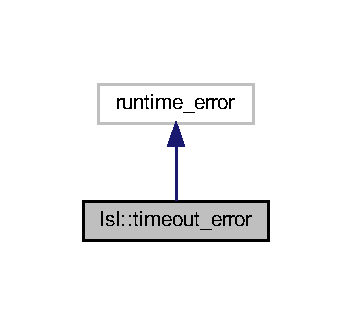
\includegraphics[width=169pt]{d9/d05/classlsl_1_1timeout__error__inherit__graph}
\end{center}
\end{figure}


Collaboration diagram for lsl\+:\+:timeout\+\_\+error\+:\nopagebreak
\begin{figure}[H]
\begin{center}
\leavevmode
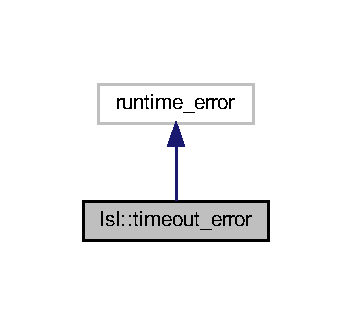
\includegraphics[width=169pt]{d4/d2c/classlsl_1_1timeout__error__coll__graph}
\end{center}
\end{figure}
\subsection*{Public Member Functions}
\begin{DoxyCompactItemize}
\item 
\hyperlink{classlsl_1_1timeout__error_afbc3b7c957fe3da4021aff3c30e6192f}{timeout\+\_\+error} (const std\+::string \&msg)
\end{DoxyCompactItemize}


\subsection{Detailed Description}
Exception class that indicates that an operation failed due to a timeout. 

\subsection{Constructor \& Destructor Documentation}
\mbox{\Hypertarget{classlsl_1_1timeout__error_afbc3b7c957fe3da4021aff3c30e6192f}\label{classlsl_1_1timeout__error_afbc3b7c957fe3da4021aff3c30e6192f}} 
\index{lsl\+::timeout\+\_\+error@{lsl\+::timeout\+\_\+error}!timeout\+\_\+error@{timeout\+\_\+error}}
\index{timeout\+\_\+error@{timeout\+\_\+error}!lsl\+::timeout\+\_\+error@{lsl\+::timeout\+\_\+error}}
\subsubsection{\texorpdfstring{timeout\+\_\+error()}{timeout\_error()}}
{\footnotesize\ttfamily lsl\+::timeout\+\_\+error\+::timeout\+\_\+error (\begin{DoxyParamCaption}\item[{const std\+::string \&}]{msg }\end{DoxyParamCaption})\hspace{0.3cm}{\ttfamily [inline]}, {\ttfamily [explicit]}}



The documentation for this class was generated from the following file\+:\begin{DoxyCompactItemize}
\item 
include/\hyperlink{lsl__cpp_8h}{lsl\+\_\+cpp.\+h}\end{DoxyCompactItemize}

\hypertarget{class_ui___main_window}{}\section{Ui\+\_\+\+Main\+Window Class Reference}
\label{class_ui___main_window}\index{Ui\+\_\+\+Main\+Window@{Ui\+\_\+\+Main\+Window}}


{\ttfamily \#include $<$ui\+\_\+mainwindow.\+h$>$}



Inheritance diagram for Ui\+\_\+\+Main\+Window\+:
\nopagebreak
\begin{figure}[H]
\begin{center}
\leavevmode
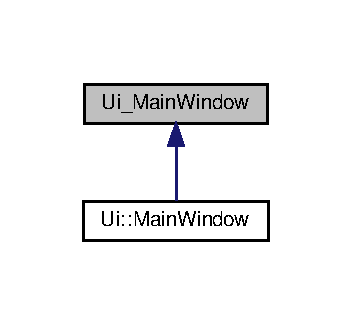
\includegraphics[width=169pt]{dd/df1/class_ui___main_window__inherit__graph}
\end{center}
\end{figure}
\subsection*{Public Member Functions}
\begin{DoxyCompactItemize}
\item 
void \hyperlink{class_ui___main_window_acf4a0872c4c77d8f43a2ec66ed849b58}{setup\+Ui} (Q\+Main\+Window $\ast$\hyperlink{class_main_window}{Main\+Window})
\item 
void \hyperlink{class_ui___main_window_a097dd160c3534a204904cb374412c618}{retranslate\+Ui} (Q\+Main\+Window $\ast$\hyperlink{class_main_window}{Main\+Window})
\end{DoxyCompactItemize}
\subsection*{Public Attributes}
\begin{DoxyCompactItemize}
\item 
Q\+Widget $\ast$ \hyperlink{class_ui___main_window_a30075506c2116c3ed4ff25e07ae75f81}{central\+Widget}
\item 
Q\+Grid\+Layout $\ast$ \hyperlink{class_ui___main_window_a525ed3c5fe0784ac502ee222fba4e205}{grid\+Layout}
\item 
Q\+Check\+Box $\ast$ \hyperlink{class_ui___main_window_a5a712f0294a7c1137b91e546a67d9cb7}{check\+Box\+\_\+\+R\+E\+C\+\_\+\+ON}
\item 
Q\+Tree\+Widget $\ast$ \hyperlink{class_ui___main_window_a082c92b8f4b52f2160ba8c58e94118c8}{tree\+Widget}
\item 
Q\+Label $\ast$ \hyperlink{class_ui___main_window_a663f728e6244926a795c6e6892673b1d}{label\+\_\+6}
\item 
Q\+Label $\ast$ \hyperlink{class_ui___main_window_ad9c89133780f28e6efa2ec17ceb9cff5}{label}
\item 
Q\+Frame $\ast$ \hyperlink{class_ui___main_window_a16e802a7ebd4beb9d8aba858565e51b3}{line}
\item 
Q\+Frame $\ast$ \hyperlink{class_ui___main_window_add492bf5763815e82fba9ba9297c50e6}{line\+\_\+4}
\item 
Q\+Check\+Box $\ast$ \hyperlink{class_ui___main_window_a6577339cac5354cd92212d8182b9b47d}{check\+Box\+\_\+\+D\+E\+C\+IM}
\item 
Q\+Label $\ast$ \hyperlink{class_ui___main_window_a78c7e10730b43c6700cd7216911ed76a}{label\+\_\+4}
\item 
Q\+Label $\ast$ \hyperlink{class_ui___main_window_ad6bab8fb8903b8f41afea1218ee52695}{label\+\_\+5}
\item 
Q\+Combo\+Box $\ast$ \hyperlink{class_ui___main_window_a60e6e7aea7048e8119b9cb05c2192070}{combo\+Box\+\_\+\+N\+CH}
\item 
Q\+Grid\+Layout $\ast$ \hyperlink{class_ui___main_window_a6b2a0c5f7e8ff2a87134908dd770d2d2}{grid\+Layout\+\_\+2}
\item 
Q\+Label $\ast$ \hyperlink{class_ui___main_window_af183bfbfb9f38bbdd60caf92b15e23dc}{label\+\_\+8}
\item 
Q\+Label $\ast$ \hyperlink{class_ui___main_window_a0e90c7e9ad77386881e0b264ddb9dd22}{label\+\_\+9}
\item 
Q\+Label $\ast$ \hyperlink{class_ui___main_window_a13936e6f18b1c90402b3c7a3c92b6cdb}{label\+\_\+7}
\item 
Q\+Combo\+Box $\ast$ \hyperlink{class_ui___main_window_ae8d1b45c0cfcd6b434a75a17c9037a1c}{combo\+Box\+\_\+\+I\+N\+S\+EL}
\item 
Q\+Combo\+Box $\ast$ \hyperlink{class_ui___main_window_a967a6487fae379c728b22caf95f5e83f}{combo\+Box\+\_\+\+C\+H\+S\+EL}
\item 
Q\+Combo\+Box $\ast$ \hyperlink{class_ui___main_window_a11ba7790a2147e039fd80cd3330a93f6}{combo\+Box\+\_\+\+A\+N\+O\+U\+T\+\_\+\+G\+A\+IN}
\item 
Q\+Grid\+Layout $\ast$ \hyperlink{class_ui___main_window_a8ee86315639f324b17708efc7dbe8b19}{grid\+Layout\+\_\+4}
\item 
Q\+Combo\+Box $\ast$ \hyperlink{class_ui___main_window_aaa3d8dbf2ffc2b6ea072f7ef88d1e5a0}{combo\+Box\+\_\+\+H\+PF}
\item 
Q\+Label $\ast$ \hyperlink{class_ui___main_window_a882200d8ae16962f5dd3b749ebacbf7e}{label\+\_\+15}
\item 
Q\+Label $\ast$ \hyperlink{class_ui___main_window_a9dc4dba26b83e0c94aa566e1c564420b}{label\+\_\+10}
\item 
Q\+Combo\+Box $\ast$ \hyperlink{class_ui___main_window_a25922bf1e0c13b9aac0498e48bdbbc2e}{combo\+Box\+\_\+selected\+IN}
\item 
Q\+Combo\+Box $\ast$ \hyperlink{class_ui___main_window_a16c04ddf40af3d97418246cfb04d9f82}{combo\+Box\+\_\+\+M\+O\+DE}
\item 
Q\+Combo\+Box $\ast$ \hyperlink{class_ui___main_window_a9e0aafa995e96d5c4dceba7788e29358}{combo\+Box\+\_\+\+L\+PF}
\item 
Q\+Frame $\ast$ \hyperlink{class_ui___main_window_a27e0b134c3c12643afbf0b50dd175453}{line\+\_\+3}
\item 
Q\+Combo\+Box $\ast$ \hyperlink{class_ui___main_window_a21522c20bae36c7f4ba4cb2354a8b17d}{combo\+Box\+\_\+\+A\+D\+A\+PT}
\item 
Q\+Combo\+Box $\ast$ \hyperlink{class_ui___main_window_aeb8291dc37be1a33337d1e403d07ed37}{combo\+Box\+\_\+\+S\+E\+NS}
\item 
Q\+Label $\ast$ \hyperlink{class_ui___main_window_a1c16c0a684617927472e534822a63c7d}{label\+\_\+14}
\item 
Q\+Label $\ast$ \hyperlink{class_ui___main_window_ab6ac4329a89041f557332f6569d94493}{label\+\_\+16}
\item 
Q\+Label $\ast$ \hyperlink{class_ui___main_window_a4f12a71b4a2fb6f85df2300d83b5ed3e}{label\+\_\+11}
\item 
Q\+Label $\ast$ \hyperlink{class_ui___main_window_ac1cbc41e9dbaeb3d0bdc2189d8e9ee1d}{label\+\_\+13}
\item 
Q\+Label $\ast$ \hyperlink{class_ui___main_window_aa2621565827195e88436fb54220bb48d}{label\+\_\+12}
\item 
Q\+Combo\+Box $\ast$ \hyperlink{class_ui___main_window_a35b1e7da83de7512c86d48f2d9f15b05}{combo\+Box\+\_\+\+S\+I\+DE}
\item 
Q\+Label $\ast$ \hyperlink{class_ui___main_window_a1f4ff90c122fededcc08604401442034}{label\+\_\+17}
\item 
Q\+Combo\+Box $\ast$ \hyperlink{class_ui___main_window_a6e4c09cd05089b1bd6081c4431be98e9}{combo\+Box\+\_\+\+M\+US}
\item 
Q\+Label $\ast$ \hyperlink{class_ui___main_window_a2e2516d755e4dd53fc905dabddf2738a}{label\+\_\+2}
\item 
Q\+Grid\+Layout $\ast$ \hyperlink{class_ui___main_window_a8731b71c513ff94baf59614807823c5d}{grid\+Layout\+\_\+5}
\item 
Q\+Push\+Button $\ast$ \hyperlink{class_ui___main_window_a257d4df0fe652a526e4fddba93c7a7d8}{push\+Button\+\_\+save}
\item 
Q\+Line\+Edit $\ast$ \hyperlink{class_ui___main_window_ad3416cfca3fcdab703d11bce1823e72e}{line\+Edit\+\_\+filepath}
\item 
Q\+Label $\ast$ \hyperlink{class_ui___main_window_a55100f53189f25cf8a1ee0beb29be642}{label\+\_\+18}
\item 
Q\+Push\+Button $\ast$ \hyperlink{class_ui___main_window_a3caafe0edcf60acd912b378ad151ceba}{push\+Button\+\_\+open}
\item 
Q\+Combo\+Box $\ast$ \hyperlink{class_ui___main_window_aaf7751422702d5df5584a71119ceabbb}{combo\+Box\+\_\+\+F\+S\+A\+MP}
\item 
Q\+Frame $\ast$ \hyperlink{class_ui___main_window_a17207206e55a605ecc14a3534b7e575f}{line\+\_\+2}
\item 
Q\+Label $\ast$ \hyperlink{class_ui___main_window_a0376fd90247280e7c7957cc70628708c}{label\+\_\+3}
\item 
Q\+Frame $\ast$ \hyperlink{class_ui___main_window_a7fd61d9f66189e10dcae1147f0a48e04}{line\+\_\+5}
\item 
Q\+Menu\+Bar $\ast$ \hyperlink{class_ui___main_window_a2be1c24ec9adfca18e1dcc951931457f}{menu\+Bar}
\item 
Q\+Tool\+Bar $\ast$ \hyperlink{class_ui___main_window_a5172877001c8c7b4e0f6de50421867d1}{main\+Tool\+Bar}
\item 
Q\+Status\+Bar $\ast$ \hyperlink{class_ui___main_window_a50fa481337604bcc8bf68de18ab16ecd}{status\+Bar}
\end{DoxyCompactItemize}


\subsection{Member Function Documentation}
\mbox{\Hypertarget{class_ui___main_window_a097dd160c3534a204904cb374412c618}\label{class_ui___main_window_a097dd160c3534a204904cb374412c618}} 
\index{Ui\+\_\+\+Main\+Window@{Ui\+\_\+\+Main\+Window}!retranslate\+Ui@{retranslate\+Ui}}
\index{retranslate\+Ui@{retranslate\+Ui}!Ui\+\_\+\+Main\+Window@{Ui\+\_\+\+Main\+Window}}
\subsubsection{\texorpdfstring{retranslate\+Ui()}{retranslateUi()}}
{\footnotesize\ttfamily void Ui\+\_\+\+Main\+Window\+::retranslate\+Ui (\begin{DoxyParamCaption}\item[{Q\+Main\+Window $\ast$}]{Main\+Window }\end{DoxyParamCaption})\hspace{0.3cm}{\ttfamily [inline]}}

\mbox{\Hypertarget{class_ui___main_window_acf4a0872c4c77d8f43a2ec66ed849b58}\label{class_ui___main_window_acf4a0872c4c77d8f43a2ec66ed849b58}} 
\index{Ui\+\_\+\+Main\+Window@{Ui\+\_\+\+Main\+Window}!setup\+Ui@{setup\+Ui}}
\index{setup\+Ui@{setup\+Ui}!Ui\+\_\+\+Main\+Window@{Ui\+\_\+\+Main\+Window}}
\subsubsection{\texorpdfstring{setup\+Ui()}{setupUi()}}
{\footnotesize\ttfamily void Ui\+\_\+\+Main\+Window\+::setup\+Ui (\begin{DoxyParamCaption}\item[{Q\+Main\+Window $\ast$}]{Main\+Window }\end{DoxyParamCaption})\hspace{0.3cm}{\ttfamily [inline]}}



\subsection{Member Data Documentation}
\mbox{\Hypertarget{class_ui___main_window_a30075506c2116c3ed4ff25e07ae75f81}\label{class_ui___main_window_a30075506c2116c3ed4ff25e07ae75f81}} 
\index{Ui\+\_\+\+Main\+Window@{Ui\+\_\+\+Main\+Window}!central\+Widget@{central\+Widget}}
\index{central\+Widget@{central\+Widget}!Ui\+\_\+\+Main\+Window@{Ui\+\_\+\+Main\+Window}}
\subsubsection{\texorpdfstring{central\+Widget}{centralWidget}}
{\footnotesize\ttfamily Q\+Widget$\ast$ Ui\+\_\+\+Main\+Window\+::central\+Widget}

\mbox{\Hypertarget{class_ui___main_window_a6577339cac5354cd92212d8182b9b47d}\label{class_ui___main_window_a6577339cac5354cd92212d8182b9b47d}} 
\index{Ui\+\_\+\+Main\+Window@{Ui\+\_\+\+Main\+Window}!check\+Box\+\_\+\+D\+E\+C\+IM@{check\+Box\+\_\+\+D\+E\+C\+IM}}
\index{check\+Box\+\_\+\+D\+E\+C\+IM@{check\+Box\+\_\+\+D\+E\+C\+IM}!Ui\+\_\+\+Main\+Window@{Ui\+\_\+\+Main\+Window}}
\subsubsection{\texorpdfstring{check\+Box\+\_\+\+D\+E\+C\+IM}{checkBox\_DECIM}}
{\footnotesize\ttfamily Q\+Check\+Box$\ast$ Ui\+\_\+\+Main\+Window\+::check\+Box\+\_\+\+D\+E\+C\+IM}

\mbox{\Hypertarget{class_ui___main_window_a5a712f0294a7c1137b91e546a67d9cb7}\label{class_ui___main_window_a5a712f0294a7c1137b91e546a67d9cb7}} 
\index{Ui\+\_\+\+Main\+Window@{Ui\+\_\+\+Main\+Window}!check\+Box\+\_\+\+R\+E\+C\+\_\+\+ON@{check\+Box\+\_\+\+R\+E\+C\+\_\+\+ON}}
\index{check\+Box\+\_\+\+R\+E\+C\+\_\+\+ON@{check\+Box\+\_\+\+R\+E\+C\+\_\+\+ON}!Ui\+\_\+\+Main\+Window@{Ui\+\_\+\+Main\+Window}}
\subsubsection{\texorpdfstring{check\+Box\+\_\+\+R\+E\+C\+\_\+\+ON}{checkBox\_REC\_ON}}
{\footnotesize\ttfamily Q\+Check\+Box$\ast$ Ui\+\_\+\+Main\+Window\+::check\+Box\+\_\+\+R\+E\+C\+\_\+\+ON}

\mbox{\Hypertarget{class_ui___main_window_a21522c20bae36c7f4ba4cb2354a8b17d}\label{class_ui___main_window_a21522c20bae36c7f4ba4cb2354a8b17d}} 
\index{Ui\+\_\+\+Main\+Window@{Ui\+\_\+\+Main\+Window}!combo\+Box\+\_\+\+A\+D\+A\+PT@{combo\+Box\+\_\+\+A\+D\+A\+PT}}
\index{combo\+Box\+\_\+\+A\+D\+A\+PT@{combo\+Box\+\_\+\+A\+D\+A\+PT}!Ui\+\_\+\+Main\+Window@{Ui\+\_\+\+Main\+Window}}
\subsubsection{\texorpdfstring{combo\+Box\+\_\+\+A\+D\+A\+PT}{comboBox\_ADAPT}}
{\footnotesize\ttfamily Q\+Combo\+Box$\ast$ Ui\+\_\+\+Main\+Window\+::combo\+Box\+\_\+\+A\+D\+A\+PT}

\mbox{\Hypertarget{class_ui___main_window_a11ba7790a2147e039fd80cd3330a93f6}\label{class_ui___main_window_a11ba7790a2147e039fd80cd3330a93f6}} 
\index{Ui\+\_\+\+Main\+Window@{Ui\+\_\+\+Main\+Window}!combo\+Box\+\_\+\+A\+N\+O\+U\+T\+\_\+\+G\+A\+IN@{combo\+Box\+\_\+\+A\+N\+O\+U\+T\+\_\+\+G\+A\+IN}}
\index{combo\+Box\+\_\+\+A\+N\+O\+U\+T\+\_\+\+G\+A\+IN@{combo\+Box\+\_\+\+A\+N\+O\+U\+T\+\_\+\+G\+A\+IN}!Ui\+\_\+\+Main\+Window@{Ui\+\_\+\+Main\+Window}}
\subsubsection{\texorpdfstring{combo\+Box\+\_\+\+A\+N\+O\+U\+T\+\_\+\+G\+A\+IN}{comboBox\_ANOUT\_GAIN}}
{\footnotesize\ttfamily Q\+Combo\+Box$\ast$ Ui\+\_\+\+Main\+Window\+::combo\+Box\+\_\+\+A\+N\+O\+U\+T\+\_\+\+G\+A\+IN}

\mbox{\Hypertarget{class_ui___main_window_a967a6487fae379c728b22caf95f5e83f}\label{class_ui___main_window_a967a6487fae379c728b22caf95f5e83f}} 
\index{Ui\+\_\+\+Main\+Window@{Ui\+\_\+\+Main\+Window}!combo\+Box\+\_\+\+C\+H\+S\+EL@{combo\+Box\+\_\+\+C\+H\+S\+EL}}
\index{combo\+Box\+\_\+\+C\+H\+S\+EL@{combo\+Box\+\_\+\+C\+H\+S\+EL}!Ui\+\_\+\+Main\+Window@{Ui\+\_\+\+Main\+Window}}
\subsubsection{\texorpdfstring{combo\+Box\+\_\+\+C\+H\+S\+EL}{comboBox\_CHSEL}}
{\footnotesize\ttfamily Q\+Combo\+Box$\ast$ Ui\+\_\+\+Main\+Window\+::combo\+Box\+\_\+\+C\+H\+S\+EL}

\mbox{\Hypertarget{class_ui___main_window_aaf7751422702d5df5584a71119ceabbb}\label{class_ui___main_window_aaf7751422702d5df5584a71119ceabbb}} 
\index{Ui\+\_\+\+Main\+Window@{Ui\+\_\+\+Main\+Window}!combo\+Box\+\_\+\+F\+S\+A\+MP@{combo\+Box\+\_\+\+F\+S\+A\+MP}}
\index{combo\+Box\+\_\+\+F\+S\+A\+MP@{combo\+Box\+\_\+\+F\+S\+A\+MP}!Ui\+\_\+\+Main\+Window@{Ui\+\_\+\+Main\+Window}}
\subsubsection{\texorpdfstring{combo\+Box\+\_\+\+F\+S\+A\+MP}{comboBox\_FSAMP}}
{\footnotesize\ttfamily Q\+Combo\+Box$\ast$ Ui\+\_\+\+Main\+Window\+::combo\+Box\+\_\+\+F\+S\+A\+MP}

\mbox{\Hypertarget{class_ui___main_window_aaa3d8dbf2ffc2b6ea072f7ef88d1e5a0}\label{class_ui___main_window_aaa3d8dbf2ffc2b6ea072f7ef88d1e5a0}} 
\index{Ui\+\_\+\+Main\+Window@{Ui\+\_\+\+Main\+Window}!combo\+Box\+\_\+\+H\+PF@{combo\+Box\+\_\+\+H\+PF}}
\index{combo\+Box\+\_\+\+H\+PF@{combo\+Box\+\_\+\+H\+PF}!Ui\+\_\+\+Main\+Window@{Ui\+\_\+\+Main\+Window}}
\subsubsection{\texorpdfstring{combo\+Box\+\_\+\+H\+PF}{comboBox\_HPF}}
{\footnotesize\ttfamily Q\+Combo\+Box$\ast$ Ui\+\_\+\+Main\+Window\+::combo\+Box\+\_\+\+H\+PF}

\mbox{\Hypertarget{class_ui___main_window_ae8d1b45c0cfcd6b434a75a17c9037a1c}\label{class_ui___main_window_ae8d1b45c0cfcd6b434a75a17c9037a1c}} 
\index{Ui\+\_\+\+Main\+Window@{Ui\+\_\+\+Main\+Window}!combo\+Box\+\_\+\+I\+N\+S\+EL@{combo\+Box\+\_\+\+I\+N\+S\+EL}}
\index{combo\+Box\+\_\+\+I\+N\+S\+EL@{combo\+Box\+\_\+\+I\+N\+S\+EL}!Ui\+\_\+\+Main\+Window@{Ui\+\_\+\+Main\+Window}}
\subsubsection{\texorpdfstring{combo\+Box\+\_\+\+I\+N\+S\+EL}{comboBox\_INSEL}}
{\footnotesize\ttfamily Q\+Combo\+Box$\ast$ Ui\+\_\+\+Main\+Window\+::combo\+Box\+\_\+\+I\+N\+S\+EL}

\mbox{\Hypertarget{class_ui___main_window_a9e0aafa995e96d5c4dceba7788e29358}\label{class_ui___main_window_a9e0aafa995e96d5c4dceba7788e29358}} 
\index{Ui\+\_\+\+Main\+Window@{Ui\+\_\+\+Main\+Window}!combo\+Box\+\_\+\+L\+PF@{combo\+Box\+\_\+\+L\+PF}}
\index{combo\+Box\+\_\+\+L\+PF@{combo\+Box\+\_\+\+L\+PF}!Ui\+\_\+\+Main\+Window@{Ui\+\_\+\+Main\+Window}}
\subsubsection{\texorpdfstring{combo\+Box\+\_\+\+L\+PF}{comboBox\_LPF}}
{\footnotesize\ttfamily Q\+Combo\+Box$\ast$ Ui\+\_\+\+Main\+Window\+::combo\+Box\+\_\+\+L\+PF}

\mbox{\Hypertarget{class_ui___main_window_a16c04ddf40af3d97418246cfb04d9f82}\label{class_ui___main_window_a16c04ddf40af3d97418246cfb04d9f82}} 
\index{Ui\+\_\+\+Main\+Window@{Ui\+\_\+\+Main\+Window}!combo\+Box\+\_\+\+M\+O\+DE@{combo\+Box\+\_\+\+M\+O\+DE}}
\index{combo\+Box\+\_\+\+M\+O\+DE@{combo\+Box\+\_\+\+M\+O\+DE}!Ui\+\_\+\+Main\+Window@{Ui\+\_\+\+Main\+Window}}
\subsubsection{\texorpdfstring{combo\+Box\+\_\+\+M\+O\+DE}{comboBox\_MODE}}
{\footnotesize\ttfamily Q\+Combo\+Box$\ast$ Ui\+\_\+\+Main\+Window\+::combo\+Box\+\_\+\+M\+O\+DE}

\mbox{\Hypertarget{class_ui___main_window_a6e4c09cd05089b1bd6081c4431be98e9}\label{class_ui___main_window_a6e4c09cd05089b1bd6081c4431be98e9}} 
\index{Ui\+\_\+\+Main\+Window@{Ui\+\_\+\+Main\+Window}!combo\+Box\+\_\+\+M\+US@{combo\+Box\+\_\+\+M\+US}}
\index{combo\+Box\+\_\+\+M\+US@{combo\+Box\+\_\+\+M\+US}!Ui\+\_\+\+Main\+Window@{Ui\+\_\+\+Main\+Window}}
\subsubsection{\texorpdfstring{combo\+Box\+\_\+\+M\+US}{comboBox\_MUS}}
{\footnotesize\ttfamily Q\+Combo\+Box$\ast$ Ui\+\_\+\+Main\+Window\+::combo\+Box\+\_\+\+M\+US}

\mbox{\Hypertarget{class_ui___main_window_a60e6e7aea7048e8119b9cb05c2192070}\label{class_ui___main_window_a60e6e7aea7048e8119b9cb05c2192070}} 
\index{Ui\+\_\+\+Main\+Window@{Ui\+\_\+\+Main\+Window}!combo\+Box\+\_\+\+N\+CH@{combo\+Box\+\_\+\+N\+CH}}
\index{combo\+Box\+\_\+\+N\+CH@{combo\+Box\+\_\+\+N\+CH}!Ui\+\_\+\+Main\+Window@{Ui\+\_\+\+Main\+Window}}
\subsubsection{\texorpdfstring{combo\+Box\+\_\+\+N\+CH}{comboBox\_NCH}}
{\footnotesize\ttfamily Q\+Combo\+Box$\ast$ Ui\+\_\+\+Main\+Window\+::combo\+Box\+\_\+\+N\+CH}

\mbox{\Hypertarget{class_ui___main_window_a25922bf1e0c13b9aac0498e48bdbbc2e}\label{class_ui___main_window_a25922bf1e0c13b9aac0498e48bdbbc2e}} 
\index{Ui\+\_\+\+Main\+Window@{Ui\+\_\+\+Main\+Window}!combo\+Box\+\_\+selected\+IN@{combo\+Box\+\_\+selected\+IN}}
\index{combo\+Box\+\_\+selected\+IN@{combo\+Box\+\_\+selected\+IN}!Ui\+\_\+\+Main\+Window@{Ui\+\_\+\+Main\+Window}}
\subsubsection{\texorpdfstring{combo\+Box\+\_\+selected\+IN}{comboBox\_selectedIN}}
{\footnotesize\ttfamily Q\+Combo\+Box$\ast$ Ui\+\_\+\+Main\+Window\+::combo\+Box\+\_\+selected\+IN}

\mbox{\Hypertarget{class_ui___main_window_aeb8291dc37be1a33337d1e403d07ed37}\label{class_ui___main_window_aeb8291dc37be1a33337d1e403d07ed37}} 
\index{Ui\+\_\+\+Main\+Window@{Ui\+\_\+\+Main\+Window}!combo\+Box\+\_\+\+S\+E\+NS@{combo\+Box\+\_\+\+S\+E\+NS}}
\index{combo\+Box\+\_\+\+S\+E\+NS@{combo\+Box\+\_\+\+S\+E\+NS}!Ui\+\_\+\+Main\+Window@{Ui\+\_\+\+Main\+Window}}
\subsubsection{\texorpdfstring{combo\+Box\+\_\+\+S\+E\+NS}{comboBox\_SENS}}
{\footnotesize\ttfamily Q\+Combo\+Box$\ast$ Ui\+\_\+\+Main\+Window\+::combo\+Box\+\_\+\+S\+E\+NS}

\mbox{\Hypertarget{class_ui___main_window_a35b1e7da83de7512c86d48f2d9f15b05}\label{class_ui___main_window_a35b1e7da83de7512c86d48f2d9f15b05}} 
\index{Ui\+\_\+\+Main\+Window@{Ui\+\_\+\+Main\+Window}!combo\+Box\+\_\+\+S\+I\+DE@{combo\+Box\+\_\+\+S\+I\+DE}}
\index{combo\+Box\+\_\+\+S\+I\+DE@{combo\+Box\+\_\+\+S\+I\+DE}!Ui\+\_\+\+Main\+Window@{Ui\+\_\+\+Main\+Window}}
\subsubsection{\texorpdfstring{combo\+Box\+\_\+\+S\+I\+DE}{comboBox\_SIDE}}
{\footnotesize\ttfamily Q\+Combo\+Box$\ast$ Ui\+\_\+\+Main\+Window\+::combo\+Box\+\_\+\+S\+I\+DE}

\mbox{\Hypertarget{class_ui___main_window_a525ed3c5fe0784ac502ee222fba4e205}\label{class_ui___main_window_a525ed3c5fe0784ac502ee222fba4e205}} 
\index{Ui\+\_\+\+Main\+Window@{Ui\+\_\+\+Main\+Window}!grid\+Layout@{grid\+Layout}}
\index{grid\+Layout@{grid\+Layout}!Ui\+\_\+\+Main\+Window@{Ui\+\_\+\+Main\+Window}}
\subsubsection{\texorpdfstring{grid\+Layout}{gridLayout}}
{\footnotesize\ttfamily Q\+Grid\+Layout$\ast$ Ui\+\_\+\+Main\+Window\+::grid\+Layout}

\mbox{\Hypertarget{class_ui___main_window_a6b2a0c5f7e8ff2a87134908dd770d2d2}\label{class_ui___main_window_a6b2a0c5f7e8ff2a87134908dd770d2d2}} 
\index{Ui\+\_\+\+Main\+Window@{Ui\+\_\+\+Main\+Window}!grid\+Layout\+\_\+2@{grid\+Layout\+\_\+2}}
\index{grid\+Layout\+\_\+2@{grid\+Layout\+\_\+2}!Ui\+\_\+\+Main\+Window@{Ui\+\_\+\+Main\+Window}}
\subsubsection{\texorpdfstring{grid\+Layout\+\_\+2}{gridLayout\_2}}
{\footnotesize\ttfamily Q\+Grid\+Layout$\ast$ Ui\+\_\+\+Main\+Window\+::grid\+Layout\+\_\+2}

\mbox{\Hypertarget{class_ui___main_window_a8ee86315639f324b17708efc7dbe8b19}\label{class_ui___main_window_a8ee86315639f324b17708efc7dbe8b19}} 
\index{Ui\+\_\+\+Main\+Window@{Ui\+\_\+\+Main\+Window}!grid\+Layout\+\_\+4@{grid\+Layout\+\_\+4}}
\index{grid\+Layout\+\_\+4@{grid\+Layout\+\_\+4}!Ui\+\_\+\+Main\+Window@{Ui\+\_\+\+Main\+Window}}
\subsubsection{\texorpdfstring{grid\+Layout\+\_\+4}{gridLayout\_4}}
{\footnotesize\ttfamily Q\+Grid\+Layout$\ast$ Ui\+\_\+\+Main\+Window\+::grid\+Layout\+\_\+4}

\mbox{\Hypertarget{class_ui___main_window_a8731b71c513ff94baf59614807823c5d}\label{class_ui___main_window_a8731b71c513ff94baf59614807823c5d}} 
\index{Ui\+\_\+\+Main\+Window@{Ui\+\_\+\+Main\+Window}!grid\+Layout\+\_\+5@{grid\+Layout\+\_\+5}}
\index{grid\+Layout\+\_\+5@{grid\+Layout\+\_\+5}!Ui\+\_\+\+Main\+Window@{Ui\+\_\+\+Main\+Window}}
\subsubsection{\texorpdfstring{grid\+Layout\+\_\+5}{gridLayout\_5}}
{\footnotesize\ttfamily Q\+Grid\+Layout$\ast$ Ui\+\_\+\+Main\+Window\+::grid\+Layout\+\_\+5}

\mbox{\Hypertarget{class_ui___main_window_ad9c89133780f28e6efa2ec17ceb9cff5}\label{class_ui___main_window_ad9c89133780f28e6efa2ec17ceb9cff5}} 
\index{Ui\+\_\+\+Main\+Window@{Ui\+\_\+\+Main\+Window}!label@{label}}
\index{label@{label}!Ui\+\_\+\+Main\+Window@{Ui\+\_\+\+Main\+Window}}
\subsubsection{\texorpdfstring{label}{label}}
{\footnotesize\ttfamily Q\+Label$\ast$ Ui\+\_\+\+Main\+Window\+::label}

\mbox{\Hypertarget{class_ui___main_window_a9dc4dba26b83e0c94aa566e1c564420b}\label{class_ui___main_window_a9dc4dba26b83e0c94aa566e1c564420b}} 
\index{Ui\+\_\+\+Main\+Window@{Ui\+\_\+\+Main\+Window}!label\+\_\+10@{label\+\_\+10}}
\index{label\+\_\+10@{label\+\_\+10}!Ui\+\_\+\+Main\+Window@{Ui\+\_\+\+Main\+Window}}
\subsubsection{\texorpdfstring{label\+\_\+10}{label\_10}}
{\footnotesize\ttfamily Q\+Label$\ast$ Ui\+\_\+\+Main\+Window\+::label\+\_\+10}

\mbox{\Hypertarget{class_ui___main_window_a4f12a71b4a2fb6f85df2300d83b5ed3e}\label{class_ui___main_window_a4f12a71b4a2fb6f85df2300d83b5ed3e}} 
\index{Ui\+\_\+\+Main\+Window@{Ui\+\_\+\+Main\+Window}!label\+\_\+11@{label\+\_\+11}}
\index{label\+\_\+11@{label\+\_\+11}!Ui\+\_\+\+Main\+Window@{Ui\+\_\+\+Main\+Window}}
\subsubsection{\texorpdfstring{label\+\_\+11}{label\_11}}
{\footnotesize\ttfamily Q\+Label$\ast$ Ui\+\_\+\+Main\+Window\+::label\+\_\+11}

\mbox{\Hypertarget{class_ui___main_window_aa2621565827195e88436fb54220bb48d}\label{class_ui___main_window_aa2621565827195e88436fb54220bb48d}} 
\index{Ui\+\_\+\+Main\+Window@{Ui\+\_\+\+Main\+Window}!label\+\_\+12@{label\+\_\+12}}
\index{label\+\_\+12@{label\+\_\+12}!Ui\+\_\+\+Main\+Window@{Ui\+\_\+\+Main\+Window}}
\subsubsection{\texorpdfstring{label\+\_\+12}{label\_12}}
{\footnotesize\ttfamily Q\+Label$\ast$ Ui\+\_\+\+Main\+Window\+::label\+\_\+12}

\mbox{\Hypertarget{class_ui___main_window_ac1cbc41e9dbaeb3d0bdc2189d8e9ee1d}\label{class_ui___main_window_ac1cbc41e9dbaeb3d0bdc2189d8e9ee1d}} 
\index{Ui\+\_\+\+Main\+Window@{Ui\+\_\+\+Main\+Window}!label\+\_\+13@{label\+\_\+13}}
\index{label\+\_\+13@{label\+\_\+13}!Ui\+\_\+\+Main\+Window@{Ui\+\_\+\+Main\+Window}}
\subsubsection{\texorpdfstring{label\+\_\+13}{label\_13}}
{\footnotesize\ttfamily Q\+Label$\ast$ Ui\+\_\+\+Main\+Window\+::label\+\_\+13}

\mbox{\Hypertarget{class_ui___main_window_a1c16c0a684617927472e534822a63c7d}\label{class_ui___main_window_a1c16c0a684617927472e534822a63c7d}} 
\index{Ui\+\_\+\+Main\+Window@{Ui\+\_\+\+Main\+Window}!label\+\_\+14@{label\+\_\+14}}
\index{label\+\_\+14@{label\+\_\+14}!Ui\+\_\+\+Main\+Window@{Ui\+\_\+\+Main\+Window}}
\subsubsection{\texorpdfstring{label\+\_\+14}{label\_14}}
{\footnotesize\ttfamily Q\+Label$\ast$ Ui\+\_\+\+Main\+Window\+::label\+\_\+14}

\mbox{\Hypertarget{class_ui___main_window_a882200d8ae16962f5dd3b749ebacbf7e}\label{class_ui___main_window_a882200d8ae16962f5dd3b749ebacbf7e}} 
\index{Ui\+\_\+\+Main\+Window@{Ui\+\_\+\+Main\+Window}!label\+\_\+15@{label\+\_\+15}}
\index{label\+\_\+15@{label\+\_\+15}!Ui\+\_\+\+Main\+Window@{Ui\+\_\+\+Main\+Window}}
\subsubsection{\texorpdfstring{label\+\_\+15}{label\_15}}
{\footnotesize\ttfamily Q\+Label$\ast$ Ui\+\_\+\+Main\+Window\+::label\+\_\+15}

\mbox{\Hypertarget{class_ui___main_window_ab6ac4329a89041f557332f6569d94493}\label{class_ui___main_window_ab6ac4329a89041f557332f6569d94493}} 
\index{Ui\+\_\+\+Main\+Window@{Ui\+\_\+\+Main\+Window}!label\+\_\+16@{label\+\_\+16}}
\index{label\+\_\+16@{label\+\_\+16}!Ui\+\_\+\+Main\+Window@{Ui\+\_\+\+Main\+Window}}
\subsubsection{\texorpdfstring{label\+\_\+16}{label\_16}}
{\footnotesize\ttfamily Q\+Label$\ast$ Ui\+\_\+\+Main\+Window\+::label\+\_\+16}

\mbox{\Hypertarget{class_ui___main_window_a1f4ff90c122fededcc08604401442034}\label{class_ui___main_window_a1f4ff90c122fededcc08604401442034}} 
\index{Ui\+\_\+\+Main\+Window@{Ui\+\_\+\+Main\+Window}!label\+\_\+17@{label\+\_\+17}}
\index{label\+\_\+17@{label\+\_\+17}!Ui\+\_\+\+Main\+Window@{Ui\+\_\+\+Main\+Window}}
\subsubsection{\texorpdfstring{label\+\_\+17}{label\_17}}
{\footnotesize\ttfamily Q\+Label$\ast$ Ui\+\_\+\+Main\+Window\+::label\+\_\+17}

\mbox{\Hypertarget{class_ui___main_window_a55100f53189f25cf8a1ee0beb29be642}\label{class_ui___main_window_a55100f53189f25cf8a1ee0beb29be642}} 
\index{Ui\+\_\+\+Main\+Window@{Ui\+\_\+\+Main\+Window}!label\+\_\+18@{label\+\_\+18}}
\index{label\+\_\+18@{label\+\_\+18}!Ui\+\_\+\+Main\+Window@{Ui\+\_\+\+Main\+Window}}
\subsubsection{\texorpdfstring{label\+\_\+18}{label\_18}}
{\footnotesize\ttfamily Q\+Label$\ast$ Ui\+\_\+\+Main\+Window\+::label\+\_\+18}

\mbox{\Hypertarget{class_ui___main_window_a2e2516d755e4dd53fc905dabddf2738a}\label{class_ui___main_window_a2e2516d755e4dd53fc905dabddf2738a}} 
\index{Ui\+\_\+\+Main\+Window@{Ui\+\_\+\+Main\+Window}!label\+\_\+2@{label\+\_\+2}}
\index{label\+\_\+2@{label\+\_\+2}!Ui\+\_\+\+Main\+Window@{Ui\+\_\+\+Main\+Window}}
\subsubsection{\texorpdfstring{label\+\_\+2}{label\_2}}
{\footnotesize\ttfamily Q\+Label$\ast$ Ui\+\_\+\+Main\+Window\+::label\+\_\+2}

\mbox{\Hypertarget{class_ui___main_window_a0376fd90247280e7c7957cc70628708c}\label{class_ui___main_window_a0376fd90247280e7c7957cc70628708c}} 
\index{Ui\+\_\+\+Main\+Window@{Ui\+\_\+\+Main\+Window}!label\+\_\+3@{label\+\_\+3}}
\index{label\+\_\+3@{label\+\_\+3}!Ui\+\_\+\+Main\+Window@{Ui\+\_\+\+Main\+Window}}
\subsubsection{\texorpdfstring{label\+\_\+3}{label\_3}}
{\footnotesize\ttfamily Q\+Label$\ast$ Ui\+\_\+\+Main\+Window\+::label\+\_\+3}

\mbox{\Hypertarget{class_ui___main_window_a78c7e10730b43c6700cd7216911ed76a}\label{class_ui___main_window_a78c7e10730b43c6700cd7216911ed76a}} 
\index{Ui\+\_\+\+Main\+Window@{Ui\+\_\+\+Main\+Window}!label\+\_\+4@{label\+\_\+4}}
\index{label\+\_\+4@{label\+\_\+4}!Ui\+\_\+\+Main\+Window@{Ui\+\_\+\+Main\+Window}}
\subsubsection{\texorpdfstring{label\+\_\+4}{label\_4}}
{\footnotesize\ttfamily Q\+Label$\ast$ Ui\+\_\+\+Main\+Window\+::label\+\_\+4}

\mbox{\Hypertarget{class_ui___main_window_ad6bab8fb8903b8f41afea1218ee52695}\label{class_ui___main_window_ad6bab8fb8903b8f41afea1218ee52695}} 
\index{Ui\+\_\+\+Main\+Window@{Ui\+\_\+\+Main\+Window}!label\+\_\+5@{label\+\_\+5}}
\index{label\+\_\+5@{label\+\_\+5}!Ui\+\_\+\+Main\+Window@{Ui\+\_\+\+Main\+Window}}
\subsubsection{\texorpdfstring{label\+\_\+5}{label\_5}}
{\footnotesize\ttfamily Q\+Label$\ast$ Ui\+\_\+\+Main\+Window\+::label\+\_\+5}

\mbox{\Hypertarget{class_ui___main_window_a663f728e6244926a795c6e6892673b1d}\label{class_ui___main_window_a663f728e6244926a795c6e6892673b1d}} 
\index{Ui\+\_\+\+Main\+Window@{Ui\+\_\+\+Main\+Window}!label\+\_\+6@{label\+\_\+6}}
\index{label\+\_\+6@{label\+\_\+6}!Ui\+\_\+\+Main\+Window@{Ui\+\_\+\+Main\+Window}}
\subsubsection{\texorpdfstring{label\+\_\+6}{label\_6}}
{\footnotesize\ttfamily Q\+Label$\ast$ Ui\+\_\+\+Main\+Window\+::label\+\_\+6}

\mbox{\Hypertarget{class_ui___main_window_a13936e6f18b1c90402b3c7a3c92b6cdb}\label{class_ui___main_window_a13936e6f18b1c90402b3c7a3c92b6cdb}} 
\index{Ui\+\_\+\+Main\+Window@{Ui\+\_\+\+Main\+Window}!label\+\_\+7@{label\+\_\+7}}
\index{label\+\_\+7@{label\+\_\+7}!Ui\+\_\+\+Main\+Window@{Ui\+\_\+\+Main\+Window}}
\subsubsection{\texorpdfstring{label\+\_\+7}{label\_7}}
{\footnotesize\ttfamily Q\+Label$\ast$ Ui\+\_\+\+Main\+Window\+::label\+\_\+7}

\mbox{\Hypertarget{class_ui___main_window_af183bfbfb9f38bbdd60caf92b15e23dc}\label{class_ui___main_window_af183bfbfb9f38bbdd60caf92b15e23dc}} 
\index{Ui\+\_\+\+Main\+Window@{Ui\+\_\+\+Main\+Window}!label\+\_\+8@{label\+\_\+8}}
\index{label\+\_\+8@{label\+\_\+8}!Ui\+\_\+\+Main\+Window@{Ui\+\_\+\+Main\+Window}}
\subsubsection{\texorpdfstring{label\+\_\+8}{label\_8}}
{\footnotesize\ttfamily Q\+Label$\ast$ Ui\+\_\+\+Main\+Window\+::label\+\_\+8}

\mbox{\Hypertarget{class_ui___main_window_a0e90c7e9ad77386881e0b264ddb9dd22}\label{class_ui___main_window_a0e90c7e9ad77386881e0b264ddb9dd22}} 
\index{Ui\+\_\+\+Main\+Window@{Ui\+\_\+\+Main\+Window}!label\+\_\+9@{label\+\_\+9}}
\index{label\+\_\+9@{label\+\_\+9}!Ui\+\_\+\+Main\+Window@{Ui\+\_\+\+Main\+Window}}
\subsubsection{\texorpdfstring{label\+\_\+9}{label\_9}}
{\footnotesize\ttfamily Q\+Label$\ast$ Ui\+\_\+\+Main\+Window\+::label\+\_\+9}

\mbox{\Hypertarget{class_ui___main_window_a16e802a7ebd4beb9d8aba858565e51b3}\label{class_ui___main_window_a16e802a7ebd4beb9d8aba858565e51b3}} 
\index{Ui\+\_\+\+Main\+Window@{Ui\+\_\+\+Main\+Window}!line@{line}}
\index{line@{line}!Ui\+\_\+\+Main\+Window@{Ui\+\_\+\+Main\+Window}}
\subsubsection{\texorpdfstring{line}{line}}
{\footnotesize\ttfamily Q\+Frame$\ast$ Ui\+\_\+\+Main\+Window\+::line}

\mbox{\Hypertarget{class_ui___main_window_a17207206e55a605ecc14a3534b7e575f}\label{class_ui___main_window_a17207206e55a605ecc14a3534b7e575f}} 
\index{Ui\+\_\+\+Main\+Window@{Ui\+\_\+\+Main\+Window}!line\+\_\+2@{line\+\_\+2}}
\index{line\+\_\+2@{line\+\_\+2}!Ui\+\_\+\+Main\+Window@{Ui\+\_\+\+Main\+Window}}
\subsubsection{\texorpdfstring{line\+\_\+2}{line\_2}}
{\footnotesize\ttfamily Q\+Frame$\ast$ Ui\+\_\+\+Main\+Window\+::line\+\_\+2}

\mbox{\Hypertarget{class_ui___main_window_a27e0b134c3c12643afbf0b50dd175453}\label{class_ui___main_window_a27e0b134c3c12643afbf0b50dd175453}} 
\index{Ui\+\_\+\+Main\+Window@{Ui\+\_\+\+Main\+Window}!line\+\_\+3@{line\+\_\+3}}
\index{line\+\_\+3@{line\+\_\+3}!Ui\+\_\+\+Main\+Window@{Ui\+\_\+\+Main\+Window}}
\subsubsection{\texorpdfstring{line\+\_\+3}{line\_3}}
{\footnotesize\ttfamily Q\+Frame$\ast$ Ui\+\_\+\+Main\+Window\+::line\+\_\+3}

\mbox{\Hypertarget{class_ui___main_window_add492bf5763815e82fba9ba9297c50e6}\label{class_ui___main_window_add492bf5763815e82fba9ba9297c50e6}} 
\index{Ui\+\_\+\+Main\+Window@{Ui\+\_\+\+Main\+Window}!line\+\_\+4@{line\+\_\+4}}
\index{line\+\_\+4@{line\+\_\+4}!Ui\+\_\+\+Main\+Window@{Ui\+\_\+\+Main\+Window}}
\subsubsection{\texorpdfstring{line\+\_\+4}{line\_4}}
{\footnotesize\ttfamily Q\+Frame$\ast$ Ui\+\_\+\+Main\+Window\+::line\+\_\+4}

\mbox{\Hypertarget{class_ui___main_window_a7fd61d9f66189e10dcae1147f0a48e04}\label{class_ui___main_window_a7fd61d9f66189e10dcae1147f0a48e04}} 
\index{Ui\+\_\+\+Main\+Window@{Ui\+\_\+\+Main\+Window}!line\+\_\+5@{line\+\_\+5}}
\index{line\+\_\+5@{line\+\_\+5}!Ui\+\_\+\+Main\+Window@{Ui\+\_\+\+Main\+Window}}
\subsubsection{\texorpdfstring{line\+\_\+5}{line\_5}}
{\footnotesize\ttfamily Q\+Frame$\ast$ Ui\+\_\+\+Main\+Window\+::line\+\_\+5}

\mbox{\Hypertarget{class_ui___main_window_ad3416cfca3fcdab703d11bce1823e72e}\label{class_ui___main_window_ad3416cfca3fcdab703d11bce1823e72e}} 
\index{Ui\+\_\+\+Main\+Window@{Ui\+\_\+\+Main\+Window}!line\+Edit\+\_\+filepath@{line\+Edit\+\_\+filepath}}
\index{line\+Edit\+\_\+filepath@{line\+Edit\+\_\+filepath}!Ui\+\_\+\+Main\+Window@{Ui\+\_\+\+Main\+Window}}
\subsubsection{\texorpdfstring{line\+Edit\+\_\+filepath}{lineEdit\_filepath}}
{\footnotesize\ttfamily Q\+Line\+Edit$\ast$ Ui\+\_\+\+Main\+Window\+::line\+Edit\+\_\+filepath}

\mbox{\Hypertarget{class_ui___main_window_a5172877001c8c7b4e0f6de50421867d1}\label{class_ui___main_window_a5172877001c8c7b4e0f6de50421867d1}} 
\index{Ui\+\_\+\+Main\+Window@{Ui\+\_\+\+Main\+Window}!main\+Tool\+Bar@{main\+Tool\+Bar}}
\index{main\+Tool\+Bar@{main\+Tool\+Bar}!Ui\+\_\+\+Main\+Window@{Ui\+\_\+\+Main\+Window}}
\subsubsection{\texorpdfstring{main\+Tool\+Bar}{mainToolBar}}
{\footnotesize\ttfamily Q\+Tool\+Bar$\ast$ Ui\+\_\+\+Main\+Window\+::main\+Tool\+Bar}

\mbox{\Hypertarget{class_ui___main_window_a2be1c24ec9adfca18e1dcc951931457f}\label{class_ui___main_window_a2be1c24ec9adfca18e1dcc951931457f}} 
\index{Ui\+\_\+\+Main\+Window@{Ui\+\_\+\+Main\+Window}!menu\+Bar@{menu\+Bar}}
\index{menu\+Bar@{menu\+Bar}!Ui\+\_\+\+Main\+Window@{Ui\+\_\+\+Main\+Window}}
\subsubsection{\texorpdfstring{menu\+Bar}{menuBar}}
{\footnotesize\ttfamily Q\+Menu\+Bar$\ast$ Ui\+\_\+\+Main\+Window\+::menu\+Bar}

\mbox{\Hypertarget{class_ui___main_window_a3caafe0edcf60acd912b378ad151ceba}\label{class_ui___main_window_a3caafe0edcf60acd912b378ad151ceba}} 
\index{Ui\+\_\+\+Main\+Window@{Ui\+\_\+\+Main\+Window}!push\+Button\+\_\+open@{push\+Button\+\_\+open}}
\index{push\+Button\+\_\+open@{push\+Button\+\_\+open}!Ui\+\_\+\+Main\+Window@{Ui\+\_\+\+Main\+Window}}
\subsubsection{\texorpdfstring{push\+Button\+\_\+open}{pushButton\_open}}
{\footnotesize\ttfamily Q\+Push\+Button$\ast$ Ui\+\_\+\+Main\+Window\+::push\+Button\+\_\+open}

\mbox{\Hypertarget{class_ui___main_window_a257d4df0fe652a526e4fddba93c7a7d8}\label{class_ui___main_window_a257d4df0fe652a526e4fddba93c7a7d8}} 
\index{Ui\+\_\+\+Main\+Window@{Ui\+\_\+\+Main\+Window}!push\+Button\+\_\+save@{push\+Button\+\_\+save}}
\index{push\+Button\+\_\+save@{push\+Button\+\_\+save}!Ui\+\_\+\+Main\+Window@{Ui\+\_\+\+Main\+Window}}
\subsubsection{\texorpdfstring{push\+Button\+\_\+save}{pushButton\_save}}
{\footnotesize\ttfamily Q\+Push\+Button$\ast$ Ui\+\_\+\+Main\+Window\+::push\+Button\+\_\+save}

\mbox{\Hypertarget{class_ui___main_window_a50fa481337604bcc8bf68de18ab16ecd}\label{class_ui___main_window_a50fa481337604bcc8bf68de18ab16ecd}} 
\index{Ui\+\_\+\+Main\+Window@{Ui\+\_\+\+Main\+Window}!status\+Bar@{status\+Bar}}
\index{status\+Bar@{status\+Bar}!Ui\+\_\+\+Main\+Window@{Ui\+\_\+\+Main\+Window}}
\subsubsection{\texorpdfstring{status\+Bar}{statusBar}}
{\footnotesize\ttfamily Q\+Status\+Bar$\ast$ Ui\+\_\+\+Main\+Window\+::status\+Bar}

\mbox{\Hypertarget{class_ui___main_window_a082c92b8f4b52f2160ba8c58e94118c8}\label{class_ui___main_window_a082c92b8f4b52f2160ba8c58e94118c8}} 
\index{Ui\+\_\+\+Main\+Window@{Ui\+\_\+\+Main\+Window}!tree\+Widget@{tree\+Widget}}
\index{tree\+Widget@{tree\+Widget}!Ui\+\_\+\+Main\+Window@{Ui\+\_\+\+Main\+Window}}
\subsubsection{\texorpdfstring{tree\+Widget}{treeWidget}}
{\footnotesize\ttfamily Q\+Tree\+Widget$\ast$ Ui\+\_\+\+Main\+Window\+::tree\+Widget}



The documentation for this class was generated from the following file\+:\begin{DoxyCompactItemize}
\item 
O\+T\+Bconfig\+G\+U\+I/build/\hyperlink{ui__mainwindow_8h}{ui\+\_\+mainwindow.\+h}\end{DoxyCompactItemize}

\hypertarget{classlsl_1_1xml__element}{}\section{lsl\+:\+:xml\+\_\+element Class Reference}
\label{classlsl_1_1xml__element}\index{lsl\+::xml\+\_\+element@{lsl\+::xml\+\_\+element}}


{\ttfamily \#include $<$lsl\+\_\+cpp.\+h$>$}

\subsection*{Public Member Functions}
\begin{DoxyCompactItemize}
\item 
\mbox{\Hypertarget{classlsl_1_1xml__element_a9a2c940a06714662f3cef5e9847e8cae}\label{classlsl_1_1xml__element_a9a2c940a06714662f3cef5e9847e8cae}} 
\hyperlink{classlsl_1_1xml__element_a9a2c940a06714662f3cef5e9847e8cae}{xml\+\_\+element} (\hyperlink{namespacelsl_a5edc7a49a1a1be1634fe6dce3d59c59b}{lsl\+\_\+xml\+\_\+ptr} obj=0)
\begin{DoxyCompactList}\small\item\em Constructor. \end{DoxyCompactList}\item 
\mbox{\Hypertarget{classlsl_1_1xml__element_ab68b7a1c63c2cb0eb4ce6361b94469b7}\label{classlsl_1_1xml__element_ab68b7a1c63c2cb0eb4ce6361b94469b7}} 
\hyperlink{classlsl_1_1xml__element}{xml\+\_\+element} \hyperlink{classlsl_1_1xml__element_ab68b7a1c63c2cb0eb4ce6361b94469b7}{first\+\_\+child} () const
\begin{DoxyCompactList}\small\item\em Get the first child of the element. \end{DoxyCompactList}\item 
\mbox{\Hypertarget{classlsl_1_1xml__element_a12254f735a79a11b75718fe7c28186d0}\label{classlsl_1_1xml__element_a12254f735a79a11b75718fe7c28186d0}} 
\hyperlink{classlsl_1_1xml__element}{xml\+\_\+element} \hyperlink{classlsl_1_1xml__element_a12254f735a79a11b75718fe7c28186d0}{last\+\_\+child} () const
\begin{DoxyCompactList}\small\item\em Get the last child of the element. \end{DoxyCompactList}\item 
\mbox{\Hypertarget{classlsl_1_1xml__element_a9637215f616b660789696e452b0e0591}\label{classlsl_1_1xml__element_a9637215f616b660789696e452b0e0591}} 
\hyperlink{classlsl_1_1xml__element}{xml\+\_\+element} \hyperlink{classlsl_1_1xml__element_a9637215f616b660789696e452b0e0591}{next\+\_\+sibling} () const
\begin{DoxyCompactList}\small\item\em Get the next sibling in the children list of the parent node. \end{DoxyCompactList}\item 
\mbox{\Hypertarget{classlsl_1_1xml__element_a78c2e0b3d7bda2b5a2d478e3c0cdc87a}\label{classlsl_1_1xml__element_a78c2e0b3d7bda2b5a2d478e3c0cdc87a}} 
\hyperlink{classlsl_1_1xml__element}{xml\+\_\+element} \hyperlink{classlsl_1_1xml__element_a78c2e0b3d7bda2b5a2d478e3c0cdc87a}{previous\+\_\+sibling} () const
\begin{DoxyCompactList}\small\item\em Get the previous sibling in the children list of the parent node. \end{DoxyCompactList}\item 
\mbox{\Hypertarget{classlsl_1_1xml__element_ae3211be3c10164f366220b638a9dd200}\label{classlsl_1_1xml__element_ae3211be3c10164f366220b638a9dd200}} 
\hyperlink{classlsl_1_1xml__element}{xml\+\_\+element} \hyperlink{classlsl_1_1xml__element_ae3211be3c10164f366220b638a9dd200}{parent} () const
\begin{DoxyCompactList}\small\item\em Get the parent node. \end{DoxyCompactList}\item 
\mbox{\Hypertarget{classlsl_1_1xml__element_a111ef129dce406af43948d8c9b915148}\label{classlsl_1_1xml__element_a111ef129dce406af43948d8c9b915148}} 
\hyperlink{classlsl_1_1xml__element}{xml\+\_\+element} \hyperlink{classlsl_1_1xml__element_a111ef129dce406af43948d8c9b915148}{child} (const std\+::string \&\hyperlink{classlsl_1_1xml__element_a2e449e85b7e763b1d0db4bb19d2eb7c2}{name}) const
\begin{DoxyCompactList}\small\item\em Get a child with a specified name. \end{DoxyCompactList}\item 
\mbox{\Hypertarget{classlsl_1_1xml__element_a100590d2a9822261a3f0b0ed7810134d}\label{classlsl_1_1xml__element_a100590d2a9822261a3f0b0ed7810134d}} 
\hyperlink{classlsl_1_1xml__element}{xml\+\_\+element} \hyperlink{classlsl_1_1xml__element_a100590d2a9822261a3f0b0ed7810134d}{next\+\_\+sibling} (const std\+::string \&\hyperlink{classlsl_1_1xml__element_a2e449e85b7e763b1d0db4bb19d2eb7c2}{name}) const
\begin{DoxyCompactList}\small\item\em Get the next sibling with the specified name. \end{DoxyCompactList}\item 
\mbox{\Hypertarget{classlsl_1_1xml__element_a70b90853b7edfaebfe69bc1103ed6b8b}\label{classlsl_1_1xml__element_a70b90853b7edfaebfe69bc1103ed6b8b}} 
\hyperlink{classlsl_1_1xml__element}{xml\+\_\+element} \hyperlink{classlsl_1_1xml__element_a70b90853b7edfaebfe69bc1103ed6b8b}{previous\+\_\+sibling} (const std\+::string \&\hyperlink{classlsl_1_1xml__element_a2e449e85b7e763b1d0db4bb19d2eb7c2}{name}) const
\begin{DoxyCompactList}\small\item\em Get the previous sibling with the specified name. \end{DoxyCompactList}\item 
\mbox{\Hypertarget{classlsl_1_1xml__element_a787dcaf85abcc5cd4d5f93fc80c82eb5}\label{classlsl_1_1xml__element_a787dcaf85abcc5cd4d5f93fc80c82eb5}} 
bool \hyperlink{classlsl_1_1xml__element_a787dcaf85abcc5cd4d5f93fc80c82eb5}{empty} () const
\begin{DoxyCompactList}\small\item\em Whether this node is empty. \end{DoxyCompactList}\item 
\mbox{\Hypertarget{classlsl_1_1xml__element_a965cfff9a29ebe6d8274f5256ff0017c}\label{classlsl_1_1xml__element_a965cfff9a29ebe6d8274f5256ff0017c}} 
bool \hyperlink{classlsl_1_1xml__element_a965cfff9a29ebe6d8274f5256ff0017c}{is\+\_\+text} () const
\begin{DoxyCompactList}\small\item\em Whether this is a text body (instead of an X\+ML element). True both for plain char data and C\+Data. \end{DoxyCompactList}\item 
\mbox{\Hypertarget{classlsl_1_1xml__element_a2e449e85b7e763b1d0db4bb19d2eb7c2}\label{classlsl_1_1xml__element_a2e449e85b7e763b1d0db4bb19d2eb7c2}} 
const char $\ast$ \hyperlink{classlsl_1_1xml__element_a2e449e85b7e763b1d0db4bb19d2eb7c2}{name} () const
\begin{DoxyCompactList}\small\item\em Name of the element. \end{DoxyCompactList}\item 
\mbox{\Hypertarget{classlsl_1_1xml__element_a1a5e666b35c5d7262e4ffbda86b57f73}\label{classlsl_1_1xml__element_a1a5e666b35c5d7262e4ffbda86b57f73}} 
const char $\ast$ \hyperlink{classlsl_1_1xml__element_a1a5e666b35c5d7262e4ffbda86b57f73}{value} () const
\begin{DoxyCompactList}\small\item\em Value of the element. \end{DoxyCompactList}\item 
\mbox{\Hypertarget{classlsl_1_1xml__element_ac99677d44f66ba850afd9b669e26452f}\label{classlsl_1_1xml__element_ac99677d44f66ba850afd9b669e26452f}} 
const char $\ast$ \hyperlink{classlsl_1_1xml__element_ac99677d44f66ba850afd9b669e26452f}{child\+\_\+value} () const
\begin{DoxyCompactList}\small\item\em Get child value (value of the first child that is text). \end{DoxyCompactList}\item 
\mbox{\Hypertarget{classlsl_1_1xml__element_a893102d2d84a444a89099f9c90cb6c31}\label{classlsl_1_1xml__element_a893102d2d84a444a89099f9c90cb6c31}} 
const char $\ast$ \hyperlink{classlsl_1_1xml__element_a893102d2d84a444a89099f9c90cb6c31}{child\+\_\+value} (const std\+::string \&\hyperlink{classlsl_1_1xml__element_a2e449e85b7e763b1d0db4bb19d2eb7c2}{name}) const
\begin{DoxyCompactList}\small\item\em Get child value of a child with a specified name. \end{DoxyCompactList}\item 
\hyperlink{classlsl_1_1xml__element}{xml\+\_\+element} \hyperlink{classlsl_1_1xml__element_a6a162d1b57049f5ecab6b68207a71d53}{append\+\_\+child\+\_\+value} (const std\+::string \&\hyperlink{classlsl_1_1xml__element_a2e449e85b7e763b1d0db4bb19d2eb7c2}{name}, const std\+::string \&\hyperlink{classlsl_1_1xml__element_a1a5e666b35c5d7262e4ffbda86b57f73}{value})
\item 
\hyperlink{classlsl_1_1xml__element}{xml\+\_\+element} \hyperlink{classlsl_1_1xml__element_a3e7fde09def517574df99c71a0a05d23}{prepend\+\_\+child\+\_\+value} (const std\+::string \&\hyperlink{classlsl_1_1xml__element_a2e449e85b7e763b1d0db4bb19d2eb7c2}{name}, const std\+::string \&\hyperlink{classlsl_1_1xml__element_a1a5e666b35c5d7262e4ffbda86b57f73}{value})
\item 
bool \hyperlink{classlsl_1_1xml__element_a6fe187e03b36cf8fd5f9d3892e99453f}{set\+\_\+child\+\_\+value} (const std\+::string \&\hyperlink{classlsl_1_1xml__element_a2e449e85b7e763b1d0db4bb19d2eb7c2}{name}, const std\+::string \&\hyperlink{classlsl_1_1xml__element_a1a5e666b35c5d7262e4ffbda86b57f73}{value})
\item 
bool \hyperlink{classlsl_1_1xml__element_a8ddf2b35719b273dbb5700f16a2da4e5}{set\+\_\+name} (const std\+::string \&rhs)
\item 
bool \hyperlink{classlsl_1_1xml__element_a3a3bbf2468ba3abd9309764faa61a7a4}{set\+\_\+value} (const std\+::string \&rhs)
\item 
\mbox{\Hypertarget{classlsl_1_1xml__element_af56c7976bb62cabc9c0ca69502063fea}\label{classlsl_1_1xml__element_af56c7976bb62cabc9c0ca69502063fea}} 
\hyperlink{classlsl_1_1xml__element}{xml\+\_\+element} \hyperlink{classlsl_1_1xml__element_af56c7976bb62cabc9c0ca69502063fea}{append\+\_\+child} (const std\+::string \&\hyperlink{classlsl_1_1xml__element_a2e449e85b7e763b1d0db4bb19d2eb7c2}{name})
\begin{DoxyCompactList}\small\item\em Append a child element with the specified name. \end{DoxyCompactList}\item 
\mbox{\Hypertarget{classlsl_1_1xml__element_abd881c6c5d0d381f9efff2fc25975e7e}\label{classlsl_1_1xml__element_abd881c6c5d0d381f9efff2fc25975e7e}} 
\hyperlink{classlsl_1_1xml__element}{xml\+\_\+element} \hyperlink{classlsl_1_1xml__element_abd881c6c5d0d381f9efff2fc25975e7e}{prepend\+\_\+child} (const std\+::string \&\hyperlink{classlsl_1_1xml__element_a2e449e85b7e763b1d0db4bb19d2eb7c2}{name})
\begin{DoxyCompactList}\small\item\em Prepend a child element with the specified name. \end{DoxyCompactList}\item 
\mbox{\Hypertarget{classlsl_1_1xml__element_a73fc3bfe22e1117907a2d80ba33d2208}\label{classlsl_1_1xml__element_a73fc3bfe22e1117907a2d80ba33d2208}} 
\hyperlink{classlsl_1_1xml__element}{xml\+\_\+element} \hyperlink{classlsl_1_1xml__element_a73fc3bfe22e1117907a2d80ba33d2208}{append\+\_\+copy} (const \hyperlink{classlsl_1_1xml__element}{xml\+\_\+element} \&e)
\begin{DoxyCompactList}\small\item\em Append a copy of the specified element as a child. \end{DoxyCompactList}\item 
\mbox{\Hypertarget{classlsl_1_1xml__element_a1bea6df95134f909611b1c40218828d7}\label{classlsl_1_1xml__element_a1bea6df95134f909611b1c40218828d7}} 
\hyperlink{classlsl_1_1xml__element}{xml\+\_\+element} \hyperlink{classlsl_1_1xml__element_a1bea6df95134f909611b1c40218828d7}{prepend\+\_\+copy} (const \hyperlink{classlsl_1_1xml__element}{xml\+\_\+element} \&e)
\begin{DoxyCompactList}\small\item\em Prepend a child element with the specified name. \end{DoxyCompactList}\item 
\mbox{\Hypertarget{classlsl_1_1xml__element_ad23da57ac3a6a7f3dd849be0a8b44a47}\label{classlsl_1_1xml__element_ad23da57ac3a6a7f3dd849be0a8b44a47}} 
void \hyperlink{classlsl_1_1xml__element_ad23da57ac3a6a7f3dd849be0a8b44a47}{remove\+\_\+child} (const std\+::string \&\hyperlink{classlsl_1_1xml__element_a2e449e85b7e763b1d0db4bb19d2eb7c2}{name})
\begin{DoxyCompactList}\small\item\em Remove a child element with the specified name. \end{DoxyCompactList}\item 
\mbox{\Hypertarget{classlsl_1_1xml__element_a0c07b18ef39b7f6d683b9612e2a9104e}\label{classlsl_1_1xml__element_a0c07b18ef39b7f6d683b9612e2a9104e}} 
void \hyperlink{classlsl_1_1xml__element_a0c07b18ef39b7f6d683b9612e2a9104e}{remove\+\_\+child} (const \hyperlink{classlsl_1_1xml__element}{xml\+\_\+element} \&e)
\begin{DoxyCompactList}\small\item\em Remove a specified child element. \end{DoxyCompactList}\end{DoxyCompactItemize}


\subsection{Detailed Description}
A lightweight X\+ML element tree; models the .desc() field of \hyperlink{classlsl_1_1stream__info}{stream\+\_\+info}. Has a name and can have multiple named children or have text content as value; attributes are omitted. Insider note\+: The interface is modeled after a subset of pugixml\textquotesingle{}s node type and is compatible with it. See also \href{http://pugixml.googlecode.com/svn/tags/latest/docs/manual/access.html}{\tt http\+://pugixml.\+googlecode.\+com/svn/tags/latest/docs/manual/access.\+html} for additional documentation. 

\subsection{Member Function Documentation}
\mbox{\Hypertarget{classlsl_1_1xml__element_a6a162d1b57049f5ecab6b68207a71d53}\label{classlsl_1_1xml__element_a6a162d1b57049f5ecab6b68207a71d53}} 
\index{lsl\+::xml\+\_\+element@{lsl\+::xml\+\_\+element}!append\+\_\+child\+\_\+value@{append\+\_\+child\+\_\+value}}
\index{append\+\_\+child\+\_\+value@{append\+\_\+child\+\_\+value}!lsl\+::xml\+\_\+element@{lsl\+::xml\+\_\+element}}
\subsubsection{\texorpdfstring{append\+\_\+child\+\_\+value()}{append\_child\_value()}}
{\footnotesize\ttfamily \hyperlink{classlsl_1_1xml__element}{xml\+\_\+element} lsl\+::xml\+\_\+element\+::append\+\_\+child\+\_\+value (\begin{DoxyParamCaption}\item[{const std\+::string \&}]{name,  }\item[{const std\+::string \&}]{value }\end{DoxyParamCaption})\hspace{0.3cm}{\ttfamily [inline]}}

Append a child node with a given name, which has a (nameless) plain-\/text child with the given text value. \mbox{\Hypertarget{classlsl_1_1xml__element_a3e7fde09def517574df99c71a0a05d23}\label{classlsl_1_1xml__element_a3e7fde09def517574df99c71a0a05d23}} 
\index{lsl\+::xml\+\_\+element@{lsl\+::xml\+\_\+element}!prepend\+\_\+child\+\_\+value@{prepend\+\_\+child\+\_\+value}}
\index{prepend\+\_\+child\+\_\+value@{prepend\+\_\+child\+\_\+value}!lsl\+::xml\+\_\+element@{lsl\+::xml\+\_\+element}}
\subsubsection{\texorpdfstring{prepend\+\_\+child\+\_\+value()}{prepend\_child\_value()}}
{\footnotesize\ttfamily \hyperlink{classlsl_1_1xml__element}{xml\+\_\+element} lsl\+::xml\+\_\+element\+::prepend\+\_\+child\+\_\+value (\begin{DoxyParamCaption}\item[{const std\+::string \&}]{name,  }\item[{const std\+::string \&}]{value }\end{DoxyParamCaption})\hspace{0.3cm}{\ttfamily [inline]}}

Prepend a child node with a given name, which has a (nameless) plain-\/text child with the given text value. \mbox{\Hypertarget{classlsl_1_1xml__element_a6fe187e03b36cf8fd5f9d3892e99453f}\label{classlsl_1_1xml__element_a6fe187e03b36cf8fd5f9d3892e99453f}} 
\index{lsl\+::xml\+\_\+element@{lsl\+::xml\+\_\+element}!set\+\_\+child\+\_\+value@{set\+\_\+child\+\_\+value}}
\index{set\+\_\+child\+\_\+value@{set\+\_\+child\+\_\+value}!lsl\+::xml\+\_\+element@{lsl\+::xml\+\_\+element}}
\subsubsection{\texorpdfstring{set\+\_\+child\+\_\+value()}{set\_child\_value()}}
{\footnotesize\ttfamily bool lsl\+::xml\+\_\+element\+::set\+\_\+child\+\_\+value (\begin{DoxyParamCaption}\item[{const std\+::string \&}]{name,  }\item[{const std\+::string \&}]{value }\end{DoxyParamCaption})\hspace{0.3cm}{\ttfamily [inline]}}

Set the text value of the (nameless) plain-\/text child of a named child node. \mbox{\Hypertarget{classlsl_1_1xml__element_a8ddf2b35719b273dbb5700f16a2da4e5}\label{classlsl_1_1xml__element_a8ddf2b35719b273dbb5700f16a2da4e5}} 
\index{lsl\+::xml\+\_\+element@{lsl\+::xml\+\_\+element}!set\+\_\+name@{set\+\_\+name}}
\index{set\+\_\+name@{set\+\_\+name}!lsl\+::xml\+\_\+element@{lsl\+::xml\+\_\+element}}
\subsubsection{\texorpdfstring{set\+\_\+name()}{set\_name()}}
{\footnotesize\ttfamily bool lsl\+::xml\+\_\+element\+::set\+\_\+name (\begin{DoxyParamCaption}\item[{const std\+::string \&}]{rhs }\end{DoxyParamCaption})\hspace{0.3cm}{\ttfamily [inline]}}

Set the element\textquotesingle{}s name. \begin{DoxyReturn}{Returns}
False if the node is empty (or if out of memory). 
\end{DoxyReturn}
\mbox{\Hypertarget{classlsl_1_1xml__element_a3a3bbf2468ba3abd9309764faa61a7a4}\label{classlsl_1_1xml__element_a3a3bbf2468ba3abd9309764faa61a7a4}} 
\index{lsl\+::xml\+\_\+element@{lsl\+::xml\+\_\+element}!set\+\_\+value@{set\+\_\+value}}
\index{set\+\_\+value@{set\+\_\+value}!lsl\+::xml\+\_\+element@{lsl\+::xml\+\_\+element}}
\subsubsection{\texorpdfstring{set\+\_\+value()}{set\_value()}}
{\footnotesize\ttfamily bool lsl\+::xml\+\_\+element\+::set\+\_\+value (\begin{DoxyParamCaption}\item[{const std\+::string \&}]{rhs }\end{DoxyParamCaption})\hspace{0.3cm}{\ttfamily [inline]}}

Set the element\textquotesingle{}s value. \begin{DoxyReturn}{Returns}
False if the node is empty (or if out of memory). 
\end{DoxyReturn}


The documentation for this class was generated from the following file\+:\begin{DoxyCompactItemize}
\item 
include/lsl\+\_\+cpp.\+h\end{DoxyCompactItemize}

\chapter{File Documentation}
\hypertarget{_c_make_c_compiler_id_8c}{}\section{build/\+C\+Make\+Files/3.10.2/\+Compiler\+Id\+C/\+C\+Make\+C\+Compiler\+Id.c File Reference}
\label{_c_make_c_compiler_id_8c}\index{build/\+C\+Make\+Files/3.\+10.\+2/\+Compiler\+Id\+C/\+C\+Make\+C\+Compiler\+Id.\+c@{build/\+C\+Make\+Files/3.\+10.\+2/\+Compiler\+Id\+C/\+C\+Make\+C\+Compiler\+Id.\+c}}
\subsection*{Macros}
\begin{DoxyCompactItemize}
\item 
\#define \hyperlink{_c_make_c_compiler_id_8c_a81dee0709ded976b2e0319239f72d174}{C\+O\+M\+P\+I\+L\+E\+R\+\_\+\+ID}~\char`\"{}\char`\"{}
\item 
\#define \hyperlink{_c_make_c_compiler_id_8c_a2ae9b72bb13abaabfcf2ee0ba7d3fa1d}{S\+T\+R\+I\+N\+G\+I\+F\+Y\+\_\+\+H\+E\+L\+P\+ER}(X)~\#X
\item 
\#define \hyperlink{_c_make_c_compiler_id_8c_a43e1cad902b6477bec893cb6430bd6c8}{S\+T\+R\+I\+N\+G\+I\+FY}(X)~\hyperlink{_c_make_c_x_x_compiler_id_8cpp_a2ae9b72bb13abaabfcf2ee0ba7d3fa1d}{S\+T\+R\+I\+N\+G\+I\+F\+Y\+\_\+\+H\+E\+L\+P\+ER}(X)
\item 
\#define \hyperlink{_c_make_c_compiler_id_8c_adbc5372f40838899018fadbc89bd588b}{P\+L\+A\+T\+F\+O\+R\+M\+\_\+\+ID}
\item 
\#define \hyperlink{_c_make_c_compiler_id_8c_aba35d0d200deaeb06aee95ca297acb28}{A\+R\+C\+H\+I\+T\+E\+C\+T\+U\+R\+E\+\_\+\+ID}
\item 
\#define \hyperlink{_c_make_c_compiler_id_8c_ad1280362da42492bbc11aa78cbf776ad}{D\+EC}(n)
\item 
\#define \hyperlink{_c_make_c_compiler_id_8c_a46d5d95daa1bef867bd0179594310ed5}{H\+EX}(n)
\item 
\#define \hyperlink{_c_make_c_compiler_id_8c_a07f8e5783674099cd7f5110e22a78cdb}{C\+\_\+\+D\+I\+A\+L\+E\+CT}
\end{DoxyCompactItemize}
\subsection*{Functions}
\begin{DoxyCompactItemize}
\item 
int \hyperlink{_c_make_c_compiler_id_8c_a0ddf1224851353fc92bfbff6f499fa97}{main} (int argc, char $\ast$argv\mbox{[}$\,$\mbox{]})
\end{DoxyCompactItemize}
\subsection*{Variables}
\begin{DoxyCompactItemize}
\item 
char const  $\ast$ \hyperlink{_c_make_c_compiler_id_8c_a4b0efeb7a5d59313986b3a0390f050f6}{info\+\_\+compiler} = \char`\"{}I\+N\+FO\char`\"{} \char`\"{}\+:\char`\"{} \char`\"{}compiler\mbox{[}\char`\"{} C\+O\+M\+P\+I\+L\+E\+R\+\_\+\+ID \char`\"{}\mbox{]}\char`\"{}
\item 
char const  $\ast$ \hyperlink{_c_make_c_compiler_id_8c_a2321403dee54ee23f0c2fa849c60f7d4}{info\+\_\+platform} = \char`\"{}I\+N\+FO\char`\"{} \char`\"{}\+:\char`\"{} \char`\"{}platform\mbox{[}\char`\"{} P\+L\+A\+T\+F\+O\+R\+M\+\_\+\+ID \char`\"{}\mbox{]}\char`\"{}
\item 
char const  $\ast$ \hyperlink{_c_make_c_compiler_id_8c_a59647e99d304ed33b15cb284c27ed391}{info\+\_\+arch} = \char`\"{}I\+N\+FO\char`\"{} \char`\"{}\+:\char`\"{} \char`\"{}arch\mbox{[}\char`\"{} A\+R\+C\+H\+I\+T\+E\+C\+T\+U\+R\+E\+\_\+\+ID \char`\"{}\mbox{]}\char`\"{}
\item 
const char $\ast$ \hyperlink{_c_make_c_compiler_id_8c_a1ce162bad2fe6966ac8b33cc19e120b8}{info\+\_\+language\+\_\+dialect\+\_\+default}
\end{DoxyCompactItemize}


\subsection{Macro Definition Documentation}
\mbox{\Hypertarget{_c_make_c_compiler_id_8c_aba35d0d200deaeb06aee95ca297acb28}\label{_c_make_c_compiler_id_8c_aba35d0d200deaeb06aee95ca297acb28}} 
\index{C\+Make\+C\+Compiler\+Id.\+c@{C\+Make\+C\+Compiler\+Id.\+c}!A\+R\+C\+H\+I\+T\+E\+C\+T\+U\+R\+E\+\_\+\+ID@{A\+R\+C\+H\+I\+T\+E\+C\+T\+U\+R\+E\+\_\+\+ID}}
\index{A\+R\+C\+H\+I\+T\+E\+C\+T\+U\+R\+E\+\_\+\+ID@{A\+R\+C\+H\+I\+T\+E\+C\+T\+U\+R\+E\+\_\+\+ID}!C\+Make\+C\+Compiler\+Id.\+c@{C\+Make\+C\+Compiler\+Id.\+c}}
\subsubsection{\texorpdfstring{A\+R\+C\+H\+I\+T\+E\+C\+T\+U\+R\+E\+\_\+\+ID}{ARCHITECTURE\_ID}}
{\footnotesize\ttfamily \#define A\+R\+C\+H\+I\+T\+E\+C\+T\+U\+R\+E\+\_\+\+ID}

\mbox{\Hypertarget{_c_make_c_compiler_id_8c_a07f8e5783674099cd7f5110e22a78cdb}\label{_c_make_c_compiler_id_8c_a07f8e5783674099cd7f5110e22a78cdb}} 
\index{C\+Make\+C\+Compiler\+Id.\+c@{C\+Make\+C\+Compiler\+Id.\+c}!C\+\_\+\+D\+I\+A\+L\+E\+CT@{C\+\_\+\+D\+I\+A\+L\+E\+CT}}
\index{C\+\_\+\+D\+I\+A\+L\+E\+CT@{C\+\_\+\+D\+I\+A\+L\+E\+CT}!C\+Make\+C\+Compiler\+Id.\+c@{C\+Make\+C\+Compiler\+Id.\+c}}
\subsubsection{\texorpdfstring{C\+\_\+\+D\+I\+A\+L\+E\+CT}{C\_DIALECT}}
{\footnotesize\ttfamily \#define C\+\_\+\+D\+I\+A\+L\+E\+CT}

\mbox{\Hypertarget{_c_make_c_compiler_id_8c_a81dee0709ded976b2e0319239f72d174}\label{_c_make_c_compiler_id_8c_a81dee0709ded976b2e0319239f72d174}} 
\index{C\+Make\+C\+Compiler\+Id.\+c@{C\+Make\+C\+Compiler\+Id.\+c}!C\+O\+M\+P\+I\+L\+E\+R\+\_\+\+ID@{C\+O\+M\+P\+I\+L\+E\+R\+\_\+\+ID}}
\index{C\+O\+M\+P\+I\+L\+E\+R\+\_\+\+ID@{C\+O\+M\+P\+I\+L\+E\+R\+\_\+\+ID}!C\+Make\+C\+Compiler\+Id.\+c@{C\+Make\+C\+Compiler\+Id.\+c}}
\subsubsection{\texorpdfstring{C\+O\+M\+P\+I\+L\+E\+R\+\_\+\+ID}{COMPILER\_ID}}
{\footnotesize\ttfamily \#define C\+O\+M\+P\+I\+L\+E\+R\+\_\+\+ID~\char`\"{}\char`\"{}}

\mbox{\Hypertarget{_c_make_c_compiler_id_8c_ad1280362da42492bbc11aa78cbf776ad}\label{_c_make_c_compiler_id_8c_ad1280362da42492bbc11aa78cbf776ad}} 
\index{C\+Make\+C\+Compiler\+Id.\+c@{C\+Make\+C\+Compiler\+Id.\+c}!D\+EC@{D\+EC}}
\index{D\+EC@{D\+EC}!C\+Make\+C\+Compiler\+Id.\+c@{C\+Make\+C\+Compiler\+Id.\+c}}
\subsubsection{\texorpdfstring{D\+EC}{DEC}}
{\footnotesize\ttfamily \#define D\+EC(\begin{DoxyParamCaption}\item[{}]{n }\end{DoxyParamCaption})}

{\bfseries Value\+:}
\begin{DoxyCode}
(\textcolor{charliteral}{'0'} + (((n) / 10000000)%10)), \(\backslash\)
  (\textcolor{charliteral}{'0'} + (((n) / 1000000)%10)),  \(\backslash\)
  (\textcolor{charliteral}{'0'} + (((n) / 100000)%10)),   \(\backslash\)
  (\textcolor{charliteral}{'0'} + (((n) / 10000)%10)),    \(\backslash\)
  (\textcolor{charliteral}{'0'} + (((n) / 1000)%10)),     \(\backslash\)
  (\textcolor{charliteral}{'0'} + (((n) / 100)%10)),      \(\backslash\)
  (\textcolor{charliteral}{'0'} + (((n) / 10)%10)),       \(\backslash\)
  (\textcolor{charliteral}{'0'} +  ((n) % 10))
\end{DoxyCode}
\mbox{\Hypertarget{_c_make_c_compiler_id_8c_a46d5d95daa1bef867bd0179594310ed5}\label{_c_make_c_compiler_id_8c_a46d5d95daa1bef867bd0179594310ed5}} 
\index{C\+Make\+C\+Compiler\+Id.\+c@{C\+Make\+C\+Compiler\+Id.\+c}!H\+EX@{H\+EX}}
\index{H\+EX@{H\+EX}!C\+Make\+C\+Compiler\+Id.\+c@{C\+Make\+C\+Compiler\+Id.\+c}}
\subsubsection{\texorpdfstring{H\+EX}{HEX}}
{\footnotesize\ttfamily \#define H\+EX(\begin{DoxyParamCaption}\item[{}]{n }\end{DoxyParamCaption})}

{\bfseries Value\+:}
\begin{DoxyCode}
(\textcolor{charliteral}{'0'} + ((n)>>28 & 0xF)), \(\backslash\)
  (\textcolor{charliteral}{'0'} + ((n)>>24 & 0xF)), \(\backslash\)
  (\textcolor{charliteral}{'0'} + ((n)>>20 & 0xF)), \(\backslash\)
  (\textcolor{charliteral}{'0'} + ((n)>>16 & 0xF)), \(\backslash\)
  (\textcolor{charliteral}{'0'} + ((n)>>12 & 0xF)), \(\backslash\)
  (\textcolor{charliteral}{'0'} + ((n)>>8  & 0xF)), \(\backslash\)
  (\textcolor{charliteral}{'0'} + ((n)>>4  & 0xF)), \(\backslash\)
  (\textcolor{charliteral}{'0'} + ((n)     & 0xF))
\end{DoxyCode}
\mbox{\Hypertarget{_c_make_c_compiler_id_8c_adbc5372f40838899018fadbc89bd588b}\label{_c_make_c_compiler_id_8c_adbc5372f40838899018fadbc89bd588b}} 
\index{C\+Make\+C\+Compiler\+Id.\+c@{C\+Make\+C\+Compiler\+Id.\+c}!P\+L\+A\+T\+F\+O\+R\+M\+\_\+\+ID@{P\+L\+A\+T\+F\+O\+R\+M\+\_\+\+ID}}
\index{P\+L\+A\+T\+F\+O\+R\+M\+\_\+\+ID@{P\+L\+A\+T\+F\+O\+R\+M\+\_\+\+ID}!C\+Make\+C\+Compiler\+Id.\+c@{C\+Make\+C\+Compiler\+Id.\+c}}
\subsubsection{\texorpdfstring{P\+L\+A\+T\+F\+O\+R\+M\+\_\+\+ID}{PLATFORM\_ID}}
{\footnotesize\ttfamily \#define P\+L\+A\+T\+F\+O\+R\+M\+\_\+\+ID}

\mbox{\Hypertarget{_c_make_c_compiler_id_8c_a43e1cad902b6477bec893cb6430bd6c8}\label{_c_make_c_compiler_id_8c_a43e1cad902b6477bec893cb6430bd6c8}} 
\index{C\+Make\+C\+Compiler\+Id.\+c@{C\+Make\+C\+Compiler\+Id.\+c}!S\+T\+R\+I\+N\+G\+I\+FY@{S\+T\+R\+I\+N\+G\+I\+FY}}
\index{S\+T\+R\+I\+N\+G\+I\+FY@{S\+T\+R\+I\+N\+G\+I\+FY}!C\+Make\+C\+Compiler\+Id.\+c@{C\+Make\+C\+Compiler\+Id.\+c}}
\subsubsection{\texorpdfstring{S\+T\+R\+I\+N\+G\+I\+FY}{STRINGIFY}}
{\footnotesize\ttfamily \#define S\+T\+R\+I\+N\+G\+I\+FY(\begin{DoxyParamCaption}\item[{}]{X }\end{DoxyParamCaption})~\hyperlink{_c_make_c_x_x_compiler_id_8cpp_a2ae9b72bb13abaabfcf2ee0ba7d3fa1d}{S\+T\+R\+I\+N\+G\+I\+F\+Y\+\_\+\+H\+E\+L\+P\+ER}(X)}

\mbox{\Hypertarget{_c_make_c_compiler_id_8c_a2ae9b72bb13abaabfcf2ee0ba7d3fa1d}\label{_c_make_c_compiler_id_8c_a2ae9b72bb13abaabfcf2ee0ba7d3fa1d}} 
\index{C\+Make\+C\+Compiler\+Id.\+c@{C\+Make\+C\+Compiler\+Id.\+c}!S\+T\+R\+I\+N\+G\+I\+F\+Y\+\_\+\+H\+E\+L\+P\+ER@{S\+T\+R\+I\+N\+G\+I\+F\+Y\+\_\+\+H\+E\+L\+P\+ER}}
\index{S\+T\+R\+I\+N\+G\+I\+F\+Y\+\_\+\+H\+E\+L\+P\+ER@{S\+T\+R\+I\+N\+G\+I\+F\+Y\+\_\+\+H\+E\+L\+P\+ER}!C\+Make\+C\+Compiler\+Id.\+c@{C\+Make\+C\+Compiler\+Id.\+c}}
\subsubsection{\texorpdfstring{S\+T\+R\+I\+N\+G\+I\+F\+Y\+\_\+\+H\+E\+L\+P\+ER}{STRINGIFY\_HELPER}}
{\footnotesize\ttfamily \#define S\+T\+R\+I\+N\+G\+I\+F\+Y\+\_\+\+H\+E\+L\+P\+ER(\begin{DoxyParamCaption}\item[{}]{X }\end{DoxyParamCaption})~\#X}



\subsection{Function Documentation}
\mbox{\Hypertarget{_c_make_c_compiler_id_8c_a0ddf1224851353fc92bfbff6f499fa97}\label{_c_make_c_compiler_id_8c_a0ddf1224851353fc92bfbff6f499fa97}} 
\index{C\+Make\+C\+Compiler\+Id.\+c@{C\+Make\+C\+Compiler\+Id.\+c}!main@{main}}
\index{main@{main}!C\+Make\+C\+Compiler\+Id.\+c@{C\+Make\+C\+Compiler\+Id.\+c}}
\subsubsection{\texorpdfstring{main()}{main()}}
{\footnotesize\ttfamily int main (\begin{DoxyParamCaption}\item[{int}]{argc,  }\item[{char $\ast$}]{argv\mbox{[}$\,$\mbox{]} }\end{DoxyParamCaption})}



\subsection{Variable Documentation}
\mbox{\Hypertarget{_c_make_c_compiler_id_8c_a59647e99d304ed33b15cb284c27ed391}\label{_c_make_c_compiler_id_8c_a59647e99d304ed33b15cb284c27ed391}} 
\index{C\+Make\+C\+Compiler\+Id.\+c@{C\+Make\+C\+Compiler\+Id.\+c}!info\+\_\+arch@{info\+\_\+arch}}
\index{info\+\_\+arch@{info\+\_\+arch}!C\+Make\+C\+Compiler\+Id.\+c@{C\+Make\+C\+Compiler\+Id.\+c}}
\subsubsection{\texorpdfstring{info\+\_\+arch}{info\_arch}}
{\footnotesize\ttfamily char const$\ast$ info\+\_\+arch = \char`\"{}I\+N\+FO\char`\"{} \char`\"{}\+:\char`\"{} \char`\"{}arch\mbox{[}\char`\"{} A\+R\+C\+H\+I\+T\+E\+C\+T\+U\+R\+E\+\_\+\+ID \char`\"{}\mbox{]}\char`\"{}}

\mbox{\Hypertarget{_c_make_c_compiler_id_8c_a4b0efeb7a5d59313986b3a0390f050f6}\label{_c_make_c_compiler_id_8c_a4b0efeb7a5d59313986b3a0390f050f6}} 
\index{C\+Make\+C\+Compiler\+Id.\+c@{C\+Make\+C\+Compiler\+Id.\+c}!info\+\_\+compiler@{info\+\_\+compiler}}
\index{info\+\_\+compiler@{info\+\_\+compiler}!C\+Make\+C\+Compiler\+Id.\+c@{C\+Make\+C\+Compiler\+Id.\+c}}
\subsubsection{\texorpdfstring{info\+\_\+compiler}{info\_compiler}}
{\footnotesize\ttfamily char const$\ast$ info\+\_\+compiler = \char`\"{}I\+N\+FO\char`\"{} \char`\"{}\+:\char`\"{} \char`\"{}compiler\mbox{[}\char`\"{} C\+O\+M\+P\+I\+L\+E\+R\+\_\+\+ID \char`\"{}\mbox{]}\char`\"{}}

\mbox{\Hypertarget{_c_make_c_compiler_id_8c_a1ce162bad2fe6966ac8b33cc19e120b8}\label{_c_make_c_compiler_id_8c_a1ce162bad2fe6966ac8b33cc19e120b8}} 
\index{C\+Make\+C\+Compiler\+Id.\+c@{C\+Make\+C\+Compiler\+Id.\+c}!info\+\_\+language\+\_\+dialect\+\_\+default@{info\+\_\+language\+\_\+dialect\+\_\+default}}
\index{info\+\_\+language\+\_\+dialect\+\_\+default@{info\+\_\+language\+\_\+dialect\+\_\+default}!C\+Make\+C\+Compiler\+Id.\+c@{C\+Make\+C\+Compiler\+Id.\+c}}
\subsubsection{\texorpdfstring{info\+\_\+language\+\_\+dialect\+\_\+default}{info\_language\_dialect\_default}}
{\footnotesize\ttfamily const char$\ast$ info\+\_\+language\+\_\+dialect\+\_\+default}

{\bfseries Initial value\+:}
\begin{DoxyCode}
=
  \textcolor{stringliteral}{"INFO"} \textcolor{stringliteral}{":"} \textcolor{stringliteral}{"dialect\_default["} \hyperlink{_c_make_c_compiler_id_8c_a07f8e5783674099cd7f5110e22a78cdb}{C\_DIALECT} \textcolor{stringliteral}{"]"}
\end{DoxyCode}
\mbox{\Hypertarget{_c_make_c_compiler_id_8c_a2321403dee54ee23f0c2fa849c60f7d4}\label{_c_make_c_compiler_id_8c_a2321403dee54ee23f0c2fa849c60f7d4}} 
\index{C\+Make\+C\+Compiler\+Id.\+c@{C\+Make\+C\+Compiler\+Id.\+c}!info\+\_\+platform@{info\+\_\+platform}}
\index{info\+\_\+platform@{info\+\_\+platform}!C\+Make\+C\+Compiler\+Id.\+c@{C\+Make\+C\+Compiler\+Id.\+c}}
\subsubsection{\texorpdfstring{info\+\_\+platform}{info\_platform}}
{\footnotesize\ttfamily char const$\ast$ info\+\_\+platform = \char`\"{}I\+N\+FO\char`\"{} \char`\"{}\+:\char`\"{} \char`\"{}platform\mbox{[}\char`\"{} P\+L\+A\+T\+F\+O\+R\+M\+\_\+\+ID \char`\"{}\mbox{]}\char`\"{}}


\hypertarget{_c_make_c_x_x_compiler_id_8cpp}{}\section{build/\+C\+Make\+Files/3.10.2/\+Compiler\+Id\+C\+X\+X/\+C\+Make\+C\+X\+X\+Compiler\+Id.cpp File Reference}
\label{_c_make_c_x_x_compiler_id_8cpp}\index{build/\+C\+Make\+Files/3.\+10.\+2/\+Compiler\+Id\+C\+X\+X/\+C\+Make\+C\+X\+X\+Compiler\+Id.\+cpp@{build/\+C\+Make\+Files/3.\+10.\+2/\+Compiler\+Id\+C\+X\+X/\+C\+Make\+C\+X\+X\+Compiler\+Id.\+cpp}}
\subsection*{Macros}
\begin{DoxyCompactItemize}
\item 
\#define \hyperlink{_c_make_c_x_x_compiler_id_8cpp_a81dee0709ded976b2e0319239f72d174}{C\+O\+M\+P\+I\+L\+E\+R\+\_\+\+ID}~\char`\"{}\char`\"{}
\item 
\#define \hyperlink{_c_make_c_x_x_compiler_id_8cpp_a2ae9b72bb13abaabfcf2ee0ba7d3fa1d}{S\+T\+R\+I\+N\+G\+I\+F\+Y\+\_\+\+H\+E\+L\+P\+ER}(X)~\#X
\item 
\#define \hyperlink{_c_make_c_x_x_compiler_id_8cpp_a43e1cad902b6477bec893cb6430bd6c8}{S\+T\+R\+I\+N\+G\+I\+FY}(X)~\hyperlink{_c_make_c_x_x_compiler_id_8cpp_a2ae9b72bb13abaabfcf2ee0ba7d3fa1d}{S\+T\+R\+I\+N\+G\+I\+F\+Y\+\_\+\+H\+E\+L\+P\+ER}(X)
\item 
\#define \hyperlink{_c_make_c_x_x_compiler_id_8cpp_adbc5372f40838899018fadbc89bd588b}{P\+L\+A\+T\+F\+O\+R\+M\+\_\+\+ID}
\item 
\#define \hyperlink{_c_make_c_x_x_compiler_id_8cpp_aba35d0d200deaeb06aee95ca297acb28}{A\+R\+C\+H\+I\+T\+E\+C\+T\+U\+R\+E\+\_\+\+ID}
\item 
\#define \hyperlink{_c_make_c_x_x_compiler_id_8cpp_ad1280362da42492bbc11aa78cbf776ad}{D\+EC}(n)
\item 
\#define \hyperlink{_c_make_c_x_x_compiler_id_8cpp_a46d5d95daa1bef867bd0179594310ed5}{H\+EX}(n)
\item 
\#define \hyperlink{_c_make_c_x_x_compiler_id_8cpp_a34cc889e576a1ae6c84ae9e0a851ba21}{C\+X\+X\+\_\+\+S\+TD}~\hyperlink{moc__predefs_8h_a1b391bc7ed92f79666c4a5d840aa1edd}{\+\_\+\+\_\+cplusplus}
\end{DoxyCompactItemize}
\subsection*{Functions}
\begin{DoxyCompactItemize}
\item 
int \hyperlink{_c_make_c_x_x_compiler_id_8cpp_a0ddf1224851353fc92bfbff6f499fa97}{main} (int argc, char $\ast$argv\mbox{[}$\,$\mbox{]})
\end{DoxyCompactItemize}
\subsection*{Variables}
\begin{DoxyCompactItemize}
\item 
char const  $\ast$ \hyperlink{_c_make_c_x_x_compiler_id_8cpp_a4b0efeb7a5d59313986b3a0390f050f6}{info\+\_\+compiler} = \char`\"{}I\+N\+FO\char`\"{} \char`\"{}\+:\char`\"{} \char`\"{}compiler\mbox{[}\char`\"{} C\+O\+M\+P\+I\+L\+E\+R\+\_\+\+ID \char`\"{}\mbox{]}\char`\"{}
\item 
char const  $\ast$ \hyperlink{_c_make_c_x_x_compiler_id_8cpp_a2321403dee54ee23f0c2fa849c60f7d4}{info\+\_\+platform} = \char`\"{}I\+N\+FO\char`\"{} \char`\"{}\+:\char`\"{} \char`\"{}platform\mbox{[}\char`\"{} P\+L\+A\+T\+F\+O\+R\+M\+\_\+\+ID \char`\"{}\mbox{]}\char`\"{}
\item 
char const  $\ast$ \hyperlink{_c_make_c_x_x_compiler_id_8cpp_a59647e99d304ed33b15cb284c27ed391}{info\+\_\+arch} = \char`\"{}I\+N\+FO\char`\"{} \char`\"{}\+:\char`\"{} \char`\"{}arch\mbox{[}\char`\"{} A\+R\+C\+H\+I\+T\+E\+C\+T\+U\+R\+E\+\_\+\+ID \char`\"{}\mbox{]}\char`\"{}
\item 
const char $\ast$ \hyperlink{_c_make_c_x_x_compiler_id_8cpp_a1ce162bad2fe6966ac8b33cc19e120b8}{info\+\_\+language\+\_\+dialect\+\_\+default}
\end{DoxyCompactItemize}


\subsection{Macro Definition Documentation}
\mbox{\Hypertarget{_c_make_c_x_x_compiler_id_8cpp_aba35d0d200deaeb06aee95ca297acb28}\label{_c_make_c_x_x_compiler_id_8cpp_aba35d0d200deaeb06aee95ca297acb28}} 
\index{C\+Make\+C\+X\+X\+Compiler\+Id.\+cpp@{C\+Make\+C\+X\+X\+Compiler\+Id.\+cpp}!A\+R\+C\+H\+I\+T\+E\+C\+T\+U\+R\+E\+\_\+\+ID@{A\+R\+C\+H\+I\+T\+E\+C\+T\+U\+R\+E\+\_\+\+ID}}
\index{A\+R\+C\+H\+I\+T\+E\+C\+T\+U\+R\+E\+\_\+\+ID@{A\+R\+C\+H\+I\+T\+E\+C\+T\+U\+R\+E\+\_\+\+ID}!C\+Make\+C\+X\+X\+Compiler\+Id.\+cpp@{C\+Make\+C\+X\+X\+Compiler\+Id.\+cpp}}
\subsubsection{\texorpdfstring{A\+R\+C\+H\+I\+T\+E\+C\+T\+U\+R\+E\+\_\+\+ID}{ARCHITECTURE\_ID}}
{\footnotesize\ttfamily \#define A\+R\+C\+H\+I\+T\+E\+C\+T\+U\+R\+E\+\_\+\+ID}

\mbox{\Hypertarget{_c_make_c_x_x_compiler_id_8cpp_a81dee0709ded976b2e0319239f72d174}\label{_c_make_c_x_x_compiler_id_8cpp_a81dee0709ded976b2e0319239f72d174}} 
\index{C\+Make\+C\+X\+X\+Compiler\+Id.\+cpp@{C\+Make\+C\+X\+X\+Compiler\+Id.\+cpp}!C\+O\+M\+P\+I\+L\+E\+R\+\_\+\+ID@{C\+O\+M\+P\+I\+L\+E\+R\+\_\+\+ID}}
\index{C\+O\+M\+P\+I\+L\+E\+R\+\_\+\+ID@{C\+O\+M\+P\+I\+L\+E\+R\+\_\+\+ID}!C\+Make\+C\+X\+X\+Compiler\+Id.\+cpp@{C\+Make\+C\+X\+X\+Compiler\+Id.\+cpp}}
\subsubsection{\texorpdfstring{C\+O\+M\+P\+I\+L\+E\+R\+\_\+\+ID}{COMPILER\_ID}}
{\footnotesize\ttfamily \#define C\+O\+M\+P\+I\+L\+E\+R\+\_\+\+ID~\char`\"{}\char`\"{}}

\mbox{\Hypertarget{_c_make_c_x_x_compiler_id_8cpp_a34cc889e576a1ae6c84ae9e0a851ba21}\label{_c_make_c_x_x_compiler_id_8cpp_a34cc889e576a1ae6c84ae9e0a851ba21}} 
\index{C\+Make\+C\+X\+X\+Compiler\+Id.\+cpp@{C\+Make\+C\+X\+X\+Compiler\+Id.\+cpp}!C\+X\+X\+\_\+\+S\+TD@{C\+X\+X\+\_\+\+S\+TD}}
\index{C\+X\+X\+\_\+\+S\+TD@{C\+X\+X\+\_\+\+S\+TD}!C\+Make\+C\+X\+X\+Compiler\+Id.\+cpp@{C\+Make\+C\+X\+X\+Compiler\+Id.\+cpp}}
\subsubsection{\texorpdfstring{C\+X\+X\+\_\+\+S\+TD}{CXX\_STD}}
{\footnotesize\ttfamily \#define C\+X\+X\+\_\+\+S\+TD~\hyperlink{moc__predefs_8h_a1b391bc7ed92f79666c4a5d840aa1edd}{\+\_\+\+\_\+cplusplus}}

\mbox{\Hypertarget{_c_make_c_x_x_compiler_id_8cpp_ad1280362da42492bbc11aa78cbf776ad}\label{_c_make_c_x_x_compiler_id_8cpp_ad1280362da42492bbc11aa78cbf776ad}} 
\index{C\+Make\+C\+X\+X\+Compiler\+Id.\+cpp@{C\+Make\+C\+X\+X\+Compiler\+Id.\+cpp}!D\+EC@{D\+EC}}
\index{D\+EC@{D\+EC}!C\+Make\+C\+X\+X\+Compiler\+Id.\+cpp@{C\+Make\+C\+X\+X\+Compiler\+Id.\+cpp}}
\subsubsection{\texorpdfstring{D\+EC}{DEC}}
{\footnotesize\ttfamily \#define D\+EC(\begin{DoxyParamCaption}\item[{}]{n }\end{DoxyParamCaption})}

{\bfseries Value\+:}
\begin{DoxyCode}
(\textcolor{charliteral}{'0'} + (((n) / 10000000)%10)), \(\backslash\)
  (\textcolor{charliteral}{'0'} + (((n) / 1000000)%10)),  \(\backslash\)
  (\textcolor{charliteral}{'0'} + (((n) / 100000)%10)),   \(\backslash\)
  (\textcolor{charliteral}{'0'} + (((n) / 10000)%10)),    \(\backslash\)
  (\textcolor{charliteral}{'0'} + (((n) / 1000)%10)),     \(\backslash\)
  (\textcolor{charliteral}{'0'} + (((n) / 100)%10)),      \(\backslash\)
  (\textcolor{charliteral}{'0'} + (((n) / 10)%10)),       \(\backslash\)
  (\textcolor{charliteral}{'0'} +  ((n) % 10))
\end{DoxyCode}
\mbox{\Hypertarget{_c_make_c_x_x_compiler_id_8cpp_a46d5d95daa1bef867bd0179594310ed5}\label{_c_make_c_x_x_compiler_id_8cpp_a46d5d95daa1bef867bd0179594310ed5}} 
\index{C\+Make\+C\+X\+X\+Compiler\+Id.\+cpp@{C\+Make\+C\+X\+X\+Compiler\+Id.\+cpp}!H\+EX@{H\+EX}}
\index{H\+EX@{H\+EX}!C\+Make\+C\+X\+X\+Compiler\+Id.\+cpp@{C\+Make\+C\+X\+X\+Compiler\+Id.\+cpp}}
\subsubsection{\texorpdfstring{H\+EX}{HEX}}
{\footnotesize\ttfamily \#define H\+EX(\begin{DoxyParamCaption}\item[{}]{n }\end{DoxyParamCaption})}

{\bfseries Value\+:}
\begin{DoxyCode}
(\textcolor{charliteral}{'0'} + ((n)>>28 & 0xF)), \(\backslash\)
  (\textcolor{charliteral}{'0'} + ((n)>>24 & 0xF)), \(\backslash\)
  (\textcolor{charliteral}{'0'} + ((n)>>20 & 0xF)), \(\backslash\)
  (\textcolor{charliteral}{'0'} + ((n)>>16 & 0xF)), \(\backslash\)
  (\textcolor{charliteral}{'0'} + ((n)>>12 & 0xF)), \(\backslash\)
  (\textcolor{charliteral}{'0'} + ((n)>>8  & 0xF)), \(\backslash\)
  (\textcolor{charliteral}{'0'} + ((n)>>4  & 0xF)), \(\backslash\)
  (\textcolor{charliteral}{'0'} + ((n)     & 0xF))
\end{DoxyCode}
\mbox{\Hypertarget{_c_make_c_x_x_compiler_id_8cpp_adbc5372f40838899018fadbc89bd588b}\label{_c_make_c_x_x_compiler_id_8cpp_adbc5372f40838899018fadbc89bd588b}} 
\index{C\+Make\+C\+X\+X\+Compiler\+Id.\+cpp@{C\+Make\+C\+X\+X\+Compiler\+Id.\+cpp}!P\+L\+A\+T\+F\+O\+R\+M\+\_\+\+ID@{P\+L\+A\+T\+F\+O\+R\+M\+\_\+\+ID}}
\index{P\+L\+A\+T\+F\+O\+R\+M\+\_\+\+ID@{P\+L\+A\+T\+F\+O\+R\+M\+\_\+\+ID}!C\+Make\+C\+X\+X\+Compiler\+Id.\+cpp@{C\+Make\+C\+X\+X\+Compiler\+Id.\+cpp}}
\subsubsection{\texorpdfstring{P\+L\+A\+T\+F\+O\+R\+M\+\_\+\+ID}{PLATFORM\_ID}}
{\footnotesize\ttfamily \#define P\+L\+A\+T\+F\+O\+R\+M\+\_\+\+ID}

\mbox{\Hypertarget{_c_make_c_x_x_compiler_id_8cpp_a43e1cad902b6477bec893cb6430bd6c8}\label{_c_make_c_x_x_compiler_id_8cpp_a43e1cad902b6477bec893cb6430bd6c8}} 
\index{C\+Make\+C\+X\+X\+Compiler\+Id.\+cpp@{C\+Make\+C\+X\+X\+Compiler\+Id.\+cpp}!S\+T\+R\+I\+N\+G\+I\+FY@{S\+T\+R\+I\+N\+G\+I\+FY}}
\index{S\+T\+R\+I\+N\+G\+I\+FY@{S\+T\+R\+I\+N\+G\+I\+FY}!C\+Make\+C\+X\+X\+Compiler\+Id.\+cpp@{C\+Make\+C\+X\+X\+Compiler\+Id.\+cpp}}
\subsubsection{\texorpdfstring{S\+T\+R\+I\+N\+G\+I\+FY}{STRINGIFY}}
{\footnotesize\ttfamily \#define S\+T\+R\+I\+N\+G\+I\+FY(\begin{DoxyParamCaption}\item[{}]{X }\end{DoxyParamCaption})~\hyperlink{_c_make_c_x_x_compiler_id_8cpp_a2ae9b72bb13abaabfcf2ee0ba7d3fa1d}{S\+T\+R\+I\+N\+G\+I\+F\+Y\+\_\+\+H\+E\+L\+P\+ER}(X)}

\mbox{\Hypertarget{_c_make_c_x_x_compiler_id_8cpp_a2ae9b72bb13abaabfcf2ee0ba7d3fa1d}\label{_c_make_c_x_x_compiler_id_8cpp_a2ae9b72bb13abaabfcf2ee0ba7d3fa1d}} 
\index{C\+Make\+C\+X\+X\+Compiler\+Id.\+cpp@{C\+Make\+C\+X\+X\+Compiler\+Id.\+cpp}!S\+T\+R\+I\+N\+G\+I\+F\+Y\+\_\+\+H\+E\+L\+P\+ER@{S\+T\+R\+I\+N\+G\+I\+F\+Y\+\_\+\+H\+E\+L\+P\+ER}}
\index{S\+T\+R\+I\+N\+G\+I\+F\+Y\+\_\+\+H\+E\+L\+P\+ER@{S\+T\+R\+I\+N\+G\+I\+F\+Y\+\_\+\+H\+E\+L\+P\+ER}!C\+Make\+C\+X\+X\+Compiler\+Id.\+cpp@{C\+Make\+C\+X\+X\+Compiler\+Id.\+cpp}}
\subsubsection{\texorpdfstring{S\+T\+R\+I\+N\+G\+I\+F\+Y\+\_\+\+H\+E\+L\+P\+ER}{STRINGIFY\_HELPER}}
{\footnotesize\ttfamily \#define S\+T\+R\+I\+N\+G\+I\+F\+Y\+\_\+\+H\+E\+L\+P\+ER(\begin{DoxyParamCaption}\item[{}]{X }\end{DoxyParamCaption})~\#X}



\subsection{Function Documentation}
\mbox{\Hypertarget{_c_make_c_x_x_compiler_id_8cpp_a0ddf1224851353fc92bfbff6f499fa97}\label{_c_make_c_x_x_compiler_id_8cpp_a0ddf1224851353fc92bfbff6f499fa97}} 
\index{C\+Make\+C\+X\+X\+Compiler\+Id.\+cpp@{C\+Make\+C\+X\+X\+Compiler\+Id.\+cpp}!main@{main}}
\index{main@{main}!C\+Make\+C\+X\+X\+Compiler\+Id.\+cpp@{C\+Make\+C\+X\+X\+Compiler\+Id.\+cpp}}
\subsubsection{\texorpdfstring{main()}{main()}}
{\footnotesize\ttfamily int main (\begin{DoxyParamCaption}\item[{int}]{argc,  }\item[{char $\ast$}]{argv\mbox{[}$\,$\mbox{]} }\end{DoxyParamCaption})}



\subsection{Variable Documentation}
\mbox{\Hypertarget{_c_make_c_x_x_compiler_id_8cpp_a59647e99d304ed33b15cb284c27ed391}\label{_c_make_c_x_x_compiler_id_8cpp_a59647e99d304ed33b15cb284c27ed391}} 
\index{C\+Make\+C\+X\+X\+Compiler\+Id.\+cpp@{C\+Make\+C\+X\+X\+Compiler\+Id.\+cpp}!info\+\_\+arch@{info\+\_\+arch}}
\index{info\+\_\+arch@{info\+\_\+arch}!C\+Make\+C\+X\+X\+Compiler\+Id.\+cpp@{C\+Make\+C\+X\+X\+Compiler\+Id.\+cpp}}
\subsubsection{\texorpdfstring{info\+\_\+arch}{info\_arch}}
{\footnotesize\ttfamily char const$\ast$ info\+\_\+arch = \char`\"{}I\+N\+FO\char`\"{} \char`\"{}\+:\char`\"{} \char`\"{}arch\mbox{[}\char`\"{} A\+R\+C\+H\+I\+T\+E\+C\+T\+U\+R\+E\+\_\+\+ID \char`\"{}\mbox{]}\char`\"{}}

\mbox{\Hypertarget{_c_make_c_x_x_compiler_id_8cpp_a4b0efeb7a5d59313986b3a0390f050f6}\label{_c_make_c_x_x_compiler_id_8cpp_a4b0efeb7a5d59313986b3a0390f050f6}} 
\index{C\+Make\+C\+X\+X\+Compiler\+Id.\+cpp@{C\+Make\+C\+X\+X\+Compiler\+Id.\+cpp}!info\+\_\+compiler@{info\+\_\+compiler}}
\index{info\+\_\+compiler@{info\+\_\+compiler}!C\+Make\+C\+X\+X\+Compiler\+Id.\+cpp@{C\+Make\+C\+X\+X\+Compiler\+Id.\+cpp}}
\subsubsection{\texorpdfstring{info\+\_\+compiler}{info\_compiler}}
{\footnotesize\ttfamily char const$\ast$ info\+\_\+compiler = \char`\"{}I\+N\+FO\char`\"{} \char`\"{}\+:\char`\"{} \char`\"{}compiler\mbox{[}\char`\"{} C\+O\+M\+P\+I\+L\+E\+R\+\_\+\+ID \char`\"{}\mbox{]}\char`\"{}}

\mbox{\Hypertarget{_c_make_c_x_x_compiler_id_8cpp_a1ce162bad2fe6966ac8b33cc19e120b8}\label{_c_make_c_x_x_compiler_id_8cpp_a1ce162bad2fe6966ac8b33cc19e120b8}} 
\index{C\+Make\+C\+X\+X\+Compiler\+Id.\+cpp@{C\+Make\+C\+X\+X\+Compiler\+Id.\+cpp}!info\+\_\+language\+\_\+dialect\+\_\+default@{info\+\_\+language\+\_\+dialect\+\_\+default}}
\index{info\+\_\+language\+\_\+dialect\+\_\+default@{info\+\_\+language\+\_\+dialect\+\_\+default}!C\+Make\+C\+X\+X\+Compiler\+Id.\+cpp@{C\+Make\+C\+X\+X\+Compiler\+Id.\+cpp}}
\subsubsection{\texorpdfstring{info\+\_\+language\+\_\+dialect\+\_\+default}{info\_language\_dialect\_default}}
{\footnotesize\ttfamily const char$\ast$ info\+\_\+language\+\_\+dialect\+\_\+default}

{\bfseries Initial value\+:}
\begin{DoxyCode}
= \textcolor{stringliteral}{"INFO"} \textcolor{stringliteral}{":"} \textcolor{stringliteral}{"dialect\_default["}







  \textcolor{stringliteral}{"98"}

\textcolor{stringliteral}{"]"}
\end{DoxyCode}
\mbox{\Hypertarget{_c_make_c_x_x_compiler_id_8cpp_a2321403dee54ee23f0c2fa849c60f7d4}\label{_c_make_c_x_x_compiler_id_8cpp_a2321403dee54ee23f0c2fa849c60f7d4}} 
\index{C\+Make\+C\+X\+X\+Compiler\+Id.\+cpp@{C\+Make\+C\+X\+X\+Compiler\+Id.\+cpp}!info\+\_\+platform@{info\+\_\+platform}}
\index{info\+\_\+platform@{info\+\_\+platform}!C\+Make\+C\+X\+X\+Compiler\+Id.\+cpp@{C\+Make\+C\+X\+X\+Compiler\+Id.\+cpp}}
\subsubsection{\texorpdfstring{info\+\_\+platform}{info\_platform}}
{\footnotesize\ttfamily char const$\ast$ info\+\_\+platform = \char`\"{}I\+N\+FO\char`\"{} \char`\"{}\+:\char`\"{} \char`\"{}platform\mbox{[}\char`\"{} P\+L\+A\+T\+F\+O\+R\+M\+\_\+\+ID \char`\"{}\mbox{]}\char`\"{}}


\hypertarget{feature__tests_8c}{}\section{build/\+C\+Make\+Files/feature\+\_\+tests.c File Reference}
\label{feature__tests_8c}\index{build/\+C\+Make\+Files/feature\+\_\+tests.\+c@{build/\+C\+Make\+Files/feature\+\_\+tests.\+c}}
\subsection*{Functions}
\begin{DoxyCompactItemize}
\item 
int \hyperlink{feature__tests_8c_a3c04138a5bfe5d72780bb7e82a18e627}{main} (int argc, char $\ast$$\ast$argv)
\end{DoxyCompactItemize}
\subsection*{Variables}
\begin{DoxyCompactItemize}
\item 
const char \hyperlink{feature__tests_8c_a1582568e32f689337602a16bf8a5bff0}{features} \mbox{[}$\,$\mbox{]}
\end{DoxyCompactItemize}


\subsection{Function Documentation}
\mbox{\Hypertarget{feature__tests_8c_a3c04138a5bfe5d72780bb7e82a18e627}\label{feature__tests_8c_a3c04138a5bfe5d72780bb7e82a18e627}} 
\index{feature\+\_\+tests.\+c@{feature\+\_\+tests.\+c}!main@{main}}
\index{main@{main}!feature\+\_\+tests.\+c@{feature\+\_\+tests.\+c}}
\subsubsection{\texorpdfstring{main()}{main()}}
{\footnotesize\ttfamily int main (\begin{DoxyParamCaption}\item[{int}]{argc,  }\item[{char $\ast$$\ast$}]{argv }\end{DoxyParamCaption})}



\subsection{Variable Documentation}
\mbox{\Hypertarget{feature__tests_8c_a1582568e32f689337602a16bf8a5bff0}\label{feature__tests_8c_a1582568e32f689337602a16bf8a5bff0}} 
\index{feature\+\_\+tests.\+c@{feature\+\_\+tests.\+c}!features@{features}}
\index{features@{features}!feature\+\_\+tests.\+c@{feature\+\_\+tests.\+c}}
\subsubsection{\texorpdfstring{features}{features}}
{\footnotesize\ttfamily const char features\mbox{[}$\,$\mbox{]}}


\hypertarget{feature__tests_8cxx}{}\section{build/\+C\+Make\+Files/feature\+\_\+tests.cxx File Reference}
\label{feature__tests_8cxx}\index{build/\+C\+Make\+Files/feature\+\_\+tests.\+cxx@{build/\+C\+Make\+Files/feature\+\_\+tests.\+cxx}}
\subsection*{Functions}
\begin{DoxyCompactItemize}
\item 
int \hyperlink{feature__tests_8cxx_a3c04138a5bfe5d72780bb7e82a18e627}{main} (int argc, char $\ast$$\ast$argv)
\end{DoxyCompactItemize}
\subsection*{Variables}
\begin{DoxyCompactItemize}
\item 
const char \hyperlink{feature__tests_8cxx_a1582568e32f689337602a16bf8a5bff0}{features} \mbox{[}$\,$\mbox{]}
\end{DoxyCompactItemize}


\subsection{Function Documentation}
\mbox{\Hypertarget{feature__tests_8cxx_a3c04138a5bfe5d72780bb7e82a18e627}\label{feature__tests_8cxx_a3c04138a5bfe5d72780bb7e82a18e627}} 
\index{feature\+\_\+tests.\+cxx@{feature\+\_\+tests.\+cxx}!main@{main}}
\index{main@{main}!feature\+\_\+tests.\+cxx@{feature\+\_\+tests.\+cxx}}
\subsubsection{\texorpdfstring{main()}{main()}}
{\footnotesize\ttfamily int main (\begin{DoxyParamCaption}\item[{int}]{argc,  }\item[{char $\ast$$\ast$}]{argv }\end{DoxyParamCaption})}



\subsection{Variable Documentation}
\mbox{\Hypertarget{feature__tests_8cxx_a1582568e32f689337602a16bf8a5bff0}\label{feature__tests_8cxx_a1582568e32f689337602a16bf8a5bff0}} 
\index{feature\+\_\+tests.\+cxx@{feature\+\_\+tests.\+cxx}!features@{features}}
\index{features@{features}!feature\+\_\+tests.\+cxx@{feature\+\_\+tests.\+cxx}}
\subsubsection{\texorpdfstring{features}{features}}
{\footnotesize\ttfamily const char features\mbox{[}$\,$\mbox{]}}


\hypertarget{lsl__c_8h}{}\section{include/lsl\+\_\+c.h File Reference}
\label{lsl__c_8h}\index{include/lsl\+\_\+c.\+h@{include/lsl\+\_\+c.\+h}}
{\ttfamily \#include $<$stdint.\+h$>$}\newline
Include dependency graph for lsl\+\_\+c.\+h\+:\nopagebreak
\begin{figure}[H]
\begin{center}
\leavevmode
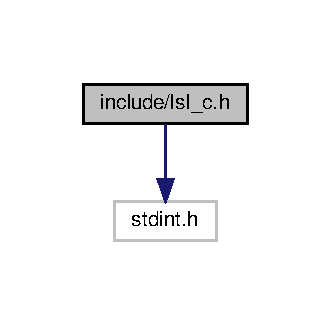
\includegraphics[width=159pt]{de/d29/lsl__c_8h__incl}
\end{center}
\end{figure}
This graph shows which files directly or indirectly include this file\+:\nopagebreak
\begin{figure}[H]
\begin{center}
\leavevmode
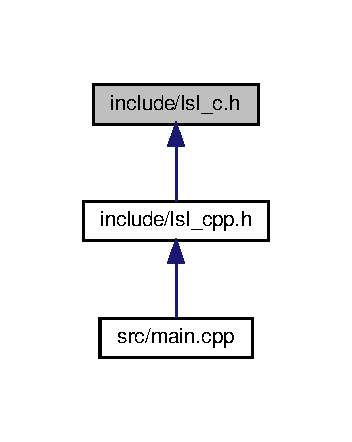
\includegraphics[width=169pt]{df/d9b/lsl__c_8h__dep__incl}
\end{center}
\end{figure}
\subsection*{Macros}
\begin{DoxyCompactItemize}
\item 
\#define \hyperlink{lsl__c_8h_aafd0ef1813e8be84a1420c4f1df64615}{L\+I\+B\+L\+S\+L\+\_\+\+C\+\_\+\+A\+PI}~\+\_\+\+\_\+attribute\+\_\+\+\_\+((visibility(\char`\"{}default\char`\"{})))
\item 
\#define \hyperlink{lsl__c_8h_ab46eddb74ca540d49497330b132dbff1}{L\+S\+L\+\_\+\+I\+R\+R\+E\+G\+U\+L\+A\+R\+\_\+\+R\+A\+TE}~0.\+0
\item 
\#define \hyperlink{lsl__c_8h_a5282bfa3df16b30eb308375a45062cfc}{L\+S\+L\+\_\+\+D\+E\+D\+U\+C\+E\+D\+\_\+\+T\+I\+M\+E\+S\+T\+A\+MP}~-\/1.\+0
\item 
\#define \hyperlink{lsl__c_8h_a0416859f36f40e91d12cd07aafb34eaa}{L\+S\+L\+\_\+\+F\+O\+R\+E\+V\+ER}~32000000.\+0
\item 
\#define \hyperlink{lsl__c_8h_ab94fcb1a355dbfc31f9dd3e0d699e6d6}{L\+S\+L\+\_\+\+N\+O\+\_\+\+P\+R\+E\+F\+E\+R\+E\+N\+CE}~0
\item 
\#define \hyperlink{lsl__c_8h_a8575e959edab9eb4be131982dd260acd}{L\+I\+B\+L\+S\+L\+\_\+\+C\+O\+M\+P\+I\+L\+E\+\_\+\+H\+E\+A\+D\+E\+R\+\_\+\+V\+E\+R\+S\+I\+ON}~= 113;
\item 
\#define \hyperlink{lsl__cpp_8h_a89d11cd08caa9cf3a4591d6b0f0a24c5}{L\+S\+L\+\_\+\+C\+\_\+H}
\item 
\#define \hyperlink{lsl__cpp_8h_aafd0ef1813e8be84a1420c4f1df64615}{L\+I\+B\+L\+S\+L\+\_\+\+C\+\_\+\+A\+PI}~\+\_\+\+\_\+attribute\+\_\+\+\_\+((visibility(\char`\"{}default\char`\"{})))
\item 
\#define \hyperlink{lsl__cpp_8h_ab46eddb74ca540d49497330b132dbff1}{L\+S\+L\+\_\+\+I\+R\+R\+E\+G\+U\+L\+A\+R\+\_\+\+R\+A\+TE}~0.\+0
\item 
\#define \hyperlink{lsl__cpp_8h_a5282bfa3df16b30eb308375a45062cfc}{L\+S\+L\+\_\+\+D\+E\+D\+U\+C\+E\+D\+\_\+\+T\+I\+M\+E\+S\+T\+A\+MP}~-\/1.\+0
\item 
\#define \hyperlink{lsl__cpp_8h_a0416859f36f40e91d12cd07aafb34eaa}{L\+S\+L\+\_\+\+F\+O\+R\+E\+V\+ER}~32000000.\+0
\item 
\#define \hyperlink{lsl__cpp_8h_ab94fcb1a355dbfc31f9dd3e0d699e6d6}{L\+S\+L\+\_\+\+N\+O\+\_\+\+P\+R\+E\+F\+E\+R\+E\+N\+CE}~0
\item 
\#define \hyperlink{lsl__cpp_8h_a8575e959edab9eb4be131982dd260acd}{L\+I\+B\+L\+S\+L\+\_\+\+C\+O\+M\+P\+I\+L\+E\+\_\+\+H\+E\+A\+D\+E\+R\+\_\+\+V\+E\+R\+S\+I\+ON}~= 113;
\end{DoxyCompactItemize}
\subsection*{Typedefs}
\begin{DoxyCompactItemize}
\item 
typedef struct lsl\+\_\+streaminfo\+\_\+struct\+\_\+ $\ast$ \hyperlink{lsl__c_8h_a6fd635c662a9c80840b53bd7c202499c}{lsl\+\_\+streaminfo}
\item 
typedef struct lsl\+\_\+outlet\+\_\+struct\+\_\+ $\ast$ \hyperlink{lsl__c_8h_aef1212b6b2cd3e3747fd6e433c30e395}{lsl\+\_\+outlet}
\item 
typedef struct lsl\+\_\+inlet\+\_\+struct\+\_\+ $\ast$ \hyperlink{lsl__c_8h_aff5474907fddf8b14300c79c9fda38e6}{lsl\+\_\+inlet}
\item 
typedef struct lsl\+\_\+xml\+\_\+ptr\+\_\+struct\+\_\+ $\ast$ \hyperlink{lsl__c_8h_ab174601268a7f0a9b60223510ba7d3b8}{lsl\+\_\+xml\+\_\+ptr}
\item 
typedef struct lsl\+\_\+continuous\+\_\+resolver\+\_\+ $\ast$ \hyperlink{lsl__c_8h_a78b224e996f3a73b35f4c5d73d721366}{lsl\+\_\+continuous\+\_\+resolver}
\end{DoxyCompactItemize}
\subsection*{Enumerations}
\begin{DoxyCompactItemize}
\item 
enum \hyperlink{lsl__c_8h_ad346feb32bddd136c3f7797e45047754}{lsl\+\_\+channel\+\_\+format\+\_\+t} \{ \newline
\hyperlink{lsl__c_8h_ad346feb32bddd136c3f7797e45047754a0548a6d8aa4e05f6195b7d7667b1a708}{cft\+\_\+float32} = 1, 
\hyperlink{lsl__c_8h_ad346feb32bddd136c3f7797e45047754a3286e5e97a2240d0fc4375e6eaf26291}{cft\+\_\+double64} = 2, 
\hyperlink{lsl__c_8h_ad346feb32bddd136c3f7797e45047754a8353906afd3439e2f9dc504f571a724d}{cft\+\_\+string} = 3, 
\hyperlink{lsl__c_8h_ad346feb32bddd136c3f7797e45047754a2048ca1d716016ec3439711eaf352652}{cft\+\_\+int32} = 4, 
\newline
\hyperlink{lsl__c_8h_ad346feb32bddd136c3f7797e45047754ab0af40c86cf7de7ff94f52006f924f3b}{cft\+\_\+int16} = 5, 
\hyperlink{lsl__c_8h_ad346feb32bddd136c3f7797e45047754a1b18c0e17a470b9e3bcff23cf49b8d6b}{cft\+\_\+int8} = 6, 
\hyperlink{lsl__c_8h_ad346feb32bddd136c3f7797e45047754a90aad2d18937be799aca56fe80794aa5}{cft\+\_\+int64} = 7, 
\hyperlink{lsl__c_8h_ad346feb32bddd136c3f7797e45047754a0cbaf0c7054a57713970489abab7fb85}{cft\+\_\+undefined} = 0
 \}
\item 
enum \hyperlink{lsl__c_8h_a9246faefd09869849b726df268042333}{lsl\+\_\+processing\+\_\+options\+\_\+t} \{ \newline
\hyperlink{lsl__c_8h_a9246faefd09869849b726df268042333a10e08b294e3583a6e1892da753137445}{proc\+\_\+none} = 0, 
\hyperlink{lsl__c_8h_a9246faefd09869849b726df268042333ae6bdb3d07024fa143a22417546496828}{proc\+\_\+clocksync} = 1, 
\hyperlink{lsl__c_8h_a9246faefd09869849b726df268042333a21f46ef0bbdba358fabe116ae1559c87}{proc\+\_\+dejitter} = 2, 
\hyperlink{lsl__c_8h_a9246faefd09869849b726df268042333ad36e527d8a75f2ef42d48311bbd605c7}{proc\+\_\+monotonize} = 4, 
\newline
\hyperlink{lsl__c_8h_a9246faefd09869849b726df268042333af3444351bc66b5a0a8a758774de84438}{proc\+\_\+threadsafe} = 8, 
\hyperlink{lsl__c_8h_a9246faefd09869849b726df268042333ae75b6de5e0af2a7c1377c11fafefbb02}{proc\+\_\+\+A\+LL} = 1$\vert$2$\vert$4$\vert$8
 \}
\item 
enum \hyperlink{lsl__c_8h_a0be58f7d496eb06924ee1825219c6e50}{lsl\+\_\+error\+\_\+code\+\_\+t} \{ \newline
\hyperlink{lsl__c_8h_a0be58f7d496eb06924ee1825219c6e50ae6bc06b8e33c37c36c1edae45b4778c1}{lsl\+\_\+no\+\_\+error} = 0, 
\hyperlink{lsl__c_8h_a0be58f7d496eb06924ee1825219c6e50a41650b5604c0b7392b79d383a7f59a68}{lsl\+\_\+timeout\+\_\+error} = -\/1, 
\hyperlink{lsl__c_8h_a0be58f7d496eb06924ee1825219c6e50aa463db40788d297314191e0b41081feb}{lsl\+\_\+lost\+\_\+error} = -\/2, 
\hyperlink{lsl__c_8h_a0be58f7d496eb06924ee1825219c6e50ad4626ba223d8c0b1535074752b0a0463}{lsl\+\_\+argument\+\_\+error} = -\/3, 
\newline
\hyperlink{lsl__c_8h_a0be58f7d496eb06924ee1825219c6e50a600b03c28953fa600d6c4e544a14fd99}{lsl\+\_\+internal\+\_\+error} = -\/4
 \}
\end{DoxyCompactItemize}
\subsection*{Functions}
\begin{DoxyCompactItemize}
\item 
\hyperlink{lsl__cpp_8h_aafd0ef1813e8be84a1420c4f1df64615}{L\+I\+B\+L\+S\+L\+\_\+\+C\+\_\+\+A\+PI} int32\+\_\+t \hyperlink{lsl__c_8h_a41474948cae5d78c552e3a98d5ecd5bc}{lsl\+\_\+protocol\+\_\+version} ()
\item 
\hyperlink{lsl__cpp_8h_aafd0ef1813e8be84a1420c4f1df64615}{L\+I\+B\+L\+S\+L\+\_\+\+C\+\_\+\+A\+PI} int32\+\_\+t \hyperlink{lsl__c_8h_a43f78dccab0a194c987b357a870e9fae}{lsl\+\_\+library\+\_\+version} ()
\item 
\hyperlink{lsl__cpp_8h_aafd0ef1813e8be84a1420c4f1df64615}{L\+I\+B\+L\+S\+L\+\_\+\+C\+\_\+\+A\+PI} const char $\ast$ \hyperlink{lsl__c_8h_ab5f5986ebe4bbf87d97d299b0c1213ea}{lsl\+\_\+library\+\_\+info} ()
\item 
\hyperlink{lsl__cpp_8h_aafd0ef1813e8be84a1420c4f1df64615}{L\+I\+B\+L\+S\+L\+\_\+\+C\+\_\+\+A\+PI} double \hyperlink{lsl__c_8h_ab5830dfa3831a239eabae33504633849}{lsl\+\_\+local\+\_\+clock} ()
\item 
\hyperlink{lsl__cpp_8h_aafd0ef1813e8be84a1420c4f1df64615}{L\+I\+B\+L\+S\+L\+\_\+\+C\+\_\+\+A\+PI} int32\+\_\+t \hyperlink{lsl__c_8h_ac9b53eec106d81130b5aa2341ecf8bd2}{lsl\+\_\+resolve\+\_\+all} (\hyperlink{lsl__c_8h_a6fd635c662a9c80840b53bd7c202499c}{lsl\+\_\+streaminfo} $\ast$buffer, uint32\+\_\+t buffer\+\_\+elements, double wait\+\_\+time)
\item 
\hyperlink{lsl__cpp_8h_aafd0ef1813e8be84a1420c4f1df64615}{L\+I\+B\+L\+S\+L\+\_\+\+C\+\_\+\+A\+PI} int32\+\_\+t \hyperlink{lsl__c_8h_ac704c51be54e926f6dcc8dc7d04d8b8b}{lsl\+\_\+resolve\+\_\+byprop} (\hyperlink{lsl__c_8h_a6fd635c662a9c80840b53bd7c202499c}{lsl\+\_\+streaminfo} $\ast$buffer, uint32\+\_\+t buffer\+\_\+elements, const char $\ast$prop, const char $\ast$value, int32\+\_\+t minimum, double timeout)
\item 
\hyperlink{lsl__cpp_8h_aafd0ef1813e8be84a1420c4f1df64615}{L\+I\+B\+L\+S\+L\+\_\+\+C\+\_\+\+A\+PI} int32\+\_\+t \hyperlink{lsl__c_8h_a0effb3c0c3ea96a144d3f13265d7d588}{lsl\+\_\+resolve\+\_\+bypred} (\hyperlink{lsl__c_8h_a6fd635c662a9c80840b53bd7c202499c}{lsl\+\_\+streaminfo} $\ast$buffer, uint32\+\_\+t buffer\+\_\+elements, const char $\ast$pred, int32\+\_\+t minimum, double timeout)
\item 
\hyperlink{lsl__cpp_8h_aafd0ef1813e8be84a1420c4f1df64615}{L\+I\+B\+L\+S\+L\+\_\+\+C\+\_\+\+A\+PI} void \hyperlink{lsl__c_8h_addeff0a60f446e7f43770eb1f5e30f84}{lsl\+\_\+destroy\+\_\+string} (char $\ast$s)
\item 
\hyperlink{lsl__cpp_8h_aafd0ef1813e8be84a1420c4f1df64615}{L\+I\+B\+L\+S\+L\+\_\+\+C\+\_\+\+A\+PI} \hyperlink{lsl__c_8h_a6fd635c662a9c80840b53bd7c202499c}{lsl\+\_\+streaminfo} \hyperlink{lsl__c_8h_ad84630a74d54a33c972daa18feb78c9d}{lsl\+\_\+create\+\_\+streaminfo} (const char $\ast$name, const char $\ast$type, int32\+\_\+t channel\+\_\+count, double nominal\+\_\+srate, \hyperlink{lsl__c_8h_ad346feb32bddd136c3f7797e45047754}{lsl\+\_\+channel\+\_\+format\+\_\+t} channel\+\_\+format, const char $\ast$source\+\_\+id)
\item 
\hyperlink{lsl__cpp_8h_aafd0ef1813e8be84a1420c4f1df64615}{L\+I\+B\+L\+S\+L\+\_\+\+C\+\_\+\+A\+PI} void \hyperlink{lsl__c_8h_aaa63607a0162e2ab9e62dffc7874d716}{lsl\+\_\+destroy\+\_\+streaminfo} (\hyperlink{lsl__c_8h_a6fd635c662a9c80840b53bd7c202499c}{lsl\+\_\+streaminfo} info)
\item 
\hyperlink{lsl__cpp_8h_aafd0ef1813e8be84a1420c4f1df64615}{L\+I\+B\+L\+S\+L\+\_\+\+C\+\_\+\+A\+PI} \hyperlink{lsl__c_8h_a6fd635c662a9c80840b53bd7c202499c}{lsl\+\_\+streaminfo} \hyperlink{lsl__c_8h_a4514f8ed63874d11e756a59d99b0326d}{lsl\+\_\+copy\+\_\+streaminfo} (\hyperlink{lsl__c_8h_a6fd635c662a9c80840b53bd7c202499c}{lsl\+\_\+streaminfo} info)
\item 
\hyperlink{lsl__cpp_8h_aafd0ef1813e8be84a1420c4f1df64615}{L\+I\+B\+L\+S\+L\+\_\+\+C\+\_\+\+A\+PI} const char $\ast$ \hyperlink{lsl__c_8h_a86691767b61f0731a3e0668efd42c224}{lsl\+\_\+get\+\_\+name} (\hyperlink{lsl__c_8h_a6fd635c662a9c80840b53bd7c202499c}{lsl\+\_\+streaminfo} info)
\item 
\hyperlink{lsl__cpp_8h_aafd0ef1813e8be84a1420c4f1df64615}{L\+I\+B\+L\+S\+L\+\_\+\+C\+\_\+\+A\+PI} const char $\ast$ \hyperlink{lsl__c_8h_a8f6958b1292ad3b59157c290bfce552d}{lsl\+\_\+get\+\_\+type} (\hyperlink{lsl__c_8h_a6fd635c662a9c80840b53bd7c202499c}{lsl\+\_\+streaminfo} info)
\item 
\hyperlink{lsl__cpp_8h_aafd0ef1813e8be84a1420c4f1df64615}{L\+I\+B\+L\+S\+L\+\_\+\+C\+\_\+\+A\+PI} int32\+\_\+t \hyperlink{lsl__c_8h_a5a736ebd5f1fbbd26dc5f66dcdd4edd1}{lsl\+\_\+get\+\_\+channel\+\_\+count} (\hyperlink{lsl__c_8h_a6fd635c662a9c80840b53bd7c202499c}{lsl\+\_\+streaminfo} info)
\item 
\hyperlink{lsl__cpp_8h_aafd0ef1813e8be84a1420c4f1df64615}{L\+I\+B\+L\+S\+L\+\_\+\+C\+\_\+\+A\+PI} double \hyperlink{lsl__c_8h_a52b66d7a75574d98e8709d1734fdd113}{lsl\+\_\+get\+\_\+nominal\+\_\+srate} (\hyperlink{lsl__c_8h_a6fd635c662a9c80840b53bd7c202499c}{lsl\+\_\+streaminfo} info)
\item 
\hyperlink{lsl__cpp_8h_aafd0ef1813e8be84a1420c4f1df64615}{L\+I\+B\+L\+S\+L\+\_\+\+C\+\_\+\+A\+PI} \hyperlink{lsl__c_8h_ad346feb32bddd136c3f7797e45047754}{lsl\+\_\+channel\+\_\+format\+\_\+t} \hyperlink{lsl__c_8h_aa85ef584982dd371ca580e5103cef633}{lsl\+\_\+get\+\_\+channel\+\_\+format} (\hyperlink{lsl__c_8h_a6fd635c662a9c80840b53bd7c202499c}{lsl\+\_\+streaminfo} info)
\item 
\hyperlink{lsl__cpp_8h_aafd0ef1813e8be84a1420c4f1df64615}{L\+I\+B\+L\+S\+L\+\_\+\+C\+\_\+\+A\+PI} const char $\ast$ \hyperlink{lsl__c_8h_a98b8df791e7e9d415098aafcb06b3d93}{lsl\+\_\+get\+\_\+source\+\_\+id} (\hyperlink{lsl__c_8h_a6fd635c662a9c80840b53bd7c202499c}{lsl\+\_\+streaminfo} info)
\item 
\hyperlink{lsl__cpp_8h_aafd0ef1813e8be84a1420c4f1df64615}{L\+I\+B\+L\+S\+L\+\_\+\+C\+\_\+\+A\+PI} int32\+\_\+t \hyperlink{lsl__c_8h_a4c8de5b8ac7e0c9400082a90b398a9e6}{lsl\+\_\+get\+\_\+version} (\hyperlink{lsl__c_8h_a6fd635c662a9c80840b53bd7c202499c}{lsl\+\_\+streaminfo} info)
\item 
\hyperlink{lsl__cpp_8h_aafd0ef1813e8be84a1420c4f1df64615}{L\+I\+B\+L\+S\+L\+\_\+\+C\+\_\+\+A\+PI} double \hyperlink{lsl__c_8h_aae3594f14dbcf50ea012d89403f5d57c}{lsl\+\_\+get\+\_\+created\+\_\+at} (\hyperlink{lsl__c_8h_a6fd635c662a9c80840b53bd7c202499c}{lsl\+\_\+streaminfo} info)
\item 
\hyperlink{lsl__cpp_8h_aafd0ef1813e8be84a1420c4f1df64615}{L\+I\+B\+L\+S\+L\+\_\+\+C\+\_\+\+A\+PI} const char $\ast$ \hyperlink{lsl__c_8h_a381b60fcb6379eacda3276218751290c}{lsl\+\_\+get\+\_\+uid} (\hyperlink{lsl__c_8h_a6fd635c662a9c80840b53bd7c202499c}{lsl\+\_\+streaminfo} info)
\item 
\hyperlink{lsl__cpp_8h_aafd0ef1813e8be84a1420c4f1df64615}{L\+I\+B\+L\+S\+L\+\_\+\+C\+\_\+\+A\+PI} const char $\ast$ \hyperlink{lsl__c_8h_a66b17ecf6f20b0d5d8f1ed78080515ba}{lsl\+\_\+get\+\_\+session\+\_\+id} (\hyperlink{lsl__c_8h_a6fd635c662a9c80840b53bd7c202499c}{lsl\+\_\+streaminfo} info)
\item 
\hyperlink{lsl__cpp_8h_aafd0ef1813e8be84a1420c4f1df64615}{L\+I\+B\+L\+S\+L\+\_\+\+C\+\_\+\+A\+PI} const char $\ast$ \hyperlink{lsl__c_8h_ab517961395988205f230c14c94cf9506}{lsl\+\_\+get\+\_\+hostname} (\hyperlink{lsl__c_8h_a6fd635c662a9c80840b53bd7c202499c}{lsl\+\_\+streaminfo} info)
\item 
\hyperlink{lsl__cpp_8h_aafd0ef1813e8be84a1420c4f1df64615}{L\+I\+B\+L\+S\+L\+\_\+\+C\+\_\+\+A\+PI} \hyperlink{lsl__c_8h_ab174601268a7f0a9b60223510ba7d3b8}{lsl\+\_\+xml\+\_\+ptr} \hyperlink{lsl__c_8h_afef7ba2a6124b285f4568af0cf200420}{lsl\+\_\+get\+\_\+desc} (\hyperlink{lsl__c_8h_a6fd635c662a9c80840b53bd7c202499c}{lsl\+\_\+streaminfo} info)
\item 
\hyperlink{lsl__cpp_8h_aafd0ef1813e8be84a1420c4f1df64615}{L\+I\+B\+L\+S\+L\+\_\+\+C\+\_\+\+A\+PI} char $\ast$ \hyperlink{lsl__c_8h_a620092f125b45938623229fee3a366f9}{lsl\+\_\+get\+\_\+xml} (\hyperlink{lsl__c_8h_a6fd635c662a9c80840b53bd7c202499c}{lsl\+\_\+streaminfo} info)
\item 
\hyperlink{lsl__cpp_8h_aafd0ef1813e8be84a1420c4f1df64615}{L\+I\+B\+L\+S\+L\+\_\+\+C\+\_\+\+A\+PI} int32\+\_\+t \hyperlink{lsl__c_8h_ace8095ccb59a3857b0ff42511c72ff9a}{lsl\+\_\+get\+\_\+channel\+\_\+bytes} (\hyperlink{lsl__c_8h_a6fd635c662a9c80840b53bd7c202499c}{lsl\+\_\+streaminfo} info)
\begin{DoxyCompactList}\small\item\em Number of bytes occupied by a channel (0 for string-\/typed channels). \end{DoxyCompactList}\item 
\hyperlink{lsl__cpp_8h_aafd0ef1813e8be84a1420c4f1df64615}{L\+I\+B\+L\+S\+L\+\_\+\+C\+\_\+\+A\+PI} int32\+\_\+t \hyperlink{lsl__c_8h_ac0ce4de263cd07fc4e3b1808e784693f}{lsl\+\_\+get\+\_\+sample\+\_\+bytes} (\hyperlink{lsl__c_8h_a6fd635c662a9c80840b53bd7c202499c}{lsl\+\_\+streaminfo} info)
\begin{DoxyCompactList}\small\item\em Number of bytes occupied by a sample (0 for string-\/typed channels). \end{DoxyCompactList}\item 
\hyperlink{lsl__cpp_8h_aafd0ef1813e8be84a1420c4f1df64615}{L\+I\+B\+L\+S\+L\+\_\+\+C\+\_\+\+A\+PI} int \hyperlink{lsl__c_8h_a8e0d0447b9598bfe0e46a6166de51cc3}{lsl\+\_\+stream\+\_\+info\+\_\+matches\+\_\+query} (\hyperlink{lsl__c_8h_a6fd635c662a9c80840b53bd7c202499c}{lsl\+\_\+streaminfo} info, const char $\ast$query)
\item 
\hyperlink{lsl__cpp_8h_aafd0ef1813e8be84a1420c4f1df64615}{L\+I\+B\+L\+S\+L\+\_\+\+C\+\_\+\+A\+PI} \hyperlink{lsl__c_8h_a6fd635c662a9c80840b53bd7c202499c}{lsl\+\_\+streaminfo} \hyperlink{lsl__c_8h_a2d42a5d991505811d98ba04c6319f41b}{lsl\+\_\+streaminfo\+\_\+from\+\_\+xml} (const char $\ast$xml)
\begin{DoxyCompactList}\small\item\em Create a streaminfo object from an X\+ML representation. \end{DoxyCompactList}\item 
\hyperlink{lsl__cpp_8h_aafd0ef1813e8be84a1420c4f1df64615}{L\+I\+B\+L\+S\+L\+\_\+\+C\+\_\+\+A\+PI} \hyperlink{lsl__c_8h_aef1212b6b2cd3e3747fd6e433c30e395}{lsl\+\_\+outlet} \hyperlink{lsl__c_8h_a22a7097dedf222014e6b878f3870b0fa}{lsl\+\_\+create\+\_\+outlet} (\hyperlink{lsl__c_8h_a6fd635c662a9c80840b53bd7c202499c}{lsl\+\_\+streaminfo} info, int32\+\_\+t chunk\+\_\+size, int32\+\_\+t max\+\_\+buffered)
\item 
\hyperlink{lsl__cpp_8h_aafd0ef1813e8be84a1420c4f1df64615}{L\+I\+B\+L\+S\+L\+\_\+\+C\+\_\+\+A\+PI} void \hyperlink{lsl__c_8h_a0588f316a9e406e61f1507d8f756529f}{lsl\+\_\+destroy\+\_\+outlet} (\hyperlink{lsl__c_8h_aef1212b6b2cd3e3747fd6e433c30e395}{lsl\+\_\+outlet} out)
\item 
\hyperlink{lsl__cpp_8h_aafd0ef1813e8be84a1420c4f1df64615}{L\+I\+B\+L\+S\+L\+\_\+\+C\+\_\+\+A\+PI} int32\+\_\+t \hyperlink{lsl__c_8h_aad62f3e27452d2944cd8cb443fc11741}{lsl\+\_\+push\+\_\+sample\+\_\+f} (\hyperlink{lsl__c_8h_aef1212b6b2cd3e3747fd6e433c30e395}{lsl\+\_\+outlet} out, const float $\ast$data)
\item 
\hyperlink{lsl__cpp_8h_aafd0ef1813e8be84a1420c4f1df64615}{L\+I\+B\+L\+S\+L\+\_\+\+C\+\_\+\+A\+PI} int32\+\_\+t \hyperlink{lsl__c_8h_af0f78c4ea3b891919666047bf1bdbc90}{lsl\+\_\+push\+\_\+sample\+\_\+ft} (\hyperlink{lsl__c_8h_aef1212b6b2cd3e3747fd6e433c30e395}{lsl\+\_\+outlet} out, const float $\ast$data, double timestamp)
\item 
\hyperlink{lsl__cpp_8h_aafd0ef1813e8be84a1420c4f1df64615}{L\+I\+B\+L\+S\+L\+\_\+\+C\+\_\+\+A\+PI} int32\+\_\+t \hyperlink{lsl__c_8h_a03d1dce2aaa12d3787d0f501c50fe06f}{lsl\+\_\+push\+\_\+sample\+\_\+ftp} (\hyperlink{lsl__c_8h_aef1212b6b2cd3e3747fd6e433c30e395}{lsl\+\_\+outlet} out, const float $\ast$data, double timestamp, int32\+\_\+t pushthrough)
\item 
\hyperlink{lsl__cpp_8h_aafd0ef1813e8be84a1420c4f1df64615}{L\+I\+B\+L\+S\+L\+\_\+\+C\+\_\+\+A\+PI} int32\+\_\+t \hyperlink{lsl__c_8h_ae44e19988a72b422344711d5017cb420}{lsl\+\_\+push\+\_\+sample\+\_\+d} (\hyperlink{lsl__c_8h_aef1212b6b2cd3e3747fd6e433c30e395}{lsl\+\_\+outlet} out, const double $\ast$data)
\item 
\hyperlink{lsl__cpp_8h_aafd0ef1813e8be84a1420c4f1df64615}{L\+I\+B\+L\+S\+L\+\_\+\+C\+\_\+\+A\+PI} int32\+\_\+t \hyperlink{lsl__c_8h_a224bb668fb637074adbcf301208c3052}{lsl\+\_\+push\+\_\+sample\+\_\+dt} (\hyperlink{lsl__c_8h_aef1212b6b2cd3e3747fd6e433c30e395}{lsl\+\_\+outlet} out, const double $\ast$data, double timestamp)
\item 
\hyperlink{lsl__cpp_8h_aafd0ef1813e8be84a1420c4f1df64615}{L\+I\+B\+L\+S\+L\+\_\+\+C\+\_\+\+A\+PI} int32\+\_\+t \hyperlink{lsl__c_8h_af3604739246b9b9175b990eb74fbe183}{lsl\+\_\+push\+\_\+sample\+\_\+dtp} (\hyperlink{lsl__c_8h_aef1212b6b2cd3e3747fd6e433c30e395}{lsl\+\_\+outlet} out, const double $\ast$data, double timestamp, int32\+\_\+t pushthrough)
\item 
\hyperlink{lsl__cpp_8h_aafd0ef1813e8be84a1420c4f1df64615}{L\+I\+B\+L\+S\+L\+\_\+\+C\+\_\+\+A\+PI} int32\+\_\+t \hyperlink{lsl__c_8h_a1a0f09509cfc4e87346a15216fa852c6}{lsl\+\_\+push\+\_\+sample\+\_\+l} (\hyperlink{lsl__c_8h_aef1212b6b2cd3e3747fd6e433c30e395}{lsl\+\_\+outlet} out, const long $\ast$data)
\item 
\hyperlink{lsl__cpp_8h_aafd0ef1813e8be84a1420c4f1df64615}{L\+I\+B\+L\+S\+L\+\_\+\+C\+\_\+\+A\+PI} int32\+\_\+t \hyperlink{lsl__c_8h_a6e502508ea597c9f9a4a129cddd4e799}{lsl\+\_\+push\+\_\+sample\+\_\+lt} (\hyperlink{lsl__c_8h_aef1212b6b2cd3e3747fd6e433c30e395}{lsl\+\_\+outlet} out, const long $\ast$data, double timestamp)
\item 
\hyperlink{lsl__cpp_8h_aafd0ef1813e8be84a1420c4f1df64615}{L\+I\+B\+L\+S\+L\+\_\+\+C\+\_\+\+A\+PI} int32\+\_\+t \hyperlink{lsl__c_8h_ab3acfb108aa4260818588e75d61307c2}{lsl\+\_\+push\+\_\+sample\+\_\+ltp} (\hyperlink{lsl__c_8h_aef1212b6b2cd3e3747fd6e433c30e395}{lsl\+\_\+outlet} out, const long $\ast$data, double timestamp, int32\+\_\+t pushthrough)
\item 
\hyperlink{lsl__cpp_8h_aafd0ef1813e8be84a1420c4f1df64615}{L\+I\+B\+L\+S\+L\+\_\+\+C\+\_\+\+A\+PI} int32\+\_\+t \hyperlink{lsl__c_8h_aa08759dc9e3d361fbc26557fc7a42279}{lsl\+\_\+push\+\_\+sample\+\_\+i} (\hyperlink{lsl__c_8h_aef1212b6b2cd3e3747fd6e433c30e395}{lsl\+\_\+outlet} out, const int32\+\_\+t $\ast$data)
\item 
\hyperlink{lsl__cpp_8h_aafd0ef1813e8be84a1420c4f1df64615}{L\+I\+B\+L\+S\+L\+\_\+\+C\+\_\+\+A\+PI} int32\+\_\+t \hyperlink{lsl__c_8h_a2a69d88399fded37ac1f83a76255b464}{lsl\+\_\+push\+\_\+sample\+\_\+it} (\hyperlink{lsl__c_8h_aef1212b6b2cd3e3747fd6e433c30e395}{lsl\+\_\+outlet} out, const int32\+\_\+t $\ast$data, double timestamp)
\item 
\hyperlink{lsl__cpp_8h_aafd0ef1813e8be84a1420c4f1df64615}{L\+I\+B\+L\+S\+L\+\_\+\+C\+\_\+\+A\+PI} int32\+\_\+t \hyperlink{lsl__c_8h_a2b4dd3c7f41dd81766cdbfe7048fabd9}{lsl\+\_\+push\+\_\+sample\+\_\+itp} (\hyperlink{lsl__c_8h_aef1212b6b2cd3e3747fd6e433c30e395}{lsl\+\_\+outlet} out, const int32\+\_\+t $\ast$data, double timestamp, int32\+\_\+t pushthrough)
\item 
\hyperlink{lsl__cpp_8h_aafd0ef1813e8be84a1420c4f1df64615}{L\+I\+B\+L\+S\+L\+\_\+\+C\+\_\+\+A\+PI} int32\+\_\+t \hyperlink{lsl__c_8h_abc5a012ac671893b58d38d81b4433520}{lsl\+\_\+push\+\_\+sample\+\_\+s} (\hyperlink{lsl__c_8h_aef1212b6b2cd3e3747fd6e433c30e395}{lsl\+\_\+outlet} out, const int16\+\_\+t $\ast$data)
\item 
\hyperlink{lsl__cpp_8h_aafd0ef1813e8be84a1420c4f1df64615}{L\+I\+B\+L\+S\+L\+\_\+\+C\+\_\+\+A\+PI} int32\+\_\+t \hyperlink{lsl__c_8h_a3b6c842b79ce6040d5fae9ee5b06a705}{lsl\+\_\+push\+\_\+sample\+\_\+st} (\hyperlink{lsl__c_8h_aef1212b6b2cd3e3747fd6e433c30e395}{lsl\+\_\+outlet} out, const int16\+\_\+t $\ast$data, double timestamp)
\item 
\hyperlink{lsl__cpp_8h_aafd0ef1813e8be84a1420c4f1df64615}{L\+I\+B\+L\+S\+L\+\_\+\+C\+\_\+\+A\+PI} int32\+\_\+t \hyperlink{lsl__c_8h_a9a8d74a7fef9cdf68bd3a1ecf76109fa}{lsl\+\_\+push\+\_\+sample\+\_\+stp} (\hyperlink{lsl__c_8h_aef1212b6b2cd3e3747fd6e433c30e395}{lsl\+\_\+outlet} out, const int16\+\_\+t $\ast$data, double timestamp, int32\+\_\+t pushthrough)
\item 
\hyperlink{lsl__cpp_8h_aafd0ef1813e8be84a1420c4f1df64615}{L\+I\+B\+L\+S\+L\+\_\+\+C\+\_\+\+A\+PI} int32\+\_\+t \hyperlink{lsl__c_8h_abac187f58d92db9130d18139d72064a9}{lsl\+\_\+push\+\_\+sample\+\_\+c} (\hyperlink{lsl__c_8h_aef1212b6b2cd3e3747fd6e433c30e395}{lsl\+\_\+outlet} out, const char $\ast$data)
\item 
\hyperlink{lsl__cpp_8h_aafd0ef1813e8be84a1420c4f1df64615}{L\+I\+B\+L\+S\+L\+\_\+\+C\+\_\+\+A\+PI} int32\+\_\+t \hyperlink{lsl__c_8h_a3d8187c61f5dd8471e5c00610103cdee}{lsl\+\_\+push\+\_\+sample\+\_\+ct} (\hyperlink{lsl__c_8h_aef1212b6b2cd3e3747fd6e433c30e395}{lsl\+\_\+outlet} out, const char $\ast$data, double timestamp)
\item 
\hyperlink{lsl__cpp_8h_aafd0ef1813e8be84a1420c4f1df64615}{L\+I\+B\+L\+S\+L\+\_\+\+C\+\_\+\+A\+PI} int32\+\_\+t \hyperlink{lsl__c_8h_a79cca3f3f75ae677d973758b8cfd8295}{lsl\+\_\+push\+\_\+sample\+\_\+ctp} (\hyperlink{lsl__c_8h_aef1212b6b2cd3e3747fd6e433c30e395}{lsl\+\_\+outlet} out, const char $\ast$data, double timestamp, int32\+\_\+t pushthrough)
\item 
\hyperlink{lsl__cpp_8h_aafd0ef1813e8be84a1420c4f1df64615}{L\+I\+B\+L\+S\+L\+\_\+\+C\+\_\+\+A\+PI} int32\+\_\+t \hyperlink{lsl__c_8h_a70a523aded3aaa76ba81aeaebb22e8df}{lsl\+\_\+push\+\_\+sample\+\_\+str} (\hyperlink{lsl__c_8h_aef1212b6b2cd3e3747fd6e433c30e395}{lsl\+\_\+outlet} out, const char $\ast$$\ast$data)
\item 
\hyperlink{lsl__cpp_8h_aafd0ef1813e8be84a1420c4f1df64615}{L\+I\+B\+L\+S\+L\+\_\+\+C\+\_\+\+A\+PI} int32\+\_\+t \hyperlink{lsl__c_8h_a281c387af4465c231abb4daed25431b3}{lsl\+\_\+push\+\_\+sample\+\_\+strt} (\hyperlink{lsl__c_8h_aef1212b6b2cd3e3747fd6e433c30e395}{lsl\+\_\+outlet} out, const char $\ast$$\ast$data, double timestamp)
\item 
\hyperlink{lsl__cpp_8h_aafd0ef1813e8be84a1420c4f1df64615}{L\+I\+B\+L\+S\+L\+\_\+\+C\+\_\+\+A\+PI} int32\+\_\+t \hyperlink{lsl__c_8h_a72938aad4ca7af001b8a3d8d2d64fa2d}{lsl\+\_\+push\+\_\+sample\+\_\+strtp} (\hyperlink{lsl__c_8h_aef1212b6b2cd3e3747fd6e433c30e395}{lsl\+\_\+outlet} out, const char $\ast$$\ast$data, double timestamp, int32\+\_\+t pushthrough)
\item 
\hyperlink{lsl__cpp_8h_aafd0ef1813e8be84a1420c4f1df64615}{L\+I\+B\+L\+S\+L\+\_\+\+C\+\_\+\+A\+PI} int32\+\_\+t \hyperlink{lsl__c_8h_a2e1505acff3a75a3e93a60ef4684456b}{lsl\+\_\+push\+\_\+sample\+\_\+buf} (\hyperlink{lsl__c_8h_aef1212b6b2cd3e3747fd6e433c30e395}{lsl\+\_\+outlet} out, const char $\ast$$\ast$data, const uint32\+\_\+t $\ast$lengths)
\item 
\hyperlink{lsl__cpp_8h_aafd0ef1813e8be84a1420c4f1df64615}{L\+I\+B\+L\+S\+L\+\_\+\+C\+\_\+\+A\+PI} int32\+\_\+t \hyperlink{lsl__c_8h_a8b8ed17844fa3b269ac65b51c3cac7c5}{lsl\+\_\+push\+\_\+sample\+\_\+buft} (\hyperlink{lsl__c_8h_aef1212b6b2cd3e3747fd6e433c30e395}{lsl\+\_\+outlet} out, const char $\ast$$\ast$data, const uint32\+\_\+t $\ast$lengths, double timestamp)
\item 
\hyperlink{lsl__cpp_8h_aafd0ef1813e8be84a1420c4f1df64615}{L\+I\+B\+L\+S\+L\+\_\+\+C\+\_\+\+A\+PI} int32\+\_\+t \hyperlink{lsl__c_8h_aa9716749d011b4f5c74e3eb4b7f86e6b}{lsl\+\_\+push\+\_\+sample\+\_\+buftp} (\hyperlink{lsl__c_8h_aef1212b6b2cd3e3747fd6e433c30e395}{lsl\+\_\+outlet} out, const char $\ast$$\ast$data, const uint32\+\_\+t $\ast$lengths, double timestamp, int32\+\_\+t pushthrough)
\item 
\hyperlink{lsl__cpp_8h_aafd0ef1813e8be84a1420c4f1df64615}{L\+I\+B\+L\+S\+L\+\_\+\+C\+\_\+\+A\+PI} int32\+\_\+t \hyperlink{lsl__c_8h_a9af4120da145ae6ebb904ad0b3bc1b43}{lsl\+\_\+push\+\_\+sample\+\_\+v} (\hyperlink{lsl__c_8h_aef1212b6b2cd3e3747fd6e433c30e395}{lsl\+\_\+outlet} out, const void $\ast$data)
\item 
\hyperlink{lsl__cpp_8h_aafd0ef1813e8be84a1420c4f1df64615}{L\+I\+B\+L\+S\+L\+\_\+\+C\+\_\+\+A\+PI} int32\+\_\+t \hyperlink{lsl__c_8h_a32e4ed2d5e4d064460f88d06fdc0b2d8}{lsl\+\_\+push\+\_\+sample\+\_\+vt} (\hyperlink{lsl__c_8h_aef1212b6b2cd3e3747fd6e433c30e395}{lsl\+\_\+outlet} out, const void $\ast$data, double timestamp)
\item 
\hyperlink{lsl__cpp_8h_aafd0ef1813e8be84a1420c4f1df64615}{L\+I\+B\+L\+S\+L\+\_\+\+C\+\_\+\+A\+PI} int32\+\_\+t \hyperlink{lsl__c_8h_ac6eb5ec72140ba4ae26c80112ccaac52}{lsl\+\_\+push\+\_\+sample\+\_\+vtp} (\hyperlink{lsl__c_8h_aef1212b6b2cd3e3747fd6e433c30e395}{lsl\+\_\+outlet} out, const void $\ast$data, double timestamp, int32\+\_\+t pushthrough)
\item 
\hyperlink{lsl__cpp_8h_aafd0ef1813e8be84a1420c4f1df64615}{L\+I\+B\+L\+S\+L\+\_\+\+C\+\_\+\+A\+PI} int32\+\_\+t \hyperlink{lsl__c_8h_a191171b4aae05abeae2d4172fc500795}{lsl\+\_\+push\+\_\+chunk\+\_\+f} (\hyperlink{lsl__c_8h_aef1212b6b2cd3e3747fd6e433c30e395}{lsl\+\_\+outlet} out, const float $\ast$data, unsigned long data\+\_\+elements)
\item 
\hyperlink{lsl__cpp_8h_aafd0ef1813e8be84a1420c4f1df64615}{L\+I\+B\+L\+S\+L\+\_\+\+C\+\_\+\+A\+PI} int32\+\_\+t \hyperlink{lsl__c_8h_a80f314d925564890ee64b1c2a699bdb0}{lsl\+\_\+push\+\_\+chunk\+\_\+ft} (\hyperlink{lsl__c_8h_aef1212b6b2cd3e3747fd6e433c30e395}{lsl\+\_\+outlet} out, const float $\ast$data, unsigned long data\+\_\+elements, double timestamp)
\item 
\hyperlink{lsl__cpp_8h_aafd0ef1813e8be84a1420c4f1df64615}{L\+I\+B\+L\+S\+L\+\_\+\+C\+\_\+\+A\+PI} int32\+\_\+t \hyperlink{lsl__c_8h_a91a947d9280a61e1e5e73d166a259385}{lsl\+\_\+push\+\_\+chunk\+\_\+ftp} (\hyperlink{lsl__c_8h_aef1212b6b2cd3e3747fd6e433c30e395}{lsl\+\_\+outlet} out, const float $\ast$data, unsigned long data\+\_\+elements, double timestamp, int32\+\_\+t pushthrough)
\item 
\hyperlink{lsl__cpp_8h_aafd0ef1813e8be84a1420c4f1df64615}{L\+I\+B\+L\+S\+L\+\_\+\+C\+\_\+\+A\+PI} int32\+\_\+t \hyperlink{lsl__c_8h_a4a39988b3987aa24d85f6f243c9cec9b}{lsl\+\_\+push\+\_\+chunk\+\_\+ftn} (\hyperlink{lsl__c_8h_aef1212b6b2cd3e3747fd6e433c30e395}{lsl\+\_\+outlet} out, const float $\ast$data, unsigned long data\+\_\+elements, const double $\ast$timestamps)
\item 
\hyperlink{lsl__cpp_8h_aafd0ef1813e8be84a1420c4f1df64615}{L\+I\+B\+L\+S\+L\+\_\+\+C\+\_\+\+A\+PI} int32\+\_\+t \hyperlink{lsl__c_8h_ac81be759a83eb75c357bfb820e83cd12}{lsl\+\_\+push\+\_\+chunk\+\_\+ftnp} (\hyperlink{lsl__c_8h_aef1212b6b2cd3e3747fd6e433c30e395}{lsl\+\_\+outlet} out, const float $\ast$data, unsigned long data\+\_\+elements, const double $\ast$timestamps, int32\+\_\+t pushthrough)
\item 
\hyperlink{lsl__cpp_8h_aafd0ef1813e8be84a1420c4f1df64615}{L\+I\+B\+L\+S\+L\+\_\+\+C\+\_\+\+A\+PI} int32\+\_\+t \hyperlink{lsl__c_8h_a227534e78fd4bbdf473ad7796da49377}{lsl\+\_\+push\+\_\+chunk\+\_\+d} (\hyperlink{lsl__c_8h_aef1212b6b2cd3e3747fd6e433c30e395}{lsl\+\_\+outlet} out, const double $\ast$data, unsigned long data\+\_\+elements)
\item 
\hyperlink{lsl__cpp_8h_aafd0ef1813e8be84a1420c4f1df64615}{L\+I\+B\+L\+S\+L\+\_\+\+C\+\_\+\+A\+PI} int32\+\_\+t \hyperlink{lsl__c_8h_a5a201ecffb48729d0eb0e51dba539a23}{lsl\+\_\+push\+\_\+chunk\+\_\+dt} (\hyperlink{lsl__c_8h_aef1212b6b2cd3e3747fd6e433c30e395}{lsl\+\_\+outlet} out, const double $\ast$data, unsigned long data\+\_\+elements, double timestamp)
\item 
\hyperlink{lsl__cpp_8h_aafd0ef1813e8be84a1420c4f1df64615}{L\+I\+B\+L\+S\+L\+\_\+\+C\+\_\+\+A\+PI} int32\+\_\+t \hyperlink{lsl__c_8h_a1e444e438b037d8a1363b1a74568976c}{lsl\+\_\+push\+\_\+chunk\+\_\+dtp} (\hyperlink{lsl__c_8h_aef1212b6b2cd3e3747fd6e433c30e395}{lsl\+\_\+outlet} out, const double $\ast$data, unsigned long data\+\_\+elements, double timestamp, int32\+\_\+t pushthrough)
\item 
\hyperlink{lsl__cpp_8h_aafd0ef1813e8be84a1420c4f1df64615}{L\+I\+B\+L\+S\+L\+\_\+\+C\+\_\+\+A\+PI} int32\+\_\+t \hyperlink{lsl__c_8h_a0d9396b1e4a12269d480762151e085f7}{lsl\+\_\+push\+\_\+chunk\+\_\+dtn} (\hyperlink{lsl__c_8h_aef1212b6b2cd3e3747fd6e433c30e395}{lsl\+\_\+outlet} out, const double $\ast$data, unsigned long data\+\_\+elements, const double $\ast$timestamps)
\item 
\hyperlink{lsl__cpp_8h_aafd0ef1813e8be84a1420c4f1df64615}{L\+I\+B\+L\+S\+L\+\_\+\+C\+\_\+\+A\+PI} int32\+\_\+t \hyperlink{lsl__c_8h_a23a41b710063ea717b411255af956c8c}{lsl\+\_\+push\+\_\+chunk\+\_\+dtnp} (\hyperlink{lsl__c_8h_aef1212b6b2cd3e3747fd6e433c30e395}{lsl\+\_\+outlet} out, const double $\ast$data, unsigned long data\+\_\+elements, const double $\ast$timestamps, int32\+\_\+t pushthrough)
\item 
\hyperlink{lsl__cpp_8h_aafd0ef1813e8be84a1420c4f1df64615}{L\+I\+B\+L\+S\+L\+\_\+\+C\+\_\+\+A\+PI} int \hyperlink{lsl__c_8h_af289f8a4f5efff22d10375a1bfc35f32}{lsl\+\_\+push\+\_\+chunk\+\_\+l} (\hyperlink{lsl__c_8h_aef1212b6b2cd3e3747fd6e433c30e395}{lsl\+\_\+outlet} out, const long $\ast$data, unsigned long data\+\_\+elements)
\item 
\hyperlink{lsl__cpp_8h_aafd0ef1813e8be84a1420c4f1df64615}{L\+I\+B\+L\+S\+L\+\_\+\+C\+\_\+\+A\+PI} int \hyperlink{lsl__c_8h_aea5a6d89b758f61045830cb0f9d692b4}{lsl\+\_\+push\+\_\+chunk\+\_\+lt} (\hyperlink{lsl__c_8h_aef1212b6b2cd3e3747fd6e433c30e395}{lsl\+\_\+outlet} out, const long $\ast$data, unsigned long data\+\_\+elements, double timestamp)
\item 
\hyperlink{lsl__cpp_8h_aafd0ef1813e8be84a1420c4f1df64615}{L\+I\+B\+L\+S\+L\+\_\+\+C\+\_\+\+A\+PI} int \hyperlink{lsl__c_8h_a7991bcb18cd7dbe8722716e2c3fb4924}{lsl\+\_\+push\+\_\+chunk\+\_\+ltp} (\hyperlink{lsl__c_8h_aef1212b6b2cd3e3747fd6e433c30e395}{lsl\+\_\+outlet} out, const long $\ast$data, unsigned long data\+\_\+elements, double timestamp, int pushthrough)
\item 
\hyperlink{lsl__cpp_8h_aafd0ef1813e8be84a1420c4f1df64615}{L\+I\+B\+L\+S\+L\+\_\+\+C\+\_\+\+A\+PI} int \hyperlink{lsl__c_8h_ab647f7d988094c0f18d66619c4a93e68}{lsl\+\_\+push\+\_\+chunk\+\_\+ltn} (\hyperlink{lsl__c_8h_aef1212b6b2cd3e3747fd6e433c30e395}{lsl\+\_\+outlet} out, const long $\ast$data, unsigned long data\+\_\+elements, const double $\ast$timestamps)
\item 
\hyperlink{lsl__cpp_8h_aafd0ef1813e8be84a1420c4f1df64615}{L\+I\+B\+L\+S\+L\+\_\+\+C\+\_\+\+A\+PI} int \hyperlink{lsl__c_8h_a005657d00b4c10bcf9dbb0d603dd7494}{lsl\+\_\+push\+\_\+chunk\+\_\+ltnp} (\hyperlink{lsl__c_8h_aef1212b6b2cd3e3747fd6e433c30e395}{lsl\+\_\+outlet} out, const long $\ast$data, unsigned long data\+\_\+elements, const double $\ast$timestamps, int pushthrough)
\item 
\hyperlink{lsl__cpp_8h_aafd0ef1813e8be84a1420c4f1df64615}{L\+I\+B\+L\+S\+L\+\_\+\+C\+\_\+\+A\+PI} int32\+\_\+t \hyperlink{lsl__c_8h_ae0a4be2d1a0c02e8b065710d005e9c7a}{lsl\+\_\+push\+\_\+chunk\+\_\+i} (\hyperlink{lsl__c_8h_aef1212b6b2cd3e3747fd6e433c30e395}{lsl\+\_\+outlet} out, const int32\+\_\+t $\ast$data, unsigned long data\+\_\+elements)
\item 
\hyperlink{lsl__cpp_8h_aafd0ef1813e8be84a1420c4f1df64615}{L\+I\+B\+L\+S\+L\+\_\+\+C\+\_\+\+A\+PI} int32\+\_\+t \hyperlink{lsl__c_8h_a0ae72ee5f88fe45e1fdb04ccf8d38ef3}{lsl\+\_\+push\+\_\+chunk\+\_\+it} (\hyperlink{lsl__c_8h_aef1212b6b2cd3e3747fd6e433c30e395}{lsl\+\_\+outlet} out, const int32\+\_\+t $\ast$data, unsigned long data\+\_\+elements, double timestamp)
\item 
\hyperlink{lsl__cpp_8h_aafd0ef1813e8be84a1420c4f1df64615}{L\+I\+B\+L\+S\+L\+\_\+\+C\+\_\+\+A\+PI} int32\+\_\+t \hyperlink{lsl__c_8h_a5f16f396ea43fafbad67f8cbc11cba15}{lsl\+\_\+push\+\_\+chunk\+\_\+itp} (\hyperlink{lsl__c_8h_aef1212b6b2cd3e3747fd6e433c30e395}{lsl\+\_\+outlet} out, const int32\+\_\+t $\ast$data, unsigned long data\+\_\+elements, double timestamp, int32\+\_\+t pushthrough)
\item 
\hyperlink{lsl__cpp_8h_aafd0ef1813e8be84a1420c4f1df64615}{L\+I\+B\+L\+S\+L\+\_\+\+C\+\_\+\+A\+PI} int32\+\_\+t \hyperlink{lsl__c_8h_a4745191dd3eef55e228ad39275bf937c}{lsl\+\_\+push\+\_\+chunk\+\_\+itn} (\hyperlink{lsl__c_8h_aef1212b6b2cd3e3747fd6e433c30e395}{lsl\+\_\+outlet} out, const int32\+\_\+t $\ast$data, unsigned long data\+\_\+elements, const double $\ast$timestamps)
\item 
\hyperlink{lsl__cpp_8h_aafd0ef1813e8be84a1420c4f1df64615}{L\+I\+B\+L\+S\+L\+\_\+\+C\+\_\+\+A\+PI} int32\+\_\+t \hyperlink{lsl__c_8h_a50600b670f8e2a5be27cb7b6eca885f9}{lsl\+\_\+push\+\_\+chunk\+\_\+itnp} (\hyperlink{lsl__c_8h_aef1212b6b2cd3e3747fd6e433c30e395}{lsl\+\_\+outlet} out, const int32\+\_\+t $\ast$data, unsigned long data\+\_\+elements, const double $\ast$timestamps, int32\+\_\+t pushthrough)
\item 
\hyperlink{lsl__cpp_8h_aafd0ef1813e8be84a1420c4f1df64615}{L\+I\+B\+L\+S\+L\+\_\+\+C\+\_\+\+A\+PI} int32\+\_\+t \hyperlink{lsl__c_8h_a3ce11253225a50b371cc1f33a348271f}{lsl\+\_\+push\+\_\+chunk\+\_\+s} (\hyperlink{lsl__c_8h_aef1212b6b2cd3e3747fd6e433c30e395}{lsl\+\_\+outlet} out, const int16\+\_\+t $\ast$data, unsigned long data\+\_\+elements)
\item 
\hyperlink{lsl__cpp_8h_aafd0ef1813e8be84a1420c4f1df64615}{L\+I\+B\+L\+S\+L\+\_\+\+C\+\_\+\+A\+PI} int32\+\_\+t \hyperlink{lsl__c_8h_a8b8ee567d1f8adf3816f0c58a7c311da}{lsl\+\_\+push\+\_\+chunk\+\_\+st} (\hyperlink{lsl__c_8h_aef1212b6b2cd3e3747fd6e433c30e395}{lsl\+\_\+outlet} out, const int16\+\_\+t $\ast$data, unsigned long data\+\_\+elements, double timestamp)
\item 
\hyperlink{lsl__cpp_8h_aafd0ef1813e8be84a1420c4f1df64615}{L\+I\+B\+L\+S\+L\+\_\+\+C\+\_\+\+A\+PI} int32\+\_\+t \hyperlink{lsl__c_8h_a8a64b224cd72b7226005e5dbe8c7c671}{lsl\+\_\+push\+\_\+chunk\+\_\+stp} (\hyperlink{lsl__c_8h_aef1212b6b2cd3e3747fd6e433c30e395}{lsl\+\_\+outlet} out, const int16\+\_\+t $\ast$data, unsigned long data\+\_\+elements, double timestamp, int32\+\_\+t pushthrough)
\item 
\hyperlink{lsl__cpp_8h_aafd0ef1813e8be84a1420c4f1df64615}{L\+I\+B\+L\+S\+L\+\_\+\+C\+\_\+\+A\+PI} int32\+\_\+t \hyperlink{lsl__c_8h_a7cc5ac6b271cc9b2afa180604faa91ef}{lsl\+\_\+push\+\_\+chunk\+\_\+stn} (\hyperlink{lsl__c_8h_aef1212b6b2cd3e3747fd6e433c30e395}{lsl\+\_\+outlet} out, const int16\+\_\+t $\ast$data, unsigned long data\+\_\+elements, const double $\ast$timestamps)
\item 
\hyperlink{lsl__cpp_8h_aafd0ef1813e8be84a1420c4f1df64615}{L\+I\+B\+L\+S\+L\+\_\+\+C\+\_\+\+A\+PI} int32\+\_\+t \hyperlink{lsl__c_8h_a627538d2845775b858ad795745aacc3d}{lsl\+\_\+push\+\_\+chunk\+\_\+stnp} (\hyperlink{lsl__c_8h_aef1212b6b2cd3e3747fd6e433c30e395}{lsl\+\_\+outlet} out, const int16\+\_\+t $\ast$data, unsigned long data\+\_\+elements, const double $\ast$timestamps, int32\+\_\+t pushthrough)
\item 
\hyperlink{lsl__cpp_8h_aafd0ef1813e8be84a1420c4f1df64615}{L\+I\+B\+L\+S\+L\+\_\+\+C\+\_\+\+A\+PI} int32\+\_\+t \hyperlink{lsl__c_8h_a43928c1354e8539b4d9b40310912e9c1}{lsl\+\_\+push\+\_\+chunk\+\_\+c} (\hyperlink{lsl__c_8h_aef1212b6b2cd3e3747fd6e433c30e395}{lsl\+\_\+outlet} out, const char $\ast$data, unsigned long data\+\_\+elements)
\item 
\hyperlink{lsl__cpp_8h_aafd0ef1813e8be84a1420c4f1df64615}{L\+I\+B\+L\+S\+L\+\_\+\+C\+\_\+\+A\+PI} int32\+\_\+t \hyperlink{lsl__c_8h_a864e000ed999639b3ba785cd6a076c52}{lsl\+\_\+push\+\_\+chunk\+\_\+ct} (\hyperlink{lsl__c_8h_aef1212b6b2cd3e3747fd6e433c30e395}{lsl\+\_\+outlet} out, const char $\ast$data, unsigned long data\+\_\+elements, double timestamp)
\item 
\hyperlink{lsl__cpp_8h_aafd0ef1813e8be84a1420c4f1df64615}{L\+I\+B\+L\+S\+L\+\_\+\+C\+\_\+\+A\+PI} int32\+\_\+t \hyperlink{lsl__c_8h_a8e049d82680d0fb6f803b9c604567516}{lsl\+\_\+push\+\_\+chunk\+\_\+ctp} (\hyperlink{lsl__c_8h_aef1212b6b2cd3e3747fd6e433c30e395}{lsl\+\_\+outlet} out, const char $\ast$data, unsigned long data\+\_\+elements, double timestamp, int32\+\_\+t pushthrough)
\item 
\hyperlink{lsl__cpp_8h_aafd0ef1813e8be84a1420c4f1df64615}{L\+I\+B\+L\+S\+L\+\_\+\+C\+\_\+\+A\+PI} int32\+\_\+t \hyperlink{lsl__c_8h_a504a4265f1cd530d141f92d1459f8fd2}{lsl\+\_\+push\+\_\+chunk\+\_\+ctn} (\hyperlink{lsl__c_8h_aef1212b6b2cd3e3747fd6e433c30e395}{lsl\+\_\+outlet} out, const char $\ast$data, unsigned long data\+\_\+elements, const double $\ast$timestamps)
\item 
\hyperlink{lsl__cpp_8h_aafd0ef1813e8be84a1420c4f1df64615}{L\+I\+B\+L\+S\+L\+\_\+\+C\+\_\+\+A\+PI} int32\+\_\+t \hyperlink{lsl__c_8h_a3f6a22c686a346da77e03863b26c3fe9}{lsl\+\_\+push\+\_\+chunk\+\_\+ctnp} (\hyperlink{lsl__c_8h_aef1212b6b2cd3e3747fd6e433c30e395}{lsl\+\_\+outlet} out, const char $\ast$data, unsigned long data\+\_\+elements, const double $\ast$timestamps, int32\+\_\+t pushthrough)
\item 
\hyperlink{lsl__cpp_8h_aafd0ef1813e8be84a1420c4f1df64615}{L\+I\+B\+L\+S\+L\+\_\+\+C\+\_\+\+A\+PI} int32\+\_\+t \hyperlink{lsl__c_8h_adc2bfcb8e80b50c8ee271d85f290385c}{lsl\+\_\+push\+\_\+chunk\+\_\+str} (\hyperlink{lsl__c_8h_aef1212b6b2cd3e3747fd6e433c30e395}{lsl\+\_\+outlet} out, const char $\ast$$\ast$data, unsigned long data\+\_\+elements)
\item 
\hyperlink{lsl__cpp_8h_aafd0ef1813e8be84a1420c4f1df64615}{L\+I\+B\+L\+S\+L\+\_\+\+C\+\_\+\+A\+PI} int32\+\_\+t \hyperlink{lsl__c_8h_a75428ff735a620f5bf39ced8528b8172}{lsl\+\_\+push\+\_\+chunk\+\_\+strt} (\hyperlink{lsl__c_8h_aef1212b6b2cd3e3747fd6e433c30e395}{lsl\+\_\+outlet} out, const char $\ast$$\ast$data, unsigned long data\+\_\+elements, double timestamp)
\item 
\hyperlink{lsl__cpp_8h_aafd0ef1813e8be84a1420c4f1df64615}{L\+I\+B\+L\+S\+L\+\_\+\+C\+\_\+\+A\+PI} int32\+\_\+t \hyperlink{lsl__c_8h_a337c1cf22b439b511e8ee6238189f7d6}{lsl\+\_\+push\+\_\+chunk\+\_\+strtp} (\hyperlink{lsl__c_8h_aef1212b6b2cd3e3747fd6e433c30e395}{lsl\+\_\+outlet} out, const char $\ast$$\ast$data, unsigned long data\+\_\+elements, double timestamp, int32\+\_\+t pushthrough)
\item 
\hyperlink{lsl__cpp_8h_aafd0ef1813e8be84a1420c4f1df64615}{L\+I\+B\+L\+S\+L\+\_\+\+C\+\_\+\+A\+PI} int32\+\_\+t \hyperlink{lsl__c_8h_a744c9f9300c75ab285b6fb4c3eedb89d}{lsl\+\_\+push\+\_\+chunk\+\_\+strtn} (\hyperlink{lsl__c_8h_aef1212b6b2cd3e3747fd6e433c30e395}{lsl\+\_\+outlet} out, const char $\ast$$\ast$data, unsigned long data\+\_\+elements, const double $\ast$timestamps)
\item 
\hyperlink{lsl__cpp_8h_aafd0ef1813e8be84a1420c4f1df64615}{L\+I\+B\+L\+S\+L\+\_\+\+C\+\_\+\+A\+PI} int32\+\_\+t \hyperlink{lsl__c_8h_a5a39973a0ed113c792653f8782b29906}{lsl\+\_\+push\+\_\+chunk\+\_\+strtnp} (\hyperlink{lsl__c_8h_aef1212b6b2cd3e3747fd6e433c30e395}{lsl\+\_\+outlet} out, const char $\ast$$\ast$data, unsigned long data\+\_\+elements, const double $\ast$timestamps, int32\+\_\+t pushthrough)
\item 
\hyperlink{lsl__cpp_8h_aafd0ef1813e8be84a1420c4f1df64615}{L\+I\+B\+L\+S\+L\+\_\+\+C\+\_\+\+A\+PI} int32\+\_\+t \hyperlink{lsl__c_8h_a51f3632a013dff65898f168529a70b07}{lsl\+\_\+push\+\_\+chunk\+\_\+buf} (\hyperlink{lsl__c_8h_aef1212b6b2cd3e3747fd6e433c30e395}{lsl\+\_\+outlet} out, const char $\ast$$\ast$data, const uint32\+\_\+t $\ast$lengths, unsigned long data\+\_\+elements)
\item 
\hyperlink{lsl__cpp_8h_aafd0ef1813e8be84a1420c4f1df64615}{L\+I\+B\+L\+S\+L\+\_\+\+C\+\_\+\+A\+PI} int32\+\_\+t \hyperlink{lsl__c_8h_a2bb75ed52221f51f0bbb6bcbcd5049e4}{lsl\+\_\+push\+\_\+chunk\+\_\+buft} (\hyperlink{lsl__c_8h_aef1212b6b2cd3e3747fd6e433c30e395}{lsl\+\_\+outlet} out, const char $\ast$$\ast$data, const uint32\+\_\+t $\ast$lengths, unsigned long data\+\_\+elements, double timestamp)
\item 
\hyperlink{lsl__cpp_8h_aafd0ef1813e8be84a1420c4f1df64615}{L\+I\+B\+L\+S\+L\+\_\+\+C\+\_\+\+A\+PI} int32\+\_\+t \hyperlink{lsl__c_8h_a5c391ee5eed07954daea0791fe2335fb}{lsl\+\_\+push\+\_\+chunk\+\_\+buftp} (\hyperlink{lsl__c_8h_aef1212b6b2cd3e3747fd6e433c30e395}{lsl\+\_\+outlet} out, const char $\ast$$\ast$data, const uint32\+\_\+t $\ast$lengths, unsigned long data\+\_\+elements, double timestamp, int32\+\_\+t pushthrough)
\item 
\hyperlink{lsl__cpp_8h_aafd0ef1813e8be84a1420c4f1df64615}{L\+I\+B\+L\+S\+L\+\_\+\+C\+\_\+\+A\+PI} int32\+\_\+t \hyperlink{lsl__c_8h_ad0b8e9c8e62e471dfbc098f4293d6ece}{lsl\+\_\+push\+\_\+chunk\+\_\+buftn} (\hyperlink{lsl__c_8h_aef1212b6b2cd3e3747fd6e433c30e395}{lsl\+\_\+outlet} out, const char $\ast$$\ast$data, const uint32\+\_\+t $\ast$lengths, unsigned long data\+\_\+elements, const double $\ast$timestamps)
\item 
\hyperlink{lsl__cpp_8h_aafd0ef1813e8be84a1420c4f1df64615}{L\+I\+B\+L\+S\+L\+\_\+\+C\+\_\+\+A\+PI} int32\+\_\+t \hyperlink{lsl__c_8h_a6a1f820184a78a8a1b09a87a98c8dba5}{lsl\+\_\+push\+\_\+chunk\+\_\+buftnp} (\hyperlink{lsl__c_8h_aef1212b6b2cd3e3747fd6e433c30e395}{lsl\+\_\+outlet} out, const char $\ast$$\ast$data, const uint32\+\_\+t $\ast$lengths, unsigned long data\+\_\+elements, const double $\ast$timestamps, int32\+\_\+t pushthrough)
\item 
\hyperlink{lsl__cpp_8h_aafd0ef1813e8be84a1420c4f1df64615}{L\+I\+B\+L\+S\+L\+\_\+\+C\+\_\+\+A\+PI} int32\+\_\+t \hyperlink{lsl__c_8h_a7f9691f7d2fd38874cefb8e2d75084db}{lsl\+\_\+have\+\_\+consumers} (\hyperlink{lsl__c_8h_aef1212b6b2cd3e3747fd6e433c30e395}{lsl\+\_\+outlet} out)
\item 
\hyperlink{lsl__cpp_8h_aafd0ef1813e8be84a1420c4f1df64615}{L\+I\+B\+L\+S\+L\+\_\+\+C\+\_\+\+A\+PI} int32\+\_\+t \hyperlink{lsl__c_8h_a0be546ad8637f4a2fd5aee4d5bae2401}{lsl\+\_\+wait\+\_\+for\+\_\+consumers} (\hyperlink{lsl__c_8h_aef1212b6b2cd3e3747fd6e433c30e395}{lsl\+\_\+outlet} out, double timeout)
\item 
\hyperlink{lsl__cpp_8h_aafd0ef1813e8be84a1420c4f1df64615}{L\+I\+B\+L\+S\+L\+\_\+\+C\+\_\+\+A\+PI} \hyperlink{lsl__c_8h_a6fd635c662a9c80840b53bd7c202499c}{lsl\+\_\+streaminfo} \hyperlink{lsl__c_8h_ac3d742ffc5b4f8a941835df6d2369547}{lsl\+\_\+get\+\_\+info} (\hyperlink{lsl__c_8h_aef1212b6b2cd3e3747fd6e433c30e395}{lsl\+\_\+outlet} out)
\item 
\hyperlink{lsl__cpp_8h_aafd0ef1813e8be84a1420c4f1df64615}{L\+I\+B\+L\+S\+L\+\_\+\+C\+\_\+\+A\+PI} \hyperlink{lsl__c_8h_aff5474907fddf8b14300c79c9fda38e6}{lsl\+\_\+inlet} \hyperlink{lsl__c_8h_ae293c3b20d52135ebf3e3ee9cb25c364}{lsl\+\_\+create\+\_\+inlet} (\hyperlink{lsl__c_8h_a6fd635c662a9c80840b53bd7c202499c}{lsl\+\_\+streaminfo} info, int32\+\_\+t max\+\_\+buflen, int32\+\_\+t max\+\_\+chunklen, int32\+\_\+t recover)
\item 
\hyperlink{lsl__cpp_8h_aafd0ef1813e8be84a1420c4f1df64615}{L\+I\+B\+L\+S\+L\+\_\+\+C\+\_\+\+A\+PI} void \hyperlink{lsl__c_8h_a3d5fb80bb339d9590959327802d9f869}{lsl\+\_\+destroy\+\_\+inlet} (\hyperlink{lsl__c_8h_aff5474907fddf8b14300c79c9fda38e6}{lsl\+\_\+inlet} in)
\item 
\hyperlink{lsl__cpp_8h_aafd0ef1813e8be84a1420c4f1df64615}{L\+I\+B\+L\+S\+L\+\_\+\+C\+\_\+\+A\+PI} \hyperlink{lsl__c_8h_a6fd635c662a9c80840b53bd7c202499c}{lsl\+\_\+streaminfo} \hyperlink{lsl__c_8h_a5517cad6ae3f24aa079a0f2a67654226}{lsl\+\_\+get\+\_\+fullinfo} (\hyperlink{lsl__c_8h_aff5474907fddf8b14300c79c9fda38e6}{lsl\+\_\+inlet} in, double timeout, int32\+\_\+t $\ast$ec)
\item 
\hyperlink{lsl__cpp_8h_aafd0ef1813e8be84a1420c4f1df64615}{L\+I\+B\+L\+S\+L\+\_\+\+C\+\_\+\+A\+PI} void \hyperlink{lsl__c_8h_a50d0fd7851d0c963c18b5793da161aa4}{lsl\+\_\+open\+\_\+stream} (\hyperlink{lsl__c_8h_aff5474907fddf8b14300c79c9fda38e6}{lsl\+\_\+inlet} in, double timeout, int32\+\_\+t $\ast$ec)
\item 
\hyperlink{lsl__cpp_8h_aafd0ef1813e8be84a1420c4f1df64615}{L\+I\+B\+L\+S\+L\+\_\+\+C\+\_\+\+A\+PI} void \hyperlink{lsl__c_8h_a36fa9d4e9c7c817547decef38cd9e07e}{lsl\+\_\+close\+\_\+stream} (\hyperlink{lsl__c_8h_aff5474907fddf8b14300c79c9fda38e6}{lsl\+\_\+inlet} in)
\item 
\hyperlink{lsl__cpp_8h_aafd0ef1813e8be84a1420c4f1df64615}{L\+I\+B\+L\+S\+L\+\_\+\+C\+\_\+\+A\+PI} double \hyperlink{lsl__c_8h_a8cc9b06f96e96be28e417c5b21350e4f}{lsl\+\_\+time\+\_\+correction} (\hyperlink{lsl__c_8h_aff5474907fddf8b14300c79c9fda38e6}{lsl\+\_\+inlet} in, double timeout, int32\+\_\+t $\ast$ec)
\item 
\hyperlink{lsl__cpp_8h_aafd0ef1813e8be84a1420c4f1df64615}{L\+I\+B\+L\+S\+L\+\_\+\+C\+\_\+\+A\+PI} double \hyperlink{lsl__c_8h_a55bca1a4bdd96a5e8bc967c3a2ff1dab}{lsl\+\_\+time\+\_\+correction\+\_\+ex} (\hyperlink{lsl__c_8h_aff5474907fddf8b14300c79c9fda38e6}{lsl\+\_\+inlet} in, double $\ast$remote\+\_\+time, double $\ast$uncertainty, double timeout, int32\+\_\+t $\ast$ec)
\item 
\hyperlink{lsl__cpp_8h_aafd0ef1813e8be84a1420c4f1df64615}{L\+I\+B\+L\+S\+L\+\_\+\+C\+\_\+\+A\+PI} int32\+\_\+t \hyperlink{lsl__c_8h_a45543d906bb6b91b375e6c170da9d254}{lsl\+\_\+set\+\_\+postprocessing} (\hyperlink{lsl__c_8h_aff5474907fddf8b14300c79c9fda38e6}{lsl\+\_\+inlet} in, uint32\+\_\+t flags)
\item 
\hyperlink{lsl__cpp_8h_aafd0ef1813e8be84a1420c4f1df64615}{L\+I\+B\+L\+S\+L\+\_\+\+C\+\_\+\+A\+PI} double \hyperlink{lsl__c_8h_af9e8d161e2cc70ffbf9443083ff5d33d}{lsl\+\_\+pull\+\_\+sample\+\_\+f} (\hyperlink{lsl__c_8h_aff5474907fddf8b14300c79c9fda38e6}{lsl\+\_\+inlet} in, float $\ast$buffer, int32\+\_\+t buffer\+\_\+elements, double timeout, int32\+\_\+t $\ast$ec)
\item 
\hyperlink{lsl__cpp_8h_aafd0ef1813e8be84a1420c4f1df64615}{L\+I\+B\+L\+S\+L\+\_\+\+C\+\_\+\+A\+PI} double \hyperlink{lsl__c_8h_a4ccd428e2def15780552ab5550d2efaa}{lsl\+\_\+pull\+\_\+sample\+\_\+d} (\hyperlink{lsl__c_8h_aff5474907fddf8b14300c79c9fda38e6}{lsl\+\_\+inlet} in, double $\ast$buffer, int32\+\_\+t buffer\+\_\+elements, double timeout, int32\+\_\+t $\ast$ec)
\item 
\hyperlink{lsl__cpp_8h_aafd0ef1813e8be84a1420c4f1df64615}{L\+I\+B\+L\+S\+L\+\_\+\+C\+\_\+\+A\+PI} double \hyperlink{lsl__c_8h_a7d4458adb9735400f666935f977e03f5}{lsl\+\_\+pull\+\_\+sample\+\_\+l} (\hyperlink{lsl__c_8h_aff5474907fddf8b14300c79c9fda38e6}{lsl\+\_\+inlet} in, long $\ast$buffer, int buffer\+\_\+elements, double timeout, int $\ast$ec)
\item 
\hyperlink{lsl__cpp_8h_aafd0ef1813e8be84a1420c4f1df64615}{L\+I\+B\+L\+S\+L\+\_\+\+C\+\_\+\+A\+PI} double \hyperlink{lsl__c_8h_a4404040430341459d37fdde84b590cba}{lsl\+\_\+pull\+\_\+sample\+\_\+i} (\hyperlink{lsl__c_8h_aff5474907fddf8b14300c79c9fda38e6}{lsl\+\_\+inlet} in, int32\+\_\+t $\ast$buffer, int32\+\_\+t buffer\+\_\+elements, double timeout, int32\+\_\+t $\ast$ec)
\item 
\hyperlink{lsl__cpp_8h_aafd0ef1813e8be84a1420c4f1df64615}{L\+I\+B\+L\+S\+L\+\_\+\+C\+\_\+\+A\+PI} double \hyperlink{lsl__c_8h_a96bba791d4bb29acc1b0d9428a6b5edd}{lsl\+\_\+pull\+\_\+sample\+\_\+s} (\hyperlink{lsl__c_8h_aff5474907fddf8b14300c79c9fda38e6}{lsl\+\_\+inlet} in, int16\+\_\+t $\ast$buffer, int32\+\_\+t buffer\+\_\+elements, double timeout, int32\+\_\+t $\ast$ec)
\item 
\hyperlink{lsl__cpp_8h_aafd0ef1813e8be84a1420c4f1df64615}{L\+I\+B\+L\+S\+L\+\_\+\+C\+\_\+\+A\+PI} double \hyperlink{lsl__c_8h_a58d27f330e42ef40c7b2124a396d65de}{lsl\+\_\+pull\+\_\+sample\+\_\+c} (\hyperlink{lsl__c_8h_aff5474907fddf8b14300c79c9fda38e6}{lsl\+\_\+inlet} in, char $\ast$buffer, int32\+\_\+t buffer\+\_\+elements, double timeout, int32\+\_\+t $\ast$ec)
\item 
\hyperlink{lsl__cpp_8h_aafd0ef1813e8be84a1420c4f1df64615}{L\+I\+B\+L\+S\+L\+\_\+\+C\+\_\+\+A\+PI} double \hyperlink{lsl__c_8h_a9e191a0b0bac97c3f440c553241a623b}{lsl\+\_\+pull\+\_\+sample\+\_\+str} (\hyperlink{lsl__c_8h_aff5474907fddf8b14300c79c9fda38e6}{lsl\+\_\+inlet} in, char $\ast$$\ast$buffer, int32\+\_\+t buffer\+\_\+elements, double timeout, int32\+\_\+t $\ast$ec)
\item 
\hyperlink{lsl__cpp_8h_aafd0ef1813e8be84a1420c4f1df64615}{L\+I\+B\+L\+S\+L\+\_\+\+C\+\_\+\+A\+PI} double \hyperlink{lsl__c_8h_a356ab88fcd5f5c52a95549b1c8c2d4ed}{lsl\+\_\+pull\+\_\+sample\+\_\+buf} (\hyperlink{lsl__c_8h_aff5474907fddf8b14300c79c9fda38e6}{lsl\+\_\+inlet} in, char $\ast$$\ast$buffer, uint32\+\_\+t $\ast$buffer\+\_\+lengths, int32\+\_\+t buffer\+\_\+elements, double timeout, int32\+\_\+t $\ast$ec)
\item 
\hyperlink{lsl__cpp_8h_aafd0ef1813e8be84a1420c4f1df64615}{L\+I\+B\+L\+S\+L\+\_\+\+C\+\_\+\+A\+PI} double \hyperlink{lsl__c_8h_a0574687b034da933fb4832caa3d04f92}{lsl\+\_\+pull\+\_\+sample\+\_\+v} (\hyperlink{lsl__c_8h_aff5474907fddf8b14300c79c9fda38e6}{lsl\+\_\+inlet} in, void $\ast$buffer, int32\+\_\+t buffer\+\_\+bytes, double timeout, int32\+\_\+t $\ast$ec)
\item 
\hyperlink{lsl__cpp_8h_aafd0ef1813e8be84a1420c4f1df64615}{L\+I\+B\+L\+S\+L\+\_\+\+C\+\_\+\+A\+PI} unsigned long \hyperlink{lsl__c_8h_af605351d94ec7523858646b10dbfbbd2}{lsl\+\_\+pull\+\_\+chunk\+\_\+f} (\hyperlink{lsl__c_8h_aff5474907fddf8b14300c79c9fda38e6}{lsl\+\_\+inlet} in, float $\ast$data\+\_\+buffer, double $\ast$timestamp\+\_\+buffer, unsigned long data\+\_\+buffer\+\_\+elements, unsigned long timestamp\+\_\+buffer\+\_\+elements, double timeout, int32\+\_\+t $\ast$ec)
\item 
\hyperlink{lsl__cpp_8h_aafd0ef1813e8be84a1420c4f1df64615}{L\+I\+B\+L\+S\+L\+\_\+\+C\+\_\+\+A\+PI} unsigned long \hyperlink{lsl__c_8h_a8eaeec5c8e913bd5eb1e3419a4f56e31}{lsl\+\_\+pull\+\_\+chunk\+\_\+d} (\hyperlink{lsl__c_8h_aff5474907fddf8b14300c79c9fda38e6}{lsl\+\_\+inlet} in, double $\ast$data\+\_\+buffer, double $\ast$timestamp\+\_\+buffer, unsigned long data\+\_\+buffer\+\_\+elements, unsigned long timestamp\+\_\+buffer\+\_\+elements, double timeout, int32\+\_\+t $\ast$ec)
\item 
\hyperlink{lsl__cpp_8h_aafd0ef1813e8be84a1420c4f1df64615}{L\+I\+B\+L\+S\+L\+\_\+\+C\+\_\+\+A\+PI} unsigned long \hyperlink{lsl__c_8h_af1a8ca4c78fcf8571d811131ca479ba8}{lsl\+\_\+pull\+\_\+chunk\+\_\+l} (\hyperlink{lsl__c_8h_aff5474907fddf8b14300c79c9fda38e6}{lsl\+\_\+inlet} in, long $\ast$data\+\_\+buffer, double $\ast$timestamp\+\_\+buffer, unsigned long data\+\_\+buffer\+\_\+elements, unsigned long timestamp\+\_\+buffer\+\_\+elements, double timeout, int $\ast$ec)
\item 
\hyperlink{lsl__cpp_8h_aafd0ef1813e8be84a1420c4f1df64615}{L\+I\+B\+L\+S\+L\+\_\+\+C\+\_\+\+A\+PI} unsigned long \hyperlink{lsl__c_8h_a819b6e50f2ba340686fb5d537a2548b8}{lsl\+\_\+pull\+\_\+chunk\+\_\+i} (\hyperlink{lsl__c_8h_aff5474907fddf8b14300c79c9fda38e6}{lsl\+\_\+inlet} in, int32\+\_\+t $\ast$data\+\_\+buffer, double $\ast$timestamp\+\_\+buffer, unsigned long data\+\_\+buffer\+\_\+elements, unsigned long timestamp\+\_\+buffer\+\_\+elements, double timeout, int32\+\_\+t $\ast$ec)
\item 
\hyperlink{lsl__cpp_8h_aafd0ef1813e8be84a1420c4f1df64615}{L\+I\+B\+L\+S\+L\+\_\+\+C\+\_\+\+A\+PI} unsigned long \hyperlink{lsl__c_8h_ab0b1ae6dcb03612f18aa37e7aef2b2e0}{lsl\+\_\+pull\+\_\+chunk\+\_\+s} (\hyperlink{lsl__c_8h_aff5474907fddf8b14300c79c9fda38e6}{lsl\+\_\+inlet} in, int16\+\_\+t $\ast$data\+\_\+buffer, double $\ast$timestamp\+\_\+buffer, unsigned long data\+\_\+buffer\+\_\+elements, unsigned long timestamp\+\_\+buffer\+\_\+elements, double timeout, int32\+\_\+t $\ast$ec)
\item 
\hyperlink{lsl__cpp_8h_aafd0ef1813e8be84a1420c4f1df64615}{L\+I\+B\+L\+S\+L\+\_\+\+C\+\_\+\+A\+PI} unsigned long \hyperlink{lsl__c_8h_a0d7adeba028fb332270548faec0c61a1}{lsl\+\_\+pull\+\_\+chunk\+\_\+c} (\hyperlink{lsl__c_8h_aff5474907fddf8b14300c79c9fda38e6}{lsl\+\_\+inlet} in, char $\ast$data\+\_\+buffer, double $\ast$timestamp\+\_\+buffer, unsigned long data\+\_\+buffer\+\_\+elements, unsigned long timestamp\+\_\+buffer\+\_\+elements, double timeout, int32\+\_\+t $\ast$ec)
\item 
\hyperlink{lsl__cpp_8h_aafd0ef1813e8be84a1420c4f1df64615}{L\+I\+B\+L\+S\+L\+\_\+\+C\+\_\+\+A\+PI} unsigned long \hyperlink{lsl__c_8h_a3715850e6e31ed2f6b0767aa42589478}{lsl\+\_\+pull\+\_\+chunk\+\_\+str} (\hyperlink{lsl__c_8h_aff5474907fddf8b14300c79c9fda38e6}{lsl\+\_\+inlet} in, char $\ast$$\ast$data\+\_\+buffer, double $\ast$timestamp\+\_\+buffer, unsigned long data\+\_\+buffer\+\_\+elements, unsigned long timestamp\+\_\+buffer\+\_\+elements, double timeout, int32\+\_\+t $\ast$ec)
\item 
\hyperlink{lsl__cpp_8h_aafd0ef1813e8be84a1420c4f1df64615}{L\+I\+B\+L\+S\+L\+\_\+\+C\+\_\+\+A\+PI} unsigned long \hyperlink{lsl__c_8h_abc993331c3f01c1d3ebb06e69821b009}{lsl\+\_\+pull\+\_\+chunk\+\_\+buf} (\hyperlink{lsl__c_8h_aff5474907fddf8b14300c79c9fda38e6}{lsl\+\_\+inlet} in, char $\ast$$\ast$data\+\_\+buffer, uint32\+\_\+t $\ast$lengths\+\_\+buffer, double $\ast$timestamp\+\_\+buffer, unsigned long data\+\_\+buffer\+\_\+elements, unsigned long timestamp\+\_\+buffer\+\_\+elements, double timeout, int32\+\_\+t $\ast$ec)
\item 
\hyperlink{lsl__cpp_8h_aafd0ef1813e8be84a1420c4f1df64615}{L\+I\+B\+L\+S\+L\+\_\+\+C\+\_\+\+A\+PI} uint32\+\_\+t \hyperlink{lsl__c_8h_ac2fa5d87f7c6c5343ab9a6f678229f62}{lsl\+\_\+samples\+\_\+available} (\hyperlink{lsl__c_8h_aff5474907fddf8b14300c79c9fda38e6}{lsl\+\_\+inlet} in)
\item 
\hyperlink{lsl__cpp_8h_aafd0ef1813e8be84a1420c4f1df64615}{L\+I\+B\+L\+S\+L\+\_\+\+C\+\_\+\+A\+PI} uint32\+\_\+t \hyperlink{lsl__c_8h_ae54c0127325dd0bb977a481533e8ecb9}{lsl\+\_\+was\+\_\+clock\+\_\+reset} (\hyperlink{lsl__c_8h_aff5474907fddf8b14300c79c9fda38e6}{lsl\+\_\+inlet} in)
\item 
\hyperlink{lsl__cpp_8h_aafd0ef1813e8be84a1420c4f1df64615}{L\+I\+B\+L\+S\+L\+\_\+\+C\+\_\+\+A\+PI} int32\+\_\+t \hyperlink{lsl__c_8h_a1cdbc26daae8f03a632bbc69ca7262c5}{lsl\+\_\+smoothing\+\_\+halftime} (\hyperlink{lsl__c_8h_aff5474907fddf8b14300c79c9fda38e6}{lsl\+\_\+inlet} in, float value)
\item 
\hyperlink{lsl__cpp_8h_aafd0ef1813e8be84a1420c4f1df64615}{L\+I\+B\+L\+S\+L\+\_\+\+C\+\_\+\+A\+PI} \hyperlink{lsl__c_8h_ab174601268a7f0a9b60223510ba7d3b8}{lsl\+\_\+xml\+\_\+ptr} \hyperlink{lsl__c_8h_acffa311b660404321a2e00b9cd4e495f}{lsl\+\_\+first\+\_\+child} (\hyperlink{lsl__c_8h_ab174601268a7f0a9b60223510ba7d3b8}{lsl\+\_\+xml\+\_\+ptr} e)
\item 
\hyperlink{lsl__cpp_8h_aafd0ef1813e8be84a1420c4f1df64615}{L\+I\+B\+L\+S\+L\+\_\+\+C\+\_\+\+A\+PI} \hyperlink{lsl__c_8h_ab174601268a7f0a9b60223510ba7d3b8}{lsl\+\_\+xml\+\_\+ptr} \hyperlink{lsl__c_8h_ac15f1512c5195e6d671d49a17885e119}{lsl\+\_\+last\+\_\+child} (\hyperlink{lsl__c_8h_ab174601268a7f0a9b60223510ba7d3b8}{lsl\+\_\+xml\+\_\+ptr} e)
\item 
\hyperlink{lsl__cpp_8h_aafd0ef1813e8be84a1420c4f1df64615}{L\+I\+B\+L\+S\+L\+\_\+\+C\+\_\+\+A\+PI} \hyperlink{lsl__c_8h_ab174601268a7f0a9b60223510ba7d3b8}{lsl\+\_\+xml\+\_\+ptr} \hyperlink{lsl__c_8h_a40490a0b61d90e5ecbc3265098818851}{lsl\+\_\+next\+\_\+sibling} (\hyperlink{lsl__c_8h_ab174601268a7f0a9b60223510ba7d3b8}{lsl\+\_\+xml\+\_\+ptr} e)
\item 
\hyperlink{lsl__cpp_8h_aafd0ef1813e8be84a1420c4f1df64615}{L\+I\+B\+L\+S\+L\+\_\+\+C\+\_\+\+A\+PI} \hyperlink{lsl__c_8h_ab174601268a7f0a9b60223510ba7d3b8}{lsl\+\_\+xml\+\_\+ptr} \hyperlink{lsl__c_8h_a8331a69a3ea3978a1f04e80e6234a4c8}{lsl\+\_\+previous\+\_\+sibling} (\hyperlink{lsl__c_8h_ab174601268a7f0a9b60223510ba7d3b8}{lsl\+\_\+xml\+\_\+ptr} e)
\item 
\hyperlink{lsl__cpp_8h_aafd0ef1813e8be84a1420c4f1df64615}{L\+I\+B\+L\+S\+L\+\_\+\+C\+\_\+\+A\+PI} \hyperlink{lsl__c_8h_ab174601268a7f0a9b60223510ba7d3b8}{lsl\+\_\+xml\+\_\+ptr} \hyperlink{lsl__c_8h_ad64f4e486c676d088eee07776dd12fac}{lsl\+\_\+parent} (\hyperlink{lsl__c_8h_ab174601268a7f0a9b60223510ba7d3b8}{lsl\+\_\+xml\+\_\+ptr} e)
\item 
\hyperlink{lsl__cpp_8h_aafd0ef1813e8be84a1420c4f1df64615}{L\+I\+B\+L\+S\+L\+\_\+\+C\+\_\+\+A\+PI} \hyperlink{lsl__c_8h_ab174601268a7f0a9b60223510ba7d3b8}{lsl\+\_\+xml\+\_\+ptr} \hyperlink{lsl__c_8h_a6e9680f770d8459406698ce71a76790c}{lsl\+\_\+child} (\hyperlink{lsl__c_8h_ab174601268a7f0a9b60223510ba7d3b8}{lsl\+\_\+xml\+\_\+ptr} e, const char $\ast$name)
\item 
\hyperlink{lsl__cpp_8h_aafd0ef1813e8be84a1420c4f1df64615}{L\+I\+B\+L\+S\+L\+\_\+\+C\+\_\+\+A\+PI} \hyperlink{lsl__c_8h_ab174601268a7f0a9b60223510ba7d3b8}{lsl\+\_\+xml\+\_\+ptr} \hyperlink{lsl__c_8h_aea479a05659e31e6248597ac04d189ea}{lsl\+\_\+next\+\_\+sibling\+\_\+n} (\hyperlink{lsl__c_8h_ab174601268a7f0a9b60223510ba7d3b8}{lsl\+\_\+xml\+\_\+ptr} e, const char $\ast$name)
\item 
\hyperlink{lsl__cpp_8h_aafd0ef1813e8be84a1420c4f1df64615}{L\+I\+B\+L\+S\+L\+\_\+\+C\+\_\+\+A\+PI} \hyperlink{lsl__c_8h_ab174601268a7f0a9b60223510ba7d3b8}{lsl\+\_\+xml\+\_\+ptr} \hyperlink{lsl__c_8h_a9a6e5c2bcf2aa1555c30996d536e53ad}{lsl\+\_\+previous\+\_\+sibling\+\_\+n} (\hyperlink{lsl__c_8h_ab174601268a7f0a9b60223510ba7d3b8}{lsl\+\_\+xml\+\_\+ptr} e, const char $\ast$name)
\item 
\hyperlink{lsl__cpp_8h_aafd0ef1813e8be84a1420c4f1df64615}{L\+I\+B\+L\+S\+L\+\_\+\+C\+\_\+\+A\+PI} int32\+\_\+t \hyperlink{lsl__c_8h_a2461080c7a369e91c1ac1ee24c217d4f}{lsl\+\_\+empty} (\hyperlink{lsl__c_8h_ab174601268a7f0a9b60223510ba7d3b8}{lsl\+\_\+xml\+\_\+ptr} e)
\item 
\hyperlink{lsl__cpp_8h_aafd0ef1813e8be84a1420c4f1df64615}{L\+I\+B\+L\+S\+L\+\_\+\+C\+\_\+\+A\+PI} int32\+\_\+t \hyperlink{lsl__c_8h_a885c3584f6f6068680bb2b61ebf387e5}{lsl\+\_\+is\+\_\+text} (\hyperlink{lsl__c_8h_ab174601268a7f0a9b60223510ba7d3b8}{lsl\+\_\+xml\+\_\+ptr} e)
\item 
\hyperlink{lsl__cpp_8h_aafd0ef1813e8be84a1420c4f1df64615}{L\+I\+B\+L\+S\+L\+\_\+\+C\+\_\+\+A\+PI} const char $\ast$ \hyperlink{lsl__c_8h_a5af95d29948ec4e56242dcf24d8c974c}{lsl\+\_\+name} (\hyperlink{lsl__c_8h_ab174601268a7f0a9b60223510ba7d3b8}{lsl\+\_\+xml\+\_\+ptr} e)
\item 
\hyperlink{lsl__cpp_8h_aafd0ef1813e8be84a1420c4f1df64615}{L\+I\+B\+L\+S\+L\+\_\+\+C\+\_\+\+A\+PI} const char $\ast$ \hyperlink{lsl__c_8h_a96ec833e4b9e6ee9c263bd903f2f7241}{lsl\+\_\+value} (\hyperlink{lsl__c_8h_ab174601268a7f0a9b60223510ba7d3b8}{lsl\+\_\+xml\+\_\+ptr} e)
\item 
\hyperlink{lsl__cpp_8h_aafd0ef1813e8be84a1420c4f1df64615}{L\+I\+B\+L\+S\+L\+\_\+\+C\+\_\+\+A\+PI} const char $\ast$ \hyperlink{lsl__c_8h_af1a263d9c5182a79fdbbbcd7067d6a93}{lsl\+\_\+child\+\_\+value} (\hyperlink{lsl__c_8h_ab174601268a7f0a9b60223510ba7d3b8}{lsl\+\_\+xml\+\_\+ptr} e)
\item 
\hyperlink{lsl__cpp_8h_aafd0ef1813e8be84a1420c4f1df64615}{L\+I\+B\+L\+S\+L\+\_\+\+C\+\_\+\+A\+PI} const char $\ast$ \hyperlink{lsl__c_8h_a6c36a5f5c61bb996f7dd1776283a8989}{lsl\+\_\+child\+\_\+value\+\_\+n} (\hyperlink{lsl__c_8h_ab174601268a7f0a9b60223510ba7d3b8}{lsl\+\_\+xml\+\_\+ptr} e, const char $\ast$name)
\item 
\hyperlink{lsl__cpp_8h_aafd0ef1813e8be84a1420c4f1df64615}{L\+I\+B\+L\+S\+L\+\_\+\+C\+\_\+\+A\+PI} \hyperlink{lsl__c_8h_ab174601268a7f0a9b60223510ba7d3b8}{lsl\+\_\+xml\+\_\+ptr} \hyperlink{lsl__c_8h_afb51a7b796ce958254c209e2dbca2453}{lsl\+\_\+append\+\_\+child\+\_\+value} (\hyperlink{lsl__c_8h_ab174601268a7f0a9b60223510ba7d3b8}{lsl\+\_\+xml\+\_\+ptr} e, const char $\ast$name, const char $\ast$value)
\item 
\hyperlink{lsl__cpp_8h_aafd0ef1813e8be84a1420c4f1df64615}{L\+I\+B\+L\+S\+L\+\_\+\+C\+\_\+\+A\+PI} \hyperlink{lsl__c_8h_ab174601268a7f0a9b60223510ba7d3b8}{lsl\+\_\+xml\+\_\+ptr} \hyperlink{lsl__c_8h_a2af93b773f826f19f1a9dd28d5db0fd9}{lsl\+\_\+prepend\+\_\+child\+\_\+value} (\hyperlink{lsl__c_8h_ab174601268a7f0a9b60223510ba7d3b8}{lsl\+\_\+xml\+\_\+ptr} e, const char $\ast$name, const char $\ast$value)
\item 
\hyperlink{lsl__cpp_8h_aafd0ef1813e8be84a1420c4f1df64615}{L\+I\+B\+L\+S\+L\+\_\+\+C\+\_\+\+A\+PI} int32\+\_\+t \hyperlink{lsl__c_8h_ad8c1b9bd37107e1b19b0f7b6ea4c4bc5}{lsl\+\_\+set\+\_\+child\+\_\+value} (\hyperlink{lsl__c_8h_ab174601268a7f0a9b60223510ba7d3b8}{lsl\+\_\+xml\+\_\+ptr} e, const char $\ast$name, const char $\ast$value)
\item 
\hyperlink{lsl__cpp_8h_aafd0ef1813e8be84a1420c4f1df64615}{L\+I\+B\+L\+S\+L\+\_\+\+C\+\_\+\+A\+PI} int32\+\_\+t \hyperlink{lsl__c_8h_a339bd96520acc8d5c42fc3c5ab79fa45}{lsl\+\_\+set\+\_\+name} (\hyperlink{lsl__c_8h_ab174601268a7f0a9b60223510ba7d3b8}{lsl\+\_\+xml\+\_\+ptr} e, const char $\ast$rhs)
\item 
\hyperlink{lsl__cpp_8h_aafd0ef1813e8be84a1420c4f1df64615}{L\+I\+B\+L\+S\+L\+\_\+\+C\+\_\+\+A\+PI} int32\+\_\+t \hyperlink{lsl__c_8h_aa856d09f05c334cb8472fefea485de1f}{lsl\+\_\+set\+\_\+value} (\hyperlink{lsl__c_8h_ab174601268a7f0a9b60223510ba7d3b8}{lsl\+\_\+xml\+\_\+ptr} e, const char $\ast$rhs)
\item 
\hyperlink{lsl__cpp_8h_aafd0ef1813e8be84a1420c4f1df64615}{L\+I\+B\+L\+S\+L\+\_\+\+C\+\_\+\+A\+PI} \hyperlink{lsl__c_8h_ab174601268a7f0a9b60223510ba7d3b8}{lsl\+\_\+xml\+\_\+ptr} \hyperlink{lsl__c_8h_a55229fcb1ff8d014f5459ee9526bc58a}{lsl\+\_\+append\+\_\+child} (\hyperlink{lsl__c_8h_ab174601268a7f0a9b60223510ba7d3b8}{lsl\+\_\+xml\+\_\+ptr} e, const char $\ast$name)
\item 
\hyperlink{lsl__cpp_8h_aafd0ef1813e8be84a1420c4f1df64615}{L\+I\+B\+L\+S\+L\+\_\+\+C\+\_\+\+A\+PI} \hyperlink{lsl__c_8h_ab174601268a7f0a9b60223510ba7d3b8}{lsl\+\_\+xml\+\_\+ptr} \hyperlink{lsl__c_8h_a7c11ff3b7dc0d5f18d51f0104ac6e281}{lsl\+\_\+prepend\+\_\+child} (\hyperlink{lsl__c_8h_ab174601268a7f0a9b60223510ba7d3b8}{lsl\+\_\+xml\+\_\+ptr} e, const char $\ast$name)
\item 
\hyperlink{lsl__cpp_8h_aafd0ef1813e8be84a1420c4f1df64615}{L\+I\+B\+L\+S\+L\+\_\+\+C\+\_\+\+A\+PI} \hyperlink{lsl__c_8h_ab174601268a7f0a9b60223510ba7d3b8}{lsl\+\_\+xml\+\_\+ptr} \hyperlink{lsl__c_8h_abc52ee7be11ed9788f5c82d157e0c1c1}{lsl\+\_\+append\+\_\+copy} (\hyperlink{lsl__c_8h_ab174601268a7f0a9b60223510ba7d3b8}{lsl\+\_\+xml\+\_\+ptr} e, \hyperlink{lsl__c_8h_ab174601268a7f0a9b60223510ba7d3b8}{lsl\+\_\+xml\+\_\+ptr} e2)
\item 
\hyperlink{lsl__cpp_8h_aafd0ef1813e8be84a1420c4f1df64615}{L\+I\+B\+L\+S\+L\+\_\+\+C\+\_\+\+A\+PI} \hyperlink{lsl__c_8h_ab174601268a7f0a9b60223510ba7d3b8}{lsl\+\_\+xml\+\_\+ptr} \hyperlink{lsl__c_8h_a7ac39c444784b1956929937d983a27ff}{lsl\+\_\+prepend\+\_\+copy} (\hyperlink{lsl__c_8h_ab174601268a7f0a9b60223510ba7d3b8}{lsl\+\_\+xml\+\_\+ptr} e, \hyperlink{lsl__c_8h_ab174601268a7f0a9b60223510ba7d3b8}{lsl\+\_\+xml\+\_\+ptr} e2)
\item 
\hyperlink{lsl__cpp_8h_aafd0ef1813e8be84a1420c4f1df64615}{L\+I\+B\+L\+S\+L\+\_\+\+C\+\_\+\+A\+PI} void \hyperlink{lsl__c_8h_a854a222cf8909b0b7ec901adbd5f6b13}{lsl\+\_\+remove\+\_\+child\+\_\+n} (\hyperlink{lsl__c_8h_ab174601268a7f0a9b60223510ba7d3b8}{lsl\+\_\+xml\+\_\+ptr} e, const char $\ast$name)
\item 
\hyperlink{lsl__cpp_8h_aafd0ef1813e8be84a1420c4f1df64615}{L\+I\+B\+L\+S\+L\+\_\+\+C\+\_\+\+A\+PI} void \hyperlink{lsl__c_8h_af350135b29fa2aa538f8d3133b7a5ab7}{lsl\+\_\+remove\+\_\+child} (\hyperlink{lsl__c_8h_ab174601268a7f0a9b60223510ba7d3b8}{lsl\+\_\+xml\+\_\+ptr} e, \hyperlink{lsl__c_8h_ab174601268a7f0a9b60223510ba7d3b8}{lsl\+\_\+xml\+\_\+ptr} e2)
\item 
\hyperlink{lsl__cpp_8h_aafd0ef1813e8be84a1420c4f1df64615}{L\+I\+B\+L\+S\+L\+\_\+\+C\+\_\+\+A\+PI} \hyperlink{lsl__c_8h_a78b224e996f3a73b35f4c5d73d721366}{lsl\+\_\+continuous\+\_\+resolver} \hyperlink{lsl__c_8h_a648855a9dfc987afa399260f149034b9}{lsl\+\_\+create\+\_\+continuous\+\_\+resolver} (double forget\+\_\+after)
\item 
\hyperlink{lsl__cpp_8h_aafd0ef1813e8be84a1420c4f1df64615}{L\+I\+B\+L\+S\+L\+\_\+\+C\+\_\+\+A\+PI} \hyperlink{lsl__c_8h_a78b224e996f3a73b35f4c5d73d721366}{lsl\+\_\+continuous\+\_\+resolver} \hyperlink{lsl__c_8h_a9e5585ae34b000bcad7a3ea5ab36a0e1}{lsl\+\_\+create\+\_\+continuous\+\_\+resolver\+\_\+byprop} (const char $\ast$prop, const char $\ast$value, double forget\+\_\+after)
\item 
\hyperlink{lsl__cpp_8h_aafd0ef1813e8be84a1420c4f1df64615}{L\+I\+B\+L\+S\+L\+\_\+\+C\+\_\+\+A\+PI} \hyperlink{lsl__c_8h_a78b224e996f3a73b35f4c5d73d721366}{lsl\+\_\+continuous\+\_\+resolver} \hyperlink{lsl__c_8h_a15e67770c35aee6028082d73cda42fee}{lsl\+\_\+create\+\_\+continuous\+\_\+resolver\+\_\+bypred} (const char $\ast$pred, double forget\+\_\+after)
\item 
\hyperlink{lsl__cpp_8h_aafd0ef1813e8be84a1420c4f1df64615}{L\+I\+B\+L\+S\+L\+\_\+\+C\+\_\+\+A\+PI} int32\+\_\+t \hyperlink{lsl__c_8h_aa48e803c7206a2b9a9154486c8b59d3e}{lsl\+\_\+resolver\+\_\+results} (\hyperlink{lsl__c_8h_a78b224e996f3a73b35f4c5d73d721366}{lsl\+\_\+continuous\+\_\+resolver} res, \hyperlink{lsl__c_8h_a6fd635c662a9c80840b53bd7c202499c}{lsl\+\_\+streaminfo} $\ast$buffer, uint32\+\_\+t buffer\+\_\+elements)
\item 
\hyperlink{lsl__cpp_8h_aafd0ef1813e8be84a1420c4f1df64615}{L\+I\+B\+L\+S\+L\+\_\+\+C\+\_\+\+A\+PI} void \hyperlink{lsl__c_8h_a53de14eb7cebcda0a32a545e4759ce3f}{lsl\+\_\+destroy\+\_\+continuous\+\_\+resolver} (\hyperlink{lsl__c_8h_a78b224e996f3a73b35f4c5d73d721366}{lsl\+\_\+continuous\+\_\+resolver} res)
\end{DoxyCompactItemize}


\subsection{Macro Definition Documentation}
\mbox{\Hypertarget{lsl__c_8h_aafd0ef1813e8be84a1420c4f1df64615}\label{lsl__c_8h_aafd0ef1813e8be84a1420c4f1df64615}} 
\index{lsl\+\_\+c.\+h@{lsl\+\_\+c.\+h}!L\+I\+B\+L\+S\+L\+\_\+\+C\+\_\+\+A\+PI@{L\+I\+B\+L\+S\+L\+\_\+\+C\+\_\+\+A\+PI}}
\index{L\+I\+B\+L\+S\+L\+\_\+\+C\+\_\+\+A\+PI@{L\+I\+B\+L\+S\+L\+\_\+\+C\+\_\+\+A\+PI}!lsl\+\_\+c.\+h@{lsl\+\_\+c.\+h}}
\subsubsection{\texorpdfstring{L\+I\+B\+L\+S\+L\+\_\+\+C\+\_\+\+A\+PI}{LIBLSL\_C\_API}\hspace{0.1cm}{\footnotesize\ttfamily [1/2]}}
{\footnotesize\ttfamily \#define L\+I\+B\+L\+S\+L\+\_\+\+C\+\_\+\+A\+PI~\+\_\+\+\_\+attribute\+\_\+\+\_\+((visibility(\char`\"{}default\char`\"{})))}

C A\+PI for the lab streaming layer.

The lab streaming layer provides a set of functions to make instrument data accessible in real time within a lab network. From there, streams can be picked up by recording programs, viewing programs or custom experiment applications that access data streams in real time.

The A\+PI covers two areas\+:
\begin{DoxyItemize}
\item The \char`\"{}push A\+P\+I\char`\"{} allows to create stream outlets and to push data (regular or irregular measurement time series, event data, coded audio/video frames, etc.) into them.
\item The \char`\"{}pull A\+P\+I\char`\"{} allows to create stream inlets and read time-\/synched experiment data from them (for recording, viewing or experiment control).
\end{DoxyItemize}

To use this library you need to link to either the liblsl32 or liblsl64 shared library that comes with this header. Under Visual Studio the library is linked in automatically. \mbox{\Hypertarget{lsl__cpp_8h_aafd0ef1813e8be84a1420c4f1df64615}\label{lsl__cpp_8h_aafd0ef1813e8be84a1420c4f1df64615}} 
\index{lsl\+\_\+c.\+h@{lsl\+\_\+c.\+h}!L\+I\+B\+L\+S\+L\+\_\+\+C\+\_\+\+A\+PI@{L\+I\+B\+L\+S\+L\+\_\+\+C\+\_\+\+A\+PI}}
\index{L\+I\+B\+L\+S\+L\+\_\+\+C\+\_\+\+A\+PI@{L\+I\+B\+L\+S\+L\+\_\+\+C\+\_\+\+A\+PI}!lsl\+\_\+c.\+h@{lsl\+\_\+c.\+h}}
\subsubsection{\texorpdfstring{L\+I\+B\+L\+S\+L\+\_\+\+C\+\_\+\+A\+PI}{LIBLSL\_C\_API}\hspace{0.1cm}{\footnotesize\ttfamily [2/2]}}
{\footnotesize\ttfamily \#define L\+I\+B\+L\+S\+L\+\_\+\+C\+\_\+\+A\+PI~\+\_\+\+\_\+attribute\+\_\+\+\_\+((visibility(\char`\"{}default\char`\"{})))}

\mbox{\Hypertarget{lsl__c_8h_a8575e959edab9eb4be131982dd260acd}\label{lsl__c_8h_a8575e959edab9eb4be131982dd260acd}} 
\index{lsl\+\_\+c.\+h@{lsl\+\_\+c.\+h}!L\+I\+B\+L\+S\+L\+\_\+\+C\+O\+M\+P\+I\+L\+E\+\_\+\+H\+E\+A\+D\+E\+R\+\_\+\+V\+E\+R\+S\+I\+ON@{L\+I\+B\+L\+S\+L\+\_\+\+C\+O\+M\+P\+I\+L\+E\+\_\+\+H\+E\+A\+D\+E\+R\+\_\+\+V\+E\+R\+S\+I\+ON}}
\index{L\+I\+B\+L\+S\+L\+\_\+\+C\+O\+M\+P\+I\+L\+E\+\_\+\+H\+E\+A\+D\+E\+R\+\_\+\+V\+E\+R\+S\+I\+ON@{L\+I\+B\+L\+S\+L\+\_\+\+C\+O\+M\+P\+I\+L\+E\+\_\+\+H\+E\+A\+D\+E\+R\+\_\+\+V\+E\+R\+S\+I\+ON}!lsl\+\_\+c.\+h@{lsl\+\_\+c.\+h}}
\subsubsection{\texorpdfstring{L\+I\+B\+L\+S\+L\+\_\+\+C\+O\+M\+P\+I\+L\+E\+\_\+\+H\+E\+A\+D\+E\+R\+\_\+\+V\+E\+R\+S\+I\+ON}{LIBLSL\_COMPILE\_HEADER\_VERSION}\hspace{0.1cm}{\footnotesize\ttfamily [1/2]}}
{\footnotesize\ttfamily \#define L\+I\+B\+L\+S\+L\+\_\+\+C\+O\+M\+P\+I\+L\+E\+\_\+\+H\+E\+A\+D\+E\+R\+\_\+\+V\+E\+R\+S\+I\+ON~= 113;}

L\+SL version the binary was compiled against Used either to check if the same version is used (if(\hyperlink{lsl__c_8h_a41474948cae5d78c552e3a98d5ecd5bc}{lsl\+\_\+protocol\+\_\+version()}!=L\+I\+B\+L\+S\+L\+\_\+\+C\+O\+M\+P\+I\+L\+E\+\_\+\+H\+E\+A\+D\+E\+R\+\_\+\+V\+E\+R\+S\+I\+ON) … or to require a certain set of features\+: \#if L\+I\+B\+L\+S\+L\+\_\+\+C\+O\+M\+P\+I\+L\+E\+\_\+\+H\+E\+A\+D\+E\+R\+\_\+\+V\+E\+R\+S\+I\+ON $>$ 113 do\+\_\+stuff(); \#endif \mbox{\Hypertarget{lsl__cpp_8h_a8575e959edab9eb4be131982dd260acd}\label{lsl__cpp_8h_a8575e959edab9eb4be131982dd260acd}} 
\index{lsl\+\_\+c.\+h@{lsl\+\_\+c.\+h}!L\+I\+B\+L\+S\+L\+\_\+\+C\+O\+M\+P\+I\+L\+E\+\_\+\+H\+E\+A\+D\+E\+R\+\_\+\+V\+E\+R\+S\+I\+ON@{L\+I\+B\+L\+S\+L\+\_\+\+C\+O\+M\+P\+I\+L\+E\+\_\+\+H\+E\+A\+D\+E\+R\+\_\+\+V\+E\+R\+S\+I\+ON}}
\index{L\+I\+B\+L\+S\+L\+\_\+\+C\+O\+M\+P\+I\+L\+E\+\_\+\+H\+E\+A\+D\+E\+R\+\_\+\+V\+E\+R\+S\+I\+ON@{L\+I\+B\+L\+S\+L\+\_\+\+C\+O\+M\+P\+I\+L\+E\+\_\+\+H\+E\+A\+D\+E\+R\+\_\+\+V\+E\+R\+S\+I\+ON}!lsl\+\_\+c.\+h@{lsl\+\_\+c.\+h}}
\subsubsection{\texorpdfstring{L\+I\+B\+L\+S\+L\+\_\+\+C\+O\+M\+P\+I\+L\+E\+\_\+\+H\+E\+A\+D\+E\+R\+\_\+\+V\+E\+R\+S\+I\+ON}{LIBLSL\_COMPILE\_HEADER\_VERSION}\hspace{0.1cm}{\footnotesize\ttfamily [2/2]}}
{\footnotesize\ttfamily \#define L\+I\+B\+L\+S\+L\+\_\+\+C\+O\+M\+P\+I\+L\+E\+\_\+\+H\+E\+A\+D\+E\+R\+\_\+\+V\+E\+R\+S\+I\+ON~= 113;}

\mbox{\Hypertarget{lsl__cpp_8h_a89d11cd08caa9cf3a4591d6b0f0a24c5}\label{lsl__cpp_8h_a89d11cd08caa9cf3a4591d6b0f0a24c5}} 
\index{lsl\+\_\+c.\+h@{lsl\+\_\+c.\+h}!L\+S\+L\+\_\+\+C\+\_\+H@{L\+S\+L\+\_\+\+C\+\_\+H}}
\index{L\+S\+L\+\_\+\+C\+\_\+H@{L\+S\+L\+\_\+\+C\+\_\+H}!lsl\+\_\+c.\+h@{lsl\+\_\+c.\+h}}
\subsubsection{\texorpdfstring{L\+S\+L\+\_\+\+C\+\_\+H}{LSL\_C\_H}}
{\footnotesize\ttfamily \#define L\+S\+L\+\_\+\+C\+\_\+H}

\mbox{\Hypertarget{lsl__c_8h_a5282bfa3df16b30eb308375a45062cfc}\label{lsl__c_8h_a5282bfa3df16b30eb308375a45062cfc}} 
\index{lsl\+\_\+c.\+h@{lsl\+\_\+c.\+h}!L\+S\+L\+\_\+\+D\+E\+D\+U\+C\+E\+D\+\_\+\+T\+I\+M\+E\+S\+T\+A\+MP@{L\+S\+L\+\_\+\+D\+E\+D\+U\+C\+E\+D\+\_\+\+T\+I\+M\+E\+S\+T\+A\+MP}}
\index{L\+S\+L\+\_\+\+D\+E\+D\+U\+C\+E\+D\+\_\+\+T\+I\+M\+E\+S\+T\+A\+MP@{L\+S\+L\+\_\+\+D\+E\+D\+U\+C\+E\+D\+\_\+\+T\+I\+M\+E\+S\+T\+A\+MP}!lsl\+\_\+c.\+h@{lsl\+\_\+c.\+h}}
\subsubsection{\texorpdfstring{L\+S\+L\+\_\+\+D\+E\+D\+U\+C\+E\+D\+\_\+\+T\+I\+M\+E\+S\+T\+A\+MP}{LSL\_DEDUCED\_TIMESTAMP}\hspace{0.1cm}{\footnotesize\ttfamily [1/2]}}
{\footnotesize\ttfamily \#define L\+S\+L\+\_\+\+D\+E\+D\+U\+C\+E\+D\+\_\+\+T\+I\+M\+E\+S\+T\+A\+MP~-\/1.\+0}

Constant to indicate that a sample has the next successive time stamp. This is an optional optimization to transmit less data per sample. The stamp is then deduced from the preceding one according to the stream\textquotesingle{}s sampling rate (in the case of an irregular rate, the same time stamp as before will is assumed). \mbox{\Hypertarget{lsl__cpp_8h_a5282bfa3df16b30eb308375a45062cfc}\label{lsl__cpp_8h_a5282bfa3df16b30eb308375a45062cfc}} 
\index{lsl\+\_\+c.\+h@{lsl\+\_\+c.\+h}!L\+S\+L\+\_\+\+D\+E\+D\+U\+C\+E\+D\+\_\+\+T\+I\+M\+E\+S\+T\+A\+MP@{L\+S\+L\+\_\+\+D\+E\+D\+U\+C\+E\+D\+\_\+\+T\+I\+M\+E\+S\+T\+A\+MP}}
\index{L\+S\+L\+\_\+\+D\+E\+D\+U\+C\+E\+D\+\_\+\+T\+I\+M\+E\+S\+T\+A\+MP@{L\+S\+L\+\_\+\+D\+E\+D\+U\+C\+E\+D\+\_\+\+T\+I\+M\+E\+S\+T\+A\+MP}!lsl\+\_\+c.\+h@{lsl\+\_\+c.\+h}}
\subsubsection{\texorpdfstring{L\+S\+L\+\_\+\+D\+E\+D\+U\+C\+E\+D\+\_\+\+T\+I\+M\+E\+S\+T\+A\+MP}{LSL\_DEDUCED\_TIMESTAMP}\hspace{0.1cm}{\footnotesize\ttfamily [2/2]}}
{\footnotesize\ttfamily \#define L\+S\+L\+\_\+\+D\+E\+D\+U\+C\+E\+D\+\_\+\+T\+I\+M\+E\+S\+T\+A\+MP~-\/1.\+0}

\mbox{\Hypertarget{lsl__c_8h_a0416859f36f40e91d12cd07aafb34eaa}\label{lsl__c_8h_a0416859f36f40e91d12cd07aafb34eaa}} 
\index{lsl\+\_\+c.\+h@{lsl\+\_\+c.\+h}!L\+S\+L\+\_\+\+F\+O\+R\+E\+V\+ER@{L\+S\+L\+\_\+\+F\+O\+R\+E\+V\+ER}}
\index{L\+S\+L\+\_\+\+F\+O\+R\+E\+V\+ER@{L\+S\+L\+\_\+\+F\+O\+R\+E\+V\+ER}!lsl\+\_\+c.\+h@{lsl\+\_\+c.\+h}}
\subsubsection{\texorpdfstring{L\+S\+L\+\_\+\+F\+O\+R\+E\+V\+ER}{LSL\_FOREVER}\hspace{0.1cm}{\footnotesize\ttfamily [1/2]}}
{\footnotesize\ttfamily \#define L\+S\+L\+\_\+\+F\+O\+R\+E\+V\+ER~32000000.\+0}

A very large time value (ca. 1 year); can be used in timeouts. \mbox{\Hypertarget{lsl__cpp_8h_a0416859f36f40e91d12cd07aafb34eaa}\label{lsl__cpp_8h_a0416859f36f40e91d12cd07aafb34eaa}} 
\index{lsl\+\_\+c.\+h@{lsl\+\_\+c.\+h}!L\+S\+L\+\_\+\+F\+O\+R\+E\+V\+ER@{L\+S\+L\+\_\+\+F\+O\+R\+E\+V\+ER}}
\index{L\+S\+L\+\_\+\+F\+O\+R\+E\+V\+ER@{L\+S\+L\+\_\+\+F\+O\+R\+E\+V\+ER}!lsl\+\_\+c.\+h@{lsl\+\_\+c.\+h}}
\subsubsection{\texorpdfstring{L\+S\+L\+\_\+\+F\+O\+R\+E\+V\+ER}{LSL\_FOREVER}\hspace{0.1cm}{\footnotesize\ttfamily [2/2]}}
{\footnotesize\ttfamily \#define L\+S\+L\+\_\+\+F\+O\+R\+E\+V\+ER~32000000.\+0}

\mbox{\Hypertarget{lsl__cpp_8h_ab46eddb74ca540d49497330b132dbff1}\label{lsl__cpp_8h_ab46eddb74ca540d49497330b132dbff1}} 
\index{lsl\+\_\+c.\+h@{lsl\+\_\+c.\+h}!L\+S\+L\+\_\+\+I\+R\+R\+E\+G\+U\+L\+A\+R\+\_\+\+R\+A\+TE@{L\+S\+L\+\_\+\+I\+R\+R\+E\+G\+U\+L\+A\+R\+\_\+\+R\+A\+TE}}
\index{L\+S\+L\+\_\+\+I\+R\+R\+E\+G\+U\+L\+A\+R\+\_\+\+R\+A\+TE@{L\+S\+L\+\_\+\+I\+R\+R\+E\+G\+U\+L\+A\+R\+\_\+\+R\+A\+TE}!lsl\+\_\+c.\+h@{lsl\+\_\+c.\+h}}
\subsubsection{\texorpdfstring{L\+S\+L\+\_\+\+I\+R\+R\+E\+G\+U\+L\+A\+R\+\_\+\+R\+A\+TE}{LSL\_IRREGULAR\_RATE}\hspace{0.1cm}{\footnotesize\ttfamily [1/2]}}
{\footnotesize\ttfamily \#define L\+S\+L\+\_\+\+I\+R\+R\+E\+G\+U\+L\+A\+R\+\_\+\+R\+A\+TE~0.\+0}

\mbox{\Hypertarget{lsl__c_8h_ab46eddb74ca540d49497330b132dbff1}\label{lsl__c_8h_ab46eddb74ca540d49497330b132dbff1}} 
\index{lsl\+\_\+c.\+h@{lsl\+\_\+c.\+h}!L\+S\+L\+\_\+\+I\+R\+R\+E\+G\+U\+L\+A\+R\+\_\+\+R\+A\+TE@{L\+S\+L\+\_\+\+I\+R\+R\+E\+G\+U\+L\+A\+R\+\_\+\+R\+A\+TE}}
\index{L\+S\+L\+\_\+\+I\+R\+R\+E\+G\+U\+L\+A\+R\+\_\+\+R\+A\+TE@{L\+S\+L\+\_\+\+I\+R\+R\+E\+G\+U\+L\+A\+R\+\_\+\+R\+A\+TE}!lsl\+\_\+c.\+h@{lsl\+\_\+c.\+h}}
\subsubsection{\texorpdfstring{L\+S\+L\+\_\+\+I\+R\+R\+E\+G\+U\+L\+A\+R\+\_\+\+R\+A\+TE}{LSL\_IRREGULAR\_RATE}\hspace{0.1cm}{\footnotesize\ttfamily [2/2]}}
{\footnotesize\ttfamily \#define L\+S\+L\+\_\+\+I\+R\+R\+E\+G\+U\+L\+A\+R\+\_\+\+R\+A\+TE~0.\+0}

Constant to indicate that a stream has variable sampling rate. \mbox{\Hypertarget{lsl__cpp_8h_ab94fcb1a355dbfc31f9dd3e0d699e6d6}\label{lsl__cpp_8h_ab94fcb1a355dbfc31f9dd3e0d699e6d6}} 
\index{lsl\+\_\+c.\+h@{lsl\+\_\+c.\+h}!L\+S\+L\+\_\+\+N\+O\+\_\+\+P\+R\+E\+F\+E\+R\+E\+N\+CE@{L\+S\+L\+\_\+\+N\+O\+\_\+\+P\+R\+E\+F\+E\+R\+E\+N\+CE}}
\index{L\+S\+L\+\_\+\+N\+O\+\_\+\+P\+R\+E\+F\+E\+R\+E\+N\+CE@{L\+S\+L\+\_\+\+N\+O\+\_\+\+P\+R\+E\+F\+E\+R\+E\+N\+CE}!lsl\+\_\+c.\+h@{lsl\+\_\+c.\+h}}
\subsubsection{\texorpdfstring{L\+S\+L\+\_\+\+N\+O\+\_\+\+P\+R\+E\+F\+E\+R\+E\+N\+CE}{LSL\_NO\_PREFERENCE}\hspace{0.1cm}{\footnotesize\ttfamily [1/2]}}
{\footnotesize\ttfamily \#define L\+S\+L\+\_\+\+N\+O\+\_\+\+P\+R\+E\+F\+E\+R\+E\+N\+CE~0}

\mbox{\Hypertarget{lsl__c_8h_ab94fcb1a355dbfc31f9dd3e0d699e6d6}\label{lsl__c_8h_ab94fcb1a355dbfc31f9dd3e0d699e6d6}} 
\index{lsl\+\_\+c.\+h@{lsl\+\_\+c.\+h}!L\+S\+L\+\_\+\+N\+O\+\_\+\+P\+R\+E\+F\+E\+R\+E\+N\+CE@{L\+S\+L\+\_\+\+N\+O\+\_\+\+P\+R\+E\+F\+E\+R\+E\+N\+CE}}
\index{L\+S\+L\+\_\+\+N\+O\+\_\+\+P\+R\+E\+F\+E\+R\+E\+N\+CE@{L\+S\+L\+\_\+\+N\+O\+\_\+\+P\+R\+E\+F\+E\+R\+E\+N\+CE}!lsl\+\_\+c.\+h@{lsl\+\_\+c.\+h}}
\subsubsection{\texorpdfstring{L\+S\+L\+\_\+\+N\+O\+\_\+\+P\+R\+E\+F\+E\+R\+E\+N\+CE}{LSL\_NO\_PREFERENCE}\hspace{0.1cm}{\footnotesize\ttfamily [2/2]}}
{\footnotesize\ttfamily \#define L\+S\+L\+\_\+\+N\+O\+\_\+\+P\+R\+E\+F\+E\+R\+E\+N\+CE~0}

Constant to indicate that there is no preference about how a data stream shall be chunked for transmission. (can be used for the chunking parameters in the inlet or the outlet). 

\subsection{Typedef Documentation}
\mbox{\Hypertarget{lsl__c_8h_a78b224e996f3a73b35f4c5d73d721366}\label{lsl__c_8h_a78b224e996f3a73b35f4c5d73d721366}} 
\index{lsl\+\_\+c.\+h@{lsl\+\_\+c.\+h}!lsl\+\_\+continuous\+\_\+resolver@{lsl\+\_\+continuous\+\_\+resolver}}
\index{lsl\+\_\+continuous\+\_\+resolver@{lsl\+\_\+continuous\+\_\+resolver}!lsl\+\_\+c.\+h@{lsl\+\_\+c.\+h}}
\subsubsection{\texorpdfstring{lsl\+\_\+continuous\+\_\+resolver}{lsl\_continuous\_resolver}}
{\footnotesize\ttfamily typedef struct lsl\+\_\+continuous\+\_\+resolver\+\_\+$\ast$ \hyperlink{lsl__c_8h_a78b224e996f3a73b35f4c5d73d721366}{lsl\+\_\+continuous\+\_\+resolver}}

Handle to a convenience object that resolves streams continuously in the background throughout its lifetime and which can be queried at any time for the set of streams that are currently visible on the network. \mbox{\Hypertarget{lsl__c_8h_aff5474907fddf8b14300c79c9fda38e6}\label{lsl__c_8h_aff5474907fddf8b14300c79c9fda38e6}} 
\index{lsl\+\_\+c.\+h@{lsl\+\_\+c.\+h}!lsl\+\_\+inlet@{lsl\+\_\+inlet}}
\index{lsl\+\_\+inlet@{lsl\+\_\+inlet}!lsl\+\_\+c.\+h@{lsl\+\_\+c.\+h}}
\subsubsection{\texorpdfstring{lsl\+\_\+inlet}{lsl\_inlet}}
{\footnotesize\ttfamily typedef struct lsl\+\_\+inlet\+\_\+struct\+\_\+$\ast$ \hyperlink{lsl__c_8h_aff5474907fddf8b14300c79c9fda38e6}{lsl\+\_\+inlet}}

A stream inlet handle. Inlets are used to receive streaming data (and meta-\/data) from the lab network. \mbox{\Hypertarget{lsl__c_8h_aef1212b6b2cd3e3747fd6e433c30e395}\label{lsl__c_8h_aef1212b6b2cd3e3747fd6e433c30e395}} 
\index{lsl\+\_\+c.\+h@{lsl\+\_\+c.\+h}!lsl\+\_\+outlet@{lsl\+\_\+outlet}}
\index{lsl\+\_\+outlet@{lsl\+\_\+outlet}!lsl\+\_\+c.\+h@{lsl\+\_\+c.\+h}}
\subsubsection{\texorpdfstring{lsl\+\_\+outlet}{lsl\_outlet}}
{\footnotesize\ttfamily typedef struct lsl\+\_\+outlet\+\_\+struct\+\_\+$\ast$ \hyperlink{lsl__c_8h_aef1212b6b2cd3e3747fd6e433c30e395}{lsl\+\_\+outlet}}

A stream outlet handle. Outlets are used to make streaming data (and the meta-\/data) available on the lab network. \mbox{\Hypertarget{lsl__c_8h_a6fd635c662a9c80840b53bd7c202499c}\label{lsl__c_8h_a6fd635c662a9c80840b53bd7c202499c}} 
\index{lsl\+\_\+c.\+h@{lsl\+\_\+c.\+h}!lsl\+\_\+streaminfo@{lsl\+\_\+streaminfo}}
\index{lsl\+\_\+streaminfo@{lsl\+\_\+streaminfo}!lsl\+\_\+c.\+h@{lsl\+\_\+c.\+h}}
\subsubsection{\texorpdfstring{lsl\+\_\+streaminfo}{lsl\_streaminfo}}
{\footnotesize\ttfamily typedef struct lsl\+\_\+streaminfo\+\_\+struct\+\_\+$\ast$ \hyperlink{lsl__c_8h_a6fd635c662a9c80840b53bd7c202499c}{lsl\+\_\+streaminfo}}

Handle to a stream info object. Stores the declaration of a data stream. Represents the following information\+: a) stream data format (\#channels, channel format) b) core information (stream name, content type, sampling rate) c) optional meta-\/data about the stream content (channel labels, measurement units, etc.)

Whenever a program wants to provide a new stream on the lab network it will typically first create an lsl\+\_\+streaminfo to describe its properties and then construct an lsl\+\_\+outlet with it to create the stream on the network. Other parties who discover/resolve the outlet on the network can query the stream info; it is also written to disk when recording the stream (playing a similar role as a file header). \mbox{\Hypertarget{lsl__c_8h_ab174601268a7f0a9b60223510ba7d3b8}\label{lsl__c_8h_ab174601268a7f0a9b60223510ba7d3b8}} 
\index{lsl\+\_\+c.\+h@{lsl\+\_\+c.\+h}!lsl\+\_\+xml\+\_\+ptr@{lsl\+\_\+xml\+\_\+ptr}}
\index{lsl\+\_\+xml\+\_\+ptr@{lsl\+\_\+xml\+\_\+ptr}!lsl\+\_\+c.\+h@{lsl\+\_\+c.\+h}}
\subsubsection{\texorpdfstring{lsl\+\_\+xml\+\_\+ptr}{lsl\_xml\_ptr}}
{\footnotesize\ttfamily typedef struct lsl\+\_\+xml\+\_\+ptr\+\_\+struct\+\_\+$\ast$ \hyperlink{lsl__c_8h_ab174601268a7f0a9b60223510ba7d3b8}{lsl\+\_\+xml\+\_\+ptr}}

A lightweight X\+ML element tree handle; models the description of a streaminfo object. X\+ML elements behave like advanced pointers into memory that is owned by some respective streaminfo. Has a name and can have multiple named children or have text content as value; attributes are omitted. Insider note\+: The interface is modeled after a subset of pugixml\textquotesingle{}s node type and is compatible with it. Type-\/casts between pugi\+::xml\+\_\+node\+\_\+struct$\ast$ and lsl\+\_\+xml\+\_\+ptr are permitted (in both directions) since the types are binary compatible. See also pugixml.\+googlecode.\+com/svn/tags/latest/docs/manual/access.html for additional documentation. 

\subsection{Enumeration Type Documentation}
\mbox{\Hypertarget{lsl__c_8h_ad346feb32bddd136c3f7797e45047754}\label{lsl__c_8h_ad346feb32bddd136c3f7797e45047754}} 
\index{lsl\+\_\+c.\+h@{lsl\+\_\+c.\+h}!lsl\+\_\+channel\+\_\+format\+\_\+t@{lsl\+\_\+channel\+\_\+format\+\_\+t}}
\index{lsl\+\_\+channel\+\_\+format\+\_\+t@{lsl\+\_\+channel\+\_\+format\+\_\+t}!lsl\+\_\+c.\+h@{lsl\+\_\+c.\+h}}
\subsubsection{\texorpdfstring{lsl\+\_\+channel\+\_\+format\+\_\+t}{lsl\_channel\_format\_t}}
{\footnotesize\ttfamily enum \hyperlink{lsl__c_8h_ad346feb32bddd136c3f7797e45047754}{lsl\+\_\+channel\+\_\+format\+\_\+t}}

Data format of a channel (each transmitted sample holds an array of channels). \begin{DoxyEnumFields}{Enumerator}
\raisebox{\heightof{T}}[0pt][0pt]{\index{cft\+\_\+float32@{cft\+\_\+float32}!lsl\+\_\+c.\+h@{lsl\+\_\+c.\+h}}\index{lsl\+\_\+c.\+h@{lsl\+\_\+c.\+h}!cft\+\_\+float32@{cft\+\_\+float32}}}\mbox{\Hypertarget{lsl__c_8h_ad346feb32bddd136c3f7797e45047754a0548a6d8aa4e05f6195b7d7667b1a708}\label{lsl__c_8h_ad346feb32bddd136c3f7797e45047754a0548a6d8aa4e05f6195b7d7667b1a708}} 
cft\+\_\+float32&\\
\hline

\raisebox{\heightof{T}}[0pt][0pt]{\index{cft\+\_\+double64@{cft\+\_\+double64}!lsl\+\_\+c.\+h@{lsl\+\_\+c.\+h}}\index{lsl\+\_\+c.\+h@{lsl\+\_\+c.\+h}!cft\+\_\+double64@{cft\+\_\+double64}}}\mbox{\Hypertarget{lsl__c_8h_ad346feb32bddd136c3f7797e45047754a3286e5e97a2240d0fc4375e6eaf26291}\label{lsl__c_8h_ad346feb32bddd136c3f7797e45047754a3286e5e97a2240d0fc4375e6eaf26291}} 
cft\+\_\+double64&\\
\hline

\raisebox{\heightof{T}}[0pt][0pt]{\index{cft\+\_\+string@{cft\+\_\+string}!lsl\+\_\+c.\+h@{lsl\+\_\+c.\+h}}\index{lsl\+\_\+c.\+h@{lsl\+\_\+c.\+h}!cft\+\_\+string@{cft\+\_\+string}}}\mbox{\Hypertarget{lsl__c_8h_ad346feb32bddd136c3f7797e45047754a8353906afd3439e2f9dc504f571a724d}\label{lsl__c_8h_ad346feb32bddd136c3f7797e45047754a8353906afd3439e2f9dc504f571a724d}} 
cft\+\_\+string&\\
\hline

\raisebox{\heightof{T}}[0pt][0pt]{\index{cft\+\_\+int32@{cft\+\_\+int32}!lsl\+\_\+c.\+h@{lsl\+\_\+c.\+h}}\index{lsl\+\_\+c.\+h@{lsl\+\_\+c.\+h}!cft\+\_\+int32@{cft\+\_\+int32}}}\mbox{\Hypertarget{lsl__c_8h_ad346feb32bddd136c3f7797e45047754a2048ca1d716016ec3439711eaf352652}\label{lsl__c_8h_ad346feb32bddd136c3f7797e45047754a2048ca1d716016ec3439711eaf352652}} 
cft\+\_\+int32&\\
\hline

\raisebox{\heightof{T}}[0pt][0pt]{\index{cft\+\_\+int16@{cft\+\_\+int16}!lsl\+\_\+c.\+h@{lsl\+\_\+c.\+h}}\index{lsl\+\_\+c.\+h@{lsl\+\_\+c.\+h}!cft\+\_\+int16@{cft\+\_\+int16}}}\mbox{\Hypertarget{lsl__c_8h_ad346feb32bddd136c3f7797e45047754ab0af40c86cf7de7ff94f52006f924f3b}\label{lsl__c_8h_ad346feb32bddd136c3f7797e45047754ab0af40c86cf7de7ff94f52006f924f3b}} 
cft\+\_\+int16&\\
\hline

\raisebox{\heightof{T}}[0pt][0pt]{\index{cft\+\_\+int8@{cft\+\_\+int8}!lsl\+\_\+c.\+h@{lsl\+\_\+c.\+h}}\index{lsl\+\_\+c.\+h@{lsl\+\_\+c.\+h}!cft\+\_\+int8@{cft\+\_\+int8}}}\mbox{\Hypertarget{lsl__c_8h_ad346feb32bddd136c3f7797e45047754a1b18c0e17a470b9e3bcff23cf49b8d6b}\label{lsl__c_8h_ad346feb32bddd136c3f7797e45047754a1b18c0e17a470b9e3bcff23cf49b8d6b}} 
cft\+\_\+int8&\\
\hline

\raisebox{\heightof{T}}[0pt][0pt]{\index{cft\+\_\+int64@{cft\+\_\+int64}!lsl\+\_\+c.\+h@{lsl\+\_\+c.\+h}}\index{lsl\+\_\+c.\+h@{lsl\+\_\+c.\+h}!cft\+\_\+int64@{cft\+\_\+int64}}}\mbox{\Hypertarget{lsl__c_8h_ad346feb32bddd136c3f7797e45047754a90aad2d18937be799aca56fe80794aa5}\label{lsl__c_8h_ad346feb32bddd136c3f7797e45047754a90aad2d18937be799aca56fe80794aa5}} 
cft\+\_\+int64&\\
\hline

\raisebox{\heightof{T}}[0pt][0pt]{\index{cft\+\_\+undefined@{cft\+\_\+undefined}!lsl\+\_\+c.\+h@{lsl\+\_\+c.\+h}}\index{lsl\+\_\+c.\+h@{lsl\+\_\+c.\+h}!cft\+\_\+undefined@{cft\+\_\+undefined}}}\mbox{\Hypertarget{lsl__c_8h_ad346feb32bddd136c3f7797e45047754a0cbaf0c7054a57713970489abab7fb85}\label{lsl__c_8h_ad346feb32bddd136c3f7797e45047754a0cbaf0c7054a57713970489abab7fb85}} 
cft\+\_\+undefined&\\
\hline

\end{DoxyEnumFields}
\mbox{\Hypertarget{lsl__c_8h_a0be58f7d496eb06924ee1825219c6e50}\label{lsl__c_8h_a0be58f7d496eb06924ee1825219c6e50}} 
\index{lsl\+\_\+c.\+h@{lsl\+\_\+c.\+h}!lsl\+\_\+error\+\_\+code\+\_\+t@{lsl\+\_\+error\+\_\+code\+\_\+t}}
\index{lsl\+\_\+error\+\_\+code\+\_\+t@{lsl\+\_\+error\+\_\+code\+\_\+t}!lsl\+\_\+c.\+h@{lsl\+\_\+c.\+h}}
\subsubsection{\texorpdfstring{lsl\+\_\+error\+\_\+code\+\_\+t}{lsl\_error\_code\_t}}
{\footnotesize\ttfamily enum \hyperlink{lsl__c_8h_a0be58f7d496eb06924ee1825219c6e50}{lsl\+\_\+error\+\_\+code\+\_\+t}}

Possible error codes. \begin{DoxyEnumFields}{Enumerator}
\raisebox{\heightof{T}}[0pt][0pt]{\index{lsl\+\_\+no\+\_\+error@{lsl\+\_\+no\+\_\+error}!lsl\+\_\+c.\+h@{lsl\+\_\+c.\+h}}\index{lsl\+\_\+c.\+h@{lsl\+\_\+c.\+h}!lsl\+\_\+no\+\_\+error@{lsl\+\_\+no\+\_\+error}}}\mbox{\Hypertarget{lsl__c_8h_a0be58f7d496eb06924ee1825219c6e50ae6bc06b8e33c37c36c1edae45b4778c1}\label{lsl__c_8h_a0be58f7d496eb06924ee1825219c6e50ae6bc06b8e33c37c36c1edae45b4778c1}} 
lsl\+\_\+no\+\_\+error&\\
\hline

\raisebox{\heightof{T}}[0pt][0pt]{\index{lsl\+\_\+timeout\+\_\+error@{lsl\+\_\+timeout\+\_\+error}!lsl\+\_\+c.\+h@{lsl\+\_\+c.\+h}}\index{lsl\+\_\+c.\+h@{lsl\+\_\+c.\+h}!lsl\+\_\+timeout\+\_\+error@{lsl\+\_\+timeout\+\_\+error}}}\mbox{\Hypertarget{lsl__c_8h_a0be58f7d496eb06924ee1825219c6e50a41650b5604c0b7392b79d383a7f59a68}\label{lsl__c_8h_a0be58f7d496eb06924ee1825219c6e50a41650b5604c0b7392b79d383a7f59a68}} 
lsl\+\_\+timeout\+\_\+error&\\
\hline

\raisebox{\heightof{T}}[0pt][0pt]{\index{lsl\+\_\+lost\+\_\+error@{lsl\+\_\+lost\+\_\+error}!lsl\+\_\+c.\+h@{lsl\+\_\+c.\+h}}\index{lsl\+\_\+c.\+h@{lsl\+\_\+c.\+h}!lsl\+\_\+lost\+\_\+error@{lsl\+\_\+lost\+\_\+error}}}\mbox{\Hypertarget{lsl__c_8h_a0be58f7d496eb06924ee1825219c6e50aa463db40788d297314191e0b41081feb}\label{lsl__c_8h_a0be58f7d496eb06924ee1825219c6e50aa463db40788d297314191e0b41081feb}} 
lsl\+\_\+lost\+\_\+error&\\
\hline

\raisebox{\heightof{T}}[0pt][0pt]{\index{lsl\+\_\+argument\+\_\+error@{lsl\+\_\+argument\+\_\+error}!lsl\+\_\+c.\+h@{lsl\+\_\+c.\+h}}\index{lsl\+\_\+c.\+h@{lsl\+\_\+c.\+h}!lsl\+\_\+argument\+\_\+error@{lsl\+\_\+argument\+\_\+error}}}\mbox{\Hypertarget{lsl__c_8h_a0be58f7d496eb06924ee1825219c6e50ad4626ba223d8c0b1535074752b0a0463}\label{lsl__c_8h_a0be58f7d496eb06924ee1825219c6e50ad4626ba223d8c0b1535074752b0a0463}} 
lsl\+\_\+argument\+\_\+error&\\
\hline

\raisebox{\heightof{T}}[0pt][0pt]{\index{lsl\+\_\+internal\+\_\+error@{lsl\+\_\+internal\+\_\+error}!lsl\+\_\+c.\+h@{lsl\+\_\+c.\+h}}\index{lsl\+\_\+c.\+h@{lsl\+\_\+c.\+h}!lsl\+\_\+internal\+\_\+error@{lsl\+\_\+internal\+\_\+error}}}\mbox{\Hypertarget{lsl__c_8h_a0be58f7d496eb06924ee1825219c6e50a600b03c28953fa600d6c4e544a14fd99}\label{lsl__c_8h_a0be58f7d496eb06924ee1825219c6e50a600b03c28953fa600d6c4e544a14fd99}} 
lsl\+\_\+internal\+\_\+error&\\
\hline

\end{DoxyEnumFields}
\mbox{\Hypertarget{lsl__c_8h_a9246faefd09869849b726df268042333}\label{lsl__c_8h_a9246faefd09869849b726df268042333}} 
\index{lsl\+\_\+c.\+h@{lsl\+\_\+c.\+h}!lsl\+\_\+processing\+\_\+options\+\_\+t@{lsl\+\_\+processing\+\_\+options\+\_\+t}}
\index{lsl\+\_\+processing\+\_\+options\+\_\+t@{lsl\+\_\+processing\+\_\+options\+\_\+t}!lsl\+\_\+c.\+h@{lsl\+\_\+c.\+h}}
\subsubsection{\texorpdfstring{lsl\+\_\+processing\+\_\+options\+\_\+t}{lsl\_processing\_options\_t}}
{\footnotesize\ttfamily enum \hyperlink{lsl__c_8h_a9246faefd09869849b726df268042333}{lsl\+\_\+processing\+\_\+options\+\_\+t}}

Post-\/processing options for stream inlets. \begin{DoxyEnumFields}{Enumerator}
\raisebox{\heightof{T}}[0pt][0pt]{\index{proc\+\_\+none@{proc\+\_\+none}!lsl\+\_\+c.\+h@{lsl\+\_\+c.\+h}}\index{lsl\+\_\+c.\+h@{lsl\+\_\+c.\+h}!proc\+\_\+none@{proc\+\_\+none}}}\mbox{\Hypertarget{lsl__c_8h_a9246faefd09869849b726df268042333a10e08b294e3583a6e1892da753137445}\label{lsl__c_8h_a9246faefd09869849b726df268042333a10e08b294e3583a6e1892da753137445}} 
proc\+\_\+none&\\
\hline

\raisebox{\heightof{T}}[0pt][0pt]{\index{proc\+\_\+clocksync@{proc\+\_\+clocksync}!lsl\+\_\+c.\+h@{lsl\+\_\+c.\+h}}\index{lsl\+\_\+c.\+h@{lsl\+\_\+c.\+h}!proc\+\_\+clocksync@{proc\+\_\+clocksync}}}\mbox{\Hypertarget{lsl__c_8h_a9246faefd09869849b726df268042333ae6bdb3d07024fa143a22417546496828}\label{lsl__c_8h_a9246faefd09869849b726df268042333ae6bdb3d07024fa143a22417546496828}} 
proc\+\_\+clocksync&\\
\hline

\raisebox{\heightof{T}}[0pt][0pt]{\index{proc\+\_\+dejitter@{proc\+\_\+dejitter}!lsl\+\_\+c.\+h@{lsl\+\_\+c.\+h}}\index{lsl\+\_\+c.\+h@{lsl\+\_\+c.\+h}!proc\+\_\+dejitter@{proc\+\_\+dejitter}}}\mbox{\Hypertarget{lsl__c_8h_a9246faefd09869849b726df268042333a21f46ef0bbdba358fabe116ae1559c87}\label{lsl__c_8h_a9246faefd09869849b726df268042333a21f46ef0bbdba358fabe116ae1559c87}} 
proc\+\_\+dejitter&\\
\hline

\raisebox{\heightof{T}}[0pt][0pt]{\index{proc\+\_\+monotonize@{proc\+\_\+monotonize}!lsl\+\_\+c.\+h@{lsl\+\_\+c.\+h}}\index{lsl\+\_\+c.\+h@{lsl\+\_\+c.\+h}!proc\+\_\+monotonize@{proc\+\_\+monotonize}}}\mbox{\Hypertarget{lsl__c_8h_a9246faefd09869849b726df268042333ad36e527d8a75f2ef42d48311bbd605c7}\label{lsl__c_8h_a9246faefd09869849b726df268042333ad36e527d8a75f2ef42d48311bbd605c7}} 
proc\+\_\+monotonize&\\
\hline

\raisebox{\heightof{T}}[0pt][0pt]{\index{proc\+\_\+threadsafe@{proc\+\_\+threadsafe}!lsl\+\_\+c.\+h@{lsl\+\_\+c.\+h}}\index{lsl\+\_\+c.\+h@{lsl\+\_\+c.\+h}!proc\+\_\+threadsafe@{proc\+\_\+threadsafe}}}\mbox{\Hypertarget{lsl__c_8h_a9246faefd09869849b726df268042333af3444351bc66b5a0a8a758774de84438}\label{lsl__c_8h_a9246faefd09869849b726df268042333af3444351bc66b5a0a8a758774de84438}} 
proc\+\_\+threadsafe&\\
\hline

\raisebox{\heightof{T}}[0pt][0pt]{\index{proc\+\_\+\+A\+LL@{proc\+\_\+\+A\+LL}!lsl\+\_\+c.\+h@{lsl\+\_\+c.\+h}}\index{lsl\+\_\+c.\+h@{lsl\+\_\+c.\+h}!proc\+\_\+\+A\+LL@{proc\+\_\+\+A\+LL}}}\mbox{\Hypertarget{lsl__c_8h_a9246faefd09869849b726df268042333ae75b6de5e0af2a7c1377c11fafefbb02}\label{lsl__c_8h_a9246faefd09869849b726df268042333ae75b6de5e0af2a7c1377c11fafefbb02}} 
proc\+\_\+\+A\+LL&\\
\hline

\end{DoxyEnumFields}


\subsection{Function Documentation}
\mbox{\Hypertarget{lsl__c_8h_a55229fcb1ff8d014f5459ee9526bc58a}\label{lsl__c_8h_a55229fcb1ff8d014f5459ee9526bc58a}} 
\index{lsl\+\_\+c.\+h@{lsl\+\_\+c.\+h}!lsl\+\_\+append\+\_\+child@{lsl\+\_\+append\+\_\+child}}
\index{lsl\+\_\+append\+\_\+child@{lsl\+\_\+append\+\_\+child}!lsl\+\_\+c.\+h@{lsl\+\_\+c.\+h}}
\subsubsection{\texorpdfstring{lsl\+\_\+append\+\_\+child()}{lsl\_append\_child()}}
{\footnotesize\ttfamily \hyperlink{lsl__cpp_8h_aafd0ef1813e8be84a1420c4f1df64615}{L\+I\+B\+L\+S\+L\+\_\+\+C\+\_\+\+A\+PI} \hyperlink{lsl__c_8h_ab174601268a7f0a9b60223510ba7d3b8}{lsl\+\_\+xml\+\_\+ptr} lsl\+\_\+append\+\_\+child (\begin{DoxyParamCaption}\item[{\hyperlink{lsl__c_8h_ab174601268a7f0a9b60223510ba7d3b8}{lsl\+\_\+xml\+\_\+ptr}}]{e,  }\item[{const char $\ast$}]{name }\end{DoxyParamCaption})}

Append a child element with the specified name. \mbox{\Hypertarget{lsl__c_8h_afb51a7b796ce958254c209e2dbca2453}\label{lsl__c_8h_afb51a7b796ce958254c209e2dbca2453}} 
\index{lsl\+\_\+c.\+h@{lsl\+\_\+c.\+h}!lsl\+\_\+append\+\_\+child\+\_\+value@{lsl\+\_\+append\+\_\+child\+\_\+value}}
\index{lsl\+\_\+append\+\_\+child\+\_\+value@{lsl\+\_\+append\+\_\+child\+\_\+value}!lsl\+\_\+c.\+h@{lsl\+\_\+c.\+h}}
\subsubsection{\texorpdfstring{lsl\+\_\+append\+\_\+child\+\_\+value()}{lsl\_append\_child\_value()}}
{\footnotesize\ttfamily \hyperlink{lsl__cpp_8h_aafd0ef1813e8be84a1420c4f1df64615}{L\+I\+B\+L\+S\+L\+\_\+\+C\+\_\+\+A\+PI} \hyperlink{lsl__c_8h_ab174601268a7f0a9b60223510ba7d3b8}{lsl\+\_\+xml\+\_\+ptr} lsl\+\_\+append\+\_\+child\+\_\+value (\begin{DoxyParamCaption}\item[{\hyperlink{lsl__c_8h_ab174601268a7f0a9b60223510ba7d3b8}{lsl\+\_\+xml\+\_\+ptr}}]{e,  }\item[{const char $\ast$}]{name,  }\item[{const char $\ast$}]{value }\end{DoxyParamCaption})}

Append a child node with a given name, which has a (nameless) plain-\/text child with the given text value. \mbox{\Hypertarget{lsl__c_8h_abc52ee7be11ed9788f5c82d157e0c1c1}\label{lsl__c_8h_abc52ee7be11ed9788f5c82d157e0c1c1}} 
\index{lsl\+\_\+c.\+h@{lsl\+\_\+c.\+h}!lsl\+\_\+append\+\_\+copy@{lsl\+\_\+append\+\_\+copy}}
\index{lsl\+\_\+append\+\_\+copy@{lsl\+\_\+append\+\_\+copy}!lsl\+\_\+c.\+h@{lsl\+\_\+c.\+h}}
\subsubsection{\texorpdfstring{lsl\+\_\+append\+\_\+copy()}{lsl\_append\_copy()}}
{\footnotesize\ttfamily \hyperlink{lsl__cpp_8h_aafd0ef1813e8be84a1420c4f1df64615}{L\+I\+B\+L\+S\+L\+\_\+\+C\+\_\+\+A\+PI} \hyperlink{lsl__c_8h_ab174601268a7f0a9b60223510ba7d3b8}{lsl\+\_\+xml\+\_\+ptr} lsl\+\_\+append\+\_\+copy (\begin{DoxyParamCaption}\item[{\hyperlink{lsl__c_8h_ab174601268a7f0a9b60223510ba7d3b8}{lsl\+\_\+xml\+\_\+ptr}}]{e,  }\item[{\hyperlink{lsl__c_8h_ab174601268a7f0a9b60223510ba7d3b8}{lsl\+\_\+xml\+\_\+ptr}}]{e2 }\end{DoxyParamCaption})}

Append a copy of the specified element as a child. \mbox{\Hypertarget{lsl__c_8h_a6e9680f770d8459406698ce71a76790c}\label{lsl__c_8h_a6e9680f770d8459406698ce71a76790c}} 
\index{lsl\+\_\+c.\+h@{lsl\+\_\+c.\+h}!lsl\+\_\+child@{lsl\+\_\+child}}
\index{lsl\+\_\+child@{lsl\+\_\+child}!lsl\+\_\+c.\+h@{lsl\+\_\+c.\+h}}
\subsubsection{\texorpdfstring{lsl\+\_\+child()}{lsl\_child()}}
{\footnotesize\ttfamily \hyperlink{lsl__cpp_8h_aafd0ef1813e8be84a1420c4f1df64615}{L\+I\+B\+L\+S\+L\+\_\+\+C\+\_\+\+A\+PI} \hyperlink{lsl__c_8h_ab174601268a7f0a9b60223510ba7d3b8}{lsl\+\_\+xml\+\_\+ptr} lsl\+\_\+child (\begin{DoxyParamCaption}\item[{\hyperlink{lsl__c_8h_ab174601268a7f0a9b60223510ba7d3b8}{lsl\+\_\+xml\+\_\+ptr}}]{e,  }\item[{const char $\ast$}]{name }\end{DoxyParamCaption})}

Get a child with a specified name. \mbox{\Hypertarget{lsl__c_8h_af1a263d9c5182a79fdbbbcd7067d6a93}\label{lsl__c_8h_af1a263d9c5182a79fdbbbcd7067d6a93}} 
\index{lsl\+\_\+c.\+h@{lsl\+\_\+c.\+h}!lsl\+\_\+child\+\_\+value@{lsl\+\_\+child\+\_\+value}}
\index{lsl\+\_\+child\+\_\+value@{lsl\+\_\+child\+\_\+value}!lsl\+\_\+c.\+h@{lsl\+\_\+c.\+h}}
\subsubsection{\texorpdfstring{lsl\+\_\+child\+\_\+value()}{lsl\_child\_value()}}
{\footnotesize\ttfamily \hyperlink{lsl__cpp_8h_aafd0ef1813e8be84a1420c4f1df64615}{L\+I\+B\+L\+S\+L\+\_\+\+C\+\_\+\+A\+PI} const char$\ast$ lsl\+\_\+child\+\_\+value (\begin{DoxyParamCaption}\item[{\hyperlink{lsl__c_8h_ab174601268a7f0a9b60223510ba7d3b8}{lsl\+\_\+xml\+\_\+ptr}}]{e }\end{DoxyParamCaption})}

Get child value (value of the first child that is text). \mbox{\Hypertarget{lsl__c_8h_a6c36a5f5c61bb996f7dd1776283a8989}\label{lsl__c_8h_a6c36a5f5c61bb996f7dd1776283a8989}} 
\index{lsl\+\_\+c.\+h@{lsl\+\_\+c.\+h}!lsl\+\_\+child\+\_\+value\+\_\+n@{lsl\+\_\+child\+\_\+value\+\_\+n}}
\index{lsl\+\_\+child\+\_\+value\+\_\+n@{lsl\+\_\+child\+\_\+value\+\_\+n}!lsl\+\_\+c.\+h@{lsl\+\_\+c.\+h}}
\subsubsection{\texorpdfstring{lsl\+\_\+child\+\_\+value\+\_\+n()}{lsl\_child\_value\_n()}}
{\footnotesize\ttfamily \hyperlink{lsl__cpp_8h_aafd0ef1813e8be84a1420c4f1df64615}{L\+I\+B\+L\+S\+L\+\_\+\+C\+\_\+\+A\+PI} const char$\ast$ lsl\+\_\+child\+\_\+value\+\_\+n (\begin{DoxyParamCaption}\item[{\hyperlink{lsl__c_8h_ab174601268a7f0a9b60223510ba7d3b8}{lsl\+\_\+xml\+\_\+ptr}}]{e,  }\item[{const char $\ast$}]{name }\end{DoxyParamCaption})}

Get child value of a child with a specified name. \mbox{\Hypertarget{lsl__c_8h_a36fa9d4e9c7c817547decef38cd9e07e}\label{lsl__c_8h_a36fa9d4e9c7c817547decef38cd9e07e}} 
\index{lsl\+\_\+c.\+h@{lsl\+\_\+c.\+h}!lsl\+\_\+close\+\_\+stream@{lsl\+\_\+close\+\_\+stream}}
\index{lsl\+\_\+close\+\_\+stream@{lsl\+\_\+close\+\_\+stream}!lsl\+\_\+c.\+h@{lsl\+\_\+c.\+h}}
\subsubsection{\texorpdfstring{lsl\+\_\+close\+\_\+stream()}{lsl\_close\_stream()}}
{\footnotesize\ttfamily \hyperlink{lsl__cpp_8h_aafd0ef1813e8be84a1420c4f1df64615}{L\+I\+B\+L\+S\+L\+\_\+\+C\+\_\+\+A\+PI} void lsl\+\_\+close\+\_\+stream (\begin{DoxyParamCaption}\item[{\hyperlink{lsl__c_8h_aff5474907fddf8b14300c79c9fda38e6}{lsl\+\_\+inlet}}]{in }\end{DoxyParamCaption})}

Drop the current data stream. All samples that are still buffered or in flight will be dropped and transmission and buffering of data for this inlet will be stopped. If an application stops being interested in data from a source (temporarily or not) but keeps the outlet alive, it should call \hyperlink{lsl__c_8h_a36fa9d4e9c7c817547decef38cd9e07e}{lsl\+\_\+close\+\_\+stream()} to not waste unnecessary system and network resources. \mbox{\Hypertarget{lsl__c_8h_a4514f8ed63874d11e756a59d99b0326d}\label{lsl__c_8h_a4514f8ed63874d11e756a59d99b0326d}} 
\index{lsl\+\_\+c.\+h@{lsl\+\_\+c.\+h}!lsl\+\_\+copy\+\_\+streaminfo@{lsl\+\_\+copy\+\_\+streaminfo}}
\index{lsl\+\_\+copy\+\_\+streaminfo@{lsl\+\_\+copy\+\_\+streaminfo}!lsl\+\_\+c.\+h@{lsl\+\_\+c.\+h}}
\subsubsection{\texorpdfstring{lsl\+\_\+copy\+\_\+streaminfo()}{lsl\_copy\_streaminfo()}}
{\footnotesize\ttfamily \hyperlink{lsl__cpp_8h_aafd0ef1813e8be84a1420c4f1df64615}{L\+I\+B\+L\+S\+L\+\_\+\+C\+\_\+\+A\+PI} \hyperlink{lsl__c_8h_a6fd635c662a9c80840b53bd7c202499c}{lsl\+\_\+streaminfo} lsl\+\_\+copy\+\_\+streaminfo (\begin{DoxyParamCaption}\item[{\hyperlink{lsl__c_8h_a6fd635c662a9c80840b53bd7c202499c}{lsl\+\_\+streaminfo}}]{info }\end{DoxyParamCaption})}

Copy an existing streaminfo object (rarely used). \mbox{\Hypertarget{lsl__c_8h_a648855a9dfc987afa399260f149034b9}\label{lsl__c_8h_a648855a9dfc987afa399260f149034b9}} 
\index{lsl\+\_\+c.\+h@{lsl\+\_\+c.\+h}!lsl\+\_\+create\+\_\+continuous\+\_\+resolver@{lsl\+\_\+create\+\_\+continuous\+\_\+resolver}}
\index{lsl\+\_\+create\+\_\+continuous\+\_\+resolver@{lsl\+\_\+create\+\_\+continuous\+\_\+resolver}!lsl\+\_\+c.\+h@{lsl\+\_\+c.\+h}}
\subsubsection{\texorpdfstring{lsl\+\_\+create\+\_\+continuous\+\_\+resolver()}{lsl\_create\_continuous\_resolver()}}
{\footnotesize\ttfamily \hyperlink{lsl__cpp_8h_aafd0ef1813e8be84a1420c4f1df64615}{L\+I\+B\+L\+S\+L\+\_\+\+C\+\_\+\+A\+PI} \hyperlink{lsl__c_8h_a78b224e996f3a73b35f4c5d73d721366}{lsl\+\_\+continuous\+\_\+resolver} lsl\+\_\+create\+\_\+continuous\+\_\+resolver (\begin{DoxyParamCaption}\item[{double}]{forget\+\_\+after }\end{DoxyParamCaption})}

Construct a new continuous\+\_\+resolver that resolves all streams on the network. This is analogous to the functionality offered by the free function \hyperlink{namespacelsl_a2935ff3db04cd640f69943ad14a61915}{resolve\+\_\+streams()}. 
\begin{DoxyParams}{Parameters}
{\em forget\+\_\+after} & When a stream is no longer visible on the network (e.\+g., because it was shut down), this is the time in seconds after which it is no longer reported by the resolver. The recommended default value is 5.\+0. \\
\hline
\end{DoxyParams}
\mbox{\Hypertarget{lsl__c_8h_a15e67770c35aee6028082d73cda42fee}\label{lsl__c_8h_a15e67770c35aee6028082d73cda42fee}} 
\index{lsl\+\_\+c.\+h@{lsl\+\_\+c.\+h}!lsl\+\_\+create\+\_\+continuous\+\_\+resolver\+\_\+bypred@{lsl\+\_\+create\+\_\+continuous\+\_\+resolver\+\_\+bypred}}
\index{lsl\+\_\+create\+\_\+continuous\+\_\+resolver\+\_\+bypred@{lsl\+\_\+create\+\_\+continuous\+\_\+resolver\+\_\+bypred}!lsl\+\_\+c.\+h@{lsl\+\_\+c.\+h}}
\subsubsection{\texorpdfstring{lsl\+\_\+create\+\_\+continuous\+\_\+resolver\+\_\+bypred()}{lsl\_create\_continuous\_resolver\_bypred()}}
{\footnotesize\ttfamily \hyperlink{lsl__cpp_8h_aafd0ef1813e8be84a1420c4f1df64615}{L\+I\+B\+L\+S\+L\+\_\+\+C\+\_\+\+A\+PI} \hyperlink{lsl__c_8h_a78b224e996f3a73b35f4c5d73d721366}{lsl\+\_\+continuous\+\_\+resolver} lsl\+\_\+create\+\_\+continuous\+\_\+resolver\+\_\+bypred (\begin{DoxyParamCaption}\item[{const char $\ast$}]{pred,  }\item[{double}]{forget\+\_\+after }\end{DoxyParamCaption})}

Construct a new continuous\+\_\+resolver that resolves all streams that match a given X\+Path 1.\+0 predicate. This is analogous to the functionality provided by the free function resolve\+\_\+stream(pred). 
\begin{DoxyParams}{Parameters}
{\em pred} & The predicate string, e.\+g. \char`\"{}name=\textquotesingle{}\+Bio\+Semi\textquotesingle{}\char`\"{} or \char`\"{}type=\textquotesingle{}\+E\+E\+G\textquotesingle{} and starts-\/with(name,\textquotesingle{}\+Bio\+Semi\textquotesingle{}) and count(info/desc/channel)=32\char`\"{} \\
\hline
{\em forget\+\_\+after} & When a stream is no longer visible on the network (e.\+g., because it was shut down), this is the time in seconds after which it is no longer reported by the resolver. The recommended default value is 5.\+0. \\
\hline
\end{DoxyParams}
\mbox{\Hypertarget{lsl__c_8h_a9e5585ae34b000bcad7a3ea5ab36a0e1}\label{lsl__c_8h_a9e5585ae34b000bcad7a3ea5ab36a0e1}} 
\index{lsl\+\_\+c.\+h@{lsl\+\_\+c.\+h}!lsl\+\_\+create\+\_\+continuous\+\_\+resolver\+\_\+byprop@{lsl\+\_\+create\+\_\+continuous\+\_\+resolver\+\_\+byprop}}
\index{lsl\+\_\+create\+\_\+continuous\+\_\+resolver\+\_\+byprop@{lsl\+\_\+create\+\_\+continuous\+\_\+resolver\+\_\+byprop}!lsl\+\_\+c.\+h@{lsl\+\_\+c.\+h}}
\subsubsection{\texorpdfstring{lsl\+\_\+create\+\_\+continuous\+\_\+resolver\+\_\+byprop()}{lsl\_create\_continuous\_resolver\_byprop()}}
{\footnotesize\ttfamily \hyperlink{lsl__cpp_8h_aafd0ef1813e8be84a1420c4f1df64615}{L\+I\+B\+L\+S\+L\+\_\+\+C\+\_\+\+A\+PI} \hyperlink{lsl__c_8h_a78b224e996f3a73b35f4c5d73d721366}{lsl\+\_\+continuous\+\_\+resolver} lsl\+\_\+create\+\_\+continuous\+\_\+resolver\+\_\+byprop (\begin{DoxyParamCaption}\item[{const char $\ast$}]{prop,  }\item[{const char $\ast$}]{value,  }\item[{double}]{forget\+\_\+after }\end{DoxyParamCaption})}

Construct a new continuous\+\_\+resolver that resolves all streams with a specific value for a given property. This is analogous to the functionality provided by the free function resolve\+\_\+stream(prop,value). 
\begin{DoxyParams}{Parameters}
{\em prop} & The stream\+\_\+info property that should have a specific value (e.\+g., \char`\"{}name\char`\"{}, \char`\"{}type\char`\"{}, \char`\"{}source\+\_\+id\char`\"{}, or \char`\"{}desc/manufaturer\char`\"{}). \\
\hline
{\em value} & The string value that the property should have (e.\+g., \char`\"{}\+E\+E\+G\char`\"{} as the type property). \\
\hline
{\em forget\+\_\+after} & When a stream is no longer visible on the network (e.\+g., because it was shut down), this is the time in seconds after which it is no longer reported by the resolver. The recommended default value is 5.\+0. \\
\hline
\end{DoxyParams}
\mbox{\Hypertarget{lsl__c_8h_ae293c3b20d52135ebf3e3ee9cb25c364}\label{lsl__c_8h_ae293c3b20d52135ebf3e3ee9cb25c364}} 
\index{lsl\+\_\+c.\+h@{lsl\+\_\+c.\+h}!lsl\+\_\+create\+\_\+inlet@{lsl\+\_\+create\+\_\+inlet}}
\index{lsl\+\_\+create\+\_\+inlet@{lsl\+\_\+create\+\_\+inlet}!lsl\+\_\+c.\+h@{lsl\+\_\+c.\+h}}
\subsubsection{\texorpdfstring{lsl\+\_\+create\+\_\+inlet()}{lsl\_create\_inlet()}}
{\footnotesize\ttfamily \hyperlink{lsl__cpp_8h_aafd0ef1813e8be84a1420c4f1df64615}{L\+I\+B\+L\+S\+L\+\_\+\+C\+\_\+\+A\+PI} \hyperlink{lsl__c_8h_aff5474907fddf8b14300c79c9fda38e6}{lsl\+\_\+inlet} lsl\+\_\+create\+\_\+inlet (\begin{DoxyParamCaption}\item[{\hyperlink{lsl__c_8h_a6fd635c662a9c80840b53bd7c202499c}{lsl\+\_\+streaminfo}}]{info,  }\item[{int32\+\_\+t}]{max\+\_\+buflen,  }\item[{int32\+\_\+t}]{max\+\_\+chunklen,  }\item[{int32\+\_\+t}]{recover }\end{DoxyParamCaption})}

Construct a new stream inlet from a resolved stream info. 
\begin{DoxyParams}{Parameters}
{\em info} & A resolved stream info object (as coming from one of the resolver functions). Note\+: the inlet makes a copy of the info object at its construction. Note\+: the stream\+\_\+inlet may also be constructed with a fully-\/specified stream\+\_\+info, if the desired channel format and count is already known up-\/front, but this is strongly discouraged and should only ever be done if there is no time to resolve the stream up-\/front (e.\+g., due to limitations in the client program). \\
\hline
{\em max\+\_\+buflen} & Optionally the maximum amount of data to buffer (in seconds if there is a nominal sampling rate, otherwise x100 in samples). Recording applications want to use a fairly large buffer size here, while real-\/time applications would only buffer as much as they need to perform their next calculation. A good default is 360, which corresponds to 6 minutes of data. \\
\hline
{\em max\+\_\+chunklen} & Optionally the maximum size, in samples, at which chunks are transmitted. If specified as 0, the chunk sizes preferred by the sender are used. Recording applications can use a generous size here (leaving it to the network how to pack things), while real-\/time applications may want a finer (perhaps 1-\/sample) granularity. \\
\hline
{\em recover} & Try to silently recover lost streams that are recoverable (=those that that have a source\+\_\+id set). It is generally a good idea to enable this, unless the application wants to act in a special way when a data provider has temporarily crashed. If recover is 0 or the stream is not recoverable, most outlet functions will return an lsl\+\_\+lost\+\_\+error if the stream\textquotesingle{}s source is lost. \\
\hline
\end{DoxyParams}
\begin{DoxyReturn}{Returns}
A newly created lsl\+\_\+inlet handle or N\+U\+LL in the event that an error occurred. 
\end{DoxyReturn}
\mbox{\Hypertarget{lsl__c_8h_a22a7097dedf222014e6b878f3870b0fa}\label{lsl__c_8h_a22a7097dedf222014e6b878f3870b0fa}} 
\index{lsl\+\_\+c.\+h@{lsl\+\_\+c.\+h}!lsl\+\_\+create\+\_\+outlet@{lsl\+\_\+create\+\_\+outlet}}
\index{lsl\+\_\+create\+\_\+outlet@{lsl\+\_\+create\+\_\+outlet}!lsl\+\_\+c.\+h@{lsl\+\_\+c.\+h}}
\subsubsection{\texorpdfstring{lsl\+\_\+create\+\_\+outlet()}{lsl\_create\_outlet()}}
{\footnotesize\ttfamily \hyperlink{lsl__cpp_8h_aafd0ef1813e8be84a1420c4f1df64615}{L\+I\+B\+L\+S\+L\+\_\+\+C\+\_\+\+A\+PI} \hyperlink{lsl__c_8h_aef1212b6b2cd3e3747fd6e433c30e395}{lsl\+\_\+outlet} lsl\+\_\+create\+\_\+outlet (\begin{DoxyParamCaption}\item[{\hyperlink{lsl__c_8h_a6fd635c662a9c80840b53bd7c202499c}{lsl\+\_\+streaminfo}}]{info,  }\item[{int32\+\_\+t}]{chunk\+\_\+size,  }\item[{int32\+\_\+t}]{max\+\_\+buffered }\end{DoxyParamCaption})}

Establish a new stream outlet. This makes the stream discoverable. 
\begin{DoxyParams}{Parameters}
{\em info} & The stream information to use for creating this stream. Stays constant over the lifetime of the outlet. Note\+: the outlet makes a copy of the streaminfo object upon construction (so the old info should still be destroyed.) \\
\hline
{\em chunk\+\_\+size} & Optionally the desired chunk granularity (in samples) for transmission. If specified as 0, each push operation yields one chunk. Stream recipients can have this setting bypassed. \\
\hline
{\em max\+\_\+buffered} & Optionally the maximum amount of data to buffer (in seconds if there is a nominal sampling rate, otherwise x100 in samples). A good default is 360, which corresponds to 6 minutes of data. Note that, for high-\/bandwidth data you will almost certainly want to use a lower value here to avoid running out of R\+AM. \\
\hline
\end{DoxyParams}
\begin{DoxyReturn}{Returns}
A newly created lsl\+\_\+outlet handle or N\+U\+LL in the event that an error occurred. 
\end{DoxyReturn}
\mbox{\Hypertarget{lsl__c_8h_ad84630a74d54a33c972daa18feb78c9d}\label{lsl__c_8h_ad84630a74d54a33c972daa18feb78c9d}} 
\index{lsl\+\_\+c.\+h@{lsl\+\_\+c.\+h}!lsl\+\_\+create\+\_\+streaminfo@{lsl\+\_\+create\+\_\+streaminfo}}
\index{lsl\+\_\+create\+\_\+streaminfo@{lsl\+\_\+create\+\_\+streaminfo}!lsl\+\_\+c.\+h@{lsl\+\_\+c.\+h}}
\subsubsection{\texorpdfstring{lsl\+\_\+create\+\_\+streaminfo()}{lsl\_create\_streaminfo()}}
{\footnotesize\ttfamily \hyperlink{lsl__cpp_8h_aafd0ef1813e8be84a1420c4f1df64615}{L\+I\+B\+L\+S\+L\+\_\+\+C\+\_\+\+A\+PI} \hyperlink{lsl__c_8h_a6fd635c662a9c80840b53bd7c202499c}{lsl\+\_\+streaminfo} lsl\+\_\+create\+\_\+streaminfo (\begin{DoxyParamCaption}\item[{const char $\ast$}]{name,  }\item[{const char $\ast$}]{type,  }\item[{int32\+\_\+t}]{channel\+\_\+count,  }\item[{double}]{nominal\+\_\+srate,  }\item[{\hyperlink{lsl__c_8h_ad346feb32bddd136c3f7797e45047754}{lsl\+\_\+channel\+\_\+format\+\_\+t}}]{channel\+\_\+format,  }\item[{const char $\ast$}]{source\+\_\+id }\end{DoxyParamCaption})}

Construct a new streaminfo object. Core stream information is specified here. Any remaining meta-\/data can be added later. 
\begin{DoxyParams}{Parameters}
{\em name} & Name of the stream. Describes the device (or product series) that this stream makes available (for use by programs, experimenters or data analysts). Cannot be empty. \\
\hline
{\em type} & Content type of the stream. Please see \href{https://github.com/sccn/xdf/wiki/Meta-Data}{\tt https\+://github.\+com/sccn/xdf/wiki/\+Meta-\/\+Data} (or web search for\+: X\+DF meta-\/data) for pre-\/defined content-\/type names, but you can also make up your own. The content type is the preferred way to find streams (as opposed to searching by name). \\
\hline
{\em channel\+\_\+count} & Number of channels per sample. This stays constant for the lifetime of the stream. \\
\hline
{\em nominal\+\_\+srate} & The sampling rate (in Hz) as advertised by the data source, if regular (otherwise set to I\+R\+R\+E\+G\+U\+L\+A\+R\+\_\+\+R\+A\+TE). \\
\hline
{\em channel\+\_\+format} & Format/type of each channel. If your channels have different formats, consider supplying multiple streams or use the largest type that can hold them all (such as cft\+\_\+double64). A good default is cft\+\_\+float32. \\
\hline
{\em source\+\_\+id} & Unique identifier of the source or device, if available (such as the serial number). Allows recipients to recover from failure even after the serving app or device crashes. May in some cases also be constructed from device settings. \\
\hline
\end{DoxyParams}
\begin{DoxyReturn}{Returns}
A newly created streaminfo handle or N\+U\+LL in the event that an error occurred. 
\end{DoxyReturn}
\mbox{\Hypertarget{lsl__c_8h_a53de14eb7cebcda0a32a545e4759ce3f}\label{lsl__c_8h_a53de14eb7cebcda0a32a545e4759ce3f}} 
\index{lsl\+\_\+c.\+h@{lsl\+\_\+c.\+h}!lsl\+\_\+destroy\+\_\+continuous\+\_\+resolver@{lsl\+\_\+destroy\+\_\+continuous\+\_\+resolver}}
\index{lsl\+\_\+destroy\+\_\+continuous\+\_\+resolver@{lsl\+\_\+destroy\+\_\+continuous\+\_\+resolver}!lsl\+\_\+c.\+h@{lsl\+\_\+c.\+h}}
\subsubsection{\texorpdfstring{lsl\+\_\+destroy\+\_\+continuous\+\_\+resolver()}{lsl\_destroy\_continuous\_resolver()}}
{\footnotesize\ttfamily \hyperlink{lsl__cpp_8h_aafd0ef1813e8be84a1420c4f1df64615}{L\+I\+B\+L\+S\+L\+\_\+\+C\+\_\+\+A\+PI} void lsl\+\_\+destroy\+\_\+continuous\+\_\+resolver (\begin{DoxyParamCaption}\item[{\hyperlink{lsl__c_8h_a78b224e996f3a73b35f4c5d73d721366}{lsl\+\_\+continuous\+\_\+resolver}}]{res }\end{DoxyParamCaption})}

Destructor for the continuous resolver. \mbox{\Hypertarget{lsl__c_8h_a3d5fb80bb339d9590959327802d9f869}\label{lsl__c_8h_a3d5fb80bb339d9590959327802d9f869}} 
\index{lsl\+\_\+c.\+h@{lsl\+\_\+c.\+h}!lsl\+\_\+destroy\+\_\+inlet@{lsl\+\_\+destroy\+\_\+inlet}}
\index{lsl\+\_\+destroy\+\_\+inlet@{lsl\+\_\+destroy\+\_\+inlet}!lsl\+\_\+c.\+h@{lsl\+\_\+c.\+h}}
\subsubsection{\texorpdfstring{lsl\+\_\+destroy\+\_\+inlet()}{lsl\_destroy\_inlet()}}
{\footnotesize\ttfamily \hyperlink{lsl__cpp_8h_aafd0ef1813e8be84a1420c4f1df64615}{L\+I\+B\+L\+S\+L\+\_\+\+C\+\_\+\+A\+PI} void lsl\+\_\+destroy\+\_\+inlet (\begin{DoxyParamCaption}\item[{\hyperlink{lsl__c_8h_aff5474907fddf8b14300c79c9fda38e6}{lsl\+\_\+inlet}}]{in }\end{DoxyParamCaption})}

Destructor. The inlet will automatically disconnect if destroyed. \mbox{\Hypertarget{lsl__c_8h_a0588f316a9e406e61f1507d8f756529f}\label{lsl__c_8h_a0588f316a9e406e61f1507d8f756529f}} 
\index{lsl\+\_\+c.\+h@{lsl\+\_\+c.\+h}!lsl\+\_\+destroy\+\_\+outlet@{lsl\+\_\+destroy\+\_\+outlet}}
\index{lsl\+\_\+destroy\+\_\+outlet@{lsl\+\_\+destroy\+\_\+outlet}!lsl\+\_\+c.\+h@{lsl\+\_\+c.\+h}}
\subsubsection{\texorpdfstring{lsl\+\_\+destroy\+\_\+outlet()}{lsl\_destroy\_outlet()}}
{\footnotesize\ttfamily \hyperlink{lsl__cpp_8h_aafd0ef1813e8be84a1420c4f1df64615}{L\+I\+B\+L\+S\+L\+\_\+\+C\+\_\+\+A\+PI} void lsl\+\_\+destroy\+\_\+outlet (\begin{DoxyParamCaption}\item[{\hyperlink{lsl__c_8h_aef1212b6b2cd3e3747fd6e433c30e395}{lsl\+\_\+outlet}}]{out }\end{DoxyParamCaption})}

Destroy an outlet. The outlet will no longer be discoverable after destruction and all connected inlets will stop delivering data. \mbox{\Hypertarget{lsl__c_8h_aaa63607a0162e2ab9e62dffc7874d716}\label{lsl__c_8h_aaa63607a0162e2ab9e62dffc7874d716}} 
\index{lsl\+\_\+c.\+h@{lsl\+\_\+c.\+h}!lsl\+\_\+destroy\+\_\+streaminfo@{lsl\+\_\+destroy\+\_\+streaminfo}}
\index{lsl\+\_\+destroy\+\_\+streaminfo@{lsl\+\_\+destroy\+\_\+streaminfo}!lsl\+\_\+c.\+h@{lsl\+\_\+c.\+h}}
\subsubsection{\texorpdfstring{lsl\+\_\+destroy\+\_\+streaminfo()}{lsl\_destroy\_streaminfo()}}
{\footnotesize\ttfamily \hyperlink{lsl__cpp_8h_aafd0ef1813e8be84a1420c4f1df64615}{L\+I\+B\+L\+S\+L\+\_\+\+C\+\_\+\+A\+PI} void lsl\+\_\+destroy\+\_\+streaminfo (\begin{DoxyParamCaption}\item[{\hyperlink{lsl__c_8h_a6fd635c662a9c80840b53bd7c202499c}{lsl\+\_\+streaminfo}}]{info }\end{DoxyParamCaption})}

Destroy a previously created streaminfo object. \mbox{\Hypertarget{lsl__c_8h_addeff0a60f446e7f43770eb1f5e30f84}\label{lsl__c_8h_addeff0a60f446e7f43770eb1f5e30f84}} 
\index{lsl\+\_\+c.\+h@{lsl\+\_\+c.\+h}!lsl\+\_\+destroy\+\_\+string@{lsl\+\_\+destroy\+\_\+string}}
\index{lsl\+\_\+destroy\+\_\+string@{lsl\+\_\+destroy\+\_\+string}!lsl\+\_\+c.\+h@{lsl\+\_\+c.\+h}}
\subsubsection{\texorpdfstring{lsl\+\_\+destroy\+\_\+string()}{lsl\_destroy\_string()}}
{\footnotesize\ttfamily \hyperlink{lsl__cpp_8h_aafd0ef1813e8be84a1420c4f1df64615}{L\+I\+B\+L\+S\+L\+\_\+\+C\+\_\+\+A\+PI} void lsl\+\_\+destroy\+\_\+string (\begin{DoxyParamCaption}\item[{char $\ast$}]{s }\end{DoxyParamCaption})}

Deallocate a string that has been transferred to the application. Rarely used\+: the only use case is to deallocate the contents of string-\/valued samples received from L\+SL in an application where no free() method is available (e.\+g., in some scripting languages). \mbox{\Hypertarget{lsl__c_8h_a2461080c7a369e91c1ac1ee24c217d4f}\label{lsl__c_8h_a2461080c7a369e91c1ac1ee24c217d4f}} 
\index{lsl\+\_\+c.\+h@{lsl\+\_\+c.\+h}!lsl\+\_\+empty@{lsl\+\_\+empty}}
\index{lsl\+\_\+empty@{lsl\+\_\+empty}!lsl\+\_\+c.\+h@{lsl\+\_\+c.\+h}}
\subsubsection{\texorpdfstring{lsl\+\_\+empty()}{lsl\_empty()}}
{\footnotesize\ttfamily \hyperlink{lsl__cpp_8h_aafd0ef1813e8be84a1420c4f1df64615}{L\+I\+B\+L\+S\+L\+\_\+\+C\+\_\+\+A\+PI} int32\+\_\+t lsl\+\_\+empty (\begin{DoxyParamCaption}\item[{\hyperlink{lsl__c_8h_ab174601268a7f0a9b60223510ba7d3b8}{lsl\+\_\+xml\+\_\+ptr}}]{e }\end{DoxyParamCaption})}

Whether this node is empty. \mbox{\Hypertarget{lsl__c_8h_acffa311b660404321a2e00b9cd4e495f}\label{lsl__c_8h_acffa311b660404321a2e00b9cd4e495f}} 
\index{lsl\+\_\+c.\+h@{lsl\+\_\+c.\+h}!lsl\+\_\+first\+\_\+child@{lsl\+\_\+first\+\_\+child}}
\index{lsl\+\_\+first\+\_\+child@{lsl\+\_\+first\+\_\+child}!lsl\+\_\+c.\+h@{lsl\+\_\+c.\+h}}
\subsubsection{\texorpdfstring{lsl\+\_\+first\+\_\+child()}{lsl\_first\_child()}}
{\footnotesize\ttfamily \hyperlink{lsl__cpp_8h_aafd0ef1813e8be84a1420c4f1df64615}{L\+I\+B\+L\+S\+L\+\_\+\+C\+\_\+\+A\+PI} \hyperlink{lsl__c_8h_ab174601268a7f0a9b60223510ba7d3b8}{lsl\+\_\+xml\+\_\+ptr} lsl\+\_\+first\+\_\+child (\begin{DoxyParamCaption}\item[{\hyperlink{lsl__c_8h_ab174601268a7f0a9b60223510ba7d3b8}{lsl\+\_\+xml\+\_\+ptr}}]{e }\end{DoxyParamCaption})}

Get the first child of the element. \mbox{\Hypertarget{lsl__c_8h_ace8095ccb59a3857b0ff42511c72ff9a}\label{lsl__c_8h_ace8095ccb59a3857b0ff42511c72ff9a}} 
\index{lsl\+\_\+c.\+h@{lsl\+\_\+c.\+h}!lsl\+\_\+get\+\_\+channel\+\_\+bytes@{lsl\+\_\+get\+\_\+channel\+\_\+bytes}}
\index{lsl\+\_\+get\+\_\+channel\+\_\+bytes@{lsl\+\_\+get\+\_\+channel\+\_\+bytes}!lsl\+\_\+c.\+h@{lsl\+\_\+c.\+h}}
\subsubsection{\texorpdfstring{lsl\+\_\+get\+\_\+channel\+\_\+bytes()}{lsl\_get\_channel\_bytes()}}
{\footnotesize\ttfamily \hyperlink{lsl__cpp_8h_aafd0ef1813e8be84a1420c4f1df64615}{L\+I\+B\+L\+S\+L\+\_\+\+C\+\_\+\+A\+PI} int32\+\_\+t lsl\+\_\+get\+\_\+channel\+\_\+bytes (\begin{DoxyParamCaption}\item[{\hyperlink{lsl__c_8h_a6fd635c662a9c80840b53bd7c202499c}{lsl\+\_\+streaminfo}}]{info }\end{DoxyParamCaption})}



Number of bytes occupied by a channel (0 for string-\/typed channels). 

\mbox{\Hypertarget{lsl__c_8h_a5a736ebd5f1fbbd26dc5f66dcdd4edd1}\label{lsl__c_8h_a5a736ebd5f1fbbd26dc5f66dcdd4edd1}} 
\index{lsl\+\_\+c.\+h@{lsl\+\_\+c.\+h}!lsl\+\_\+get\+\_\+channel\+\_\+count@{lsl\+\_\+get\+\_\+channel\+\_\+count}}
\index{lsl\+\_\+get\+\_\+channel\+\_\+count@{lsl\+\_\+get\+\_\+channel\+\_\+count}!lsl\+\_\+c.\+h@{lsl\+\_\+c.\+h}}
\subsubsection{\texorpdfstring{lsl\+\_\+get\+\_\+channel\+\_\+count()}{lsl\_get\_channel\_count()}}
{\footnotesize\ttfamily \hyperlink{lsl__cpp_8h_aafd0ef1813e8be84a1420c4f1df64615}{L\+I\+B\+L\+S\+L\+\_\+\+C\+\_\+\+A\+PI} int32\+\_\+t lsl\+\_\+get\+\_\+channel\+\_\+count (\begin{DoxyParamCaption}\item[{\hyperlink{lsl__c_8h_a6fd635c662a9c80840b53bd7c202499c}{lsl\+\_\+streaminfo}}]{info }\end{DoxyParamCaption})}

Number of channels of the stream. A stream has at least one channels; the channel count stays constant for all samples. \mbox{\Hypertarget{lsl__c_8h_aa85ef584982dd371ca580e5103cef633}\label{lsl__c_8h_aa85ef584982dd371ca580e5103cef633}} 
\index{lsl\+\_\+c.\+h@{lsl\+\_\+c.\+h}!lsl\+\_\+get\+\_\+channel\+\_\+format@{lsl\+\_\+get\+\_\+channel\+\_\+format}}
\index{lsl\+\_\+get\+\_\+channel\+\_\+format@{lsl\+\_\+get\+\_\+channel\+\_\+format}!lsl\+\_\+c.\+h@{lsl\+\_\+c.\+h}}
\subsubsection{\texorpdfstring{lsl\+\_\+get\+\_\+channel\+\_\+format()}{lsl\_get\_channel\_format()}}
{\footnotesize\ttfamily \hyperlink{lsl__cpp_8h_aafd0ef1813e8be84a1420c4f1df64615}{L\+I\+B\+L\+S\+L\+\_\+\+C\+\_\+\+A\+PI} \hyperlink{lsl__c_8h_ad346feb32bddd136c3f7797e45047754}{lsl\+\_\+channel\+\_\+format\+\_\+t} lsl\+\_\+get\+\_\+channel\+\_\+format (\begin{DoxyParamCaption}\item[{\hyperlink{lsl__c_8h_a6fd635c662a9c80840b53bd7c202499c}{lsl\+\_\+streaminfo}}]{info }\end{DoxyParamCaption})}

Channel format of the stream. All channels in a stream have the same format. However, a device might offer multiple time-\/synched streams each with its own format. \mbox{\Hypertarget{lsl__c_8h_aae3594f14dbcf50ea012d89403f5d57c}\label{lsl__c_8h_aae3594f14dbcf50ea012d89403f5d57c}} 
\index{lsl\+\_\+c.\+h@{lsl\+\_\+c.\+h}!lsl\+\_\+get\+\_\+created\+\_\+at@{lsl\+\_\+get\+\_\+created\+\_\+at}}
\index{lsl\+\_\+get\+\_\+created\+\_\+at@{lsl\+\_\+get\+\_\+created\+\_\+at}!lsl\+\_\+c.\+h@{lsl\+\_\+c.\+h}}
\subsubsection{\texorpdfstring{lsl\+\_\+get\+\_\+created\+\_\+at()}{lsl\_get\_created\_at()}}
{\footnotesize\ttfamily \hyperlink{lsl__cpp_8h_aafd0ef1813e8be84a1420c4f1df64615}{L\+I\+B\+L\+S\+L\+\_\+\+C\+\_\+\+A\+PI} double lsl\+\_\+get\+\_\+created\+\_\+at (\begin{DoxyParamCaption}\item[{\hyperlink{lsl__c_8h_a6fd635c662a9c80840b53bd7c202499c}{lsl\+\_\+streaminfo}}]{info }\end{DoxyParamCaption})}

Creation time stamp of the stream. This is the time stamp when the stream was first created (as determined via \hyperlink{namespacelsl_ae1766ae2ab66141cb927612e57a0c8c6}{local\+\_\+clock()} on the providing machine). \mbox{\Hypertarget{lsl__c_8h_afef7ba2a6124b285f4568af0cf200420}\label{lsl__c_8h_afef7ba2a6124b285f4568af0cf200420}} 
\index{lsl\+\_\+c.\+h@{lsl\+\_\+c.\+h}!lsl\+\_\+get\+\_\+desc@{lsl\+\_\+get\+\_\+desc}}
\index{lsl\+\_\+get\+\_\+desc@{lsl\+\_\+get\+\_\+desc}!lsl\+\_\+c.\+h@{lsl\+\_\+c.\+h}}
\subsubsection{\texorpdfstring{lsl\+\_\+get\+\_\+desc()}{lsl\_get\_desc()}}
{\footnotesize\ttfamily \hyperlink{lsl__cpp_8h_aafd0ef1813e8be84a1420c4f1df64615}{L\+I\+B\+L\+S\+L\+\_\+\+C\+\_\+\+A\+PI} \hyperlink{lsl__c_8h_ab174601268a7f0a9b60223510ba7d3b8}{lsl\+\_\+xml\+\_\+ptr} lsl\+\_\+get\+\_\+desc (\begin{DoxyParamCaption}\item[{\hyperlink{lsl__c_8h_a6fd635c662a9c80840b53bd7c202499c}{lsl\+\_\+streaminfo}}]{info }\end{DoxyParamCaption})}

Extended description of the stream. It is highly recommended that at least the channel labels are described here. See code examples on the L\+SL wiki. Other information, such as amplifier settings, measurement units if deviating from defaults, setup information, subject information, etc., can be specified here, as well. Meta-\/data recommendations follow the X\+DF file format project (github.\+com/sccn/xdf/wiki/\+Meta-\/\+Data or web search for\+: X\+DF meta-\/data).

Important\+: if you use a stream content type for which meta-\/data recommendations exist, please try to lay out your meta-\/data in agreement with these recommendations for compatibility with other applications. \mbox{\Hypertarget{lsl__c_8h_a5517cad6ae3f24aa079a0f2a67654226}\label{lsl__c_8h_a5517cad6ae3f24aa079a0f2a67654226}} 
\index{lsl\+\_\+c.\+h@{lsl\+\_\+c.\+h}!lsl\+\_\+get\+\_\+fullinfo@{lsl\+\_\+get\+\_\+fullinfo}}
\index{lsl\+\_\+get\+\_\+fullinfo@{lsl\+\_\+get\+\_\+fullinfo}!lsl\+\_\+c.\+h@{lsl\+\_\+c.\+h}}
\subsubsection{\texorpdfstring{lsl\+\_\+get\+\_\+fullinfo()}{lsl\_get\_fullinfo()}}
{\footnotesize\ttfamily \hyperlink{lsl__cpp_8h_aafd0ef1813e8be84a1420c4f1df64615}{L\+I\+B\+L\+S\+L\+\_\+\+C\+\_\+\+A\+PI} \hyperlink{lsl__c_8h_a6fd635c662a9c80840b53bd7c202499c}{lsl\+\_\+streaminfo} lsl\+\_\+get\+\_\+fullinfo (\begin{DoxyParamCaption}\item[{\hyperlink{lsl__c_8h_aff5474907fddf8b14300c79c9fda38e6}{lsl\+\_\+inlet}}]{in,  }\item[{double}]{timeout,  }\item[{int32\+\_\+t $\ast$}]{ec }\end{DoxyParamCaption})}

Retrieve the complete information of the given stream, including the extended description. Can be invoked at any time of the stream\textquotesingle{}s lifetime. 
\begin{DoxyParams}{Parameters}
{\em in} & The lsl\+\_\+inlet object to act on. \\
\hline
{\em timeout} & Timeout of the operation. Use L\+S\+L\+\_\+\+F\+O\+R\+E\+V\+ER to effectively disable it. \\
\hline
{\em ec} & Error code\+: if nonzero, can be either lsl\+\_\+timeout\+\_\+error (if the timeout has expired) or lsl\+\_\+lost\+\_\+error (if the stream source has been lost). \\
\hline
\end{DoxyParams}
\begin{DoxyReturn}{Returns}
A copy of the full streaminfo of the inlet or N\+U\+LL in the event that an error happened. Note\+: it is the user\textquotesingle{}s responsibility to destroy it when it is no longer needed. 
\end{DoxyReturn}
\mbox{\Hypertarget{lsl__c_8h_ab517961395988205f230c14c94cf9506}\label{lsl__c_8h_ab517961395988205f230c14c94cf9506}} 
\index{lsl\+\_\+c.\+h@{lsl\+\_\+c.\+h}!lsl\+\_\+get\+\_\+hostname@{lsl\+\_\+get\+\_\+hostname}}
\index{lsl\+\_\+get\+\_\+hostname@{lsl\+\_\+get\+\_\+hostname}!lsl\+\_\+c.\+h@{lsl\+\_\+c.\+h}}
\subsubsection{\texorpdfstring{lsl\+\_\+get\+\_\+hostname()}{lsl\_get\_hostname()}}
{\footnotesize\ttfamily \hyperlink{lsl__cpp_8h_aafd0ef1813e8be84a1420c4f1df64615}{L\+I\+B\+L\+S\+L\+\_\+\+C\+\_\+\+A\+PI} const char$\ast$ lsl\+\_\+get\+\_\+hostname (\begin{DoxyParamCaption}\item[{\hyperlink{lsl__c_8h_a6fd635c662a9c80840b53bd7c202499c}{lsl\+\_\+streaminfo}}]{info }\end{DoxyParamCaption})}

Hostname of the providing machine (once bound to an outlet). Modification is not permitted. \mbox{\Hypertarget{lsl__c_8h_ac3d742ffc5b4f8a941835df6d2369547}\label{lsl__c_8h_ac3d742ffc5b4f8a941835df6d2369547}} 
\index{lsl\+\_\+c.\+h@{lsl\+\_\+c.\+h}!lsl\+\_\+get\+\_\+info@{lsl\+\_\+get\+\_\+info}}
\index{lsl\+\_\+get\+\_\+info@{lsl\+\_\+get\+\_\+info}!lsl\+\_\+c.\+h@{lsl\+\_\+c.\+h}}
\subsubsection{\texorpdfstring{lsl\+\_\+get\+\_\+info()}{lsl\_get\_info()}}
{\footnotesize\ttfamily \hyperlink{lsl__cpp_8h_aafd0ef1813e8be84a1420c4f1df64615}{L\+I\+B\+L\+S\+L\+\_\+\+C\+\_\+\+A\+PI} \hyperlink{lsl__c_8h_a6fd635c662a9c80840b53bd7c202499c}{lsl\+\_\+streaminfo} lsl\+\_\+get\+\_\+info (\begin{DoxyParamCaption}\item[{\hyperlink{lsl__c_8h_aef1212b6b2cd3e3747fd6e433c30e395}{lsl\+\_\+outlet}}]{out }\end{DoxyParamCaption})}

Retrieve a handle to the stream info provided by this outlet. This is what was used to create the stream (and also has the Additional Network Information fields assigned). \begin{DoxyReturn}{Returns}
A copy of the streaminfo of the outlet or N\+U\+LL in the event that an error occurred. Note\+: it is the user\textquotesingle{}s responsibility to destroy it when it is no longer needed. 
\end{DoxyReturn}
\mbox{\Hypertarget{lsl__c_8h_a86691767b61f0731a3e0668efd42c224}\label{lsl__c_8h_a86691767b61f0731a3e0668efd42c224}} 
\index{lsl\+\_\+c.\+h@{lsl\+\_\+c.\+h}!lsl\+\_\+get\+\_\+name@{lsl\+\_\+get\+\_\+name}}
\index{lsl\+\_\+get\+\_\+name@{lsl\+\_\+get\+\_\+name}!lsl\+\_\+c.\+h@{lsl\+\_\+c.\+h}}
\subsubsection{\texorpdfstring{lsl\+\_\+get\+\_\+name()}{lsl\_get\_name()}}
{\footnotesize\ttfamily \hyperlink{lsl__cpp_8h_aafd0ef1813e8be84a1420c4f1df64615}{L\+I\+B\+L\+S\+L\+\_\+\+C\+\_\+\+A\+PI} const char$\ast$ lsl\+\_\+get\+\_\+name (\begin{DoxyParamCaption}\item[{\hyperlink{lsl__c_8h_a6fd635c662a9c80840b53bd7c202499c}{lsl\+\_\+streaminfo}}]{info }\end{DoxyParamCaption})}

Name of the stream. This is a human-\/readable name. For streams offered by device modules, it refers to the type of device or product series that is generating the data of the stream. If the source is an application, the name may be a more generic or specific identifier. Multiple streams with the same name can coexist, though potentially at the cost of ambiguity (for the recording app or experimenter). \begin{DoxyReturn}{Returns}
A library-\/owned pointer to the string value. Modification is not permitted. 
\end{DoxyReturn}
\mbox{\Hypertarget{lsl__c_8h_a52b66d7a75574d98e8709d1734fdd113}\label{lsl__c_8h_a52b66d7a75574d98e8709d1734fdd113}} 
\index{lsl\+\_\+c.\+h@{lsl\+\_\+c.\+h}!lsl\+\_\+get\+\_\+nominal\+\_\+srate@{lsl\+\_\+get\+\_\+nominal\+\_\+srate}}
\index{lsl\+\_\+get\+\_\+nominal\+\_\+srate@{lsl\+\_\+get\+\_\+nominal\+\_\+srate}!lsl\+\_\+c.\+h@{lsl\+\_\+c.\+h}}
\subsubsection{\texorpdfstring{lsl\+\_\+get\+\_\+nominal\+\_\+srate()}{lsl\_get\_nominal\_srate()}}
{\footnotesize\ttfamily \hyperlink{lsl__cpp_8h_aafd0ef1813e8be84a1420c4f1df64615}{L\+I\+B\+L\+S\+L\+\_\+\+C\+\_\+\+A\+PI} double lsl\+\_\+get\+\_\+nominal\+\_\+srate (\begin{DoxyParamCaption}\item[{\hyperlink{lsl__c_8h_a6fd635c662a9c80840b53bd7c202499c}{lsl\+\_\+streaminfo}}]{info }\end{DoxyParamCaption})}

Sampling rate of the stream, according to the source (in Hz). If a stream is irregularly sampled, this should be set to I\+R\+R\+E\+G\+U\+L\+A\+R\+\_\+\+R\+A\+TE.

Note that no data will be lost even if this sampling rate is incorrect or if a device has temporary hiccups, since all samples will be recorded anyway (except for those dropped by the device itself). However, when the recording is imported into an application, a good importer may correct such errors more accurately if the advertised sampling rate was close to the specs of the device. \mbox{\Hypertarget{lsl__c_8h_ac0ce4de263cd07fc4e3b1808e784693f}\label{lsl__c_8h_ac0ce4de263cd07fc4e3b1808e784693f}} 
\index{lsl\+\_\+c.\+h@{lsl\+\_\+c.\+h}!lsl\+\_\+get\+\_\+sample\+\_\+bytes@{lsl\+\_\+get\+\_\+sample\+\_\+bytes}}
\index{lsl\+\_\+get\+\_\+sample\+\_\+bytes@{lsl\+\_\+get\+\_\+sample\+\_\+bytes}!lsl\+\_\+c.\+h@{lsl\+\_\+c.\+h}}
\subsubsection{\texorpdfstring{lsl\+\_\+get\+\_\+sample\+\_\+bytes()}{lsl\_get\_sample\_bytes()}}
{\footnotesize\ttfamily \hyperlink{lsl__cpp_8h_aafd0ef1813e8be84a1420c4f1df64615}{L\+I\+B\+L\+S\+L\+\_\+\+C\+\_\+\+A\+PI} int32\+\_\+t lsl\+\_\+get\+\_\+sample\+\_\+bytes (\begin{DoxyParamCaption}\item[{\hyperlink{lsl__c_8h_a6fd635c662a9c80840b53bd7c202499c}{lsl\+\_\+streaminfo}}]{info }\end{DoxyParamCaption})}



Number of bytes occupied by a sample (0 for string-\/typed channels). 

\mbox{\Hypertarget{lsl__c_8h_a66b17ecf6f20b0d5d8f1ed78080515ba}\label{lsl__c_8h_a66b17ecf6f20b0d5d8f1ed78080515ba}} 
\index{lsl\+\_\+c.\+h@{lsl\+\_\+c.\+h}!lsl\+\_\+get\+\_\+session\+\_\+id@{lsl\+\_\+get\+\_\+session\+\_\+id}}
\index{lsl\+\_\+get\+\_\+session\+\_\+id@{lsl\+\_\+get\+\_\+session\+\_\+id}!lsl\+\_\+c.\+h@{lsl\+\_\+c.\+h}}
\subsubsection{\texorpdfstring{lsl\+\_\+get\+\_\+session\+\_\+id()}{lsl\_get\_session\_id()}}
{\footnotesize\ttfamily \hyperlink{lsl__cpp_8h_aafd0ef1813e8be84a1420c4f1df64615}{L\+I\+B\+L\+S\+L\+\_\+\+C\+\_\+\+A\+PI} const char$\ast$ lsl\+\_\+get\+\_\+session\+\_\+id (\begin{DoxyParamCaption}\item[{\hyperlink{lsl__c_8h_a6fd635c662a9c80840b53bd7c202499c}{lsl\+\_\+streaminfo}}]{info }\end{DoxyParamCaption})}

Session ID for the given stream. The session id is an optional human-\/assigned identifier of the recording session. While it is rarely used, it can be used to prevent concurrent recording activitites on the same sub-\/network (e.\+g., in multiple experiment areas) from seeing each other\textquotesingle{}s streams (assigned via a configuration file by the experimenter, see Network Connectivity on the L\+SL wiki). \begin{DoxyReturn}{Returns}
A library-\/owned pointer to the string value. Modification is not permitted. 
\end{DoxyReturn}
\mbox{\Hypertarget{lsl__c_8h_a98b8df791e7e9d415098aafcb06b3d93}\label{lsl__c_8h_a98b8df791e7e9d415098aafcb06b3d93}} 
\index{lsl\+\_\+c.\+h@{lsl\+\_\+c.\+h}!lsl\+\_\+get\+\_\+source\+\_\+id@{lsl\+\_\+get\+\_\+source\+\_\+id}}
\index{lsl\+\_\+get\+\_\+source\+\_\+id@{lsl\+\_\+get\+\_\+source\+\_\+id}!lsl\+\_\+c.\+h@{lsl\+\_\+c.\+h}}
\subsubsection{\texorpdfstring{lsl\+\_\+get\+\_\+source\+\_\+id()}{lsl\_get\_source\_id()}}
{\footnotesize\ttfamily \hyperlink{lsl__cpp_8h_aafd0ef1813e8be84a1420c4f1df64615}{L\+I\+B\+L\+S\+L\+\_\+\+C\+\_\+\+A\+PI} const char$\ast$ lsl\+\_\+get\+\_\+source\+\_\+id (\begin{DoxyParamCaption}\item[{\hyperlink{lsl__c_8h_a6fd635c662a9c80840b53bd7c202499c}{lsl\+\_\+streaminfo}}]{info }\end{DoxyParamCaption})}

Unique identifier of the stream\textquotesingle{}s source, if available. The unique source (or device) identifier is an optional piece of information that, if available, allows that endpoints (such as the recording program) can re-\/acquire a stream automatically once it is back online. \begin{DoxyReturn}{Returns}
A library-\/owned pointer to the string value. Modification is not permitted. 
\end{DoxyReturn}
\mbox{\Hypertarget{lsl__c_8h_a8f6958b1292ad3b59157c290bfce552d}\label{lsl__c_8h_a8f6958b1292ad3b59157c290bfce552d}} 
\index{lsl\+\_\+c.\+h@{lsl\+\_\+c.\+h}!lsl\+\_\+get\+\_\+type@{lsl\+\_\+get\+\_\+type}}
\index{lsl\+\_\+get\+\_\+type@{lsl\+\_\+get\+\_\+type}!lsl\+\_\+c.\+h@{lsl\+\_\+c.\+h}}
\subsubsection{\texorpdfstring{lsl\+\_\+get\+\_\+type()}{lsl\_get\_type()}}
{\footnotesize\ttfamily \hyperlink{lsl__cpp_8h_aafd0ef1813e8be84a1420c4f1df64615}{L\+I\+B\+L\+S\+L\+\_\+\+C\+\_\+\+A\+PI} const char$\ast$ lsl\+\_\+get\+\_\+type (\begin{DoxyParamCaption}\item[{\hyperlink{lsl__c_8h_a6fd635c662a9c80840b53bd7c202499c}{lsl\+\_\+streaminfo}}]{info }\end{DoxyParamCaption})}

Content type of the stream. The content type is a short string such as \char`\"{}\+E\+E\+G\char`\"{}, \char`\"{}\+Gaze\char`\"{} which describes the content carried by the channel (if known). If a stream contains mixed content this value need not be assigned but may instead be stored in the description of channel types. To be useful to applications and automated processing systems using the recommended content types is preferred. Content types usually follow those pre-\/defined in \href{https://github.com/sccn/xdf/wiki/Meta-Data}{\tt https\+://github.\+com/sccn/xdf/wiki/\+Meta-\/\+Data} (or web search for\+: X\+DF meta-\/data). \begin{DoxyReturn}{Returns}
A library-\/owned pointer to the string value. Modification is not permitted. 
\end{DoxyReturn}
\mbox{\Hypertarget{lsl__c_8h_a381b60fcb6379eacda3276218751290c}\label{lsl__c_8h_a381b60fcb6379eacda3276218751290c}} 
\index{lsl\+\_\+c.\+h@{lsl\+\_\+c.\+h}!lsl\+\_\+get\+\_\+uid@{lsl\+\_\+get\+\_\+uid}}
\index{lsl\+\_\+get\+\_\+uid@{lsl\+\_\+get\+\_\+uid}!lsl\+\_\+c.\+h@{lsl\+\_\+c.\+h}}
\subsubsection{\texorpdfstring{lsl\+\_\+get\+\_\+uid()}{lsl\_get\_uid()}}
{\footnotesize\ttfamily \hyperlink{lsl__cpp_8h_aafd0ef1813e8be84a1420c4f1df64615}{L\+I\+B\+L\+S\+L\+\_\+\+C\+\_\+\+A\+PI} const char$\ast$ lsl\+\_\+get\+\_\+uid (\begin{DoxyParamCaption}\item[{\hyperlink{lsl__c_8h_a6fd635c662a9c80840b53bd7c202499c}{lsl\+\_\+streaminfo}}]{info }\end{DoxyParamCaption})}

Unique ID of the stream outlet (once assigned). This is a unique identifier of the stream outlet, and is guaranteed to be different across multiple instantiations of the same outlet (e.\+g., after a re-\/start). \begin{DoxyReturn}{Returns}
A library-\/owned pointer to the string value. Modification is not permitted. 
\end{DoxyReturn}
\mbox{\Hypertarget{lsl__c_8h_a4c8de5b8ac7e0c9400082a90b398a9e6}\label{lsl__c_8h_a4c8de5b8ac7e0c9400082a90b398a9e6}} 
\index{lsl\+\_\+c.\+h@{lsl\+\_\+c.\+h}!lsl\+\_\+get\+\_\+version@{lsl\+\_\+get\+\_\+version}}
\index{lsl\+\_\+get\+\_\+version@{lsl\+\_\+get\+\_\+version}!lsl\+\_\+c.\+h@{lsl\+\_\+c.\+h}}
\subsubsection{\texorpdfstring{lsl\+\_\+get\+\_\+version()}{lsl\_get\_version()}}
{\footnotesize\ttfamily \hyperlink{lsl__cpp_8h_aafd0ef1813e8be84a1420c4f1df64615}{L\+I\+B\+L\+S\+L\+\_\+\+C\+\_\+\+A\+PI} int32\+\_\+t lsl\+\_\+get\+\_\+version (\begin{DoxyParamCaption}\item[{\hyperlink{lsl__c_8h_a6fd635c662a9c80840b53bd7c202499c}{lsl\+\_\+streaminfo}}]{info }\end{DoxyParamCaption})}

Protocol version used to deliver the stream. \mbox{\Hypertarget{lsl__c_8h_a620092f125b45938623229fee3a366f9}\label{lsl__c_8h_a620092f125b45938623229fee3a366f9}} 
\index{lsl\+\_\+c.\+h@{lsl\+\_\+c.\+h}!lsl\+\_\+get\+\_\+xml@{lsl\+\_\+get\+\_\+xml}}
\index{lsl\+\_\+get\+\_\+xml@{lsl\+\_\+get\+\_\+xml}!lsl\+\_\+c.\+h@{lsl\+\_\+c.\+h}}
\subsubsection{\texorpdfstring{lsl\+\_\+get\+\_\+xml()}{lsl\_get\_xml()}}
{\footnotesize\ttfamily \hyperlink{lsl__cpp_8h_aafd0ef1813e8be84a1420c4f1df64615}{L\+I\+B\+L\+S\+L\+\_\+\+C\+\_\+\+A\+PI} char$\ast$ lsl\+\_\+get\+\_\+xml (\begin{DoxyParamCaption}\item[{\hyperlink{lsl__c_8h_a6fd635c662a9c80840b53bd7c202499c}{lsl\+\_\+streaminfo}}]{info }\end{DoxyParamCaption})}

Retrieve the entire streaminfo in X\+ML format. This yields an X\+ML document (in string form) whose top-\/level element is $<$info$>$. The info element contains one element for each field of the streaminfo class, including\+: a) the core elements $<$name$>$, $<$type$>$, $<$channel\+\_\+count$>$, $<$nominal\+\_\+srate$>$, $<$channel\+\_\+format$>$, $<$source\+\_\+id$>$ b) the misc elements $<$version$>$, $<$created\+\_\+at$>$, $<$uid$>$, $<$session\+\_\+id$>$, $<$v4address$>$, $<$v4data\+\_\+port$>$, $<$v4service\+\_\+port$>$, $<$v6address$>$, $<$v6data\+\_\+port$>$, $<$v6service\+\_\+port$>$ c) the extended description element $<$desc$>$ with user-\/defined sub-\/elements. \begin{DoxyReturn}{Returns}
A pointer to a copy of the X\+ML text or N\+U\+LL in the event that an error occurred. Note\+: It is the user\textquotesingle{}s responsibility to deallocate this string when it is no longer needed. 
\end{DoxyReturn}
\mbox{\Hypertarget{lsl__c_8h_a7f9691f7d2fd38874cefb8e2d75084db}\label{lsl__c_8h_a7f9691f7d2fd38874cefb8e2d75084db}} 
\index{lsl\+\_\+c.\+h@{lsl\+\_\+c.\+h}!lsl\+\_\+have\+\_\+consumers@{lsl\+\_\+have\+\_\+consumers}}
\index{lsl\+\_\+have\+\_\+consumers@{lsl\+\_\+have\+\_\+consumers}!lsl\+\_\+c.\+h@{lsl\+\_\+c.\+h}}
\subsubsection{\texorpdfstring{lsl\+\_\+have\+\_\+consumers()}{lsl\_have\_consumers()}}
{\footnotesize\ttfamily \hyperlink{lsl__cpp_8h_aafd0ef1813e8be84a1420c4f1df64615}{L\+I\+B\+L\+S\+L\+\_\+\+C\+\_\+\+A\+PI} int32\+\_\+t lsl\+\_\+have\+\_\+consumers (\begin{DoxyParamCaption}\item[{\hyperlink{lsl__c_8h_aef1212b6b2cd3e3747fd6e433c30e395}{lsl\+\_\+outlet}}]{out }\end{DoxyParamCaption})}

Check whether consumers are currently registered. While it does not hurt, there is technically no reason to push samples if there is no consumer. \mbox{\Hypertarget{lsl__c_8h_a885c3584f6f6068680bb2b61ebf387e5}\label{lsl__c_8h_a885c3584f6f6068680bb2b61ebf387e5}} 
\index{lsl\+\_\+c.\+h@{lsl\+\_\+c.\+h}!lsl\+\_\+is\+\_\+text@{lsl\+\_\+is\+\_\+text}}
\index{lsl\+\_\+is\+\_\+text@{lsl\+\_\+is\+\_\+text}!lsl\+\_\+c.\+h@{lsl\+\_\+c.\+h}}
\subsubsection{\texorpdfstring{lsl\+\_\+is\+\_\+text()}{lsl\_is\_text()}}
{\footnotesize\ttfamily \hyperlink{lsl__cpp_8h_aafd0ef1813e8be84a1420c4f1df64615}{L\+I\+B\+L\+S\+L\+\_\+\+C\+\_\+\+A\+PI} int32\+\_\+t lsl\+\_\+is\+\_\+text (\begin{DoxyParamCaption}\item[{\hyperlink{lsl__c_8h_ab174601268a7f0a9b60223510ba7d3b8}{lsl\+\_\+xml\+\_\+ptr}}]{e }\end{DoxyParamCaption})}

Whether this is a text body (instead of an X\+ML element). True both for plain char data and C\+Data. \mbox{\Hypertarget{lsl__c_8h_ac15f1512c5195e6d671d49a17885e119}\label{lsl__c_8h_ac15f1512c5195e6d671d49a17885e119}} 
\index{lsl\+\_\+c.\+h@{lsl\+\_\+c.\+h}!lsl\+\_\+last\+\_\+child@{lsl\+\_\+last\+\_\+child}}
\index{lsl\+\_\+last\+\_\+child@{lsl\+\_\+last\+\_\+child}!lsl\+\_\+c.\+h@{lsl\+\_\+c.\+h}}
\subsubsection{\texorpdfstring{lsl\+\_\+last\+\_\+child()}{lsl\_last\_child()}}
{\footnotesize\ttfamily \hyperlink{lsl__cpp_8h_aafd0ef1813e8be84a1420c4f1df64615}{L\+I\+B\+L\+S\+L\+\_\+\+C\+\_\+\+A\+PI} \hyperlink{lsl__c_8h_ab174601268a7f0a9b60223510ba7d3b8}{lsl\+\_\+xml\+\_\+ptr} lsl\+\_\+last\+\_\+child (\begin{DoxyParamCaption}\item[{\hyperlink{lsl__c_8h_ab174601268a7f0a9b60223510ba7d3b8}{lsl\+\_\+xml\+\_\+ptr}}]{e }\end{DoxyParamCaption})}

Get the last child of the element. \mbox{\Hypertarget{lsl__c_8h_ab5f5986ebe4bbf87d97d299b0c1213ea}\label{lsl__c_8h_ab5f5986ebe4bbf87d97d299b0c1213ea}} 
\index{lsl\+\_\+c.\+h@{lsl\+\_\+c.\+h}!lsl\+\_\+library\+\_\+info@{lsl\+\_\+library\+\_\+info}}
\index{lsl\+\_\+library\+\_\+info@{lsl\+\_\+library\+\_\+info}!lsl\+\_\+c.\+h@{lsl\+\_\+c.\+h}}
\subsubsection{\texorpdfstring{lsl\+\_\+library\+\_\+info()}{lsl\_library\_info()}}
{\footnotesize\ttfamily \hyperlink{lsl__cpp_8h_aafd0ef1813e8be84a1420c4f1df64615}{L\+I\+B\+L\+S\+L\+\_\+\+C\+\_\+\+A\+PI} const char$\ast$ lsl\+\_\+library\+\_\+info (\begin{DoxyParamCaption}{ }\end{DoxyParamCaption})}

Get a string containing library information. The format of the string shouldn\textquotesingle{}t be used for anything important except giving a a debugging person a good idea which exact library version is used. \mbox{\Hypertarget{lsl__c_8h_a43f78dccab0a194c987b357a870e9fae}\label{lsl__c_8h_a43f78dccab0a194c987b357a870e9fae}} 
\index{lsl\+\_\+c.\+h@{lsl\+\_\+c.\+h}!lsl\+\_\+library\+\_\+version@{lsl\+\_\+library\+\_\+version}}
\index{lsl\+\_\+library\+\_\+version@{lsl\+\_\+library\+\_\+version}!lsl\+\_\+c.\+h@{lsl\+\_\+c.\+h}}
\subsubsection{\texorpdfstring{lsl\+\_\+library\+\_\+version()}{lsl\_library\_version()}}
{\footnotesize\ttfamily \hyperlink{lsl__cpp_8h_aafd0ef1813e8be84a1420c4f1df64615}{L\+I\+B\+L\+S\+L\+\_\+\+C\+\_\+\+A\+PI} int32\+\_\+t lsl\+\_\+library\+\_\+version (\begin{DoxyParamCaption}{ }\end{DoxyParamCaption})}

Version of the liblsl library. The major version is \hyperlink{namespacelsl_a25fc4deea3c2fb0df0744e3a24c56844}{library\+\_\+version()} / 100; The minor version is \hyperlink{namespacelsl_a25fc4deea3c2fb0df0744e3a24c56844}{library\+\_\+version()} \% 100; \mbox{\Hypertarget{lsl__c_8h_ab5830dfa3831a239eabae33504633849}\label{lsl__c_8h_ab5830dfa3831a239eabae33504633849}} 
\index{lsl\+\_\+c.\+h@{lsl\+\_\+c.\+h}!lsl\+\_\+local\+\_\+clock@{lsl\+\_\+local\+\_\+clock}}
\index{lsl\+\_\+local\+\_\+clock@{lsl\+\_\+local\+\_\+clock}!lsl\+\_\+c.\+h@{lsl\+\_\+c.\+h}}
\subsubsection{\texorpdfstring{lsl\+\_\+local\+\_\+clock()}{lsl\_local\_clock()}}
{\footnotesize\ttfamily \hyperlink{lsl__cpp_8h_aafd0ef1813e8be84a1420c4f1df64615}{L\+I\+B\+L\+S\+L\+\_\+\+C\+\_\+\+A\+PI} double lsl\+\_\+local\+\_\+clock (\begin{DoxyParamCaption}{ }\end{DoxyParamCaption})}

Obtain a local system time stamp in seconds. The resolution is better than a millisecond. This reading can be used to assign time stamps to samples as they are being acquired. If the \char`\"{}age\char`\"{} of a sample is known at a particular time (e.\+g., from U\+SB transmission delays), it can be used as an offset to \hyperlink{lsl__c_8h_ab5830dfa3831a239eabae33504633849}{lsl\+\_\+local\+\_\+clock()} to obtain a better estimate of when a sample was actually captured. See lsl\+\_\+push\+\_\+sample() for a use case. \mbox{\Hypertarget{lsl__c_8h_a5af95d29948ec4e56242dcf24d8c974c}\label{lsl__c_8h_a5af95d29948ec4e56242dcf24d8c974c}} 
\index{lsl\+\_\+c.\+h@{lsl\+\_\+c.\+h}!lsl\+\_\+name@{lsl\+\_\+name}}
\index{lsl\+\_\+name@{lsl\+\_\+name}!lsl\+\_\+c.\+h@{lsl\+\_\+c.\+h}}
\subsubsection{\texorpdfstring{lsl\+\_\+name()}{lsl\_name()}}
{\footnotesize\ttfamily \hyperlink{lsl__cpp_8h_aafd0ef1813e8be84a1420c4f1df64615}{L\+I\+B\+L\+S\+L\+\_\+\+C\+\_\+\+A\+PI} const char$\ast$ lsl\+\_\+name (\begin{DoxyParamCaption}\item[{\hyperlink{lsl__c_8h_ab174601268a7f0a9b60223510ba7d3b8}{lsl\+\_\+xml\+\_\+ptr}}]{e }\end{DoxyParamCaption})}

Name of the element. \mbox{\Hypertarget{lsl__c_8h_a40490a0b61d90e5ecbc3265098818851}\label{lsl__c_8h_a40490a0b61d90e5ecbc3265098818851}} 
\index{lsl\+\_\+c.\+h@{lsl\+\_\+c.\+h}!lsl\+\_\+next\+\_\+sibling@{lsl\+\_\+next\+\_\+sibling}}
\index{lsl\+\_\+next\+\_\+sibling@{lsl\+\_\+next\+\_\+sibling}!lsl\+\_\+c.\+h@{lsl\+\_\+c.\+h}}
\subsubsection{\texorpdfstring{lsl\+\_\+next\+\_\+sibling()}{lsl\_next\_sibling()}}
{\footnotesize\ttfamily \hyperlink{lsl__cpp_8h_aafd0ef1813e8be84a1420c4f1df64615}{L\+I\+B\+L\+S\+L\+\_\+\+C\+\_\+\+A\+PI} \hyperlink{lsl__c_8h_ab174601268a7f0a9b60223510ba7d3b8}{lsl\+\_\+xml\+\_\+ptr} lsl\+\_\+next\+\_\+sibling (\begin{DoxyParamCaption}\item[{\hyperlink{lsl__c_8h_ab174601268a7f0a9b60223510ba7d3b8}{lsl\+\_\+xml\+\_\+ptr}}]{e }\end{DoxyParamCaption})}

Get the next sibling in the children list of the parent node. \mbox{\Hypertarget{lsl__c_8h_aea479a05659e31e6248597ac04d189ea}\label{lsl__c_8h_aea479a05659e31e6248597ac04d189ea}} 
\index{lsl\+\_\+c.\+h@{lsl\+\_\+c.\+h}!lsl\+\_\+next\+\_\+sibling\+\_\+n@{lsl\+\_\+next\+\_\+sibling\+\_\+n}}
\index{lsl\+\_\+next\+\_\+sibling\+\_\+n@{lsl\+\_\+next\+\_\+sibling\+\_\+n}!lsl\+\_\+c.\+h@{lsl\+\_\+c.\+h}}
\subsubsection{\texorpdfstring{lsl\+\_\+next\+\_\+sibling\+\_\+n()}{lsl\_next\_sibling\_n()}}
{\footnotesize\ttfamily \hyperlink{lsl__cpp_8h_aafd0ef1813e8be84a1420c4f1df64615}{L\+I\+B\+L\+S\+L\+\_\+\+C\+\_\+\+A\+PI} \hyperlink{lsl__c_8h_ab174601268a7f0a9b60223510ba7d3b8}{lsl\+\_\+xml\+\_\+ptr} lsl\+\_\+next\+\_\+sibling\+\_\+n (\begin{DoxyParamCaption}\item[{\hyperlink{lsl__c_8h_ab174601268a7f0a9b60223510ba7d3b8}{lsl\+\_\+xml\+\_\+ptr}}]{e,  }\item[{const char $\ast$}]{name }\end{DoxyParamCaption})}

Get the next sibling with the specified name. \mbox{\Hypertarget{lsl__c_8h_a50d0fd7851d0c963c18b5793da161aa4}\label{lsl__c_8h_a50d0fd7851d0c963c18b5793da161aa4}} 
\index{lsl\+\_\+c.\+h@{lsl\+\_\+c.\+h}!lsl\+\_\+open\+\_\+stream@{lsl\+\_\+open\+\_\+stream}}
\index{lsl\+\_\+open\+\_\+stream@{lsl\+\_\+open\+\_\+stream}!lsl\+\_\+c.\+h@{lsl\+\_\+c.\+h}}
\subsubsection{\texorpdfstring{lsl\+\_\+open\+\_\+stream()}{lsl\_open\_stream()}}
{\footnotesize\ttfamily \hyperlink{lsl__cpp_8h_aafd0ef1813e8be84a1420c4f1df64615}{L\+I\+B\+L\+S\+L\+\_\+\+C\+\_\+\+A\+PI} void lsl\+\_\+open\+\_\+stream (\begin{DoxyParamCaption}\item[{\hyperlink{lsl__c_8h_aff5474907fddf8b14300c79c9fda38e6}{lsl\+\_\+inlet}}]{in,  }\item[{double}]{timeout,  }\item[{int32\+\_\+t $\ast$}]{ec }\end{DoxyParamCaption})}

Subscribe to the data stream. All samples pushed in at the other end from this moment onwards will be queued and eventually be delivered in response to pull\+\_\+sample() calls. Pulling a sample without some preceding \hyperlink{lsl__c_8h_a50d0fd7851d0c963c18b5793da161aa4}{lsl\+\_\+open\+\_\+stream()} is permitted (the stream will then be opened implicitly). 
\begin{DoxyParams}{Parameters}
{\em in} & The lsl\+\_\+inlet object to act on. \\
\hline
{\em timeout} & Optional timeout of the operation. Use L\+S\+L\+\_\+\+F\+O\+R\+E\+V\+ER to effectively disable it. \\
\hline
{\em ec} & Error code\+: if nonzero, can be either lsl\+\_\+timeout\+\_\+error (if the timeout has expired) or lsl\+\_\+lost\+\_\+error (if the stream source has been lost). \\
\hline
\end{DoxyParams}
\mbox{\Hypertarget{lsl__c_8h_ad64f4e486c676d088eee07776dd12fac}\label{lsl__c_8h_ad64f4e486c676d088eee07776dd12fac}} 
\index{lsl\+\_\+c.\+h@{lsl\+\_\+c.\+h}!lsl\+\_\+parent@{lsl\+\_\+parent}}
\index{lsl\+\_\+parent@{lsl\+\_\+parent}!lsl\+\_\+c.\+h@{lsl\+\_\+c.\+h}}
\subsubsection{\texorpdfstring{lsl\+\_\+parent()}{lsl\_parent()}}
{\footnotesize\ttfamily \hyperlink{lsl__cpp_8h_aafd0ef1813e8be84a1420c4f1df64615}{L\+I\+B\+L\+S\+L\+\_\+\+C\+\_\+\+A\+PI} \hyperlink{lsl__c_8h_ab174601268a7f0a9b60223510ba7d3b8}{lsl\+\_\+xml\+\_\+ptr} lsl\+\_\+parent (\begin{DoxyParamCaption}\item[{\hyperlink{lsl__c_8h_ab174601268a7f0a9b60223510ba7d3b8}{lsl\+\_\+xml\+\_\+ptr}}]{e }\end{DoxyParamCaption})}

Get the parent node. \mbox{\Hypertarget{lsl__c_8h_a7c11ff3b7dc0d5f18d51f0104ac6e281}\label{lsl__c_8h_a7c11ff3b7dc0d5f18d51f0104ac6e281}} 
\index{lsl\+\_\+c.\+h@{lsl\+\_\+c.\+h}!lsl\+\_\+prepend\+\_\+child@{lsl\+\_\+prepend\+\_\+child}}
\index{lsl\+\_\+prepend\+\_\+child@{lsl\+\_\+prepend\+\_\+child}!lsl\+\_\+c.\+h@{lsl\+\_\+c.\+h}}
\subsubsection{\texorpdfstring{lsl\+\_\+prepend\+\_\+child()}{lsl\_prepend\_child()}}
{\footnotesize\ttfamily \hyperlink{lsl__cpp_8h_aafd0ef1813e8be84a1420c4f1df64615}{L\+I\+B\+L\+S\+L\+\_\+\+C\+\_\+\+A\+PI} \hyperlink{lsl__c_8h_ab174601268a7f0a9b60223510ba7d3b8}{lsl\+\_\+xml\+\_\+ptr} lsl\+\_\+prepend\+\_\+child (\begin{DoxyParamCaption}\item[{\hyperlink{lsl__c_8h_ab174601268a7f0a9b60223510ba7d3b8}{lsl\+\_\+xml\+\_\+ptr}}]{e,  }\item[{const char $\ast$}]{name }\end{DoxyParamCaption})}

Prepend a child element with the specified name. \mbox{\Hypertarget{lsl__c_8h_a2af93b773f826f19f1a9dd28d5db0fd9}\label{lsl__c_8h_a2af93b773f826f19f1a9dd28d5db0fd9}} 
\index{lsl\+\_\+c.\+h@{lsl\+\_\+c.\+h}!lsl\+\_\+prepend\+\_\+child\+\_\+value@{lsl\+\_\+prepend\+\_\+child\+\_\+value}}
\index{lsl\+\_\+prepend\+\_\+child\+\_\+value@{lsl\+\_\+prepend\+\_\+child\+\_\+value}!lsl\+\_\+c.\+h@{lsl\+\_\+c.\+h}}
\subsubsection{\texorpdfstring{lsl\+\_\+prepend\+\_\+child\+\_\+value()}{lsl\_prepend\_child\_value()}}
{\footnotesize\ttfamily \hyperlink{lsl__cpp_8h_aafd0ef1813e8be84a1420c4f1df64615}{L\+I\+B\+L\+S\+L\+\_\+\+C\+\_\+\+A\+PI} \hyperlink{lsl__c_8h_ab174601268a7f0a9b60223510ba7d3b8}{lsl\+\_\+xml\+\_\+ptr} lsl\+\_\+prepend\+\_\+child\+\_\+value (\begin{DoxyParamCaption}\item[{\hyperlink{lsl__c_8h_ab174601268a7f0a9b60223510ba7d3b8}{lsl\+\_\+xml\+\_\+ptr}}]{e,  }\item[{const char $\ast$}]{name,  }\item[{const char $\ast$}]{value }\end{DoxyParamCaption})}

Prepend a child node with a given name, which has a (nameless) plain-\/text child with the given text value. \mbox{\Hypertarget{lsl__c_8h_a7ac39c444784b1956929937d983a27ff}\label{lsl__c_8h_a7ac39c444784b1956929937d983a27ff}} 
\index{lsl\+\_\+c.\+h@{lsl\+\_\+c.\+h}!lsl\+\_\+prepend\+\_\+copy@{lsl\+\_\+prepend\+\_\+copy}}
\index{lsl\+\_\+prepend\+\_\+copy@{lsl\+\_\+prepend\+\_\+copy}!lsl\+\_\+c.\+h@{lsl\+\_\+c.\+h}}
\subsubsection{\texorpdfstring{lsl\+\_\+prepend\+\_\+copy()}{lsl\_prepend\_copy()}}
{\footnotesize\ttfamily \hyperlink{lsl__cpp_8h_aafd0ef1813e8be84a1420c4f1df64615}{L\+I\+B\+L\+S\+L\+\_\+\+C\+\_\+\+A\+PI} \hyperlink{lsl__c_8h_ab174601268a7f0a9b60223510ba7d3b8}{lsl\+\_\+xml\+\_\+ptr} lsl\+\_\+prepend\+\_\+copy (\begin{DoxyParamCaption}\item[{\hyperlink{lsl__c_8h_ab174601268a7f0a9b60223510ba7d3b8}{lsl\+\_\+xml\+\_\+ptr}}]{e,  }\item[{\hyperlink{lsl__c_8h_ab174601268a7f0a9b60223510ba7d3b8}{lsl\+\_\+xml\+\_\+ptr}}]{e2 }\end{DoxyParamCaption})}

Prepend a child element with the specified name. \mbox{\Hypertarget{lsl__c_8h_a8331a69a3ea3978a1f04e80e6234a4c8}\label{lsl__c_8h_a8331a69a3ea3978a1f04e80e6234a4c8}} 
\index{lsl\+\_\+c.\+h@{lsl\+\_\+c.\+h}!lsl\+\_\+previous\+\_\+sibling@{lsl\+\_\+previous\+\_\+sibling}}
\index{lsl\+\_\+previous\+\_\+sibling@{lsl\+\_\+previous\+\_\+sibling}!lsl\+\_\+c.\+h@{lsl\+\_\+c.\+h}}
\subsubsection{\texorpdfstring{lsl\+\_\+previous\+\_\+sibling()}{lsl\_previous\_sibling()}}
{\footnotesize\ttfamily \hyperlink{lsl__cpp_8h_aafd0ef1813e8be84a1420c4f1df64615}{L\+I\+B\+L\+S\+L\+\_\+\+C\+\_\+\+A\+PI} \hyperlink{lsl__c_8h_ab174601268a7f0a9b60223510ba7d3b8}{lsl\+\_\+xml\+\_\+ptr} lsl\+\_\+previous\+\_\+sibling (\begin{DoxyParamCaption}\item[{\hyperlink{lsl__c_8h_ab174601268a7f0a9b60223510ba7d3b8}{lsl\+\_\+xml\+\_\+ptr}}]{e }\end{DoxyParamCaption})}

Get the previous sibling in the children list of the parent node. \mbox{\Hypertarget{lsl__c_8h_a9a6e5c2bcf2aa1555c30996d536e53ad}\label{lsl__c_8h_a9a6e5c2bcf2aa1555c30996d536e53ad}} 
\index{lsl\+\_\+c.\+h@{lsl\+\_\+c.\+h}!lsl\+\_\+previous\+\_\+sibling\+\_\+n@{lsl\+\_\+previous\+\_\+sibling\+\_\+n}}
\index{lsl\+\_\+previous\+\_\+sibling\+\_\+n@{lsl\+\_\+previous\+\_\+sibling\+\_\+n}!lsl\+\_\+c.\+h@{lsl\+\_\+c.\+h}}
\subsubsection{\texorpdfstring{lsl\+\_\+previous\+\_\+sibling\+\_\+n()}{lsl\_previous\_sibling\_n()}}
{\footnotesize\ttfamily \hyperlink{lsl__cpp_8h_aafd0ef1813e8be84a1420c4f1df64615}{L\+I\+B\+L\+S\+L\+\_\+\+C\+\_\+\+A\+PI} \hyperlink{lsl__c_8h_ab174601268a7f0a9b60223510ba7d3b8}{lsl\+\_\+xml\+\_\+ptr} lsl\+\_\+previous\+\_\+sibling\+\_\+n (\begin{DoxyParamCaption}\item[{\hyperlink{lsl__c_8h_ab174601268a7f0a9b60223510ba7d3b8}{lsl\+\_\+xml\+\_\+ptr}}]{e,  }\item[{const char $\ast$}]{name }\end{DoxyParamCaption})}

Get the previous sibling with the specified name. \mbox{\Hypertarget{lsl__c_8h_a41474948cae5d78c552e3a98d5ecd5bc}\label{lsl__c_8h_a41474948cae5d78c552e3a98d5ecd5bc}} 
\index{lsl\+\_\+c.\+h@{lsl\+\_\+c.\+h}!lsl\+\_\+protocol\+\_\+version@{lsl\+\_\+protocol\+\_\+version}}
\index{lsl\+\_\+protocol\+\_\+version@{lsl\+\_\+protocol\+\_\+version}!lsl\+\_\+c.\+h@{lsl\+\_\+c.\+h}}
\subsubsection{\texorpdfstring{lsl\+\_\+protocol\+\_\+version()}{lsl\_protocol\_version()}}
{\footnotesize\ttfamily \hyperlink{lsl__cpp_8h_aafd0ef1813e8be84a1420c4f1df64615}{L\+I\+B\+L\+S\+L\+\_\+\+C\+\_\+\+A\+PI} int32\+\_\+t lsl\+\_\+protocol\+\_\+version (\begin{DoxyParamCaption}{ }\end{DoxyParamCaption})}

Protocol version. The major version is \hyperlink{namespacelsl_a59009e83a8f0e33643474b373ad2f7f2}{protocol\+\_\+version()} / 100; The minor version is \hyperlink{namespacelsl_a59009e83a8f0e33643474b373ad2f7f2}{protocol\+\_\+version()} \% 100; Clients with different minor versions are protocol-\/compatible with each other while clients with different major versions will refuse to work together. \mbox{\Hypertarget{lsl__c_8h_abc993331c3f01c1d3ebb06e69821b009}\label{lsl__c_8h_abc993331c3f01c1d3ebb06e69821b009}} 
\index{lsl\+\_\+c.\+h@{lsl\+\_\+c.\+h}!lsl\+\_\+pull\+\_\+chunk\+\_\+buf@{lsl\+\_\+pull\+\_\+chunk\+\_\+buf}}
\index{lsl\+\_\+pull\+\_\+chunk\+\_\+buf@{lsl\+\_\+pull\+\_\+chunk\+\_\+buf}!lsl\+\_\+c.\+h@{lsl\+\_\+c.\+h}}
\subsubsection{\texorpdfstring{lsl\+\_\+pull\+\_\+chunk\+\_\+buf()}{lsl\_pull\_chunk\_buf()}}
{\footnotesize\ttfamily \hyperlink{lsl__cpp_8h_aafd0ef1813e8be84a1420c4f1df64615}{L\+I\+B\+L\+S\+L\+\_\+\+C\+\_\+\+A\+PI} unsigned long lsl\+\_\+pull\+\_\+chunk\+\_\+buf (\begin{DoxyParamCaption}\item[{\hyperlink{lsl__c_8h_aff5474907fddf8b14300c79c9fda38e6}{lsl\+\_\+inlet}}]{in,  }\item[{char $\ast$$\ast$}]{data\+\_\+buffer,  }\item[{uint32\+\_\+t $\ast$}]{lengths\+\_\+buffer,  }\item[{double $\ast$}]{timestamp\+\_\+buffer,  }\item[{unsigned long}]{data\+\_\+buffer\+\_\+elements,  }\item[{unsigned long}]{timestamp\+\_\+buffer\+\_\+elements,  }\item[{double}]{timeout,  }\item[{int32\+\_\+t $\ast$}]{ec }\end{DoxyParamCaption})}

Pull a chunk of data from the inlet and read it into an array of binary strings. These strings may contains 0\textquotesingle{}s, therefore the lengths are read into the lengths\+\_\+buffer array. Handles type checking \& conversion. I\+M\+P\+O\+R\+T\+A\+NT\+: Note that the provided data buffer size is measured in channel values (e.\+g., floats) rather than in samples. 
\begin{DoxyParams}{Parameters}
{\em in} & The lsl\+\_\+inlet object to act on. \\
\hline
{\em data\+\_\+buffer} & A pointer to a buffer of data values where the results shall be stored. \\
\hline
{\em lengths\+\_\+buffer} & A pointer to an array that holds the resulting lengths for each returned binary string. \\
\hline
{\em timestamp\+\_\+buffer} & A pointer to a buffer of timestamp values where time stamps shall be stored. If this is N\+U\+LL, no time stamps will be returned. \\
\hline
{\em data\+\_\+buffer\+\_\+elements} & The size of the data buffer, in channel data elements (of type T). Must be a multiple of the stream\textquotesingle{}s channel count. \\
\hline
{\em timestamp\+\_\+buffer\+\_\+elements} & The size of the timestamp buffer. If a timestamp buffer is provided then this must correspond to the same number of samples as data\+\_\+buffer\+\_\+elements. \\
\hline
{\em timeout} & The timeout for this operation, if any. When the timeout expires, the function may return before the entire buffer is filled. The default value of 0.\+0 will retrieve only data available for immediate pickup. \\
\hline
{\em ec} & Error code\+: can be either no error or lsl\+\_\+lost\+\_\+error (if the stream source has been lost). Note\+: if the timeout expires before a new sample was received the function returns 0.\+0; ec is {\itshape not} set to lsl\+\_\+timeout\+\_\+error (because this case is not considered an error condition). \\
\hline
\end{DoxyParams}
\begin{DoxyReturn}{Returns}
data\+\_\+elements\+\_\+written Number of channel data elements written to the data buffer. 
\end{DoxyReturn}
\mbox{\Hypertarget{lsl__c_8h_a0d7adeba028fb332270548faec0c61a1}\label{lsl__c_8h_a0d7adeba028fb332270548faec0c61a1}} 
\index{lsl\+\_\+c.\+h@{lsl\+\_\+c.\+h}!lsl\+\_\+pull\+\_\+chunk\+\_\+c@{lsl\+\_\+pull\+\_\+chunk\+\_\+c}}
\index{lsl\+\_\+pull\+\_\+chunk\+\_\+c@{lsl\+\_\+pull\+\_\+chunk\+\_\+c}!lsl\+\_\+c.\+h@{lsl\+\_\+c.\+h}}
\subsubsection{\texorpdfstring{lsl\+\_\+pull\+\_\+chunk\+\_\+c()}{lsl\_pull\_chunk\_c()}}
{\footnotesize\ttfamily \hyperlink{lsl__cpp_8h_aafd0ef1813e8be84a1420c4f1df64615}{L\+I\+B\+L\+S\+L\+\_\+\+C\+\_\+\+A\+PI} unsigned long lsl\+\_\+pull\+\_\+chunk\+\_\+c (\begin{DoxyParamCaption}\item[{\hyperlink{lsl__c_8h_aff5474907fddf8b14300c79c9fda38e6}{lsl\+\_\+inlet}}]{in,  }\item[{char $\ast$}]{data\+\_\+buffer,  }\item[{double $\ast$}]{timestamp\+\_\+buffer,  }\item[{unsigned long}]{data\+\_\+buffer\+\_\+elements,  }\item[{unsigned long}]{timestamp\+\_\+buffer\+\_\+elements,  }\item[{double}]{timeout,  }\item[{int32\+\_\+t $\ast$}]{ec }\end{DoxyParamCaption})}

\mbox{\Hypertarget{lsl__c_8h_a8eaeec5c8e913bd5eb1e3419a4f56e31}\label{lsl__c_8h_a8eaeec5c8e913bd5eb1e3419a4f56e31}} 
\index{lsl\+\_\+c.\+h@{lsl\+\_\+c.\+h}!lsl\+\_\+pull\+\_\+chunk\+\_\+d@{lsl\+\_\+pull\+\_\+chunk\+\_\+d}}
\index{lsl\+\_\+pull\+\_\+chunk\+\_\+d@{lsl\+\_\+pull\+\_\+chunk\+\_\+d}!lsl\+\_\+c.\+h@{lsl\+\_\+c.\+h}}
\subsubsection{\texorpdfstring{lsl\+\_\+pull\+\_\+chunk\+\_\+d()}{lsl\_pull\_chunk\_d()}}
{\footnotesize\ttfamily \hyperlink{lsl__cpp_8h_aafd0ef1813e8be84a1420c4f1df64615}{L\+I\+B\+L\+S\+L\+\_\+\+C\+\_\+\+A\+PI} unsigned long lsl\+\_\+pull\+\_\+chunk\+\_\+d (\begin{DoxyParamCaption}\item[{\hyperlink{lsl__c_8h_aff5474907fddf8b14300c79c9fda38e6}{lsl\+\_\+inlet}}]{in,  }\item[{double $\ast$}]{data\+\_\+buffer,  }\item[{double $\ast$}]{timestamp\+\_\+buffer,  }\item[{unsigned long}]{data\+\_\+buffer\+\_\+elements,  }\item[{unsigned long}]{timestamp\+\_\+buffer\+\_\+elements,  }\item[{double}]{timeout,  }\item[{int32\+\_\+t $\ast$}]{ec }\end{DoxyParamCaption})}

\mbox{\Hypertarget{lsl__c_8h_af605351d94ec7523858646b10dbfbbd2}\label{lsl__c_8h_af605351d94ec7523858646b10dbfbbd2}} 
\index{lsl\+\_\+c.\+h@{lsl\+\_\+c.\+h}!lsl\+\_\+pull\+\_\+chunk\+\_\+f@{lsl\+\_\+pull\+\_\+chunk\+\_\+f}}
\index{lsl\+\_\+pull\+\_\+chunk\+\_\+f@{lsl\+\_\+pull\+\_\+chunk\+\_\+f}!lsl\+\_\+c.\+h@{lsl\+\_\+c.\+h}}
\subsubsection{\texorpdfstring{lsl\+\_\+pull\+\_\+chunk\+\_\+f()}{lsl\_pull\_chunk\_f()}}
{\footnotesize\ttfamily \hyperlink{lsl__cpp_8h_aafd0ef1813e8be84a1420c4f1df64615}{L\+I\+B\+L\+S\+L\+\_\+\+C\+\_\+\+A\+PI} unsigned long lsl\+\_\+pull\+\_\+chunk\+\_\+f (\begin{DoxyParamCaption}\item[{\hyperlink{lsl__c_8h_aff5474907fddf8b14300c79c9fda38e6}{lsl\+\_\+inlet}}]{in,  }\item[{float $\ast$}]{data\+\_\+buffer,  }\item[{double $\ast$}]{timestamp\+\_\+buffer,  }\item[{unsigned long}]{data\+\_\+buffer\+\_\+elements,  }\item[{unsigned long}]{timestamp\+\_\+buffer\+\_\+elements,  }\item[{double}]{timeout,  }\item[{int32\+\_\+t $\ast$}]{ec }\end{DoxyParamCaption})}

Pull a chunk of data from the inlet and read it into a buffer. Handles type checking \& conversion. I\+M\+P\+O\+R\+T\+A\+NT\+: Note that the provided data buffer size is measured in channel values (e.\+g., floats) rather than in samples. 
\begin{DoxyParams}{Parameters}
{\em in} & The lsl\+\_\+inlet object to act on. \\
\hline
{\em data\+\_\+buffer} & A pointer to a buffer of data values where the results shall be stored. \\
\hline
{\em timestamp\+\_\+buffer} & A pointer to a buffer of timestamp values where time stamps shall be stored. If this is N\+U\+LL, no time stamps will be returned. \\
\hline
{\em data\+\_\+buffer\+\_\+elements} & The size of the data buffer, in channel data elements (of type T). Must be a multiple of the stream\textquotesingle{}s channel count. \\
\hline
{\em timestamp\+\_\+buffer\+\_\+elements} & The size of the timestamp buffer. If a timestamp buffer is provided then this must correspond to the same number of samples as data\+\_\+buffer\+\_\+elements. \\
\hline
{\em timeout} & The timeout for this operation, if any. When the timeout expires, the function may return before the entire buffer is filled. The default value of 0.\+0 will retrieve only data available for immediate pickup. \\
\hline
{\em ec} & Error code\+: can be either no error or lsl\+\_\+lost\+\_\+error (if the stream source has been lost). Note\+: if the timeout expires before a new sample was received the function returns 0.\+0; ec is {\itshape not} set to lsl\+\_\+timeout\+\_\+error (because this case is not considered an error condition). \\
\hline
\end{DoxyParams}
\begin{DoxyReturn}{Returns}
data\+\_\+elements\+\_\+written Number of channel data elements written to the data buffer. 
\end{DoxyReturn}
\mbox{\Hypertarget{lsl__c_8h_a819b6e50f2ba340686fb5d537a2548b8}\label{lsl__c_8h_a819b6e50f2ba340686fb5d537a2548b8}} 
\index{lsl\+\_\+c.\+h@{lsl\+\_\+c.\+h}!lsl\+\_\+pull\+\_\+chunk\+\_\+i@{lsl\+\_\+pull\+\_\+chunk\+\_\+i}}
\index{lsl\+\_\+pull\+\_\+chunk\+\_\+i@{lsl\+\_\+pull\+\_\+chunk\+\_\+i}!lsl\+\_\+c.\+h@{lsl\+\_\+c.\+h}}
\subsubsection{\texorpdfstring{lsl\+\_\+pull\+\_\+chunk\+\_\+i()}{lsl\_pull\_chunk\_i()}}
{\footnotesize\ttfamily \hyperlink{lsl__cpp_8h_aafd0ef1813e8be84a1420c4f1df64615}{L\+I\+B\+L\+S\+L\+\_\+\+C\+\_\+\+A\+PI} unsigned long lsl\+\_\+pull\+\_\+chunk\+\_\+i (\begin{DoxyParamCaption}\item[{\hyperlink{lsl__c_8h_aff5474907fddf8b14300c79c9fda38e6}{lsl\+\_\+inlet}}]{in,  }\item[{int32\+\_\+t $\ast$}]{data\+\_\+buffer,  }\item[{double $\ast$}]{timestamp\+\_\+buffer,  }\item[{unsigned long}]{data\+\_\+buffer\+\_\+elements,  }\item[{unsigned long}]{timestamp\+\_\+buffer\+\_\+elements,  }\item[{double}]{timeout,  }\item[{int32\+\_\+t $\ast$}]{ec }\end{DoxyParamCaption})}

\mbox{\Hypertarget{lsl__c_8h_af1a8ca4c78fcf8571d811131ca479ba8}\label{lsl__c_8h_af1a8ca4c78fcf8571d811131ca479ba8}} 
\index{lsl\+\_\+c.\+h@{lsl\+\_\+c.\+h}!lsl\+\_\+pull\+\_\+chunk\+\_\+l@{lsl\+\_\+pull\+\_\+chunk\+\_\+l}}
\index{lsl\+\_\+pull\+\_\+chunk\+\_\+l@{lsl\+\_\+pull\+\_\+chunk\+\_\+l}!lsl\+\_\+c.\+h@{lsl\+\_\+c.\+h}}
\subsubsection{\texorpdfstring{lsl\+\_\+pull\+\_\+chunk\+\_\+l()}{lsl\_pull\_chunk\_l()}}
{\footnotesize\ttfamily \hyperlink{lsl__cpp_8h_aafd0ef1813e8be84a1420c4f1df64615}{L\+I\+B\+L\+S\+L\+\_\+\+C\+\_\+\+A\+PI} unsigned long lsl\+\_\+pull\+\_\+chunk\+\_\+l (\begin{DoxyParamCaption}\item[{\hyperlink{lsl__c_8h_aff5474907fddf8b14300c79c9fda38e6}{lsl\+\_\+inlet}}]{in,  }\item[{long $\ast$}]{data\+\_\+buffer,  }\item[{double $\ast$}]{timestamp\+\_\+buffer,  }\item[{unsigned long}]{data\+\_\+buffer\+\_\+elements,  }\item[{unsigned long}]{timestamp\+\_\+buffer\+\_\+elements,  }\item[{double}]{timeout,  }\item[{int $\ast$}]{ec }\end{DoxyParamCaption})}

\mbox{\Hypertarget{lsl__c_8h_ab0b1ae6dcb03612f18aa37e7aef2b2e0}\label{lsl__c_8h_ab0b1ae6dcb03612f18aa37e7aef2b2e0}} 
\index{lsl\+\_\+c.\+h@{lsl\+\_\+c.\+h}!lsl\+\_\+pull\+\_\+chunk\+\_\+s@{lsl\+\_\+pull\+\_\+chunk\+\_\+s}}
\index{lsl\+\_\+pull\+\_\+chunk\+\_\+s@{lsl\+\_\+pull\+\_\+chunk\+\_\+s}!lsl\+\_\+c.\+h@{lsl\+\_\+c.\+h}}
\subsubsection{\texorpdfstring{lsl\+\_\+pull\+\_\+chunk\+\_\+s()}{lsl\_pull\_chunk\_s()}}
{\footnotesize\ttfamily \hyperlink{lsl__cpp_8h_aafd0ef1813e8be84a1420c4f1df64615}{L\+I\+B\+L\+S\+L\+\_\+\+C\+\_\+\+A\+PI} unsigned long lsl\+\_\+pull\+\_\+chunk\+\_\+s (\begin{DoxyParamCaption}\item[{\hyperlink{lsl__c_8h_aff5474907fddf8b14300c79c9fda38e6}{lsl\+\_\+inlet}}]{in,  }\item[{int16\+\_\+t $\ast$}]{data\+\_\+buffer,  }\item[{double $\ast$}]{timestamp\+\_\+buffer,  }\item[{unsigned long}]{data\+\_\+buffer\+\_\+elements,  }\item[{unsigned long}]{timestamp\+\_\+buffer\+\_\+elements,  }\item[{double}]{timeout,  }\item[{int32\+\_\+t $\ast$}]{ec }\end{DoxyParamCaption})}

\mbox{\Hypertarget{lsl__c_8h_a3715850e6e31ed2f6b0767aa42589478}\label{lsl__c_8h_a3715850e6e31ed2f6b0767aa42589478}} 
\index{lsl\+\_\+c.\+h@{lsl\+\_\+c.\+h}!lsl\+\_\+pull\+\_\+chunk\+\_\+str@{lsl\+\_\+pull\+\_\+chunk\+\_\+str}}
\index{lsl\+\_\+pull\+\_\+chunk\+\_\+str@{lsl\+\_\+pull\+\_\+chunk\+\_\+str}!lsl\+\_\+c.\+h@{lsl\+\_\+c.\+h}}
\subsubsection{\texorpdfstring{lsl\+\_\+pull\+\_\+chunk\+\_\+str()}{lsl\_pull\_chunk\_str()}}
{\footnotesize\ttfamily \hyperlink{lsl__cpp_8h_aafd0ef1813e8be84a1420c4f1df64615}{L\+I\+B\+L\+S\+L\+\_\+\+C\+\_\+\+A\+PI} unsigned long lsl\+\_\+pull\+\_\+chunk\+\_\+str (\begin{DoxyParamCaption}\item[{\hyperlink{lsl__c_8h_aff5474907fddf8b14300c79c9fda38e6}{lsl\+\_\+inlet}}]{in,  }\item[{char $\ast$$\ast$}]{data\+\_\+buffer,  }\item[{double $\ast$}]{timestamp\+\_\+buffer,  }\item[{unsigned long}]{data\+\_\+buffer\+\_\+elements,  }\item[{unsigned long}]{timestamp\+\_\+buffer\+\_\+elements,  }\item[{double}]{timeout,  }\item[{int32\+\_\+t $\ast$}]{ec }\end{DoxyParamCaption})}

\mbox{\Hypertarget{lsl__c_8h_a356ab88fcd5f5c52a95549b1c8c2d4ed}\label{lsl__c_8h_a356ab88fcd5f5c52a95549b1c8c2d4ed}} 
\index{lsl\+\_\+c.\+h@{lsl\+\_\+c.\+h}!lsl\+\_\+pull\+\_\+sample\+\_\+buf@{lsl\+\_\+pull\+\_\+sample\+\_\+buf}}
\index{lsl\+\_\+pull\+\_\+sample\+\_\+buf@{lsl\+\_\+pull\+\_\+sample\+\_\+buf}!lsl\+\_\+c.\+h@{lsl\+\_\+c.\+h}}
\subsubsection{\texorpdfstring{lsl\+\_\+pull\+\_\+sample\+\_\+buf()}{lsl\_pull\_sample\_buf()}}
{\footnotesize\ttfamily \hyperlink{lsl__cpp_8h_aafd0ef1813e8be84a1420c4f1df64615}{L\+I\+B\+L\+S\+L\+\_\+\+C\+\_\+\+A\+PI} double lsl\+\_\+pull\+\_\+sample\+\_\+buf (\begin{DoxyParamCaption}\item[{\hyperlink{lsl__c_8h_aff5474907fddf8b14300c79c9fda38e6}{lsl\+\_\+inlet}}]{in,  }\item[{char $\ast$$\ast$}]{buffer,  }\item[{uint32\+\_\+t $\ast$}]{buffer\+\_\+lengths,  }\item[{int32\+\_\+t}]{buffer\+\_\+elements,  }\item[{double}]{timeout,  }\item[{int32\+\_\+t $\ast$}]{ec }\end{DoxyParamCaption})}

Pull a sample from the inlet and read it into an array of binary strings. These strings may contains 0\textquotesingle{}s, therefore the lengths are read into the buffer\+\_\+lengths array. Handles type checking \& conversion. 
\begin{DoxyParams}{Parameters}
{\em in} & The lsl\+\_\+inlet object to act on. \\
\hline
{\em buffer} & A pointer to hold the resulting data. \\
\hline
{\em buffer\+\_\+lengths} & A pointer to an array that holds the resulting lengths for each returned binary string. \\
\hline
{\em buffer\+\_\+elements} & The number of samples allocated in the buffer and buffer\+\_\+lengths variables. Note\+: it is the responsibility of the user to allocate enough memory. \\
\hline
{\em timeout} & The timeout for this operation, if any. Use L\+S\+L\+\_\+\+F\+O\+R\+E\+V\+ER to effectively disable it. It is also permitted to use 0.\+0 here; in this case a sample is only returned if one is currently buffered. \\
\hline
{\em ec} & Error code\+: can be either no error or lsl\+\_\+lost\+\_\+error (if the stream source has been lost). Note\+: if the timeout expires before a new sample was received the function returns 0.\+0; ec is {\itshape not} set to lsl\+\_\+timeout\+\_\+error (because this case is not considered an error condition). \\
\hline
\end{DoxyParams}
\begin{DoxyReturn}{Returns}
The capture time of the sample on the remote machine, or 0.\+0 if no new sample was available. To remap this time stamp to the local clock, add the value returned by \hyperlink{lsl__c_8h_a8cc9b06f96e96be28e417c5b21350e4f}{lsl\+\_\+time\+\_\+correction()} to it. 
\end{DoxyReturn}
\mbox{\Hypertarget{lsl__c_8h_a58d27f330e42ef40c7b2124a396d65de}\label{lsl__c_8h_a58d27f330e42ef40c7b2124a396d65de}} 
\index{lsl\+\_\+c.\+h@{lsl\+\_\+c.\+h}!lsl\+\_\+pull\+\_\+sample\+\_\+c@{lsl\+\_\+pull\+\_\+sample\+\_\+c}}
\index{lsl\+\_\+pull\+\_\+sample\+\_\+c@{lsl\+\_\+pull\+\_\+sample\+\_\+c}!lsl\+\_\+c.\+h@{lsl\+\_\+c.\+h}}
\subsubsection{\texorpdfstring{lsl\+\_\+pull\+\_\+sample\+\_\+c()}{lsl\_pull\_sample\_c()}}
{\footnotesize\ttfamily \hyperlink{lsl__cpp_8h_aafd0ef1813e8be84a1420c4f1df64615}{L\+I\+B\+L\+S\+L\+\_\+\+C\+\_\+\+A\+PI} double lsl\+\_\+pull\+\_\+sample\+\_\+c (\begin{DoxyParamCaption}\item[{\hyperlink{lsl__c_8h_aff5474907fddf8b14300c79c9fda38e6}{lsl\+\_\+inlet}}]{in,  }\item[{char $\ast$}]{buffer,  }\item[{int32\+\_\+t}]{buffer\+\_\+elements,  }\item[{double}]{timeout,  }\item[{int32\+\_\+t $\ast$}]{ec }\end{DoxyParamCaption})}

\mbox{\Hypertarget{lsl__c_8h_a4ccd428e2def15780552ab5550d2efaa}\label{lsl__c_8h_a4ccd428e2def15780552ab5550d2efaa}} 
\index{lsl\+\_\+c.\+h@{lsl\+\_\+c.\+h}!lsl\+\_\+pull\+\_\+sample\+\_\+d@{lsl\+\_\+pull\+\_\+sample\+\_\+d}}
\index{lsl\+\_\+pull\+\_\+sample\+\_\+d@{lsl\+\_\+pull\+\_\+sample\+\_\+d}!lsl\+\_\+c.\+h@{lsl\+\_\+c.\+h}}
\subsubsection{\texorpdfstring{lsl\+\_\+pull\+\_\+sample\+\_\+d()}{lsl\_pull\_sample\_d()}}
{\footnotesize\ttfamily \hyperlink{lsl__cpp_8h_aafd0ef1813e8be84a1420c4f1df64615}{L\+I\+B\+L\+S\+L\+\_\+\+C\+\_\+\+A\+PI} double lsl\+\_\+pull\+\_\+sample\+\_\+d (\begin{DoxyParamCaption}\item[{\hyperlink{lsl__c_8h_aff5474907fddf8b14300c79c9fda38e6}{lsl\+\_\+inlet}}]{in,  }\item[{double $\ast$}]{buffer,  }\item[{int32\+\_\+t}]{buffer\+\_\+elements,  }\item[{double}]{timeout,  }\item[{int32\+\_\+t $\ast$}]{ec }\end{DoxyParamCaption})}

\mbox{\Hypertarget{lsl__c_8h_af9e8d161e2cc70ffbf9443083ff5d33d}\label{lsl__c_8h_af9e8d161e2cc70ffbf9443083ff5d33d}} 
\index{lsl\+\_\+c.\+h@{lsl\+\_\+c.\+h}!lsl\+\_\+pull\+\_\+sample\+\_\+f@{lsl\+\_\+pull\+\_\+sample\+\_\+f}}
\index{lsl\+\_\+pull\+\_\+sample\+\_\+f@{lsl\+\_\+pull\+\_\+sample\+\_\+f}!lsl\+\_\+c.\+h@{lsl\+\_\+c.\+h}}
\subsubsection{\texorpdfstring{lsl\+\_\+pull\+\_\+sample\+\_\+f()}{lsl\_pull\_sample\_f()}}
{\footnotesize\ttfamily \hyperlink{lsl__cpp_8h_aafd0ef1813e8be84a1420c4f1df64615}{L\+I\+B\+L\+S\+L\+\_\+\+C\+\_\+\+A\+PI} double lsl\+\_\+pull\+\_\+sample\+\_\+f (\begin{DoxyParamCaption}\item[{\hyperlink{lsl__c_8h_aff5474907fddf8b14300c79c9fda38e6}{lsl\+\_\+inlet}}]{in,  }\item[{float $\ast$}]{buffer,  }\item[{int32\+\_\+t}]{buffer\+\_\+elements,  }\item[{double}]{timeout,  }\item[{int32\+\_\+t $\ast$}]{ec }\end{DoxyParamCaption})}

Pull a sample from the inlet and read it into a pointer to values. Handles type checking \& conversion. 
\begin{DoxyParams}{Parameters}
{\em in} & The lsl\+\_\+inlet object to act on. \\
\hline
{\em buffer} & A pointer to hold the resulting values. \\
\hline
{\em buffer\+\_\+elements} & The number of samples allocated in the buffer. Note\+: it is the responsibility of the user to allocate enough memory. \\
\hline
{\em timeout} & The timeout for this operation, if any. Use L\+S\+L\+\_\+\+F\+O\+R\+E\+V\+ER to effectively disable it. It is also permitted to use 0.\+0 here; in this case a sample is only returned if one is currently buffered. \\
\hline
{\em ec} & Error code\+: can be either no error or lsl\+\_\+lost\+\_\+error (if the stream source has been lost). Note\+: if the timeout expires before a new sample was received the function returns 0.\+0; ec is {\itshape not} set to lsl\+\_\+timeout\+\_\+error (because this case is not considered an error condition). \\
\hline
\end{DoxyParams}
\begin{DoxyReturn}{Returns}
The capture time of the sample on the remote machine, or 0.\+0 if no new sample was available. To remap this time stamp to the local clock, add the value returned by \hyperlink{lsl__c_8h_a8cc9b06f96e96be28e417c5b21350e4f}{lsl\+\_\+time\+\_\+correction()} to it. 
\end{DoxyReturn}
\mbox{\Hypertarget{lsl__c_8h_a4404040430341459d37fdde84b590cba}\label{lsl__c_8h_a4404040430341459d37fdde84b590cba}} 
\index{lsl\+\_\+c.\+h@{lsl\+\_\+c.\+h}!lsl\+\_\+pull\+\_\+sample\+\_\+i@{lsl\+\_\+pull\+\_\+sample\+\_\+i}}
\index{lsl\+\_\+pull\+\_\+sample\+\_\+i@{lsl\+\_\+pull\+\_\+sample\+\_\+i}!lsl\+\_\+c.\+h@{lsl\+\_\+c.\+h}}
\subsubsection{\texorpdfstring{lsl\+\_\+pull\+\_\+sample\+\_\+i()}{lsl\_pull\_sample\_i()}}
{\footnotesize\ttfamily \hyperlink{lsl__cpp_8h_aafd0ef1813e8be84a1420c4f1df64615}{L\+I\+B\+L\+S\+L\+\_\+\+C\+\_\+\+A\+PI} double lsl\+\_\+pull\+\_\+sample\+\_\+i (\begin{DoxyParamCaption}\item[{\hyperlink{lsl__c_8h_aff5474907fddf8b14300c79c9fda38e6}{lsl\+\_\+inlet}}]{in,  }\item[{int32\+\_\+t $\ast$}]{buffer,  }\item[{int32\+\_\+t}]{buffer\+\_\+elements,  }\item[{double}]{timeout,  }\item[{int32\+\_\+t $\ast$}]{ec }\end{DoxyParamCaption})}

\mbox{\Hypertarget{lsl__c_8h_a7d4458adb9735400f666935f977e03f5}\label{lsl__c_8h_a7d4458adb9735400f666935f977e03f5}} 
\index{lsl\+\_\+c.\+h@{lsl\+\_\+c.\+h}!lsl\+\_\+pull\+\_\+sample\+\_\+l@{lsl\+\_\+pull\+\_\+sample\+\_\+l}}
\index{lsl\+\_\+pull\+\_\+sample\+\_\+l@{lsl\+\_\+pull\+\_\+sample\+\_\+l}!lsl\+\_\+c.\+h@{lsl\+\_\+c.\+h}}
\subsubsection{\texorpdfstring{lsl\+\_\+pull\+\_\+sample\+\_\+l()}{lsl\_pull\_sample\_l()}}
{\footnotesize\ttfamily \hyperlink{lsl__cpp_8h_aafd0ef1813e8be84a1420c4f1df64615}{L\+I\+B\+L\+S\+L\+\_\+\+C\+\_\+\+A\+PI} double lsl\+\_\+pull\+\_\+sample\+\_\+l (\begin{DoxyParamCaption}\item[{\hyperlink{lsl__c_8h_aff5474907fddf8b14300c79c9fda38e6}{lsl\+\_\+inlet}}]{in,  }\item[{long $\ast$}]{buffer,  }\item[{int}]{buffer\+\_\+elements,  }\item[{double}]{timeout,  }\item[{int $\ast$}]{ec }\end{DoxyParamCaption})}

\mbox{\Hypertarget{lsl__c_8h_a96bba791d4bb29acc1b0d9428a6b5edd}\label{lsl__c_8h_a96bba791d4bb29acc1b0d9428a6b5edd}} 
\index{lsl\+\_\+c.\+h@{lsl\+\_\+c.\+h}!lsl\+\_\+pull\+\_\+sample\+\_\+s@{lsl\+\_\+pull\+\_\+sample\+\_\+s}}
\index{lsl\+\_\+pull\+\_\+sample\+\_\+s@{lsl\+\_\+pull\+\_\+sample\+\_\+s}!lsl\+\_\+c.\+h@{lsl\+\_\+c.\+h}}
\subsubsection{\texorpdfstring{lsl\+\_\+pull\+\_\+sample\+\_\+s()}{lsl\_pull\_sample\_s()}}
{\footnotesize\ttfamily \hyperlink{lsl__cpp_8h_aafd0ef1813e8be84a1420c4f1df64615}{L\+I\+B\+L\+S\+L\+\_\+\+C\+\_\+\+A\+PI} double lsl\+\_\+pull\+\_\+sample\+\_\+s (\begin{DoxyParamCaption}\item[{\hyperlink{lsl__c_8h_aff5474907fddf8b14300c79c9fda38e6}{lsl\+\_\+inlet}}]{in,  }\item[{int16\+\_\+t $\ast$}]{buffer,  }\item[{int32\+\_\+t}]{buffer\+\_\+elements,  }\item[{double}]{timeout,  }\item[{int32\+\_\+t $\ast$}]{ec }\end{DoxyParamCaption})}

\mbox{\Hypertarget{lsl__c_8h_a9e191a0b0bac97c3f440c553241a623b}\label{lsl__c_8h_a9e191a0b0bac97c3f440c553241a623b}} 
\index{lsl\+\_\+c.\+h@{lsl\+\_\+c.\+h}!lsl\+\_\+pull\+\_\+sample\+\_\+str@{lsl\+\_\+pull\+\_\+sample\+\_\+str}}
\index{lsl\+\_\+pull\+\_\+sample\+\_\+str@{lsl\+\_\+pull\+\_\+sample\+\_\+str}!lsl\+\_\+c.\+h@{lsl\+\_\+c.\+h}}
\subsubsection{\texorpdfstring{lsl\+\_\+pull\+\_\+sample\+\_\+str()}{lsl\_pull\_sample\_str()}}
{\footnotesize\ttfamily \hyperlink{lsl__cpp_8h_aafd0ef1813e8be84a1420c4f1df64615}{L\+I\+B\+L\+S\+L\+\_\+\+C\+\_\+\+A\+PI} double lsl\+\_\+pull\+\_\+sample\+\_\+str (\begin{DoxyParamCaption}\item[{\hyperlink{lsl__c_8h_aff5474907fddf8b14300c79c9fda38e6}{lsl\+\_\+inlet}}]{in,  }\item[{char $\ast$$\ast$}]{buffer,  }\item[{int32\+\_\+t}]{buffer\+\_\+elements,  }\item[{double}]{timeout,  }\item[{int32\+\_\+t $\ast$}]{ec }\end{DoxyParamCaption})}

\mbox{\Hypertarget{lsl__c_8h_a0574687b034da933fb4832caa3d04f92}\label{lsl__c_8h_a0574687b034da933fb4832caa3d04f92}} 
\index{lsl\+\_\+c.\+h@{lsl\+\_\+c.\+h}!lsl\+\_\+pull\+\_\+sample\+\_\+v@{lsl\+\_\+pull\+\_\+sample\+\_\+v}}
\index{lsl\+\_\+pull\+\_\+sample\+\_\+v@{lsl\+\_\+pull\+\_\+sample\+\_\+v}!lsl\+\_\+c.\+h@{lsl\+\_\+c.\+h}}
\subsubsection{\texorpdfstring{lsl\+\_\+pull\+\_\+sample\+\_\+v()}{lsl\_pull\_sample\_v()}}
{\footnotesize\ttfamily \hyperlink{lsl__cpp_8h_aafd0ef1813e8be84a1420c4f1df64615}{L\+I\+B\+L\+S\+L\+\_\+\+C\+\_\+\+A\+PI} double lsl\+\_\+pull\+\_\+sample\+\_\+v (\begin{DoxyParamCaption}\item[{\hyperlink{lsl__c_8h_aff5474907fddf8b14300c79c9fda38e6}{lsl\+\_\+inlet}}]{in,  }\item[{void $\ast$}]{buffer,  }\item[{int32\+\_\+t}]{buffer\+\_\+bytes,  }\item[{double}]{timeout,  }\item[{int32\+\_\+t $\ast$}]{ec }\end{DoxyParamCaption})}

Pull a sample from the inlet and read it into a custom struct or buffer. Overall size checking but no type checking or conversion are done. Do not use for variable-\/size/string-\/formatted streams. 
\begin{DoxyParams}{Parameters}
{\em in} & The lsl\+\_\+inlet object to act on. \\
\hline
{\em buffer} & Pointer to hold the sample data. Search for \#pragma pack for information on how to pack structs appropriately. \\
\hline
{\em buffer\+\_\+bytes} & Length of the array held by buffer in bytes, not items \\
\hline
{\em timeout} & The timeout for this operation, if any. Aside from L\+S\+L\+\_\+\+F\+O\+R\+E\+V\+ER it is also permitted to use 0.\+0 here; in this case a sample is only returned if one is currently buffered. \\
\hline
{\em ec} & Error code\+: can be either no error or lsl\+\_\+lost\+\_\+error (if the stream source has been lost). Note\+: if the timeout expires before a new sample was received the function returns 0.\+0; ec is {\itshape not} set to lsl\+\_\+timeout\+\_\+error (because this case is not considered an error condition). \\
\hline
\end{DoxyParams}
\begin{DoxyReturn}{Returns}
The capture time of the sample on the remote machine, or 0.\+0 if no new sample was available. To remap this time stamp to the local clock, add the value returned by .time\+\_\+correction() to it. 
\end{DoxyReturn}
\mbox{\Hypertarget{lsl__c_8h_a51f3632a013dff65898f168529a70b07}\label{lsl__c_8h_a51f3632a013dff65898f168529a70b07}} 
\index{lsl\+\_\+c.\+h@{lsl\+\_\+c.\+h}!lsl\+\_\+push\+\_\+chunk\+\_\+buf@{lsl\+\_\+push\+\_\+chunk\+\_\+buf}}
\index{lsl\+\_\+push\+\_\+chunk\+\_\+buf@{lsl\+\_\+push\+\_\+chunk\+\_\+buf}!lsl\+\_\+c.\+h@{lsl\+\_\+c.\+h}}
\subsubsection{\texorpdfstring{lsl\+\_\+push\+\_\+chunk\+\_\+buf()}{lsl\_push\_chunk\_buf()}}
{\footnotesize\ttfamily \hyperlink{lsl__cpp_8h_aafd0ef1813e8be84a1420c4f1df64615}{L\+I\+B\+L\+S\+L\+\_\+\+C\+\_\+\+A\+PI} int32\+\_\+t lsl\+\_\+push\+\_\+chunk\+\_\+buf (\begin{DoxyParamCaption}\item[{\hyperlink{lsl__c_8h_aef1212b6b2cd3e3747fd6e433c30e395}{lsl\+\_\+outlet}}]{out,  }\item[{const char $\ast$$\ast$}]{data,  }\item[{const uint32\+\_\+t $\ast$}]{lengths,  }\item[{unsigned long}]{data\+\_\+elements }\end{DoxyParamCaption})}

\mbox{\Hypertarget{lsl__c_8h_a2bb75ed52221f51f0bbb6bcbcd5049e4}\label{lsl__c_8h_a2bb75ed52221f51f0bbb6bcbcd5049e4}} 
\index{lsl\+\_\+c.\+h@{lsl\+\_\+c.\+h}!lsl\+\_\+push\+\_\+chunk\+\_\+buft@{lsl\+\_\+push\+\_\+chunk\+\_\+buft}}
\index{lsl\+\_\+push\+\_\+chunk\+\_\+buft@{lsl\+\_\+push\+\_\+chunk\+\_\+buft}!lsl\+\_\+c.\+h@{lsl\+\_\+c.\+h}}
\subsubsection{\texorpdfstring{lsl\+\_\+push\+\_\+chunk\+\_\+buft()}{lsl\_push\_chunk\_buft()}}
{\footnotesize\ttfamily \hyperlink{lsl__cpp_8h_aafd0ef1813e8be84a1420c4f1df64615}{L\+I\+B\+L\+S\+L\+\_\+\+C\+\_\+\+A\+PI} int32\+\_\+t lsl\+\_\+push\+\_\+chunk\+\_\+buft (\begin{DoxyParamCaption}\item[{\hyperlink{lsl__c_8h_aef1212b6b2cd3e3747fd6e433c30e395}{lsl\+\_\+outlet}}]{out,  }\item[{const char $\ast$$\ast$}]{data,  }\item[{const uint32\+\_\+t $\ast$}]{lengths,  }\item[{unsigned long}]{data\+\_\+elements,  }\item[{double}]{timestamp }\end{DoxyParamCaption})}

\mbox{\Hypertarget{lsl__c_8h_ad0b8e9c8e62e471dfbc098f4293d6ece}\label{lsl__c_8h_ad0b8e9c8e62e471dfbc098f4293d6ece}} 
\index{lsl\+\_\+c.\+h@{lsl\+\_\+c.\+h}!lsl\+\_\+push\+\_\+chunk\+\_\+buftn@{lsl\+\_\+push\+\_\+chunk\+\_\+buftn}}
\index{lsl\+\_\+push\+\_\+chunk\+\_\+buftn@{lsl\+\_\+push\+\_\+chunk\+\_\+buftn}!lsl\+\_\+c.\+h@{lsl\+\_\+c.\+h}}
\subsubsection{\texorpdfstring{lsl\+\_\+push\+\_\+chunk\+\_\+buftn()}{lsl\_push\_chunk\_buftn()}}
{\footnotesize\ttfamily \hyperlink{lsl__cpp_8h_aafd0ef1813e8be84a1420c4f1df64615}{L\+I\+B\+L\+S\+L\+\_\+\+C\+\_\+\+A\+PI} int32\+\_\+t lsl\+\_\+push\+\_\+chunk\+\_\+buftn (\begin{DoxyParamCaption}\item[{\hyperlink{lsl__c_8h_aef1212b6b2cd3e3747fd6e433c30e395}{lsl\+\_\+outlet}}]{out,  }\item[{const char $\ast$$\ast$}]{data,  }\item[{const uint32\+\_\+t $\ast$}]{lengths,  }\item[{unsigned long}]{data\+\_\+elements,  }\item[{const double $\ast$}]{timestamps }\end{DoxyParamCaption})}

\mbox{\Hypertarget{lsl__c_8h_a6a1f820184a78a8a1b09a87a98c8dba5}\label{lsl__c_8h_a6a1f820184a78a8a1b09a87a98c8dba5}} 
\index{lsl\+\_\+c.\+h@{lsl\+\_\+c.\+h}!lsl\+\_\+push\+\_\+chunk\+\_\+buftnp@{lsl\+\_\+push\+\_\+chunk\+\_\+buftnp}}
\index{lsl\+\_\+push\+\_\+chunk\+\_\+buftnp@{lsl\+\_\+push\+\_\+chunk\+\_\+buftnp}!lsl\+\_\+c.\+h@{lsl\+\_\+c.\+h}}
\subsubsection{\texorpdfstring{lsl\+\_\+push\+\_\+chunk\+\_\+buftnp()}{lsl\_push\_chunk\_buftnp()}}
{\footnotesize\ttfamily \hyperlink{lsl__cpp_8h_aafd0ef1813e8be84a1420c4f1df64615}{L\+I\+B\+L\+S\+L\+\_\+\+C\+\_\+\+A\+PI} int32\+\_\+t lsl\+\_\+push\+\_\+chunk\+\_\+buftnp (\begin{DoxyParamCaption}\item[{\hyperlink{lsl__c_8h_aef1212b6b2cd3e3747fd6e433c30e395}{lsl\+\_\+outlet}}]{out,  }\item[{const char $\ast$$\ast$}]{data,  }\item[{const uint32\+\_\+t $\ast$}]{lengths,  }\item[{unsigned long}]{data\+\_\+elements,  }\item[{const double $\ast$}]{timestamps,  }\item[{int32\+\_\+t}]{pushthrough }\end{DoxyParamCaption})}

\mbox{\Hypertarget{lsl__c_8h_a5c391ee5eed07954daea0791fe2335fb}\label{lsl__c_8h_a5c391ee5eed07954daea0791fe2335fb}} 
\index{lsl\+\_\+c.\+h@{lsl\+\_\+c.\+h}!lsl\+\_\+push\+\_\+chunk\+\_\+buftp@{lsl\+\_\+push\+\_\+chunk\+\_\+buftp}}
\index{lsl\+\_\+push\+\_\+chunk\+\_\+buftp@{lsl\+\_\+push\+\_\+chunk\+\_\+buftp}!lsl\+\_\+c.\+h@{lsl\+\_\+c.\+h}}
\subsubsection{\texorpdfstring{lsl\+\_\+push\+\_\+chunk\+\_\+buftp()}{lsl\_push\_chunk\_buftp()}}
{\footnotesize\ttfamily \hyperlink{lsl__cpp_8h_aafd0ef1813e8be84a1420c4f1df64615}{L\+I\+B\+L\+S\+L\+\_\+\+C\+\_\+\+A\+PI} int32\+\_\+t lsl\+\_\+push\+\_\+chunk\+\_\+buftp (\begin{DoxyParamCaption}\item[{\hyperlink{lsl__c_8h_aef1212b6b2cd3e3747fd6e433c30e395}{lsl\+\_\+outlet}}]{out,  }\item[{const char $\ast$$\ast$}]{data,  }\item[{const uint32\+\_\+t $\ast$}]{lengths,  }\item[{unsigned long}]{data\+\_\+elements,  }\item[{double}]{timestamp,  }\item[{int32\+\_\+t}]{pushthrough }\end{DoxyParamCaption})}

\mbox{\Hypertarget{lsl__c_8h_a43928c1354e8539b4d9b40310912e9c1}\label{lsl__c_8h_a43928c1354e8539b4d9b40310912e9c1}} 
\index{lsl\+\_\+c.\+h@{lsl\+\_\+c.\+h}!lsl\+\_\+push\+\_\+chunk\+\_\+c@{lsl\+\_\+push\+\_\+chunk\+\_\+c}}
\index{lsl\+\_\+push\+\_\+chunk\+\_\+c@{lsl\+\_\+push\+\_\+chunk\+\_\+c}!lsl\+\_\+c.\+h@{lsl\+\_\+c.\+h}}
\subsubsection{\texorpdfstring{lsl\+\_\+push\+\_\+chunk\+\_\+c()}{lsl\_push\_chunk\_c()}}
{\footnotesize\ttfamily \hyperlink{lsl__cpp_8h_aafd0ef1813e8be84a1420c4f1df64615}{L\+I\+B\+L\+S\+L\+\_\+\+C\+\_\+\+A\+PI} int32\+\_\+t lsl\+\_\+push\+\_\+chunk\+\_\+c (\begin{DoxyParamCaption}\item[{\hyperlink{lsl__c_8h_aef1212b6b2cd3e3747fd6e433c30e395}{lsl\+\_\+outlet}}]{out,  }\item[{const char $\ast$}]{data,  }\item[{unsigned long}]{data\+\_\+elements }\end{DoxyParamCaption})}

\mbox{\Hypertarget{lsl__c_8h_a864e000ed999639b3ba785cd6a076c52}\label{lsl__c_8h_a864e000ed999639b3ba785cd6a076c52}} 
\index{lsl\+\_\+c.\+h@{lsl\+\_\+c.\+h}!lsl\+\_\+push\+\_\+chunk\+\_\+ct@{lsl\+\_\+push\+\_\+chunk\+\_\+ct}}
\index{lsl\+\_\+push\+\_\+chunk\+\_\+ct@{lsl\+\_\+push\+\_\+chunk\+\_\+ct}!lsl\+\_\+c.\+h@{lsl\+\_\+c.\+h}}
\subsubsection{\texorpdfstring{lsl\+\_\+push\+\_\+chunk\+\_\+ct()}{lsl\_push\_chunk\_ct()}}
{\footnotesize\ttfamily \hyperlink{lsl__cpp_8h_aafd0ef1813e8be84a1420c4f1df64615}{L\+I\+B\+L\+S\+L\+\_\+\+C\+\_\+\+A\+PI} int32\+\_\+t lsl\+\_\+push\+\_\+chunk\+\_\+ct (\begin{DoxyParamCaption}\item[{\hyperlink{lsl__c_8h_aef1212b6b2cd3e3747fd6e433c30e395}{lsl\+\_\+outlet}}]{out,  }\item[{const char $\ast$}]{data,  }\item[{unsigned long}]{data\+\_\+elements,  }\item[{double}]{timestamp }\end{DoxyParamCaption})}

\mbox{\Hypertarget{lsl__c_8h_a504a4265f1cd530d141f92d1459f8fd2}\label{lsl__c_8h_a504a4265f1cd530d141f92d1459f8fd2}} 
\index{lsl\+\_\+c.\+h@{lsl\+\_\+c.\+h}!lsl\+\_\+push\+\_\+chunk\+\_\+ctn@{lsl\+\_\+push\+\_\+chunk\+\_\+ctn}}
\index{lsl\+\_\+push\+\_\+chunk\+\_\+ctn@{lsl\+\_\+push\+\_\+chunk\+\_\+ctn}!lsl\+\_\+c.\+h@{lsl\+\_\+c.\+h}}
\subsubsection{\texorpdfstring{lsl\+\_\+push\+\_\+chunk\+\_\+ctn()}{lsl\_push\_chunk\_ctn()}}
{\footnotesize\ttfamily \hyperlink{lsl__cpp_8h_aafd0ef1813e8be84a1420c4f1df64615}{L\+I\+B\+L\+S\+L\+\_\+\+C\+\_\+\+A\+PI} int32\+\_\+t lsl\+\_\+push\+\_\+chunk\+\_\+ctn (\begin{DoxyParamCaption}\item[{\hyperlink{lsl__c_8h_aef1212b6b2cd3e3747fd6e433c30e395}{lsl\+\_\+outlet}}]{out,  }\item[{const char $\ast$}]{data,  }\item[{unsigned long}]{data\+\_\+elements,  }\item[{const double $\ast$}]{timestamps }\end{DoxyParamCaption})}

\mbox{\Hypertarget{lsl__c_8h_a3f6a22c686a346da77e03863b26c3fe9}\label{lsl__c_8h_a3f6a22c686a346da77e03863b26c3fe9}} 
\index{lsl\+\_\+c.\+h@{lsl\+\_\+c.\+h}!lsl\+\_\+push\+\_\+chunk\+\_\+ctnp@{lsl\+\_\+push\+\_\+chunk\+\_\+ctnp}}
\index{lsl\+\_\+push\+\_\+chunk\+\_\+ctnp@{lsl\+\_\+push\+\_\+chunk\+\_\+ctnp}!lsl\+\_\+c.\+h@{lsl\+\_\+c.\+h}}
\subsubsection{\texorpdfstring{lsl\+\_\+push\+\_\+chunk\+\_\+ctnp()}{lsl\_push\_chunk\_ctnp()}}
{\footnotesize\ttfamily \hyperlink{lsl__cpp_8h_aafd0ef1813e8be84a1420c4f1df64615}{L\+I\+B\+L\+S\+L\+\_\+\+C\+\_\+\+A\+PI} int32\+\_\+t lsl\+\_\+push\+\_\+chunk\+\_\+ctnp (\begin{DoxyParamCaption}\item[{\hyperlink{lsl__c_8h_aef1212b6b2cd3e3747fd6e433c30e395}{lsl\+\_\+outlet}}]{out,  }\item[{const char $\ast$}]{data,  }\item[{unsigned long}]{data\+\_\+elements,  }\item[{const double $\ast$}]{timestamps,  }\item[{int32\+\_\+t}]{pushthrough }\end{DoxyParamCaption})}

\mbox{\Hypertarget{lsl__c_8h_a8e049d82680d0fb6f803b9c604567516}\label{lsl__c_8h_a8e049d82680d0fb6f803b9c604567516}} 
\index{lsl\+\_\+c.\+h@{lsl\+\_\+c.\+h}!lsl\+\_\+push\+\_\+chunk\+\_\+ctp@{lsl\+\_\+push\+\_\+chunk\+\_\+ctp}}
\index{lsl\+\_\+push\+\_\+chunk\+\_\+ctp@{lsl\+\_\+push\+\_\+chunk\+\_\+ctp}!lsl\+\_\+c.\+h@{lsl\+\_\+c.\+h}}
\subsubsection{\texorpdfstring{lsl\+\_\+push\+\_\+chunk\+\_\+ctp()}{lsl\_push\_chunk\_ctp()}}
{\footnotesize\ttfamily \hyperlink{lsl__cpp_8h_aafd0ef1813e8be84a1420c4f1df64615}{L\+I\+B\+L\+S\+L\+\_\+\+C\+\_\+\+A\+PI} int32\+\_\+t lsl\+\_\+push\+\_\+chunk\+\_\+ctp (\begin{DoxyParamCaption}\item[{\hyperlink{lsl__c_8h_aef1212b6b2cd3e3747fd6e433c30e395}{lsl\+\_\+outlet}}]{out,  }\item[{const char $\ast$}]{data,  }\item[{unsigned long}]{data\+\_\+elements,  }\item[{double}]{timestamp,  }\item[{int32\+\_\+t}]{pushthrough }\end{DoxyParamCaption})}

\mbox{\Hypertarget{lsl__c_8h_a227534e78fd4bbdf473ad7796da49377}\label{lsl__c_8h_a227534e78fd4bbdf473ad7796da49377}} 
\index{lsl\+\_\+c.\+h@{lsl\+\_\+c.\+h}!lsl\+\_\+push\+\_\+chunk\+\_\+d@{lsl\+\_\+push\+\_\+chunk\+\_\+d}}
\index{lsl\+\_\+push\+\_\+chunk\+\_\+d@{lsl\+\_\+push\+\_\+chunk\+\_\+d}!lsl\+\_\+c.\+h@{lsl\+\_\+c.\+h}}
\subsubsection{\texorpdfstring{lsl\+\_\+push\+\_\+chunk\+\_\+d()}{lsl\_push\_chunk\_d()}}
{\footnotesize\ttfamily \hyperlink{lsl__cpp_8h_aafd0ef1813e8be84a1420c4f1df64615}{L\+I\+B\+L\+S\+L\+\_\+\+C\+\_\+\+A\+PI} int32\+\_\+t lsl\+\_\+push\+\_\+chunk\+\_\+d (\begin{DoxyParamCaption}\item[{\hyperlink{lsl__c_8h_aef1212b6b2cd3e3747fd6e433c30e395}{lsl\+\_\+outlet}}]{out,  }\item[{const double $\ast$}]{data,  }\item[{unsigned long}]{data\+\_\+elements }\end{DoxyParamCaption})}

\mbox{\Hypertarget{lsl__c_8h_a5a201ecffb48729d0eb0e51dba539a23}\label{lsl__c_8h_a5a201ecffb48729d0eb0e51dba539a23}} 
\index{lsl\+\_\+c.\+h@{lsl\+\_\+c.\+h}!lsl\+\_\+push\+\_\+chunk\+\_\+dt@{lsl\+\_\+push\+\_\+chunk\+\_\+dt}}
\index{lsl\+\_\+push\+\_\+chunk\+\_\+dt@{lsl\+\_\+push\+\_\+chunk\+\_\+dt}!lsl\+\_\+c.\+h@{lsl\+\_\+c.\+h}}
\subsubsection{\texorpdfstring{lsl\+\_\+push\+\_\+chunk\+\_\+dt()}{lsl\_push\_chunk\_dt()}}
{\footnotesize\ttfamily \hyperlink{lsl__cpp_8h_aafd0ef1813e8be84a1420c4f1df64615}{L\+I\+B\+L\+S\+L\+\_\+\+C\+\_\+\+A\+PI} int32\+\_\+t lsl\+\_\+push\+\_\+chunk\+\_\+dt (\begin{DoxyParamCaption}\item[{\hyperlink{lsl__c_8h_aef1212b6b2cd3e3747fd6e433c30e395}{lsl\+\_\+outlet}}]{out,  }\item[{const double $\ast$}]{data,  }\item[{unsigned long}]{data\+\_\+elements,  }\item[{double}]{timestamp }\end{DoxyParamCaption})}

\mbox{\Hypertarget{lsl__c_8h_a0d9396b1e4a12269d480762151e085f7}\label{lsl__c_8h_a0d9396b1e4a12269d480762151e085f7}} 
\index{lsl\+\_\+c.\+h@{lsl\+\_\+c.\+h}!lsl\+\_\+push\+\_\+chunk\+\_\+dtn@{lsl\+\_\+push\+\_\+chunk\+\_\+dtn}}
\index{lsl\+\_\+push\+\_\+chunk\+\_\+dtn@{lsl\+\_\+push\+\_\+chunk\+\_\+dtn}!lsl\+\_\+c.\+h@{lsl\+\_\+c.\+h}}
\subsubsection{\texorpdfstring{lsl\+\_\+push\+\_\+chunk\+\_\+dtn()}{lsl\_push\_chunk\_dtn()}}
{\footnotesize\ttfamily \hyperlink{lsl__cpp_8h_aafd0ef1813e8be84a1420c4f1df64615}{L\+I\+B\+L\+S\+L\+\_\+\+C\+\_\+\+A\+PI} int32\+\_\+t lsl\+\_\+push\+\_\+chunk\+\_\+dtn (\begin{DoxyParamCaption}\item[{\hyperlink{lsl__c_8h_aef1212b6b2cd3e3747fd6e433c30e395}{lsl\+\_\+outlet}}]{out,  }\item[{const double $\ast$}]{data,  }\item[{unsigned long}]{data\+\_\+elements,  }\item[{const double $\ast$}]{timestamps }\end{DoxyParamCaption})}

\mbox{\Hypertarget{lsl__c_8h_a23a41b710063ea717b411255af956c8c}\label{lsl__c_8h_a23a41b710063ea717b411255af956c8c}} 
\index{lsl\+\_\+c.\+h@{lsl\+\_\+c.\+h}!lsl\+\_\+push\+\_\+chunk\+\_\+dtnp@{lsl\+\_\+push\+\_\+chunk\+\_\+dtnp}}
\index{lsl\+\_\+push\+\_\+chunk\+\_\+dtnp@{lsl\+\_\+push\+\_\+chunk\+\_\+dtnp}!lsl\+\_\+c.\+h@{lsl\+\_\+c.\+h}}
\subsubsection{\texorpdfstring{lsl\+\_\+push\+\_\+chunk\+\_\+dtnp()}{lsl\_push\_chunk\_dtnp()}}
{\footnotesize\ttfamily \hyperlink{lsl__cpp_8h_aafd0ef1813e8be84a1420c4f1df64615}{L\+I\+B\+L\+S\+L\+\_\+\+C\+\_\+\+A\+PI} int32\+\_\+t lsl\+\_\+push\+\_\+chunk\+\_\+dtnp (\begin{DoxyParamCaption}\item[{\hyperlink{lsl__c_8h_aef1212b6b2cd3e3747fd6e433c30e395}{lsl\+\_\+outlet}}]{out,  }\item[{const double $\ast$}]{data,  }\item[{unsigned long}]{data\+\_\+elements,  }\item[{const double $\ast$}]{timestamps,  }\item[{int32\+\_\+t}]{pushthrough }\end{DoxyParamCaption})}

\mbox{\Hypertarget{lsl__c_8h_a1e444e438b037d8a1363b1a74568976c}\label{lsl__c_8h_a1e444e438b037d8a1363b1a74568976c}} 
\index{lsl\+\_\+c.\+h@{lsl\+\_\+c.\+h}!lsl\+\_\+push\+\_\+chunk\+\_\+dtp@{lsl\+\_\+push\+\_\+chunk\+\_\+dtp}}
\index{lsl\+\_\+push\+\_\+chunk\+\_\+dtp@{lsl\+\_\+push\+\_\+chunk\+\_\+dtp}!lsl\+\_\+c.\+h@{lsl\+\_\+c.\+h}}
\subsubsection{\texorpdfstring{lsl\+\_\+push\+\_\+chunk\+\_\+dtp()}{lsl\_push\_chunk\_dtp()}}
{\footnotesize\ttfamily \hyperlink{lsl__cpp_8h_aafd0ef1813e8be84a1420c4f1df64615}{L\+I\+B\+L\+S\+L\+\_\+\+C\+\_\+\+A\+PI} int32\+\_\+t lsl\+\_\+push\+\_\+chunk\+\_\+dtp (\begin{DoxyParamCaption}\item[{\hyperlink{lsl__c_8h_aef1212b6b2cd3e3747fd6e433c30e395}{lsl\+\_\+outlet}}]{out,  }\item[{const double $\ast$}]{data,  }\item[{unsigned long}]{data\+\_\+elements,  }\item[{double}]{timestamp,  }\item[{int32\+\_\+t}]{pushthrough }\end{DoxyParamCaption})}

\mbox{\Hypertarget{lsl__c_8h_a191171b4aae05abeae2d4172fc500795}\label{lsl__c_8h_a191171b4aae05abeae2d4172fc500795}} 
\index{lsl\+\_\+c.\+h@{lsl\+\_\+c.\+h}!lsl\+\_\+push\+\_\+chunk\+\_\+f@{lsl\+\_\+push\+\_\+chunk\+\_\+f}}
\index{lsl\+\_\+push\+\_\+chunk\+\_\+f@{lsl\+\_\+push\+\_\+chunk\+\_\+f}!lsl\+\_\+c.\+h@{lsl\+\_\+c.\+h}}
\subsubsection{\texorpdfstring{lsl\+\_\+push\+\_\+chunk\+\_\+f()}{lsl\_push\_chunk\_f()}}
{\footnotesize\ttfamily \hyperlink{lsl__cpp_8h_aafd0ef1813e8be84a1420c4f1df64615}{L\+I\+B\+L\+S\+L\+\_\+\+C\+\_\+\+A\+PI} int32\+\_\+t lsl\+\_\+push\+\_\+chunk\+\_\+f (\begin{DoxyParamCaption}\item[{\hyperlink{lsl__c_8h_aef1212b6b2cd3e3747fd6e433c30e395}{lsl\+\_\+outlet}}]{out,  }\item[{const float $\ast$}]{data,  }\item[{unsigned long}]{data\+\_\+elements }\end{DoxyParamCaption})}

Push a chunk of multiplexed samples into the outlet. One timestamp per sample is provided. I\+M\+P\+O\+R\+T\+A\+NT\+: Note that the provided buffer size is measured in channel values (e.\+g., floats) rather than in samples. Handles type checking \& conversion. 
\begin{DoxyParams}{Parameters}
{\em out} & The lsl\+\_\+outlet object through which to push the data. \\
\hline
{\em data} & A buffer of channel values holding the data for zero or more successive samples to send. \\
\hline
{\em lengths} & For lsl\+\_\+push\+\_\+chunk\+\_\+buf$\ast$, a pointer the number of elements to push for each value (string lengths). \\
\hline
{\em timestamp} & Optionally the capture time of the most recent sample, in agreement with \hyperlink{namespacelsl_ae1766ae2ab66141cb927612e57a0c8c6}{local\+\_\+clock()}; if omitted, the current time is used. The time stamps of other samples are automatically derived based on the sampling rate of the stream. \\
\hline
{\em timestamps} & Alternatively a buffer of timestamp values holding time stamps for each sample in the data buffer. \\
\hline
{\em data\+\_\+elements} & The number of data values (of type T) in the data buffer. Must be a multiple of the channel count. \\
\hline
{\em pushthrough} & Whether to push the chunk through to the receivers instead of buffering it with subsequent samples. Note that the chunk\+\_\+size, if specified at outlet construction, takes precedence over the pushthrough flag. \\
\hline
\end{DoxyParams}
\begin{DoxyReturn}{Returns}
Error code of the operation (usually attributed to the wrong data type). 
\end{DoxyReturn}
\mbox{\Hypertarget{lsl__c_8h_a80f314d925564890ee64b1c2a699bdb0}\label{lsl__c_8h_a80f314d925564890ee64b1c2a699bdb0}} 
\index{lsl\+\_\+c.\+h@{lsl\+\_\+c.\+h}!lsl\+\_\+push\+\_\+chunk\+\_\+ft@{lsl\+\_\+push\+\_\+chunk\+\_\+ft}}
\index{lsl\+\_\+push\+\_\+chunk\+\_\+ft@{lsl\+\_\+push\+\_\+chunk\+\_\+ft}!lsl\+\_\+c.\+h@{lsl\+\_\+c.\+h}}
\subsubsection{\texorpdfstring{lsl\+\_\+push\+\_\+chunk\+\_\+ft()}{lsl\_push\_chunk\_ft()}}
{\footnotesize\ttfamily \hyperlink{lsl__cpp_8h_aafd0ef1813e8be84a1420c4f1df64615}{L\+I\+B\+L\+S\+L\+\_\+\+C\+\_\+\+A\+PI} int32\+\_\+t lsl\+\_\+push\+\_\+chunk\+\_\+ft (\begin{DoxyParamCaption}\item[{\hyperlink{lsl__c_8h_aef1212b6b2cd3e3747fd6e433c30e395}{lsl\+\_\+outlet}}]{out,  }\item[{const float $\ast$}]{data,  }\item[{unsigned long}]{data\+\_\+elements,  }\item[{double}]{timestamp }\end{DoxyParamCaption})}

\mbox{\Hypertarget{lsl__c_8h_a4a39988b3987aa24d85f6f243c9cec9b}\label{lsl__c_8h_a4a39988b3987aa24d85f6f243c9cec9b}} 
\index{lsl\+\_\+c.\+h@{lsl\+\_\+c.\+h}!lsl\+\_\+push\+\_\+chunk\+\_\+ftn@{lsl\+\_\+push\+\_\+chunk\+\_\+ftn}}
\index{lsl\+\_\+push\+\_\+chunk\+\_\+ftn@{lsl\+\_\+push\+\_\+chunk\+\_\+ftn}!lsl\+\_\+c.\+h@{lsl\+\_\+c.\+h}}
\subsubsection{\texorpdfstring{lsl\+\_\+push\+\_\+chunk\+\_\+ftn()}{lsl\_push\_chunk\_ftn()}}
{\footnotesize\ttfamily \hyperlink{lsl__cpp_8h_aafd0ef1813e8be84a1420c4f1df64615}{L\+I\+B\+L\+S\+L\+\_\+\+C\+\_\+\+A\+PI} int32\+\_\+t lsl\+\_\+push\+\_\+chunk\+\_\+ftn (\begin{DoxyParamCaption}\item[{\hyperlink{lsl__c_8h_aef1212b6b2cd3e3747fd6e433c30e395}{lsl\+\_\+outlet}}]{out,  }\item[{const float $\ast$}]{data,  }\item[{unsigned long}]{data\+\_\+elements,  }\item[{const double $\ast$}]{timestamps }\end{DoxyParamCaption})}

\mbox{\Hypertarget{lsl__c_8h_ac81be759a83eb75c357bfb820e83cd12}\label{lsl__c_8h_ac81be759a83eb75c357bfb820e83cd12}} 
\index{lsl\+\_\+c.\+h@{lsl\+\_\+c.\+h}!lsl\+\_\+push\+\_\+chunk\+\_\+ftnp@{lsl\+\_\+push\+\_\+chunk\+\_\+ftnp}}
\index{lsl\+\_\+push\+\_\+chunk\+\_\+ftnp@{lsl\+\_\+push\+\_\+chunk\+\_\+ftnp}!lsl\+\_\+c.\+h@{lsl\+\_\+c.\+h}}
\subsubsection{\texorpdfstring{lsl\+\_\+push\+\_\+chunk\+\_\+ftnp()}{lsl\_push\_chunk\_ftnp()}}
{\footnotesize\ttfamily \hyperlink{lsl__cpp_8h_aafd0ef1813e8be84a1420c4f1df64615}{L\+I\+B\+L\+S\+L\+\_\+\+C\+\_\+\+A\+PI} int32\+\_\+t lsl\+\_\+push\+\_\+chunk\+\_\+ftnp (\begin{DoxyParamCaption}\item[{\hyperlink{lsl__c_8h_aef1212b6b2cd3e3747fd6e433c30e395}{lsl\+\_\+outlet}}]{out,  }\item[{const float $\ast$}]{data,  }\item[{unsigned long}]{data\+\_\+elements,  }\item[{const double $\ast$}]{timestamps,  }\item[{int32\+\_\+t}]{pushthrough }\end{DoxyParamCaption})}

\mbox{\Hypertarget{lsl__c_8h_a91a947d9280a61e1e5e73d166a259385}\label{lsl__c_8h_a91a947d9280a61e1e5e73d166a259385}} 
\index{lsl\+\_\+c.\+h@{lsl\+\_\+c.\+h}!lsl\+\_\+push\+\_\+chunk\+\_\+ftp@{lsl\+\_\+push\+\_\+chunk\+\_\+ftp}}
\index{lsl\+\_\+push\+\_\+chunk\+\_\+ftp@{lsl\+\_\+push\+\_\+chunk\+\_\+ftp}!lsl\+\_\+c.\+h@{lsl\+\_\+c.\+h}}
\subsubsection{\texorpdfstring{lsl\+\_\+push\+\_\+chunk\+\_\+ftp()}{lsl\_push\_chunk\_ftp()}}
{\footnotesize\ttfamily \hyperlink{lsl__cpp_8h_aafd0ef1813e8be84a1420c4f1df64615}{L\+I\+B\+L\+S\+L\+\_\+\+C\+\_\+\+A\+PI} int32\+\_\+t lsl\+\_\+push\+\_\+chunk\+\_\+ftp (\begin{DoxyParamCaption}\item[{\hyperlink{lsl__c_8h_aef1212b6b2cd3e3747fd6e433c30e395}{lsl\+\_\+outlet}}]{out,  }\item[{const float $\ast$}]{data,  }\item[{unsigned long}]{data\+\_\+elements,  }\item[{double}]{timestamp,  }\item[{int32\+\_\+t}]{pushthrough }\end{DoxyParamCaption})}

\mbox{\Hypertarget{lsl__c_8h_ae0a4be2d1a0c02e8b065710d005e9c7a}\label{lsl__c_8h_ae0a4be2d1a0c02e8b065710d005e9c7a}} 
\index{lsl\+\_\+c.\+h@{lsl\+\_\+c.\+h}!lsl\+\_\+push\+\_\+chunk\+\_\+i@{lsl\+\_\+push\+\_\+chunk\+\_\+i}}
\index{lsl\+\_\+push\+\_\+chunk\+\_\+i@{lsl\+\_\+push\+\_\+chunk\+\_\+i}!lsl\+\_\+c.\+h@{lsl\+\_\+c.\+h}}
\subsubsection{\texorpdfstring{lsl\+\_\+push\+\_\+chunk\+\_\+i()}{lsl\_push\_chunk\_i()}}
{\footnotesize\ttfamily \hyperlink{lsl__cpp_8h_aafd0ef1813e8be84a1420c4f1df64615}{L\+I\+B\+L\+S\+L\+\_\+\+C\+\_\+\+A\+PI} int32\+\_\+t lsl\+\_\+push\+\_\+chunk\+\_\+i (\begin{DoxyParamCaption}\item[{\hyperlink{lsl__c_8h_aef1212b6b2cd3e3747fd6e433c30e395}{lsl\+\_\+outlet}}]{out,  }\item[{const int32\+\_\+t $\ast$}]{data,  }\item[{unsigned long}]{data\+\_\+elements }\end{DoxyParamCaption})}

\mbox{\Hypertarget{lsl__c_8h_a0ae72ee5f88fe45e1fdb04ccf8d38ef3}\label{lsl__c_8h_a0ae72ee5f88fe45e1fdb04ccf8d38ef3}} 
\index{lsl\+\_\+c.\+h@{lsl\+\_\+c.\+h}!lsl\+\_\+push\+\_\+chunk\+\_\+it@{lsl\+\_\+push\+\_\+chunk\+\_\+it}}
\index{lsl\+\_\+push\+\_\+chunk\+\_\+it@{lsl\+\_\+push\+\_\+chunk\+\_\+it}!lsl\+\_\+c.\+h@{lsl\+\_\+c.\+h}}
\subsubsection{\texorpdfstring{lsl\+\_\+push\+\_\+chunk\+\_\+it()}{lsl\_push\_chunk\_it()}}
{\footnotesize\ttfamily \hyperlink{lsl__cpp_8h_aafd0ef1813e8be84a1420c4f1df64615}{L\+I\+B\+L\+S\+L\+\_\+\+C\+\_\+\+A\+PI} int32\+\_\+t lsl\+\_\+push\+\_\+chunk\+\_\+it (\begin{DoxyParamCaption}\item[{\hyperlink{lsl__c_8h_aef1212b6b2cd3e3747fd6e433c30e395}{lsl\+\_\+outlet}}]{out,  }\item[{const int32\+\_\+t $\ast$}]{data,  }\item[{unsigned long}]{data\+\_\+elements,  }\item[{double}]{timestamp }\end{DoxyParamCaption})}

\mbox{\Hypertarget{lsl__c_8h_a4745191dd3eef55e228ad39275bf937c}\label{lsl__c_8h_a4745191dd3eef55e228ad39275bf937c}} 
\index{lsl\+\_\+c.\+h@{lsl\+\_\+c.\+h}!lsl\+\_\+push\+\_\+chunk\+\_\+itn@{lsl\+\_\+push\+\_\+chunk\+\_\+itn}}
\index{lsl\+\_\+push\+\_\+chunk\+\_\+itn@{lsl\+\_\+push\+\_\+chunk\+\_\+itn}!lsl\+\_\+c.\+h@{lsl\+\_\+c.\+h}}
\subsubsection{\texorpdfstring{lsl\+\_\+push\+\_\+chunk\+\_\+itn()}{lsl\_push\_chunk\_itn()}}
{\footnotesize\ttfamily \hyperlink{lsl__cpp_8h_aafd0ef1813e8be84a1420c4f1df64615}{L\+I\+B\+L\+S\+L\+\_\+\+C\+\_\+\+A\+PI} int32\+\_\+t lsl\+\_\+push\+\_\+chunk\+\_\+itn (\begin{DoxyParamCaption}\item[{\hyperlink{lsl__c_8h_aef1212b6b2cd3e3747fd6e433c30e395}{lsl\+\_\+outlet}}]{out,  }\item[{const int32\+\_\+t $\ast$}]{data,  }\item[{unsigned long}]{data\+\_\+elements,  }\item[{const double $\ast$}]{timestamps }\end{DoxyParamCaption})}

\mbox{\Hypertarget{lsl__c_8h_a50600b670f8e2a5be27cb7b6eca885f9}\label{lsl__c_8h_a50600b670f8e2a5be27cb7b6eca885f9}} 
\index{lsl\+\_\+c.\+h@{lsl\+\_\+c.\+h}!lsl\+\_\+push\+\_\+chunk\+\_\+itnp@{lsl\+\_\+push\+\_\+chunk\+\_\+itnp}}
\index{lsl\+\_\+push\+\_\+chunk\+\_\+itnp@{lsl\+\_\+push\+\_\+chunk\+\_\+itnp}!lsl\+\_\+c.\+h@{lsl\+\_\+c.\+h}}
\subsubsection{\texorpdfstring{lsl\+\_\+push\+\_\+chunk\+\_\+itnp()}{lsl\_push\_chunk\_itnp()}}
{\footnotesize\ttfamily \hyperlink{lsl__cpp_8h_aafd0ef1813e8be84a1420c4f1df64615}{L\+I\+B\+L\+S\+L\+\_\+\+C\+\_\+\+A\+PI} int32\+\_\+t lsl\+\_\+push\+\_\+chunk\+\_\+itnp (\begin{DoxyParamCaption}\item[{\hyperlink{lsl__c_8h_aef1212b6b2cd3e3747fd6e433c30e395}{lsl\+\_\+outlet}}]{out,  }\item[{const int32\+\_\+t $\ast$}]{data,  }\item[{unsigned long}]{data\+\_\+elements,  }\item[{const double $\ast$}]{timestamps,  }\item[{int32\+\_\+t}]{pushthrough }\end{DoxyParamCaption})}

\mbox{\Hypertarget{lsl__c_8h_a5f16f396ea43fafbad67f8cbc11cba15}\label{lsl__c_8h_a5f16f396ea43fafbad67f8cbc11cba15}} 
\index{lsl\+\_\+c.\+h@{lsl\+\_\+c.\+h}!lsl\+\_\+push\+\_\+chunk\+\_\+itp@{lsl\+\_\+push\+\_\+chunk\+\_\+itp}}
\index{lsl\+\_\+push\+\_\+chunk\+\_\+itp@{lsl\+\_\+push\+\_\+chunk\+\_\+itp}!lsl\+\_\+c.\+h@{lsl\+\_\+c.\+h}}
\subsubsection{\texorpdfstring{lsl\+\_\+push\+\_\+chunk\+\_\+itp()}{lsl\_push\_chunk\_itp()}}
{\footnotesize\ttfamily \hyperlink{lsl__cpp_8h_aafd0ef1813e8be84a1420c4f1df64615}{L\+I\+B\+L\+S\+L\+\_\+\+C\+\_\+\+A\+PI} int32\+\_\+t lsl\+\_\+push\+\_\+chunk\+\_\+itp (\begin{DoxyParamCaption}\item[{\hyperlink{lsl__c_8h_aef1212b6b2cd3e3747fd6e433c30e395}{lsl\+\_\+outlet}}]{out,  }\item[{const int32\+\_\+t $\ast$}]{data,  }\item[{unsigned long}]{data\+\_\+elements,  }\item[{double}]{timestamp,  }\item[{int32\+\_\+t}]{pushthrough }\end{DoxyParamCaption})}

\mbox{\Hypertarget{lsl__c_8h_af289f8a4f5efff22d10375a1bfc35f32}\label{lsl__c_8h_af289f8a4f5efff22d10375a1bfc35f32}} 
\index{lsl\+\_\+c.\+h@{lsl\+\_\+c.\+h}!lsl\+\_\+push\+\_\+chunk\+\_\+l@{lsl\+\_\+push\+\_\+chunk\+\_\+l}}
\index{lsl\+\_\+push\+\_\+chunk\+\_\+l@{lsl\+\_\+push\+\_\+chunk\+\_\+l}!lsl\+\_\+c.\+h@{lsl\+\_\+c.\+h}}
\subsubsection{\texorpdfstring{lsl\+\_\+push\+\_\+chunk\+\_\+l()}{lsl\_push\_chunk\_l()}}
{\footnotesize\ttfamily \hyperlink{lsl__cpp_8h_aafd0ef1813e8be84a1420c4f1df64615}{L\+I\+B\+L\+S\+L\+\_\+\+C\+\_\+\+A\+PI} int lsl\+\_\+push\+\_\+chunk\+\_\+l (\begin{DoxyParamCaption}\item[{\hyperlink{lsl__c_8h_aef1212b6b2cd3e3747fd6e433c30e395}{lsl\+\_\+outlet}}]{out,  }\item[{const long $\ast$}]{data,  }\item[{unsigned long}]{data\+\_\+elements }\end{DoxyParamCaption})}

\mbox{\Hypertarget{lsl__c_8h_aea5a6d89b758f61045830cb0f9d692b4}\label{lsl__c_8h_aea5a6d89b758f61045830cb0f9d692b4}} 
\index{lsl\+\_\+c.\+h@{lsl\+\_\+c.\+h}!lsl\+\_\+push\+\_\+chunk\+\_\+lt@{lsl\+\_\+push\+\_\+chunk\+\_\+lt}}
\index{lsl\+\_\+push\+\_\+chunk\+\_\+lt@{lsl\+\_\+push\+\_\+chunk\+\_\+lt}!lsl\+\_\+c.\+h@{lsl\+\_\+c.\+h}}
\subsubsection{\texorpdfstring{lsl\+\_\+push\+\_\+chunk\+\_\+lt()}{lsl\_push\_chunk\_lt()}}
{\footnotesize\ttfamily \hyperlink{lsl__cpp_8h_aafd0ef1813e8be84a1420c4f1df64615}{L\+I\+B\+L\+S\+L\+\_\+\+C\+\_\+\+A\+PI} int lsl\+\_\+push\+\_\+chunk\+\_\+lt (\begin{DoxyParamCaption}\item[{\hyperlink{lsl__c_8h_aef1212b6b2cd3e3747fd6e433c30e395}{lsl\+\_\+outlet}}]{out,  }\item[{const long $\ast$}]{data,  }\item[{unsigned long}]{data\+\_\+elements,  }\item[{double}]{timestamp }\end{DoxyParamCaption})}

\mbox{\Hypertarget{lsl__c_8h_ab647f7d988094c0f18d66619c4a93e68}\label{lsl__c_8h_ab647f7d988094c0f18d66619c4a93e68}} 
\index{lsl\+\_\+c.\+h@{lsl\+\_\+c.\+h}!lsl\+\_\+push\+\_\+chunk\+\_\+ltn@{lsl\+\_\+push\+\_\+chunk\+\_\+ltn}}
\index{lsl\+\_\+push\+\_\+chunk\+\_\+ltn@{lsl\+\_\+push\+\_\+chunk\+\_\+ltn}!lsl\+\_\+c.\+h@{lsl\+\_\+c.\+h}}
\subsubsection{\texorpdfstring{lsl\+\_\+push\+\_\+chunk\+\_\+ltn()}{lsl\_push\_chunk\_ltn()}}
{\footnotesize\ttfamily \hyperlink{lsl__cpp_8h_aafd0ef1813e8be84a1420c4f1df64615}{L\+I\+B\+L\+S\+L\+\_\+\+C\+\_\+\+A\+PI} int lsl\+\_\+push\+\_\+chunk\+\_\+ltn (\begin{DoxyParamCaption}\item[{\hyperlink{lsl__c_8h_aef1212b6b2cd3e3747fd6e433c30e395}{lsl\+\_\+outlet}}]{out,  }\item[{const long $\ast$}]{data,  }\item[{unsigned long}]{data\+\_\+elements,  }\item[{const double $\ast$}]{timestamps }\end{DoxyParamCaption})}

\mbox{\Hypertarget{lsl__c_8h_a005657d00b4c10bcf9dbb0d603dd7494}\label{lsl__c_8h_a005657d00b4c10bcf9dbb0d603dd7494}} 
\index{lsl\+\_\+c.\+h@{lsl\+\_\+c.\+h}!lsl\+\_\+push\+\_\+chunk\+\_\+ltnp@{lsl\+\_\+push\+\_\+chunk\+\_\+ltnp}}
\index{lsl\+\_\+push\+\_\+chunk\+\_\+ltnp@{lsl\+\_\+push\+\_\+chunk\+\_\+ltnp}!lsl\+\_\+c.\+h@{lsl\+\_\+c.\+h}}
\subsubsection{\texorpdfstring{lsl\+\_\+push\+\_\+chunk\+\_\+ltnp()}{lsl\_push\_chunk\_ltnp()}}
{\footnotesize\ttfamily \hyperlink{lsl__cpp_8h_aafd0ef1813e8be84a1420c4f1df64615}{L\+I\+B\+L\+S\+L\+\_\+\+C\+\_\+\+A\+PI} int lsl\+\_\+push\+\_\+chunk\+\_\+ltnp (\begin{DoxyParamCaption}\item[{\hyperlink{lsl__c_8h_aef1212b6b2cd3e3747fd6e433c30e395}{lsl\+\_\+outlet}}]{out,  }\item[{const long $\ast$}]{data,  }\item[{unsigned long}]{data\+\_\+elements,  }\item[{const double $\ast$}]{timestamps,  }\item[{int}]{pushthrough }\end{DoxyParamCaption})}

\mbox{\Hypertarget{lsl__c_8h_a7991bcb18cd7dbe8722716e2c3fb4924}\label{lsl__c_8h_a7991bcb18cd7dbe8722716e2c3fb4924}} 
\index{lsl\+\_\+c.\+h@{lsl\+\_\+c.\+h}!lsl\+\_\+push\+\_\+chunk\+\_\+ltp@{lsl\+\_\+push\+\_\+chunk\+\_\+ltp}}
\index{lsl\+\_\+push\+\_\+chunk\+\_\+ltp@{lsl\+\_\+push\+\_\+chunk\+\_\+ltp}!lsl\+\_\+c.\+h@{lsl\+\_\+c.\+h}}
\subsubsection{\texorpdfstring{lsl\+\_\+push\+\_\+chunk\+\_\+ltp()}{lsl\_push\_chunk\_ltp()}}
{\footnotesize\ttfamily \hyperlink{lsl__cpp_8h_aafd0ef1813e8be84a1420c4f1df64615}{L\+I\+B\+L\+S\+L\+\_\+\+C\+\_\+\+A\+PI} int lsl\+\_\+push\+\_\+chunk\+\_\+ltp (\begin{DoxyParamCaption}\item[{\hyperlink{lsl__c_8h_aef1212b6b2cd3e3747fd6e433c30e395}{lsl\+\_\+outlet}}]{out,  }\item[{const long $\ast$}]{data,  }\item[{unsigned long}]{data\+\_\+elements,  }\item[{double}]{timestamp,  }\item[{int}]{pushthrough }\end{DoxyParamCaption})}

\mbox{\Hypertarget{lsl__c_8h_a3ce11253225a50b371cc1f33a348271f}\label{lsl__c_8h_a3ce11253225a50b371cc1f33a348271f}} 
\index{lsl\+\_\+c.\+h@{lsl\+\_\+c.\+h}!lsl\+\_\+push\+\_\+chunk\+\_\+s@{lsl\+\_\+push\+\_\+chunk\+\_\+s}}
\index{lsl\+\_\+push\+\_\+chunk\+\_\+s@{lsl\+\_\+push\+\_\+chunk\+\_\+s}!lsl\+\_\+c.\+h@{lsl\+\_\+c.\+h}}
\subsubsection{\texorpdfstring{lsl\+\_\+push\+\_\+chunk\+\_\+s()}{lsl\_push\_chunk\_s()}}
{\footnotesize\ttfamily \hyperlink{lsl__cpp_8h_aafd0ef1813e8be84a1420c4f1df64615}{L\+I\+B\+L\+S\+L\+\_\+\+C\+\_\+\+A\+PI} int32\+\_\+t lsl\+\_\+push\+\_\+chunk\+\_\+s (\begin{DoxyParamCaption}\item[{\hyperlink{lsl__c_8h_aef1212b6b2cd3e3747fd6e433c30e395}{lsl\+\_\+outlet}}]{out,  }\item[{const int16\+\_\+t $\ast$}]{data,  }\item[{unsigned long}]{data\+\_\+elements }\end{DoxyParamCaption})}

\mbox{\Hypertarget{lsl__c_8h_a8b8ee567d1f8adf3816f0c58a7c311da}\label{lsl__c_8h_a8b8ee567d1f8adf3816f0c58a7c311da}} 
\index{lsl\+\_\+c.\+h@{lsl\+\_\+c.\+h}!lsl\+\_\+push\+\_\+chunk\+\_\+st@{lsl\+\_\+push\+\_\+chunk\+\_\+st}}
\index{lsl\+\_\+push\+\_\+chunk\+\_\+st@{lsl\+\_\+push\+\_\+chunk\+\_\+st}!lsl\+\_\+c.\+h@{lsl\+\_\+c.\+h}}
\subsubsection{\texorpdfstring{lsl\+\_\+push\+\_\+chunk\+\_\+st()}{lsl\_push\_chunk\_st()}}
{\footnotesize\ttfamily \hyperlink{lsl__cpp_8h_aafd0ef1813e8be84a1420c4f1df64615}{L\+I\+B\+L\+S\+L\+\_\+\+C\+\_\+\+A\+PI} int32\+\_\+t lsl\+\_\+push\+\_\+chunk\+\_\+st (\begin{DoxyParamCaption}\item[{\hyperlink{lsl__c_8h_aef1212b6b2cd3e3747fd6e433c30e395}{lsl\+\_\+outlet}}]{out,  }\item[{const int16\+\_\+t $\ast$}]{data,  }\item[{unsigned long}]{data\+\_\+elements,  }\item[{double}]{timestamp }\end{DoxyParamCaption})}

\mbox{\Hypertarget{lsl__c_8h_a7cc5ac6b271cc9b2afa180604faa91ef}\label{lsl__c_8h_a7cc5ac6b271cc9b2afa180604faa91ef}} 
\index{lsl\+\_\+c.\+h@{lsl\+\_\+c.\+h}!lsl\+\_\+push\+\_\+chunk\+\_\+stn@{lsl\+\_\+push\+\_\+chunk\+\_\+stn}}
\index{lsl\+\_\+push\+\_\+chunk\+\_\+stn@{lsl\+\_\+push\+\_\+chunk\+\_\+stn}!lsl\+\_\+c.\+h@{lsl\+\_\+c.\+h}}
\subsubsection{\texorpdfstring{lsl\+\_\+push\+\_\+chunk\+\_\+stn()}{lsl\_push\_chunk\_stn()}}
{\footnotesize\ttfamily \hyperlink{lsl__cpp_8h_aafd0ef1813e8be84a1420c4f1df64615}{L\+I\+B\+L\+S\+L\+\_\+\+C\+\_\+\+A\+PI} int32\+\_\+t lsl\+\_\+push\+\_\+chunk\+\_\+stn (\begin{DoxyParamCaption}\item[{\hyperlink{lsl__c_8h_aef1212b6b2cd3e3747fd6e433c30e395}{lsl\+\_\+outlet}}]{out,  }\item[{const int16\+\_\+t $\ast$}]{data,  }\item[{unsigned long}]{data\+\_\+elements,  }\item[{const double $\ast$}]{timestamps }\end{DoxyParamCaption})}

\mbox{\Hypertarget{lsl__c_8h_a627538d2845775b858ad795745aacc3d}\label{lsl__c_8h_a627538d2845775b858ad795745aacc3d}} 
\index{lsl\+\_\+c.\+h@{lsl\+\_\+c.\+h}!lsl\+\_\+push\+\_\+chunk\+\_\+stnp@{lsl\+\_\+push\+\_\+chunk\+\_\+stnp}}
\index{lsl\+\_\+push\+\_\+chunk\+\_\+stnp@{lsl\+\_\+push\+\_\+chunk\+\_\+stnp}!lsl\+\_\+c.\+h@{lsl\+\_\+c.\+h}}
\subsubsection{\texorpdfstring{lsl\+\_\+push\+\_\+chunk\+\_\+stnp()}{lsl\_push\_chunk\_stnp()}}
{\footnotesize\ttfamily \hyperlink{lsl__cpp_8h_aafd0ef1813e8be84a1420c4f1df64615}{L\+I\+B\+L\+S\+L\+\_\+\+C\+\_\+\+A\+PI} int32\+\_\+t lsl\+\_\+push\+\_\+chunk\+\_\+stnp (\begin{DoxyParamCaption}\item[{\hyperlink{lsl__c_8h_aef1212b6b2cd3e3747fd6e433c30e395}{lsl\+\_\+outlet}}]{out,  }\item[{const int16\+\_\+t $\ast$}]{data,  }\item[{unsigned long}]{data\+\_\+elements,  }\item[{const double $\ast$}]{timestamps,  }\item[{int32\+\_\+t}]{pushthrough }\end{DoxyParamCaption})}

\mbox{\Hypertarget{lsl__c_8h_a8a64b224cd72b7226005e5dbe8c7c671}\label{lsl__c_8h_a8a64b224cd72b7226005e5dbe8c7c671}} 
\index{lsl\+\_\+c.\+h@{lsl\+\_\+c.\+h}!lsl\+\_\+push\+\_\+chunk\+\_\+stp@{lsl\+\_\+push\+\_\+chunk\+\_\+stp}}
\index{lsl\+\_\+push\+\_\+chunk\+\_\+stp@{lsl\+\_\+push\+\_\+chunk\+\_\+stp}!lsl\+\_\+c.\+h@{lsl\+\_\+c.\+h}}
\subsubsection{\texorpdfstring{lsl\+\_\+push\+\_\+chunk\+\_\+stp()}{lsl\_push\_chunk\_stp()}}
{\footnotesize\ttfamily \hyperlink{lsl__cpp_8h_aafd0ef1813e8be84a1420c4f1df64615}{L\+I\+B\+L\+S\+L\+\_\+\+C\+\_\+\+A\+PI} int32\+\_\+t lsl\+\_\+push\+\_\+chunk\+\_\+stp (\begin{DoxyParamCaption}\item[{\hyperlink{lsl__c_8h_aef1212b6b2cd3e3747fd6e433c30e395}{lsl\+\_\+outlet}}]{out,  }\item[{const int16\+\_\+t $\ast$}]{data,  }\item[{unsigned long}]{data\+\_\+elements,  }\item[{double}]{timestamp,  }\item[{int32\+\_\+t}]{pushthrough }\end{DoxyParamCaption})}

\mbox{\Hypertarget{lsl__c_8h_adc2bfcb8e80b50c8ee271d85f290385c}\label{lsl__c_8h_adc2bfcb8e80b50c8ee271d85f290385c}} 
\index{lsl\+\_\+c.\+h@{lsl\+\_\+c.\+h}!lsl\+\_\+push\+\_\+chunk\+\_\+str@{lsl\+\_\+push\+\_\+chunk\+\_\+str}}
\index{lsl\+\_\+push\+\_\+chunk\+\_\+str@{lsl\+\_\+push\+\_\+chunk\+\_\+str}!lsl\+\_\+c.\+h@{lsl\+\_\+c.\+h}}
\subsubsection{\texorpdfstring{lsl\+\_\+push\+\_\+chunk\+\_\+str()}{lsl\_push\_chunk\_str()}}
{\footnotesize\ttfamily \hyperlink{lsl__cpp_8h_aafd0ef1813e8be84a1420c4f1df64615}{L\+I\+B\+L\+S\+L\+\_\+\+C\+\_\+\+A\+PI} int32\+\_\+t lsl\+\_\+push\+\_\+chunk\+\_\+str (\begin{DoxyParamCaption}\item[{\hyperlink{lsl__c_8h_aef1212b6b2cd3e3747fd6e433c30e395}{lsl\+\_\+outlet}}]{out,  }\item[{const char $\ast$$\ast$}]{data,  }\item[{unsigned long}]{data\+\_\+elements }\end{DoxyParamCaption})}

\mbox{\Hypertarget{lsl__c_8h_a75428ff735a620f5bf39ced8528b8172}\label{lsl__c_8h_a75428ff735a620f5bf39ced8528b8172}} 
\index{lsl\+\_\+c.\+h@{lsl\+\_\+c.\+h}!lsl\+\_\+push\+\_\+chunk\+\_\+strt@{lsl\+\_\+push\+\_\+chunk\+\_\+strt}}
\index{lsl\+\_\+push\+\_\+chunk\+\_\+strt@{lsl\+\_\+push\+\_\+chunk\+\_\+strt}!lsl\+\_\+c.\+h@{lsl\+\_\+c.\+h}}
\subsubsection{\texorpdfstring{lsl\+\_\+push\+\_\+chunk\+\_\+strt()}{lsl\_push\_chunk\_strt()}}
{\footnotesize\ttfamily \hyperlink{lsl__cpp_8h_aafd0ef1813e8be84a1420c4f1df64615}{L\+I\+B\+L\+S\+L\+\_\+\+C\+\_\+\+A\+PI} int32\+\_\+t lsl\+\_\+push\+\_\+chunk\+\_\+strt (\begin{DoxyParamCaption}\item[{\hyperlink{lsl__c_8h_aef1212b6b2cd3e3747fd6e433c30e395}{lsl\+\_\+outlet}}]{out,  }\item[{const char $\ast$$\ast$}]{data,  }\item[{unsigned long}]{data\+\_\+elements,  }\item[{double}]{timestamp }\end{DoxyParamCaption})}

\mbox{\Hypertarget{lsl__c_8h_a744c9f9300c75ab285b6fb4c3eedb89d}\label{lsl__c_8h_a744c9f9300c75ab285b6fb4c3eedb89d}} 
\index{lsl\+\_\+c.\+h@{lsl\+\_\+c.\+h}!lsl\+\_\+push\+\_\+chunk\+\_\+strtn@{lsl\+\_\+push\+\_\+chunk\+\_\+strtn}}
\index{lsl\+\_\+push\+\_\+chunk\+\_\+strtn@{lsl\+\_\+push\+\_\+chunk\+\_\+strtn}!lsl\+\_\+c.\+h@{lsl\+\_\+c.\+h}}
\subsubsection{\texorpdfstring{lsl\+\_\+push\+\_\+chunk\+\_\+strtn()}{lsl\_push\_chunk\_strtn()}}
{\footnotesize\ttfamily \hyperlink{lsl__cpp_8h_aafd0ef1813e8be84a1420c4f1df64615}{L\+I\+B\+L\+S\+L\+\_\+\+C\+\_\+\+A\+PI} int32\+\_\+t lsl\+\_\+push\+\_\+chunk\+\_\+strtn (\begin{DoxyParamCaption}\item[{\hyperlink{lsl__c_8h_aef1212b6b2cd3e3747fd6e433c30e395}{lsl\+\_\+outlet}}]{out,  }\item[{const char $\ast$$\ast$}]{data,  }\item[{unsigned long}]{data\+\_\+elements,  }\item[{const double $\ast$}]{timestamps }\end{DoxyParamCaption})}

\mbox{\Hypertarget{lsl__c_8h_a5a39973a0ed113c792653f8782b29906}\label{lsl__c_8h_a5a39973a0ed113c792653f8782b29906}} 
\index{lsl\+\_\+c.\+h@{lsl\+\_\+c.\+h}!lsl\+\_\+push\+\_\+chunk\+\_\+strtnp@{lsl\+\_\+push\+\_\+chunk\+\_\+strtnp}}
\index{lsl\+\_\+push\+\_\+chunk\+\_\+strtnp@{lsl\+\_\+push\+\_\+chunk\+\_\+strtnp}!lsl\+\_\+c.\+h@{lsl\+\_\+c.\+h}}
\subsubsection{\texorpdfstring{lsl\+\_\+push\+\_\+chunk\+\_\+strtnp()}{lsl\_push\_chunk\_strtnp()}}
{\footnotesize\ttfamily \hyperlink{lsl__cpp_8h_aafd0ef1813e8be84a1420c4f1df64615}{L\+I\+B\+L\+S\+L\+\_\+\+C\+\_\+\+A\+PI} int32\+\_\+t lsl\+\_\+push\+\_\+chunk\+\_\+strtnp (\begin{DoxyParamCaption}\item[{\hyperlink{lsl__c_8h_aef1212b6b2cd3e3747fd6e433c30e395}{lsl\+\_\+outlet}}]{out,  }\item[{const char $\ast$$\ast$}]{data,  }\item[{unsigned long}]{data\+\_\+elements,  }\item[{const double $\ast$}]{timestamps,  }\item[{int32\+\_\+t}]{pushthrough }\end{DoxyParamCaption})}

\mbox{\Hypertarget{lsl__c_8h_a337c1cf22b439b511e8ee6238189f7d6}\label{lsl__c_8h_a337c1cf22b439b511e8ee6238189f7d6}} 
\index{lsl\+\_\+c.\+h@{lsl\+\_\+c.\+h}!lsl\+\_\+push\+\_\+chunk\+\_\+strtp@{lsl\+\_\+push\+\_\+chunk\+\_\+strtp}}
\index{lsl\+\_\+push\+\_\+chunk\+\_\+strtp@{lsl\+\_\+push\+\_\+chunk\+\_\+strtp}!lsl\+\_\+c.\+h@{lsl\+\_\+c.\+h}}
\subsubsection{\texorpdfstring{lsl\+\_\+push\+\_\+chunk\+\_\+strtp()}{lsl\_push\_chunk\_strtp()}}
{\footnotesize\ttfamily \hyperlink{lsl__cpp_8h_aafd0ef1813e8be84a1420c4f1df64615}{L\+I\+B\+L\+S\+L\+\_\+\+C\+\_\+\+A\+PI} int32\+\_\+t lsl\+\_\+push\+\_\+chunk\+\_\+strtp (\begin{DoxyParamCaption}\item[{\hyperlink{lsl__c_8h_aef1212b6b2cd3e3747fd6e433c30e395}{lsl\+\_\+outlet}}]{out,  }\item[{const char $\ast$$\ast$}]{data,  }\item[{unsigned long}]{data\+\_\+elements,  }\item[{double}]{timestamp,  }\item[{int32\+\_\+t}]{pushthrough }\end{DoxyParamCaption})}

\mbox{\Hypertarget{lsl__c_8h_a2e1505acff3a75a3e93a60ef4684456b}\label{lsl__c_8h_a2e1505acff3a75a3e93a60ef4684456b}} 
\index{lsl\+\_\+c.\+h@{lsl\+\_\+c.\+h}!lsl\+\_\+push\+\_\+sample\+\_\+buf@{lsl\+\_\+push\+\_\+sample\+\_\+buf}}
\index{lsl\+\_\+push\+\_\+sample\+\_\+buf@{lsl\+\_\+push\+\_\+sample\+\_\+buf}!lsl\+\_\+c.\+h@{lsl\+\_\+c.\+h}}
\subsubsection{\texorpdfstring{lsl\+\_\+push\+\_\+sample\+\_\+buf()}{lsl\_push\_sample\_buf()}}
{\footnotesize\ttfamily \hyperlink{lsl__cpp_8h_aafd0ef1813e8be84a1420c4f1df64615}{L\+I\+B\+L\+S\+L\+\_\+\+C\+\_\+\+A\+PI} int32\+\_\+t lsl\+\_\+push\+\_\+sample\+\_\+buf (\begin{DoxyParamCaption}\item[{\hyperlink{lsl__c_8h_aef1212b6b2cd3e3747fd6e433c30e395}{lsl\+\_\+outlet}}]{out,  }\item[{const char $\ast$$\ast$}]{data,  }\item[{const uint32\+\_\+t $\ast$}]{lengths }\end{DoxyParamCaption})}

\mbox{\Hypertarget{lsl__c_8h_a8b8ed17844fa3b269ac65b51c3cac7c5}\label{lsl__c_8h_a8b8ed17844fa3b269ac65b51c3cac7c5}} 
\index{lsl\+\_\+c.\+h@{lsl\+\_\+c.\+h}!lsl\+\_\+push\+\_\+sample\+\_\+buft@{lsl\+\_\+push\+\_\+sample\+\_\+buft}}
\index{lsl\+\_\+push\+\_\+sample\+\_\+buft@{lsl\+\_\+push\+\_\+sample\+\_\+buft}!lsl\+\_\+c.\+h@{lsl\+\_\+c.\+h}}
\subsubsection{\texorpdfstring{lsl\+\_\+push\+\_\+sample\+\_\+buft()}{lsl\_push\_sample\_buft()}}
{\footnotesize\ttfamily \hyperlink{lsl__cpp_8h_aafd0ef1813e8be84a1420c4f1df64615}{L\+I\+B\+L\+S\+L\+\_\+\+C\+\_\+\+A\+PI} int32\+\_\+t lsl\+\_\+push\+\_\+sample\+\_\+buft (\begin{DoxyParamCaption}\item[{\hyperlink{lsl__c_8h_aef1212b6b2cd3e3747fd6e433c30e395}{lsl\+\_\+outlet}}]{out,  }\item[{const char $\ast$$\ast$}]{data,  }\item[{const uint32\+\_\+t $\ast$}]{lengths,  }\item[{double}]{timestamp }\end{DoxyParamCaption})}

\mbox{\Hypertarget{lsl__c_8h_aa9716749d011b4f5c74e3eb4b7f86e6b}\label{lsl__c_8h_aa9716749d011b4f5c74e3eb4b7f86e6b}} 
\index{lsl\+\_\+c.\+h@{lsl\+\_\+c.\+h}!lsl\+\_\+push\+\_\+sample\+\_\+buftp@{lsl\+\_\+push\+\_\+sample\+\_\+buftp}}
\index{lsl\+\_\+push\+\_\+sample\+\_\+buftp@{lsl\+\_\+push\+\_\+sample\+\_\+buftp}!lsl\+\_\+c.\+h@{lsl\+\_\+c.\+h}}
\subsubsection{\texorpdfstring{lsl\+\_\+push\+\_\+sample\+\_\+buftp()}{lsl\_push\_sample\_buftp()}}
{\footnotesize\ttfamily \hyperlink{lsl__cpp_8h_aafd0ef1813e8be84a1420c4f1df64615}{L\+I\+B\+L\+S\+L\+\_\+\+C\+\_\+\+A\+PI} int32\+\_\+t lsl\+\_\+push\+\_\+sample\+\_\+buftp (\begin{DoxyParamCaption}\item[{\hyperlink{lsl__c_8h_aef1212b6b2cd3e3747fd6e433c30e395}{lsl\+\_\+outlet}}]{out,  }\item[{const char $\ast$$\ast$}]{data,  }\item[{const uint32\+\_\+t $\ast$}]{lengths,  }\item[{double}]{timestamp,  }\item[{int32\+\_\+t}]{pushthrough }\end{DoxyParamCaption})}

\mbox{\Hypertarget{lsl__c_8h_abac187f58d92db9130d18139d72064a9}\label{lsl__c_8h_abac187f58d92db9130d18139d72064a9}} 
\index{lsl\+\_\+c.\+h@{lsl\+\_\+c.\+h}!lsl\+\_\+push\+\_\+sample\+\_\+c@{lsl\+\_\+push\+\_\+sample\+\_\+c}}
\index{lsl\+\_\+push\+\_\+sample\+\_\+c@{lsl\+\_\+push\+\_\+sample\+\_\+c}!lsl\+\_\+c.\+h@{lsl\+\_\+c.\+h}}
\subsubsection{\texorpdfstring{lsl\+\_\+push\+\_\+sample\+\_\+c()}{lsl\_push\_sample\_c()}}
{\footnotesize\ttfamily \hyperlink{lsl__cpp_8h_aafd0ef1813e8be84a1420c4f1df64615}{L\+I\+B\+L\+S\+L\+\_\+\+C\+\_\+\+A\+PI} int32\+\_\+t lsl\+\_\+push\+\_\+sample\+\_\+c (\begin{DoxyParamCaption}\item[{\hyperlink{lsl__c_8h_aef1212b6b2cd3e3747fd6e433c30e395}{lsl\+\_\+outlet}}]{out,  }\item[{const char $\ast$}]{data }\end{DoxyParamCaption})}

\mbox{\Hypertarget{lsl__c_8h_a3d8187c61f5dd8471e5c00610103cdee}\label{lsl__c_8h_a3d8187c61f5dd8471e5c00610103cdee}} 
\index{lsl\+\_\+c.\+h@{lsl\+\_\+c.\+h}!lsl\+\_\+push\+\_\+sample\+\_\+ct@{lsl\+\_\+push\+\_\+sample\+\_\+ct}}
\index{lsl\+\_\+push\+\_\+sample\+\_\+ct@{lsl\+\_\+push\+\_\+sample\+\_\+ct}!lsl\+\_\+c.\+h@{lsl\+\_\+c.\+h}}
\subsubsection{\texorpdfstring{lsl\+\_\+push\+\_\+sample\+\_\+ct()}{lsl\_push\_sample\_ct()}}
{\footnotesize\ttfamily \hyperlink{lsl__cpp_8h_aafd0ef1813e8be84a1420c4f1df64615}{L\+I\+B\+L\+S\+L\+\_\+\+C\+\_\+\+A\+PI} int32\+\_\+t lsl\+\_\+push\+\_\+sample\+\_\+ct (\begin{DoxyParamCaption}\item[{\hyperlink{lsl__c_8h_aef1212b6b2cd3e3747fd6e433c30e395}{lsl\+\_\+outlet}}]{out,  }\item[{const char $\ast$}]{data,  }\item[{double}]{timestamp }\end{DoxyParamCaption})}

\mbox{\Hypertarget{lsl__c_8h_a79cca3f3f75ae677d973758b8cfd8295}\label{lsl__c_8h_a79cca3f3f75ae677d973758b8cfd8295}} 
\index{lsl\+\_\+c.\+h@{lsl\+\_\+c.\+h}!lsl\+\_\+push\+\_\+sample\+\_\+ctp@{lsl\+\_\+push\+\_\+sample\+\_\+ctp}}
\index{lsl\+\_\+push\+\_\+sample\+\_\+ctp@{lsl\+\_\+push\+\_\+sample\+\_\+ctp}!lsl\+\_\+c.\+h@{lsl\+\_\+c.\+h}}
\subsubsection{\texorpdfstring{lsl\+\_\+push\+\_\+sample\+\_\+ctp()}{lsl\_push\_sample\_ctp()}}
{\footnotesize\ttfamily \hyperlink{lsl__cpp_8h_aafd0ef1813e8be84a1420c4f1df64615}{L\+I\+B\+L\+S\+L\+\_\+\+C\+\_\+\+A\+PI} int32\+\_\+t lsl\+\_\+push\+\_\+sample\+\_\+ctp (\begin{DoxyParamCaption}\item[{\hyperlink{lsl__c_8h_aef1212b6b2cd3e3747fd6e433c30e395}{lsl\+\_\+outlet}}]{out,  }\item[{const char $\ast$}]{data,  }\item[{double}]{timestamp,  }\item[{int32\+\_\+t}]{pushthrough }\end{DoxyParamCaption})}

\mbox{\Hypertarget{lsl__c_8h_ae44e19988a72b422344711d5017cb420}\label{lsl__c_8h_ae44e19988a72b422344711d5017cb420}} 
\index{lsl\+\_\+c.\+h@{lsl\+\_\+c.\+h}!lsl\+\_\+push\+\_\+sample\+\_\+d@{lsl\+\_\+push\+\_\+sample\+\_\+d}}
\index{lsl\+\_\+push\+\_\+sample\+\_\+d@{lsl\+\_\+push\+\_\+sample\+\_\+d}!lsl\+\_\+c.\+h@{lsl\+\_\+c.\+h}}
\subsubsection{\texorpdfstring{lsl\+\_\+push\+\_\+sample\+\_\+d()}{lsl\_push\_sample\_d()}}
{\footnotesize\ttfamily \hyperlink{lsl__cpp_8h_aafd0ef1813e8be84a1420c4f1df64615}{L\+I\+B\+L\+S\+L\+\_\+\+C\+\_\+\+A\+PI} int32\+\_\+t lsl\+\_\+push\+\_\+sample\+\_\+d (\begin{DoxyParamCaption}\item[{\hyperlink{lsl__c_8h_aef1212b6b2cd3e3747fd6e433c30e395}{lsl\+\_\+outlet}}]{out,  }\item[{const double $\ast$}]{data }\end{DoxyParamCaption})}

\mbox{\Hypertarget{lsl__c_8h_a224bb668fb637074adbcf301208c3052}\label{lsl__c_8h_a224bb668fb637074adbcf301208c3052}} 
\index{lsl\+\_\+c.\+h@{lsl\+\_\+c.\+h}!lsl\+\_\+push\+\_\+sample\+\_\+dt@{lsl\+\_\+push\+\_\+sample\+\_\+dt}}
\index{lsl\+\_\+push\+\_\+sample\+\_\+dt@{lsl\+\_\+push\+\_\+sample\+\_\+dt}!lsl\+\_\+c.\+h@{lsl\+\_\+c.\+h}}
\subsubsection{\texorpdfstring{lsl\+\_\+push\+\_\+sample\+\_\+dt()}{lsl\_push\_sample\_dt()}}
{\footnotesize\ttfamily \hyperlink{lsl__cpp_8h_aafd0ef1813e8be84a1420c4f1df64615}{L\+I\+B\+L\+S\+L\+\_\+\+C\+\_\+\+A\+PI} int32\+\_\+t lsl\+\_\+push\+\_\+sample\+\_\+dt (\begin{DoxyParamCaption}\item[{\hyperlink{lsl__c_8h_aef1212b6b2cd3e3747fd6e433c30e395}{lsl\+\_\+outlet}}]{out,  }\item[{const double $\ast$}]{data,  }\item[{double}]{timestamp }\end{DoxyParamCaption})}

\mbox{\Hypertarget{lsl__c_8h_af3604739246b9b9175b990eb74fbe183}\label{lsl__c_8h_af3604739246b9b9175b990eb74fbe183}} 
\index{lsl\+\_\+c.\+h@{lsl\+\_\+c.\+h}!lsl\+\_\+push\+\_\+sample\+\_\+dtp@{lsl\+\_\+push\+\_\+sample\+\_\+dtp}}
\index{lsl\+\_\+push\+\_\+sample\+\_\+dtp@{lsl\+\_\+push\+\_\+sample\+\_\+dtp}!lsl\+\_\+c.\+h@{lsl\+\_\+c.\+h}}
\subsubsection{\texorpdfstring{lsl\+\_\+push\+\_\+sample\+\_\+dtp()}{lsl\_push\_sample\_dtp()}}
{\footnotesize\ttfamily \hyperlink{lsl__cpp_8h_aafd0ef1813e8be84a1420c4f1df64615}{L\+I\+B\+L\+S\+L\+\_\+\+C\+\_\+\+A\+PI} int32\+\_\+t lsl\+\_\+push\+\_\+sample\+\_\+dtp (\begin{DoxyParamCaption}\item[{\hyperlink{lsl__c_8h_aef1212b6b2cd3e3747fd6e433c30e395}{lsl\+\_\+outlet}}]{out,  }\item[{const double $\ast$}]{data,  }\item[{double}]{timestamp,  }\item[{int32\+\_\+t}]{pushthrough }\end{DoxyParamCaption})}

\mbox{\Hypertarget{lsl__c_8h_aad62f3e27452d2944cd8cb443fc11741}\label{lsl__c_8h_aad62f3e27452d2944cd8cb443fc11741}} 
\index{lsl\+\_\+c.\+h@{lsl\+\_\+c.\+h}!lsl\+\_\+push\+\_\+sample\+\_\+f@{lsl\+\_\+push\+\_\+sample\+\_\+f}}
\index{lsl\+\_\+push\+\_\+sample\+\_\+f@{lsl\+\_\+push\+\_\+sample\+\_\+f}!lsl\+\_\+c.\+h@{lsl\+\_\+c.\+h}}
\subsubsection{\texorpdfstring{lsl\+\_\+push\+\_\+sample\+\_\+f()}{lsl\_push\_sample\_f()}}
{\footnotesize\ttfamily \hyperlink{lsl__cpp_8h_aafd0ef1813e8be84a1420c4f1df64615}{L\+I\+B\+L\+S\+L\+\_\+\+C\+\_\+\+A\+PI} int32\+\_\+t lsl\+\_\+push\+\_\+sample\+\_\+f (\begin{DoxyParamCaption}\item[{\hyperlink{lsl__c_8h_aef1212b6b2cd3e3747fd6e433c30e395}{lsl\+\_\+outlet}}]{out,  }\item[{const float $\ast$}]{data }\end{DoxyParamCaption})}

Push a pointer to some values as a sample into the outlet. Handles type checking \& conversion. 
\begin{DoxyParams}{Parameters}
{\em out} & The lsl\+\_\+outlet object through which to push the data. \\
\hline
{\em data} & A pointer to values to push. The number of values pointed to must be no less than the number of channels in the sample. \\
\hline
{\em lengths} & For lsl\+\_\+push\+\_\+sample\+\_\+buf$\ast$, a pointer the number of elements to push for each channel (string lengths). \\
\hline
{\em timestamp} & Optionally the capture time of the sample, in agreement with \hyperlink{lsl__c_8h_ab5830dfa3831a239eabae33504633849}{lsl\+\_\+local\+\_\+clock()}; if omitted, the current time is used. \\
\hline
{\em pushthrough} & Whether to push the sample through to the receivers instead of buffering it with subsequent samples. Note that the chunk\+\_\+size, if specified at outlet construction, takes precedence over the pushthrough flag. \\
\hline
\end{DoxyParams}
\begin{DoxyReturn}{Returns}
Error code of the operation or lsl\+\_\+no\+\_\+error if successful (usually attributed to the wrong data type). 
\end{DoxyReturn}
\mbox{\Hypertarget{lsl__c_8h_af0f78c4ea3b891919666047bf1bdbc90}\label{lsl__c_8h_af0f78c4ea3b891919666047bf1bdbc90}} 
\index{lsl\+\_\+c.\+h@{lsl\+\_\+c.\+h}!lsl\+\_\+push\+\_\+sample\+\_\+ft@{lsl\+\_\+push\+\_\+sample\+\_\+ft}}
\index{lsl\+\_\+push\+\_\+sample\+\_\+ft@{lsl\+\_\+push\+\_\+sample\+\_\+ft}!lsl\+\_\+c.\+h@{lsl\+\_\+c.\+h}}
\subsubsection{\texorpdfstring{lsl\+\_\+push\+\_\+sample\+\_\+ft()}{lsl\_push\_sample\_ft()}}
{\footnotesize\ttfamily \hyperlink{lsl__cpp_8h_aafd0ef1813e8be84a1420c4f1df64615}{L\+I\+B\+L\+S\+L\+\_\+\+C\+\_\+\+A\+PI} int32\+\_\+t lsl\+\_\+push\+\_\+sample\+\_\+ft (\begin{DoxyParamCaption}\item[{\hyperlink{lsl__c_8h_aef1212b6b2cd3e3747fd6e433c30e395}{lsl\+\_\+outlet}}]{out,  }\item[{const float $\ast$}]{data,  }\item[{double}]{timestamp }\end{DoxyParamCaption})}

\mbox{\Hypertarget{lsl__c_8h_a03d1dce2aaa12d3787d0f501c50fe06f}\label{lsl__c_8h_a03d1dce2aaa12d3787d0f501c50fe06f}} 
\index{lsl\+\_\+c.\+h@{lsl\+\_\+c.\+h}!lsl\+\_\+push\+\_\+sample\+\_\+ftp@{lsl\+\_\+push\+\_\+sample\+\_\+ftp}}
\index{lsl\+\_\+push\+\_\+sample\+\_\+ftp@{lsl\+\_\+push\+\_\+sample\+\_\+ftp}!lsl\+\_\+c.\+h@{lsl\+\_\+c.\+h}}
\subsubsection{\texorpdfstring{lsl\+\_\+push\+\_\+sample\+\_\+ftp()}{lsl\_push\_sample\_ftp()}}
{\footnotesize\ttfamily \hyperlink{lsl__cpp_8h_aafd0ef1813e8be84a1420c4f1df64615}{L\+I\+B\+L\+S\+L\+\_\+\+C\+\_\+\+A\+PI} int32\+\_\+t lsl\+\_\+push\+\_\+sample\+\_\+ftp (\begin{DoxyParamCaption}\item[{\hyperlink{lsl__c_8h_aef1212b6b2cd3e3747fd6e433c30e395}{lsl\+\_\+outlet}}]{out,  }\item[{const float $\ast$}]{data,  }\item[{double}]{timestamp,  }\item[{int32\+\_\+t}]{pushthrough }\end{DoxyParamCaption})}

\mbox{\Hypertarget{lsl__c_8h_aa08759dc9e3d361fbc26557fc7a42279}\label{lsl__c_8h_aa08759dc9e3d361fbc26557fc7a42279}} 
\index{lsl\+\_\+c.\+h@{lsl\+\_\+c.\+h}!lsl\+\_\+push\+\_\+sample\+\_\+i@{lsl\+\_\+push\+\_\+sample\+\_\+i}}
\index{lsl\+\_\+push\+\_\+sample\+\_\+i@{lsl\+\_\+push\+\_\+sample\+\_\+i}!lsl\+\_\+c.\+h@{lsl\+\_\+c.\+h}}
\subsubsection{\texorpdfstring{lsl\+\_\+push\+\_\+sample\+\_\+i()}{lsl\_push\_sample\_i()}}
{\footnotesize\ttfamily \hyperlink{lsl__cpp_8h_aafd0ef1813e8be84a1420c4f1df64615}{L\+I\+B\+L\+S\+L\+\_\+\+C\+\_\+\+A\+PI} int32\+\_\+t lsl\+\_\+push\+\_\+sample\+\_\+i (\begin{DoxyParamCaption}\item[{\hyperlink{lsl__c_8h_aef1212b6b2cd3e3747fd6e433c30e395}{lsl\+\_\+outlet}}]{out,  }\item[{const int32\+\_\+t $\ast$}]{data }\end{DoxyParamCaption})}

\mbox{\Hypertarget{lsl__c_8h_a2a69d88399fded37ac1f83a76255b464}\label{lsl__c_8h_a2a69d88399fded37ac1f83a76255b464}} 
\index{lsl\+\_\+c.\+h@{lsl\+\_\+c.\+h}!lsl\+\_\+push\+\_\+sample\+\_\+it@{lsl\+\_\+push\+\_\+sample\+\_\+it}}
\index{lsl\+\_\+push\+\_\+sample\+\_\+it@{lsl\+\_\+push\+\_\+sample\+\_\+it}!lsl\+\_\+c.\+h@{lsl\+\_\+c.\+h}}
\subsubsection{\texorpdfstring{lsl\+\_\+push\+\_\+sample\+\_\+it()}{lsl\_push\_sample\_it()}}
{\footnotesize\ttfamily \hyperlink{lsl__cpp_8h_aafd0ef1813e8be84a1420c4f1df64615}{L\+I\+B\+L\+S\+L\+\_\+\+C\+\_\+\+A\+PI} int32\+\_\+t lsl\+\_\+push\+\_\+sample\+\_\+it (\begin{DoxyParamCaption}\item[{\hyperlink{lsl__c_8h_aef1212b6b2cd3e3747fd6e433c30e395}{lsl\+\_\+outlet}}]{out,  }\item[{const int32\+\_\+t $\ast$}]{data,  }\item[{double}]{timestamp }\end{DoxyParamCaption})}

\mbox{\Hypertarget{lsl__c_8h_a2b4dd3c7f41dd81766cdbfe7048fabd9}\label{lsl__c_8h_a2b4dd3c7f41dd81766cdbfe7048fabd9}} 
\index{lsl\+\_\+c.\+h@{lsl\+\_\+c.\+h}!lsl\+\_\+push\+\_\+sample\+\_\+itp@{lsl\+\_\+push\+\_\+sample\+\_\+itp}}
\index{lsl\+\_\+push\+\_\+sample\+\_\+itp@{lsl\+\_\+push\+\_\+sample\+\_\+itp}!lsl\+\_\+c.\+h@{lsl\+\_\+c.\+h}}
\subsubsection{\texorpdfstring{lsl\+\_\+push\+\_\+sample\+\_\+itp()}{lsl\_push\_sample\_itp()}}
{\footnotesize\ttfamily \hyperlink{lsl__cpp_8h_aafd0ef1813e8be84a1420c4f1df64615}{L\+I\+B\+L\+S\+L\+\_\+\+C\+\_\+\+A\+PI} int32\+\_\+t lsl\+\_\+push\+\_\+sample\+\_\+itp (\begin{DoxyParamCaption}\item[{\hyperlink{lsl__c_8h_aef1212b6b2cd3e3747fd6e433c30e395}{lsl\+\_\+outlet}}]{out,  }\item[{const int32\+\_\+t $\ast$}]{data,  }\item[{double}]{timestamp,  }\item[{int32\+\_\+t}]{pushthrough }\end{DoxyParamCaption})}

\mbox{\Hypertarget{lsl__c_8h_a1a0f09509cfc4e87346a15216fa852c6}\label{lsl__c_8h_a1a0f09509cfc4e87346a15216fa852c6}} 
\index{lsl\+\_\+c.\+h@{lsl\+\_\+c.\+h}!lsl\+\_\+push\+\_\+sample\+\_\+l@{lsl\+\_\+push\+\_\+sample\+\_\+l}}
\index{lsl\+\_\+push\+\_\+sample\+\_\+l@{lsl\+\_\+push\+\_\+sample\+\_\+l}!lsl\+\_\+c.\+h@{lsl\+\_\+c.\+h}}
\subsubsection{\texorpdfstring{lsl\+\_\+push\+\_\+sample\+\_\+l()}{lsl\_push\_sample\_l()}}
{\footnotesize\ttfamily \hyperlink{lsl__cpp_8h_aafd0ef1813e8be84a1420c4f1df64615}{L\+I\+B\+L\+S\+L\+\_\+\+C\+\_\+\+A\+PI} int32\+\_\+t lsl\+\_\+push\+\_\+sample\+\_\+l (\begin{DoxyParamCaption}\item[{\hyperlink{lsl__c_8h_aef1212b6b2cd3e3747fd6e433c30e395}{lsl\+\_\+outlet}}]{out,  }\item[{const long $\ast$}]{data }\end{DoxyParamCaption})}

\mbox{\Hypertarget{lsl__c_8h_a6e502508ea597c9f9a4a129cddd4e799}\label{lsl__c_8h_a6e502508ea597c9f9a4a129cddd4e799}} 
\index{lsl\+\_\+c.\+h@{lsl\+\_\+c.\+h}!lsl\+\_\+push\+\_\+sample\+\_\+lt@{lsl\+\_\+push\+\_\+sample\+\_\+lt}}
\index{lsl\+\_\+push\+\_\+sample\+\_\+lt@{lsl\+\_\+push\+\_\+sample\+\_\+lt}!lsl\+\_\+c.\+h@{lsl\+\_\+c.\+h}}
\subsubsection{\texorpdfstring{lsl\+\_\+push\+\_\+sample\+\_\+lt()}{lsl\_push\_sample\_lt()}}
{\footnotesize\ttfamily \hyperlink{lsl__cpp_8h_aafd0ef1813e8be84a1420c4f1df64615}{L\+I\+B\+L\+S\+L\+\_\+\+C\+\_\+\+A\+PI} int32\+\_\+t lsl\+\_\+push\+\_\+sample\+\_\+lt (\begin{DoxyParamCaption}\item[{\hyperlink{lsl__c_8h_aef1212b6b2cd3e3747fd6e433c30e395}{lsl\+\_\+outlet}}]{out,  }\item[{const long $\ast$}]{data,  }\item[{double}]{timestamp }\end{DoxyParamCaption})}

\mbox{\Hypertarget{lsl__c_8h_ab3acfb108aa4260818588e75d61307c2}\label{lsl__c_8h_ab3acfb108aa4260818588e75d61307c2}} 
\index{lsl\+\_\+c.\+h@{lsl\+\_\+c.\+h}!lsl\+\_\+push\+\_\+sample\+\_\+ltp@{lsl\+\_\+push\+\_\+sample\+\_\+ltp}}
\index{lsl\+\_\+push\+\_\+sample\+\_\+ltp@{lsl\+\_\+push\+\_\+sample\+\_\+ltp}!lsl\+\_\+c.\+h@{lsl\+\_\+c.\+h}}
\subsubsection{\texorpdfstring{lsl\+\_\+push\+\_\+sample\+\_\+ltp()}{lsl\_push\_sample\_ltp()}}
{\footnotesize\ttfamily \hyperlink{lsl__cpp_8h_aafd0ef1813e8be84a1420c4f1df64615}{L\+I\+B\+L\+S\+L\+\_\+\+C\+\_\+\+A\+PI} int32\+\_\+t lsl\+\_\+push\+\_\+sample\+\_\+ltp (\begin{DoxyParamCaption}\item[{\hyperlink{lsl__c_8h_aef1212b6b2cd3e3747fd6e433c30e395}{lsl\+\_\+outlet}}]{out,  }\item[{const long $\ast$}]{data,  }\item[{double}]{timestamp,  }\item[{int32\+\_\+t}]{pushthrough }\end{DoxyParamCaption})}

\mbox{\Hypertarget{lsl__c_8h_abc5a012ac671893b58d38d81b4433520}\label{lsl__c_8h_abc5a012ac671893b58d38d81b4433520}} 
\index{lsl\+\_\+c.\+h@{lsl\+\_\+c.\+h}!lsl\+\_\+push\+\_\+sample\+\_\+s@{lsl\+\_\+push\+\_\+sample\+\_\+s}}
\index{lsl\+\_\+push\+\_\+sample\+\_\+s@{lsl\+\_\+push\+\_\+sample\+\_\+s}!lsl\+\_\+c.\+h@{lsl\+\_\+c.\+h}}
\subsubsection{\texorpdfstring{lsl\+\_\+push\+\_\+sample\+\_\+s()}{lsl\_push\_sample\_s()}}
{\footnotesize\ttfamily \hyperlink{lsl__cpp_8h_aafd0ef1813e8be84a1420c4f1df64615}{L\+I\+B\+L\+S\+L\+\_\+\+C\+\_\+\+A\+PI} int32\+\_\+t lsl\+\_\+push\+\_\+sample\+\_\+s (\begin{DoxyParamCaption}\item[{\hyperlink{lsl__c_8h_aef1212b6b2cd3e3747fd6e433c30e395}{lsl\+\_\+outlet}}]{out,  }\item[{const int16\+\_\+t $\ast$}]{data }\end{DoxyParamCaption})}

\mbox{\Hypertarget{lsl__c_8h_a3b6c842b79ce6040d5fae9ee5b06a705}\label{lsl__c_8h_a3b6c842b79ce6040d5fae9ee5b06a705}} 
\index{lsl\+\_\+c.\+h@{lsl\+\_\+c.\+h}!lsl\+\_\+push\+\_\+sample\+\_\+st@{lsl\+\_\+push\+\_\+sample\+\_\+st}}
\index{lsl\+\_\+push\+\_\+sample\+\_\+st@{lsl\+\_\+push\+\_\+sample\+\_\+st}!lsl\+\_\+c.\+h@{lsl\+\_\+c.\+h}}
\subsubsection{\texorpdfstring{lsl\+\_\+push\+\_\+sample\+\_\+st()}{lsl\_push\_sample\_st()}}
{\footnotesize\ttfamily \hyperlink{lsl__cpp_8h_aafd0ef1813e8be84a1420c4f1df64615}{L\+I\+B\+L\+S\+L\+\_\+\+C\+\_\+\+A\+PI} int32\+\_\+t lsl\+\_\+push\+\_\+sample\+\_\+st (\begin{DoxyParamCaption}\item[{\hyperlink{lsl__c_8h_aef1212b6b2cd3e3747fd6e433c30e395}{lsl\+\_\+outlet}}]{out,  }\item[{const int16\+\_\+t $\ast$}]{data,  }\item[{double}]{timestamp }\end{DoxyParamCaption})}

\mbox{\Hypertarget{lsl__c_8h_a9a8d74a7fef9cdf68bd3a1ecf76109fa}\label{lsl__c_8h_a9a8d74a7fef9cdf68bd3a1ecf76109fa}} 
\index{lsl\+\_\+c.\+h@{lsl\+\_\+c.\+h}!lsl\+\_\+push\+\_\+sample\+\_\+stp@{lsl\+\_\+push\+\_\+sample\+\_\+stp}}
\index{lsl\+\_\+push\+\_\+sample\+\_\+stp@{lsl\+\_\+push\+\_\+sample\+\_\+stp}!lsl\+\_\+c.\+h@{lsl\+\_\+c.\+h}}
\subsubsection{\texorpdfstring{lsl\+\_\+push\+\_\+sample\+\_\+stp()}{lsl\_push\_sample\_stp()}}
{\footnotesize\ttfamily \hyperlink{lsl__cpp_8h_aafd0ef1813e8be84a1420c4f1df64615}{L\+I\+B\+L\+S\+L\+\_\+\+C\+\_\+\+A\+PI} int32\+\_\+t lsl\+\_\+push\+\_\+sample\+\_\+stp (\begin{DoxyParamCaption}\item[{\hyperlink{lsl__c_8h_aef1212b6b2cd3e3747fd6e433c30e395}{lsl\+\_\+outlet}}]{out,  }\item[{const int16\+\_\+t $\ast$}]{data,  }\item[{double}]{timestamp,  }\item[{int32\+\_\+t}]{pushthrough }\end{DoxyParamCaption})}

\mbox{\Hypertarget{lsl__c_8h_a70a523aded3aaa76ba81aeaebb22e8df}\label{lsl__c_8h_a70a523aded3aaa76ba81aeaebb22e8df}} 
\index{lsl\+\_\+c.\+h@{lsl\+\_\+c.\+h}!lsl\+\_\+push\+\_\+sample\+\_\+str@{lsl\+\_\+push\+\_\+sample\+\_\+str}}
\index{lsl\+\_\+push\+\_\+sample\+\_\+str@{lsl\+\_\+push\+\_\+sample\+\_\+str}!lsl\+\_\+c.\+h@{lsl\+\_\+c.\+h}}
\subsubsection{\texorpdfstring{lsl\+\_\+push\+\_\+sample\+\_\+str()}{lsl\_push\_sample\_str()}}
{\footnotesize\ttfamily \hyperlink{lsl__cpp_8h_aafd0ef1813e8be84a1420c4f1df64615}{L\+I\+B\+L\+S\+L\+\_\+\+C\+\_\+\+A\+PI} int32\+\_\+t lsl\+\_\+push\+\_\+sample\+\_\+str (\begin{DoxyParamCaption}\item[{\hyperlink{lsl__c_8h_aef1212b6b2cd3e3747fd6e433c30e395}{lsl\+\_\+outlet}}]{out,  }\item[{const char $\ast$$\ast$}]{data }\end{DoxyParamCaption})}

\mbox{\Hypertarget{lsl__c_8h_a281c387af4465c231abb4daed25431b3}\label{lsl__c_8h_a281c387af4465c231abb4daed25431b3}} 
\index{lsl\+\_\+c.\+h@{lsl\+\_\+c.\+h}!lsl\+\_\+push\+\_\+sample\+\_\+strt@{lsl\+\_\+push\+\_\+sample\+\_\+strt}}
\index{lsl\+\_\+push\+\_\+sample\+\_\+strt@{lsl\+\_\+push\+\_\+sample\+\_\+strt}!lsl\+\_\+c.\+h@{lsl\+\_\+c.\+h}}
\subsubsection{\texorpdfstring{lsl\+\_\+push\+\_\+sample\+\_\+strt()}{lsl\_push\_sample\_strt()}}
{\footnotesize\ttfamily \hyperlink{lsl__cpp_8h_aafd0ef1813e8be84a1420c4f1df64615}{L\+I\+B\+L\+S\+L\+\_\+\+C\+\_\+\+A\+PI} int32\+\_\+t lsl\+\_\+push\+\_\+sample\+\_\+strt (\begin{DoxyParamCaption}\item[{\hyperlink{lsl__c_8h_aef1212b6b2cd3e3747fd6e433c30e395}{lsl\+\_\+outlet}}]{out,  }\item[{const char $\ast$$\ast$}]{data,  }\item[{double}]{timestamp }\end{DoxyParamCaption})}

\mbox{\Hypertarget{lsl__c_8h_a72938aad4ca7af001b8a3d8d2d64fa2d}\label{lsl__c_8h_a72938aad4ca7af001b8a3d8d2d64fa2d}} 
\index{lsl\+\_\+c.\+h@{lsl\+\_\+c.\+h}!lsl\+\_\+push\+\_\+sample\+\_\+strtp@{lsl\+\_\+push\+\_\+sample\+\_\+strtp}}
\index{lsl\+\_\+push\+\_\+sample\+\_\+strtp@{lsl\+\_\+push\+\_\+sample\+\_\+strtp}!lsl\+\_\+c.\+h@{lsl\+\_\+c.\+h}}
\subsubsection{\texorpdfstring{lsl\+\_\+push\+\_\+sample\+\_\+strtp()}{lsl\_push\_sample\_strtp()}}
{\footnotesize\ttfamily \hyperlink{lsl__cpp_8h_aafd0ef1813e8be84a1420c4f1df64615}{L\+I\+B\+L\+S\+L\+\_\+\+C\+\_\+\+A\+PI} int32\+\_\+t lsl\+\_\+push\+\_\+sample\+\_\+strtp (\begin{DoxyParamCaption}\item[{\hyperlink{lsl__c_8h_aef1212b6b2cd3e3747fd6e433c30e395}{lsl\+\_\+outlet}}]{out,  }\item[{const char $\ast$$\ast$}]{data,  }\item[{double}]{timestamp,  }\item[{int32\+\_\+t}]{pushthrough }\end{DoxyParamCaption})}

\mbox{\Hypertarget{lsl__c_8h_a9af4120da145ae6ebb904ad0b3bc1b43}\label{lsl__c_8h_a9af4120da145ae6ebb904ad0b3bc1b43}} 
\index{lsl\+\_\+c.\+h@{lsl\+\_\+c.\+h}!lsl\+\_\+push\+\_\+sample\+\_\+v@{lsl\+\_\+push\+\_\+sample\+\_\+v}}
\index{lsl\+\_\+push\+\_\+sample\+\_\+v@{lsl\+\_\+push\+\_\+sample\+\_\+v}!lsl\+\_\+c.\+h@{lsl\+\_\+c.\+h}}
\subsubsection{\texorpdfstring{lsl\+\_\+push\+\_\+sample\+\_\+v()}{lsl\_push\_sample\_v()}}
{\footnotesize\ttfamily \hyperlink{lsl__cpp_8h_aafd0ef1813e8be84a1420c4f1df64615}{L\+I\+B\+L\+S\+L\+\_\+\+C\+\_\+\+A\+PI} int32\+\_\+t lsl\+\_\+push\+\_\+sample\+\_\+v (\begin{DoxyParamCaption}\item[{\hyperlink{lsl__c_8h_aef1212b6b2cd3e3747fd6e433c30e395}{lsl\+\_\+outlet}}]{out,  }\item[{const void $\ast$}]{data }\end{DoxyParamCaption})}

\mbox{\Hypertarget{lsl__c_8h_a32e4ed2d5e4d064460f88d06fdc0b2d8}\label{lsl__c_8h_a32e4ed2d5e4d064460f88d06fdc0b2d8}} 
\index{lsl\+\_\+c.\+h@{lsl\+\_\+c.\+h}!lsl\+\_\+push\+\_\+sample\+\_\+vt@{lsl\+\_\+push\+\_\+sample\+\_\+vt}}
\index{lsl\+\_\+push\+\_\+sample\+\_\+vt@{lsl\+\_\+push\+\_\+sample\+\_\+vt}!lsl\+\_\+c.\+h@{lsl\+\_\+c.\+h}}
\subsubsection{\texorpdfstring{lsl\+\_\+push\+\_\+sample\+\_\+vt()}{lsl\_push\_sample\_vt()}}
{\footnotesize\ttfamily \hyperlink{lsl__cpp_8h_aafd0ef1813e8be84a1420c4f1df64615}{L\+I\+B\+L\+S\+L\+\_\+\+C\+\_\+\+A\+PI} int32\+\_\+t lsl\+\_\+push\+\_\+sample\+\_\+vt (\begin{DoxyParamCaption}\item[{\hyperlink{lsl__c_8h_aef1212b6b2cd3e3747fd6e433c30e395}{lsl\+\_\+outlet}}]{out,  }\item[{const void $\ast$}]{data,  }\item[{double}]{timestamp }\end{DoxyParamCaption})}

\mbox{\Hypertarget{lsl__c_8h_ac6eb5ec72140ba4ae26c80112ccaac52}\label{lsl__c_8h_ac6eb5ec72140ba4ae26c80112ccaac52}} 
\index{lsl\+\_\+c.\+h@{lsl\+\_\+c.\+h}!lsl\+\_\+push\+\_\+sample\+\_\+vtp@{lsl\+\_\+push\+\_\+sample\+\_\+vtp}}
\index{lsl\+\_\+push\+\_\+sample\+\_\+vtp@{lsl\+\_\+push\+\_\+sample\+\_\+vtp}!lsl\+\_\+c.\+h@{lsl\+\_\+c.\+h}}
\subsubsection{\texorpdfstring{lsl\+\_\+push\+\_\+sample\+\_\+vtp()}{lsl\_push\_sample\_vtp()}}
{\footnotesize\ttfamily \hyperlink{lsl__cpp_8h_aafd0ef1813e8be84a1420c4f1df64615}{L\+I\+B\+L\+S\+L\+\_\+\+C\+\_\+\+A\+PI} int32\+\_\+t lsl\+\_\+push\+\_\+sample\+\_\+vtp (\begin{DoxyParamCaption}\item[{\hyperlink{lsl__c_8h_aef1212b6b2cd3e3747fd6e433c30e395}{lsl\+\_\+outlet}}]{out,  }\item[{const void $\ast$}]{data,  }\item[{double}]{timestamp,  }\item[{int32\+\_\+t}]{pushthrough }\end{DoxyParamCaption})}

\mbox{\Hypertarget{lsl__c_8h_af350135b29fa2aa538f8d3133b7a5ab7}\label{lsl__c_8h_af350135b29fa2aa538f8d3133b7a5ab7}} 
\index{lsl\+\_\+c.\+h@{lsl\+\_\+c.\+h}!lsl\+\_\+remove\+\_\+child@{lsl\+\_\+remove\+\_\+child}}
\index{lsl\+\_\+remove\+\_\+child@{lsl\+\_\+remove\+\_\+child}!lsl\+\_\+c.\+h@{lsl\+\_\+c.\+h}}
\subsubsection{\texorpdfstring{lsl\+\_\+remove\+\_\+child()}{lsl\_remove\_child()}}
{\footnotesize\ttfamily \hyperlink{lsl__cpp_8h_aafd0ef1813e8be84a1420c4f1df64615}{L\+I\+B\+L\+S\+L\+\_\+\+C\+\_\+\+A\+PI} void lsl\+\_\+remove\+\_\+child (\begin{DoxyParamCaption}\item[{\hyperlink{lsl__c_8h_ab174601268a7f0a9b60223510ba7d3b8}{lsl\+\_\+xml\+\_\+ptr}}]{e,  }\item[{\hyperlink{lsl__c_8h_ab174601268a7f0a9b60223510ba7d3b8}{lsl\+\_\+xml\+\_\+ptr}}]{e2 }\end{DoxyParamCaption})}

Remove a specified child element. \mbox{\Hypertarget{lsl__c_8h_a854a222cf8909b0b7ec901adbd5f6b13}\label{lsl__c_8h_a854a222cf8909b0b7ec901adbd5f6b13}} 
\index{lsl\+\_\+c.\+h@{lsl\+\_\+c.\+h}!lsl\+\_\+remove\+\_\+child\+\_\+n@{lsl\+\_\+remove\+\_\+child\+\_\+n}}
\index{lsl\+\_\+remove\+\_\+child\+\_\+n@{lsl\+\_\+remove\+\_\+child\+\_\+n}!lsl\+\_\+c.\+h@{lsl\+\_\+c.\+h}}
\subsubsection{\texorpdfstring{lsl\+\_\+remove\+\_\+child\+\_\+n()}{lsl\_remove\_child\_n()}}
{\footnotesize\ttfamily \hyperlink{lsl__cpp_8h_aafd0ef1813e8be84a1420c4f1df64615}{L\+I\+B\+L\+S\+L\+\_\+\+C\+\_\+\+A\+PI} void lsl\+\_\+remove\+\_\+child\+\_\+n (\begin{DoxyParamCaption}\item[{\hyperlink{lsl__c_8h_ab174601268a7f0a9b60223510ba7d3b8}{lsl\+\_\+xml\+\_\+ptr}}]{e,  }\item[{const char $\ast$}]{name }\end{DoxyParamCaption})}

Remove a child element with the specified name. \mbox{\Hypertarget{lsl__c_8h_ac9b53eec106d81130b5aa2341ecf8bd2}\label{lsl__c_8h_ac9b53eec106d81130b5aa2341ecf8bd2}} 
\index{lsl\+\_\+c.\+h@{lsl\+\_\+c.\+h}!lsl\+\_\+resolve\+\_\+all@{lsl\+\_\+resolve\+\_\+all}}
\index{lsl\+\_\+resolve\+\_\+all@{lsl\+\_\+resolve\+\_\+all}!lsl\+\_\+c.\+h@{lsl\+\_\+c.\+h}}
\subsubsection{\texorpdfstring{lsl\+\_\+resolve\+\_\+all()}{lsl\_resolve\_all()}}
{\footnotesize\ttfamily \hyperlink{lsl__cpp_8h_aafd0ef1813e8be84a1420c4f1df64615}{L\+I\+B\+L\+S\+L\+\_\+\+C\+\_\+\+A\+PI} int32\+\_\+t lsl\+\_\+resolve\+\_\+all (\begin{DoxyParamCaption}\item[{\hyperlink{lsl__c_8h_a6fd635c662a9c80840b53bd7c202499c}{lsl\+\_\+streaminfo} $\ast$}]{buffer,  }\item[{uint32\+\_\+t}]{buffer\+\_\+elements,  }\item[{double}]{wait\+\_\+time }\end{DoxyParamCaption})}

Resolve all streams on the network. This function returns all currently available streams from any outlet on the network. The network is usually the subnet specified at the local router, but may also include a multicast group of machines (given that the network supports it), or a list of hostnames. These details may optionally be customized by the experimenter in a configuration file (see page Network Connectivity in the L\+SL wiki). This is the default mechanism used by the browsing programs and the recording program. 
\begin{DoxyParams}{Parameters}
{\em buffer} & A user-\/allocated buffer to hold the resolve results. Note\+: it is the user\textquotesingle{}s responsibility to either destroy the resulting streaminfo objects or to pass them back to the L\+SL during during creation of an inlet. Note 2\+: The stream\+\_\+info\textquotesingle{}s returned by the resolver are only short versions that do not include the .desc() field (which can be arbitrarily big). To obtain the full stream information you need to call .info() on the inlet after you have created one. \\
\hline
{\em buffer\+\_\+elements} & The user-\/provided buffer length. \\
\hline
{\em wait\+\_\+time} & The waiting time for the operation, in seconds, to search for streams. The recommended wait time is 1 second (or 2 for a busy and large recording operation). Warning\+: If this is too short ($<$0.\+5s) only a subset (or none) of the outlets that are present on the network may be returned. \\
\hline
\end{DoxyParams}
\begin{DoxyReturn}{Returns}
The number of results written into the buffer (never more than the provided \# of slots) or a negative number if an error has occurred (values corresponding to lsl\+\_\+error\+\_\+code\+\_\+t). 
\end{DoxyReturn}
\mbox{\Hypertarget{lsl__c_8h_a0effb3c0c3ea96a144d3f13265d7d588}\label{lsl__c_8h_a0effb3c0c3ea96a144d3f13265d7d588}} 
\index{lsl\+\_\+c.\+h@{lsl\+\_\+c.\+h}!lsl\+\_\+resolve\+\_\+bypred@{lsl\+\_\+resolve\+\_\+bypred}}
\index{lsl\+\_\+resolve\+\_\+bypred@{lsl\+\_\+resolve\+\_\+bypred}!lsl\+\_\+c.\+h@{lsl\+\_\+c.\+h}}
\subsubsection{\texorpdfstring{lsl\+\_\+resolve\+\_\+bypred()}{lsl\_resolve\_bypred()}}
{\footnotesize\ttfamily \hyperlink{lsl__cpp_8h_aafd0ef1813e8be84a1420c4f1df64615}{L\+I\+B\+L\+S\+L\+\_\+\+C\+\_\+\+A\+PI} int32\+\_\+t lsl\+\_\+resolve\+\_\+bypred (\begin{DoxyParamCaption}\item[{\hyperlink{lsl__c_8h_a6fd635c662a9c80840b53bd7c202499c}{lsl\+\_\+streaminfo} $\ast$}]{buffer,  }\item[{uint32\+\_\+t}]{buffer\+\_\+elements,  }\item[{const char $\ast$}]{pred,  }\item[{int32\+\_\+t}]{minimum,  }\item[{double}]{timeout }\end{DoxyParamCaption})}

Resolve all streams that match a given predicate. Advanced query that allows to impose more conditions on the retrieved streams; the given string is an X\+Path 1.\+0 predicate for the $<$info$>$ node (omitting the surrounding \mbox{[}\mbox{]}\textquotesingle{}s), see also \href{http://en.wikipedia.org/w/index.php?title=XPath_1.0&oldid=474981951}{\tt http\+://en.\+wikipedia.\+org/w/index.\+php?title=\+X\+Path\+\_\+1.\+0\&oldid=474981951}. 
\begin{DoxyParams}{Parameters}
{\em buffer} & A user-\/allocated buffer to hold the resolve results. Note\+: it is the user\textquotesingle{}s responsibility to either destroy the resulting streaminfo objects or to pass them back to the L\+SL during during creation of an inlet. Note 2\+: The stream\+\_\+info\textquotesingle{}s returned by the resolver are only short versions that do not include the .desc() field (which can be arbitrarily big). To obtain the full stream information you need to call .info() on the inlet after you have created one. \\
\hline
{\em buffer\+\_\+elements} & The user-\/provided buffer length. \\
\hline
{\em pred} & The predicate string, e.\+g. \char`\"{}name=\textquotesingle{}\+Bio\+Semi\textquotesingle{}\char`\"{} or \char`\"{}type=\textquotesingle{}\+E\+E\+G\textquotesingle{} and starts-\/with(name,\textquotesingle{}\+Bio\+Semi\textquotesingle{}) and count(info/desc/channel)=32\char`\"{} \\
\hline
{\em minimum} & Return at least this number of streams. \\
\hline
{\em timeout} & Optionally a timeout of the operation, in seconds (default\+: no timeout). If the timeout expires, less than the desired number of streams (possibly none) will be returned. \\
\hline
\end{DoxyParams}
\begin{DoxyReturn}{Returns}
The number of results written into the buffer (never more than the provided \# of slots) or a negative number if an error has occurred (values corresponding to lsl\+\_\+error\+\_\+code\+\_\+t). 
\end{DoxyReturn}
\mbox{\Hypertarget{lsl__c_8h_ac704c51be54e926f6dcc8dc7d04d8b8b}\label{lsl__c_8h_ac704c51be54e926f6dcc8dc7d04d8b8b}} 
\index{lsl\+\_\+c.\+h@{lsl\+\_\+c.\+h}!lsl\+\_\+resolve\+\_\+byprop@{lsl\+\_\+resolve\+\_\+byprop}}
\index{lsl\+\_\+resolve\+\_\+byprop@{lsl\+\_\+resolve\+\_\+byprop}!lsl\+\_\+c.\+h@{lsl\+\_\+c.\+h}}
\subsubsection{\texorpdfstring{lsl\+\_\+resolve\+\_\+byprop()}{lsl\_resolve\_byprop()}}
{\footnotesize\ttfamily \hyperlink{lsl__cpp_8h_aafd0ef1813e8be84a1420c4f1df64615}{L\+I\+B\+L\+S\+L\+\_\+\+C\+\_\+\+A\+PI} int32\+\_\+t lsl\+\_\+resolve\+\_\+byprop (\begin{DoxyParamCaption}\item[{\hyperlink{lsl__c_8h_a6fd635c662a9c80840b53bd7c202499c}{lsl\+\_\+streaminfo} $\ast$}]{buffer,  }\item[{uint32\+\_\+t}]{buffer\+\_\+elements,  }\item[{const char $\ast$}]{prop,  }\item[{const char $\ast$}]{value,  }\item[{int32\+\_\+t}]{minimum,  }\item[{double}]{timeout }\end{DoxyParamCaption})}

Resolve all streams with a given value for a property. If the goal is to resolve a specific stream, this method is preferred over resolving all streams and then selecting the desired one. 
\begin{DoxyParams}{Parameters}
{\em buffer} & A user-\/allocated buffer to hold the resolve results. Note\+: it is the user\textquotesingle{}s responsibility to either destroy the resulting streaminfo objects or to pass them back to the L\+SL during during creation of an inlet. Note 2\+: The stream\+\_\+info\textquotesingle{}s returned by the resolver are only short versions that do not include the .desc() field (which can be arbitrarily big). To obtain the full stream information you need to call .info() on the inlet after you have created one. \\
\hline
{\em buffer\+\_\+elements} & The user-\/provided buffer length. \\
\hline
{\em prop} & The streaminfo property that should have a specific value (\char`\"{}name\char`\"{}, \char`\"{}type\char`\"{}, \char`\"{}source\+\_\+id\char`\"{}, or, e.\+g., \char`\"{}desc/manufaturer\char`\"{} if present). \\
\hline
{\em value} & The string value that the property should have (e.\+g., \char`\"{}\+E\+E\+G\char`\"{} as the type). \\
\hline
{\em minimum} & Return at least this number of streams. \\
\hline
{\em timeout} & Optionally a timeout of the operation, in seconds (default\+: no timeout). If the timeout expires, less than the desired number of streams (possibly none) will be returned. \\
\hline
\end{DoxyParams}
\begin{DoxyReturn}{Returns}
The number of results written into the buffer (never more than the provided \# of slots) or a negative number if an error has occurred (values corresponding to lsl\+\_\+error\+\_\+code\+\_\+t). 
\end{DoxyReturn}
\mbox{\Hypertarget{lsl__c_8h_aa48e803c7206a2b9a9154486c8b59d3e}\label{lsl__c_8h_aa48e803c7206a2b9a9154486c8b59d3e}} 
\index{lsl\+\_\+c.\+h@{lsl\+\_\+c.\+h}!lsl\+\_\+resolver\+\_\+results@{lsl\+\_\+resolver\+\_\+results}}
\index{lsl\+\_\+resolver\+\_\+results@{lsl\+\_\+resolver\+\_\+results}!lsl\+\_\+c.\+h@{lsl\+\_\+c.\+h}}
\subsubsection{\texorpdfstring{lsl\+\_\+resolver\+\_\+results()}{lsl\_resolver\_results()}}
{\footnotesize\ttfamily \hyperlink{lsl__cpp_8h_aafd0ef1813e8be84a1420c4f1df64615}{L\+I\+B\+L\+S\+L\+\_\+\+C\+\_\+\+A\+PI} int32\+\_\+t lsl\+\_\+resolver\+\_\+results (\begin{DoxyParamCaption}\item[{\hyperlink{lsl__c_8h_a78b224e996f3a73b35f4c5d73d721366}{lsl\+\_\+continuous\+\_\+resolver}}]{res,  }\item[{\hyperlink{lsl__c_8h_a6fd635c662a9c80840b53bd7c202499c}{lsl\+\_\+streaminfo} $\ast$}]{buffer,  }\item[{uint32\+\_\+t}]{buffer\+\_\+elements }\end{DoxyParamCaption})}

Obtain the set of currently present streams on the network (i.\+e. resolve result). 
\begin{DoxyParams}{Parameters}
{\em res} & A continuous resolver (previously created with one of the lsl\+\_\+create\+\_\+continuous\+\_\+resolver functions). \\
\hline
{\em buffer} & A user-\/allocated buffer to hold the current resolve results. Note\+: it is the user\textquotesingle{}s responsibility to either destroy the resulting streaminfo objects or to pass them back to the L\+SL during during creation of an inlet. Note 2\+: The stream\+\_\+info\textquotesingle{}s returned by the resolver are only short versions that do not include the .desc() field (which can be arbitrarily big). To obtain the full stream information you need to call .info() on the inlet after you have created one. \\
\hline
{\em buffer\+\_\+elements} & The user-\/provided buffer length. \\
\hline
\end{DoxyParams}
\begin{DoxyReturn}{Returns}
The number of results written into the buffer (never more than the provided \# of slots) or a negative number if an error has occurred (values corresponding to lsl\+\_\+error\+\_\+code\+\_\+t). 
\end{DoxyReturn}
\mbox{\Hypertarget{lsl__c_8h_ac2fa5d87f7c6c5343ab9a6f678229f62}\label{lsl__c_8h_ac2fa5d87f7c6c5343ab9a6f678229f62}} 
\index{lsl\+\_\+c.\+h@{lsl\+\_\+c.\+h}!lsl\+\_\+samples\+\_\+available@{lsl\+\_\+samples\+\_\+available}}
\index{lsl\+\_\+samples\+\_\+available@{lsl\+\_\+samples\+\_\+available}!lsl\+\_\+c.\+h@{lsl\+\_\+c.\+h}}
\subsubsection{\texorpdfstring{lsl\+\_\+samples\+\_\+available()}{lsl\_samples\_available()}}
{\footnotesize\ttfamily \hyperlink{lsl__cpp_8h_aafd0ef1813e8be84a1420c4f1df64615}{L\+I\+B\+L\+S\+L\+\_\+\+C\+\_\+\+A\+PI} uint32\+\_\+t lsl\+\_\+samples\+\_\+available (\begin{DoxyParamCaption}\item[{\hyperlink{lsl__c_8h_aff5474907fddf8b14300c79c9fda38e6}{lsl\+\_\+inlet}}]{in }\end{DoxyParamCaption})}

Query whether samples are currently available for immediate pickup. Note that it is not a good idea to use samples\+\_\+available() to determine whether a pull\+\_\+$\ast$() call would block\+: to be sure, set the pull timeout to 0.\+0 or an acceptably low value. If the underlying implementation supports it, the value will be the number of samples available (otherwise it will be 1 or 0). \mbox{\Hypertarget{lsl__c_8h_ad8c1b9bd37107e1b19b0f7b6ea4c4bc5}\label{lsl__c_8h_ad8c1b9bd37107e1b19b0f7b6ea4c4bc5}} 
\index{lsl\+\_\+c.\+h@{lsl\+\_\+c.\+h}!lsl\+\_\+set\+\_\+child\+\_\+value@{lsl\+\_\+set\+\_\+child\+\_\+value}}
\index{lsl\+\_\+set\+\_\+child\+\_\+value@{lsl\+\_\+set\+\_\+child\+\_\+value}!lsl\+\_\+c.\+h@{lsl\+\_\+c.\+h}}
\subsubsection{\texorpdfstring{lsl\+\_\+set\+\_\+child\+\_\+value()}{lsl\_set\_child\_value()}}
{\footnotesize\ttfamily \hyperlink{lsl__cpp_8h_aafd0ef1813e8be84a1420c4f1df64615}{L\+I\+B\+L\+S\+L\+\_\+\+C\+\_\+\+A\+PI} int32\+\_\+t lsl\+\_\+set\+\_\+child\+\_\+value (\begin{DoxyParamCaption}\item[{\hyperlink{lsl__c_8h_ab174601268a7f0a9b60223510ba7d3b8}{lsl\+\_\+xml\+\_\+ptr}}]{e,  }\item[{const char $\ast$}]{name,  }\item[{const char $\ast$}]{value }\end{DoxyParamCaption})}

Set the text value of the (nameless) plain-\/text child of a named child node. \mbox{\Hypertarget{lsl__c_8h_a339bd96520acc8d5c42fc3c5ab79fa45}\label{lsl__c_8h_a339bd96520acc8d5c42fc3c5ab79fa45}} 
\index{lsl\+\_\+c.\+h@{lsl\+\_\+c.\+h}!lsl\+\_\+set\+\_\+name@{lsl\+\_\+set\+\_\+name}}
\index{lsl\+\_\+set\+\_\+name@{lsl\+\_\+set\+\_\+name}!lsl\+\_\+c.\+h@{lsl\+\_\+c.\+h}}
\subsubsection{\texorpdfstring{lsl\+\_\+set\+\_\+name()}{lsl\_set\_name()}}
{\footnotesize\ttfamily \hyperlink{lsl__cpp_8h_aafd0ef1813e8be84a1420c4f1df64615}{L\+I\+B\+L\+S\+L\+\_\+\+C\+\_\+\+A\+PI} int32\+\_\+t lsl\+\_\+set\+\_\+name (\begin{DoxyParamCaption}\item[{\hyperlink{lsl__c_8h_ab174601268a7f0a9b60223510ba7d3b8}{lsl\+\_\+xml\+\_\+ptr}}]{e,  }\item[{const char $\ast$}]{rhs }\end{DoxyParamCaption})}

Set the element\textquotesingle{}s name. \begin{DoxyReturn}{Returns}
0 if the node is empty (or if out of memory). 
\end{DoxyReturn}
\mbox{\Hypertarget{lsl__c_8h_a45543d906bb6b91b375e6c170da9d254}\label{lsl__c_8h_a45543d906bb6b91b375e6c170da9d254}} 
\index{lsl\+\_\+c.\+h@{lsl\+\_\+c.\+h}!lsl\+\_\+set\+\_\+postprocessing@{lsl\+\_\+set\+\_\+postprocessing}}
\index{lsl\+\_\+set\+\_\+postprocessing@{lsl\+\_\+set\+\_\+postprocessing}!lsl\+\_\+c.\+h@{lsl\+\_\+c.\+h}}
\subsubsection{\texorpdfstring{lsl\+\_\+set\+\_\+postprocessing()}{lsl\_set\_postprocessing()}}
{\footnotesize\ttfamily \hyperlink{lsl__cpp_8h_aafd0ef1813e8be84a1420c4f1df64615}{L\+I\+B\+L\+S\+L\+\_\+\+C\+\_\+\+A\+PI} int32\+\_\+t lsl\+\_\+set\+\_\+postprocessing (\begin{DoxyParamCaption}\item[{\hyperlink{lsl__c_8h_aff5474907fddf8b14300c79c9fda38e6}{lsl\+\_\+inlet}}]{in,  }\item[{uint32\+\_\+t}]{flags }\end{DoxyParamCaption})}

Set post-\/processing flags to use. By default, the inlet performs NO post-\/processing and returns the ground-\/truth time stamps, which can then be manually synchronized using time\+\_\+correction(), and then smoothed/dejittered if desired. This function allows automating these two and possibly more operations. Warning\+: when you enable this, you will no longer receive or be able to recover the original time stamps. 
\begin{DoxyParams}{Parameters}
{\em in} & The lsl\+\_\+inlet object to act on. \\
\hline
{\em flags} & An integer that is the result of bitwise OR\textquotesingle{}ing one or more options from processing\+\_\+options\+\_\+t together (e.\+g., post\+\_\+clocksync$\vert$post\+\_\+dejitter); a good setting is to use post\+\_\+\+A\+LL. \\
\hline
\end{DoxyParams}
\begin{DoxyReturn}{Returns}
The error code\+: if nonzero, can be lsl\+\_\+argument\+\_\+error if an unknown flag was passed in. 
\end{DoxyReturn}
\mbox{\Hypertarget{lsl__c_8h_aa856d09f05c334cb8472fefea485de1f}\label{lsl__c_8h_aa856d09f05c334cb8472fefea485de1f}} 
\index{lsl\+\_\+c.\+h@{lsl\+\_\+c.\+h}!lsl\+\_\+set\+\_\+value@{lsl\+\_\+set\+\_\+value}}
\index{lsl\+\_\+set\+\_\+value@{lsl\+\_\+set\+\_\+value}!lsl\+\_\+c.\+h@{lsl\+\_\+c.\+h}}
\subsubsection{\texorpdfstring{lsl\+\_\+set\+\_\+value()}{lsl\_set\_value()}}
{\footnotesize\ttfamily \hyperlink{lsl__cpp_8h_aafd0ef1813e8be84a1420c4f1df64615}{L\+I\+B\+L\+S\+L\+\_\+\+C\+\_\+\+A\+PI} int32\+\_\+t lsl\+\_\+set\+\_\+value (\begin{DoxyParamCaption}\item[{\hyperlink{lsl__c_8h_ab174601268a7f0a9b60223510ba7d3b8}{lsl\+\_\+xml\+\_\+ptr}}]{e,  }\item[{const char $\ast$}]{rhs }\end{DoxyParamCaption})}

Set the element\textquotesingle{}s value. \begin{DoxyReturn}{Returns}
0 if the node is empty (or if out of memory). 
\end{DoxyReturn}
\mbox{\Hypertarget{lsl__c_8h_a1cdbc26daae8f03a632bbc69ca7262c5}\label{lsl__c_8h_a1cdbc26daae8f03a632bbc69ca7262c5}} 
\index{lsl\+\_\+c.\+h@{lsl\+\_\+c.\+h}!lsl\+\_\+smoothing\+\_\+halftime@{lsl\+\_\+smoothing\+\_\+halftime}}
\index{lsl\+\_\+smoothing\+\_\+halftime@{lsl\+\_\+smoothing\+\_\+halftime}!lsl\+\_\+c.\+h@{lsl\+\_\+c.\+h}}
\subsubsection{\texorpdfstring{lsl\+\_\+smoothing\+\_\+halftime()}{lsl\_smoothing\_halftime()}}
{\footnotesize\ttfamily \hyperlink{lsl__cpp_8h_aafd0ef1813e8be84a1420c4f1df64615}{L\+I\+B\+L\+S\+L\+\_\+\+C\+\_\+\+A\+PI} int32\+\_\+t lsl\+\_\+smoothing\+\_\+halftime (\begin{DoxyParamCaption}\item[{\hyperlink{lsl__c_8h_aff5474907fddf8b14300c79c9fda38e6}{lsl\+\_\+inlet}}]{in,  }\item[{float}]{value }\end{DoxyParamCaption})}

Override the half-\/time (forget factor) of the time-\/stamp smoothing. The default is 90 seconds unless a different value is set in the config file. Using a longer window will yield lower jitter in the time stamps, but longer windows will have trouble tracking changes in the clock rate (usually due to temperature changes); the default is able to track changes up to 10 degrees C per minute sufficiently well. 
\begin{DoxyParams}{Parameters}
{\em in} & The lsl\+\_\+inlet object to act on. \\
\hline
{\em value} & The new value, in seconds. This is the time after which a past sample will be weighted by 1/2 in the exponential smoothing window. \\
\hline
\end{DoxyParams}
\begin{DoxyReturn}{Returns}
The error code\+: if nonzero, can be lsl\+\_\+argument\+\_\+error if an unknown flag was passed in. 
\end{DoxyReturn}
\mbox{\Hypertarget{lsl__c_8h_a8e0d0447b9598bfe0e46a6166de51cc3}\label{lsl__c_8h_a8e0d0447b9598bfe0e46a6166de51cc3}} 
\index{lsl\+\_\+c.\+h@{lsl\+\_\+c.\+h}!lsl\+\_\+stream\+\_\+info\+\_\+matches\+\_\+query@{lsl\+\_\+stream\+\_\+info\+\_\+matches\+\_\+query}}
\index{lsl\+\_\+stream\+\_\+info\+\_\+matches\+\_\+query@{lsl\+\_\+stream\+\_\+info\+\_\+matches\+\_\+query}!lsl\+\_\+c.\+h@{lsl\+\_\+c.\+h}}
\subsubsection{\texorpdfstring{lsl\+\_\+stream\+\_\+info\+\_\+matches\+\_\+query()}{lsl\_stream\_info\_matches\_query()}}
{\footnotesize\ttfamily \hyperlink{lsl__cpp_8h_aafd0ef1813e8be84a1420c4f1df64615}{L\+I\+B\+L\+S\+L\+\_\+\+C\+\_\+\+A\+PI} int lsl\+\_\+stream\+\_\+info\+\_\+matches\+\_\+query (\begin{DoxyParamCaption}\item[{\hyperlink{lsl__c_8h_a6fd635c662a9c80840b53bd7c202499c}{lsl\+\_\+streaminfo}}]{info,  }\item[{const char $\ast$}]{query }\end{DoxyParamCaption})}

Tries to match the stream info X\+ML element {\ttfamily info} against an \href{https://en.wikipedia.org/wiki/XPath#Syntax_and_semantics_(XPath_1.0)}{\tt X\+Path} query.

Example query strings\+: 
\begin{DoxyCode}
channel\_count>5 and type=\textcolor{stringliteral}{'EEG'}
type=\textcolor{stringliteral}{'TestStream'} or contains(name,\textcolor{stringliteral}{'Brain'})
name='ExampleStream'
\end{DoxyCode}
 \mbox{\Hypertarget{lsl__c_8h_a2d42a5d991505811d98ba04c6319f41b}\label{lsl__c_8h_a2d42a5d991505811d98ba04c6319f41b}} 
\index{lsl\+\_\+c.\+h@{lsl\+\_\+c.\+h}!lsl\+\_\+streaminfo\+\_\+from\+\_\+xml@{lsl\+\_\+streaminfo\+\_\+from\+\_\+xml}}
\index{lsl\+\_\+streaminfo\+\_\+from\+\_\+xml@{lsl\+\_\+streaminfo\+\_\+from\+\_\+xml}!lsl\+\_\+c.\+h@{lsl\+\_\+c.\+h}}
\subsubsection{\texorpdfstring{lsl\+\_\+streaminfo\+\_\+from\+\_\+xml()}{lsl\_streaminfo\_from\_xml()}}
{\footnotesize\ttfamily \hyperlink{lsl__cpp_8h_aafd0ef1813e8be84a1420c4f1df64615}{L\+I\+B\+L\+S\+L\+\_\+\+C\+\_\+\+A\+PI} \hyperlink{lsl__c_8h_a6fd635c662a9c80840b53bd7c202499c}{lsl\+\_\+streaminfo} lsl\+\_\+streaminfo\+\_\+from\+\_\+xml (\begin{DoxyParamCaption}\item[{const char $\ast$}]{xml }\end{DoxyParamCaption})}



Create a streaminfo object from an X\+ML representation. 

\mbox{\Hypertarget{lsl__c_8h_a8cc9b06f96e96be28e417c5b21350e4f}\label{lsl__c_8h_a8cc9b06f96e96be28e417c5b21350e4f}} 
\index{lsl\+\_\+c.\+h@{lsl\+\_\+c.\+h}!lsl\+\_\+time\+\_\+correction@{lsl\+\_\+time\+\_\+correction}}
\index{lsl\+\_\+time\+\_\+correction@{lsl\+\_\+time\+\_\+correction}!lsl\+\_\+c.\+h@{lsl\+\_\+c.\+h}}
\subsubsection{\texorpdfstring{lsl\+\_\+time\+\_\+correction()}{lsl\_time\_correction()}}
{\footnotesize\ttfamily \hyperlink{lsl__cpp_8h_aafd0ef1813e8be84a1420c4f1df64615}{L\+I\+B\+L\+S\+L\+\_\+\+C\+\_\+\+A\+PI} double lsl\+\_\+time\+\_\+correction (\begin{DoxyParamCaption}\item[{\hyperlink{lsl__c_8h_aff5474907fddf8b14300c79c9fda38e6}{lsl\+\_\+inlet}}]{in,  }\item[{double}]{timeout,  }\item[{int32\+\_\+t $\ast$}]{ec }\end{DoxyParamCaption})}

Retrieve an estimated time correction offset for the given stream. The first call to this function takes several milliseconds until a reliable first estimate is obtained. Subsequent calls are instantaneous (and rely on periodic background updates). On a well-\/behaved network, the precision of these estimates should be below 1 ms (empirically it is within +/-\/0.2 ms). To get a measure of whether the network is well-\/behaved, use lsl\+\_\+time\+\_\+correction\+\_\+ex and check uncertainty (which maps to round-\/trip-\/time). 0.\+2 ms is typical of wired networks. 2 ms is typical of wireless networks. The number can be much higher on poor networks.


\begin{DoxyParams}{Parameters}
{\em in} & The lsl\+\_\+inlet object to act on. \\
\hline
{\em remote\+\_\+time} & The current time of the remote computer that was used to generate this time\+\_\+correction. If desired, the client can fit time\+\_\+correction vs remote\+\_\+time to improve the real-\/time time\+\_\+correction further. \\
\hline
{\em uncertainty.} & The maximum uncertainty of the given time correction. \\
\hline
{\em timeout} & Timeout to acquire the first time-\/correction estimate. Use L\+S\+L\+\_\+\+F\+O\+R\+E\+V\+ER to defuse the timeout. \\
\hline
{\em ec} & Error code\+: if nonzero, can be either lsl\+\_\+timeout\+\_\+error (if the timeout has expired) or lsl\+\_\+lost\+\_\+error (if the stream source has been lost). \\
\hline
\end{DoxyParams}
\begin{DoxyReturn}{Returns}
The time correction estimate. This is the number that needs to be added to a time stamp that was remotely generated via \hyperlink{lsl__c_8h_ab5830dfa3831a239eabae33504633849}{lsl\+\_\+local\+\_\+clock()} to map it into the local clock domain of this machine. 
\end{DoxyReturn}
\mbox{\Hypertarget{lsl__c_8h_a55bca1a4bdd96a5e8bc967c3a2ff1dab}\label{lsl__c_8h_a55bca1a4bdd96a5e8bc967c3a2ff1dab}} 
\index{lsl\+\_\+c.\+h@{lsl\+\_\+c.\+h}!lsl\+\_\+time\+\_\+correction\+\_\+ex@{lsl\+\_\+time\+\_\+correction\+\_\+ex}}
\index{lsl\+\_\+time\+\_\+correction\+\_\+ex@{lsl\+\_\+time\+\_\+correction\+\_\+ex}!lsl\+\_\+c.\+h@{lsl\+\_\+c.\+h}}
\subsubsection{\texorpdfstring{lsl\+\_\+time\+\_\+correction\+\_\+ex()}{lsl\_time\_correction\_ex()}}
{\footnotesize\ttfamily \hyperlink{lsl__cpp_8h_aafd0ef1813e8be84a1420c4f1df64615}{L\+I\+B\+L\+S\+L\+\_\+\+C\+\_\+\+A\+PI} double lsl\+\_\+time\+\_\+correction\+\_\+ex (\begin{DoxyParamCaption}\item[{\hyperlink{lsl__c_8h_aff5474907fddf8b14300c79c9fda38e6}{lsl\+\_\+inlet}}]{in,  }\item[{double $\ast$}]{remote\+\_\+time,  }\item[{double $\ast$}]{uncertainty,  }\item[{double}]{timeout,  }\item[{int32\+\_\+t $\ast$}]{ec }\end{DoxyParamCaption})}

\mbox{\Hypertarget{lsl__c_8h_a96ec833e4b9e6ee9c263bd903f2f7241}\label{lsl__c_8h_a96ec833e4b9e6ee9c263bd903f2f7241}} 
\index{lsl\+\_\+c.\+h@{lsl\+\_\+c.\+h}!lsl\+\_\+value@{lsl\+\_\+value}}
\index{lsl\+\_\+value@{lsl\+\_\+value}!lsl\+\_\+c.\+h@{lsl\+\_\+c.\+h}}
\subsubsection{\texorpdfstring{lsl\+\_\+value()}{lsl\_value()}}
{\footnotesize\ttfamily \hyperlink{lsl__cpp_8h_aafd0ef1813e8be84a1420c4f1df64615}{L\+I\+B\+L\+S\+L\+\_\+\+C\+\_\+\+A\+PI} const char$\ast$ lsl\+\_\+value (\begin{DoxyParamCaption}\item[{\hyperlink{lsl__c_8h_ab174601268a7f0a9b60223510ba7d3b8}{lsl\+\_\+xml\+\_\+ptr}}]{e }\end{DoxyParamCaption})}

Value of the element. \mbox{\Hypertarget{lsl__c_8h_a0be546ad8637f4a2fd5aee4d5bae2401}\label{lsl__c_8h_a0be546ad8637f4a2fd5aee4d5bae2401}} 
\index{lsl\+\_\+c.\+h@{lsl\+\_\+c.\+h}!lsl\+\_\+wait\+\_\+for\+\_\+consumers@{lsl\+\_\+wait\+\_\+for\+\_\+consumers}}
\index{lsl\+\_\+wait\+\_\+for\+\_\+consumers@{lsl\+\_\+wait\+\_\+for\+\_\+consumers}!lsl\+\_\+c.\+h@{lsl\+\_\+c.\+h}}
\subsubsection{\texorpdfstring{lsl\+\_\+wait\+\_\+for\+\_\+consumers()}{lsl\_wait\_for\_consumers()}}
{\footnotesize\ttfamily \hyperlink{lsl__cpp_8h_aafd0ef1813e8be84a1420c4f1df64615}{L\+I\+B\+L\+S\+L\+\_\+\+C\+\_\+\+A\+PI} int32\+\_\+t lsl\+\_\+wait\+\_\+for\+\_\+consumers (\begin{DoxyParamCaption}\item[{\hyperlink{lsl__c_8h_aef1212b6b2cd3e3747fd6e433c30e395}{lsl\+\_\+outlet}}]{out,  }\item[{double}]{timeout }\end{DoxyParamCaption})}

Wait until some consumer shows up (without wasting resources). \begin{DoxyReturn}{Returns}
True if the wait was successful, false if the timeout expired. 
\end{DoxyReturn}
\mbox{\Hypertarget{lsl__c_8h_ae54c0127325dd0bb977a481533e8ecb9}\label{lsl__c_8h_ae54c0127325dd0bb977a481533e8ecb9}} 
\index{lsl\+\_\+c.\+h@{lsl\+\_\+c.\+h}!lsl\+\_\+was\+\_\+clock\+\_\+reset@{lsl\+\_\+was\+\_\+clock\+\_\+reset}}
\index{lsl\+\_\+was\+\_\+clock\+\_\+reset@{lsl\+\_\+was\+\_\+clock\+\_\+reset}!lsl\+\_\+c.\+h@{lsl\+\_\+c.\+h}}
\subsubsection{\texorpdfstring{lsl\+\_\+was\+\_\+clock\+\_\+reset()}{lsl\_was\_clock\_reset()}}
{\footnotesize\ttfamily \hyperlink{lsl__cpp_8h_aafd0ef1813e8be84a1420c4f1df64615}{L\+I\+B\+L\+S\+L\+\_\+\+C\+\_\+\+A\+PI} uint32\+\_\+t lsl\+\_\+was\+\_\+clock\+\_\+reset (\begin{DoxyParamCaption}\item[{\hyperlink{lsl__c_8h_aff5474907fddf8b14300c79c9fda38e6}{lsl\+\_\+inlet}}]{in }\end{DoxyParamCaption})}

Query whether the clock was potentially reset since the last call to was\+\_\+clock\+\_\+reset(). This is rarely-\/used function is only needed for applications that combine multiple time\+\_\+correction values to estimate precise clock drift if they should tolerate cases where the source machine was hot-\/swapped or restarted. 
\hypertarget{lsl__cpp_8h}{}\section{include/lsl\+\_\+cpp.h File Reference}
\label{lsl__cpp_8h}\index{include/lsl\+\_\+cpp.\+h@{include/lsl\+\_\+cpp.\+h}}
{\ttfamily \#include $<$string$>$}\newline
{\ttfamily \#include $<$vector$>$}\newline
{\ttfamily \#include $<$stdexcept$>$}\newline
{\ttfamily \#include \char`\"{}lsl\+\_\+c.\+h\char`\"{}}\newline
Include dependency graph for lsl\+\_\+cpp.\+h\+:\nopagebreak
\begin{figure}[H]
\begin{center}
\leavevmode
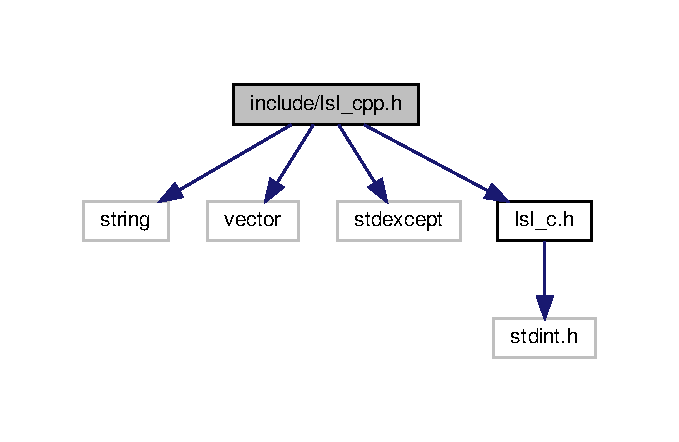
\includegraphics[width=326pt]{dd/d85/lsl__cpp_8h__incl}
\end{center}
\end{figure}
This graph shows which files directly or indirectly include this file\+:\nopagebreak
\begin{figure}[H]
\begin{center}
\leavevmode
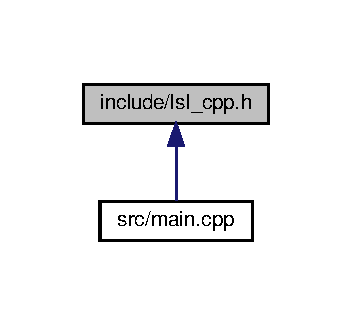
\includegraphics[width=169pt]{dd/d00/lsl__cpp_8h__dep__incl}
\end{center}
\end{figure}
\subsection*{Classes}
\begin{DoxyCompactItemize}
\item 
class \hyperlink{classlsl_1_1stream__info}{lsl\+::stream\+\_\+info}
\item 
class \hyperlink{classlsl_1_1stream__outlet}{lsl\+::stream\+\_\+outlet}
\item 
class \hyperlink{classlsl_1_1stream__inlet}{lsl\+::stream\+\_\+inlet}
\item 
class \hyperlink{classlsl_1_1xml__element}{lsl\+::xml\+\_\+element}
\item 
class \hyperlink{classlsl_1_1continuous__resolver}{lsl\+::continuous\+\_\+resolver}
\item 
class \hyperlink{classlsl_1_1lost__error}{lsl\+::lost\+\_\+error}
\begin{DoxyCompactList}\small\item\em Exception class that indicates that a stream inlet\textquotesingle{}s source has been irrecoverably lost. \end{DoxyCompactList}\item 
class \hyperlink{classlsl_1_1timeout__error}{lsl\+::timeout\+\_\+error}
\begin{DoxyCompactList}\small\item\em Exception class that indicates that an operation failed due to a timeout. \end{DoxyCompactList}\end{DoxyCompactItemize}
\subsection*{Namespaces}
\begin{DoxyCompactItemize}
\item 
 \hyperlink{namespacelsl}{lsl}
\end{DoxyCompactItemize}
\subsection*{Typedefs}
\begin{DoxyCompactItemize}
\item 
typedef struct lsl\+\_\+streaminfo\+\_\+struct\+\_\+ $\ast$ \hyperlink{namespacelsl_aa0a9ce9956061679949daa2e35aae2e8}{lsl\+::lsl\+\_\+streaminfo}
\item 
typedef struct lsl\+\_\+outlet\+\_\+struct\+\_\+ $\ast$ \hyperlink{namespacelsl_abcf512b0f66dacf86c10b165995fd50b}{lsl\+::lsl\+\_\+outlet}
\item 
typedef struct lsl\+\_\+inlet\+\_\+struct\+\_\+ $\ast$ \hyperlink{namespacelsl_a884a3363cfcba75d7ce8f00c1c4c54f1}{lsl\+::lsl\+\_\+inlet}
\item 
typedef struct lsl\+\_\+xml\+\_\+ptr\+\_\+struct\+\_\+ $\ast$ \hyperlink{namespacelsl_a5edc7a49a1a1be1634fe6dce3d59c59b}{lsl\+::lsl\+\_\+xml\+\_\+ptr}
\item 
typedef struct lsl\+\_\+continuous\+\_\+resolver\+\_\+ $\ast$ \hyperlink{namespacelsl_ab09ea0488f986f056322c3c866dc0a0f}{lsl\+::lsl\+\_\+continuous\+\_\+resolver}
\end{DoxyCompactItemize}
\subsection*{Enumerations}
\begin{DoxyCompactItemize}
\item 
enum \hyperlink{namespacelsl_af188e978739868560b53dbf0ddd58e66}{lsl\+::lsl\+\_\+channel\+\_\+format\+\_\+t} \{ \newline
\hyperlink{namespacelsl_af188e978739868560b53dbf0ddd58e66aa95674227416b8ac1738687b32238d2f}{lsl\+::cft\+\_\+float32} = 1, 
\hyperlink{namespacelsl_af188e978739868560b53dbf0ddd58e66a5774bc95ff1f184ac12aff46fb7b68bc}{lsl\+::cft\+\_\+double64} = 2, 
\hyperlink{namespacelsl_af188e978739868560b53dbf0ddd58e66a6c5dce46d2515d637a2d25fb6bec4c00}{lsl\+::cft\+\_\+string} = 3, 
\hyperlink{namespacelsl_af188e978739868560b53dbf0ddd58e66a0953ae3a0b24ddcf260e0d21efede185}{lsl\+::cft\+\_\+int32} = 4, 
\newline
\hyperlink{namespacelsl_af188e978739868560b53dbf0ddd58e66a6476b2e6f58fdcb5e4614724fb9ab47c}{lsl\+::cft\+\_\+int16} = 5, 
\hyperlink{namespacelsl_af188e978739868560b53dbf0ddd58e66afe29bb90886dc301279506a17dad1c64}{lsl\+::cft\+\_\+int8} = 6, 
\hyperlink{namespacelsl_af188e978739868560b53dbf0ddd58e66a1c41c8b332c529710af7b3669256e24d}{lsl\+::cft\+\_\+int64} = 7, 
\hyperlink{namespacelsl_af188e978739868560b53dbf0ddd58e66a86446aa37b10c9094f36113fd2ff91a8}{lsl\+::cft\+\_\+undefined} = 0
 \}
\item 
enum \hyperlink{namespacelsl_a71fa5faeecfdd863828bdcd4117e736b}{lsl\+::lsl\+\_\+processing\+\_\+options\+\_\+t} \{ \newline
\hyperlink{namespacelsl_a71fa5faeecfdd863828bdcd4117e736bab96deb7b18bc02826a6cfec6007bcea2}{lsl\+::proc\+\_\+none} = 0, 
\hyperlink{namespacelsl_a71fa5faeecfdd863828bdcd4117e736baec0e5bf31072a78138faa6601786fd59}{lsl\+::proc\+\_\+clocksync} = 1, 
\hyperlink{namespacelsl_a71fa5faeecfdd863828bdcd4117e736baa29c9fe911f4bd26adc8d3b2c0b63d7e}{lsl\+::proc\+\_\+dejitter} = 2, 
\hyperlink{namespacelsl_a71fa5faeecfdd863828bdcd4117e736ba88bf55224b0d66a340e1715667e39844}{lsl\+::proc\+\_\+monotonize} = 4, 
\newline
\hyperlink{namespacelsl_a71fa5faeecfdd863828bdcd4117e736ba67d7ca683f860c6c2768d428e5aa9997}{lsl\+::proc\+\_\+threadsafe} = 8, 
\hyperlink{namespacelsl_a71fa5faeecfdd863828bdcd4117e736ba969800e5a22f6a2e0972e41c5d5f1069}{lsl\+::proc\+\_\+\+A\+LL} = 1$\vert$2$\vert$4$\vert$8
 \}
\item 
enum \hyperlink{namespacelsl_a7e674c7665887951b952c463258451a9}{lsl\+::lsl\+\_\+error\+\_\+code\+\_\+t} \{ \newline
\hyperlink{namespacelsl_a7e674c7665887951b952c463258451a9a989effee9a9144bef995cb444fbde661}{lsl\+::lsl\+\_\+no\+\_\+error} = 0, 
\hyperlink{namespacelsl_a7e674c7665887951b952c463258451a9ac063592a9084fc6f2880de7172e78953}{lsl\+::lsl\+\_\+timeout\+\_\+error} = -\/1, 
\hyperlink{namespacelsl_a7e674c7665887951b952c463258451a9a348c8927eaa743c43d6efce38ec685c6}{lsl\+::lsl\+\_\+lost\+\_\+error} = -\/2, 
\hyperlink{namespacelsl_a7e674c7665887951b952c463258451a9af33e23dbe65f80c38e7d130903586001}{lsl\+::lsl\+\_\+argument\+\_\+error} = -\/3, 
\newline
\hyperlink{namespacelsl_a7e674c7665887951b952c463258451a9ae8db9e5ef7617a71bf95505c0e77fe75}{lsl\+::lsl\+\_\+internal\+\_\+error} = -\/4
 \}
\item 
enum \hyperlink{namespacelsl_a28d50dae6fd82eea8893ce3d63ccd46c}{lsl\+::channel\+\_\+format\+\_\+t} \{ \newline
\hyperlink{namespacelsl_a28d50dae6fd82eea8893ce3d63ccd46ca46efa3307b337f7de592753642584616}{lsl\+::cf\+\_\+float32} = 1, 
\hyperlink{namespacelsl_a28d50dae6fd82eea8893ce3d63ccd46cab11213c3d307faf6ef734633ac732eb7}{lsl\+::cf\+\_\+double64} = 2, 
\hyperlink{namespacelsl_a28d50dae6fd82eea8893ce3d63ccd46caedadbd6437a22628678edaf287c87048}{lsl\+::cf\+\_\+string} = 3, 
\hyperlink{namespacelsl_a28d50dae6fd82eea8893ce3d63ccd46ca526ce3ccb97e3bb75d913c60ad56c26d}{lsl\+::cf\+\_\+int32} = 4, 
\newline
\hyperlink{namespacelsl_a28d50dae6fd82eea8893ce3d63ccd46ca5c625662462c8a30454f6f7f0520e79c}{lsl\+::cf\+\_\+int16} = 5, 
\hyperlink{namespacelsl_a28d50dae6fd82eea8893ce3d63ccd46ca829ae156932f587fbbc70aed1d46e388}{lsl\+::cf\+\_\+int8} = 6, 
\hyperlink{namespacelsl_a28d50dae6fd82eea8893ce3d63ccd46ca6795e1df0db0b05744fd1fe9623567a0}{lsl\+::cf\+\_\+int64} = 7, 
\hyperlink{namespacelsl_a28d50dae6fd82eea8893ce3d63ccd46cadc8092d1092568f7d36d89fa7e813d76}{lsl\+::cf\+\_\+undefined} = 0
 \}
\item 
enum \hyperlink{namespacelsl_aaa1cffa7d29bb2756522bc2bb069e310}{lsl\+::processing\+\_\+options\+\_\+t} \{ \newline
\hyperlink{namespacelsl_aaa1cffa7d29bb2756522bc2bb069e310ac01170c28c82b28d721da1971e16424b}{lsl\+::post\+\_\+none} = 0, 
\hyperlink{namespacelsl_aaa1cffa7d29bb2756522bc2bb069e310accf7cbfa478e679b53255d46fd62f888}{lsl\+::post\+\_\+clocksync} = 1, 
\hyperlink{namespacelsl_aaa1cffa7d29bb2756522bc2bb069e310a83b67e37c1bbcfb4ee7479098386499f}{lsl\+::post\+\_\+dejitter} = 2, 
\hyperlink{namespacelsl_aaa1cffa7d29bb2756522bc2bb069e310af7cdac323760b9cb6587733a24f5aecb}{lsl\+::post\+\_\+monotonize} = 4, 
\newline
\hyperlink{namespacelsl_aaa1cffa7d29bb2756522bc2bb069e310a8ebef2c4c98e1a9246e9927e6b0b87c9}{lsl\+::post\+\_\+threadsafe} = 8, 
\hyperlink{namespacelsl_aaa1cffa7d29bb2756522bc2bb069e310a198f16659e71b850e4674ed31d10e914}{lsl\+::post\+\_\+\+A\+LL} = 1$\vert$2$\vert$4$\vert$8
 \}
\end{DoxyCompactItemize}
\subsection*{Functions}
\begin{DoxyCompactItemize}
\item 
\hyperlink{lsl__cpp_8h_aafd0ef1813e8be84a1420c4f1df64615}{L\+I\+B\+L\+S\+L\+\_\+\+C\+\_\+\+A\+PI} int32\+\_\+t \hyperlink{namespacelsl_a9695264d0e763474d352767702b38222}{lsl\+::lsl\+\_\+protocol\+\_\+version} ()
\item 
\hyperlink{lsl__cpp_8h_aafd0ef1813e8be84a1420c4f1df64615}{L\+I\+B\+L\+S\+L\+\_\+\+C\+\_\+\+A\+PI} int32\+\_\+t \hyperlink{namespacelsl_aa706e1332352902a9b531a88af671896}{lsl\+::lsl\+\_\+library\+\_\+version} ()
\item 
\hyperlink{lsl__cpp_8h_aafd0ef1813e8be84a1420c4f1df64615}{L\+I\+B\+L\+S\+L\+\_\+\+C\+\_\+\+A\+PI} const char $\ast$ \hyperlink{namespacelsl_a4e35f8426ffee9dbe7139dbe404e0442}{lsl\+::lsl\+\_\+library\+\_\+info} ()
\item 
\hyperlink{lsl__cpp_8h_aafd0ef1813e8be84a1420c4f1df64615}{L\+I\+B\+L\+S\+L\+\_\+\+C\+\_\+\+A\+PI} double \hyperlink{namespacelsl_a475274f88a060924c9bd1b38879ec63a}{lsl\+::lsl\+\_\+local\+\_\+clock} ()
\item 
\hyperlink{lsl__cpp_8h_aafd0ef1813e8be84a1420c4f1df64615}{L\+I\+B\+L\+S\+L\+\_\+\+C\+\_\+\+A\+PI} int32\+\_\+t \hyperlink{namespacelsl_a075ab08464c90d97b8f081d89ea889f2}{lsl\+::lsl\+\_\+resolve\+\_\+all} (\hyperlink{lsl__c_8h_a6fd635c662a9c80840b53bd7c202499c}{lsl\+\_\+streaminfo} $\ast$buffer, uint32\+\_\+t buffer\+\_\+elements, double wait\+\_\+time)
\item 
\hyperlink{lsl__cpp_8h_aafd0ef1813e8be84a1420c4f1df64615}{L\+I\+B\+L\+S\+L\+\_\+\+C\+\_\+\+A\+PI} int32\+\_\+t \hyperlink{namespacelsl_a66563e2290de3b056a5480ced8596ec7}{lsl\+::lsl\+\_\+resolve\+\_\+byprop} (\hyperlink{lsl__c_8h_a6fd635c662a9c80840b53bd7c202499c}{lsl\+\_\+streaminfo} $\ast$buffer, uint32\+\_\+t buffer\+\_\+elements, const char $\ast$prop, const char $\ast$value, int32\+\_\+t minimum, double timeout)
\item 
\hyperlink{lsl__cpp_8h_aafd0ef1813e8be84a1420c4f1df64615}{L\+I\+B\+L\+S\+L\+\_\+\+C\+\_\+\+A\+PI} int32\+\_\+t \hyperlink{namespacelsl_a11a5ef91d32961e0ad1d44dbef948399}{lsl\+::lsl\+\_\+resolve\+\_\+bypred} (\hyperlink{lsl__c_8h_a6fd635c662a9c80840b53bd7c202499c}{lsl\+\_\+streaminfo} $\ast$buffer, uint32\+\_\+t buffer\+\_\+elements, const char $\ast$pred, int32\+\_\+t minimum, double timeout)
\item 
\hyperlink{lsl__cpp_8h_aafd0ef1813e8be84a1420c4f1df64615}{L\+I\+B\+L\+S\+L\+\_\+\+C\+\_\+\+A\+PI} void \hyperlink{namespacelsl_ac517533eaabb224fd2f893e1f4274d82}{lsl\+::lsl\+\_\+destroy\+\_\+string} (char $\ast$s)
\item 
\hyperlink{lsl__cpp_8h_aafd0ef1813e8be84a1420c4f1df64615}{L\+I\+B\+L\+S\+L\+\_\+\+C\+\_\+\+A\+PI} \hyperlink{lsl__c_8h_a6fd635c662a9c80840b53bd7c202499c}{lsl\+\_\+streaminfo} \hyperlink{namespacelsl_abf20c6316cd58a713a674ef2213914d2}{lsl\+::lsl\+\_\+create\+\_\+streaminfo} (const char $\ast$name, const char $\ast$type, int32\+\_\+t channel\+\_\+count, double nominal\+\_\+srate, \hyperlink{lsl__c_8h_ad346feb32bddd136c3f7797e45047754}{lsl\+\_\+channel\+\_\+format\+\_\+t} channel\+\_\+format, const char $\ast$source\+\_\+id)
\item 
\hyperlink{lsl__cpp_8h_aafd0ef1813e8be84a1420c4f1df64615}{L\+I\+B\+L\+S\+L\+\_\+\+C\+\_\+\+A\+PI} void \hyperlink{namespacelsl_afc7ae71903a0c20763937739fa62df32}{lsl\+::lsl\+\_\+destroy\+\_\+streaminfo} (\hyperlink{lsl__c_8h_a6fd635c662a9c80840b53bd7c202499c}{lsl\+\_\+streaminfo} info)
\item 
\hyperlink{lsl__cpp_8h_aafd0ef1813e8be84a1420c4f1df64615}{L\+I\+B\+L\+S\+L\+\_\+\+C\+\_\+\+A\+PI} \hyperlink{lsl__c_8h_a6fd635c662a9c80840b53bd7c202499c}{lsl\+\_\+streaminfo} \hyperlink{namespacelsl_a354a91fa3a4c87cdf179443650425390}{lsl\+::lsl\+\_\+copy\+\_\+streaminfo} (\hyperlink{lsl__c_8h_a6fd635c662a9c80840b53bd7c202499c}{lsl\+\_\+streaminfo} info)
\item 
\hyperlink{lsl__cpp_8h_aafd0ef1813e8be84a1420c4f1df64615}{L\+I\+B\+L\+S\+L\+\_\+\+C\+\_\+\+A\+PI} const char $\ast$ \hyperlink{namespacelsl_ad356f55776a73d03998837c5c32fc95e}{lsl\+::lsl\+\_\+get\+\_\+name} (\hyperlink{lsl__c_8h_a6fd635c662a9c80840b53bd7c202499c}{lsl\+\_\+streaminfo} info)
\item 
\hyperlink{lsl__cpp_8h_aafd0ef1813e8be84a1420c4f1df64615}{L\+I\+B\+L\+S\+L\+\_\+\+C\+\_\+\+A\+PI} const char $\ast$ \hyperlink{namespacelsl_a417e01d26d64718513bc0ef2c58acf89}{lsl\+::lsl\+\_\+get\+\_\+type} (\hyperlink{lsl__c_8h_a6fd635c662a9c80840b53bd7c202499c}{lsl\+\_\+streaminfo} info)
\item 
\hyperlink{lsl__cpp_8h_aafd0ef1813e8be84a1420c4f1df64615}{L\+I\+B\+L\+S\+L\+\_\+\+C\+\_\+\+A\+PI} int32\+\_\+t \hyperlink{namespacelsl_a40acd87a21d3c91a524bd72012dc3328}{lsl\+::lsl\+\_\+get\+\_\+channel\+\_\+count} (\hyperlink{lsl__c_8h_a6fd635c662a9c80840b53bd7c202499c}{lsl\+\_\+streaminfo} info)
\item 
\hyperlink{lsl__cpp_8h_aafd0ef1813e8be84a1420c4f1df64615}{L\+I\+B\+L\+S\+L\+\_\+\+C\+\_\+\+A\+PI} double \hyperlink{namespacelsl_a17e4e6d432dc0b7280df4b5365c7da46}{lsl\+::lsl\+\_\+get\+\_\+nominal\+\_\+srate} (\hyperlink{lsl__c_8h_a6fd635c662a9c80840b53bd7c202499c}{lsl\+\_\+streaminfo} info)
\item 
\hyperlink{lsl__cpp_8h_aafd0ef1813e8be84a1420c4f1df64615}{L\+I\+B\+L\+S\+L\+\_\+\+C\+\_\+\+A\+PI} \hyperlink{lsl__c_8h_ad346feb32bddd136c3f7797e45047754}{lsl\+\_\+channel\+\_\+format\+\_\+t} \hyperlink{namespacelsl_a70c26257a8f3042084140a85a867a300}{lsl\+::lsl\+\_\+get\+\_\+channel\+\_\+format} (\hyperlink{lsl__c_8h_a6fd635c662a9c80840b53bd7c202499c}{lsl\+\_\+streaminfo} info)
\item 
\hyperlink{lsl__cpp_8h_aafd0ef1813e8be84a1420c4f1df64615}{L\+I\+B\+L\+S\+L\+\_\+\+C\+\_\+\+A\+PI} const char $\ast$ \hyperlink{namespacelsl_ad2987f3c32e0edae147498a8870a3215}{lsl\+::lsl\+\_\+get\+\_\+source\+\_\+id} (\hyperlink{lsl__c_8h_a6fd635c662a9c80840b53bd7c202499c}{lsl\+\_\+streaminfo} info)
\item 
\hyperlink{lsl__cpp_8h_aafd0ef1813e8be84a1420c4f1df64615}{L\+I\+B\+L\+S\+L\+\_\+\+C\+\_\+\+A\+PI} int32\+\_\+t \hyperlink{namespacelsl_ab889dd6f9a5fc6d6cd01a0b3dc153387}{lsl\+::lsl\+\_\+get\+\_\+version} (\hyperlink{lsl__c_8h_a6fd635c662a9c80840b53bd7c202499c}{lsl\+\_\+streaminfo} info)
\item 
\hyperlink{lsl__cpp_8h_aafd0ef1813e8be84a1420c4f1df64615}{L\+I\+B\+L\+S\+L\+\_\+\+C\+\_\+\+A\+PI} double \hyperlink{namespacelsl_aded8755dc0f65d8219449ef37ba7f6c5}{lsl\+::lsl\+\_\+get\+\_\+created\+\_\+at} (\hyperlink{lsl__c_8h_a6fd635c662a9c80840b53bd7c202499c}{lsl\+\_\+streaminfo} info)
\item 
\hyperlink{lsl__cpp_8h_aafd0ef1813e8be84a1420c4f1df64615}{L\+I\+B\+L\+S\+L\+\_\+\+C\+\_\+\+A\+PI} const char $\ast$ \hyperlink{namespacelsl_a6e18a9b1c544932e96179a44bb1f31ec}{lsl\+::lsl\+\_\+get\+\_\+uid} (\hyperlink{lsl__c_8h_a6fd635c662a9c80840b53bd7c202499c}{lsl\+\_\+streaminfo} info)
\item 
\hyperlink{lsl__cpp_8h_aafd0ef1813e8be84a1420c4f1df64615}{L\+I\+B\+L\+S\+L\+\_\+\+C\+\_\+\+A\+PI} const char $\ast$ \hyperlink{namespacelsl_ae28332bda70380cfd546fc158cd6f009}{lsl\+::lsl\+\_\+get\+\_\+session\+\_\+id} (\hyperlink{lsl__c_8h_a6fd635c662a9c80840b53bd7c202499c}{lsl\+\_\+streaminfo} info)
\item 
\hyperlink{lsl__cpp_8h_aafd0ef1813e8be84a1420c4f1df64615}{L\+I\+B\+L\+S\+L\+\_\+\+C\+\_\+\+A\+PI} const char $\ast$ \hyperlink{namespacelsl_ab74235be779da7e0cdcfd59b498bdf3f}{lsl\+::lsl\+\_\+get\+\_\+hostname} (\hyperlink{lsl__c_8h_a6fd635c662a9c80840b53bd7c202499c}{lsl\+\_\+streaminfo} info)
\item 
\hyperlink{lsl__cpp_8h_aafd0ef1813e8be84a1420c4f1df64615}{L\+I\+B\+L\+S\+L\+\_\+\+C\+\_\+\+A\+PI} \hyperlink{lsl__c_8h_ab174601268a7f0a9b60223510ba7d3b8}{lsl\+\_\+xml\+\_\+ptr} \hyperlink{namespacelsl_aeb428e46e46db8bd534e45ed8a76a120}{lsl\+::lsl\+\_\+get\+\_\+desc} (\hyperlink{lsl__c_8h_a6fd635c662a9c80840b53bd7c202499c}{lsl\+\_\+streaminfo} info)
\item 
\hyperlink{lsl__cpp_8h_aafd0ef1813e8be84a1420c4f1df64615}{L\+I\+B\+L\+S\+L\+\_\+\+C\+\_\+\+A\+PI} char $\ast$ \hyperlink{namespacelsl_ad1a9b14dccf565e5ecb79c093fe0fd39}{lsl\+::lsl\+\_\+get\+\_\+xml} (\hyperlink{lsl__c_8h_a6fd635c662a9c80840b53bd7c202499c}{lsl\+\_\+streaminfo} info)
\item 
\hyperlink{lsl__cpp_8h_aafd0ef1813e8be84a1420c4f1df64615}{L\+I\+B\+L\+S\+L\+\_\+\+C\+\_\+\+A\+PI} int32\+\_\+t \hyperlink{namespacelsl_aa11d6865aa57caf51f5d13c66a785b30}{lsl\+::lsl\+\_\+get\+\_\+channel\+\_\+bytes} (\hyperlink{lsl__c_8h_a6fd635c662a9c80840b53bd7c202499c}{lsl\+\_\+streaminfo} info)
\begin{DoxyCompactList}\small\item\em Number of bytes occupied by a channel (0 for string-\/typed channels). \end{DoxyCompactList}\item 
\hyperlink{lsl__cpp_8h_aafd0ef1813e8be84a1420c4f1df64615}{L\+I\+B\+L\+S\+L\+\_\+\+C\+\_\+\+A\+PI} int32\+\_\+t \hyperlink{namespacelsl_a26e8a9f4b8c7ee128362aadbc688dab0}{lsl\+::lsl\+\_\+get\+\_\+sample\+\_\+bytes} (\hyperlink{lsl__c_8h_a6fd635c662a9c80840b53bd7c202499c}{lsl\+\_\+streaminfo} info)
\begin{DoxyCompactList}\small\item\em Number of bytes occupied by a sample (0 for string-\/typed channels). \end{DoxyCompactList}\item 
\hyperlink{lsl__cpp_8h_aafd0ef1813e8be84a1420c4f1df64615}{L\+I\+B\+L\+S\+L\+\_\+\+C\+\_\+\+A\+PI} int \hyperlink{namespacelsl_a5c10ba1783b34bd0b3f048ac4cb5fe5e}{lsl\+::lsl\+\_\+stream\+\_\+info\+\_\+matches\+\_\+query} (\hyperlink{lsl__c_8h_a6fd635c662a9c80840b53bd7c202499c}{lsl\+\_\+streaminfo} info, const char $\ast$query)
\item 
\hyperlink{lsl__cpp_8h_aafd0ef1813e8be84a1420c4f1df64615}{L\+I\+B\+L\+S\+L\+\_\+\+C\+\_\+\+A\+PI} \hyperlink{lsl__c_8h_a6fd635c662a9c80840b53bd7c202499c}{lsl\+\_\+streaminfo} \hyperlink{namespacelsl_a2cf7fb16bf4029ca632fa5dab930de47}{lsl\+::lsl\+\_\+streaminfo\+\_\+from\+\_\+xml} (const char $\ast$xml)
\begin{DoxyCompactList}\small\item\em Create a streaminfo object from an X\+ML representation. \end{DoxyCompactList}\item 
\hyperlink{lsl__cpp_8h_aafd0ef1813e8be84a1420c4f1df64615}{L\+I\+B\+L\+S\+L\+\_\+\+C\+\_\+\+A\+PI} \hyperlink{lsl__c_8h_aef1212b6b2cd3e3747fd6e433c30e395}{lsl\+\_\+outlet} \hyperlink{namespacelsl_a4c92219e56eec896266a36ae58426d4b}{lsl\+::lsl\+\_\+create\+\_\+outlet} (\hyperlink{lsl__c_8h_a6fd635c662a9c80840b53bd7c202499c}{lsl\+\_\+streaminfo} info, int32\+\_\+t chunk\+\_\+size, int32\+\_\+t max\+\_\+buffered)
\item 
\hyperlink{lsl__cpp_8h_aafd0ef1813e8be84a1420c4f1df64615}{L\+I\+B\+L\+S\+L\+\_\+\+C\+\_\+\+A\+PI} void \hyperlink{namespacelsl_aa39980eac53711feece8bfc3b50d2b24}{lsl\+::lsl\+\_\+destroy\+\_\+outlet} (\hyperlink{lsl__c_8h_aef1212b6b2cd3e3747fd6e433c30e395}{lsl\+\_\+outlet} out)
\item 
\hyperlink{lsl__cpp_8h_aafd0ef1813e8be84a1420c4f1df64615}{L\+I\+B\+L\+S\+L\+\_\+\+C\+\_\+\+A\+PI} int32\+\_\+t \hyperlink{namespacelsl_a001aa3637915875c44c379c07c55fb3a}{lsl\+::lsl\+\_\+push\+\_\+sample\+\_\+f} (\hyperlink{lsl__c_8h_aef1212b6b2cd3e3747fd6e433c30e395}{lsl\+\_\+outlet} out, const float $\ast$data)
\item 
\hyperlink{lsl__cpp_8h_aafd0ef1813e8be84a1420c4f1df64615}{L\+I\+B\+L\+S\+L\+\_\+\+C\+\_\+\+A\+PI} int32\+\_\+t \hyperlink{namespacelsl_ade95641430ee28ac2bbcf888f572d34f}{lsl\+::lsl\+\_\+push\+\_\+sample\+\_\+ft} (\hyperlink{lsl__c_8h_aef1212b6b2cd3e3747fd6e433c30e395}{lsl\+\_\+outlet} out, const float $\ast$data, double timestamp)
\item 
\hyperlink{lsl__cpp_8h_aafd0ef1813e8be84a1420c4f1df64615}{L\+I\+B\+L\+S\+L\+\_\+\+C\+\_\+\+A\+PI} int32\+\_\+t \hyperlink{namespacelsl_a6434485fd96e3260939bfe6fea2b317e}{lsl\+::lsl\+\_\+push\+\_\+sample\+\_\+ftp} (\hyperlink{lsl__c_8h_aef1212b6b2cd3e3747fd6e433c30e395}{lsl\+\_\+outlet} out, const float $\ast$data, double timestamp, int32\+\_\+t pushthrough)
\item 
\hyperlink{lsl__cpp_8h_aafd0ef1813e8be84a1420c4f1df64615}{L\+I\+B\+L\+S\+L\+\_\+\+C\+\_\+\+A\+PI} int32\+\_\+t \hyperlink{namespacelsl_ac7d63bbdbdd3b0ec26d49b22b5858d8e}{lsl\+::lsl\+\_\+push\+\_\+sample\+\_\+d} (\hyperlink{lsl__c_8h_aef1212b6b2cd3e3747fd6e433c30e395}{lsl\+\_\+outlet} out, const double $\ast$data)
\item 
\hyperlink{lsl__cpp_8h_aafd0ef1813e8be84a1420c4f1df64615}{L\+I\+B\+L\+S\+L\+\_\+\+C\+\_\+\+A\+PI} int32\+\_\+t \hyperlink{namespacelsl_a6877d8a4ebbe802a123a09505a106f3f}{lsl\+::lsl\+\_\+push\+\_\+sample\+\_\+dt} (\hyperlink{lsl__c_8h_aef1212b6b2cd3e3747fd6e433c30e395}{lsl\+\_\+outlet} out, const double $\ast$data, double timestamp)
\item 
\hyperlink{lsl__cpp_8h_aafd0ef1813e8be84a1420c4f1df64615}{L\+I\+B\+L\+S\+L\+\_\+\+C\+\_\+\+A\+PI} int32\+\_\+t \hyperlink{namespacelsl_aa6064248da7a261b46185ec9ffd12ba3}{lsl\+::lsl\+\_\+push\+\_\+sample\+\_\+dtp} (\hyperlink{lsl__c_8h_aef1212b6b2cd3e3747fd6e433c30e395}{lsl\+\_\+outlet} out, const double $\ast$data, double timestamp, int32\+\_\+t pushthrough)
\item 
\hyperlink{lsl__cpp_8h_aafd0ef1813e8be84a1420c4f1df64615}{L\+I\+B\+L\+S\+L\+\_\+\+C\+\_\+\+A\+PI} int32\+\_\+t \hyperlink{namespacelsl_a44dd3e59bb5d7e95b9ffa60032207457}{lsl\+::lsl\+\_\+push\+\_\+sample\+\_\+l} (\hyperlink{lsl__c_8h_aef1212b6b2cd3e3747fd6e433c30e395}{lsl\+\_\+outlet} out, const long $\ast$data)
\item 
\hyperlink{lsl__cpp_8h_aafd0ef1813e8be84a1420c4f1df64615}{L\+I\+B\+L\+S\+L\+\_\+\+C\+\_\+\+A\+PI} int32\+\_\+t \hyperlink{namespacelsl_ad257a8fe8aee5d302292dd40d93fe335}{lsl\+::lsl\+\_\+push\+\_\+sample\+\_\+lt} (\hyperlink{lsl__c_8h_aef1212b6b2cd3e3747fd6e433c30e395}{lsl\+\_\+outlet} out, const long $\ast$data, double timestamp)
\item 
\hyperlink{lsl__cpp_8h_aafd0ef1813e8be84a1420c4f1df64615}{L\+I\+B\+L\+S\+L\+\_\+\+C\+\_\+\+A\+PI} int32\+\_\+t \hyperlink{namespacelsl_a4839e55343dd8c3aea6c8e2a65d706ed}{lsl\+::lsl\+\_\+push\+\_\+sample\+\_\+ltp} (\hyperlink{lsl__c_8h_aef1212b6b2cd3e3747fd6e433c30e395}{lsl\+\_\+outlet} out, const long $\ast$data, double timestamp, int32\+\_\+t pushthrough)
\item 
\hyperlink{lsl__cpp_8h_aafd0ef1813e8be84a1420c4f1df64615}{L\+I\+B\+L\+S\+L\+\_\+\+C\+\_\+\+A\+PI} int32\+\_\+t \hyperlink{namespacelsl_a5e6e682a09b4c90732e4fc631d643384}{lsl\+::lsl\+\_\+push\+\_\+sample\+\_\+i} (\hyperlink{lsl__c_8h_aef1212b6b2cd3e3747fd6e433c30e395}{lsl\+\_\+outlet} out, const int32\+\_\+t $\ast$data)
\item 
\hyperlink{lsl__cpp_8h_aafd0ef1813e8be84a1420c4f1df64615}{L\+I\+B\+L\+S\+L\+\_\+\+C\+\_\+\+A\+PI} int32\+\_\+t \hyperlink{namespacelsl_a87f61ecb0058ef8cd14a84693770b51d}{lsl\+::lsl\+\_\+push\+\_\+sample\+\_\+it} (\hyperlink{lsl__c_8h_aef1212b6b2cd3e3747fd6e433c30e395}{lsl\+\_\+outlet} out, const int32\+\_\+t $\ast$data, double timestamp)
\item 
\hyperlink{lsl__cpp_8h_aafd0ef1813e8be84a1420c4f1df64615}{L\+I\+B\+L\+S\+L\+\_\+\+C\+\_\+\+A\+PI} int32\+\_\+t \hyperlink{namespacelsl_aa0f3b0ccc233ebed00178e189c4678af}{lsl\+::lsl\+\_\+push\+\_\+sample\+\_\+itp} (\hyperlink{lsl__c_8h_aef1212b6b2cd3e3747fd6e433c30e395}{lsl\+\_\+outlet} out, const int32\+\_\+t $\ast$data, double timestamp, int32\+\_\+t pushthrough)
\item 
\hyperlink{lsl__cpp_8h_aafd0ef1813e8be84a1420c4f1df64615}{L\+I\+B\+L\+S\+L\+\_\+\+C\+\_\+\+A\+PI} int32\+\_\+t \hyperlink{namespacelsl_a8d80592d7fd643d64533ef83f6808743}{lsl\+::lsl\+\_\+push\+\_\+sample\+\_\+s} (\hyperlink{lsl__c_8h_aef1212b6b2cd3e3747fd6e433c30e395}{lsl\+\_\+outlet} out, const int16\+\_\+t $\ast$data)
\item 
\hyperlink{lsl__cpp_8h_aafd0ef1813e8be84a1420c4f1df64615}{L\+I\+B\+L\+S\+L\+\_\+\+C\+\_\+\+A\+PI} int32\+\_\+t \hyperlink{namespacelsl_a9a22e090bfa2e61ec19d70dc9bb5908d}{lsl\+::lsl\+\_\+push\+\_\+sample\+\_\+st} (\hyperlink{lsl__c_8h_aef1212b6b2cd3e3747fd6e433c30e395}{lsl\+\_\+outlet} out, const int16\+\_\+t $\ast$data, double timestamp)
\item 
\hyperlink{lsl__cpp_8h_aafd0ef1813e8be84a1420c4f1df64615}{L\+I\+B\+L\+S\+L\+\_\+\+C\+\_\+\+A\+PI} int32\+\_\+t \hyperlink{namespacelsl_a916ebe3afa6e7b83d670211c7320df51}{lsl\+::lsl\+\_\+push\+\_\+sample\+\_\+stp} (\hyperlink{lsl__c_8h_aef1212b6b2cd3e3747fd6e433c30e395}{lsl\+\_\+outlet} out, const int16\+\_\+t $\ast$data, double timestamp, int32\+\_\+t pushthrough)
\item 
\hyperlink{lsl__cpp_8h_aafd0ef1813e8be84a1420c4f1df64615}{L\+I\+B\+L\+S\+L\+\_\+\+C\+\_\+\+A\+PI} int32\+\_\+t \hyperlink{namespacelsl_aff896f8925d3453857deabc1f9cfd24a}{lsl\+::lsl\+\_\+push\+\_\+sample\+\_\+c} (\hyperlink{lsl__c_8h_aef1212b6b2cd3e3747fd6e433c30e395}{lsl\+\_\+outlet} out, const char $\ast$data)
\item 
\hyperlink{lsl__cpp_8h_aafd0ef1813e8be84a1420c4f1df64615}{L\+I\+B\+L\+S\+L\+\_\+\+C\+\_\+\+A\+PI} int32\+\_\+t \hyperlink{namespacelsl_a321429ed29e2b8b944f7724361628ba9}{lsl\+::lsl\+\_\+push\+\_\+sample\+\_\+ct} (\hyperlink{lsl__c_8h_aef1212b6b2cd3e3747fd6e433c30e395}{lsl\+\_\+outlet} out, const char $\ast$data, double timestamp)
\item 
\hyperlink{lsl__cpp_8h_aafd0ef1813e8be84a1420c4f1df64615}{L\+I\+B\+L\+S\+L\+\_\+\+C\+\_\+\+A\+PI} int32\+\_\+t \hyperlink{namespacelsl_a7127acf0d2106d5ae673489510845f58}{lsl\+::lsl\+\_\+push\+\_\+sample\+\_\+ctp} (\hyperlink{lsl__c_8h_aef1212b6b2cd3e3747fd6e433c30e395}{lsl\+\_\+outlet} out, const char $\ast$data, double timestamp, int32\+\_\+t pushthrough)
\item 
\hyperlink{lsl__cpp_8h_aafd0ef1813e8be84a1420c4f1df64615}{L\+I\+B\+L\+S\+L\+\_\+\+C\+\_\+\+A\+PI} int32\+\_\+t \hyperlink{namespacelsl_a3da2b3303768776977e0d621e2990c0e}{lsl\+::lsl\+\_\+push\+\_\+sample\+\_\+str} (\hyperlink{lsl__c_8h_aef1212b6b2cd3e3747fd6e433c30e395}{lsl\+\_\+outlet} out, const char $\ast$$\ast$data)
\item 
\hyperlink{lsl__cpp_8h_aafd0ef1813e8be84a1420c4f1df64615}{L\+I\+B\+L\+S\+L\+\_\+\+C\+\_\+\+A\+PI} int32\+\_\+t \hyperlink{namespacelsl_a634f8191b28e9cb9b6edcf01aaead377}{lsl\+::lsl\+\_\+push\+\_\+sample\+\_\+strt} (\hyperlink{lsl__c_8h_aef1212b6b2cd3e3747fd6e433c30e395}{lsl\+\_\+outlet} out, const char $\ast$$\ast$data, double timestamp)
\item 
\hyperlink{lsl__cpp_8h_aafd0ef1813e8be84a1420c4f1df64615}{L\+I\+B\+L\+S\+L\+\_\+\+C\+\_\+\+A\+PI} int32\+\_\+t \hyperlink{namespacelsl_aeb9537e1d060020c99c47371b07bcb24}{lsl\+::lsl\+\_\+push\+\_\+sample\+\_\+strtp} (\hyperlink{lsl__c_8h_aef1212b6b2cd3e3747fd6e433c30e395}{lsl\+\_\+outlet} out, const char $\ast$$\ast$data, double timestamp, int32\+\_\+t pushthrough)
\item 
\hyperlink{lsl__cpp_8h_aafd0ef1813e8be84a1420c4f1df64615}{L\+I\+B\+L\+S\+L\+\_\+\+C\+\_\+\+A\+PI} int32\+\_\+t \hyperlink{namespacelsl_a77dbefbfa9fc565f9ead1db3574ef001}{lsl\+::lsl\+\_\+push\+\_\+sample\+\_\+buf} (\hyperlink{lsl__c_8h_aef1212b6b2cd3e3747fd6e433c30e395}{lsl\+\_\+outlet} out, const char $\ast$$\ast$data, const uint32\+\_\+t $\ast$lengths)
\item 
\hyperlink{lsl__cpp_8h_aafd0ef1813e8be84a1420c4f1df64615}{L\+I\+B\+L\+S\+L\+\_\+\+C\+\_\+\+A\+PI} int32\+\_\+t \hyperlink{namespacelsl_ace903fc8ac868a1afedf98090f5c5b4c}{lsl\+::lsl\+\_\+push\+\_\+sample\+\_\+buft} (\hyperlink{lsl__c_8h_aef1212b6b2cd3e3747fd6e433c30e395}{lsl\+\_\+outlet} out, const char $\ast$$\ast$data, const uint32\+\_\+t $\ast$lengths, double timestamp)
\item 
\hyperlink{lsl__cpp_8h_aafd0ef1813e8be84a1420c4f1df64615}{L\+I\+B\+L\+S\+L\+\_\+\+C\+\_\+\+A\+PI} int32\+\_\+t \hyperlink{namespacelsl_a62d7f7be3db90336d61e89633c4b1a5e}{lsl\+::lsl\+\_\+push\+\_\+sample\+\_\+buftp} (\hyperlink{lsl__c_8h_aef1212b6b2cd3e3747fd6e433c30e395}{lsl\+\_\+outlet} out, const char $\ast$$\ast$data, const uint32\+\_\+t $\ast$lengths, double timestamp, int32\+\_\+t pushthrough)
\item 
\hyperlink{lsl__cpp_8h_aafd0ef1813e8be84a1420c4f1df64615}{L\+I\+B\+L\+S\+L\+\_\+\+C\+\_\+\+A\+PI} int32\+\_\+t \hyperlink{namespacelsl_a25ee57785d5ab7143605ee9f59c1a0cf}{lsl\+::lsl\+\_\+push\+\_\+sample\+\_\+v} (\hyperlink{lsl__c_8h_aef1212b6b2cd3e3747fd6e433c30e395}{lsl\+\_\+outlet} out, const void $\ast$data)
\item 
\hyperlink{lsl__cpp_8h_aafd0ef1813e8be84a1420c4f1df64615}{L\+I\+B\+L\+S\+L\+\_\+\+C\+\_\+\+A\+PI} int32\+\_\+t \hyperlink{namespacelsl_a8032f4283b186f0f8b8e657f6642e062}{lsl\+::lsl\+\_\+push\+\_\+sample\+\_\+vt} (\hyperlink{lsl__c_8h_aef1212b6b2cd3e3747fd6e433c30e395}{lsl\+\_\+outlet} out, const void $\ast$data, double timestamp)
\item 
\hyperlink{lsl__cpp_8h_aafd0ef1813e8be84a1420c4f1df64615}{L\+I\+B\+L\+S\+L\+\_\+\+C\+\_\+\+A\+PI} int32\+\_\+t \hyperlink{namespacelsl_a750c5759d30e4e0a47223c7048bfa4ca}{lsl\+::lsl\+\_\+push\+\_\+sample\+\_\+vtp} (\hyperlink{lsl__c_8h_aef1212b6b2cd3e3747fd6e433c30e395}{lsl\+\_\+outlet} out, const void $\ast$data, double timestamp, int32\+\_\+t pushthrough)
\item 
\hyperlink{lsl__cpp_8h_aafd0ef1813e8be84a1420c4f1df64615}{L\+I\+B\+L\+S\+L\+\_\+\+C\+\_\+\+A\+PI} int32\+\_\+t \hyperlink{namespacelsl_abaf77814f92eec3728670d14195b460b}{lsl\+::lsl\+\_\+push\+\_\+chunk\+\_\+f} (\hyperlink{lsl__c_8h_aef1212b6b2cd3e3747fd6e433c30e395}{lsl\+\_\+outlet} out, const float $\ast$data, unsigned long data\+\_\+elements)
\item 
\hyperlink{lsl__cpp_8h_aafd0ef1813e8be84a1420c4f1df64615}{L\+I\+B\+L\+S\+L\+\_\+\+C\+\_\+\+A\+PI} int32\+\_\+t \hyperlink{namespacelsl_a115ed5e462c162787436cd9800dbcb7e}{lsl\+::lsl\+\_\+push\+\_\+chunk\+\_\+ft} (\hyperlink{lsl__c_8h_aef1212b6b2cd3e3747fd6e433c30e395}{lsl\+\_\+outlet} out, const float $\ast$data, unsigned long data\+\_\+elements, double timestamp)
\item 
\hyperlink{lsl__cpp_8h_aafd0ef1813e8be84a1420c4f1df64615}{L\+I\+B\+L\+S\+L\+\_\+\+C\+\_\+\+A\+PI} int32\+\_\+t \hyperlink{namespacelsl_adf8f3e407c2b25a0e68aaf4e27df742d}{lsl\+::lsl\+\_\+push\+\_\+chunk\+\_\+ftp} (\hyperlink{lsl__c_8h_aef1212b6b2cd3e3747fd6e433c30e395}{lsl\+\_\+outlet} out, const float $\ast$data, unsigned long data\+\_\+elements, double timestamp, int32\+\_\+t pushthrough)
\item 
\hyperlink{lsl__cpp_8h_aafd0ef1813e8be84a1420c4f1df64615}{L\+I\+B\+L\+S\+L\+\_\+\+C\+\_\+\+A\+PI} int32\+\_\+t \hyperlink{namespacelsl_aee7313f1b6a8c88e7bdfc5f133986aaa}{lsl\+::lsl\+\_\+push\+\_\+chunk\+\_\+ftn} (\hyperlink{lsl__c_8h_aef1212b6b2cd3e3747fd6e433c30e395}{lsl\+\_\+outlet} out, const float $\ast$data, unsigned long data\+\_\+elements, const double $\ast$timestamps)
\item 
\hyperlink{lsl__cpp_8h_aafd0ef1813e8be84a1420c4f1df64615}{L\+I\+B\+L\+S\+L\+\_\+\+C\+\_\+\+A\+PI} int32\+\_\+t \hyperlink{namespacelsl_a5bb763124a2b2e74423b5c382a600b30}{lsl\+::lsl\+\_\+push\+\_\+chunk\+\_\+ftnp} (\hyperlink{lsl__c_8h_aef1212b6b2cd3e3747fd6e433c30e395}{lsl\+\_\+outlet} out, const float $\ast$data, unsigned long data\+\_\+elements, const double $\ast$timestamps, int32\+\_\+t pushthrough)
\item 
\hyperlink{lsl__cpp_8h_aafd0ef1813e8be84a1420c4f1df64615}{L\+I\+B\+L\+S\+L\+\_\+\+C\+\_\+\+A\+PI} int32\+\_\+t \hyperlink{namespacelsl_aba0e49750a9d56a0058b4287652043b1}{lsl\+::lsl\+\_\+push\+\_\+chunk\+\_\+d} (\hyperlink{lsl__c_8h_aef1212b6b2cd3e3747fd6e433c30e395}{lsl\+\_\+outlet} out, const double $\ast$data, unsigned long data\+\_\+elements)
\item 
\hyperlink{lsl__cpp_8h_aafd0ef1813e8be84a1420c4f1df64615}{L\+I\+B\+L\+S\+L\+\_\+\+C\+\_\+\+A\+PI} int32\+\_\+t \hyperlink{namespacelsl_ae0c9d5ce50a5e9c7cd612063b82c7e6b}{lsl\+::lsl\+\_\+push\+\_\+chunk\+\_\+dt} (\hyperlink{lsl__c_8h_aef1212b6b2cd3e3747fd6e433c30e395}{lsl\+\_\+outlet} out, const double $\ast$data, unsigned long data\+\_\+elements, double timestamp)
\item 
\hyperlink{lsl__cpp_8h_aafd0ef1813e8be84a1420c4f1df64615}{L\+I\+B\+L\+S\+L\+\_\+\+C\+\_\+\+A\+PI} int32\+\_\+t \hyperlink{namespacelsl_afdd8325060d14312cb340bc2edcac10a}{lsl\+::lsl\+\_\+push\+\_\+chunk\+\_\+dtp} (\hyperlink{lsl__c_8h_aef1212b6b2cd3e3747fd6e433c30e395}{lsl\+\_\+outlet} out, const double $\ast$data, unsigned long data\+\_\+elements, double timestamp, int32\+\_\+t pushthrough)
\item 
\hyperlink{lsl__cpp_8h_aafd0ef1813e8be84a1420c4f1df64615}{L\+I\+B\+L\+S\+L\+\_\+\+C\+\_\+\+A\+PI} int32\+\_\+t \hyperlink{namespacelsl_ae0a8ffad75240ca3d702944ebf7d7d53}{lsl\+::lsl\+\_\+push\+\_\+chunk\+\_\+dtn} (\hyperlink{lsl__c_8h_aef1212b6b2cd3e3747fd6e433c30e395}{lsl\+\_\+outlet} out, const double $\ast$data, unsigned long data\+\_\+elements, const double $\ast$timestamps)
\item 
\hyperlink{lsl__cpp_8h_aafd0ef1813e8be84a1420c4f1df64615}{L\+I\+B\+L\+S\+L\+\_\+\+C\+\_\+\+A\+PI} int32\+\_\+t \hyperlink{namespacelsl_a8a0e5cfc6b88e4dae3d4abd97ac47c38}{lsl\+::lsl\+\_\+push\+\_\+chunk\+\_\+dtnp} (\hyperlink{lsl__c_8h_aef1212b6b2cd3e3747fd6e433c30e395}{lsl\+\_\+outlet} out, const double $\ast$data, unsigned long data\+\_\+elements, const double $\ast$timestamps, int32\+\_\+t pushthrough)
\item 
\hyperlink{lsl__cpp_8h_aafd0ef1813e8be84a1420c4f1df64615}{L\+I\+B\+L\+S\+L\+\_\+\+C\+\_\+\+A\+PI} int \hyperlink{namespacelsl_a68403934d1fdace37348c95f54367bc2}{lsl\+::lsl\+\_\+push\+\_\+chunk\+\_\+l} (\hyperlink{lsl__c_8h_aef1212b6b2cd3e3747fd6e433c30e395}{lsl\+\_\+outlet} out, const long $\ast$data, unsigned long data\+\_\+elements)
\item 
\hyperlink{lsl__cpp_8h_aafd0ef1813e8be84a1420c4f1df64615}{L\+I\+B\+L\+S\+L\+\_\+\+C\+\_\+\+A\+PI} int \hyperlink{namespacelsl_a55622b4fc53149f986414f7642baf00a}{lsl\+::lsl\+\_\+push\+\_\+chunk\+\_\+lt} (\hyperlink{lsl__c_8h_aef1212b6b2cd3e3747fd6e433c30e395}{lsl\+\_\+outlet} out, const long $\ast$data, unsigned long data\+\_\+elements, double timestamp)
\item 
\hyperlink{lsl__cpp_8h_aafd0ef1813e8be84a1420c4f1df64615}{L\+I\+B\+L\+S\+L\+\_\+\+C\+\_\+\+A\+PI} int \hyperlink{namespacelsl_a1a6be2ac3bc8a1df1f4c08d0b3a79445}{lsl\+::lsl\+\_\+push\+\_\+chunk\+\_\+ltp} (\hyperlink{lsl__c_8h_aef1212b6b2cd3e3747fd6e433c30e395}{lsl\+\_\+outlet} out, const long $\ast$data, unsigned long data\+\_\+elements, double timestamp, int pushthrough)
\item 
\hyperlink{lsl__cpp_8h_aafd0ef1813e8be84a1420c4f1df64615}{L\+I\+B\+L\+S\+L\+\_\+\+C\+\_\+\+A\+PI} int \hyperlink{namespacelsl_a93cfea6f1ecc01606e6e4f37bba7103f}{lsl\+::lsl\+\_\+push\+\_\+chunk\+\_\+ltn} (\hyperlink{lsl__c_8h_aef1212b6b2cd3e3747fd6e433c30e395}{lsl\+\_\+outlet} out, const long $\ast$data, unsigned long data\+\_\+elements, const double $\ast$timestamps)
\item 
\hyperlink{lsl__cpp_8h_aafd0ef1813e8be84a1420c4f1df64615}{L\+I\+B\+L\+S\+L\+\_\+\+C\+\_\+\+A\+PI} int \hyperlink{namespacelsl_aa172a29d0976aee8d41306d7b8b53231}{lsl\+::lsl\+\_\+push\+\_\+chunk\+\_\+ltnp} (\hyperlink{lsl__c_8h_aef1212b6b2cd3e3747fd6e433c30e395}{lsl\+\_\+outlet} out, const long $\ast$data, unsigned long data\+\_\+elements, const double $\ast$timestamps, int pushthrough)
\item 
\hyperlink{lsl__cpp_8h_aafd0ef1813e8be84a1420c4f1df64615}{L\+I\+B\+L\+S\+L\+\_\+\+C\+\_\+\+A\+PI} int32\+\_\+t \hyperlink{namespacelsl_a096b23637c04d20bcaea1a92bc438845}{lsl\+::lsl\+\_\+push\+\_\+chunk\+\_\+i} (\hyperlink{lsl__c_8h_aef1212b6b2cd3e3747fd6e433c30e395}{lsl\+\_\+outlet} out, const int32\+\_\+t $\ast$data, unsigned long data\+\_\+elements)
\item 
\hyperlink{lsl__cpp_8h_aafd0ef1813e8be84a1420c4f1df64615}{L\+I\+B\+L\+S\+L\+\_\+\+C\+\_\+\+A\+PI} int32\+\_\+t \hyperlink{namespacelsl_aede257c8d3911fbc26329bd4af8bcc9a}{lsl\+::lsl\+\_\+push\+\_\+chunk\+\_\+it} (\hyperlink{lsl__c_8h_aef1212b6b2cd3e3747fd6e433c30e395}{lsl\+\_\+outlet} out, const int32\+\_\+t $\ast$data, unsigned long data\+\_\+elements, double timestamp)
\item 
\hyperlink{lsl__cpp_8h_aafd0ef1813e8be84a1420c4f1df64615}{L\+I\+B\+L\+S\+L\+\_\+\+C\+\_\+\+A\+PI} int32\+\_\+t \hyperlink{namespacelsl_a38439e357a8d6c984ffcfd9e22596ec1}{lsl\+::lsl\+\_\+push\+\_\+chunk\+\_\+itp} (\hyperlink{lsl__c_8h_aef1212b6b2cd3e3747fd6e433c30e395}{lsl\+\_\+outlet} out, const int32\+\_\+t $\ast$data, unsigned long data\+\_\+elements, double timestamp, int32\+\_\+t pushthrough)
\item 
\hyperlink{lsl__cpp_8h_aafd0ef1813e8be84a1420c4f1df64615}{L\+I\+B\+L\+S\+L\+\_\+\+C\+\_\+\+A\+PI} int32\+\_\+t \hyperlink{namespacelsl_a0ea52f33684ceab15ad7244636291ddd}{lsl\+::lsl\+\_\+push\+\_\+chunk\+\_\+itn} (\hyperlink{lsl__c_8h_aef1212b6b2cd3e3747fd6e433c30e395}{lsl\+\_\+outlet} out, const int32\+\_\+t $\ast$data, unsigned long data\+\_\+elements, const double $\ast$timestamps)
\item 
\hyperlink{lsl__cpp_8h_aafd0ef1813e8be84a1420c4f1df64615}{L\+I\+B\+L\+S\+L\+\_\+\+C\+\_\+\+A\+PI} int32\+\_\+t \hyperlink{namespacelsl_a9102a7929e172f9a42e51211139d691f}{lsl\+::lsl\+\_\+push\+\_\+chunk\+\_\+itnp} (\hyperlink{lsl__c_8h_aef1212b6b2cd3e3747fd6e433c30e395}{lsl\+\_\+outlet} out, const int32\+\_\+t $\ast$data, unsigned long data\+\_\+elements, const double $\ast$timestamps, int32\+\_\+t pushthrough)
\item 
\hyperlink{lsl__cpp_8h_aafd0ef1813e8be84a1420c4f1df64615}{L\+I\+B\+L\+S\+L\+\_\+\+C\+\_\+\+A\+PI} int32\+\_\+t \hyperlink{namespacelsl_ac2e4e87bd196fe5469934eaf87ecdaa2}{lsl\+::lsl\+\_\+push\+\_\+chunk\+\_\+s} (\hyperlink{lsl__c_8h_aef1212b6b2cd3e3747fd6e433c30e395}{lsl\+\_\+outlet} out, const int16\+\_\+t $\ast$data, unsigned long data\+\_\+elements)
\item 
\hyperlink{lsl__cpp_8h_aafd0ef1813e8be84a1420c4f1df64615}{L\+I\+B\+L\+S\+L\+\_\+\+C\+\_\+\+A\+PI} int32\+\_\+t \hyperlink{namespacelsl_a6d02c87538ca2e49831fefc79a4ef751}{lsl\+::lsl\+\_\+push\+\_\+chunk\+\_\+st} (\hyperlink{lsl__c_8h_aef1212b6b2cd3e3747fd6e433c30e395}{lsl\+\_\+outlet} out, const int16\+\_\+t $\ast$data, unsigned long data\+\_\+elements, double timestamp)
\item 
\hyperlink{lsl__cpp_8h_aafd0ef1813e8be84a1420c4f1df64615}{L\+I\+B\+L\+S\+L\+\_\+\+C\+\_\+\+A\+PI} int32\+\_\+t \hyperlink{namespacelsl_a8de67854b1d0c9de42e3e69997f68d0c}{lsl\+::lsl\+\_\+push\+\_\+chunk\+\_\+stp} (\hyperlink{lsl__c_8h_aef1212b6b2cd3e3747fd6e433c30e395}{lsl\+\_\+outlet} out, const int16\+\_\+t $\ast$data, unsigned long data\+\_\+elements, double timestamp, int32\+\_\+t pushthrough)
\item 
\hyperlink{lsl__cpp_8h_aafd0ef1813e8be84a1420c4f1df64615}{L\+I\+B\+L\+S\+L\+\_\+\+C\+\_\+\+A\+PI} int32\+\_\+t \hyperlink{namespacelsl_a66784045ca9dec23b491f56474009de4}{lsl\+::lsl\+\_\+push\+\_\+chunk\+\_\+stn} (\hyperlink{lsl__c_8h_aef1212b6b2cd3e3747fd6e433c30e395}{lsl\+\_\+outlet} out, const int16\+\_\+t $\ast$data, unsigned long data\+\_\+elements, const double $\ast$timestamps)
\item 
\hyperlink{lsl__cpp_8h_aafd0ef1813e8be84a1420c4f1df64615}{L\+I\+B\+L\+S\+L\+\_\+\+C\+\_\+\+A\+PI} int32\+\_\+t \hyperlink{namespacelsl_aee4448b6c1239e14f9212700c828ca5b}{lsl\+::lsl\+\_\+push\+\_\+chunk\+\_\+stnp} (\hyperlink{lsl__c_8h_aef1212b6b2cd3e3747fd6e433c30e395}{lsl\+\_\+outlet} out, const int16\+\_\+t $\ast$data, unsigned long data\+\_\+elements, const double $\ast$timestamps, int32\+\_\+t pushthrough)
\item 
\hyperlink{lsl__cpp_8h_aafd0ef1813e8be84a1420c4f1df64615}{L\+I\+B\+L\+S\+L\+\_\+\+C\+\_\+\+A\+PI} int32\+\_\+t \hyperlink{namespacelsl_a3dd3622f5a0fcdedbc7bf4223a08ba01}{lsl\+::lsl\+\_\+push\+\_\+chunk\+\_\+c} (\hyperlink{lsl__c_8h_aef1212b6b2cd3e3747fd6e433c30e395}{lsl\+\_\+outlet} out, const char $\ast$data, unsigned long data\+\_\+elements)
\item 
\hyperlink{lsl__cpp_8h_aafd0ef1813e8be84a1420c4f1df64615}{L\+I\+B\+L\+S\+L\+\_\+\+C\+\_\+\+A\+PI} int32\+\_\+t \hyperlink{namespacelsl_a9bad246099db9f07ccc795d14709eed7}{lsl\+::lsl\+\_\+push\+\_\+chunk\+\_\+ct} (\hyperlink{lsl__c_8h_aef1212b6b2cd3e3747fd6e433c30e395}{lsl\+\_\+outlet} out, const char $\ast$data, unsigned long data\+\_\+elements, double timestamp)
\item 
\hyperlink{lsl__cpp_8h_aafd0ef1813e8be84a1420c4f1df64615}{L\+I\+B\+L\+S\+L\+\_\+\+C\+\_\+\+A\+PI} int32\+\_\+t \hyperlink{namespacelsl_ad8287dab0124b1f1d8a682e914116550}{lsl\+::lsl\+\_\+push\+\_\+chunk\+\_\+ctp} (\hyperlink{lsl__c_8h_aef1212b6b2cd3e3747fd6e433c30e395}{lsl\+\_\+outlet} out, const char $\ast$data, unsigned long data\+\_\+elements, double timestamp, int32\+\_\+t pushthrough)
\item 
\hyperlink{lsl__cpp_8h_aafd0ef1813e8be84a1420c4f1df64615}{L\+I\+B\+L\+S\+L\+\_\+\+C\+\_\+\+A\+PI} int32\+\_\+t \hyperlink{namespacelsl_a2a72461381a3cfa39a33dc07312a72a6}{lsl\+::lsl\+\_\+push\+\_\+chunk\+\_\+ctn} (\hyperlink{lsl__c_8h_aef1212b6b2cd3e3747fd6e433c30e395}{lsl\+\_\+outlet} out, const char $\ast$data, unsigned long data\+\_\+elements, const double $\ast$timestamps)
\item 
\hyperlink{lsl__cpp_8h_aafd0ef1813e8be84a1420c4f1df64615}{L\+I\+B\+L\+S\+L\+\_\+\+C\+\_\+\+A\+PI} int32\+\_\+t \hyperlink{namespacelsl_a1ce559595e2b4ac431bda67fc49ec102}{lsl\+::lsl\+\_\+push\+\_\+chunk\+\_\+ctnp} (\hyperlink{lsl__c_8h_aef1212b6b2cd3e3747fd6e433c30e395}{lsl\+\_\+outlet} out, const char $\ast$data, unsigned long data\+\_\+elements, const double $\ast$timestamps, int32\+\_\+t pushthrough)
\item 
\hyperlink{lsl__cpp_8h_aafd0ef1813e8be84a1420c4f1df64615}{L\+I\+B\+L\+S\+L\+\_\+\+C\+\_\+\+A\+PI} int32\+\_\+t \hyperlink{namespacelsl_af3a72a206c0eac2ac180b31e5fbaf28f}{lsl\+::lsl\+\_\+push\+\_\+chunk\+\_\+str} (\hyperlink{lsl__c_8h_aef1212b6b2cd3e3747fd6e433c30e395}{lsl\+\_\+outlet} out, const char $\ast$$\ast$data, unsigned long data\+\_\+elements)
\item 
\hyperlink{lsl__cpp_8h_aafd0ef1813e8be84a1420c4f1df64615}{L\+I\+B\+L\+S\+L\+\_\+\+C\+\_\+\+A\+PI} int32\+\_\+t \hyperlink{namespacelsl_a3327c2e5a83c90e02270743916c302e3}{lsl\+::lsl\+\_\+push\+\_\+chunk\+\_\+strt} (\hyperlink{lsl__c_8h_aef1212b6b2cd3e3747fd6e433c30e395}{lsl\+\_\+outlet} out, const char $\ast$$\ast$data, unsigned long data\+\_\+elements, double timestamp)
\item 
\hyperlink{lsl__cpp_8h_aafd0ef1813e8be84a1420c4f1df64615}{L\+I\+B\+L\+S\+L\+\_\+\+C\+\_\+\+A\+PI} int32\+\_\+t \hyperlink{namespacelsl_a9317d0fe8f576fb80e58e362a39e12e1}{lsl\+::lsl\+\_\+push\+\_\+chunk\+\_\+strtp} (\hyperlink{lsl__c_8h_aef1212b6b2cd3e3747fd6e433c30e395}{lsl\+\_\+outlet} out, const char $\ast$$\ast$data, unsigned long data\+\_\+elements, double timestamp, int32\+\_\+t pushthrough)
\item 
\hyperlink{lsl__cpp_8h_aafd0ef1813e8be84a1420c4f1df64615}{L\+I\+B\+L\+S\+L\+\_\+\+C\+\_\+\+A\+PI} int32\+\_\+t \hyperlink{namespacelsl_abbdff3e2051e7707fe9d3f2631fd5d18}{lsl\+::lsl\+\_\+push\+\_\+chunk\+\_\+strtn} (\hyperlink{lsl__c_8h_aef1212b6b2cd3e3747fd6e433c30e395}{lsl\+\_\+outlet} out, const char $\ast$$\ast$data, unsigned long data\+\_\+elements, const double $\ast$timestamps)
\item 
\hyperlink{lsl__cpp_8h_aafd0ef1813e8be84a1420c4f1df64615}{L\+I\+B\+L\+S\+L\+\_\+\+C\+\_\+\+A\+PI} int32\+\_\+t \hyperlink{namespacelsl_afcc56fcb63fe7c9f29f658c40f8e62f2}{lsl\+::lsl\+\_\+push\+\_\+chunk\+\_\+strtnp} (\hyperlink{lsl__c_8h_aef1212b6b2cd3e3747fd6e433c30e395}{lsl\+\_\+outlet} out, const char $\ast$$\ast$data, unsigned long data\+\_\+elements, const double $\ast$timestamps, int32\+\_\+t pushthrough)
\item 
\hyperlink{lsl__cpp_8h_aafd0ef1813e8be84a1420c4f1df64615}{L\+I\+B\+L\+S\+L\+\_\+\+C\+\_\+\+A\+PI} int32\+\_\+t \hyperlink{namespacelsl_a1754aad36f1585fee58312ee678ae43b}{lsl\+::lsl\+\_\+push\+\_\+chunk\+\_\+buf} (\hyperlink{lsl__c_8h_aef1212b6b2cd3e3747fd6e433c30e395}{lsl\+\_\+outlet} out, const char $\ast$$\ast$data, const uint32\+\_\+t $\ast$lengths, unsigned long data\+\_\+elements)
\item 
\hyperlink{lsl__cpp_8h_aafd0ef1813e8be84a1420c4f1df64615}{L\+I\+B\+L\+S\+L\+\_\+\+C\+\_\+\+A\+PI} int32\+\_\+t \hyperlink{namespacelsl_a9689fe506da978719b80fe5ee61d355b}{lsl\+::lsl\+\_\+push\+\_\+chunk\+\_\+buft} (\hyperlink{lsl__c_8h_aef1212b6b2cd3e3747fd6e433c30e395}{lsl\+\_\+outlet} out, const char $\ast$$\ast$data, const uint32\+\_\+t $\ast$lengths, unsigned long data\+\_\+elements, double timestamp)
\item 
\hyperlink{lsl__cpp_8h_aafd0ef1813e8be84a1420c4f1df64615}{L\+I\+B\+L\+S\+L\+\_\+\+C\+\_\+\+A\+PI} int32\+\_\+t \hyperlink{namespacelsl_ab45337e9fc47d0517a6250e2e6931d38}{lsl\+::lsl\+\_\+push\+\_\+chunk\+\_\+buftp} (\hyperlink{lsl__c_8h_aef1212b6b2cd3e3747fd6e433c30e395}{lsl\+\_\+outlet} out, const char $\ast$$\ast$data, const uint32\+\_\+t $\ast$lengths, unsigned long data\+\_\+elements, double timestamp, int32\+\_\+t pushthrough)
\item 
\hyperlink{lsl__cpp_8h_aafd0ef1813e8be84a1420c4f1df64615}{L\+I\+B\+L\+S\+L\+\_\+\+C\+\_\+\+A\+PI} int32\+\_\+t \hyperlink{namespacelsl_af90cd85058ec6f055bd1f59f8271c5c4}{lsl\+::lsl\+\_\+push\+\_\+chunk\+\_\+buftn} (\hyperlink{lsl__c_8h_aef1212b6b2cd3e3747fd6e433c30e395}{lsl\+\_\+outlet} out, const char $\ast$$\ast$data, const uint32\+\_\+t $\ast$lengths, unsigned long data\+\_\+elements, const double $\ast$timestamps)
\item 
\hyperlink{lsl__cpp_8h_aafd0ef1813e8be84a1420c4f1df64615}{L\+I\+B\+L\+S\+L\+\_\+\+C\+\_\+\+A\+PI} int32\+\_\+t \hyperlink{namespacelsl_a231f423627ce9752d7877dfacf096b0f}{lsl\+::lsl\+\_\+push\+\_\+chunk\+\_\+buftnp} (\hyperlink{lsl__c_8h_aef1212b6b2cd3e3747fd6e433c30e395}{lsl\+\_\+outlet} out, const char $\ast$$\ast$data, const uint32\+\_\+t $\ast$lengths, unsigned long data\+\_\+elements, const double $\ast$timestamps, int32\+\_\+t pushthrough)
\item 
\hyperlink{lsl__cpp_8h_aafd0ef1813e8be84a1420c4f1df64615}{L\+I\+B\+L\+S\+L\+\_\+\+C\+\_\+\+A\+PI} int32\+\_\+t \hyperlink{namespacelsl_a675de9cdbbd01dee30ce59e49f4bdf3a}{lsl\+::lsl\+\_\+have\+\_\+consumers} (\hyperlink{lsl__c_8h_aef1212b6b2cd3e3747fd6e433c30e395}{lsl\+\_\+outlet} out)
\item 
\hyperlink{lsl__cpp_8h_aafd0ef1813e8be84a1420c4f1df64615}{L\+I\+B\+L\+S\+L\+\_\+\+C\+\_\+\+A\+PI} int32\+\_\+t \hyperlink{namespacelsl_a0d69686f148209d1750e284a93942f19}{lsl\+::lsl\+\_\+wait\+\_\+for\+\_\+consumers} (\hyperlink{lsl__c_8h_aef1212b6b2cd3e3747fd6e433c30e395}{lsl\+\_\+outlet} out, double timeout)
\item 
\hyperlink{lsl__cpp_8h_aafd0ef1813e8be84a1420c4f1df64615}{L\+I\+B\+L\+S\+L\+\_\+\+C\+\_\+\+A\+PI} \hyperlink{lsl__c_8h_a6fd635c662a9c80840b53bd7c202499c}{lsl\+\_\+streaminfo} \hyperlink{namespacelsl_add36e044b2c854296d26dbe429ef0445}{lsl\+::lsl\+\_\+get\+\_\+info} (\hyperlink{lsl__c_8h_aef1212b6b2cd3e3747fd6e433c30e395}{lsl\+\_\+outlet} out)
\item 
\hyperlink{lsl__cpp_8h_aafd0ef1813e8be84a1420c4f1df64615}{L\+I\+B\+L\+S\+L\+\_\+\+C\+\_\+\+A\+PI} \hyperlink{lsl__c_8h_aff5474907fddf8b14300c79c9fda38e6}{lsl\+\_\+inlet} \hyperlink{namespacelsl_a260c98cb095aefdb3232cbc38472abde}{lsl\+::lsl\+\_\+create\+\_\+inlet} (\hyperlink{lsl__c_8h_a6fd635c662a9c80840b53bd7c202499c}{lsl\+\_\+streaminfo} info, int32\+\_\+t max\+\_\+buflen, int32\+\_\+t max\+\_\+chunklen, int32\+\_\+t recover)
\item 
\hyperlink{lsl__cpp_8h_aafd0ef1813e8be84a1420c4f1df64615}{L\+I\+B\+L\+S\+L\+\_\+\+C\+\_\+\+A\+PI} void \hyperlink{namespacelsl_a079daffcce73f1ed31bd52d681019029}{lsl\+::lsl\+\_\+destroy\+\_\+inlet} (\hyperlink{lsl__c_8h_aff5474907fddf8b14300c79c9fda38e6}{lsl\+\_\+inlet} in)
\item 
\hyperlink{lsl__cpp_8h_aafd0ef1813e8be84a1420c4f1df64615}{L\+I\+B\+L\+S\+L\+\_\+\+C\+\_\+\+A\+PI} \hyperlink{lsl__c_8h_a6fd635c662a9c80840b53bd7c202499c}{lsl\+\_\+streaminfo} \hyperlink{namespacelsl_a6a303d699340f95ed7b68d7bf129fd45}{lsl\+::lsl\+\_\+get\+\_\+fullinfo} (\hyperlink{lsl__c_8h_aff5474907fddf8b14300c79c9fda38e6}{lsl\+\_\+inlet} in, double timeout, int32\+\_\+t $\ast$ec)
\item 
\hyperlink{lsl__cpp_8h_aafd0ef1813e8be84a1420c4f1df64615}{L\+I\+B\+L\+S\+L\+\_\+\+C\+\_\+\+A\+PI} void \hyperlink{namespacelsl_ad72aa9d01ea937b413adf615322ce9a7}{lsl\+::lsl\+\_\+open\+\_\+stream} (\hyperlink{lsl__c_8h_aff5474907fddf8b14300c79c9fda38e6}{lsl\+\_\+inlet} in, double timeout, int32\+\_\+t $\ast$ec)
\item 
\hyperlink{lsl__cpp_8h_aafd0ef1813e8be84a1420c4f1df64615}{L\+I\+B\+L\+S\+L\+\_\+\+C\+\_\+\+A\+PI} void \hyperlink{namespacelsl_a3adefb15364dacbfa8f46b5f554ed4ac}{lsl\+::lsl\+\_\+close\+\_\+stream} (\hyperlink{lsl__c_8h_aff5474907fddf8b14300c79c9fda38e6}{lsl\+\_\+inlet} in)
\item 
\hyperlink{lsl__cpp_8h_aafd0ef1813e8be84a1420c4f1df64615}{L\+I\+B\+L\+S\+L\+\_\+\+C\+\_\+\+A\+PI} double \hyperlink{namespacelsl_a4a017b7c6d6fbe056b5394b1edff0994}{lsl\+::lsl\+\_\+time\+\_\+correction} (\hyperlink{lsl__c_8h_aff5474907fddf8b14300c79c9fda38e6}{lsl\+\_\+inlet} in, double timeout, int32\+\_\+t $\ast$ec)
\item 
\hyperlink{lsl__cpp_8h_aafd0ef1813e8be84a1420c4f1df64615}{L\+I\+B\+L\+S\+L\+\_\+\+C\+\_\+\+A\+PI} double \hyperlink{namespacelsl_aaa10a13a7b2aced436ba8a14c21af2bb}{lsl\+::lsl\+\_\+time\+\_\+correction\+\_\+ex} (\hyperlink{lsl__c_8h_aff5474907fddf8b14300c79c9fda38e6}{lsl\+\_\+inlet} in, double $\ast$remote\+\_\+time, double $\ast$uncertainty, double timeout, int32\+\_\+t $\ast$ec)
\item 
\hyperlink{lsl__cpp_8h_aafd0ef1813e8be84a1420c4f1df64615}{L\+I\+B\+L\+S\+L\+\_\+\+C\+\_\+\+A\+PI} int32\+\_\+t \hyperlink{namespacelsl_a36fe6c26cb8c696b658c87490d4c1059}{lsl\+::lsl\+\_\+set\+\_\+postprocessing} (\hyperlink{lsl__c_8h_aff5474907fddf8b14300c79c9fda38e6}{lsl\+\_\+inlet} in, uint32\+\_\+t flags)
\item 
\hyperlink{lsl__cpp_8h_aafd0ef1813e8be84a1420c4f1df64615}{L\+I\+B\+L\+S\+L\+\_\+\+C\+\_\+\+A\+PI} double \hyperlink{namespacelsl_a56fc49301c94b76f1c89ab041d26bef1}{lsl\+::lsl\+\_\+pull\+\_\+sample\+\_\+f} (\hyperlink{lsl__c_8h_aff5474907fddf8b14300c79c9fda38e6}{lsl\+\_\+inlet} in, float $\ast$buffer, int32\+\_\+t buffer\+\_\+elements, double timeout, int32\+\_\+t $\ast$ec)
\item 
\hyperlink{lsl__cpp_8h_aafd0ef1813e8be84a1420c4f1df64615}{L\+I\+B\+L\+S\+L\+\_\+\+C\+\_\+\+A\+PI} double \hyperlink{namespacelsl_a958abfca3463aaf5703230b472e8e988}{lsl\+::lsl\+\_\+pull\+\_\+sample\+\_\+d} (\hyperlink{lsl__c_8h_aff5474907fddf8b14300c79c9fda38e6}{lsl\+\_\+inlet} in, double $\ast$buffer, int32\+\_\+t buffer\+\_\+elements, double timeout, int32\+\_\+t $\ast$ec)
\item 
\hyperlink{lsl__cpp_8h_aafd0ef1813e8be84a1420c4f1df64615}{L\+I\+B\+L\+S\+L\+\_\+\+C\+\_\+\+A\+PI} double \hyperlink{namespacelsl_a7572c63f7c2569ddffb3ac2d8c16bd1e}{lsl\+::lsl\+\_\+pull\+\_\+sample\+\_\+l} (\hyperlink{lsl__c_8h_aff5474907fddf8b14300c79c9fda38e6}{lsl\+\_\+inlet} in, long $\ast$buffer, int buffer\+\_\+elements, double timeout, int $\ast$ec)
\item 
\hyperlink{lsl__cpp_8h_aafd0ef1813e8be84a1420c4f1df64615}{L\+I\+B\+L\+S\+L\+\_\+\+C\+\_\+\+A\+PI} double \hyperlink{namespacelsl_a201e5c7d48e0b815c30bb155f116eb42}{lsl\+::lsl\+\_\+pull\+\_\+sample\+\_\+i} (\hyperlink{lsl__c_8h_aff5474907fddf8b14300c79c9fda38e6}{lsl\+\_\+inlet} in, int32\+\_\+t $\ast$buffer, int32\+\_\+t buffer\+\_\+elements, double timeout, int32\+\_\+t $\ast$ec)
\item 
\hyperlink{lsl__cpp_8h_aafd0ef1813e8be84a1420c4f1df64615}{L\+I\+B\+L\+S\+L\+\_\+\+C\+\_\+\+A\+PI} double \hyperlink{namespacelsl_a9c1676b5e509980eeb5065a2c84144c4}{lsl\+::lsl\+\_\+pull\+\_\+sample\+\_\+s} (\hyperlink{lsl__c_8h_aff5474907fddf8b14300c79c9fda38e6}{lsl\+\_\+inlet} in, int16\+\_\+t $\ast$buffer, int32\+\_\+t buffer\+\_\+elements, double timeout, int32\+\_\+t $\ast$ec)
\item 
\hyperlink{lsl__cpp_8h_aafd0ef1813e8be84a1420c4f1df64615}{L\+I\+B\+L\+S\+L\+\_\+\+C\+\_\+\+A\+PI} double \hyperlink{namespacelsl_aaa7da3f1fd36b31afafbfaf5eac09fbb}{lsl\+::lsl\+\_\+pull\+\_\+sample\+\_\+c} (\hyperlink{lsl__c_8h_aff5474907fddf8b14300c79c9fda38e6}{lsl\+\_\+inlet} in, char $\ast$buffer, int32\+\_\+t buffer\+\_\+elements, double timeout, int32\+\_\+t $\ast$ec)
\item 
\hyperlink{lsl__cpp_8h_aafd0ef1813e8be84a1420c4f1df64615}{L\+I\+B\+L\+S\+L\+\_\+\+C\+\_\+\+A\+PI} double \hyperlink{namespacelsl_a3fd4085148eab55ea6a918dc151869a3}{lsl\+::lsl\+\_\+pull\+\_\+sample\+\_\+str} (\hyperlink{lsl__c_8h_aff5474907fddf8b14300c79c9fda38e6}{lsl\+\_\+inlet} in, char $\ast$$\ast$buffer, int32\+\_\+t buffer\+\_\+elements, double timeout, int32\+\_\+t $\ast$ec)
\item 
\hyperlink{lsl__cpp_8h_aafd0ef1813e8be84a1420c4f1df64615}{L\+I\+B\+L\+S\+L\+\_\+\+C\+\_\+\+A\+PI} double \hyperlink{namespacelsl_aeb6a1e871e465e4859292bc46a2e5bbd}{lsl\+::lsl\+\_\+pull\+\_\+sample\+\_\+buf} (\hyperlink{lsl__c_8h_aff5474907fddf8b14300c79c9fda38e6}{lsl\+\_\+inlet} in, char $\ast$$\ast$buffer, uint32\+\_\+t $\ast$buffer\+\_\+lengths, int32\+\_\+t buffer\+\_\+elements, double timeout, int32\+\_\+t $\ast$ec)
\item 
\hyperlink{lsl__cpp_8h_aafd0ef1813e8be84a1420c4f1df64615}{L\+I\+B\+L\+S\+L\+\_\+\+C\+\_\+\+A\+PI} double \hyperlink{namespacelsl_a4b9141b42af68f2224c1f72044bf6018}{lsl\+::lsl\+\_\+pull\+\_\+sample\+\_\+v} (\hyperlink{lsl__c_8h_aff5474907fddf8b14300c79c9fda38e6}{lsl\+\_\+inlet} in, void $\ast$buffer, int32\+\_\+t buffer\+\_\+bytes, double timeout, int32\+\_\+t $\ast$ec)
\item 
\hyperlink{lsl__cpp_8h_aafd0ef1813e8be84a1420c4f1df64615}{L\+I\+B\+L\+S\+L\+\_\+\+C\+\_\+\+A\+PI} unsigned long \hyperlink{namespacelsl_a59b21970f29b294c8d4d43be06335cba}{lsl\+::lsl\+\_\+pull\+\_\+chunk\+\_\+f} (\hyperlink{lsl__c_8h_aff5474907fddf8b14300c79c9fda38e6}{lsl\+\_\+inlet} in, float $\ast$data\+\_\+buffer, double $\ast$timestamp\+\_\+buffer, unsigned long data\+\_\+buffer\+\_\+elements, unsigned long timestamp\+\_\+buffer\+\_\+elements, double timeout, int32\+\_\+t $\ast$ec)
\item 
\hyperlink{lsl__cpp_8h_aafd0ef1813e8be84a1420c4f1df64615}{L\+I\+B\+L\+S\+L\+\_\+\+C\+\_\+\+A\+PI} unsigned long \hyperlink{namespacelsl_ad8e4cbb24fb74cd532abf50fe3a8d571}{lsl\+::lsl\+\_\+pull\+\_\+chunk\+\_\+d} (\hyperlink{lsl__c_8h_aff5474907fddf8b14300c79c9fda38e6}{lsl\+\_\+inlet} in, double $\ast$data\+\_\+buffer, double $\ast$timestamp\+\_\+buffer, unsigned long data\+\_\+buffer\+\_\+elements, unsigned long timestamp\+\_\+buffer\+\_\+elements, double timeout, int32\+\_\+t $\ast$ec)
\item 
\hyperlink{lsl__cpp_8h_aafd0ef1813e8be84a1420c4f1df64615}{L\+I\+B\+L\+S\+L\+\_\+\+C\+\_\+\+A\+PI} unsigned long \hyperlink{namespacelsl_a1f78178ddd5cb824e36d4322677bbfe9}{lsl\+::lsl\+\_\+pull\+\_\+chunk\+\_\+l} (\hyperlink{lsl__c_8h_aff5474907fddf8b14300c79c9fda38e6}{lsl\+\_\+inlet} in, long $\ast$data\+\_\+buffer, double $\ast$timestamp\+\_\+buffer, unsigned long data\+\_\+buffer\+\_\+elements, unsigned long timestamp\+\_\+buffer\+\_\+elements, double timeout, int $\ast$ec)
\item 
\hyperlink{lsl__cpp_8h_aafd0ef1813e8be84a1420c4f1df64615}{L\+I\+B\+L\+S\+L\+\_\+\+C\+\_\+\+A\+PI} unsigned long \hyperlink{namespacelsl_a5f10ff6b4a4ff08c0e9f78d41c495c60}{lsl\+::lsl\+\_\+pull\+\_\+chunk\+\_\+i} (\hyperlink{lsl__c_8h_aff5474907fddf8b14300c79c9fda38e6}{lsl\+\_\+inlet} in, int32\+\_\+t $\ast$data\+\_\+buffer, double $\ast$timestamp\+\_\+buffer, unsigned long data\+\_\+buffer\+\_\+elements, unsigned long timestamp\+\_\+buffer\+\_\+elements, double timeout, int32\+\_\+t $\ast$ec)
\item 
\hyperlink{lsl__cpp_8h_aafd0ef1813e8be84a1420c4f1df64615}{L\+I\+B\+L\+S\+L\+\_\+\+C\+\_\+\+A\+PI} unsigned long \hyperlink{namespacelsl_a577a886ca87effb6b93a295466b9c933}{lsl\+::lsl\+\_\+pull\+\_\+chunk\+\_\+s} (\hyperlink{lsl__c_8h_aff5474907fddf8b14300c79c9fda38e6}{lsl\+\_\+inlet} in, int16\+\_\+t $\ast$data\+\_\+buffer, double $\ast$timestamp\+\_\+buffer, unsigned long data\+\_\+buffer\+\_\+elements, unsigned long timestamp\+\_\+buffer\+\_\+elements, double timeout, int32\+\_\+t $\ast$ec)
\item 
\hyperlink{lsl__cpp_8h_aafd0ef1813e8be84a1420c4f1df64615}{L\+I\+B\+L\+S\+L\+\_\+\+C\+\_\+\+A\+PI} unsigned long \hyperlink{namespacelsl_ad160ae0261a0b604b5ebae8a7cf30f00}{lsl\+::lsl\+\_\+pull\+\_\+chunk\+\_\+c} (\hyperlink{lsl__c_8h_aff5474907fddf8b14300c79c9fda38e6}{lsl\+\_\+inlet} in, char $\ast$data\+\_\+buffer, double $\ast$timestamp\+\_\+buffer, unsigned long data\+\_\+buffer\+\_\+elements, unsigned long timestamp\+\_\+buffer\+\_\+elements, double timeout, int32\+\_\+t $\ast$ec)
\item 
\hyperlink{lsl__cpp_8h_aafd0ef1813e8be84a1420c4f1df64615}{L\+I\+B\+L\+S\+L\+\_\+\+C\+\_\+\+A\+PI} unsigned long \hyperlink{namespacelsl_aeac6202687776ae5d0155226869237d0}{lsl\+::lsl\+\_\+pull\+\_\+chunk\+\_\+str} (\hyperlink{lsl__c_8h_aff5474907fddf8b14300c79c9fda38e6}{lsl\+\_\+inlet} in, char $\ast$$\ast$data\+\_\+buffer, double $\ast$timestamp\+\_\+buffer, unsigned long data\+\_\+buffer\+\_\+elements, unsigned long timestamp\+\_\+buffer\+\_\+elements, double timeout, int32\+\_\+t $\ast$ec)
\item 
\hyperlink{lsl__cpp_8h_aafd0ef1813e8be84a1420c4f1df64615}{L\+I\+B\+L\+S\+L\+\_\+\+C\+\_\+\+A\+PI} unsigned long \hyperlink{namespacelsl_a90d24057f9ba37f33d3539666af27082}{lsl\+::lsl\+\_\+pull\+\_\+chunk\+\_\+buf} (\hyperlink{lsl__c_8h_aff5474907fddf8b14300c79c9fda38e6}{lsl\+\_\+inlet} in, char $\ast$$\ast$data\+\_\+buffer, uint32\+\_\+t $\ast$lengths\+\_\+buffer, double $\ast$timestamp\+\_\+buffer, unsigned long data\+\_\+buffer\+\_\+elements, unsigned long timestamp\+\_\+buffer\+\_\+elements, double timeout, int32\+\_\+t $\ast$ec)
\item 
\hyperlink{lsl__cpp_8h_aafd0ef1813e8be84a1420c4f1df64615}{L\+I\+B\+L\+S\+L\+\_\+\+C\+\_\+\+A\+PI} uint32\+\_\+t \hyperlink{namespacelsl_ab5511189be4bb2c887fd5e0bd0ab9b00}{lsl\+::lsl\+\_\+samples\+\_\+available} (\hyperlink{lsl__c_8h_aff5474907fddf8b14300c79c9fda38e6}{lsl\+\_\+inlet} in)
\item 
\hyperlink{lsl__cpp_8h_aafd0ef1813e8be84a1420c4f1df64615}{L\+I\+B\+L\+S\+L\+\_\+\+C\+\_\+\+A\+PI} uint32\+\_\+t \hyperlink{namespacelsl_a3b98f7920895623517758ed1500bcad3}{lsl\+::lsl\+\_\+was\+\_\+clock\+\_\+reset} (\hyperlink{lsl__c_8h_aff5474907fddf8b14300c79c9fda38e6}{lsl\+\_\+inlet} in)
\item 
\hyperlink{lsl__cpp_8h_aafd0ef1813e8be84a1420c4f1df64615}{L\+I\+B\+L\+S\+L\+\_\+\+C\+\_\+\+A\+PI} int32\+\_\+t \hyperlink{namespacelsl_a71b6f856d04b6519ab6b249499ad4e91}{lsl\+::lsl\+\_\+smoothing\+\_\+halftime} (\hyperlink{lsl__c_8h_aff5474907fddf8b14300c79c9fda38e6}{lsl\+\_\+inlet} in, float value)
\item 
\hyperlink{lsl__cpp_8h_aafd0ef1813e8be84a1420c4f1df64615}{L\+I\+B\+L\+S\+L\+\_\+\+C\+\_\+\+A\+PI} \hyperlink{lsl__c_8h_ab174601268a7f0a9b60223510ba7d3b8}{lsl\+\_\+xml\+\_\+ptr} \hyperlink{namespacelsl_a00b272ef8da2c1f1a6ea440219728c32}{lsl\+::lsl\+\_\+first\+\_\+child} (\hyperlink{lsl__c_8h_ab174601268a7f0a9b60223510ba7d3b8}{lsl\+\_\+xml\+\_\+ptr} e)
\item 
\hyperlink{lsl__cpp_8h_aafd0ef1813e8be84a1420c4f1df64615}{L\+I\+B\+L\+S\+L\+\_\+\+C\+\_\+\+A\+PI} \hyperlink{lsl__c_8h_ab174601268a7f0a9b60223510ba7d3b8}{lsl\+\_\+xml\+\_\+ptr} \hyperlink{namespacelsl_aeb717da468fa8bfc541af78b59052e6d}{lsl\+::lsl\+\_\+last\+\_\+child} (\hyperlink{lsl__c_8h_ab174601268a7f0a9b60223510ba7d3b8}{lsl\+\_\+xml\+\_\+ptr} e)
\item 
\hyperlink{lsl__cpp_8h_aafd0ef1813e8be84a1420c4f1df64615}{L\+I\+B\+L\+S\+L\+\_\+\+C\+\_\+\+A\+PI} \hyperlink{lsl__c_8h_ab174601268a7f0a9b60223510ba7d3b8}{lsl\+\_\+xml\+\_\+ptr} \hyperlink{namespacelsl_ad719cddda958c613ff328245dc5b4277}{lsl\+::lsl\+\_\+next\+\_\+sibling} (\hyperlink{lsl__c_8h_ab174601268a7f0a9b60223510ba7d3b8}{lsl\+\_\+xml\+\_\+ptr} e)
\item 
\hyperlink{lsl__cpp_8h_aafd0ef1813e8be84a1420c4f1df64615}{L\+I\+B\+L\+S\+L\+\_\+\+C\+\_\+\+A\+PI} \hyperlink{lsl__c_8h_ab174601268a7f0a9b60223510ba7d3b8}{lsl\+\_\+xml\+\_\+ptr} \hyperlink{namespacelsl_a61acf3af105e47f718bbc312766caf44}{lsl\+::lsl\+\_\+previous\+\_\+sibling} (\hyperlink{lsl__c_8h_ab174601268a7f0a9b60223510ba7d3b8}{lsl\+\_\+xml\+\_\+ptr} e)
\item 
\hyperlink{lsl__cpp_8h_aafd0ef1813e8be84a1420c4f1df64615}{L\+I\+B\+L\+S\+L\+\_\+\+C\+\_\+\+A\+PI} \hyperlink{lsl__c_8h_ab174601268a7f0a9b60223510ba7d3b8}{lsl\+\_\+xml\+\_\+ptr} \hyperlink{namespacelsl_aa8decbe6cf9d9f1c6358af2d6a475bd5}{lsl\+::lsl\+\_\+parent} (\hyperlink{lsl__c_8h_ab174601268a7f0a9b60223510ba7d3b8}{lsl\+\_\+xml\+\_\+ptr} e)
\item 
\hyperlink{lsl__cpp_8h_aafd0ef1813e8be84a1420c4f1df64615}{L\+I\+B\+L\+S\+L\+\_\+\+C\+\_\+\+A\+PI} \hyperlink{lsl__c_8h_ab174601268a7f0a9b60223510ba7d3b8}{lsl\+\_\+xml\+\_\+ptr} \hyperlink{namespacelsl_a023258f274202055146894d26e3cf2ad}{lsl\+::lsl\+\_\+child} (\hyperlink{lsl__c_8h_ab174601268a7f0a9b60223510ba7d3b8}{lsl\+\_\+xml\+\_\+ptr} e, const char $\ast$name)
\item 
\hyperlink{lsl__cpp_8h_aafd0ef1813e8be84a1420c4f1df64615}{L\+I\+B\+L\+S\+L\+\_\+\+C\+\_\+\+A\+PI} \hyperlink{lsl__c_8h_ab174601268a7f0a9b60223510ba7d3b8}{lsl\+\_\+xml\+\_\+ptr} \hyperlink{namespacelsl_ac898e643d9e43785030c3e1a7524ea70}{lsl\+::lsl\+\_\+next\+\_\+sibling\+\_\+n} (\hyperlink{lsl__c_8h_ab174601268a7f0a9b60223510ba7d3b8}{lsl\+\_\+xml\+\_\+ptr} e, const char $\ast$name)
\item 
\hyperlink{lsl__cpp_8h_aafd0ef1813e8be84a1420c4f1df64615}{L\+I\+B\+L\+S\+L\+\_\+\+C\+\_\+\+A\+PI} \hyperlink{lsl__c_8h_ab174601268a7f0a9b60223510ba7d3b8}{lsl\+\_\+xml\+\_\+ptr} \hyperlink{namespacelsl_a1b42f95654ea48c92a15bd077e6c73ac}{lsl\+::lsl\+\_\+previous\+\_\+sibling\+\_\+n} (\hyperlink{lsl__c_8h_ab174601268a7f0a9b60223510ba7d3b8}{lsl\+\_\+xml\+\_\+ptr} e, const char $\ast$name)
\item 
\hyperlink{lsl__cpp_8h_aafd0ef1813e8be84a1420c4f1df64615}{L\+I\+B\+L\+S\+L\+\_\+\+C\+\_\+\+A\+PI} int32\+\_\+t \hyperlink{namespacelsl_aa8e3affdd320f70d77b87262d508ba58}{lsl\+::lsl\+\_\+empty} (\hyperlink{lsl__c_8h_ab174601268a7f0a9b60223510ba7d3b8}{lsl\+\_\+xml\+\_\+ptr} e)
\item 
\hyperlink{lsl__cpp_8h_aafd0ef1813e8be84a1420c4f1df64615}{L\+I\+B\+L\+S\+L\+\_\+\+C\+\_\+\+A\+PI} int32\+\_\+t \hyperlink{namespacelsl_a423fa21a73fa370762fe168081f12a41}{lsl\+::lsl\+\_\+is\+\_\+text} (\hyperlink{lsl__c_8h_ab174601268a7f0a9b60223510ba7d3b8}{lsl\+\_\+xml\+\_\+ptr} e)
\item 
\hyperlink{lsl__cpp_8h_aafd0ef1813e8be84a1420c4f1df64615}{L\+I\+B\+L\+S\+L\+\_\+\+C\+\_\+\+A\+PI} const char $\ast$ \hyperlink{namespacelsl_a55761eae47f0963850f6077b4c61701e}{lsl\+::lsl\+\_\+name} (\hyperlink{lsl__c_8h_ab174601268a7f0a9b60223510ba7d3b8}{lsl\+\_\+xml\+\_\+ptr} e)
\item 
\hyperlink{lsl__cpp_8h_aafd0ef1813e8be84a1420c4f1df64615}{L\+I\+B\+L\+S\+L\+\_\+\+C\+\_\+\+A\+PI} const char $\ast$ \hyperlink{namespacelsl_a06b7b1f52525d931c57be7eb1216f50a}{lsl\+::lsl\+\_\+value} (\hyperlink{lsl__c_8h_ab174601268a7f0a9b60223510ba7d3b8}{lsl\+\_\+xml\+\_\+ptr} e)
\item 
\hyperlink{lsl__cpp_8h_aafd0ef1813e8be84a1420c4f1df64615}{L\+I\+B\+L\+S\+L\+\_\+\+C\+\_\+\+A\+PI} const char $\ast$ \hyperlink{namespacelsl_aa6a774c3c6e431610a98be1b83bc8a3b}{lsl\+::lsl\+\_\+child\+\_\+value} (\hyperlink{lsl__c_8h_ab174601268a7f0a9b60223510ba7d3b8}{lsl\+\_\+xml\+\_\+ptr} e)
\item 
\hyperlink{lsl__cpp_8h_aafd0ef1813e8be84a1420c4f1df64615}{L\+I\+B\+L\+S\+L\+\_\+\+C\+\_\+\+A\+PI} const char $\ast$ \hyperlink{namespacelsl_ac70e2fc6f64715cead7b4b8e776cc6e7}{lsl\+::lsl\+\_\+child\+\_\+value\+\_\+n} (\hyperlink{lsl__c_8h_ab174601268a7f0a9b60223510ba7d3b8}{lsl\+\_\+xml\+\_\+ptr} e, const char $\ast$name)
\item 
\hyperlink{lsl__cpp_8h_aafd0ef1813e8be84a1420c4f1df64615}{L\+I\+B\+L\+S\+L\+\_\+\+C\+\_\+\+A\+PI} \hyperlink{lsl__c_8h_ab174601268a7f0a9b60223510ba7d3b8}{lsl\+\_\+xml\+\_\+ptr} \hyperlink{namespacelsl_a3d9fb84fd68c84dd8692e25f1461a894}{lsl\+::lsl\+\_\+append\+\_\+child\+\_\+value} (\hyperlink{lsl__c_8h_ab174601268a7f0a9b60223510ba7d3b8}{lsl\+\_\+xml\+\_\+ptr} e, const char $\ast$name, const char $\ast$value)
\item 
\hyperlink{lsl__cpp_8h_aafd0ef1813e8be84a1420c4f1df64615}{L\+I\+B\+L\+S\+L\+\_\+\+C\+\_\+\+A\+PI} \hyperlink{lsl__c_8h_ab174601268a7f0a9b60223510ba7d3b8}{lsl\+\_\+xml\+\_\+ptr} \hyperlink{namespacelsl_a40369db591e0a19927d76b6d5c811a94}{lsl\+::lsl\+\_\+prepend\+\_\+child\+\_\+value} (\hyperlink{lsl__c_8h_ab174601268a7f0a9b60223510ba7d3b8}{lsl\+\_\+xml\+\_\+ptr} e, const char $\ast$name, const char $\ast$value)
\item 
\hyperlink{lsl__cpp_8h_aafd0ef1813e8be84a1420c4f1df64615}{L\+I\+B\+L\+S\+L\+\_\+\+C\+\_\+\+A\+PI} int32\+\_\+t \hyperlink{namespacelsl_a637223b4077e6cfa0392d02f9f274ba7}{lsl\+::lsl\+\_\+set\+\_\+child\+\_\+value} (\hyperlink{lsl__c_8h_ab174601268a7f0a9b60223510ba7d3b8}{lsl\+\_\+xml\+\_\+ptr} e, const char $\ast$name, const char $\ast$value)
\item 
\hyperlink{lsl__cpp_8h_aafd0ef1813e8be84a1420c4f1df64615}{L\+I\+B\+L\+S\+L\+\_\+\+C\+\_\+\+A\+PI} int32\+\_\+t \hyperlink{namespacelsl_af13c49d3abab79ae9dd6d94ca7cdc877}{lsl\+::lsl\+\_\+set\+\_\+name} (\hyperlink{lsl__c_8h_ab174601268a7f0a9b60223510ba7d3b8}{lsl\+\_\+xml\+\_\+ptr} e, const char $\ast$rhs)
\item 
\hyperlink{lsl__cpp_8h_aafd0ef1813e8be84a1420c4f1df64615}{L\+I\+B\+L\+S\+L\+\_\+\+C\+\_\+\+A\+PI} int32\+\_\+t \hyperlink{namespacelsl_ab072800f46e425c22568529419a3301b}{lsl\+::lsl\+\_\+set\+\_\+value} (\hyperlink{lsl__c_8h_ab174601268a7f0a9b60223510ba7d3b8}{lsl\+\_\+xml\+\_\+ptr} e, const char $\ast$rhs)
\item 
\hyperlink{lsl__cpp_8h_aafd0ef1813e8be84a1420c4f1df64615}{L\+I\+B\+L\+S\+L\+\_\+\+C\+\_\+\+A\+PI} \hyperlink{lsl__c_8h_ab174601268a7f0a9b60223510ba7d3b8}{lsl\+\_\+xml\+\_\+ptr} \hyperlink{namespacelsl_a4e7b789b1a631d207683ba6fd821571f}{lsl\+::lsl\+\_\+append\+\_\+child} (\hyperlink{lsl__c_8h_ab174601268a7f0a9b60223510ba7d3b8}{lsl\+\_\+xml\+\_\+ptr} e, const char $\ast$name)
\item 
\hyperlink{lsl__cpp_8h_aafd0ef1813e8be84a1420c4f1df64615}{L\+I\+B\+L\+S\+L\+\_\+\+C\+\_\+\+A\+PI} \hyperlink{lsl__c_8h_ab174601268a7f0a9b60223510ba7d3b8}{lsl\+\_\+xml\+\_\+ptr} \hyperlink{namespacelsl_ad5354d401fb5eb531d7b96ee9747f76a}{lsl\+::lsl\+\_\+prepend\+\_\+child} (\hyperlink{lsl__c_8h_ab174601268a7f0a9b60223510ba7d3b8}{lsl\+\_\+xml\+\_\+ptr} e, const char $\ast$name)
\item 
\hyperlink{lsl__cpp_8h_aafd0ef1813e8be84a1420c4f1df64615}{L\+I\+B\+L\+S\+L\+\_\+\+C\+\_\+\+A\+PI} \hyperlink{lsl__c_8h_ab174601268a7f0a9b60223510ba7d3b8}{lsl\+\_\+xml\+\_\+ptr} \hyperlink{namespacelsl_a52061cbc108b95b34aa7d806d6115f91}{lsl\+::lsl\+\_\+append\+\_\+copy} (\hyperlink{lsl__c_8h_ab174601268a7f0a9b60223510ba7d3b8}{lsl\+\_\+xml\+\_\+ptr} e, \hyperlink{lsl__c_8h_ab174601268a7f0a9b60223510ba7d3b8}{lsl\+\_\+xml\+\_\+ptr} e2)
\item 
\hyperlink{lsl__cpp_8h_aafd0ef1813e8be84a1420c4f1df64615}{L\+I\+B\+L\+S\+L\+\_\+\+C\+\_\+\+A\+PI} \hyperlink{lsl__c_8h_ab174601268a7f0a9b60223510ba7d3b8}{lsl\+\_\+xml\+\_\+ptr} \hyperlink{namespacelsl_a6f0ee82a8282d19f01ddb2654f367e6c}{lsl\+::lsl\+\_\+prepend\+\_\+copy} (\hyperlink{lsl__c_8h_ab174601268a7f0a9b60223510ba7d3b8}{lsl\+\_\+xml\+\_\+ptr} e, \hyperlink{lsl__c_8h_ab174601268a7f0a9b60223510ba7d3b8}{lsl\+\_\+xml\+\_\+ptr} e2)
\item 
\hyperlink{lsl__cpp_8h_aafd0ef1813e8be84a1420c4f1df64615}{L\+I\+B\+L\+S\+L\+\_\+\+C\+\_\+\+A\+PI} void \hyperlink{namespacelsl_a1a946a99964cbd500165fbd5f3d33766}{lsl\+::lsl\+\_\+remove\+\_\+child\+\_\+n} (\hyperlink{lsl__c_8h_ab174601268a7f0a9b60223510ba7d3b8}{lsl\+\_\+xml\+\_\+ptr} e, const char $\ast$name)
\item 
\hyperlink{lsl__cpp_8h_aafd0ef1813e8be84a1420c4f1df64615}{L\+I\+B\+L\+S\+L\+\_\+\+C\+\_\+\+A\+PI} void \hyperlink{namespacelsl_ad367e1e282a1fa614f44caaf113cf39c}{lsl\+::lsl\+\_\+remove\+\_\+child} (\hyperlink{lsl__c_8h_ab174601268a7f0a9b60223510ba7d3b8}{lsl\+\_\+xml\+\_\+ptr} e, \hyperlink{lsl__c_8h_ab174601268a7f0a9b60223510ba7d3b8}{lsl\+\_\+xml\+\_\+ptr} e2)
\item 
\hyperlink{lsl__cpp_8h_aafd0ef1813e8be84a1420c4f1df64615}{L\+I\+B\+L\+S\+L\+\_\+\+C\+\_\+\+A\+PI} \hyperlink{lsl__c_8h_a78b224e996f3a73b35f4c5d73d721366}{lsl\+\_\+continuous\+\_\+resolver} \hyperlink{namespacelsl_a8da66ce60f1720e808771e14337e4bdb}{lsl\+::lsl\+\_\+create\+\_\+continuous\+\_\+resolver} (double forget\+\_\+after)
\item 
\hyperlink{lsl__cpp_8h_aafd0ef1813e8be84a1420c4f1df64615}{L\+I\+B\+L\+S\+L\+\_\+\+C\+\_\+\+A\+PI} \hyperlink{lsl__c_8h_a78b224e996f3a73b35f4c5d73d721366}{lsl\+\_\+continuous\+\_\+resolver} \hyperlink{namespacelsl_a673d636b9a52467485a9ff6114bcafd6}{lsl\+::lsl\+\_\+create\+\_\+continuous\+\_\+resolver\+\_\+byprop} (const char $\ast$prop, const char $\ast$value, double forget\+\_\+after)
\item 
\hyperlink{lsl__cpp_8h_aafd0ef1813e8be84a1420c4f1df64615}{L\+I\+B\+L\+S\+L\+\_\+\+C\+\_\+\+A\+PI} \hyperlink{lsl__c_8h_a78b224e996f3a73b35f4c5d73d721366}{lsl\+\_\+continuous\+\_\+resolver} \hyperlink{namespacelsl_a632a18d8a150be1ae72efac7074c476d}{lsl\+::lsl\+\_\+create\+\_\+continuous\+\_\+resolver\+\_\+bypred} (const char $\ast$pred, double forget\+\_\+after)
\item 
\hyperlink{lsl__cpp_8h_aafd0ef1813e8be84a1420c4f1df64615}{L\+I\+B\+L\+S\+L\+\_\+\+C\+\_\+\+A\+PI} int32\+\_\+t \hyperlink{namespacelsl_ab8f71fa0b8c09cb21a78aa86d03ad8fc}{lsl\+::lsl\+\_\+resolver\+\_\+results} (\hyperlink{lsl__c_8h_a78b224e996f3a73b35f4c5d73d721366}{lsl\+\_\+continuous\+\_\+resolver} res, \hyperlink{lsl__c_8h_a6fd635c662a9c80840b53bd7c202499c}{lsl\+\_\+streaminfo} $\ast$buffer, uint32\+\_\+t buffer\+\_\+elements)
\item 
\hyperlink{lsl__cpp_8h_aafd0ef1813e8be84a1420c4f1df64615}{L\+I\+B\+L\+S\+L\+\_\+\+C\+\_\+\+A\+PI} void \hyperlink{namespacelsl_ab93a61a86bf3e5da34f91255897f6b03}{lsl\+::lsl\+\_\+destroy\+\_\+continuous\+\_\+resolver} (\hyperlink{lsl__c_8h_a78b224e996f3a73b35f4c5d73d721366}{lsl\+\_\+continuous\+\_\+resolver} res)
\item 
int32\+\_\+t \hyperlink{namespacelsl_a59009e83a8f0e33643474b373ad2f7f2}{lsl\+::protocol\+\_\+version} ()
\item 
int32\+\_\+t \hyperlink{namespacelsl_a25fc4deea3c2fb0df0744e3a24c56844}{lsl\+::library\+\_\+version} ()
\item 
const char $\ast$ \hyperlink{namespacelsl_a2a348cf022e9862396e4a10f60af42e9}{lsl\+::library\+\_\+info} ()
\item 
double \hyperlink{namespacelsl_ae1766ae2ab66141cb927612e57a0c8c6}{lsl\+::local\+\_\+clock} ()
\item 
std\+::vector$<$ stream\+\_\+info $>$ \hyperlink{namespacelsl_a2935ff3db04cd640f69943ad14a61915}{lsl\+::resolve\+\_\+streams} (double wait\+\_\+time=1.\+0)
\item 
std\+::vector$<$ stream\+\_\+info $>$ \hyperlink{namespacelsl_a4edfbcc31f48f27e8f7c2a36b69cd4b9}{lsl\+::resolve\+\_\+stream} (const std\+::string \&prop, const std\+::string \&value, int32\+\_\+t minimum=1, double timeout=F\+O\+R\+E\+V\+ER)
\item 
std\+::vector$<$ stream\+\_\+info $>$ \hyperlink{namespacelsl_a824e14275a55df97d0552a91fc2c4097}{lsl\+::resolve\+\_\+stream} (const std\+::string \&pred, int32\+\_\+t minimum=1, double timeout=F\+O\+R\+E\+V\+ER)
\item 
void \hyperlink{namespacelsl_acce0545ac0a7831acde1a759b778393c}{lsl\+::check\+\_\+error} (int32\+\_\+t ec)
\end{DoxyCompactItemize}
\subsection*{Variables}
\begin{DoxyCompactItemize}
\item 
const double \hyperlink{namespacelsl_ac7ebddefe1091ef2d9459b6f9d79f7ab}{lsl\+::\+I\+R\+R\+E\+G\+U\+L\+A\+R\+\_\+\+R\+A\+TE} = 0.\+0
\item 
const double \hyperlink{namespacelsl_a57df17d8a2563a18b8b759a0cec696cc}{lsl\+::\+D\+E\+D\+U\+C\+E\+D\+\_\+\+T\+I\+M\+E\+S\+T\+A\+MP} = -\/1.\+0
\item 
const double \hyperlink{namespacelsl_a74cfbc9077aca21295117217249721ed}{lsl\+::\+F\+O\+R\+E\+V\+ER} = 32000000.\+0
\end{DoxyCompactItemize}

\hypertarget{_o_t_bconfig_8h}{}\section{include/\+O\+T\+Bconfig.h File Reference}
\label{_o_t_bconfig_8h}\index{include/\+O\+T\+Bconfig.\+h@{include/\+O\+T\+Bconfig.\+h}}
This graph shows which files directly or indirectly include this file\+:\nopagebreak
\begin{figure}[H]
\begin{center}
\leavevmode
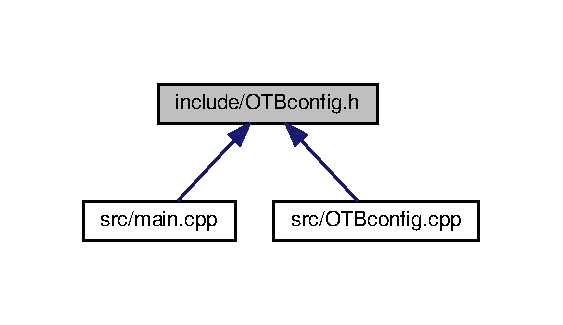
\includegraphics[width=270pt]{d4/d52/_o_t_bconfig_8h__dep__incl}
\end{center}
\end{figure}
\subsection*{Macros}
\begin{DoxyCompactItemize}
\item 
\#define \hyperlink{_o_t_bconfig_8h_aa40c2609604c572c89d9bf1063a0a08b}{C\+O\+N\+F\+I\+G\+\_\+\+S\+I\+ZE}~40
\item 
\#define \hyperlink{_o_t_bconfig_8h_abf8ef69c456ee2c69e0b31bcbbfecf46}{A\+C\+Q\+\_\+\+S\+E\+TT}~0b10000000
\item 
\#define \hyperlink{_o_t_bconfig_8h_a76df0c2a7422b57efb6bdafad46eccad}{D\+E\+C\+IM}~0b01000000
\item 
\#define \hyperlink{_o_t_bconfig_8h_a0cd1a30341827a0978898092ae67f953}{R\+E\+C\+\_\+\+ON}~0b00100000
\item 
\#define \hyperlink{_o_t_bconfig_8h_a9ace2a55b194d5503d72baedea802f68}{F\+S\+A\+M\+P1}~0b00010000
\item 
\#define \hyperlink{_o_t_bconfig_8h_afcfb59a63d197f89778038092e9e027d}{F\+S\+A\+M\+P0}~0b00001000
\item 
\#define \hyperlink{_o_t_bconfig_8h_ab2c2f4f35a5c9b00875c2ccd35c27918}{N\+C\+H1}~0b00000100
\item 
\#define \hyperlink{_o_t_bconfig_8h_ac47c5adaa9e763f6e025ee375c27737e}{N\+C\+H0}~0b00000010
\item 
\#define \hyperlink{_o_t_bconfig_8h_a2e5c538236163bd300d8105edc39d080}{A\+C\+Q\+\_\+\+ON}~0b00000001
\item 
\#define \hyperlink{_o_t_bconfig_8h_a561caad5df6dc6538cc8937b92ac1cec}{A\+C\+Q\+\_\+\+O\+FF}~0b00000000
\item 
\#define \hyperlink{_o_t_bconfig_8h_a28992f9e7ccfaebfe6190e9c1c0cef85}{F\+S\+A\+M\+P\+\_\+10240}~\hyperlink{_o_t_bconfig_8h_afcfb59a63d197f89778038092e9e027d}{F\+S\+A\+M\+P0} $\vert$ \hyperlink{_o_t_bconfig_8h_a9ace2a55b194d5503d72baedea802f68}{F\+S\+A\+M\+P1}
\item 
\#define \hyperlink{_o_t_bconfig_8h_a050cfc14b50552b50225f7e7c82966cf}{F\+S\+A\+M\+P\+\_\+5120}~\hyperlink{_o_t_bconfig_8h_a9ace2a55b194d5503d72baedea802f68}{F\+S\+A\+M\+P1}
\item 
\#define \hyperlink{_o_t_bconfig_8h_a419194a068e01fda52ab03ffa723a0a3}{F\+S\+A\+M\+P\+\_\+2048}~\hyperlink{_o_t_bconfig_8h_afcfb59a63d197f89778038092e9e027d}{F\+S\+A\+M\+P0}
\item 
\#define \hyperlink{_o_t_bconfig_8h_afed8450d6b848a2ed7c4b0df235ab416}{F\+S\+A\+M\+P\+\_\+512}~0b00000000
\item 
\#define \hyperlink{_o_t_bconfig_8h_ab3cd5ec44bca04c93dc200dd1df7a89a}{N\+C\+H\+\_\+\+I\+N1to8\+\_\+\+M\+I\+N1to4}~\hyperlink{_o_t_bconfig_8h_ab2c2f4f35a5c9b00875c2ccd35c27918}{N\+C\+H1} $\vert$ \hyperlink{_o_t_bconfig_8h_ac47c5adaa9e763f6e025ee375c27737e}{N\+C\+H0}
\item 
\#define \hyperlink{_o_t_bconfig_8h_afeb4d1e8b89c7a0de548a10967d7f0e4}{N\+C\+H\+\_\+\+I\+N1to6\+\_\+\+M\+I\+N1to3}~\hyperlink{_o_t_bconfig_8h_ab2c2f4f35a5c9b00875c2ccd35c27918}{N\+C\+H1}
\item 
\#define \hyperlink{_o_t_bconfig_8h_ab0cb172a5eebed7d9417ed2674476e7d}{N\+C\+H\+\_\+\+I\+N1to4\+\_\+\+M\+I\+N1to2}~\hyperlink{_o_t_bconfig_8h_ac47c5adaa9e763f6e025ee375c27737e}{N\+C\+H0}
\item 
\#define \hyperlink{_o_t_bconfig_8h_abf72305de541c9f7fd1b38cecc5c8d99}{N\+C\+H\+\_\+\+I\+N1to2\+\_\+\+M\+I\+N1}~0b00000000
\item 
\#define \hyperlink{_o_t_bconfig_8h_a99a2f2fcc24298540da1427d14a2c35e}{A\+N\+\_\+\+O\+U\+T\+\_\+\+I\+N\+\_\+\+S\+ET}~0b00000000
\item 
\#define \hyperlink{_o_t_bconfig_8h_a00ccf91899327b410a46ba0018d5ff1c}{A\+N\+O\+U\+T\+\_\+\+G\+A\+I\+N1}~0b00100000
\item 
\#define \hyperlink{_o_t_bconfig_8h_a5c2342a40c7c85a0308ba6c16eeab971}{A\+N\+O\+U\+T\+\_\+\+G\+A\+I\+N0}~0b00010000
\item 
\#define \hyperlink{_o_t_bconfig_8h_a586c8c1d8a9d01364f16de88a17ed683}{I\+N\+S\+E\+L3}~0b00001000
\item 
\#define \hyperlink{_o_t_bconfig_8h_aac7ffc3bc1c927ae05e72b952ffb8a62}{I\+N\+S\+E\+L2}~0b00000100
\item 
\#define \hyperlink{_o_t_bconfig_8h_a2159440217b674da25593c32eefad21f}{I\+N\+S\+E\+L1}~0b00000010
\item 
\#define \hyperlink{_o_t_bconfig_8h_adb6add05986b661f9d72d64ff4645bf8}{I\+N\+S\+E\+L0}~0b00000001
\item 
\#define \hyperlink{_o_t_bconfig_8h_afd49dca725c7a41b594f8953ceda214f}{A\+N\+O\+U\+T\+\_\+\+G\+A\+I\+N\+\_\+16}~\hyperlink{_o_t_bconfig_8h_a00ccf91899327b410a46ba0018d5ff1c}{A\+N\+O\+U\+T\+\_\+\+G\+A\+I\+N1} $\vert$ \hyperlink{_o_t_bconfig_8h_a5c2342a40c7c85a0308ba6c16eeab971}{A\+N\+O\+U\+T\+\_\+\+G\+A\+I\+N0}
\item 
\#define \hyperlink{_o_t_bconfig_8h_a56a3f8e498dc25347ba41b120e97a4e0}{A\+N\+O\+U\+T\+\_\+\+G\+A\+I\+N\+\_\+4}~\hyperlink{_o_t_bconfig_8h_a00ccf91899327b410a46ba0018d5ff1c}{A\+N\+O\+U\+T\+\_\+\+G\+A\+I\+N1}
\item 
\#define \hyperlink{_o_t_bconfig_8h_a561142f4371cfc2114f3700e4a62f78e}{A\+N\+O\+U\+T\+\_\+\+G\+A\+I\+N\+\_\+2}~\hyperlink{_o_t_bconfig_8h_a5c2342a40c7c85a0308ba6c16eeab971}{A\+N\+O\+U\+T\+\_\+\+G\+A\+I\+N0}
\item 
\#define \hyperlink{_o_t_bconfig_8h_abb34da2b242e3684e450629498468e03}{A\+N\+O\+U\+T\+\_\+\+G\+A\+I\+N\+\_\+1}~0b00000000
\item 
\#define \hyperlink{_o_t_bconfig_8h_a6ac899dddc0fac1601ce43122d3aaf64}{A\+N\+\_\+\+O\+U\+T\+\_\+\+C\+H\+\_\+\+S\+ET}~0b00000000
\item 
\#define \hyperlink{_o_t_bconfig_8h_a2d661c26ebf28219aa67677024bf504c}{C\+H\+S\+E\+L5}~0b00100000
\item 
\#define \hyperlink{_o_t_bconfig_8h_a9eed8014a0dedc64aa9e5ac9d8a21930}{C\+H\+S\+E\+L4}~0b00010000
\item 
\#define \hyperlink{_o_t_bconfig_8h_a69f28c702a9ff310dd3139133392c609}{C\+H\+S\+E\+L3}~0b00001000
\item 
\#define \hyperlink{_o_t_bconfig_8h_aa87c4771a31ea6921a42655aa0e216d1}{C\+H\+S\+E\+L2}~0b00000100
\item 
\#define \hyperlink{_o_t_bconfig_8h_a09375831fede640dc293167c04360942}{C\+H\+S\+E\+L1}~0b00000010
\item 
\#define \hyperlink{_o_t_bconfig_8h_a64a5b0b7c30345469a4e0662e422d410}{C\+H\+S\+E\+L0}~0b00000001
\item 
\#define \hyperlink{_o_t_bconfig_8h_a7fce63fe2d83e7a7f35d7b1e4d8a0c72}{I\+N\+X\+\_\+\+C\+O\+N\+F0}~0b00000000
\item 
\#define \hyperlink{_o_t_bconfig_8h_a80a895eb06cc7a6e1cf8ea039f40138d}{M\+U\+S6}~0b01000000
\item 
\#define \hyperlink{_o_t_bconfig_8h_a4ccd2ab1c48463ea0c5573325232644e}{M\+U\+S5}~0b00100000
\item 
\#define \hyperlink{_o_t_bconfig_8h_aa8c205b2dbecac6d2415412739f3b071}{M\+U\+S4}~0b00010000
\item 
\#define \hyperlink{_o_t_bconfig_8h_a5c43e6cae39ef09539eadba82fa807de}{M\+U\+S3}~0b00001000
\item 
\#define \hyperlink{_o_t_bconfig_8h_a3647e49039c6f21b88aca5173ddb1c60}{M\+U\+S2}~0b00000100
\item 
\#define \hyperlink{_o_t_bconfig_8h_af01babf4b74137c9e104f6aeee7423b4}{M\+U\+S1}~0b00000010
\item 
\#define \hyperlink{_o_t_bconfig_8h_afa01f4e2b7e4dab070cf3789a382c91e}{M\+U\+S0}~0b00000001
\item 
\#define \hyperlink{_o_t_bconfig_8h_a69507eab9cc470f7f8c4fa21a51b12ab}{Not\+\_\+defined}~0
\item 
\#define \hyperlink{_o_t_bconfig_8h_a9c70aeab0ae6b2923f339b5cb11129c6}{Temporalis\+\_\+\+Anterior}~1
\item 
\#define \hyperlink{_o_t_bconfig_8h_a72d844a6a7b478ce138b1549583abe45}{Superfic\+\_\+\+Masseter}~2
\item 
\#define \hyperlink{_o_t_bconfig_8h_a2bf26e639f4360b98901bdd42341d1eb}{Splenius\+\_\+\+Capitis}~3
\item 
\#define \hyperlink{_o_t_bconfig_8h_a6220ba59203c532abad2fa15fddfb15f}{Upper\+\_\+\+Trapezius}~4
\item 
\#define \hyperlink{_o_t_bconfig_8h_a382ccfd2716e9398589a17e3475ed36a}{Middle\+\_\+\+Trapezius}~5
\item 
\#define \hyperlink{_o_t_bconfig_8h_afc5ec77e647e113bc6dfe059f193f112}{Lower\+\_\+\+Trapezius}~6
\item 
\#define \hyperlink{_o_t_bconfig_8h_a7124ae659895bb4f04b3e777b3998bce}{Rhomboideus\+\_\+\+Major}~7
\item 
\#define \hyperlink{_o_t_bconfig_8h_ae3f79083082cec47f0d8b8dbba1c8d93}{Rhomboideus\+\_\+\+Minor}~8
\item 
\#define \hyperlink{_o_t_bconfig_8h_a8baea028eb4050eb171d146c09c2d972}{Anterior\+\_\+\+Deltoid}~9
\item 
\#define \hyperlink{_o_t_bconfig_8h_a04aca77f049582c2368de0a2ce8c3609}{Posterior\+\_\+\+Deltoid}~10
\item 
\#define \hyperlink{_o_t_bconfig_8h_a0f72c271040631ab519b3a7689bb7ab3}{Lateral\+\_\+\+Deltoid}~11
\item 
\#define \hyperlink{_o_t_bconfig_8h_acba92fb3fb11fe182a69eea1a97ce3e9}{Infraspinatus}~12
\item 
\#define \hyperlink{_o_t_bconfig_8h_a65e2d63caf558e2cb221bb2d269efa8e}{Teres\+\_\+\+Major}~13
\item 
\#define \hyperlink{_o_t_bconfig_8h_a6548c4b0e532305624ae24a7cedf609b}{Erector\+\_\+\+Spinae}~14
\item 
\#define \hyperlink{_o_t_bconfig_8h_ad657d5520d33c7c69c7a08464df41829}{Latissimus\+\_\+\+Dorsi}~15
\item 
\#define \hyperlink{_o_t_bconfig_8h_a773f33f5a7355734f395085622772464}{Bic\+\_\+\+Br\+\_\+\+Long\+\_\+\+Head}~16
\item 
\#define \hyperlink{_o_t_bconfig_8h_a11de90a9fa7f63e15de18e5c54b9e4e6}{Bic\+\_\+\+Br\+\_\+\+Short\+\_\+\+Head}~17
\item 
\#define \hyperlink{_o_t_bconfig_8h_ad536e209428882affd5135f369205d56}{Tric\+\_\+\+Br\+\_\+\+Lat\+\_\+\+Head}~18
\item 
\#define \hyperlink{_o_t_bconfig_8h_a6f6a02622dcf0faf0be5d0e677a4110f}{Tric\+\_\+\+Br\+\_\+\+Med\+\_\+\+Head}~19
\item 
\#define \hyperlink{_o_t_bconfig_8h_af296934d03f499eae15e1ea674c5b9ab}{Pronator\+\_\+\+Teres}~20
\item 
\#define \hyperlink{_o_t_bconfig_8h_abdcad84a0c154b4456b44ad59a1d21cc}{Flex\+\_\+\+Carpi\+\_\+\+Radial}~21
\item 
\#define \hyperlink{_o_t_bconfig_8h_aaffc7a2e3ddb738aad34b08784bc2e6f}{Flex\+\_\+\+Carpi\+\_\+\+Ulnaris}~22
\item 
\#define \hyperlink{_o_t_bconfig_8h_ac53502b957fc7dcffa399f95d7b175aa}{Palmaris\+\_\+\+Longus}~23
\item 
\#define \hyperlink{_o_t_bconfig_8h_ac9c9b205e2dd7dbc2854c32575b82aa4}{Ext\+\_\+\+Carpi\+\_\+\+Radialis}~24
\item 
\#define \hyperlink{_o_t_bconfig_8h_a591ecfbfc60cca732e246de2b8e1e98b}{Ext\+\_\+\+Carpi\+\_\+\+Ulnaris}~25
\item 
\#define \hyperlink{_o_t_bconfig_8h_a8f841d809960ce14fa17258f6c035556}{Ext\+\_\+\+Dig\+\_\+\+Communis}~26
\item 
\#define \hyperlink{_o_t_bconfig_8h_a8e254acb04c64ec881c1ece08e93cf13}{Brachioradialis}~27
\item 
\#define \hyperlink{_o_t_bconfig_8h_a21c0356269a3551145b78418156777ed}{Abd\+\_\+\+Pollicis\+\_\+\+Brev}~28
\item 
\#define \hyperlink{_o_t_bconfig_8h_afa5d06eee5fb6f2e4124bc33d529e4bd}{Abd\+\_\+\+Pollicis\+\_\+\+Long}~29
\item 
\#define \hyperlink{_o_t_bconfig_8h_a793aa7809dab9ca8423dcf37280f8c81}{Opponens\+\_\+\+Pollicis}~30
\item 
\#define \hyperlink{_o_t_bconfig_8h_a261aa7233de714d8a93e75f742b6f0e2}{Adductor\+\_\+\+Pollicis}~31
\item 
\#define \hyperlink{_o_t_bconfig_8h_a7f55de6a4cad1623b59f67451df95b46}{Flex\+\_\+\+Poll\+\_\+\+Brevis}~32
\item 
\#define \hyperlink{_o_t_bconfig_8h_aeeccad76a79d25577d45e2b784bfa6a9}{Abd\+\_\+\+Digiti\+\_\+\+Minimi}~33
\item 
\#define \hyperlink{_o_t_bconfig_8h_a323b29eb37153a77131f501b861ca9a0}{Flex\+\_\+\+Digiti\+\_\+\+Minimi}~34
\item 
\#define \hyperlink{_o_t_bconfig_8h_a9d511666c0cdaaa0bce6c85430edb79f}{Opp\+\_\+\+Digiti\+\_\+\+Minimi}~35
\item 
\#define \hyperlink{_o_t_bconfig_8h_aa1acc05a927e6c8e90cb1089333cfe4e}{Dorsal\+\_\+\+Interossei}~36
\item 
\#define \hyperlink{_o_t_bconfig_8h_a1b501a1f06720196d785baa0af4b3f70}{Palmar\+\_\+\+Interossei}~37
\item 
\#define \hyperlink{_o_t_bconfig_8h_a4e5549434ff726a2c7de1363d17d442a}{Lumbrical}~38
\item 
\#define \hyperlink{_o_t_bconfig_8h_a785b3d9c8b1e8932316c77ca2cb5bc94}{Rectus\+\_\+\+Abdominis}~39
\item 
\#define \hyperlink{_o_t_bconfig_8h_ac1106350376d682866bc1c99a0850ca5}{Ext\+\_\+\+Abdom\+\_\+\+Obliq}~40
\item 
\#define \hyperlink{_o_t_bconfig_8h_a4f7712ddbff9bfc0e27ef8d66010a173}{Serratus\+\_\+\+Anterior}~41
\item 
\#define \hyperlink{_o_t_bconfig_8h_a340d70c2d4d3136d42c685e6635d31bb}{Pectoralis\+\_\+\+Major}~42
\item 
\#define \hyperlink{_o_t_bconfig_8h_ab32574d9f39414d0eaa34462e570e3c1}{Sternoc\+\_\+\+Ster\+\_\+\+Head}~43
\item 
\#define \hyperlink{_o_t_bconfig_8h_a5a36506a06240d5fcdd36a2775fc35ef}{Sternoc\+\_\+\+Clav\+\_\+\+Head}~44
\item 
\#define \hyperlink{_o_t_bconfig_8h_a8acd1d668b1c0bc08a02d6d1cb72f5fe}{Anterior\+\_\+\+Scalenus}~45
\item 
\#define \hyperlink{_o_t_bconfig_8h_a9a95fa2d047fe008d6ef8918942f639e}{Tensor\+\_\+\+Fascia}~Latae 46
\item 
\#define \hyperlink{_o_t_bconfig_8h_a324cccca570774e6b7047016839d31c9}{Gastrocn\+\_\+\+Lateralis}~47
\item 
\#define \hyperlink{_o_t_bconfig_8h_ac6d81dad09094950389e7556c3a55f2b}{Gastrocn\+\_\+\+Medialis}~48
\item 
\#define \hyperlink{_o_t_bconfig_8h_a4e97531d58428adc6d1fc1850e00494c}{Biceps\+\_\+\+Femoris}~49
\item 
\#define \hyperlink{_o_t_bconfig_8h_ab502c29cb84912120fa1e52cf94e97a1}{Soleus}~50
\item 
\#define \hyperlink{_o_t_bconfig_8h_a27482a1df1085e282d55193ba24c800c}{Semitendinosus}~51
\item 
\#define \hyperlink{_o_t_bconfig_8h_ae1f8b9637b0ed0aefadc678f18cf2849}{Gluteus\+\_\+maximus}~52
\item 
\#define \hyperlink{_o_t_bconfig_8h_a8707a04c614accdb94daa77f7ed6bdf3}{Gluteus\+\_\+medius}~53
\item 
\#define \hyperlink{_o_t_bconfig_8h_af7a7b58ffa7bbcfe9bf8cc09fa064d43}{Vastus\+\_\+lateralis}~54
\item 
\#define \hyperlink{_o_t_bconfig_8h_aa1df5a0180b289f709862ad0a88c59e6}{Vastus\+\_\+medialis}~55
\item 
\#define \hyperlink{_o_t_bconfig_8h_aabc4cfc2f8a50892747ee1ee6769ac39}{Rectus\+\_\+femoris}~56
\item 
\#define \hyperlink{_o_t_bconfig_8h_ab8a20a2a44351a1bb78d2e11ef84615f}{Tibialis\+\_\+anterior}~57
\item 
\#define \hyperlink{_o_t_bconfig_8h_a6a0f0813231b945e21de26ef89ca7620}{Peroneus\+\_\+longus}~58
\item 
\#define \hyperlink{_o_t_bconfig_8h_ac1a37a49bdc903231df459c7271464fa}{Semimembranosus}~59
\item 
\#define \hyperlink{_o_t_bconfig_8h_a99df1390a9ab0ad62813d0001ff85321}{Gracilis}~60
\item 
\#define \hyperlink{_o_t_bconfig_8h_aab47559416794b1c738644d08c986fb2}{Ext\+\_\+\+Anal\+\_\+\+Sphincter}~61
\item 
\#define \hyperlink{_o_t_bconfig_8h_a2bf28130a4a5aa40cd190a19c38d9ea5}{Puborectalis}~62
\item 
\#define \hyperlink{_o_t_bconfig_8h_a46228c82f7c3c366ea966095d611fcbc}{Urethral\+\_\+\+Sphincter}~63
\item 
\#define \hyperlink{_o_t_bconfig_8h_a29a2e3c7cd0c71371c3e8863c38b975f}{Not\+\_\+a\+\_\+\+Muscle}~64
\item 
\#define \hyperlink{_o_t_bconfig_8h_ae8c793b60114ff8f8503a361ad944a81}{I\+N\+X\+\_\+\+C\+O\+N\+F1}~0b00000000
\item 
\#define \hyperlink{_o_t_bconfig_8h_aa06fd75ae78b1cfe692f0efd04938e22}{S\+E\+N\+S4}~0b10000000
\item 
\#define \hyperlink{_o_t_bconfig_8h_a909092b46eeb8a2d28993b2c0fb7bcf6}{S\+E\+N\+S3}~0b01000000
\item 
\#define \hyperlink{_o_t_bconfig_8h_a932d970452afecc0c90916f980a96cfb}{S\+E\+N\+S2}~0b00100000
\item 
\#define \hyperlink{_o_t_bconfig_8h_afe0b2f8972c40b3d096bf54fec099f2e}{S\+E\+N\+S1}~0b00010000
\item 
\#define \hyperlink{_o_t_bconfig_8h_ade2d3a8ae687e4799c3fa52357326c1c}{S\+E\+N\+S0}~0b00001000
\item 
\#define \hyperlink{_o_t_bconfig_8h_a939aaca0a1f43d13a3bee755a851a890}{A\+D\+A\+P\+T2}~0b00000100
\item 
\#define \hyperlink{_o_t_bconfig_8h_a5bf99618dce3ac6fc139865071d2c4cb}{A\+D\+A\+P\+T1}~0b00000010
\item 
\#define \hyperlink{_o_t_bconfig_8h_a3452d6b88ac3ecf70210618be16b8306}{A\+D\+A\+P\+T0}~0b00000001
\item 
\#define \hyperlink{_o_t_bconfig_8h_adc04ae0b4f80a7a9a6bebf41532eb614}{I\+N\+X\+\_\+\+C\+O\+N\+F2}~0b00000000
\item 
\#define \hyperlink{_o_t_bconfig_8h_aa5a6a673d58b0c032c7dbf2696d975b1}{S\+I\+D\+E1}~0b10000000
\item 
\#define \hyperlink{_o_t_bconfig_8h_a2f51f70b5d6a67578e1e392fa4461a1f}{S\+I\+D\+E0}~0b01000000
\item 
\#define \hyperlink{_o_t_bconfig_8h_abcf2c6045fc14b680e6f411914cd2470}{H\+P\+F1}~0b00100000
\item 
\#define \hyperlink{_o_t_bconfig_8h_aa1461bcb6b3208e7875a22bd347ce161}{H\+P\+F0}~0b00010000
\item 
\#define \hyperlink{_o_t_bconfig_8h_adb29db41670cb8956f6da3be096de461}{L\+P\+F1}~0b00001000
\item 
\#define \hyperlink{_o_t_bconfig_8h_aaee7db8d0ff40eb7f497aa25998c13cc}{L\+P\+F0}~0b00000100
\item 
\#define \hyperlink{_o_t_bconfig_8h_a443b1268c43b309560d57e34d50b5b3b}{M\+O\+D\+E1}~0b00000010
\item 
\#define \hyperlink{_o_t_bconfig_8h_a5daa4b780b82b5e8678d8c7095336b62}{M\+O\+D\+E0}~0b00000001
\item 
\#define \hyperlink{_o_t_bconfig_8h_a069795b8ae2c0050c6f8b4902c33cfd4}{S\+I\+D\+E\+\_\+\+N\+O\+NE}~\hyperlink{_o_t_bconfig_8h_aa5a6a673d58b0c032c7dbf2696d975b1}{S\+I\+D\+E1} $\vert$ \hyperlink{_o_t_bconfig_8h_a2f51f70b5d6a67578e1e392fa4461a1f}{S\+I\+D\+E0}
\item 
\#define \hyperlink{_o_t_bconfig_8h_a7063d24f8cfdeea4d2d5d9d447b8a11f}{S\+I\+D\+E\+\_\+\+R\+I\+G\+HT}~\hyperlink{_o_t_bconfig_8h_aa5a6a673d58b0c032c7dbf2696d975b1}{S\+I\+D\+E1}
\item 
\#define \hyperlink{_o_t_bconfig_8h_af0bc89249d9fa3c091578c4ff995c61c}{S\+I\+D\+E\+\_\+\+L\+E\+FT}~\hyperlink{_o_t_bconfig_8h_a2f51f70b5d6a67578e1e392fa4461a1f}{S\+I\+D\+E0}
\item 
\#define \hyperlink{_o_t_bconfig_8h_a7125abaef3a79df497a118bd55657c28}{S\+I\+D\+E\+\_\+\+U\+N\+D\+E\+F\+I\+N\+ED}~0b00000000
\item 
\#define \hyperlink{_o_t_bconfig_8h_a4e6888ed350a8125d2adf7de20298256}{H\+I\+G\+H\+\_\+\+P\+A\+S\+S\+\_\+\+F\+I\+L\+T\+E\+R\+\_\+200}~\hyperlink{_o_t_bconfig_8h_abcf2c6045fc14b680e6f411914cd2470}{H\+P\+F1} $\vert$ \hyperlink{_o_t_bconfig_8h_aa1461bcb6b3208e7875a22bd347ce161}{H\+P\+F0}
\item 
\#define \hyperlink{_o_t_bconfig_8h_ad058d5e8813dd2d486d4abab03096508}{H\+I\+G\+H\+\_\+\+P\+A\+S\+S\+\_\+\+F\+I\+L\+T\+E\+R\+\_\+100}~\hyperlink{_o_t_bconfig_8h_abcf2c6045fc14b680e6f411914cd2470}{H\+P\+F1}
\item 
\#define \hyperlink{_o_t_bconfig_8h_ab456194a2b584c2ebed1134d0c9523f2}{H\+I\+G\+H\+\_\+\+P\+A\+S\+S\+\_\+\+F\+I\+L\+T\+E\+R\+\_\+10}~\hyperlink{_o_t_bconfig_8h_aa1461bcb6b3208e7875a22bd347ce161}{H\+P\+F0}
\item 
\#define \hyperlink{_o_t_bconfig_8h_aca80274b2ccc1075a747c08c2e80da35}{H\+I\+G\+H\+\_\+\+P\+A\+S\+S\+\_\+\+F\+I\+L\+T\+E\+R\+\_\+03}~0b00000000
\item 
\#define \hyperlink{_o_t_bconfig_8h_a6108fa402e1e0e0fec9418495d4ee208}{L\+O\+W\+\_\+\+P\+A\+S\+S\+\_\+\+F\+I\+L\+T\+E\+R\+\_\+4400}~\hyperlink{_o_t_bconfig_8h_adb29db41670cb8956f6da3be096de461}{L\+P\+F1} $\vert$ \hyperlink{_o_t_bconfig_8h_aaee7db8d0ff40eb7f497aa25998c13cc}{L\+P\+F0}
\item 
\#define \hyperlink{_o_t_bconfig_8h_abc6fa382ab3a2ab594038e0d35bdc874}{L\+O\+W\+\_\+\+P\+A\+S\+S\+\_\+\+F\+I\+L\+T\+E\+R\+\_\+900}~\hyperlink{_o_t_bconfig_8h_adb29db41670cb8956f6da3be096de461}{L\+P\+F1}
\item 
\#define \hyperlink{_o_t_bconfig_8h_ad8c3a1441a96b6af1b4338b306e497e7}{L\+O\+W\+\_\+\+P\+A\+S\+S\+\_\+\+F\+I\+L\+T\+E\+R\+\_\+500}~\hyperlink{_o_t_bconfig_8h_aaee7db8d0ff40eb7f497aa25998c13cc}{L\+P\+F0}
\item 
\#define \hyperlink{_o_t_bconfig_8h_aaf2d77d3b45c499db00e9a1f1eafeae6}{L\+O\+W\+\_\+\+P\+A\+S\+S\+\_\+\+F\+I\+L\+T\+E\+R\+\_\+130}~0b00000000
\item 
\#define \hyperlink{_o_t_bconfig_8h_a4c9dee6a6de692f2896c5fc0d4e247a4}{D\+E\+T\+E\+C\+T\+I\+O\+N\+\_\+\+M\+O\+D\+E\+\_\+\+B\+I\+P\+O\+L\+AR}~\hyperlink{_o_t_bconfig_8h_a443b1268c43b309560d57e34d50b5b3b}{M\+O\+D\+E1}
\item 
\#define \hyperlink{_o_t_bconfig_8h_a13d0cb34c330e7b5810e9076f3ee1b72}{D\+E\+T\+E\+C\+T\+I\+O\+N\+\_\+\+M\+O\+D\+E\+\_\+\+D\+I\+F\+F\+E\+R\+E\+N\+C\+I\+AL}~\hyperlink{_o_t_bconfig_8h_a5daa4b780b82b5e8678d8c7095336b62}{M\+O\+D\+E0}
\item 
\#define \hyperlink{_o_t_bconfig_8h_a131e3f6a86f4c81571ec3ecefe27d877}{D\+E\+T\+E\+C\+T\+I\+O\+N\+\_\+\+M\+O\+D\+E\+\_\+\+M\+O\+N\+O\+P\+O\+L\+AR}~0b00000000
\item 
\#define \hyperlink{_o_t_bconfig_8h_a690a7565f5c52ec1176048e29c22baae}{C\+R\+C\+\_\+\+C\+O\+DE}~0b10001100
\end{DoxyCompactItemize}
\subsection*{Functions}
\begin{DoxyCompactItemize}
\item 
unsigned char \hyperlink{_o_t_bconfig_8h_a0596e4e702611a9eb9b7944b5e8d2052}{crc} (unsigned char config\mbox{[}$\,$\mbox{]})
\item 
void \hyperlink{_o_t_bconfig_8h_a559d96e1efb00e2d877fe600280e75f7}{print\+B\+IN} (char)
\end{DoxyCompactItemize}


\subsection{Macro Definition Documentation}
\mbox{\Hypertarget{_o_t_bconfig_8h_aeeccad76a79d25577d45e2b784bfa6a9}\label{_o_t_bconfig_8h_aeeccad76a79d25577d45e2b784bfa6a9}} 
\index{O\+T\+Bconfig.\+h@{O\+T\+Bconfig.\+h}!Abd\+\_\+\+Digiti\+\_\+\+Minimi@{Abd\+\_\+\+Digiti\+\_\+\+Minimi}}
\index{Abd\+\_\+\+Digiti\+\_\+\+Minimi@{Abd\+\_\+\+Digiti\+\_\+\+Minimi}!O\+T\+Bconfig.\+h@{O\+T\+Bconfig.\+h}}
\subsubsection{\texorpdfstring{Abd\+\_\+\+Digiti\+\_\+\+Minimi}{Abd\_Digiti\_Minimi}}
{\footnotesize\ttfamily \#define Abd\+\_\+\+Digiti\+\_\+\+Minimi~33}

\mbox{\Hypertarget{_o_t_bconfig_8h_a21c0356269a3551145b78418156777ed}\label{_o_t_bconfig_8h_a21c0356269a3551145b78418156777ed}} 
\index{O\+T\+Bconfig.\+h@{O\+T\+Bconfig.\+h}!Abd\+\_\+\+Pollicis\+\_\+\+Brev@{Abd\+\_\+\+Pollicis\+\_\+\+Brev}}
\index{Abd\+\_\+\+Pollicis\+\_\+\+Brev@{Abd\+\_\+\+Pollicis\+\_\+\+Brev}!O\+T\+Bconfig.\+h@{O\+T\+Bconfig.\+h}}
\subsubsection{\texorpdfstring{Abd\+\_\+\+Pollicis\+\_\+\+Brev}{Abd\_Pollicis\_Brev}}
{\footnotesize\ttfamily \#define Abd\+\_\+\+Pollicis\+\_\+\+Brev~28}

\mbox{\Hypertarget{_o_t_bconfig_8h_afa5d06eee5fb6f2e4124bc33d529e4bd}\label{_o_t_bconfig_8h_afa5d06eee5fb6f2e4124bc33d529e4bd}} 
\index{O\+T\+Bconfig.\+h@{O\+T\+Bconfig.\+h}!Abd\+\_\+\+Pollicis\+\_\+\+Long@{Abd\+\_\+\+Pollicis\+\_\+\+Long}}
\index{Abd\+\_\+\+Pollicis\+\_\+\+Long@{Abd\+\_\+\+Pollicis\+\_\+\+Long}!O\+T\+Bconfig.\+h@{O\+T\+Bconfig.\+h}}
\subsubsection{\texorpdfstring{Abd\+\_\+\+Pollicis\+\_\+\+Long}{Abd\_Pollicis\_Long}}
{\footnotesize\ttfamily \#define Abd\+\_\+\+Pollicis\+\_\+\+Long~29}

\mbox{\Hypertarget{_o_t_bconfig_8h_a561caad5df6dc6538cc8937b92ac1cec}\label{_o_t_bconfig_8h_a561caad5df6dc6538cc8937b92ac1cec}} 
\index{O\+T\+Bconfig.\+h@{O\+T\+Bconfig.\+h}!A\+C\+Q\+\_\+\+O\+FF@{A\+C\+Q\+\_\+\+O\+FF}}
\index{A\+C\+Q\+\_\+\+O\+FF@{A\+C\+Q\+\_\+\+O\+FF}!O\+T\+Bconfig.\+h@{O\+T\+Bconfig.\+h}}
\subsubsection{\texorpdfstring{A\+C\+Q\+\_\+\+O\+FF}{ACQ\_OFF}}
{\footnotesize\ttfamily \#define A\+C\+Q\+\_\+\+O\+FF~0b00000000}

\mbox{\Hypertarget{_o_t_bconfig_8h_a2e5c538236163bd300d8105edc39d080}\label{_o_t_bconfig_8h_a2e5c538236163bd300d8105edc39d080}} 
\index{O\+T\+Bconfig.\+h@{O\+T\+Bconfig.\+h}!A\+C\+Q\+\_\+\+ON@{A\+C\+Q\+\_\+\+ON}}
\index{A\+C\+Q\+\_\+\+ON@{A\+C\+Q\+\_\+\+ON}!O\+T\+Bconfig.\+h@{O\+T\+Bconfig.\+h}}
\subsubsection{\texorpdfstring{A\+C\+Q\+\_\+\+ON}{ACQ\_ON}}
{\footnotesize\ttfamily \#define A\+C\+Q\+\_\+\+ON~0b00000001}

\mbox{\Hypertarget{_o_t_bconfig_8h_abf8ef69c456ee2c69e0b31bcbbfecf46}\label{_o_t_bconfig_8h_abf8ef69c456ee2c69e0b31bcbbfecf46}} 
\index{O\+T\+Bconfig.\+h@{O\+T\+Bconfig.\+h}!A\+C\+Q\+\_\+\+S\+E\+TT@{A\+C\+Q\+\_\+\+S\+E\+TT}}
\index{A\+C\+Q\+\_\+\+S\+E\+TT@{A\+C\+Q\+\_\+\+S\+E\+TT}!O\+T\+Bconfig.\+h@{O\+T\+Bconfig.\+h}}
\subsubsection{\texorpdfstring{A\+C\+Q\+\_\+\+S\+E\+TT}{ACQ\_SETT}}
{\footnotesize\ttfamily \#define A\+C\+Q\+\_\+\+S\+E\+TT~0b10000000}

\mbox{\Hypertarget{_o_t_bconfig_8h_a3452d6b88ac3ecf70210618be16b8306}\label{_o_t_bconfig_8h_a3452d6b88ac3ecf70210618be16b8306}} 
\index{O\+T\+Bconfig.\+h@{O\+T\+Bconfig.\+h}!A\+D\+A\+P\+T0@{A\+D\+A\+P\+T0}}
\index{A\+D\+A\+P\+T0@{A\+D\+A\+P\+T0}!O\+T\+Bconfig.\+h@{O\+T\+Bconfig.\+h}}
\subsubsection{\texorpdfstring{A\+D\+A\+P\+T0}{ADAPT0}}
{\footnotesize\ttfamily \#define A\+D\+A\+P\+T0~0b00000001}

\mbox{\Hypertarget{_o_t_bconfig_8h_a5bf99618dce3ac6fc139865071d2c4cb}\label{_o_t_bconfig_8h_a5bf99618dce3ac6fc139865071d2c4cb}} 
\index{O\+T\+Bconfig.\+h@{O\+T\+Bconfig.\+h}!A\+D\+A\+P\+T1@{A\+D\+A\+P\+T1}}
\index{A\+D\+A\+P\+T1@{A\+D\+A\+P\+T1}!O\+T\+Bconfig.\+h@{O\+T\+Bconfig.\+h}}
\subsubsection{\texorpdfstring{A\+D\+A\+P\+T1}{ADAPT1}}
{\footnotesize\ttfamily \#define A\+D\+A\+P\+T1~0b00000010}

\mbox{\Hypertarget{_o_t_bconfig_8h_a939aaca0a1f43d13a3bee755a851a890}\label{_o_t_bconfig_8h_a939aaca0a1f43d13a3bee755a851a890}} 
\index{O\+T\+Bconfig.\+h@{O\+T\+Bconfig.\+h}!A\+D\+A\+P\+T2@{A\+D\+A\+P\+T2}}
\index{A\+D\+A\+P\+T2@{A\+D\+A\+P\+T2}!O\+T\+Bconfig.\+h@{O\+T\+Bconfig.\+h}}
\subsubsection{\texorpdfstring{A\+D\+A\+P\+T2}{ADAPT2}}
{\footnotesize\ttfamily \#define A\+D\+A\+P\+T2~0b00000100}

\mbox{\Hypertarget{_o_t_bconfig_8h_a261aa7233de714d8a93e75f742b6f0e2}\label{_o_t_bconfig_8h_a261aa7233de714d8a93e75f742b6f0e2}} 
\index{O\+T\+Bconfig.\+h@{O\+T\+Bconfig.\+h}!Adductor\+\_\+\+Pollicis@{Adductor\+\_\+\+Pollicis}}
\index{Adductor\+\_\+\+Pollicis@{Adductor\+\_\+\+Pollicis}!O\+T\+Bconfig.\+h@{O\+T\+Bconfig.\+h}}
\subsubsection{\texorpdfstring{Adductor\+\_\+\+Pollicis}{Adductor\_Pollicis}}
{\footnotesize\ttfamily \#define Adductor\+\_\+\+Pollicis~31}

\mbox{\Hypertarget{_o_t_bconfig_8h_a6ac899dddc0fac1601ce43122d3aaf64}\label{_o_t_bconfig_8h_a6ac899dddc0fac1601ce43122d3aaf64}} 
\index{O\+T\+Bconfig.\+h@{O\+T\+Bconfig.\+h}!A\+N\+\_\+\+O\+U\+T\+\_\+\+C\+H\+\_\+\+S\+ET@{A\+N\+\_\+\+O\+U\+T\+\_\+\+C\+H\+\_\+\+S\+ET}}
\index{A\+N\+\_\+\+O\+U\+T\+\_\+\+C\+H\+\_\+\+S\+ET@{A\+N\+\_\+\+O\+U\+T\+\_\+\+C\+H\+\_\+\+S\+ET}!O\+T\+Bconfig.\+h@{O\+T\+Bconfig.\+h}}
\subsubsection{\texorpdfstring{A\+N\+\_\+\+O\+U\+T\+\_\+\+C\+H\+\_\+\+S\+ET}{AN\_OUT\_CH\_SET}}
{\footnotesize\ttfamily \#define A\+N\+\_\+\+O\+U\+T\+\_\+\+C\+H\+\_\+\+S\+ET~0b00000000}

\mbox{\Hypertarget{_o_t_bconfig_8h_a99a2f2fcc24298540da1427d14a2c35e}\label{_o_t_bconfig_8h_a99a2f2fcc24298540da1427d14a2c35e}} 
\index{O\+T\+Bconfig.\+h@{O\+T\+Bconfig.\+h}!A\+N\+\_\+\+O\+U\+T\+\_\+\+I\+N\+\_\+\+S\+ET@{A\+N\+\_\+\+O\+U\+T\+\_\+\+I\+N\+\_\+\+S\+ET}}
\index{A\+N\+\_\+\+O\+U\+T\+\_\+\+I\+N\+\_\+\+S\+ET@{A\+N\+\_\+\+O\+U\+T\+\_\+\+I\+N\+\_\+\+S\+ET}!O\+T\+Bconfig.\+h@{O\+T\+Bconfig.\+h}}
\subsubsection{\texorpdfstring{A\+N\+\_\+\+O\+U\+T\+\_\+\+I\+N\+\_\+\+S\+ET}{AN\_OUT\_IN\_SET}}
{\footnotesize\ttfamily \#define A\+N\+\_\+\+O\+U\+T\+\_\+\+I\+N\+\_\+\+S\+ET~0b00000000}

\mbox{\Hypertarget{_o_t_bconfig_8h_a5c2342a40c7c85a0308ba6c16eeab971}\label{_o_t_bconfig_8h_a5c2342a40c7c85a0308ba6c16eeab971}} 
\index{O\+T\+Bconfig.\+h@{O\+T\+Bconfig.\+h}!A\+N\+O\+U\+T\+\_\+\+G\+A\+I\+N0@{A\+N\+O\+U\+T\+\_\+\+G\+A\+I\+N0}}
\index{A\+N\+O\+U\+T\+\_\+\+G\+A\+I\+N0@{A\+N\+O\+U\+T\+\_\+\+G\+A\+I\+N0}!O\+T\+Bconfig.\+h@{O\+T\+Bconfig.\+h}}
\subsubsection{\texorpdfstring{A\+N\+O\+U\+T\+\_\+\+G\+A\+I\+N0}{ANOUT\_GAIN0}}
{\footnotesize\ttfamily \#define A\+N\+O\+U\+T\+\_\+\+G\+A\+I\+N0~0b00010000}

\mbox{\Hypertarget{_o_t_bconfig_8h_a00ccf91899327b410a46ba0018d5ff1c}\label{_o_t_bconfig_8h_a00ccf91899327b410a46ba0018d5ff1c}} 
\index{O\+T\+Bconfig.\+h@{O\+T\+Bconfig.\+h}!A\+N\+O\+U\+T\+\_\+\+G\+A\+I\+N1@{A\+N\+O\+U\+T\+\_\+\+G\+A\+I\+N1}}
\index{A\+N\+O\+U\+T\+\_\+\+G\+A\+I\+N1@{A\+N\+O\+U\+T\+\_\+\+G\+A\+I\+N1}!O\+T\+Bconfig.\+h@{O\+T\+Bconfig.\+h}}
\subsubsection{\texorpdfstring{A\+N\+O\+U\+T\+\_\+\+G\+A\+I\+N1}{ANOUT\_GAIN1}}
{\footnotesize\ttfamily \#define A\+N\+O\+U\+T\+\_\+\+G\+A\+I\+N1~0b00100000}

\mbox{\Hypertarget{_o_t_bconfig_8h_abb34da2b242e3684e450629498468e03}\label{_o_t_bconfig_8h_abb34da2b242e3684e450629498468e03}} 
\index{O\+T\+Bconfig.\+h@{O\+T\+Bconfig.\+h}!A\+N\+O\+U\+T\+\_\+\+G\+A\+I\+N\+\_\+1@{A\+N\+O\+U\+T\+\_\+\+G\+A\+I\+N\+\_\+1}}
\index{A\+N\+O\+U\+T\+\_\+\+G\+A\+I\+N\+\_\+1@{A\+N\+O\+U\+T\+\_\+\+G\+A\+I\+N\+\_\+1}!O\+T\+Bconfig.\+h@{O\+T\+Bconfig.\+h}}
\subsubsection{\texorpdfstring{A\+N\+O\+U\+T\+\_\+\+G\+A\+I\+N\+\_\+1}{ANOUT\_GAIN\_1}}
{\footnotesize\ttfamily \#define A\+N\+O\+U\+T\+\_\+\+G\+A\+I\+N\+\_\+1~0b00000000}

\mbox{\Hypertarget{_o_t_bconfig_8h_afd49dca725c7a41b594f8953ceda214f}\label{_o_t_bconfig_8h_afd49dca725c7a41b594f8953ceda214f}} 
\index{O\+T\+Bconfig.\+h@{O\+T\+Bconfig.\+h}!A\+N\+O\+U\+T\+\_\+\+G\+A\+I\+N\+\_\+16@{A\+N\+O\+U\+T\+\_\+\+G\+A\+I\+N\+\_\+16}}
\index{A\+N\+O\+U\+T\+\_\+\+G\+A\+I\+N\+\_\+16@{A\+N\+O\+U\+T\+\_\+\+G\+A\+I\+N\+\_\+16}!O\+T\+Bconfig.\+h@{O\+T\+Bconfig.\+h}}
\subsubsection{\texorpdfstring{A\+N\+O\+U\+T\+\_\+\+G\+A\+I\+N\+\_\+16}{ANOUT\_GAIN\_16}}
{\footnotesize\ttfamily \#define A\+N\+O\+U\+T\+\_\+\+G\+A\+I\+N\+\_\+16~\hyperlink{_o_t_bconfig_8h_a00ccf91899327b410a46ba0018d5ff1c}{A\+N\+O\+U\+T\+\_\+\+G\+A\+I\+N1} $\vert$ \hyperlink{_o_t_bconfig_8h_a5c2342a40c7c85a0308ba6c16eeab971}{A\+N\+O\+U\+T\+\_\+\+G\+A\+I\+N0}}

\mbox{\Hypertarget{_o_t_bconfig_8h_a561142f4371cfc2114f3700e4a62f78e}\label{_o_t_bconfig_8h_a561142f4371cfc2114f3700e4a62f78e}} 
\index{O\+T\+Bconfig.\+h@{O\+T\+Bconfig.\+h}!A\+N\+O\+U\+T\+\_\+\+G\+A\+I\+N\+\_\+2@{A\+N\+O\+U\+T\+\_\+\+G\+A\+I\+N\+\_\+2}}
\index{A\+N\+O\+U\+T\+\_\+\+G\+A\+I\+N\+\_\+2@{A\+N\+O\+U\+T\+\_\+\+G\+A\+I\+N\+\_\+2}!O\+T\+Bconfig.\+h@{O\+T\+Bconfig.\+h}}
\subsubsection{\texorpdfstring{A\+N\+O\+U\+T\+\_\+\+G\+A\+I\+N\+\_\+2}{ANOUT\_GAIN\_2}}
{\footnotesize\ttfamily \#define A\+N\+O\+U\+T\+\_\+\+G\+A\+I\+N\+\_\+2~\hyperlink{_o_t_bconfig_8h_a5c2342a40c7c85a0308ba6c16eeab971}{A\+N\+O\+U\+T\+\_\+\+G\+A\+I\+N0}}

\mbox{\Hypertarget{_o_t_bconfig_8h_a56a3f8e498dc25347ba41b120e97a4e0}\label{_o_t_bconfig_8h_a56a3f8e498dc25347ba41b120e97a4e0}} 
\index{O\+T\+Bconfig.\+h@{O\+T\+Bconfig.\+h}!A\+N\+O\+U\+T\+\_\+\+G\+A\+I\+N\+\_\+4@{A\+N\+O\+U\+T\+\_\+\+G\+A\+I\+N\+\_\+4}}
\index{A\+N\+O\+U\+T\+\_\+\+G\+A\+I\+N\+\_\+4@{A\+N\+O\+U\+T\+\_\+\+G\+A\+I\+N\+\_\+4}!O\+T\+Bconfig.\+h@{O\+T\+Bconfig.\+h}}
\subsubsection{\texorpdfstring{A\+N\+O\+U\+T\+\_\+\+G\+A\+I\+N\+\_\+4}{ANOUT\_GAIN\_4}}
{\footnotesize\ttfamily \#define A\+N\+O\+U\+T\+\_\+\+G\+A\+I\+N\+\_\+4~\hyperlink{_o_t_bconfig_8h_a00ccf91899327b410a46ba0018d5ff1c}{A\+N\+O\+U\+T\+\_\+\+G\+A\+I\+N1}}

\mbox{\Hypertarget{_o_t_bconfig_8h_a8baea028eb4050eb171d146c09c2d972}\label{_o_t_bconfig_8h_a8baea028eb4050eb171d146c09c2d972}} 
\index{O\+T\+Bconfig.\+h@{O\+T\+Bconfig.\+h}!Anterior\+\_\+\+Deltoid@{Anterior\+\_\+\+Deltoid}}
\index{Anterior\+\_\+\+Deltoid@{Anterior\+\_\+\+Deltoid}!O\+T\+Bconfig.\+h@{O\+T\+Bconfig.\+h}}
\subsubsection{\texorpdfstring{Anterior\+\_\+\+Deltoid}{Anterior\_Deltoid}}
{\footnotesize\ttfamily \#define Anterior\+\_\+\+Deltoid~9}

\mbox{\Hypertarget{_o_t_bconfig_8h_a8acd1d668b1c0bc08a02d6d1cb72f5fe}\label{_o_t_bconfig_8h_a8acd1d668b1c0bc08a02d6d1cb72f5fe}} 
\index{O\+T\+Bconfig.\+h@{O\+T\+Bconfig.\+h}!Anterior\+\_\+\+Scalenus@{Anterior\+\_\+\+Scalenus}}
\index{Anterior\+\_\+\+Scalenus@{Anterior\+\_\+\+Scalenus}!O\+T\+Bconfig.\+h@{O\+T\+Bconfig.\+h}}
\subsubsection{\texorpdfstring{Anterior\+\_\+\+Scalenus}{Anterior\_Scalenus}}
{\footnotesize\ttfamily \#define Anterior\+\_\+\+Scalenus~45}

\mbox{\Hypertarget{_o_t_bconfig_8h_a773f33f5a7355734f395085622772464}\label{_o_t_bconfig_8h_a773f33f5a7355734f395085622772464}} 
\index{O\+T\+Bconfig.\+h@{O\+T\+Bconfig.\+h}!Bic\+\_\+\+Br\+\_\+\+Long\+\_\+\+Head@{Bic\+\_\+\+Br\+\_\+\+Long\+\_\+\+Head}}
\index{Bic\+\_\+\+Br\+\_\+\+Long\+\_\+\+Head@{Bic\+\_\+\+Br\+\_\+\+Long\+\_\+\+Head}!O\+T\+Bconfig.\+h@{O\+T\+Bconfig.\+h}}
\subsubsection{\texorpdfstring{Bic\+\_\+\+Br\+\_\+\+Long\+\_\+\+Head}{Bic\_Br\_Long\_Head}}
{\footnotesize\ttfamily \#define Bic\+\_\+\+Br\+\_\+\+Long\+\_\+\+Head~16}

\mbox{\Hypertarget{_o_t_bconfig_8h_a11de90a9fa7f63e15de18e5c54b9e4e6}\label{_o_t_bconfig_8h_a11de90a9fa7f63e15de18e5c54b9e4e6}} 
\index{O\+T\+Bconfig.\+h@{O\+T\+Bconfig.\+h}!Bic\+\_\+\+Br\+\_\+\+Short\+\_\+\+Head@{Bic\+\_\+\+Br\+\_\+\+Short\+\_\+\+Head}}
\index{Bic\+\_\+\+Br\+\_\+\+Short\+\_\+\+Head@{Bic\+\_\+\+Br\+\_\+\+Short\+\_\+\+Head}!O\+T\+Bconfig.\+h@{O\+T\+Bconfig.\+h}}
\subsubsection{\texorpdfstring{Bic\+\_\+\+Br\+\_\+\+Short\+\_\+\+Head}{Bic\_Br\_Short\_Head}}
{\footnotesize\ttfamily \#define Bic\+\_\+\+Br\+\_\+\+Short\+\_\+\+Head~17}

\mbox{\Hypertarget{_o_t_bconfig_8h_a4e97531d58428adc6d1fc1850e00494c}\label{_o_t_bconfig_8h_a4e97531d58428adc6d1fc1850e00494c}} 
\index{O\+T\+Bconfig.\+h@{O\+T\+Bconfig.\+h}!Biceps\+\_\+\+Femoris@{Biceps\+\_\+\+Femoris}}
\index{Biceps\+\_\+\+Femoris@{Biceps\+\_\+\+Femoris}!O\+T\+Bconfig.\+h@{O\+T\+Bconfig.\+h}}
\subsubsection{\texorpdfstring{Biceps\+\_\+\+Femoris}{Biceps\_Femoris}}
{\footnotesize\ttfamily \#define Biceps\+\_\+\+Femoris~49}

\mbox{\Hypertarget{_o_t_bconfig_8h_a8e254acb04c64ec881c1ece08e93cf13}\label{_o_t_bconfig_8h_a8e254acb04c64ec881c1ece08e93cf13}} 
\index{O\+T\+Bconfig.\+h@{O\+T\+Bconfig.\+h}!Brachioradialis@{Brachioradialis}}
\index{Brachioradialis@{Brachioradialis}!O\+T\+Bconfig.\+h@{O\+T\+Bconfig.\+h}}
\subsubsection{\texorpdfstring{Brachioradialis}{Brachioradialis}}
{\footnotesize\ttfamily \#define Brachioradialis~27}

\mbox{\Hypertarget{_o_t_bconfig_8h_a64a5b0b7c30345469a4e0662e422d410}\label{_o_t_bconfig_8h_a64a5b0b7c30345469a4e0662e422d410}} 
\index{O\+T\+Bconfig.\+h@{O\+T\+Bconfig.\+h}!C\+H\+S\+E\+L0@{C\+H\+S\+E\+L0}}
\index{C\+H\+S\+E\+L0@{C\+H\+S\+E\+L0}!O\+T\+Bconfig.\+h@{O\+T\+Bconfig.\+h}}
\subsubsection{\texorpdfstring{C\+H\+S\+E\+L0}{CHSEL0}}
{\footnotesize\ttfamily \#define C\+H\+S\+E\+L0~0b00000001}

\mbox{\Hypertarget{_o_t_bconfig_8h_a09375831fede640dc293167c04360942}\label{_o_t_bconfig_8h_a09375831fede640dc293167c04360942}} 
\index{O\+T\+Bconfig.\+h@{O\+T\+Bconfig.\+h}!C\+H\+S\+E\+L1@{C\+H\+S\+E\+L1}}
\index{C\+H\+S\+E\+L1@{C\+H\+S\+E\+L1}!O\+T\+Bconfig.\+h@{O\+T\+Bconfig.\+h}}
\subsubsection{\texorpdfstring{C\+H\+S\+E\+L1}{CHSEL1}}
{\footnotesize\ttfamily \#define C\+H\+S\+E\+L1~0b00000010}

\mbox{\Hypertarget{_o_t_bconfig_8h_aa87c4771a31ea6921a42655aa0e216d1}\label{_o_t_bconfig_8h_aa87c4771a31ea6921a42655aa0e216d1}} 
\index{O\+T\+Bconfig.\+h@{O\+T\+Bconfig.\+h}!C\+H\+S\+E\+L2@{C\+H\+S\+E\+L2}}
\index{C\+H\+S\+E\+L2@{C\+H\+S\+E\+L2}!O\+T\+Bconfig.\+h@{O\+T\+Bconfig.\+h}}
\subsubsection{\texorpdfstring{C\+H\+S\+E\+L2}{CHSEL2}}
{\footnotesize\ttfamily \#define C\+H\+S\+E\+L2~0b00000100}

\mbox{\Hypertarget{_o_t_bconfig_8h_a69f28c702a9ff310dd3139133392c609}\label{_o_t_bconfig_8h_a69f28c702a9ff310dd3139133392c609}} 
\index{O\+T\+Bconfig.\+h@{O\+T\+Bconfig.\+h}!C\+H\+S\+E\+L3@{C\+H\+S\+E\+L3}}
\index{C\+H\+S\+E\+L3@{C\+H\+S\+E\+L3}!O\+T\+Bconfig.\+h@{O\+T\+Bconfig.\+h}}
\subsubsection{\texorpdfstring{C\+H\+S\+E\+L3}{CHSEL3}}
{\footnotesize\ttfamily \#define C\+H\+S\+E\+L3~0b00001000}

\mbox{\Hypertarget{_o_t_bconfig_8h_a9eed8014a0dedc64aa9e5ac9d8a21930}\label{_o_t_bconfig_8h_a9eed8014a0dedc64aa9e5ac9d8a21930}} 
\index{O\+T\+Bconfig.\+h@{O\+T\+Bconfig.\+h}!C\+H\+S\+E\+L4@{C\+H\+S\+E\+L4}}
\index{C\+H\+S\+E\+L4@{C\+H\+S\+E\+L4}!O\+T\+Bconfig.\+h@{O\+T\+Bconfig.\+h}}
\subsubsection{\texorpdfstring{C\+H\+S\+E\+L4}{CHSEL4}}
{\footnotesize\ttfamily \#define C\+H\+S\+E\+L4~0b00010000}

\mbox{\Hypertarget{_o_t_bconfig_8h_a2d661c26ebf28219aa67677024bf504c}\label{_o_t_bconfig_8h_a2d661c26ebf28219aa67677024bf504c}} 
\index{O\+T\+Bconfig.\+h@{O\+T\+Bconfig.\+h}!C\+H\+S\+E\+L5@{C\+H\+S\+E\+L5}}
\index{C\+H\+S\+E\+L5@{C\+H\+S\+E\+L5}!O\+T\+Bconfig.\+h@{O\+T\+Bconfig.\+h}}
\subsubsection{\texorpdfstring{C\+H\+S\+E\+L5}{CHSEL5}}
{\footnotesize\ttfamily \#define C\+H\+S\+E\+L5~0b00100000}

\mbox{\Hypertarget{_o_t_bconfig_8h_aa40c2609604c572c89d9bf1063a0a08b}\label{_o_t_bconfig_8h_aa40c2609604c572c89d9bf1063a0a08b}} 
\index{O\+T\+Bconfig.\+h@{O\+T\+Bconfig.\+h}!C\+O\+N\+F\+I\+G\+\_\+\+S\+I\+ZE@{C\+O\+N\+F\+I\+G\+\_\+\+S\+I\+ZE}}
\index{C\+O\+N\+F\+I\+G\+\_\+\+S\+I\+ZE@{C\+O\+N\+F\+I\+G\+\_\+\+S\+I\+ZE}!O\+T\+Bconfig.\+h@{O\+T\+Bconfig.\+h}}
\subsubsection{\texorpdfstring{C\+O\+N\+F\+I\+G\+\_\+\+S\+I\+ZE}{CONFIG\_SIZE}}
{\footnotesize\ttfamily \#define C\+O\+N\+F\+I\+G\+\_\+\+S\+I\+ZE~40}

\mbox{\Hypertarget{_o_t_bconfig_8h_a690a7565f5c52ec1176048e29c22baae}\label{_o_t_bconfig_8h_a690a7565f5c52ec1176048e29c22baae}} 
\index{O\+T\+Bconfig.\+h@{O\+T\+Bconfig.\+h}!C\+R\+C\+\_\+\+C\+O\+DE@{C\+R\+C\+\_\+\+C\+O\+DE}}
\index{C\+R\+C\+\_\+\+C\+O\+DE@{C\+R\+C\+\_\+\+C\+O\+DE}!O\+T\+Bconfig.\+h@{O\+T\+Bconfig.\+h}}
\subsubsection{\texorpdfstring{C\+R\+C\+\_\+\+C\+O\+DE}{CRC\_CODE}}
{\footnotesize\ttfamily \#define C\+R\+C\+\_\+\+C\+O\+DE~0b10001100}

\mbox{\Hypertarget{_o_t_bconfig_8h_a76df0c2a7422b57efb6bdafad46eccad}\label{_o_t_bconfig_8h_a76df0c2a7422b57efb6bdafad46eccad}} 
\index{O\+T\+Bconfig.\+h@{O\+T\+Bconfig.\+h}!D\+E\+C\+IM@{D\+E\+C\+IM}}
\index{D\+E\+C\+IM@{D\+E\+C\+IM}!O\+T\+Bconfig.\+h@{O\+T\+Bconfig.\+h}}
\subsubsection{\texorpdfstring{D\+E\+C\+IM}{DECIM}}
{\footnotesize\ttfamily \#define D\+E\+C\+IM~0b01000000}

\mbox{\Hypertarget{_o_t_bconfig_8h_a4c9dee6a6de692f2896c5fc0d4e247a4}\label{_o_t_bconfig_8h_a4c9dee6a6de692f2896c5fc0d4e247a4}} 
\index{O\+T\+Bconfig.\+h@{O\+T\+Bconfig.\+h}!D\+E\+T\+E\+C\+T\+I\+O\+N\+\_\+\+M\+O\+D\+E\+\_\+\+B\+I\+P\+O\+L\+AR@{D\+E\+T\+E\+C\+T\+I\+O\+N\+\_\+\+M\+O\+D\+E\+\_\+\+B\+I\+P\+O\+L\+AR}}
\index{D\+E\+T\+E\+C\+T\+I\+O\+N\+\_\+\+M\+O\+D\+E\+\_\+\+B\+I\+P\+O\+L\+AR@{D\+E\+T\+E\+C\+T\+I\+O\+N\+\_\+\+M\+O\+D\+E\+\_\+\+B\+I\+P\+O\+L\+AR}!O\+T\+Bconfig.\+h@{O\+T\+Bconfig.\+h}}
\subsubsection{\texorpdfstring{D\+E\+T\+E\+C\+T\+I\+O\+N\+\_\+\+M\+O\+D\+E\+\_\+\+B\+I\+P\+O\+L\+AR}{DETECTION\_MODE\_BIPOLAR}}
{\footnotesize\ttfamily \#define D\+E\+T\+E\+C\+T\+I\+O\+N\+\_\+\+M\+O\+D\+E\+\_\+\+B\+I\+P\+O\+L\+AR~\hyperlink{_o_t_bconfig_8h_a443b1268c43b309560d57e34d50b5b3b}{M\+O\+D\+E1}}

\mbox{\Hypertarget{_o_t_bconfig_8h_a13d0cb34c330e7b5810e9076f3ee1b72}\label{_o_t_bconfig_8h_a13d0cb34c330e7b5810e9076f3ee1b72}} 
\index{O\+T\+Bconfig.\+h@{O\+T\+Bconfig.\+h}!D\+E\+T\+E\+C\+T\+I\+O\+N\+\_\+\+M\+O\+D\+E\+\_\+\+D\+I\+F\+F\+E\+R\+E\+N\+C\+I\+AL@{D\+E\+T\+E\+C\+T\+I\+O\+N\+\_\+\+M\+O\+D\+E\+\_\+\+D\+I\+F\+F\+E\+R\+E\+N\+C\+I\+AL}}
\index{D\+E\+T\+E\+C\+T\+I\+O\+N\+\_\+\+M\+O\+D\+E\+\_\+\+D\+I\+F\+F\+E\+R\+E\+N\+C\+I\+AL@{D\+E\+T\+E\+C\+T\+I\+O\+N\+\_\+\+M\+O\+D\+E\+\_\+\+D\+I\+F\+F\+E\+R\+E\+N\+C\+I\+AL}!O\+T\+Bconfig.\+h@{O\+T\+Bconfig.\+h}}
\subsubsection{\texorpdfstring{D\+E\+T\+E\+C\+T\+I\+O\+N\+\_\+\+M\+O\+D\+E\+\_\+\+D\+I\+F\+F\+E\+R\+E\+N\+C\+I\+AL}{DETECTION\_MODE\_DIFFERENCIAL}}
{\footnotesize\ttfamily \#define D\+E\+T\+E\+C\+T\+I\+O\+N\+\_\+\+M\+O\+D\+E\+\_\+\+D\+I\+F\+F\+E\+R\+E\+N\+C\+I\+AL~\hyperlink{_o_t_bconfig_8h_a5daa4b780b82b5e8678d8c7095336b62}{M\+O\+D\+E0}}

\mbox{\Hypertarget{_o_t_bconfig_8h_a131e3f6a86f4c81571ec3ecefe27d877}\label{_o_t_bconfig_8h_a131e3f6a86f4c81571ec3ecefe27d877}} 
\index{O\+T\+Bconfig.\+h@{O\+T\+Bconfig.\+h}!D\+E\+T\+E\+C\+T\+I\+O\+N\+\_\+\+M\+O\+D\+E\+\_\+\+M\+O\+N\+O\+P\+O\+L\+AR@{D\+E\+T\+E\+C\+T\+I\+O\+N\+\_\+\+M\+O\+D\+E\+\_\+\+M\+O\+N\+O\+P\+O\+L\+AR}}
\index{D\+E\+T\+E\+C\+T\+I\+O\+N\+\_\+\+M\+O\+D\+E\+\_\+\+M\+O\+N\+O\+P\+O\+L\+AR@{D\+E\+T\+E\+C\+T\+I\+O\+N\+\_\+\+M\+O\+D\+E\+\_\+\+M\+O\+N\+O\+P\+O\+L\+AR}!O\+T\+Bconfig.\+h@{O\+T\+Bconfig.\+h}}
\subsubsection{\texorpdfstring{D\+E\+T\+E\+C\+T\+I\+O\+N\+\_\+\+M\+O\+D\+E\+\_\+\+M\+O\+N\+O\+P\+O\+L\+AR}{DETECTION\_MODE\_MONOPOLAR}}
{\footnotesize\ttfamily \#define D\+E\+T\+E\+C\+T\+I\+O\+N\+\_\+\+M\+O\+D\+E\+\_\+\+M\+O\+N\+O\+P\+O\+L\+AR~0b00000000}

\mbox{\Hypertarget{_o_t_bconfig_8h_aa1acc05a927e6c8e90cb1089333cfe4e}\label{_o_t_bconfig_8h_aa1acc05a927e6c8e90cb1089333cfe4e}} 
\index{O\+T\+Bconfig.\+h@{O\+T\+Bconfig.\+h}!Dorsal\+\_\+\+Interossei@{Dorsal\+\_\+\+Interossei}}
\index{Dorsal\+\_\+\+Interossei@{Dorsal\+\_\+\+Interossei}!O\+T\+Bconfig.\+h@{O\+T\+Bconfig.\+h}}
\subsubsection{\texorpdfstring{Dorsal\+\_\+\+Interossei}{Dorsal\_Interossei}}
{\footnotesize\ttfamily \#define Dorsal\+\_\+\+Interossei~36}

\mbox{\Hypertarget{_o_t_bconfig_8h_a6548c4b0e532305624ae24a7cedf609b}\label{_o_t_bconfig_8h_a6548c4b0e532305624ae24a7cedf609b}} 
\index{O\+T\+Bconfig.\+h@{O\+T\+Bconfig.\+h}!Erector\+\_\+\+Spinae@{Erector\+\_\+\+Spinae}}
\index{Erector\+\_\+\+Spinae@{Erector\+\_\+\+Spinae}!O\+T\+Bconfig.\+h@{O\+T\+Bconfig.\+h}}
\subsubsection{\texorpdfstring{Erector\+\_\+\+Spinae}{Erector\_Spinae}}
{\footnotesize\ttfamily \#define Erector\+\_\+\+Spinae~14}

\mbox{\Hypertarget{_o_t_bconfig_8h_ac1106350376d682866bc1c99a0850ca5}\label{_o_t_bconfig_8h_ac1106350376d682866bc1c99a0850ca5}} 
\index{O\+T\+Bconfig.\+h@{O\+T\+Bconfig.\+h}!Ext\+\_\+\+Abdom\+\_\+\+Obliq@{Ext\+\_\+\+Abdom\+\_\+\+Obliq}}
\index{Ext\+\_\+\+Abdom\+\_\+\+Obliq@{Ext\+\_\+\+Abdom\+\_\+\+Obliq}!O\+T\+Bconfig.\+h@{O\+T\+Bconfig.\+h}}
\subsubsection{\texorpdfstring{Ext\+\_\+\+Abdom\+\_\+\+Obliq}{Ext\_Abdom\_Obliq}}
{\footnotesize\ttfamily \#define Ext\+\_\+\+Abdom\+\_\+\+Obliq~40}

\mbox{\Hypertarget{_o_t_bconfig_8h_aab47559416794b1c738644d08c986fb2}\label{_o_t_bconfig_8h_aab47559416794b1c738644d08c986fb2}} 
\index{O\+T\+Bconfig.\+h@{O\+T\+Bconfig.\+h}!Ext\+\_\+\+Anal\+\_\+\+Sphincter@{Ext\+\_\+\+Anal\+\_\+\+Sphincter}}
\index{Ext\+\_\+\+Anal\+\_\+\+Sphincter@{Ext\+\_\+\+Anal\+\_\+\+Sphincter}!O\+T\+Bconfig.\+h@{O\+T\+Bconfig.\+h}}
\subsubsection{\texorpdfstring{Ext\+\_\+\+Anal\+\_\+\+Sphincter}{Ext\_Anal\_Sphincter}}
{\footnotesize\ttfamily \#define Ext\+\_\+\+Anal\+\_\+\+Sphincter~61}

\mbox{\Hypertarget{_o_t_bconfig_8h_ac9c9b205e2dd7dbc2854c32575b82aa4}\label{_o_t_bconfig_8h_ac9c9b205e2dd7dbc2854c32575b82aa4}} 
\index{O\+T\+Bconfig.\+h@{O\+T\+Bconfig.\+h}!Ext\+\_\+\+Carpi\+\_\+\+Radialis@{Ext\+\_\+\+Carpi\+\_\+\+Radialis}}
\index{Ext\+\_\+\+Carpi\+\_\+\+Radialis@{Ext\+\_\+\+Carpi\+\_\+\+Radialis}!O\+T\+Bconfig.\+h@{O\+T\+Bconfig.\+h}}
\subsubsection{\texorpdfstring{Ext\+\_\+\+Carpi\+\_\+\+Radialis}{Ext\_Carpi\_Radialis}}
{\footnotesize\ttfamily \#define Ext\+\_\+\+Carpi\+\_\+\+Radialis~24}

\mbox{\Hypertarget{_o_t_bconfig_8h_a591ecfbfc60cca732e246de2b8e1e98b}\label{_o_t_bconfig_8h_a591ecfbfc60cca732e246de2b8e1e98b}} 
\index{O\+T\+Bconfig.\+h@{O\+T\+Bconfig.\+h}!Ext\+\_\+\+Carpi\+\_\+\+Ulnaris@{Ext\+\_\+\+Carpi\+\_\+\+Ulnaris}}
\index{Ext\+\_\+\+Carpi\+\_\+\+Ulnaris@{Ext\+\_\+\+Carpi\+\_\+\+Ulnaris}!O\+T\+Bconfig.\+h@{O\+T\+Bconfig.\+h}}
\subsubsection{\texorpdfstring{Ext\+\_\+\+Carpi\+\_\+\+Ulnaris}{Ext\_Carpi\_Ulnaris}}
{\footnotesize\ttfamily \#define Ext\+\_\+\+Carpi\+\_\+\+Ulnaris~25}

\mbox{\Hypertarget{_o_t_bconfig_8h_a8f841d809960ce14fa17258f6c035556}\label{_o_t_bconfig_8h_a8f841d809960ce14fa17258f6c035556}} 
\index{O\+T\+Bconfig.\+h@{O\+T\+Bconfig.\+h}!Ext\+\_\+\+Dig\+\_\+\+Communis@{Ext\+\_\+\+Dig\+\_\+\+Communis}}
\index{Ext\+\_\+\+Dig\+\_\+\+Communis@{Ext\+\_\+\+Dig\+\_\+\+Communis}!O\+T\+Bconfig.\+h@{O\+T\+Bconfig.\+h}}
\subsubsection{\texorpdfstring{Ext\+\_\+\+Dig\+\_\+\+Communis}{Ext\_Dig\_Communis}}
{\footnotesize\ttfamily \#define Ext\+\_\+\+Dig\+\_\+\+Communis~26}

\mbox{\Hypertarget{_o_t_bconfig_8h_abdcad84a0c154b4456b44ad59a1d21cc}\label{_o_t_bconfig_8h_abdcad84a0c154b4456b44ad59a1d21cc}} 
\index{O\+T\+Bconfig.\+h@{O\+T\+Bconfig.\+h}!Flex\+\_\+\+Carpi\+\_\+\+Radial@{Flex\+\_\+\+Carpi\+\_\+\+Radial}}
\index{Flex\+\_\+\+Carpi\+\_\+\+Radial@{Flex\+\_\+\+Carpi\+\_\+\+Radial}!O\+T\+Bconfig.\+h@{O\+T\+Bconfig.\+h}}
\subsubsection{\texorpdfstring{Flex\+\_\+\+Carpi\+\_\+\+Radial}{Flex\_Carpi\_Radial}}
{\footnotesize\ttfamily \#define Flex\+\_\+\+Carpi\+\_\+\+Radial~21}

\mbox{\Hypertarget{_o_t_bconfig_8h_aaffc7a2e3ddb738aad34b08784bc2e6f}\label{_o_t_bconfig_8h_aaffc7a2e3ddb738aad34b08784bc2e6f}} 
\index{O\+T\+Bconfig.\+h@{O\+T\+Bconfig.\+h}!Flex\+\_\+\+Carpi\+\_\+\+Ulnaris@{Flex\+\_\+\+Carpi\+\_\+\+Ulnaris}}
\index{Flex\+\_\+\+Carpi\+\_\+\+Ulnaris@{Flex\+\_\+\+Carpi\+\_\+\+Ulnaris}!O\+T\+Bconfig.\+h@{O\+T\+Bconfig.\+h}}
\subsubsection{\texorpdfstring{Flex\+\_\+\+Carpi\+\_\+\+Ulnaris}{Flex\_Carpi\_Ulnaris}}
{\footnotesize\ttfamily \#define Flex\+\_\+\+Carpi\+\_\+\+Ulnaris~22}

\mbox{\Hypertarget{_o_t_bconfig_8h_a323b29eb37153a77131f501b861ca9a0}\label{_o_t_bconfig_8h_a323b29eb37153a77131f501b861ca9a0}} 
\index{O\+T\+Bconfig.\+h@{O\+T\+Bconfig.\+h}!Flex\+\_\+\+Digiti\+\_\+\+Minimi@{Flex\+\_\+\+Digiti\+\_\+\+Minimi}}
\index{Flex\+\_\+\+Digiti\+\_\+\+Minimi@{Flex\+\_\+\+Digiti\+\_\+\+Minimi}!O\+T\+Bconfig.\+h@{O\+T\+Bconfig.\+h}}
\subsubsection{\texorpdfstring{Flex\+\_\+\+Digiti\+\_\+\+Minimi}{Flex\_Digiti\_Minimi}}
{\footnotesize\ttfamily \#define Flex\+\_\+\+Digiti\+\_\+\+Minimi~34}

\mbox{\Hypertarget{_o_t_bconfig_8h_a7f55de6a4cad1623b59f67451df95b46}\label{_o_t_bconfig_8h_a7f55de6a4cad1623b59f67451df95b46}} 
\index{O\+T\+Bconfig.\+h@{O\+T\+Bconfig.\+h}!Flex\+\_\+\+Poll\+\_\+\+Brevis@{Flex\+\_\+\+Poll\+\_\+\+Brevis}}
\index{Flex\+\_\+\+Poll\+\_\+\+Brevis@{Flex\+\_\+\+Poll\+\_\+\+Brevis}!O\+T\+Bconfig.\+h@{O\+T\+Bconfig.\+h}}
\subsubsection{\texorpdfstring{Flex\+\_\+\+Poll\+\_\+\+Brevis}{Flex\_Poll\_Brevis}}
{\footnotesize\ttfamily \#define Flex\+\_\+\+Poll\+\_\+\+Brevis~32}

\mbox{\Hypertarget{_o_t_bconfig_8h_afcfb59a63d197f89778038092e9e027d}\label{_o_t_bconfig_8h_afcfb59a63d197f89778038092e9e027d}} 
\index{O\+T\+Bconfig.\+h@{O\+T\+Bconfig.\+h}!F\+S\+A\+M\+P0@{F\+S\+A\+M\+P0}}
\index{F\+S\+A\+M\+P0@{F\+S\+A\+M\+P0}!O\+T\+Bconfig.\+h@{O\+T\+Bconfig.\+h}}
\subsubsection{\texorpdfstring{F\+S\+A\+M\+P0}{FSAMP0}}
{\footnotesize\ttfamily \#define F\+S\+A\+M\+P0~0b00001000}

\mbox{\Hypertarget{_o_t_bconfig_8h_a9ace2a55b194d5503d72baedea802f68}\label{_o_t_bconfig_8h_a9ace2a55b194d5503d72baedea802f68}} 
\index{O\+T\+Bconfig.\+h@{O\+T\+Bconfig.\+h}!F\+S\+A\+M\+P1@{F\+S\+A\+M\+P1}}
\index{F\+S\+A\+M\+P1@{F\+S\+A\+M\+P1}!O\+T\+Bconfig.\+h@{O\+T\+Bconfig.\+h}}
\subsubsection{\texorpdfstring{F\+S\+A\+M\+P1}{FSAMP1}}
{\footnotesize\ttfamily \#define F\+S\+A\+M\+P1~0b00010000}

\mbox{\Hypertarget{_o_t_bconfig_8h_a28992f9e7ccfaebfe6190e9c1c0cef85}\label{_o_t_bconfig_8h_a28992f9e7ccfaebfe6190e9c1c0cef85}} 
\index{O\+T\+Bconfig.\+h@{O\+T\+Bconfig.\+h}!F\+S\+A\+M\+P\+\_\+10240@{F\+S\+A\+M\+P\+\_\+10240}}
\index{F\+S\+A\+M\+P\+\_\+10240@{F\+S\+A\+M\+P\+\_\+10240}!O\+T\+Bconfig.\+h@{O\+T\+Bconfig.\+h}}
\subsubsection{\texorpdfstring{F\+S\+A\+M\+P\+\_\+10240}{FSAMP\_10240}}
{\footnotesize\ttfamily \#define F\+S\+A\+M\+P\+\_\+10240~\hyperlink{_o_t_bconfig_8h_afcfb59a63d197f89778038092e9e027d}{F\+S\+A\+M\+P0} $\vert$ \hyperlink{_o_t_bconfig_8h_a9ace2a55b194d5503d72baedea802f68}{F\+S\+A\+M\+P1}}

\mbox{\Hypertarget{_o_t_bconfig_8h_a419194a068e01fda52ab03ffa723a0a3}\label{_o_t_bconfig_8h_a419194a068e01fda52ab03ffa723a0a3}} 
\index{O\+T\+Bconfig.\+h@{O\+T\+Bconfig.\+h}!F\+S\+A\+M\+P\+\_\+2048@{F\+S\+A\+M\+P\+\_\+2048}}
\index{F\+S\+A\+M\+P\+\_\+2048@{F\+S\+A\+M\+P\+\_\+2048}!O\+T\+Bconfig.\+h@{O\+T\+Bconfig.\+h}}
\subsubsection{\texorpdfstring{F\+S\+A\+M\+P\+\_\+2048}{FSAMP\_2048}}
{\footnotesize\ttfamily \#define F\+S\+A\+M\+P\+\_\+2048~\hyperlink{_o_t_bconfig_8h_afcfb59a63d197f89778038092e9e027d}{F\+S\+A\+M\+P0}}

\mbox{\Hypertarget{_o_t_bconfig_8h_afed8450d6b848a2ed7c4b0df235ab416}\label{_o_t_bconfig_8h_afed8450d6b848a2ed7c4b0df235ab416}} 
\index{O\+T\+Bconfig.\+h@{O\+T\+Bconfig.\+h}!F\+S\+A\+M\+P\+\_\+512@{F\+S\+A\+M\+P\+\_\+512}}
\index{F\+S\+A\+M\+P\+\_\+512@{F\+S\+A\+M\+P\+\_\+512}!O\+T\+Bconfig.\+h@{O\+T\+Bconfig.\+h}}
\subsubsection{\texorpdfstring{F\+S\+A\+M\+P\+\_\+512}{FSAMP\_512}}
{\footnotesize\ttfamily \#define F\+S\+A\+M\+P\+\_\+512~0b00000000}

\mbox{\Hypertarget{_o_t_bconfig_8h_a050cfc14b50552b50225f7e7c82966cf}\label{_o_t_bconfig_8h_a050cfc14b50552b50225f7e7c82966cf}} 
\index{O\+T\+Bconfig.\+h@{O\+T\+Bconfig.\+h}!F\+S\+A\+M\+P\+\_\+5120@{F\+S\+A\+M\+P\+\_\+5120}}
\index{F\+S\+A\+M\+P\+\_\+5120@{F\+S\+A\+M\+P\+\_\+5120}!O\+T\+Bconfig.\+h@{O\+T\+Bconfig.\+h}}
\subsubsection{\texorpdfstring{F\+S\+A\+M\+P\+\_\+5120}{FSAMP\_5120}}
{\footnotesize\ttfamily \#define F\+S\+A\+M\+P\+\_\+5120~\hyperlink{_o_t_bconfig_8h_a9ace2a55b194d5503d72baedea802f68}{F\+S\+A\+M\+P1}}

\mbox{\Hypertarget{_o_t_bconfig_8h_a324cccca570774e6b7047016839d31c9}\label{_o_t_bconfig_8h_a324cccca570774e6b7047016839d31c9}} 
\index{O\+T\+Bconfig.\+h@{O\+T\+Bconfig.\+h}!Gastrocn\+\_\+\+Lateralis@{Gastrocn\+\_\+\+Lateralis}}
\index{Gastrocn\+\_\+\+Lateralis@{Gastrocn\+\_\+\+Lateralis}!O\+T\+Bconfig.\+h@{O\+T\+Bconfig.\+h}}
\subsubsection{\texorpdfstring{Gastrocn\+\_\+\+Lateralis}{Gastrocn\_Lateralis}}
{\footnotesize\ttfamily \#define Gastrocn\+\_\+\+Lateralis~47}

\mbox{\Hypertarget{_o_t_bconfig_8h_ac6d81dad09094950389e7556c3a55f2b}\label{_o_t_bconfig_8h_ac6d81dad09094950389e7556c3a55f2b}} 
\index{O\+T\+Bconfig.\+h@{O\+T\+Bconfig.\+h}!Gastrocn\+\_\+\+Medialis@{Gastrocn\+\_\+\+Medialis}}
\index{Gastrocn\+\_\+\+Medialis@{Gastrocn\+\_\+\+Medialis}!O\+T\+Bconfig.\+h@{O\+T\+Bconfig.\+h}}
\subsubsection{\texorpdfstring{Gastrocn\+\_\+\+Medialis}{Gastrocn\_Medialis}}
{\footnotesize\ttfamily \#define Gastrocn\+\_\+\+Medialis~48}

\mbox{\Hypertarget{_o_t_bconfig_8h_ae1f8b9637b0ed0aefadc678f18cf2849}\label{_o_t_bconfig_8h_ae1f8b9637b0ed0aefadc678f18cf2849}} 
\index{O\+T\+Bconfig.\+h@{O\+T\+Bconfig.\+h}!Gluteus\+\_\+maximus@{Gluteus\+\_\+maximus}}
\index{Gluteus\+\_\+maximus@{Gluteus\+\_\+maximus}!O\+T\+Bconfig.\+h@{O\+T\+Bconfig.\+h}}
\subsubsection{\texorpdfstring{Gluteus\+\_\+maximus}{Gluteus\_maximus}}
{\footnotesize\ttfamily \#define Gluteus\+\_\+maximus~52}

\mbox{\Hypertarget{_o_t_bconfig_8h_a8707a04c614accdb94daa77f7ed6bdf3}\label{_o_t_bconfig_8h_a8707a04c614accdb94daa77f7ed6bdf3}} 
\index{O\+T\+Bconfig.\+h@{O\+T\+Bconfig.\+h}!Gluteus\+\_\+medius@{Gluteus\+\_\+medius}}
\index{Gluteus\+\_\+medius@{Gluteus\+\_\+medius}!O\+T\+Bconfig.\+h@{O\+T\+Bconfig.\+h}}
\subsubsection{\texorpdfstring{Gluteus\+\_\+medius}{Gluteus\_medius}}
{\footnotesize\ttfamily \#define Gluteus\+\_\+medius~53}

\mbox{\Hypertarget{_o_t_bconfig_8h_a99df1390a9ab0ad62813d0001ff85321}\label{_o_t_bconfig_8h_a99df1390a9ab0ad62813d0001ff85321}} 
\index{O\+T\+Bconfig.\+h@{O\+T\+Bconfig.\+h}!Gracilis@{Gracilis}}
\index{Gracilis@{Gracilis}!O\+T\+Bconfig.\+h@{O\+T\+Bconfig.\+h}}
\subsubsection{\texorpdfstring{Gracilis}{Gracilis}}
{\footnotesize\ttfamily \#define Gracilis~60}

\mbox{\Hypertarget{_o_t_bconfig_8h_aca80274b2ccc1075a747c08c2e80da35}\label{_o_t_bconfig_8h_aca80274b2ccc1075a747c08c2e80da35}} 
\index{O\+T\+Bconfig.\+h@{O\+T\+Bconfig.\+h}!H\+I\+G\+H\+\_\+\+P\+A\+S\+S\+\_\+\+F\+I\+L\+T\+E\+R\+\_\+03@{H\+I\+G\+H\+\_\+\+P\+A\+S\+S\+\_\+\+F\+I\+L\+T\+E\+R\+\_\+03}}
\index{H\+I\+G\+H\+\_\+\+P\+A\+S\+S\+\_\+\+F\+I\+L\+T\+E\+R\+\_\+03@{H\+I\+G\+H\+\_\+\+P\+A\+S\+S\+\_\+\+F\+I\+L\+T\+E\+R\+\_\+03}!O\+T\+Bconfig.\+h@{O\+T\+Bconfig.\+h}}
\subsubsection{\texorpdfstring{H\+I\+G\+H\+\_\+\+P\+A\+S\+S\+\_\+\+F\+I\+L\+T\+E\+R\+\_\+03}{HIGH\_PASS\_FILTER\_03}}
{\footnotesize\ttfamily \#define H\+I\+G\+H\+\_\+\+P\+A\+S\+S\+\_\+\+F\+I\+L\+T\+E\+R\+\_\+03~0b00000000}

\mbox{\Hypertarget{_o_t_bconfig_8h_ab456194a2b584c2ebed1134d0c9523f2}\label{_o_t_bconfig_8h_ab456194a2b584c2ebed1134d0c9523f2}} 
\index{O\+T\+Bconfig.\+h@{O\+T\+Bconfig.\+h}!H\+I\+G\+H\+\_\+\+P\+A\+S\+S\+\_\+\+F\+I\+L\+T\+E\+R\+\_\+10@{H\+I\+G\+H\+\_\+\+P\+A\+S\+S\+\_\+\+F\+I\+L\+T\+E\+R\+\_\+10}}
\index{H\+I\+G\+H\+\_\+\+P\+A\+S\+S\+\_\+\+F\+I\+L\+T\+E\+R\+\_\+10@{H\+I\+G\+H\+\_\+\+P\+A\+S\+S\+\_\+\+F\+I\+L\+T\+E\+R\+\_\+10}!O\+T\+Bconfig.\+h@{O\+T\+Bconfig.\+h}}
\subsubsection{\texorpdfstring{H\+I\+G\+H\+\_\+\+P\+A\+S\+S\+\_\+\+F\+I\+L\+T\+E\+R\+\_\+10}{HIGH\_PASS\_FILTER\_10}}
{\footnotesize\ttfamily \#define H\+I\+G\+H\+\_\+\+P\+A\+S\+S\+\_\+\+F\+I\+L\+T\+E\+R\+\_\+10~\hyperlink{_o_t_bconfig_8h_aa1461bcb6b3208e7875a22bd347ce161}{H\+P\+F0}}

\mbox{\Hypertarget{_o_t_bconfig_8h_ad058d5e8813dd2d486d4abab03096508}\label{_o_t_bconfig_8h_ad058d5e8813dd2d486d4abab03096508}} 
\index{O\+T\+Bconfig.\+h@{O\+T\+Bconfig.\+h}!H\+I\+G\+H\+\_\+\+P\+A\+S\+S\+\_\+\+F\+I\+L\+T\+E\+R\+\_\+100@{H\+I\+G\+H\+\_\+\+P\+A\+S\+S\+\_\+\+F\+I\+L\+T\+E\+R\+\_\+100}}
\index{H\+I\+G\+H\+\_\+\+P\+A\+S\+S\+\_\+\+F\+I\+L\+T\+E\+R\+\_\+100@{H\+I\+G\+H\+\_\+\+P\+A\+S\+S\+\_\+\+F\+I\+L\+T\+E\+R\+\_\+100}!O\+T\+Bconfig.\+h@{O\+T\+Bconfig.\+h}}
\subsubsection{\texorpdfstring{H\+I\+G\+H\+\_\+\+P\+A\+S\+S\+\_\+\+F\+I\+L\+T\+E\+R\+\_\+100}{HIGH\_PASS\_FILTER\_100}}
{\footnotesize\ttfamily \#define H\+I\+G\+H\+\_\+\+P\+A\+S\+S\+\_\+\+F\+I\+L\+T\+E\+R\+\_\+100~\hyperlink{_o_t_bconfig_8h_abcf2c6045fc14b680e6f411914cd2470}{H\+P\+F1}}

\mbox{\Hypertarget{_o_t_bconfig_8h_a4e6888ed350a8125d2adf7de20298256}\label{_o_t_bconfig_8h_a4e6888ed350a8125d2adf7de20298256}} 
\index{O\+T\+Bconfig.\+h@{O\+T\+Bconfig.\+h}!H\+I\+G\+H\+\_\+\+P\+A\+S\+S\+\_\+\+F\+I\+L\+T\+E\+R\+\_\+200@{H\+I\+G\+H\+\_\+\+P\+A\+S\+S\+\_\+\+F\+I\+L\+T\+E\+R\+\_\+200}}
\index{H\+I\+G\+H\+\_\+\+P\+A\+S\+S\+\_\+\+F\+I\+L\+T\+E\+R\+\_\+200@{H\+I\+G\+H\+\_\+\+P\+A\+S\+S\+\_\+\+F\+I\+L\+T\+E\+R\+\_\+200}!O\+T\+Bconfig.\+h@{O\+T\+Bconfig.\+h}}
\subsubsection{\texorpdfstring{H\+I\+G\+H\+\_\+\+P\+A\+S\+S\+\_\+\+F\+I\+L\+T\+E\+R\+\_\+200}{HIGH\_PASS\_FILTER\_200}}
{\footnotesize\ttfamily \#define H\+I\+G\+H\+\_\+\+P\+A\+S\+S\+\_\+\+F\+I\+L\+T\+E\+R\+\_\+200~\hyperlink{_o_t_bconfig_8h_abcf2c6045fc14b680e6f411914cd2470}{H\+P\+F1} $\vert$ \hyperlink{_o_t_bconfig_8h_aa1461bcb6b3208e7875a22bd347ce161}{H\+P\+F0}}

\mbox{\Hypertarget{_o_t_bconfig_8h_aa1461bcb6b3208e7875a22bd347ce161}\label{_o_t_bconfig_8h_aa1461bcb6b3208e7875a22bd347ce161}} 
\index{O\+T\+Bconfig.\+h@{O\+T\+Bconfig.\+h}!H\+P\+F0@{H\+P\+F0}}
\index{H\+P\+F0@{H\+P\+F0}!O\+T\+Bconfig.\+h@{O\+T\+Bconfig.\+h}}
\subsubsection{\texorpdfstring{H\+P\+F0}{HPF0}}
{\footnotesize\ttfamily \#define H\+P\+F0~0b00010000}

\mbox{\Hypertarget{_o_t_bconfig_8h_abcf2c6045fc14b680e6f411914cd2470}\label{_o_t_bconfig_8h_abcf2c6045fc14b680e6f411914cd2470}} 
\index{O\+T\+Bconfig.\+h@{O\+T\+Bconfig.\+h}!H\+P\+F1@{H\+P\+F1}}
\index{H\+P\+F1@{H\+P\+F1}!O\+T\+Bconfig.\+h@{O\+T\+Bconfig.\+h}}
\subsubsection{\texorpdfstring{H\+P\+F1}{HPF1}}
{\footnotesize\ttfamily \#define H\+P\+F1~0b00100000}

\mbox{\Hypertarget{_o_t_bconfig_8h_acba92fb3fb11fe182a69eea1a97ce3e9}\label{_o_t_bconfig_8h_acba92fb3fb11fe182a69eea1a97ce3e9}} 
\index{O\+T\+Bconfig.\+h@{O\+T\+Bconfig.\+h}!Infraspinatus@{Infraspinatus}}
\index{Infraspinatus@{Infraspinatus}!O\+T\+Bconfig.\+h@{O\+T\+Bconfig.\+h}}
\subsubsection{\texorpdfstring{Infraspinatus}{Infraspinatus}}
{\footnotesize\ttfamily \#define Infraspinatus~12}

\mbox{\Hypertarget{_o_t_bconfig_8h_adb6add05986b661f9d72d64ff4645bf8}\label{_o_t_bconfig_8h_adb6add05986b661f9d72d64ff4645bf8}} 
\index{O\+T\+Bconfig.\+h@{O\+T\+Bconfig.\+h}!I\+N\+S\+E\+L0@{I\+N\+S\+E\+L0}}
\index{I\+N\+S\+E\+L0@{I\+N\+S\+E\+L0}!O\+T\+Bconfig.\+h@{O\+T\+Bconfig.\+h}}
\subsubsection{\texorpdfstring{I\+N\+S\+E\+L0}{INSEL0}}
{\footnotesize\ttfamily \#define I\+N\+S\+E\+L0~0b00000001}

\mbox{\Hypertarget{_o_t_bconfig_8h_a2159440217b674da25593c32eefad21f}\label{_o_t_bconfig_8h_a2159440217b674da25593c32eefad21f}} 
\index{O\+T\+Bconfig.\+h@{O\+T\+Bconfig.\+h}!I\+N\+S\+E\+L1@{I\+N\+S\+E\+L1}}
\index{I\+N\+S\+E\+L1@{I\+N\+S\+E\+L1}!O\+T\+Bconfig.\+h@{O\+T\+Bconfig.\+h}}
\subsubsection{\texorpdfstring{I\+N\+S\+E\+L1}{INSEL1}}
{\footnotesize\ttfamily \#define I\+N\+S\+E\+L1~0b00000010}

\mbox{\Hypertarget{_o_t_bconfig_8h_aac7ffc3bc1c927ae05e72b952ffb8a62}\label{_o_t_bconfig_8h_aac7ffc3bc1c927ae05e72b952ffb8a62}} 
\index{O\+T\+Bconfig.\+h@{O\+T\+Bconfig.\+h}!I\+N\+S\+E\+L2@{I\+N\+S\+E\+L2}}
\index{I\+N\+S\+E\+L2@{I\+N\+S\+E\+L2}!O\+T\+Bconfig.\+h@{O\+T\+Bconfig.\+h}}
\subsubsection{\texorpdfstring{I\+N\+S\+E\+L2}{INSEL2}}
{\footnotesize\ttfamily \#define I\+N\+S\+E\+L2~0b00000100}

\mbox{\Hypertarget{_o_t_bconfig_8h_a586c8c1d8a9d01364f16de88a17ed683}\label{_o_t_bconfig_8h_a586c8c1d8a9d01364f16de88a17ed683}} 
\index{O\+T\+Bconfig.\+h@{O\+T\+Bconfig.\+h}!I\+N\+S\+E\+L3@{I\+N\+S\+E\+L3}}
\index{I\+N\+S\+E\+L3@{I\+N\+S\+E\+L3}!O\+T\+Bconfig.\+h@{O\+T\+Bconfig.\+h}}
\subsubsection{\texorpdfstring{I\+N\+S\+E\+L3}{INSEL3}}
{\footnotesize\ttfamily \#define I\+N\+S\+E\+L3~0b00001000}

\mbox{\Hypertarget{_o_t_bconfig_8h_a7fce63fe2d83e7a7f35d7b1e4d8a0c72}\label{_o_t_bconfig_8h_a7fce63fe2d83e7a7f35d7b1e4d8a0c72}} 
\index{O\+T\+Bconfig.\+h@{O\+T\+Bconfig.\+h}!I\+N\+X\+\_\+\+C\+O\+N\+F0@{I\+N\+X\+\_\+\+C\+O\+N\+F0}}
\index{I\+N\+X\+\_\+\+C\+O\+N\+F0@{I\+N\+X\+\_\+\+C\+O\+N\+F0}!O\+T\+Bconfig.\+h@{O\+T\+Bconfig.\+h}}
\subsubsection{\texorpdfstring{I\+N\+X\+\_\+\+C\+O\+N\+F0}{INX\_CONF0}}
{\footnotesize\ttfamily \#define I\+N\+X\+\_\+\+C\+O\+N\+F0~0b00000000}

\mbox{\Hypertarget{_o_t_bconfig_8h_ae8c793b60114ff8f8503a361ad944a81}\label{_o_t_bconfig_8h_ae8c793b60114ff8f8503a361ad944a81}} 
\index{O\+T\+Bconfig.\+h@{O\+T\+Bconfig.\+h}!I\+N\+X\+\_\+\+C\+O\+N\+F1@{I\+N\+X\+\_\+\+C\+O\+N\+F1}}
\index{I\+N\+X\+\_\+\+C\+O\+N\+F1@{I\+N\+X\+\_\+\+C\+O\+N\+F1}!O\+T\+Bconfig.\+h@{O\+T\+Bconfig.\+h}}
\subsubsection{\texorpdfstring{I\+N\+X\+\_\+\+C\+O\+N\+F1}{INX\_CONF1}}
{\footnotesize\ttfamily \#define I\+N\+X\+\_\+\+C\+O\+N\+F1~0b00000000}

\mbox{\Hypertarget{_o_t_bconfig_8h_adc04ae0b4f80a7a9a6bebf41532eb614}\label{_o_t_bconfig_8h_adc04ae0b4f80a7a9a6bebf41532eb614}} 
\index{O\+T\+Bconfig.\+h@{O\+T\+Bconfig.\+h}!I\+N\+X\+\_\+\+C\+O\+N\+F2@{I\+N\+X\+\_\+\+C\+O\+N\+F2}}
\index{I\+N\+X\+\_\+\+C\+O\+N\+F2@{I\+N\+X\+\_\+\+C\+O\+N\+F2}!O\+T\+Bconfig.\+h@{O\+T\+Bconfig.\+h}}
\subsubsection{\texorpdfstring{I\+N\+X\+\_\+\+C\+O\+N\+F2}{INX\_CONF2}}
{\footnotesize\ttfamily \#define I\+N\+X\+\_\+\+C\+O\+N\+F2~0b00000000}

\mbox{\Hypertarget{_o_t_bconfig_8h_a0f72c271040631ab519b3a7689bb7ab3}\label{_o_t_bconfig_8h_a0f72c271040631ab519b3a7689bb7ab3}} 
\index{O\+T\+Bconfig.\+h@{O\+T\+Bconfig.\+h}!Lateral\+\_\+\+Deltoid@{Lateral\+\_\+\+Deltoid}}
\index{Lateral\+\_\+\+Deltoid@{Lateral\+\_\+\+Deltoid}!O\+T\+Bconfig.\+h@{O\+T\+Bconfig.\+h}}
\subsubsection{\texorpdfstring{Lateral\+\_\+\+Deltoid}{Lateral\_Deltoid}}
{\footnotesize\ttfamily \#define Lateral\+\_\+\+Deltoid~11}

\mbox{\Hypertarget{_o_t_bconfig_8h_ad657d5520d33c7c69c7a08464df41829}\label{_o_t_bconfig_8h_ad657d5520d33c7c69c7a08464df41829}} 
\index{O\+T\+Bconfig.\+h@{O\+T\+Bconfig.\+h}!Latissimus\+\_\+\+Dorsi@{Latissimus\+\_\+\+Dorsi}}
\index{Latissimus\+\_\+\+Dorsi@{Latissimus\+\_\+\+Dorsi}!O\+T\+Bconfig.\+h@{O\+T\+Bconfig.\+h}}
\subsubsection{\texorpdfstring{Latissimus\+\_\+\+Dorsi}{Latissimus\_Dorsi}}
{\footnotesize\ttfamily \#define Latissimus\+\_\+\+Dorsi~15}

\mbox{\Hypertarget{_o_t_bconfig_8h_aaf2d77d3b45c499db00e9a1f1eafeae6}\label{_o_t_bconfig_8h_aaf2d77d3b45c499db00e9a1f1eafeae6}} 
\index{O\+T\+Bconfig.\+h@{O\+T\+Bconfig.\+h}!L\+O\+W\+\_\+\+P\+A\+S\+S\+\_\+\+F\+I\+L\+T\+E\+R\+\_\+130@{L\+O\+W\+\_\+\+P\+A\+S\+S\+\_\+\+F\+I\+L\+T\+E\+R\+\_\+130}}
\index{L\+O\+W\+\_\+\+P\+A\+S\+S\+\_\+\+F\+I\+L\+T\+E\+R\+\_\+130@{L\+O\+W\+\_\+\+P\+A\+S\+S\+\_\+\+F\+I\+L\+T\+E\+R\+\_\+130}!O\+T\+Bconfig.\+h@{O\+T\+Bconfig.\+h}}
\subsubsection{\texorpdfstring{L\+O\+W\+\_\+\+P\+A\+S\+S\+\_\+\+F\+I\+L\+T\+E\+R\+\_\+130}{LOW\_PASS\_FILTER\_130}}
{\footnotesize\ttfamily \#define L\+O\+W\+\_\+\+P\+A\+S\+S\+\_\+\+F\+I\+L\+T\+E\+R\+\_\+130~0b00000000}

\mbox{\Hypertarget{_o_t_bconfig_8h_a6108fa402e1e0e0fec9418495d4ee208}\label{_o_t_bconfig_8h_a6108fa402e1e0e0fec9418495d4ee208}} 
\index{O\+T\+Bconfig.\+h@{O\+T\+Bconfig.\+h}!L\+O\+W\+\_\+\+P\+A\+S\+S\+\_\+\+F\+I\+L\+T\+E\+R\+\_\+4400@{L\+O\+W\+\_\+\+P\+A\+S\+S\+\_\+\+F\+I\+L\+T\+E\+R\+\_\+4400}}
\index{L\+O\+W\+\_\+\+P\+A\+S\+S\+\_\+\+F\+I\+L\+T\+E\+R\+\_\+4400@{L\+O\+W\+\_\+\+P\+A\+S\+S\+\_\+\+F\+I\+L\+T\+E\+R\+\_\+4400}!O\+T\+Bconfig.\+h@{O\+T\+Bconfig.\+h}}
\subsubsection{\texorpdfstring{L\+O\+W\+\_\+\+P\+A\+S\+S\+\_\+\+F\+I\+L\+T\+E\+R\+\_\+4400}{LOW\_PASS\_FILTER\_4400}}
{\footnotesize\ttfamily \#define L\+O\+W\+\_\+\+P\+A\+S\+S\+\_\+\+F\+I\+L\+T\+E\+R\+\_\+4400~\hyperlink{_o_t_bconfig_8h_adb29db41670cb8956f6da3be096de461}{L\+P\+F1} $\vert$ \hyperlink{_o_t_bconfig_8h_aaee7db8d0ff40eb7f497aa25998c13cc}{L\+P\+F0}}

\mbox{\Hypertarget{_o_t_bconfig_8h_ad8c3a1441a96b6af1b4338b306e497e7}\label{_o_t_bconfig_8h_ad8c3a1441a96b6af1b4338b306e497e7}} 
\index{O\+T\+Bconfig.\+h@{O\+T\+Bconfig.\+h}!L\+O\+W\+\_\+\+P\+A\+S\+S\+\_\+\+F\+I\+L\+T\+E\+R\+\_\+500@{L\+O\+W\+\_\+\+P\+A\+S\+S\+\_\+\+F\+I\+L\+T\+E\+R\+\_\+500}}
\index{L\+O\+W\+\_\+\+P\+A\+S\+S\+\_\+\+F\+I\+L\+T\+E\+R\+\_\+500@{L\+O\+W\+\_\+\+P\+A\+S\+S\+\_\+\+F\+I\+L\+T\+E\+R\+\_\+500}!O\+T\+Bconfig.\+h@{O\+T\+Bconfig.\+h}}
\subsubsection{\texorpdfstring{L\+O\+W\+\_\+\+P\+A\+S\+S\+\_\+\+F\+I\+L\+T\+E\+R\+\_\+500}{LOW\_PASS\_FILTER\_500}}
{\footnotesize\ttfamily \#define L\+O\+W\+\_\+\+P\+A\+S\+S\+\_\+\+F\+I\+L\+T\+E\+R\+\_\+500~\hyperlink{_o_t_bconfig_8h_aaee7db8d0ff40eb7f497aa25998c13cc}{L\+P\+F0}}

\mbox{\Hypertarget{_o_t_bconfig_8h_abc6fa382ab3a2ab594038e0d35bdc874}\label{_o_t_bconfig_8h_abc6fa382ab3a2ab594038e0d35bdc874}} 
\index{O\+T\+Bconfig.\+h@{O\+T\+Bconfig.\+h}!L\+O\+W\+\_\+\+P\+A\+S\+S\+\_\+\+F\+I\+L\+T\+E\+R\+\_\+900@{L\+O\+W\+\_\+\+P\+A\+S\+S\+\_\+\+F\+I\+L\+T\+E\+R\+\_\+900}}
\index{L\+O\+W\+\_\+\+P\+A\+S\+S\+\_\+\+F\+I\+L\+T\+E\+R\+\_\+900@{L\+O\+W\+\_\+\+P\+A\+S\+S\+\_\+\+F\+I\+L\+T\+E\+R\+\_\+900}!O\+T\+Bconfig.\+h@{O\+T\+Bconfig.\+h}}
\subsubsection{\texorpdfstring{L\+O\+W\+\_\+\+P\+A\+S\+S\+\_\+\+F\+I\+L\+T\+E\+R\+\_\+900}{LOW\_PASS\_FILTER\_900}}
{\footnotesize\ttfamily \#define L\+O\+W\+\_\+\+P\+A\+S\+S\+\_\+\+F\+I\+L\+T\+E\+R\+\_\+900~\hyperlink{_o_t_bconfig_8h_adb29db41670cb8956f6da3be096de461}{L\+P\+F1}}

\mbox{\Hypertarget{_o_t_bconfig_8h_afc5ec77e647e113bc6dfe059f193f112}\label{_o_t_bconfig_8h_afc5ec77e647e113bc6dfe059f193f112}} 
\index{O\+T\+Bconfig.\+h@{O\+T\+Bconfig.\+h}!Lower\+\_\+\+Trapezius@{Lower\+\_\+\+Trapezius}}
\index{Lower\+\_\+\+Trapezius@{Lower\+\_\+\+Trapezius}!O\+T\+Bconfig.\+h@{O\+T\+Bconfig.\+h}}
\subsubsection{\texorpdfstring{Lower\+\_\+\+Trapezius}{Lower\_Trapezius}}
{\footnotesize\ttfamily \#define Lower\+\_\+\+Trapezius~6}

\mbox{\Hypertarget{_o_t_bconfig_8h_aaee7db8d0ff40eb7f497aa25998c13cc}\label{_o_t_bconfig_8h_aaee7db8d0ff40eb7f497aa25998c13cc}} 
\index{O\+T\+Bconfig.\+h@{O\+T\+Bconfig.\+h}!L\+P\+F0@{L\+P\+F0}}
\index{L\+P\+F0@{L\+P\+F0}!O\+T\+Bconfig.\+h@{O\+T\+Bconfig.\+h}}
\subsubsection{\texorpdfstring{L\+P\+F0}{LPF0}}
{\footnotesize\ttfamily \#define L\+P\+F0~0b00000100}

\mbox{\Hypertarget{_o_t_bconfig_8h_adb29db41670cb8956f6da3be096de461}\label{_o_t_bconfig_8h_adb29db41670cb8956f6da3be096de461}} 
\index{O\+T\+Bconfig.\+h@{O\+T\+Bconfig.\+h}!L\+P\+F1@{L\+P\+F1}}
\index{L\+P\+F1@{L\+P\+F1}!O\+T\+Bconfig.\+h@{O\+T\+Bconfig.\+h}}
\subsubsection{\texorpdfstring{L\+P\+F1}{LPF1}}
{\footnotesize\ttfamily \#define L\+P\+F1~0b00001000}

\mbox{\Hypertarget{_o_t_bconfig_8h_a4e5549434ff726a2c7de1363d17d442a}\label{_o_t_bconfig_8h_a4e5549434ff726a2c7de1363d17d442a}} 
\index{O\+T\+Bconfig.\+h@{O\+T\+Bconfig.\+h}!Lumbrical@{Lumbrical}}
\index{Lumbrical@{Lumbrical}!O\+T\+Bconfig.\+h@{O\+T\+Bconfig.\+h}}
\subsubsection{\texorpdfstring{Lumbrical}{Lumbrical}}
{\footnotesize\ttfamily \#define Lumbrical~38}

\mbox{\Hypertarget{_o_t_bconfig_8h_a382ccfd2716e9398589a17e3475ed36a}\label{_o_t_bconfig_8h_a382ccfd2716e9398589a17e3475ed36a}} 
\index{O\+T\+Bconfig.\+h@{O\+T\+Bconfig.\+h}!Middle\+\_\+\+Trapezius@{Middle\+\_\+\+Trapezius}}
\index{Middle\+\_\+\+Trapezius@{Middle\+\_\+\+Trapezius}!O\+T\+Bconfig.\+h@{O\+T\+Bconfig.\+h}}
\subsubsection{\texorpdfstring{Middle\+\_\+\+Trapezius}{Middle\_Trapezius}}
{\footnotesize\ttfamily \#define Middle\+\_\+\+Trapezius~5}

\mbox{\Hypertarget{_o_t_bconfig_8h_a5daa4b780b82b5e8678d8c7095336b62}\label{_o_t_bconfig_8h_a5daa4b780b82b5e8678d8c7095336b62}} 
\index{O\+T\+Bconfig.\+h@{O\+T\+Bconfig.\+h}!M\+O\+D\+E0@{M\+O\+D\+E0}}
\index{M\+O\+D\+E0@{M\+O\+D\+E0}!O\+T\+Bconfig.\+h@{O\+T\+Bconfig.\+h}}
\subsubsection{\texorpdfstring{M\+O\+D\+E0}{MODE0}}
{\footnotesize\ttfamily \#define M\+O\+D\+E0~0b00000001}

\mbox{\Hypertarget{_o_t_bconfig_8h_a443b1268c43b309560d57e34d50b5b3b}\label{_o_t_bconfig_8h_a443b1268c43b309560d57e34d50b5b3b}} 
\index{O\+T\+Bconfig.\+h@{O\+T\+Bconfig.\+h}!M\+O\+D\+E1@{M\+O\+D\+E1}}
\index{M\+O\+D\+E1@{M\+O\+D\+E1}!O\+T\+Bconfig.\+h@{O\+T\+Bconfig.\+h}}
\subsubsection{\texorpdfstring{M\+O\+D\+E1}{MODE1}}
{\footnotesize\ttfamily \#define M\+O\+D\+E1~0b00000010}

\mbox{\Hypertarget{_o_t_bconfig_8h_afa01f4e2b7e4dab070cf3789a382c91e}\label{_o_t_bconfig_8h_afa01f4e2b7e4dab070cf3789a382c91e}} 
\index{O\+T\+Bconfig.\+h@{O\+T\+Bconfig.\+h}!M\+U\+S0@{M\+U\+S0}}
\index{M\+U\+S0@{M\+U\+S0}!O\+T\+Bconfig.\+h@{O\+T\+Bconfig.\+h}}
\subsubsection{\texorpdfstring{M\+U\+S0}{MUS0}}
{\footnotesize\ttfamily \#define M\+U\+S0~0b00000001}

\mbox{\Hypertarget{_o_t_bconfig_8h_af01babf4b74137c9e104f6aeee7423b4}\label{_o_t_bconfig_8h_af01babf4b74137c9e104f6aeee7423b4}} 
\index{O\+T\+Bconfig.\+h@{O\+T\+Bconfig.\+h}!M\+U\+S1@{M\+U\+S1}}
\index{M\+U\+S1@{M\+U\+S1}!O\+T\+Bconfig.\+h@{O\+T\+Bconfig.\+h}}
\subsubsection{\texorpdfstring{M\+U\+S1}{MUS1}}
{\footnotesize\ttfamily \#define M\+U\+S1~0b00000010}

\mbox{\Hypertarget{_o_t_bconfig_8h_a3647e49039c6f21b88aca5173ddb1c60}\label{_o_t_bconfig_8h_a3647e49039c6f21b88aca5173ddb1c60}} 
\index{O\+T\+Bconfig.\+h@{O\+T\+Bconfig.\+h}!M\+U\+S2@{M\+U\+S2}}
\index{M\+U\+S2@{M\+U\+S2}!O\+T\+Bconfig.\+h@{O\+T\+Bconfig.\+h}}
\subsubsection{\texorpdfstring{M\+U\+S2}{MUS2}}
{\footnotesize\ttfamily \#define M\+U\+S2~0b00000100}

\mbox{\Hypertarget{_o_t_bconfig_8h_a5c43e6cae39ef09539eadba82fa807de}\label{_o_t_bconfig_8h_a5c43e6cae39ef09539eadba82fa807de}} 
\index{O\+T\+Bconfig.\+h@{O\+T\+Bconfig.\+h}!M\+U\+S3@{M\+U\+S3}}
\index{M\+U\+S3@{M\+U\+S3}!O\+T\+Bconfig.\+h@{O\+T\+Bconfig.\+h}}
\subsubsection{\texorpdfstring{M\+U\+S3}{MUS3}}
{\footnotesize\ttfamily \#define M\+U\+S3~0b00001000}

\mbox{\Hypertarget{_o_t_bconfig_8h_aa8c205b2dbecac6d2415412739f3b071}\label{_o_t_bconfig_8h_aa8c205b2dbecac6d2415412739f3b071}} 
\index{O\+T\+Bconfig.\+h@{O\+T\+Bconfig.\+h}!M\+U\+S4@{M\+U\+S4}}
\index{M\+U\+S4@{M\+U\+S4}!O\+T\+Bconfig.\+h@{O\+T\+Bconfig.\+h}}
\subsubsection{\texorpdfstring{M\+U\+S4}{MUS4}}
{\footnotesize\ttfamily \#define M\+U\+S4~0b00010000}

\mbox{\Hypertarget{_o_t_bconfig_8h_a4ccd2ab1c48463ea0c5573325232644e}\label{_o_t_bconfig_8h_a4ccd2ab1c48463ea0c5573325232644e}} 
\index{O\+T\+Bconfig.\+h@{O\+T\+Bconfig.\+h}!M\+U\+S5@{M\+U\+S5}}
\index{M\+U\+S5@{M\+U\+S5}!O\+T\+Bconfig.\+h@{O\+T\+Bconfig.\+h}}
\subsubsection{\texorpdfstring{M\+U\+S5}{MUS5}}
{\footnotesize\ttfamily \#define M\+U\+S5~0b00100000}

\mbox{\Hypertarget{_o_t_bconfig_8h_a80a895eb06cc7a6e1cf8ea039f40138d}\label{_o_t_bconfig_8h_a80a895eb06cc7a6e1cf8ea039f40138d}} 
\index{O\+T\+Bconfig.\+h@{O\+T\+Bconfig.\+h}!M\+U\+S6@{M\+U\+S6}}
\index{M\+U\+S6@{M\+U\+S6}!O\+T\+Bconfig.\+h@{O\+T\+Bconfig.\+h}}
\subsubsection{\texorpdfstring{M\+U\+S6}{MUS6}}
{\footnotesize\ttfamily \#define M\+U\+S6~0b01000000}

\mbox{\Hypertarget{_o_t_bconfig_8h_ac47c5adaa9e763f6e025ee375c27737e}\label{_o_t_bconfig_8h_ac47c5adaa9e763f6e025ee375c27737e}} 
\index{O\+T\+Bconfig.\+h@{O\+T\+Bconfig.\+h}!N\+C\+H0@{N\+C\+H0}}
\index{N\+C\+H0@{N\+C\+H0}!O\+T\+Bconfig.\+h@{O\+T\+Bconfig.\+h}}
\subsubsection{\texorpdfstring{N\+C\+H0}{NCH0}}
{\footnotesize\ttfamily \#define N\+C\+H0~0b00000010}

\mbox{\Hypertarget{_o_t_bconfig_8h_ab2c2f4f35a5c9b00875c2ccd35c27918}\label{_o_t_bconfig_8h_ab2c2f4f35a5c9b00875c2ccd35c27918}} 
\index{O\+T\+Bconfig.\+h@{O\+T\+Bconfig.\+h}!N\+C\+H1@{N\+C\+H1}}
\index{N\+C\+H1@{N\+C\+H1}!O\+T\+Bconfig.\+h@{O\+T\+Bconfig.\+h}}
\subsubsection{\texorpdfstring{N\+C\+H1}{NCH1}}
{\footnotesize\ttfamily \#define N\+C\+H1~0b00000100}

\mbox{\Hypertarget{_o_t_bconfig_8h_abf72305de541c9f7fd1b38cecc5c8d99}\label{_o_t_bconfig_8h_abf72305de541c9f7fd1b38cecc5c8d99}} 
\index{O\+T\+Bconfig.\+h@{O\+T\+Bconfig.\+h}!N\+C\+H\+\_\+\+I\+N1to2\+\_\+\+M\+I\+N1@{N\+C\+H\+\_\+\+I\+N1to2\+\_\+\+M\+I\+N1}}
\index{N\+C\+H\+\_\+\+I\+N1to2\+\_\+\+M\+I\+N1@{N\+C\+H\+\_\+\+I\+N1to2\+\_\+\+M\+I\+N1}!O\+T\+Bconfig.\+h@{O\+T\+Bconfig.\+h}}
\subsubsection{\texorpdfstring{N\+C\+H\+\_\+\+I\+N1to2\+\_\+\+M\+I\+N1}{NCH\_IN1to2\_MIN1}}
{\footnotesize\ttfamily \#define N\+C\+H\+\_\+\+I\+N1to2\+\_\+\+M\+I\+N1~0b00000000}

\mbox{\Hypertarget{_o_t_bconfig_8h_ab0cb172a5eebed7d9417ed2674476e7d}\label{_o_t_bconfig_8h_ab0cb172a5eebed7d9417ed2674476e7d}} 
\index{O\+T\+Bconfig.\+h@{O\+T\+Bconfig.\+h}!N\+C\+H\+\_\+\+I\+N1to4\+\_\+\+M\+I\+N1to2@{N\+C\+H\+\_\+\+I\+N1to4\+\_\+\+M\+I\+N1to2}}
\index{N\+C\+H\+\_\+\+I\+N1to4\+\_\+\+M\+I\+N1to2@{N\+C\+H\+\_\+\+I\+N1to4\+\_\+\+M\+I\+N1to2}!O\+T\+Bconfig.\+h@{O\+T\+Bconfig.\+h}}
\subsubsection{\texorpdfstring{N\+C\+H\+\_\+\+I\+N1to4\+\_\+\+M\+I\+N1to2}{NCH\_IN1to4\_MIN1to2}}
{\footnotesize\ttfamily \#define N\+C\+H\+\_\+\+I\+N1to4\+\_\+\+M\+I\+N1to2~\hyperlink{_o_t_bconfig_8h_ac47c5adaa9e763f6e025ee375c27737e}{N\+C\+H0}}

\mbox{\Hypertarget{_o_t_bconfig_8h_afeb4d1e8b89c7a0de548a10967d7f0e4}\label{_o_t_bconfig_8h_afeb4d1e8b89c7a0de548a10967d7f0e4}} 
\index{O\+T\+Bconfig.\+h@{O\+T\+Bconfig.\+h}!N\+C\+H\+\_\+\+I\+N1to6\+\_\+\+M\+I\+N1to3@{N\+C\+H\+\_\+\+I\+N1to6\+\_\+\+M\+I\+N1to3}}
\index{N\+C\+H\+\_\+\+I\+N1to6\+\_\+\+M\+I\+N1to3@{N\+C\+H\+\_\+\+I\+N1to6\+\_\+\+M\+I\+N1to3}!O\+T\+Bconfig.\+h@{O\+T\+Bconfig.\+h}}
\subsubsection{\texorpdfstring{N\+C\+H\+\_\+\+I\+N1to6\+\_\+\+M\+I\+N1to3}{NCH\_IN1to6\_MIN1to3}}
{\footnotesize\ttfamily \#define N\+C\+H\+\_\+\+I\+N1to6\+\_\+\+M\+I\+N1to3~\hyperlink{_o_t_bconfig_8h_ab2c2f4f35a5c9b00875c2ccd35c27918}{N\+C\+H1}}

\mbox{\Hypertarget{_o_t_bconfig_8h_ab3cd5ec44bca04c93dc200dd1df7a89a}\label{_o_t_bconfig_8h_ab3cd5ec44bca04c93dc200dd1df7a89a}} 
\index{O\+T\+Bconfig.\+h@{O\+T\+Bconfig.\+h}!N\+C\+H\+\_\+\+I\+N1to8\+\_\+\+M\+I\+N1to4@{N\+C\+H\+\_\+\+I\+N1to8\+\_\+\+M\+I\+N1to4}}
\index{N\+C\+H\+\_\+\+I\+N1to8\+\_\+\+M\+I\+N1to4@{N\+C\+H\+\_\+\+I\+N1to8\+\_\+\+M\+I\+N1to4}!O\+T\+Bconfig.\+h@{O\+T\+Bconfig.\+h}}
\subsubsection{\texorpdfstring{N\+C\+H\+\_\+\+I\+N1to8\+\_\+\+M\+I\+N1to4}{NCH\_IN1to8\_MIN1to4}}
{\footnotesize\ttfamily \#define N\+C\+H\+\_\+\+I\+N1to8\+\_\+\+M\+I\+N1to4~\hyperlink{_o_t_bconfig_8h_ab2c2f4f35a5c9b00875c2ccd35c27918}{N\+C\+H1} $\vert$ \hyperlink{_o_t_bconfig_8h_ac47c5adaa9e763f6e025ee375c27737e}{N\+C\+H0}}

\mbox{\Hypertarget{_o_t_bconfig_8h_a29a2e3c7cd0c71371c3e8863c38b975f}\label{_o_t_bconfig_8h_a29a2e3c7cd0c71371c3e8863c38b975f}} 
\index{O\+T\+Bconfig.\+h@{O\+T\+Bconfig.\+h}!Not\+\_\+a\+\_\+\+Muscle@{Not\+\_\+a\+\_\+\+Muscle}}
\index{Not\+\_\+a\+\_\+\+Muscle@{Not\+\_\+a\+\_\+\+Muscle}!O\+T\+Bconfig.\+h@{O\+T\+Bconfig.\+h}}
\subsubsection{\texorpdfstring{Not\+\_\+a\+\_\+\+Muscle}{Not\_a\_Muscle}}
{\footnotesize\ttfamily \#define Not\+\_\+a\+\_\+\+Muscle~64}

\mbox{\Hypertarget{_o_t_bconfig_8h_a69507eab9cc470f7f8c4fa21a51b12ab}\label{_o_t_bconfig_8h_a69507eab9cc470f7f8c4fa21a51b12ab}} 
\index{O\+T\+Bconfig.\+h@{O\+T\+Bconfig.\+h}!Not\+\_\+defined@{Not\+\_\+defined}}
\index{Not\+\_\+defined@{Not\+\_\+defined}!O\+T\+Bconfig.\+h@{O\+T\+Bconfig.\+h}}
\subsubsection{\texorpdfstring{Not\+\_\+defined}{Not\_defined}}
{\footnotesize\ttfamily \#define Not\+\_\+defined~0}

\mbox{\Hypertarget{_o_t_bconfig_8h_a9d511666c0cdaaa0bce6c85430edb79f}\label{_o_t_bconfig_8h_a9d511666c0cdaaa0bce6c85430edb79f}} 
\index{O\+T\+Bconfig.\+h@{O\+T\+Bconfig.\+h}!Opp\+\_\+\+Digiti\+\_\+\+Minimi@{Opp\+\_\+\+Digiti\+\_\+\+Minimi}}
\index{Opp\+\_\+\+Digiti\+\_\+\+Minimi@{Opp\+\_\+\+Digiti\+\_\+\+Minimi}!O\+T\+Bconfig.\+h@{O\+T\+Bconfig.\+h}}
\subsubsection{\texorpdfstring{Opp\+\_\+\+Digiti\+\_\+\+Minimi}{Opp\_Digiti\_Minimi}}
{\footnotesize\ttfamily \#define Opp\+\_\+\+Digiti\+\_\+\+Minimi~35}

\mbox{\Hypertarget{_o_t_bconfig_8h_a793aa7809dab9ca8423dcf37280f8c81}\label{_o_t_bconfig_8h_a793aa7809dab9ca8423dcf37280f8c81}} 
\index{O\+T\+Bconfig.\+h@{O\+T\+Bconfig.\+h}!Opponens\+\_\+\+Pollicis@{Opponens\+\_\+\+Pollicis}}
\index{Opponens\+\_\+\+Pollicis@{Opponens\+\_\+\+Pollicis}!O\+T\+Bconfig.\+h@{O\+T\+Bconfig.\+h}}
\subsubsection{\texorpdfstring{Opponens\+\_\+\+Pollicis}{Opponens\_Pollicis}}
{\footnotesize\ttfamily \#define Opponens\+\_\+\+Pollicis~30}

\mbox{\Hypertarget{_o_t_bconfig_8h_a1b501a1f06720196d785baa0af4b3f70}\label{_o_t_bconfig_8h_a1b501a1f06720196d785baa0af4b3f70}} 
\index{O\+T\+Bconfig.\+h@{O\+T\+Bconfig.\+h}!Palmar\+\_\+\+Interossei@{Palmar\+\_\+\+Interossei}}
\index{Palmar\+\_\+\+Interossei@{Palmar\+\_\+\+Interossei}!O\+T\+Bconfig.\+h@{O\+T\+Bconfig.\+h}}
\subsubsection{\texorpdfstring{Palmar\+\_\+\+Interossei}{Palmar\_Interossei}}
{\footnotesize\ttfamily \#define Palmar\+\_\+\+Interossei~37}

\mbox{\Hypertarget{_o_t_bconfig_8h_ac53502b957fc7dcffa399f95d7b175aa}\label{_o_t_bconfig_8h_ac53502b957fc7dcffa399f95d7b175aa}} 
\index{O\+T\+Bconfig.\+h@{O\+T\+Bconfig.\+h}!Palmaris\+\_\+\+Longus@{Palmaris\+\_\+\+Longus}}
\index{Palmaris\+\_\+\+Longus@{Palmaris\+\_\+\+Longus}!O\+T\+Bconfig.\+h@{O\+T\+Bconfig.\+h}}
\subsubsection{\texorpdfstring{Palmaris\+\_\+\+Longus}{Palmaris\_Longus}}
{\footnotesize\ttfamily \#define Palmaris\+\_\+\+Longus~23}

\mbox{\Hypertarget{_o_t_bconfig_8h_a340d70c2d4d3136d42c685e6635d31bb}\label{_o_t_bconfig_8h_a340d70c2d4d3136d42c685e6635d31bb}} 
\index{O\+T\+Bconfig.\+h@{O\+T\+Bconfig.\+h}!Pectoralis\+\_\+\+Major@{Pectoralis\+\_\+\+Major}}
\index{Pectoralis\+\_\+\+Major@{Pectoralis\+\_\+\+Major}!O\+T\+Bconfig.\+h@{O\+T\+Bconfig.\+h}}
\subsubsection{\texorpdfstring{Pectoralis\+\_\+\+Major}{Pectoralis\_Major}}
{\footnotesize\ttfamily \#define Pectoralis\+\_\+\+Major~42}

\mbox{\Hypertarget{_o_t_bconfig_8h_a6a0f0813231b945e21de26ef89ca7620}\label{_o_t_bconfig_8h_a6a0f0813231b945e21de26ef89ca7620}} 
\index{O\+T\+Bconfig.\+h@{O\+T\+Bconfig.\+h}!Peroneus\+\_\+longus@{Peroneus\+\_\+longus}}
\index{Peroneus\+\_\+longus@{Peroneus\+\_\+longus}!O\+T\+Bconfig.\+h@{O\+T\+Bconfig.\+h}}
\subsubsection{\texorpdfstring{Peroneus\+\_\+longus}{Peroneus\_longus}}
{\footnotesize\ttfamily \#define Peroneus\+\_\+longus~58}

\mbox{\Hypertarget{_o_t_bconfig_8h_a04aca77f049582c2368de0a2ce8c3609}\label{_o_t_bconfig_8h_a04aca77f049582c2368de0a2ce8c3609}} 
\index{O\+T\+Bconfig.\+h@{O\+T\+Bconfig.\+h}!Posterior\+\_\+\+Deltoid@{Posterior\+\_\+\+Deltoid}}
\index{Posterior\+\_\+\+Deltoid@{Posterior\+\_\+\+Deltoid}!O\+T\+Bconfig.\+h@{O\+T\+Bconfig.\+h}}
\subsubsection{\texorpdfstring{Posterior\+\_\+\+Deltoid}{Posterior\_Deltoid}}
{\footnotesize\ttfamily \#define Posterior\+\_\+\+Deltoid~10}

\mbox{\Hypertarget{_o_t_bconfig_8h_af296934d03f499eae15e1ea674c5b9ab}\label{_o_t_bconfig_8h_af296934d03f499eae15e1ea674c5b9ab}} 
\index{O\+T\+Bconfig.\+h@{O\+T\+Bconfig.\+h}!Pronator\+\_\+\+Teres@{Pronator\+\_\+\+Teres}}
\index{Pronator\+\_\+\+Teres@{Pronator\+\_\+\+Teres}!O\+T\+Bconfig.\+h@{O\+T\+Bconfig.\+h}}
\subsubsection{\texorpdfstring{Pronator\+\_\+\+Teres}{Pronator\_Teres}}
{\footnotesize\ttfamily \#define Pronator\+\_\+\+Teres~20}

\mbox{\Hypertarget{_o_t_bconfig_8h_a2bf28130a4a5aa40cd190a19c38d9ea5}\label{_o_t_bconfig_8h_a2bf28130a4a5aa40cd190a19c38d9ea5}} 
\index{O\+T\+Bconfig.\+h@{O\+T\+Bconfig.\+h}!Puborectalis@{Puborectalis}}
\index{Puborectalis@{Puborectalis}!O\+T\+Bconfig.\+h@{O\+T\+Bconfig.\+h}}
\subsubsection{\texorpdfstring{Puborectalis}{Puborectalis}}
{\footnotesize\ttfamily \#define Puborectalis~62}

\mbox{\Hypertarget{_o_t_bconfig_8h_a0cd1a30341827a0978898092ae67f953}\label{_o_t_bconfig_8h_a0cd1a30341827a0978898092ae67f953}} 
\index{O\+T\+Bconfig.\+h@{O\+T\+Bconfig.\+h}!R\+E\+C\+\_\+\+ON@{R\+E\+C\+\_\+\+ON}}
\index{R\+E\+C\+\_\+\+ON@{R\+E\+C\+\_\+\+ON}!O\+T\+Bconfig.\+h@{O\+T\+Bconfig.\+h}}
\subsubsection{\texorpdfstring{R\+E\+C\+\_\+\+ON}{REC\_ON}}
{\footnotesize\ttfamily \#define R\+E\+C\+\_\+\+ON~0b00100000}

\mbox{\Hypertarget{_o_t_bconfig_8h_a785b3d9c8b1e8932316c77ca2cb5bc94}\label{_o_t_bconfig_8h_a785b3d9c8b1e8932316c77ca2cb5bc94}} 
\index{O\+T\+Bconfig.\+h@{O\+T\+Bconfig.\+h}!Rectus\+\_\+\+Abdominis@{Rectus\+\_\+\+Abdominis}}
\index{Rectus\+\_\+\+Abdominis@{Rectus\+\_\+\+Abdominis}!O\+T\+Bconfig.\+h@{O\+T\+Bconfig.\+h}}
\subsubsection{\texorpdfstring{Rectus\+\_\+\+Abdominis}{Rectus\_Abdominis}}
{\footnotesize\ttfamily \#define Rectus\+\_\+\+Abdominis~39}

\mbox{\Hypertarget{_o_t_bconfig_8h_aabc4cfc2f8a50892747ee1ee6769ac39}\label{_o_t_bconfig_8h_aabc4cfc2f8a50892747ee1ee6769ac39}} 
\index{O\+T\+Bconfig.\+h@{O\+T\+Bconfig.\+h}!Rectus\+\_\+femoris@{Rectus\+\_\+femoris}}
\index{Rectus\+\_\+femoris@{Rectus\+\_\+femoris}!O\+T\+Bconfig.\+h@{O\+T\+Bconfig.\+h}}
\subsubsection{\texorpdfstring{Rectus\+\_\+femoris}{Rectus\_femoris}}
{\footnotesize\ttfamily \#define Rectus\+\_\+femoris~56}

\mbox{\Hypertarget{_o_t_bconfig_8h_a7124ae659895bb4f04b3e777b3998bce}\label{_o_t_bconfig_8h_a7124ae659895bb4f04b3e777b3998bce}} 
\index{O\+T\+Bconfig.\+h@{O\+T\+Bconfig.\+h}!Rhomboideus\+\_\+\+Major@{Rhomboideus\+\_\+\+Major}}
\index{Rhomboideus\+\_\+\+Major@{Rhomboideus\+\_\+\+Major}!O\+T\+Bconfig.\+h@{O\+T\+Bconfig.\+h}}
\subsubsection{\texorpdfstring{Rhomboideus\+\_\+\+Major}{Rhomboideus\_Major}}
{\footnotesize\ttfamily \#define Rhomboideus\+\_\+\+Major~7}

\mbox{\Hypertarget{_o_t_bconfig_8h_ae3f79083082cec47f0d8b8dbba1c8d93}\label{_o_t_bconfig_8h_ae3f79083082cec47f0d8b8dbba1c8d93}} 
\index{O\+T\+Bconfig.\+h@{O\+T\+Bconfig.\+h}!Rhomboideus\+\_\+\+Minor@{Rhomboideus\+\_\+\+Minor}}
\index{Rhomboideus\+\_\+\+Minor@{Rhomboideus\+\_\+\+Minor}!O\+T\+Bconfig.\+h@{O\+T\+Bconfig.\+h}}
\subsubsection{\texorpdfstring{Rhomboideus\+\_\+\+Minor}{Rhomboideus\_Minor}}
{\footnotesize\ttfamily \#define Rhomboideus\+\_\+\+Minor~8}

\mbox{\Hypertarget{_o_t_bconfig_8h_ac1a37a49bdc903231df459c7271464fa}\label{_o_t_bconfig_8h_ac1a37a49bdc903231df459c7271464fa}} 
\index{O\+T\+Bconfig.\+h@{O\+T\+Bconfig.\+h}!Semimembranosus@{Semimembranosus}}
\index{Semimembranosus@{Semimembranosus}!O\+T\+Bconfig.\+h@{O\+T\+Bconfig.\+h}}
\subsubsection{\texorpdfstring{Semimembranosus}{Semimembranosus}}
{\footnotesize\ttfamily \#define Semimembranosus~59}

\mbox{\Hypertarget{_o_t_bconfig_8h_a27482a1df1085e282d55193ba24c800c}\label{_o_t_bconfig_8h_a27482a1df1085e282d55193ba24c800c}} 
\index{O\+T\+Bconfig.\+h@{O\+T\+Bconfig.\+h}!Semitendinosus@{Semitendinosus}}
\index{Semitendinosus@{Semitendinosus}!O\+T\+Bconfig.\+h@{O\+T\+Bconfig.\+h}}
\subsubsection{\texorpdfstring{Semitendinosus}{Semitendinosus}}
{\footnotesize\ttfamily \#define Semitendinosus~51}

\mbox{\Hypertarget{_o_t_bconfig_8h_ade2d3a8ae687e4799c3fa52357326c1c}\label{_o_t_bconfig_8h_ade2d3a8ae687e4799c3fa52357326c1c}} 
\index{O\+T\+Bconfig.\+h@{O\+T\+Bconfig.\+h}!S\+E\+N\+S0@{S\+E\+N\+S0}}
\index{S\+E\+N\+S0@{S\+E\+N\+S0}!O\+T\+Bconfig.\+h@{O\+T\+Bconfig.\+h}}
\subsubsection{\texorpdfstring{S\+E\+N\+S0}{SENS0}}
{\footnotesize\ttfamily \#define S\+E\+N\+S0~0b00001000}

\mbox{\Hypertarget{_o_t_bconfig_8h_afe0b2f8972c40b3d096bf54fec099f2e}\label{_o_t_bconfig_8h_afe0b2f8972c40b3d096bf54fec099f2e}} 
\index{O\+T\+Bconfig.\+h@{O\+T\+Bconfig.\+h}!S\+E\+N\+S1@{S\+E\+N\+S1}}
\index{S\+E\+N\+S1@{S\+E\+N\+S1}!O\+T\+Bconfig.\+h@{O\+T\+Bconfig.\+h}}
\subsubsection{\texorpdfstring{S\+E\+N\+S1}{SENS1}}
{\footnotesize\ttfamily \#define S\+E\+N\+S1~0b00010000}

\mbox{\Hypertarget{_o_t_bconfig_8h_a932d970452afecc0c90916f980a96cfb}\label{_o_t_bconfig_8h_a932d970452afecc0c90916f980a96cfb}} 
\index{O\+T\+Bconfig.\+h@{O\+T\+Bconfig.\+h}!S\+E\+N\+S2@{S\+E\+N\+S2}}
\index{S\+E\+N\+S2@{S\+E\+N\+S2}!O\+T\+Bconfig.\+h@{O\+T\+Bconfig.\+h}}
\subsubsection{\texorpdfstring{S\+E\+N\+S2}{SENS2}}
{\footnotesize\ttfamily \#define S\+E\+N\+S2~0b00100000}

\mbox{\Hypertarget{_o_t_bconfig_8h_a909092b46eeb8a2d28993b2c0fb7bcf6}\label{_o_t_bconfig_8h_a909092b46eeb8a2d28993b2c0fb7bcf6}} 
\index{O\+T\+Bconfig.\+h@{O\+T\+Bconfig.\+h}!S\+E\+N\+S3@{S\+E\+N\+S3}}
\index{S\+E\+N\+S3@{S\+E\+N\+S3}!O\+T\+Bconfig.\+h@{O\+T\+Bconfig.\+h}}
\subsubsection{\texorpdfstring{S\+E\+N\+S3}{SENS3}}
{\footnotesize\ttfamily \#define S\+E\+N\+S3~0b01000000}

\mbox{\Hypertarget{_o_t_bconfig_8h_aa06fd75ae78b1cfe692f0efd04938e22}\label{_o_t_bconfig_8h_aa06fd75ae78b1cfe692f0efd04938e22}} 
\index{O\+T\+Bconfig.\+h@{O\+T\+Bconfig.\+h}!S\+E\+N\+S4@{S\+E\+N\+S4}}
\index{S\+E\+N\+S4@{S\+E\+N\+S4}!O\+T\+Bconfig.\+h@{O\+T\+Bconfig.\+h}}
\subsubsection{\texorpdfstring{S\+E\+N\+S4}{SENS4}}
{\footnotesize\ttfamily \#define S\+E\+N\+S4~0b10000000}

\mbox{\Hypertarget{_o_t_bconfig_8h_a4f7712ddbff9bfc0e27ef8d66010a173}\label{_o_t_bconfig_8h_a4f7712ddbff9bfc0e27ef8d66010a173}} 
\index{O\+T\+Bconfig.\+h@{O\+T\+Bconfig.\+h}!Serratus\+\_\+\+Anterior@{Serratus\+\_\+\+Anterior}}
\index{Serratus\+\_\+\+Anterior@{Serratus\+\_\+\+Anterior}!O\+T\+Bconfig.\+h@{O\+T\+Bconfig.\+h}}
\subsubsection{\texorpdfstring{Serratus\+\_\+\+Anterior}{Serratus\_Anterior}}
{\footnotesize\ttfamily \#define Serratus\+\_\+\+Anterior~41}

\mbox{\Hypertarget{_o_t_bconfig_8h_a2f51f70b5d6a67578e1e392fa4461a1f}\label{_o_t_bconfig_8h_a2f51f70b5d6a67578e1e392fa4461a1f}} 
\index{O\+T\+Bconfig.\+h@{O\+T\+Bconfig.\+h}!S\+I\+D\+E0@{S\+I\+D\+E0}}
\index{S\+I\+D\+E0@{S\+I\+D\+E0}!O\+T\+Bconfig.\+h@{O\+T\+Bconfig.\+h}}
\subsubsection{\texorpdfstring{S\+I\+D\+E0}{SIDE0}}
{\footnotesize\ttfamily \#define S\+I\+D\+E0~0b01000000}

\mbox{\Hypertarget{_o_t_bconfig_8h_aa5a6a673d58b0c032c7dbf2696d975b1}\label{_o_t_bconfig_8h_aa5a6a673d58b0c032c7dbf2696d975b1}} 
\index{O\+T\+Bconfig.\+h@{O\+T\+Bconfig.\+h}!S\+I\+D\+E1@{S\+I\+D\+E1}}
\index{S\+I\+D\+E1@{S\+I\+D\+E1}!O\+T\+Bconfig.\+h@{O\+T\+Bconfig.\+h}}
\subsubsection{\texorpdfstring{S\+I\+D\+E1}{SIDE1}}
{\footnotesize\ttfamily \#define S\+I\+D\+E1~0b10000000}

\mbox{\Hypertarget{_o_t_bconfig_8h_af0bc89249d9fa3c091578c4ff995c61c}\label{_o_t_bconfig_8h_af0bc89249d9fa3c091578c4ff995c61c}} 
\index{O\+T\+Bconfig.\+h@{O\+T\+Bconfig.\+h}!S\+I\+D\+E\+\_\+\+L\+E\+FT@{S\+I\+D\+E\+\_\+\+L\+E\+FT}}
\index{S\+I\+D\+E\+\_\+\+L\+E\+FT@{S\+I\+D\+E\+\_\+\+L\+E\+FT}!O\+T\+Bconfig.\+h@{O\+T\+Bconfig.\+h}}
\subsubsection{\texorpdfstring{S\+I\+D\+E\+\_\+\+L\+E\+FT}{SIDE\_LEFT}}
{\footnotesize\ttfamily \#define S\+I\+D\+E\+\_\+\+L\+E\+FT~\hyperlink{_o_t_bconfig_8h_a2f51f70b5d6a67578e1e392fa4461a1f}{S\+I\+D\+E0}}

\mbox{\Hypertarget{_o_t_bconfig_8h_a069795b8ae2c0050c6f8b4902c33cfd4}\label{_o_t_bconfig_8h_a069795b8ae2c0050c6f8b4902c33cfd4}} 
\index{O\+T\+Bconfig.\+h@{O\+T\+Bconfig.\+h}!S\+I\+D\+E\+\_\+\+N\+O\+NE@{S\+I\+D\+E\+\_\+\+N\+O\+NE}}
\index{S\+I\+D\+E\+\_\+\+N\+O\+NE@{S\+I\+D\+E\+\_\+\+N\+O\+NE}!O\+T\+Bconfig.\+h@{O\+T\+Bconfig.\+h}}
\subsubsection{\texorpdfstring{S\+I\+D\+E\+\_\+\+N\+O\+NE}{SIDE\_NONE}}
{\footnotesize\ttfamily \#define S\+I\+D\+E\+\_\+\+N\+O\+NE~\hyperlink{_o_t_bconfig_8h_aa5a6a673d58b0c032c7dbf2696d975b1}{S\+I\+D\+E1} $\vert$ \hyperlink{_o_t_bconfig_8h_a2f51f70b5d6a67578e1e392fa4461a1f}{S\+I\+D\+E0}}

\mbox{\Hypertarget{_o_t_bconfig_8h_a7063d24f8cfdeea4d2d5d9d447b8a11f}\label{_o_t_bconfig_8h_a7063d24f8cfdeea4d2d5d9d447b8a11f}} 
\index{O\+T\+Bconfig.\+h@{O\+T\+Bconfig.\+h}!S\+I\+D\+E\+\_\+\+R\+I\+G\+HT@{S\+I\+D\+E\+\_\+\+R\+I\+G\+HT}}
\index{S\+I\+D\+E\+\_\+\+R\+I\+G\+HT@{S\+I\+D\+E\+\_\+\+R\+I\+G\+HT}!O\+T\+Bconfig.\+h@{O\+T\+Bconfig.\+h}}
\subsubsection{\texorpdfstring{S\+I\+D\+E\+\_\+\+R\+I\+G\+HT}{SIDE\_RIGHT}}
{\footnotesize\ttfamily \#define S\+I\+D\+E\+\_\+\+R\+I\+G\+HT~\hyperlink{_o_t_bconfig_8h_aa5a6a673d58b0c032c7dbf2696d975b1}{S\+I\+D\+E1}}

\mbox{\Hypertarget{_o_t_bconfig_8h_a7125abaef3a79df497a118bd55657c28}\label{_o_t_bconfig_8h_a7125abaef3a79df497a118bd55657c28}} 
\index{O\+T\+Bconfig.\+h@{O\+T\+Bconfig.\+h}!S\+I\+D\+E\+\_\+\+U\+N\+D\+E\+F\+I\+N\+ED@{S\+I\+D\+E\+\_\+\+U\+N\+D\+E\+F\+I\+N\+ED}}
\index{S\+I\+D\+E\+\_\+\+U\+N\+D\+E\+F\+I\+N\+ED@{S\+I\+D\+E\+\_\+\+U\+N\+D\+E\+F\+I\+N\+ED}!O\+T\+Bconfig.\+h@{O\+T\+Bconfig.\+h}}
\subsubsection{\texorpdfstring{S\+I\+D\+E\+\_\+\+U\+N\+D\+E\+F\+I\+N\+ED}{SIDE\_UNDEFINED}}
{\footnotesize\ttfamily \#define S\+I\+D\+E\+\_\+\+U\+N\+D\+E\+F\+I\+N\+ED~0b00000000}

\mbox{\Hypertarget{_o_t_bconfig_8h_ab502c29cb84912120fa1e52cf94e97a1}\label{_o_t_bconfig_8h_ab502c29cb84912120fa1e52cf94e97a1}} 
\index{O\+T\+Bconfig.\+h@{O\+T\+Bconfig.\+h}!Soleus@{Soleus}}
\index{Soleus@{Soleus}!O\+T\+Bconfig.\+h@{O\+T\+Bconfig.\+h}}
\subsubsection{\texorpdfstring{Soleus}{Soleus}}
{\footnotesize\ttfamily \#define Soleus~50}

\mbox{\Hypertarget{_o_t_bconfig_8h_a2bf26e639f4360b98901bdd42341d1eb}\label{_o_t_bconfig_8h_a2bf26e639f4360b98901bdd42341d1eb}} 
\index{O\+T\+Bconfig.\+h@{O\+T\+Bconfig.\+h}!Splenius\+\_\+\+Capitis@{Splenius\+\_\+\+Capitis}}
\index{Splenius\+\_\+\+Capitis@{Splenius\+\_\+\+Capitis}!O\+T\+Bconfig.\+h@{O\+T\+Bconfig.\+h}}
\subsubsection{\texorpdfstring{Splenius\+\_\+\+Capitis}{Splenius\_Capitis}}
{\footnotesize\ttfamily \#define Splenius\+\_\+\+Capitis~3}

\mbox{\Hypertarget{_o_t_bconfig_8h_a5a36506a06240d5fcdd36a2775fc35ef}\label{_o_t_bconfig_8h_a5a36506a06240d5fcdd36a2775fc35ef}} 
\index{O\+T\+Bconfig.\+h@{O\+T\+Bconfig.\+h}!Sternoc\+\_\+\+Clav\+\_\+\+Head@{Sternoc\+\_\+\+Clav\+\_\+\+Head}}
\index{Sternoc\+\_\+\+Clav\+\_\+\+Head@{Sternoc\+\_\+\+Clav\+\_\+\+Head}!O\+T\+Bconfig.\+h@{O\+T\+Bconfig.\+h}}
\subsubsection{\texorpdfstring{Sternoc\+\_\+\+Clav\+\_\+\+Head}{Sternoc\_Clav\_Head}}
{\footnotesize\ttfamily \#define Sternoc\+\_\+\+Clav\+\_\+\+Head~44}

\mbox{\Hypertarget{_o_t_bconfig_8h_ab32574d9f39414d0eaa34462e570e3c1}\label{_o_t_bconfig_8h_ab32574d9f39414d0eaa34462e570e3c1}} 
\index{O\+T\+Bconfig.\+h@{O\+T\+Bconfig.\+h}!Sternoc\+\_\+\+Ster\+\_\+\+Head@{Sternoc\+\_\+\+Ster\+\_\+\+Head}}
\index{Sternoc\+\_\+\+Ster\+\_\+\+Head@{Sternoc\+\_\+\+Ster\+\_\+\+Head}!O\+T\+Bconfig.\+h@{O\+T\+Bconfig.\+h}}
\subsubsection{\texorpdfstring{Sternoc\+\_\+\+Ster\+\_\+\+Head}{Sternoc\_Ster\_Head}}
{\footnotesize\ttfamily \#define Sternoc\+\_\+\+Ster\+\_\+\+Head~43}

\mbox{\Hypertarget{_o_t_bconfig_8h_a72d844a6a7b478ce138b1549583abe45}\label{_o_t_bconfig_8h_a72d844a6a7b478ce138b1549583abe45}} 
\index{O\+T\+Bconfig.\+h@{O\+T\+Bconfig.\+h}!Superfic\+\_\+\+Masseter@{Superfic\+\_\+\+Masseter}}
\index{Superfic\+\_\+\+Masseter@{Superfic\+\_\+\+Masseter}!O\+T\+Bconfig.\+h@{O\+T\+Bconfig.\+h}}
\subsubsection{\texorpdfstring{Superfic\+\_\+\+Masseter}{Superfic\_Masseter}}
{\footnotesize\ttfamily \#define Superfic\+\_\+\+Masseter~2}

\mbox{\Hypertarget{_o_t_bconfig_8h_a9c70aeab0ae6b2923f339b5cb11129c6}\label{_o_t_bconfig_8h_a9c70aeab0ae6b2923f339b5cb11129c6}} 
\index{O\+T\+Bconfig.\+h@{O\+T\+Bconfig.\+h}!Temporalis\+\_\+\+Anterior@{Temporalis\+\_\+\+Anterior}}
\index{Temporalis\+\_\+\+Anterior@{Temporalis\+\_\+\+Anterior}!O\+T\+Bconfig.\+h@{O\+T\+Bconfig.\+h}}
\subsubsection{\texorpdfstring{Temporalis\+\_\+\+Anterior}{Temporalis\_Anterior}}
{\footnotesize\ttfamily \#define Temporalis\+\_\+\+Anterior~1}

\mbox{\Hypertarget{_o_t_bconfig_8h_a9a95fa2d047fe008d6ef8918942f639e}\label{_o_t_bconfig_8h_a9a95fa2d047fe008d6ef8918942f639e}} 
\index{O\+T\+Bconfig.\+h@{O\+T\+Bconfig.\+h}!Tensor\+\_\+\+Fascia@{Tensor\+\_\+\+Fascia}}
\index{Tensor\+\_\+\+Fascia@{Tensor\+\_\+\+Fascia}!O\+T\+Bconfig.\+h@{O\+T\+Bconfig.\+h}}
\subsubsection{\texorpdfstring{Tensor\+\_\+\+Fascia}{Tensor\_Fascia}}
{\footnotesize\ttfamily \#define Tensor\+\_\+\+Fascia~Latae 46}

\mbox{\Hypertarget{_o_t_bconfig_8h_a65e2d63caf558e2cb221bb2d269efa8e}\label{_o_t_bconfig_8h_a65e2d63caf558e2cb221bb2d269efa8e}} 
\index{O\+T\+Bconfig.\+h@{O\+T\+Bconfig.\+h}!Teres\+\_\+\+Major@{Teres\+\_\+\+Major}}
\index{Teres\+\_\+\+Major@{Teres\+\_\+\+Major}!O\+T\+Bconfig.\+h@{O\+T\+Bconfig.\+h}}
\subsubsection{\texorpdfstring{Teres\+\_\+\+Major}{Teres\_Major}}
{\footnotesize\ttfamily \#define Teres\+\_\+\+Major~13}

\mbox{\Hypertarget{_o_t_bconfig_8h_ab8a20a2a44351a1bb78d2e11ef84615f}\label{_o_t_bconfig_8h_ab8a20a2a44351a1bb78d2e11ef84615f}} 
\index{O\+T\+Bconfig.\+h@{O\+T\+Bconfig.\+h}!Tibialis\+\_\+anterior@{Tibialis\+\_\+anterior}}
\index{Tibialis\+\_\+anterior@{Tibialis\+\_\+anterior}!O\+T\+Bconfig.\+h@{O\+T\+Bconfig.\+h}}
\subsubsection{\texorpdfstring{Tibialis\+\_\+anterior}{Tibialis\_anterior}}
{\footnotesize\ttfamily \#define Tibialis\+\_\+anterior~57}

\mbox{\Hypertarget{_o_t_bconfig_8h_ad536e209428882affd5135f369205d56}\label{_o_t_bconfig_8h_ad536e209428882affd5135f369205d56}} 
\index{O\+T\+Bconfig.\+h@{O\+T\+Bconfig.\+h}!Tric\+\_\+\+Br\+\_\+\+Lat\+\_\+\+Head@{Tric\+\_\+\+Br\+\_\+\+Lat\+\_\+\+Head}}
\index{Tric\+\_\+\+Br\+\_\+\+Lat\+\_\+\+Head@{Tric\+\_\+\+Br\+\_\+\+Lat\+\_\+\+Head}!O\+T\+Bconfig.\+h@{O\+T\+Bconfig.\+h}}
\subsubsection{\texorpdfstring{Tric\+\_\+\+Br\+\_\+\+Lat\+\_\+\+Head}{Tric\_Br\_Lat\_Head}}
{\footnotesize\ttfamily \#define Tric\+\_\+\+Br\+\_\+\+Lat\+\_\+\+Head~18}

\mbox{\Hypertarget{_o_t_bconfig_8h_a6f6a02622dcf0faf0be5d0e677a4110f}\label{_o_t_bconfig_8h_a6f6a02622dcf0faf0be5d0e677a4110f}} 
\index{O\+T\+Bconfig.\+h@{O\+T\+Bconfig.\+h}!Tric\+\_\+\+Br\+\_\+\+Med\+\_\+\+Head@{Tric\+\_\+\+Br\+\_\+\+Med\+\_\+\+Head}}
\index{Tric\+\_\+\+Br\+\_\+\+Med\+\_\+\+Head@{Tric\+\_\+\+Br\+\_\+\+Med\+\_\+\+Head}!O\+T\+Bconfig.\+h@{O\+T\+Bconfig.\+h}}
\subsubsection{\texorpdfstring{Tric\+\_\+\+Br\+\_\+\+Med\+\_\+\+Head}{Tric\_Br\_Med\_Head}}
{\footnotesize\ttfamily \#define Tric\+\_\+\+Br\+\_\+\+Med\+\_\+\+Head~19}

\mbox{\Hypertarget{_o_t_bconfig_8h_a6220ba59203c532abad2fa15fddfb15f}\label{_o_t_bconfig_8h_a6220ba59203c532abad2fa15fddfb15f}} 
\index{O\+T\+Bconfig.\+h@{O\+T\+Bconfig.\+h}!Upper\+\_\+\+Trapezius@{Upper\+\_\+\+Trapezius}}
\index{Upper\+\_\+\+Trapezius@{Upper\+\_\+\+Trapezius}!O\+T\+Bconfig.\+h@{O\+T\+Bconfig.\+h}}
\subsubsection{\texorpdfstring{Upper\+\_\+\+Trapezius}{Upper\_Trapezius}}
{\footnotesize\ttfamily \#define Upper\+\_\+\+Trapezius~4}

\mbox{\Hypertarget{_o_t_bconfig_8h_a46228c82f7c3c366ea966095d611fcbc}\label{_o_t_bconfig_8h_a46228c82f7c3c366ea966095d611fcbc}} 
\index{O\+T\+Bconfig.\+h@{O\+T\+Bconfig.\+h}!Urethral\+\_\+\+Sphincter@{Urethral\+\_\+\+Sphincter}}
\index{Urethral\+\_\+\+Sphincter@{Urethral\+\_\+\+Sphincter}!O\+T\+Bconfig.\+h@{O\+T\+Bconfig.\+h}}
\subsubsection{\texorpdfstring{Urethral\+\_\+\+Sphincter}{Urethral\_Sphincter}}
{\footnotesize\ttfamily \#define Urethral\+\_\+\+Sphincter~63}

\mbox{\Hypertarget{_o_t_bconfig_8h_af7a7b58ffa7bbcfe9bf8cc09fa064d43}\label{_o_t_bconfig_8h_af7a7b58ffa7bbcfe9bf8cc09fa064d43}} 
\index{O\+T\+Bconfig.\+h@{O\+T\+Bconfig.\+h}!Vastus\+\_\+lateralis@{Vastus\+\_\+lateralis}}
\index{Vastus\+\_\+lateralis@{Vastus\+\_\+lateralis}!O\+T\+Bconfig.\+h@{O\+T\+Bconfig.\+h}}
\subsubsection{\texorpdfstring{Vastus\+\_\+lateralis}{Vastus\_lateralis}}
{\footnotesize\ttfamily \#define Vastus\+\_\+lateralis~54}

\mbox{\Hypertarget{_o_t_bconfig_8h_aa1df5a0180b289f709862ad0a88c59e6}\label{_o_t_bconfig_8h_aa1df5a0180b289f709862ad0a88c59e6}} 
\index{O\+T\+Bconfig.\+h@{O\+T\+Bconfig.\+h}!Vastus\+\_\+medialis@{Vastus\+\_\+medialis}}
\index{Vastus\+\_\+medialis@{Vastus\+\_\+medialis}!O\+T\+Bconfig.\+h@{O\+T\+Bconfig.\+h}}
\subsubsection{\texorpdfstring{Vastus\+\_\+medialis}{Vastus\_medialis}}
{\footnotesize\ttfamily \#define Vastus\+\_\+medialis~55}



\subsection{Function Documentation}
\mbox{\Hypertarget{_o_t_bconfig_8h_a0596e4e702611a9eb9b7944b5e8d2052}\label{_o_t_bconfig_8h_a0596e4e702611a9eb9b7944b5e8d2052}} 
\index{O\+T\+Bconfig.\+h@{O\+T\+Bconfig.\+h}!crc@{crc}}
\index{crc@{crc}!O\+T\+Bconfig.\+h@{O\+T\+Bconfig.\+h}}
\subsubsection{\texorpdfstring{crc()}{crc()}}
{\footnotesize\ttfamily unsigned char crc (\begin{DoxyParamCaption}\item[{unsigned char}]{config\mbox{[}$\,$\mbox{]} }\end{DoxyParamCaption})}

\mbox{\Hypertarget{_o_t_bconfig_8h_a559d96e1efb00e2d877fe600280e75f7}\label{_o_t_bconfig_8h_a559d96e1efb00e2d877fe600280e75f7}} 
\index{O\+T\+Bconfig.\+h@{O\+T\+Bconfig.\+h}!print\+B\+IN@{print\+B\+IN}}
\index{print\+B\+IN@{print\+B\+IN}!O\+T\+Bconfig.\+h@{O\+T\+Bconfig.\+h}}
\subsubsection{\texorpdfstring{print\+B\+I\+N()}{printBIN()}}
{\footnotesize\ttfamily void print\+B\+IN (\begin{DoxyParamCaption}\item[{char}]{ }\end{DoxyParamCaption})}


\hypertarget{tools_8h}{}\section{include/tools.h File Reference}
\label{tools_8h}\index{include/tools.\+h@{include/tools.\+h}}
{\ttfamily \#include $<$iostream$>$}\newline
{\ttfamily \#include $<$pqxx/pqxx$>$}\newline
{\ttfamily \#include $<$string$>$}\newline
Include dependency graph for tools.\+h\+:\nopagebreak
\begin{figure}[H]
\begin{center}
\leavevmode
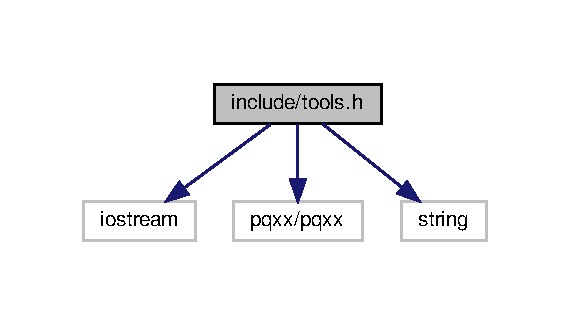
\includegraphics[width=274pt]{d5/dcd/tools_8h__incl}
\end{center}
\end{figure}
This graph shows which files directly or indirectly include this file\+:\nopagebreak
\begin{figure}[H]
\begin{center}
\leavevmode
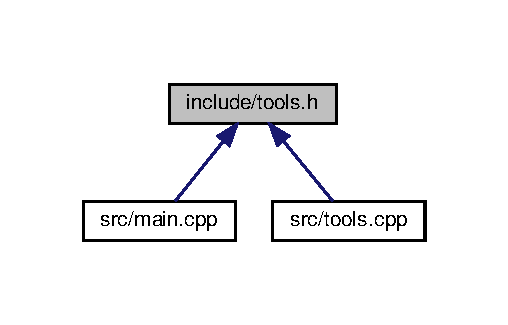
\includegraphics[width=244pt]{d6/ddf/tools_8h__dep__incl}
\end{center}
\end{figure}
\subsection*{Functions}
\begin{DoxyCompactItemize}
\item 
void \hyperlink{tools_8h_a61c5db3de2e3870f15756d0ad8440990}{error} (std\+::string str)
\begin{DoxyCompactList}\small\item\em error Display the passed string thne exit the program. \end{DoxyCompactList}\item 
void \hyperlink{tools_8h_a91602e2ffffd88f2b5f4280ef0d9e3be}{usage} (std\+::vector$<$ std\+::string $>$ \&optf, std\+::vector$<$ std\+::string $>$ \&optl, std\+::vector$<$ std\+::string $>$ \&optv)
\begin{DoxyCompactList}\small\item\em usage Display the usage, then exit the program. \end{DoxyCompactList}\item 
void \hyperlink{tools_8h_afc65291b27e568d76cf11518d7c2123e}{get\+\_\+arg} (int argc, char $\ast$$\ast$argv, std\+::vector$<$ std\+::string $>$ \&optf, std\+::vector$<$ std\+::string $>$ \&optl, std\+::vector$<$ std\+::string $>$ \&optv)
\begin{DoxyCompactList}\small\item\em get\+\_\+arg Search for the potential argument in the argument passed to the program. \end{DoxyCompactList}\end{DoxyCompactItemize}


\subsection{Function Documentation}
\mbox{\Hypertarget{tools_8h_a61c5db3de2e3870f15756d0ad8440990}\label{tools_8h_a61c5db3de2e3870f15756d0ad8440990}} 
\index{tools.\+h@{tools.\+h}!error@{error}}
\index{error@{error}!tools.\+h@{tools.\+h}}
\subsubsection{\texorpdfstring{error()}{error()}}
{\footnotesize\ttfamily void error (\begin{DoxyParamCaption}\item[{std\+::string}]{str }\end{DoxyParamCaption})}



error Display the passed string thne exit the program. 


\begin{DoxyParams}{Parameters}
{\em str} & String to display. \\
\hline
\end{DoxyParams}
\mbox{\Hypertarget{tools_8h_afc65291b27e568d76cf11518d7c2123e}\label{tools_8h_afc65291b27e568d76cf11518d7c2123e}} 
\index{tools.\+h@{tools.\+h}!get\+\_\+arg@{get\+\_\+arg}}
\index{get\+\_\+arg@{get\+\_\+arg}!tools.\+h@{tools.\+h}}
\subsubsection{\texorpdfstring{get\+\_\+arg()}{get\_arg()}}
{\footnotesize\ttfamily void get\+\_\+arg (\begin{DoxyParamCaption}\item[{int}]{argc,  }\item[{char $\ast$$\ast$}]{argv,  }\item[{std\+::vector$<$ std\+::string $>$ \&}]{optf,  }\item[{std\+::vector$<$ std\+::string $>$ \&}]{optl,  }\item[{std\+::vector$<$ std\+::string $>$ \&}]{optv }\end{DoxyParamCaption})}



get\+\_\+arg Search for the potential argument in the argument passed to the program. 


\begin{DoxyParams}{Parameters}
{\em argc} & Argument counter \\
\hline
{\em argv} & Argument array \\
\hline
{\em optf} & List of option flags \\
\hline
{\em optf} & List of option labels \\
\hline
{\em optf} & List of option values \\
\hline
\end{DoxyParams}
\mbox{\Hypertarget{tools_8h_a91602e2ffffd88f2b5f4280ef0d9e3be}\label{tools_8h_a91602e2ffffd88f2b5f4280ef0d9e3be}} 
\index{tools.\+h@{tools.\+h}!usage@{usage}}
\index{usage@{usage}!tools.\+h@{tools.\+h}}
\subsubsection{\texorpdfstring{usage()}{usage()}}
{\footnotesize\ttfamily void usage (\begin{DoxyParamCaption}\item[{std\+::vector$<$ std\+::string $>$ \&}]{optf,  }\item[{std\+::vector$<$ std\+::string $>$ \&}]{optl,  }\item[{std\+::vector$<$ std\+::string $>$ \&}]{optv }\end{DoxyParamCaption})}



usage Display the usage, then exit the program. 


\begin{DoxyParams}{Parameters}
{\em optf} & List of option flags \\
\hline
{\em optf} & List of option labels \\
\hline
{\em optf} & List of option values \\
\hline
\end{DoxyParams}

\hypertarget{moc__mainwindow_8cpp}{}\section{O\+T\+Bconfig\+G\+U\+I/build/moc\+\_\+mainwindow.cpp File Reference}
\label{moc__mainwindow_8cpp}\index{O\+T\+Bconfig\+G\+U\+I/build/moc\+\_\+mainwindow.\+cpp@{O\+T\+Bconfig\+G\+U\+I/build/moc\+\_\+mainwindow.\+cpp}}
{\ttfamily \#include \char`\"{}../include/mainwindow.\+h\char`\"{}}\newline
{\ttfamily \#include $<$Qt\+Core/qbytearray.\+h$>$}\newline
{\ttfamily \#include $<$Qt\+Core/qmetatype.\+h$>$}\newline
Include dependency graph for moc\+\_\+mainwindow.\+cpp\+:
\nopagebreak
\begin{figure}[H]
\begin{center}
\leavevmode
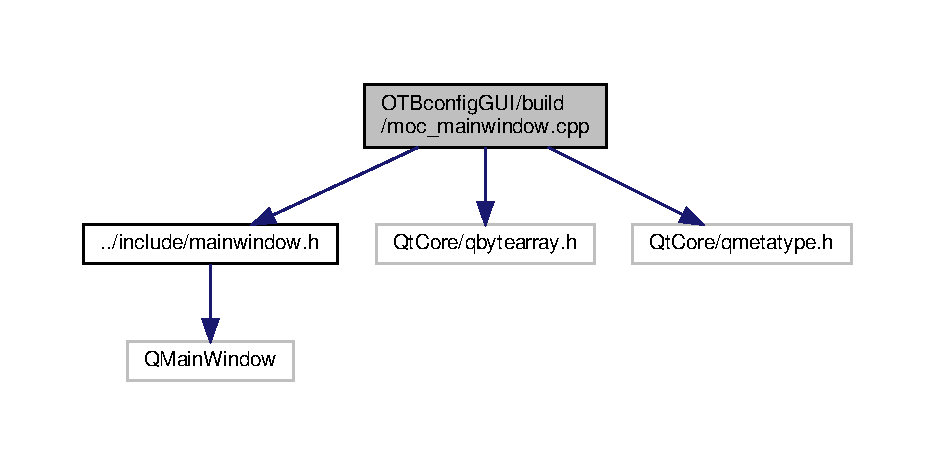
\includegraphics[width=350pt]{d6/d2a/moc__mainwindow_8cpp__incl}
\end{center}
\end{figure}
\subsection*{Classes}
\begin{DoxyCompactItemize}
\item 
struct \hyperlink{structqt__meta__stringdata___main_window__t}{qt\+\_\+meta\+\_\+stringdata\+\_\+\+Main\+Window\+\_\+t}
\end{DoxyCompactItemize}
\subsection*{Macros}
\begin{DoxyCompactItemize}
\item 
\#define \hyperlink{moc__mainwindow_8cpp_a75bb9482d242cde0a06c9dbdc6b83abe}{Q\+T\+\_\+\+M\+O\+C\+\_\+\+L\+I\+T\+E\+R\+AL}(idx,  ofs,  len)
\end{DoxyCompactItemize}


\subsection{Macro Definition Documentation}
\mbox{\Hypertarget{moc__mainwindow_8cpp_a75bb9482d242cde0a06c9dbdc6b83abe}\label{moc__mainwindow_8cpp_a75bb9482d242cde0a06c9dbdc6b83abe}} 
\index{moc\+\_\+mainwindow.\+cpp@{moc\+\_\+mainwindow.\+cpp}!Q\+T\+\_\+\+M\+O\+C\+\_\+\+L\+I\+T\+E\+R\+AL@{Q\+T\+\_\+\+M\+O\+C\+\_\+\+L\+I\+T\+E\+R\+AL}}
\index{Q\+T\+\_\+\+M\+O\+C\+\_\+\+L\+I\+T\+E\+R\+AL@{Q\+T\+\_\+\+M\+O\+C\+\_\+\+L\+I\+T\+E\+R\+AL}!moc\+\_\+mainwindow.\+cpp@{moc\+\_\+mainwindow.\+cpp}}
\subsubsection{\texorpdfstring{Q\+T\+\_\+\+M\+O\+C\+\_\+\+L\+I\+T\+E\+R\+AL}{QT\_MOC\_LITERAL}}
{\footnotesize\ttfamily \#define Q\+T\+\_\+\+M\+O\+C\+\_\+\+L\+I\+T\+E\+R\+AL(\begin{DoxyParamCaption}\item[{}]{idx,  }\item[{}]{ofs,  }\item[{}]{len }\end{DoxyParamCaption})}

{\bfseries Value\+:}
\begin{DoxyCode}
Q\_STATIC\_BYTE\_ARRAY\_DATA\_HEADER\_INITIALIZER\_WITH\_OFFSET(len, \(\backslash\)
    qptrdiff(offsetof(\hyperlink{structqt__meta__stringdata___main_window__t}{qt\_meta\_stringdata\_MainWindow\_t}, stringdata0) + ofs \(\backslash\)
        - idx * \textcolor{keyword}{sizeof}(QByteArrayData)) \(\backslash\)
    )
\end{DoxyCode}

\hypertarget{moc__predefs_8h}{}\section{O\+T\+Bconfig\+G\+U\+I/build/moc\+\_\+predefs.h File Reference}
\label{moc__predefs_8h}\index{O\+T\+Bconfig\+G\+U\+I/build/moc\+\_\+predefs.\+h@{O\+T\+Bconfig\+G\+U\+I/build/moc\+\_\+predefs.\+h}}
\subsection*{Macros}
\begin{DoxyCompactItemize}
\item 
\#define \hyperlink{moc__predefs_8h_ac7368721a5741c75d58bc978c47bf1df}{\+\_\+\+\_\+\+S\+S\+P\+\_\+\+S\+T\+R\+O\+N\+G\+\_\+\+\_\+}~3
\item 
\#define \hyperlink{moc__predefs_8h_a63d6f5d1c3371192fe03b3fb06e82400}{\+\_\+\+\_\+\+D\+B\+L\+\_\+\+M\+I\+N\+\_\+\+E\+X\+P\+\_\+\+\_\+}~(-\/1021)
\item 
\#define \hyperlink{moc__predefs_8h_a6605c8368985e3b1885a84d1d44ff798}{\+\_\+\+\_\+\+F\+L\+T32\+X\+\_\+\+M\+A\+X\+\_\+\+E\+X\+P\+\_\+\+\_\+}~1024
\item 
\#define \hyperlink{moc__predefs_8h_ac47e77d27e7d30f01cde452a9cd218ed}{\+\_\+\+\_\+cpp\+\_\+attributes}~200809
\item 
\#define \hyperlink{moc__predefs_8h_a6a762b969d5eea9e6a8db715a5f5a1a9}{\+\_\+\+\_\+\+U\+I\+N\+T\+\_\+\+L\+E\+A\+S\+T16\+\_\+\+M\+A\+X\+\_\+\+\_\+}~0xffff
\item 
\#define \hyperlink{moc__predefs_8h_a72e3c30a05bd2bb63d76550e451a438e}{\+\_\+\+\_\+\+A\+T\+O\+M\+I\+C\+\_\+\+A\+C\+Q\+U\+I\+RE}~2
\item 
\#define \hyperlink{moc__predefs_8h_af071b48310b9018035302c28cfd0424e}{\+\_\+\+\_\+\+F\+L\+T128\+\_\+\+M\+A\+X\+\_\+10\+\_\+\+E\+X\+P\+\_\+\+\_\+}~4932
\item 
\#define \hyperlink{moc__predefs_8h_a6e947aa0a2cb4808d560339fef0d4793}{\+\_\+\+\_\+\+F\+L\+T\+\_\+\+M\+I\+N\+\_\+\+\_\+}~1.\+17549435082228750796873653722224568e-\/38F
\item 
\#define \hyperlink{moc__predefs_8h_a779a207685ad2b8ca4cdab02ece517eb}{\+\_\+\+\_\+\+G\+C\+C\+\_\+\+I\+E\+C\+\_\+559\+\_\+\+C\+O\+M\+P\+L\+EX}~2
\item 
\#define \hyperlink{moc__predefs_8h_a5a8c0a31337df765b55c6260ef58e51e}{\+\_\+\+\_\+\+U\+I\+N\+T\+\_\+\+L\+E\+A\+S\+T8\+\_\+\+T\+Y\+P\+E\+\_\+\+\_\+}~unsigned char
\item 
\#define \hyperlink{moc__predefs_8h_acb072d4167167be73828de722a2def0b}{\+\_\+\+\_\+\+S\+I\+Z\+E\+O\+F\+\_\+\+F\+L\+O\+A\+T80\+\_\+\+\_\+}~16
\item 
\#define \hyperlink{moc__predefs_8h_adb0d09cff489746c5456407aa832fced}{\+\_\+\+\_\+\+I\+N\+T\+M\+A\+X\+\_\+C}(c)~c \#\# L
\item 
\#define \hyperlink{moc__predefs_8h_ab35e271dce6e7e2190d60b5905375419}{\+\_\+\+\_\+\+C\+H\+A\+R\+\_\+\+B\+I\+T\+\_\+\+\_\+}~8
\item 
\#define \hyperlink{moc__predefs_8h_afd12ac7489bdbbed7fa3cc51023b8f73}{\+\_\+\+\_\+\+U\+I\+N\+T8\+\_\+\+M\+A\+X\+\_\+\+\_\+}~0xff
\item 
\#define \hyperlink{moc__predefs_8h_a8925e15bce319fa2f42c659f6a3e0199}{\+\_\+\+\_\+\+W\+I\+N\+T\+\_\+\+M\+A\+X\+\_\+\+\_\+}~0xffffffffU
\item 
\#define \hyperlink{moc__predefs_8h_a300c6970bb64b04e45a9c2ed139ecce8}{\+\_\+\+\_\+\+F\+L\+T32\+\_\+\+M\+I\+N\+\_\+\+E\+X\+P\+\_\+\+\_\+}~(-\/125)
\item 
\#define \hyperlink{moc__predefs_8h_a60c56e472a1144b03053a2c7a2abb7fb}{\+\_\+\+\_\+cpp\+\_\+static\+\_\+assert}~200410
\item 
\#define \hyperlink{moc__predefs_8h_a2b695357ce4b46971d54e8e9dfe5724f}{\+\_\+\+\_\+\+O\+R\+D\+E\+R\+\_\+\+L\+I\+T\+T\+L\+E\+\_\+\+E\+N\+D\+I\+A\+N\+\_\+\+\_\+}~1234
\item 
\#define \hyperlink{moc__predefs_8h_a66fbb70a69c9f66830f95a20e46091a6}{\+\_\+\+\_\+\+S\+I\+Z\+E\+\_\+\+M\+A\+X\+\_\+\+\_\+}~0xffffffffffffffff\+UL
\item 
\#define \hyperlink{moc__predefs_8h_a65ac8cd0434319a3a31dc031409c218a}{\+\_\+\+\_\+\+W\+C\+H\+A\+R\+\_\+\+M\+A\+X\+\_\+\+\_\+}~0x7fffffff
\item 
\#define \hyperlink{moc__predefs_8h_a33433eca9e18e14156165252746f4d44}{\+\_\+\+\_\+\+G\+C\+C\+\_\+\+H\+A\+V\+E\+\_\+\+S\+Y\+N\+C\+\_\+\+C\+O\+M\+P\+A\+R\+E\+\_\+\+A\+N\+D\+\_\+\+S\+W\+A\+P\+\_\+1}~1
\item 
\#define \hyperlink{moc__predefs_8h_a7237ce09defceeebe3ba0afc528275ac}{\+\_\+\+\_\+\+G\+C\+C\+\_\+\+H\+A\+V\+E\+\_\+\+S\+Y\+N\+C\+\_\+\+C\+O\+M\+P\+A\+R\+E\+\_\+\+A\+N\+D\+\_\+\+S\+W\+A\+P\+\_\+2}~1
\item 
\#define \hyperlink{moc__predefs_8h_a6310789290c9c5717826b56443ce69ec}{\+\_\+\+\_\+\+G\+C\+C\+\_\+\+H\+A\+V\+E\+\_\+\+S\+Y\+N\+C\+\_\+\+C\+O\+M\+P\+A\+R\+E\+\_\+\+A\+N\+D\+\_\+\+S\+W\+A\+P\+\_\+4}~1
\item 
\#define \hyperlink{moc__predefs_8h_aca2a716d3e84ccffe000390bb2e2fb38}{\+\_\+\+\_\+\+D\+B\+L\+\_\+\+D\+E\+N\+O\+R\+M\+\_\+\+M\+I\+N\+\_\+\+\_\+}~double(4.\+94065645841246544176568792868221372e-\/324\+L)
\item 
\#define \hyperlink{moc__predefs_8h_a86bb5059d696b19082c1aff4ae93a87a}{\+\_\+\+\_\+\+G\+C\+C\+\_\+\+H\+A\+V\+E\+\_\+\+S\+Y\+N\+C\+\_\+\+C\+O\+M\+P\+A\+R\+E\+\_\+\+A\+N\+D\+\_\+\+S\+W\+A\+P\+\_\+8}~1
\item 
\#define \hyperlink{moc__predefs_8h_a403ff8d656461ff5a083fb47f73c7da3}{\+\_\+\+\_\+\+G\+C\+C\+\_\+\+A\+T\+O\+M\+I\+C\+\_\+\+C\+H\+A\+R\+\_\+\+L\+O\+C\+K\+\_\+\+F\+R\+EE}~2
\item 
\#define \hyperlink{moc__predefs_8h_a0a3bd26d0b040f0781a238e4aedd3dbe}{\+\_\+\+\_\+\+G\+C\+C\+\_\+\+I\+E\+C\+\_\+559}~2
\item 
\#define \hyperlink{moc__predefs_8h_a00a9f6ceb42fbe18b789b4c1949c49f2}{\+\_\+\+\_\+\+F\+L\+T32\+X\+\_\+\+D\+E\+C\+I\+M\+A\+L\+\_\+\+D\+I\+G\+\_\+\+\_\+}~17
\item 
\#define \hyperlink{moc__predefs_8h_a737828904768e0ab49acbdb3371d8445}{\+\_\+\+\_\+\+F\+L\+T\+\_\+\+E\+V\+A\+L\+\_\+\+M\+E\+T\+H\+O\+D\+\_\+\+\_\+}~0
\item 
\#define \hyperlink{moc__predefs_8h_aa5be39d362c571d48d6236f0bd58f1fc}{\+\_\+\+\_\+unix\+\_\+\+\_\+}~1
\item 
\#define \hyperlink{moc__predefs_8h_ade9dc15e022182eb0a62a0fd17d18b75}{\+\_\+\+\_\+cpp\+\_\+binary\+\_\+literals}~201304
\item 
\#define \hyperlink{moc__predefs_8h_a8ef55ba782e9d01cb22911f97168d06a}{\+\_\+\+\_\+\+F\+L\+T64\+\_\+\+D\+E\+C\+I\+M\+A\+L\+\_\+\+D\+I\+G\+\_\+\+\_\+}~17
\item 
\#define \hyperlink{moc__predefs_8h_a98e298953067135caf4bc0b8e8e7cd01}{\+\_\+\+\_\+\+G\+C\+C\+\_\+\+A\+T\+O\+M\+I\+C\+\_\+\+C\+H\+A\+R32\+\_\+\+T\+\_\+\+L\+O\+C\+K\+\_\+\+F\+R\+EE}~2
\item 
\#define \hyperlink{moc__predefs_8h_a64b6ba77bbc2cb5db2a19f32e954fcc3}{\+\_\+\+\_\+x86\+\_\+64}~1
\item 
\#define \hyperlink{moc__predefs_8h_a559dd2b0792fc2b0b30ba1dd66ca7cdc}{\+\_\+\+\_\+cpp\+\_\+variadic\+\_\+templates}~200704
\item 
\#define \hyperlink{moc__predefs_8h_a17a1ff08595cf7e0c9d1f162b727ccb6}{\+\_\+\+\_\+\+U\+I\+N\+T\+\_\+\+F\+A\+S\+T64\+\_\+\+M\+A\+X\+\_\+\+\_\+}~0xffffffffffffffff\+UL
\item 
\#define \hyperlink{moc__predefs_8h_ac60fe3845f87fdaf6365a733ede87cfe}{\+\_\+\+\_\+\+S\+I\+G\+\_\+\+A\+T\+O\+M\+I\+C\+\_\+\+T\+Y\+P\+E\+\_\+\+\_\+}~int
\item 
\#define \hyperlink{moc__predefs_8h_a1abd7cf346a460459d7fe1a9d4b5dde9}{\+\_\+\+\_\+\+D\+B\+L\+\_\+\+M\+I\+N\+\_\+10\+\_\+\+E\+X\+P\+\_\+\+\_\+}~(-\/307)
\item 
\#define \hyperlink{moc__predefs_8h_a611d40c375b1972669292fd27bc4afb7}{\+\_\+\+\_\+\+F\+I\+N\+I\+T\+E\+\_\+\+M\+A\+T\+H\+\_\+\+O\+N\+L\+Y\+\_\+\+\_\+}~0
\item 
\#define \hyperlink{moc__predefs_8h_ad149c0565fcf669b23f483e5b7f80dbd}{\+\_\+\+\_\+\+G\+N\+U\+C\+\_\+\+P\+A\+T\+C\+H\+L\+E\+V\+E\+L\+\_\+\+\_\+}~0
\item 
\#define \hyperlink{moc__predefs_8h_ac1175c9478c586edee06d1f788a03b83}{\+\_\+\+\_\+\+F\+L\+T32\+\_\+\+H\+A\+S\+\_\+\+D\+E\+N\+O\+R\+M\+\_\+\+\_\+}~1
\item 
\#define \hyperlink{moc__predefs_8h_a27b5eb7cfda61c7f1baeb4d95f3052bb}{\+\_\+\+\_\+\+U\+I\+N\+T\+\_\+\+F\+A\+S\+T8\+\_\+\+M\+A\+X\+\_\+\+\_\+}~0xff
\item 
\#define \hyperlink{moc__predefs_8h_a1c6886956b05c16006d924f77a868410}{\+\_\+\+\_\+has\+\_\+include}(S\+TR)~\+\_\+\+\_\+has\+\_\+include\+\_\+\+\_\+(S\+TR)
\item 
\#define \hyperlink{moc__predefs_8h_a3d4fe0f0b2e3ae12569d4a663dee8a0c}{\+\_\+\+\_\+\+D\+E\+C64\+\_\+\+M\+A\+X\+\_\+\+E\+X\+P\+\_\+\+\_\+}~385
\item 
\#define \hyperlink{moc__predefs_8h_ad36bc14a0433c9f88496bed4ccbd65a3}{\+\_\+\+\_\+\+I\+N\+T8\+\_\+C}(c)~c
\item 
\#define \hyperlink{moc__predefs_8h_a967b4ada96d28b97bc07e26e1def8e66}{\+\_\+\+\_\+\+I\+N\+T\+\_\+\+L\+E\+A\+S\+T8\+\_\+\+W\+I\+D\+T\+H\+\_\+\+\_\+}~8
\item 
\#define \hyperlink{moc__predefs_8h_a4bf843ffcadf9b162b74c1b7e546e8e9}{\+\_\+\+\_\+\+U\+I\+N\+T\+\_\+\+L\+E\+A\+S\+T64\+\_\+\+M\+A\+X\+\_\+\+\_\+}~0xffffffffffffffff\+UL
\item 
\#define \hyperlink{moc__predefs_8h_a4f69990d03f9fb0c390a6fbad28a737b}{\+\_\+\+\_\+\+S\+H\+R\+T\+\_\+\+M\+A\+X\+\_\+\+\_\+}~0x7fff
\item 
\#define \hyperlink{moc__predefs_8h_a06fd91f0507a4f364e469c8055f4265a}{\+\_\+\+\_\+\+L\+D\+B\+L\+\_\+\+M\+A\+X\+\_\+\+\_\+}~1.\+18973149535723176502126385303097021e+4932L
\item 
\#define \hyperlink{moc__predefs_8h_af707469f32a983b229e6c7e0e4efc063}{\+\_\+\+\_\+\+F\+L\+T64\+X\+\_\+\+M\+A\+X\+\_\+10\+\_\+\+E\+X\+P\+\_\+\+\_\+}~4932
\item 
\#define \hyperlink{moc__predefs_8h_aaf06a1464d33431377a2ee5293ec70d2}{\+\_\+\+\_\+\+U\+I\+N\+T\+\_\+\+L\+E\+A\+S\+T8\+\_\+\+M\+A\+X\+\_\+\+\_\+}~0xff
\item 
\#define \hyperlink{moc__predefs_8h_a9685ff8e617f3c5892c2a6fe3484f3b7}{\+\_\+\+\_\+\+G\+C\+C\+\_\+\+A\+T\+O\+M\+I\+C\+\_\+\+B\+O\+O\+L\+\_\+\+L\+O\+C\+K\+\_\+\+F\+R\+EE}~2
\item 
\#define \hyperlink{moc__predefs_8h_a960cb27a87591af89eddb328647f1534}{\+\_\+\+\_\+\+F\+L\+T128\+\_\+\+D\+E\+N\+O\+R\+M\+\_\+\+M\+I\+N\+\_\+\+\_\+}~6.\+47517511943802511092443895822764655e-\/4966\+F128
\item 
\#define \hyperlink{moc__predefs_8h_ab86380373ae9fa385c8a2464023774a8}{\+\_\+\+\_\+\+U\+I\+N\+T\+M\+A\+X\+\_\+\+T\+Y\+P\+E\+\_\+\+\_\+}~long unsigned int
\item 
\#define \hyperlink{moc__predefs_8h_a6c6342c53a7213211680dc5caae14491}{\+\_\+\+\_\+linux}~1
\item 
\#define \hyperlink{moc__predefs_8h_a13526b223391d4982c4c172c29bfdc1e}{\+\_\+\+\_\+\+D\+E\+C32\+\_\+\+E\+P\+S\+I\+L\+O\+N\+\_\+\+\_\+}~1\+E-\/6\+DF
\item 
\#define \hyperlink{moc__predefs_8h_af635b5d104ef9858a68ab2c56677fd2d}{\+\_\+\+\_\+\+F\+L\+T\+\_\+\+E\+V\+A\+L\+\_\+\+M\+E\+T\+H\+O\+D\+\_\+\+T\+S\+\_\+18661\+\_\+3\+\_\+\+\_\+}~0
\item 
\#define \hyperlink{moc__predefs_8h_a5bcf2962d7a37c34484cef13fa9601b2}{\+\_\+\+\_\+\+O\+P\+T\+I\+M\+I\+Z\+E\+\_\+\+\_\+}~1
\item 
\#define \hyperlink{moc__predefs_8h_ac3cd8b035cfb8a68f6d1119ace36f1cc}{\+\_\+\+\_\+unix}~1
\item 
\#define \hyperlink{moc__predefs_8h_ab4425dccbcddb2363a2a8a67367a5b42}{\+\_\+\+\_\+\+U\+I\+N\+T32\+\_\+\+M\+A\+X\+\_\+\+\_\+}~0xffffffffU
\item 
\#define \hyperlink{moc__predefs_8h_a213133a8dca206becf88c2e3523b124a}{\+\_\+\+\_\+\+G\+X\+X\+\_\+\+E\+X\+P\+E\+R\+I\+M\+E\+N\+T\+A\+L\+\_\+\+C\+X\+X0\+X\+\_\+\+\_\+}~1
\item 
\#define \hyperlink{moc__predefs_8h_ae221a8e373285cf10c22926762f477f5}{\+\_\+\+\_\+\+L\+D\+B\+L\+\_\+\+M\+A\+X\+\_\+\+E\+X\+P\+\_\+\+\_\+}~16384
\item 
\#define \hyperlink{moc__predefs_8h_aad2e8f7e8d06ab966a1210f4a7d65770}{\+\_\+\+\_\+\+F\+L\+T128\+\_\+\+M\+I\+N\+\_\+\+E\+X\+P\+\_\+\+\_\+}~(-\/16381)
\item 
\#define \hyperlink{moc__predefs_8h_a135696718aa5b38e58be73aaece6654f}{\+\_\+\+\_\+\+W\+I\+N\+T\+\_\+\+M\+I\+N\+\_\+\+\_\+}~0U
\item 
\#define \hyperlink{moc__predefs_8h_a1b27e3508a4c1e97875297882a95f503}{\+\_\+\+\_\+linux\+\_\+\+\_\+}~1
\item 
\#define \hyperlink{moc__predefs_8h_a784d5a4b7494076d83772a819916b039}{\+\_\+\+\_\+\+F\+L\+T128\+\_\+\+M\+I\+N\+\_\+10\+\_\+\+E\+X\+P\+\_\+\+\_\+}~(-\/4931)
\item 
\#define \hyperlink{moc__predefs_8h_a6091ba87f9a538a9685b7997a64a64db}{\+\_\+\+\_\+\+I\+N\+T\+\_\+\+L\+E\+A\+S\+T16\+\_\+\+W\+I\+D\+T\+H\+\_\+\+\_\+}~16
\item 
\#define \hyperlink{moc__predefs_8h_a87b7ceac2198cab045e40c9a64b11679}{\+\_\+\+\_\+\+S\+C\+H\+A\+R\+\_\+\+M\+A\+X\+\_\+\+\_\+}~0x7f
\item 
\#define \hyperlink{moc__predefs_8h_a39e5016b6c2adbc3a6b1674c458d4dc5}{\+\_\+\+\_\+\+F\+L\+T128\+\_\+\+M\+A\+N\+T\+\_\+\+D\+I\+G\+\_\+\+\_\+}~113
\item 
\#define \hyperlink{moc__predefs_8h_a01b915d3ec5439de746f1d5e9f76dc3d}{\+\_\+\+\_\+\+W\+C\+H\+A\+R\+\_\+\+M\+I\+N\+\_\+\+\_\+}~(-\/\hyperlink{moc__predefs_8h_a65ac8cd0434319a3a31dc031409c218a}{\+\_\+\+\_\+\+W\+C\+H\+A\+R\+\_\+\+M\+A\+X\+\_\+\+\_\+} -\/ 1)
\item 
\#define \hyperlink{moc__predefs_8h_a4b8971e411b88166747d2a3c2425eaee}{\+\_\+\+\_\+\+I\+N\+T64\+\_\+C}(c)~c \#\# L
\item 
\#define \hyperlink{moc__predefs_8h_a61969667ef3b668024a20df9bc34c991}{\+\_\+\+\_\+\+D\+B\+L\+\_\+\+D\+I\+G\+\_\+\+\_\+}~15
\item 
\#define \hyperlink{moc__predefs_8h_aa808bc3159395526ac0c07d36b87dec1}{\+\_\+\+\_\+\+G\+C\+C\+\_\+\+A\+T\+O\+M\+I\+C\+\_\+\+P\+O\+I\+N\+T\+E\+R\+\_\+\+L\+O\+C\+K\+\_\+\+F\+R\+EE}~2
\item 
\#define \hyperlink{moc__predefs_8h_ac070fafc444399b9243e0366b4ce4ef7}{\+\_\+\+\_\+\+F\+L\+T64\+X\+\_\+\+M\+A\+N\+T\+\_\+\+D\+I\+G\+\_\+\+\_\+}~64
\item 
\#define \hyperlink{moc__predefs_8h_ac95d263a48eda25c373846eb54144fc4}{\+\_\+\+F\+O\+R\+T\+I\+F\+Y\+\_\+\+S\+O\+U\+R\+CE}~2
\item 
\#define \hyperlink{moc__predefs_8h_a4b2be09502f3fe1cd13838c6761803b3}{\+\_\+\+\_\+\+S\+I\+Z\+E\+O\+F\+\_\+\+I\+N\+T\+\_\+\+\_\+}~4
\item 
\#define \hyperlink{moc__predefs_8h_a8bd657ce95940b7c6087cf5aa54d5280}{\+\_\+\+\_\+\+S\+I\+Z\+E\+O\+F\+\_\+\+P\+O\+I\+N\+T\+E\+R\+\_\+\+\_\+}~8
\item 
\#define \hyperlink{moc__predefs_8h_a7f18358ae5a65523140cb561bbeaa3a9}{\+\_\+\+\_\+\+G\+C\+C\+\_\+\+A\+T\+O\+M\+I\+C\+\_\+\+C\+H\+A\+R16\+\_\+\+T\+\_\+\+L\+O\+C\+K\+\_\+\+F\+R\+EE}~2
\item 
\#define \hyperlink{moc__predefs_8h_aff6bf0ff0fa3b5cbd23a8ae1131c87a9}{\+\_\+\+\_\+\+U\+S\+E\+R\+\_\+\+L\+A\+B\+E\+L\+\_\+\+P\+R\+E\+F\+I\+X\+\_\+\+\_\+}
\item 
\#define \hyperlink{moc__predefs_8h_a098c7fe44eed71241990da5db8f99bc3}{\+\_\+\+\_\+\+F\+L\+T64\+X\+\_\+\+E\+P\+S\+I\+L\+O\+N\+\_\+\+\_\+}~1.\+08420217248550443400745280086994171e-\/19\+F64x
\item 
\#define \hyperlink{moc__predefs_8h_a309fa84aefd09132258bbe21c20ef7d4}{\+\_\+\+\_\+\+S\+T\+D\+C\+\_\+\+H\+O\+S\+T\+E\+D\+\_\+\+\_\+}~1
\item 
\#define \hyperlink{moc__predefs_8h_a87140cc80075e8907e7bbfd910c5642a}{\+\_\+\+\_\+\+L\+D\+B\+L\+\_\+\+H\+A\+S\+\_\+\+I\+N\+F\+I\+N\+I\+T\+Y\+\_\+\+\_\+}~1
\item 
\#define \hyperlink{moc__predefs_8h_aa021702c3b7627dccaa51c33a2c5a8d1}{\+\_\+\+\_\+\+F\+L\+T32\+\_\+\+D\+I\+G\+\_\+\+\_\+}~6
\item 
\#define \hyperlink{moc__predefs_8h_a7ac5a3b1dc00b508a391f8c6c37e2165}{\+\_\+\+\_\+\+F\+L\+T\+\_\+\+E\+P\+S\+I\+L\+O\+N\+\_\+\+\_\+}~1.\+19209289550781250000000000000000000e-\/7F
\item 
\#define \hyperlink{moc__predefs_8h_afb5a2a4891df4551832357e97c6c3c59}{\+\_\+\+\_\+\+G\+X\+X\+\_\+\+W\+E\+A\+K\+\_\+\+\_\+}~1
\item 
\#define \hyperlink{moc__predefs_8h_aeb2d8312284d49b1e44c7d003bd8b54b}{\+\_\+\+\_\+\+S\+H\+R\+T\+\_\+\+W\+I\+D\+T\+H\+\_\+\+\_\+}~16
\item 
\#define \hyperlink{moc__predefs_8h_ab572f59c4b0c5a1f4c2953f38a76d7b3}{\+\_\+\+\_\+\+L\+D\+B\+L\+\_\+\+M\+I\+N\+\_\+\+\_\+}~3.\+36210314311209350626267781732175260e-\/4932L
\item 
\#define \hyperlink{moc__predefs_8h_ad3165a97a460b88ccdea80967918f250}{\+\_\+\+\_\+\+D\+E\+C32\+\_\+\+M\+A\+X\+\_\+\+\_\+}~9.\+999999\+E96\+DF
\item 
\#define \hyperlink{moc__predefs_8h_aaa322b38474911c60e45134194bd6e8f}{\+\_\+\+\_\+cpp\+\_\+threadsafe\+\_\+static\+\_\+init}~200806
\item 
\#define \hyperlink{moc__predefs_8h_ac0fe3e739d0b847c07dde20eabf2ab3d}{\+\_\+\+\_\+\+F\+L\+T64\+X\+\_\+\+D\+E\+N\+O\+R\+M\+\_\+\+M\+I\+N\+\_\+\+\_\+}~3.\+64519953188247460252840593361941982e-\/4951\+F64x
\item 
\#define \hyperlink{moc__predefs_8h_a8f246ad899706f78b8dfcd33daff7b07}{\+\_\+\+\_\+\+F\+L\+T32\+X\+\_\+\+H\+A\+S\+\_\+\+I\+N\+F\+I\+N\+I\+T\+Y\+\_\+\+\_\+}~1
\item 
\#define \hyperlink{moc__predefs_8h_abf681096fa9e21512a3fe83f0dcfdb36}{\+\_\+\+\_\+\+I\+N\+T32\+\_\+\+M\+A\+X\+\_\+\+\_\+}~0x7fffffff
\item 
\#define \hyperlink{moc__predefs_8h_ad3907b8d9bb2265255e6e0d66d91d165}{\+\_\+\+\_\+\+I\+N\+T\+\_\+\+W\+I\+D\+T\+H\+\_\+\+\_\+}~32
\item 
\#define \hyperlink{moc__predefs_8h_aaa8084a56e3732008acafea8fd15eb2f}{\+\_\+\+\_\+\+S\+I\+Z\+E\+O\+F\+\_\+\+L\+O\+N\+G\+\_\+\+\_\+}~8
\item 
\#define \hyperlink{moc__predefs_8h_ab7d84ba8d87b8bb40aa752334bb51b23}{\+\_\+\+\_\+\+S\+T\+D\+C\+\_\+\+I\+E\+C\+\_\+559\+\_\+\+\_\+}~1
\item 
\#define \hyperlink{moc__predefs_8h_acb6063ed9d8841cf71c93f2bf34832e0}{\+\_\+\+\_\+\+S\+T\+D\+C\+\_\+\+I\+S\+O\+\_\+10646\+\_\+\+\_\+}~201706L
\item 
\#define \hyperlink{moc__predefs_8h_aa860a111dcff819d3502dda14f8ac778}{\+\_\+\+\_\+\+U\+I\+N\+T16\+\_\+C}(c)~c
\item 
\#define \hyperlink{moc__predefs_8h_a96b511bfa61e4203ec3668fb39063309}{\+\_\+\+\_\+\+P\+T\+R\+D\+I\+F\+F\+\_\+\+W\+I\+D\+T\+H\+\_\+\+\_\+}~64
\item 
\#define \hyperlink{moc__predefs_8h_aeb56455e98000942147dfd63ec1c2fa6}{\+\_\+\+\_\+\+D\+E\+C\+I\+M\+A\+L\+\_\+\+D\+I\+G\+\_\+\+\_\+}~21
\item 
\#define \hyperlink{moc__predefs_8h_ad293ff29c0ac9a6b4187d366d6de3772}{\+\_\+\+\_\+\+F\+L\+T64\+\_\+\+E\+P\+S\+I\+L\+O\+N\+\_\+\+\_\+}~2.\+22044604925031308084726333618164062e-\/16\+F64
\item 
\#define \hyperlink{moc__predefs_8h_a51b087854dc3c2f76946efb432745639}{\+\_\+\+\_\+gnu\+\_\+linux\+\_\+\+\_\+}~1
\item 
\#define \hyperlink{moc__predefs_8h_a4e8a5398566f8b2666a8a71b2dbcf3ca}{\+\_\+\+\_\+\+I\+N\+T\+M\+A\+X\+\_\+\+W\+I\+D\+T\+H\+\_\+\+\_\+}~64
\item 
\#define \hyperlink{moc__predefs_8h_aceda5e62622b9783846d26610d038f71}{\+\_\+\+\_\+\+F\+L\+T64\+\_\+\+M\+I\+N\+\_\+\+E\+X\+P\+\_\+\+\_\+}~(-\/1021)
\item 
\#define \hyperlink{moc__predefs_8h_a370369ba2463363de726ff9394861a2b}{\+\_\+\+\_\+has\+\_\+include\+\_\+next}(S\+TR)~\+\_\+\+\_\+has\+\_\+include\+\_\+next\+\_\+\+\_\+(S\+TR)
\item 
\#define \hyperlink{moc__predefs_8h_ad2396317be1036fdc4481d54343487de}{\+\_\+\+\_\+\+F\+L\+T64\+X\+\_\+\+M\+I\+N\+\_\+10\+\_\+\+E\+X\+P\+\_\+\+\_\+}~(-\/4931)
\item 
\#define \hyperlink{moc__predefs_8h_a10a15ae17c3b791fe9b9721965ebfee4}{\+\_\+\+\_\+\+L\+D\+B\+L\+\_\+\+H\+A\+S\+\_\+\+Q\+U\+I\+E\+T\+\_\+\+N\+A\+N\+\_\+\+\_\+}~1
\item 
\#define \hyperlink{moc__predefs_8h_a6c163c6e58545740cbae55ad8ffa027f}{\+\_\+\+\_\+\+F\+L\+T64\+\_\+\+M\+A\+N\+T\+\_\+\+D\+I\+G\+\_\+\+\_\+}~53
\item 
\#define \hyperlink{moc__predefs_8h_aa51016843ec55a0a9df7ce9f85767ee7}{\+\_\+\+\_\+\+G\+N\+U\+C\+\_\+\+\_\+}~7
\item 
\#define \hyperlink{moc__predefs_8h_af607715c8c9a98aa72c81c6629554b0d}{\+\_\+\+\_\+\+G\+X\+X\+\_\+\+R\+T\+TI}~1
\item 
\#define \hyperlink{moc__predefs_8h_a4b376612fb6ea83330a589449279da42}{\+\_\+\+\_\+pie\+\_\+\+\_\+}~2
\item 
\#define \hyperlink{moc__predefs_8h_ab61dd6e368adb90e2eff5739188b0bcb}{\+\_\+\+\_\+\+M\+M\+X\+\_\+\+\_\+}~1
\item 
\#define \hyperlink{moc__predefs_8h_a9e077def8c310cdb5fef37666a92c5a5}{\+\_\+\+\_\+cpp\+\_\+delegating\+\_\+constructors}~200604
\item 
\#define \hyperlink{moc__predefs_8h_a82a2c3ff271d1685b450975ffa68544a}{\+\_\+\+\_\+\+F\+L\+T\+\_\+\+H\+A\+S\+\_\+\+D\+E\+N\+O\+R\+M\+\_\+\+\_\+}~1
\item 
\#define \hyperlink{moc__predefs_8h_aae92712264b830cd7d24d4b81d502ffb}{\+\_\+\+\_\+\+S\+I\+Z\+E\+O\+F\+\_\+\+L\+O\+N\+G\+\_\+\+D\+O\+U\+B\+L\+E\+\_\+\+\_\+}~16
\item 
\#define \hyperlink{moc__predefs_8h_a2c25ec0f0ae74f9d8a7c373288a28dd1}{\+\_\+\+\_\+\+B\+I\+G\+G\+E\+S\+T\+\_\+\+A\+L\+I\+G\+N\+M\+E\+N\+T\+\_\+\+\_\+}~16
\item 
\#define \hyperlink{moc__predefs_8h_a93a5a9d251e5bff3c2a130627f20e782}{\+\_\+\+\_\+\+S\+T\+D\+C\+\_\+\+U\+T\+F\+\_\+16\+\_\+\+\_\+}~1
\item 
\#define \hyperlink{moc__predefs_8h_aeb14f5cf7cca3a01c2f6a0015e981eb1}{\+\_\+\+\_\+\+F\+L\+T64\+\_\+\+M\+A\+X\+\_\+10\+\_\+\+E\+X\+P\+\_\+\+\_\+}~308
\item 
\#define \hyperlink{moc__predefs_8h_a170219070ed7bdfea9f88121c9abbaea}{\+\_\+\+\_\+\+F\+L\+T32\+\_\+\+H\+A\+S\+\_\+\+I\+N\+F\+I\+N\+I\+T\+Y\+\_\+\+\_\+}~1
\item 
\#define \hyperlink{moc__predefs_8h_a711d7b7f27671b10b11a74c37f653ad7}{\+\_\+\+\_\+\+D\+B\+L\+\_\+\+M\+A\+X\+\_\+\+\_\+}~double(1.\+79769313486231570814527423731704357e+308\+L)
\item 
\#define \hyperlink{moc__predefs_8h_a7377e1bc6bd2fd9bcfe98283ab0e9037}{\+\_\+\+\_\+cpp\+\_\+raw\+\_\+strings}~200710
\item 
\#define \hyperlink{moc__predefs_8h_a84479d2bbe1d7286f406fcc302f41376}{\+\_\+\+\_\+\+I\+N\+T\+\_\+\+F\+A\+S\+T32\+\_\+\+M\+A\+X\+\_\+\+\_\+}~0x7fffffffffffffffL
\item 
\#define \hyperlink{moc__predefs_8h_a3dd03066dbb351dfa51353c80a7902a2}{\+\_\+\+\_\+\+D\+B\+L\+\_\+\+H\+A\+S\+\_\+\+I\+N\+F\+I\+N\+I\+T\+Y\+\_\+\+\_\+}~1
\item 
\#define \hyperlink{moc__predefs_8h_aa3f186f612efe5edfcc371c95617f06f}{\+\_\+\+\_\+\+I\+N\+T64\+\_\+\+M\+A\+X\+\_\+\+\_\+}~0x7fffffffffffffffL
\item 
\#define \hyperlink{moc__predefs_8h_a79e289c54a8c9851b2b118d442bbc26c}{\+\_\+\+\_\+\+D\+E\+C32\+\_\+\+M\+I\+N\+\_\+\+E\+X\+P\+\_\+\+\_\+}~(-\/94)
\item 
\#define \hyperlink{moc__predefs_8h_a8394afe92148ddbdf0e0697978cd1382}{\+\_\+\+\_\+\+I\+N\+T\+P\+T\+R\+\_\+\+W\+I\+D\+T\+H\+\_\+\+\_\+}~64
\item 
\#define \hyperlink{moc__predefs_8h_a97163404b3b71f857e35be74607f88f7}{\+\_\+\+\_\+\+F\+L\+T32\+X\+\_\+\+H\+A\+S\+\_\+\+D\+E\+N\+O\+R\+M\+\_\+\+\_\+}~1
\item 
\#define \hyperlink{moc__predefs_8h_a6a4d11835d03027f3929b84fe7b55bf6}{\+\_\+\+\_\+\+I\+N\+T\+\_\+\+F\+A\+S\+T16\+\_\+\+T\+Y\+P\+E\+\_\+\+\_\+}~long int
\item 
\#define \hyperlink{moc__predefs_8h_a3c7f3130e367d47bcc27a0a41278155e}{\+\_\+\+\_\+\+L\+D\+B\+L\+\_\+\+H\+A\+S\+\_\+\+D\+E\+N\+O\+R\+M\+\_\+\+\_\+}~1
\item 
\#define \hyperlink{moc__predefs_8h_a1b391bc7ed92f79666c4a5d840aa1edd}{\+\_\+\+\_\+cplusplus}~201103L
\item 
\#define \hyperlink{moc__predefs_8h_af73192acc2dd2095bd3524ca5ee9dca9}{\+\_\+\+\_\+cpp\+\_\+ref\+\_\+qualifiers}~200710
\item 
\#define \hyperlink{moc__predefs_8h_aaab7817ee2e4bb88b5178e101e7ab2a6}{\+\_\+\+\_\+\+D\+E\+C128\+\_\+\+M\+A\+X\+\_\+\+\_\+}~9.\+999999999999999999999999999999999\+E6144\+DL
\item 
\#define \hyperlink{moc__predefs_8h_a97e13c059a63d2d547cc4a9f386641d2}{\+\_\+\+\_\+\+I\+N\+T\+\_\+\+L\+E\+A\+S\+T32\+\_\+\+M\+A\+X\+\_\+\+\_\+}~0x7fffffff
\item 
\#define \hyperlink{moc__predefs_8h_a1f993b902b5b1dba7d5b043d0abc347b}{\+\_\+\+\_\+\+D\+E\+C32\+\_\+\+M\+I\+N\+\_\+\+\_\+}~1\+E-\/95\+DF
\item 
\#define \hyperlink{moc__predefs_8h_aa806e8f7ce2a8db3bf676735fca2ac51}{\+\_\+\+\_\+\+D\+E\+P\+R\+E\+C\+A\+T\+ED}~1
\item 
\#define \hyperlink{moc__predefs_8h_acfffb302850fa081bd63c30573077004}{\+\_\+\+\_\+cpp\+\_\+rvalue\+\_\+references}~200610
\item 
\#define \hyperlink{moc__predefs_8h_a9a8a7cd9484baf4b72ab15682745d119}{\+\_\+\+\_\+\+D\+B\+L\+\_\+\+M\+A\+X\+\_\+\+E\+X\+P\+\_\+\+\_\+}~1024
\item 
\#define \hyperlink{moc__predefs_8h_aba008af276ac0e3f85d1479af98f62b0}{\+\_\+\+\_\+\+W\+C\+H\+A\+R\+\_\+\+W\+I\+D\+T\+H\+\_\+\+\_\+}~32
\item 
\#define \hyperlink{moc__predefs_8h_a8d44614ef6d7f2bbbd9224d416d867b9}{\+\_\+\+\_\+\+F\+L\+T32\+\_\+\+M\+A\+X\+\_\+\+\_\+}~3.\+40282346638528859811704183484516925e+38\+F32
\item 
\#define \hyperlink{moc__predefs_8h_abd2230e0e187a5bae549a0ba786b311b}{\+\_\+\+\_\+\+D\+E\+C128\+\_\+\+E\+P\+S\+I\+L\+O\+N\+\_\+\+\_\+}~1\+E-\/33\+DL
\item 
\#define \hyperlink{moc__predefs_8h_ad8885a68f76fac734a20349f9b8cac69}{\+\_\+\+\_\+\+S\+S\+E2\+\_\+\+M\+A\+T\+H\+\_\+\+\_\+}~1
\item 
\#define \hyperlink{moc__predefs_8h_a6bb8315e719b7306f47cde3b4b30d91f}{\+\_\+\+\_\+\+A\+T\+O\+M\+I\+C\+\_\+\+H\+L\+E\+\_\+\+R\+E\+L\+E\+A\+SE}~131072
\item 
\#define \hyperlink{moc__predefs_8h_ac29c76a6702808cfc4a5f661d0d33c2c}{\+\_\+\+\_\+\+P\+T\+R\+D\+I\+F\+F\+\_\+\+M\+A\+X\+\_\+\+\_\+}~0x7fffffffffffffffL
\item 
\#define \hyperlink{moc__predefs_8h_ac78e83c300ae463c501bbe70c5a2a8c7}{\+\_\+\+\_\+amd64}~1
\item 
\#define \hyperlink{moc__predefs_8h_a80dc30fae2c51e5db5b4f5eb7400cd1a}{\+\_\+\+\_\+\+S\+T\+D\+C\+\_\+\+N\+O\+\_\+\+T\+H\+R\+E\+A\+D\+S\+\_\+\+\_\+}~1
\item 
\#define \hyperlink{moc__predefs_8h_ac227f24525ec0825a758b2eb0869dc8f}{\+\_\+\+\_\+\+A\+T\+O\+M\+I\+C\+\_\+\+H\+L\+E\+\_\+\+A\+C\+Q\+U\+I\+RE}~65536
\item 
\#define \hyperlink{moc__predefs_8h_a22791bdfea523b20c18eff848609fa9d}{\+\_\+\+\_\+\+F\+L\+T32\+\_\+\+H\+A\+S\+\_\+\+Q\+U\+I\+E\+T\+\_\+\+N\+A\+N\+\_\+\+\_\+}~1
\item 
\#define \hyperlink{moc__predefs_8h_ae7afb460abc6122c6a5f206d78bcae4e}{\+\_\+\+\_\+\+G\+N\+U\+G\+\_\+\+\_\+}~7
\item 
\#define \hyperlink{moc__predefs_8h_a9bed0d0b1893211f857ad76d6728ea7e}{\+\_\+\+\_\+\+L\+O\+N\+G\+\_\+\+L\+O\+N\+G\+\_\+\+M\+A\+X\+\_\+\+\_\+}~0x7fffffffffffffff\+LL
\item 
\#define \hyperlink{moc__predefs_8h_ab6eb3d66486ef05ac7f1d489bfc675b4}{\+\_\+\+\_\+\+S\+I\+Z\+E\+O\+F\+\_\+\+S\+I\+Z\+E\+\_\+\+T\+\_\+\+\_\+}~8
\item 
\#define \hyperlink{moc__predefs_8h_a6e4065bb57fe77e1d8635f8108bf3c64}{\+\_\+\+\_\+cpp\+\_\+rvalue\+\_\+reference}~200610
\item 
\#define \hyperlink{moc__predefs_8h_adeecd09fc579ff3f8222cf8ae581b936}{\+\_\+\+\_\+cpp\+\_\+nsdmi}~200809
\item 
\#define \hyperlink{moc__predefs_8h_a287cbae3fb7eb2bdc8906729897524c9}{\+\_\+\+\_\+\+F\+L\+T64\+X\+\_\+\+M\+I\+N\+\_\+\+E\+X\+P\+\_\+\+\_\+}~(-\/16381)
\item 
\#define \hyperlink{moc__predefs_8h_a808f04c28bb0ef2d6b77dd66564ad351}{\+\_\+\+\_\+\+S\+I\+Z\+E\+O\+F\+\_\+\+W\+I\+N\+T\+\_\+\+T\+\_\+\+\_\+}~4
\item 
\#define \hyperlink{moc__predefs_8h_a895181efde95bdfb3489ba3018c48582}{\+\_\+\+\_\+\+L\+O\+N\+G\+\_\+\+L\+O\+N\+G\+\_\+\+W\+I\+D\+T\+H\+\_\+\+\_\+}~64
\item 
\#define \hyperlink{moc__predefs_8h_a2b46de6050feed05210bef65feef9c42}{\+\_\+\+\_\+cpp\+\_\+initializer\+\_\+lists}~200806
\item 
\#define \hyperlink{moc__predefs_8h_a731bd57ce12918b6118b6a3e37c20d8e}{\+\_\+\+\_\+\+F\+L\+T32\+\_\+\+M\+A\+X\+\_\+\+E\+X\+P\+\_\+\+\_\+}~128
\item 
\#define \hyperlink{moc__predefs_8h_a0958474253d23ca2c87e817c16f74eda}{\+\_\+\+\_\+cpp\+\_\+hex\+\_\+float}~201603
\item 
\#define \hyperlink{moc__predefs_8h_a89cfc45cff96747b74ae03bdb2310814}{\+\_\+\+\_\+\+G\+C\+C\+\_\+\+H\+A\+V\+E\+\_\+\+D\+W\+A\+R\+F2\+\_\+\+C\+F\+I\+\_\+\+A\+SM}~1
\item 
\#define \hyperlink{moc__predefs_8h_aee5d0901405056d87e3bd47fee83128d}{\+\_\+\+\_\+\+G\+X\+X\+\_\+\+A\+B\+I\+\_\+\+V\+E\+R\+S\+I\+ON}~1011
\item 
\#define \hyperlink{moc__predefs_8h_a01763e0801406de2e88b94f4ad1298de}{\+\_\+\+\_\+\+F\+L\+T128\+\_\+\+H\+A\+S\+\_\+\+I\+N\+F\+I\+N\+I\+T\+Y\+\_\+\+\_\+}~1
\item 
\#define \hyperlink{moc__predefs_8h_acd7b9de9b6bd817027cb37ec6c82cba9}{\+\_\+\+\_\+\+F\+L\+T\+\_\+\+M\+I\+N\+\_\+\+E\+X\+P\+\_\+\+\_\+}~(-\/125)
\item 
\#define \hyperlink{moc__predefs_8h_a5eeda02831b3d7147a1a90f2d52a6228}{\+\_\+\+\_\+cpp\+\_\+lambdas}~200907
\item 
\#define \hyperlink{moc__predefs_8h_a5cef009cb95e257c235cd3e953bae15f}{\+\_\+\+\_\+\+F\+L\+T64\+X\+\_\+\+H\+A\+S\+\_\+\+Q\+U\+I\+E\+T\+\_\+\+N\+A\+N\+\_\+\+\_\+}~1
\item 
\#define \hyperlink{moc__predefs_8h_a65967d857259eb36c9546a512f2ab4b5}{\+\_\+\+\_\+\+I\+N\+T\+\_\+\+F\+A\+S\+T64\+\_\+\+T\+Y\+P\+E\+\_\+\+\_\+}~long int
\item 
\#define \hyperlink{moc__predefs_8h_a9b18cde45e680760b3a997b0b1884408}{\+\_\+\+\_\+\+F\+L\+T64\+\_\+\+D\+E\+N\+O\+R\+M\+\_\+\+M\+I\+N\+\_\+\+\_\+}~4.\+94065645841246544176568792868221372e-\/324\+F64
\item 
\#define \hyperlink{moc__predefs_8h_a3b29a64a7b1529c08f87d256d20aade1}{\+\_\+\+\_\+\+D\+B\+L\+\_\+\+M\+I\+N\+\_\+\+\_\+}~double(2.\+22507385850720138309023271733240406e-\/308\+L)
\item 
\#define \hyperlink{moc__predefs_8h_aeadf45b83bb46bb1d335f380896eb954}{\+\_\+\+\_\+\+P\+I\+E\+\_\+\+\_\+}~2
\item 
\#define \hyperlink{moc__predefs_8h_a1939a48605c72ad163215e2279590fd5}{\+\_\+\+\_\+\+L\+P64\+\_\+\+\_\+}~1
\item 
\#define \hyperlink{moc__predefs_8h_a0d5ee390eabd4483e834007b5824373b}{\+\_\+\+\_\+\+F\+L\+T32\+X\+\_\+\+E\+P\+S\+I\+L\+O\+N\+\_\+\+\_\+}~2.\+22044604925031308084726333618164062e-\/16\+F32x
\item 
\#define \hyperlink{moc__predefs_8h_a31d221e4eef1a1f2104fe93a4236cae0}{\+\_\+\+\_\+\+D\+E\+C\+I\+M\+A\+L\+\_\+\+B\+I\+D\+\_\+\+F\+O\+R\+M\+A\+T\+\_\+\+\_\+}~1
\item 
\#define \hyperlink{moc__predefs_8h_a7a06acb3945879bcc985dde7bf0bcbdc}{\+\_\+\+\_\+\+F\+L\+T64\+\_\+\+M\+I\+N\+\_\+10\+\_\+\+E\+X\+P\+\_\+\+\_\+}~(-\/307)
\item 
\#define \hyperlink{moc__predefs_8h_af8596ef3c857ab5d96960185ebc92014}{\+\_\+\+\_\+\+F\+L\+T64\+X\+\_\+\+D\+E\+C\+I\+M\+A\+L\+\_\+\+D\+I\+G\+\_\+\+\_\+}~21
\item 
\#define \hyperlink{moc__predefs_8h_afa4fe1921202e3770143345532136860}{\+\_\+\+\_\+\+D\+E\+C128\+\_\+\+M\+I\+N\+\_\+\+\_\+}~1\+E-\/6143\+DL
\item 
\#define \hyperlink{moc__predefs_8h_a08d4062230ffc8494f4be4f6447497e4}{\+\_\+\+\_\+\+R\+E\+G\+I\+S\+T\+E\+R\+\_\+\+P\+R\+E\+F\+I\+X\+\_\+\+\_\+}
\item 
\#define \hyperlink{moc__predefs_8h_a17f94731962876cdac979ae093f52605}{\+\_\+\+\_\+\+U\+I\+N\+T16\+\_\+\+M\+A\+X\+\_\+\+\_\+}~0xffff
\item 
\#define \hyperlink{moc__predefs_8h_ace59605d6645350a7c5cced76ffb27fa}{\+\_\+\+\_\+\+D\+B\+L\+\_\+\+H\+A\+S\+\_\+\+D\+E\+N\+O\+R\+M\+\_\+\+\_\+}~1
\item 
\#define \hyperlink{moc__predefs_8h_a5ed9c6693683a4d844cb05e49cef8337}{\+\_\+\+\_\+\+F\+L\+T32\+\_\+\+M\+I\+N\+\_\+\+\_\+}~1.\+17549435082228750796873653722224568e-\/38\+F32
\item 
\#define \hyperlink{moc__predefs_8h_a0f22edb92c4da8029783c424962ac30d}{\+\_\+\+\_\+\+U\+I\+N\+T8\+\_\+\+T\+Y\+P\+E\+\_\+\+\_\+}~unsigned char
\item 
\#define \hyperlink{moc__predefs_8h_aeacc238625932b11e6cda685357dd678}{\+\_\+\+\_\+\+F\+L\+T\+\_\+\+M\+A\+N\+T\+\_\+\+D\+I\+G\+\_\+\+\_\+}~24
\item 
\#define \hyperlink{moc__predefs_8h_acff705a6de0de8303f2394603bbcdb90}{\+\_\+\+\_\+\+L\+D\+B\+L\+\_\+\+D\+E\+C\+I\+M\+A\+L\+\_\+\+D\+I\+G\+\_\+\+\_\+}~21
\item 
\#define \hyperlink{moc__predefs_8h_a5b753f1dbbed79a7126b24ca512246d5}{\+\_\+\+\_\+\+V\+E\+R\+S\+I\+O\+N\+\_\+\+\_\+}~\char`\"{}7.\+3.\+0\char`\"{}
\item 
\#define \hyperlink{moc__predefs_8h_a405cee4934ed56c9a4aa4e7dc4380bd2}{\+\_\+\+\_\+\+U\+I\+N\+T64\+\_\+C}(c)~c \#\# UL
\item 
\#define \hyperlink{moc__predefs_8h_a7cb6a2aeb6e528ac59bedb98ebeac198}{\+\_\+\+\_\+cpp\+\_\+unicode\+\_\+characters}~200704
\item 
\#define \hyperlink{moc__predefs_8h_a198efb9bd9b8de1c44f470b6c6ddf69d}{\+\_\+\+S\+T\+D\+C\+\_\+\+P\+R\+E\+D\+E\+F\+\_\+H}~1
\item 
\#define \hyperlink{moc__predefs_8h_ab6ba7de2838beb20b1eaca71c062c8e2}{\+\_\+\+\_\+\+G\+C\+C\+\_\+\+A\+T\+O\+M\+I\+C\+\_\+\+I\+N\+T\+\_\+\+L\+O\+C\+K\+\_\+\+F\+R\+EE}~2
\item 
\#define \hyperlink{moc__predefs_8h_a6c9626baf058ab78573627fb75c75915}{\+\_\+\+\_\+\+F\+L\+T128\+\_\+\+M\+A\+X\+\_\+\+E\+X\+P\+\_\+\+\_\+}~16384
\item 
\#define \hyperlink{moc__predefs_8h_a4d4e419b93a42fbd34e0f4ae3640c4a9}{\+\_\+\+\_\+\+F\+L\+T32\+\_\+\+M\+A\+N\+T\+\_\+\+D\+I\+G\+\_\+\+\_\+}~24
\item 
\#define \hyperlink{moc__predefs_8h_a2db444477ad8f9aa0759310d46694339}{\+\_\+\+\_\+\+F\+L\+O\+A\+T\+\_\+\+W\+O\+R\+D\+\_\+\+O\+R\+D\+E\+R\+\_\+\+\_\+}~\hyperlink{moc__predefs_8h_a2b695357ce4b46971d54e8e9dfe5724f}{\+\_\+\+\_\+\+O\+R\+D\+E\+R\+\_\+\+L\+I\+T\+T\+L\+E\+\_\+\+E\+N\+D\+I\+A\+N\+\_\+\+\_\+}
\item 
\#define \hyperlink{moc__predefs_8h_a7b5b9dc07de6dd5c39c59b0ac260f943}{\+\_\+\+\_\+\+S\+T\+D\+C\+\_\+\+I\+E\+C\+\_\+559\+\_\+\+C\+O\+M\+P\+L\+E\+X\+\_\+\+\_\+}~1
\item 
\#define \hyperlink{moc__predefs_8h_a78ed6a6fd2aa3ae6c665c7f8b4b6797e}{\+\_\+\+\_\+\+F\+L\+T128\+\_\+\+H\+A\+S\+\_\+\+D\+E\+N\+O\+R\+M\+\_\+\+\_\+}~1
\item 
\#define \hyperlink{moc__predefs_8h_a3bc6597592a4ad7d7f73b673fbc7336a}{\+\_\+\+\_\+\+F\+L\+T128\+\_\+\+D\+I\+G\+\_\+\+\_\+}~33
\item 
\#define \hyperlink{moc__predefs_8h_a5a949d2ee22a649377e5bec02e3e5855}{\+\_\+\+\_\+\+S\+C\+H\+A\+R\+\_\+\+W\+I\+D\+T\+H\+\_\+\+\_\+}~8
\item 
\#define \hyperlink{moc__predefs_8h_a3ef70e13cfbe3264fe0b212f8f46d76c}{\+\_\+\+\_\+\+I\+N\+T32\+\_\+C}(c)~c
\item 
\#define \hyperlink{moc__predefs_8h_a189bb13aac101f45c8ac7f6e52daccfa}{\+\_\+\+\_\+\+D\+E\+C64\+\_\+\+E\+P\+S\+I\+L\+O\+N\+\_\+\+\_\+}~1\+E-\/15\+DD
\item 
\#define \hyperlink{moc__predefs_8h_a94ead674b2441dc29dbd5d6aba467197}{\+\_\+\+\_\+\+O\+R\+D\+E\+R\+\_\+\+P\+D\+P\+\_\+\+E\+N\+D\+I\+A\+N\+\_\+\+\_\+}~3412
\item 
\#define \hyperlink{moc__predefs_8h_a748143fe17201c420b868b8f30c57d59}{\+\_\+\+\_\+\+D\+E\+C128\+\_\+\+M\+I\+N\+\_\+\+E\+X\+P\+\_\+\+\_\+}~(-\/6142)
\item 
\#define \hyperlink{moc__predefs_8h_a935ebe200313334107dd681186ee586e}{\+\_\+\+\_\+\+F\+L\+T32\+\_\+\+M\+A\+X\+\_\+10\+\_\+\+E\+X\+P\+\_\+\+\_\+}~38
\item 
\#define \hyperlink{moc__predefs_8h_a4e1f76417ed810f038c277a5aba691fa}{\+\_\+\+\_\+\+I\+N\+T\+\_\+\+F\+A\+S\+T32\+\_\+\+T\+Y\+P\+E\+\_\+\+\_\+}~long int
\item 
\#define \hyperlink{moc__predefs_8h_a64a27148d4e67c4ae167442c7dc92a0a}{\+\_\+\+\_\+\+U\+I\+N\+T\+\_\+\+L\+E\+A\+S\+T16\+\_\+\+T\+Y\+P\+E\+\_\+\+\_\+}~short unsigned int
\item 
\#define \hyperlink{moc__predefs_8h_a9551a6385b15613410869ea4428243c9}{\+\_\+\+\_\+\+F\+L\+T64\+X\+\_\+\+H\+A\+S\+\_\+\+I\+N\+F\+I\+N\+I\+T\+Y\+\_\+\+\_\+}~1
\item 
\#define \hyperlink{moc__predefs_8h_a4e65214f450ef6326b96b52e6dd5714b}{unix}~1
\item 
\#define \hyperlink{moc__predefs_8h_afc45bfe4241907d615bb96ed6f4fd142}{\+\_\+\+\_\+\+I\+N\+T16\+\_\+\+M\+A\+X\+\_\+\+\_\+}~0x7fff
\item 
\#define \hyperlink{moc__predefs_8h_ab53ade321286145b92622c3a79fc168f}{\+\_\+\+\_\+cpp\+\_\+rtti}~199711
\item 
\#define \hyperlink{moc__predefs_8h_ab8d03bfd9e9120480015fc51dc8b8e65}{\+\_\+\+\_\+\+S\+I\+Z\+E\+\_\+\+T\+Y\+P\+E\+\_\+\+\_\+}~long unsigned int
\item 
\#define \hyperlink{moc__predefs_8h_a9f8e418d5a6f916ffe36f250fb99d7bc}{\+\_\+\+\_\+\+U\+I\+N\+T64\+\_\+\+M\+A\+X\+\_\+\+\_\+}~0xffffffffffffffff\+UL
\item 
\#define \hyperlink{moc__predefs_8h_a18eee08873b56ba78dbe438de031587d}{\+\_\+\+\_\+\+F\+L\+T64\+X\+\_\+\+D\+I\+G\+\_\+\+\_\+}~18
\item 
\#define \hyperlink{moc__predefs_8h_ae9a1914a564951612704f3f6630663f3}{\+\_\+\+\_\+\+I\+N\+T8\+\_\+\+T\+Y\+P\+E\+\_\+\+\_\+}~signed char
\item 
\#define \hyperlink{moc__predefs_8h_a4012402899bd689646e39a043ccb6047}{\+\_\+\+\_\+\+E\+L\+F\+\_\+\+\_\+}~1
\item 
\#define \hyperlink{moc__predefs_8h_a4a20b2c078ee12e2be450e83e5dacc9d}{\+\_\+\+\_\+\+G\+C\+C\+\_\+\+A\+S\+M\+\_\+\+F\+L\+A\+G\+\_\+\+O\+U\+T\+P\+U\+T\+S\+\_\+\+\_\+}~1
\item 
\#define \hyperlink{moc__predefs_8h_ae9ed936cc90c092e15526478bdbbefe0}{\+\_\+\+\_\+\+F\+L\+T\+\_\+\+R\+A\+D\+I\+X\+\_\+\+\_\+}~2
\item 
\#define \hyperlink{moc__predefs_8h_a6f2032bd7e6248b526a2c13e37c7b972}{\+\_\+\+\_\+\+I\+N\+T\+\_\+\+L\+E\+A\+S\+T16\+\_\+\+T\+Y\+P\+E\+\_\+\+\_\+}~short int
\item 
\#define \hyperlink{moc__predefs_8h_ad7a5615aea1516ee885112456cf695e8}{\+\_\+\+\_\+\+L\+D\+B\+L\+\_\+\+E\+P\+S\+I\+L\+O\+N\+\_\+\+\_\+}~1.\+08420217248550443400745280086994171e-\/19L
\item 
\#define \hyperlink{moc__predefs_8h_aee4eb3a89493f1c9251a5a52f700f21d}{\+\_\+\+\_\+\+U\+I\+N\+T\+M\+A\+X\+\_\+C}(c)~c \#\# UL
\item 
\#define \hyperlink{moc__predefs_8h_a059c92544effeec0d7fac0fd1f14e697}{\+\_\+\+\_\+\+G\+L\+I\+B\+C\+X\+X\+\_\+\+B\+I\+T\+S\+I\+Z\+E\+\_\+\+I\+N\+T\+\_\+\+N\+\_\+0}~128
\item 
\#define \hyperlink{moc__predefs_8h_a9b10b4191fdb9929f3210b21744efc41}{\+\_\+\+\_\+k8}~1
\item 
\#define \hyperlink{moc__predefs_8h_a9e75b72378b039587e4fc4006776826d}{\+\_\+\+\_\+\+S\+I\+G\+\_\+\+A\+T\+O\+M\+I\+C\+\_\+\+M\+A\+X\+\_\+\+\_\+}~0x7fffffff
\item 
\#define \hyperlink{moc__predefs_8h_a775d1a831fa88d8c38c76d31947a8ebf}{\+\_\+\+\_\+\+G\+C\+C\+\_\+\+A\+T\+O\+M\+I\+C\+\_\+\+W\+C\+H\+A\+R\+\_\+\+T\+\_\+\+L\+O\+C\+K\+\_\+\+F\+R\+EE}~2
\item 
\#define \hyperlink{moc__predefs_8h_a2c1c95a99789b8c9721e896c48257f53}{\+\_\+\+\_\+\+S\+I\+Z\+E\+O\+F\+\_\+\+P\+T\+R\+D\+I\+F\+F\+\_\+\+T\+\_\+\+\_\+}~8
\item 
\#define \hyperlink{moc__predefs_8h_a63419ad12ec3f4e18746a0a64fcfc136}{\+\_\+\+\_\+\+F\+L\+T32\+X\+\_\+\+M\+A\+N\+T\+\_\+\+D\+I\+G\+\_\+\+\_\+}~53
\item 
\#define \hyperlink{moc__predefs_8h_a9d2226f2d9644bcb9db4e3dda746f559}{\+\_\+\+\_\+x86\+\_\+64\+\_\+\+\_\+}~1
\item 
\#define \hyperlink{moc__predefs_8h_a87baa4e50d6b00b4be6c3173a4280f2f}{\+\_\+\+\_\+\+F\+L\+T32\+X\+\_\+\+M\+I\+N\+\_\+\+E\+X\+P\+\_\+\+\_\+}~(-\/1021)
\item 
\#define \hyperlink{moc__predefs_8h_a1b8832b164a1e36ed6756895a71c7e54}{\+\_\+\+\_\+\+D\+E\+C32\+\_\+\+S\+U\+B\+N\+O\+R\+M\+A\+L\+\_\+\+M\+I\+N\+\_\+\+\_\+}~0.\+000001\+E-\/95\+DF
\item 
\#define \hyperlink{moc__predefs_8h_ad4f33e46b6c0be1a2bbd83f3efe19165}{\+\_\+\+\_\+\+I\+N\+T\+\_\+\+F\+A\+S\+T16\+\_\+\+M\+A\+X\+\_\+\+\_\+}~0x7fffffffffffffffL
\item 
\#define \hyperlink{moc__predefs_8h_a6a7f83363cddf6ce9c8548224f012180}{\+\_\+\+\_\+\+F\+L\+T64\+\_\+\+D\+I\+G\+\_\+\+\_\+}~15
\item 
\#define \hyperlink{moc__predefs_8h_a61e63cea5ac78bcf0d282b70d63668e1}{\+\_\+\+\_\+\+U\+I\+N\+T\+\_\+\+F\+A\+S\+T32\+\_\+\+M\+A\+X\+\_\+\+\_\+}~0xffffffffffffffff\+UL
\item 
\#define \hyperlink{moc__predefs_8h_a306a0b7c6f110b24a77083abaf3acc7a}{\+\_\+\+\_\+\+U\+I\+N\+T\+\_\+\+L\+E\+A\+S\+T64\+\_\+\+T\+Y\+P\+E\+\_\+\+\_\+}~long unsigned int
\item 
\#define \hyperlink{moc__predefs_8h_acb3a3a30075a9589b520df3b329df29e}{\+\_\+\+\_\+\+F\+L\+T\+\_\+\+H\+A\+S\+\_\+\+Q\+U\+I\+E\+T\+\_\+\+N\+A\+N\+\_\+\+\_\+}~1
\item 
\#define \hyperlink{moc__predefs_8h_a3641a65e329884d817848ba5d6163f07}{\+\_\+\+\_\+\+F\+L\+T\+\_\+\+M\+A\+X\+\_\+10\+\_\+\+E\+X\+P\+\_\+\+\_\+}~38
\item 
\#define \hyperlink{moc__predefs_8h_af16678d7537c7a5463c807639fe2f635}{\+\_\+\+\_\+\+L\+O\+N\+G\+\_\+\+M\+A\+X\+\_\+\+\_\+}~0x7fffffffffffffffL
\item 
\#define \hyperlink{moc__predefs_8h_af8ad1ebe1976b0e31d68f9d223690126}{\+\_\+\+\_\+\+F\+L\+T64\+X\+\_\+\+H\+A\+S\+\_\+\+D\+E\+N\+O\+R\+M\+\_\+\+\_\+}~1
\item 
\#define \hyperlink{moc__predefs_8h_a63678ee519e34f99b61f3aeb5ff2cd75}{\+\_\+\+\_\+\+D\+E\+C128\+\_\+\+S\+U\+B\+N\+O\+R\+M\+A\+L\+\_\+\+M\+I\+N\+\_\+\+\_\+}~0.\+000000000000000000000000000000001\+E-\/6143\+DL
\item 
\#define \hyperlink{moc__predefs_8h_a658d9ba84d429e748ce5f1905732c962}{\+\_\+\+\_\+\+F\+L\+T\+\_\+\+H\+A\+S\+\_\+\+I\+N\+F\+I\+N\+I\+T\+Y\+\_\+\+\_\+}~1
\item 
\#define \hyperlink{moc__predefs_8h_af550aeee74ffd7428490fe73f1023076}{\+\_\+\+\_\+cpp\+\_\+unicode\+\_\+literals}~200710
\item 
\#define \hyperlink{moc__predefs_8h_a5aed2c2843dad661012dac2d465f89e1}{\+\_\+\+\_\+\+U\+I\+N\+T\+\_\+\+F\+A\+S\+T16\+\_\+\+T\+Y\+P\+E\+\_\+\+\_\+}~long unsigned int
\item 
\#define \hyperlink{moc__predefs_8h_a06608084919123d90621d715daf1f456}{\+\_\+\+\_\+\+D\+E\+C64\+\_\+\+M\+A\+X\+\_\+\+\_\+}~9.\+999999999999999\+E384\+DD
\item 
\#define \hyperlink{moc__predefs_8h_a7df1cb434b3b8baae4bf6053cb2a3a4a}{\+\_\+\+\_\+\+I\+N\+T\+\_\+\+F\+A\+S\+T32\+\_\+\+W\+I\+D\+T\+H\+\_\+\+\_\+}~64
\item 
\#define \hyperlink{moc__predefs_8h_a95b91b7560e936fdc4ce441d38b94b3e}{\+\_\+\+\_\+\+C\+H\+A\+R16\+\_\+\+T\+Y\+P\+E\+\_\+\+\_\+}~short unsigned int
\item 
\#define \hyperlink{moc__predefs_8h_a165bf2f00e518485a1bb58c1918205b0}{\+\_\+\+\_\+\+P\+R\+A\+G\+M\+A\+\_\+\+R\+E\+D\+E\+F\+I\+N\+E\+\_\+\+E\+X\+T\+N\+A\+ME}~1
\item 
\#define \hyperlink{moc__predefs_8h_a9eb6044e34be0d38146a2dadec14ecb2}{\+\_\+\+\_\+\+S\+I\+Z\+E\+\_\+\+W\+I\+D\+T\+H\+\_\+\+\_\+}~64
\item 
\#define \hyperlink{moc__predefs_8h_a0dc6b3d1554b0fa068323b6e5b614889}{\+\_\+\+\_\+\+S\+E\+G\+\_\+\+FS}~1
\item 
\#define \hyperlink{moc__predefs_8h_a4f3694eafdad4edb2bfe114a06553dec}{\+\_\+\+\_\+\+I\+N\+T\+\_\+\+L\+E\+A\+S\+T16\+\_\+\+M\+A\+X\+\_\+\+\_\+}~0x7fff
\item 
\#define \hyperlink{moc__predefs_8h_a61c258ffad919b338b83e1401265f671}{\+\_\+\+\_\+\+D\+E\+C64\+\_\+\+M\+A\+N\+T\+\_\+\+D\+I\+G\+\_\+\+\_\+}~16
\item 
\#define \hyperlink{moc__predefs_8h_a281ab632befbb2d5567ff114e2fa18f9}{\+\_\+\+\_\+\+U\+I\+N\+T\+\_\+\+L\+E\+A\+S\+T32\+\_\+\+M\+A\+X\+\_\+\+\_\+}~0xffffffffU
\item 
\#define \hyperlink{moc__predefs_8h_a69fac94363782975c5fd38b2b85773c1}{\+\_\+\+\_\+\+S\+E\+G\+\_\+\+GS}~1
\item 
\#define \hyperlink{moc__predefs_8h_ae9559701fd39a0fbd0dc1a30a4cda0dd}{\+\_\+\+\_\+\+F\+L\+T32\+\_\+\+D\+E\+N\+O\+R\+M\+\_\+\+M\+I\+N\+\_\+\+\_\+}~1.\+40129846432481707092372958328991613e-\/45\+F32
\item 
\#define \hyperlink{moc__predefs_8h_af6547beba0a34ed6bd6453f1220a97ca}{\+\_\+\+\_\+\+G\+C\+C\+\_\+\+A\+T\+O\+M\+I\+C\+\_\+\+L\+O\+N\+G\+\_\+\+L\+O\+C\+K\+\_\+\+F\+R\+EE}~2
\item 
\#define \hyperlink{moc__predefs_8h_a768834e55cd5d1c30d24b0dbc83563cc}{\+\_\+\+\_\+\+S\+I\+G\+\_\+\+A\+T\+O\+M\+I\+C\+\_\+\+W\+I\+D\+T\+H\+\_\+\+\_\+}~32
\item 
\#define \hyperlink{moc__predefs_8h_aadf1477c4b8076c939fb4fdeca6f4b8e}{\+\_\+\+\_\+\+I\+N\+T\+\_\+\+L\+E\+A\+S\+T64\+\_\+\+T\+Y\+P\+E\+\_\+\+\_\+}~long int
\item 
\#define \hyperlink{moc__predefs_8h_a6770e92cfa87964cfcf358a6358f5347}{\+\_\+\+\_\+\+I\+N\+T16\+\_\+\+T\+Y\+P\+E\+\_\+\+\_\+}~short int
\item 
\#define \hyperlink{moc__predefs_8h_a1801bfbb7ab3b0ff09a48c3d78bd97e2}{\+\_\+\+\_\+\+I\+N\+T\+\_\+\+L\+E\+A\+S\+T8\+\_\+\+T\+Y\+P\+E\+\_\+\+\_\+}~signed char
\item 
\#define \hyperlink{moc__predefs_8h_aabb9dbf55546af708a50831a7c48d9b9}{\+\_\+\+\_\+\+D\+E\+C32\+\_\+\+M\+A\+X\+\_\+\+E\+X\+P\+\_\+\+\_\+}~97
\item 
\#define \hyperlink{moc__predefs_8h_ab11d0b7a18b7d57dff361c0848f28e09}{\+\_\+\+\_\+\+I\+N\+T\+\_\+\+F\+A\+S\+T8\+\_\+\+M\+A\+X\+\_\+\+\_\+}~0x7f
\item 
\#define \hyperlink{moc__predefs_8h_a3e026eb4d36813e9c8ae788b0165bfc3}{\+\_\+\+\_\+\+F\+L\+T128\+\_\+\+M\+A\+X\+\_\+\+\_\+}~1.\+18973149535723176508575932662800702e+4932\+F128
\item 
\#define \hyperlink{moc__predefs_8h_ae19860f43757eb1fc151b38cb3bbc278}{\+\_\+\+\_\+\+I\+N\+T\+P\+T\+R\+\_\+\+M\+A\+X\+\_\+\+\_\+}~0x7fffffffffffffffL
\item 
\#define \hyperlink{moc__predefs_8h_aa092b0d4c1d4d4407b97024f6cb2820c}{linux}~1
\item 
\#define \hyperlink{moc__predefs_8h_a84ca4631d4b617a6dcb94faa40235701}{\+\_\+\+\_\+cpp\+\_\+range\+\_\+based\+\_\+for}~200907
\item 
\#define \hyperlink{moc__predefs_8h_a868c5b1405b26bc9592fa9f3248e99aa}{\+\_\+\+\_\+\+F\+L\+T64\+\_\+\+H\+A\+S\+\_\+\+Q\+U\+I\+E\+T\+\_\+\+N\+A\+N\+\_\+\+\_\+}~1
\item 
\#define \hyperlink{moc__predefs_8h_a1f4c572c6b5b4fe3e7c81bc48272e56b}{\+\_\+\+\_\+\+F\+L\+T32\+\_\+\+M\+I\+N\+\_\+10\+\_\+\+E\+X\+P\+\_\+\+\_\+}~(-\/37)
\item 
\#define \hyperlink{moc__predefs_8h_a88cd3f961f8705563745c43024377efa}{\+\_\+\+\_\+\+S\+S\+E2\+\_\+\+\_\+}~1
\item 
\#define \hyperlink{moc__predefs_8h_a260281f3f3cd1c287fce0d5bb737febb}{\+\_\+\+\_\+\+E\+X\+C\+E\+P\+T\+I\+O\+NS}~1
\item 
\#define \hyperlink{moc__predefs_8h_a3c8df97b7413f417379377b604d060f5}{\+\_\+\+\_\+\+L\+D\+B\+L\+\_\+\+M\+A\+N\+T\+\_\+\+D\+I\+G\+\_\+\+\_\+}~64
\item 
\#define \hyperlink{moc__predefs_8h_a5e816b71154141be2784accabcdc0ead}{\+\_\+\+\_\+\+D\+B\+L\+\_\+\+H\+A\+S\+\_\+\+Q\+U\+I\+E\+T\+\_\+\+N\+A\+N\+\_\+\+\_\+}~1
\item 
\#define \hyperlink{moc__predefs_8h_ac67712f8d687485a4bd1c0b0e2741771}{\+\_\+\+\_\+\+F\+L\+T64\+\_\+\+H\+A\+S\+\_\+\+I\+N\+F\+I\+N\+I\+T\+Y\+\_\+\+\_\+}~1
\item 
\#define \hyperlink{moc__predefs_8h_a279ff83df60f2c8ff459cda12dfad97d}{\+\_\+\+\_\+\+F\+L\+T64\+X\+\_\+\+M\+A\+X\+\_\+\+\_\+}~1.\+18973149535723176502126385303097021e+4932\+F64x
\item 
\#define \hyperlink{moc__predefs_8h_aa39266a3f430ebcd4a4374e7a815e23f}{\+\_\+\+\_\+\+S\+I\+G\+\_\+\+A\+T\+O\+M\+I\+C\+\_\+\+M\+I\+N\+\_\+\+\_\+}~(-\/\hyperlink{moc__predefs_8h_a9e75b72378b039587e4fc4006776826d}{\+\_\+\+\_\+\+S\+I\+G\+\_\+\+A\+T\+O\+M\+I\+C\+\_\+\+M\+A\+X\+\_\+\+\_\+} -\/ 1)
\item 
\#define \hyperlink{moc__predefs_8h_ac045b6c5c8c7e9a0208818a2c0b4b2c2}{\+\_\+\+\_\+code\+\_\+model\+\_\+small\+\_\+\+\_\+}~1
\item 
\#define \hyperlink{moc__predefs_8h_a3ee6b6578d683a0e44bc3b4d2a7425e4}{\+\_\+\+\_\+k8\+\_\+\+\_\+}~1
\item 
\#define \hyperlink{moc__predefs_8h_a4ca36196b9f45fa67a0b23c43c658aa1}{\+\_\+\+\_\+\+I\+N\+T\+P\+T\+R\+\_\+\+T\+Y\+P\+E\+\_\+\+\_\+}~long int
\item 
\#define \hyperlink{moc__predefs_8h_a4c0e7daf2ae663a4f96693468bbb279f}{\+\_\+\+\_\+\+U\+I\+N\+T16\+\_\+\+T\+Y\+P\+E\+\_\+\+\_\+}~short unsigned int
\item 
\#define \hyperlink{moc__predefs_8h_a4f41dbe213ea9662c1fb0f5af562e363}{\+\_\+\+\_\+\+W\+C\+H\+A\+R\+\_\+\+T\+Y\+P\+E\+\_\+\+\_\+}~int
\item 
\#define \hyperlink{moc__predefs_8h_a4bd7bc94412d84b84388c574770b4549}{\+\_\+\+\_\+\+S\+I\+Z\+E\+O\+F\+\_\+\+F\+L\+O\+A\+T\+\_\+\+\_\+}~4
\item 
\#define \hyperlink{moc__predefs_8h_a7e0518c0e5573e3c636ce77ae39f7c58}{\+\_\+\+\_\+pic\+\_\+\+\_\+}~2
\item 
\#define \hyperlink{moc__predefs_8h_a1a2ed956349884193c07233d3cc40560}{\+\_\+\+\_\+\+U\+I\+N\+T\+P\+T\+R\+\_\+\+M\+A\+X\+\_\+\+\_\+}~0xffffffffffffffff\+UL
\item 
\#define \hyperlink{moc__predefs_8h_ad4fca572f500aba76348d0942a2c5827}{\+\_\+\+\_\+\+I\+N\+T\+\_\+\+F\+A\+S\+T64\+\_\+\+W\+I\+D\+T\+H\+\_\+\+\_\+}~64
\item 
\#define \hyperlink{moc__predefs_8h_ade7aebdae6e8389a450aac653544c33f}{\+\_\+\+\_\+\+D\+E\+C64\+\_\+\+M\+I\+N\+\_\+\+E\+X\+P\+\_\+\+\_\+}~(-\/382)
\item 
\#define \hyperlink{moc__predefs_8h_a5bc62cc317387328499b3ea753c5c4a3}{\+\_\+\+\_\+cpp\+\_\+decltype}~200707
\item 
\#define \hyperlink{moc__predefs_8h_a24d259c69bea7fb471668df7190c71c6}{\+\_\+\+\_\+\+F\+L\+T32\+\_\+\+D\+E\+C\+I\+M\+A\+L\+\_\+\+D\+I\+G\+\_\+\+\_\+}~9
\item 
\#define \hyperlink{moc__predefs_8h_af456a5199e68c3ff20996a5bdf9b4691}{\+\_\+\+\_\+\+I\+N\+T\+\_\+\+F\+A\+S\+T64\+\_\+\+M\+A\+X\+\_\+\+\_\+}~0x7fffffffffffffffL
\item 
\#define \hyperlink{moc__predefs_8h_a035c056d72e677daa49cc2c7dbeed083}{\+\_\+\+\_\+\+G\+C\+C\+\_\+\+A\+T\+O\+M\+I\+C\+\_\+\+T\+E\+S\+T\+\_\+\+A\+N\+D\+\_\+\+S\+E\+T\+\_\+\+T\+R\+U\+E\+V\+AL}~1
\item 
\#define \hyperlink{moc__predefs_8h_a03e66bc6e427f0c968a7a0daec280729}{\+\_\+\+\_\+\+F\+L\+T\+\_\+\+D\+I\+G\+\_\+\+\_\+}~6
\item 
\#define \hyperlink{moc__predefs_8h_a43c037cf54e7474a2be1d46c4f785fe9}{\+\_\+\+\_\+\+F\+L\+T64\+X\+\_\+\+M\+A\+X\+\_\+\+E\+X\+P\+\_\+\+\_\+}~16384
\item 
\#define \hyperlink{moc__predefs_8h_a3877156c4b30153ae764b0dad8d8130a}{\+\_\+\+\_\+\+U\+I\+N\+T\+\_\+\+F\+A\+S\+T64\+\_\+\+T\+Y\+P\+E\+\_\+\+\_\+}~long unsigned int
\item 
\#define \hyperlink{moc__predefs_8h_a20fcee7a683d69340d8c3d126e5a7f12}{\+\_\+\+\_\+\+I\+N\+T\+\_\+\+M\+A\+X\+\_\+\+\_\+}~0x7fffffff
\item 
\#define \hyperlink{moc__predefs_8h_a8d57bedda11fe9ca16132e126d84669e}{\+\_\+\+\_\+amd64\+\_\+\+\_\+}~1
\item 
\#define \hyperlink{moc__predefs_8h_a690dd4c0c7711687e30418f5e988d842}{\+\_\+\+\_\+\+I\+N\+T64\+\_\+\+T\+Y\+P\+E\+\_\+\+\_\+}~long int
\item 
\#define \hyperlink{moc__predefs_8h_abd1effb8f681ce210223aceb08d8ed33}{\+\_\+\+\_\+\+F\+L\+T\+\_\+\+M\+A\+X\+\_\+\+E\+X\+P\+\_\+\+\_\+}~128
\item 
\#define \hyperlink{moc__predefs_8h_a190d0219caabccc0e05909f39bcb00d6}{\+\_\+\+\_\+\+O\+R\+D\+E\+R\+\_\+\+B\+I\+G\+\_\+\+E\+N\+D\+I\+A\+N\+\_\+\+\_\+}~4321
\item 
\#define \hyperlink{moc__predefs_8h_ae8f0035094061d550323c738b8d67601}{\+\_\+\+\_\+\+D\+B\+L\+\_\+\+M\+A\+N\+T\+\_\+\+D\+I\+G\+\_\+\+\_\+}~53
\item 
\#define \hyperlink{moc__predefs_8h_a42c04530cde3529000b65eab84d6ef6b}{\+\_\+\+\_\+cpp\+\_\+inheriting\+\_\+constructors}~201511
\item 
\#define \hyperlink{moc__predefs_8h_a1e2f16909b04d907f56bcc56b288b17c}{\+\_\+\+\_\+\+S\+I\+Z\+E\+O\+F\+\_\+\+F\+L\+O\+A\+T128\+\_\+\+\_\+}~16
\item 
\#define \hyperlink{moc__predefs_8h_ac8ff7f5492853e7e2fa19ebb2b98c9bc}{\+\_\+\+\_\+\+I\+N\+T\+\_\+\+L\+E\+A\+S\+T64\+\_\+\+M\+A\+X\+\_\+\+\_\+}~0x7fffffffffffffffL
\item 
\#define \hyperlink{moc__predefs_8h_abd66733cff0ce1656bb7e744aa151bea}{\+\_\+\+\_\+\+D\+E\+C64\+\_\+\+M\+I\+N\+\_\+\+\_\+}~1\+E-\/383\+DD
\item 
\#define \hyperlink{moc__predefs_8h_a1304d54dba90274495e0b09c9820927b}{\+\_\+\+\_\+\+W\+I\+N\+T\+\_\+\+T\+Y\+P\+E\+\_\+\+\_\+}~unsigned int
\item 
\#define \hyperlink{moc__predefs_8h_a76363f8817bf3df4542ebbcce172df53}{\+\_\+\+\_\+\+U\+I\+N\+T\+\_\+\+L\+E\+A\+S\+T32\+\_\+\+T\+Y\+P\+E\+\_\+\+\_\+}~unsigned int
\item 
\#define \hyperlink{moc__predefs_8h_ae9ea889821e3c2486a7435a83a309e80}{\+\_\+\+\_\+\+S\+I\+Z\+E\+O\+F\+\_\+\+S\+H\+O\+R\+T\+\_\+\+\_\+}~2
\item 
\#define \hyperlink{moc__predefs_8h_a7f85a85bc12e5cc7526909a91780f70a}{\+\_\+\+\_\+\+S\+S\+E\+\_\+\+\_\+}~1
\item 
\#define \hyperlink{moc__predefs_8h_ac3707c00cdbb574b68fd6263ac4d0407}{\+\_\+\+\_\+\+L\+D\+B\+L\+\_\+\+M\+I\+N\+\_\+\+E\+X\+P\+\_\+\+\_\+}~(-\/16381)
\item 
\#define \hyperlink{moc__predefs_8h_a01d0061df498c537ecd56d53f1130082}{\+\_\+\+\_\+\+F\+L\+T64\+\_\+\+M\+A\+X\+\_\+\+\_\+}~1.\+79769313486231570814527423731704357e+308\+F64
\item 
\#define \hyperlink{moc__predefs_8h_a5fa28f9bc424c535269b607039836f19}{\+\_\+\+\_\+\+W\+I\+N\+T\+\_\+\+W\+I\+D\+T\+H\+\_\+\+\_\+}~32
\item 
\#define \hyperlink{moc__predefs_8h_adc1ccadf1d98117e586324ccb189c09f}{\+\_\+\+\_\+\+I\+N\+T\+\_\+\+L\+E\+A\+S\+T8\+\_\+\+M\+A\+X\+\_\+\+\_\+}~0x7f
\item 
\#define \hyperlink{moc__predefs_8h_ae540090d44c675c8d75037333a21ae3d}{\+\_\+\+\_\+\+F\+L\+T32\+X\+\_\+\+M\+A\+X\+\_\+10\+\_\+\+E\+X\+P\+\_\+\+\_\+}~308
\item 
\#define \hyperlink{moc__predefs_8h_a1433791b35cde12c112c2ef54b61a4d2}{\+\_\+\+\_\+\+S\+I\+Z\+E\+O\+F\+\_\+\+I\+N\+T128\+\_\+\+\_\+}~16
\item 
\#define \hyperlink{moc__predefs_8h_afc6ac46966747a9423f4a6bb3af94b55}{\+\_\+\+\_\+\+L\+D\+B\+L\+\_\+\+M\+A\+X\+\_\+10\+\_\+\+E\+X\+P\+\_\+\+\_\+}~4932
\item 
\#define \hyperlink{moc__predefs_8h_a8faf1f097f05558889df4c44d052d35e}{\+\_\+\+\_\+\+A\+T\+O\+M\+I\+C\+\_\+\+R\+E\+L\+A\+X\+ED}~0
\item 
\#define \hyperlink{moc__predefs_8h_a54983bc256dc296a42fe88b9be24f268}{\+\_\+\+\_\+\+D\+B\+L\+\_\+\+E\+P\+S\+I\+L\+O\+N\+\_\+\+\_\+}~double(2.\+22044604925031308084726333618164062e-\/16\+L)
\item 
\#define \hyperlink{moc__predefs_8h_a8f41f2e3963dd91abee2b29461361f02}{\+\_\+\+\_\+\+F\+L\+T128\+\_\+\+M\+I\+N\+\_\+\+\_\+}~3.\+36210314311209350626267781732175260e-\/4932\+F128
\item 
\#define \hyperlink{moc__predefs_8h_a02ee5c8ce8c3a0262b18d716cdeb2d1d}{\+\_\+\+L\+P64}~1
\item 
\#define \hyperlink{moc__predefs_8h_a23cc29e487b9acd9261adc6c71c1ff0e}{\+\_\+\+\_\+\+U\+I\+N\+T8\+\_\+C}(c)~c
\item 
\#define \hyperlink{moc__predefs_8h_ad0c5a78bb2815c2ca02963343d1751a8}{\+\_\+\+\_\+\+F\+L\+T64\+\_\+\+M\+A\+X\+\_\+\+E\+X\+P\+\_\+\+\_\+}~1024
\item 
\#define \hyperlink{moc__predefs_8h_a401f5f43b9e96d82152bf7cec0be6dfd}{\+\_\+\+\_\+\+I\+N\+T\+\_\+\+L\+E\+A\+S\+T32\+\_\+\+T\+Y\+P\+E\+\_\+\+\_\+}~int
\item 
\#define \hyperlink{moc__predefs_8h_a5cc6a3e1680136db2b5e60c2fb703d99}{\+\_\+\+\_\+\+S\+I\+Z\+E\+O\+F\+\_\+\+W\+C\+H\+A\+R\+\_\+\+T\+\_\+\+\_\+}~4
\item 
\#define \hyperlink{moc__predefs_8h_a70ffee09638ac75a263b1a2e5a473c85}{\+\_\+\+\_\+\+F\+L\+T128\+\_\+\+H\+A\+S\+\_\+\+Q\+U\+I\+E\+T\+\_\+\+N\+A\+N\+\_\+\+\_\+}~1
\item 
\#define \hyperlink{moc__predefs_8h_a3783fd947621ab5304708e78da5bd6d3}{\+\_\+\+\_\+\+I\+N\+T\+\_\+\+F\+A\+S\+T8\+\_\+\+T\+Y\+P\+E\+\_\+\+\_\+}~signed char
\item 
\#define \hyperlink{moc__predefs_8h_a7958d6a294134e4e73756f7361994c1f}{\+\_\+\+\_\+\+F\+L\+T64\+X\+\_\+\+M\+I\+N\+\_\+\+\_\+}~3.\+36210314311209350626267781732175260e-\/4932\+F64x
\item 
\#define \hyperlink{moc__predefs_8h_ad22737f11009b4bf60ba233eee7420dd}{\+\_\+\+\_\+\+G\+N\+U\+C\+\_\+\+S\+T\+D\+C\+\_\+\+I\+N\+L\+I\+N\+E\+\_\+\+\_\+}~1
\item 
\#define \hyperlink{moc__predefs_8h_a9e0564ada348dff0b4436b156412f430}{\+\_\+\+\_\+\+F\+L\+T64\+\_\+\+H\+A\+S\+\_\+\+D\+E\+N\+O\+R\+M\+\_\+\+\_\+}~1
\item 
\#define \hyperlink{moc__predefs_8h_af9e0be24f061961e062774ce018a8d3a}{\+\_\+\+\_\+\+F\+L\+T32\+\_\+\+E\+P\+S\+I\+L\+O\+N\+\_\+\+\_\+}~1.\+19209289550781250000000000000000000e-\/7\+F32
\item 
\#define \hyperlink{moc__predefs_8h_a6b5dca178c4ffe879cd624f9b17b9bd1}{\+\_\+\+\_\+\+D\+B\+L\+\_\+\+D\+E\+C\+I\+M\+A\+L\+\_\+\+D\+I\+G\+\_\+\+\_\+}~17
\item 
\#define \hyperlink{moc__predefs_8h_a78e2494c8fce0c7ec9f62865340d6abf}{\+\_\+\+\_\+\+S\+T\+D\+C\+\_\+\+U\+T\+F\+\_\+32\+\_\+\+\_\+}~1
\item 
\#define \hyperlink{moc__predefs_8h_afb1605528772a5b37f1235cb1b7cf5ca}{\+\_\+\+\_\+\+I\+N\+T\+\_\+\+F\+A\+S\+T8\+\_\+\+W\+I\+D\+T\+H\+\_\+\+\_\+}~8
\item 
\#define \hyperlink{moc__predefs_8h_a8d670e1ec8588185f0fb26433dc12ea1}{\+\_\+\+\_\+\+F\+X\+S\+R\+\_\+\+\_\+}~1
\item 
\#define \hyperlink{moc__predefs_8h_a53186c3d05006947fb8bd09bcdb0d60c}{\+\_\+\+\_\+\+D\+E\+C\+\_\+\+E\+V\+A\+L\+\_\+\+M\+E\+T\+H\+O\+D\+\_\+\+\_\+}~2
\item 
\#define \hyperlink{moc__predefs_8h_aa2fbfcb03f8deb89dc6122923d47bc76}{\+\_\+\+\_\+\+F\+L\+T32\+X\+\_\+\+M\+A\+X\+\_\+\+\_\+}~1.\+79769313486231570814527423731704357e+308\+F32x
\item 
\#define \hyperlink{moc__predefs_8h_ac2dfcd39d29c1e34de6421b15b2cfde9}{\+\_\+\+\_\+cpp\+\_\+runtime\+\_\+arrays}~198712
\item 
\#define \hyperlink{moc__predefs_8h_aef86f5642c3dce887635c9fc632baf34}{\+\_\+\+\_\+\+U\+I\+N\+T64\+\_\+\+T\+Y\+P\+E\+\_\+\+\_\+}~long unsigned int
\item 
\#define \hyperlink{moc__predefs_8h_a8cc5a4a43af8f7568a450cad0e7d5bd8}{\+\_\+\+\_\+\+U\+I\+N\+T32\+\_\+C}(c)~c \#\# U
\item 
\#define \hyperlink{moc__predefs_8h_a6977858c9aa6bb2c67f524a948fc8062}{\+\_\+\+\_\+\+I\+N\+T\+M\+A\+X\+\_\+\+M\+A\+X\+\_\+\+\_\+}~0x7fffffffffffffffL
\item 
\#define \hyperlink{moc__predefs_8h_a771caa69aba7d7732ba184f9be109838}{\+\_\+\+\_\+cpp\+\_\+alias\+\_\+templates}~200704
\item 
\#define \hyperlink{moc__predefs_8h_a02481ce2087724d8a2fb2322dbc549da}{\+\_\+\+\_\+\+B\+Y\+T\+E\+\_\+\+O\+R\+D\+E\+R\+\_\+\+\_\+}~\hyperlink{moc__predefs_8h_a2b695357ce4b46971d54e8e9dfe5724f}{\+\_\+\+\_\+\+O\+R\+D\+E\+R\+\_\+\+L\+I\+T\+T\+L\+E\+\_\+\+E\+N\+D\+I\+A\+N\+\_\+\+\_\+}
\item 
\#define \hyperlink{moc__predefs_8h_a20b8951342fd8b8af91e2bc9b34eb929}{\+\_\+\+\_\+\+F\+L\+T\+\_\+\+D\+E\+N\+O\+R\+M\+\_\+\+M\+I\+N\+\_\+\+\_\+}~1.\+40129846432481707092372958328991613e-\/45F
\item 
\#define \hyperlink{moc__predefs_8h_a326c37ba86474b37dd0ae9100e005fac}{\+\_\+\+\_\+\+I\+N\+T8\+\_\+\+M\+A\+X\+\_\+\+\_\+}~0x7f
\item 
\#define \hyperlink{moc__predefs_8h_a136189a915ba49e719dcffbeba8412fd}{\+\_\+\+\_\+\+L\+O\+N\+G\+\_\+\+W\+I\+D\+T\+H\+\_\+\+\_\+}~64
\item 
\#define \hyperlink{moc__predefs_8h_a7b63d9780e8127a88ad9554ff35e0a01}{\+\_\+\+\_\+\+P\+I\+C\+\_\+\+\_\+}~2
\item 
\#define \hyperlink{moc__predefs_8h_a0746bdc61f4500f26c2b7408814ebfcf}{\+\_\+\+\_\+\+U\+I\+N\+T\+\_\+\+F\+A\+S\+T32\+\_\+\+T\+Y\+P\+E\+\_\+\+\_\+}~long unsigned int
\item 
\#define \hyperlink{moc__predefs_8h_acd1e46c682808f15749b16266ade0c27}{\+\_\+\+\_\+\+C\+H\+A\+R32\+\_\+\+T\+Y\+P\+E\+\_\+\+\_\+}~unsigned int
\item 
\#define \hyperlink{moc__predefs_8h_aa26975016847959a13829cb568b126b3}{\+\_\+\+\_\+\+F\+L\+T\+\_\+\+M\+A\+X\+\_\+\+\_\+}~3.\+40282346638528859811704183484516925e+38F
\item 
\#define \hyperlink{moc__predefs_8h_ae12b3591c41f3b52c31cd8b16773d5ae}{\+\_\+\+\_\+cpp\+\_\+constexpr}~200704
\item 
\#define \hyperlink{moc__predefs_8h_a72f76585ea7d1131d4e9be0110fb0ec3}{\+\_\+\+\_\+\+I\+N\+T32\+\_\+\+T\+Y\+P\+E\+\_\+\+\_\+}~int
\item 
\#define \hyperlink{moc__predefs_8h_a6a0b73b50b59fa18dbcea5b6dee0899f}{\+\_\+\+\_\+\+S\+I\+Z\+E\+O\+F\+\_\+\+D\+O\+U\+B\+L\+E\+\_\+\+\_\+}~8
\item 
\#define \hyperlink{moc__predefs_8h_a42bcb9278fa2b4721fe04fc0627055ce}{\+\_\+\+\_\+cpp\+\_\+exceptions}~199711
\item 
\#define \hyperlink{moc__predefs_8h_a442f6e00169e1726f7b9a05eb3c617d8}{\+\_\+\+\_\+\+F\+L\+T\+\_\+\+M\+I\+N\+\_\+10\+\_\+\+E\+X\+P\+\_\+\+\_\+}~(-\/37)
\item 
\#define \hyperlink{moc__predefs_8h_a56e81e5fec09084ed0e8ed0cccddf3a0}{\+\_\+\+\_\+\+F\+L\+T64\+\_\+\+M\+I\+N\+\_\+\+\_\+}~2.\+22507385850720138309023271733240406e-\/308\+F64
\item 
\#define \hyperlink{moc__predefs_8h_a0a54ad5275069482576a8e26197c01db}{\+\_\+\+\_\+\+I\+N\+T\+\_\+\+L\+E\+A\+S\+T32\+\_\+\+W\+I\+D\+T\+H\+\_\+\+\_\+}~32
\item 
\#define \hyperlink{moc__predefs_8h_ad3062ff83239e8dd2b8969a2f368d608}{\+\_\+\+\_\+\+I\+N\+T\+M\+A\+X\+\_\+\+T\+Y\+P\+E\+\_\+\+\_\+}~long int
\item 
\#define \hyperlink{moc__predefs_8h_aab1edcef0b79684e5d2f12a2696e260f}{\+\_\+\+\_\+\+D\+E\+C128\+\_\+\+M\+A\+X\+\_\+\+E\+X\+P\+\_\+\+\_\+}~6145
\item 
\#define \hyperlink{moc__predefs_8h_a158b9e85a96f0cf9698a6202071e8061}{\+\_\+\+\_\+\+F\+L\+T32\+X\+\_\+\+H\+A\+S\+\_\+\+Q\+U\+I\+E\+T\+\_\+\+N\+A\+N\+\_\+\+\_\+}~1
\item 
\#define \hyperlink{moc__predefs_8h_a762c3361bcfeccc1f2742cc94b1ab65b}{\+\_\+\+\_\+\+A\+T\+O\+M\+I\+C\+\_\+\+C\+O\+N\+S\+U\+ME}~1
\item 
\#define \hyperlink{moc__predefs_8h_a0b8ad52bece225cdae9c1b46c91c62a5}{\+\_\+\+\_\+\+G\+N\+U\+C\+\_\+\+M\+I\+N\+O\+R\+\_\+\+\_\+}~3
\item 
\#define \hyperlink{moc__predefs_8h_a6e1c7832e61ad4da9c2487d38fdb1773}{\+\_\+\+\_\+\+G\+L\+I\+B\+C\+X\+X\+\_\+\+T\+Y\+P\+E\+\_\+\+I\+N\+T\+\_\+\+N\+\_\+0}~\+\_\+\+\_\+int128
\item 
\#define \hyperlink{moc__predefs_8h_a65ff7d0e95dab0167cbd46d117cfa74a}{\+\_\+\+\_\+\+I\+N\+T\+\_\+\+F\+A\+S\+T16\+\_\+\+W\+I\+D\+T\+H\+\_\+\+\_\+}~64
\item 
\#define \hyperlink{moc__predefs_8h_a36b3a5bf25feeef4fbdca37900522f3c}{\+\_\+\+\_\+\+U\+I\+N\+T\+M\+A\+X\+\_\+\+M\+A\+X\+\_\+\+\_\+}~0xffffffffffffffff\+UL
\item 
\#define \hyperlink{moc__predefs_8h_a144dfa169f604d99b46658c15338338e}{\+\_\+\+\_\+\+D\+E\+C32\+\_\+\+M\+A\+N\+T\+\_\+\+D\+I\+G\+\_\+\+\_\+}~7
\item 
\#define \hyperlink{moc__predefs_8h_ab557192dd4e486a262d4495e29fe356d}{\+\_\+\+\_\+\+F\+L\+T32\+X\+\_\+\+D\+E\+N\+O\+R\+M\+\_\+\+M\+I\+N\+\_\+\+\_\+}~4.\+94065645841246544176568792868221372e-\/324\+F32x
\item 
\#define \hyperlink{moc__predefs_8h_a280f0a9058cc03c2dac890a19881b1fb}{\+\_\+\+\_\+\+D\+B\+L\+\_\+\+M\+A\+X\+\_\+10\+\_\+\+E\+X\+P\+\_\+\+\_\+}~308
\item 
\#define \hyperlink{moc__predefs_8h_a5436993e3c0ddb7caee4b9b01021cde4}{\+\_\+\+\_\+\+L\+D\+B\+L\+\_\+\+D\+E\+N\+O\+R\+M\+\_\+\+M\+I\+N\+\_\+\+\_\+}~3.\+64519953188247460252840593361941982e-\/4951L
\item 
\#define \hyperlink{moc__predefs_8h_acefa39ff476ff22ce343809fff1e8bc1}{\+\_\+\+\_\+\+I\+N\+T16\+\_\+C}(c)~c
\item 
\#define \hyperlink{moc__predefs_8h_a8bdd19cad331a646ae8375be00e34cb3}{\+\_\+\+\_\+\+S\+T\+D\+C\+\_\+\+\_\+}~1
\item 
\#define \hyperlink{moc__predefs_8h_a9875b8f50cd7d288819635ebf494cf3d}{\+\_\+\+\_\+\+F\+L\+T32\+X\+\_\+\+D\+I\+G\+\_\+\+\_\+}~15
\item 
\#define \hyperlink{moc__predefs_8h_a726a020189392103a9404da070536e07}{\+\_\+\+\_\+\+P\+T\+R\+D\+I\+F\+F\+\_\+\+T\+Y\+P\+E\+\_\+\+\_\+}~long int
\item 
\#define \hyperlink{moc__predefs_8h_a0609dc2b702d5980de44c01bd373136a}{\+\_\+\+\_\+\+A\+T\+O\+M\+I\+C\+\_\+\+S\+E\+Q\+\_\+\+C\+ST}~5
\item 
\#define \hyperlink{moc__predefs_8h_af4eb6c3c4da52a7fe202626ac4dc360e}{\+\_\+\+\_\+\+U\+I\+N\+T32\+\_\+\+T\+Y\+P\+E\+\_\+\+\_\+}~unsigned int
\item 
\#define \hyperlink{moc__predefs_8h_a29e106a0e6600792357f526e30ca98b1}{\+\_\+\+\_\+\+F\+L\+T32\+X\+\_\+\+M\+I\+N\+\_\+10\+\_\+\+E\+X\+P\+\_\+\+\_\+}~(-\/307)
\item 
\#define \hyperlink{moc__predefs_8h_a1c54273d3f148c51ad48fd738d1e6cbe}{\+\_\+\+\_\+\+U\+I\+N\+T\+P\+T\+R\+\_\+\+T\+Y\+P\+E\+\_\+\+\_\+}~long unsigned int
\item 
\#define \hyperlink{moc__predefs_8h_a6d3e36bb5d7e7ce3eda28fb174e404c6}{\+\_\+\+\_\+\+D\+E\+C64\+\_\+\+S\+U\+B\+N\+O\+R\+M\+A\+L\+\_\+\+M\+I\+N\+\_\+\+\_\+}~0.\+000000000000001\+E-\/383\+DD
\item 
\#define \hyperlink{moc__predefs_8h_adeff56b51aead6443852cacac294d464}{\+\_\+\+\_\+\+D\+E\+C128\+\_\+\+M\+A\+N\+T\+\_\+\+D\+I\+G\+\_\+\+\_\+}~34
\item 
\#define \hyperlink{moc__predefs_8h_aa0d249d82751bd4ee0280990bc510371}{\+\_\+\+\_\+\+L\+D\+B\+L\+\_\+\+M\+I\+N\+\_\+10\+\_\+\+E\+X\+P\+\_\+\+\_\+}~(-\/4931)
\item 
\#define \hyperlink{moc__predefs_8h_aa9e067f885a7396c1427d1547a89e063}{\+\_\+\+\_\+\+F\+L\+T128\+\_\+\+E\+P\+S\+I\+L\+O\+N\+\_\+\+\_\+}~1.\+92592994438723585305597794258492732e-\/34\+F128
\item 
\#define \hyperlink{moc__predefs_8h_ad378f6ccbd0d54016bda020b78adbbcb}{\+\_\+\+\_\+\+S\+S\+E\+\_\+\+M\+A\+T\+H\+\_\+\+\_\+}~1
\item 
\#define \hyperlink{moc__predefs_8h_a68e0683c8f359f7d7e013706fbcc2040}{\+\_\+\+\_\+\+S\+I\+Z\+E\+O\+F\+\_\+\+L\+O\+N\+G\+\_\+\+L\+O\+N\+G\+\_\+\+\_\+}~8
\item 
\#define \hyperlink{moc__predefs_8h_a05f3b9f6f2309a16af9d6fd939d97493}{\+\_\+\+\_\+cpp\+\_\+user\+\_\+defined\+\_\+literals}~200809
\item 
\#define \hyperlink{moc__predefs_8h_aeb0c11e60790bb1f2230e10b9fcc096f}{\+\_\+\+\_\+\+F\+L\+T128\+\_\+\+D\+E\+C\+I\+M\+A\+L\+\_\+\+D\+I\+G\+\_\+\+\_\+}~36
\item 
\#define \hyperlink{moc__predefs_8h_afb3458ec122d5fb5304b68bc48184e4e}{\+\_\+\+\_\+\+G\+C\+C\+\_\+\+A\+T\+O\+M\+I\+C\+\_\+\+L\+L\+O\+N\+G\+\_\+\+L\+O\+C\+K\+\_\+\+F\+R\+EE}~2
\item 
\#define \hyperlink{moc__predefs_8h_a3b9ca6d1bbc15a54595e781e4f24b045}{\+\_\+\+\_\+\+F\+L\+T32\+X\+\_\+\+M\+I\+N\+\_\+\+\_\+}~2.\+22507385850720138309023271733240406e-\/308\+F32x
\item 
\#define \hyperlink{moc__predefs_8h_a3aa761811887b1634bfca566fa671424}{\+\_\+\+\_\+\+L\+D\+B\+L\+\_\+\+D\+I\+G\+\_\+\+\_\+}~18
\item 
\#define \hyperlink{moc__predefs_8h_ad666d9aaf02b587abdeffff5ce3545e2}{\+\_\+\+\_\+\+F\+L\+T\+\_\+\+D\+E\+C\+I\+M\+A\+L\+\_\+\+D\+I\+G\+\_\+\+\_\+}~9
\item 
\#define \hyperlink{moc__predefs_8h_a5db559b8fe7a2135f05686e92ce64d9d}{\+\_\+\+\_\+\+U\+I\+N\+T\+\_\+\+F\+A\+S\+T16\+\_\+\+M\+A\+X\+\_\+\+\_\+}~0xffffffffffffffff\+UL
\item 
\#define \hyperlink{moc__predefs_8h_a889943b266851fe7e9cdac86795507aa}{\+\_\+\+\_\+\+G\+C\+C\+\_\+\+A\+T\+O\+M\+I\+C\+\_\+\+S\+H\+O\+R\+T\+\_\+\+L\+O\+C\+K\+\_\+\+F\+R\+EE}~2
\item 
\#define \hyperlink{moc__predefs_8h_a83a4ddd79aaf0dd95eaa234e59cec667}{\+\_\+\+\_\+\+I\+N\+T\+\_\+\+L\+E\+A\+S\+T64\+\_\+\+W\+I\+D\+T\+H\+\_\+\+\_\+}~64
\item 
\#define \hyperlink{moc__predefs_8h_a8cf0f2397b96d2a198ff932dbfa50344}{\+\_\+\+\_\+\+U\+I\+N\+T\+\_\+\+F\+A\+S\+T8\+\_\+\+T\+Y\+P\+E\+\_\+\+\_\+}~unsigned char
\item 
\#define \hyperlink{moc__predefs_8h_a369266c24eacffb87046522897a570d5}{\+\_\+\+G\+N\+U\+\_\+\+S\+O\+U\+R\+CE}~1
\item 
\#define \hyperlink{moc__predefs_8h_acdfdd67de0664b690c42bba327cf7da1}{\+\_\+\+\_\+\+A\+T\+O\+M\+I\+C\+\_\+\+A\+C\+Q\+\_\+\+R\+EL}~4
\item 
\#define \hyperlink{moc__predefs_8h_a5822cf04414d99e0ee81e8bbe182226b}{\+\_\+\+\_\+\+A\+T\+O\+M\+I\+C\+\_\+\+R\+E\+L\+E\+A\+SE}~3
\end{DoxyCompactItemize}


\subsection{Macro Definition Documentation}
\mbox{\Hypertarget{moc__predefs_8h_ac78e83c300ae463c501bbe70c5a2a8c7}\label{moc__predefs_8h_ac78e83c300ae463c501bbe70c5a2a8c7}} 
\index{moc\+\_\+predefs.\+h@{moc\+\_\+predefs.\+h}!\+\_\+\+\_\+amd64@{\+\_\+\+\_\+amd64}}
\index{\+\_\+\+\_\+amd64@{\+\_\+\+\_\+amd64}!moc\+\_\+predefs.\+h@{moc\+\_\+predefs.\+h}}
\subsubsection{\texorpdfstring{\+\_\+\+\_\+amd64}{\_\_amd64}}
{\footnotesize\ttfamily \#define \+\_\+\+\_\+amd64~1}

\mbox{\Hypertarget{moc__predefs_8h_a8d57bedda11fe9ca16132e126d84669e}\label{moc__predefs_8h_a8d57bedda11fe9ca16132e126d84669e}} 
\index{moc\+\_\+predefs.\+h@{moc\+\_\+predefs.\+h}!\+\_\+\+\_\+amd64\+\_\+\+\_\+@{\+\_\+\+\_\+amd64\+\_\+\+\_\+}}
\index{\+\_\+\+\_\+amd64\+\_\+\+\_\+@{\+\_\+\+\_\+amd64\+\_\+\+\_\+}!moc\+\_\+predefs.\+h@{moc\+\_\+predefs.\+h}}
\subsubsection{\texorpdfstring{\+\_\+\+\_\+amd64\+\_\+\+\_\+}{\_\_amd64\_\_}}
{\footnotesize\ttfamily \#define \+\_\+\+\_\+amd64\+\_\+\+\_\+~1}

\mbox{\Hypertarget{moc__predefs_8h_acdfdd67de0664b690c42bba327cf7da1}\label{moc__predefs_8h_acdfdd67de0664b690c42bba327cf7da1}} 
\index{moc\+\_\+predefs.\+h@{moc\+\_\+predefs.\+h}!\+\_\+\+\_\+\+A\+T\+O\+M\+I\+C\+\_\+\+A\+C\+Q\+\_\+\+R\+EL@{\+\_\+\+\_\+\+A\+T\+O\+M\+I\+C\+\_\+\+A\+C\+Q\+\_\+\+R\+EL}}
\index{\+\_\+\+\_\+\+A\+T\+O\+M\+I\+C\+\_\+\+A\+C\+Q\+\_\+\+R\+EL@{\+\_\+\+\_\+\+A\+T\+O\+M\+I\+C\+\_\+\+A\+C\+Q\+\_\+\+R\+EL}!moc\+\_\+predefs.\+h@{moc\+\_\+predefs.\+h}}
\subsubsection{\texorpdfstring{\+\_\+\+\_\+\+A\+T\+O\+M\+I\+C\+\_\+\+A\+C\+Q\+\_\+\+R\+EL}{\_\_ATOMIC\_ACQ\_REL}}
{\footnotesize\ttfamily \#define \+\_\+\+\_\+\+A\+T\+O\+M\+I\+C\+\_\+\+A\+C\+Q\+\_\+\+R\+EL~4}

\mbox{\Hypertarget{moc__predefs_8h_a72e3c30a05bd2bb63d76550e451a438e}\label{moc__predefs_8h_a72e3c30a05bd2bb63d76550e451a438e}} 
\index{moc\+\_\+predefs.\+h@{moc\+\_\+predefs.\+h}!\+\_\+\+\_\+\+A\+T\+O\+M\+I\+C\+\_\+\+A\+C\+Q\+U\+I\+RE@{\+\_\+\+\_\+\+A\+T\+O\+M\+I\+C\+\_\+\+A\+C\+Q\+U\+I\+RE}}
\index{\+\_\+\+\_\+\+A\+T\+O\+M\+I\+C\+\_\+\+A\+C\+Q\+U\+I\+RE@{\+\_\+\+\_\+\+A\+T\+O\+M\+I\+C\+\_\+\+A\+C\+Q\+U\+I\+RE}!moc\+\_\+predefs.\+h@{moc\+\_\+predefs.\+h}}
\subsubsection{\texorpdfstring{\+\_\+\+\_\+\+A\+T\+O\+M\+I\+C\+\_\+\+A\+C\+Q\+U\+I\+RE}{\_\_ATOMIC\_ACQUIRE}}
{\footnotesize\ttfamily \#define \+\_\+\+\_\+\+A\+T\+O\+M\+I\+C\+\_\+\+A\+C\+Q\+U\+I\+RE~2}

\mbox{\Hypertarget{moc__predefs_8h_a762c3361bcfeccc1f2742cc94b1ab65b}\label{moc__predefs_8h_a762c3361bcfeccc1f2742cc94b1ab65b}} 
\index{moc\+\_\+predefs.\+h@{moc\+\_\+predefs.\+h}!\+\_\+\+\_\+\+A\+T\+O\+M\+I\+C\+\_\+\+C\+O\+N\+S\+U\+ME@{\+\_\+\+\_\+\+A\+T\+O\+M\+I\+C\+\_\+\+C\+O\+N\+S\+U\+ME}}
\index{\+\_\+\+\_\+\+A\+T\+O\+M\+I\+C\+\_\+\+C\+O\+N\+S\+U\+ME@{\+\_\+\+\_\+\+A\+T\+O\+M\+I\+C\+\_\+\+C\+O\+N\+S\+U\+ME}!moc\+\_\+predefs.\+h@{moc\+\_\+predefs.\+h}}
\subsubsection{\texorpdfstring{\+\_\+\+\_\+\+A\+T\+O\+M\+I\+C\+\_\+\+C\+O\+N\+S\+U\+ME}{\_\_ATOMIC\_CONSUME}}
{\footnotesize\ttfamily \#define \+\_\+\+\_\+\+A\+T\+O\+M\+I\+C\+\_\+\+C\+O\+N\+S\+U\+ME~1}

\mbox{\Hypertarget{moc__predefs_8h_ac227f24525ec0825a758b2eb0869dc8f}\label{moc__predefs_8h_ac227f24525ec0825a758b2eb0869dc8f}} 
\index{moc\+\_\+predefs.\+h@{moc\+\_\+predefs.\+h}!\+\_\+\+\_\+\+A\+T\+O\+M\+I\+C\+\_\+\+H\+L\+E\+\_\+\+A\+C\+Q\+U\+I\+RE@{\+\_\+\+\_\+\+A\+T\+O\+M\+I\+C\+\_\+\+H\+L\+E\+\_\+\+A\+C\+Q\+U\+I\+RE}}
\index{\+\_\+\+\_\+\+A\+T\+O\+M\+I\+C\+\_\+\+H\+L\+E\+\_\+\+A\+C\+Q\+U\+I\+RE@{\+\_\+\+\_\+\+A\+T\+O\+M\+I\+C\+\_\+\+H\+L\+E\+\_\+\+A\+C\+Q\+U\+I\+RE}!moc\+\_\+predefs.\+h@{moc\+\_\+predefs.\+h}}
\subsubsection{\texorpdfstring{\+\_\+\+\_\+\+A\+T\+O\+M\+I\+C\+\_\+\+H\+L\+E\+\_\+\+A\+C\+Q\+U\+I\+RE}{\_\_ATOMIC\_HLE\_ACQUIRE}}
{\footnotesize\ttfamily \#define \+\_\+\+\_\+\+A\+T\+O\+M\+I\+C\+\_\+\+H\+L\+E\+\_\+\+A\+C\+Q\+U\+I\+RE~65536}

\mbox{\Hypertarget{moc__predefs_8h_a6bb8315e719b7306f47cde3b4b30d91f}\label{moc__predefs_8h_a6bb8315e719b7306f47cde3b4b30d91f}} 
\index{moc\+\_\+predefs.\+h@{moc\+\_\+predefs.\+h}!\+\_\+\+\_\+\+A\+T\+O\+M\+I\+C\+\_\+\+H\+L\+E\+\_\+\+R\+E\+L\+E\+A\+SE@{\+\_\+\+\_\+\+A\+T\+O\+M\+I\+C\+\_\+\+H\+L\+E\+\_\+\+R\+E\+L\+E\+A\+SE}}
\index{\+\_\+\+\_\+\+A\+T\+O\+M\+I\+C\+\_\+\+H\+L\+E\+\_\+\+R\+E\+L\+E\+A\+SE@{\+\_\+\+\_\+\+A\+T\+O\+M\+I\+C\+\_\+\+H\+L\+E\+\_\+\+R\+E\+L\+E\+A\+SE}!moc\+\_\+predefs.\+h@{moc\+\_\+predefs.\+h}}
\subsubsection{\texorpdfstring{\+\_\+\+\_\+\+A\+T\+O\+M\+I\+C\+\_\+\+H\+L\+E\+\_\+\+R\+E\+L\+E\+A\+SE}{\_\_ATOMIC\_HLE\_RELEASE}}
{\footnotesize\ttfamily \#define \+\_\+\+\_\+\+A\+T\+O\+M\+I\+C\+\_\+\+H\+L\+E\+\_\+\+R\+E\+L\+E\+A\+SE~131072}

\mbox{\Hypertarget{moc__predefs_8h_a8faf1f097f05558889df4c44d052d35e}\label{moc__predefs_8h_a8faf1f097f05558889df4c44d052d35e}} 
\index{moc\+\_\+predefs.\+h@{moc\+\_\+predefs.\+h}!\+\_\+\+\_\+\+A\+T\+O\+M\+I\+C\+\_\+\+R\+E\+L\+A\+X\+ED@{\+\_\+\+\_\+\+A\+T\+O\+M\+I\+C\+\_\+\+R\+E\+L\+A\+X\+ED}}
\index{\+\_\+\+\_\+\+A\+T\+O\+M\+I\+C\+\_\+\+R\+E\+L\+A\+X\+ED@{\+\_\+\+\_\+\+A\+T\+O\+M\+I\+C\+\_\+\+R\+E\+L\+A\+X\+ED}!moc\+\_\+predefs.\+h@{moc\+\_\+predefs.\+h}}
\subsubsection{\texorpdfstring{\+\_\+\+\_\+\+A\+T\+O\+M\+I\+C\+\_\+\+R\+E\+L\+A\+X\+ED}{\_\_ATOMIC\_RELAXED}}
{\footnotesize\ttfamily \#define \+\_\+\+\_\+\+A\+T\+O\+M\+I\+C\+\_\+\+R\+E\+L\+A\+X\+ED~0}

\mbox{\Hypertarget{moc__predefs_8h_a5822cf04414d99e0ee81e8bbe182226b}\label{moc__predefs_8h_a5822cf04414d99e0ee81e8bbe182226b}} 
\index{moc\+\_\+predefs.\+h@{moc\+\_\+predefs.\+h}!\+\_\+\+\_\+\+A\+T\+O\+M\+I\+C\+\_\+\+R\+E\+L\+E\+A\+SE@{\+\_\+\+\_\+\+A\+T\+O\+M\+I\+C\+\_\+\+R\+E\+L\+E\+A\+SE}}
\index{\+\_\+\+\_\+\+A\+T\+O\+M\+I\+C\+\_\+\+R\+E\+L\+E\+A\+SE@{\+\_\+\+\_\+\+A\+T\+O\+M\+I\+C\+\_\+\+R\+E\+L\+E\+A\+SE}!moc\+\_\+predefs.\+h@{moc\+\_\+predefs.\+h}}
\subsubsection{\texorpdfstring{\+\_\+\+\_\+\+A\+T\+O\+M\+I\+C\+\_\+\+R\+E\+L\+E\+A\+SE}{\_\_ATOMIC\_RELEASE}}
{\footnotesize\ttfamily \#define \+\_\+\+\_\+\+A\+T\+O\+M\+I\+C\+\_\+\+R\+E\+L\+E\+A\+SE~3}

\mbox{\Hypertarget{moc__predefs_8h_a0609dc2b702d5980de44c01bd373136a}\label{moc__predefs_8h_a0609dc2b702d5980de44c01bd373136a}} 
\index{moc\+\_\+predefs.\+h@{moc\+\_\+predefs.\+h}!\+\_\+\+\_\+\+A\+T\+O\+M\+I\+C\+\_\+\+S\+E\+Q\+\_\+\+C\+ST@{\+\_\+\+\_\+\+A\+T\+O\+M\+I\+C\+\_\+\+S\+E\+Q\+\_\+\+C\+ST}}
\index{\+\_\+\+\_\+\+A\+T\+O\+M\+I\+C\+\_\+\+S\+E\+Q\+\_\+\+C\+ST@{\+\_\+\+\_\+\+A\+T\+O\+M\+I\+C\+\_\+\+S\+E\+Q\+\_\+\+C\+ST}!moc\+\_\+predefs.\+h@{moc\+\_\+predefs.\+h}}
\subsubsection{\texorpdfstring{\+\_\+\+\_\+\+A\+T\+O\+M\+I\+C\+\_\+\+S\+E\+Q\+\_\+\+C\+ST}{\_\_ATOMIC\_SEQ\_CST}}
{\footnotesize\ttfamily \#define \+\_\+\+\_\+\+A\+T\+O\+M\+I\+C\+\_\+\+S\+E\+Q\+\_\+\+C\+ST~5}

\mbox{\Hypertarget{moc__predefs_8h_a2c25ec0f0ae74f9d8a7c373288a28dd1}\label{moc__predefs_8h_a2c25ec0f0ae74f9d8a7c373288a28dd1}} 
\index{moc\+\_\+predefs.\+h@{moc\+\_\+predefs.\+h}!\+\_\+\+\_\+\+B\+I\+G\+G\+E\+S\+T\+\_\+\+A\+L\+I\+G\+N\+M\+E\+N\+T\+\_\+\+\_\+@{\+\_\+\+\_\+\+B\+I\+G\+G\+E\+S\+T\+\_\+\+A\+L\+I\+G\+N\+M\+E\+N\+T\+\_\+\+\_\+}}
\index{\+\_\+\+\_\+\+B\+I\+G\+G\+E\+S\+T\+\_\+\+A\+L\+I\+G\+N\+M\+E\+N\+T\+\_\+\+\_\+@{\+\_\+\+\_\+\+B\+I\+G\+G\+E\+S\+T\+\_\+\+A\+L\+I\+G\+N\+M\+E\+N\+T\+\_\+\+\_\+}!moc\+\_\+predefs.\+h@{moc\+\_\+predefs.\+h}}
\subsubsection{\texorpdfstring{\+\_\+\+\_\+\+B\+I\+G\+G\+E\+S\+T\+\_\+\+A\+L\+I\+G\+N\+M\+E\+N\+T\+\_\+\+\_\+}{\_\_BIGGEST\_ALIGNMENT\_\_}}
{\footnotesize\ttfamily \#define \+\_\+\+\_\+\+B\+I\+G\+G\+E\+S\+T\+\_\+\+A\+L\+I\+G\+N\+M\+E\+N\+T\+\_\+\+\_\+~16}

\mbox{\Hypertarget{moc__predefs_8h_a02481ce2087724d8a2fb2322dbc549da}\label{moc__predefs_8h_a02481ce2087724d8a2fb2322dbc549da}} 
\index{moc\+\_\+predefs.\+h@{moc\+\_\+predefs.\+h}!\+\_\+\+\_\+\+B\+Y\+T\+E\+\_\+\+O\+R\+D\+E\+R\+\_\+\+\_\+@{\+\_\+\+\_\+\+B\+Y\+T\+E\+\_\+\+O\+R\+D\+E\+R\+\_\+\+\_\+}}
\index{\+\_\+\+\_\+\+B\+Y\+T\+E\+\_\+\+O\+R\+D\+E\+R\+\_\+\+\_\+@{\+\_\+\+\_\+\+B\+Y\+T\+E\+\_\+\+O\+R\+D\+E\+R\+\_\+\+\_\+}!moc\+\_\+predefs.\+h@{moc\+\_\+predefs.\+h}}
\subsubsection{\texorpdfstring{\+\_\+\+\_\+\+B\+Y\+T\+E\+\_\+\+O\+R\+D\+E\+R\+\_\+\+\_\+}{\_\_BYTE\_ORDER\_\_}}
{\footnotesize\ttfamily \#define \+\_\+\+\_\+\+B\+Y\+T\+E\+\_\+\+O\+R\+D\+E\+R\+\_\+\+\_\+~\hyperlink{moc__predefs_8h_a2b695357ce4b46971d54e8e9dfe5724f}{\+\_\+\+\_\+\+O\+R\+D\+E\+R\+\_\+\+L\+I\+T\+T\+L\+E\+\_\+\+E\+N\+D\+I\+A\+N\+\_\+\+\_\+}}

\mbox{\Hypertarget{moc__predefs_8h_a95b91b7560e936fdc4ce441d38b94b3e}\label{moc__predefs_8h_a95b91b7560e936fdc4ce441d38b94b3e}} 
\index{moc\+\_\+predefs.\+h@{moc\+\_\+predefs.\+h}!\+\_\+\+\_\+\+C\+H\+A\+R16\+\_\+\+T\+Y\+P\+E\+\_\+\+\_\+@{\+\_\+\+\_\+\+C\+H\+A\+R16\+\_\+\+T\+Y\+P\+E\+\_\+\+\_\+}}
\index{\+\_\+\+\_\+\+C\+H\+A\+R16\+\_\+\+T\+Y\+P\+E\+\_\+\+\_\+@{\+\_\+\+\_\+\+C\+H\+A\+R16\+\_\+\+T\+Y\+P\+E\+\_\+\+\_\+}!moc\+\_\+predefs.\+h@{moc\+\_\+predefs.\+h}}
\subsubsection{\texorpdfstring{\+\_\+\+\_\+\+C\+H\+A\+R16\+\_\+\+T\+Y\+P\+E\+\_\+\+\_\+}{\_\_CHAR16\_TYPE\_\_}}
{\footnotesize\ttfamily \#define \+\_\+\+\_\+\+C\+H\+A\+R16\+\_\+\+T\+Y\+P\+E\+\_\+\+\_\+~short unsigned int}

\mbox{\Hypertarget{moc__predefs_8h_acd1e46c682808f15749b16266ade0c27}\label{moc__predefs_8h_acd1e46c682808f15749b16266ade0c27}} 
\index{moc\+\_\+predefs.\+h@{moc\+\_\+predefs.\+h}!\+\_\+\+\_\+\+C\+H\+A\+R32\+\_\+\+T\+Y\+P\+E\+\_\+\+\_\+@{\+\_\+\+\_\+\+C\+H\+A\+R32\+\_\+\+T\+Y\+P\+E\+\_\+\+\_\+}}
\index{\+\_\+\+\_\+\+C\+H\+A\+R32\+\_\+\+T\+Y\+P\+E\+\_\+\+\_\+@{\+\_\+\+\_\+\+C\+H\+A\+R32\+\_\+\+T\+Y\+P\+E\+\_\+\+\_\+}!moc\+\_\+predefs.\+h@{moc\+\_\+predefs.\+h}}
\subsubsection{\texorpdfstring{\+\_\+\+\_\+\+C\+H\+A\+R32\+\_\+\+T\+Y\+P\+E\+\_\+\+\_\+}{\_\_CHAR32\_TYPE\_\_}}
{\footnotesize\ttfamily \#define \+\_\+\+\_\+\+C\+H\+A\+R32\+\_\+\+T\+Y\+P\+E\+\_\+\+\_\+~unsigned int}

\mbox{\Hypertarget{moc__predefs_8h_ab35e271dce6e7e2190d60b5905375419}\label{moc__predefs_8h_ab35e271dce6e7e2190d60b5905375419}} 
\index{moc\+\_\+predefs.\+h@{moc\+\_\+predefs.\+h}!\+\_\+\+\_\+\+C\+H\+A\+R\+\_\+\+B\+I\+T\+\_\+\+\_\+@{\+\_\+\+\_\+\+C\+H\+A\+R\+\_\+\+B\+I\+T\+\_\+\+\_\+}}
\index{\+\_\+\+\_\+\+C\+H\+A\+R\+\_\+\+B\+I\+T\+\_\+\+\_\+@{\+\_\+\+\_\+\+C\+H\+A\+R\+\_\+\+B\+I\+T\+\_\+\+\_\+}!moc\+\_\+predefs.\+h@{moc\+\_\+predefs.\+h}}
\subsubsection{\texorpdfstring{\+\_\+\+\_\+\+C\+H\+A\+R\+\_\+\+B\+I\+T\+\_\+\+\_\+}{\_\_CHAR\_BIT\_\_}}
{\footnotesize\ttfamily \#define \+\_\+\+\_\+\+C\+H\+A\+R\+\_\+\+B\+I\+T\+\_\+\+\_\+~8}

\mbox{\Hypertarget{moc__predefs_8h_ac045b6c5c8c7e9a0208818a2c0b4b2c2}\label{moc__predefs_8h_ac045b6c5c8c7e9a0208818a2c0b4b2c2}} 
\index{moc\+\_\+predefs.\+h@{moc\+\_\+predefs.\+h}!\+\_\+\+\_\+code\+\_\+model\+\_\+small\+\_\+\+\_\+@{\+\_\+\+\_\+code\+\_\+model\+\_\+small\+\_\+\+\_\+}}
\index{\+\_\+\+\_\+code\+\_\+model\+\_\+small\+\_\+\+\_\+@{\+\_\+\+\_\+code\+\_\+model\+\_\+small\+\_\+\+\_\+}!moc\+\_\+predefs.\+h@{moc\+\_\+predefs.\+h}}
\subsubsection{\texorpdfstring{\+\_\+\+\_\+code\+\_\+model\+\_\+small\+\_\+\+\_\+}{\_\_code\_model\_small\_\_}}
{\footnotesize\ttfamily \#define \+\_\+\+\_\+code\+\_\+model\+\_\+small\+\_\+\+\_\+~1}

\mbox{\Hypertarget{moc__predefs_8h_a1b391bc7ed92f79666c4a5d840aa1edd}\label{moc__predefs_8h_a1b391bc7ed92f79666c4a5d840aa1edd}} 
\index{moc\+\_\+predefs.\+h@{moc\+\_\+predefs.\+h}!\+\_\+\+\_\+cplusplus@{\+\_\+\+\_\+cplusplus}}
\index{\+\_\+\+\_\+cplusplus@{\+\_\+\+\_\+cplusplus}!moc\+\_\+predefs.\+h@{moc\+\_\+predefs.\+h}}
\subsubsection{\texorpdfstring{\+\_\+\+\_\+cplusplus}{\_\_cplusplus}}
{\footnotesize\ttfamily \#define \+\_\+\+\_\+cplusplus~201103L}

\mbox{\Hypertarget{moc__predefs_8h_a771caa69aba7d7732ba184f9be109838}\label{moc__predefs_8h_a771caa69aba7d7732ba184f9be109838}} 
\index{moc\+\_\+predefs.\+h@{moc\+\_\+predefs.\+h}!\+\_\+\+\_\+cpp\+\_\+alias\+\_\+templates@{\+\_\+\+\_\+cpp\+\_\+alias\+\_\+templates}}
\index{\+\_\+\+\_\+cpp\+\_\+alias\+\_\+templates@{\+\_\+\+\_\+cpp\+\_\+alias\+\_\+templates}!moc\+\_\+predefs.\+h@{moc\+\_\+predefs.\+h}}
\subsubsection{\texorpdfstring{\+\_\+\+\_\+cpp\+\_\+alias\+\_\+templates}{\_\_cpp\_alias\_templates}}
{\footnotesize\ttfamily \#define \+\_\+\+\_\+cpp\+\_\+alias\+\_\+templates~200704}

\mbox{\Hypertarget{moc__predefs_8h_ac47e77d27e7d30f01cde452a9cd218ed}\label{moc__predefs_8h_ac47e77d27e7d30f01cde452a9cd218ed}} 
\index{moc\+\_\+predefs.\+h@{moc\+\_\+predefs.\+h}!\+\_\+\+\_\+cpp\+\_\+attributes@{\+\_\+\+\_\+cpp\+\_\+attributes}}
\index{\+\_\+\+\_\+cpp\+\_\+attributes@{\+\_\+\+\_\+cpp\+\_\+attributes}!moc\+\_\+predefs.\+h@{moc\+\_\+predefs.\+h}}
\subsubsection{\texorpdfstring{\+\_\+\+\_\+cpp\+\_\+attributes}{\_\_cpp\_attributes}}
{\footnotesize\ttfamily \#define \+\_\+\+\_\+cpp\+\_\+attributes~200809}

\mbox{\Hypertarget{moc__predefs_8h_ade9dc15e022182eb0a62a0fd17d18b75}\label{moc__predefs_8h_ade9dc15e022182eb0a62a0fd17d18b75}} 
\index{moc\+\_\+predefs.\+h@{moc\+\_\+predefs.\+h}!\+\_\+\+\_\+cpp\+\_\+binary\+\_\+literals@{\+\_\+\+\_\+cpp\+\_\+binary\+\_\+literals}}
\index{\+\_\+\+\_\+cpp\+\_\+binary\+\_\+literals@{\+\_\+\+\_\+cpp\+\_\+binary\+\_\+literals}!moc\+\_\+predefs.\+h@{moc\+\_\+predefs.\+h}}
\subsubsection{\texorpdfstring{\+\_\+\+\_\+cpp\+\_\+binary\+\_\+literals}{\_\_cpp\_binary\_literals}}
{\footnotesize\ttfamily \#define \+\_\+\+\_\+cpp\+\_\+binary\+\_\+literals~201304}

\mbox{\Hypertarget{moc__predefs_8h_ae12b3591c41f3b52c31cd8b16773d5ae}\label{moc__predefs_8h_ae12b3591c41f3b52c31cd8b16773d5ae}} 
\index{moc\+\_\+predefs.\+h@{moc\+\_\+predefs.\+h}!\+\_\+\+\_\+cpp\+\_\+constexpr@{\+\_\+\+\_\+cpp\+\_\+constexpr}}
\index{\+\_\+\+\_\+cpp\+\_\+constexpr@{\+\_\+\+\_\+cpp\+\_\+constexpr}!moc\+\_\+predefs.\+h@{moc\+\_\+predefs.\+h}}
\subsubsection{\texorpdfstring{\+\_\+\+\_\+cpp\+\_\+constexpr}{\_\_cpp\_constexpr}}
{\footnotesize\ttfamily \#define \+\_\+\+\_\+cpp\+\_\+constexpr~200704}

\mbox{\Hypertarget{moc__predefs_8h_a5bc62cc317387328499b3ea753c5c4a3}\label{moc__predefs_8h_a5bc62cc317387328499b3ea753c5c4a3}} 
\index{moc\+\_\+predefs.\+h@{moc\+\_\+predefs.\+h}!\+\_\+\+\_\+cpp\+\_\+decltype@{\+\_\+\+\_\+cpp\+\_\+decltype}}
\index{\+\_\+\+\_\+cpp\+\_\+decltype@{\+\_\+\+\_\+cpp\+\_\+decltype}!moc\+\_\+predefs.\+h@{moc\+\_\+predefs.\+h}}
\subsubsection{\texorpdfstring{\+\_\+\+\_\+cpp\+\_\+decltype}{\_\_cpp\_decltype}}
{\footnotesize\ttfamily \#define \+\_\+\+\_\+cpp\+\_\+decltype~200707}

\mbox{\Hypertarget{moc__predefs_8h_a9e077def8c310cdb5fef37666a92c5a5}\label{moc__predefs_8h_a9e077def8c310cdb5fef37666a92c5a5}} 
\index{moc\+\_\+predefs.\+h@{moc\+\_\+predefs.\+h}!\+\_\+\+\_\+cpp\+\_\+delegating\+\_\+constructors@{\+\_\+\+\_\+cpp\+\_\+delegating\+\_\+constructors}}
\index{\+\_\+\+\_\+cpp\+\_\+delegating\+\_\+constructors@{\+\_\+\+\_\+cpp\+\_\+delegating\+\_\+constructors}!moc\+\_\+predefs.\+h@{moc\+\_\+predefs.\+h}}
\subsubsection{\texorpdfstring{\+\_\+\+\_\+cpp\+\_\+delegating\+\_\+constructors}{\_\_cpp\_delegating\_constructors}}
{\footnotesize\ttfamily \#define \+\_\+\+\_\+cpp\+\_\+delegating\+\_\+constructors~200604}

\mbox{\Hypertarget{moc__predefs_8h_a42bcb9278fa2b4721fe04fc0627055ce}\label{moc__predefs_8h_a42bcb9278fa2b4721fe04fc0627055ce}} 
\index{moc\+\_\+predefs.\+h@{moc\+\_\+predefs.\+h}!\+\_\+\+\_\+cpp\+\_\+exceptions@{\+\_\+\+\_\+cpp\+\_\+exceptions}}
\index{\+\_\+\+\_\+cpp\+\_\+exceptions@{\+\_\+\+\_\+cpp\+\_\+exceptions}!moc\+\_\+predefs.\+h@{moc\+\_\+predefs.\+h}}
\subsubsection{\texorpdfstring{\+\_\+\+\_\+cpp\+\_\+exceptions}{\_\_cpp\_exceptions}}
{\footnotesize\ttfamily \#define \+\_\+\+\_\+cpp\+\_\+exceptions~199711}

\mbox{\Hypertarget{moc__predefs_8h_a0958474253d23ca2c87e817c16f74eda}\label{moc__predefs_8h_a0958474253d23ca2c87e817c16f74eda}} 
\index{moc\+\_\+predefs.\+h@{moc\+\_\+predefs.\+h}!\+\_\+\+\_\+cpp\+\_\+hex\+\_\+float@{\+\_\+\+\_\+cpp\+\_\+hex\+\_\+float}}
\index{\+\_\+\+\_\+cpp\+\_\+hex\+\_\+float@{\+\_\+\+\_\+cpp\+\_\+hex\+\_\+float}!moc\+\_\+predefs.\+h@{moc\+\_\+predefs.\+h}}
\subsubsection{\texorpdfstring{\+\_\+\+\_\+cpp\+\_\+hex\+\_\+float}{\_\_cpp\_hex\_float}}
{\footnotesize\ttfamily \#define \+\_\+\+\_\+cpp\+\_\+hex\+\_\+float~201603}

\mbox{\Hypertarget{moc__predefs_8h_a42c04530cde3529000b65eab84d6ef6b}\label{moc__predefs_8h_a42c04530cde3529000b65eab84d6ef6b}} 
\index{moc\+\_\+predefs.\+h@{moc\+\_\+predefs.\+h}!\+\_\+\+\_\+cpp\+\_\+inheriting\+\_\+constructors@{\+\_\+\+\_\+cpp\+\_\+inheriting\+\_\+constructors}}
\index{\+\_\+\+\_\+cpp\+\_\+inheriting\+\_\+constructors@{\+\_\+\+\_\+cpp\+\_\+inheriting\+\_\+constructors}!moc\+\_\+predefs.\+h@{moc\+\_\+predefs.\+h}}
\subsubsection{\texorpdfstring{\+\_\+\+\_\+cpp\+\_\+inheriting\+\_\+constructors}{\_\_cpp\_inheriting\_constructors}}
{\footnotesize\ttfamily \#define \+\_\+\+\_\+cpp\+\_\+inheriting\+\_\+constructors~201511}

\mbox{\Hypertarget{moc__predefs_8h_a2b46de6050feed05210bef65feef9c42}\label{moc__predefs_8h_a2b46de6050feed05210bef65feef9c42}} 
\index{moc\+\_\+predefs.\+h@{moc\+\_\+predefs.\+h}!\+\_\+\+\_\+cpp\+\_\+initializer\+\_\+lists@{\+\_\+\+\_\+cpp\+\_\+initializer\+\_\+lists}}
\index{\+\_\+\+\_\+cpp\+\_\+initializer\+\_\+lists@{\+\_\+\+\_\+cpp\+\_\+initializer\+\_\+lists}!moc\+\_\+predefs.\+h@{moc\+\_\+predefs.\+h}}
\subsubsection{\texorpdfstring{\+\_\+\+\_\+cpp\+\_\+initializer\+\_\+lists}{\_\_cpp\_initializer\_lists}}
{\footnotesize\ttfamily \#define \+\_\+\+\_\+cpp\+\_\+initializer\+\_\+lists~200806}

\mbox{\Hypertarget{moc__predefs_8h_a5eeda02831b3d7147a1a90f2d52a6228}\label{moc__predefs_8h_a5eeda02831b3d7147a1a90f2d52a6228}} 
\index{moc\+\_\+predefs.\+h@{moc\+\_\+predefs.\+h}!\+\_\+\+\_\+cpp\+\_\+lambdas@{\+\_\+\+\_\+cpp\+\_\+lambdas}}
\index{\+\_\+\+\_\+cpp\+\_\+lambdas@{\+\_\+\+\_\+cpp\+\_\+lambdas}!moc\+\_\+predefs.\+h@{moc\+\_\+predefs.\+h}}
\subsubsection{\texorpdfstring{\+\_\+\+\_\+cpp\+\_\+lambdas}{\_\_cpp\_lambdas}}
{\footnotesize\ttfamily \#define \+\_\+\+\_\+cpp\+\_\+lambdas~200907}

\mbox{\Hypertarget{moc__predefs_8h_adeecd09fc579ff3f8222cf8ae581b936}\label{moc__predefs_8h_adeecd09fc579ff3f8222cf8ae581b936}} 
\index{moc\+\_\+predefs.\+h@{moc\+\_\+predefs.\+h}!\+\_\+\+\_\+cpp\+\_\+nsdmi@{\+\_\+\+\_\+cpp\+\_\+nsdmi}}
\index{\+\_\+\+\_\+cpp\+\_\+nsdmi@{\+\_\+\+\_\+cpp\+\_\+nsdmi}!moc\+\_\+predefs.\+h@{moc\+\_\+predefs.\+h}}
\subsubsection{\texorpdfstring{\+\_\+\+\_\+cpp\+\_\+nsdmi}{\_\_cpp\_nsdmi}}
{\footnotesize\ttfamily \#define \+\_\+\+\_\+cpp\+\_\+nsdmi~200809}

\mbox{\Hypertarget{moc__predefs_8h_a84ca4631d4b617a6dcb94faa40235701}\label{moc__predefs_8h_a84ca4631d4b617a6dcb94faa40235701}} 
\index{moc\+\_\+predefs.\+h@{moc\+\_\+predefs.\+h}!\+\_\+\+\_\+cpp\+\_\+range\+\_\+based\+\_\+for@{\+\_\+\+\_\+cpp\+\_\+range\+\_\+based\+\_\+for}}
\index{\+\_\+\+\_\+cpp\+\_\+range\+\_\+based\+\_\+for@{\+\_\+\+\_\+cpp\+\_\+range\+\_\+based\+\_\+for}!moc\+\_\+predefs.\+h@{moc\+\_\+predefs.\+h}}
\subsubsection{\texorpdfstring{\+\_\+\+\_\+cpp\+\_\+range\+\_\+based\+\_\+for}{\_\_cpp\_range\_based\_for}}
{\footnotesize\ttfamily \#define \+\_\+\+\_\+cpp\+\_\+range\+\_\+based\+\_\+for~200907}

\mbox{\Hypertarget{moc__predefs_8h_a7377e1bc6bd2fd9bcfe98283ab0e9037}\label{moc__predefs_8h_a7377e1bc6bd2fd9bcfe98283ab0e9037}} 
\index{moc\+\_\+predefs.\+h@{moc\+\_\+predefs.\+h}!\+\_\+\+\_\+cpp\+\_\+raw\+\_\+strings@{\+\_\+\+\_\+cpp\+\_\+raw\+\_\+strings}}
\index{\+\_\+\+\_\+cpp\+\_\+raw\+\_\+strings@{\+\_\+\+\_\+cpp\+\_\+raw\+\_\+strings}!moc\+\_\+predefs.\+h@{moc\+\_\+predefs.\+h}}
\subsubsection{\texorpdfstring{\+\_\+\+\_\+cpp\+\_\+raw\+\_\+strings}{\_\_cpp\_raw\_strings}}
{\footnotesize\ttfamily \#define \+\_\+\+\_\+cpp\+\_\+raw\+\_\+strings~200710}

\mbox{\Hypertarget{moc__predefs_8h_af73192acc2dd2095bd3524ca5ee9dca9}\label{moc__predefs_8h_af73192acc2dd2095bd3524ca5ee9dca9}} 
\index{moc\+\_\+predefs.\+h@{moc\+\_\+predefs.\+h}!\+\_\+\+\_\+cpp\+\_\+ref\+\_\+qualifiers@{\+\_\+\+\_\+cpp\+\_\+ref\+\_\+qualifiers}}
\index{\+\_\+\+\_\+cpp\+\_\+ref\+\_\+qualifiers@{\+\_\+\+\_\+cpp\+\_\+ref\+\_\+qualifiers}!moc\+\_\+predefs.\+h@{moc\+\_\+predefs.\+h}}
\subsubsection{\texorpdfstring{\+\_\+\+\_\+cpp\+\_\+ref\+\_\+qualifiers}{\_\_cpp\_ref\_qualifiers}}
{\footnotesize\ttfamily \#define \+\_\+\+\_\+cpp\+\_\+ref\+\_\+qualifiers~200710}

\mbox{\Hypertarget{moc__predefs_8h_ab53ade321286145b92622c3a79fc168f}\label{moc__predefs_8h_ab53ade321286145b92622c3a79fc168f}} 
\index{moc\+\_\+predefs.\+h@{moc\+\_\+predefs.\+h}!\+\_\+\+\_\+cpp\+\_\+rtti@{\+\_\+\+\_\+cpp\+\_\+rtti}}
\index{\+\_\+\+\_\+cpp\+\_\+rtti@{\+\_\+\+\_\+cpp\+\_\+rtti}!moc\+\_\+predefs.\+h@{moc\+\_\+predefs.\+h}}
\subsubsection{\texorpdfstring{\+\_\+\+\_\+cpp\+\_\+rtti}{\_\_cpp\_rtti}}
{\footnotesize\ttfamily \#define \+\_\+\+\_\+cpp\+\_\+rtti~199711}

\mbox{\Hypertarget{moc__predefs_8h_ac2dfcd39d29c1e34de6421b15b2cfde9}\label{moc__predefs_8h_ac2dfcd39d29c1e34de6421b15b2cfde9}} 
\index{moc\+\_\+predefs.\+h@{moc\+\_\+predefs.\+h}!\+\_\+\+\_\+cpp\+\_\+runtime\+\_\+arrays@{\+\_\+\+\_\+cpp\+\_\+runtime\+\_\+arrays}}
\index{\+\_\+\+\_\+cpp\+\_\+runtime\+\_\+arrays@{\+\_\+\+\_\+cpp\+\_\+runtime\+\_\+arrays}!moc\+\_\+predefs.\+h@{moc\+\_\+predefs.\+h}}
\subsubsection{\texorpdfstring{\+\_\+\+\_\+cpp\+\_\+runtime\+\_\+arrays}{\_\_cpp\_runtime\_arrays}}
{\footnotesize\ttfamily \#define \+\_\+\+\_\+cpp\+\_\+runtime\+\_\+arrays~198712}

\mbox{\Hypertarget{moc__predefs_8h_a6e4065bb57fe77e1d8635f8108bf3c64}\label{moc__predefs_8h_a6e4065bb57fe77e1d8635f8108bf3c64}} 
\index{moc\+\_\+predefs.\+h@{moc\+\_\+predefs.\+h}!\+\_\+\+\_\+cpp\+\_\+rvalue\+\_\+reference@{\+\_\+\+\_\+cpp\+\_\+rvalue\+\_\+reference}}
\index{\+\_\+\+\_\+cpp\+\_\+rvalue\+\_\+reference@{\+\_\+\+\_\+cpp\+\_\+rvalue\+\_\+reference}!moc\+\_\+predefs.\+h@{moc\+\_\+predefs.\+h}}
\subsubsection{\texorpdfstring{\+\_\+\+\_\+cpp\+\_\+rvalue\+\_\+reference}{\_\_cpp\_rvalue\_reference}}
{\footnotesize\ttfamily \#define \+\_\+\+\_\+cpp\+\_\+rvalue\+\_\+reference~200610}

\mbox{\Hypertarget{moc__predefs_8h_acfffb302850fa081bd63c30573077004}\label{moc__predefs_8h_acfffb302850fa081bd63c30573077004}} 
\index{moc\+\_\+predefs.\+h@{moc\+\_\+predefs.\+h}!\+\_\+\+\_\+cpp\+\_\+rvalue\+\_\+references@{\+\_\+\+\_\+cpp\+\_\+rvalue\+\_\+references}}
\index{\+\_\+\+\_\+cpp\+\_\+rvalue\+\_\+references@{\+\_\+\+\_\+cpp\+\_\+rvalue\+\_\+references}!moc\+\_\+predefs.\+h@{moc\+\_\+predefs.\+h}}
\subsubsection{\texorpdfstring{\+\_\+\+\_\+cpp\+\_\+rvalue\+\_\+references}{\_\_cpp\_rvalue\_references}}
{\footnotesize\ttfamily \#define \+\_\+\+\_\+cpp\+\_\+rvalue\+\_\+references~200610}

\mbox{\Hypertarget{moc__predefs_8h_a60c56e472a1144b03053a2c7a2abb7fb}\label{moc__predefs_8h_a60c56e472a1144b03053a2c7a2abb7fb}} 
\index{moc\+\_\+predefs.\+h@{moc\+\_\+predefs.\+h}!\+\_\+\+\_\+cpp\+\_\+static\+\_\+assert@{\+\_\+\+\_\+cpp\+\_\+static\+\_\+assert}}
\index{\+\_\+\+\_\+cpp\+\_\+static\+\_\+assert@{\+\_\+\+\_\+cpp\+\_\+static\+\_\+assert}!moc\+\_\+predefs.\+h@{moc\+\_\+predefs.\+h}}
\subsubsection{\texorpdfstring{\+\_\+\+\_\+cpp\+\_\+static\+\_\+assert}{\_\_cpp\_static\_assert}}
{\footnotesize\ttfamily \#define \+\_\+\+\_\+cpp\+\_\+static\+\_\+assert~200410}

\mbox{\Hypertarget{moc__predefs_8h_aaa322b38474911c60e45134194bd6e8f}\label{moc__predefs_8h_aaa322b38474911c60e45134194bd6e8f}} 
\index{moc\+\_\+predefs.\+h@{moc\+\_\+predefs.\+h}!\+\_\+\+\_\+cpp\+\_\+threadsafe\+\_\+static\+\_\+init@{\+\_\+\+\_\+cpp\+\_\+threadsafe\+\_\+static\+\_\+init}}
\index{\+\_\+\+\_\+cpp\+\_\+threadsafe\+\_\+static\+\_\+init@{\+\_\+\+\_\+cpp\+\_\+threadsafe\+\_\+static\+\_\+init}!moc\+\_\+predefs.\+h@{moc\+\_\+predefs.\+h}}
\subsubsection{\texorpdfstring{\+\_\+\+\_\+cpp\+\_\+threadsafe\+\_\+static\+\_\+init}{\_\_cpp\_threadsafe\_static\_init}}
{\footnotesize\ttfamily \#define \+\_\+\+\_\+cpp\+\_\+threadsafe\+\_\+static\+\_\+init~200806}

\mbox{\Hypertarget{moc__predefs_8h_a7cb6a2aeb6e528ac59bedb98ebeac198}\label{moc__predefs_8h_a7cb6a2aeb6e528ac59bedb98ebeac198}} 
\index{moc\+\_\+predefs.\+h@{moc\+\_\+predefs.\+h}!\+\_\+\+\_\+cpp\+\_\+unicode\+\_\+characters@{\+\_\+\+\_\+cpp\+\_\+unicode\+\_\+characters}}
\index{\+\_\+\+\_\+cpp\+\_\+unicode\+\_\+characters@{\+\_\+\+\_\+cpp\+\_\+unicode\+\_\+characters}!moc\+\_\+predefs.\+h@{moc\+\_\+predefs.\+h}}
\subsubsection{\texorpdfstring{\+\_\+\+\_\+cpp\+\_\+unicode\+\_\+characters}{\_\_cpp\_unicode\_characters}}
{\footnotesize\ttfamily \#define \+\_\+\+\_\+cpp\+\_\+unicode\+\_\+characters~200704}

\mbox{\Hypertarget{moc__predefs_8h_af550aeee74ffd7428490fe73f1023076}\label{moc__predefs_8h_af550aeee74ffd7428490fe73f1023076}} 
\index{moc\+\_\+predefs.\+h@{moc\+\_\+predefs.\+h}!\+\_\+\+\_\+cpp\+\_\+unicode\+\_\+literals@{\+\_\+\+\_\+cpp\+\_\+unicode\+\_\+literals}}
\index{\+\_\+\+\_\+cpp\+\_\+unicode\+\_\+literals@{\+\_\+\+\_\+cpp\+\_\+unicode\+\_\+literals}!moc\+\_\+predefs.\+h@{moc\+\_\+predefs.\+h}}
\subsubsection{\texorpdfstring{\+\_\+\+\_\+cpp\+\_\+unicode\+\_\+literals}{\_\_cpp\_unicode\_literals}}
{\footnotesize\ttfamily \#define \+\_\+\+\_\+cpp\+\_\+unicode\+\_\+literals~200710}

\mbox{\Hypertarget{moc__predefs_8h_a05f3b9f6f2309a16af9d6fd939d97493}\label{moc__predefs_8h_a05f3b9f6f2309a16af9d6fd939d97493}} 
\index{moc\+\_\+predefs.\+h@{moc\+\_\+predefs.\+h}!\+\_\+\+\_\+cpp\+\_\+user\+\_\+defined\+\_\+literals@{\+\_\+\+\_\+cpp\+\_\+user\+\_\+defined\+\_\+literals}}
\index{\+\_\+\+\_\+cpp\+\_\+user\+\_\+defined\+\_\+literals@{\+\_\+\+\_\+cpp\+\_\+user\+\_\+defined\+\_\+literals}!moc\+\_\+predefs.\+h@{moc\+\_\+predefs.\+h}}
\subsubsection{\texorpdfstring{\+\_\+\+\_\+cpp\+\_\+user\+\_\+defined\+\_\+literals}{\_\_cpp\_user\_defined\_literals}}
{\footnotesize\ttfamily \#define \+\_\+\+\_\+cpp\+\_\+user\+\_\+defined\+\_\+literals~200809}

\mbox{\Hypertarget{moc__predefs_8h_a559dd2b0792fc2b0b30ba1dd66ca7cdc}\label{moc__predefs_8h_a559dd2b0792fc2b0b30ba1dd66ca7cdc}} 
\index{moc\+\_\+predefs.\+h@{moc\+\_\+predefs.\+h}!\+\_\+\+\_\+cpp\+\_\+variadic\+\_\+templates@{\+\_\+\+\_\+cpp\+\_\+variadic\+\_\+templates}}
\index{\+\_\+\+\_\+cpp\+\_\+variadic\+\_\+templates@{\+\_\+\+\_\+cpp\+\_\+variadic\+\_\+templates}!moc\+\_\+predefs.\+h@{moc\+\_\+predefs.\+h}}
\subsubsection{\texorpdfstring{\+\_\+\+\_\+cpp\+\_\+variadic\+\_\+templates}{\_\_cpp\_variadic\_templates}}
{\footnotesize\ttfamily \#define \+\_\+\+\_\+cpp\+\_\+variadic\+\_\+templates~200704}

\mbox{\Hypertarget{moc__predefs_8h_a6b5dca178c4ffe879cd624f9b17b9bd1}\label{moc__predefs_8h_a6b5dca178c4ffe879cd624f9b17b9bd1}} 
\index{moc\+\_\+predefs.\+h@{moc\+\_\+predefs.\+h}!\+\_\+\+\_\+\+D\+B\+L\+\_\+\+D\+E\+C\+I\+M\+A\+L\+\_\+\+D\+I\+G\+\_\+\+\_\+@{\+\_\+\+\_\+\+D\+B\+L\+\_\+\+D\+E\+C\+I\+M\+A\+L\+\_\+\+D\+I\+G\+\_\+\+\_\+}}
\index{\+\_\+\+\_\+\+D\+B\+L\+\_\+\+D\+E\+C\+I\+M\+A\+L\+\_\+\+D\+I\+G\+\_\+\+\_\+@{\+\_\+\+\_\+\+D\+B\+L\+\_\+\+D\+E\+C\+I\+M\+A\+L\+\_\+\+D\+I\+G\+\_\+\+\_\+}!moc\+\_\+predefs.\+h@{moc\+\_\+predefs.\+h}}
\subsubsection{\texorpdfstring{\+\_\+\+\_\+\+D\+B\+L\+\_\+\+D\+E\+C\+I\+M\+A\+L\+\_\+\+D\+I\+G\+\_\+\+\_\+}{\_\_DBL\_DECIMAL\_DIG\_\_}}
{\footnotesize\ttfamily \#define \+\_\+\+\_\+\+D\+B\+L\+\_\+\+D\+E\+C\+I\+M\+A\+L\+\_\+\+D\+I\+G\+\_\+\+\_\+~17}

\mbox{\Hypertarget{moc__predefs_8h_aca2a716d3e84ccffe000390bb2e2fb38}\label{moc__predefs_8h_aca2a716d3e84ccffe000390bb2e2fb38}} 
\index{moc\+\_\+predefs.\+h@{moc\+\_\+predefs.\+h}!\+\_\+\+\_\+\+D\+B\+L\+\_\+\+D\+E\+N\+O\+R\+M\+\_\+\+M\+I\+N\+\_\+\+\_\+@{\+\_\+\+\_\+\+D\+B\+L\+\_\+\+D\+E\+N\+O\+R\+M\+\_\+\+M\+I\+N\+\_\+\+\_\+}}
\index{\+\_\+\+\_\+\+D\+B\+L\+\_\+\+D\+E\+N\+O\+R\+M\+\_\+\+M\+I\+N\+\_\+\+\_\+@{\+\_\+\+\_\+\+D\+B\+L\+\_\+\+D\+E\+N\+O\+R\+M\+\_\+\+M\+I\+N\+\_\+\+\_\+}!moc\+\_\+predefs.\+h@{moc\+\_\+predefs.\+h}}
\subsubsection{\texorpdfstring{\+\_\+\+\_\+\+D\+B\+L\+\_\+\+D\+E\+N\+O\+R\+M\+\_\+\+M\+I\+N\+\_\+\+\_\+}{\_\_DBL\_DENORM\_MIN\_\_}}
{\footnotesize\ttfamily \#define \+\_\+\+\_\+\+D\+B\+L\+\_\+\+D\+E\+N\+O\+R\+M\+\_\+\+M\+I\+N\+\_\+\+\_\+~double(4.\+94065645841246544176568792868221372e-\/324\+L)}

\mbox{\Hypertarget{moc__predefs_8h_a61969667ef3b668024a20df9bc34c991}\label{moc__predefs_8h_a61969667ef3b668024a20df9bc34c991}} 
\index{moc\+\_\+predefs.\+h@{moc\+\_\+predefs.\+h}!\+\_\+\+\_\+\+D\+B\+L\+\_\+\+D\+I\+G\+\_\+\+\_\+@{\+\_\+\+\_\+\+D\+B\+L\+\_\+\+D\+I\+G\+\_\+\+\_\+}}
\index{\+\_\+\+\_\+\+D\+B\+L\+\_\+\+D\+I\+G\+\_\+\+\_\+@{\+\_\+\+\_\+\+D\+B\+L\+\_\+\+D\+I\+G\+\_\+\+\_\+}!moc\+\_\+predefs.\+h@{moc\+\_\+predefs.\+h}}
\subsubsection{\texorpdfstring{\+\_\+\+\_\+\+D\+B\+L\+\_\+\+D\+I\+G\+\_\+\+\_\+}{\_\_DBL\_DIG\_\_}}
{\footnotesize\ttfamily \#define \+\_\+\+\_\+\+D\+B\+L\+\_\+\+D\+I\+G\+\_\+\+\_\+~15}

\mbox{\Hypertarget{moc__predefs_8h_a54983bc256dc296a42fe88b9be24f268}\label{moc__predefs_8h_a54983bc256dc296a42fe88b9be24f268}} 
\index{moc\+\_\+predefs.\+h@{moc\+\_\+predefs.\+h}!\+\_\+\+\_\+\+D\+B\+L\+\_\+\+E\+P\+S\+I\+L\+O\+N\+\_\+\+\_\+@{\+\_\+\+\_\+\+D\+B\+L\+\_\+\+E\+P\+S\+I\+L\+O\+N\+\_\+\+\_\+}}
\index{\+\_\+\+\_\+\+D\+B\+L\+\_\+\+E\+P\+S\+I\+L\+O\+N\+\_\+\+\_\+@{\+\_\+\+\_\+\+D\+B\+L\+\_\+\+E\+P\+S\+I\+L\+O\+N\+\_\+\+\_\+}!moc\+\_\+predefs.\+h@{moc\+\_\+predefs.\+h}}
\subsubsection{\texorpdfstring{\+\_\+\+\_\+\+D\+B\+L\+\_\+\+E\+P\+S\+I\+L\+O\+N\+\_\+\+\_\+}{\_\_DBL\_EPSILON\_\_}}
{\footnotesize\ttfamily \#define \+\_\+\+\_\+\+D\+B\+L\+\_\+\+E\+P\+S\+I\+L\+O\+N\+\_\+\+\_\+~double(2.\+22044604925031308084726333618164062e-\/16\+L)}

\mbox{\Hypertarget{moc__predefs_8h_ace59605d6645350a7c5cced76ffb27fa}\label{moc__predefs_8h_ace59605d6645350a7c5cced76ffb27fa}} 
\index{moc\+\_\+predefs.\+h@{moc\+\_\+predefs.\+h}!\+\_\+\+\_\+\+D\+B\+L\+\_\+\+H\+A\+S\+\_\+\+D\+E\+N\+O\+R\+M\+\_\+\+\_\+@{\+\_\+\+\_\+\+D\+B\+L\+\_\+\+H\+A\+S\+\_\+\+D\+E\+N\+O\+R\+M\+\_\+\+\_\+}}
\index{\+\_\+\+\_\+\+D\+B\+L\+\_\+\+H\+A\+S\+\_\+\+D\+E\+N\+O\+R\+M\+\_\+\+\_\+@{\+\_\+\+\_\+\+D\+B\+L\+\_\+\+H\+A\+S\+\_\+\+D\+E\+N\+O\+R\+M\+\_\+\+\_\+}!moc\+\_\+predefs.\+h@{moc\+\_\+predefs.\+h}}
\subsubsection{\texorpdfstring{\+\_\+\+\_\+\+D\+B\+L\+\_\+\+H\+A\+S\+\_\+\+D\+E\+N\+O\+R\+M\+\_\+\+\_\+}{\_\_DBL\_HAS\_DENORM\_\_}}
{\footnotesize\ttfamily \#define \+\_\+\+\_\+\+D\+B\+L\+\_\+\+H\+A\+S\+\_\+\+D\+E\+N\+O\+R\+M\+\_\+\+\_\+~1}

\mbox{\Hypertarget{moc__predefs_8h_a3dd03066dbb351dfa51353c80a7902a2}\label{moc__predefs_8h_a3dd03066dbb351dfa51353c80a7902a2}} 
\index{moc\+\_\+predefs.\+h@{moc\+\_\+predefs.\+h}!\+\_\+\+\_\+\+D\+B\+L\+\_\+\+H\+A\+S\+\_\+\+I\+N\+F\+I\+N\+I\+T\+Y\+\_\+\+\_\+@{\+\_\+\+\_\+\+D\+B\+L\+\_\+\+H\+A\+S\+\_\+\+I\+N\+F\+I\+N\+I\+T\+Y\+\_\+\+\_\+}}
\index{\+\_\+\+\_\+\+D\+B\+L\+\_\+\+H\+A\+S\+\_\+\+I\+N\+F\+I\+N\+I\+T\+Y\+\_\+\+\_\+@{\+\_\+\+\_\+\+D\+B\+L\+\_\+\+H\+A\+S\+\_\+\+I\+N\+F\+I\+N\+I\+T\+Y\+\_\+\+\_\+}!moc\+\_\+predefs.\+h@{moc\+\_\+predefs.\+h}}
\subsubsection{\texorpdfstring{\+\_\+\+\_\+\+D\+B\+L\+\_\+\+H\+A\+S\+\_\+\+I\+N\+F\+I\+N\+I\+T\+Y\+\_\+\+\_\+}{\_\_DBL\_HAS\_INFINITY\_\_}}
{\footnotesize\ttfamily \#define \+\_\+\+\_\+\+D\+B\+L\+\_\+\+H\+A\+S\+\_\+\+I\+N\+F\+I\+N\+I\+T\+Y\+\_\+\+\_\+~1}

\mbox{\Hypertarget{moc__predefs_8h_a5e816b71154141be2784accabcdc0ead}\label{moc__predefs_8h_a5e816b71154141be2784accabcdc0ead}} 
\index{moc\+\_\+predefs.\+h@{moc\+\_\+predefs.\+h}!\+\_\+\+\_\+\+D\+B\+L\+\_\+\+H\+A\+S\+\_\+\+Q\+U\+I\+E\+T\+\_\+\+N\+A\+N\+\_\+\+\_\+@{\+\_\+\+\_\+\+D\+B\+L\+\_\+\+H\+A\+S\+\_\+\+Q\+U\+I\+E\+T\+\_\+\+N\+A\+N\+\_\+\+\_\+}}
\index{\+\_\+\+\_\+\+D\+B\+L\+\_\+\+H\+A\+S\+\_\+\+Q\+U\+I\+E\+T\+\_\+\+N\+A\+N\+\_\+\+\_\+@{\+\_\+\+\_\+\+D\+B\+L\+\_\+\+H\+A\+S\+\_\+\+Q\+U\+I\+E\+T\+\_\+\+N\+A\+N\+\_\+\+\_\+}!moc\+\_\+predefs.\+h@{moc\+\_\+predefs.\+h}}
\subsubsection{\texorpdfstring{\+\_\+\+\_\+\+D\+B\+L\+\_\+\+H\+A\+S\+\_\+\+Q\+U\+I\+E\+T\+\_\+\+N\+A\+N\+\_\+\+\_\+}{\_\_DBL\_HAS\_QUIET\_NAN\_\_}}
{\footnotesize\ttfamily \#define \+\_\+\+\_\+\+D\+B\+L\+\_\+\+H\+A\+S\+\_\+\+Q\+U\+I\+E\+T\+\_\+\+N\+A\+N\+\_\+\+\_\+~1}

\mbox{\Hypertarget{moc__predefs_8h_ae8f0035094061d550323c738b8d67601}\label{moc__predefs_8h_ae8f0035094061d550323c738b8d67601}} 
\index{moc\+\_\+predefs.\+h@{moc\+\_\+predefs.\+h}!\+\_\+\+\_\+\+D\+B\+L\+\_\+\+M\+A\+N\+T\+\_\+\+D\+I\+G\+\_\+\+\_\+@{\+\_\+\+\_\+\+D\+B\+L\+\_\+\+M\+A\+N\+T\+\_\+\+D\+I\+G\+\_\+\+\_\+}}
\index{\+\_\+\+\_\+\+D\+B\+L\+\_\+\+M\+A\+N\+T\+\_\+\+D\+I\+G\+\_\+\+\_\+@{\+\_\+\+\_\+\+D\+B\+L\+\_\+\+M\+A\+N\+T\+\_\+\+D\+I\+G\+\_\+\+\_\+}!moc\+\_\+predefs.\+h@{moc\+\_\+predefs.\+h}}
\subsubsection{\texorpdfstring{\+\_\+\+\_\+\+D\+B\+L\+\_\+\+M\+A\+N\+T\+\_\+\+D\+I\+G\+\_\+\+\_\+}{\_\_DBL\_MANT\_DIG\_\_}}
{\footnotesize\ttfamily \#define \+\_\+\+\_\+\+D\+B\+L\+\_\+\+M\+A\+N\+T\+\_\+\+D\+I\+G\+\_\+\+\_\+~53}

\mbox{\Hypertarget{moc__predefs_8h_a280f0a9058cc03c2dac890a19881b1fb}\label{moc__predefs_8h_a280f0a9058cc03c2dac890a19881b1fb}} 
\index{moc\+\_\+predefs.\+h@{moc\+\_\+predefs.\+h}!\+\_\+\+\_\+\+D\+B\+L\+\_\+\+M\+A\+X\+\_\+10\+\_\+\+E\+X\+P\+\_\+\+\_\+@{\+\_\+\+\_\+\+D\+B\+L\+\_\+\+M\+A\+X\+\_\+10\+\_\+\+E\+X\+P\+\_\+\+\_\+}}
\index{\+\_\+\+\_\+\+D\+B\+L\+\_\+\+M\+A\+X\+\_\+10\+\_\+\+E\+X\+P\+\_\+\+\_\+@{\+\_\+\+\_\+\+D\+B\+L\+\_\+\+M\+A\+X\+\_\+10\+\_\+\+E\+X\+P\+\_\+\+\_\+}!moc\+\_\+predefs.\+h@{moc\+\_\+predefs.\+h}}
\subsubsection{\texorpdfstring{\+\_\+\+\_\+\+D\+B\+L\+\_\+\+M\+A\+X\+\_\+10\+\_\+\+E\+X\+P\+\_\+\+\_\+}{\_\_DBL\_MAX\_10\_EXP\_\_}}
{\footnotesize\ttfamily \#define \+\_\+\+\_\+\+D\+B\+L\+\_\+\+M\+A\+X\+\_\+10\+\_\+\+E\+X\+P\+\_\+\+\_\+~308}

\mbox{\Hypertarget{moc__predefs_8h_a711d7b7f27671b10b11a74c37f653ad7}\label{moc__predefs_8h_a711d7b7f27671b10b11a74c37f653ad7}} 
\index{moc\+\_\+predefs.\+h@{moc\+\_\+predefs.\+h}!\+\_\+\+\_\+\+D\+B\+L\+\_\+\+M\+A\+X\+\_\+\+\_\+@{\+\_\+\+\_\+\+D\+B\+L\+\_\+\+M\+A\+X\+\_\+\+\_\+}}
\index{\+\_\+\+\_\+\+D\+B\+L\+\_\+\+M\+A\+X\+\_\+\+\_\+@{\+\_\+\+\_\+\+D\+B\+L\+\_\+\+M\+A\+X\+\_\+\+\_\+}!moc\+\_\+predefs.\+h@{moc\+\_\+predefs.\+h}}
\subsubsection{\texorpdfstring{\+\_\+\+\_\+\+D\+B\+L\+\_\+\+M\+A\+X\+\_\+\+\_\+}{\_\_DBL\_MAX\_\_}}
{\footnotesize\ttfamily \#define \+\_\+\+\_\+\+D\+B\+L\+\_\+\+M\+A\+X\+\_\+\+\_\+~double(1.\+79769313486231570814527423731704357e+308\+L)}

\mbox{\Hypertarget{moc__predefs_8h_a9a8a7cd9484baf4b72ab15682745d119}\label{moc__predefs_8h_a9a8a7cd9484baf4b72ab15682745d119}} 
\index{moc\+\_\+predefs.\+h@{moc\+\_\+predefs.\+h}!\+\_\+\+\_\+\+D\+B\+L\+\_\+\+M\+A\+X\+\_\+\+E\+X\+P\+\_\+\+\_\+@{\+\_\+\+\_\+\+D\+B\+L\+\_\+\+M\+A\+X\+\_\+\+E\+X\+P\+\_\+\+\_\+}}
\index{\+\_\+\+\_\+\+D\+B\+L\+\_\+\+M\+A\+X\+\_\+\+E\+X\+P\+\_\+\+\_\+@{\+\_\+\+\_\+\+D\+B\+L\+\_\+\+M\+A\+X\+\_\+\+E\+X\+P\+\_\+\+\_\+}!moc\+\_\+predefs.\+h@{moc\+\_\+predefs.\+h}}
\subsubsection{\texorpdfstring{\+\_\+\+\_\+\+D\+B\+L\+\_\+\+M\+A\+X\+\_\+\+E\+X\+P\+\_\+\+\_\+}{\_\_DBL\_MAX\_EXP\_\_}}
{\footnotesize\ttfamily \#define \+\_\+\+\_\+\+D\+B\+L\+\_\+\+M\+A\+X\+\_\+\+E\+X\+P\+\_\+\+\_\+~1024}

\mbox{\Hypertarget{moc__predefs_8h_a1abd7cf346a460459d7fe1a9d4b5dde9}\label{moc__predefs_8h_a1abd7cf346a460459d7fe1a9d4b5dde9}} 
\index{moc\+\_\+predefs.\+h@{moc\+\_\+predefs.\+h}!\+\_\+\+\_\+\+D\+B\+L\+\_\+\+M\+I\+N\+\_\+10\+\_\+\+E\+X\+P\+\_\+\+\_\+@{\+\_\+\+\_\+\+D\+B\+L\+\_\+\+M\+I\+N\+\_\+10\+\_\+\+E\+X\+P\+\_\+\+\_\+}}
\index{\+\_\+\+\_\+\+D\+B\+L\+\_\+\+M\+I\+N\+\_\+10\+\_\+\+E\+X\+P\+\_\+\+\_\+@{\+\_\+\+\_\+\+D\+B\+L\+\_\+\+M\+I\+N\+\_\+10\+\_\+\+E\+X\+P\+\_\+\+\_\+}!moc\+\_\+predefs.\+h@{moc\+\_\+predefs.\+h}}
\subsubsection{\texorpdfstring{\+\_\+\+\_\+\+D\+B\+L\+\_\+\+M\+I\+N\+\_\+10\+\_\+\+E\+X\+P\+\_\+\+\_\+}{\_\_DBL\_MIN\_10\_EXP\_\_}}
{\footnotesize\ttfamily \#define \+\_\+\+\_\+\+D\+B\+L\+\_\+\+M\+I\+N\+\_\+10\+\_\+\+E\+X\+P\+\_\+\+\_\+~(-\/307)}

\mbox{\Hypertarget{moc__predefs_8h_a3b29a64a7b1529c08f87d256d20aade1}\label{moc__predefs_8h_a3b29a64a7b1529c08f87d256d20aade1}} 
\index{moc\+\_\+predefs.\+h@{moc\+\_\+predefs.\+h}!\+\_\+\+\_\+\+D\+B\+L\+\_\+\+M\+I\+N\+\_\+\+\_\+@{\+\_\+\+\_\+\+D\+B\+L\+\_\+\+M\+I\+N\+\_\+\+\_\+}}
\index{\+\_\+\+\_\+\+D\+B\+L\+\_\+\+M\+I\+N\+\_\+\+\_\+@{\+\_\+\+\_\+\+D\+B\+L\+\_\+\+M\+I\+N\+\_\+\+\_\+}!moc\+\_\+predefs.\+h@{moc\+\_\+predefs.\+h}}
\subsubsection{\texorpdfstring{\+\_\+\+\_\+\+D\+B\+L\+\_\+\+M\+I\+N\+\_\+\+\_\+}{\_\_DBL\_MIN\_\_}}
{\footnotesize\ttfamily \#define \+\_\+\+\_\+\+D\+B\+L\+\_\+\+M\+I\+N\+\_\+\+\_\+~double(2.\+22507385850720138309023271733240406e-\/308\+L)}

\mbox{\Hypertarget{moc__predefs_8h_a63d6f5d1c3371192fe03b3fb06e82400}\label{moc__predefs_8h_a63d6f5d1c3371192fe03b3fb06e82400}} 
\index{moc\+\_\+predefs.\+h@{moc\+\_\+predefs.\+h}!\+\_\+\+\_\+\+D\+B\+L\+\_\+\+M\+I\+N\+\_\+\+E\+X\+P\+\_\+\+\_\+@{\+\_\+\+\_\+\+D\+B\+L\+\_\+\+M\+I\+N\+\_\+\+E\+X\+P\+\_\+\+\_\+}}
\index{\+\_\+\+\_\+\+D\+B\+L\+\_\+\+M\+I\+N\+\_\+\+E\+X\+P\+\_\+\+\_\+@{\+\_\+\+\_\+\+D\+B\+L\+\_\+\+M\+I\+N\+\_\+\+E\+X\+P\+\_\+\+\_\+}!moc\+\_\+predefs.\+h@{moc\+\_\+predefs.\+h}}
\subsubsection{\texorpdfstring{\+\_\+\+\_\+\+D\+B\+L\+\_\+\+M\+I\+N\+\_\+\+E\+X\+P\+\_\+\+\_\+}{\_\_DBL\_MIN\_EXP\_\_}}
{\footnotesize\ttfamily \#define \+\_\+\+\_\+\+D\+B\+L\+\_\+\+M\+I\+N\+\_\+\+E\+X\+P\+\_\+\+\_\+~(-\/1021)}

\mbox{\Hypertarget{moc__predefs_8h_abd2230e0e187a5bae549a0ba786b311b}\label{moc__predefs_8h_abd2230e0e187a5bae549a0ba786b311b}} 
\index{moc\+\_\+predefs.\+h@{moc\+\_\+predefs.\+h}!\+\_\+\+\_\+\+D\+E\+C128\+\_\+\+E\+P\+S\+I\+L\+O\+N\+\_\+\+\_\+@{\+\_\+\+\_\+\+D\+E\+C128\+\_\+\+E\+P\+S\+I\+L\+O\+N\+\_\+\+\_\+}}
\index{\+\_\+\+\_\+\+D\+E\+C128\+\_\+\+E\+P\+S\+I\+L\+O\+N\+\_\+\+\_\+@{\+\_\+\+\_\+\+D\+E\+C128\+\_\+\+E\+P\+S\+I\+L\+O\+N\+\_\+\+\_\+}!moc\+\_\+predefs.\+h@{moc\+\_\+predefs.\+h}}
\subsubsection{\texorpdfstring{\+\_\+\+\_\+\+D\+E\+C128\+\_\+\+E\+P\+S\+I\+L\+O\+N\+\_\+\+\_\+}{\_\_DEC128\_EPSILON\_\_}}
{\footnotesize\ttfamily \#define \+\_\+\+\_\+\+D\+E\+C128\+\_\+\+E\+P\+S\+I\+L\+O\+N\+\_\+\+\_\+~1\+E-\/33\+DL}

\mbox{\Hypertarget{moc__predefs_8h_adeff56b51aead6443852cacac294d464}\label{moc__predefs_8h_adeff56b51aead6443852cacac294d464}} 
\index{moc\+\_\+predefs.\+h@{moc\+\_\+predefs.\+h}!\+\_\+\+\_\+\+D\+E\+C128\+\_\+\+M\+A\+N\+T\+\_\+\+D\+I\+G\+\_\+\+\_\+@{\+\_\+\+\_\+\+D\+E\+C128\+\_\+\+M\+A\+N\+T\+\_\+\+D\+I\+G\+\_\+\+\_\+}}
\index{\+\_\+\+\_\+\+D\+E\+C128\+\_\+\+M\+A\+N\+T\+\_\+\+D\+I\+G\+\_\+\+\_\+@{\+\_\+\+\_\+\+D\+E\+C128\+\_\+\+M\+A\+N\+T\+\_\+\+D\+I\+G\+\_\+\+\_\+}!moc\+\_\+predefs.\+h@{moc\+\_\+predefs.\+h}}
\subsubsection{\texorpdfstring{\+\_\+\+\_\+\+D\+E\+C128\+\_\+\+M\+A\+N\+T\+\_\+\+D\+I\+G\+\_\+\+\_\+}{\_\_DEC128\_MANT\_DIG\_\_}}
{\footnotesize\ttfamily \#define \+\_\+\+\_\+\+D\+E\+C128\+\_\+\+M\+A\+N\+T\+\_\+\+D\+I\+G\+\_\+\+\_\+~34}

\mbox{\Hypertarget{moc__predefs_8h_aaab7817ee2e4bb88b5178e101e7ab2a6}\label{moc__predefs_8h_aaab7817ee2e4bb88b5178e101e7ab2a6}} 
\index{moc\+\_\+predefs.\+h@{moc\+\_\+predefs.\+h}!\+\_\+\+\_\+\+D\+E\+C128\+\_\+\+M\+A\+X\+\_\+\+\_\+@{\+\_\+\+\_\+\+D\+E\+C128\+\_\+\+M\+A\+X\+\_\+\+\_\+}}
\index{\+\_\+\+\_\+\+D\+E\+C128\+\_\+\+M\+A\+X\+\_\+\+\_\+@{\+\_\+\+\_\+\+D\+E\+C128\+\_\+\+M\+A\+X\+\_\+\+\_\+}!moc\+\_\+predefs.\+h@{moc\+\_\+predefs.\+h}}
\subsubsection{\texorpdfstring{\+\_\+\+\_\+\+D\+E\+C128\+\_\+\+M\+A\+X\+\_\+\+\_\+}{\_\_DEC128\_MAX\_\_}}
{\footnotesize\ttfamily \#define \+\_\+\+\_\+\+D\+E\+C128\+\_\+\+M\+A\+X\+\_\+\+\_\+~9.\+999999999999999999999999999999999\+E6144\+DL}

\mbox{\Hypertarget{moc__predefs_8h_aab1edcef0b79684e5d2f12a2696e260f}\label{moc__predefs_8h_aab1edcef0b79684e5d2f12a2696e260f}} 
\index{moc\+\_\+predefs.\+h@{moc\+\_\+predefs.\+h}!\+\_\+\+\_\+\+D\+E\+C128\+\_\+\+M\+A\+X\+\_\+\+E\+X\+P\+\_\+\+\_\+@{\+\_\+\+\_\+\+D\+E\+C128\+\_\+\+M\+A\+X\+\_\+\+E\+X\+P\+\_\+\+\_\+}}
\index{\+\_\+\+\_\+\+D\+E\+C128\+\_\+\+M\+A\+X\+\_\+\+E\+X\+P\+\_\+\+\_\+@{\+\_\+\+\_\+\+D\+E\+C128\+\_\+\+M\+A\+X\+\_\+\+E\+X\+P\+\_\+\+\_\+}!moc\+\_\+predefs.\+h@{moc\+\_\+predefs.\+h}}
\subsubsection{\texorpdfstring{\+\_\+\+\_\+\+D\+E\+C128\+\_\+\+M\+A\+X\+\_\+\+E\+X\+P\+\_\+\+\_\+}{\_\_DEC128\_MAX\_EXP\_\_}}
{\footnotesize\ttfamily \#define \+\_\+\+\_\+\+D\+E\+C128\+\_\+\+M\+A\+X\+\_\+\+E\+X\+P\+\_\+\+\_\+~6145}

\mbox{\Hypertarget{moc__predefs_8h_afa4fe1921202e3770143345532136860}\label{moc__predefs_8h_afa4fe1921202e3770143345532136860}} 
\index{moc\+\_\+predefs.\+h@{moc\+\_\+predefs.\+h}!\+\_\+\+\_\+\+D\+E\+C128\+\_\+\+M\+I\+N\+\_\+\+\_\+@{\+\_\+\+\_\+\+D\+E\+C128\+\_\+\+M\+I\+N\+\_\+\+\_\+}}
\index{\+\_\+\+\_\+\+D\+E\+C128\+\_\+\+M\+I\+N\+\_\+\+\_\+@{\+\_\+\+\_\+\+D\+E\+C128\+\_\+\+M\+I\+N\+\_\+\+\_\+}!moc\+\_\+predefs.\+h@{moc\+\_\+predefs.\+h}}
\subsubsection{\texorpdfstring{\+\_\+\+\_\+\+D\+E\+C128\+\_\+\+M\+I\+N\+\_\+\+\_\+}{\_\_DEC128\_MIN\_\_}}
{\footnotesize\ttfamily \#define \+\_\+\+\_\+\+D\+E\+C128\+\_\+\+M\+I\+N\+\_\+\+\_\+~1\+E-\/6143\+DL}

\mbox{\Hypertarget{moc__predefs_8h_a748143fe17201c420b868b8f30c57d59}\label{moc__predefs_8h_a748143fe17201c420b868b8f30c57d59}} 
\index{moc\+\_\+predefs.\+h@{moc\+\_\+predefs.\+h}!\+\_\+\+\_\+\+D\+E\+C128\+\_\+\+M\+I\+N\+\_\+\+E\+X\+P\+\_\+\+\_\+@{\+\_\+\+\_\+\+D\+E\+C128\+\_\+\+M\+I\+N\+\_\+\+E\+X\+P\+\_\+\+\_\+}}
\index{\+\_\+\+\_\+\+D\+E\+C128\+\_\+\+M\+I\+N\+\_\+\+E\+X\+P\+\_\+\+\_\+@{\+\_\+\+\_\+\+D\+E\+C128\+\_\+\+M\+I\+N\+\_\+\+E\+X\+P\+\_\+\+\_\+}!moc\+\_\+predefs.\+h@{moc\+\_\+predefs.\+h}}
\subsubsection{\texorpdfstring{\+\_\+\+\_\+\+D\+E\+C128\+\_\+\+M\+I\+N\+\_\+\+E\+X\+P\+\_\+\+\_\+}{\_\_DEC128\_MIN\_EXP\_\_}}
{\footnotesize\ttfamily \#define \+\_\+\+\_\+\+D\+E\+C128\+\_\+\+M\+I\+N\+\_\+\+E\+X\+P\+\_\+\+\_\+~(-\/6142)}

\mbox{\Hypertarget{moc__predefs_8h_a63678ee519e34f99b61f3aeb5ff2cd75}\label{moc__predefs_8h_a63678ee519e34f99b61f3aeb5ff2cd75}} 
\index{moc\+\_\+predefs.\+h@{moc\+\_\+predefs.\+h}!\+\_\+\+\_\+\+D\+E\+C128\+\_\+\+S\+U\+B\+N\+O\+R\+M\+A\+L\+\_\+\+M\+I\+N\+\_\+\+\_\+@{\+\_\+\+\_\+\+D\+E\+C128\+\_\+\+S\+U\+B\+N\+O\+R\+M\+A\+L\+\_\+\+M\+I\+N\+\_\+\+\_\+}}
\index{\+\_\+\+\_\+\+D\+E\+C128\+\_\+\+S\+U\+B\+N\+O\+R\+M\+A\+L\+\_\+\+M\+I\+N\+\_\+\+\_\+@{\+\_\+\+\_\+\+D\+E\+C128\+\_\+\+S\+U\+B\+N\+O\+R\+M\+A\+L\+\_\+\+M\+I\+N\+\_\+\+\_\+}!moc\+\_\+predefs.\+h@{moc\+\_\+predefs.\+h}}
\subsubsection{\texorpdfstring{\+\_\+\+\_\+\+D\+E\+C128\+\_\+\+S\+U\+B\+N\+O\+R\+M\+A\+L\+\_\+\+M\+I\+N\+\_\+\+\_\+}{\_\_DEC128\_SUBNORMAL\_MIN\_\_}}
{\footnotesize\ttfamily \#define \+\_\+\+\_\+\+D\+E\+C128\+\_\+\+S\+U\+B\+N\+O\+R\+M\+A\+L\+\_\+\+M\+I\+N\+\_\+\+\_\+~0.\+000000000000000000000000000000001\+E-\/6143\+DL}

\mbox{\Hypertarget{moc__predefs_8h_a13526b223391d4982c4c172c29bfdc1e}\label{moc__predefs_8h_a13526b223391d4982c4c172c29bfdc1e}} 
\index{moc\+\_\+predefs.\+h@{moc\+\_\+predefs.\+h}!\+\_\+\+\_\+\+D\+E\+C32\+\_\+\+E\+P\+S\+I\+L\+O\+N\+\_\+\+\_\+@{\+\_\+\+\_\+\+D\+E\+C32\+\_\+\+E\+P\+S\+I\+L\+O\+N\+\_\+\+\_\+}}
\index{\+\_\+\+\_\+\+D\+E\+C32\+\_\+\+E\+P\+S\+I\+L\+O\+N\+\_\+\+\_\+@{\+\_\+\+\_\+\+D\+E\+C32\+\_\+\+E\+P\+S\+I\+L\+O\+N\+\_\+\+\_\+}!moc\+\_\+predefs.\+h@{moc\+\_\+predefs.\+h}}
\subsubsection{\texorpdfstring{\+\_\+\+\_\+\+D\+E\+C32\+\_\+\+E\+P\+S\+I\+L\+O\+N\+\_\+\+\_\+}{\_\_DEC32\_EPSILON\_\_}}
{\footnotesize\ttfamily \#define \+\_\+\+\_\+\+D\+E\+C32\+\_\+\+E\+P\+S\+I\+L\+O\+N\+\_\+\+\_\+~1\+E-\/6\+DF}

\mbox{\Hypertarget{moc__predefs_8h_a144dfa169f604d99b46658c15338338e}\label{moc__predefs_8h_a144dfa169f604d99b46658c15338338e}} 
\index{moc\+\_\+predefs.\+h@{moc\+\_\+predefs.\+h}!\+\_\+\+\_\+\+D\+E\+C32\+\_\+\+M\+A\+N\+T\+\_\+\+D\+I\+G\+\_\+\+\_\+@{\+\_\+\+\_\+\+D\+E\+C32\+\_\+\+M\+A\+N\+T\+\_\+\+D\+I\+G\+\_\+\+\_\+}}
\index{\+\_\+\+\_\+\+D\+E\+C32\+\_\+\+M\+A\+N\+T\+\_\+\+D\+I\+G\+\_\+\+\_\+@{\+\_\+\+\_\+\+D\+E\+C32\+\_\+\+M\+A\+N\+T\+\_\+\+D\+I\+G\+\_\+\+\_\+}!moc\+\_\+predefs.\+h@{moc\+\_\+predefs.\+h}}
\subsubsection{\texorpdfstring{\+\_\+\+\_\+\+D\+E\+C32\+\_\+\+M\+A\+N\+T\+\_\+\+D\+I\+G\+\_\+\+\_\+}{\_\_DEC32\_MANT\_DIG\_\_}}
{\footnotesize\ttfamily \#define \+\_\+\+\_\+\+D\+E\+C32\+\_\+\+M\+A\+N\+T\+\_\+\+D\+I\+G\+\_\+\+\_\+~7}

\mbox{\Hypertarget{moc__predefs_8h_ad3165a97a460b88ccdea80967918f250}\label{moc__predefs_8h_ad3165a97a460b88ccdea80967918f250}} 
\index{moc\+\_\+predefs.\+h@{moc\+\_\+predefs.\+h}!\+\_\+\+\_\+\+D\+E\+C32\+\_\+\+M\+A\+X\+\_\+\+\_\+@{\+\_\+\+\_\+\+D\+E\+C32\+\_\+\+M\+A\+X\+\_\+\+\_\+}}
\index{\+\_\+\+\_\+\+D\+E\+C32\+\_\+\+M\+A\+X\+\_\+\+\_\+@{\+\_\+\+\_\+\+D\+E\+C32\+\_\+\+M\+A\+X\+\_\+\+\_\+}!moc\+\_\+predefs.\+h@{moc\+\_\+predefs.\+h}}
\subsubsection{\texorpdfstring{\+\_\+\+\_\+\+D\+E\+C32\+\_\+\+M\+A\+X\+\_\+\+\_\+}{\_\_DEC32\_MAX\_\_}}
{\footnotesize\ttfamily \#define \+\_\+\+\_\+\+D\+E\+C32\+\_\+\+M\+A\+X\+\_\+\+\_\+~9.\+999999\+E96\+DF}

\mbox{\Hypertarget{moc__predefs_8h_aabb9dbf55546af708a50831a7c48d9b9}\label{moc__predefs_8h_aabb9dbf55546af708a50831a7c48d9b9}} 
\index{moc\+\_\+predefs.\+h@{moc\+\_\+predefs.\+h}!\+\_\+\+\_\+\+D\+E\+C32\+\_\+\+M\+A\+X\+\_\+\+E\+X\+P\+\_\+\+\_\+@{\+\_\+\+\_\+\+D\+E\+C32\+\_\+\+M\+A\+X\+\_\+\+E\+X\+P\+\_\+\+\_\+}}
\index{\+\_\+\+\_\+\+D\+E\+C32\+\_\+\+M\+A\+X\+\_\+\+E\+X\+P\+\_\+\+\_\+@{\+\_\+\+\_\+\+D\+E\+C32\+\_\+\+M\+A\+X\+\_\+\+E\+X\+P\+\_\+\+\_\+}!moc\+\_\+predefs.\+h@{moc\+\_\+predefs.\+h}}
\subsubsection{\texorpdfstring{\+\_\+\+\_\+\+D\+E\+C32\+\_\+\+M\+A\+X\+\_\+\+E\+X\+P\+\_\+\+\_\+}{\_\_DEC32\_MAX\_EXP\_\_}}
{\footnotesize\ttfamily \#define \+\_\+\+\_\+\+D\+E\+C32\+\_\+\+M\+A\+X\+\_\+\+E\+X\+P\+\_\+\+\_\+~97}

\mbox{\Hypertarget{moc__predefs_8h_a1f993b902b5b1dba7d5b043d0abc347b}\label{moc__predefs_8h_a1f993b902b5b1dba7d5b043d0abc347b}} 
\index{moc\+\_\+predefs.\+h@{moc\+\_\+predefs.\+h}!\+\_\+\+\_\+\+D\+E\+C32\+\_\+\+M\+I\+N\+\_\+\+\_\+@{\+\_\+\+\_\+\+D\+E\+C32\+\_\+\+M\+I\+N\+\_\+\+\_\+}}
\index{\+\_\+\+\_\+\+D\+E\+C32\+\_\+\+M\+I\+N\+\_\+\+\_\+@{\+\_\+\+\_\+\+D\+E\+C32\+\_\+\+M\+I\+N\+\_\+\+\_\+}!moc\+\_\+predefs.\+h@{moc\+\_\+predefs.\+h}}
\subsubsection{\texorpdfstring{\+\_\+\+\_\+\+D\+E\+C32\+\_\+\+M\+I\+N\+\_\+\+\_\+}{\_\_DEC32\_MIN\_\_}}
{\footnotesize\ttfamily \#define \+\_\+\+\_\+\+D\+E\+C32\+\_\+\+M\+I\+N\+\_\+\+\_\+~1\+E-\/95\+DF}

\mbox{\Hypertarget{moc__predefs_8h_a79e289c54a8c9851b2b118d442bbc26c}\label{moc__predefs_8h_a79e289c54a8c9851b2b118d442bbc26c}} 
\index{moc\+\_\+predefs.\+h@{moc\+\_\+predefs.\+h}!\+\_\+\+\_\+\+D\+E\+C32\+\_\+\+M\+I\+N\+\_\+\+E\+X\+P\+\_\+\+\_\+@{\+\_\+\+\_\+\+D\+E\+C32\+\_\+\+M\+I\+N\+\_\+\+E\+X\+P\+\_\+\+\_\+}}
\index{\+\_\+\+\_\+\+D\+E\+C32\+\_\+\+M\+I\+N\+\_\+\+E\+X\+P\+\_\+\+\_\+@{\+\_\+\+\_\+\+D\+E\+C32\+\_\+\+M\+I\+N\+\_\+\+E\+X\+P\+\_\+\+\_\+}!moc\+\_\+predefs.\+h@{moc\+\_\+predefs.\+h}}
\subsubsection{\texorpdfstring{\+\_\+\+\_\+\+D\+E\+C32\+\_\+\+M\+I\+N\+\_\+\+E\+X\+P\+\_\+\+\_\+}{\_\_DEC32\_MIN\_EXP\_\_}}
{\footnotesize\ttfamily \#define \+\_\+\+\_\+\+D\+E\+C32\+\_\+\+M\+I\+N\+\_\+\+E\+X\+P\+\_\+\+\_\+~(-\/94)}

\mbox{\Hypertarget{moc__predefs_8h_a1b8832b164a1e36ed6756895a71c7e54}\label{moc__predefs_8h_a1b8832b164a1e36ed6756895a71c7e54}} 
\index{moc\+\_\+predefs.\+h@{moc\+\_\+predefs.\+h}!\+\_\+\+\_\+\+D\+E\+C32\+\_\+\+S\+U\+B\+N\+O\+R\+M\+A\+L\+\_\+\+M\+I\+N\+\_\+\+\_\+@{\+\_\+\+\_\+\+D\+E\+C32\+\_\+\+S\+U\+B\+N\+O\+R\+M\+A\+L\+\_\+\+M\+I\+N\+\_\+\+\_\+}}
\index{\+\_\+\+\_\+\+D\+E\+C32\+\_\+\+S\+U\+B\+N\+O\+R\+M\+A\+L\+\_\+\+M\+I\+N\+\_\+\+\_\+@{\+\_\+\+\_\+\+D\+E\+C32\+\_\+\+S\+U\+B\+N\+O\+R\+M\+A\+L\+\_\+\+M\+I\+N\+\_\+\+\_\+}!moc\+\_\+predefs.\+h@{moc\+\_\+predefs.\+h}}
\subsubsection{\texorpdfstring{\+\_\+\+\_\+\+D\+E\+C32\+\_\+\+S\+U\+B\+N\+O\+R\+M\+A\+L\+\_\+\+M\+I\+N\+\_\+\+\_\+}{\_\_DEC32\_SUBNORMAL\_MIN\_\_}}
{\footnotesize\ttfamily \#define \+\_\+\+\_\+\+D\+E\+C32\+\_\+\+S\+U\+B\+N\+O\+R\+M\+A\+L\+\_\+\+M\+I\+N\+\_\+\+\_\+~0.\+000001\+E-\/95\+DF}

\mbox{\Hypertarget{moc__predefs_8h_a189bb13aac101f45c8ac7f6e52daccfa}\label{moc__predefs_8h_a189bb13aac101f45c8ac7f6e52daccfa}} 
\index{moc\+\_\+predefs.\+h@{moc\+\_\+predefs.\+h}!\+\_\+\+\_\+\+D\+E\+C64\+\_\+\+E\+P\+S\+I\+L\+O\+N\+\_\+\+\_\+@{\+\_\+\+\_\+\+D\+E\+C64\+\_\+\+E\+P\+S\+I\+L\+O\+N\+\_\+\+\_\+}}
\index{\+\_\+\+\_\+\+D\+E\+C64\+\_\+\+E\+P\+S\+I\+L\+O\+N\+\_\+\+\_\+@{\+\_\+\+\_\+\+D\+E\+C64\+\_\+\+E\+P\+S\+I\+L\+O\+N\+\_\+\+\_\+}!moc\+\_\+predefs.\+h@{moc\+\_\+predefs.\+h}}
\subsubsection{\texorpdfstring{\+\_\+\+\_\+\+D\+E\+C64\+\_\+\+E\+P\+S\+I\+L\+O\+N\+\_\+\+\_\+}{\_\_DEC64\_EPSILON\_\_}}
{\footnotesize\ttfamily \#define \+\_\+\+\_\+\+D\+E\+C64\+\_\+\+E\+P\+S\+I\+L\+O\+N\+\_\+\+\_\+~1\+E-\/15\+DD}

\mbox{\Hypertarget{moc__predefs_8h_a61c258ffad919b338b83e1401265f671}\label{moc__predefs_8h_a61c258ffad919b338b83e1401265f671}} 
\index{moc\+\_\+predefs.\+h@{moc\+\_\+predefs.\+h}!\+\_\+\+\_\+\+D\+E\+C64\+\_\+\+M\+A\+N\+T\+\_\+\+D\+I\+G\+\_\+\+\_\+@{\+\_\+\+\_\+\+D\+E\+C64\+\_\+\+M\+A\+N\+T\+\_\+\+D\+I\+G\+\_\+\+\_\+}}
\index{\+\_\+\+\_\+\+D\+E\+C64\+\_\+\+M\+A\+N\+T\+\_\+\+D\+I\+G\+\_\+\+\_\+@{\+\_\+\+\_\+\+D\+E\+C64\+\_\+\+M\+A\+N\+T\+\_\+\+D\+I\+G\+\_\+\+\_\+}!moc\+\_\+predefs.\+h@{moc\+\_\+predefs.\+h}}
\subsubsection{\texorpdfstring{\+\_\+\+\_\+\+D\+E\+C64\+\_\+\+M\+A\+N\+T\+\_\+\+D\+I\+G\+\_\+\+\_\+}{\_\_DEC64\_MANT\_DIG\_\_}}
{\footnotesize\ttfamily \#define \+\_\+\+\_\+\+D\+E\+C64\+\_\+\+M\+A\+N\+T\+\_\+\+D\+I\+G\+\_\+\+\_\+~16}

\mbox{\Hypertarget{moc__predefs_8h_a06608084919123d90621d715daf1f456}\label{moc__predefs_8h_a06608084919123d90621d715daf1f456}} 
\index{moc\+\_\+predefs.\+h@{moc\+\_\+predefs.\+h}!\+\_\+\+\_\+\+D\+E\+C64\+\_\+\+M\+A\+X\+\_\+\+\_\+@{\+\_\+\+\_\+\+D\+E\+C64\+\_\+\+M\+A\+X\+\_\+\+\_\+}}
\index{\+\_\+\+\_\+\+D\+E\+C64\+\_\+\+M\+A\+X\+\_\+\+\_\+@{\+\_\+\+\_\+\+D\+E\+C64\+\_\+\+M\+A\+X\+\_\+\+\_\+}!moc\+\_\+predefs.\+h@{moc\+\_\+predefs.\+h}}
\subsubsection{\texorpdfstring{\+\_\+\+\_\+\+D\+E\+C64\+\_\+\+M\+A\+X\+\_\+\+\_\+}{\_\_DEC64\_MAX\_\_}}
{\footnotesize\ttfamily \#define \+\_\+\+\_\+\+D\+E\+C64\+\_\+\+M\+A\+X\+\_\+\+\_\+~9.\+999999999999999\+E384\+DD}

\mbox{\Hypertarget{moc__predefs_8h_a3d4fe0f0b2e3ae12569d4a663dee8a0c}\label{moc__predefs_8h_a3d4fe0f0b2e3ae12569d4a663dee8a0c}} 
\index{moc\+\_\+predefs.\+h@{moc\+\_\+predefs.\+h}!\+\_\+\+\_\+\+D\+E\+C64\+\_\+\+M\+A\+X\+\_\+\+E\+X\+P\+\_\+\+\_\+@{\+\_\+\+\_\+\+D\+E\+C64\+\_\+\+M\+A\+X\+\_\+\+E\+X\+P\+\_\+\+\_\+}}
\index{\+\_\+\+\_\+\+D\+E\+C64\+\_\+\+M\+A\+X\+\_\+\+E\+X\+P\+\_\+\+\_\+@{\+\_\+\+\_\+\+D\+E\+C64\+\_\+\+M\+A\+X\+\_\+\+E\+X\+P\+\_\+\+\_\+}!moc\+\_\+predefs.\+h@{moc\+\_\+predefs.\+h}}
\subsubsection{\texorpdfstring{\+\_\+\+\_\+\+D\+E\+C64\+\_\+\+M\+A\+X\+\_\+\+E\+X\+P\+\_\+\+\_\+}{\_\_DEC64\_MAX\_EXP\_\_}}
{\footnotesize\ttfamily \#define \+\_\+\+\_\+\+D\+E\+C64\+\_\+\+M\+A\+X\+\_\+\+E\+X\+P\+\_\+\+\_\+~385}

\mbox{\Hypertarget{moc__predefs_8h_abd66733cff0ce1656bb7e744aa151bea}\label{moc__predefs_8h_abd66733cff0ce1656bb7e744aa151bea}} 
\index{moc\+\_\+predefs.\+h@{moc\+\_\+predefs.\+h}!\+\_\+\+\_\+\+D\+E\+C64\+\_\+\+M\+I\+N\+\_\+\+\_\+@{\+\_\+\+\_\+\+D\+E\+C64\+\_\+\+M\+I\+N\+\_\+\+\_\+}}
\index{\+\_\+\+\_\+\+D\+E\+C64\+\_\+\+M\+I\+N\+\_\+\+\_\+@{\+\_\+\+\_\+\+D\+E\+C64\+\_\+\+M\+I\+N\+\_\+\+\_\+}!moc\+\_\+predefs.\+h@{moc\+\_\+predefs.\+h}}
\subsubsection{\texorpdfstring{\+\_\+\+\_\+\+D\+E\+C64\+\_\+\+M\+I\+N\+\_\+\+\_\+}{\_\_DEC64\_MIN\_\_}}
{\footnotesize\ttfamily \#define \+\_\+\+\_\+\+D\+E\+C64\+\_\+\+M\+I\+N\+\_\+\+\_\+~1\+E-\/383\+DD}

\mbox{\Hypertarget{moc__predefs_8h_ade7aebdae6e8389a450aac653544c33f}\label{moc__predefs_8h_ade7aebdae6e8389a450aac653544c33f}} 
\index{moc\+\_\+predefs.\+h@{moc\+\_\+predefs.\+h}!\+\_\+\+\_\+\+D\+E\+C64\+\_\+\+M\+I\+N\+\_\+\+E\+X\+P\+\_\+\+\_\+@{\+\_\+\+\_\+\+D\+E\+C64\+\_\+\+M\+I\+N\+\_\+\+E\+X\+P\+\_\+\+\_\+}}
\index{\+\_\+\+\_\+\+D\+E\+C64\+\_\+\+M\+I\+N\+\_\+\+E\+X\+P\+\_\+\+\_\+@{\+\_\+\+\_\+\+D\+E\+C64\+\_\+\+M\+I\+N\+\_\+\+E\+X\+P\+\_\+\+\_\+}!moc\+\_\+predefs.\+h@{moc\+\_\+predefs.\+h}}
\subsubsection{\texorpdfstring{\+\_\+\+\_\+\+D\+E\+C64\+\_\+\+M\+I\+N\+\_\+\+E\+X\+P\+\_\+\+\_\+}{\_\_DEC64\_MIN\_EXP\_\_}}
{\footnotesize\ttfamily \#define \+\_\+\+\_\+\+D\+E\+C64\+\_\+\+M\+I\+N\+\_\+\+E\+X\+P\+\_\+\+\_\+~(-\/382)}

\mbox{\Hypertarget{moc__predefs_8h_a6d3e36bb5d7e7ce3eda28fb174e404c6}\label{moc__predefs_8h_a6d3e36bb5d7e7ce3eda28fb174e404c6}} 
\index{moc\+\_\+predefs.\+h@{moc\+\_\+predefs.\+h}!\+\_\+\+\_\+\+D\+E\+C64\+\_\+\+S\+U\+B\+N\+O\+R\+M\+A\+L\+\_\+\+M\+I\+N\+\_\+\+\_\+@{\+\_\+\+\_\+\+D\+E\+C64\+\_\+\+S\+U\+B\+N\+O\+R\+M\+A\+L\+\_\+\+M\+I\+N\+\_\+\+\_\+}}
\index{\+\_\+\+\_\+\+D\+E\+C64\+\_\+\+S\+U\+B\+N\+O\+R\+M\+A\+L\+\_\+\+M\+I\+N\+\_\+\+\_\+@{\+\_\+\+\_\+\+D\+E\+C64\+\_\+\+S\+U\+B\+N\+O\+R\+M\+A\+L\+\_\+\+M\+I\+N\+\_\+\+\_\+}!moc\+\_\+predefs.\+h@{moc\+\_\+predefs.\+h}}
\subsubsection{\texorpdfstring{\+\_\+\+\_\+\+D\+E\+C64\+\_\+\+S\+U\+B\+N\+O\+R\+M\+A\+L\+\_\+\+M\+I\+N\+\_\+\+\_\+}{\_\_DEC64\_SUBNORMAL\_MIN\_\_}}
{\footnotesize\ttfamily \#define \+\_\+\+\_\+\+D\+E\+C64\+\_\+\+S\+U\+B\+N\+O\+R\+M\+A\+L\+\_\+\+M\+I\+N\+\_\+\+\_\+~0.\+000000000000001\+E-\/383\+DD}

\mbox{\Hypertarget{moc__predefs_8h_a53186c3d05006947fb8bd09bcdb0d60c}\label{moc__predefs_8h_a53186c3d05006947fb8bd09bcdb0d60c}} 
\index{moc\+\_\+predefs.\+h@{moc\+\_\+predefs.\+h}!\+\_\+\+\_\+\+D\+E\+C\+\_\+\+E\+V\+A\+L\+\_\+\+M\+E\+T\+H\+O\+D\+\_\+\+\_\+@{\+\_\+\+\_\+\+D\+E\+C\+\_\+\+E\+V\+A\+L\+\_\+\+M\+E\+T\+H\+O\+D\+\_\+\+\_\+}}
\index{\+\_\+\+\_\+\+D\+E\+C\+\_\+\+E\+V\+A\+L\+\_\+\+M\+E\+T\+H\+O\+D\+\_\+\+\_\+@{\+\_\+\+\_\+\+D\+E\+C\+\_\+\+E\+V\+A\+L\+\_\+\+M\+E\+T\+H\+O\+D\+\_\+\+\_\+}!moc\+\_\+predefs.\+h@{moc\+\_\+predefs.\+h}}
\subsubsection{\texorpdfstring{\+\_\+\+\_\+\+D\+E\+C\+\_\+\+E\+V\+A\+L\+\_\+\+M\+E\+T\+H\+O\+D\+\_\+\+\_\+}{\_\_DEC\_EVAL\_METHOD\_\_}}
{\footnotesize\ttfamily \#define \+\_\+\+\_\+\+D\+E\+C\+\_\+\+E\+V\+A\+L\+\_\+\+M\+E\+T\+H\+O\+D\+\_\+\+\_\+~2}

\mbox{\Hypertarget{moc__predefs_8h_a31d221e4eef1a1f2104fe93a4236cae0}\label{moc__predefs_8h_a31d221e4eef1a1f2104fe93a4236cae0}} 
\index{moc\+\_\+predefs.\+h@{moc\+\_\+predefs.\+h}!\+\_\+\+\_\+\+D\+E\+C\+I\+M\+A\+L\+\_\+\+B\+I\+D\+\_\+\+F\+O\+R\+M\+A\+T\+\_\+\+\_\+@{\+\_\+\+\_\+\+D\+E\+C\+I\+M\+A\+L\+\_\+\+B\+I\+D\+\_\+\+F\+O\+R\+M\+A\+T\+\_\+\+\_\+}}
\index{\+\_\+\+\_\+\+D\+E\+C\+I\+M\+A\+L\+\_\+\+B\+I\+D\+\_\+\+F\+O\+R\+M\+A\+T\+\_\+\+\_\+@{\+\_\+\+\_\+\+D\+E\+C\+I\+M\+A\+L\+\_\+\+B\+I\+D\+\_\+\+F\+O\+R\+M\+A\+T\+\_\+\+\_\+}!moc\+\_\+predefs.\+h@{moc\+\_\+predefs.\+h}}
\subsubsection{\texorpdfstring{\+\_\+\+\_\+\+D\+E\+C\+I\+M\+A\+L\+\_\+\+B\+I\+D\+\_\+\+F\+O\+R\+M\+A\+T\+\_\+\+\_\+}{\_\_DECIMAL\_BID\_FORMAT\_\_}}
{\footnotesize\ttfamily \#define \+\_\+\+\_\+\+D\+E\+C\+I\+M\+A\+L\+\_\+\+B\+I\+D\+\_\+\+F\+O\+R\+M\+A\+T\+\_\+\+\_\+~1}

\mbox{\Hypertarget{moc__predefs_8h_aeb56455e98000942147dfd63ec1c2fa6}\label{moc__predefs_8h_aeb56455e98000942147dfd63ec1c2fa6}} 
\index{moc\+\_\+predefs.\+h@{moc\+\_\+predefs.\+h}!\+\_\+\+\_\+\+D\+E\+C\+I\+M\+A\+L\+\_\+\+D\+I\+G\+\_\+\+\_\+@{\+\_\+\+\_\+\+D\+E\+C\+I\+M\+A\+L\+\_\+\+D\+I\+G\+\_\+\+\_\+}}
\index{\+\_\+\+\_\+\+D\+E\+C\+I\+M\+A\+L\+\_\+\+D\+I\+G\+\_\+\+\_\+@{\+\_\+\+\_\+\+D\+E\+C\+I\+M\+A\+L\+\_\+\+D\+I\+G\+\_\+\+\_\+}!moc\+\_\+predefs.\+h@{moc\+\_\+predefs.\+h}}
\subsubsection{\texorpdfstring{\+\_\+\+\_\+\+D\+E\+C\+I\+M\+A\+L\+\_\+\+D\+I\+G\+\_\+\+\_\+}{\_\_DECIMAL\_DIG\_\_}}
{\footnotesize\ttfamily \#define \+\_\+\+\_\+\+D\+E\+C\+I\+M\+A\+L\+\_\+\+D\+I\+G\+\_\+\+\_\+~21}

\mbox{\Hypertarget{moc__predefs_8h_aa806e8f7ce2a8db3bf676735fca2ac51}\label{moc__predefs_8h_aa806e8f7ce2a8db3bf676735fca2ac51}} 
\index{moc\+\_\+predefs.\+h@{moc\+\_\+predefs.\+h}!\+\_\+\+\_\+\+D\+E\+P\+R\+E\+C\+A\+T\+ED@{\+\_\+\+\_\+\+D\+E\+P\+R\+E\+C\+A\+T\+ED}}
\index{\+\_\+\+\_\+\+D\+E\+P\+R\+E\+C\+A\+T\+ED@{\+\_\+\+\_\+\+D\+E\+P\+R\+E\+C\+A\+T\+ED}!moc\+\_\+predefs.\+h@{moc\+\_\+predefs.\+h}}
\subsubsection{\texorpdfstring{\+\_\+\+\_\+\+D\+E\+P\+R\+E\+C\+A\+T\+ED}{\_\_DEPRECATED}}
{\footnotesize\ttfamily \#define \+\_\+\+\_\+\+D\+E\+P\+R\+E\+C\+A\+T\+ED~1}

\mbox{\Hypertarget{moc__predefs_8h_a4012402899bd689646e39a043ccb6047}\label{moc__predefs_8h_a4012402899bd689646e39a043ccb6047}} 
\index{moc\+\_\+predefs.\+h@{moc\+\_\+predefs.\+h}!\+\_\+\+\_\+\+E\+L\+F\+\_\+\+\_\+@{\+\_\+\+\_\+\+E\+L\+F\+\_\+\+\_\+}}
\index{\+\_\+\+\_\+\+E\+L\+F\+\_\+\+\_\+@{\+\_\+\+\_\+\+E\+L\+F\+\_\+\+\_\+}!moc\+\_\+predefs.\+h@{moc\+\_\+predefs.\+h}}
\subsubsection{\texorpdfstring{\+\_\+\+\_\+\+E\+L\+F\+\_\+\+\_\+}{\_\_ELF\_\_}}
{\footnotesize\ttfamily \#define \+\_\+\+\_\+\+E\+L\+F\+\_\+\+\_\+~1}

\mbox{\Hypertarget{moc__predefs_8h_a260281f3f3cd1c287fce0d5bb737febb}\label{moc__predefs_8h_a260281f3f3cd1c287fce0d5bb737febb}} 
\index{moc\+\_\+predefs.\+h@{moc\+\_\+predefs.\+h}!\+\_\+\+\_\+\+E\+X\+C\+E\+P\+T\+I\+O\+NS@{\+\_\+\+\_\+\+E\+X\+C\+E\+P\+T\+I\+O\+NS}}
\index{\+\_\+\+\_\+\+E\+X\+C\+E\+P\+T\+I\+O\+NS@{\+\_\+\+\_\+\+E\+X\+C\+E\+P\+T\+I\+O\+NS}!moc\+\_\+predefs.\+h@{moc\+\_\+predefs.\+h}}
\subsubsection{\texorpdfstring{\+\_\+\+\_\+\+E\+X\+C\+E\+P\+T\+I\+O\+NS}{\_\_EXCEPTIONS}}
{\footnotesize\ttfamily \#define \+\_\+\+\_\+\+E\+X\+C\+E\+P\+T\+I\+O\+NS~1}

\mbox{\Hypertarget{moc__predefs_8h_a611d40c375b1972669292fd27bc4afb7}\label{moc__predefs_8h_a611d40c375b1972669292fd27bc4afb7}} 
\index{moc\+\_\+predefs.\+h@{moc\+\_\+predefs.\+h}!\+\_\+\+\_\+\+F\+I\+N\+I\+T\+E\+\_\+\+M\+A\+T\+H\+\_\+\+O\+N\+L\+Y\+\_\+\+\_\+@{\+\_\+\+\_\+\+F\+I\+N\+I\+T\+E\+\_\+\+M\+A\+T\+H\+\_\+\+O\+N\+L\+Y\+\_\+\+\_\+}}
\index{\+\_\+\+\_\+\+F\+I\+N\+I\+T\+E\+\_\+\+M\+A\+T\+H\+\_\+\+O\+N\+L\+Y\+\_\+\+\_\+@{\+\_\+\+\_\+\+F\+I\+N\+I\+T\+E\+\_\+\+M\+A\+T\+H\+\_\+\+O\+N\+L\+Y\+\_\+\+\_\+}!moc\+\_\+predefs.\+h@{moc\+\_\+predefs.\+h}}
\subsubsection{\texorpdfstring{\+\_\+\+\_\+\+F\+I\+N\+I\+T\+E\+\_\+\+M\+A\+T\+H\+\_\+\+O\+N\+L\+Y\+\_\+\+\_\+}{\_\_FINITE\_MATH\_ONLY\_\_}}
{\footnotesize\ttfamily \#define \+\_\+\+\_\+\+F\+I\+N\+I\+T\+E\+\_\+\+M\+A\+T\+H\+\_\+\+O\+N\+L\+Y\+\_\+\+\_\+~0}

\mbox{\Hypertarget{moc__predefs_8h_a2db444477ad8f9aa0759310d46694339}\label{moc__predefs_8h_a2db444477ad8f9aa0759310d46694339}} 
\index{moc\+\_\+predefs.\+h@{moc\+\_\+predefs.\+h}!\+\_\+\+\_\+\+F\+L\+O\+A\+T\+\_\+\+W\+O\+R\+D\+\_\+\+O\+R\+D\+E\+R\+\_\+\+\_\+@{\+\_\+\+\_\+\+F\+L\+O\+A\+T\+\_\+\+W\+O\+R\+D\+\_\+\+O\+R\+D\+E\+R\+\_\+\+\_\+}}
\index{\+\_\+\+\_\+\+F\+L\+O\+A\+T\+\_\+\+W\+O\+R\+D\+\_\+\+O\+R\+D\+E\+R\+\_\+\+\_\+@{\+\_\+\+\_\+\+F\+L\+O\+A\+T\+\_\+\+W\+O\+R\+D\+\_\+\+O\+R\+D\+E\+R\+\_\+\+\_\+}!moc\+\_\+predefs.\+h@{moc\+\_\+predefs.\+h}}
\subsubsection{\texorpdfstring{\+\_\+\+\_\+\+F\+L\+O\+A\+T\+\_\+\+W\+O\+R\+D\+\_\+\+O\+R\+D\+E\+R\+\_\+\+\_\+}{\_\_FLOAT\_WORD\_ORDER\_\_}}
{\footnotesize\ttfamily \#define \+\_\+\+\_\+\+F\+L\+O\+A\+T\+\_\+\+W\+O\+R\+D\+\_\+\+O\+R\+D\+E\+R\+\_\+\+\_\+~\hyperlink{moc__predefs_8h_a2b695357ce4b46971d54e8e9dfe5724f}{\+\_\+\+\_\+\+O\+R\+D\+E\+R\+\_\+\+L\+I\+T\+T\+L\+E\+\_\+\+E\+N\+D\+I\+A\+N\+\_\+\+\_\+}}

\mbox{\Hypertarget{moc__predefs_8h_aeb0c11e60790bb1f2230e10b9fcc096f}\label{moc__predefs_8h_aeb0c11e60790bb1f2230e10b9fcc096f}} 
\index{moc\+\_\+predefs.\+h@{moc\+\_\+predefs.\+h}!\+\_\+\+\_\+\+F\+L\+T128\+\_\+\+D\+E\+C\+I\+M\+A\+L\+\_\+\+D\+I\+G\+\_\+\+\_\+@{\+\_\+\+\_\+\+F\+L\+T128\+\_\+\+D\+E\+C\+I\+M\+A\+L\+\_\+\+D\+I\+G\+\_\+\+\_\+}}
\index{\+\_\+\+\_\+\+F\+L\+T128\+\_\+\+D\+E\+C\+I\+M\+A\+L\+\_\+\+D\+I\+G\+\_\+\+\_\+@{\+\_\+\+\_\+\+F\+L\+T128\+\_\+\+D\+E\+C\+I\+M\+A\+L\+\_\+\+D\+I\+G\+\_\+\+\_\+}!moc\+\_\+predefs.\+h@{moc\+\_\+predefs.\+h}}
\subsubsection{\texorpdfstring{\+\_\+\+\_\+\+F\+L\+T128\+\_\+\+D\+E\+C\+I\+M\+A\+L\+\_\+\+D\+I\+G\+\_\+\+\_\+}{\_\_FLT128\_DECIMAL\_DIG\_\_}}
{\footnotesize\ttfamily \#define \+\_\+\+\_\+\+F\+L\+T128\+\_\+\+D\+E\+C\+I\+M\+A\+L\+\_\+\+D\+I\+G\+\_\+\+\_\+~36}

\mbox{\Hypertarget{moc__predefs_8h_a960cb27a87591af89eddb328647f1534}\label{moc__predefs_8h_a960cb27a87591af89eddb328647f1534}} 
\index{moc\+\_\+predefs.\+h@{moc\+\_\+predefs.\+h}!\+\_\+\+\_\+\+F\+L\+T128\+\_\+\+D\+E\+N\+O\+R\+M\+\_\+\+M\+I\+N\+\_\+\+\_\+@{\+\_\+\+\_\+\+F\+L\+T128\+\_\+\+D\+E\+N\+O\+R\+M\+\_\+\+M\+I\+N\+\_\+\+\_\+}}
\index{\+\_\+\+\_\+\+F\+L\+T128\+\_\+\+D\+E\+N\+O\+R\+M\+\_\+\+M\+I\+N\+\_\+\+\_\+@{\+\_\+\+\_\+\+F\+L\+T128\+\_\+\+D\+E\+N\+O\+R\+M\+\_\+\+M\+I\+N\+\_\+\+\_\+}!moc\+\_\+predefs.\+h@{moc\+\_\+predefs.\+h}}
\subsubsection{\texorpdfstring{\+\_\+\+\_\+\+F\+L\+T128\+\_\+\+D\+E\+N\+O\+R\+M\+\_\+\+M\+I\+N\+\_\+\+\_\+}{\_\_FLT128\_DENORM\_MIN\_\_}}
{\footnotesize\ttfamily \#define \+\_\+\+\_\+\+F\+L\+T128\+\_\+\+D\+E\+N\+O\+R\+M\+\_\+\+M\+I\+N\+\_\+\+\_\+~6.\+47517511943802511092443895822764655e-\/4966\+F128}

\mbox{\Hypertarget{moc__predefs_8h_a3bc6597592a4ad7d7f73b673fbc7336a}\label{moc__predefs_8h_a3bc6597592a4ad7d7f73b673fbc7336a}} 
\index{moc\+\_\+predefs.\+h@{moc\+\_\+predefs.\+h}!\+\_\+\+\_\+\+F\+L\+T128\+\_\+\+D\+I\+G\+\_\+\+\_\+@{\+\_\+\+\_\+\+F\+L\+T128\+\_\+\+D\+I\+G\+\_\+\+\_\+}}
\index{\+\_\+\+\_\+\+F\+L\+T128\+\_\+\+D\+I\+G\+\_\+\+\_\+@{\+\_\+\+\_\+\+F\+L\+T128\+\_\+\+D\+I\+G\+\_\+\+\_\+}!moc\+\_\+predefs.\+h@{moc\+\_\+predefs.\+h}}
\subsubsection{\texorpdfstring{\+\_\+\+\_\+\+F\+L\+T128\+\_\+\+D\+I\+G\+\_\+\+\_\+}{\_\_FLT128\_DIG\_\_}}
{\footnotesize\ttfamily \#define \+\_\+\+\_\+\+F\+L\+T128\+\_\+\+D\+I\+G\+\_\+\+\_\+~33}

\mbox{\Hypertarget{moc__predefs_8h_aa9e067f885a7396c1427d1547a89e063}\label{moc__predefs_8h_aa9e067f885a7396c1427d1547a89e063}} 
\index{moc\+\_\+predefs.\+h@{moc\+\_\+predefs.\+h}!\+\_\+\+\_\+\+F\+L\+T128\+\_\+\+E\+P\+S\+I\+L\+O\+N\+\_\+\+\_\+@{\+\_\+\+\_\+\+F\+L\+T128\+\_\+\+E\+P\+S\+I\+L\+O\+N\+\_\+\+\_\+}}
\index{\+\_\+\+\_\+\+F\+L\+T128\+\_\+\+E\+P\+S\+I\+L\+O\+N\+\_\+\+\_\+@{\+\_\+\+\_\+\+F\+L\+T128\+\_\+\+E\+P\+S\+I\+L\+O\+N\+\_\+\+\_\+}!moc\+\_\+predefs.\+h@{moc\+\_\+predefs.\+h}}
\subsubsection{\texorpdfstring{\+\_\+\+\_\+\+F\+L\+T128\+\_\+\+E\+P\+S\+I\+L\+O\+N\+\_\+\+\_\+}{\_\_FLT128\_EPSILON\_\_}}
{\footnotesize\ttfamily \#define \+\_\+\+\_\+\+F\+L\+T128\+\_\+\+E\+P\+S\+I\+L\+O\+N\+\_\+\+\_\+~1.\+92592994438723585305597794258492732e-\/34\+F128}

\mbox{\Hypertarget{moc__predefs_8h_a78ed6a6fd2aa3ae6c665c7f8b4b6797e}\label{moc__predefs_8h_a78ed6a6fd2aa3ae6c665c7f8b4b6797e}} 
\index{moc\+\_\+predefs.\+h@{moc\+\_\+predefs.\+h}!\+\_\+\+\_\+\+F\+L\+T128\+\_\+\+H\+A\+S\+\_\+\+D\+E\+N\+O\+R\+M\+\_\+\+\_\+@{\+\_\+\+\_\+\+F\+L\+T128\+\_\+\+H\+A\+S\+\_\+\+D\+E\+N\+O\+R\+M\+\_\+\+\_\+}}
\index{\+\_\+\+\_\+\+F\+L\+T128\+\_\+\+H\+A\+S\+\_\+\+D\+E\+N\+O\+R\+M\+\_\+\+\_\+@{\+\_\+\+\_\+\+F\+L\+T128\+\_\+\+H\+A\+S\+\_\+\+D\+E\+N\+O\+R\+M\+\_\+\+\_\+}!moc\+\_\+predefs.\+h@{moc\+\_\+predefs.\+h}}
\subsubsection{\texorpdfstring{\+\_\+\+\_\+\+F\+L\+T128\+\_\+\+H\+A\+S\+\_\+\+D\+E\+N\+O\+R\+M\+\_\+\+\_\+}{\_\_FLT128\_HAS\_DENORM\_\_}}
{\footnotesize\ttfamily \#define \+\_\+\+\_\+\+F\+L\+T128\+\_\+\+H\+A\+S\+\_\+\+D\+E\+N\+O\+R\+M\+\_\+\+\_\+~1}

\mbox{\Hypertarget{moc__predefs_8h_a01763e0801406de2e88b94f4ad1298de}\label{moc__predefs_8h_a01763e0801406de2e88b94f4ad1298de}} 
\index{moc\+\_\+predefs.\+h@{moc\+\_\+predefs.\+h}!\+\_\+\+\_\+\+F\+L\+T128\+\_\+\+H\+A\+S\+\_\+\+I\+N\+F\+I\+N\+I\+T\+Y\+\_\+\+\_\+@{\+\_\+\+\_\+\+F\+L\+T128\+\_\+\+H\+A\+S\+\_\+\+I\+N\+F\+I\+N\+I\+T\+Y\+\_\+\+\_\+}}
\index{\+\_\+\+\_\+\+F\+L\+T128\+\_\+\+H\+A\+S\+\_\+\+I\+N\+F\+I\+N\+I\+T\+Y\+\_\+\+\_\+@{\+\_\+\+\_\+\+F\+L\+T128\+\_\+\+H\+A\+S\+\_\+\+I\+N\+F\+I\+N\+I\+T\+Y\+\_\+\+\_\+}!moc\+\_\+predefs.\+h@{moc\+\_\+predefs.\+h}}
\subsubsection{\texorpdfstring{\+\_\+\+\_\+\+F\+L\+T128\+\_\+\+H\+A\+S\+\_\+\+I\+N\+F\+I\+N\+I\+T\+Y\+\_\+\+\_\+}{\_\_FLT128\_HAS\_INFINITY\_\_}}
{\footnotesize\ttfamily \#define \+\_\+\+\_\+\+F\+L\+T128\+\_\+\+H\+A\+S\+\_\+\+I\+N\+F\+I\+N\+I\+T\+Y\+\_\+\+\_\+~1}

\mbox{\Hypertarget{moc__predefs_8h_a70ffee09638ac75a263b1a2e5a473c85}\label{moc__predefs_8h_a70ffee09638ac75a263b1a2e5a473c85}} 
\index{moc\+\_\+predefs.\+h@{moc\+\_\+predefs.\+h}!\+\_\+\+\_\+\+F\+L\+T128\+\_\+\+H\+A\+S\+\_\+\+Q\+U\+I\+E\+T\+\_\+\+N\+A\+N\+\_\+\+\_\+@{\+\_\+\+\_\+\+F\+L\+T128\+\_\+\+H\+A\+S\+\_\+\+Q\+U\+I\+E\+T\+\_\+\+N\+A\+N\+\_\+\+\_\+}}
\index{\+\_\+\+\_\+\+F\+L\+T128\+\_\+\+H\+A\+S\+\_\+\+Q\+U\+I\+E\+T\+\_\+\+N\+A\+N\+\_\+\+\_\+@{\+\_\+\+\_\+\+F\+L\+T128\+\_\+\+H\+A\+S\+\_\+\+Q\+U\+I\+E\+T\+\_\+\+N\+A\+N\+\_\+\+\_\+}!moc\+\_\+predefs.\+h@{moc\+\_\+predefs.\+h}}
\subsubsection{\texorpdfstring{\+\_\+\+\_\+\+F\+L\+T128\+\_\+\+H\+A\+S\+\_\+\+Q\+U\+I\+E\+T\+\_\+\+N\+A\+N\+\_\+\+\_\+}{\_\_FLT128\_HAS\_QUIET\_NAN\_\_}}
{\footnotesize\ttfamily \#define \+\_\+\+\_\+\+F\+L\+T128\+\_\+\+H\+A\+S\+\_\+\+Q\+U\+I\+E\+T\+\_\+\+N\+A\+N\+\_\+\+\_\+~1}

\mbox{\Hypertarget{moc__predefs_8h_a39e5016b6c2adbc3a6b1674c458d4dc5}\label{moc__predefs_8h_a39e5016b6c2adbc3a6b1674c458d4dc5}} 
\index{moc\+\_\+predefs.\+h@{moc\+\_\+predefs.\+h}!\+\_\+\+\_\+\+F\+L\+T128\+\_\+\+M\+A\+N\+T\+\_\+\+D\+I\+G\+\_\+\+\_\+@{\+\_\+\+\_\+\+F\+L\+T128\+\_\+\+M\+A\+N\+T\+\_\+\+D\+I\+G\+\_\+\+\_\+}}
\index{\+\_\+\+\_\+\+F\+L\+T128\+\_\+\+M\+A\+N\+T\+\_\+\+D\+I\+G\+\_\+\+\_\+@{\+\_\+\+\_\+\+F\+L\+T128\+\_\+\+M\+A\+N\+T\+\_\+\+D\+I\+G\+\_\+\+\_\+}!moc\+\_\+predefs.\+h@{moc\+\_\+predefs.\+h}}
\subsubsection{\texorpdfstring{\+\_\+\+\_\+\+F\+L\+T128\+\_\+\+M\+A\+N\+T\+\_\+\+D\+I\+G\+\_\+\+\_\+}{\_\_FLT128\_MANT\_DIG\_\_}}
{\footnotesize\ttfamily \#define \+\_\+\+\_\+\+F\+L\+T128\+\_\+\+M\+A\+N\+T\+\_\+\+D\+I\+G\+\_\+\+\_\+~113}

\mbox{\Hypertarget{moc__predefs_8h_af071b48310b9018035302c28cfd0424e}\label{moc__predefs_8h_af071b48310b9018035302c28cfd0424e}} 
\index{moc\+\_\+predefs.\+h@{moc\+\_\+predefs.\+h}!\+\_\+\+\_\+\+F\+L\+T128\+\_\+\+M\+A\+X\+\_\+10\+\_\+\+E\+X\+P\+\_\+\+\_\+@{\+\_\+\+\_\+\+F\+L\+T128\+\_\+\+M\+A\+X\+\_\+10\+\_\+\+E\+X\+P\+\_\+\+\_\+}}
\index{\+\_\+\+\_\+\+F\+L\+T128\+\_\+\+M\+A\+X\+\_\+10\+\_\+\+E\+X\+P\+\_\+\+\_\+@{\+\_\+\+\_\+\+F\+L\+T128\+\_\+\+M\+A\+X\+\_\+10\+\_\+\+E\+X\+P\+\_\+\+\_\+}!moc\+\_\+predefs.\+h@{moc\+\_\+predefs.\+h}}
\subsubsection{\texorpdfstring{\+\_\+\+\_\+\+F\+L\+T128\+\_\+\+M\+A\+X\+\_\+10\+\_\+\+E\+X\+P\+\_\+\+\_\+}{\_\_FLT128\_MAX\_10\_EXP\_\_}}
{\footnotesize\ttfamily \#define \+\_\+\+\_\+\+F\+L\+T128\+\_\+\+M\+A\+X\+\_\+10\+\_\+\+E\+X\+P\+\_\+\+\_\+~4932}

\mbox{\Hypertarget{moc__predefs_8h_a3e026eb4d36813e9c8ae788b0165bfc3}\label{moc__predefs_8h_a3e026eb4d36813e9c8ae788b0165bfc3}} 
\index{moc\+\_\+predefs.\+h@{moc\+\_\+predefs.\+h}!\+\_\+\+\_\+\+F\+L\+T128\+\_\+\+M\+A\+X\+\_\+\+\_\+@{\+\_\+\+\_\+\+F\+L\+T128\+\_\+\+M\+A\+X\+\_\+\+\_\+}}
\index{\+\_\+\+\_\+\+F\+L\+T128\+\_\+\+M\+A\+X\+\_\+\+\_\+@{\+\_\+\+\_\+\+F\+L\+T128\+\_\+\+M\+A\+X\+\_\+\+\_\+}!moc\+\_\+predefs.\+h@{moc\+\_\+predefs.\+h}}
\subsubsection{\texorpdfstring{\+\_\+\+\_\+\+F\+L\+T128\+\_\+\+M\+A\+X\+\_\+\+\_\+}{\_\_FLT128\_MAX\_\_}}
{\footnotesize\ttfamily \#define \+\_\+\+\_\+\+F\+L\+T128\+\_\+\+M\+A\+X\+\_\+\+\_\+~1.\+18973149535723176508575932662800702e+4932\+F128}

\mbox{\Hypertarget{moc__predefs_8h_a6c9626baf058ab78573627fb75c75915}\label{moc__predefs_8h_a6c9626baf058ab78573627fb75c75915}} 
\index{moc\+\_\+predefs.\+h@{moc\+\_\+predefs.\+h}!\+\_\+\+\_\+\+F\+L\+T128\+\_\+\+M\+A\+X\+\_\+\+E\+X\+P\+\_\+\+\_\+@{\+\_\+\+\_\+\+F\+L\+T128\+\_\+\+M\+A\+X\+\_\+\+E\+X\+P\+\_\+\+\_\+}}
\index{\+\_\+\+\_\+\+F\+L\+T128\+\_\+\+M\+A\+X\+\_\+\+E\+X\+P\+\_\+\+\_\+@{\+\_\+\+\_\+\+F\+L\+T128\+\_\+\+M\+A\+X\+\_\+\+E\+X\+P\+\_\+\+\_\+}!moc\+\_\+predefs.\+h@{moc\+\_\+predefs.\+h}}
\subsubsection{\texorpdfstring{\+\_\+\+\_\+\+F\+L\+T128\+\_\+\+M\+A\+X\+\_\+\+E\+X\+P\+\_\+\+\_\+}{\_\_FLT128\_MAX\_EXP\_\_}}
{\footnotesize\ttfamily \#define \+\_\+\+\_\+\+F\+L\+T128\+\_\+\+M\+A\+X\+\_\+\+E\+X\+P\+\_\+\+\_\+~16384}

\mbox{\Hypertarget{moc__predefs_8h_a784d5a4b7494076d83772a819916b039}\label{moc__predefs_8h_a784d5a4b7494076d83772a819916b039}} 
\index{moc\+\_\+predefs.\+h@{moc\+\_\+predefs.\+h}!\+\_\+\+\_\+\+F\+L\+T128\+\_\+\+M\+I\+N\+\_\+10\+\_\+\+E\+X\+P\+\_\+\+\_\+@{\+\_\+\+\_\+\+F\+L\+T128\+\_\+\+M\+I\+N\+\_\+10\+\_\+\+E\+X\+P\+\_\+\+\_\+}}
\index{\+\_\+\+\_\+\+F\+L\+T128\+\_\+\+M\+I\+N\+\_\+10\+\_\+\+E\+X\+P\+\_\+\+\_\+@{\+\_\+\+\_\+\+F\+L\+T128\+\_\+\+M\+I\+N\+\_\+10\+\_\+\+E\+X\+P\+\_\+\+\_\+}!moc\+\_\+predefs.\+h@{moc\+\_\+predefs.\+h}}
\subsubsection{\texorpdfstring{\+\_\+\+\_\+\+F\+L\+T128\+\_\+\+M\+I\+N\+\_\+10\+\_\+\+E\+X\+P\+\_\+\+\_\+}{\_\_FLT128\_MIN\_10\_EXP\_\_}}
{\footnotesize\ttfamily \#define \+\_\+\+\_\+\+F\+L\+T128\+\_\+\+M\+I\+N\+\_\+10\+\_\+\+E\+X\+P\+\_\+\+\_\+~(-\/4931)}

\mbox{\Hypertarget{moc__predefs_8h_a8f41f2e3963dd91abee2b29461361f02}\label{moc__predefs_8h_a8f41f2e3963dd91abee2b29461361f02}} 
\index{moc\+\_\+predefs.\+h@{moc\+\_\+predefs.\+h}!\+\_\+\+\_\+\+F\+L\+T128\+\_\+\+M\+I\+N\+\_\+\+\_\+@{\+\_\+\+\_\+\+F\+L\+T128\+\_\+\+M\+I\+N\+\_\+\+\_\+}}
\index{\+\_\+\+\_\+\+F\+L\+T128\+\_\+\+M\+I\+N\+\_\+\+\_\+@{\+\_\+\+\_\+\+F\+L\+T128\+\_\+\+M\+I\+N\+\_\+\+\_\+}!moc\+\_\+predefs.\+h@{moc\+\_\+predefs.\+h}}
\subsubsection{\texorpdfstring{\+\_\+\+\_\+\+F\+L\+T128\+\_\+\+M\+I\+N\+\_\+\+\_\+}{\_\_FLT128\_MIN\_\_}}
{\footnotesize\ttfamily \#define \+\_\+\+\_\+\+F\+L\+T128\+\_\+\+M\+I\+N\+\_\+\+\_\+~3.\+36210314311209350626267781732175260e-\/4932\+F128}

\mbox{\Hypertarget{moc__predefs_8h_aad2e8f7e8d06ab966a1210f4a7d65770}\label{moc__predefs_8h_aad2e8f7e8d06ab966a1210f4a7d65770}} 
\index{moc\+\_\+predefs.\+h@{moc\+\_\+predefs.\+h}!\+\_\+\+\_\+\+F\+L\+T128\+\_\+\+M\+I\+N\+\_\+\+E\+X\+P\+\_\+\+\_\+@{\+\_\+\+\_\+\+F\+L\+T128\+\_\+\+M\+I\+N\+\_\+\+E\+X\+P\+\_\+\+\_\+}}
\index{\+\_\+\+\_\+\+F\+L\+T128\+\_\+\+M\+I\+N\+\_\+\+E\+X\+P\+\_\+\+\_\+@{\+\_\+\+\_\+\+F\+L\+T128\+\_\+\+M\+I\+N\+\_\+\+E\+X\+P\+\_\+\+\_\+}!moc\+\_\+predefs.\+h@{moc\+\_\+predefs.\+h}}
\subsubsection{\texorpdfstring{\+\_\+\+\_\+\+F\+L\+T128\+\_\+\+M\+I\+N\+\_\+\+E\+X\+P\+\_\+\+\_\+}{\_\_FLT128\_MIN\_EXP\_\_}}
{\footnotesize\ttfamily \#define \+\_\+\+\_\+\+F\+L\+T128\+\_\+\+M\+I\+N\+\_\+\+E\+X\+P\+\_\+\+\_\+~(-\/16381)}

\mbox{\Hypertarget{moc__predefs_8h_a24d259c69bea7fb471668df7190c71c6}\label{moc__predefs_8h_a24d259c69bea7fb471668df7190c71c6}} 
\index{moc\+\_\+predefs.\+h@{moc\+\_\+predefs.\+h}!\+\_\+\+\_\+\+F\+L\+T32\+\_\+\+D\+E\+C\+I\+M\+A\+L\+\_\+\+D\+I\+G\+\_\+\+\_\+@{\+\_\+\+\_\+\+F\+L\+T32\+\_\+\+D\+E\+C\+I\+M\+A\+L\+\_\+\+D\+I\+G\+\_\+\+\_\+}}
\index{\+\_\+\+\_\+\+F\+L\+T32\+\_\+\+D\+E\+C\+I\+M\+A\+L\+\_\+\+D\+I\+G\+\_\+\+\_\+@{\+\_\+\+\_\+\+F\+L\+T32\+\_\+\+D\+E\+C\+I\+M\+A\+L\+\_\+\+D\+I\+G\+\_\+\+\_\+}!moc\+\_\+predefs.\+h@{moc\+\_\+predefs.\+h}}
\subsubsection{\texorpdfstring{\+\_\+\+\_\+\+F\+L\+T32\+\_\+\+D\+E\+C\+I\+M\+A\+L\+\_\+\+D\+I\+G\+\_\+\+\_\+}{\_\_FLT32\_DECIMAL\_DIG\_\_}}
{\footnotesize\ttfamily \#define \+\_\+\+\_\+\+F\+L\+T32\+\_\+\+D\+E\+C\+I\+M\+A\+L\+\_\+\+D\+I\+G\+\_\+\+\_\+~9}

\mbox{\Hypertarget{moc__predefs_8h_ae9559701fd39a0fbd0dc1a30a4cda0dd}\label{moc__predefs_8h_ae9559701fd39a0fbd0dc1a30a4cda0dd}} 
\index{moc\+\_\+predefs.\+h@{moc\+\_\+predefs.\+h}!\+\_\+\+\_\+\+F\+L\+T32\+\_\+\+D\+E\+N\+O\+R\+M\+\_\+\+M\+I\+N\+\_\+\+\_\+@{\+\_\+\+\_\+\+F\+L\+T32\+\_\+\+D\+E\+N\+O\+R\+M\+\_\+\+M\+I\+N\+\_\+\+\_\+}}
\index{\+\_\+\+\_\+\+F\+L\+T32\+\_\+\+D\+E\+N\+O\+R\+M\+\_\+\+M\+I\+N\+\_\+\+\_\+@{\+\_\+\+\_\+\+F\+L\+T32\+\_\+\+D\+E\+N\+O\+R\+M\+\_\+\+M\+I\+N\+\_\+\+\_\+}!moc\+\_\+predefs.\+h@{moc\+\_\+predefs.\+h}}
\subsubsection{\texorpdfstring{\+\_\+\+\_\+\+F\+L\+T32\+\_\+\+D\+E\+N\+O\+R\+M\+\_\+\+M\+I\+N\+\_\+\+\_\+}{\_\_FLT32\_DENORM\_MIN\_\_}}
{\footnotesize\ttfamily \#define \+\_\+\+\_\+\+F\+L\+T32\+\_\+\+D\+E\+N\+O\+R\+M\+\_\+\+M\+I\+N\+\_\+\+\_\+~1.\+40129846432481707092372958328991613e-\/45\+F32}

\mbox{\Hypertarget{moc__predefs_8h_aa021702c3b7627dccaa51c33a2c5a8d1}\label{moc__predefs_8h_aa021702c3b7627dccaa51c33a2c5a8d1}} 
\index{moc\+\_\+predefs.\+h@{moc\+\_\+predefs.\+h}!\+\_\+\+\_\+\+F\+L\+T32\+\_\+\+D\+I\+G\+\_\+\+\_\+@{\+\_\+\+\_\+\+F\+L\+T32\+\_\+\+D\+I\+G\+\_\+\+\_\+}}
\index{\+\_\+\+\_\+\+F\+L\+T32\+\_\+\+D\+I\+G\+\_\+\+\_\+@{\+\_\+\+\_\+\+F\+L\+T32\+\_\+\+D\+I\+G\+\_\+\+\_\+}!moc\+\_\+predefs.\+h@{moc\+\_\+predefs.\+h}}
\subsubsection{\texorpdfstring{\+\_\+\+\_\+\+F\+L\+T32\+\_\+\+D\+I\+G\+\_\+\+\_\+}{\_\_FLT32\_DIG\_\_}}
{\footnotesize\ttfamily \#define \+\_\+\+\_\+\+F\+L\+T32\+\_\+\+D\+I\+G\+\_\+\+\_\+~6}

\mbox{\Hypertarget{moc__predefs_8h_af9e0be24f061961e062774ce018a8d3a}\label{moc__predefs_8h_af9e0be24f061961e062774ce018a8d3a}} 
\index{moc\+\_\+predefs.\+h@{moc\+\_\+predefs.\+h}!\+\_\+\+\_\+\+F\+L\+T32\+\_\+\+E\+P\+S\+I\+L\+O\+N\+\_\+\+\_\+@{\+\_\+\+\_\+\+F\+L\+T32\+\_\+\+E\+P\+S\+I\+L\+O\+N\+\_\+\+\_\+}}
\index{\+\_\+\+\_\+\+F\+L\+T32\+\_\+\+E\+P\+S\+I\+L\+O\+N\+\_\+\+\_\+@{\+\_\+\+\_\+\+F\+L\+T32\+\_\+\+E\+P\+S\+I\+L\+O\+N\+\_\+\+\_\+}!moc\+\_\+predefs.\+h@{moc\+\_\+predefs.\+h}}
\subsubsection{\texorpdfstring{\+\_\+\+\_\+\+F\+L\+T32\+\_\+\+E\+P\+S\+I\+L\+O\+N\+\_\+\+\_\+}{\_\_FLT32\_EPSILON\_\_}}
{\footnotesize\ttfamily \#define \+\_\+\+\_\+\+F\+L\+T32\+\_\+\+E\+P\+S\+I\+L\+O\+N\+\_\+\+\_\+~1.\+19209289550781250000000000000000000e-\/7\+F32}

\mbox{\Hypertarget{moc__predefs_8h_ac1175c9478c586edee06d1f788a03b83}\label{moc__predefs_8h_ac1175c9478c586edee06d1f788a03b83}} 
\index{moc\+\_\+predefs.\+h@{moc\+\_\+predefs.\+h}!\+\_\+\+\_\+\+F\+L\+T32\+\_\+\+H\+A\+S\+\_\+\+D\+E\+N\+O\+R\+M\+\_\+\+\_\+@{\+\_\+\+\_\+\+F\+L\+T32\+\_\+\+H\+A\+S\+\_\+\+D\+E\+N\+O\+R\+M\+\_\+\+\_\+}}
\index{\+\_\+\+\_\+\+F\+L\+T32\+\_\+\+H\+A\+S\+\_\+\+D\+E\+N\+O\+R\+M\+\_\+\+\_\+@{\+\_\+\+\_\+\+F\+L\+T32\+\_\+\+H\+A\+S\+\_\+\+D\+E\+N\+O\+R\+M\+\_\+\+\_\+}!moc\+\_\+predefs.\+h@{moc\+\_\+predefs.\+h}}
\subsubsection{\texorpdfstring{\+\_\+\+\_\+\+F\+L\+T32\+\_\+\+H\+A\+S\+\_\+\+D\+E\+N\+O\+R\+M\+\_\+\+\_\+}{\_\_FLT32\_HAS\_DENORM\_\_}}
{\footnotesize\ttfamily \#define \+\_\+\+\_\+\+F\+L\+T32\+\_\+\+H\+A\+S\+\_\+\+D\+E\+N\+O\+R\+M\+\_\+\+\_\+~1}

\mbox{\Hypertarget{moc__predefs_8h_a170219070ed7bdfea9f88121c9abbaea}\label{moc__predefs_8h_a170219070ed7bdfea9f88121c9abbaea}} 
\index{moc\+\_\+predefs.\+h@{moc\+\_\+predefs.\+h}!\+\_\+\+\_\+\+F\+L\+T32\+\_\+\+H\+A\+S\+\_\+\+I\+N\+F\+I\+N\+I\+T\+Y\+\_\+\+\_\+@{\+\_\+\+\_\+\+F\+L\+T32\+\_\+\+H\+A\+S\+\_\+\+I\+N\+F\+I\+N\+I\+T\+Y\+\_\+\+\_\+}}
\index{\+\_\+\+\_\+\+F\+L\+T32\+\_\+\+H\+A\+S\+\_\+\+I\+N\+F\+I\+N\+I\+T\+Y\+\_\+\+\_\+@{\+\_\+\+\_\+\+F\+L\+T32\+\_\+\+H\+A\+S\+\_\+\+I\+N\+F\+I\+N\+I\+T\+Y\+\_\+\+\_\+}!moc\+\_\+predefs.\+h@{moc\+\_\+predefs.\+h}}
\subsubsection{\texorpdfstring{\+\_\+\+\_\+\+F\+L\+T32\+\_\+\+H\+A\+S\+\_\+\+I\+N\+F\+I\+N\+I\+T\+Y\+\_\+\+\_\+}{\_\_FLT32\_HAS\_INFINITY\_\_}}
{\footnotesize\ttfamily \#define \+\_\+\+\_\+\+F\+L\+T32\+\_\+\+H\+A\+S\+\_\+\+I\+N\+F\+I\+N\+I\+T\+Y\+\_\+\+\_\+~1}

\mbox{\Hypertarget{moc__predefs_8h_a22791bdfea523b20c18eff848609fa9d}\label{moc__predefs_8h_a22791bdfea523b20c18eff848609fa9d}} 
\index{moc\+\_\+predefs.\+h@{moc\+\_\+predefs.\+h}!\+\_\+\+\_\+\+F\+L\+T32\+\_\+\+H\+A\+S\+\_\+\+Q\+U\+I\+E\+T\+\_\+\+N\+A\+N\+\_\+\+\_\+@{\+\_\+\+\_\+\+F\+L\+T32\+\_\+\+H\+A\+S\+\_\+\+Q\+U\+I\+E\+T\+\_\+\+N\+A\+N\+\_\+\+\_\+}}
\index{\+\_\+\+\_\+\+F\+L\+T32\+\_\+\+H\+A\+S\+\_\+\+Q\+U\+I\+E\+T\+\_\+\+N\+A\+N\+\_\+\+\_\+@{\+\_\+\+\_\+\+F\+L\+T32\+\_\+\+H\+A\+S\+\_\+\+Q\+U\+I\+E\+T\+\_\+\+N\+A\+N\+\_\+\+\_\+}!moc\+\_\+predefs.\+h@{moc\+\_\+predefs.\+h}}
\subsubsection{\texorpdfstring{\+\_\+\+\_\+\+F\+L\+T32\+\_\+\+H\+A\+S\+\_\+\+Q\+U\+I\+E\+T\+\_\+\+N\+A\+N\+\_\+\+\_\+}{\_\_FLT32\_HAS\_QUIET\_NAN\_\_}}
{\footnotesize\ttfamily \#define \+\_\+\+\_\+\+F\+L\+T32\+\_\+\+H\+A\+S\+\_\+\+Q\+U\+I\+E\+T\+\_\+\+N\+A\+N\+\_\+\+\_\+~1}

\mbox{\Hypertarget{moc__predefs_8h_a4d4e419b93a42fbd34e0f4ae3640c4a9}\label{moc__predefs_8h_a4d4e419b93a42fbd34e0f4ae3640c4a9}} 
\index{moc\+\_\+predefs.\+h@{moc\+\_\+predefs.\+h}!\+\_\+\+\_\+\+F\+L\+T32\+\_\+\+M\+A\+N\+T\+\_\+\+D\+I\+G\+\_\+\+\_\+@{\+\_\+\+\_\+\+F\+L\+T32\+\_\+\+M\+A\+N\+T\+\_\+\+D\+I\+G\+\_\+\+\_\+}}
\index{\+\_\+\+\_\+\+F\+L\+T32\+\_\+\+M\+A\+N\+T\+\_\+\+D\+I\+G\+\_\+\+\_\+@{\+\_\+\+\_\+\+F\+L\+T32\+\_\+\+M\+A\+N\+T\+\_\+\+D\+I\+G\+\_\+\+\_\+}!moc\+\_\+predefs.\+h@{moc\+\_\+predefs.\+h}}
\subsubsection{\texorpdfstring{\+\_\+\+\_\+\+F\+L\+T32\+\_\+\+M\+A\+N\+T\+\_\+\+D\+I\+G\+\_\+\+\_\+}{\_\_FLT32\_MANT\_DIG\_\_}}
{\footnotesize\ttfamily \#define \+\_\+\+\_\+\+F\+L\+T32\+\_\+\+M\+A\+N\+T\+\_\+\+D\+I\+G\+\_\+\+\_\+~24}

\mbox{\Hypertarget{moc__predefs_8h_a935ebe200313334107dd681186ee586e}\label{moc__predefs_8h_a935ebe200313334107dd681186ee586e}} 
\index{moc\+\_\+predefs.\+h@{moc\+\_\+predefs.\+h}!\+\_\+\+\_\+\+F\+L\+T32\+\_\+\+M\+A\+X\+\_\+10\+\_\+\+E\+X\+P\+\_\+\+\_\+@{\+\_\+\+\_\+\+F\+L\+T32\+\_\+\+M\+A\+X\+\_\+10\+\_\+\+E\+X\+P\+\_\+\+\_\+}}
\index{\+\_\+\+\_\+\+F\+L\+T32\+\_\+\+M\+A\+X\+\_\+10\+\_\+\+E\+X\+P\+\_\+\+\_\+@{\+\_\+\+\_\+\+F\+L\+T32\+\_\+\+M\+A\+X\+\_\+10\+\_\+\+E\+X\+P\+\_\+\+\_\+}!moc\+\_\+predefs.\+h@{moc\+\_\+predefs.\+h}}
\subsubsection{\texorpdfstring{\+\_\+\+\_\+\+F\+L\+T32\+\_\+\+M\+A\+X\+\_\+10\+\_\+\+E\+X\+P\+\_\+\+\_\+}{\_\_FLT32\_MAX\_10\_EXP\_\_}}
{\footnotesize\ttfamily \#define \+\_\+\+\_\+\+F\+L\+T32\+\_\+\+M\+A\+X\+\_\+10\+\_\+\+E\+X\+P\+\_\+\+\_\+~38}

\mbox{\Hypertarget{moc__predefs_8h_a8d44614ef6d7f2bbbd9224d416d867b9}\label{moc__predefs_8h_a8d44614ef6d7f2bbbd9224d416d867b9}} 
\index{moc\+\_\+predefs.\+h@{moc\+\_\+predefs.\+h}!\+\_\+\+\_\+\+F\+L\+T32\+\_\+\+M\+A\+X\+\_\+\+\_\+@{\+\_\+\+\_\+\+F\+L\+T32\+\_\+\+M\+A\+X\+\_\+\+\_\+}}
\index{\+\_\+\+\_\+\+F\+L\+T32\+\_\+\+M\+A\+X\+\_\+\+\_\+@{\+\_\+\+\_\+\+F\+L\+T32\+\_\+\+M\+A\+X\+\_\+\+\_\+}!moc\+\_\+predefs.\+h@{moc\+\_\+predefs.\+h}}
\subsubsection{\texorpdfstring{\+\_\+\+\_\+\+F\+L\+T32\+\_\+\+M\+A\+X\+\_\+\+\_\+}{\_\_FLT32\_MAX\_\_}}
{\footnotesize\ttfamily \#define \+\_\+\+\_\+\+F\+L\+T32\+\_\+\+M\+A\+X\+\_\+\+\_\+~3.\+40282346638528859811704183484516925e+38\+F32}

\mbox{\Hypertarget{moc__predefs_8h_a731bd57ce12918b6118b6a3e37c20d8e}\label{moc__predefs_8h_a731bd57ce12918b6118b6a3e37c20d8e}} 
\index{moc\+\_\+predefs.\+h@{moc\+\_\+predefs.\+h}!\+\_\+\+\_\+\+F\+L\+T32\+\_\+\+M\+A\+X\+\_\+\+E\+X\+P\+\_\+\+\_\+@{\+\_\+\+\_\+\+F\+L\+T32\+\_\+\+M\+A\+X\+\_\+\+E\+X\+P\+\_\+\+\_\+}}
\index{\+\_\+\+\_\+\+F\+L\+T32\+\_\+\+M\+A\+X\+\_\+\+E\+X\+P\+\_\+\+\_\+@{\+\_\+\+\_\+\+F\+L\+T32\+\_\+\+M\+A\+X\+\_\+\+E\+X\+P\+\_\+\+\_\+}!moc\+\_\+predefs.\+h@{moc\+\_\+predefs.\+h}}
\subsubsection{\texorpdfstring{\+\_\+\+\_\+\+F\+L\+T32\+\_\+\+M\+A\+X\+\_\+\+E\+X\+P\+\_\+\+\_\+}{\_\_FLT32\_MAX\_EXP\_\_}}
{\footnotesize\ttfamily \#define \+\_\+\+\_\+\+F\+L\+T32\+\_\+\+M\+A\+X\+\_\+\+E\+X\+P\+\_\+\+\_\+~128}

\mbox{\Hypertarget{moc__predefs_8h_a1f4c572c6b5b4fe3e7c81bc48272e56b}\label{moc__predefs_8h_a1f4c572c6b5b4fe3e7c81bc48272e56b}} 
\index{moc\+\_\+predefs.\+h@{moc\+\_\+predefs.\+h}!\+\_\+\+\_\+\+F\+L\+T32\+\_\+\+M\+I\+N\+\_\+10\+\_\+\+E\+X\+P\+\_\+\+\_\+@{\+\_\+\+\_\+\+F\+L\+T32\+\_\+\+M\+I\+N\+\_\+10\+\_\+\+E\+X\+P\+\_\+\+\_\+}}
\index{\+\_\+\+\_\+\+F\+L\+T32\+\_\+\+M\+I\+N\+\_\+10\+\_\+\+E\+X\+P\+\_\+\+\_\+@{\+\_\+\+\_\+\+F\+L\+T32\+\_\+\+M\+I\+N\+\_\+10\+\_\+\+E\+X\+P\+\_\+\+\_\+}!moc\+\_\+predefs.\+h@{moc\+\_\+predefs.\+h}}
\subsubsection{\texorpdfstring{\+\_\+\+\_\+\+F\+L\+T32\+\_\+\+M\+I\+N\+\_\+10\+\_\+\+E\+X\+P\+\_\+\+\_\+}{\_\_FLT32\_MIN\_10\_EXP\_\_}}
{\footnotesize\ttfamily \#define \+\_\+\+\_\+\+F\+L\+T32\+\_\+\+M\+I\+N\+\_\+10\+\_\+\+E\+X\+P\+\_\+\+\_\+~(-\/37)}

\mbox{\Hypertarget{moc__predefs_8h_a5ed9c6693683a4d844cb05e49cef8337}\label{moc__predefs_8h_a5ed9c6693683a4d844cb05e49cef8337}} 
\index{moc\+\_\+predefs.\+h@{moc\+\_\+predefs.\+h}!\+\_\+\+\_\+\+F\+L\+T32\+\_\+\+M\+I\+N\+\_\+\+\_\+@{\+\_\+\+\_\+\+F\+L\+T32\+\_\+\+M\+I\+N\+\_\+\+\_\+}}
\index{\+\_\+\+\_\+\+F\+L\+T32\+\_\+\+M\+I\+N\+\_\+\+\_\+@{\+\_\+\+\_\+\+F\+L\+T32\+\_\+\+M\+I\+N\+\_\+\+\_\+}!moc\+\_\+predefs.\+h@{moc\+\_\+predefs.\+h}}
\subsubsection{\texorpdfstring{\+\_\+\+\_\+\+F\+L\+T32\+\_\+\+M\+I\+N\+\_\+\+\_\+}{\_\_FLT32\_MIN\_\_}}
{\footnotesize\ttfamily \#define \+\_\+\+\_\+\+F\+L\+T32\+\_\+\+M\+I\+N\+\_\+\+\_\+~1.\+17549435082228750796873653722224568e-\/38\+F32}

\mbox{\Hypertarget{moc__predefs_8h_a300c6970bb64b04e45a9c2ed139ecce8}\label{moc__predefs_8h_a300c6970bb64b04e45a9c2ed139ecce8}} 
\index{moc\+\_\+predefs.\+h@{moc\+\_\+predefs.\+h}!\+\_\+\+\_\+\+F\+L\+T32\+\_\+\+M\+I\+N\+\_\+\+E\+X\+P\+\_\+\+\_\+@{\+\_\+\+\_\+\+F\+L\+T32\+\_\+\+M\+I\+N\+\_\+\+E\+X\+P\+\_\+\+\_\+}}
\index{\+\_\+\+\_\+\+F\+L\+T32\+\_\+\+M\+I\+N\+\_\+\+E\+X\+P\+\_\+\+\_\+@{\+\_\+\+\_\+\+F\+L\+T32\+\_\+\+M\+I\+N\+\_\+\+E\+X\+P\+\_\+\+\_\+}!moc\+\_\+predefs.\+h@{moc\+\_\+predefs.\+h}}
\subsubsection{\texorpdfstring{\+\_\+\+\_\+\+F\+L\+T32\+\_\+\+M\+I\+N\+\_\+\+E\+X\+P\+\_\+\+\_\+}{\_\_FLT32\_MIN\_EXP\_\_}}
{\footnotesize\ttfamily \#define \+\_\+\+\_\+\+F\+L\+T32\+\_\+\+M\+I\+N\+\_\+\+E\+X\+P\+\_\+\+\_\+~(-\/125)}

\mbox{\Hypertarget{moc__predefs_8h_a00a9f6ceb42fbe18b789b4c1949c49f2}\label{moc__predefs_8h_a00a9f6ceb42fbe18b789b4c1949c49f2}} 
\index{moc\+\_\+predefs.\+h@{moc\+\_\+predefs.\+h}!\+\_\+\+\_\+\+F\+L\+T32\+X\+\_\+\+D\+E\+C\+I\+M\+A\+L\+\_\+\+D\+I\+G\+\_\+\+\_\+@{\+\_\+\+\_\+\+F\+L\+T32\+X\+\_\+\+D\+E\+C\+I\+M\+A\+L\+\_\+\+D\+I\+G\+\_\+\+\_\+}}
\index{\+\_\+\+\_\+\+F\+L\+T32\+X\+\_\+\+D\+E\+C\+I\+M\+A\+L\+\_\+\+D\+I\+G\+\_\+\+\_\+@{\+\_\+\+\_\+\+F\+L\+T32\+X\+\_\+\+D\+E\+C\+I\+M\+A\+L\+\_\+\+D\+I\+G\+\_\+\+\_\+}!moc\+\_\+predefs.\+h@{moc\+\_\+predefs.\+h}}
\subsubsection{\texorpdfstring{\+\_\+\+\_\+\+F\+L\+T32\+X\+\_\+\+D\+E\+C\+I\+M\+A\+L\+\_\+\+D\+I\+G\+\_\+\+\_\+}{\_\_FLT32X\_DECIMAL\_DIG\_\_}}
{\footnotesize\ttfamily \#define \+\_\+\+\_\+\+F\+L\+T32\+X\+\_\+\+D\+E\+C\+I\+M\+A\+L\+\_\+\+D\+I\+G\+\_\+\+\_\+~17}

\mbox{\Hypertarget{moc__predefs_8h_ab557192dd4e486a262d4495e29fe356d}\label{moc__predefs_8h_ab557192dd4e486a262d4495e29fe356d}} 
\index{moc\+\_\+predefs.\+h@{moc\+\_\+predefs.\+h}!\+\_\+\+\_\+\+F\+L\+T32\+X\+\_\+\+D\+E\+N\+O\+R\+M\+\_\+\+M\+I\+N\+\_\+\+\_\+@{\+\_\+\+\_\+\+F\+L\+T32\+X\+\_\+\+D\+E\+N\+O\+R\+M\+\_\+\+M\+I\+N\+\_\+\+\_\+}}
\index{\+\_\+\+\_\+\+F\+L\+T32\+X\+\_\+\+D\+E\+N\+O\+R\+M\+\_\+\+M\+I\+N\+\_\+\+\_\+@{\+\_\+\+\_\+\+F\+L\+T32\+X\+\_\+\+D\+E\+N\+O\+R\+M\+\_\+\+M\+I\+N\+\_\+\+\_\+}!moc\+\_\+predefs.\+h@{moc\+\_\+predefs.\+h}}
\subsubsection{\texorpdfstring{\+\_\+\+\_\+\+F\+L\+T32\+X\+\_\+\+D\+E\+N\+O\+R\+M\+\_\+\+M\+I\+N\+\_\+\+\_\+}{\_\_FLT32X\_DENORM\_MIN\_\_}}
{\footnotesize\ttfamily \#define \+\_\+\+\_\+\+F\+L\+T32\+X\+\_\+\+D\+E\+N\+O\+R\+M\+\_\+\+M\+I\+N\+\_\+\+\_\+~4.\+94065645841246544176568792868221372e-\/324\+F32x}

\mbox{\Hypertarget{moc__predefs_8h_a9875b8f50cd7d288819635ebf494cf3d}\label{moc__predefs_8h_a9875b8f50cd7d288819635ebf494cf3d}} 
\index{moc\+\_\+predefs.\+h@{moc\+\_\+predefs.\+h}!\+\_\+\+\_\+\+F\+L\+T32\+X\+\_\+\+D\+I\+G\+\_\+\+\_\+@{\+\_\+\+\_\+\+F\+L\+T32\+X\+\_\+\+D\+I\+G\+\_\+\+\_\+}}
\index{\+\_\+\+\_\+\+F\+L\+T32\+X\+\_\+\+D\+I\+G\+\_\+\+\_\+@{\+\_\+\+\_\+\+F\+L\+T32\+X\+\_\+\+D\+I\+G\+\_\+\+\_\+}!moc\+\_\+predefs.\+h@{moc\+\_\+predefs.\+h}}
\subsubsection{\texorpdfstring{\+\_\+\+\_\+\+F\+L\+T32\+X\+\_\+\+D\+I\+G\+\_\+\+\_\+}{\_\_FLT32X\_DIG\_\_}}
{\footnotesize\ttfamily \#define \+\_\+\+\_\+\+F\+L\+T32\+X\+\_\+\+D\+I\+G\+\_\+\+\_\+~15}

\mbox{\Hypertarget{moc__predefs_8h_a0d5ee390eabd4483e834007b5824373b}\label{moc__predefs_8h_a0d5ee390eabd4483e834007b5824373b}} 
\index{moc\+\_\+predefs.\+h@{moc\+\_\+predefs.\+h}!\+\_\+\+\_\+\+F\+L\+T32\+X\+\_\+\+E\+P\+S\+I\+L\+O\+N\+\_\+\+\_\+@{\+\_\+\+\_\+\+F\+L\+T32\+X\+\_\+\+E\+P\+S\+I\+L\+O\+N\+\_\+\+\_\+}}
\index{\+\_\+\+\_\+\+F\+L\+T32\+X\+\_\+\+E\+P\+S\+I\+L\+O\+N\+\_\+\+\_\+@{\+\_\+\+\_\+\+F\+L\+T32\+X\+\_\+\+E\+P\+S\+I\+L\+O\+N\+\_\+\+\_\+}!moc\+\_\+predefs.\+h@{moc\+\_\+predefs.\+h}}
\subsubsection{\texorpdfstring{\+\_\+\+\_\+\+F\+L\+T32\+X\+\_\+\+E\+P\+S\+I\+L\+O\+N\+\_\+\+\_\+}{\_\_FLT32X\_EPSILON\_\_}}
{\footnotesize\ttfamily \#define \+\_\+\+\_\+\+F\+L\+T32\+X\+\_\+\+E\+P\+S\+I\+L\+O\+N\+\_\+\+\_\+~2.\+22044604925031308084726333618164062e-\/16\+F32x}

\mbox{\Hypertarget{moc__predefs_8h_a97163404b3b71f857e35be74607f88f7}\label{moc__predefs_8h_a97163404b3b71f857e35be74607f88f7}} 
\index{moc\+\_\+predefs.\+h@{moc\+\_\+predefs.\+h}!\+\_\+\+\_\+\+F\+L\+T32\+X\+\_\+\+H\+A\+S\+\_\+\+D\+E\+N\+O\+R\+M\+\_\+\+\_\+@{\+\_\+\+\_\+\+F\+L\+T32\+X\+\_\+\+H\+A\+S\+\_\+\+D\+E\+N\+O\+R\+M\+\_\+\+\_\+}}
\index{\+\_\+\+\_\+\+F\+L\+T32\+X\+\_\+\+H\+A\+S\+\_\+\+D\+E\+N\+O\+R\+M\+\_\+\+\_\+@{\+\_\+\+\_\+\+F\+L\+T32\+X\+\_\+\+H\+A\+S\+\_\+\+D\+E\+N\+O\+R\+M\+\_\+\+\_\+}!moc\+\_\+predefs.\+h@{moc\+\_\+predefs.\+h}}
\subsubsection{\texorpdfstring{\+\_\+\+\_\+\+F\+L\+T32\+X\+\_\+\+H\+A\+S\+\_\+\+D\+E\+N\+O\+R\+M\+\_\+\+\_\+}{\_\_FLT32X\_HAS\_DENORM\_\_}}
{\footnotesize\ttfamily \#define \+\_\+\+\_\+\+F\+L\+T32\+X\+\_\+\+H\+A\+S\+\_\+\+D\+E\+N\+O\+R\+M\+\_\+\+\_\+~1}

\mbox{\Hypertarget{moc__predefs_8h_a8f246ad899706f78b8dfcd33daff7b07}\label{moc__predefs_8h_a8f246ad899706f78b8dfcd33daff7b07}} 
\index{moc\+\_\+predefs.\+h@{moc\+\_\+predefs.\+h}!\+\_\+\+\_\+\+F\+L\+T32\+X\+\_\+\+H\+A\+S\+\_\+\+I\+N\+F\+I\+N\+I\+T\+Y\+\_\+\+\_\+@{\+\_\+\+\_\+\+F\+L\+T32\+X\+\_\+\+H\+A\+S\+\_\+\+I\+N\+F\+I\+N\+I\+T\+Y\+\_\+\+\_\+}}
\index{\+\_\+\+\_\+\+F\+L\+T32\+X\+\_\+\+H\+A\+S\+\_\+\+I\+N\+F\+I\+N\+I\+T\+Y\+\_\+\+\_\+@{\+\_\+\+\_\+\+F\+L\+T32\+X\+\_\+\+H\+A\+S\+\_\+\+I\+N\+F\+I\+N\+I\+T\+Y\+\_\+\+\_\+}!moc\+\_\+predefs.\+h@{moc\+\_\+predefs.\+h}}
\subsubsection{\texorpdfstring{\+\_\+\+\_\+\+F\+L\+T32\+X\+\_\+\+H\+A\+S\+\_\+\+I\+N\+F\+I\+N\+I\+T\+Y\+\_\+\+\_\+}{\_\_FLT32X\_HAS\_INFINITY\_\_}}
{\footnotesize\ttfamily \#define \+\_\+\+\_\+\+F\+L\+T32\+X\+\_\+\+H\+A\+S\+\_\+\+I\+N\+F\+I\+N\+I\+T\+Y\+\_\+\+\_\+~1}

\mbox{\Hypertarget{moc__predefs_8h_a158b9e85a96f0cf9698a6202071e8061}\label{moc__predefs_8h_a158b9e85a96f0cf9698a6202071e8061}} 
\index{moc\+\_\+predefs.\+h@{moc\+\_\+predefs.\+h}!\+\_\+\+\_\+\+F\+L\+T32\+X\+\_\+\+H\+A\+S\+\_\+\+Q\+U\+I\+E\+T\+\_\+\+N\+A\+N\+\_\+\+\_\+@{\+\_\+\+\_\+\+F\+L\+T32\+X\+\_\+\+H\+A\+S\+\_\+\+Q\+U\+I\+E\+T\+\_\+\+N\+A\+N\+\_\+\+\_\+}}
\index{\+\_\+\+\_\+\+F\+L\+T32\+X\+\_\+\+H\+A\+S\+\_\+\+Q\+U\+I\+E\+T\+\_\+\+N\+A\+N\+\_\+\+\_\+@{\+\_\+\+\_\+\+F\+L\+T32\+X\+\_\+\+H\+A\+S\+\_\+\+Q\+U\+I\+E\+T\+\_\+\+N\+A\+N\+\_\+\+\_\+}!moc\+\_\+predefs.\+h@{moc\+\_\+predefs.\+h}}
\subsubsection{\texorpdfstring{\+\_\+\+\_\+\+F\+L\+T32\+X\+\_\+\+H\+A\+S\+\_\+\+Q\+U\+I\+E\+T\+\_\+\+N\+A\+N\+\_\+\+\_\+}{\_\_FLT32X\_HAS\_QUIET\_NAN\_\_}}
{\footnotesize\ttfamily \#define \+\_\+\+\_\+\+F\+L\+T32\+X\+\_\+\+H\+A\+S\+\_\+\+Q\+U\+I\+E\+T\+\_\+\+N\+A\+N\+\_\+\+\_\+~1}

\mbox{\Hypertarget{moc__predefs_8h_a63419ad12ec3f4e18746a0a64fcfc136}\label{moc__predefs_8h_a63419ad12ec3f4e18746a0a64fcfc136}} 
\index{moc\+\_\+predefs.\+h@{moc\+\_\+predefs.\+h}!\+\_\+\+\_\+\+F\+L\+T32\+X\+\_\+\+M\+A\+N\+T\+\_\+\+D\+I\+G\+\_\+\+\_\+@{\+\_\+\+\_\+\+F\+L\+T32\+X\+\_\+\+M\+A\+N\+T\+\_\+\+D\+I\+G\+\_\+\+\_\+}}
\index{\+\_\+\+\_\+\+F\+L\+T32\+X\+\_\+\+M\+A\+N\+T\+\_\+\+D\+I\+G\+\_\+\+\_\+@{\+\_\+\+\_\+\+F\+L\+T32\+X\+\_\+\+M\+A\+N\+T\+\_\+\+D\+I\+G\+\_\+\+\_\+}!moc\+\_\+predefs.\+h@{moc\+\_\+predefs.\+h}}
\subsubsection{\texorpdfstring{\+\_\+\+\_\+\+F\+L\+T32\+X\+\_\+\+M\+A\+N\+T\+\_\+\+D\+I\+G\+\_\+\+\_\+}{\_\_FLT32X\_MANT\_DIG\_\_}}
{\footnotesize\ttfamily \#define \+\_\+\+\_\+\+F\+L\+T32\+X\+\_\+\+M\+A\+N\+T\+\_\+\+D\+I\+G\+\_\+\+\_\+~53}

\mbox{\Hypertarget{moc__predefs_8h_ae540090d44c675c8d75037333a21ae3d}\label{moc__predefs_8h_ae540090d44c675c8d75037333a21ae3d}} 
\index{moc\+\_\+predefs.\+h@{moc\+\_\+predefs.\+h}!\+\_\+\+\_\+\+F\+L\+T32\+X\+\_\+\+M\+A\+X\+\_\+10\+\_\+\+E\+X\+P\+\_\+\+\_\+@{\+\_\+\+\_\+\+F\+L\+T32\+X\+\_\+\+M\+A\+X\+\_\+10\+\_\+\+E\+X\+P\+\_\+\+\_\+}}
\index{\+\_\+\+\_\+\+F\+L\+T32\+X\+\_\+\+M\+A\+X\+\_\+10\+\_\+\+E\+X\+P\+\_\+\+\_\+@{\+\_\+\+\_\+\+F\+L\+T32\+X\+\_\+\+M\+A\+X\+\_\+10\+\_\+\+E\+X\+P\+\_\+\+\_\+}!moc\+\_\+predefs.\+h@{moc\+\_\+predefs.\+h}}
\subsubsection{\texorpdfstring{\+\_\+\+\_\+\+F\+L\+T32\+X\+\_\+\+M\+A\+X\+\_\+10\+\_\+\+E\+X\+P\+\_\+\+\_\+}{\_\_FLT32X\_MAX\_10\_EXP\_\_}}
{\footnotesize\ttfamily \#define \+\_\+\+\_\+\+F\+L\+T32\+X\+\_\+\+M\+A\+X\+\_\+10\+\_\+\+E\+X\+P\+\_\+\+\_\+~308}

\mbox{\Hypertarget{moc__predefs_8h_aa2fbfcb03f8deb89dc6122923d47bc76}\label{moc__predefs_8h_aa2fbfcb03f8deb89dc6122923d47bc76}} 
\index{moc\+\_\+predefs.\+h@{moc\+\_\+predefs.\+h}!\+\_\+\+\_\+\+F\+L\+T32\+X\+\_\+\+M\+A\+X\+\_\+\+\_\+@{\+\_\+\+\_\+\+F\+L\+T32\+X\+\_\+\+M\+A\+X\+\_\+\+\_\+}}
\index{\+\_\+\+\_\+\+F\+L\+T32\+X\+\_\+\+M\+A\+X\+\_\+\+\_\+@{\+\_\+\+\_\+\+F\+L\+T32\+X\+\_\+\+M\+A\+X\+\_\+\+\_\+}!moc\+\_\+predefs.\+h@{moc\+\_\+predefs.\+h}}
\subsubsection{\texorpdfstring{\+\_\+\+\_\+\+F\+L\+T32\+X\+\_\+\+M\+A\+X\+\_\+\+\_\+}{\_\_FLT32X\_MAX\_\_}}
{\footnotesize\ttfamily \#define \+\_\+\+\_\+\+F\+L\+T32\+X\+\_\+\+M\+A\+X\+\_\+\+\_\+~1.\+79769313486231570814527423731704357e+308\+F32x}

\mbox{\Hypertarget{moc__predefs_8h_a6605c8368985e3b1885a84d1d44ff798}\label{moc__predefs_8h_a6605c8368985e3b1885a84d1d44ff798}} 
\index{moc\+\_\+predefs.\+h@{moc\+\_\+predefs.\+h}!\+\_\+\+\_\+\+F\+L\+T32\+X\+\_\+\+M\+A\+X\+\_\+\+E\+X\+P\+\_\+\+\_\+@{\+\_\+\+\_\+\+F\+L\+T32\+X\+\_\+\+M\+A\+X\+\_\+\+E\+X\+P\+\_\+\+\_\+}}
\index{\+\_\+\+\_\+\+F\+L\+T32\+X\+\_\+\+M\+A\+X\+\_\+\+E\+X\+P\+\_\+\+\_\+@{\+\_\+\+\_\+\+F\+L\+T32\+X\+\_\+\+M\+A\+X\+\_\+\+E\+X\+P\+\_\+\+\_\+}!moc\+\_\+predefs.\+h@{moc\+\_\+predefs.\+h}}
\subsubsection{\texorpdfstring{\+\_\+\+\_\+\+F\+L\+T32\+X\+\_\+\+M\+A\+X\+\_\+\+E\+X\+P\+\_\+\+\_\+}{\_\_FLT32X\_MAX\_EXP\_\_}}
{\footnotesize\ttfamily \#define \+\_\+\+\_\+\+F\+L\+T32\+X\+\_\+\+M\+A\+X\+\_\+\+E\+X\+P\+\_\+\+\_\+~1024}

\mbox{\Hypertarget{moc__predefs_8h_a29e106a0e6600792357f526e30ca98b1}\label{moc__predefs_8h_a29e106a0e6600792357f526e30ca98b1}} 
\index{moc\+\_\+predefs.\+h@{moc\+\_\+predefs.\+h}!\+\_\+\+\_\+\+F\+L\+T32\+X\+\_\+\+M\+I\+N\+\_\+10\+\_\+\+E\+X\+P\+\_\+\+\_\+@{\+\_\+\+\_\+\+F\+L\+T32\+X\+\_\+\+M\+I\+N\+\_\+10\+\_\+\+E\+X\+P\+\_\+\+\_\+}}
\index{\+\_\+\+\_\+\+F\+L\+T32\+X\+\_\+\+M\+I\+N\+\_\+10\+\_\+\+E\+X\+P\+\_\+\+\_\+@{\+\_\+\+\_\+\+F\+L\+T32\+X\+\_\+\+M\+I\+N\+\_\+10\+\_\+\+E\+X\+P\+\_\+\+\_\+}!moc\+\_\+predefs.\+h@{moc\+\_\+predefs.\+h}}
\subsubsection{\texorpdfstring{\+\_\+\+\_\+\+F\+L\+T32\+X\+\_\+\+M\+I\+N\+\_\+10\+\_\+\+E\+X\+P\+\_\+\+\_\+}{\_\_FLT32X\_MIN\_10\_EXP\_\_}}
{\footnotesize\ttfamily \#define \+\_\+\+\_\+\+F\+L\+T32\+X\+\_\+\+M\+I\+N\+\_\+10\+\_\+\+E\+X\+P\+\_\+\+\_\+~(-\/307)}

\mbox{\Hypertarget{moc__predefs_8h_a3b9ca6d1bbc15a54595e781e4f24b045}\label{moc__predefs_8h_a3b9ca6d1bbc15a54595e781e4f24b045}} 
\index{moc\+\_\+predefs.\+h@{moc\+\_\+predefs.\+h}!\+\_\+\+\_\+\+F\+L\+T32\+X\+\_\+\+M\+I\+N\+\_\+\+\_\+@{\+\_\+\+\_\+\+F\+L\+T32\+X\+\_\+\+M\+I\+N\+\_\+\+\_\+}}
\index{\+\_\+\+\_\+\+F\+L\+T32\+X\+\_\+\+M\+I\+N\+\_\+\+\_\+@{\+\_\+\+\_\+\+F\+L\+T32\+X\+\_\+\+M\+I\+N\+\_\+\+\_\+}!moc\+\_\+predefs.\+h@{moc\+\_\+predefs.\+h}}
\subsubsection{\texorpdfstring{\+\_\+\+\_\+\+F\+L\+T32\+X\+\_\+\+M\+I\+N\+\_\+\+\_\+}{\_\_FLT32X\_MIN\_\_}}
{\footnotesize\ttfamily \#define \+\_\+\+\_\+\+F\+L\+T32\+X\+\_\+\+M\+I\+N\+\_\+\+\_\+~2.\+22507385850720138309023271733240406e-\/308\+F32x}

\mbox{\Hypertarget{moc__predefs_8h_a87baa4e50d6b00b4be6c3173a4280f2f}\label{moc__predefs_8h_a87baa4e50d6b00b4be6c3173a4280f2f}} 
\index{moc\+\_\+predefs.\+h@{moc\+\_\+predefs.\+h}!\+\_\+\+\_\+\+F\+L\+T32\+X\+\_\+\+M\+I\+N\+\_\+\+E\+X\+P\+\_\+\+\_\+@{\+\_\+\+\_\+\+F\+L\+T32\+X\+\_\+\+M\+I\+N\+\_\+\+E\+X\+P\+\_\+\+\_\+}}
\index{\+\_\+\+\_\+\+F\+L\+T32\+X\+\_\+\+M\+I\+N\+\_\+\+E\+X\+P\+\_\+\+\_\+@{\+\_\+\+\_\+\+F\+L\+T32\+X\+\_\+\+M\+I\+N\+\_\+\+E\+X\+P\+\_\+\+\_\+}!moc\+\_\+predefs.\+h@{moc\+\_\+predefs.\+h}}
\subsubsection{\texorpdfstring{\+\_\+\+\_\+\+F\+L\+T32\+X\+\_\+\+M\+I\+N\+\_\+\+E\+X\+P\+\_\+\+\_\+}{\_\_FLT32X\_MIN\_EXP\_\_}}
{\footnotesize\ttfamily \#define \+\_\+\+\_\+\+F\+L\+T32\+X\+\_\+\+M\+I\+N\+\_\+\+E\+X\+P\+\_\+\+\_\+~(-\/1021)}

\mbox{\Hypertarget{moc__predefs_8h_a8ef55ba782e9d01cb22911f97168d06a}\label{moc__predefs_8h_a8ef55ba782e9d01cb22911f97168d06a}} 
\index{moc\+\_\+predefs.\+h@{moc\+\_\+predefs.\+h}!\+\_\+\+\_\+\+F\+L\+T64\+\_\+\+D\+E\+C\+I\+M\+A\+L\+\_\+\+D\+I\+G\+\_\+\+\_\+@{\+\_\+\+\_\+\+F\+L\+T64\+\_\+\+D\+E\+C\+I\+M\+A\+L\+\_\+\+D\+I\+G\+\_\+\+\_\+}}
\index{\+\_\+\+\_\+\+F\+L\+T64\+\_\+\+D\+E\+C\+I\+M\+A\+L\+\_\+\+D\+I\+G\+\_\+\+\_\+@{\+\_\+\+\_\+\+F\+L\+T64\+\_\+\+D\+E\+C\+I\+M\+A\+L\+\_\+\+D\+I\+G\+\_\+\+\_\+}!moc\+\_\+predefs.\+h@{moc\+\_\+predefs.\+h}}
\subsubsection{\texorpdfstring{\+\_\+\+\_\+\+F\+L\+T64\+\_\+\+D\+E\+C\+I\+M\+A\+L\+\_\+\+D\+I\+G\+\_\+\+\_\+}{\_\_FLT64\_DECIMAL\_DIG\_\_}}
{\footnotesize\ttfamily \#define \+\_\+\+\_\+\+F\+L\+T64\+\_\+\+D\+E\+C\+I\+M\+A\+L\+\_\+\+D\+I\+G\+\_\+\+\_\+~17}

\mbox{\Hypertarget{moc__predefs_8h_a9b18cde45e680760b3a997b0b1884408}\label{moc__predefs_8h_a9b18cde45e680760b3a997b0b1884408}} 
\index{moc\+\_\+predefs.\+h@{moc\+\_\+predefs.\+h}!\+\_\+\+\_\+\+F\+L\+T64\+\_\+\+D\+E\+N\+O\+R\+M\+\_\+\+M\+I\+N\+\_\+\+\_\+@{\+\_\+\+\_\+\+F\+L\+T64\+\_\+\+D\+E\+N\+O\+R\+M\+\_\+\+M\+I\+N\+\_\+\+\_\+}}
\index{\+\_\+\+\_\+\+F\+L\+T64\+\_\+\+D\+E\+N\+O\+R\+M\+\_\+\+M\+I\+N\+\_\+\+\_\+@{\+\_\+\+\_\+\+F\+L\+T64\+\_\+\+D\+E\+N\+O\+R\+M\+\_\+\+M\+I\+N\+\_\+\+\_\+}!moc\+\_\+predefs.\+h@{moc\+\_\+predefs.\+h}}
\subsubsection{\texorpdfstring{\+\_\+\+\_\+\+F\+L\+T64\+\_\+\+D\+E\+N\+O\+R\+M\+\_\+\+M\+I\+N\+\_\+\+\_\+}{\_\_FLT64\_DENORM\_MIN\_\_}}
{\footnotesize\ttfamily \#define \+\_\+\+\_\+\+F\+L\+T64\+\_\+\+D\+E\+N\+O\+R\+M\+\_\+\+M\+I\+N\+\_\+\+\_\+~4.\+94065645841246544176568792868221372e-\/324\+F64}

\mbox{\Hypertarget{moc__predefs_8h_a6a7f83363cddf6ce9c8548224f012180}\label{moc__predefs_8h_a6a7f83363cddf6ce9c8548224f012180}} 
\index{moc\+\_\+predefs.\+h@{moc\+\_\+predefs.\+h}!\+\_\+\+\_\+\+F\+L\+T64\+\_\+\+D\+I\+G\+\_\+\+\_\+@{\+\_\+\+\_\+\+F\+L\+T64\+\_\+\+D\+I\+G\+\_\+\+\_\+}}
\index{\+\_\+\+\_\+\+F\+L\+T64\+\_\+\+D\+I\+G\+\_\+\+\_\+@{\+\_\+\+\_\+\+F\+L\+T64\+\_\+\+D\+I\+G\+\_\+\+\_\+}!moc\+\_\+predefs.\+h@{moc\+\_\+predefs.\+h}}
\subsubsection{\texorpdfstring{\+\_\+\+\_\+\+F\+L\+T64\+\_\+\+D\+I\+G\+\_\+\+\_\+}{\_\_FLT64\_DIG\_\_}}
{\footnotesize\ttfamily \#define \+\_\+\+\_\+\+F\+L\+T64\+\_\+\+D\+I\+G\+\_\+\+\_\+~15}

\mbox{\Hypertarget{moc__predefs_8h_ad293ff29c0ac9a6b4187d366d6de3772}\label{moc__predefs_8h_ad293ff29c0ac9a6b4187d366d6de3772}} 
\index{moc\+\_\+predefs.\+h@{moc\+\_\+predefs.\+h}!\+\_\+\+\_\+\+F\+L\+T64\+\_\+\+E\+P\+S\+I\+L\+O\+N\+\_\+\+\_\+@{\+\_\+\+\_\+\+F\+L\+T64\+\_\+\+E\+P\+S\+I\+L\+O\+N\+\_\+\+\_\+}}
\index{\+\_\+\+\_\+\+F\+L\+T64\+\_\+\+E\+P\+S\+I\+L\+O\+N\+\_\+\+\_\+@{\+\_\+\+\_\+\+F\+L\+T64\+\_\+\+E\+P\+S\+I\+L\+O\+N\+\_\+\+\_\+}!moc\+\_\+predefs.\+h@{moc\+\_\+predefs.\+h}}
\subsubsection{\texorpdfstring{\+\_\+\+\_\+\+F\+L\+T64\+\_\+\+E\+P\+S\+I\+L\+O\+N\+\_\+\+\_\+}{\_\_FLT64\_EPSILON\_\_}}
{\footnotesize\ttfamily \#define \+\_\+\+\_\+\+F\+L\+T64\+\_\+\+E\+P\+S\+I\+L\+O\+N\+\_\+\+\_\+~2.\+22044604925031308084726333618164062e-\/16\+F64}

\mbox{\Hypertarget{moc__predefs_8h_a9e0564ada348dff0b4436b156412f430}\label{moc__predefs_8h_a9e0564ada348dff0b4436b156412f430}} 
\index{moc\+\_\+predefs.\+h@{moc\+\_\+predefs.\+h}!\+\_\+\+\_\+\+F\+L\+T64\+\_\+\+H\+A\+S\+\_\+\+D\+E\+N\+O\+R\+M\+\_\+\+\_\+@{\+\_\+\+\_\+\+F\+L\+T64\+\_\+\+H\+A\+S\+\_\+\+D\+E\+N\+O\+R\+M\+\_\+\+\_\+}}
\index{\+\_\+\+\_\+\+F\+L\+T64\+\_\+\+H\+A\+S\+\_\+\+D\+E\+N\+O\+R\+M\+\_\+\+\_\+@{\+\_\+\+\_\+\+F\+L\+T64\+\_\+\+H\+A\+S\+\_\+\+D\+E\+N\+O\+R\+M\+\_\+\+\_\+}!moc\+\_\+predefs.\+h@{moc\+\_\+predefs.\+h}}
\subsubsection{\texorpdfstring{\+\_\+\+\_\+\+F\+L\+T64\+\_\+\+H\+A\+S\+\_\+\+D\+E\+N\+O\+R\+M\+\_\+\+\_\+}{\_\_FLT64\_HAS\_DENORM\_\_}}
{\footnotesize\ttfamily \#define \+\_\+\+\_\+\+F\+L\+T64\+\_\+\+H\+A\+S\+\_\+\+D\+E\+N\+O\+R\+M\+\_\+\+\_\+~1}

\mbox{\Hypertarget{moc__predefs_8h_ac67712f8d687485a4bd1c0b0e2741771}\label{moc__predefs_8h_ac67712f8d687485a4bd1c0b0e2741771}} 
\index{moc\+\_\+predefs.\+h@{moc\+\_\+predefs.\+h}!\+\_\+\+\_\+\+F\+L\+T64\+\_\+\+H\+A\+S\+\_\+\+I\+N\+F\+I\+N\+I\+T\+Y\+\_\+\+\_\+@{\+\_\+\+\_\+\+F\+L\+T64\+\_\+\+H\+A\+S\+\_\+\+I\+N\+F\+I\+N\+I\+T\+Y\+\_\+\+\_\+}}
\index{\+\_\+\+\_\+\+F\+L\+T64\+\_\+\+H\+A\+S\+\_\+\+I\+N\+F\+I\+N\+I\+T\+Y\+\_\+\+\_\+@{\+\_\+\+\_\+\+F\+L\+T64\+\_\+\+H\+A\+S\+\_\+\+I\+N\+F\+I\+N\+I\+T\+Y\+\_\+\+\_\+}!moc\+\_\+predefs.\+h@{moc\+\_\+predefs.\+h}}
\subsubsection{\texorpdfstring{\+\_\+\+\_\+\+F\+L\+T64\+\_\+\+H\+A\+S\+\_\+\+I\+N\+F\+I\+N\+I\+T\+Y\+\_\+\+\_\+}{\_\_FLT64\_HAS\_INFINITY\_\_}}
{\footnotesize\ttfamily \#define \+\_\+\+\_\+\+F\+L\+T64\+\_\+\+H\+A\+S\+\_\+\+I\+N\+F\+I\+N\+I\+T\+Y\+\_\+\+\_\+~1}

\mbox{\Hypertarget{moc__predefs_8h_a868c5b1405b26bc9592fa9f3248e99aa}\label{moc__predefs_8h_a868c5b1405b26bc9592fa9f3248e99aa}} 
\index{moc\+\_\+predefs.\+h@{moc\+\_\+predefs.\+h}!\+\_\+\+\_\+\+F\+L\+T64\+\_\+\+H\+A\+S\+\_\+\+Q\+U\+I\+E\+T\+\_\+\+N\+A\+N\+\_\+\+\_\+@{\+\_\+\+\_\+\+F\+L\+T64\+\_\+\+H\+A\+S\+\_\+\+Q\+U\+I\+E\+T\+\_\+\+N\+A\+N\+\_\+\+\_\+}}
\index{\+\_\+\+\_\+\+F\+L\+T64\+\_\+\+H\+A\+S\+\_\+\+Q\+U\+I\+E\+T\+\_\+\+N\+A\+N\+\_\+\+\_\+@{\+\_\+\+\_\+\+F\+L\+T64\+\_\+\+H\+A\+S\+\_\+\+Q\+U\+I\+E\+T\+\_\+\+N\+A\+N\+\_\+\+\_\+}!moc\+\_\+predefs.\+h@{moc\+\_\+predefs.\+h}}
\subsubsection{\texorpdfstring{\+\_\+\+\_\+\+F\+L\+T64\+\_\+\+H\+A\+S\+\_\+\+Q\+U\+I\+E\+T\+\_\+\+N\+A\+N\+\_\+\+\_\+}{\_\_FLT64\_HAS\_QUIET\_NAN\_\_}}
{\footnotesize\ttfamily \#define \+\_\+\+\_\+\+F\+L\+T64\+\_\+\+H\+A\+S\+\_\+\+Q\+U\+I\+E\+T\+\_\+\+N\+A\+N\+\_\+\+\_\+~1}

\mbox{\Hypertarget{moc__predefs_8h_a6c163c6e58545740cbae55ad8ffa027f}\label{moc__predefs_8h_a6c163c6e58545740cbae55ad8ffa027f}} 
\index{moc\+\_\+predefs.\+h@{moc\+\_\+predefs.\+h}!\+\_\+\+\_\+\+F\+L\+T64\+\_\+\+M\+A\+N\+T\+\_\+\+D\+I\+G\+\_\+\+\_\+@{\+\_\+\+\_\+\+F\+L\+T64\+\_\+\+M\+A\+N\+T\+\_\+\+D\+I\+G\+\_\+\+\_\+}}
\index{\+\_\+\+\_\+\+F\+L\+T64\+\_\+\+M\+A\+N\+T\+\_\+\+D\+I\+G\+\_\+\+\_\+@{\+\_\+\+\_\+\+F\+L\+T64\+\_\+\+M\+A\+N\+T\+\_\+\+D\+I\+G\+\_\+\+\_\+}!moc\+\_\+predefs.\+h@{moc\+\_\+predefs.\+h}}
\subsubsection{\texorpdfstring{\+\_\+\+\_\+\+F\+L\+T64\+\_\+\+M\+A\+N\+T\+\_\+\+D\+I\+G\+\_\+\+\_\+}{\_\_FLT64\_MANT\_DIG\_\_}}
{\footnotesize\ttfamily \#define \+\_\+\+\_\+\+F\+L\+T64\+\_\+\+M\+A\+N\+T\+\_\+\+D\+I\+G\+\_\+\+\_\+~53}

\mbox{\Hypertarget{moc__predefs_8h_aeb14f5cf7cca3a01c2f6a0015e981eb1}\label{moc__predefs_8h_aeb14f5cf7cca3a01c2f6a0015e981eb1}} 
\index{moc\+\_\+predefs.\+h@{moc\+\_\+predefs.\+h}!\+\_\+\+\_\+\+F\+L\+T64\+\_\+\+M\+A\+X\+\_\+10\+\_\+\+E\+X\+P\+\_\+\+\_\+@{\+\_\+\+\_\+\+F\+L\+T64\+\_\+\+M\+A\+X\+\_\+10\+\_\+\+E\+X\+P\+\_\+\+\_\+}}
\index{\+\_\+\+\_\+\+F\+L\+T64\+\_\+\+M\+A\+X\+\_\+10\+\_\+\+E\+X\+P\+\_\+\+\_\+@{\+\_\+\+\_\+\+F\+L\+T64\+\_\+\+M\+A\+X\+\_\+10\+\_\+\+E\+X\+P\+\_\+\+\_\+}!moc\+\_\+predefs.\+h@{moc\+\_\+predefs.\+h}}
\subsubsection{\texorpdfstring{\+\_\+\+\_\+\+F\+L\+T64\+\_\+\+M\+A\+X\+\_\+10\+\_\+\+E\+X\+P\+\_\+\+\_\+}{\_\_FLT64\_MAX\_10\_EXP\_\_}}
{\footnotesize\ttfamily \#define \+\_\+\+\_\+\+F\+L\+T64\+\_\+\+M\+A\+X\+\_\+10\+\_\+\+E\+X\+P\+\_\+\+\_\+~308}

\mbox{\Hypertarget{moc__predefs_8h_a01d0061df498c537ecd56d53f1130082}\label{moc__predefs_8h_a01d0061df498c537ecd56d53f1130082}} 
\index{moc\+\_\+predefs.\+h@{moc\+\_\+predefs.\+h}!\+\_\+\+\_\+\+F\+L\+T64\+\_\+\+M\+A\+X\+\_\+\+\_\+@{\+\_\+\+\_\+\+F\+L\+T64\+\_\+\+M\+A\+X\+\_\+\+\_\+}}
\index{\+\_\+\+\_\+\+F\+L\+T64\+\_\+\+M\+A\+X\+\_\+\+\_\+@{\+\_\+\+\_\+\+F\+L\+T64\+\_\+\+M\+A\+X\+\_\+\+\_\+}!moc\+\_\+predefs.\+h@{moc\+\_\+predefs.\+h}}
\subsubsection{\texorpdfstring{\+\_\+\+\_\+\+F\+L\+T64\+\_\+\+M\+A\+X\+\_\+\+\_\+}{\_\_FLT64\_MAX\_\_}}
{\footnotesize\ttfamily \#define \+\_\+\+\_\+\+F\+L\+T64\+\_\+\+M\+A\+X\+\_\+\+\_\+~1.\+79769313486231570814527423731704357e+308\+F64}

\mbox{\Hypertarget{moc__predefs_8h_ad0c5a78bb2815c2ca02963343d1751a8}\label{moc__predefs_8h_ad0c5a78bb2815c2ca02963343d1751a8}} 
\index{moc\+\_\+predefs.\+h@{moc\+\_\+predefs.\+h}!\+\_\+\+\_\+\+F\+L\+T64\+\_\+\+M\+A\+X\+\_\+\+E\+X\+P\+\_\+\+\_\+@{\+\_\+\+\_\+\+F\+L\+T64\+\_\+\+M\+A\+X\+\_\+\+E\+X\+P\+\_\+\+\_\+}}
\index{\+\_\+\+\_\+\+F\+L\+T64\+\_\+\+M\+A\+X\+\_\+\+E\+X\+P\+\_\+\+\_\+@{\+\_\+\+\_\+\+F\+L\+T64\+\_\+\+M\+A\+X\+\_\+\+E\+X\+P\+\_\+\+\_\+}!moc\+\_\+predefs.\+h@{moc\+\_\+predefs.\+h}}
\subsubsection{\texorpdfstring{\+\_\+\+\_\+\+F\+L\+T64\+\_\+\+M\+A\+X\+\_\+\+E\+X\+P\+\_\+\+\_\+}{\_\_FLT64\_MAX\_EXP\_\_}}
{\footnotesize\ttfamily \#define \+\_\+\+\_\+\+F\+L\+T64\+\_\+\+M\+A\+X\+\_\+\+E\+X\+P\+\_\+\+\_\+~1024}

\mbox{\Hypertarget{moc__predefs_8h_a7a06acb3945879bcc985dde7bf0bcbdc}\label{moc__predefs_8h_a7a06acb3945879bcc985dde7bf0bcbdc}} 
\index{moc\+\_\+predefs.\+h@{moc\+\_\+predefs.\+h}!\+\_\+\+\_\+\+F\+L\+T64\+\_\+\+M\+I\+N\+\_\+10\+\_\+\+E\+X\+P\+\_\+\+\_\+@{\+\_\+\+\_\+\+F\+L\+T64\+\_\+\+M\+I\+N\+\_\+10\+\_\+\+E\+X\+P\+\_\+\+\_\+}}
\index{\+\_\+\+\_\+\+F\+L\+T64\+\_\+\+M\+I\+N\+\_\+10\+\_\+\+E\+X\+P\+\_\+\+\_\+@{\+\_\+\+\_\+\+F\+L\+T64\+\_\+\+M\+I\+N\+\_\+10\+\_\+\+E\+X\+P\+\_\+\+\_\+}!moc\+\_\+predefs.\+h@{moc\+\_\+predefs.\+h}}
\subsubsection{\texorpdfstring{\+\_\+\+\_\+\+F\+L\+T64\+\_\+\+M\+I\+N\+\_\+10\+\_\+\+E\+X\+P\+\_\+\+\_\+}{\_\_FLT64\_MIN\_10\_EXP\_\_}}
{\footnotesize\ttfamily \#define \+\_\+\+\_\+\+F\+L\+T64\+\_\+\+M\+I\+N\+\_\+10\+\_\+\+E\+X\+P\+\_\+\+\_\+~(-\/307)}

\mbox{\Hypertarget{moc__predefs_8h_a56e81e5fec09084ed0e8ed0cccddf3a0}\label{moc__predefs_8h_a56e81e5fec09084ed0e8ed0cccddf3a0}} 
\index{moc\+\_\+predefs.\+h@{moc\+\_\+predefs.\+h}!\+\_\+\+\_\+\+F\+L\+T64\+\_\+\+M\+I\+N\+\_\+\+\_\+@{\+\_\+\+\_\+\+F\+L\+T64\+\_\+\+M\+I\+N\+\_\+\+\_\+}}
\index{\+\_\+\+\_\+\+F\+L\+T64\+\_\+\+M\+I\+N\+\_\+\+\_\+@{\+\_\+\+\_\+\+F\+L\+T64\+\_\+\+M\+I\+N\+\_\+\+\_\+}!moc\+\_\+predefs.\+h@{moc\+\_\+predefs.\+h}}
\subsubsection{\texorpdfstring{\+\_\+\+\_\+\+F\+L\+T64\+\_\+\+M\+I\+N\+\_\+\+\_\+}{\_\_FLT64\_MIN\_\_}}
{\footnotesize\ttfamily \#define \+\_\+\+\_\+\+F\+L\+T64\+\_\+\+M\+I\+N\+\_\+\+\_\+~2.\+22507385850720138309023271733240406e-\/308\+F64}

\mbox{\Hypertarget{moc__predefs_8h_aceda5e62622b9783846d26610d038f71}\label{moc__predefs_8h_aceda5e62622b9783846d26610d038f71}} 
\index{moc\+\_\+predefs.\+h@{moc\+\_\+predefs.\+h}!\+\_\+\+\_\+\+F\+L\+T64\+\_\+\+M\+I\+N\+\_\+\+E\+X\+P\+\_\+\+\_\+@{\+\_\+\+\_\+\+F\+L\+T64\+\_\+\+M\+I\+N\+\_\+\+E\+X\+P\+\_\+\+\_\+}}
\index{\+\_\+\+\_\+\+F\+L\+T64\+\_\+\+M\+I\+N\+\_\+\+E\+X\+P\+\_\+\+\_\+@{\+\_\+\+\_\+\+F\+L\+T64\+\_\+\+M\+I\+N\+\_\+\+E\+X\+P\+\_\+\+\_\+}!moc\+\_\+predefs.\+h@{moc\+\_\+predefs.\+h}}
\subsubsection{\texorpdfstring{\+\_\+\+\_\+\+F\+L\+T64\+\_\+\+M\+I\+N\+\_\+\+E\+X\+P\+\_\+\+\_\+}{\_\_FLT64\_MIN\_EXP\_\_}}
{\footnotesize\ttfamily \#define \+\_\+\+\_\+\+F\+L\+T64\+\_\+\+M\+I\+N\+\_\+\+E\+X\+P\+\_\+\+\_\+~(-\/1021)}

\mbox{\Hypertarget{moc__predefs_8h_af8596ef3c857ab5d96960185ebc92014}\label{moc__predefs_8h_af8596ef3c857ab5d96960185ebc92014}} 
\index{moc\+\_\+predefs.\+h@{moc\+\_\+predefs.\+h}!\+\_\+\+\_\+\+F\+L\+T64\+X\+\_\+\+D\+E\+C\+I\+M\+A\+L\+\_\+\+D\+I\+G\+\_\+\+\_\+@{\+\_\+\+\_\+\+F\+L\+T64\+X\+\_\+\+D\+E\+C\+I\+M\+A\+L\+\_\+\+D\+I\+G\+\_\+\+\_\+}}
\index{\+\_\+\+\_\+\+F\+L\+T64\+X\+\_\+\+D\+E\+C\+I\+M\+A\+L\+\_\+\+D\+I\+G\+\_\+\+\_\+@{\+\_\+\+\_\+\+F\+L\+T64\+X\+\_\+\+D\+E\+C\+I\+M\+A\+L\+\_\+\+D\+I\+G\+\_\+\+\_\+}!moc\+\_\+predefs.\+h@{moc\+\_\+predefs.\+h}}
\subsubsection{\texorpdfstring{\+\_\+\+\_\+\+F\+L\+T64\+X\+\_\+\+D\+E\+C\+I\+M\+A\+L\+\_\+\+D\+I\+G\+\_\+\+\_\+}{\_\_FLT64X\_DECIMAL\_DIG\_\_}}
{\footnotesize\ttfamily \#define \+\_\+\+\_\+\+F\+L\+T64\+X\+\_\+\+D\+E\+C\+I\+M\+A\+L\+\_\+\+D\+I\+G\+\_\+\+\_\+~21}

\mbox{\Hypertarget{moc__predefs_8h_ac0fe3e739d0b847c07dde20eabf2ab3d}\label{moc__predefs_8h_ac0fe3e739d0b847c07dde20eabf2ab3d}} 
\index{moc\+\_\+predefs.\+h@{moc\+\_\+predefs.\+h}!\+\_\+\+\_\+\+F\+L\+T64\+X\+\_\+\+D\+E\+N\+O\+R\+M\+\_\+\+M\+I\+N\+\_\+\+\_\+@{\+\_\+\+\_\+\+F\+L\+T64\+X\+\_\+\+D\+E\+N\+O\+R\+M\+\_\+\+M\+I\+N\+\_\+\+\_\+}}
\index{\+\_\+\+\_\+\+F\+L\+T64\+X\+\_\+\+D\+E\+N\+O\+R\+M\+\_\+\+M\+I\+N\+\_\+\+\_\+@{\+\_\+\+\_\+\+F\+L\+T64\+X\+\_\+\+D\+E\+N\+O\+R\+M\+\_\+\+M\+I\+N\+\_\+\+\_\+}!moc\+\_\+predefs.\+h@{moc\+\_\+predefs.\+h}}
\subsubsection{\texorpdfstring{\+\_\+\+\_\+\+F\+L\+T64\+X\+\_\+\+D\+E\+N\+O\+R\+M\+\_\+\+M\+I\+N\+\_\+\+\_\+}{\_\_FLT64X\_DENORM\_MIN\_\_}}
{\footnotesize\ttfamily \#define \+\_\+\+\_\+\+F\+L\+T64\+X\+\_\+\+D\+E\+N\+O\+R\+M\+\_\+\+M\+I\+N\+\_\+\+\_\+~3.\+64519953188247460252840593361941982e-\/4951\+F64x}

\mbox{\Hypertarget{moc__predefs_8h_a18eee08873b56ba78dbe438de031587d}\label{moc__predefs_8h_a18eee08873b56ba78dbe438de031587d}} 
\index{moc\+\_\+predefs.\+h@{moc\+\_\+predefs.\+h}!\+\_\+\+\_\+\+F\+L\+T64\+X\+\_\+\+D\+I\+G\+\_\+\+\_\+@{\+\_\+\+\_\+\+F\+L\+T64\+X\+\_\+\+D\+I\+G\+\_\+\+\_\+}}
\index{\+\_\+\+\_\+\+F\+L\+T64\+X\+\_\+\+D\+I\+G\+\_\+\+\_\+@{\+\_\+\+\_\+\+F\+L\+T64\+X\+\_\+\+D\+I\+G\+\_\+\+\_\+}!moc\+\_\+predefs.\+h@{moc\+\_\+predefs.\+h}}
\subsubsection{\texorpdfstring{\+\_\+\+\_\+\+F\+L\+T64\+X\+\_\+\+D\+I\+G\+\_\+\+\_\+}{\_\_FLT64X\_DIG\_\_}}
{\footnotesize\ttfamily \#define \+\_\+\+\_\+\+F\+L\+T64\+X\+\_\+\+D\+I\+G\+\_\+\+\_\+~18}

\mbox{\Hypertarget{moc__predefs_8h_a098c7fe44eed71241990da5db8f99bc3}\label{moc__predefs_8h_a098c7fe44eed71241990da5db8f99bc3}} 
\index{moc\+\_\+predefs.\+h@{moc\+\_\+predefs.\+h}!\+\_\+\+\_\+\+F\+L\+T64\+X\+\_\+\+E\+P\+S\+I\+L\+O\+N\+\_\+\+\_\+@{\+\_\+\+\_\+\+F\+L\+T64\+X\+\_\+\+E\+P\+S\+I\+L\+O\+N\+\_\+\+\_\+}}
\index{\+\_\+\+\_\+\+F\+L\+T64\+X\+\_\+\+E\+P\+S\+I\+L\+O\+N\+\_\+\+\_\+@{\+\_\+\+\_\+\+F\+L\+T64\+X\+\_\+\+E\+P\+S\+I\+L\+O\+N\+\_\+\+\_\+}!moc\+\_\+predefs.\+h@{moc\+\_\+predefs.\+h}}
\subsubsection{\texorpdfstring{\+\_\+\+\_\+\+F\+L\+T64\+X\+\_\+\+E\+P\+S\+I\+L\+O\+N\+\_\+\+\_\+}{\_\_FLT64X\_EPSILON\_\_}}
{\footnotesize\ttfamily \#define \+\_\+\+\_\+\+F\+L\+T64\+X\+\_\+\+E\+P\+S\+I\+L\+O\+N\+\_\+\+\_\+~1.\+08420217248550443400745280086994171e-\/19\+F64x}

\mbox{\Hypertarget{moc__predefs_8h_af8ad1ebe1976b0e31d68f9d223690126}\label{moc__predefs_8h_af8ad1ebe1976b0e31d68f9d223690126}} 
\index{moc\+\_\+predefs.\+h@{moc\+\_\+predefs.\+h}!\+\_\+\+\_\+\+F\+L\+T64\+X\+\_\+\+H\+A\+S\+\_\+\+D\+E\+N\+O\+R\+M\+\_\+\+\_\+@{\+\_\+\+\_\+\+F\+L\+T64\+X\+\_\+\+H\+A\+S\+\_\+\+D\+E\+N\+O\+R\+M\+\_\+\+\_\+}}
\index{\+\_\+\+\_\+\+F\+L\+T64\+X\+\_\+\+H\+A\+S\+\_\+\+D\+E\+N\+O\+R\+M\+\_\+\+\_\+@{\+\_\+\+\_\+\+F\+L\+T64\+X\+\_\+\+H\+A\+S\+\_\+\+D\+E\+N\+O\+R\+M\+\_\+\+\_\+}!moc\+\_\+predefs.\+h@{moc\+\_\+predefs.\+h}}
\subsubsection{\texorpdfstring{\+\_\+\+\_\+\+F\+L\+T64\+X\+\_\+\+H\+A\+S\+\_\+\+D\+E\+N\+O\+R\+M\+\_\+\+\_\+}{\_\_FLT64X\_HAS\_DENORM\_\_}}
{\footnotesize\ttfamily \#define \+\_\+\+\_\+\+F\+L\+T64\+X\+\_\+\+H\+A\+S\+\_\+\+D\+E\+N\+O\+R\+M\+\_\+\+\_\+~1}

\mbox{\Hypertarget{moc__predefs_8h_a9551a6385b15613410869ea4428243c9}\label{moc__predefs_8h_a9551a6385b15613410869ea4428243c9}} 
\index{moc\+\_\+predefs.\+h@{moc\+\_\+predefs.\+h}!\+\_\+\+\_\+\+F\+L\+T64\+X\+\_\+\+H\+A\+S\+\_\+\+I\+N\+F\+I\+N\+I\+T\+Y\+\_\+\+\_\+@{\+\_\+\+\_\+\+F\+L\+T64\+X\+\_\+\+H\+A\+S\+\_\+\+I\+N\+F\+I\+N\+I\+T\+Y\+\_\+\+\_\+}}
\index{\+\_\+\+\_\+\+F\+L\+T64\+X\+\_\+\+H\+A\+S\+\_\+\+I\+N\+F\+I\+N\+I\+T\+Y\+\_\+\+\_\+@{\+\_\+\+\_\+\+F\+L\+T64\+X\+\_\+\+H\+A\+S\+\_\+\+I\+N\+F\+I\+N\+I\+T\+Y\+\_\+\+\_\+}!moc\+\_\+predefs.\+h@{moc\+\_\+predefs.\+h}}
\subsubsection{\texorpdfstring{\+\_\+\+\_\+\+F\+L\+T64\+X\+\_\+\+H\+A\+S\+\_\+\+I\+N\+F\+I\+N\+I\+T\+Y\+\_\+\+\_\+}{\_\_FLT64X\_HAS\_INFINITY\_\_}}
{\footnotesize\ttfamily \#define \+\_\+\+\_\+\+F\+L\+T64\+X\+\_\+\+H\+A\+S\+\_\+\+I\+N\+F\+I\+N\+I\+T\+Y\+\_\+\+\_\+~1}

\mbox{\Hypertarget{moc__predefs_8h_a5cef009cb95e257c235cd3e953bae15f}\label{moc__predefs_8h_a5cef009cb95e257c235cd3e953bae15f}} 
\index{moc\+\_\+predefs.\+h@{moc\+\_\+predefs.\+h}!\+\_\+\+\_\+\+F\+L\+T64\+X\+\_\+\+H\+A\+S\+\_\+\+Q\+U\+I\+E\+T\+\_\+\+N\+A\+N\+\_\+\+\_\+@{\+\_\+\+\_\+\+F\+L\+T64\+X\+\_\+\+H\+A\+S\+\_\+\+Q\+U\+I\+E\+T\+\_\+\+N\+A\+N\+\_\+\+\_\+}}
\index{\+\_\+\+\_\+\+F\+L\+T64\+X\+\_\+\+H\+A\+S\+\_\+\+Q\+U\+I\+E\+T\+\_\+\+N\+A\+N\+\_\+\+\_\+@{\+\_\+\+\_\+\+F\+L\+T64\+X\+\_\+\+H\+A\+S\+\_\+\+Q\+U\+I\+E\+T\+\_\+\+N\+A\+N\+\_\+\+\_\+}!moc\+\_\+predefs.\+h@{moc\+\_\+predefs.\+h}}
\subsubsection{\texorpdfstring{\+\_\+\+\_\+\+F\+L\+T64\+X\+\_\+\+H\+A\+S\+\_\+\+Q\+U\+I\+E\+T\+\_\+\+N\+A\+N\+\_\+\+\_\+}{\_\_FLT64X\_HAS\_QUIET\_NAN\_\_}}
{\footnotesize\ttfamily \#define \+\_\+\+\_\+\+F\+L\+T64\+X\+\_\+\+H\+A\+S\+\_\+\+Q\+U\+I\+E\+T\+\_\+\+N\+A\+N\+\_\+\+\_\+~1}

\mbox{\Hypertarget{moc__predefs_8h_ac070fafc444399b9243e0366b4ce4ef7}\label{moc__predefs_8h_ac070fafc444399b9243e0366b4ce4ef7}} 
\index{moc\+\_\+predefs.\+h@{moc\+\_\+predefs.\+h}!\+\_\+\+\_\+\+F\+L\+T64\+X\+\_\+\+M\+A\+N\+T\+\_\+\+D\+I\+G\+\_\+\+\_\+@{\+\_\+\+\_\+\+F\+L\+T64\+X\+\_\+\+M\+A\+N\+T\+\_\+\+D\+I\+G\+\_\+\+\_\+}}
\index{\+\_\+\+\_\+\+F\+L\+T64\+X\+\_\+\+M\+A\+N\+T\+\_\+\+D\+I\+G\+\_\+\+\_\+@{\+\_\+\+\_\+\+F\+L\+T64\+X\+\_\+\+M\+A\+N\+T\+\_\+\+D\+I\+G\+\_\+\+\_\+}!moc\+\_\+predefs.\+h@{moc\+\_\+predefs.\+h}}
\subsubsection{\texorpdfstring{\+\_\+\+\_\+\+F\+L\+T64\+X\+\_\+\+M\+A\+N\+T\+\_\+\+D\+I\+G\+\_\+\+\_\+}{\_\_FLT64X\_MANT\_DIG\_\_}}
{\footnotesize\ttfamily \#define \+\_\+\+\_\+\+F\+L\+T64\+X\+\_\+\+M\+A\+N\+T\+\_\+\+D\+I\+G\+\_\+\+\_\+~64}

\mbox{\Hypertarget{moc__predefs_8h_af707469f32a983b229e6c7e0e4efc063}\label{moc__predefs_8h_af707469f32a983b229e6c7e0e4efc063}} 
\index{moc\+\_\+predefs.\+h@{moc\+\_\+predefs.\+h}!\+\_\+\+\_\+\+F\+L\+T64\+X\+\_\+\+M\+A\+X\+\_\+10\+\_\+\+E\+X\+P\+\_\+\+\_\+@{\+\_\+\+\_\+\+F\+L\+T64\+X\+\_\+\+M\+A\+X\+\_\+10\+\_\+\+E\+X\+P\+\_\+\+\_\+}}
\index{\+\_\+\+\_\+\+F\+L\+T64\+X\+\_\+\+M\+A\+X\+\_\+10\+\_\+\+E\+X\+P\+\_\+\+\_\+@{\+\_\+\+\_\+\+F\+L\+T64\+X\+\_\+\+M\+A\+X\+\_\+10\+\_\+\+E\+X\+P\+\_\+\+\_\+}!moc\+\_\+predefs.\+h@{moc\+\_\+predefs.\+h}}
\subsubsection{\texorpdfstring{\+\_\+\+\_\+\+F\+L\+T64\+X\+\_\+\+M\+A\+X\+\_\+10\+\_\+\+E\+X\+P\+\_\+\+\_\+}{\_\_FLT64X\_MAX\_10\_EXP\_\_}}
{\footnotesize\ttfamily \#define \+\_\+\+\_\+\+F\+L\+T64\+X\+\_\+\+M\+A\+X\+\_\+10\+\_\+\+E\+X\+P\+\_\+\+\_\+~4932}

\mbox{\Hypertarget{moc__predefs_8h_a279ff83df60f2c8ff459cda12dfad97d}\label{moc__predefs_8h_a279ff83df60f2c8ff459cda12dfad97d}} 
\index{moc\+\_\+predefs.\+h@{moc\+\_\+predefs.\+h}!\+\_\+\+\_\+\+F\+L\+T64\+X\+\_\+\+M\+A\+X\+\_\+\+\_\+@{\+\_\+\+\_\+\+F\+L\+T64\+X\+\_\+\+M\+A\+X\+\_\+\+\_\+}}
\index{\+\_\+\+\_\+\+F\+L\+T64\+X\+\_\+\+M\+A\+X\+\_\+\+\_\+@{\+\_\+\+\_\+\+F\+L\+T64\+X\+\_\+\+M\+A\+X\+\_\+\+\_\+}!moc\+\_\+predefs.\+h@{moc\+\_\+predefs.\+h}}
\subsubsection{\texorpdfstring{\+\_\+\+\_\+\+F\+L\+T64\+X\+\_\+\+M\+A\+X\+\_\+\+\_\+}{\_\_FLT64X\_MAX\_\_}}
{\footnotesize\ttfamily \#define \+\_\+\+\_\+\+F\+L\+T64\+X\+\_\+\+M\+A\+X\+\_\+\+\_\+~1.\+18973149535723176502126385303097021e+4932\+F64x}

\mbox{\Hypertarget{moc__predefs_8h_a43c037cf54e7474a2be1d46c4f785fe9}\label{moc__predefs_8h_a43c037cf54e7474a2be1d46c4f785fe9}} 
\index{moc\+\_\+predefs.\+h@{moc\+\_\+predefs.\+h}!\+\_\+\+\_\+\+F\+L\+T64\+X\+\_\+\+M\+A\+X\+\_\+\+E\+X\+P\+\_\+\+\_\+@{\+\_\+\+\_\+\+F\+L\+T64\+X\+\_\+\+M\+A\+X\+\_\+\+E\+X\+P\+\_\+\+\_\+}}
\index{\+\_\+\+\_\+\+F\+L\+T64\+X\+\_\+\+M\+A\+X\+\_\+\+E\+X\+P\+\_\+\+\_\+@{\+\_\+\+\_\+\+F\+L\+T64\+X\+\_\+\+M\+A\+X\+\_\+\+E\+X\+P\+\_\+\+\_\+}!moc\+\_\+predefs.\+h@{moc\+\_\+predefs.\+h}}
\subsubsection{\texorpdfstring{\+\_\+\+\_\+\+F\+L\+T64\+X\+\_\+\+M\+A\+X\+\_\+\+E\+X\+P\+\_\+\+\_\+}{\_\_FLT64X\_MAX\_EXP\_\_}}
{\footnotesize\ttfamily \#define \+\_\+\+\_\+\+F\+L\+T64\+X\+\_\+\+M\+A\+X\+\_\+\+E\+X\+P\+\_\+\+\_\+~16384}

\mbox{\Hypertarget{moc__predefs_8h_ad2396317be1036fdc4481d54343487de}\label{moc__predefs_8h_ad2396317be1036fdc4481d54343487de}} 
\index{moc\+\_\+predefs.\+h@{moc\+\_\+predefs.\+h}!\+\_\+\+\_\+\+F\+L\+T64\+X\+\_\+\+M\+I\+N\+\_\+10\+\_\+\+E\+X\+P\+\_\+\+\_\+@{\+\_\+\+\_\+\+F\+L\+T64\+X\+\_\+\+M\+I\+N\+\_\+10\+\_\+\+E\+X\+P\+\_\+\+\_\+}}
\index{\+\_\+\+\_\+\+F\+L\+T64\+X\+\_\+\+M\+I\+N\+\_\+10\+\_\+\+E\+X\+P\+\_\+\+\_\+@{\+\_\+\+\_\+\+F\+L\+T64\+X\+\_\+\+M\+I\+N\+\_\+10\+\_\+\+E\+X\+P\+\_\+\+\_\+}!moc\+\_\+predefs.\+h@{moc\+\_\+predefs.\+h}}
\subsubsection{\texorpdfstring{\+\_\+\+\_\+\+F\+L\+T64\+X\+\_\+\+M\+I\+N\+\_\+10\+\_\+\+E\+X\+P\+\_\+\+\_\+}{\_\_FLT64X\_MIN\_10\_EXP\_\_}}
{\footnotesize\ttfamily \#define \+\_\+\+\_\+\+F\+L\+T64\+X\+\_\+\+M\+I\+N\+\_\+10\+\_\+\+E\+X\+P\+\_\+\+\_\+~(-\/4931)}

\mbox{\Hypertarget{moc__predefs_8h_a7958d6a294134e4e73756f7361994c1f}\label{moc__predefs_8h_a7958d6a294134e4e73756f7361994c1f}} 
\index{moc\+\_\+predefs.\+h@{moc\+\_\+predefs.\+h}!\+\_\+\+\_\+\+F\+L\+T64\+X\+\_\+\+M\+I\+N\+\_\+\+\_\+@{\+\_\+\+\_\+\+F\+L\+T64\+X\+\_\+\+M\+I\+N\+\_\+\+\_\+}}
\index{\+\_\+\+\_\+\+F\+L\+T64\+X\+\_\+\+M\+I\+N\+\_\+\+\_\+@{\+\_\+\+\_\+\+F\+L\+T64\+X\+\_\+\+M\+I\+N\+\_\+\+\_\+}!moc\+\_\+predefs.\+h@{moc\+\_\+predefs.\+h}}
\subsubsection{\texorpdfstring{\+\_\+\+\_\+\+F\+L\+T64\+X\+\_\+\+M\+I\+N\+\_\+\+\_\+}{\_\_FLT64X\_MIN\_\_}}
{\footnotesize\ttfamily \#define \+\_\+\+\_\+\+F\+L\+T64\+X\+\_\+\+M\+I\+N\+\_\+\+\_\+~3.\+36210314311209350626267781732175260e-\/4932\+F64x}

\mbox{\Hypertarget{moc__predefs_8h_a287cbae3fb7eb2bdc8906729897524c9}\label{moc__predefs_8h_a287cbae3fb7eb2bdc8906729897524c9}} 
\index{moc\+\_\+predefs.\+h@{moc\+\_\+predefs.\+h}!\+\_\+\+\_\+\+F\+L\+T64\+X\+\_\+\+M\+I\+N\+\_\+\+E\+X\+P\+\_\+\+\_\+@{\+\_\+\+\_\+\+F\+L\+T64\+X\+\_\+\+M\+I\+N\+\_\+\+E\+X\+P\+\_\+\+\_\+}}
\index{\+\_\+\+\_\+\+F\+L\+T64\+X\+\_\+\+M\+I\+N\+\_\+\+E\+X\+P\+\_\+\+\_\+@{\+\_\+\+\_\+\+F\+L\+T64\+X\+\_\+\+M\+I\+N\+\_\+\+E\+X\+P\+\_\+\+\_\+}!moc\+\_\+predefs.\+h@{moc\+\_\+predefs.\+h}}
\subsubsection{\texorpdfstring{\+\_\+\+\_\+\+F\+L\+T64\+X\+\_\+\+M\+I\+N\+\_\+\+E\+X\+P\+\_\+\+\_\+}{\_\_FLT64X\_MIN\_EXP\_\_}}
{\footnotesize\ttfamily \#define \+\_\+\+\_\+\+F\+L\+T64\+X\+\_\+\+M\+I\+N\+\_\+\+E\+X\+P\+\_\+\+\_\+~(-\/16381)}

\mbox{\Hypertarget{moc__predefs_8h_ad666d9aaf02b587abdeffff5ce3545e2}\label{moc__predefs_8h_ad666d9aaf02b587abdeffff5ce3545e2}} 
\index{moc\+\_\+predefs.\+h@{moc\+\_\+predefs.\+h}!\+\_\+\+\_\+\+F\+L\+T\+\_\+\+D\+E\+C\+I\+M\+A\+L\+\_\+\+D\+I\+G\+\_\+\+\_\+@{\+\_\+\+\_\+\+F\+L\+T\+\_\+\+D\+E\+C\+I\+M\+A\+L\+\_\+\+D\+I\+G\+\_\+\+\_\+}}
\index{\+\_\+\+\_\+\+F\+L\+T\+\_\+\+D\+E\+C\+I\+M\+A\+L\+\_\+\+D\+I\+G\+\_\+\+\_\+@{\+\_\+\+\_\+\+F\+L\+T\+\_\+\+D\+E\+C\+I\+M\+A\+L\+\_\+\+D\+I\+G\+\_\+\+\_\+}!moc\+\_\+predefs.\+h@{moc\+\_\+predefs.\+h}}
\subsubsection{\texorpdfstring{\+\_\+\+\_\+\+F\+L\+T\+\_\+\+D\+E\+C\+I\+M\+A\+L\+\_\+\+D\+I\+G\+\_\+\+\_\+}{\_\_FLT\_DECIMAL\_DIG\_\_}}
{\footnotesize\ttfamily \#define \+\_\+\+\_\+\+F\+L\+T\+\_\+\+D\+E\+C\+I\+M\+A\+L\+\_\+\+D\+I\+G\+\_\+\+\_\+~9}

\mbox{\Hypertarget{moc__predefs_8h_a20b8951342fd8b8af91e2bc9b34eb929}\label{moc__predefs_8h_a20b8951342fd8b8af91e2bc9b34eb929}} 
\index{moc\+\_\+predefs.\+h@{moc\+\_\+predefs.\+h}!\+\_\+\+\_\+\+F\+L\+T\+\_\+\+D\+E\+N\+O\+R\+M\+\_\+\+M\+I\+N\+\_\+\+\_\+@{\+\_\+\+\_\+\+F\+L\+T\+\_\+\+D\+E\+N\+O\+R\+M\+\_\+\+M\+I\+N\+\_\+\+\_\+}}
\index{\+\_\+\+\_\+\+F\+L\+T\+\_\+\+D\+E\+N\+O\+R\+M\+\_\+\+M\+I\+N\+\_\+\+\_\+@{\+\_\+\+\_\+\+F\+L\+T\+\_\+\+D\+E\+N\+O\+R\+M\+\_\+\+M\+I\+N\+\_\+\+\_\+}!moc\+\_\+predefs.\+h@{moc\+\_\+predefs.\+h}}
\subsubsection{\texorpdfstring{\+\_\+\+\_\+\+F\+L\+T\+\_\+\+D\+E\+N\+O\+R\+M\+\_\+\+M\+I\+N\+\_\+\+\_\+}{\_\_FLT\_DENORM\_MIN\_\_}}
{\footnotesize\ttfamily \#define \+\_\+\+\_\+\+F\+L\+T\+\_\+\+D\+E\+N\+O\+R\+M\+\_\+\+M\+I\+N\+\_\+\+\_\+~1.\+40129846432481707092372958328991613e-\/45F}

\mbox{\Hypertarget{moc__predefs_8h_a03e66bc6e427f0c968a7a0daec280729}\label{moc__predefs_8h_a03e66bc6e427f0c968a7a0daec280729}} 
\index{moc\+\_\+predefs.\+h@{moc\+\_\+predefs.\+h}!\+\_\+\+\_\+\+F\+L\+T\+\_\+\+D\+I\+G\+\_\+\+\_\+@{\+\_\+\+\_\+\+F\+L\+T\+\_\+\+D\+I\+G\+\_\+\+\_\+}}
\index{\+\_\+\+\_\+\+F\+L\+T\+\_\+\+D\+I\+G\+\_\+\+\_\+@{\+\_\+\+\_\+\+F\+L\+T\+\_\+\+D\+I\+G\+\_\+\+\_\+}!moc\+\_\+predefs.\+h@{moc\+\_\+predefs.\+h}}
\subsubsection{\texorpdfstring{\+\_\+\+\_\+\+F\+L\+T\+\_\+\+D\+I\+G\+\_\+\+\_\+}{\_\_FLT\_DIG\_\_}}
{\footnotesize\ttfamily \#define \+\_\+\+\_\+\+F\+L\+T\+\_\+\+D\+I\+G\+\_\+\+\_\+~6}

\mbox{\Hypertarget{moc__predefs_8h_a7ac5a3b1dc00b508a391f8c6c37e2165}\label{moc__predefs_8h_a7ac5a3b1dc00b508a391f8c6c37e2165}} 
\index{moc\+\_\+predefs.\+h@{moc\+\_\+predefs.\+h}!\+\_\+\+\_\+\+F\+L\+T\+\_\+\+E\+P\+S\+I\+L\+O\+N\+\_\+\+\_\+@{\+\_\+\+\_\+\+F\+L\+T\+\_\+\+E\+P\+S\+I\+L\+O\+N\+\_\+\+\_\+}}
\index{\+\_\+\+\_\+\+F\+L\+T\+\_\+\+E\+P\+S\+I\+L\+O\+N\+\_\+\+\_\+@{\+\_\+\+\_\+\+F\+L\+T\+\_\+\+E\+P\+S\+I\+L\+O\+N\+\_\+\+\_\+}!moc\+\_\+predefs.\+h@{moc\+\_\+predefs.\+h}}
\subsubsection{\texorpdfstring{\+\_\+\+\_\+\+F\+L\+T\+\_\+\+E\+P\+S\+I\+L\+O\+N\+\_\+\+\_\+}{\_\_FLT\_EPSILON\_\_}}
{\footnotesize\ttfamily \#define \+\_\+\+\_\+\+F\+L\+T\+\_\+\+E\+P\+S\+I\+L\+O\+N\+\_\+\+\_\+~1.\+19209289550781250000000000000000000e-\/7F}

\mbox{\Hypertarget{moc__predefs_8h_a737828904768e0ab49acbdb3371d8445}\label{moc__predefs_8h_a737828904768e0ab49acbdb3371d8445}} 
\index{moc\+\_\+predefs.\+h@{moc\+\_\+predefs.\+h}!\+\_\+\+\_\+\+F\+L\+T\+\_\+\+E\+V\+A\+L\+\_\+\+M\+E\+T\+H\+O\+D\+\_\+\+\_\+@{\+\_\+\+\_\+\+F\+L\+T\+\_\+\+E\+V\+A\+L\+\_\+\+M\+E\+T\+H\+O\+D\+\_\+\+\_\+}}
\index{\+\_\+\+\_\+\+F\+L\+T\+\_\+\+E\+V\+A\+L\+\_\+\+M\+E\+T\+H\+O\+D\+\_\+\+\_\+@{\+\_\+\+\_\+\+F\+L\+T\+\_\+\+E\+V\+A\+L\+\_\+\+M\+E\+T\+H\+O\+D\+\_\+\+\_\+}!moc\+\_\+predefs.\+h@{moc\+\_\+predefs.\+h}}
\subsubsection{\texorpdfstring{\+\_\+\+\_\+\+F\+L\+T\+\_\+\+E\+V\+A\+L\+\_\+\+M\+E\+T\+H\+O\+D\+\_\+\+\_\+}{\_\_FLT\_EVAL\_METHOD\_\_}}
{\footnotesize\ttfamily \#define \+\_\+\+\_\+\+F\+L\+T\+\_\+\+E\+V\+A\+L\+\_\+\+M\+E\+T\+H\+O\+D\+\_\+\+\_\+~0}

\mbox{\Hypertarget{moc__predefs_8h_af635b5d104ef9858a68ab2c56677fd2d}\label{moc__predefs_8h_af635b5d104ef9858a68ab2c56677fd2d}} 
\index{moc\+\_\+predefs.\+h@{moc\+\_\+predefs.\+h}!\+\_\+\+\_\+\+F\+L\+T\+\_\+\+E\+V\+A\+L\+\_\+\+M\+E\+T\+H\+O\+D\+\_\+\+T\+S\+\_\+18661\+\_\+3\+\_\+\+\_\+@{\+\_\+\+\_\+\+F\+L\+T\+\_\+\+E\+V\+A\+L\+\_\+\+M\+E\+T\+H\+O\+D\+\_\+\+T\+S\+\_\+18661\+\_\+3\+\_\+\+\_\+}}
\index{\+\_\+\+\_\+\+F\+L\+T\+\_\+\+E\+V\+A\+L\+\_\+\+M\+E\+T\+H\+O\+D\+\_\+\+T\+S\+\_\+18661\+\_\+3\+\_\+\+\_\+@{\+\_\+\+\_\+\+F\+L\+T\+\_\+\+E\+V\+A\+L\+\_\+\+M\+E\+T\+H\+O\+D\+\_\+\+T\+S\+\_\+18661\+\_\+3\+\_\+\+\_\+}!moc\+\_\+predefs.\+h@{moc\+\_\+predefs.\+h}}
\subsubsection{\texorpdfstring{\+\_\+\+\_\+\+F\+L\+T\+\_\+\+E\+V\+A\+L\+\_\+\+M\+E\+T\+H\+O\+D\+\_\+\+T\+S\+\_\+18661\+\_\+3\+\_\+\+\_\+}{\_\_FLT\_EVAL\_METHOD\_TS\_18661\_3\_\_}}
{\footnotesize\ttfamily \#define \+\_\+\+\_\+\+F\+L\+T\+\_\+\+E\+V\+A\+L\+\_\+\+M\+E\+T\+H\+O\+D\+\_\+\+T\+S\+\_\+18661\+\_\+3\+\_\+\+\_\+~0}

\mbox{\Hypertarget{moc__predefs_8h_a82a2c3ff271d1685b450975ffa68544a}\label{moc__predefs_8h_a82a2c3ff271d1685b450975ffa68544a}} 
\index{moc\+\_\+predefs.\+h@{moc\+\_\+predefs.\+h}!\+\_\+\+\_\+\+F\+L\+T\+\_\+\+H\+A\+S\+\_\+\+D\+E\+N\+O\+R\+M\+\_\+\+\_\+@{\+\_\+\+\_\+\+F\+L\+T\+\_\+\+H\+A\+S\+\_\+\+D\+E\+N\+O\+R\+M\+\_\+\+\_\+}}
\index{\+\_\+\+\_\+\+F\+L\+T\+\_\+\+H\+A\+S\+\_\+\+D\+E\+N\+O\+R\+M\+\_\+\+\_\+@{\+\_\+\+\_\+\+F\+L\+T\+\_\+\+H\+A\+S\+\_\+\+D\+E\+N\+O\+R\+M\+\_\+\+\_\+}!moc\+\_\+predefs.\+h@{moc\+\_\+predefs.\+h}}
\subsubsection{\texorpdfstring{\+\_\+\+\_\+\+F\+L\+T\+\_\+\+H\+A\+S\+\_\+\+D\+E\+N\+O\+R\+M\+\_\+\+\_\+}{\_\_FLT\_HAS\_DENORM\_\_}}
{\footnotesize\ttfamily \#define \+\_\+\+\_\+\+F\+L\+T\+\_\+\+H\+A\+S\+\_\+\+D\+E\+N\+O\+R\+M\+\_\+\+\_\+~1}

\mbox{\Hypertarget{moc__predefs_8h_a658d9ba84d429e748ce5f1905732c962}\label{moc__predefs_8h_a658d9ba84d429e748ce5f1905732c962}} 
\index{moc\+\_\+predefs.\+h@{moc\+\_\+predefs.\+h}!\+\_\+\+\_\+\+F\+L\+T\+\_\+\+H\+A\+S\+\_\+\+I\+N\+F\+I\+N\+I\+T\+Y\+\_\+\+\_\+@{\+\_\+\+\_\+\+F\+L\+T\+\_\+\+H\+A\+S\+\_\+\+I\+N\+F\+I\+N\+I\+T\+Y\+\_\+\+\_\+}}
\index{\+\_\+\+\_\+\+F\+L\+T\+\_\+\+H\+A\+S\+\_\+\+I\+N\+F\+I\+N\+I\+T\+Y\+\_\+\+\_\+@{\+\_\+\+\_\+\+F\+L\+T\+\_\+\+H\+A\+S\+\_\+\+I\+N\+F\+I\+N\+I\+T\+Y\+\_\+\+\_\+}!moc\+\_\+predefs.\+h@{moc\+\_\+predefs.\+h}}
\subsubsection{\texorpdfstring{\+\_\+\+\_\+\+F\+L\+T\+\_\+\+H\+A\+S\+\_\+\+I\+N\+F\+I\+N\+I\+T\+Y\+\_\+\+\_\+}{\_\_FLT\_HAS\_INFINITY\_\_}}
{\footnotesize\ttfamily \#define \+\_\+\+\_\+\+F\+L\+T\+\_\+\+H\+A\+S\+\_\+\+I\+N\+F\+I\+N\+I\+T\+Y\+\_\+\+\_\+~1}

\mbox{\Hypertarget{moc__predefs_8h_acb3a3a30075a9589b520df3b329df29e}\label{moc__predefs_8h_acb3a3a30075a9589b520df3b329df29e}} 
\index{moc\+\_\+predefs.\+h@{moc\+\_\+predefs.\+h}!\+\_\+\+\_\+\+F\+L\+T\+\_\+\+H\+A\+S\+\_\+\+Q\+U\+I\+E\+T\+\_\+\+N\+A\+N\+\_\+\+\_\+@{\+\_\+\+\_\+\+F\+L\+T\+\_\+\+H\+A\+S\+\_\+\+Q\+U\+I\+E\+T\+\_\+\+N\+A\+N\+\_\+\+\_\+}}
\index{\+\_\+\+\_\+\+F\+L\+T\+\_\+\+H\+A\+S\+\_\+\+Q\+U\+I\+E\+T\+\_\+\+N\+A\+N\+\_\+\+\_\+@{\+\_\+\+\_\+\+F\+L\+T\+\_\+\+H\+A\+S\+\_\+\+Q\+U\+I\+E\+T\+\_\+\+N\+A\+N\+\_\+\+\_\+}!moc\+\_\+predefs.\+h@{moc\+\_\+predefs.\+h}}
\subsubsection{\texorpdfstring{\+\_\+\+\_\+\+F\+L\+T\+\_\+\+H\+A\+S\+\_\+\+Q\+U\+I\+E\+T\+\_\+\+N\+A\+N\+\_\+\+\_\+}{\_\_FLT\_HAS\_QUIET\_NAN\_\_}}
{\footnotesize\ttfamily \#define \+\_\+\+\_\+\+F\+L\+T\+\_\+\+H\+A\+S\+\_\+\+Q\+U\+I\+E\+T\+\_\+\+N\+A\+N\+\_\+\+\_\+~1}

\mbox{\Hypertarget{moc__predefs_8h_aeacc238625932b11e6cda685357dd678}\label{moc__predefs_8h_aeacc238625932b11e6cda685357dd678}} 
\index{moc\+\_\+predefs.\+h@{moc\+\_\+predefs.\+h}!\+\_\+\+\_\+\+F\+L\+T\+\_\+\+M\+A\+N\+T\+\_\+\+D\+I\+G\+\_\+\+\_\+@{\+\_\+\+\_\+\+F\+L\+T\+\_\+\+M\+A\+N\+T\+\_\+\+D\+I\+G\+\_\+\+\_\+}}
\index{\+\_\+\+\_\+\+F\+L\+T\+\_\+\+M\+A\+N\+T\+\_\+\+D\+I\+G\+\_\+\+\_\+@{\+\_\+\+\_\+\+F\+L\+T\+\_\+\+M\+A\+N\+T\+\_\+\+D\+I\+G\+\_\+\+\_\+}!moc\+\_\+predefs.\+h@{moc\+\_\+predefs.\+h}}
\subsubsection{\texorpdfstring{\+\_\+\+\_\+\+F\+L\+T\+\_\+\+M\+A\+N\+T\+\_\+\+D\+I\+G\+\_\+\+\_\+}{\_\_FLT\_MANT\_DIG\_\_}}
{\footnotesize\ttfamily \#define \+\_\+\+\_\+\+F\+L\+T\+\_\+\+M\+A\+N\+T\+\_\+\+D\+I\+G\+\_\+\+\_\+~24}

\mbox{\Hypertarget{moc__predefs_8h_a3641a65e329884d817848ba5d6163f07}\label{moc__predefs_8h_a3641a65e329884d817848ba5d6163f07}} 
\index{moc\+\_\+predefs.\+h@{moc\+\_\+predefs.\+h}!\+\_\+\+\_\+\+F\+L\+T\+\_\+\+M\+A\+X\+\_\+10\+\_\+\+E\+X\+P\+\_\+\+\_\+@{\+\_\+\+\_\+\+F\+L\+T\+\_\+\+M\+A\+X\+\_\+10\+\_\+\+E\+X\+P\+\_\+\+\_\+}}
\index{\+\_\+\+\_\+\+F\+L\+T\+\_\+\+M\+A\+X\+\_\+10\+\_\+\+E\+X\+P\+\_\+\+\_\+@{\+\_\+\+\_\+\+F\+L\+T\+\_\+\+M\+A\+X\+\_\+10\+\_\+\+E\+X\+P\+\_\+\+\_\+}!moc\+\_\+predefs.\+h@{moc\+\_\+predefs.\+h}}
\subsubsection{\texorpdfstring{\+\_\+\+\_\+\+F\+L\+T\+\_\+\+M\+A\+X\+\_\+10\+\_\+\+E\+X\+P\+\_\+\+\_\+}{\_\_FLT\_MAX\_10\_EXP\_\_}}
{\footnotesize\ttfamily \#define \+\_\+\+\_\+\+F\+L\+T\+\_\+\+M\+A\+X\+\_\+10\+\_\+\+E\+X\+P\+\_\+\+\_\+~38}

\mbox{\Hypertarget{moc__predefs_8h_aa26975016847959a13829cb568b126b3}\label{moc__predefs_8h_aa26975016847959a13829cb568b126b3}} 
\index{moc\+\_\+predefs.\+h@{moc\+\_\+predefs.\+h}!\+\_\+\+\_\+\+F\+L\+T\+\_\+\+M\+A\+X\+\_\+\+\_\+@{\+\_\+\+\_\+\+F\+L\+T\+\_\+\+M\+A\+X\+\_\+\+\_\+}}
\index{\+\_\+\+\_\+\+F\+L\+T\+\_\+\+M\+A\+X\+\_\+\+\_\+@{\+\_\+\+\_\+\+F\+L\+T\+\_\+\+M\+A\+X\+\_\+\+\_\+}!moc\+\_\+predefs.\+h@{moc\+\_\+predefs.\+h}}
\subsubsection{\texorpdfstring{\+\_\+\+\_\+\+F\+L\+T\+\_\+\+M\+A\+X\+\_\+\+\_\+}{\_\_FLT\_MAX\_\_}}
{\footnotesize\ttfamily \#define \+\_\+\+\_\+\+F\+L\+T\+\_\+\+M\+A\+X\+\_\+\+\_\+~3.\+40282346638528859811704183484516925e+38F}

\mbox{\Hypertarget{moc__predefs_8h_abd1effb8f681ce210223aceb08d8ed33}\label{moc__predefs_8h_abd1effb8f681ce210223aceb08d8ed33}} 
\index{moc\+\_\+predefs.\+h@{moc\+\_\+predefs.\+h}!\+\_\+\+\_\+\+F\+L\+T\+\_\+\+M\+A\+X\+\_\+\+E\+X\+P\+\_\+\+\_\+@{\+\_\+\+\_\+\+F\+L\+T\+\_\+\+M\+A\+X\+\_\+\+E\+X\+P\+\_\+\+\_\+}}
\index{\+\_\+\+\_\+\+F\+L\+T\+\_\+\+M\+A\+X\+\_\+\+E\+X\+P\+\_\+\+\_\+@{\+\_\+\+\_\+\+F\+L\+T\+\_\+\+M\+A\+X\+\_\+\+E\+X\+P\+\_\+\+\_\+}!moc\+\_\+predefs.\+h@{moc\+\_\+predefs.\+h}}
\subsubsection{\texorpdfstring{\+\_\+\+\_\+\+F\+L\+T\+\_\+\+M\+A\+X\+\_\+\+E\+X\+P\+\_\+\+\_\+}{\_\_FLT\_MAX\_EXP\_\_}}
{\footnotesize\ttfamily \#define \+\_\+\+\_\+\+F\+L\+T\+\_\+\+M\+A\+X\+\_\+\+E\+X\+P\+\_\+\+\_\+~128}

\mbox{\Hypertarget{moc__predefs_8h_a442f6e00169e1726f7b9a05eb3c617d8}\label{moc__predefs_8h_a442f6e00169e1726f7b9a05eb3c617d8}} 
\index{moc\+\_\+predefs.\+h@{moc\+\_\+predefs.\+h}!\+\_\+\+\_\+\+F\+L\+T\+\_\+\+M\+I\+N\+\_\+10\+\_\+\+E\+X\+P\+\_\+\+\_\+@{\+\_\+\+\_\+\+F\+L\+T\+\_\+\+M\+I\+N\+\_\+10\+\_\+\+E\+X\+P\+\_\+\+\_\+}}
\index{\+\_\+\+\_\+\+F\+L\+T\+\_\+\+M\+I\+N\+\_\+10\+\_\+\+E\+X\+P\+\_\+\+\_\+@{\+\_\+\+\_\+\+F\+L\+T\+\_\+\+M\+I\+N\+\_\+10\+\_\+\+E\+X\+P\+\_\+\+\_\+}!moc\+\_\+predefs.\+h@{moc\+\_\+predefs.\+h}}
\subsubsection{\texorpdfstring{\+\_\+\+\_\+\+F\+L\+T\+\_\+\+M\+I\+N\+\_\+10\+\_\+\+E\+X\+P\+\_\+\+\_\+}{\_\_FLT\_MIN\_10\_EXP\_\_}}
{\footnotesize\ttfamily \#define \+\_\+\+\_\+\+F\+L\+T\+\_\+\+M\+I\+N\+\_\+10\+\_\+\+E\+X\+P\+\_\+\+\_\+~(-\/37)}

\mbox{\Hypertarget{moc__predefs_8h_a6e947aa0a2cb4808d560339fef0d4793}\label{moc__predefs_8h_a6e947aa0a2cb4808d560339fef0d4793}} 
\index{moc\+\_\+predefs.\+h@{moc\+\_\+predefs.\+h}!\+\_\+\+\_\+\+F\+L\+T\+\_\+\+M\+I\+N\+\_\+\+\_\+@{\+\_\+\+\_\+\+F\+L\+T\+\_\+\+M\+I\+N\+\_\+\+\_\+}}
\index{\+\_\+\+\_\+\+F\+L\+T\+\_\+\+M\+I\+N\+\_\+\+\_\+@{\+\_\+\+\_\+\+F\+L\+T\+\_\+\+M\+I\+N\+\_\+\+\_\+}!moc\+\_\+predefs.\+h@{moc\+\_\+predefs.\+h}}
\subsubsection{\texorpdfstring{\+\_\+\+\_\+\+F\+L\+T\+\_\+\+M\+I\+N\+\_\+\+\_\+}{\_\_FLT\_MIN\_\_}}
{\footnotesize\ttfamily \#define \+\_\+\+\_\+\+F\+L\+T\+\_\+\+M\+I\+N\+\_\+\+\_\+~1.\+17549435082228750796873653722224568e-\/38F}

\mbox{\Hypertarget{moc__predefs_8h_acd7b9de9b6bd817027cb37ec6c82cba9}\label{moc__predefs_8h_acd7b9de9b6bd817027cb37ec6c82cba9}} 
\index{moc\+\_\+predefs.\+h@{moc\+\_\+predefs.\+h}!\+\_\+\+\_\+\+F\+L\+T\+\_\+\+M\+I\+N\+\_\+\+E\+X\+P\+\_\+\+\_\+@{\+\_\+\+\_\+\+F\+L\+T\+\_\+\+M\+I\+N\+\_\+\+E\+X\+P\+\_\+\+\_\+}}
\index{\+\_\+\+\_\+\+F\+L\+T\+\_\+\+M\+I\+N\+\_\+\+E\+X\+P\+\_\+\+\_\+@{\+\_\+\+\_\+\+F\+L\+T\+\_\+\+M\+I\+N\+\_\+\+E\+X\+P\+\_\+\+\_\+}!moc\+\_\+predefs.\+h@{moc\+\_\+predefs.\+h}}
\subsubsection{\texorpdfstring{\+\_\+\+\_\+\+F\+L\+T\+\_\+\+M\+I\+N\+\_\+\+E\+X\+P\+\_\+\+\_\+}{\_\_FLT\_MIN\_EXP\_\_}}
{\footnotesize\ttfamily \#define \+\_\+\+\_\+\+F\+L\+T\+\_\+\+M\+I\+N\+\_\+\+E\+X\+P\+\_\+\+\_\+~(-\/125)}

\mbox{\Hypertarget{moc__predefs_8h_ae9ed936cc90c092e15526478bdbbefe0}\label{moc__predefs_8h_ae9ed936cc90c092e15526478bdbbefe0}} 
\index{moc\+\_\+predefs.\+h@{moc\+\_\+predefs.\+h}!\+\_\+\+\_\+\+F\+L\+T\+\_\+\+R\+A\+D\+I\+X\+\_\+\+\_\+@{\+\_\+\+\_\+\+F\+L\+T\+\_\+\+R\+A\+D\+I\+X\+\_\+\+\_\+}}
\index{\+\_\+\+\_\+\+F\+L\+T\+\_\+\+R\+A\+D\+I\+X\+\_\+\+\_\+@{\+\_\+\+\_\+\+F\+L\+T\+\_\+\+R\+A\+D\+I\+X\+\_\+\+\_\+}!moc\+\_\+predefs.\+h@{moc\+\_\+predefs.\+h}}
\subsubsection{\texorpdfstring{\+\_\+\+\_\+\+F\+L\+T\+\_\+\+R\+A\+D\+I\+X\+\_\+\+\_\+}{\_\_FLT\_RADIX\_\_}}
{\footnotesize\ttfamily \#define \+\_\+\+\_\+\+F\+L\+T\+\_\+\+R\+A\+D\+I\+X\+\_\+\+\_\+~2}

\mbox{\Hypertarget{moc__predefs_8h_a8d670e1ec8588185f0fb26433dc12ea1}\label{moc__predefs_8h_a8d670e1ec8588185f0fb26433dc12ea1}} 
\index{moc\+\_\+predefs.\+h@{moc\+\_\+predefs.\+h}!\+\_\+\+\_\+\+F\+X\+S\+R\+\_\+\+\_\+@{\+\_\+\+\_\+\+F\+X\+S\+R\+\_\+\+\_\+}}
\index{\+\_\+\+\_\+\+F\+X\+S\+R\+\_\+\+\_\+@{\+\_\+\+\_\+\+F\+X\+S\+R\+\_\+\+\_\+}!moc\+\_\+predefs.\+h@{moc\+\_\+predefs.\+h}}
\subsubsection{\texorpdfstring{\+\_\+\+\_\+\+F\+X\+S\+R\+\_\+\+\_\+}{\_\_FXSR\_\_}}
{\footnotesize\ttfamily \#define \+\_\+\+\_\+\+F\+X\+S\+R\+\_\+\+\_\+~1}

\mbox{\Hypertarget{moc__predefs_8h_a4a20b2c078ee12e2be450e83e5dacc9d}\label{moc__predefs_8h_a4a20b2c078ee12e2be450e83e5dacc9d}} 
\index{moc\+\_\+predefs.\+h@{moc\+\_\+predefs.\+h}!\+\_\+\+\_\+\+G\+C\+C\+\_\+\+A\+S\+M\+\_\+\+F\+L\+A\+G\+\_\+\+O\+U\+T\+P\+U\+T\+S\+\_\+\+\_\+@{\+\_\+\+\_\+\+G\+C\+C\+\_\+\+A\+S\+M\+\_\+\+F\+L\+A\+G\+\_\+\+O\+U\+T\+P\+U\+T\+S\+\_\+\+\_\+}}
\index{\+\_\+\+\_\+\+G\+C\+C\+\_\+\+A\+S\+M\+\_\+\+F\+L\+A\+G\+\_\+\+O\+U\+T\+P\+U\+T\+S\+\_\+\+\_\+@{\+\_\+\+\_\+\+G\+C\+C\+\_\+\+A\+S\+M\+\_\+\+F\+L\+A\+G\+\_\+\+O\+U\+T\+P\+U\+T\+S\+\_\+\+\_\+}!moc\+\_\+predefs.\+h@{moc\+\_\+predefs.\+h}}
\subsubsection{\texorpdfstring{\+\_\+\+\_\+\+G\+C\+C\+\_\+\+A\+S\+M\+\_\+\+F\+L\+A\+G\+\_\+\+O\+U\+T\+P\+U\+T\+S\+\_\+\+\_\+}{\_\_GCC\_ASM\_FLAG\_OUTPUTS\_\_}}
{\footnotesize\ttfamily \#define \+\_\+\+\_\+\+G\+C\+C\+\_\+\+A\+S\+M\+\_\+\+F\+L\+A\+G\+\_\+\+O\+U\+T\+P\+U\+T\+S\+\_\+\+\_\+~1}

\mbox{\Hypertarget{moc__predefs_8h_a9685ff8e617f3c5892c2a6fe3484f3b7}\label{moc__predefs_8h_a9685ff8e617f3c5892c2a6fe3484f3b7}} 
\index{moc\+\_\+predefs.\+h@{moc\+\_\+predefs.\+h}!\+\_\+\+\_\+\+G\+C\+C\+\_\+\+A\+T\+O\+M\+I\+C\+\_\+\+B\+O\+O\+L\+\_\+\+L\+O\+C\+K\+\_\+\+F\+R\+EE@{\+\_\+\+\_\+\+G\+C\+C\+\_\+\+A\+T\+O\+M\+I\+C\+\_\+\+B\+O\+O\+L\+\_\+\+L\+O\+C\+K\+\_\+\+F\+R\+EE}}
\index{\+\_\+\+\_\+\+G\+C\+C\+\_\+\+A\+T\+O\+M\+I\+C\+\_\+\+B\+O\+O\+L\+\_\+\+L\+O\+C\+K\+\_\+\+F\+R\+EE@{\+\_\+\+\_\+\+G\+C\+C\+\_\+\+A\+T\+O\+M\+I\+C\+\_\+\+B\+O\+O\+L\+\_\+\+L\+O\+C\+K\+\_\+\+F\+R\+EE}!moc\+\_\+predefs.\+h@{moc\+\_\+predefs.\+h}}
\subsubsection{\texorpdfstring{\+\_\+\+\_\+\+G\+C\+C\+\_\+\+A\+T\+O\+M\+I\+C\+\_\+\+B\+O\+O\+L\+\_\+\+L\+O\+C\+K\+\_\+\+F\+R\+EE}{\_\_GCC\_ATOMIC\_BOOL\_LOCK\_FREE}}
{\footnotesize\ttfamily \#define \+\_\+\+\_\+\+G\+C\+C\+\_\+\+A\+T\+O\+M\+I\+C\+\_\+\+B\+O\+O\+L\+\_\+\+L\+O\+C\+K\+\_\+\+F\+R\+EE~2}

\mbox{\Hypertarget{moc__predefs_8h_a7f18358ae5a65523140cb561bbeaa3a9}\label{moc__predefs_8h_a7f18358ae5a65523140cb561bbeaa3a9}} 
\index{moc\+\_\+predefs.\+h@{moc\+\_\+predefs.\+h}!\+\_\+\+\_\+\+G\+C\+C\+\_\+\+A\+T\+O\+M\+I\+C\+\_\+\+C\+H\+A\+R16\+\_\+\+T\+\_\+\+L\+O\+C\+K\+\_\+\+F\+R\+EE@{\+\_\+\+\_\+\+G\+C\+C\+\_\+\+A\+T\+O\+M\+I\+C\+\_\+\+C\+H\+A\+R16\+\_\+\+T\+\_\+\+L\+O\+C\+K\+\_\+\+F\+R\+EE}}
\index{\+\_\+\+\_\+\+G\+C\+C\+\_\+\+A\+T\+O\+M\+I\+C\+\_\+\+C\+H\+A\+R16\+\_\+\+T\+\_\+\+L\+O\+C\+K\+\_\+\+F\+R\+EE@{\+\_\+\+\_\+\+G\+C\+C\+\_\+\+A\+T\+O\+M\+I\+C\+\_\+\+C\+H\+A\+R16\+\_\+\+T\+\_\+\+L\+O\+C\+K\+\_\+\+F\+R\+EE}!moc\+\_\+predefs.\+h@{moc\+\_\+predefs.\+h}}
\subsubsection{\texorpdfstring{\+\_\+\+\_\+\+G\+C\+C\+\_\+\+A\+T\+O\+M\+I\+C\+\_\+\+C\+H\+A\+R16\+\_\+\+T\+\_\+\+L\+O\+C\+K\+\_\+\+F\+R\+EE}{\_\_GCC\_ATOMIC\_CHAR16\_T\_LOCK\_FREE}}
{\footnotesize\ttfamily \#define \+\_\+\+\_\+\+G\+C\+C\+\_\+\+A\+T\+O\+M\+I\+C\+\_\+\+C\+H\+A\+R16\+\_\+\+T\+\_\+\+L\+O\+C\+K\+\_\+\+F\+R\+EE~2}

\mbox{\Hypertarget{moc__predefs_8h_a98e298953067135caf4bc0b8e8e7cd01}\label{moc__predefs_8h_a98e298953067135caf4bc0b8e8e7cd01}} 
\index{moc\+\_\+predefs.\+h@{moc\+\_\+predefs.\+h}!\+\_\+\+\_\+\+G\+C\+C\+\_\+\+A\+T\+O\+M\+I\+C\+\_\+\+C\+H\+A\+R32\+\_\+\+T\+\_\+\+L\+O\+C\+K\+\_\+\+F\+R\+EE@{\+\_\+\+\_\+\+G\+C\+C\+\_\+\+A\+T\+O\+M\+I\+C\+\_\+\+C\+H\+A\+R32\+\_\+\+T\+\_\+\+L\+O\+C\+K\+\_\+\+F\+R\+EE}}
\index{\+\_\+\+\_\+\+G\+C\+C\+\_\+\+A\+T\+O\+M\+I\+C\+\_\+\+C\+H\+A\+R32\+\_\+\+T\+\_\+\+L\+O\+C\+K\+\_\+\+F\+R\+EE@{\+\_\+\+\_\+\+G\+C\+C\+\_\+\+A\+T\+O\+M\+I\+C\+\_\+\+C\+H\+A\+R32\+\_\+\+T\+\_\+\+L\+O\+C\+K\+\_\+\+F\+R\+EE}!moc\+\_\+predefs.\+h@{moc\+\_\+predefs.\+h}}
\subsubsection{\texorpdfstring{\+\_\+\+\_\+\+G\+C\+C\+\_\+\+A\+T\+O\+M\+I\+C\+\_\+\+C\+H\+A\+R32\+\_\+\+T\+\_\+\+L\+O\+C\+K\+\_\+\+F\+R\+EE}{\_\_GCC\_ATOMIC\_CHAR32\_T\_LOCK\_FREE}}
{\footnotesize\ttfamily \#define \+\_\+\+\_\+\+G\+C\+C\+\_\+\+A\+T\+O\+M\+I\+C\+\_\+\+C\+H\+A\+R32\+\_\+\+T\+\_\+\+L\+O\+C\+K\+\_\+\+F\+R\+EE~2}

\mbox{\Hypertarget{moc__predefs_8h_a403ff8d656461ff5a083fb47f73c7da3}\label{moc__predefs_8h_a403ff8d656461ff5a083fb47f73c7da3}} 
\index{moc\+\_\+predefs.\+h@{moc\+\_\+predefs.\+h}!\+\_\+\+\_\+\+G\+C\+C\+\_\+\+A\+T\+O\+M\+I\+C\+\_\+\+C\+H\+A\+R\+\_\+\+L\+O\+C\+K\+\_\+\+F\+R\+EE@{\+\_\+\+\_\+\+G\+C\+C\+\_\+\+A\+T\+O\+M\+I\+C\+\_\+\+C\+H\+A\+R\+\_\+\+L\+O\+C\+K\+\_\+\+F\+R\+EE}}
\index{\+\_\+\+\_\+\+G\+C\+C\+\_\+\+A\+T\+O\+M\+I\+C\+\_\+\+C\+H\+A\+R\+\_\+\+L\+O\+C\+K\+\_\+\+F\+R\+EE@{\+\_\+\+\_\+\+G\+C\+C\+\_\+\+A\+T\+O\+M\+I\+C\+\_\+\+C\+H\+A\+R\+\_\+\+L\+O\+C\+K\+\_\+\+F\+R\+EE}!moc\+\_\+predefs.\+h@{moc\+\_\+predefs.\+h}}
\subsubsection{\texorpdfstring{\+\_\+\+\_\+\+G\+C\+C\+\_\+\+A\+T\+O\+M\+I\+C\+\_\+\+C\+H\+A\+R\+\_\+\+L\+O\+C\+K\+\_\+\+F\+R\+EE}{\_\_GCC\_ATOMIC\_CHAR\_LOCK\_FREE}}
{\footnotesize\ttfamily \#define \+\_\+\+\_\+\+G\+C\+C\+\_\+\+A\+T\+O\+M\+I\+C\+\_\+\+C\+H\+A\+R\+\_\+\+L\+O\+C\+K\+\_\+\+F\+R\+EE~2}

\mbox{\Hypertarget{moc__predefs_8h_ab6ba7de2838beb20b1eaca71c062c8e2}\label{moc__predefs_8h_ab6ba7de2838beb20b1eaca71c062c8e2}} 
\index{moc\+\_\+predefs.\+h@{moc\+\_\+predefs.\+h}!\+\_\+\+\_\+\+G\+C\+C\+\_\+\+A\+T\+O\+M\+I\+C\+\_\+\+I\+N\+T\+\_\+\+L\+O\+C\+K\+\_\+\+F\+R\+EE@{\+\_\+\+\_\+\+G\+C\+C\+\_\+\+A\+T\+O\+M\+I\+C\+\_\+\+I\+N\+T\+\_\+\+L\+O\+C\+K\+\_\+\+F\+R\+EE}}
\index{\+\_\+\+\_\+\+G\+C\+C\+\_\+\+A\+T\+O\+M\+I\+C\+\_\+\+I\+N\+T\+\_\+\+L\+O\+C\+K\+\_\+\+F\+R\+EE@{\+\_\+\+\_\+\+G\+C\+C\+\_\+\+A\+T\+O\+M\+I\+C\+\_\+\+I\+N\+T\+\_\+\+L\+O\+C\+K\+\_\+\+F\+R\+EE}!moc\+\_\+predefs.\+h@{moc\+\_\+predefs.\+h}}
\subsubsection{\texorpdfstring{\+\_\+\+\_\+\+G\+C\+C\+\_\+\+A\+T\+O\+M\+I\+C\+\_\+\+I\+N\+T\+\_\+\+L\+O\+C\+K\+\_\+\+F\+R\+EE}{\_\_GCC\_ATOMIC\_INT\_LOCK\_FREE}}
{\footnotesize\ttfamily \#define \+\_\+\+\_\+\+G\+C\+C\+\_\+\+A\+T\+O\+M\+I\+C\+\_\+\+I\+N\+T\+\_\+\+L\+O\+C\+K\+\_\+\+F\+R\+EE~2}

\mbox{\Hypertarget{moc__predefs_8h_afb3458ec122d5fb5304b68bc48184e4e}\label{moc__predefs_8h_afb3458ec122d5fb5304b68bc48184e4e}} 
\index{moc\+\_\+predefs.\+h@{moc\+\_\+predefs.\+h}!\+\_\+\+\_\+\+G\+C\+C\+\_\+\+A\+T\+O\+M\+I\+C\+\_\+\+L\+L\+O\+N\+G\+\_\+\+L\+O\+C\+K\+\_\+\+F\+R\+EE@{\+\_\+\+\_\+\+G\+C\+C\+\_\+\+A\+T\+O\+M\+I\+C\+\_\+\+L\+L\+O\+N\+G\+\_\+\+L\+O\+C\+K\+\_\+\+F\+R\+EE}}
\index{\+\_\+\+\_\+\+G\+C\+C\+\_\+\+A\+T\+O\+M\+I\+C\+\_\+\+L\+L\+O\+N\+G\+\_\+\+L\+O\+C\+K\+\_\+\+F\+R\+EE@{\+\_\+\+\_\+\+G\+C\+C\+\_\+\+A\+T\+O\+M\+I\+C\+\_\+\+L\+L\+O\+N\+G\+\_\+\+L\+O\+C\+K\+\_\+\+F\+R\+EE}!moc\+\_\+predefs.\+h@{moc\+\_\+predefs.\+h}}
\subsubsection{\texorpdfstring{\+\_\+\+\_\+\+G\+C\+C\+\_\+\+A\+T\+O\+M\+I\+C\+\_\+\+L\+L\+O\+N\+G\+\_\+\+L\+O\+C\+K\+\_\+\+F\+R\+EE}{\_\_GCC\_ATOMIC\_LLONG\_LOCK\_FREE}}
{\footnotesize\ttfamily \#define \+\_\+\+\_\+\+G\+C\+C\+\_\+\+A\+T\+O\+M\+I\+C\+\_\+\+L\+L\+O\+N\+G\+\_\+\+L\+O\+C\+K\+\_\+\+F\+R\+EE~2}

\mbox{\Hypertarget{moc__predefs_8h_af6547beba0a34ed6bd6453f1220a97ca}\label{moc__predefs_8h_af6547beba0a34ed6bd6453f1220a97ca}} 
\index{moc\+\_\+predefs.\+h@{moc\+\_\+predefs.\+h}!\+\_\+\+\_\+\+G\+C\+C\+\_\+\+A\+T\+O\+M\+I\+C\+\_\+\+L\+O\+N\+G\+\_\+\+L\+O\+C\+K\+\_\+\+F\+R\+EE@{\+\_\+\+\_\+\+G\+C\+C\+\_\+\+A\+T\+O\+M\+I\+C\+\_\+\+L\+O\+N\+G\+\_\+\+L\+O\+C\+K\+\_\+\+F\+R\+EE}}
\index{\+\_\+\+\_\+\+G\+C\+C\+\_\+\+A\+T\+O\+M\+I\+C\+\_\+\+L\+O\+N\+G\+\_\+\+L\+O\+C\+K\+\_\+\+F\+R\+EE@{\+\_\+\+\_\+\+G\+C\+C\+\_\+\+A\+T\+O\+M\+I\+C\+\_\+\+L\+O\+N\+G\+\_\+\+L\+O\+C\+K\+\_\+\+F\+R\+EE}!moc\+\_\+predefs.\+h@{moc\+\_\+predefs.\+h}}
\subsubsection{\texorpdfstring{\+\_\+\+\_\+\+G\+C\+C\+\_\+\+A\+T\+O\+M\+I\+C\+\_\+\+L\+O\+N\+G\+\_\+\+L\+O\+C\+K\+\_\+\+F\+R\+EE}{\_\_GCC\_ATOMIC\_LONG\_LOCK\_FREE}}
{\footnotesize\ttfamily \#define \+\_\+\+\_\+\+G\+C\+C\+\_\+\+A\+T\+O\+M\+I\+C\+\_\+\+L\+O\+N\+G\+\_\+\+L\+O\+C\+K\+\_\+\+F\+R\+EE~2}

\mbox{\Hypertarget{moc__predefs_8h_aa808bc3159395526ac0c07d36b87dec1}\label{moc__predefs_8h_aa808bc3159395526ac0c07d36b87dec1}} 
\index{moc\+\_\+predefs.\+h@{moc\+\_\+predefs.\+h}!\+\_\+\+\_\+\+G\+C\+C\+\_\+\+A\+T\+O\+M\+I\+C\+\_\+\+P\+O\+I\+N\+T\+E\+R\+\_\+\+L\+O\+C\+K\+\_\+\+F\+R\+EE@{\+\_\+\+\_\+\+G\+C\+C\+\_\+\+A\+T\+O\+M\+I\+C\+\_\+\+P\+O\+I\+N\+T\+E\+R\+\_\+\+L\+O\+C\+K\+\_\+\+F\+R\+EE}}
\index{\+\_\+\+\_\+\+G\+C\+C\+\_\+\+A\+T\+O\+M\+I\+C\+\_\+\+P\+O\+I\+N\+T\+E\+R\+\_\+\+L\+O\+C\+K\+\_\+\+F\+R\+EE@{\+\_\+\+\_\+\+G\+C\+C\+\_\+\+A\+T\+O\+M\+I\+C\+\_\+\+P\+O\+I\+N\+T\+E\+R\+\_\+\+L\+O\+C\+K\+\_\+\+F\+R\+EE}!moc\+\_\+predefs.\+h@{moc\+\_\+predefs.\+h}}
\subsubsection{\texorpdfstring{\+\_\+\+\_\+\+G\+C\+C\+\_\+\+A\+T\+O\+M\+I\+C\+\_\+\+P\+O\+I\+N\+T\+E\+R\+\_\+\+L\+O\+C\+K\+\_\+\+F\+R\+EE}{\_\_GCC\_ATOMIC\_POINTER\_LOCK\_FREE}}
{\footnotesize\ttfamily \#define \+\_\+\+\_\+\+G\+C\+C\+\_\+\+A\+T\+O\+M\+I\+C\+\_\+\+P\+O\+I\+N\+T\+E\+R\+\_\+\+L\+O\+C\+K\+\_\+\+F\+R\+EE~2}

\mbox{\Hypertarget{moc__predefs_8h_a889943b266851fe7e9cdac86795507aa}\label{moc__predefs_8h_a889943b266851fe7e9cdac86795507aa}} 
\index{moc\+\_\+predefs.\+h@{moc\+\_\+predefs.\+h}!\+\_\+\+\_\+\+G\+C\+C\+\_\+\+A\+T\+O\+M\+I\+C\+\_\+\+S\+H\+O\+R\+T\+\_\+\+L\+O\+C\+K\+\_\+\+F\+R\+EE@{\+\_\+\+\_\+\+G\+C\+C\+\_\+\+A\+T\+O\+M\+I\+C\+\_\+\+S\+H\+O\+R\+T\+\_\+\+L\+O\+C\+K\+\_\+\+F\+R\+EE}}
\index{\+\_\+\+\_\+\+G\+C\+C\+\_\+\+A\+T\+O\+M\+I\+C\+\_\+\+S\+H\+O\+R\+T\+\_\+\+L\+O\+C\+K\+\_\+\+F\+R\+EE@{\+\_\+\+\_\+\+G\+C\+C\+\_\+\+A\+T\+O\+M\+I\+C\+\_\+\+S\+H\+O\+R\+T\+\_\+\+L\+O\+C\+K\+\_\+\+F\+R\+EE}!moc\+\_\+predefs.\+h@{moc\+\_\+predefs.\+h}}
\subsubsection{\texorpdfstring{\+\_\+\+\_\+\+G\+C\+C\+\_\+\+A\+T\+O\+M\+I\+C\+\_\+\+S\+H\+O\+R\+T\+\_\+\+L\+O\+C\+K\+\_\+\+F\+R\+EE}{\_\_GCC\_ATOMIC\_SHORT\_LOCK\_FREE}}
{\footnotesize\ttfamily \#define \+\_\+\+\_\+\+G\+C\+C\+\_\+\+A\+T\+O\+M\+I\+C\+\_\+\+S\+H\+O\+R\+T\+\_\+\+L\+O\+C\+K\+\_\+\+F\+R\+EE~2}

\mbox{\Hypertarget{moc__predefs_8h_a035c056d72e677daa49cc2c7dbeed083}\label{moc__predefs_8h_a035c056d72e677daa49cc2c7dbeed083}} 
\index{moc\+\_\+predefs.\+h@{moc\+\_\+predefs.\+h}!\+\_\+\+\_\+\+G\+C\+C\+\_\+\+A\+T\+O\+M\+I\+C\+\_\+\+T\+E\+S\+T\+\_\+\+A\+N\+D\+\_\+\+S\+E\+T\+\_\+\+T\+R\+U\+E\+V\+AL@{\+\_\+\+\_\+\+G\+C\+C\+\_\+\+A\+T\+O\+M\+I\+C\+\_\+\+T\+E\+S\+T\+\_\+\+A\+N\+D\+\_\+\+S\+E\+T\+\_\+\+T\+R\+U\+E\+V\+AL}}
\index{\+\_\+\+\_\+\+G\+C\+C\+\_\+\+A\+T\+O\+M\+I\+C\+\_\+\+T\+E\+S\+T\+\_\+\+A\+N\+D\+\_\+\+S\+E\+T\+\_\+\+T\+R\+U\+E\+V\+AL@{\+\_\+\+\_\+\+G\+C\+C\+\_\+\+A\+T\+O\+M\+I\+C\+\_\+\+T\+E\+S\+T\+\_\+\+A\+N\+D\+\_\+\+S\+E\+T\+\_\+\+T\+R\+U\+E\+V\+AL}!moc\+\_\+predefs.\+h@{moc\+\_\+predefs.\+h}}
\subsubsection{\texorpdfstring{\+\_\+\+\_\+\+G\+C\+C\+\_\+\+A\+T\+O\+M\+I\+C\+\_\+\+T\+E\+S\+T\+\_\+\+A\+N\+D\+\_\+\+S\+E\+T\+\_\+\+T\+R\+U\+E\+V\+AL}{\_\_GCC\_ATOMIC\_TEST\_AND\_SET\_TRUEVAL}}
{\footnotesize\ttfamily \#define \+\_\+\+\_\+\+G\+C\+C\+\_\+\+A\+T\+O\+M\+I\+C\+\_\+\+T\+E\+S\+T\+\_\+\+A\+N\+D\+\_\+\+S\+E\+T\+\_\+\+T\+R\+U\+E\+V\+AL~1}

\mbox{\Hypertarget{moc__predefs_8h_a775d1a831fa88d8c38c76d31947a8ebf}\label{moc__predefs_8h_a775d1a831fa88d8c38c76d31947a8ebf}} 
\index{moc\+\_\+predefs.\+h@{moc\+\_\+predefs.\+h}!\+\_\+\+\_\+\+G\+C\+C\+\_\+\+A\+T\+O\+M\+I\+C\+\_\+\+W\+C\+H\+A\+R\+\_\+\+T\+\_\+\+L\+O\+C\+K\+\_\+\+F\+R\+EE@{\+\_\+\+\_\+\+G\+C\+C\+\_\+\+A\+T\+O\+M\+I\+C\+\_\+\+W\+C\+H\+A\+R\+\_\+\+T\+\_\+\+L\+O\+C\+K\+\_\+\+F\+R\+EE}}
\index{\+\_\+\+\_\+\+G\+C\+C\+\_\+\+A\+T\+O\+M\+I\+C\+\_\+\+W\+C\+H\+A\+R\+\_\+\+T\+\_\+\+L\+O\+C\+K\+\_\+\+F\+R\+EE@{\+\_\+\+\_\+\+G\+C\+C\+\_\+\+A\+T\+O\+M\+I\+C\+\_\+\+W\+C\+H\+A\+R\+\_\+\+T\+\_\+\+L\+O\+C\+K\+\_\+\+F\+R\+EE}!moc\+\_\+predefs.\+h@{moc\+\_\+predefs.\+h}}
\subsubsection{\texorpdfstring{\+\_\+\+\_\+\+G\+C\+C\+\_\+\+A\+T\+O\+M\+I\+C\+\_\+\+W\+C\+H\+A\+R\+\_\+\+T\+\_\+\+L\+O\+C\+K\+\_\+\+F\+R\+EE}{\_\_GCC\_ATOMIC\_WCHAR\_T\_LOCK\_FREE}}
{\footnotesize\ttfamily \#define \+\_\+\+\_\+\+G\+C\+C\+\_\+\+A\+T\+O\+M\+I\+C\+\_\+\+W\+C\+H\+A\+R\+\_\+\+T\+\_\+\+L\+O\+C\+K\+\_\+\+F\+R\+EE~2}

\mbox{\Hypertarget{moc__predefs_8h_a89cfc45cff96747b74ae03bdb2310814}\label{moc__predefs_8h_a89cfc45cff96747b74ae03bdb2310814}} 
\index{moc\+\_\+predefs.\+h@{moc\+\_\+predefs.\+h}!\+\_\+\+\_\+\+G\+C\+C\+\_\+\+H\+A\+V\+E\+\_\+\+D\+W\+A\+R\+F2\+\_\+\+C\+F\+I\+\_\+\+A\+SM@{\+\_\+\+\_\+\+G\+C\+C\+\_\+\+H\+A\+V\+E\+\_\+\+D\+W\+A\+R\+F2\+\_\+\+C\+F\+I\+\_\+\+A\+SM}}
\index{\+\_\+\+\_\+\+G\+C\+C\+\_\+\+H\+A\+V\+E\+\_\+\+D\+W\+A\+R\+F2\+\_\+\+C\+F\+I\+\_\+\+A\+SM@{\+\_\+\+\_\+\+G\+C\+C\+\_\+\+H\+A\+V\+E\+\_\+\+D\+W\+A\+R\+F2\+\_\+\+C\+F\+I\+\_\+\+A\+SM}!moc\+\_\+predefs.\+h@{moc\+\_\+predefs.\+h}}
\subsubsection{\texorpdfstring{\+\_\+\+\_\+\+G\+C\+C\+\_\+\+H\+A\+V\+E\+\_\+\+D\+W\+A\+R\+F2\+\_\+\+C\+F\+I\+\_\+\+A\+SM}{\_\_GCC\_HAVE\_DWARF2\_CFI\_ASM}}
{\footnotesize\ttfamily \#define \+\_\+\+\_\+\+G\+C\+C\+\_\+\+H\+A\+V\+E\+\_\+\+D\+W\+A\+R\+F2\+\_\+\+C\+F\+I\+\_\+\+A\+SM~1}

\mbox{\Hypertarget{moc__predefs_8h_a33433eca9e18e14156165252746f4d44}\label{moc__predefs_8h_a33433eca9e18e14156165252746f4d44}} 
\index{moc\+\_\+predefs.\+h@{moc\+\_\+predefs.\+h}!\+\_\+\+\_\+\+G\+C\+C\+\_\+\+H\+A\+V\+E\+\_\+\+S\+Y\+N\+C\+\_\+\+C\+O\+M\+P\+A\+R\+E\+\_\+\+A\+N\+D\+\_\+\+S\+W\+A\+P\+\_\+1@{\+\_\+\+\_\+\+G\+C\+C\+\_\+\+H\+A\+V\+E\+\_\+\+S\+Y\+N\+C\+\_\+\+C\+O\+M\+P\+A\+R\+E\+\_\+\+A\+N\+D\+\_\+\+S\+W\+A\+P\+\_\+1}}
\index{\+\_\+\+\_\+\+G\+C\+C\+\_\+\+H\+A\+V\+E\+\_\+\+S\+Y\+N\+C\+\_\+\+C\+O\+M\+P\+A\+R\+E\+\_\+\+A\+N\+D\+\_\+\+S\+W\+A\+P\+\_\+1@{\+\_\+\+\_\+\+G\+C\+C\+\_\+\+H\+A\+V\+E\+\_\+\+S\+Y\+N\+C\+\_\+\+C\+O\+M\+P\+A\+R\+E\+\_\+\+A\+N\+D\+\_\+\+S\+W\+A\+P\+\_\+1}!moc\+\_\+predefs.\+h@{moc\+\_\+predefs.\+h}}
\subsubsection{\texorpdfstring{\+\_\+\+\_\+\+G\+C\+C\+\_\+\+H\+A\+V\+E\+\_\+\+S\+Y\+N\+C\+\_\+\+C\+O\+M\+P\+A\+R\+E\+\_\+\+A\+N\+D\+\_\+\+S\+W\+A\+P\+\_\+1}{\_\_GCC\_HAVE\_SYNC\_COMPARE\_AND\_SWAP\_1}}
{\footnotesize\ttfamily \#define \+\_\+\+\_\+\+G\+C\+C\+\_\+\+H\+A\+V\+E\+\_\+\+S\+Y\+N\+C\+\_\+\+C\+O\+M\+P\+A\+R\+E\+\_\+\+A\+N\+D\+\_\+\+S\+W\+A\+P\+\_\+1~1}

\mbox{\Hypertarget{moc__predefs_8h_a7237ce09defceeebe3ba0afc528275ac}\label{moc__predefs_8h_a7237ce09defceeebe3ba0afc528275ac}} 
\index{moc\+\_\+predefs.\+h@{moc\+\_\+predefs.\+h}!\+\_\+\+\_\+\+G\+C\+C\+\_\+\+H\+A\+V\+E\+\_\+\+S\+Y\+N\+C\+\_\+\+C\+O\+M\+P\+A\+R\+E\+\_\+\+A\+N\+D\+\_\+\+S\+W\+A\+P\+\_\+2@{\+\_\+\+\_\+\+G\+C\+C\+\_\+\+H\+A\+V\+E\+\_\+\+S\+Y\+N\+C\+\_\+\+C\+O\+M\+P\+A\+R\+E\+\_\+\+A\+N\+D\+\_\+\+S\+W\+A\+P\+\_\+2}}
\index{\+\_\+\+\_\+\+G\+C\+C\+\_\+\+H\+A\+V\+E\+\_\+\+S\+Y\+N\+C\+\_\+\+C\+O\+M\+P\+A\+R\+E\+\_\+\+A\+N\+D\+\_\+\+S\+W\+A\+P\+\_\+2@{\+\_\+\+\_\+\+G\+C\+C\+\_\+\+H\+A\+V\+E\+\_\+\+S\+Y\+N\+C\+\_\+\+C\+O\+M\+P\+A\+R\+E\+\_\+\+A\+N\+D\+\_\+\+S\+W\+A\+P\+\_\+2}!moc\+\_\+predefs.\+h@{moc\+\_\+predefs.\+h}}
\subsubsection{\texorpdfstring{\+\_\+\+\_\+\+G\+C\+C\+\_\+\+H\+A\+V\+E\+\_\+\+S\+Y\+N\+C\+\_\+\+C\+O\+M\+P\+A\+R\+E\+\_\+\+A\+N\+D\+\_\+\+S\+W\+A\+P\+\_\+2}{\_\_GCC\_HAVE\_SYNC\_COMPARE\_AND\_SWAP\_2}}
{\footnotesize\ttfamily \#define \+\_\+\+\_\+\+G\+C\+C\+\_\+\+H\+A\+V\+E\+\_\+\+S\+Y\+N\+C\+\_\+\+C\+O\+M\+P\+A\+R\+E\+\_\+\+A\+N\+D\+\_\+\+S\+W\+A\+P\+\_\+2~1}

\mbox{\Hypertarget{moc__predefs_8h_a6310789290c9c5717826b56443ce69ec}\label{moc__predefs_8h_a6310789290c9c5717826b56443ce69ec}} 
\index{moc\+\_\+predefs.\+h@{moc\+\_\+predefs.\+h}!\+\_\+\+\_\+\+G\+C\+C\+\_\+\+H\+A\+V\+E\+\_\+\+S\+Y\+N\+C\+\_\+\+C\+O\+M\+P\+A\+R\+E\+\_\+\+A\+N\+D\+\_\+\+S\+W\+A\+P\+\_\+4@{\+\_\+\+\_\+\+G\+C\+C\+\_\+\+H\+A\+V\+E\+\_\+\+S\+Y\+N\+C\+\_\+\+C\+O\+M\+P\+A\+R\+E\+\_\+\+A\+N\+D\+\_\+\+S\+W\+A\+P\+\_\+4}}
\index{\+\_\+\+\_\+\+G\+C\+C\+\_\+\+H\+A\+V\+E\+\_\+\+S\+Y\+N\+C\+\_\+\+C\+O\+M\+P\+A\+R\+E\+\_\+\+A\+N\+D\+\_\+\+S\+W\+A\+P\+\_\+4@{\+\_\+\+\_\+\+G\+C\+C\+\_\+\+H\+A\+V\+E\+\_\+\+S\+Y\+N\+C\+\_\+\+C\+O\+M\+P\+A\+R\+E\+\_\+\+A\+N\+D\+\_\+\+S\+W\+A\+P\+\_\+4}!moc\+\_\+predefs.\+h@{moc\+\_\+predefs.\+h}}
\subsubsection{\texorpdfstring{\+\_\+\+\_\+\+G\+C\+C\+\_\+\+H\+A\+V\+E\+\_\+\+S\+Y\+N\+C\+\_\+\+C\+O\+M\+P\+A\+R\+E\+\_\+\+A\+N\+D\+\_\+\+S\+W\+A\+P\+\_\+4}{\_\_GCC\_HAVE\_SYNC\_COMPARE\_AND\_SWAP\_4}}
{\footnotesize\ttfamily \#define \+\_\+\+\_\+\+G\+C\+C\+\_\+\+H\+A\+V\+E\+\_\+\+S\+Y\+N\+C\+\_\+\+C\+O\+M\+P\+A\+R\+E\+\_\+\+A\+N\+D\+\_\+\+S\+W\+A\+P\+\_\+4~1}

\mbox{\Hypertarget{moc__predefs_8h_a86bb5059d696b19082c1aff4ae93a87a}\label{moc__predefs_8h_a86bb5059d696b19082c1aff4ae93a87a}} 
\index{moc\+\_\+predefs.\+h@{moc\+\_\+predefs.\+h}!\+\_\+\+\_\+\+G\+C\+C\+\_\+\+H\+A\+V\+E\+\_\+\+S\+Y\+N\+C\+\_\+\+C\+O\+M\+P\+A\+R\+E\+\_\+\+A\+N\+D\+\_\+\+S\+W\+A\+P\+\_\+8@{\+\_\+\+\_\+\+G\+C\+C\+\_\+\+H\+A\+V\+E\+\_\+\+S\+Y\+N\+C\+\_\+\+C\+O\+M\+P\+A\+R\+E\+\_\+\+A\+N\+D\+\_\+\+S\+W\+A\+P\+\_\+8}}
\index{\+\_\+\+\_\+\+G\+C\+C\+\_\+\+H\+A\+V\+E\+\_\+\+S\+Y\+N\+C\+\_\+\+C\+O\+M\+P\+A\+R\+E\+\_\+\+A\+N\+D\+\_\+\+S\+W\+A\+P\+\_\+8@{\+\_\+\+\_\+\+G\+C\+C\+\_\+\+H\+A\+V\+E\+\_\+\+S\+Y\+N\+C\+\_\+\+C\+O\+M\+P\+A\+R\+E\+\_\+\+A\+N\+D\+\_\+\+S\+W\+A\+P\+\_\+8}!moc\+\_\+predefs.\+h@{moc\+\_\+predefs.\+h}}
\subsubsection{\texorpdfstring{\+\_\+\+\_\+\+G\+C\+C\+\_\+\+H\+A\+V\+E\+\_\+\+S\+Y\+N\+C\+\_\+\+C\+O\+M\+P\+A\+R\+E\+\_\+\+A\+N\+D\+\_\+\+S\+W\+A\+P\+\_\+8}{\_\_GCC\_HAVE\_SYNC\_COMPARE\_AND\_SWAP\_8}}
{\footnotesize\ttfamily \#define \+\_\+\+\_\+\+G\+C\+C\+\_\+\+H\+A\+V\+E\+\_\+\+S\+Y\+N\+C\+\_\+\+C\+O\+M\+P\+A\+R\+E\+\_\+\+A\+N\+D\+\_\+\+S\+W\+A\+P\+\_\+8~1}

\mbox{\Hypertarget{moc__predefs_8h_a0a3bd26d0b040f0781a238e4aedd3dbe}\label{moc__predefs_8h_a0a3bd26d0b040f0781a238e4aedd3dbe}} 
\index{moc\+\_\+predefs.\+h@{moc\+\_\+predefs.\+h}!\+\_\+\+\_\+\+G\+C\+C\+\_\+\+I\+E\+C\+\_\+559@{\+\_\+\+\_\+\+G\+C\+C\+\_\+\+I\+E\+C\+\_\+559}}
\index{\+\_\+\+\_\+\+G\+C\+C\+\_\+\+I\+E\+C\+\_\+559@{\+\_\+\+\_\+\+G\+C\+C\+\_\+\+I\+E\+C\+\_\+559}!moc\+\_\+predefs.\+h@{moc\+\_\+predefs.\+h}}
\subsubsection{\texorpdfstring{\+\_\+\+\_\+\+G\+C\+C\+\_\+\+I\+E\+C\+\_\+559}{\_\_GCC\_IEC\_559}}
{\footnotesize\ttfamily \#define \+\_\+\+\_\+\+G\+C\+C\+\_\+\+I\+E\+C\+\_\+559~2}

\mbox{\Hypertarget{moc__predefs_8h_a779a207685ad2b8ca4cdab02ece517eb}\label{moc__predefs_8h_a779a207685ad2b8ca4cdab02ece517eb}} 
\index{moc\+\_\+predefs.\+h@{moc\+\_\+predefs.\+h}!\+\_\+\+\_\+\+G\+C\+C\+\_\+\+I\+E\+C\+\_\+559\+\_\+\+C\+O\+M\+P\+L\+EX@{\+\_\+\+\_\+\+G\+C\+C\+\_\+\+I\+E\+C\+\_\+559\+\_\+\+C\+O\+M\+P\+L\+EX}}
\index{\+\_\+\+\_\+\+G\+C\+C\+\_\+\+I\+E\+C\+\_\+559\+\_\+\+C\+O\+M\+P\+L\+EX@{\+\_\+\+\_\+\+G\+C\+C\+\_\+\+I\+E\+C\+\_\+559\+\_\+\+C\+O\+M\+P\+L\+EX}!moc\+\_\+predefs.\+h@{moc\+\_\+predefs.\+h}}
\subsubsection{\texorpdfstring{\+\_\+\+\_\+\+G\+C\+C\+\_\+\+I\+E\+C\+\_\+559\+\_\+\+C\+O\+M\+P\+L\+EX}{\_\_GCC\_IEC\_559\_COMPLEX}}
{\footnotesize\ttfamily \#define \+\_\+\+\_\+\+G\+C\+C\+\_\+\+I\+E\+C\+\_\+559\+\_\+\+C\+O\+M\+P\+L\+EX~2}

\mbox{\Hypertarget{moc__predefs_8h_a059c92544effeec0d7fac0fd1f14e697}\label{moc__predefs_8h_a059c92544effeec0d7fac0fd1f14e697}} 
\index{moc\+\_\+predefs.\+h@{moc\+\_\+predefs.\+h}!\+\_\+\+\_\+\+G\+L\+I\+B\+C\+X\+X\+\_\+\+B\+I\+T\+S\+I\+Z\+E\+\_\+\+I\+N\+T\+\_\+\+N\+\_\+0@{\+\_\+\+\_\+\+G\+L\+I\+B\+C\+X\+X\+\_\+\+B\+I\+T\+S\+I\+Z\+E\+\_\+\+I\+N\+T\+\_\+\+N\+\_\+0}}
\index{\+\_\+\+\_\+\+G\+L\+I\+B\+C\+X\+X\+\_\+\+B\+I\+T\+S\+I\+Z\+E\+\_\+\+I\+N\+T\+\_\+\+N\+\_\+0@{\+\_\+\+\_\+\+G\+L\+I\+B\+C\+X\+X\+\_\+\+B\+I\+T\+S\+I\+Z\+E\+\_\+\+I\+N\+T\+\_\+\+N\+\_\+0}!moc\+\_\+predefs.\+h@{moc\+\_\+predefs.\+h}}
\subsubsection{\texorpdfstring{\+\_\+\+\_\+\+G\+L\+I\+B\+C\+X\+X\+\_\+\+B\+I\+T\+S\+I\+Z\+E\+\_\+\+I\+N\+T\+\_\+\+N\+\_\+0}{\_\_GLIBCXX\_BITSIZE\_INT\_N\_0}}
{\footnotesize\ttfamily \#define \+\_\+\+\_\+\+G\+L\+I\+B\+C\+X\+X\+\_\+\+B\+I\+T\+S\+I\+Z\+E\+\_\+\+I\+N\+T\+\_\+\+N\+\_\+0~128}

\mbox{\Hypertarget{moc__predefs_8h_a6e1c7832e61ad4da9c2487d38fdb1773}\label{moc__predefs_8h_a6e1c7832e61ad4da9c2487d38fdb1773}} 
\index{moc\+\_\+predefs.\+h@{moc\+\_\+predefs.\+h}!\+\_\+\+\_\+\+G\+L\+I\+B\+C\+X\+X\+\_\+\+T\+Y\+P\+E\+\_\+\+I\+N\+T\+\_\+\+N\+\_\+0@{\+\_\+\+\_\+\+G\+L\+I\+B\+C\+X\+X\+\_\+\+T\+Y\+P\+E\+\_\+\+I\+N\+T\+\_\+\+N\+\_\+0}}
\index{\+\_\+\+\_\+\+G\+L\+I\+B\+C\+X\+X\+\_\+\+T\+Y\+P\+E\+\_\+\+I\+N\+T\+\_\+\+N\+\_\+0@{\+\_\+\+\_\+\+G\+L\+I\+B\+C\+X\+X\+\_\+\+T\+Y\+P\+E\+\_\+\+I\+N\+T\+\_\+\+N\+\_\+0}!moc\+\_\+predefs.\+h@{moc\+\_\+predefs.\+h}}
\subsubsection{\texorpdfstring{\+\_\+\+\_\+\+G\+L\+I\+B\+C\+X\+X\+\_\+\+T\+Y\+P\+E\+\_\+\+I\+N\+T\+\_\+\+N\+\_\+0}{\_\_GLIBCXX\_TYPE\_INT\_N\_0}}
{\footnotesize\ttfamily \#define \+\_\+\+\_\+\+G\+L\+I\+B\+C\+X\+X\+\_\+\+T\+Y\+P\+E\+\_\+\+I\+N\+T\+\_\+\+N\+\_\+0~\+\_\+\+\_\+int128}

\mbox{\Hypertarget{moc__predefs_8h_a51b087854dc3c2f76946efb432745639}\label{moc__predefs_8h_a51b087854dc3c2f76946efb432745639}} 
\index{moc\+\_\+predefs.\+h@{moc\+\_\+predefs.\+h}!\+\_\+\+\_\+gnu\+\_\+linux\+\_\+\+\_\+@{\+\_\+\+\_\+gnu\+\_\+linux\+\_\+\+\_\+}}
\index{\+\_\+\+\_\+gnu\+\_\+linux\+\_\+\+\_\+@{\+\_\+\+\_\+gnu\+\_\+linux\+\_\+\+\_\+}!moc\+\_\+predefs.\+h@{moc\+\_\+predefs.\+h}}
\subsubsection{\texorpdfstring{\+\_\+\+\_\+gnu\+\_\+linux\+\_\+\+\_\+}{\_\_gnu\_linux\_\_}}
{\footnotesize\ttfamily \#define \+\_\+\+\_\+gnu\+\_\+linux\+\_\+\+\_\+~1}

\mbox{\Hypertarget{moc__predefs_8h_aa51016843ec55a0a9df7ce9f85767ee7}\label{moc__predefs_8h_aa51016843ec55a0a9df7ce9f85767ee7}} 
\index{moc\+\_\+predefs.\+h@{moc\+\_\+predefs.\+h}!\+\_\+\+\_\+\+G\+N\+U\+C\+\_\+\+\_\+@{\+\_\+\+\_\+\+G\+N\+U\+C\+\_\+\+\_\+}}
\index{\+\_\+\+\_\+\+G\+N\+U\+C\+\_\+\+\_\+@{\+\_\+\+\_\+\+G\+N\+U\+C\+\_\+\+\_\+}!moc\+\_\+predefs.\+h@{moc\+\_\+predefs.\+h}}
\subsubsection{\texorpdfstring{\+\_\+\+\_\+\+G\+N\+U\+C\+\_\+\+\_\+}{\_\_GNUC\_\_}}
{\footnotesize\ttfamily \#define \+\_\+\+\_\+\+G\+N\+U\+C\+\_\+\+\_\+~7}

\mbox{\Hypertarget{moc__predefs_8h_a0b8ad52bece225cdae9c1b46c91c62a5}\label{moc__predefs_8h_a0b8ad52bece225cdae9c1b46c91c62a5}} 
\index{moc\+\_\+predefs.\+h@{moc\+\_\+predefs.\+h}!\+\_\+\+\_\+\+G\+N\+U\+C\+\_\+\+M\+I\+N\+O\+R\+\_\+\+\_\+@{\+\_\+\+\_\+\+G\+N\+U\+C\+\_\+\+M\+I\+N\+O\+R\+\_\+\+\_\+}}
\index{\+\_\+\+\_\+\+G\+N\+U\+C\+\_\+\+M\+I\+N\+O\+R\+\_\+\+\_\+@{\+\_\+\+\_\+\+G\+N\+U\+C\+\_\+\+M\+I\+N\+O\+R\+\_\+\+\_\+}!moc\+\_\+predefs.\+h@{moc\+\_\+predefs.\+h}}
\subsubsection{\texorpdfstring{\+\_\+\+\_\+\+G\+N\+U\+C\+\_\+\+M\+I\+N\+O\+R\+\_\+\+\_\+}{\_\_GNUC\_MINOR\_\_}}
{\footnotesize\ttfamily \#define \+\_\+\+\_\+\+G\+N\+U\+C\+\_\+\+M\+I\+N\+O\+R\+\_\+\+\_\+~3}

\mbox{\Hypertarget{moc__predefs_8h_ad149c0565fcf669b23f483e5b7f80dbd}\label{moc__predefs_8h_ad149c0565fcf669b23f483e5b7f80dbd}} 
\index{moc\+\_\+predefs.\+h@{moc\+\_\+predefs.\+h}!\+\_\+\+\_\+\+G\+N\+U\+C\+\_\+\+P\+A\+T\+C\+H\+L\+E\+V\+E\+L\+\_\+\+\_\+@{\+\_\+\+\_\+\+G\+N\+U\+C\+\_\+\+P\+A\+T\+C\+H\+L\+E\+V\+E\+L\+\_\+\+\_\+}}
\index{\+\_\+\+\_\+\+G\+N\+U\+C\+\_\+\+P\+A\+T\+C\+H\+L\+E\+V\+E\+L\+\_\+\+\_\+@{\+\_\+\+\_\+\+G\+N\+U\+C\+\_\+\+P\+A\+T\+C\+H\+L\+E\+V\+E\+L\+\_\+\+\_\+}!moc\+\_\+predefs.\+h@{moc\+\_\+predefs.\+h}}
\subsubsection{\texorpdfstring{\+\_\+\+\_\+\+G\+N\+U\+C\+\_\+\+P\+A\+T\+C\+H\+L\+E\+V\+E\+L\+\_\+\+\_\+}{\_\_GNUC\_PATCHLEVEL\_\_}}
{\footnotesize\ttfamily \#define \+\_\+\+\_\+\+G\+N\+U\+C\+\_\+\+P\+A\+T\+C\+H\+L\+E\+V\+E\+L\+\_\+\+\_\+~0}

\mbox{\Hypertarget{moc__predefs_8h_ad22737f11009b4bf60ba233eee7420dd}\label{moc__predefs_8h_ad22737f11009b4bf60ba233eee7420dd}} 
\index{moc\+\_\+predefs.\+h@{moc\+\_\+predefs.\+h}!\+\_\+\+\_\+\+G\+N\+U\+C\+\_\+\+S\+T\+D\+C\+\_\+\+I\+N\+L\+I\+N\+E\+\_\+\+\_\+@{\+\_\+\+\_\+\+G\+N\+U\+C\+\_\+\+S\+T\+D\+C\+\_\+\+I\+N\+L\+I\+N\+E\+\_\+\+\_\+}}
\index{\+\_\+\+\_\+\+G\+N\+U\+C\+\_\+\+S\+T\+D\+C\+\_\+\+I\+N\+L\+I\+N\+E\+\_\+\+\_\+@{\+\_\+\+\_\+\+G\+N\+U\+C\+\_\+\+S\+T\+D\+C\+\_\+\+I\+N\+L\+I\+N\+E\+\_\+\+\_\+}!moc\+\_\+predefs.\+h@{moc\+\_\+predefs.\+h}}
\subsubsection{\texorpdfstring{\+\_\+\+\_\+\+G\+N\+U\+C\+\_\+\+S\+T\+D\+C\+\_\+\+I\+N\+L\+I\+N\+E\+\_\+\+\_\+}{\_\_GNUC\_STDC\_INLINE\_\_}}
{\footnotesize\ttfamily \#define \+\_\+\+\_\+\+G\+N\+U\+C\+\_\+\+S\+T\+D\+C\+\_\+\+I\+N\+L\+I\+N\+E\+\_\+\+\_\+~1}

\mbox{\Hypertarget{moc__predefs_8h_ae7afb460abc6122c6a5f206d78bcae4e}\label{moc__predefs_8h_ae7afb460abc6122c6a5f206d78bcae4e}} 
\index{moc\+\_\+predefs.\+h@{moc\+\_\+predefs.\+h}!\+\_\+\+\_\+\+G\+N\+U\+G\+\_\+\+\_\+@{\+\_\+\+\_\+\+G\+N\+U\+G\+\_\+\+\_\+}}
\index{\+\_\+\+\_\+\+G\+N\+U\+G\+\_\+\+\_\+@{\+\_\+\+\_\+\+G\+N\+U\+G\+\_\+\+\_\+}!moc\+\_\+predefs.\+h@{moc\+\_\+predefs.\+h}}
\subsubsection{\texorpdfstring{\+\_\+\+\_\+\+G\+N\+U\+G\+\_\+\+\_\+}{\_\_GNUG\_\_}}
{\footnotesize\ttfamily \#define \+\_\+\+\_\+\+G\+N\+U\+G\+\_\+\+\_\+~7}

\mbox{\Hypertarget{moc__predefs_8h_aee5d0901405056d87e3bd47fee83128d}\label{moc__predefs_8h_aee5d0901405056d87e3bd47fee83128d}} 
\index{moc\+\_\+predefs.\+h@{moc\+\_\+predefs.\+h}!\+\_\+\+\_\+\+G\+X\+X\+\_\+\+A\+B\+I\+\_\+\+V\+E\+R\+S\+I\+ON@{\+\_\+\+\_\+\+G\+X\+X\+\_\+\+A\+B\+I\+\_\+\+V\+E\+R\+S\+I\+ON}}
\index{\+\_\+\+\_\+\+G\+X\+X\+\_\+\+A\+B\+I\+\_\+\+V\+E\+R\+S\+I\+ON@{\+\_\+\+\_\+\+G\+X\+X\+\_\+\+A\+B\+I\+\_\+\+V\+E\+R\+S\+I\+ON}!moc\+\_\+predefs.\+h@{moc\+\_\+predefs.\+h}}
\subsubsection{\texorpdfstring{\+\_\+\+\_\+\+G\+X\+X\+\_\+\+A\+B\+I\+\_\+\+V\+E\+R\+S\+I\+ON}{\_\_GXX\_ABI\_VERSION}}
{\footnotesize\ttfamily \#define \+\_\+\+\_\+\+G\+X\+X\+\_\+\+A\+B\+I\+\_\+\+V\+E\+R\+S\+I\+ON~1011}

\mbox{\Hypertarget{moc__predefs_8h_a213133a8dca206becf88c2e3523b124a}\label{moc__predefs_8h_a213133a8dca206becf88c2e3523b124a}} 
\index{moc\+\_\+predefs.\+h@{moc\+\_\+predefs.\+h}!\+\_\+\+\_\+\+G\+X\+X\+\_\+\+E\+X\+P\+E\+R\+I\+M\+E\+N\+T\+A\+L\+\_\+\+C\+X\+X0\+X\+\_\+\+\_\+@{\+\_\+\+\_\+\+G\+X\+X\+\_\+\+E\+X\+P\+E\+R\+I\+M\+E\+N\+T\+A\+L\+\_\+\+C\+X\+X0\+X\+\_\+\+\_\+}}
\index{\+\_\+\+\_\+\+G\+X\+X\+\_\+\+E\+X\+P\+E\+R\+I\+M\+E\+N\+T\+A\+L\+\_\+\+C\+X\+X0\+X\+\_\+\+\_\+@{\+\_\+\+\_\+\+G\+X\+X\+\_\+\+E\+X\+P\+E\+R\+I\+M\+E\+N\+T\+A\+L\+\_\+\+C\+X\+X0\+X\+\_\+\+\_\+}!moc\+\_\+predefs.\+h@{moc\+\_\+predefs.\+h}}
\subsubsection{\texorpdfstring{\+\_\+\+\_\+\+G\+X\+X\+\_\+\+E\+X\+P\+E\+R\+I\+M\+E\+N\+T\+A\+L\+\_\+\+C\+X\+X0\+X\+\_\+\+\_\+}{\_\_GXX\_EXPERIMENTAL\_CXX0X\_\_}}
{\footnotesize\ttfamily \#define \+\_\+\+\_\+\+G\+X\+X\+\_\+\+E\+X\+P\+E\+R\+I\+M\+E\+N\+T\+A\+L\+\_\+\+C\+X\+X0\+X\+\_\+\+\_\+~1}

\mbox{\Hypertarget{moc__predefs_8h_af607715c8c9a98aa72c81c6629554b0d}\label{moc__predefs_8h_af607715c8c9a98aa72c81c6629554b0d}} 
\index{moc\+\_\+predefs.\+h@{moc\+\_\+predefs.\+h}!\+\_\+\+\_\+\+G\+X\+X\+\_\+\+R\+T\+TI@{\+\_\+\+\_\+\+G\+X\+X\+\_\+\+R\+T\+TI}}
\index{\+\_\+\+\_\+\+G\+X\+X\+\_\+\+R\+T\+TI@{\+\_\+\+\_\+\+G\+X\+X\+\_\+\+R\+T\+TI}!moc\+\_\+predefs.\+h@{moc\+\_\+predefs.\+h}}
\subsubsection{\texorpdfstring{\+\_\+\+\_\+\+G\+X\+X\+\_\+\+R\+T\+TI}{\_\_GXX\_RTTI}}
{\footnotesize\ttfamily \#define \+\_\+\+\_\+\+G\+X\+X\+\_\+\+R\+T\+TI~1}

\mbox{\Hypertarget{moc__predefs_8h_afb5a2a4891df4551832357e97c6c3c59}\label{moc__predefs_8h_afb5a2a4891df4551832357e97c6c3c59}} 
\index{moc\+\_\+predefs.\+h@{moc\+\_\+predefs.\+h}!\+\_\+\+\_\+\+G\+X\+X\+\_\+\+W\+E\+A\+K\+\_\+\+\_\+@{\+\_\+\+\_\+\+G\+X\+X\+\_\+\+W\+E\+A\+K\+\_\+\+\_\+}}
\index{\+\_\+\+\_\+\+G\+X\+X\+\_\+\+W\+E\+A\+K\+\_\+\+\_\+@{\+\_\+\+\_\+\+G\+X\+X\+\_\+\+W\+E\+A\+K\+\_\+\+\_\+}!moc\+\_\+predefs.\+h@{moc\+\_\+predefs.\+h}}
\subsubsection{\texorpdfstring{\+\_\+\+\_\+\+G\+X\+X\+\_\+\+W\+E\+A\+K\+\_\+\+\_\+}{\_\_GXX\_WEAK\_\_}}
{\footnotesize\ttfamily \#define \+\_\+\+\_\+\+G\+X\+X\+\_\+\+W\+E\+A\+K\+\_\+\+\_\+~1}

\mbox{\Hypertarget{moc__predefs_8h_a1c6886956b05c16006d924f77a868410}\label{moc__predefs_8h_a1c6886956b05c16006d924f77a868410}} 
\index{moc\+\_\+predefs.\+h@{moc\+\_\+predefs.\+h}!\+\_\+\+\_\+has\+\_\+include@{\+\_\+\+\_\+has\+\_\+include}}
\index{\+\_\+\+\_\+has\+\_\+include@{\+\_\+\+\_\+has\+\_\+include}!moc\+\_\+predefs.\+h@{moc\+\_\+predefs.\+h}}
\subsubsection{\texorpdfstring{\+\_\+\+\_\+has\+\_\+include}{\_\_has\_include}}
{\footnotesize\ttfamily \#define \+\_\+\+\_\+has\+\_\+include(\begin{DoxyParamCaption}\item[{}]{S\+TR }\end{DoxyParamCaption})~\+\_\+\+\_\+has\+\_\+include\+\_\+\+\_\+(S\+TR)}

\mbox{\Hypertarget{moc__predefs_8h_a370369ba2463363de726ff9394861a2b}\label{moc__predefs_8h_a370369ba2463363de726ff9394861a2b}} 
\index{moc\+\_\+predefs.\+h@{moc\+\_\+predefs.\+h}!\+\_\+\+\_\+has\+\_\+include\+\_\+next@{\+\_\+\+\_\+has\+\_\+include\+\_\+next}}
\index{\+\_\+\+\_\+has\+\_\+include\+\_\+next@{\+\_\+\+\_\+has\+\_\+include\+\_\+next}!moc\+\_\+predefs.\+h@{moc\+\_\+predefs.\+h}}
\subsubsection{\texorpdfstring{\+\_\+\+\_\+has\+\_\+include\+\_\+next}{\_\_has\_include\_next}}
{\footnotesize\ttfamily \#define \+\_\+\+\_\+has\+\_\+include\+\_\+next(\begin{DoxyParamCaption}\item[{}]{S\+TR }\end{DoxyParamCaption})~\+\_\+\+\_\+has\+\_\+include\+\_\+next\+\_\+\+\_\+(S\+TR)}

\mbox{\Hypertarget{moc__predefs_8h_acefa39ff476ff22ce343809fff1e8bc1}\label{moc__predefs_8h_acefa39ff476ff22ce343809fff1e8bc1}} 
\index{moc\+\_\+predefs.\+h@{moc\+\_\+predefs.\+h}!\+\_\+\+\_\+\+I\+N\+T16\+\_\+C@{\+\_\+\+\_\+\+I\+N\+T16\+\_\+C}}
\index{\+\_\+\+\_\+\+I\+N\+T16\+\_\+C@{\+\_\+\+\_\+\+I\+N\+T16\+\_\+C}!moc\+\_\+predefs.\+h@{moc\+\_\+predefs.\+h}}
\subsubsection{\texorpdfstring{\+\_\+\+\_\+\+I\+N\+T16\+\_\+C}{\_\_INT16\_C}}
{\footnotesize\ttfamily \#define \+\_\+\+\_\+\+I\+N\+T16\+\_\+C(\begin{DoxyParamCaption}\item[{}]{c }\end{DoxyParamCaption})~c}

\mbox{\Hypertarget{moc__predefs_8h_afc45bfe4241907d615bb96ed6f4fd142}\label{moc__predefs_8h_afc45bfe4241907d615bb96ed6f4fd142}} 
\index{moc\+\_\+predefs.\+h@{moc\+\_\+predefs.\+h}!\+\_\+\+\_\+\+I\+N\+T16\+\_\+\+M\+A\+X\+\_\+\+\_\+@{\+\_\+\+\_\+\+I\+N\+T16\+\_\+\+M\+A\+X\+\_\+\+\_\+}}
\index{\+\_\+\+\_\+\+I\+N\+T16\+\_\+\+M\+A\+X\+\_\+\+\_\+@{\+\_\+\+\_\+\+I\+N\+T16\+\_\+\+M\+A\+X\+\_\+\+\_\+}!moc\+\_\+predefs.\+h@{moc\+\_\+predefs.\+h}}
\subsubsection{\texorpdfstring{\+\_\+\+\_\+\+I\+N\+T16\+\_\+\+M\+A\+X\+\_\+\+\_\+}{\_\_INT16\_MAX\_\_}}
{\footnotesize\ttfamily \#define \+\_\+\+\_\+\+I\+N\+T16\+\_\+\+M\+A\+X\+\_\+\+\_\+~0x7fff}

\mbox{\Hypertarget{moc__predefs_8h_a6770e92cfa87964cfcf358a6358f5347}\label{moc__predefs_8h_a6770e92cfa87964cfcf358a6358f5347}} 
\index{moc\+\_\+predefs.\+h@{moc\+\_\+predefs.\+h}!\+\_\+\+\_\+\+I\+N\+T16\+\_\+\+T\+Y\+P\+E\+\_\+\+\_\+@{\+\_\+\+\_\+\+I\+N\+T16\+\_\+\+T\+Y\+P\+E\+\_\+\+\_\+}}
\index{\+\_\+\+\_\+\+I\+N\+T16\+\_\+\+T\+Y\+P\+E\+\_\+\+\_\+@{\+\_\+\+\_\+\+I\+N\+T16\+\_\+\+T\+Y\+P\+E\+\_\+\+\_\+}!moc\+\_\+predefs.\+h@{moc\+\_\+predefs.\+h}}
\subsubsection{\texorpdfstring{\+\_\+\+\_\+\+I\+N\+T16\+\_\+\+T\+Y\+P\+E\+\_\+\+\_\+}{\_\_INT16\_TYPE\_\_}}
{\footnotesize\ttfamily \#define \+\_\+\+\_\+\+I\+N\+T16\+\_\+\+T\+Y\+P\+E\+\_\+\+\_\+~short int}

\mbox{\Hypertarget{moc__predefs_8h_a3ef70e13cfbe3264fe0b212f8f46d76c}\label{moc__predefs_8h_a3ef70e13cfbe3264fe0b212f8f46d76c}} 
\index{moc\+\_\+predefs.\+h@{moc\+\_\+predefs.\+h}!\+\_\+\+\_\+\+I\+N\+T32\+\_\+C@{\+\_\+\+\_\+\+I\+N\+T32\+\_\+C}}
\index{\+\_\+\+\_\+\+I\+N\+T32\+\_\+C@{\+\_\+\+\_\+\+I\+N\+T32\+\_\+C}!moc\+\_\+predefs.\+h@{moc\+\_\+predefs.\+h}}
\subsubsection{\texorpdfstring{\+\_\+\+\_\+\+I\+N\+T32\+\_\+C}{\_\_INT32\_C}}
{\footnotesize\ttfamily \#define \+\_\+\+\_\+\+I\+N\+T32\+\_\+C(\begin{DoxyParamCaption}\item[{}]{c }\end{DoxyParamCaption})~c}

\mbox{\Hypertarget{moc__predefs_8h_abf681096fa9e21512a3fe83f0dcfdb36}\label{moc__predefs_8h_abf681096fa9e21512a3fe83f0dcfdb36}} 
\index{moc\+\_\+predefs.\+h@{moc\+\_\+predefs.\+h}!\+\_\+\+\_\+\+I\+N\+T32\+\_\+\+M\+A\+X\+\_\+\+\_\+@{\+\_\+\+\_\+\+I\+N\+T32\+\_\+\+M\+A\+X\+\_\+\+\_\+}}
\index{\+\_\+\+\_\+\+I\+N\+T32\+\_\+\+M\+A\+X\+\_\+\+\_\+@{\+\_\+\+\_\+\+I\+N\+T32\+\_\+\+M\+A\+X\+\_\+\+\_\+}!moc\+\_\+predefs.\+h@{moc\+\_\+predefs.\+h}}
\subsubsection{\texorpdfstring{\+\_\+\+\_\+\+I\+N\+T32\+\_\+\+M\+A\+X\+\_\+\+\_\+}{\_\_INT32\_MAX\_\_}}
{\footnotesize\ttfamily \#define \+\_\+\+\_\+\+I\+N\+T32\+\_\+\+M\+A\+X\+\_\+\+\_\+~0x7fffffff}

\mbox{\Hypertarget{moc__predefs_8h_a72f76585ea7d1131d4e9be0110fb0ec3}\label{moc__predefs_8h_a72f76585ea7d1131d4e9be0110fb0ec3}} 
\index{moc\+\_\+predefs.\+h@{moc\+\_\+predefs.\+h}!\+\_\+\+\_\+\+I\+N\+T32\+\_\+\+T\+Y\+P\+E\+\_\+\+\_\+@{\+\_\+\+\_\+\+I\+N\+T32\+\_\+\+T\+Y\+P\+E\+\_\+\+\_\+}}
\index{\+\_\+\+\_\+\+I\+N\+T32\+\_\+\+T\+Y\+P\+E\+\_\+\+\_\+@{\+\_\+\+\_\+\+I\+N\+T32\+\_\+\+T\+Y\+P\+E\+\_\+\+\_\+}!moc\+\_\+predefs.\+h@{moc\+\_\+predefs.\+h}}
\subsubsection{\texorpdfstring{\+\_\+\+\_\+\+I\+N\+T32\+\_\+\+T\+Y\+P\+E\+\_\+\+\_\+}{\_\_INT32\_TYPE\_\_}}
{\footnotesize\ttfamily \#define \+\_\+\+\_\+\+I\+N\+T32\+\_\+\+T\+Y\+P\+E\+\_\+\+\_\+~int}

\mbox{\Hypertarget{moc__predefs_8h_a4b8971e411b88166747d2a3c2425eaee}\label{moc__predefs_8h_a4b8971e411b88166747d2a3c2425eaee}} 
\index{moc\+\_\+predefs.\+h@{moc\+\_\+predefs.\+h}!\+\_\+\+\_\+\+I\+N\+T64\+\_\+C@{\+\_\+\+\_\+\+I\+N\+T64\+\_\+C}}
\index{\+\_\+\+\_\+\+I\+N\+T64\+\_\+C@{\+\_\+\+\_\+\+I\+N\+T64\+\_\+C}!moc\+\_\+predefs.\+h@{moc\+\_\+predefs.\+h}}
\subsubsection{\texorpdfstring{\+\_\+\+\_\+\+I\+N\+T64\+\_\+C}{\_\_INT64\_C}}
{\footnotesize\ttfamily \#define \+\_\+\+\_\+\+I\+N\+T64\+\_\+C(\begin{DoxyParamCaption}\item[{}]{c }\end{DoxyParamCaption})~c \#\# L}

\mbox{\Hypertarget{moc__predefs_8h_aa3f186f612efe5edfcc371c95617f06f}\label{moc__predefs_8h_aa3f186f612efe5edfcc371c95617f06f}} 
\index{moc\+\_\+predefs.\+h@{moc\+\_\+predefs.\+h}!\+\_\+\+\_\+\+I\+N\+T64\+\_\+\+M\+A\+X\+\_\+\+\_\+@{\+\_\+\+\_\+\+I\+N\+T64\+\_\+\+M\+A\+X\+\_\+\+\_\+}}
\index{\+\_\+\+\_\+\+I\+N\+T64\+\_\+\+M\+A\+X\+\_\+\+\_\+@{\+\_\+\+\_\+\+I\+N\+T64\+\_\+\+M\+A\+X\+\_\+\+\_\+}!moc\+\_\+predefs.\+h@{moc\+\_\+predefs.\+h}}
\subsubsection{\texorpdfstring{\+\_\+\+\_\+\+I\+N\+T64\+\_\+\+M\+A\+X\+\_\+\+\_\+}{\_\_INT64\_MAX\_\_}}
{\footnotesize\ttfamily \#define \+\_\+\+\_\+\+I\+N\+T64\+\_\+\+M\+A\+X\+\_\+\+\_\+~0x7fffffffffffffffL}

\mbox{\Hypertarget{moc__predefs_8h_a690dd4c0c7711687e30418f5e988d842}\label{moc__predefs_8h_a690dd4c0c7711687e30418f5e988d842}} 
\index{moc\+\_\+predefs.\+h@{moc\+\_\+predefs.\+h}!\+\_\+\+\_\+\+I\+N\+T64\+\_\+\+T\+Y\+P\+E\+\_\+\+\_\+@{\+\_\+\+\_\+\+I\+N\+T64\+\_\+\+T\+Y\+P\+E\+\_\+\+\_\+}}
\index{\+\_\+\+\_\+\+I\+N\+T64\+\_\+\+T\+Y\+P\+E\+\_\+\+\_\+@{\+\_\+\+\_\+\+I\+N\+T64\+\_\+\+T\+Y\+P\+E\+\_\+\+\_\+}!moc\+\_\+predefs.\+h@{moc\+\_\+predefs.\+h}}
\subsubsection{\texorpdfstring{\+\_\+\+\_\+\+I\+N\+T64\+\_\+\+T\+Y\+P\+E\+\_\+\+\_\+}{\_\_INT64\_TYPE\_\_}}
{\footnotesize\ttfamily \#define \+\_\+\+\_\+\+I\+N\+T64\+\_\+\+T\+Y\+P\+E\+\_\+\+\_\+~long int}

\mbox{\Hypertarget{moc__predefs_8h_ad36bc14a0433c9f88496bed4ccbd65a3}\label{moc__predefs_8h_ad36bc14a0433c9f88496bed4ccbd65a3}} 
\index{moc\+\_\+predefs.\+h@{moc\+\_\+predefs.\+h}!\+\_\+\+\_\+\+I\+N\+T8\+\_\+C@{\+\_\+\+\_\+\+I\+N\+T8\+\_\+C}}
\index{\+\_\+\+\_\+\+I\+N\+T8\+\_\+C@{\+\_\+\+\_\+\+I\+N\+T8\+\_\+C}!moc\+\_\+predefs.\+h@{moc\+\_\+predefs.\+h}}
\subsubsection{\texorpdfstring{\+\_\+\+\_\+\+I\+N\+T8\+\_\+C}{\_\_INT8\_C}}
{\footnotesize\ttfamily \#define \+\_\+\+\_\+\+I\+N\+T8\+\_\+C(\begin{DoxyParamCaption}\item[{}]{c }\end{DoxyParamCaption})~c}

\mbox{\Hypertarget{moc__predefs_8h_a326c37ba86474b37dd0ae9100e005fac}\label{moc__predefs_8h_a326c37ba86474b37dd0ae9100e005fac}} 
\index{moc\+\_\+predefs.\+h@{moc\+\_\+predefs.\+h}!\+\_\+\+\_\+\+I\+N\+T8\+\_\+\+M\+A\+X\+\_\+\+\_\+@{\+\_\+\+\_\+\+I\+N\+T8\+\_\+\+M\+A\+X\+\_\+\+\_\+}}
\index{\+\_\+\+\_\+\+I\+N\+T8\+\_\+\+M\+A\+X\+\_\+\+\_\+@{\+\_\+\+\_\+\+I\+N\+T8\+\_\+\+M\+A\+X\+\_\+\+\_\+}!moc\+\_\+predefs.\+h@{moc\+\_\+predefs.\+h}}
\subsubsection{\texorpdfstring{\+\_\+\+\_\+\+I\+N\+T8\+\_\+\+M\+A\+X\+\_\+\+\_\+}{\_\_INT8\_MAX\_\_}}
{\footnotesize\ttfamily \#define \+\_\+\+\_\+\+I\+N\+T8\+\_\+\+M\+A\+X\+\_\+\+\_\+~0x7f}

\mbox{\Hypertarget{moc__predefs_8h_ae9a1914a564951612704f3f6630663f3}\label{moc__predefs_8h_ae9a1914a564951612704f3f6630663f3}} 
\index{moc\+\_\+predefs.\+h@{moc\+\_\+predefs.\+h}!\+\_\+\+\_\+\+I\+N\+T8\+\_\+\+T\+Y\+P\+E\+\_\+\+\_\+@{\+\_\+\+\_\+\+I\+N\+T8\+\_\+\+T\+Y\+P\+E\+\_\+\+\_\+}}
\index{\+\_\+\+\_\+\+I\+N\+T8\+\_\+\+T\+Y\+P\+E\+\_\+\+\_\+@{\+\_\+\+\_\+\+I\+N\+T8\+\_\+\+T\+Y\+P\+E\+\_\+\+\_\+}!moc\+\_\+predefs.\+h@{moc\+\_\+predefs.\+h}}
\subsubsection{\texorpdfstring{\+\_\+\+\_\+\+I\+N\+T8\+\_\+\+T\+Y\+P\+E\+\_\+\+\_\+}{\_\_INT8\_TYPE\_\_}}
{\footnotesize\ttfamily \#define \+\_\+\+\_\+\+I\+N\+T8\+\_\+\+T\+Y\+P\+E\+\_\+\+\_\+~signed char}

\mbox{\Hypertarget{moc__predefs_8h_ad4f33e46b6c0be1a2bbd83f3efe19165}\label{moc__predefs_8h_ad4f33e46b6c0be1a2bbd83f3efe19165}} 
\index{moc\+\_\+predefs.\+h@{moc\+\_\+predefs.\+h}!\+\_\+\+\_\+\+I\+N\+T\+\_\+\+F\+A\+S\+T16\+\_\+\+M\+A\+X\+\_\+\+\_\+@{\+\_\+\+\_\+\+I\+N\+T\+\_\+\+F\+A\+S\+T16\+\_\+\+M\+A\+X\+\_\+\+\_\+}}
\index{\+\_\+\+\_\+\+I\+N\+T\+\_\+\+F\+A\+S\+T16\+\_\+\+M\+A\+X\+\_\+\+\_\+@{\+\_\+\+\_\+\+I\+N\+T\+\_\+\+F\+A\+S\+T16\+\_\+\+M\+A\+X\+\_\+\+\_\+}!moc\+\_\+predefs.\+h@{moc\+\_\+predefs.\+h}}
\subsubsection{\texorpdfstring{\+\_\+\+\_\+\+I\+N\+T\+\_\+\+F\+A\+S\+T16\+\_\+\+M\+A\+X\+\_\+\+\_\+}{\_\_INT\_FAST16\_MAX\_\_}}
{\footnotesize\ttfamily \#define \+\_\+\+\_\+\+I\+N\+T\+\_\+\+F\+A\+S\+T16\+\_\+\+M\+A\+X\+\_\+\+\_\+~0x7fffffffffffffffL}

\mbox{\Hypertarget{moc__predefs_8h_a6a4d11835d03027f3929b84fe7b55bf6}\label{moc__predefs_8h_a6a4d11835d03027f3929b84fe7b55bf6}} 
\index{moc\+\_\+predefs.\+h@{moc\+\_\+predefs.\+h}!\+\_\+\+\_\+\+I\+N\+T\+\_\+\+F\+A\+S\+T16\+\_\+\+T\+Y\+P\+E\+\_\+\+\_\+@{\+\_\+\+\_\+\+I\+N\+T\+\_\+\+F\+A\+S\+T16\+\_\+\+T\+Y\+P\+E\+\_\+\+\_\+}}
\index{\+\_\+\+\_\+\+I\+N\+T\+\_\+\+F\+A\+S\+T16\+\_\+\+T\+Y\+P\+E\+\_\+\+\_\+@{\+\_\+\+\_\+\+I\+N\+T\+\_\+\+F\+A\+S\+T16\+\_\+\+T\+Y\+P\+E\+\_\+\+\_\+}!moc\+\_\+predefs.\+h@{moc\+\_\+predefs.\+h}}
\subsubsection{\texorpdfstring{\+\_\+\+\_\+\+I\+N\+T\+\_\+\+F\+A\+S\+T16\+\_\+\+T\+Y\+P\+E\+\_\+\+\_\+}{\_\_INT\_FAST16\_TYPE\_\_}}
{\footnotesize\ttfamily \#define \+\_\+\+\_\+\+I\+N\+T\+\_\+\+F\+A\+S\+T16\+\_\+\+T\+Y\+P\+E\+\_\+\+\_\+~long int}

\mbox{\Hypertarget{moc__predefs_8h_a65ff7d0e95dab0167cbd46d117cfa74a}\label{moc__predefs_8h_a65ff7d0e95dab0167cbd46d117cfa74a}} 
\index{moc\+\_\+predefs.\+h@{moc\+\_\+predefs.\+h}!\+\_\+\+\_\+\+I\+N\+T\+\_\+\+F\+A\+S\+T16\+\_\+\+W\+I\+D\+T\+H\+\_\+\+\_\+@{\+\_\+\+\_\+\+I\+N\+T\+\_\+\+F\+A\+S\+T16\+\_\+\+W\+I\+D\+T\+H\+\_\+\+\_\+}}
\index{\+\_\+\+\_\+\+I\+N\+T\+\_\+\+F\+A\+S\+T16\+\_\+\+W\+I\+D\+T\+H\+\_\+\+\_\+@{\+\_\+\+\_\+\+I\+N\+T\+\_\+\+F\+A\+S\+T16\+\_\+\+W\+I\+D\+T\+H\+\_\+\+\_\+}!moc\+\_\+predefs.\+h@{moc\+\_\+predefs.\+h}}
\subsubsection{\texorpdfstring{\+\_\+\+\_\+\+I\+N\+T\+\_\+\+F\+A\+S\+T16\+\_\+\+W\+I\+D\+T\+H\+\_\+\+\_\+}{\_\_INT\_FAST16\_WIDTH\_\_}}
{\footnotesize\ttfamily \#define \+\_\+\+\_\+\+I\+N\+T\+\_\+\+F\+A\+S\+T16\+\_\+\+W\+I\+D\+T\+H\+\_\+\+\_\+~64}

\mbox{\Hypertarget{moc__predefs_8h_a84479d2bbe1d7286f406fcc302f41376}\label{moc__predefs_8h_a84479d2bbe1d7286f406fcc302f41376}} 
\index{moc\+\_\+predefs.\+h@{moc\+\_\+predefs.\+h}!\+\_\+\+\_\+\+I\+N\+T\+\_\+\+F\+A\+S\+T32\+\_\+\+M\+A\+X\+\_\+\+\_\+@{\+\_\+\+\_\+\+I\+N\+T\+\_\+\+F\+A\+S\+T32\+\_\+\+M\+A\+X\+\_\+\+\_\+}}
\index{\+\_\+\+\_\+\+I\+N\+T\+\_\+\+F\+A\+S\+T32\+\_\+\+M\+A\+X\+\_\+\+\_\+@{\+\_\+\+\_\+\+I\+N\+T\+\_\+\+F\+A\+S\+T32\+\_\+\+M\+A\+X\+\_\+\+\_\+}!moc\+\_\+predefs.\+h@{moc\+\_\+predefs.\+h}}
\subsubsection{\texorpdfstring{\+\_\+\+\_\+\+I\+N\+T\+\_\+\+F\+A\+S\+T32\+\_\+\+M\+A\+X\+\_\+\+\_\+}{\_\_INT\_FAST32\_MAX\_\_}}
{\footnotesize\ttfamily \#define \+\_\+\+\_\+\+I\+N\+T\+\_\+\+F\+A\+S\+T32\+\_\+\+M\+A\+X\+\_\+\+\_\+~0x7fffffffffffffffL}

\mbox{\Hypertarget{moc__predefs_8h_a4e1f76417ed810f038c277a5aba691fa}\label{moc__predefs_8h_a4e1f76417ed810f038c277a5aba691fa}} 
\index{moc\+\_\+predefs.\+h@{moc\+\_\+predefs.\+h}!\+\_\+\+\_\+\+I\+N\+T\+\_\+\+F\+A\+S\+T32\+\_\+\+T\+Y\+P\+E\+\_\+\+\_\+@{\+\_\+\+\_\+\+I\+N\+T\+\_\+\+F\+A\+S\+T32\+\_\+\+T\+Y\+P\+E\+\_\+\+\_\+}}
\index{\+\_\+\+\_\+\+I\+N\+T\+\_\+\+F\+A\+S\+T32\+\_\+\+T\+Y\+P\+E\+\_\+\+\_\+@{\+\_\+\+\_\+\+I\+N\+T\+\_\+\+F\+A\+S\+T32\+\_\+\+T\+Y\+P\+E\+\_\+\+\_\+}!moc\+\_\+predefs.\+h@{moc\+\_\+predefs.\+h}}
\subsubsection{\texorpdfstring{\+\_\+\+\_\+\+I\+N\+T\+\_\+\+F\+A\+S\+T32\+\_\+\+T\+Y\+P\+E\+\_\+\+\_\+}{\_\_INT\_FAST32\_TYPE\_\_}}
{\footnotesize\ttfamily \#define \+\_\+\+\_\+\+I\+N\+T\+\_\+\+F\+A\+S\+T32\+\_\+\+T\+Y\+P\+E\+\_\+\+\_\+~long int}

\mbox{\Hypertarget{moc__predefs_8h_a7df1cb434b3b8baae4bf6053cb2a3a4a}\label{moc__predefs_8h_a7df1cb434b3b8baae4bf6053cb2a3a4a}} 
\index{moc\+\_\+predefs.\+h@{moc\+\_\+predefs.\+h}!\+\_\+\+\_\+\+I\+N\+T\+\_\+\+F\+A\+S\+T32\+\_\+\+W\+I\+D\+T\+H\+\_\+\+\_\+@{\+\_\+\+\_\+\+I\+N\+T\+\_\+\+F\+A\+S\+T32\+\_\+\+W\+I\+D\+T\+H\+\_\+\+\_\+}}
\index{\+\_\+\+\_\+\+I\+N\+T\+\_\+\+F\+A\+S\+T32\+\_\+\+W\+I\+D\+T\+H\+\_\+\+\_\+@{\+\_\+\+\_\+\+I\+N\+T\+\_\+\+F\+A\+S\+T32\+\_\+\+W\+I\+D\+T\+H\+\_\+\+\_\+}!moc\+\_\+predefs.\+h@{moc\+\_\+predefs.\+h}}
\subsubsection{\texorpdfstring{\+\_\+\+\_\+\+I\+N\+T\+\_\+\+F\+A\+S\+T32\+\_\+\+W\+I\+D\+T\+H\+\_\+\+\_\+}{\_\_INT\_FAST32\_WIDTH\_\_}}
{\footnotesize\ttfamily \#define \+\_\+\+\_\+\+I\+N\+T\+\_\+\+F\+A\+S\+T32\+\_\+\+W\+I\+D\+T\+H\+\_\+\+\_\+~64}

\mbox{\Hypertarget{moc__predefs_8h_af456a5199e68c3ff20996a5bdf9b4691}\label{moc__predefs_8h_af456a5199e68c3ff20996a5bdf9b4691}} 
\index{moc\+\_\+predefs.\+h@{moc\+\_\+predefs.\+h}!\+\_\+\+\_\+\+I\+N\+T\+\_\+\+F\+A\+S\+T64\+\_\+\+M\+A\+X\+\_\+\+\_\+@{\+\_\+\+\_\+\+I\+N\+T\+\_\+\+F\+A\+S\+T64\+\_\+\+M\+A\+X\+\_\+\+\_\+}}
\index{\+\_\+\+\_\+\+I\+N\+T\+\_\+\+F\+A\+S\+T64\+\_\+\+M\+A\+X\+\_\+\+\_\+@{\+\_\+\+\_\+\+I\+N\+T\+\_\+\+F\+A\+S\+T64\+\_\+\+M\+A\+X\+\_\+\+\_\+}!moc\+\_\+predefs.\+h@{moc\+\_\+predefs.\+h}}
\subsubsection{\texorpdfstring{\+\_\+\+\_\+\+I\+N\+T\+\_\+\+F\+A\+S\+T64\+\_\+\+M\+A\+X\+\_\+\+\_\+}{\_\_INT\_FAST64\_MAX\_\_}}
{\footnotesize\ttfamily \#define \+\_\+\+\_\+\+I\+N\+T\+\_\+\+F\+A\+S\+T64\+\_\+\+M\+A\+X\+\_\+\+\_\+~0x7fffffffffffffffL}

\mbox{\Hypertarget{moc__predefs_8h_a65967d857259eb36c9546a512f2ab4b5}\label{moc__predefs_8h_a65967d857259eb36c9546a512f2ab4b5}} 
\index{moc\+\_\+predefs.\+h@{moc\+\_\+predefs.\+h}!\+\_\+\+\_\+\+I\+N\+T\+\_\+\+F\+A\+S\+T64\+\_\+\+T\+Y\+P\+E\+\_\+\+\_\+@{\+\_\+\+\_\+\+I\+N\+T\+\_\+\+F\+A\+S\+T64\+\_\+\+T\+Y\+P\+E\+\_\+\+\_\+}}
\index{\+\_\+\+\_\+\+I\+N\+T\+\_\+\+F\+A\+S\+T64\+\_\+\+T\+Y\+P\+E\+\_\+\+\_\+@{\+\_\+\+\_\+\+I\+N\+T\+\_\+\+F\+A\+S\+T64\+\_\+\+T\+Y\+P\+E\+\_\+\+\_\+}!moc\+\_\+predefs.\+h@{moc\+\_\+predefs.\+h}}
\subsubsection{\texorpdfstring{\+\_\+\+\_\+\+I\+N\+T\+\_\+\+F\+A\+S\+T64\+\_\+\+T\+Y\+P\+E\+\_\+\+\_\+}{\_\_INT\_FAST64\_TYPE\_\_}}
{\footnotesize\ttfamily \#define \+\_\+\+\_\+\+I\+N\+T\+\_\+\+F\+A\+S\+T64\+\_\+\+T\+Y\+P\+E\+\_\+\+\_\+~long int}

\mbox{\Hypertarget{moc__predefs_8h_ad4fca572f500aba76348d0942a2c5827}\label{moc__predefs_8h_ad4fca572f500aba76348d0942a2c5827}} 
\index{moc\+\_\+predefs.\+h@{moc\+\_\+predefs.\+h}!\+\_\+\+\_\+\+I\+N\+T\+\_\+\+F\+A\+S\+T64\+\_\+\+W\+I\+D\+T\+H\+\_\+\+\_\+@{\+\_\+\+\_\+\+I\+N\+T\+\_\+\+F\+A\+S\+T64\+\_\+\+W\+I\+D\+T\+H\+\_\+\+\_\+}}
\index{\+\_\+\+\_\+\+I\+N\+T\+\_\+\+F\+A\+S\+T64\+\_\+\+W\+I\+D\+T\+H\+\_\+\+\_\+@{\+\_\+\+\_\+\+I\+N\+T\+\_\+\+F\+A\+S\+T64\+\_\+\+W\+I\+D\+T\+H\+\_\+\+\_\+}!moc\+\_\+predefs.\+h@{moc\+\_\+predefs.\+h}}
\subsubsection{\texorpdfstring{\+\_\+\+\_\+\+I\+N\+T\+\_\+\+F\+A\+S\+T64\+\_\+\+W\+I\+D\+T\+H\+\_\+\+\_\+}{\_\_INT\_FAST64\_WIDTH\_\_}}
{\footnotesize\ttfamily \#define \+\_\+\+\_\+\+I\+N\+T\+\_\+\+F\+A\+S\+T64\+\_\+\+W\+I\+D\+T\+H\+\_\+\+\_\+~64}

\mbox{\Hypertarget{moc__predefs_8h_ab11d0b7a18b7d57dff361c0848f28e09}\label{moc__predefs_8h_ab11d0b7a18b7d57dff361c0848f28e09}} 
\index{moc\+\_\+predefs.\+h@{moc\+\_\+predefs.\+h}!\+\_\+\+\_\+\+I\+N\+T\+\_\+\+F\+A\+S\+T8\+\_\+\+M\+A\+X\+\_\+\+\_\+@{\+\_\+\+\_\+\+I\+N\+T\+\_\+\+F\+A\+S\+T8\+\_\+\+M\+A\+X\+\_\+\+\_\+}}
\index{\+\_\+\+\_\+\+I\+N\+T\+\_\+\+F\+A\+S\+T8\+\_\+\+M\+A\+X\+\_\+\+\_\+@{\+\_\+\+\_\+\+I\+N\+T\+\_\+\+F\+A\+S\+T8\+\_\+\+M\+A\+X\+\_\+\+\_\+}!moc\+\_\+predefs.\+h@{moc\+\_\+predefs.\+h}}
\subsubsection{\texorpdfstring{\+\_\+\+\_\+\+I\+N\+T\+\_\+\+F\+A\+S\+T8\+\_\+\+M\+A\+X\+\_\+\+\_\+}{\_\_INT\_FAST8\_MAX\_\_}}
{\footnotesize\ttfamily \#define \+\_\+\+\_\+\+I\+N\+T\+\_\+\+F\+A\+S\+T8\+\_\+\+M\+A\+X\+\_\+\+\_\+~0x7f}

\mbox{\Hypertarget{moc__predefs_8h_a3783fd947621ab5304708e78da5bd6d3}\label{moc__predefs_8h_a3783fd947621ab5304708e78da5bd6d3}} 
\index{moc\+\_\+predefs.\+h@{moc\+\_\+predefs.\+h}!\+\_\+\+\_\+\+I\+N\+T\+\_\+\+F\+A\+S\+T8\+\_\+\+T\+Y\+P\+E\+\_\+\+\_\+@{\+\_\+\+\_\+\+I\+N\+T\+\_\+\+F\+A\+S\+T8\+\_\+\+T\+Y\+P\+E\+\_\+\+\_\+}}
\index{\+\_\+\+\_\+\+I\+N\+T\+\_\+\+F\+A\+S\+T8\+\_\+\+T\+Y\+P\+E\+\_\+\+\_\+@{\+\_\+\+\_\+\+I\+N\+T\+\_\+\+F\+A\+S\+T8\+\_\+\+T\+Y\+P\+E\+\_\+\+\_\+}!moc\+\_\+predefs.\+h@{moc\+\_\+predefs.\+h}}
\subsubsection{\texorpdfstring{\+\_\+\+\_\+\+I\+N\+T\+\_\+\+F\+A\+S\+T8\+\_\+\+T\+Y\+P\+E\+\_\+\+\_\+}{\_\_INT\_FAST8\_TYPE\_\_}}
{\footnotesize\ttfamily \#define \+\_\+\+\_\+\+I\+N\+T\+\_\+\+F\+A\+S\+T8\+\_\+\+T\+Y\+P\+E\+\_\+\+\_\+~signed char}

\mbox{\Hypertarget{moc__predefs_8h_afb1605528772a5b37f1235cb1b7cf5ca}\label{moc__predefs_8h_afb1605528772a5b37f1235cb1b7cf5ca}} 
\index{moc\+\_\+predefs.\+h@{moc\+\_\+predefs.\+h}!\+\_\+\+\_\+\+I\+N\+T\+\_\+\+F\+A\+S\+T8\+\_\+\+W\+I\+D\+T\+H\+\_\+\+\_\+@{\+\_\+\+\_\+\+I\+N\+T\+\_\+\+F\+A\+S\+T8\+\_\+\+W\+I\+D\+T\+H\+\_\+\+\_\+}}
\index{\+\_\+\+\_\+\+I\+N\+T\+\_\+\+F\+A\+S\+T8\+\_\+\+W\+I\+D\+T\+H\+\_\+\+\_\+@{\+\_\+\+\_\+\+I\+N\+T\+\_\+\+F\+A\+S\+T8\+\_\+\+W\+I\+D\+T\+H\+\_\+\+\_\+}!moc\+\_\+predefs.\+h@{moc\+\_\+predefs.\+h}}
\subsubsection{\texorpdfstring{\+\_\+\+\_\+\+I\+N\+T\+\_\+\+F\+A\+S\+T8\+\_\+\+W\+I\+D\+T\+H\+\_\+\+\_\+}{\_\_INT\_FAST8\_WIDTH\_\_}}
{\footnotesize\ttfamily \#define \+\_\+\+\_\+\+I\+N\+T\+\_\+\+F\+A\+S\+T8\+\_\+\+W\+I\+D\+T\+H\+\_\+\+\_\+~8}

\mbox{\Hypertarget{moc__predefs_8h_a4f3694eafdad4edb2bfe114a06553dec}\label{moc__predefs_8h_a4f3694eafdad4edb2bfe114a06553dec}} 
\index{moc\+\_\+predefs.\+h@{moc\+\_\+predefs.\+h}!\+\_\+\+\_\+\+I\+N\+T\+\_\+\+L\+E\+A\+S\+T16\+\_\+\+M\+A\+X\+\_\+\+\_\+@{\+\_\+\+\_\+\+I\+N\+T\+\_\+\+L\+E\+A\+S\+T16\+\_\+\+M\+A\+X\+\_\+\+\_\+}}
\index{\+\_\+\+\_\+\+I\+N\+T\+\_\+\+L\+E\+A\+S\+T16\+\_\+\+M\+A\+X\+\_\+\+\_\+@{\+\_\+\+\_\+\+I\+N\+T\+\_\+\+L\+E\+A\+S\+T16\+\_\+\+M\+A\+X\+\_\+\+\_\+}!moc\+\_\+predefs.\+h@{moc\+\_\+predefs.\+h}}
\subsubsection{\texorpdfstring{\+\_\+\+\_\+\+I\+N\+T\+\_\+\+L\+E\+A\+S\+T16\+\_\+\+M\+A\+X\+\_\+\+\_\+}{\_\_INT\_LEAST16\_MAX\_\_}}
{\footnotesize\ttfamily \#define \+\_\+\+\_\+\+I\+N\+T\+\_\+\+L\+E\+A\+S\+T16\+\_\+\+M\+A\+X\+\_\+\+\_\+~0x7fff}

\mbox{\Hypertarget{moc__predefs_8h_a6f2032bd7e6248b526a2c13e37c7b972}\label{moc__predefs_8h_a6f2032bd7e6248b526a2c13e37c7b972}} 
\index{moc\+\_\+predefs.\+h@{moc\+\_\+predefs.\+h}!\+\_\+\+\_\+\+I\+N\+T\+\_\+\+L\+E\+A\+S\+T16\+\_\+\+T\+Y\+P\+E\+\_\+\+\_\+@{\+\_\+\+\_\+\+I\+N\+T\+\_\+\+L\+E\+A\+S\+T16\+\_\+\+T\+Y\+P\+E\+\_\+\+\_\+}}
\index{\+\_\+\+\_\+\+I\+N\+T\+\_\+\+L\+E\+A\+S\+T16\+\_\+\+T\+Y\+P\+E\+\_\+\+\_\+@{\+\_\+\+\_\+\+I\+N\+T\+\_\+\+L\+E\+A\+S\+T16\+\_\+\+T\+Y\+P\+E\+\_\+\+\_\+}!moc\+\_\+predefs.\+h@{moc\+\_\+predefs.\+h}}
\subsubsection{\texorpdfstring{\+\_\+\+\_\+\+I\+N\+T\+\_\+\+L\+E\+A\+S\+T16\+\_\+\+T\+Y\+P\+E\+\_\+\+\_\+}{\_\_INT\_LEAST16\_TYPE\_\_}}
{\footnotesize\ttfamily \#define \+\_\+\+\_\+\+I\+N\+T\+\_\+\+L\+E\+A\+S\+T16\+\_\+\+T\+Y\+P\+E\+\_\+\+\_\+~short int}

\mbox{\Hypertarget{moc__predefs_8h_a6091ba87f9a538a9685b7997a64a64db}\label{moc__predefs_8h_a6091ba87f9a538a9685b7997a64a64db}} 
\index{moc\+\_\+predefs.\+h@{moc\+\_\+predefs.\+h}!\+\_\+\+\_\+\+I\+N\+T\+\_\+\+L\+E\+A\+S\+T16\+\_\+\+W\+I\+D\+T\+H\+\_\+\+\_\+@{\+\_\+\+\_\+\+I\+N\+T\+\_\+\+L\+E\+A\+S\+T16\+\_\+\+W\+I\+D\+T\+H\+\_\+\+\_\+}}
\index{\+\_\+\+\_\+\+I\+N\+T\+\_\+\+L\+E\+A\+S\+T16\+\_\+\+W\+I\+D\+T\+H\+\_\+\+\_\+@{\+\_\+\+\_\+\+I\+N\+T\+\_\+\+L\+E\+A\+S\+T16\+\_\+\+W\+I\+D\+T\+H\+\_\+\+\_\+}!moc\+\_\+predefs.\+h@{moc\+\_\+predefs.\+h}}
\subsubsection{\texorpdfstring{\+\_\+\+\_\+\+I\+N\+T\+\_\+\+L\+E\+A\+S\+T16\+\_\+\+W\+I\+D\+T\+H\+\_\+\+\_\+}{\_\_INT\_LEAST16\_WIDTH\_\_}}
{\footnotesize\ttfamily \#define \+\_\+\+\_\+\+I\+N\+T\+\_\+\+L\+E\+A\+S\+T16\+\_\+\+W\+I\+D\+T\+H\+\_\+\+\_\+~16}

\mbox{\Hypertarget{moc__predefs_8h_a97e13c059a63d2d547cc4a9f386641d2}\label{moc__predefs_8h_a97e13c059a63d2d547cc4a9f386641d2}} 
\index{moc\+\_\+predefs.\+h@{moc\+\_\+predefs.\+h}!\+\_\+\+\_\+\+I\+N\+T\+\_\+\+L\+E\+A\+S\+T32\+\_\+\+M\+A\+X\+\_\+\+\_\+@{\+\_\+\+\_\+\+I\+N\+T\+\_\+\+L\+E\+A\+S\+T32\+\_\+\+M\+A\+X\+\_\+\+\_\+}}
\index{\+\_\+\+\_\+\+I\+N\+T\+\_\+\+L\+E\+A\+S\+T32\+\_\+\+M\+A\+X\+\_\+\+\_\+@{\+\_\+\+\_\+\+I\+N\+T\+\_\+\+L\+E\+A\+S\+T32\+\_\+\+M\+A\+X\+\_\+\+\_\+}!moc\+\_\+predefs.\+h@{moc\+\_\+predefs.\+h}}
\subsubsection{\texorpdfstring{\+\_\+\+\_\+\+I\+N\+T\+\_\+\+L\+E\+A\+S\+T32\+\_\+\+M\+A\+X\+\_\+\+\_\+}{\_\_INT\_LEAST32\_MAX\_\_}}
{\footnotesize\ttfamily \#define \+\_\+\+\_\+\+I\+N\+T\+\_\+\+L\+E\+A\+S\+T32\+\_\+\+M\+A\+X\+\_\+\+\_\+~0x7fffffff}

\mbox{\Hypertarget{moc__predefs_8h_a401f5f43b9e96d82152bf7cec0be6dfd}\label{moc__predefs_8h_a401f5f43b9e96d82152bf7cec0be6dfd}} 
\index{moc\+\_\+predefs.\+h@{moc\+\_\+predefs.\+h}!\+\_\+\+\_\+\+I\+N\+T\+\_\+\+L\+E\+A\+S\+T32\+\_\+\+T\+Y\+P\+E\+\_\+\+\_\+@{\+\_\+\+\_\+\+I\+N\+T\+\_\+\+L\+E\+A\+S\+T32\+\_\+\+T\+Y\+P\+E\+\_\+\+\_\+}}
\index{\+\_\+\+\_\+\+I\+N\+T\+\_\+\+L\+E\+A\+S\+T32\+\_\+\+T\+Y\+P\+E\+\_\+\+\_\+@{\+\_\+\+\_\+\+I\+N\+T\+\_\+\+L\+E\+A\+S\+T32\+\_\+\+T\+Y\+P\+E\+\_\+\+\_\+}!moc\+\_\+predefs.\+h@{moc\+\_\+predefs.\+h}}
\subsubsection{\texorpdfstring{\+\_\+\+\_\+\+I\+N\+T\+\_\+\+L\+E\+A\+S\+T32\+\_\+\+T\+Y\+P\+E\+\_\+\+\_\+}{\_\_INT\_LEAST32\_TYPE\_\_}}
{\footnotesize\ttfamily \#define \+\_\+\+\_\+\+I\+N\+T\+\_\+\+L\+E\+A\+S\+T32\+\_\+\+T\+Y\+P\+E\+\_\+\+\_\+~int}

\mbox{\Hypertarget{moc__predefs_8h_a0a54ad5275069482576a8e26197c01db}\label{moc__predefs_8h_a0a54ad5275069482576a8e26197c01db}} 
\index{moc\+\_\+predefs.\+h@{moc\+\_\+predefs.\+h}!\+\_\+\+\_\+\+I\+N\+T\+\_\+\+L\+E\+A\+S\+T32\+\_\+\+W\+I\+D\+T\+H\+\_\+\+\_\+@{\+\_\+\+\_\+\+I\+N\+T\+\_\+\+L\+E\+A\+S\+T32\+\_\+\+W\+I\+D\+T\+H\+\_\+\+\_\+}}
\index{\+\_\+\+\_\+\+I\+N\+T\+\_\+\+L\+E\+A\+S\+T32\+\_\+\+W\+I\+D\+T\+H\+\_\+\+\_\+@{\+\_\+\+\_\+\+I\+N\+T\+\_\+\+L\+E\+A\+S\+T32\+\_\+\+W\+I\+D\+T\+H\+\_\+\+\_\+}!moc\+\_\+predefs.\+h@{moc\+\_\+predefs.\+h}}
\subsubsection{\texorpdfstring{\+\_\+\+\_\+\+I\+N\+T\+\_\+\+L\+E\+A\+S\+T32\+\_\+\+W\+I\+D\+T\+H\+\_\+\+\_\+}{\_\_INT\_LEAST32\_WIDTH\_\_}}
{\footnotesize\ttfamily \#define \+\_\+\+\_\+\+I\+N\+T\+\_\+\+L\+E\+A\+S\+T32\+\_\+\+W\+I\+D\+T\+H\+\_\+\+\_\+~32}

\mbox{\Hypertarget{moc__predefs_8h_ac8ff7f5492853e7e2fa19ebb2b98c9bc}\label{moc__predefs_8h_ac8ff7f5492853e7e2fa19ebb2b98c9bc}} 
\index{moc\+\_\+predefs.\+h@{moc\+\_\+predefs.\+h}!\+\_\+\+\_\+\+I\+N\+T\+\_\+\+L\+E\+A\+S\+T64\+\_\+\+M\+A\+X\+\_\+\+\_\+@{\+\_\+\+\_\+\+I\+N\+T\+\_\+\+L\+E\+A\+S\+T64\+\_\+\+M\+A\+X\+\_\+\+\_\+}}
\index{\+\_\+\+\_\+\+I\+N\+T\+\_\+\+L\+E\+A\+S\+T64\+\_\+\+M\+A\+X\+\_\+\+\_\+@{\+\_\+\+\_\+\+I\+N\+T\+\_\+\+L\+E\+A\+S\+T64\+\_\+\+M\+A\+X\+\_\+\+\_\+}!moc\+\_\+predefs.\+h@{moc\+\_\+predefs.\+h}}
\subsubsection{\texorpdfstring{\+\_\+\+\_\+\+I\+N\+T\+\_\+\+L\+E\+A\+S\+T64\+\_\+\+M\+A\+X\+\_\+\+\_\+}{\_\_INT\_LEAST64\_MAX\_\_}}
{\footnotesize\ttfamily \#define \+\_\+\+\_\+\+I\+N\+T\+\_\+\+L\+E\+A\+S\+T64\+\_\+\+M\+A\+X\+\_\+\+\_\+~0x7fffffffffffffffL}

\mbox{\Hypertarget{moc__predefs_8h_aadf1477c4b8076c939fb4fdeca6f4b8e}\label{moc__predefs_8h_aadf1477c4b8076c939fb4fdeca6f4b8e}} 
\index{moc\+\_\+predefs.\+h@{moc\+\_\+predefs.\+h}!\+\_\+\+\_\+\+I\+N\+T\+\_\+\+L\+E\+A\+S\+T64\+\_\+\+T\+Y\+P\+E\+\_\+\+\_\+@{\+\_\+\+\_\+\+I\+N\+T\+\_\+\+L\+E\+A\+S\+T64\+\_\+\+T\+Y\+P\+E\+\_\+\+\_\+}}
\index{\+\_\+\+\_\+\+I\+N\+T\+\_\+\+L\+E\+A\+S\+T64\+\_\+\+T\+Y\+P\+E\+\_\+\+\_\+@{\+\_\+\+\_\+\+I\+N\+T\+\_\+\+L\+E\+A\+S\+T64\+\_\+\+T\+Y\+P\+E\+\_\+\+\_\+}!moc\+\_\+predefs.\+h@{moc\+\_\+predefs.\+h}}
\subsubsection{\texorpdfstring{\+\_\+\+\_\+\+I\+N\+T\+\_\+\+L\+E\+A\+S\+T64\+\_\+\+T\+Y\+P\+E\+\_\+\+\_\+}{\_\_INT\_LEAST64\_TYPE\_\_}}
{\footnotesize\ttfamily \#define \+\_\+\+\_\+\+I\+N\+T\+\_\+\+L\+E\+A\+S\+T64\+\_\+\+T\+Y\+P\+E\+\_\+\+\_\+~long int}

\mbox{\Hypertarget{moc__predefs_8h_a83a4ddd79aaf0dd95eaa234e59cec667}\label{moc__predefs_8h_a83a4ddd79aaf0dd95eaa234e59cec667}} 
\index{moc\+\_\+predefs.\+h@{moc\+\_\+predefs.\+h}!\+\_\+\+\_\+\+I\+N\+T\+\_\+\+L\+E\+A\+S\+T64\+\_\+\+W\+I\+D\+T\+H\+\_\+\+\_\+@{\+\_\+\+\_\+\+I\+N\+T\+\_\+\+L\+E\+A\+S\+T64\+\_\+\+W\+I\+D\+T\+H\+\_\+\+\_\+}}
\index{\+\_\+\+\_\+\+I\+N\+T\+\_\+\+L\+E\+A\+S\+T64\+\_\+\+W\+I\+D\+T\+H\+\_\+\+\_\+@{\+\_\+\+\_\+\+I\+N\+T\+\_\+\+L\+E\+A\+S\+T64\+\_\+\+W\+I\+D\+T\+H\+\_\+\+\_\+}!moc\+\_\+predefs.\+h@{moc\+\_\+predefs.\+h}}
\subsubsection{\texorpdfstring{\+\_\+\+\_\+\+I\+N\+T\+\_\+\+L\+E\+A\+S\+T64\+\_\+\+W\+I\+D\+T\+H\+\_\+\+\_\+}{\_\_INT\_LEAST64\_WIDTH\_\_}}
{\footnotesize\ttfamily \#define \+\_\+\+\_\+\+I\+N\+T\+\_\+\+L\+E\+A\+S\+T64\+\_\+\+W\+I\+D\+T\+H\+\_\+\+\_\+~64}

\mbox{\Hypertarget{moc__predefs_8h_adc1ccadf1d98117e586324ccb189c09f}\label{moc__predefs_8h_adc1ccadf1d98117e586324ccb189c09f}} 
\index{moc\+\_\+predefs.\+h@{moc\+\_\+predefs.\+h}!\+\_\+\+\_\+\+I\+N\+T\+\_\+\+L\+E\+A\+S\+T8\+\_\+\+M\+A\+X\+\_\+\+\_\+@{\+\_\+\+\_\+\+I\+N\+T\+\_\+\+L\+E\+A\+S\+T8\+\_\+\+M\+A\+X\+\_\+\+\_\+}}
\index{\+\_\+\+\_\+\+I\+N\+T\+\_\+\+L\+E\+A\+S\+T8\+\_\+\+M\+A\+X\+\_\+\+\_\+@{\+\_\+\+\_\+\+I\+N\+T\+\_\+\+L\+E\+A\+S\+T8\+\_\+\+M\+A\+X\+\_\+\+\_\+}!moc\+\_\+predefs.\+h@{moc\+\_\+predefs.\+h}}
\subsubsection{\texorpdfstring{\+\_\+\+\_\+\+I\+N\+T\+\_\+\+L\+E\+A\+S\+T8\+\_\+\+M\+A\+X\+\_\+\+\_\+}{\_\_INT\_LEAST8\_MAX\_\_}}
{\footnotesize\ttfamily \#define \+\_\+\+\_\+\+I\+N\+T\+\_\+\+L\+E\+A\+S\+T8\+\_\+\+M\+A\+X\+\_\+\+\_\+~0x7f}

\mbox{\Hypertarget{moc__predefs_8h_a1801bfbb7ab3b0ff09a48c3d78bd97e2}\label{moc__predefs_8h_a1801bfbb7ab3b0ff09a48c3d78bd97e2}} 
\index{moc\+\_\+predefs.\+h@{moc\+\_\+predefs.\+h}!\+\_\+\+\_\+\+I\+N\+T\+\_\+\+L\+E\+A\+S\+T8\+\_\+\+T\+Y\+P\+E\+\_\+\+\_\+@{\+\_\+\+\_\+\+I\+N\+T\+\_\+\+L\+E\+A\+S\+T8\+\_\+\+T\+Y\+P\+E\+\_\+\+\_\+}}
\index{\+\_\+\+\_\+\+I\+N\+T\+\_\+\+L\+E\+A\+S\+T8\+\_\+\+T\+Y\+P\+E\+\_\+\+\_\+@{\+\_\+\+\_\+\+I\+N\+T\+\_\+\+L\+E\+A\+S\+T8\+\_\+\+T\+Y\+P\+E\+\_\+\+\_\+}!moc\+\_\+predefs.\+h@{moc\+\_\+predefs.\+h}}
\subsubsection{\texorpdfstring{\+\_\+\+\_\+\+I\+N\+T\+\_\+\+L\+E\+A\+S\+T8\+\_\+\+T\+Y\+P\+E\+\_\+\+\_\+}{\_\_INT\_LEAST8\_TYPE\_\_}}
{\footnotesize\ttfamily \#define \+\_\+\+\_\+\+I\+N\+T\+\_\+\+L\+E\+A\+S\+T8\+\_\+\+T\+Y\+P\+E\+\_\+\+\_\+~signed char}

\mbox{\Hypertarget{moc__predefs_8h_a967b4ada96d28b97bc07e26e1def8e66}\label{moc__predefs_8h_a967b4ada96d28b97bc07e26e1def8e66}} 
\index{moc\+\_\+predefs.\+h@{moc\+\_\+predefs.\+h}!\+\_\+\+\_\+\+I\+N\+T\+\_\+\+L\+E\+A\+S\+T8\+\_\+\+W\+I\+D\+T\+H\+\_\+\+\_\+@{\+\_\+\+\_\+\+I\+N\+T\+\_\+\+L\+E\+A\+S\+T8\+\_\+\+W\+I\+D\+T\+H\+\_\+\+\_\+}}
\index{\+\_\+\+\_\+\+I\+N\+T\+\_\+\+L\+E\+A\+S\+T8\+\_\+\+W\+I\+D\+T\+H\+\_\+\+\_\+@{\+\_\+\+\_\+\+I\+N\+T\+\_\+\+L\+E\+A\+S\+T8\+\_\+\+W\+I\+D\+T\+H\+\_\+\+\_\+}!moc\+\_\+predefs.\+h@{moc\+\_\+predefs.\+h}}
\subsubsection{\texorpdfstring{\+\_\+\+\_\+\+I\+N\+T\+\_\+\+L\+E\+A\+S\+T8\+\_\+\+W\+I\+D\+T\+H\+\_\+\+\_\+}{\_\_INT\_LEAST8\_WIDTH\_\_}}
{\footnotesize\ttfamily \#define \+\_\+\+\_\+\+I\+N\+T\+\_\+\+L\+E\+A\+S\+T8\+\_\+\+W\+I\+D\+T\+H\+\_\+\+\_\+~8}

\mbox{\Hypertarget{moc__predefs_8h_a20fcee7a683d69340d8c3d126e5a7f12}\label{moc__predefs_8h_a20fcee7a683d69340d8c3d126e5a7f12}} 
\index{moc\+\_\+predefs.\+h@{moc\+\_\+predefs.\+h}!\+\_\+\+\_\+\+I\+N\+T\+\_\+\+M\+A\+X\+\_\+\+\_\+@{\+\_\+\+\_\+\+I\+N\+T\+\_\+\+M\+A\+X\+\_\+\+\_\+}}
\index{\+\_\+\+\_\+\+I\+N\+T\+\_\+\+M\+A\+X\+\_\+\+\_\+@{\+\_\+\+\_\+\+I\+N\+T\+\_\+\+M\+A\+X\+\_\+\+\_\+}!moc\+\_\+predefs.\+h@{moc\+\_\+predefs.\+h}}
\subsubsection{\texorpdfstring{\+\_\+\+\_\+\+I\+N\+T\+\_\+\+M\+A\+X\+\_\+\+\_\+}{\_\_INT\_MAX\_\_}}
{\footnotesize\ttfamily \#define \+\_\+\+\_\+\+I\+N\+T\+\_\+\+M\+A\+X\+\_\+\+\_\+~0x7fffffff}

\mbox{\Hypertarget{moc__predefs_8h_ad3907b8d9bb2265255e6e0d66d91d165}\label{moc__predefs_8h_ad3907b8d9bb2265255e6e0d66d91d165}} 
\index{moc\+\_\+predefs.\+h@{moc\+\_\+predefs.\+h}!\+\_\+\+\_\+\+I\+N\+T\+\_\+\+W\+I\+D\+T\+H\+\_\+\+\_\+@{\+\_\+\+\_\+\+I\+N\+T\+\_\+\+W\+I\+D\+T\+H\+\_\+\+\_\+}}
\index{\+\_\+\+\_\+\+I\+N\+T\+\_\+\+W\+I\+D\+T\+H\+\_\+\+\_\+@{\+\_\+\+\_\+\+I\+N\+T\+\_\+\+W\+I\+D\+T\+H\+\_\+\+\_\+}!moc\+\_\+predefs.\+h@{moc\+\_\+predefs.\+h}}
\subsubsection{\texorpdfstring{\+\_\+\+\_\+\+I\+N\+T\+\_\+\+W\+I\+D\+T\+H\+\_\+\+\_\+}{\_\_INT\_WIDTH\_\_}}
{\footnotesize\ttfamily \#define \+\_\+\+\_\+\+I\+N\+T\+\_\+\+W\+I\+D\+T\+H\+\_\+\+\_\+~32}

\mbox{\Hypertarget{moc__predefs_8h_adb0d09cff489746c5456407aa832fced}\label{moc__predefs_8h_adb0d09cff489746c5456407aa832fced}} 
\index{moc\+\_\+predefs.\+h@{moc\+\_\+predefs.\+h}!\+\_\+\+\_\+\+I\+N\+T\+M\+A\+X\+\_\+C@{\+\_\+\+\_\+\+I\+N\+T\+M\+A\+X\+\_\+C}}
\index{\+\_\+\+\_\+\+I\+N\+T\+M\+A\+X\+\_\+C@{\+\_\+\+\_\+\+I\+N\+T\+M\+A\+X\+\_\+C}!moc\+\_\+predefs.\+h@{moc\+\_\+predefs.\+h}}
\subsubsection{\texorpdfstring{\+\_\+\+\_\+\+I\+N\+T\+M\+A\+X\+\_\+C}{\_\_INTMAX\_C}}
{\footnotesize\ttfamily \#define \+\_\+\+\_\+\+I\+N\+T\+M\+A\+X\+\_\+C(\begin{DoxyParamCaption}\item[{}]{c }\end{DoxyParamCaption})~c \#\# L}

\mbox{\Hypertarget{moc__predefs_8h_a6977858c9aa6bb2c67f524a948fc8062}\label{moc__predefs_8h_a6977858c9aa6bb2c67f524a948fc8062}} 
\index{moc\+\_\+predefs.\+h@{moc\+\_\+predefs.\+h}!\+\_\+\+\_\+\+I\+N\+T\+M\+A\+X\+\_\+\+M\+A\+X\+\_\+\+\_\+@{\+\_\+\+\_\+\+I\+N\+T\+M\+A\+X\+\_\+\+M\+A\+X\+\_\+\+\_\+}}
\index{\+\_\+\+\_\+\+I\+N\+T\+M\+A\+X\+\_\+\+M\+A\+X\+\_\+\+\_\+@{\+\_\+\+\_\+\+I\+N\+T\+M\+A\+X\+\_\+\+M\+A\+X\+\_\+\+\_\+}!moc\+\_\+predefs.\+h@{moc\+\_\+predefs.\+h}}
\subsubsection{\texorpdfstring{\+\_\+\+\_\+\+I\+N\+T\+M\+A\+X\+\_\+\+M\+A\+X\+\_\+\+\_\+}{\_\_INTMAX\_MAX\_\_}}
{\footnotesize\ttfamily \#define \+\_\+\+\_\+\+I\+N\+T\+M\+A\+X\+\_\+\+M\+A\+X\+\_\+\+\_\+~0x7fffffffffffffffL}

\mbox{\Hypertarget{moc__predefs_8h_ad3062ff83239e8dd2b8969a2f368d608}\label{moc__predefs_8h_ad3062ff83239e8dd2b8969a2f368d608}} 
\index{moc\+\_\+predefs.\+h@{moc\+\_\+predefs.\+h}!\+\_\+\+\_\+\+I\+N\+T\+M\+A\+X\+\_\+\+T\+Y\+P\+E\+\_\+\+\_\+@{\+\_\+\+\_\+\+I\+N\+T\+M\+A\+X\+\_\+\+T\+Y\+P\+E\+\_\+\+\_\+}}
\index{\+\_\+\+\_\+\+I\+N\+T\+M\+A\+X\+\_\+\+T\+Y\+P\+E\+\_\+\+\_\+@{\+\_\+\+\_\+\+I\+N\+T\+M\+A\+X\+\_\+\+T\+Y\+P\+E\+\_\+\+\_\+}!moc\+\_\+predefs.\+h@{moc\+\_\+predefs.\+h}}
\subsubsection{\texorpdfstring{\+\_\+\+\_\+\+I\+N\+T\+M\+A\+X\+\_\+\+T\+Y\+P\+E\+\_\+\+\_\+}{\_\_INTMAX\_TYPE\_\_}}
{\footnotesize\ttfamily \#define \+\_\+\+\_\+\+I\+N\+T\+M\+A\+X\+\_\+\+T\+Y\+P\+E\+\_\+\+\_\+~long int}

\mbox{\Hypertarget{moc__predefs_8h_a4e8a5398566f8b2666a8a71b2dbcf3ca}\label{moc__predefs_8h_a4e8a5398566f8b2666a8a71b2dbcf3ca}} 
\index{moc\+\_\+predefs.\+h@{moc\+\_\+predefs.\+h}!\+\_\+\+\_\+\+I\+N\+T\+M\+A\+X\+\_\+\+W\+I\+D\+T\+H\+\_\+\+\_\+@{\+\_\+\+\_\+\+I\+N\+T\+M\+A\+X\+\_\+\+W\+I\+D\+T\+H\+\_\+\+\_\+}}
\index{\+\_\+\+\_\+\+I\+N\+T\+M\+A\+X\+\_\+\+W\+I\+D\+T\+H\+\_\+\+\_\+@{\+\_\+\+\_\+\+I\+N\+T\+M\+A\+X\+\_\+\+W\+I\+D\+T\+H\+\_\+\+\_\+}!moc\+\_\+predefs.\+h@{moc\+\_\+predefs.\+h}}
\subsubsection{\texorpdfstring{\+\_\+\+\_\+\+I\+N\+T\+M\+A\+X\+\_\+\+W\+I\+D\+T\+H\+\_\+\+\_\+}{\_\_INTMAX\_WIDTH\_\_}}
{\footnotesize\ttfamily \#define \+\_\+\+\_\+\+I\+N\+T\+M\+A\+X\+\_\+\+W\+I\+D\+T\+H\+\_\+\+\_\+~64}

\mbox{\Hypertarget{moc__predefs_8h_ae19860f43757eb1fc151b38cb3bbc278}\label{moc__predefs_8h_ae19860f43757eb1fc151b38cb3bbc278}} 
\index{moc\+\_\+predefs.\+h@{moc\+\_\+predefs.\+h}!\+\_\+\+\_\+\+I\+N\+T\+P\+T\+R\+\_\+\+M\+A\+X\+\_\+\+\_\+@{\+\_\+\+\_\+\+I\+N\+T\+P\+T\+R\+\_\+\+M\+A\+X\+\_\+\+\_\+}}
\index{\+\_\+\+\_\+\+I\+N\+T\+P\+T\+R\+\_\+\+M\+A\+X\+\_\+\+\_\+@{\+\_\+\+\_\+\+I\+N\+T\+P\+T\+R\+\_\+\+M\+A\+X\+\_\+\+\_\+}!moc\+\_\+predefs.\+h@{moc\+\_\+predefs.\+h}}
\subsubsection{\texorpdfstring{\+\_\+\+\_\+\+I\+N\+T\+P\+T\+R\+\_\+\+M\+A\+X\+\_\+\+\_\+}{\_\_INTPTR\_MAX\_\_}}
{\footnotesize\ttfamily \#define \+\_\+\+\_\+\+I\+N\+T\+P\+T\+R\+\_\+\+M\+A\+X\+\_\+\+\_\+~0x7fffffffffffffffL}

\mbox{\Hypertarget{moc__predefs_8h_a4ca36196b9f45fa67a0b23c43c658aa1}\label{moc__predefs_8h_a4ca36196b9f45fa67a0b23c43c658aa1}} 
\index{moc\+\_\+predefs.\+h@{moc\+\_\+predefs.\+h}!\+\_\+\+\_\+\+I\+N\+T\+P\+T\+R\+\_\+\+T\+Y\+P\+E\+\_\+\+\_\+@{\+\_\+\+\_\+\+I\+N\+T\+P\+T\+R\+\_\+\+T\+Y\+P\+E\+\_\+\+\_\+}}
\index{\+\_\+\+\_\+\+I\+N\+T\+P\+T\+R\+\_\+\+T\+Y\+P\+E\+\_\+\+\_\+@{\+\_\+\+\_\+\+I\+N\+T\+P\+T\+R\+\_\+\+T\+Y\+P\+E\+\_\+\+\_\+}!moc\+\_\+predefs.\+h@{moc\+\_\+predefs.\+h}}
\subsubsection{\texorpdfstring{\+\_\+\+\_\+\+I\+N\+T\+P\+T\+R\+\_\+\+T\+Y\+P\+E\+\_\+\+\_\+}{\_\_INTPTR\_TYPE\_\_}}
{\footnotesize\ttfamily \#define \+\_\+\+\_\+\+I\+N\+T\+P\+T\+R\+\_\+\+T\+Y\+P\+E\+\_\+\+\_\+~long int}

\mbox{\Hypertarget{moc__predefs_8h_a8394afe92148ddbdf0e0697978cd1382}\label{moc__predefs_8h_a8394afe92148ddbdf0e0697978cd1382}} 
\index{moc\+\_\+predefs.\+h@{moc\+\_\+predefs.\+h}!\+\_\+\+\_\+\+I\+N\+T\+P\+T\+R\+\_\+\+W\+I\+D\+T\+H\+\_\+\+\_\+@{\+\_\+\+\_\+\+I\+N\+T\+P\+T\+R\+\_\+\+W\+I\+D\+T\+H\+\_\+\+\_\+}}
\index{\+\_\+\+\_\+\+I\+N\+T\+P\+T\+R\+\_\+\+W\+I\+D\+T\+H\+\_\+\+\_\+@{\+\_\+\+\_\+\+I\+N\+T\+P\+T\+R\+\_\+\+W\+I\+D\+T\+H\+\_\+\+\_\+}!moc\+\_\+predefs.\+h@{moc\+\_\+predefs.\+h}}
\subsubsection{\texorpdfstring{\+\_\+\+\_\+\+I\+N\+T\+P\+T\+R\+\_\+\+W\+I\+D\+T\+H\+\_\+\+\_\+}{\_\_INTPTR\_WIDTH\_\_}}
{\footnotesize\ttfamily \#define \+\_\+\+\_\+\+I\+N\+T\+P\+T\+R\+\_\+\+W\+I\+D\+T\+H\+\_\+\+\_\+~64}

\mbox{\Hypertarget{moc__predefs_8h_a9b10b4191fdb9929f3210b21744efc41}\label{moc__predefs_8h_a9b10b4191fdb9929f3210b21744efc41}} 
\index{moc\+\_\+predefs.\+h@{moc\+\_\+predefs.\+h}!\+\_\+\+\_\+k8@{\+\_\+\+\_\+k8}}
\index{\+\_\+\+\_\+k8@{\+\_\+\+\_\+k8}!moc\+\_\+predefs.\+h@{moc\+\_\+predefs.\+h}}
\subsubsection{\texorpdfstring{\+\_\+\+\_\+k8}{\_\_k8}}
{\footnotesize\ttfamily \#define \+\_\+\+\_\+k8~1}

\mbox{\Hypertarget{moc__predefs_8h_a3ee6b6578d683a0e44bc3b4d2a7425e4}\label{moc__predefs_8h_a3ee6b6578d683a0e44bc3b4d2a7425e4}} 
\index{moc\+\_\+predefs.\+h@{moc\+\_\+predefs.\+h}!\+\_\+\+\_\+k8\+\_\+\+\_\+@{\+\_\+\+\_\+k8\+\_\+\+\_\+}}
\index{\+\_\+\+\_\+k8\+\_\+\+\_\+@{\+\_\+\+\_\+k8\+\_\+\+\_\+}!moc\+\_\+predefs.\+h@{moc\+\_\+predefs.\+h}}
\subsubsection{\texorpdfstring{\+\_\+\+\_\+k8\+\_\+\+\_\+}{\_\_k8\_\_}}
{\footnotesize\ttfamily \#define \+\_\+\+\_\+k8\+\_\+\+\_\+~1}

\mbox{\Hypertarget{moc__predefs_8h_acff705a6de0de8303f2394603bbcdb90}\label{moc__predefs_8h_acff705a6de0de8303f2394603bbcdb90}} 
\index{moc\+\_\+predefs.\+h@{moc\+\_\+predefs.\+h}!\+\_\+\+\_\+\+L\+D\+B\+L\+\_\+\+D\+E\+C\+I\+M\+A\+L\+\_\+\+D\+I\+G\+\_\+\+\_\+@{\+\_\+\+\_\+\+L\+D\+B\+L\+\_\+\+D\+E\+C\+I\+M\+A\+L\+\_\+\+D\+I\+G\+\_\+\+\_\+}}
\index{\+\_\+\+\_\+\+L\+D\+B\+L\+\_\+\+D\+E\+C\+I\+M\+A\+L\+\_\+\+D\+I\+G\+\_\+\+\_\+@{\+\_\+\+\_\+\+L\+D\+B\+L\+\_\+\+D\+E\+C\+I\+M\+A\+L\+\_\+\+D\+I\+G\+\_\+\+\_\+}!moc\+\_\+predefs.\+h@{moc\+\_\+predefs.\+h}}
\subsubsection{\texorpdfstring{\+\_\+\+\_\+\+L\+D\+B\+L\+\_\+\+D\+E\+C\+I\+M\+A\+L\+\_\+\+D\+I\+G\+\_\+\+\_\+}{\_\_LDBL\_DECIMAL\_DIG\_\_}}
{\footnotesize\ttfamily \#define \+\_\+\+\_\+\+L\+D\+B\+L\+\_\+\+D\+E\+C\+I\+M\+A\+L\+\_\+\+D\+I\+G\+\_\+\+\_\+~21}

\mbox{\Hypertarget{moc__predefs_8h_a5436993e3c0ddb7caee4b9b01021cde4}\label{moc__predefs_8h_a5436993e3c0ddb7caee4b9b01021cde4}} 
\index{moc\+\_\+predefs.\+h@{moc\+\_\+predefs.\+h}!\+\_\+\+\_\+\+L\+D\+B\+L\+\_\+\+D\+E\+N\+O\+R\+M\+\_\+\+M\+I\+N\+\_\+\+\_\+@{\+\_\+\+\_\+\+L\+D\+B\+L\+\_\+\+D\+E\+N\+O\+R\+M\+\_\+\+M\+I\+N\+\_\+\+\_\+}}
\index{\+\_\+\+\_\+\+L\+D\+B\+L\+\_\+\+D\+E\+N\+O\+R\+M\+\_\+\+M\+I\+N\+\_\+\+\_\+@{\+\_\+\+\_\+\+L\+D\+B\+L\+\_\+\+D\+E\+N\+O\+R\+M\+\_\+\+M\+I\+N\+\_\+\+\_\+}!moc\+\_\+predefs.\+h@{moc\+\_\+predefs.\+h}}
\subsubsection{\texorpdfstring{\+\_\+\+\_\+\+L\+D\+B\+L\+\_\+\+D\+E\+N\+O\+R\+M\+\_\+\+M\+I\+N\+\_\+\+\_\+}{\_\_LDBL\_DENORM\_MIN\_\_}}
{\footnotesize\ttfamily \#define \+\_\+\+\_\+\+L\+D\+B\+L\+\_\+\+D\+E\+N\+O\+R\+M\+\_\+\+M\+I\+N\+\_\+\+\_\+~3.\+64519953188247460252840593361941982e-\/4951L}

\mbox{\Hypertarget{moc__predefs_8h_a3aa761811887b1634bfca566fa671424}\label{moc__predefs_8h_a3aa761811887b1634bfca566fa671424}} 
\index{moc\+\_\+predefs.\+h@{moc\+\_\+predefs.\+h}!\+\_\+\+\_\+\+L\+D\+B\+L\+\_\+\+D\+I\+G\+\_\+\+\_\+@{\+\_\+\+\_\+\+L\+D\+B\+L\+\_\+\+D\+I\+G\+\_\+\+\_\+}}
\index{\+\_\+\+\_\+\+L\+D\+B\+L\+\_\+\+D\+I\+G\+\_\+\+\_\+@{\+\_\+\+\_\+\+L\+D\+B\+L\+\_\+\+D\+I\+G\+\_\+\+\_\+}!moc\+\_\+predefs.\+h@{moc\+\_\+predefs.\+h}}
\subsubsection{\texorpdfstring{\+\_\+\+\_\+\+L\+D\+B\+L\+\_\+\+D\+I\+G\+\_\+\+\_\+}{\_\_LDBL\_DIG\_\_}}
{\footnotesize\ttfamily \#define \+\_\+\+\_\+\+L\+D\+B\+L\+\_\+\+D\+I\+G\+\_\+\+\_\+~18}

\mbox{\Hypertarget{moc__predefs_8h_ad7a5615aea1516ee885112456cf695e8}\label{moc__predefs_8h_ad7a5615aea1516ee885112456cf695e8}} 
\index{moc\+\_\+predefs.\+h@{moc\+\_\+predefs.\+h}!\+\_\+\+\_\+\+L\+D\+B\+L\+\_\+\+E\+P\+S\+I\+L\+O\+N\+\_\+\+\_\+@{\+\_\+\+\_\+\+L\+D\+B\+L\+\_\+\+E\+P\+S\+I\+L\+O\+N\+\_\+\+\_\+}}
\index{\+\_\+\+\_\+\+L\+D\+B\+L\+\_\+\+E\+P\+S\+I\+L\+O\+N\+\_\+\+\_\+@{\+\_\+\+\_\+\+L\+D\+B\+L\+\_\+\+E\+P\+S\+I\+L\+O\+N\+\_\+\+\_\+}!moc\+\_\+predefs.\+h@{moc\+\_\+predefs.\+h}}
\subsubsection{\texorpdfstring{\+\_\+\+\_\+\+L\+D\+B\+L\+\_\+\+E\+P\+S\+I\+L\+O\+N\+\_\+\+\_\+}{\_\_LDBL\_EPSILON\_\_}}
{\footnotesize\ttfamily \#define \+\_\+\+\_\+\+L\+D\+B\+L\+\_\+\+E\+P\+S\+I\+L\+O\+N\+\_\+\+\_\+~1.\+08420217248550443400745280086994171e-\/19L}

\mbox{\Hypertarget{moc__predefs_8h_a3c7f3130e367d47bcc27a0a41278155e}\label{moc__predefs_8h_a3c7f3130e367d47bcc27a0a41278155e}} 
\index{moc\+\_\+predefs.\+h@{moc\+\_\+predefs.\+h}!\+\_\+\+\_\+\+L\+D\+B\+L\+\_\+\+H\+A\+S\+\_\+\+D\+E\+N\+O\+R\+M\+\_\+\+\_\+@{\+\_\+\+\_\+\+L\+D\+B\+L\+\_\+\+H\+A\+S\+\_\+\+D\+E\+N\+O\+R\+M\+\_\+\+\_\+}}
\index{\+\_\+\+\_\+\+L\+D\+B\+L\+\_\+\+H\+A\+S\+\_\+\+D\+E\+N\+O\+R\+M\+\_\+\+\_\+@{\+\_\+\+\_\+\+L\+D\+B\+L\+\_\+\+H\+A\+S\+\_\+\+D\+E\+N\+O\+R\+M\+\_\+\+\_\+}!moc\+\_\+predefs.\+h@{moc\+\_\+predefs.\+h}}
\subsubsection{\texorpdfstring{\+\_\+\+\_\+\+L\+D\+B\+L\+\_\+\+H\+A\+S\+\_\+\+D\+E\+N\+O\+R\+M\+\_\+\+\_\+}{\_\_LDBL\_HAS\_DENORM\_\_}}
{\footnotesize\ttfamily \#define \+\_\+\+\_\+\+L\+D\+B\+L\+\_\+\+H\+A\+S\+\_\+\+D\+E\+N\+O\+R\+M\+\_\+\+\_\+~1}

\mbox{\Hypertarget{moc__predefs_8h_a87140cc80075e8907e7bbfd910c5642a}\label{moc__predefs_8h_a87140cc80075e8907e7bbfd910c5642a}} 
\index{moc\+\_\+predefs.\+h@{moc\+\_\+predefs.\+h}!\+\_\+\+\_\+\+L\+D\+B\+L\+\_\+\+H\+A\+S\+\_\+\+I\+N\+F\+I\+N\+I\+T\+Y\+\_\+\+\_\+@{\+\_\+\+\_\+\+L\+D\+B\+L\+\_\+\+H\+A\+S\+\_\+\+I\+N\+F\+I\+N\+I\+T\+Y\+\_\+\+\_\+}}
\index{\+\_\+\+\_\+\+L\+D\+B\+L\+\_\+\+H\+A\+S\+\_\+\+I\+N\+F\+I\+N\+I\+T\+Y\+\_\+\+\_\+@{\+\_\+\+\_\+\+L\+D\+B\+L\+\_\+\+H\+A\+S\+\_\+\+I\+N\+F\+I\+N\+I\+T\+Y\+\_\+\+\_\+}!moc\+\_\+predefs.\+h@{moc\+\_\+predefs.\+h}}
\subsubsection{\texorpdfstring{\+\_\+\+\_\+\+L\+D\+B\+L\+\_\+\+H\+A\+S\+\_\+\+I\+N\+F\+I\+N\+I\+T\+Y\+\_\+\+\_\+}{\_\_LDBL\_HAS\_INFINITY\_\_}}
{\footnotesize\ttfamily \#define \+\_\+\+\_\+\+L\+D\+B\+L\+\_\+\+H\+A\+S\+\_\+\+I\+N\+F\+I\+N\+I\+T\+Y\+\_\+\+\_\+~1}

\mbox{\Hypertarget{moc__predefs_8h_a10a15ae17c3b791fe9b9721965ebfee4}\label{moc__predefs_8h_a10a15ae17c3b791fe9b9721965ebfee4}} 
\index{moc\+\_\+predefs.\+h@{moc\+\_\+predefs.\+h}!\+\_\+\+\_\+\+L\+D\+B\+L\+\_\+\+H\+A\+S\+\_\+\+Q\+U\+I\+E\+T\+\_\+\+N\+A\+N\+\_\+\+\_\+@{\+\_\+\+\_\+\+L\+D\+B\+L\+\_\+\+H\+A\+S\+\_\+\+Q\+U\+I\+E\+T\+\_\+\+N\+A\+N\+\_\+\+\_\+}}
\index{\+\_\+\+\_\+\+L\+D\+B\+L\+\_\+\+H\+A\+S\+\_\+\+Q\+U\+I\+E\+T\+\_\+\+N\+A\+N\+\_\+\+\_\+@{\+\_\+\+\_\+\+L\+D\+B\+L\+\_\+\+H\+A\+S\+\_\+\+Q\+U\+I\+E\+T\+\_\+\+N\+A\+N\+\_\+\+\_\+}!moc\+\_\+predefs.\+h@{moc\+\_\+predefs.\+h}}
\subsubsection{\texorpdfstring{\+\_\+\+\_\+\+L\+D\+B\+L\+\_\+\+H\+A\+S\+\_\+\+Q\+U\+I\+E\+T\+\_\+\+N\+A\+N\+\_\+\+\_\+}{\_\_LDBL\_HAS\_QUIET\_NAN\_\_}}
{\footnotesize\ttfamily \#define \+\_\+\+\_\+\+L\+D\+B\+L\+\_\+\+H\+A\+S\+\_\+\+Q\+U\+I\+E\+T\+\_\+\+N\+A\+N\+\_\+\+\_\+~1}

\mbox{\Hypertarget{moc__predefs_8h_a3c8df97b7413f417379377b604d060f5}\label{moc__predefs_8h_a3c8df97b7413f417379377b604d060f5}} 
\index{moc\+\_\+predefs.\+h@{moc\+\_\+predefs.\+h}!\+\_\+\+\_\+\+L\+D\+B\+L\+\_\+\+M\+A\+N\+T\+\_\+\+D\+I\+G\+\_\+\+\_\+@{\+\_\+\+\_\+\+L\+D\+B\+L\+\_\+\+M\+A\+N\+T\+\_\+\+D\+I\+G\+\_\+\+\_\+}}
\index{\+\_\+\+\_\+\+L\+D\+B\+L\+\_\+\+M\+A\+N\+T\+\_\+\+D\+I\+G\+\_\+\+\_\+@{\+\_\+\+\_\+\+L\+D\+B\+L\+\_\+\+M\+A\+N\+T\+\_\+\+D\+I\+G\+\_\+\+\_\+}!moc\+\_\+predefs.\+h@{moc\+\_\+predefs.\+h}}
\subsubsection{\texorpdfstring{\+\_\+\+\_\+\+L\+D\+B\+L\+\_\+\+M\+A\+N\+T\+\_\+\+D\+I\+G\+\_\+\+\_\+}{\_\_LDBL\_MANT\_DIG\_\_}}
{\footnotesize\ttfamily \#define \+\_\+\+\_\+\+L\+D\+B\+L\+\_\+\+M\+A\+N\+T\+\_\+\+D\+I\+G\+\_\+\+\_\+~64}

\mbox{\Hypertarget{moc__predefs_8h_afc6ac46966747a9423f4a6bb3af94b55}\label{moc__predefs_8h_afc6ac46966747a9423f4a6bb3af94b55}} 
\index{moc\+\_\+predefs.\+h@{moc\+\_\+predefs.\+h}!\+\_\+\+\_\+\+L\+D\+B\+L\+\_\+\+M\+A\+X\+\_\+10\+\_\+\+E\+X\+P\+\_\+\+\_\+@{\+\_\+\+\_\+\+L\+D\+B\+L\+\_\+\+M\+A\+X\+\_\+10\+\_\+\+E\+X\+P\+\_\+\+\_\+}}
\index{\+\_\+\+\_\+\+L\+D\+B\+L\+\_\+\+M\+A\+X\+\_\+10\+\_\+\+E\+X\+P\+\_\+\+\_\+@{\+\_\+\+\_\+\+L\+D\+B\+L\+\_\+\+M\+A\+X\+\_\+10\+\_\+\+E\+X\+P\+\_\+\+\_\+}!moc\+\_\+predefs.\+h@{moc\+\_\+predefs.\+h}}
\subsubsection{\texorpdfstring{\+\_\+\+\_\+\+L\+D\+B\+L\+\_\+\+M\+A\+X\+\_\+10\+\_\+\+E\+X\+P\+\_\+\+\_\+}{\_\_LDBL\_MAX\_10\_EXP\_\_}}
{\footnotesize\ttfamily \#define \+\_\+\+\_\+\+L\+D\+B\+L\+\_\+\+M\+A\+X\+\_\+10\+\_\+\+E\+X\+P\+\_\+\+\_\+~4932}

\mbox{\Hypertarget{moc__predefs_8h_a06fd91f0507a4f364e469c8055f4265a}\label{moc__predefs_8h_a06fd91f0507a4f364e469c8055f4265a}} 
\index{moc\+\_\+predefs.\+h@{moc\+\_\+predefs.\+h}!\+\_\+\+\_\+\+L\+D\+B\+L\+\_\+\+M\+A\+X\+\_\+\+\_\+@{\+\_\+\+\_\+\+L\+D\+B\+L\+\_\+\+M\+A\+X\+\_\+\+\_\+}}
\index{\+\_\+\+\_\+\+L\+D\+B\+L\+\_\+\+M\+A\+X\+\_\+\+\_\+@{\+\_\+\+\_\+\+L\+D\+B\+L\+\_\+\+M\+A\+X\+\_\+\+\_\+}!moc\+\_\+predefs.\+h@{moc\+\_\+predefs.\+h}}
\subsubsection{\texorpdfstring{\+\_\+\+\_\+\+L\+D\+B\+L\+\_\+\+M\+A\+X\+\_\+\+\_\+}{\_\_LDBL\_MAX\_\_}}
{\footnotesize\ttfamily \#define \+\_\+\+\_\+\+L\+D\+B\+L\+\_\+\+M\+A\+X\+\_\+\+\_\+~1.\+18973149535723176502126385303097021e+4932L}

\mbox{\Hypertarget{moc__predefs_8h_ae221a8e373285cf10c22926762f477f5}\label{moc__predefs_8h_ae221a8e373285cf10c22926762f477f5}} 
\index{moc\+\_\+predefs.\+h@{moc\+\_\+predefs.\+h}!\+\_\+\+\_\+\+L\+D\+B\+L\+\_\+\+M\+A\+X\+\_\+\+E\+X\+P\+\_\+\+\_\+@{\+\_\+\+\_\+\+L\+D\+B\+L\+\_\+\+M\+A\+X\+\_\+\+E\+X\+P\+\_\+\+\_\+}}
\index{\+\_\+\+\_\+\+L\+D\+B\+L\+\_\+\+M\+A\+X\+\_\+\+E\+X\+P\+\_\+\+\_\+@{\+\_\+\+\_\+\+L\+D\+B\+L\+\_\+\+M\+A\+X\+\_\+\+E\+X\+P\+\_\+\+\_\+}!moc\+\_\+predefs.\+h@{moc\+\_\+predefs.\+h}}
\subsubsection{\texorpdfstring{\+\_\+\+\_\+\+L\+D\+B\+L\+\_\+\+M\+A\+X\+\_\+\+E\+X\+P\+\_\+\+\_\+}{\_\_LDBL\_MAX\_EXP\_\_}}
{\footnotesize\ttfamily \#define \+\_\+\+\_\+\+L\+D\+B\+L\+\_\+\+M\+A\+X\+\_\+\+E\+X\+P\+\_\+\+\_\+~16384}

\mbox{\Hypertarget{moc__predefs_8h_aa0d249d82751bd4ee0280990bc510371}\label{moc__predefs_8h_aa0d249d82751bd4ee0280990bc510371}} 
\index{moc\+\_\+predefs.\+h@{moc\+\_\+predefs.\+h}!\+\_\+\+\_\+\+L\+D\+B\+L\+\_\+\+M\+I\+N\+\_\+10\+\_\+\+E\+X\+P\+\_\+\+\_\+@{\+\_\+\+\_\+\+L\+D\+B\+L\+\_\+\+M\+I\+N\+\_\+10\+\_\+\+E\+X\+P\+\_\+\+\_\+}}
\index{\+\_\+\+\_\+\+L\+D\+B\+L\+\_\+\+M\+I\+N\+\_\+10\+\_\+\+E\+X\+P\+\_\+\+\_\+@{\+\_\+\+\_\+\+L\+D\+B\+L\+\_\+\+M\+I\+N\+\_\+10\+\_\+\+E\+X\+P\+\_\+\+\_\+}!moc\+\_\+predefs.\+h@{moc\+\_\+predefs.\+h}}
\subsubsection{\texorpdfstring{\+\_\+\+\_\+\+L\+D\+B\+L\+\_\+\+M\+I\+N\+\_\+10\+\_\+\+E\+X\+P\+\_\+\+\_\+}{\_\_LDBL\_MIN\_10\_EXP\_\_}}
{\footnotesize\ttfamily \#define \+\_\+\+\_\+\+L\+D\+B\+L\+\_\+\+M\+I\+N\+\_\+10\+\_\+\+E\+X\+P\+\_\+\+\_\+~(-\/4931)}

\mbox{\Hypertarget{moc__predefs_8h_ab572f59c4b0c5a1f4c2953f38a76d7b3}\label{moc__predefs_8h_ab572f59c4b0c5a1f4c2953f38a76d7b3}} 
\index{moc\+\_\+predefs.\+h@{moc\+\_\+predefs.\+h}!\+\_\+\+\_\+\+L\+D\+B\+L\+\_\+\+M\+I\+N\+\_\+\+\_\+@{\+\_\+\+\_\+\+L\+D\+B\+L\+\_\+\+M\+I\+N\+\_\+\+\_\+}}
\index{\+\_\+\+\_\+\+L\+D\+B\+L\+\_\+\+M\+I\+N\+\_\+\+\_\+@{\+\_\+\+\_\+\+L\+D\+B\+L\+\_\+\+M\+I\+N\+\_\+\+\_\+}!moc\+\_\+predefs.\+h@{moc\+\_\+predefs.\+h}}
\subsubsection{\texorpdfstring{\+\_\+\+\_\+\+L\+D\+B\+L\+\_\+\+M\+I\+N\+\_\+\+\_\+}{\_\_LDBL\_MIN\_\_}}
{\footnotesize\ttfamily \#define \+\_\+\+\_\+\+L\+D\+B\+L\+\_\+\+M\+I\+N\+\_\+\+\_\+~3.\+36210314311209350626267781732175260e-\/4932L}

\mbox{\Hypertarget{moc__predefs_8h_ac3707c00cdbb574b68fd6263ac4d0407}\label{moc__predefs_8h_ac3707c00cdbb574b68fd6263ac4d0407}} 
\index{moc\+\_\+predefs.\+h@{moc\+\_\+predefs.\+h}!\+\_\+\+\_\+\+L\+D\+B\+L\+\_\+\+M\+I\+N\+\_\+\+E\+X\+P\+\_\+\+\_\+@{\+\_\+\+\_\+\+L\+D\+B\+L\+\_\+\+M\+I\+N\+\_\+\+E\+X\+P\+\_\+\+\_\+}}
\index{\+\_\+\+\_\+\+L\+D\+B\+L\+\_\+\+M\+I\+N\+\_\+\+E\+X\+P\+\_\+\+\_\+@{\+\_\+\+\_\+\+L\+D\+B\+L\+\_\+\+M\+I\+N\+\_\+\+E\+X\+P\+\_\+\+\_\+}!moc\+\_\+predefs.\+h@{moc\+\_\+predefs.\+h}}
\subsubsection{\texorpdfstring{\+\_\+\+\_\+\+L\+D\+B\+L\+\_\+\+M\+I\+N\+\_\+\+E\+X\+P\+\_\+\+\_\+}{\_\_LDBL\_MIN\_EXP\_\_}}
{\footnotesize\ttfamily \#define \+\_\+\+\_\+\+L\+D\+B\+L\+\_\+\+M\+I\+N\+\_\+\+E\+X\+P\+\_\+\+\_\+~(-\/16381)}

\mbox{\Hypertarget{moc__predefs_8h_a6c6342c53a7213211680dc5caae14491}\label{moc__predefs_8h_a6c6342c53a7213211680dc5caae14491}} 
\index{moc\+\_\+predefs.\+h@{moc\+\_\+predefs.\+h}!\+\_\+\+\_\+linux@{\+\_\+\+\_\+linux}}
\index{\+\_\+\+\_\+linux@{\+\_\+\+\_\+linux}!moc\+\_\+predefs.\+h@{moc\+\_\+predefs.\+h}}
\subsubsection{\texorpdfstring{\+\_\+\+\_\+linux}{\_\_linux}}
{\footnotesize\ttfamily \#define \+\_\+\+\_\+linux~1}

\mbox{\Hypertarget{moc__predefs_8h_a1b27e3508a4c1e97875297882a95f503}\label{moc__predefs_8h_a1b27e3508a4c1e97875297882a95f503}} 
\index{moc\+\_\+predefs.\+h@{moc\+\_\+predefs.\+h}!\+\_\+\+\_\+linux\+\_\+\+\_\+@{\+\_\+\+\_\+linux\+\_\+\+\_\+}}
\index{\+\_\+\+\_\+linux\+\_\+\+\_\+@{\+\_\+\+\_\+linux\+\_\+\+\_\+}!moc\+\_\+predefs.\+h@{moc\+\_\+predefs.\+h}}
\subsubsection{\texorpdfstring{\+\_\+\+\_\+linux\+\_\+\+\_\+}{\_\_linux\_\_}}
{\footnotesize\ttfamily \#define \+\_\+\+\_\+linux\+\_\+\+\_\+~1}

\mbox{\Hypertarget{moc__predefs_8h_a9bed0d0b1893211f857ad76d6728ea7e}\label{moc__predefs_8h_a9bed0d0b1893211f857ad76d6728ea7e}} 
\index{moc\+\_\+predefs.\+h@{moc\+\_\+predefs.\+h}!\+\_\+\+\_\+\+L\+O\+N\+G\+\_\+\+L\+O\+N\+G\+\_\+\+M\+A\+X\+\_\+\+\_\+@{\+\_\+\+\_\+\+L\+O\+N\+G\+\_\+\+L\+O\+N\+G\+\_\+\+M\+A\+X\+\_\+\+\_\+}}
\index{\+\_\+\+\_\+\+L\+O\+N\+G\+\_\+\+L\+O\+N\+G\+\_\+\+M\+A\+X\+\_\+\+\_\+@{\+\_\+\+\_\+\+L\+O\+N\+G\+\_\+\+L\+O\+N\+G\+\_\+\+M\+A\+X\+\_\+\+\_\+}!moc\+\_\+predefs.\+h@{moc\+\_\+predefs.\+h}}
\subsubsection{\texorpdfstring{\+\_\+\+\_\+\+L\+O\+N\+G\+\_\+\+L\+O\+N\+G\+\_\+\+M\+A\+X\+\_\+\+\_\+}{\_\_LONG\_LONG\_MAX\_\_}}
{\footnotesize\ttfamily \#define \+\_\+\+\_\+\+L\+O\+N\+G\+\_\+\+L\+O\+N\+G\+\_\+\+M\+A\+X\+\_\+\+\_\+~0x7fffffffffffffff\+LL}

\mbox{\Hypertarget{moc__predefs_8h_a895181efde95bdfb3489ba3018c48582}\label{moc__predefs_8h_a895181efde95bdfb3489ba3018c48582}} 
\index{moc\+\_\+predefs.\+h@{moc\+\_\+predefs.\+h}!\+\_\+\+\_\+\+L\+O\+N\+G\+\_\+\+L\+O\+N\+G\+\_\+\+W\+I\+D\+T\+H\+\_\+\+\_\+@{\+\_\+\+\_\+\+L\+O\+N\+G\+\_\+\+L\+O\+N\+G\+\_\+\+W\+I\+D\+T\+H\+\_\+\+\_\+}}
\index{\+\_\+\+\_\+\+L\+O\+N\+G\+\_\+\+L\+O\+N\+G\+\_\+\+W\+I\+D\+T\+H\+\_\+\+\_\+@{\+\_\+\+\_\+\+L\+O\+N\+G\+\_\+\+L\+O\+N\+G\+\_\+\+W\+I\+D\+T\+H\+\_\+\+\_\+}!moc\+\_\+predefs.\+h@{moc\+\_\+predefs.\+h}}
\subsubsection{\texorpdfstring{\+\_\+\+\_\+\+L\+O\+N\+G\+\_\+\+L\+O\+N\+G\+\_\+\+W\+I\+D\+T\+H\+\_\+\+\_\+}{\_\_LONG\_LONG\_WIDTH\_\_}}
{\footnotesize\ttfamily \#define \+\_\+\+\_\+\+L\+O\+N\+G\+\_\+\+L\+O\+N\+G\+\_\+\+W\+I\+D\+T\+H\+\_\+\+\_\+~64}

\mbox{\Hypertarget{moc__predefs_8h_af16678d7537c7a5463c807639fe2f635}\label{moc__predefs_8h_af16678d7537c7a5463c807639fe2f635}} 
\index{moc\+\_\+predefs.\+h@{moc\+\_\+predefs.\+h}!\+\_\+\+\_\+\+L\+O\+N\+G\+\_\+\+M\+A\+X\+\_\+\+\_\+@{\+\_\+\+\_\+\+L\+O\+N\+G\+\_\+\+M\+A\+X\+\_\+\+\_\+}}
\index{\+\_\+\+\_\+\+L\+O\+N\+G\+\_\+\+M\+A\+X\+\_\+\+\_\+@{\+\_\+\+\_\+\+L\+O\+N\+G\+\_\+\+M\+A\+X\+\_\+\+\_\+}!moc\+\_\+predefs.\+h@{moc\+\_\+predefs.\+h}}
\subsubsection{\texorpdfstring{\+\_\+\+\_\+\+L\+O\+N\+G\+\_\+\+M\+A\+X\+\_\+\+\_\+}{\_\_LONG\_MAX\_\_}}
{\footnotesize\ttfamily \#define \+\_\+\+\_\+\+L\+O\+N\+G\+\_\+\+M\+A\+X\+\_\+\+\_\+~0x7fffffffffffffffL}

\mbox{\Hypertarget{moc__predefs_8h_a136189a915ba49e719dcffbeba8412fd}\label{moc__predefs_8h_a136189a915ba49e719dcffbeba8412fd}} 
\index{moc\+\_\+predefs.\+h@{moc\+\_\+predefs.\+h}!\+\_\+\+\_\+\+L\+O\+N\+G\+\_\+\+W\+I\+D\+T\+H\+\_\+\+\_\+@{\+\_\+\+\_\+\+L\+O\+N\+G\+\_\+\+W\+I\+D\+T\+H\+\_\+\+\_\+}}
\index{\+\_\+\+\_\+\+L\+O\+N\+G\+\_\+\+W\+I\+D\+T\+H\+\_\+\+\_\+@{\+\_\+\+\_\+\+L\+O\+N\+G\+\_\+\+W\+I\+D\+T\+H\+\_\+\+\_\+}!moc\+\_\+predefs.\+h@{moc\+\_\+predefs.\+h}}
\subsubsection{\texorpdfstring{\+\_\+\+\_\+\+L\+O\+N\+G\+\_\+\+W\+I\+D\+T\+H\+\_\+\+\_\+}{\_\_LONG\_WIDTH\_\_}}
{\footnotesize\ttfamily \#define \+\_\+\+\_\+\+L\+O\+N\+G\+\_\+\+W\+I\+D\+T\+H\+\_\+\+\_\+~64}

\mbox{\Hypertarget{moc__predefs_8h_a1939a48605c72ad163215e2279590fd5}\label{moc__predefs_8h_a1939a48605c72ad163215e2279590fd5}} 
\index{moc\+\_\+predefs.\+h@{moc\+\_\+predefs.\+h}!\+\_\+\+\_\+\+L\+P64\+\_\+\+\_\+@{\+\_\+\+\_\+\+L\+P64\+\_\+\+\_\+}}
\index{\+\_\+\+\_\+\+L\+P64\+\_\+\+\_\+@{\+\_\+\+\_\+\+L\+P64\+\_\+\+\_\+}!moc\+\_\+predefs.\+h@{moc\+\_\+predefs.\+h}}
\subsubsection{\texorpdfstring{\+\_\+\+\_\+\+L\+P64\+\_\+\+\_\+}{\_\_LP64\_\_}}
{\footnotesize\ttfamily \#define \+\_\+\+\_\+\+L\+P64\+\_\+\+\_\+~1}

\mbox{\Hypertarget{moc__predefs_8h_ab61dd6e368adb90e2eff5739188b0bcb}\label{moc__predefs_8h_ab61dd6e368adb90e2eff5739188b0bcb}} 
\index{moc\+\_\+predefs.\+h@{moc\+\_\+predefs.\+h}!\+\_\+\+\_\+\+M\+M\+X\+\_\+\+\_\+@{\+\_\+\+\_\+\+M\+M\+X\+\_\+\+\_\+}}
\index{\+\_\+\+\_\+\+M\+M\+X\+\_\+\+\_\+@{\+\_\+\+\_\+\+M\+M\+X\+\_\+\+\_\+}!moc\+\_\+predefs.\+h@{moc\+\_\+predefs.\+h}}
\subsubsection{\texorpdfstring{\+\_\+\+\_\+\+M\+M\+X\+\_\+\+\_\+}{\_\_MMX\_\_}}
{\footnotesize\ttfamily \#define \+\_\+\+\_\+\+M\+M\+X\+\_\+\+\_\+~1}

\mbox{\Hypertarget{moc__predefs_8h_a5bcf2962d7a37c34484cef13fa9601b2}\label{moc__predefs_8h_a5bcf2962d7a37c34484cef13fa9601b2}} 
\index{moc\+\_\+predefs.\+h@{moc\+\_\+predefs.\+h}!\+\_\+\+\_\+\+O\+P\+T\+I\+M\+I\+Z\+E\+\_\+\+\_\+@{\+\_\+\+\_\+\+O\+P\+T\+I\+M\+I\+Z\+E\+\_\+\+\_\+}}
\index{\+\_\+\+\_\+\+O\+P\+T\+I\+M\+I\+Z\+E\+\_\+\+\_\+@{\+\_\+\+\_\+\+O\+P\+T\+I\+M\+I\+Z\+E\+\_\+\+\_\+}!moc\+\_\+predefs.\+h@{moc\+\_\+predefs.\+h}}
\subsubsection{\texorpdfstring{\+\_\+\+\_\+\+O\+P\+T\+I\+M\+I\+Z\+E\+\_\+\+\_\+}{\_\_OPTIMIZE\_\_}}
{\footnotesize\ttfamily \#define \+\_\+\+\_\+\+O\+P\+T\+I\+M\+I\+Z\+E\+\_\+\+\_\+~1}

\mbox{\Hypertarget{moc__predefs_8h_a190d0219caabccc0e05909f39bcb00d6}\label{moc__predefs_8h_a190d0219caabccc0e05909f39bcb00d6}} 
\index{moc\+\_\+predefs.\+h@{moc\+\_\+predefs.\+h}!\+\_\+\+\_\+\+O\+R\+D\+E\+R\+\_\+\+B\+I\+G\+\_\+\+E\+N\+D\+I\+A\+N\+\_\+\+\_\+@{\+\_\+\+\_\+\+O\+R\+D\+E\+R\+\_\+\+B\+I\+G\+\_\+\+E\+N\+D\+I\+A\+N\+\_\+\+\_\+}}
\index{\+\_\+\+\_\+\+O\+R\+D\+E\+R\+\_\+\+B\+I\+G\+\_\+\+E\+N\+D\+I\+A\+N\+\_\+\+\_\+@{\+\_\+\+\_\+\+O\+R\+D\+E\+R\+\_\+\+B\+I\+G\+\_\+\+E\+N\+D\+I\+A\+N\+\_\+\+\_\+}!moc\+\_\+predefs.\+h@{moc\+\_\+predefs.\+h}}
\subsubsection{\texorpdfstring{\+\_\+\+\_\+\+O\+R\+D\+E\+R\+\_\+\+B\+I\+G\+\_\+\+E\+N\+D\+I\+A\+N\+\_\+\+\_\+}{\_\_ORDER\_BIG\_ENDIAN\_\_}}
{\footnotesize\ttfamily \#define \+\_\+\+\_\+\+O\+R\+D\+E\+R\+\_\+\+B\+I\+G\+\_\+\+E\+N\+D\+I\+A\+N\+\_\+\+\_\+~4321}

\mbox{\Hypertarget{moc__predefs_8h_a2b695357ce4b46971d54e8e9dfe5724f}\label{moc__predefs_8h_a2b695357ce4b46971d54e8e9dfe5724f}} 
\index{moc\+\_\+predefs.\+h@{moc\+\_\+predefs.\+h}!\+\_\+\+\_\+\+O\+R\+D\+E\+R\+\_\+\+L\+I\+T\+T\+L\+E\+\_\+\+E\+N\+D\+I\+A\+N\+\_\+\+\_\+@{\+\_\+\+\_\+\+O\+R\+D\+E\+R\+\_\+\+L\+I\+T\+T\+L\+E\+\_\+\+E\+N\+D\+I\+A\+N\+\_\+\+\_\+}}
\index{\+\_\+\+\_\+\+O\+R\+D\+E\+R\+\_\+\+L\+I\+T\+T\+L\+E\+\_\+\+E\+N\+D\+I\+A\+N\+\_\+\+\_\+@{\+\_\+\+\_\+\+O\+R\+D\+E\+R\+\_\+\+L\+I\+T\+T\+L\+E\+\_\+\+E\+N\+D\+I\+A\+N\+\_\+\+\_\+}!moc\+\_\+predefs.\+h@{moc\+\_\+predefs.\+h}}
\subsubsection{\texorpdfstring{\+\_\+\+\_\+\+O\+R\+D\+E\+R\+\_\+\+L\+I\+T\+T\+L\+E\+\_\+\+E\+N\+D\+I\+A\+N\+\_\+\+\_\+}{\_\_ORDER\_LITTLE\_ENDIAN\_\_}}
{\footnotesize\ttfamily \#define \+\_\+\+\_\+\+O\+R\+D\+E\+R\+\_\+\+L\+I\+T\+T\+L\+E\+\_\+\+E\+N\+D\+I\+A\+N\+\_\+\+\_\+~1234}

\mbox{\Hypertarget{moc__predefs_8h_a94ead674b2441dc29dbd5d6aba467197}\label{moc__predefs_8h_a94ead674b2441dc29dbd5d6aba467197}} 
\index{moc\+\_\+predefs.\+h@{moc\+\_\+predefs.\+h}!\+\_\+\+\_\+\+O\+R\+D\+E\+R\+\_\+\+P\+D\+P\+\_\+\+E\+N\+D\+I\+A\+N\+\_\+\+\_\+@{\+\_\+\+\_\+\+O\+R\+D\+E\+R\+\_\+\+P\+D\+P\+\_\+\+E\+N\+D\+I\+A\+N\+\_\+\+\_\+}}
\index{\+\_\+\+\_\+\+O\+R\+D\+E\+R\+\_\+\+P\+D\+P\+\_\+\+E\+N\+D\+I\+A\+N\+\_\+\+\_\+@{\+\_\+\+\_\+\+O\+R\+D\+E\+R\+\_\+\+P\+D\+P\+\_\+\+E\+N\+D\+I\+A\+N\+\_\+\+\_\+}!moc\+\_\+predefs.\+h@{moc\+\_\+predefs.\+h}}
\subsubsection{\texorpdfstring{\+\_\+\+\_\+\+O\+R\+D\+E\+R\+\_\+\+P\+D\+P\+\_\+\+E\+N\+D\+I\+A\+N\+\_\+\+\_\+}{\_\_ORDER\_PDP\_ENDIAN\_\_}}
{\footnotesize\ttfamily \#define \+\_\+\+\_\+\+O\+R\+D\+E\+R\+\_\+\+P\+D\+P\+\_\+\+E\+N\+D\+I\+A\+N\+\_\+\+\_\+~3412}

\mbox{\Hypertarget{moc__predefs_8h_a7e0518c0e5573e3c636ce77ae39f7c58}\label{moc__predefs_8h_a7e0518c0e5573e3c636ce77ae39f7c58}} 
\index{moc\+\_\+predefs.\+h@{moc\+\_\+predefs.\+h}!\+\_\+\+\_\+pic\+\_\+\+\_\+@{\+\_\+\+\_\+pic\+\_\+\+\_\+}}
\index{\+\_\+\+\_\+pic\+\_\+\+\_\+@{\+\_\+\+\_\+pic\+\_\+\+\_\+}!moc\+\_\+predefs.\+h@{moc\+\_\+predefs.\+h}}
\subsubsection{\texorpdfstring{\+\_\+\+\_\+pic\+\_\+\+\_\+}{\_\_pic\_\_}}
{\footnotesize\ttfamily \#define \+\_\+\+\_\+pic\+\_\+\+\_\+~2}

\mbox{\Hypertarget{moc__predefs_8h_a7b63d9780e8127a88ad9554ff35e0a01}\label{moc__predefs_8h_a7b63d9780e8127a88ad9554ff35e0a01}} 
\index{moc\+\_\+predefs.\+h@{moc\+\_\+predefs.\+h}!\+\_\+\+\_\+\+P\+I\+C\+\_\+\+\_\+@{\+\_\+\+\_\+\+P\+I\+C\+\_\+\+\_\+}}
\index{\+\_\+\+\_\+\+P\+I\+C\+\_\+\+\_\+@{\+\_\+\+\_\+\+P\+I\+C\+\_\+\+\_\+}!moc\+\_\+predefs.\+h@{moc\+\_\+predefs.\+h}}
\subsubsection{\texorpdfstring{\+\_\+\+\_\+\+P\+I\+C\+\_\+\+\_\+}{\_\_PIC\_\_}}
{\footnotesize\ttfamily \#define \+\_\+\+\_\+\+P\+I\+C\+\_\+\+\_\+~2}

\mbox{\Hypertarget{moc__predefs_8h_a4b376612fb6ea83330a589449279da42}\label{moc__predefs_8h_a4b376612fb6ea83330a589449279da42}} 
\index{moc\+\_\+predefs.\+h@{moc\+\_\+predefs.\+h}!\+\_\+\+\_\+pie\+\_\+\+\_\+@{\+\_\+\+\_\+pie\+\_\+\+\_\+}}
\index{\+\_\+\+\_\+pie\+\_\+\+\_\+@{\+\_\+\+\_\+pie\+\_\+\+\_\+}!moc\+\_\+predefs.\+h@{moc\+\_\+predefs.\+h}}
\subsubsection{\texorpdfstring{\+\_\+\+\_\+pie\+\_\+\+\_\+}{\_\_pie\_\_}}
{\footnotesize\ttfamily \#define \+\_\+\+\_\+pie\+\_\+\+\_\+~2}

\mbox{\Hypertarget{moc__predefs_8h_aeadf45b83bb46bb1d335f380896eb954}\label{moc__predefs_8h_aeadf45b83bb46bb1d335f380896eb954}} 
\index{moc\+\_\+predefs.\+h@{moc\+\_\+predefs.\+h}!\+\_\+\+\_\+\+P\+I\+E\+\_\+\+\_\+@{\+\_\+\+\_\+\+P\+I\+E\+\_\+\+\_\+}}
\index{\+\_\+\+\_\+\+P\+I\+E\+\_\+\+\_\+@{\+\_\+\+\_\+\+P\+I\+E\+\_\+\+\_\+}!moc\+\_\+predefs.\+h@{moc\+\_\+predefs.\+h}}
\subsubsection{\texorpdfstring{\+\_\+\+\_\+\+P\+I\+E\+\_\+\+\_\+}{\_\_PIE\_\_}}
{\footnotesize\ttfamily \#define \+\_\+\+\_\+\+P\+I\+E\+\_\+\+\_\+~2}

\mbox{\Hypertarget{moc__predefs_8h_a165bf2f00e518485a1bb58c1918205b0}\label{moc__predefs_8h_a165bf2f00e518485a1bb58c1918205b0}} 
\index{moc\+\_\+predefs.\+h@{moc\+\_\+predefs.\+h}!\+\_\+\+\_\+\+P\+R\+A\+G\+M\+A\+\_\+\+R\+E\+D\+E\+F\+I\+N\+E\+\_\+\+E\+X\+T\+N\+A\+ME@{\+\_\+\+\_\+\+P\+R\+A\+G\+M\+A\+\_\+\+R\+E\+D\+E\+F\+I\+N\+E\+\_\+\+E\+X\+T\+N\+A\+ME}}
\index{\+\_\+\+\_\+\+P\+R\+A\+G\+M\+A\+\_\+\+R\+E\+D\+E\+F\+I\+N\+E\+\_\+\+E\+X\+T\+N\+A\+ME@{\+\_\+\+\_\+\+P\+R\+A\+G\+M\+A\+\_\+\+R\+E\+D\+E\+F\+I\+N\+E\+\_\+\+E\+X\+T\+N\+A\+ME}!moc\+\_\+predefs.\+h@{moc\+\_\+predefs.\+h}}
\subsubsection{\texorpdfstring{\+\_\+\+\_\+\+P\+R\+A\+G\+M\+A\+\_\+\+R\+E\+D\+E\+F\+I\+N\+E\+\_\+\+E\+X\+T\+N\+A\+ME}{\_\_PRAGMA\_REDEFINE\_EXTNAME}}
{\footnotesize\ttfamily \#define \+\_\+\+\_\+\+P\+R\+A\+G\+M\+A\+\_\+\+R\+E\+D\+E\+F\+I\+N\+E\+\_\+\+E\+X\+T\+N\+A\+ME~1}

\mbox{\Hypertarget{moc__predefs_8h_ac29c76a6702808cfc4a5f661d0d33c2c}\label{moc__predefs_8h_ac29c76a6702808cfc4a5f661d0d33c2c}} 
\index{moc\+\_\+predefs.\+h@{moc\+\_\+predefs.\+h}!\+\_\+\+\_\+\+P\+T\+R\+D\+I\+F\+F\+\_\+\+M\+A\+X\+\_\+\+\_\+@{\+\_\+\+\_\+\+P\+T\+R\+D\+I\+F\+F\+\_\+\+M\+A\+X\+\_\+\+\_\+}}
\index{\+\_\+\+\_\+\+P\+T\+R\+D\+I\+F\+F\+\_\+\+M\+A\+X\+\_\+\+\_\+@{\+\_\+\+\_\+\+P\+T\+R\+D\+I\+F\+F\+\_\+\+M\+A\+X\+\_\+\+\_\+}!moc\+\_\+predefs.\+h@{moc\+\_\+predefs.\+h}}
\subsubsection{\texorpdfstring{\+\_\+\+\_\+\+P\+T\+R\+D\+I\+F\+F\+\_\+\+M\+A\+X\+\_\+\+\_\+}{\_\_PTRDIFF\_MAX\_\_}}
{\footnotesize\ttfamily \#define \+\_\+\+\_\+\+P\+T\+R\+D\+I\+F\+F\+\_\+\+M\+A\+X\+\_\+\+\_\+~0x7fffffffffffffffL}

\mbox{\Hypertarget{moc__predefs_8h_a726a020189392103a9404da070536e07}\label{moc__predefs_8h_a726a020189392103a9404da070536e07}} 
\index{moc\+\_\+predefs.\+h@{moc\+\_\+predefs.\+h}!\+\_\+\+\_\+\+P\+T\+R\+D\+I\+F\+F\+\_\+\+T\+Y\+P\+E\+\_\+\+\_\+@{\+\_\+\+\_\+\+P\+T\+R\+D\+I\+F\+F\+\_\+\+T\+Y\+P\+E\+\_\+\+\_\+}}
\index{\+\_\+\+\_\+\+P\+T\+R\+D\+I\+F\+F\+\_\+\+T\+Y\+P\+E\+\_\+\+\_\+@{\+\_\+\+\_\+\+P\+T\+R\+D\+I\+F\+F\+\_\+\+T\+Y\+P\+E\+\_\+\+\_\+}!moc\+\_\+predefs.\+h@{moc\+\_\+predefs.\+h}}
\subsubsection{\texorpdfstring{\+\_\+\+\_\+\+P\+T\+R\+D\+I\+F\+F\+\_\+\+T\+Y\+P\+E\+\_\+\+\_\+}{\_\_PTRDIFF\_TYPE\_\_}}
{\footnotesize\ttfamily \#define \+\_\+\+\_\+\+P\+T\+R\+D\+I\+F\+F\+\_\+\+T\+Y\+P\+E\+\_\+\+\_\+~long int}

\mbox{\Hypertarget{moc__predefs_8h_a96b511bfa61e4203ec3668fb39063309}\label{moc__predefs_8h_a96b511bfa61e4203ec3668fb39063309}} 
\index{moc\+\_\+predefs.\+h@{moc\+\_\+predefs.\+h}!\+\_\+\+\_\+\+P\+T\+R\+D\+I\+F\+F\+\_\+\+W\+I\+D\+T\+H\+\_\+\+\_\+@{\+\_\+\+\_\+\+P\+T\+R\+D\+I\+F\+F\+\_\+\+W\+I\+D\+T\+H\+\_\+\+\_\+}}
\index{\+\_\+\+\_\+\+P\+T\+R\+D\+I\+F\+F\+\_\+\+W\+I\+D\+T\+H\+\_\+\+\_\+@{\+\_\+\+\_\+\+P\+T\+R\+D\+I\+F\+F\+\_\+\+W\+I\+D\+T\+H\+\_\+\+\_\+}!moc\+\_\+predefs.\+h@{moc\+\_\+predefs.\+h}}
\subsubsection{\texorpdfstring{\+\_\+\+\_\+\+P\+T\+R\+D\+I\+F\+F\+\_\+\+W\+I\+D\+T\+H\+\_\+\+\_\+}{\_\_PTRDIFF\_WIDTH\_\_}}
{\footnotesize\ttfamily \#define \+\_\+\+\_\+\+P\+T\+R\+D\+I\+F\+F\+\_\+\+W\+I\+D\+T\+H\+\_\+\+\_\+~64}

\mbox{\Hypertarget{moc__predefs_8h_a08d4062230ffc8494f4be4f6447497e4}\label{moc__predefs_8h_a08d4062230ffc8494f4be4f6447497e4}} 
\index{moc\+\_\+predefs.\+h@{moc\+\_\+predefs.\+h}!\+\_\+\+\_\+\+R\+E\+G\+I\+S\+T\+E\+R\+\_\+\+P\+R\+E\+F\+I\+X\+\_\+\+\_\+@{\+\_\+\+\_\+\+R\+E\+G\+I\+S\+T\+E\+R\+\_\+\+P\+R\+E\+F\+I\+X\+\_\+\+\_\+}}
\index{\+\_\+\+\_\+\+R\+E\+G\+I\+S\+T\+E\+R\+\_\+\+P\+R\+E\+F\+I\+X\+\_\+\+\_\+@{\+\_\+\+\_\+\+R\+E\+G\+I\+S\+T\+E\+R\+\_\+\+P\+R\+E\+F\+I\+X\+\_\+\+\_\+}!moc\+\_\+predefs.\+h@{moc\+\_\+predefs.\+h}}
\subsubsection{\texorpdfstring{\+\_\+\+\_\+\+R\+E\+G\+I\+S\+T\+E\+R\+\_\+\+P\+R\+E\+F\+I\+X\+\_\+\+\_\+}{\_\_REGISTER\_PREFIX\_\_}}
{\footnotesize\ttfamily \#define \+\_\+\+\_\+\+R\+E\+G\+I\+S\+T\+E\+R\+\_\+\+P\+R\+E\+F\+I\+X\+\_\+\+\_\+}

\mbox{\Hypertarget{moc__predefs_8h_a87b7ceac2198cab045e40c9a64b11679}\label{moc__predefs_8h_a87b7ceac2198cab045e40c9a64b11679}} 
\index{moc\+\_\+predefs.\+h@{moc\+\_\+predefs.\+h}!\+\_\+\+\_\+\+S\+C\+H\+A\+R\+\_\+\+M\+A\+X\+\_\+\+\_\+@{\+\_\+\+\_\+\+S\+C\+H\+A\+R\+\_\+\+M\+A\+X\+\_\+\+\_\+}}
\index{\+\_\+\+\_\+\+S\+C\+H\+A\+R\+\_\+\+M\+A\+X\+\_\+\+\_\+@{\+\_\+\+\_\+\+S\+C\+H\+A\+R\+\_\+\+M\+A\+X\+\_\+\+\_\+}!moc\+\_\+predefs.\+h@{moc\+\_\+predefs.\+h}}
\subsubsection{\texorpdfstring{\+\_\+\+\_\+\+S\+C\+H\+A\+R\+\_\+\+M\+A\+X\+\_\+\+\_\+}{\_\_SCHAR\_MAX\_\_}}
{\footnotesize\ttfamily \#define \+\_\+\+\_\+\+S\+C\+H\+A\+R\+\_\+\+M\+A\+X\+\_\+\+\_\+~0x7f}

\mbox{\Hypertarget{moc__predefs_8h_a5a949d2ee22a649377e5bec02e3e5855}\label{moc__predefs_8h_a5a949d2ee22a649377e5bec02e3e5855}} 
\index{moc\+\_\+predefs.\+h@{moc\+\_\+predefs.\+h}!\+\_\+\+\_\+\+S\+C\+H\+A\+R\+\_\+\+W\+I\+D\+T\+H\+\_\+\+\_\+@{\+\_\+\+\_\+\+S\+C\+H\+A\+R\+\_\+\+W\+I\+D\+T\+H\+\_\+\+\_\+}}
\index{\+\_\+\+\_\+\+S\+C\+H\+A\+R\+\_\+\+W\+I\+D\+T\+H\+\_\+\+\_\+@{\+\_\+\+\_\+\+S\+C\+H\+A\+R\+\_\+\+W\+I\+D\+T\+H\+\_\+\+\_\+}!moc\+\_\+predefs.\+h@{moc\+\_\+predefs.\+h}}
\subsubsection{\texorpdfstring{\+\_\+\+\_\+\+S\+C\+H\+A\+R\+\_\+\+W\+I\+D\+T\+H\+\_\+\+\_\+}{\_\_SCHAR\_WIDTH\_\_}}
{\footnotesize\ttfamily \#define \+\_\+\+\_\+\+S\+C\+H\+A\+R\+\_\+\+W\+I\+D\+T\+H\+\_\+\+\_\+~8}

\mbox{\Hypertarget{moc__predefs_8h_a0dc6b3d1554b0fa068323b6e5b614889}\label{moc__predefs_8h_a0dc6b3d1554b0fa068323b6e5b614889}} 
\index{moc\+\_\+predefs.\+h@{moc\+\_\+predefs.\+h}!\+\_\+\+\_\+\+S\+E\+G\+\_\+\+FS@{\+\_\+\+\_\+\+S\+E\+G\+\_\+\+FS}}
\index{\+\_\+\+\_\+\+S\+E\+G\+\_\+\+FS@{\+\_\+\+\_\+\+S\+E\+G\+\_\+\+FS}!moc\+\_\+predefs.\+h@{moc\+\_\+predefs.\+h}}
\subsubsection{\texorpdfstring{\+\_\+\+\_\+\+S\+E\+G\+\_\+\+FS}{\_\_SEG\_FS}}
{\footnotesize\ttfamily \#define \+\_\+\+\_\+\+S\+E\+G\+\_\+\+FS~1}

\mbox{\Hypertarget{moc__predefs_8h_a69fac94363782975c5fd38b2b85773c1}\label{moc__predefs_8h_a69fac94363782975c5fd38b2b85773c1}} 
\index{moc\+\_\+predefs.\+h@{moc\+\_\+predefs.\+h}!\+\_\+\+\_\+\+S\+E\+G\+\_\+\+GS@{\+\_\+\+\_\+\+S\+E\+G\+\_\+\+GS}}
\index{\+\_\+\+\_\+\+S\+E\+G\+\_\+\+GS@{\+\_\+\+\_\+\+S\+E\+G\+\_\+\+GS}!moc\+\_\+predefs.\+h@{moc\+\_\+predefs.\+h}}
\subsubsection{\texorpdfstring{\+\_\+\+\_\+\+S\+E\+G\+\_\+\+GS}{\_\_SEG\_GS}}
{\footnotesize\ttfamily \#define \+\_\+\+\_\+\+S\+E\+G\+\_\+\+GS~1}

\mbox{\Hypertarget{moc__predefs_8h_a4f69990d03f9fb0c390a6fbad28a737b}\label{moc__predefs_8h_a4f69990d03f9fb0c390a6fbad28a737b}} 
\index{moc\+\_\+predefs.\+h@{moc\+\_\+predefs.\+h}!\+\_\+\+\_\+\+S\+H\+R\+T\+\_\+\+M\+A\+X\+\_\+\+\_\+@{\+\_\+\+\_\+\+S\+H\+R\+T\+\_\+\+M\+A\+X\+\_\+\+\_\+}}
\index{\+\_\+\+\_\+\+S\+H\+R\+T\+\_\+\+M\+A\+X\+\_\+\+\_\+@{\+\_\+\+\_\+\+S\+H\+R\+T\+\_\+\+M\+A\+X\+\_\+\+\_\+}!moc\+\_\+predefs.\+h@{moc\+\_\+predefs.\+h}}
\subsubsection{\texorpdfstring{\+\_\+\+\_\+\+S\+H\+R\+T\+\_\+\+M\+A\+X\+\_\+\+\_\+}{\_\_SHRT\_MAX\_\_}}
{\footnotesize\ttfamily \#define \+\_\+\+\_\+\+S\+H\+R\+T\+\_\+\+M\+A\+X\+\_\+\+\_\+~0x7fff}

\mbox{\Hypertarget{moc__predefs_8h_aeb2d8312284d49b1e44c7d003bd8b54b}\label{moc__predefs_8h_aeb2d8312284d49b1e44c7d003bd8b54b}} 
\index{moc\+\_\+predefs.\+h@{moc\+\_\+predefs.\+h}!\+\_\+\+\_\+\+S\+H\+R\+T\+\_\+\+W\+I\+D\+T\+H\+\_\+\+\_\+@{\+\_\+\+\_\+\+S\+H\+R\+T\+\_\+\+W\+I\+D\+T\+H\+\_\+\+\_\+}}
\index{\+\_\+\+\_\+\+S\+H\+R\+T\+\_\+\+W\+I\+D\+T\+H\+\_\+\+\_\+@{\+\_\+\+\_\+\+S\+H\+R\+T\+\_\+\+W\+I\+D\+T\+H\+\_\+\+\_\+}!moc\+\_\+predefs.\+h@{moc\+\_\+predefs.\+h}}
\subsubsection{\texorpdfstring{\+\_\+\+\_\+\+S\+H\+R\+T\+\_\+\+W\+I\+D\+T\+H\+\_\+\+\_\+}{\_\_SHRT\_WIDTH\_\_}}
{\footnotesize\ttfamily \#define \+\_\+\+\_\+\+S\+H\+R\+T\+\_\+\+W\+I\+D\+T\+H\+\_\+\+\_\+~16}

\mbox{\Hypertarget{moc__predefs_8h_a9e75b72378b039587e4fc4006776826d}\label{moc__predefs_8h_a9e75b72378b039587e4fc4006776826d}} 
\index{moc\+\_\+predefs.\+h@{moc\+\_\+predefs.\+h}!\+\_\+\+\_\+\+S\+I\+G\+\_\+\+A\+T\+O\+M\+I\+C\+\_\+\+M\+A\+X\+\_\+\+\_\+@{\+\_\+\+\_\+\+S\+I\+G\+\_\+\+A\+T\+O\+M\+I\+C\+\_\+\+M\+A\+X\+\_\+\+\_\+}}
\index{\+\_\+\+\_\+\+S\+I\+G\+\_\+\+A\+T\+O\+M\+I\+C\+\_\+\+M\+A\+X\+\_\+\+\_\+@{\+\_\+\+\_\+\+S\+I\+G\+\_\+\+A\+T\+O\+M\+I\+C\+\_\+\+M\+A\+X\+\_\+\+\_\+}!moc\+\_\+predefs.\+h@{moc\+\_\+predefs.\+h}}
\subsubsection{\texorpdfstring{\+\_\+\+\_\+\+S\+I\+G\+\_\+\+A\+T\+O\+M\+I\+C\+\_\+\+M\+A\+X\+\_\+\+\_\+}{\_\_SIG\_ATOMIC\_MAX\_\_}}
{\footnotesize\ttfamily \#define \+\_\+\+\_\+\+S\+I\+G\+\_\+\+A\+T\+O\+M\+I\+C\+\_\+\+M\+A\+X\+\_\+\+\_\+~0x7fffffff}

\mbox{\Hypertarget{moc__predefs_8h_aa39266a3f430ebcd4a4374e7a815e23f}\label{moc__predefs_8h_aa39266a3f430ebcd4a4374e7a815e23f}} 
\index{moc\+\_\+predefs.\+h@{moc\+\_\+predefs.\+h}!\+\_\+\+\_\+\+S\+I\+G\+\_\+\+A\+T\+O\+M\+I\+C\+\_\+\+M\+I\+N\+\_\+\+\_\+@{\+\_\+\+\_\+\+S\+I\+G\+\_\+\+A\+T\+O\+M\+I\+C\+\_\+\+M\+I\+N\+\_\+\+\_\+}}
\index{\+\_\+\+\_\+\+S\+I\+G\+\_\+\+A\+T\+O\+M\+I\+C\+\_\+\+M\+I\+N\+\_\+\+\_\+@{\+\_\+\+\_\+\+S\+I\+G\+\_\+\+A\+T\+O\+M\+I\+C\+\_\+\+M\+I\+N\+\_\+\+\_\+}!moc\+\_\+predefs.\+h@{moc\+\_\+predefs.\+h}}
\subsubsection{\texorpdfstring{\+\_\+\+\_\+\+S\+I\+G\+\_\+\+A\+T\+O\+M\+I\+C\+\_\+\+M\+I\+N\+\_\+\+\_\+}{\_\_SIG\_ATOMIC\_MIN\_\_}}
{\footnotesize\ttfamily \#define \+\_\+\+\_\+\+S\+I\+G\+\_\+\+A\+T\+O\+M\+I\+C\+\_\+\+M\+I\+N\+\_\+\+\_\+~(-\/\hyperlink{moc__predefs_8h_a9e75b72378b039587e4fc4006776826d}{\+\_\+\+\_\+\+S\+I\+G\+\_\+\+A\+T\+O\+M\+I\+C\+\_\+\+M\+A\+X\+\_\+\+\_\+} -\/ 1)}

\mbox{\Hypertarget{moc__predefs_8h_ac60fe3845f87fdaf6365a733ede87cfe}\label{moc__predefs_8h_ac60fe3845f87fdaf6365a733ede87cfe}} 
\index{moc\+\_\+predefs.\+h@{moc\+\_\+predefs.\+h}!\+\_\+\+\_\+\+S\+I\+G\+\_\+\+A\+T\+O\+M\+I\+C\+\_\+\+T\+Y\+P\+E\+\_\+\+\_\+@{\+\_\+\+\_\+\+S\+I\+G\+\_\+\+A\+T\+O\+M\+I\+C\+\_\+\+T\+Y\+P\+E\+\_\+\+\_\+}}
\index{\+\_\+\+\_\+\+S\+I\+G\+\_\+\+A\+T\+O\+M\+I\+C\+\_\+\+T\+Y\+P\+E\+\_\+\+\_\+@{\+\_\+\+\_\+\+S\+I\+G\+\_\+\+A\+T\+O\+M\+I\+C\+\_\+\+T\+Y\+P\+E\+\_\+\+\_\+}!moc\+\_\+predefs.\+h@{moc\+\_\+predefs.\+h}}
\subsubsection{\texorpdfstring{\+\_\+\+\_\+\+S\+I\+G\+\_\+\+A\+T\+O\+M\+I\+C\+\_\+\+T\+Y\+P\+E\+\_\+\+\_\+}{\_\_SIG\_ATOMIC\_TYPE\_\_}}
{\footnotesize\ttfamily \#define \+\_\+\+\_\+\+S\+I\+G\+\_\+\+A\+T\+O\+M\+I\+C\+\_\+\+T\+Y\+P\+E\+\_\+\+\_\+~int}

\mbox{\Hypertarget{moc__predefs_8h_a768834e55cd5d1c30d24b0dbc83563cc}\label{moc__predefs_8h_a768834e55cd5d1c30d24b0dbc83563cc}} 
\index{moc\+\_\+predefs.\+h@{moc\+\_\+predefs.\+h}!\+\_\+\+\_\+\+S\+I\+G\+\_\+\+A\+T\+O\+M\+I\+C\+\_\+\+W\+I\+D\+T\+H\+\_\+\+\_\+@{\+\_\+\+\_\+\+S\+I\+G\+\_\+\+A\+T\+O\+M\+I\+C\+\_\+\+W\+I\+D\+T\+H\+\_\+\+\_\+}}
\index{\+\_\+\+\_\+\+S\+I\+G\+\_\+\+A\+T\+O\+M\+I\+C\+\_\+\+W\+I\+D\+T\+H\+\_\+\+\_\+@{\+\_\+\+\_\+\+S\+I\+G\+\_\+\+A\+T\+O\+M\+I\+C\+\_\+\+W\+I\+D\+T\+H\+\_\+\+\_\+}!moc\+\_\+predefs.\+h@{moc\+\_\+predefs.\+h}}
\subsubsection{\texorpdfstring{\+\_\+\+\_\+\+S\+I\+G\+\_\+\+A\+T\+O\+M\+I\+C\+\_\+\+W\+I\+D\+T\+H\+\_\+\+\_\+}{\_\_SIG\_ATOMIC\_WIDTH\_\_}}
{\footnotesize\ttfamily \#define \+\_\+\+\_\+\+S\+I\+G\+\_\+\+A\+T\+O\+M\+I\+C\+\_\+\+W\+I\+D\+T\+H\+\_\+\+\_\+~32}

\mbox{\Hypertarget{moc__predefs_8h_a66fbb70a69c9f66830f95a20e46091a6}\label{moc__predefs_8h_a66fbb70a69c9f66830f95a20e46091a6}} 
\index{moc\+\_\+predefs.\+h@{moc\+\_\+predefs.\+h}!\+\_\+\+\_\+\+S\+I\+Z\+E\+\_\+\+M\+A\+X\+\_\+\+\_\+@{\+\_\+\+\_\+\+S\+I\+Z\+E\+\_\+\+M\+A\+X\+\_\+\+\_\+}}
\index{\+\_\+\+\_\+\+S\+I\+Z\+E\+\_\+\+M\+A\+X\+\_\+\+\_\+@{\+\_\+\+\_\+\+S\+I\+Z\+E\+\_\+\+M\+A\+X\+\_\+\+\_\+}!moc\+\_\+predefs.\+h@{moc\+\_\+predefs.\+h}}
\subsubsection{\texorpdfstring{\+\_\+\+\_\+\+S\+I\+Z\+E\+\_\+\+M\+A\+X\+\_\+\+\_\+}{\_\_SIZE\_MAX\_\_}}
{\footnotesize\ttfamily \#define \+\_\+\+\_\+\+S\+I\+Z\+E\+\_\+\+M\+A\+X\+\_\+\+\_\+~0xffffffffffffffff\+UL}

\mbox{\Hypertarget{moc__predefs_8h_ab8d03bfd9e9120480015fc51dc8b8e65}\label{moc__predefs_8h_ab8d03bfd9e9120480015fc51dc8b8e65}} 
\index{moc\+\_\+predefs.\+h@{moc\+\_\+predefs.\+h}!\+\_\+\+\_\+\+S\+I\+Z\+E\+\_\+\+T\+Y\+P\+E\+\_\+\+\_\+@{\+\_\+\+\_\+\+S\+I\+Z\+E\+\_\+\+T\+Y\+P\+E\+\_\+\+\_\+}}
\index{\+\_\+\+\_\+\+S\+I\+Z\+E\+\_\+\+T\+Y\+P\+E\+\_\+\+\_\+@{\+\_\+\+\_\+\+S\+I\+Z\+E\+\_\+\+T\+Y\+P\+E\+\_\+\+\_\+}!moc\+\_\+predefs.\+h@{moc\+\_\+predefs.\+h}}
\subsubsection{\texorpdfstring{\+\_\+\+\_\+\+S\+I\+Z\+E\+\_\+\+T\+Y\+P\+E\+\_\+\+\_\+}{\_\_SIZE\_TYPE\_\_}}
{\footnotesize\ttfamily \#define \+\_\+\+\_\+\+S\+I\+Z\+E\+\_\+\+T\+Y\+P\+E\+\_\+\+\_\+~long unsigned int}

\mbox{\Hypertarget{moc__predefs_8h_a9eb6044e34be0d38146a2dadec14ecb2}\label{moc__predefs_8h_a9eb6044e34be0d38146a2dadec14ecb2}} 
\index{moc\+\_\+predefs.\+h@{moc\+\_\+predefs.\+h}!\+\_\+\+\_\+\+S\+I\+Z\+E\+\_\+\+W\+I\+D\+T\+H\+\_\+\+\_\+@{\+\_\+\+\_\+\+S\+I\+Z\+E\+\_\+\+W\+I\+D\+T\+H\+\_\+\+\_\+}}
\index{\+\_\+\+\_\+\+S\+I\+Z\+E\+\_\+\+W\+I\+D\+T\+H\+\_\+\+\_\+@{\+\_\+\+\_\+\+S\+I\+Z\+E\+\_\+\+W\+I\+D\+T\+H\+\_\+\+\_\+}!moc\+\_\+predefs.\+h@{moc\+\_\+predefs.\+h}}
\subsubsection{\texorpdfstring{\+\_\+\+\_\+\+S\+I\+Z\+E\+\_\+\+W\+I\+D\+T\+H\+\_\+\+\_\+}{\_\_SIZE\_WIDTH\_\_}}
{\footnotesize\ttfamily \#define \+\_\+\+\_\+\+S\+I\+Z\+E\+\_\+\+W\+I\+D\+T\+H\+\_\+\+\_\+~64}

\mbox{\Hypertarget{moc__predefs_8h_a6a0b73b50b59fa18dbcea5b6dee0899f}\label{moc__predefs_8h_a6a0b73b50b59fa18dbcea5b6dee0899f}} 
\index{moc\+\_\+predefs.\+h@{moc\+\_\+predefs.\+h}!\+\_\+\+\_\+\+S\+I\+Z\+E\+O\+F\+\_\+\+D\+O\+U\+B\+L\+E\+\_\+\+\_\+@{\+\_\+\+\_\+\+S\+I\+Z\+E\+O\+F\+\_\+\+D\+O\+U\+B\+L\+E\+\_\+\+\_\+}}
\index{\+\_\+\+\_\+\+S\+I\+Z\+E\+O\+F\+\_\+\+D\+O\+U\+B\+L\+E\+\_\+\+\_\+@{\+\_\+\+\_\+\+S\+I\+Z\+E\+O\+F\+\_\+\+D\+O\+U\+B\+L\+E\+\_\+\+\_\+}!moc\+\_\+predefs.\+h@{moc\+\_\+predefs.\+h}}
\subsubsection{\texorpdfstring{\+\_\+\+\_\+\+S\+I\+Z\+E\+O\+F\+\_\+\+D\+O\+U\+B\+L\+E\+\_\+\+\_\+}{\_\_SIZEOF\_DOUBLE\_\_}}
{\footnotesize\ttfamily \#define \+\_\+\+\_\+\+S\+I\+Z\+E\+O\+F\+\_\+\+D\+O\+U\+B\+L\+E\+\_\+\+\_\+~8}

\mbox{\Hypertarget{moc__predefs_8h_a1e2f16909b04d907f56bcc56b288b17c}\label{moc__predefs_8h_a1e2f16909b04d907f56bcc56b288b17c}} 
\index{moc\+\_\+predefs.\+h@{moc\+\_\+predefs.\+h}!\+\_\+\+\_\+\+S\+I\+Z\+E\+O\+F\+\_\+\+F\+L\+O\+A\+T128\+\_\+\+\_\+@{\+\_\+\+\_\+\+S\+I\+Z\+E\+O\+F\+\_\+\+F\+L\+O\+A\+T128\+\_\+\+\_\+}}
\index{\+\_\+\+\_\+\+S\+I\+Z\+E\+O\+F\+\_\+\+F\+L\+O\+A\+T128\+\_\+\+\_\+@{\+\_\+\+\_\+\+S\+I\+Z\+E\+O\+F\+\_\+\+F\+L\+O\+A\+T128\+\_\+\+\_\+}!moc\+\_\+predefs.\+h@{moc\+\_\+predefs.\+h}}
\subsubsection{\texorpdfstring{\+\_\+\+\_\+\+S\+I\+Z\+E\+O\+F\+\_\+\+F\+L\+O\+A\+T128\+\_\+\+\_\+}{\_\_SIZEOF\_FLOAT128\_\_}}
{\footnotesize\ttfamily \#define \+\_\+\+\_\+\+S\+I\+Z\+E\+O\+F\+\_\+\+F\+L\+O\+A\+T128\+\_\+\+\_\+~16}

\mbox{\Hypertarget{moc__predefs_8h_acb072d4167167be73828de722a2def0b}\label{moc__predefs_8h_acb072d4167167be73828de722a2def0b}} 
\index{moc\+\_\+predefs.\+h@{moc\+\_\+predefs.\+h}!\+\_\+\+\_\+\+S\+I\+Z\+E\+O\+F\+\_\+\+F\+L\+O\+A\+T80\+\_\+\+\_\+@{\+\_\+\+\_\+\+S\+I\+Z\+E\+O\+F\+\_\+\+F\+L\+O\+A\+T80\+\_\+\+\_\+}}
\index{\+\_\+\+\_\+\+S\+I\+Z\+E\+O\+F\+\_\+\+F\+L\+O\+A\+T80\+\_\+\+\_\+@{\+\_\+\+\_\+\+S\+I\+Z\+E\+O\+F\+\_\+\+F\+L\+O\+A\+T80\+\_\+\+\_\+}!moc\+\_\+predefs.\+h@{moc\+\_\+predefs.\+h}}
\subsubsection{\texorpdfstring{\+\_\+\+\_\+\+S\+I\+Z\+E\+O\+F\+\_\+\+F\+L\+O\+A\+T80\+\_\+\+\_\+}{\_\_SIZEOF\_FLOAT80\_\_}}
{\footnotesize\ttfamily \#define \+\_\+\+\_\+\+S\+I\+Z\+E\+O\+F\+\_\+\+F\+L\+O\+A\+T80\+\_\+\+\_\+~16}

\mbox{\Hypertarget{moc__predefs_8h_a4bd7bc94412d84b84388c574770b4549}\label{moc__predefs_8h_a4bd7bc94412d84b84388c574770b4549}} 
\index{moc\+\_\+predefs.\+h@{moc\+\_\+predefs.\+h}!\+\_\+\+\_\+\+S\+I\+Z\+E\+O\+F\+\_\+\+F\+L\+O\+A\+T\+\_\+\+\_\+@{\+\_\+\+\_\+\+S\+I\+Z\+E\+O\+F\+\_\+\+F\+L\+O\+A\+T\+\_\+\+\_\+}}
\index{\+\_\+\+\_\+\+S\+I\+Z\+E\+O\+F\+\_\+\+F\+L\+O\+A\+T\+\_\+\+\_\+@{\+\_\+\+\_\+\+S\+I\+Z\+E\+O\+F\+\_\+\+F\+L\+O\+A\+T\+\_\+\+\_\+}!moc\+\_\+predefs.\+h@{moc\+\_\+predefs.\+h}}
\subsubsection{\texorpdfstring{\+\_\+\+\_\+\+S\+I\+Z\+E\+O\+F\+\_\+\+F\+L\+O\+A\+T\+\_\+\+\_\+}{\_\_SIZEOF\_FLOAT\_\_}}
{\footnotesize\ttfamily \#define \+\_\+\+\_\+\+S\+I\+Z\+E\+O\+F\+\_\+\+F\+L\+O\+A\+T\+\_\+\+\_\+~4}

\mbox{\Hypertarget{moc__predefs_8h_a1433791b35cde12c112c2ef54b61a4d2}\label{moc__predefs_8h_a1433791b35cde12c112c2ef54b61a4d2}} 
\index{moc\+\_\+predefs.\+h@{moc\+\_\+predefs.\+h}!\+\_\+\+\_\+\+S\+I\+Z\+E\+O\+F\+\_\+\+I\+N\+T128\+\_\+\+\_\+@{\+\_\+\+\_\+\+S\+I\+Z\+E\+O\+F\+\_\+\+I\+N\+T128\+\_\+\+\_\+}}
\index{\+\_\+\+\_\+\+S\+I\+Z\+E\+O\+F\+\_\+\+I\+N\+T128\+\_\+\+\_\+@{\+\_\+\+\_\+\+S\+I\+Z\+E\+O\+F\+\_\+\+I\+N\+T128\+\_\+\+\_\+}!moc\+\_\+predefs.\+h@{moc\+\_\+predefs.\+h}}
\subsubsection{\texorpdfstring{\+\_\+\+\_\+\+S\+I\+Z\+E\+O\+F\+\_\+\+I\+N\+T128\+\_\+\+\_\+}{\_\_SIZEOF\_INT128\_\_}}
{\footnotesize\ttfamily \#define \+\_\+\+\_\+\+S\+I\+Z\+E\+O\+F\+\_\+\+I\+N\+T128\+\_\+\+\_\+~16}

\mbox{\Hypertarget{moc__predefs_8h_a4b2be09502f3fe1cd13838c6761803b3}\label{moc__predefs_8h_a4b2be09502f3fe1cd13838c6761803b3}} 
\index{moc\+\_\+predefs.\+h@{moc\+\_\+predefs.\+h}!\+\_\+\+\_\+\+S\+I\+Z\+E\+O\+F\+\_\+\+I\+N\+T\+\_\+\+\_\+@{\+\_\+\+\_\+\+S\+I\+Z\+E\+O\+F\+\_\+\+I\+N\+T\+\_\+\+\_\+}}
\index{\+\_\+\+\_\+\+S\+I\+Z\+E\+O\+F\+\_\+\+I\+N\+T\+\_\+\+\_\+@{\+\_\+\+\_\+\+S\+I\+Z\+E\+O\+F\+\_\+\+I\+N\+T\+\_\+\+\_\+}!moc\+\_\+predefs.\+h@{moc\+\_\+predefs.\+h}}
\subsubsection{\texorpdfstring{\+\_\+\+\_\+\+S\+I\+Z\+E\+O\+F\+\_\+\+I\+N\+T\+\_\+\+\_\+}{\_\_SIZEOF\_INT\_\_}}
{\footnotesize\ttfamily \#define \+\_\+\+\_\+\+S\+I\+Z\+E\+O\+F\+\_\+\+I\+N\+T\+\_\+\+\_\+~4}

\mbox{\Hypertarget{moc__predefs_8h_aaa8084a56e3732008acafea8fd15eb2f}\label{moc__predefs_8h_aaa8084a56e3732008acafea8fd15eb2f}} 
\index{moc\+\_\+predefs.\+h@{moc\+\_\+predefs.\+h}!\+\_\+\+\_\+\+S\+I\+Z\+E\+O\+F\+\_\+\+L\+O\+N\+G\+\_\+\+\_\+@{\+\_\+\+\_\+\+S\+I\+Z\+E\+O\+F\+\_\+\+L\+O\+N\+G\+\_\+\+\_\+}}
\index{\+\_\+\+\_\+\+S\+I\+Z\+E\+O\+F\+\_\+\+L\+O\+N\+G\+\_\+\+\_\+@{\+\_\+\+\_\+\+S\+I\+Z\+E\+O\+F\+\_\+\+L\+O\+N\+G\+\_\+\+\_\+}!moc\+\_\+predefs.\+h@{moc\+\_\+predefs.\+h}}
\subsubsection{\texorpdfstring{\+\_\+\+\_\+\+S\+I\+Z\+E\+O\+F\+\_\+\+L\+O\+N\+G\+\_\+\+\_\+}{\_\_SIZEOF\_LONG\_\_}}
{\footnotesize\ttfamily \#define \+\_\+\+\_\+\+S\+I\+Z\+E\+O\+F\+\_\+\+L\+O\+N\+G\+\_\+\+\_\+~8}

\mbox{\Hypertarget{moc__predefs_8h_aae92712264b830cd7d24d4b81d502ffb}\label{moc__predefs_8h_aae92712264b830cd7d24d4b81d502ffb}} 
\index{moc\+\_\+predefs.\+h@{moc\+\_\+predefs.\+h}!\+\_\+\+\_\+\+S\+I\+Z\+E\+O\+F\+\_\+\+L\+O\+N\+G\+\_\+\+D\+O\+U\+B\+L\+E\+\_\+\+\_\+@{\+\_\+\+\_\+\+S\+I\+Z\+E\+O\+F\+\_\+\+L\+O\+N\+G\+\_\+\+D\+O\+U\+B\+L\+E\+\_\+\+\_\+}}
\index{\+\_\+\+\_\+\+S\+I\+Z\+E\+O\+F\+\_\+\+L\+O\+N\+G\+\_\+\+D\+O\+U\+B\+L\+E\+\_\+\+\_\+@{\+\_\+\+\_\+\+S\+I\+Z\+E\+O\+F\+\_\+\+L\+O\+N\+G\+\_\+\+D\+O\+U\+B\+L\+E\+\_\+\+\_\+}!moc\+\_\+predefs.\+h@{moc\+\_\+predefs.\+h}}
\subsubsection{\texorpdfstring{\+\_\+\+\_\+\+S\+I\+Z\+E\+O\+F\+\_\+\+L\+O\+N\+G\+\_\+\+D\+O\+U\+B\+L\+E\+\_\+\+\_\+}{\_\_SIZEOF\_LONG\_DOUBLE\_\_}}
{\footnotesize\ttfamily \#define \+\_\+\+\_\+\+S\+I\+Z\+E\+O\+F\+\_\+\+L\+O\+N\+G\+\_\+\+D\+O\+U\+B\+L\+E\+\_\+\+\_\+~16}

\mbox{\Hypertarget{moc__predefs_8h_a68e0683c8f359f7d7e013706fbcc2040}\label{moc__predefs_8h_a68e0683c8f359f7d7e013706fbcc2040}} 
\index{moc\+\_\+predefs.\+h@{moc\+\_\+predefs.\+h}!\+\_\+\+\_\+\+S\+I\+Z\+E\+O\+F\+\_\+\+L\+O\+N\+G\+\_\+\+L\+O\+N\+G\+\_\+\+\_\+@{\+\_\+\+\_\+\+S\+I\+Z\+E\+O\+F\+\_\+\+L\+O\+N\+G\+\_\+\+L\+O\+N\+G\+\_\+\+\_\+}}
\index{\+\_\+\+\_\+\+S\+I\+Z\+E\+O\+F\+\_\+\+L\+O\+N\+G\+\_\+\+L\+O\+N\+G\+\_\+\+\_\+@{\+\_\+\+\_\+\+S\+I\+Z\+E\+O\+F\+\_\+\+L\+O\+N\+G\+\_\+\+L\+O\+N\+G\+\_\+\+\_\+}!moc\+\_\+predefs.\+h@{moc\+\_\+predefs.\+h}}
\subsubsection{\texorpdfstring{\+\_\+\+\_\+\+S\+I\+Z\+E\+O\+F\+\_\+\+L\+O\+N\+G\+\_\+\+L\+O\+N\+G\+\_\+\+\_\+}{\_\_SIZEOF\_LONG\_LONG\_\_}}
{\footnotesize\ttfamily \#define \+\_\+\+\_\+\+S\+I\+Z\+E\+O\+F\+\_\+\+L\+O\+N\+G\+\_\+\+L\+O\+N\+G\+\_\+\+\_\+~8}

\mbox{\Hypertarget{moc__predefs_8h_a8bd657ce95940b7c6087cf5aa54d5280}\label{moc__predefs_8h_a8bd657ce95940b7c6087cf5aa54d5280}} 
\index{moc\+\_\+predefs.\+h@{moc\+\_\+predefs.\+h}!\+\_\+\+\_\+\+S\+I\+Z\+E\+O\+F\+\_\+\+P\+O\+I\+N\+T\+E\+R\+\_\+\+\_\+@{\+\_\+\+\_\+\+S\+I\+Z\+E\+O\+F\+\_\+\+P\+O\+I\+N\+T\+E\+R\+\_\+\+\_\+}}
\index{\+\_\+\+\_\+\+S\+I\+Z\+E\+O\+F\+\_\+\+P\+O\+I\+N\+T\+E\+R\+\_\+\+\_\+@{\+\_\+\+\_\+\+S\+I\+Z\+E\+O\+F\+\_\+\+P\+O\+I\+N\+T\+E\+R\+\_\+\+\_\+}!moc\+\_\+predefs.\+h@{moc\+\_\+predefs.\+h}}
\subsubsection{\texorpdfstring{\+\_\+\+\_\+\+S\+I\+Z\+E\+O\+F\+\_\+\+P\+O\+I\+N\+T\+E\+R\+\_\+\+\_\+}{\_\_SIZEOF\_POINTER\_\_}}
{\footnotesize\ttfamily \#define \+\_\+\+\_\+\+S\+I\+Z\+E\+O\+F\+\_\+\+P\+O\+I\+N\+T\+E\+R\+\_\+\+\_\+~8}

\mbox{\Hypertarget{moc__predefs_8h_a2c1c95a99789b8c9721e896c48257f53}\label{moc__predefs_8h_a2c1c95a99789b8c9721e896c48257f53}} 
\index{moc\+\_\+predefs.\+h@{moc\+\_\+predefs.\+h}!\+\_\+\+\_\+\+S\+I\+Z\+E\+O\+F\+\_\+\+P\+T\+R\+D\+I\+F\+F\+\_\+\+T\+\_\+\+\_\+@{\+\_\+\+\_\+\+S\+I\+Z\+E\+O\+F\+\_\+\+P\+T\+R\+D\+I\+F\+F\+\_\+\+T\+\_\+\+\_\+}}
\index{\+\_\+\+\_\+\+S\+I\+Z\+E\+O\+F\+\_\+\+P\+T\+R\+D\+I\+F\+F\+\_\+\+T\+\_\+\+\_\+@{\+\_\+\+\_\+\+S\+I\+Z\+E\+O\+F\+\_\+\+P\+T\+R\+D\+I\+F\+F\+\_\+\+T\+\_\+\+\_\+}!moc\+\_\+predefs.\+h@{moc\+\_\+predefs.\+h}}
\subsubsection{\texorpdfstring{\+\_\+\+\_\+\+S\+I\+Z\+E\+O\+F\+\_\+\+P\+T\+R\+D\+I\+F\+F\+\_\+\+T\+\_\+\+\_\+}{\_\_SIZEOF\_PTRDIFF\_T\_\_}}
{\footnotesize\ttfamily \#define \+\_\+\+\_\+\+S\+I\+Z\+E\+O\+F\+\_\+\+P\+T\+R\+D\+I\+F\+F\+\_\+\+T\+\_\+\+\_\+~8}

\mbox{\Hypertarget{moc__predefs_8h_ae9ea889821e3c2486a7435a83a309e80}\label{moc__predefs_8h_ae9ea889821e3c2486a7435a83a309e80}} 
\index{moc\+\_\+predefs.\+h@{moc\+\_\+predefs.\+h}!\+\_\+\+\_\+\+S\+I\+Z\+E\+O\+F\+\_\+\+S\+H\+O\+R\+T\+\_\+\+\_\+@{\+\_\+\+\_\+\+S\+I\+Z\+E\+O\+F\+\_\+\+S\+H\+O\+R\+T\+\_\+\+\_\+}}
\index{\+\_\+\+\_\+\+S\+I\+Z\+E\+O\+F\+\_\+\+S\+H\+O\+R\+T\+\_\+\+\_\+@{\+\_\+\+\_\+\+S\+I\+Z\+E\+O\+F\+\_\+\+S\+H\+O\+R\+T\+\_\+\+\_\+}!moc\+\_\+predefs.\+h@{moc\+\_\+predefs.\+h}}
\subsubsection{\texorpdfstring{\+\_\+\+\_\+\+S\+I\+Z\+E\+O\+F\+\_\+\+S\+H\+O\+R\+T\+\_\+\+\_\+}{\_\_SIZEOF\_SHORT\_\_}}
{\footnotesize\ttfamily \#define \+\_\+\+\_\+\+S\+I\+Z\+E\+O\+F\+\_\+\+S\+H\+O\+R\+T\+\_\+\+\_\+~2}

\mbox{\Hypertarget{moc__predefs_8h_ab6eb3d66486ef05ac7f1d489bfc675b4}\label{moc__predefs_8h_ab6eb3d66486ef05ac7f1d489bfc675b4}} 
\index{moc\+\_\+predefs.\+h@{moc\+\_\+predefs.\+h}!\+\_\+\+\_\+\+S\+I\+Z\+E\+O\+F\+\_\+\+S\+I\+Z\+E\+\_\+\+T\+\_\+\+\_\+@{\+\_\+\+\_\+\+S\+I\+Z\+E\+O\+F\+\_\+\+S\+I\+Z\+E\+\_\+\+T\+\_\+\+\_\+}}
\index{\+\_\+\+\_\+\+S\+I\+Z\+E\+O\+F\+\_\+\+S\+I\+Z\+E\+\_\+\+T\+\_\+\+\_\+@{\+\_\+\+\_\+\+S\+I\+Z\+E\+O\+F\+\_\+\+S\+I\+Z\+E\+\_\+\+T\+\_\+\+\_\+}!moc\+\_\+predefs.\+h@{moc\+\_\+predefs.\+h}}
\subsubsection{\texorpdfstring{\+\_\+\+\_\+\+S\+I\+Z\+E\+O\+F\+\_\+\+S\+I\+Z\+E\+\_\+\+T\+\_\+\+\_\+}{\_\_SIZEOF\_SIZE\_T\_\_}}
{\footnotesize\ttfamily \#define \+\_\+\+\_\+\+S\+I\+Z\+E\+O\+F\+\_\+\+S\+I\+Z\+E\+\_\+\+T\+\_\+\+\_\+~8}

\mbox{\Hypertarget{moc__predefs_8h_a5cc6a3e1680136db2b5e60c2fb703d99}\label{moc__predefs_8h_a5cc6a3e1680136db2b5e60c2fb703d99}} 
\index{moc\+\_\+predefs.\+h@{moc\+\_\+predefs.\+h}!\+\_\+\+\_\+\+S\+I\+Z\+E\+O\+F\+\_\+\+W\+C\+H\+A\+R\+\_\+\+T\+\_\+\+\_\+@{\+\_\+\+\_\+\+S\+I\+Z\+E\+O\+F\+\_\+\+W\+C\+H\+A\+R\+\_\+\+T\+\_\+\+\_\+}}
\index{\+\_\+\+\_\+\+S\+I\+Z\+E\+O\+F\+\_\+\+W\+C\+H\+A\+R\+\_\+\+T\+\_\+\+\_\+@{\+\_\+\+\_\+\+S\+I\+Z\+E\+O\+F\+\_\+\+W\+C\+H\+A\+R\+\_\+\+T\+\_\+\+\_\+}!moc\+\_\+predefs.\+h@{moc\+\_\+predefs.\+h}}
\subsubsection{\texorpdfstring{\+\_\+\+\_\+\+S\+I\+Z\+E\+O\+F\+\_\+\+W\+C\+H\+A\+R\+\_\+\+T\+\_\+\+\_\+}{\_\_SIZEOF\_WCHAR\_T\_\_}}
{\footnotesize\ttfamily \#define \+\_\+\+\_\+\+S\+I\+Z\+E\+O\+F\+\_\+\+W\+C\+H\+A\+R\+\_\+\+T\+\_\+\+\_\+~4}

\mbox{\Hypertarget{moc__predefs_8h_a808f04c28bb0ef2d6b77dd66564ad351}\label{moc__predefs_8h_a808f04c28bb0ef2d6b77dd66564ad351}} 
\index{moc\+\_\+predefs.\+h@{moc\+\_\+predefs.\+h}!\+\_\+\+\_\+\+S\+I\+Z\+E\+O\+F\+\_\+\+W\+I\+N\+T\+\_\+\+T\+\_\+\+\_\+@{\+\_\+\+\_\+\+S\+I\+Z\+E\+O\+F\+\_\+\+W\+I\+N\+T\+\_\+\+T\+\_\+\+\_\+}}
\index{\+\_\+\+\_\+\+S\+I\+Z\+E\+O\+F\+\_\+\+W\+I\+N\+T\+\_\+\+T\+\_\+\+\_\+@{\+\_\+\+\_\+\+S\+I\+Z\+E\+O\+F\+\_\+\+W\+I\+N\+T\+\_\+\+T\+\_\+\+\_\+}!moc\+\_\+predefs.\+h@{moc\+\_\+predefs.\+h}}
\subsubsection{\texorpdfstring{\+\_\+\+\_\+\+S\+I\+Z\+E\+O\+F\+\_\+\+W\+I\+N\+T\+\_\+\+T\+\_\+\+\_\+}{\_\_SIZEOF\_WINT\_T\_\_}}
{\footnotesize\ttfamily \#define \+\_\+\+\_\+\+S\+I\+Z\+E\+O\+F\+\_\+\+W\+I\+N\+T\+\_\+\+T\+\_\+\+\_\+~4}

\mbox{\Hypertarget{moc__predefs_8h_a88cd3f961f8705563745c43024377efa}\label{moc__predefs_8h_a88cd3f961f8705563745c43024377efa}} 
\index{moc\+\_\+predefs.\+h@{moc\+\_\+predefs.\+h}!\+\_\+\+\_\+\+S\+S\+E2\+\_\+\+\_\+@{\+\_\+\+\_\+\+S\+S\+E2\+\_\+\+\_\+}}
\index{\+\_\+\+\_\+\+S\+S\+E2\+\_\+\+\_\+@{\+\_\+\+\_\+\+S\+S\+E2\+\_\+\+\_\+}!moc\+\_\+predefs.\+h@{moc\+\_\+predefs.\+h}}
\subsubsection{\texorpdfstring{\+\_\+\+\_\+\+S\+S\+E2\+\_\+\+\_\+}{\_\_SSE2\_\_}}
{\footnotesize\ttfamily \#define \+\_\+\+\_\+\+S\+S\+E2\+\_\+\+\_\+~1}

\mbox{\Hypertarget{moc__predefs_8h_ad8885a68f76fac734a20349f9b8cac69}\label{moc__predefs_8h_ad8885a68f76fac734a20349f9b8cac69}} 
\index{moc\+\_\+predefs.\+h@{moc\+\_\+predefs.\+h}!\+\_\+\+\_\+\+S\+S\+E2\+\_\+\+M\+A\+T\+H\+\_\+\+\_\+@{\+\_\+\+\_\+\+S\+S\+E2\+\_\+\+M\+A\+T\+H\+\_\+\+\_\+}}
\index{\+\_\+\+\_\+\+S\+S\+E2\+\_\+\+M\+A\+T\+H\+\_\+\+\_\+@{\+\_\+\+\_\+\+S\+S\+E2\+\_\+\+M\+A\+T\+H\+\_\+\+\_\+}!moc\+\_\+predefs.\+h@{moc\+\_\+predefs.\+h}}
\subsubsection{\texorpdfstring{\+\_\+\+\_\+\+S\+S\+E2\+\_\+\+M\+A\+T\+H\+\_\+\+\_\+}{\_\_SSE2\_MATH\_\_}}
{\footnotesize\ttfamily \#define \+\_\+\+\_\+\+S\+S\+E2\+\_\+\+M\+A\+T\+H\+\_\+\+\_\+~1}

\mbox{\Hypertarget{moc__predefs_8h_a7f85a85bc12e5cc7526909a91780f70a}\label{moc__predefs_8h_a7f85a85bc12e5cc7526909a91780f70a}} 
\index{moc\+\_\+predefs.\+h@{moc\+\_\+predefs.\+h}!\+\_\+\+\_\+\+S\+S\+E\+\_\+\+\_\+@{\+\_\+\+\_\+\+S\+S\+E\+\_\+\+\_\+}}
\index{\+\_\+\+\_\+\+S\+S\+E\+\_\+\+\_\+@{\+\_\+\+\_\+\+S\+S\+E\+\_\+\+\_\+}!moc\+\_\+predefs.\+h@{moc\+\_\+predefs.\+h}}
\subsubsection{\texorpdfstring{\+\_\+\+\_\+\+S\+S\+E\+\_\+\+\_\+}{\_\_SSE\_\_}}
{\footnotesize\ttfamily \#define \+\_\+\+\_\+\+S\+S\+E\+\_\+\+\_\+~1}

\mbox{\Hypertarget{moc__predefs_8h_ad378f6ccbd0d54016bda020b78adbbcb}\label{moc__predefs_8h_ad378f6ccbd0d54016bda020b78adbbcb}} 
\index{moc\+\_\+predefs.\+h@{moc\+\_\+predefs.\+h}!\+\_\+\+\_\+\+S\+S\+E\+\_\+\+M\+A\+T\+H\+\_\+\+\_\+@{\+\_\+\+\_\+\+S\+S\+E\+\_\+\+M\+A\+T\+H\+\_\+\+\_\+}}
\index{\+\_\+\+\_\+\+S\+S\+E\+\_\+\+M\+A\+T\+H\+\_\+\+\_\+@{\+\_\+\+\_\+\+S\+S\+E\+\_\+\+M\+A\+T\+H\+\_\+\+\_\+}!moc\+\_\+predefs.\+h@{moc\+\_\+predefs.\+h}}
\subsubsection{\texorpdfstring{\+\_\+\+\_\+\+S\+S\+E\+\_\+\+M\+A\+T\+H\+\_\+\+\_\+}{\_\_SSE\_MATH\_\_}}
{\footnotesize\ttfamily \#define \+\_\+\+\_\+\+S\+S\+E\+\_\+\+M\+A\+T\+H\+\_\+\+\_\+~1}

\mbox{\Hypertarget{moc__predefs_8h_ac7368721a5741c75d58bc978c47bf1df}\label{moc__predefs_8h_ac7368721a5741c75d58bc978c47bf1df}} 
\index{moc\+\_\+predefs.\+h@{moc\+\_\+predefs.\+h}!\+\_\+\+\_\+\+S\+S\+P\+\_\+\+S\+T\+R\+O\+N\+G\+\_\+\+\_\+@{\+\_\+\+\_\+\+S\+S\+P\+\_\+\+S\+T\+R\+O\+N\+G\+\_\+\+\_\+}}
\index{\+\_\+\+\_\+\+S\+S\+P\+\_\+\+S\+T\+R\+O\+N\+G\+\_\+\+\_\+@{\+\_\+\+\_\+\+S\+S\+P\+\_\+\+S\+T\+R\+O\+N\+G\+\_\+\+\_\+}!moc\+\_\+predefs.\+h@{moc\+\_\+predefs.\+h}}
\subsubsection{\texorpdfstring{\+\_\+\+\_\+\+S\+S\+P\+\_\+\+S\+T\+R\+O\+N\+G\+\_\+\+\_\+}{\_\_SSP\_STRONG\_\_}}
{\footnotesize\ttfamily \#define \+\_\+\+\_\+\+S\+S\+P\+\_\+\+S\+T\+R\+O\+N\+G\+\_\+\+\_\+~3}

\mbox{\Hypertarget{moc__predefs_8h_a8bdd19cad331a646ae8375be00e34cb3}\label{moc__predefs_8h_a8bdd19cad331a646ae8375be00e34cb3}} 
\index{moc\+\_\+predefs.\+h@{moc\+\_\+predefs.\+h}!\+\_\+\+\_\+\+S\+T\+D\+C\+\_\+\+\_\+@{\+\_\+\+\_\+\+S\+T\+D\+C\+\_\+\+\_\+}}
\index{\+\_\+\+\_\+\+S\+T\+D\+C\+\_\+\+\_\+@{\+\_\+\+\_\+\+S\+T\+D\+C\+\_\+\+\_\+}!moc\+\_\+predefs.\+h@{moc\+\_\+predefs.\+h}}
\subsubsection{\texorpdfstring{\+\_\+\+\_\+\+S\+T\+D\+C\+\_\+\+\_\+}{\_\_STDC\_\_}}
{\footnotesize\ttfamily \#define \+\_\+\+\_\+\+S\+T\+D\+C\+\_\+\+\_\+~1}

\mbox{\Hypertarget{moc__predefs_8h_a309fa84aefd09132258bbe21c20ef7d4}\label{moc__predefs_8h_a309fa84aefd09132258bbe21c20ef7d4}} 
\index{moc\+\_\+predefs.\+h@{moc\+\_\+predefs.\+h}!\+\_\+\+\_\+\+S\+T\+D\+C\+\_\+\+H\+O\+S\+T\+E\+D\+\_\+\+\_\+@{\+\_\+\+\_\+\+S\+T\+D\+C\+\_\+\+H\+O\+S\+T\+E\+D\+\_\+\+\_\+}}
\index{\+\_\+\+\_\+\+S\+T\+D\+C\+\_\+\+H\+O\+S\+T\+E\+D\+\_\+\+\_\+@{\+\_\+\+\_\+\+S\+T\+D\+C\+\_\+\+H\+O\+S\+T\+E\+D\+\_\+\+\_\+}!moc\+\_\+predefs.\+h@{moc\+\_\+predefs.\+h}}
\subsubsection{\texorpdfstring{\+\_\+\+\_\+\+S\+T\+D\+C\+\_\+\+H\+O\+S\+T\+E\+D\+\_\+\+\_\+}{\_\_STDC\_HOSTED\_\_}}
{\footnotesize\ttfamily \#define \+\_\+\+\_\+\+S\+T\+D\+C\+\_\+\+H\+O\+S\+T\+E\+D\+\_\+\+\_\+~1}

\mbox{\Hypertarget{moc__predefs_8h_ab7d84ba8d87b8bb40aa752334bb51b23}\label{moc__predefs_8h_ab7d84ba8d87b8bb40aa752334bb51b23}} 
\index{moc\+\_\+predefs.\+h@{moc\+\_\+predefs.\+h}!\+\_\+\+\_\+\+S\+T\+D\+C\+\_\+\+I\+E\+C\+\_\+559\+\_\+\+\_\+@{\+\_\+\+\_\+\+S\+T\+D\+C\+\_\+\+I\+E\+C\+\_\+559\+\_\+\+\_\+}}
\index{\+\_\+\+\_\+\+S\+T\+D\+C\+\_\+\+I\+E\+C\+\_\+559\+\_\+\+\_\+@{\+\_\+\+\_\+\+S\+T\+D\+C\+\_\+\+I\+E\+C\+\_\+559\+\_\+\+\_\+}!moc\+\_\+predefs.\+h@{moc\+\_\+predefs.\+h}}
\subsubsection{\texorpdfstring{\+\_\+\+\_\+\+S\+T\+D\+C\+\_\+\+I\+E\+C\+\_\+559\+\_\+\+\_\+}{\_\_STDC\_IEC\_559\_\_}}
{\footnotesize\ttfamily \#define \+\_\+\+\_\+\+S\+T\+D\+C\+\_\+\+I\+E\+C\+\_\+559\+\_\+\+\_\+~1}

\mbox{\Hypertarget{moc__predefs_8h_a7b5b9dc07de6dd5c39c59b0ac260f943}\label{moc__predefs_8h_a7b5b9dc07de6dd5c39c59b0ac260f943}} 
\index{moc\+\_\+predefs.\+h@{moc\+\_\+predefs.\+h}!\+\_\+\+\_\+\+S\+T\+D\+C\+\_\+\+I\+E\+C\+\_\+559\+\_\+\+C\+O\+M\+P\+L\+E\+X\+\_\+\+\_\+@{\+\_\+\+\_\+\+S\+T\+D\+C\+\_\+\+I\+E\+C\+\_\+559\+\_\+\+C\+O\+M\+P\+L\+E\+X\+\_\+\+\_\+}}
\index{\+\_\+\+\_\+\+S\+T\+D\+C\+\_\+\+I\+E\+C\+\_\+559\+\_\+\+C\+O\+M\+P\+L\+E\+X\+\_\+\+\_\+@{\+\_\+\+\_\+\+S\+T\+D\+C\+\_\+\+I\+E\+C\+\_\+559\+\_\+\+C\+O\+M\+P\+L\+E\+X\+\_\+\+\_\+}!moc\+\_\+predefs.\+h@{moc\+\_\+predefs.\+h}}
\subsubsection{\texorpdfstring{\+\_\+\+\_\+\+S\+T\+D\+C\+\_\+\+I\+E\+C\+\_\+559\+\_\+\+C\+O\+M\+P\+L\+E\+X\+\_\+\+\_\+}{\_\_STDC\_IEC\_559\_COMPLEX\_\_}}
{\footnotesize\ttfamily \#define \+\_\+\+\_\+\+S\+T\+D\+C\+\_\+\+I\+E\+C\+\_\+559\+\_\+\+C\+O\+M\+P\+L\+E\+X\+\_\+\+\_\+~1}

\mbox{\Hypertarget{moc__predefs_8h_acb6063ed9d8841cf71c93f2bf34832e0}\label{moc__predefs_8h_acb6063ed9d8841cf71c93f2bf34832e0}} 
\index{moc\+\_\+predefs.\+h@{moc\+\_\+predefs.\+h}!\+\_\+\+\_\+\+S\+T\+D\+C\+\_\+\+I\+S\+O\+\_\+10646\+\_\+\+\_\+@{\+\_\+\+\_\+\+S\+T\+D\+C\+\_\+\+I\+S\+O\+\_\+10646\+\_\+\+\_\+}}
\index{\+\_\+\+\_\+\+S\+T\+D\+C\+\_\+\+I\+S\+O\+\_\+10646\+\_\+\+\_\+@{\+\_\+\+\_\+\+S\+T\+D\+C\+\_\+\+I\+S\+O\+\_\+10646\+\_\+\+\_\+}!moc\+\_\+predefs.\+h@{moc\+\_\+predefs.\+h}}
\subsubsection{\texorpdfstring{\+\_\+\+\_\+\+S\+T\+D\+C\+\_\+\+I\+S\+O\+\_\+10646\+\_\+\+\_\+}{\_\_STDC\_ISO\_10646\_\_}}
{\footnotesize\ttfamily \#define \+\_\+\+\_\+\+S\+T\+D\+C\+\_\+\+I\+S\+O\+\_\+10646\+\_\+\+\_\+~201706L}

\mbox{\Hypertarget{moc__predefs_8h_a80dc30fae2c51e5db5b4f5eb7400cd1a}\label{moc__predefs_8h_a80dc30fae2c51e5db5b4f5eb7400cd1a}} 
\index{moc\+\_\+predefs.\+h@{moc\+\_\+predefs.\+h}!\+\_\+\+\_\+\+S\+T\+D\+C\+\_\+\+N\+O\+\_\+\+T\+H\+R\+E\+A\+D\+S\+\_\+\+\_\+@{\+\_\+\+\_\+\+S\+T\+D\+C\+\_\+\+N\+O\+\_\+\+T\+H\+R\+E\+A\+D\+S\+\_\+\+\_\+}}
\index{\+\_\+\+\_\+\+S\+T\+D\+C\+\_\+\+N\+O\+\_\+\+T\+H\+R\+E\+A\+D\+S\+\_\+\+\_\+@{\+\_\+\+\_\+\+S\+T\+D\+C\+\_\+\+N\+O\+\_\+\+T\+H\+R\+E\+A\+D\+S\+\_\+\+\_\+}!moc\+\_\+predefs.\+h@{moc\+\_\+predefs.\+h}}
\subsubsection{\texorpdfstring{\+\_\+\+\_\+\+S\+T\+D\+C\+\_\+\+N\+O\+\_\+\+T\+H\+R\+E\+A\+D\+S\+\_\+\+\_\+}{\_\_STDC\_NO\_THREADS\_\_}}
{\footnotesize\ttfamily \#define \+\_\+\+\_\+\+S\+T\+D\+C\+\_\+\+N\+O\+\_\+\+T\+H\+R\+E\+A\+D\+S\+\_\+\+\_\+~1}

\mbox{\Hypertarget{moc__predefs_8h_a93a5a9d251e5bff3c2a130627f20e782}\label{moc__predefs_8h_a93a5a9d251e5bff3c2a130627f20e782}} 
\index{moc\+\_\+predefs.\+h@{moc\+\_\+predefs.\+h}!\+\_\+\+\_\+\+S\+T\+D\+C\+\_\+\+U\+T\+F\+\_\+16\+\_\+\+\_\+@{\+\_\+\+\_\+\+S\+T\+D\+C\+\_\+\+U\+T\+F\+\_\+16\+\_\+\+\_\+}}
\index{\+\_\+\+\_\+\+S\+T\+D\+C\+\_\+\+U\+T\+F\+\_\+16\+\_\+\+\_\+@{\+\_\+\+\_\+\+S\+T\+D\+C\+\_\+\+U\+T\+F\+\_\+16\+\_\+\+\_\+}!moc\+\_\+predefs.\+h@{moc\+\_\+predefs.\+h}}
\subsubsection{\texorpdfstring{\+\_\+\+\_\+\+S\+T\+D\+C\+\_\+\+U\+T\+F\+\_\+16\+\_\+\+\_\+}{\_\_STDC\_UTF\_16\_\_}}
{\footnotesize\ttfamily \#define \+\_\+\+\_\+\+S\+T\+D\+C\+\_\+\+U\+T\+F\+\_\+16\+\_\+\+\_\+~1}

\mbox{\Hypertarget{moc__predefs_8h_a78e2494c8fce0c7ec9f62865340d6abf}\label{moc__predefs_8h_a78e2494c8fce0c7ec9f62865340d6abf}} 
\index{moc\+\_\+predefs.\+h@{moc\+\_\+predefs.\+h}!\+\_\+\+\_\+\+S\+T\+D\+C\+\_\+\+U\+T\+F\+\_\+32\+\_\+\+\_\+@{\+\_\+\+\_\+\+S\+T\+D\+C\+\_\+\+U\+T\+F\+\_\+32\+\_\+\+\_\+}}
\index{\+\_\+\+\_\+\+S\+T\+D\+C\+\_\+\+U\+T\+F\+\_\+32\+\_\+\+\_\+@{\+\_\+\+\_\+\+S\+T\+D\+C\+\_\+\+U\+T\+F\+\_\+32\+\_\+\+\_\+}!moc\+\_\+predefs.\+h@{moc\+\_\+predefs.\+h}}
\subsubsection{\texorpdfstring{\+\_\+\+\_\+\+S\+T\+D\+C\+\_\+\+U\+T\+F\+\_\+32\+\_\+\+\_\+}{\_\_STDC\_UTF\_32\_\_}}
{\footnotesize\ttfamily \#define \+\_\+\+\_\+\+S\+T\+D\+C\+\_\+\+U\+T\+F\+\_\+32\+\_\+\+\_\+~1}

\mbox{\Hypertarget{moc__predefs_8h_aa860a111dcff819d3502dda14f8ac778}\label{moc__predefs_8h_aa860a111dcff819d3502dda14f8ac778}} 
\index{moc\+\_\+predefs.\+h@{moc\+\_\+predefs.\+h}!\+\_\+\+\_\+\+U\+I\+N\+T16\+\_\+C@{\+\_\+\+\_\+\+U\+I\+N\+T16\+\_\+C}}
\index{\+\_\+\+\_\+\+U\+I\+N\+T16\+\_\+C@{\+\_\+\+\_\+\+U\+I\+N\+T16\+\_\+C}!moc\+\_\+predefs.\+h@{moc\+\_\+predefs.\+h}}
\subsubsection{\texorpdfstring{\+\_\+\+\_\+\+U\+I\+N\+T16\+\_\+C}{\_\_UINT16\_C}}
{\footnotesize\ttfamily \#define \+\_\+\+\_\+\+U\+I\+N\+T16\+\_\+C(\begin{DoxyParamCaption}\item[{}]{c }\end{DoxyParamCaption})~c}

\mbox{\Hypertarget{moc__predefs_8h_a17f94731962876cdac979ae093f52605}\label{moc__predefs_8h_a17f94731962876cdac979ae093f52605}} 
\index{moc\+\_\+predefs.\+h@{moc\+\_\+predefs.\+h}!\+\_\+\+\_\+\+U\+I\+N\+T16\+\_\+\+M\+A\+X\+\_\+\+\_\+@{\+\_\+\+\_\+\+U\+I\+N\+T16\+\_\+\+M\+A\+X\+\_\+\+\_\+}}
\index{\+\_\+\+\_\+\+U\+I\+N\+T16\+\_\+\+M\+A\+X\+\_\+\+\_\+@{\+\_\+\+\_\+\+U\+I\+N\+T16\+\_\+\+M\+A\+X\+\_\+\+\_\+}!moc\+\_\+predefs.\+h@{moc\+\_\+predefs.\+h}}
\subsubsection{\texorpdfstring{\+\_\+\+\_\+\+U\+I\+N\+T16\+\_\+\+M\+A\+X\+\_\+\+\_\+}{\_\_UINT16\_MAX\_\_}}
{\footnotesize\ttfamily \#define \+\_\+\+\_\+\+U\+I\+N\+T16\+\_\+\+M\+A\+X\+\_\+\+\_\+~0xffff}

\mbox{\Hypertarget{moc__predefs_8h_a4c0e7daf2ae663a4f96693468bbb279f}\label{moc__predefs_8h_a4c0e7daf2ae663a4f96693468bbb279f}} 
\index{moc\+\_\+predefs.\+h@{moc\+\_\+predefs.\+h}!\+\_\+\+\_\+\+U\+I\+N\+T16\+\_\+\+T\+Y\+P\+E\+\_\+\+\_\+@{\+\_\+\+\_\+\+U\+I\+N\+T16\+\_\+\+T\+Y\+P\+E\+\_\+\+\_\+}}
\index{\+\_\+\+\_\+\+U\+I\+N\+T16\+\_\+\+T\+Y\+P\+E\+\_\+\+\_\+@{\+\_\+\+\_\+\+U\+I\+N\+T16\+\_\+\+T\+Y\+P\+E\+\_\+\+\_\+}!moc\+\_\+predefs.\+h@{moc\+\_\+predefs.\+h}}
\subsubsection{\texorpdfstring{\+\_\+\+\_\+\+U\+I\+N\+T16\+\_\+\+T\+Y\+P\+E\+\_\+\+\_\+}{\_\_UINT16\_TYPE\_\_}}
{\footnotesize\ttfamily \#define \+\_\+\+\_\+\+U\+I\+N\+T16\+\_\+\+T\+Y\+P\+E\+\_\+\+\_\+~short unsigned int}

\mbox{\Hypertarget{moc__predefs_8h_a8cc5a4a43af8f7568a450cad0e7d5bd8}\label{moc__predefs_8h_a8cc5a4a43af8f7568a450cad0e7d5bd8}} 
\index{moc\+\_\+predefs.\+h@{moc\+\_\+predefs.\+h}!\+\_\+\+\_\+\+U\+I\+N\+T32\+\_\+C@{\+\_\+\+\_\+\+U\+I\+N\+T32\+\_\+C}}
\index{\+\_\+\+\_\+\+U\+I\+N\+T32\+\_\+C@{\+\_\+\+\_\+\+U\+I\+N\+T32\+\_\+C}!moc\+\_\+predefs.\+h@{moc\+\_\+predefs.\+h}}
\subsubsection{\texorpdfstring{\+\_\+\+\_\+\+U\+I\+N\+T32\+\_\+C}{\_\_UINT32\_C}}
{\footnotesize\ttfamily \#define \+\_\+\+\_\+\+U\+I\+N\+T32\+\_\+C(\begin{DoxyParamCaption}\item[{}]{c }\end{DoxyParamCaption})~c \#\# U}

\mbox{\Hypertarget{moc__predefs_8h_ab4425dccbcddb2363a2a8a67367a5b42}\label{moc__predefs_8h_ab4425dccbcddb2363a2a8a67367a5b42}} 
\index{moc\+\_\+predefs.\+h@{moc\+\_\+predefs.\+h}!\+\_\+\+\_\+\+U\+I\+N\+T32\+\_\+\+M\+A\+X\+\_\+\+\_\+@{\+\_\+\+\_\+\+U\+I\+N\+T32\+\_\+\+M\+A\+X\+\_\+\+\_\+}}
\index{\+\_\+\+\_\+\+U\+I\+N\+T32\+\_\+\+M\+A\+X\+\_\+\+\_\+@{\+\_\+\+\_\+\+U\+I\+N\+T32\+\_\+\+M\+A\+X\+\_\+\+\_\+}!moc\+\_\+predefs.\+h@{moc\+\_\+predefs.\+h}}
\subsubsection{\texorpdfstring{\+\_\+\+\_\+\+U\+I\+N\+T32\+\_\+\+M\+A\+X\+\_\+\+\_\+}{\_\_UINT32\_MAX\_\_}}
{\footnotesize\ttfamily \#define \+\_\+\+\_\+\+U\+I\+N\+T32\+\_\+\+M\+A\+X\+\_\+\+\_\+~0xffffffffU}

\mbox{\Hypertarget{moc__predefs_8h_af4eb6c3c4da52a7fe202626ac4dc360e}\label{moc__predefs_8h_af4eb6c3c4da52a7fe202626ac4dc360e}} 
\index{moc\+\_\+predefs.\+h@{moc\+\_\+predefs.\+h}!\+\_\+\+\_\+\+U\+I\+N\+T32\+\_\+\+T\+Y\+P\+E\+\_\+\+\_\+@{\+\_\+\+\_\+\+U\+I\+N\+T32\+\_\+\+T\+Y\+P\+E\+\_\+\+\_\+}}
\index{\+\_\+\+\_\+\+U\+I\+N\+T32\+\_\+\+T\+Y\+P\+E\+\_\+\+\_\+@{\+\_\+\+\_\+\+U\+I\+N\+T32\+\_\+\+T\+Y\+P\+E\+\_\+\+\_\+}!moc\+\_\+predefs.\+h@{moc\+\_\+predefs.\+h}}
\subsubsection{\texorpdfstring{\+\_\+\+\_\+\+U\+I\+N\+T32\+\_\+\+T\+Y\+P\+E\+\_\+\+\_\+}{\_\_UINT32\_TYPE\_\_}}
{\footnotesize\ttfamily \#define \+\_\+\+\_\+\+U\+I\+N\+T32\+\_\+\+T\+Y\+P\+E\+\_\+\+\_\+~unsigned int}

\mbox{\Hypertarget{moc__predefs_8h_a405cee4934ed56c9a4aa4e7dc4380bd2}\label{moc__predefs_8h_a405cee4934ed56c9a4aa4e7dc4380bd2}} 
\index{moc\+\_\+predefs.\+h@{moc\+\_\+predefs.\+h}!\+\_\+\+\_\+\+U\+I\+N\+T64\+\_\+C@{\+\_\+\+\_\+\+U\+I\+N\+T64\+\_\+C}}
\index{\+\_\+\+\_\+\+U\+I\+N\+T64\+\_\+C@{\+\_\+\+\_\+\+U\+I\+N\+T64\+\_\+C}!moc\+\_\+predefs.\+h@{moc\+\_\+predefs.\+h}}
\subsubsection{\texorpdfstring{\+\_\+\+\_\+\+U\+I\+N\+T64\+\_\+C}{\_\_UINT64\_C}}
{\footnotesize\ttfamily \#define \+\_\+\+\_\+\+U\+I\+N\+T64\+\_\+C(\begin{DoxyParamCaption}\item[{}]{c }\end{DoxyParamCaption})~c \#\# UL}

\mbox{\Hypertarget{moc__predefs_8h_a9f8e418d5a6f916ffe36f250fb99d7bc}\label{moc__predefs_8h_a9f8e418d5a6f916ffe36f250fb99d7bc}} 
\index{moc\+\_\+predefs.\+h@{moc\+\_\+predefs.\+h}!\+\_\+\+\_\+\+U\+I\+N\+T64\+\_\+\+M\+A\+X\+\_\+\+\_\+@{\+\_\+\+\_\+\+U\+I\+N\+T64\+\_\+\+M\+A\+X\+\_\+\+\_\+}}
\index{\+\_\+\+\_\+\+U\+I\+N\+T64\+\_\+\+M\+A\+X\+\_\+\+\_\+@{\+\_\+\+\_\+\+U\+I\+N\+T64\+\_\+\+M\+A\+X\+\_\+\+\_\+}!moc\+\_\+predefs.\+h@{moc\+\_\+predefs.\+h}}
\subsubsection{\texorpdfstring{\+\_\+\+\_\+\+U\+I\+N\+T64\+\_\+\+M\+A\+X\+\_\+\+\_\+}{\_\_UINT64\_MAX\_\_}}
{\footnotesize\ttfamily \#define \+\_\+\+\_\+\+U\+I\+N\+T64\+\_\+\+M\+A\+X\+\_\+\+\_\+~0xffffffffffffffff\+UL}

\mbox{\Hypertarget{moc__predefs_8h_aef86f5642c3dce887635c9fc632baf34}\label{moc__predefs_8h_aef86f5642c3dce887635c9fc632baf34}} 
\index{moc\+\_\+predefs.\+h@{moc\+\_\+predefs.\+h}!\+\_\+\+\_\+\+U\+I\+N\+T64\+\_\+\+T\+Y\+P\+E\+\_\+\+\_\+@{\+\_\+\+\_\+\+U\+I\+N\+T64\+\_\+\+T\+Y\+P\+E\+\_\+\+\_\+}}
\index{\+\_\+\+\_\+\+U\+I\+N\+T64\+\_\+\+T\+Y\+P\+E\+\_\+\+\_\+@{\+\_\+\+\_\+\+U\+I\+N\+T64\+\_\+\+T\+Y\+P\+E\+\_\+\+\_\+}!moc\+\_\+predefs.\+h@{moc\+\_\+predefs.\+h}}
\subsubsection{\texorpdfstring{\+\_\+\+\_\+\+U\+I\+N\+T64\+\_\+\+T\+Y\+P\+E\+\_\+\+\_\+}{\_\_UINT64\_TYPE\_\_}}
{\footnotesize\ttfamily \#define \+\_\+\+\_\+\+U\+I\+N\+T64\+\_\+\+T\+Y\+P\+E\+\_\+\+\_\+~long unsigned int}

\mbox{\Hypertarget{moc__predefs_8h_a23cc29e487b9acd9261adc6c71c1ff0e}\label{moc__predefs_8h_a23cc29e487b9acd9261adc6c71c1ff0e}} 
\index{moc\+\_\+predefs.\+h@{moc\+\_\+predefs.\+h}!\+\_\+\+\_\+\+U\+I\+N\+T8\+\_\+C@{\+\_\+\+\_\+\+U\+I\+N\+T8\+\_\+C}}
\index{\+\_\+\+\_\+\+U\+I\+N\+T8\+\_\+C@{\+\_\+\+\_\+\+U\+I\+N\+T8\+\_\+C}!moc\+\_\+predefs.\+h@{moc\+\_\+predefs.\+h}}
\subsubsection{\texorpdfstring{\+\_\+\+\_\+\+U\+I\+N\+T8\+\_\+C}{\_\_UINT8\_C}}
{\footnotesize\ttfamily \#define \+\_\+\+\_\+\+U\+I\+N\+T8\+\_\+C(\begin{DoxyParamCaption}\item[{}]{c }\end{DoxyParamCaption})~c}

\mbox{\Hypertarget{moc__predefs_8h_afd12ac7489bdbbed7fa3cc51023b8f73}\label{moc__predefs_8h_afd12ac7489bdbbed7fa3cc51023b8f73}} 
\index{moc\+\_\+predefs.\+h@{moc\+\_\+predefs.\+h}!\+\_\+\+\_\+\+U\+I\+N\+T8\+\_\+\+M\+A\+X\+\_\+\+\_\+@{\+\_\+\+\_\+\+U\+I\+N\+T8\+\_\+\+M\+A\+X\+\_\+\+\_\+}}
\index{\+\_\+\+\_\+\+U\+I\+N\+T8\+\_\+\+M\+A\+X\+\_\+\+\_\+@{\+\_\+\+\_\+\+U\+I\+N\+T8\+\_\+\+M\+A\+X\+\_\+\+\_\+}!moc\+\_\+predefs.\+h@{moc\+\_\+predefs.\+h}}
\subsubsection{\texorpdfstring{\+\_\+\+\_\+\+U\+I\+N\+T8\+\_\+\+M\+A\+X\+\_\+\+\_\+}{\_\_UINT8\_MAX\_\_}}
{\footnotesize\ttfamily \#define \+\_\+\+\_\+\+U\+I\+N\+T8\+\_\+\+M\+A\+X\+\_\+\+\_\+~0xff}

\mbox{\Hypertarget{moc__predefs_8h_a0f22edb92c4da8029783c424962ac30d}\label{moc__predefs_8h_a0f22edb92c4da8029783c424962ac30d}} 
\index{moc\+\_\+predefs.\+h@{moc\+\_\+predefs.\+h}!\+\_\+\+\_\+\+U\+I\+N\+T8\+\_\+\+T\+Y\+P\+E\+\_\+\+\_\+@{\+\_\+\+\_\+\+U\+I\+N\+T8\+\_\+\+T\+Y\+P\+E\+\_\+\+\_\+}}
\index{\+\_\+\+\_\+\+U\+I\+N\+T8\+\_\+\+T\+Y\+P\+E\+\_\+\+\_\+@{\+\_\+\+\_\+\+U\+I\+N\+T8\+\_\+\+T\+Y\+P\+E\+\_\+\+\_\+}!moc\+\_\+predefs.\+h@{moc\+\_\+predefs.\+h}}
\subsubsection{\texorpdfstring{\+\_\+\+\_\+\+U\+I\+N\+T8\+\_\+\+T\+Y\+P\+E\+\_\+\+\_\+}{\_\_UINT8\_TYPE\_\_}}
{\footnotesize\ttfamily \#define \+\_\+\+\_\+\+U\+I\+N\+T8\+\_\+\+T\+Y\+P\+E\+\_\+\+\_\+~unsigned char}

\mbox{\Hypertarget{moc__predefs_8h_a5db559b8fe7a2135f05686e92ce64d9d}\label{moc__predefs_8h_a5db559b8fe7a2135f05686e92ce64d9d}} 
\index{moc\+\_\+predefs.\+h@{moc\+\_\+predefs.\+h}!\+\_\+\+\_\+\+U\+I\+N\+T\+\_\+\+F\+A\+S\+T16\+\_\+\+M\+A\+X\+\_\+\+\_\+@{\+\_\+\+\_\+\+U\+I\+N\+T\+\_\+\+F\+A\+S\+T16\+\_\+\+M\+A\+X\+\_\+\+\_\+}}
\index{\+\_\+\+\_\+\+U\+I\+N\+T\+\_\+\+F\+A\+S\+T16\+\_\+\+M\+A\+X\+\_\+\+\_\+@{\+\_\+\+\_\+\+U\+I\+N\+T\+\_\+\+F\+A\+S\+T16\+\_\+\+M\+A\+X\+\_\+\+\_\+}!moc\+\_\+predefs.\+h@{moc\+\_\+predefs.\+h}}
\subsubsection{\texorpdfstring{\+\_\+\+\_\+\+U\+I\+N\+T\+\_\+\+F\+A\+S\+T16\+\_\+\+M\+A\+X\+\_\+\+\_\+}{\_\_UINT\_FAST16\_MAX\_\_}}
{\footnotesize\ttfamily \#define \+\_\+\+\_\+\+U\+I\+N\+T\+\_\+\+F\+A\+S\+T16\+\_\+\+M\+A\+X\+\_\+\+\_\+~0xffffffffffffffff\+UL}

\mbox{\Hypertarget{moc__predefs_8h_a5aed2c2843dad661012dac2d465f89e1}\label{moc__predefs_8h_a5aed2c2843dad661012dac2d465f89e1}} 
\index{moc\+\_\+predefs.\+h@{moc\+\_\+predefs.\+h}!\+\_\+\+\_\+\+U\+I\+N\+T\+\_\+\+F\+A\+S\+T16\+\_\+\+T\+Y\+P\+E\+\_\+\+\_\+@{\+\_\+\+\_\+\+U\+I\+N\+T\+\_\+\+F\+A\+S\+T16\+\_\+\+T\+Y\+P\+E\+\_\+\+\_\+}}
\index{\+\_\+\+\_\+\+U\+I\+N\+T\+\_\+\+F\+A\+S\+T16\+\_\+\+T\+Y\+P\+E\+\_\+\+\_\+@{\+\_\+\+\_\+\+U\+I\+N\+T\+\_\+\+F\+A\+S\+T16\+\_\+\+T\+Y\+P\+E\+\_\+\+\_\+}!moc\+\_\+predefs.\+h@{moc\+\_\+predefs.\+h}}
\subsubsection{\texorpdfstring{\+\_\+\+\_\+\+U\+I\+N\+T\+\_\+\+F\+A\+S\+T16\+\_\+\+T\+Y\+P\+E\+\_\+\+\_\+}{\_\_UINT\_FAST16\_TYPE\_\_}}
{\footnotesize\ttfamily \#define \+\_\+\+\_\+\+U\+I\+N\+T\+\_\+\+F\+A\+S\+T16\+\_\+\+T\+Y\+P\+E\+\_\+\+\_\+~long unsigned int}

\mbox{\Hypertarget{moc__predefs_8h_a61e63cea5ac78bcf0d282b70d63668e1}\label{moc__predefs_8h_a61e63cea5ac78bcf0d282b70d63668e1}} 
\index{moc\+\_\+predefs.\+h@{moc\+\_\+predefs.\+h}!\+\_\+\+\_\+\+U\+I\+N\+T\+\_\+\+F\+A\+S\+T32\+\_\+\+M\+A\+X\+\_\+\+\_\+@{\+\_\+\+\_\+\+U\+I\+N\+T\+\_\+\+F\+A\+S\+T32\+\_\+\+M\+A\+X\+\_\+\+\_\+}}
\index{\+\_\+\+\_\+\+U\+I\+N\+T\+\_\+\+F\+A\+S\+T32\+\_\+\+M\+A\+X\+\_\+\+\_\+@{\+\_\+\+\_\+\+U\+I\+N\+T\+\_\+\+F\+A\+S\+T32\+\_\+\+M\+A\+X\+\_\+\+\_\+}!moc\+\_\+predefs.\+h@{moc\+\_\+predefs.\+h}}
\subsubsection{\texorpdfstring{\+\_\+\+\_\+\+U\+I\+N\+T\+\_\+\+F\+A\+S\+T32\+\_\+\+M\+A\+X\+\_\+\+\_\+}{\_\_UINT\_FAST32\_MAX\_\_}}
{\footnotesize\ttfamily \#define \+\_\+\+\_\+\+U\+I\+N\+T\+\_\+\+F\+A\+S\+T32\+\_\+\+M\+A\+X\+\_\+\+\_\+~0xffffffffffffffff\+UL}

\mbox{\Hypertarget{moc__predefs_8h_a0746bdc61f4500f26c2b7408814ebfcf}\label{moc__predefs_8h_a0746bdc61f4500f26c2b7408814ebfcf}} 
\index{moc\+\_\+predefs.\+h@{moc\+\_\+predefs.\+h}!\+\_\+\+\_\+\+U\+I\+N\+T\+\_\+\+F\+A\+S\+T32\+\_\+\+T\+Y\+P\+E\+\_\+\+\_\+@{\+\_\+\+\_\+\+U\+I\+N\+T\+\_\+\+F\+A\+S\+T32\+\_\+\+T\+Y\+P\+E\+\_\+\+\_\+}}
\index{\+\_\+\+\_\+\+U\+I\+N\+T\+\_\+\+F\+A\+S\+T32\+\_\+\+T\+Y\+P\+E\+\_\+\+\_\+@{\+\_\+\+\_\+\+U\+I\+N\+T\+\_\+\+F\+A\+S\+T32\+\_\+\+T\+Y\+P\+E\+\_\+\+\_\+}!moc\+\_\+predefs.\+h@{moc\+\_\+predefs.\+h}}
\subsubsection{\texorpdfstring{\+\_\+\+\_\+\+U\+I\+N\+T\+\_\+\+F\+A\+S\+T32\+\_\+\+T\+Y\+P\+E\+\_\+\+\_\+}{\_\_UINT\_FAST32\_TYPE\_\_}}
{\footnotesize\ttfamily \#define \+\_\+\+\_\+\+U\+I\+N\+T\+\_\+\+F\+A\+S\+T32\+\_\+\+T\+Y\+P\+E\+\_\+\+\_\+~long unsigned int}

\mbox{\Hypertarget{moc__predefs_8h_a17a1ff08595cf7e0c9d1f162b727ccb6}\label{moc__predefs_8h_a17a1ff08595cf7e0c9d1f162b727ccb6}} 
\index{moc\+\_\+predefs.\+h@{moc\+\_\+predefs.\+h}!\+\_\+\+\_\+\+U\+I\+N\+T\+\_\+\+F\+A\+S\+T64\+\_\+\+M\+A\+X\+\_\+\+\_\+@{\+\_\+\+\_\+\+U\+I\+N\+T\+\_\+\+F\+A\+S\+T64\+\_\+\+M\+A\+X\+\_\+\+\_\+}}
\index{\+\_\+\+\_\+\+U\+I\+N\+T\+\_\+\+F\+A\+S\+T64\+\_\+\+M\+A\+X\+\_\+\+\_\+@{\+\_\+\+\_\+\+U\+I\+N\+T\+\_\+\+F\+A\+S\+T64\+\_\+\+M\+A\+X\+\_\+\+\_\+}!moc\+\_\+predefs.\+h@{moc\+\_\+predefs.\+h}}
\subsubsection{\texorpdfstring{\+\_\+\+\_\+\+U\+I\+N\+T\+\_\+\+F\+A\+S\+T64\+\_\+\+M\+A\+X\+\_\+\+\_\+}{\_\_UINT\_FAST64\_MAX\_\_}}
{\footnotesize\ttfamily \#define \+\_\+\+\_\+\+U\+I\+N\+T\+\_\+\+F\+A\+S\+T64\+\_\+\+M\+A\+X\+\_\+\+\_\+~0xffffffffffffffff\+UL}

\mbox{\Hypertarget{moc__predefs_8h_a3877156c4b30153ae764b0dad8d8130a}\label{moc__predefs_8h_a3877156c4b30153ae764b0dad8d8130a}} 
\index{moc\+\_\+predefs.\+h@{moc\+\_\+predefs.\+h}!\+\_\+\+\_\+\+U\+I\+N\+T\+\_\+\+F\+A\+S\+T64\+\_\+\+T\+Y\+P\+E\+\_\+\+\_\+@{\+\_\+\+\_\+\+U\+I\+N\+T\+\_\+\+F\+A\+S\+T64\+\_\+\+T\+Y\+P\+E\+\_\+\+\_\+}}
\index{\+\_\+\+\_\+\+U\+I\+N\+T\+\_\+\+F\+A\+S\+T64\+\_\+\+T\+Y\+P\+E\+\_\+\+\_\+@{\+\_\+\+\_\+\+U\+I\+N\+T\+\_\+\+F\+A\+S\+T64\+\_\+\+T\+Y\+P\+E\+\_\+\+\_\+}!moc\+\_\+predefs.\+h@{moc\+\_\+predefs.\+h}}
\subsubsection{\texorpdfstring{\+\_\+\+\_\+\+U\+I\+N\+T\+\_\+\+F\+A\+S\+T64\+\_\+\+T\+Y\+P\+E\+\_\+\+\_\+}{\_\_UINT\_FAST64\_TYPE\_\_}}
{\footnotesize\ttfamily \#define \+\_\+\+\_\+\+U\+I\+N\+T\+\_\+\+F\+A\+S\+T64\+\_\+\+T\+Y\+P\+E\+\_\+\+\_\+~long unsigned int}

\mbox{\Hypertarget{moc__predefs_8h_a27b5eb7cfda61c7f1baeb4d95f3052bb}\label{moc__predefs_8h_a27b5eb7cfda61c7f1baeb4d95f3052bb}} 
\index{moc\+\_\+predefs.\+h@{moc\+\_\+predefs.\+h}!\+\_\+\+\_\+\+U\+I\+N\+T\+\_\+\+F\+A\+S\+T8\+\_\+\+M\+A\+X\+\_\+\+\_\+@{\+\_\+\+\_\+\+U\+I\+N\+T\+\_\+\+F\+A\+S\+T8\+\_\+\+M\+A\+X\+\_\+\+\_\+}}
\index{\+\_\+\+\_\+\+U\+I\+N\+T\+\_\+\+F\+A\+S\+T8\+\_\+\+M\+A\+X\+\_\+\+\_\+@{\+\_\+\+\_\+\+U\+I\+N\+T\+\_\+\+F\+A\+S\+T8\+\_\+\+M\+A\+X\+\_\+\+\_\+}!moc\+\_\+predefs.\+h@{moc\+\_\+predefs.\+h}}
\subsubsection{\texorpdfstring{\+\_\+\+\_\+\+U\+I\+N\+T\+\_\+\+F\+A\+S\+T8\+\_\+\+M\+A\+X\+\_\+\+\_\+}{\_\_UINT\_FAST8\_MAX\_\_}}
{\footnotesize\ttfamily \#define \+\_\+\+\_\+\+U\+I\+N\+T\+\_\+\+F\+A\+S\+T8\+\_\+\+M\+A\+X\+\_\+\+\_\+~0xff}

\mbox{\Hypertarget{moc__predefs_8h_a8cf0f2397b96d2a198ff932dbfa50344}\label{moc__predefs_8h_a8cf0f2397b96d2a198ff932dbfa50344}} 
\index{moc\+\_\+predefs.\+h@{moc\+\_\+predefs.\+h}!\+\_\+\+\_\+\+U\+I\+N\+T\+\_\+\+F\+A\+S\+T8\+\_\+\+T\+Y\+P\+E\+\_\+\+\_\+@{\+\_\+\+\_\+\+U\+I\+N\+T\+\_\+\+F\+A\+S\+T8\+\_\+\+T\+Y\+P\+E\+\_\+\+\_\+}}
\index{\+\_\+\+\_\+\+U\+I\+N\+T\+\_\+\+F\+A\+S\+T8\+\_\+\+T\+Y\+P\+E\+\_\+\+\_\+@{\+\_\+\+\_\+\+U\+I\+N\+T\+\_\+\+F\+A\+S\+T8\+\_\+\+T\+Y\+P\+E\+\_\+\+\_\+}!moc\+\_\+predefs.\+h@{moc\+\_\+predefs.\+h}}
\subsubsection{\texorpdfstring{\+\_\+\+\_\+\+U\+I\+N\+T\+\_\+\+F\+A\+S\+T8\+\_\+\+T\+Y\+P\+E\+\_\+\+\_\+}{\_\_UINT\_FAST8\_TYPE\_\_}}
{\footnotesize\ttfamily \#define \+\_\+\+\_\+\+U\+I\+N\+T\+\_\+\+F\+A\+S\+T8\+\_\+\+T\+Y\+P\+E\+\_\+\+\_\+~unsigned char}

\mbox{\Hypertarget{moc__predefs_8h_a6a762b969d5eea9e6a8db715a5f5a1a9}\label{moc__predefs_8h_a6a762b969d5eea9e6a8db715a5f5a1a9}} 
\index{moc\+\_\+predefs.\+h@{moc\+\_\+predefs.\+h}!\+\_\+\+\_\+\+U\+I\+N\+T\+\_\+\+L\+E\+A\+S\+T16\+\_\+\+M\+A\+X\+\_\+\+\_\+@{\+\_\+\+\_\+\+U\+I\+N\+T\+\_\+\+L\+E\+A\+S\+T16\+\_\+\+M\+A\+X\+\_\+\+\_\+}}
\index{\+\_\+\+\_\+\+U\+I\+N\+T\+\_\+\+L\+E\+A\+S\+T16\+\_\+\+M\+A\+X\+\_\+\+\_\+@{\+\_\+\+\_\+\+U\+I\+N\+T\+\_\+\+L\+E\+A\+S\+T16\+\_\+\+M\+A\+X\+\_\+\+\_\+}!moc\+\_\+predefs.\+h@{moc\+\_\+predefs.\+h}}
\subsubsection{\texorpdfstring{\+\_\+\+\_\+\+U\+I\+N\+T\+\_\+\+L\+E\+A\+S\+T16\+\_\+\+M\+A\+X\+\_\+\+\_\+}{\_\_UINT\_LEAST16\_MAX\_\_}}
{\footnotesize\ttfamily \#define \+\_\+\+\_\+\+U\+I\+N\+T\+\_\+\+L\+E\+A\+S\+T16\+\_\+\+M\+A\+X\+\_\+\+\_\+~0xffff}

\mbox{\Hypertarget{moc__predefs_8h_a64a27148d4e67c4ae167442c7dc92a0a}\label{moc__predefs_8h_a64a27148d4e67c4ae167442c7dc92a0a}} 
\index{moc\+\_\+predefs.\+h@{moc\+\_\+predefs.\+h}!\+\_\+\+\_\+\+U\+I\+N\+T\+\_\+\+L\+E\+A\+S\+T16\+\_\+\+T\+Y\+P\+E\+\_\+\+\_\+@{\+\_\+\+\_\+\+U\+I\+N\+T\+\_\+\+L\+E\+A\+S\+T16\+\_\+\+T\+Y\+P\+E\+\_\+\+\_\+}}
\index{\+\_\+\+\_\+\+U\+I\+N\+T\+\_\+\+L\+E\+A\+S\+T16\+\_\+\+T\+Y\+P\+E\+\_\+\+\_\+@{\+\_\+\+\_\+\+U\+I\+N\+T\+\_\+\+L\+E\+A\+S\+T16\+\_\+\+T\+Y\+P\+E\+\_\+\+\_\+}!moc\+\_\+predefs.\+h@{moc\+\_\+predefs.\+h}}
\subsubsection{\texorpdfstring{\+\_\+\+\_\+\+U\+I\+N\+T\+\_\+\+L\+E\+A\+S\+T16\+\_\+\+T\+Y\+P\+E\+\_\+\+\_\+}{\_\_UINT\_LEAST16\_TYPE\_\_}}
{\footnotesize\ttfamily \#define \+\_\+\+\_\+\+U\+I\+N\+T\+\_\+\+L\+E\+A\+S\+T16\+\_\+\+T\+Y\+P\+E\+\_\+\+\_\+~short unsigned int}

\mbox{\Hypertarget{moc__predefs_8h_a281ab632befbb2d5567ff114e2fa18f9}\label{moc__predefs_8h_a281ab632befbb2d5567ff114e2fa18f9}} 
\index{moc\+\_\+predefs.\+h@{moc\+\_\+predefs.\+h}!\+\_\+\+\_\+\+U\+I\+N\+T\+\_\+\+L\+E\+A\+S\+T32\+\_\+\+M\+A\+X\+\_\+\+\_\+@{\+\_\+\+\_\+\+U\+I\+N\+T\+\_\+\+L\+E\+A\+S\+T32\+\_\+\+M\+A\+X\+\_\+\+\_\+}}
\index{\+\_\+\+\_\+\+U\+I\+N\+T\+\_\+\+L\+E\+A\+S\+T32\+\_\+\+M\+A\+X\+\_\+\+\_\+@{\+\_\+\+\_\+\+U\+I\+N\+T\+\_\+\+L\+E\+A\+S\+T32\+\_\+\+M\+A\+X\+\_\+\+\_\+}!moc\+\_\+predefs.\+h@{moc\+\_\+predefs.\+h}}
\subsubsection{\texorpdfstring{\+\_\+\+\_\+\+U\+I\+N\+T\+\_\+\+L\+E\+A\+S\+T32\+\_\+\+M\+A\+X\+\_\+\+\_\+}{\_\_UINT\_LEAST32\_MAX\_\_}}
{\footnotesize\ttfamily \#define \+\_\+\+\_\+\+U\+I\+N\+T\+\_\+\+L\+E\+A\+S\+T32\+\_\+\+M\+A\+X\+\_\+\+\_\+~0xffffffffU}

\mbox{\Hypertarget{moc__predefs_8h_a76363f8817bf3df4542ebbcce172df53}\label{moc__predefs_8h_a76363f8817bf3df4542ebbcce172df53}} 
\index{moc\+\_\+predefs.\+h@{moc\+\_\+predefs.\+h}!\+\_\+\+\_\+\+U\+I\+N\+T\+\_\+\+L\+E\+A\+S\+T32\+\_\+\+T\+Y\+P\+E\+\_\+\+\_\+@{\+\_\+\+\_\+\+U\+I\+N\+T\+\_\+\+L\+E\+A\+S\+T32\+\_\+\+T\+Y\+P\+E\+\_\+\+\_\+}}
\index{\+\_\+\+\_\+\+U\+I\+N\+T\+\_\+\+L\+E\+A\+S\+T32\+\_\+\+T\+Y\+P\+E\+\_\+\+\_\+@{\+\_\+\+\_\+\+U\+I\+N\+T\+\_\+\+L\+E\+A\+S\+T32\+\_\+\+T\+Y\+P\+E\+\_\+\+\_\+}!moc\+\_\+predefs.\+h@{moc\+\_\+predefs.\+h}}
\subsubsection{\texorpdfstring{\+\_\+\+\_\+\+U\+I\+N\+T\+\_\+\+L\+E\+A\+S\+T32\+\_\+\+T\+Y\+P\+E\+\_\+\+\_\+}{\_\_UINT\_LEAST32\_TYPE\_\_}}
{\footnotesize\ttfamily \#define \+\_\+\+\_\+\+U\+I\+N\+T\+\_\+\+L\+E\+A\+S\+T32\+\_\+\+T\+Y\+P\+E\+\_\+\+\_\+~unsigned int}

\mbox{\Hypertarget{moc__predefs_8h_a4bf843ffcadf9b162b74c1b7e546e8e9}\label{moc__predefs_8h_a4bf843ffcadf9b162b74c1b7e546e8e9}} 
\index{moc\+\_\+predefs.\+h@{moc\+\_\+predefs.\+h}!\+\_\+\+\_\+\+U\+I\+N\+T\+\_\+\+L\+E\+A\+S\+T64\+\_\+\+M\+A\+X\+\_\+\+\_\+@{\+\_\+\+\_\+\+U\+I\+N\+T\+\_\+\+L\+E\+A\+S\+T64\+\_\+\+M\+A\+X\+\_\+\+\_\+}}
\index{\+\_\+\+\_\+\+U\+I\+N\+T\+\_\+\+L\+E\+A\+S\+T64\+\_\+\+M\+A\+X\+\_\+\+\_\+@{\+\_\+\+\_\+\+U\+I\+N\+T\+\_\+\+L\+E\+A\+S\+T64\+\_\+\+M\+A\+X\+\_\+\+\_\+}!moc\+\_\+predefs.\+h@{moc\+\_\+predefs.\+h}}
\subsubsection{\texorpdfstring{\+\_\+\+\_\+\+U\+I\+N\+T\+\_\+\+L\+E\+A\+S\+T64\+\_\+\+M\+A\+X\+\_\+\+\_\+}{\_\_UINT\_LEAST64\_MAX\_\_}}
{\footnotesize\ttfamily \#define \+\_\+\+\_\+\+U\+I\+N\+T\+\_\+\+L\+E\+A\+S\+T64\+\_\+\+M\+A\+X\+\_\+\+\_\+~0xffffffffffffffff\+UL}

\mbox{\Hypertarget{moc__predefs_8h_a306a0b7c6f110b24a77083abaf3acc7a}\label{moc__predefs_8h_a306a0b7c6f110b24a77083abaf3acc7a}} 
\index{moc\+\_\+predefs.\+h@{moc\+\_\+predefs.\+h}!\+\_\+\+\_\+\+U\+I\+N\+T\+\_\+\+L\+E\+A\+S\+T64\+\_\+\+T\+Y\+P\+E\+\_\+\+\_\+@{\+\_\+\+\_\+\+U\+I\+N\+T\+\_\+\+L\+E\+A\+S\+T64\+\_\+\+T\+Y\+P\+E\+\_\+\+\_\+}}
\index{\+\_\+\+\_\+\+U\+I\+N\+T\+\_\+\+L\+E\+A\+S\+T64\+\_\+\+T\+Y\+P\+E\+\_\+\+\_\+@{\+\_\+\+\_\+\+U\+I\+N\+T\+\_\+\+L\+E\+A\+S\+T64\+\_\+\+T\+Y\+P\+E\+\_\+\+\_\+}!moc\+\_\+predefs.\+h@{moc\+\_\+predefs.\+h}}
\subsubsection{\texorpdfstring{\+\_\+\+\_\+\+U\+I\+N\+T\+\_\+\+L\+E\+A\+S\+T64\+\_\+\+T\+Y\+P\+E\+\_\+\+\_\+}{\_\_UINT\_LEAST64\_TYPE\_\_}}
{\footnotesize\ttfamily \#define \+\_\+\+\_\+\+U\+I\+N\+T\+\_\+\+L\+E\+A\+S\+T64\+\_\+\+T\+Y\+P\+E\+\_\+\+\_\+~long unsigned int}

\mbox{\Hypertarget{moc__predefs_8h_aaf06a1464d33431377a2ee5293ec70d2}\label{moc__predefs_8h_aaf06a1464d33431377a2ee5293ec70d2}} 
\index{moc\+\_\+predefs.\+h@{moc\+\_\+predefs.\+h}!\+\_\+\+\_\+\+U\+I\+N\+T\+\_\+\+L\+E\+A\+S\+T8\+\_\+\+M\+A\+X\+\_\+\+\_\+@{\+\_\+\+\_\+\+U\+I\+N\+T\+\_\+\+L\+E\+A\+S\+T8\+\_\+\+M\+A\+X\+\_\+\+\_\+}}
\index{\+\_\+\+\_\+\+U\+I\+N\+T\+\_\+\+L\+E\+A\+S\+T8\+\_\+\+M\+A\+X\+\_\+\+\_\+@{\+\_\+\+\_\+\+U\+I\+N\+T\+\_\+\+L\+E\+A\+S\+T8\+\_\+\+M\+A\+X\+\_\+\+\_\+}!moc\+\_\+predefs.\+h@{moc\+\_\+predefs.\+h}}
\subsubsection{\texorpdfstring{\+\_\+\+\_\+\+U\+I\+N\+T\+\_\+\+L\+E\+A\+S\+T8\+\_\+\+M\+A\+X\+\_\+\+\_\+}{\_\_UINT\_LEAST8\_MAX\_\_}}
{\footnotesize\ttfamily \#define \+\_\+\+\_\+\+U\+I\+N\+T\+\_\+\+L\+E\+A\+S\+T8\+\_\+\+M\+A\+X\+\_\+\+\_\+~0xff}

\mbox{\Hypertarget{moc__predefs_8h_a5a8c0a31337df765b55c6260ef58e51e}\label{moc__predefs_8h_a5a8c0a31337df765b55c6260ef58e51e}} 
\index{moc\+\_\+predefs.\+h@{moc\+\_\+predefs.\+h}!\+\_\+\+\_\+\+U\+I\+N\+T\+\_\+\+L\+E\+A\+S\+T8\+\_\+\+T\+Y\+P\+E\+\_\+\+\_\+@{\+\_\+\+\_\+\+U\+I\+N\+T\+\_\+\+L\+E\+A\+S\+T8\+\_\+\+T\+Y\+P\+E\+\_\+\+\_\+}}
\index{\+\_\+\+\_\+\+U\+I\+N\+T\+\_\+\+L\+E\+A\+S\+T8\+\_\+\+T\+Y\+P\+E\+\_\+\+\_\+@{\+\_\+\+\_\+\+U\+I\+N\+T\+\_\+\+L\+E\+A\+S\+T8\+\_\+\+T\+Y\+P\+E\+\_\+\+\_\+}!moc\+\_\+predefs.\+h@{moc\+\_\+predefs.\+h}}
\subsubsection{\texorpdfstring{\+\_\+\+\_\+\+U\+I\+N\+T\+\_\+\+L\+E\+A\+S\+T8\+\_\+\+T\+Y\+P\+E\+\_\+\+\_\+}{\_\_UINT\_LEAST8\_TYPE\_\_}}
{\footnotesize\ttfamily \#define \+\_\+\+\_\+\+U\+I\+N\+T\+\_\+\+L\+E\+A\+S\+T8\+\_\+\+T\+Y\+P\+E\+\_\+\+\_\+~unsigned char}

\mbox{\Hypertarget{moc__predefs_8h_aee4eb3a89493f1c9251a5a52f700f21d}\label{moc__predefs_8h_aee4eb3a89493f1c9251a5a52f700f21d}} 
\index{moc\+\_\+predefs.\+h@{moc\+\_\+predefs.\+h}!\+\_\+\+\_\+\+U\+I\+N\+T\+M\+A\+X\+\_\+C@{\+\_\+\+\_\+\+U\+I\+N\+T\+M\+A\+X\+\_\+C}}
\index{\+\_\+\+\_\+\+U\+I\+N\+T\+M\+A\+X\+\_\+C@{\+\_\+\+\_\+\+U\+I\+N\+T\+M\+A\+X\+\_\+C}!moc\+\_\+predefs.\+h@{moc\+\_\+predefs.\+h}}
\subsubsection{\texorpdfstring{\+\_\+\+\_\+\+U\+I\+N\+T\+M\+A\+X\+\_\+C}{\_\_UINTMAX\_C}}
{\footnotesize\ttfamily \#define \+\_\+\+\_\+\+U\+I\+N\+T\+M\+A\+X\+\_\+C(\begin{DoxyParamCaption}\item[{}]{c }\end{DoxyParamCaption})~c \#\# UL}

\mbox{\Hypertarget{moc__predefs_8h_a36b3a5bf25feeef4fbdca37900522f3c}\label{moc__predefs_8h_a36b3a5bf25feeef4fbdca37900522f3c}} 
\index{moc\+\_\+predefs.\+h@{moc\+\_\+predefs.\+h}!\+\_\+\+\_\+\+U\+I\+N\+T\+M\+A\+X\+\_\+\+M\+A\+X\+\_\+\+\_\+@{\+\_\+\+\_\+\+U\+I\+N\+T\+M\+A\+X\+\_\+\+M\+A\+X\+\_\+\+\_\+}}
\index{\+\_\+\+\_\+\+U\+I\+N\+T\+M\+A\+X\+\_\+\+M\+A\+X\+\_\+\+\_\+@{\+\_\+\+\_\+\+U\+I\+N\+T\+M\+A\+X\+\_\+\+M\+A\+X\+\_\+\+\_\+}!moc\+\_\+predefs.\+h@{moc\+\_\+predefs.\+h}}
\subsubsection{\texorpdfstring{\+\_\+\+\_\+\+U\+I\+N\+T\+M\+A\+X\+\_\+\+M\+A\+X\+\_\+\+\_\+}{\_\_UINTMAX\_MAX\_\_}}
{\footnotesize\ttfamily \#define \+\_\+\+\_\+\+U\+I\+N\+T\+M\+A\+X\+\_\+\+M\+A\+X\+\_\+\+\_\+~0xffffffffffffffff\+UL}

\mbox{\Hypertarget{moc__predefs_8h_ab86380373ae9fa385c8a2464023774a8}\label{moc__predefs_8h_ab86380373ae9fa385c8a2464023774a8}} 
\index{moc\+\_\+predefs.\+h@{moc\+\_\+predefs.\+h}!\+\_\+\+\_\+\+U\+I\+N\+T\+M\+A\+X\+\_\+\+T\+Y\+P\+E\+\_\+\+\_\+@{\+\_\+\+\_\+\+U\+I\+N\+T\+M\+A\+X\+\_\+\+T\+Y\+P\+E\+\_\+\+\_\+}}
\index{\+\_\+\+\_\+\+U\+I\+N\+T\+M\+A\+X\+\_\+\+T\+Y\+P\+E\+\_\+\+\_\+@{\+\_\+\+\_\+\+U\+I\+N\+T\+M\+A\+X\+\_\+\+T\+Y\+P\+E\+\_\+\+\_\+}!moc\+\_\+predefs.\+h@{moc\+\_\+predefs.\+h}}
\subsubsection{\texorpdfstring{\+\_\+\+\_\+\+U\+I\+N\+T\+M\+A\+X\+\_\+\+T\+Y\+P\+E\+\_\+\+\_\+}{\_\_UINTMAX\_TYPE\_\_}}
{\footnotesize\ttfamily \#define \+\_\+\+\_\+\+U\+I\+N\+T\+M\+A\+X\+\_\+\+T\+Y\+P\+E\+\_\+\+\_\+~long unsigned int}

\mbox{\Hypertarget{moc__predefs_8h_a1a2ed956349884193c07233d3cc40560}\label{moc__predefs_8h_a1a2ed956349884193c07233d3cc40560}} 
\index{moc\+\_\+predefs.\+h@{moc\+\_\+predefs.\+h}!\+\_\+\+\_\+\+U\+I\+N\+T\+P\+T\+R\+\_\+\+M\+A\+X\+\_\+\+\_\+@{\+\_\+\+\_\+\+U\+I\+N\+T\+P\+T\+R\+\_\+\+M\+A\+X\+\_\+\+\_\+}}
\index{\+\_\+\+\_\+\+U\+I\+N\+T\+P\+T\+R\+\_\+\+M\+A\+X\+\_\+\+\_\+@{\+\_\+\+\_\+\+U\+I\+N\+T\+P\+T\+R\+\_\+\+M\+A\+X\+\_\+\+\_\+}!moc\+\_\+predefs.\+h@{moc\+\_\+predefs.\+h}}
\subsubsection{\texorpdfstring{\+\_\+\+\_\+\+U\+I\+N\+T\+P\+T\+R\+\_\+\+M\+A\+X\+\_\+\+\_\+}{\_\_UINTPTR\_MAX\_\_}}
{\footnotesize\ttfamily \#define \+\_\+\+\_\+\+U\+I\+N\+T\+P\+T\+R\+\_\+\+M\+A\+X\+\_\+\+\_\+~0xffffffffffffffff\+UL}

\mbox{\Hypertarget{moc__predefs_8h_a1c54273d3f148c51ad48fd738d1e6cbe}\label{moc__predefs_8h_a1c54273d3f148c51ad48fd738d1e6cbe}} 
\index{moc\+\_\+predefs.\+h@{moc\+\_\+predefs.\+h}!\+\_\+\+\_\+\+U\+I\+N\+T\+P\+T\+R\+\_\+\+T\+Y\+P\+E\+\_\+\+\_\+@{\+\_\+\+\_\+\+U\+I\+N\+T\+P\+T\+R\+\_\+\+T\+Y\+P\+E\+\_\+\+\_\+}}
\index{\+\_\+\+\_\+\+U\+I\+N\+T\+P\+T\+R\+\_\+\+T\+Y\+P\+E\+\_\+\+\_\+@{\+\_\+\+\_\+\+U\+I\+N\+T\+P\+T\+R\+\_\+\+T\+Y\+P\+E\+\_\+\+\_\+}!moc\+\_\+predefs.\+h@{moc\+\_\+predefs.\+h}}
\subsubsection{\texorpdfstring{\+\_\+\+\_\+\+U\+I\+N\+T\+P\+T\+R\+\_\+\+T\+Y\+P\+E\+\_\+\+\_\+}{\_\_UINTPTR\_TYPE\_\_}}
{\footnotesize\ttfamily \#define \+\_\+\+\_\+\+U\+I\+N\+T\+P\+T\+R\+\_\+\+T\+Y\+P\+E\+\_\+\+\_\+~long unsigned int}

\mbox{\Hypertarget{moc__predefs_8h_ac3cd8b035cfb8a68f6d1119ace36f1cc}\label{moc__predefs_8h_ac3cd8b035cfb8a68f6d1119ace36f1cc}} 
\index{moc\+\_\+predefs.\+h@{moc\+\_\+predefs.\+h}!\+\_\+\+\_\+unix@{\+\_\+\+\_\+unix}}
\index{\+\_\+\+\_\+unix@{\+\_\+\+\_\+unix}!moc\+\_\+predefs.\+h@{moc\+\_\+predefs.\+h}}
\subsubsection{\texorpdfstring{\+\_\+\+\_\+unix}{\_\_unix}}
{\footnotesize\ttfamily \#define \+\_\+\+\_\+unix~1}

\mbox{\Hypertarget{moc__predefs_8h_aa5be39d362c571d48d6236f0bd58f1fc}\label{moc__predefs_8h_aa5be39d362c571d48d6236f0bd58f1fc}} 
\index{moc\+\_\+predefs.\+h@{moc\+\_\+predefs.\+h}!\+\_\+\+\_\+unix\+\_\+\+\_\+@{\+\_\+\+\_\+unix\+\_\+\+\_\+}}
\index{\+\_\+\+\_\+unix\+\_\+\+\_\+@{\+\_\+\+\_\+unix\+\_\+\+\_\+}!moc\+\_\+predefs.\+h@{moc\+\_\+predefs.\+h}}
\subsubsection{\texorpdfstring{\+\_\+\+\_\+unix\+\_\+\+\_\+}{\_\_unix\_\_}}
{\footnotesize\ttfamily \#define \+\_\+\+\_\+unix\+\_\+\+\_\+~1}

\mbox{\Hypertarget{moc__predefs_8h_aff6bf0ff0fa3b5cbd23a8ae1131c87a9}\label{moc__predefs_8h_aff6bf0ff0fa3b5cbd23a8ae1131c87a9}} 
\index{moc\+\_\+predefs.\+h@{moc\+\_\+predefs.\+h}!\+\_\+\+\_\+\+U\+S\+E\+R\+\_\+\+L\+A\+B\+E\+L\+\_\+\+P\+R\+E\+F\+I\+X\+\_\+\+\_\+@{\+\_\+\+\_\+\+U\+S\+E\+R\+\_\+\+L\+A\+B\+E\+L\+\_\+\+P\+R\+E\+F\+I\+X\+\_\+\+\_\+}}
\index{\+\_\+\+\_\+\+U\+S\+E\+R\+\_\+\+L\+A\+B\+E\+L\+\_\+\+P\+R\+E\+F\+I\+X\+\_\+\+\_\+@{\+\_\+\+\_\+\+U\+S\+E\+R\+\_\+\+L\+A\+B\+E\+L\+\_\+\+P\+R\+E\+F\+I\+X\+\_\+\+\_\+}!moc\+\_\+predefs.\+h@{moc\+\_\+predefs.\+h}}
\subsubsection{\texorpdfstring{\+\_\+\+\_\+\+U\+S\+E\+R\+\_\+\+L\+A\+B\+E\+L\+\_\+\+P\+R\+E\+F\+I\+X\+\_\+\+\_\+}{\_\_USER\_LABEL\_PREFIX\_\_}}
{\footnotesize\ttfamily \#define \+\_\+\+\_\+\+U\+S\+E\+R\+\_\+\+L\+A\+B\+E\+L\+\_\+\+P\+R\+E\+F\+I\+X\+\_\+\+\_\+}

\mbox{\Hypertarget{moc__predefs_8h_a5b753f1dbbed79a7126b24ca512246d5}\label{moc__predefs_8h_a5b753f1dbbed79a7126b24ca512246d5}} 
\index{moc\+\_\+predefs.\+h@{moc\+\_\+predefs.\+h}!\+\_\+\+\_\+\+V\+E\+R\+S\+I\+O\+N\+\_\+\+\_\+@{\+\_\+\+\_\+\+V\+E\+R\+S\+I\+O\+N\+\_\+\+\_\+}}
\index{\+\_\+\+\_\+\+V\+E\+R\+S\+I\+O\+N\+\_\+\+\_\+@{\+\_\+\+\_\+\+V\+E\+R\+S\+I\+O\+N\+\_\+\+\_\+}!moc\+\_\+predefs.\+h@{moc\+\_\+predefs.\+h}}
\subsubsection{\texorpdfstring{\+\_\+\+\_\+\+V\+E\+R\+S\+I\+O\+N\+\_\+\+\_\+}{\_\_VERSION\_\_}}
{\footnotesize\ttfamily \#define \+\_\+\+\_\+\+V\+E\+R\+S\+I\+O\+N\+\_\+\+\_\+~\char`\"{}7.\+3.\+0\char`\"{}}

\mbox{\Hypertarget{moc__predefs_8h_a65ac8cd0434319a3a31dc031409c218a}\label{moc__predefs_8h_a65ac8cd0434319a3a31dc031409c218a}} 
\index{moc\+\_\+predefs.\+h@{moc\+\_\+predefs.\+h}!\+\_\+\+\_\+\+W\+C\+H\+A\+R\+\_\+\+M\+A\+X\+\_\+\+\_\+@{\+\_\+\+\_\+\+W\+C\+H\+A\+R\+\_\+\+M\+A\+X\+\_\+\+\_\+}}
\index{\+\_\+\+\_\+\+W\+C\+H\+A\+R\+\_\+\+M\+A\+X\+\_\+\+\_\+@{\+\_\+\+\_\+\+W\+C\+H\+A\+R\+\_\+\+M\+A\+X\+\_\+\+\_\+}!moc\+\_\+predefs.\+h@{moc\+\_\+predefs.\+h}}
\subsubsection{\texorpdfstring{\+\_\+\+\_\+\+W\+C\+H\+A\+R\+\_\+\+M\+A\+X\+\_\+\+\_\+}{\_\_WCHAR\_MAX\_\_}}
{\footnotesize\ttfamily \#define \+\_\+\+\_\+\+W\+C\+H\+A\+R\+\_\+\+M\+A\+X\+\_\+\+\_\+~0x7fffffff}

\mbox{\Hypertarget{moc__predefs_8h_a01b915d3ec5439de746f1d5e9f76dc3d}\label{moc__predefs_8h_a01b915d3ec5439de746f1d5e9f76dc3d}} 
\index{moc\+\_\+predefs.\+h@{moc\+\_\+predefs.\+h}!\+\_\+\+\_\+\+W\+C\+H\+A\+R\+\_\+\+M\+I\+N\+\_\+\+\_\+@{\+\_\+\+\_\+\+W\+C\+H\+A\+R\+\_\+\+M\+I\+N\+\_\+\+\_\+}}
\index{\+\_\+\+\_\+\+W\+C\+H\+A\+R\+\_\+\+M\+I\+N\+\_\+\+\_\+@{\+\_\+\+\_\+\+W\+C\+H\+A\+R\+\_\+\+M\+I\+N\+\_\+\+\_\+}!moc\+\_\+predefs.\+h@{moc\+\_\+predefs.\+h}}
\subsubsection{\texorpdfstring{\+\_\+\+\_\+\+W\+C\+H\+A\+R\+\_\+\+M\+I\+N\+\_\+\+\_\+}{\_\_WCHAR\_MIN\_\_}}
{\footnotesize\ttfamily \#define \+\_\+\+\_\+\+W\+C\+H\+A\+R\+\_\+\+M\+I\+N\+\_\+\+\_\+~(-\/\hyperlink{moc__predefs_8h_a65ac8cd0434319a3a31dc031409c218a}{\+\_\+\+\_\+\+W\+C\+H\+A\+R\+\_\+\+M\+A\+X\+\_\+\+\_\+} -\/ 1)}

\mbox{\Hypertarget{moc__predefs_8h_a4f41dbe213ea9662c1fb0f5af562e363}\label{moc__predefs_8h_a4f41dbe213ea9662c1fb0f5af562e363}} 
\index{moc\+\_\+predefs.\+h@{moc\+\_\+predefs.\+h}!\+\_\+\+\_\+\+W\+C\+H\+A\+R\+\_\+\+T\+Y\+P\+E\+\_\+\+\_\+@{\+\_\+\+\_\+\+W\+C\+H\+A\+R\+\_\+\+T\+Y\+P\+E\+\_\+\+\_\+}}
\index{\+\_\+\+\_\+\+W\+C\+H\+A\+R\+\_\+\+T\+Y\+P\+E\+\_\+\+\_\+@{\+\_\+\+\_\+\+W\+C\+H\+A\+R\+\_\+\+T\+Y\+P\+E\+\_\+\+\_\+}!moc\+\_\+predefs.\+h@{moc\+\_\+predefs.\+h}}
\subsubsection{\texorpdfstring{\+\_\+\+\_\+\+W\+C\+H\+A\+R\+\_\+\+T\+Y\+P\+E\+\_\+\+\_\+}{\_\_WCHAR\_TYPE\_\_}}
{\footnotesize\ttfamily \#define \+\_\+\+\_\+\+W\+C\+H\+A\+R\+\_\+\+T\+Y\+P\+E\+\_\+\+\_\+~int}

\mbox{\Hypertarget{moc__predefs_8h_aba008af276ac0e3f85d1479af98f62b0}\label{moc__predefs_8h_aba008af276ac0e3f85d1479af98f62b0}} 
\index{moc\+\_\+predefs.\+h@{moc\+\_\+predefs.\+h}!\+\_\+\+\_\+\+W\+C\+H\+A\+R\+\_\+\+W\+I\+D\+T\+H\+\_\+\+\_\+@{\+\_\+\+\_\+\+W\+C\+H\+A\+R\+\_\+\+W\+I\+D\+T\+H\+\_\+\+\_\+}}
\index{\+\_\+\+\_\+\+W\+C\+H\+A\+R\+\_\+\+W\+I\+D\+T\+H\+\_\+\+\_\+@{\+\_\+\+\_\+\+W\+C\+H\+A\+R\+\_\+\+W\+I\+D\+T\+H\+\_\+\+\_\+}!moc\+\_\+predefs.\+h@{moc\+\_\+predefs.\+h}}
\subsubsection{\texorpdfstring{\+\_\+\+\_\+\+W\+C\+H\+A\+R\+\_\+\+W\+I\+D\+T\+H\+\_\+\+\_\+}{\_\_WCHAR\_WIDTH\_\_}}
{\footnotesize\ttfamily \#define \+\_\+\+\_\+\+W\+C\+H\+A\+R\+\_\+\+W\+I\+D\+T\+H\+\_\+\+\_\+~32}

\mbox{\Hypertarget{moc__predefs_8h_a8925e15bce319fa2f42c659f6a3e0199}\label{moc__predefs_8h_a8925e15bce319fa2f42c659f6a3e0199}} 
\index{moc\+\_\+predefs.\+h@{moc\+\_\+predefs.\+h}!\+\_\+\+\_\+\+W\+I\+N\+T\+\_\+\+M\+A\+X\+\_\+\+\_\+@{\+\_\+\+\_\+\+W\+I\+N\+T\+\_\+\+M\+A\+X\+\_\+\+\_\+}}
\index{\+\_\+\+\_\+\+W\+I\+N\+T\+\_\+\+M\+A\+X\+\_\+\+\_\+@{\+\_\+\+\_\+\+W\+I\+N\+T\+\_\+\+M\+A\+X\+\_\+\+\_\+}!moc\+\_\+predefs.\+h@{moc\+\_\+predefs.\+h}}
\subsubsection{\texorpdfstring{\+\_\+\+\_\+\+W\+I\+N\+T\+\_\+\+M\+A\+X\+\_\+\+\_\+}{\_\_WINT\_MAX\_\_}}
{\footnotesize\ttfamily \#define \+\_\+\+\_\+\+W\+I\+N\+T\+\_\+\+M\+A\+X\+\_\+\+\_\+~0xffffffffU}

\mbox{\Hypertarget{moc__predefs_8h_a135696718aa5b38e58be73aaece6654f}\label{moc__predefs_8h_a135696718aa5b38e58be73aaece6654f}} 
\index{moc\+\_\+predefs.\+h@{moc\+\_\+predefs.\+h}!\+\_\+\+\_\+\+W\+I\+N\+T\+\_\+\+M\+I\+N\+\_\+\+\_\+@{\+\_\+\+\_\+\+W\+I\+N\+T\+\_\+\+M\+I\+N\+\_\+\+\_\+}}
\index{\+\_\+\+\_\+\+W\+I\+N\+T\+\_\+\+M\+I\+N\+\_\+\+\_\+@{\+\_\+\+\_\+\+W\+I\+N\+T\+\_\+\+M\+I\+N\+\_\+\+\_\+}!moc\+\_\+predefs.\+h@{moc\+\_\+predefs.\+h}}
\subsubsection{\texorpdfstring{\+\_\+\+\_\+\+W\+I\+N\+T\+\_\+\+M\+I\+N\+\_\+\+\_\+}{\_\_WINT\_MIN\_\_}}
{\footnotesize\ttfamily \#define \+\_\+\+\_\+\+W\+I\+N\+T\+\_\+\+M\+I\+N\+\_\+\+\_\+~0U}

\mbox{\Hypertarget{moc__predefs_8h_a1304d54dba90274495e0b09c9820927b}\label{moc__predefs_8h_a1304d54dba90274495e0b09c9820927b}} 
\index{moc\+\_\+predefs.\+h@{moc\+\_\+predefs.\+h}!\+\_\+\+\_\+\+W\+I\+N\+T\+\_\+\+T\+Y\+P\+E\+\_\+\+\_\+@{\+\_\+\+\_\+\+W\+I\+N\+T\+\_\+\+T\+Y\+P\+E\+\_\+\+\_\+}}
\index{\+\_\+\+\_\+\+W\+I\+N\+T\+\_\+\+T\+Y\+P\+E\+\_\+\+\_\+@{\+\_\+\+\_\+\+W\+I\+N\+T\+\_\+\+T\+Y\+P\+E\+\_\+\+\_\+}!moc\+\_\+predefs.\+h@{moc\+\_\+predefs.\+h}}
\subsubsection{\texorpdfstring{\+\_\+\+\_\+\+W\+I\+N\+T\+\_\+\+T\+Y\+P\+E\+\_\+\+\_\+}{\_\_WINT\_TYPE\_\_}}
{\footnotesize\ttfamily \#define \+\_\+\+\_\+\+W\+I\+N\+T\+\_\+\+T\+Y\+P\+E\+\_\+\+\_\+~unsigned int}

\mbox{\Hypertarget{moc__predefs_8h_a5fa28f9bc424c535269b607039836f19}\label{moc__predefs_8h_a5fa28f9bc424c535269b607039836f19}} 
\index{moc\+\_\+predefs.\+h@{moc\+\_\+predefs.\+h}!\+\_\+\+\_\+\+W\+I\+N\+T\+\_\+\+W\+I\+D\+T\+H\+\_\+\+\_\+@{\+\_\+\+\_\+\+W\+I\+N\+T\+\_\+\+W\+I\+D\+T\+H\+\_\+\+\_\+}}
\index{\+\_\+\+\_\+\+W\+I\+N\+T\+\_\+\+W\+I\+D\+T\+H\+\_\+\+\_\+@{\+\_\+\+\_\+\+W\+I\+N\+T\+\_\+\+W\+I\+D\+T\+H\+\_\+\+\_\+}!moc\+\_\+predefs.\+h@{moc\+\_\+predefs.\+h}}
\subsubsection{\texorpdfstring{\+\_\+\+\_\+\+W\+I\+N\+T\+\_\+\+W\+I\+D\+T\+H\+\_\+\+\_\+}{\_\_WINT\_WIDTH\_\_}}
{\footnotesize\ttfamily \#define \+\_\+\+\_\+\+W\+I\+N\+T\+\_\+\+W\+I\+D\+T\+H\+\_\+\+\_\+~32}

\mbox{\Hypertarget{moc__predefs_8h_a64b6ba77bbc2cb5db2a19f32e954fcc3}\label{moc__predefs_8h_a64b6ba77bbc2cb5db2a19f32e954fcc3}} 
\index{moc\+\_\+predefs.\+h@{moc\+\_\+predefs.\+h}!\+\_\+\+\_\+x86\+\_\+64@{\+\_\+\+\_\+x86\+\_\+64}}
\index{\+\_\+\+\_\+x86\+\_\+64@{\+\_\+\+\_\+x86\+\_\+64}!moc\+\_\+predefs.\+h@{moc\+\_\+predefs.\+h}}
\subsubsection{\texorpdfstring{\+\_\+\+\_\+x86\+\_\+64}{\_\_x86\_64}}
{\footnotesize\ttfamily \#define \+\_\+\+\_\+x86\+\_\+64~1}

\mbox{\Hypertarget{moc__predefs_8h_a9d2226f2d9644bcb9db4e3dda746f559}\label{moc__predefs_8h_a9d2226f2d9644bcb9db4e3dda746f559}} 
\index{moc\+\_\+predefs.\+h@{moc\+\_\+predefs.\+h}!\+\_\+\+\_\+x86\+\_\+64\+\_\+\+\_\+@{\+\_\+\+\_\+x86\+\_\+64\+\_\+\+\_\+}}
\index{\+\_\+\+\_\+x86\+\_\+64\+\_\+\+\_\+@{\+\_\+\+\_\+x86\+\_\+64\+\_\+\+\_\+}!moc\+\_\+predefs.\+h@{moc\+\_\+predefs.\+h}}
\subsubsection{\texorpdfstring{\+\_\+\+\_\+x86\+\_\+64\+\_\+\+\_\+}{\_\_x86\_64\_\_}}
{\footnotesize\ttfamily \#define \+\_\+\+\_\+x86\+\_\+64\+\_\+\+\_\+~1}

\mbox{\Hypertarget{moc__predefs_8h_ac95d263a48eda25c373846eb54144fc4}\label{moc__predefs_8h_ac95d263a48eda25c373846eb54144fc4}} 
\index{moc\+\_\+predefs.\+h@{moc\+\_\+predefs.\+h}!\+\_\+\+F\+O\+R\+T\+I\+F\+Y\+\_\+\+S\+O\+U\+R\+CE@{\+\_\+\+F\+O\+R\+T\+I\+F\+Y\+\_\+\+S\+O\+U\+R\+CE}}
\index{\+\_\+\+F\+O\+R\+T\+I\+F\+Y\+\_\+\+S\+O\+U\+R\+CE@{\+\_\+\+F\+O\+R\+T\+I\+F\+Y\+\_\+\+S\+O\+U\+R\+CE}!moc\+\_\+predefs.\+h@{moc\+\_\+predefs.\+h}}
\subsubsection{\texorpdfstring{\+\_\+\+F\+O\+R\+T\+I\+F\+Y\+\_\+\+S\+O\+U\+R\+CE}{\_FORTIFY\_SOURCE}}
{\footnotesize\ttfamily \#define \+\_\+\+F\+O\+R\+T\+I\+F\+Y\+\_\+\+S\+O\+U\+R\+CE~2}

\mbox{\Hypertarget{moc__predefs_8h_a369266c24eacffb87046522897a570d5}\label{moc__predefs_8h_a369266c24eacffb87046522897a570d5}} 
\index{moc\+\_\+predefs.\+h@{moc\+\_\+predefs.\+h}!\+\_\+\+G\+N\+U\+\_\+\+S\+O\+U\+R\+CE@{\+\_\+\+G\+N\+U\+\_\+\+S\+O\+U\+R\+CE}}
\index{\+\_\+\+G\+N\+U\+\_\+\+S\+O\+U\+R\+CE@{\+\_\+\+G\+N\+U\+\_\+\+S\+O\+U\+R\+CE}!moc\+\_\+predefs.\+h@{moc\+\_\+predefs.\+h}}
\subsubsection{\texorpdfstring{\+\_\+\+G\+N\+U\+\_\+\+S\+O\+U\+R\+CE}{\_GNU\_SOURCE}}
{\footnotesize\ttfamily \#define \+\_\+\+G\+N\+U\+\_\+\+S\+O\+U\+R\+CE~1}

\mbox{\Hypertarget{moc__predefs_8h_a02ee5c8ce8c3a0262b18d716cdeb2d1d}\label{moc__predefs_8h_a02ee5c8ce8c3a0262b18d716cdeb2d1d}} 
\index{moc\+\_\+predefs.\+h@{moc\+\_\+predefs.\+h}!\+\_\+\+L\+P64@{\+\_\+\+L\+P64}}
\index{\+\_\+\+L\+P64@{\+\_\+\+L\+P64}!moc\+\_\+predefs.\+h@{moc\+\_\+predefs.\+h}}
\subsubsection{\texorpdfstring{\+\_\+\+L\+P64}{\_LP64}}
{\footnotesize\ttfamily \#define \+\_\+\+L\+P64~1}

\mbox{\Hypertarget{moc__predefs_8h_a198efb9bd9b8de1c44f470b6c6ddf69d}\label{moc__predefs_8h_a198efb9bd9b8de1c44f470b6c6ddf69d}} 
\index{moc\+\_\+predefs.\+h@{moc\+\_\+predefs.\+h}!\+\_\+\+S\+T\+D\+C\+\_\+\+P\+R\+E\+D\+E\+F\+\_\+H@{\+\_\+\+S\+T\+D\+C\+\_\+\+P\+R\+E\+D\+E\+F\+\_\+H}}
\index{\+\_\+\+S\+T\+D\+C\+\_\+\+P\+R\+E\+D\+E\+F\+\_\+H@{\+\_\+\+S\+T\+D\+C\+\_\+\+P\+R\+E\+D\+E\+F\+\_\+H}!moc\+\_\+predefs.\+h@{moc\+\_\+predefs.\+h}}
\subsubsection{\texorpdfstring{\+\_\+\+S\+T\+D\+C\+\_\+\+P\+R\+E\+D\+E\+F\+\_\+H}{\_STDC\_PREDEF\_H}}
{\footnotesize\ttfamily \#define \+\_\+\+S\+T\+D\+C\+\_\+\+P\+R\+E\+D\+E\+F\+\_\+H~1}

\mbox{\Hypertarget{moc__predefs_8h_aa092b0d4c1d4d4407b97024f6cb2820c}\label{moc__predefs_8h_aa092b0d4c1d4d4407b97024f6cb2820c}} 
\index{moc\+\_\+predefs.\+h@{moc\+\_\+predefs.\+h}!linux@{linux}}
\index{linux@{linux}!moc\+\_\+predefs.\+h@{moc\+\_\+predefs.\+h}}
\subsubsection{\texorpdfstring{linux}{linux}}
{\footnotesize\ttfamily \#define linux~1}

\mbox{\Hypertarget{moc__predefs_8h_a4e65214f450ef6326b96b52e6dd5714b}\label{moc__predefs_8h_a4e65214f450ef6326b96b52e6dd5714b}} 
\index{moc\+\_\+predefs.\+h@{moc\+\_\+predefs.\+h}!unix@{unix}}
\index{unix@{unix}!moc\+\_\+predefs.\+h@{moc\+\_\+predefs.\+h}}
\subsubsection{\texorpdfstring{unix}{unix}}
{\footnotesize\ttfamily \#define unix~1}


\hypertarget{ui__mainwindow_8h}{}\section{O\+T\+Bconfig\+G\+U\+I/build/ui\+\_\+mainwindow.h File Reference}
\label{ui__mainwindow_8h}\index{O\+T\+Bconfig\+G\+U\+I/build/ui\+\_\+mainwindow.\+h@{O\+T\+Bconfig\+G\+U\+I/build/ui\+\_\+mainwindow.\+h}}
{\ttfamily \#include $<$Qt\+Core/\+Q\+Variant$>$}\newline
{\ttfamily \#include $<$Qt\+Widgets/\+Q\+Application$>$}\newline
{\ttfamily \#include $<$Qt\+Widgets/\+Q\+Check\+Box$>$}\newline
{\ttfamily \#include $<$Qt\+Widgets/\+Q\+Combo\+Box$>$}\newline
{\ttfamily \#include $<$Qt\+Widgets/\+Q\+Frame$>$}\newline
{\ttfamily \#include $<$Qt\+Widgets/\+Q\+Grid\+Layout$>$}\newline
{\ttfamily \#include $<$Qt\+Widgets/\+Q\+Header\+View$>$}\newline
{\ttfamily \#include $<$Qt\+Widgets/\+Q\+Label$>$}\newline
{\ttfamily \#include $<$Qt\+Widgets/\+Q\+Line\+Edit$>$}\newline
{\ttfamily \#include $<$Qt\+Widgets/\+Q\+Main\+Window$>$}\newline
{\ttfamily \#include $<$Qt\+Widgets/\+Q\+Menu\+Bar$>$}\newline
{\ttfamily \#include $<$Qt\+Widgets/\+Q\+Push\+Button$>$}\newline
{\ttfamily \#include $<$Qt\+Widgets/\+Q\+Status\+Bar$>$}\newline
{\ttfamily \#include $<$Qt\+Widgets/\+Q\+Tool\+Bar$>$}\newline
{\ttfamily \#include $<$Qt\+Widgets/\+Q\+Tree\+Widget$>$}\newline
{\ttfamily \#include $<$Qt\+Widgets/\+Q\+Widget$>$}\newline
Include dependency graph for ui\+\_\+mainwindow.\+h\+:
\nopagebreak
\begin{figure}[H]
\begin{center}
\leavevmode
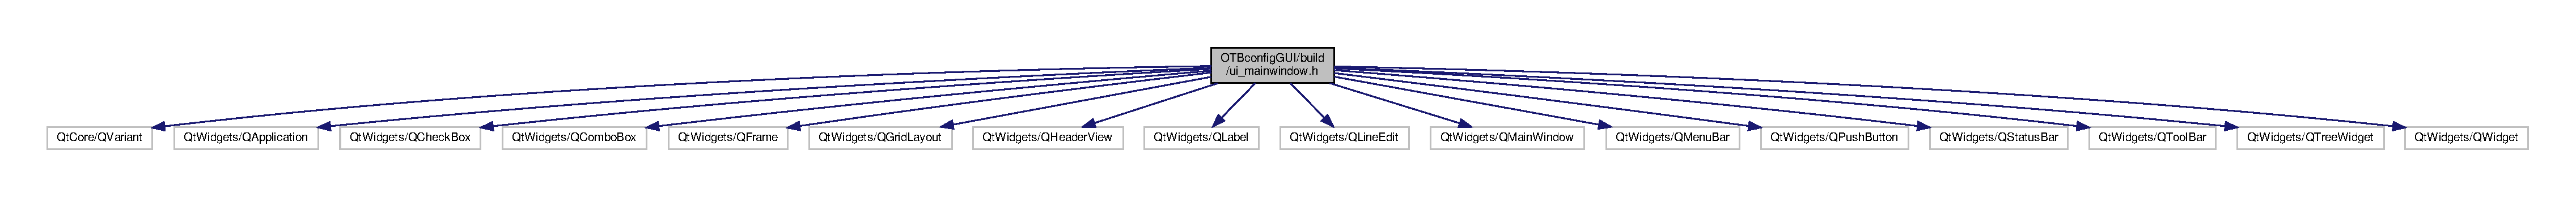
\includegraphics[width=350pt]{d7/dd2/ui__mainwindow_8h__incl}
\end{center}
\end{figure}
This graph shows which files directly or indirectly include this file\+:
\nopagebreak
\begin{figure}[H]
\begin{center}
\leavevmode
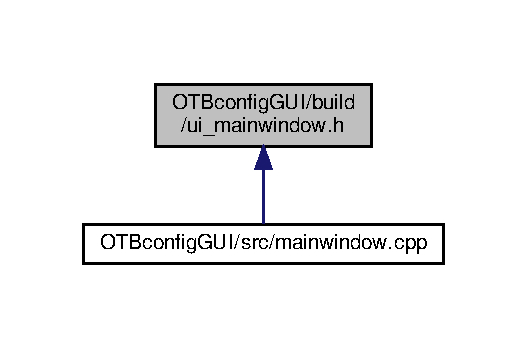
\includegraphics[width=253pt]{d7/d8b/ui__mainwindow_8h__dep__incl}
\end{center}
\end{figure}
\subsection*{Classes}
\begin{DoxyCompactItemize}
\item 
class \hyperlink{class_ui___main_window}{Ui\+\_\+\+Main\+Window}
\item 
class \hyperlink{class_ui_1_1_main_window}{Ui\+::\+Main\+Window}
\end{DoxyCompactItemize}
\subsection*{Namespaces}
\begin{DoxyCompactItemize}
\item 
 \hyperlink{namespace_ui}{Ui}
\end{DoxyCompactItemize}

\hypertarget{mainwindow_8h}{}\section{O\+T\+Bconfig\+G\+U\+I/include/mainwindow.h File Reference}
\label{mainwindow_8h}\index{O\+T\+Bconfig\+G\+U\+I/include/mainwindow.\+h@{O\+T\+Bconfig\+G\+U\+I/include/mainwindow.\+h}}
{\ttfamily \#include $<$Q\+Main\+Window$>$}\newline
Include dependency graph for mainwindow.\+h\+:
\nopagebreak
\begin{figure}[H]
\begin{center}
\leavevmode
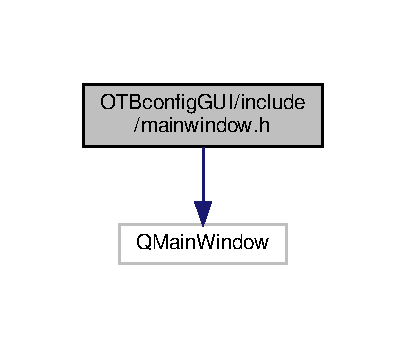
\includegraphics[width=195pt]{d2/d32/mainwindow_8h__incl}
\end{center}
\end{figure}
This graph shows which files directly or indirectly include this file\+:
\nopagebreak
\begin{figure}[H]
\begin{center}
\leavevmode
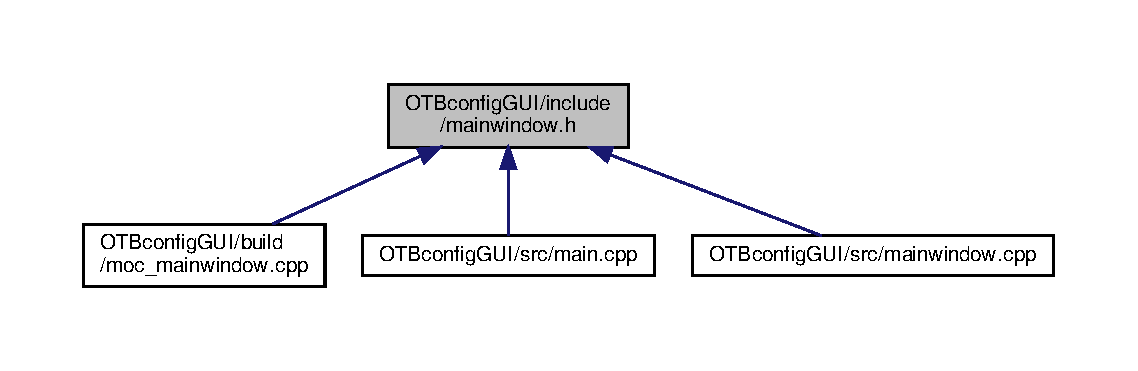
\includegraphics[width=350pt]{dc/d59/mainwindow_8h__dep__incl}
\end{center}
\end{figure}
\subsection*{Classes}
\begin{DoxyCompactItemize}
\item 
class \hyperlink{class_main_window}{Main\+Window}
\end{DoxyCompactItemize}
\subsection*{Namespaces}
\begin{DoxyCompactItemize}
\item 
 \hyperlink{namespace_ui}{Ui}
\end{DoxyCompactItemize}
\subsection*{Macros}
\begin{DoxyCompactItemize}
\item 
\#define \hyperlink{mainwindow_8h_abf8ef69c456ee2c69e0b31bcbbfecf46}{A\+C\+Q\+\_\+\+S\+E\+TT}~0b10000000
\item 
\#define \hyperlink{mainwindow_8h_a76df0c2a7422b57efb6bdafad46eccad}{D\+E\+C\+IM}~0b01000000
\item 
\#define \hyperlink{mainwindow_8h_a0cd1a30341827a0978898092ae67f953}{R\+E\+C\+\_\+\+ON}~0b00100000
\item 
\#define \hyperlink{mainwindow_8h_a9ace2a55b194d5503d72baedea802f68}{F\+S\+A\+M\+P1}~0b00010000
\item 
\#define \hyperlink{mainwindow_8h_afcfb59a63d197f89778038092e9e027d}{F\+S\+A\+M\+P0}~0b00001000
\item 
\#define \hyperlink{mainwindow_8h_ab2c2f4f35a5c9b00875c2ccd35c27918}{N\+C\+H1}~0b00000100
\item 
\#define \hyperlink{mainwindow_8h_ac47c5adaa9e763f6e025ee375c27737e}{N\+C\+H0}~0b00000010
\item 
\#define \hyperlink{mainwindow_8h_a2e5c538236163bd300d8105edc39d080}{A\+C\+Q\+\_\+\+ON}~0b00000001
\item 
\#define \hyperlink{mainwindow_8h_a561caad5df6dc6538cc8937b92ac1cec}{A\+C\+Q\+\_\+\+O\+FF}~0b00000000
\item 
\#define \hyperlink{mainwindow_8h_a690a7565f5c52ec1176048e29c22baae}{C\+R\+C\+\_\+\+C\+O\+DE}~0b10001100
\item 
\#define \hyperlink{mainwindow_8h_aa40c2609604c572c89d9bf1063a0a08b}{C\+O\+N\+F\+I\+G\+\_\+\+S\+I\+ZE}~40
\end{DoxyCompactItemize}


\subsection{Macro Definition Documentation}
\mbox{\Hypertarget{mainwindow_8h_a561caad5df6dc6538cc8937b92ac1cec}\label{mainwindow_8h_a561caad5df6dc6538cc8937b92ac1cec}} 
\index{mainwindow.\+h@{mainwindow.\+h}!A\+C\+Q\+\_\+\+O\+FF@{A\+C\+Q\+\_\+\+O\+FF}}
\index{A\+C\+Q\+\_\+\+O\+FF@{A\+C\+Q\+\_\+\+O\+FF}!mainwindow.\+h@{mainwindow.\+h}}
\subsubsection{\texorpdfstring{A\+C\+Q\+\_\+\+O\+FF}{ACQ\_OFF}}
{\footnotesize\ttfamily \#define A\+C\+Q\+\_\+\+O\+FF~0b00000000}

\mbox{\Hypertarget{mainwindow_8h_a2e5c538236163bd300d8105edc39d080}\label{mainwindow_8h_a2e5c538236163bd300d8105edc39d080}} 
\index{mainwindow.\+h@{mainwindow.\+h}!A\+C\+Q\+\_\+\+ON@{A\+C\+Q\+\_\+\+ON}}
\index{A\+C\+Q\+\_\+\+ON@{A\+C\+Q\+\_\+\+ON}!mainwindow.\+h@{mainwindow.\+h}}
\subsubsection{\texorpdfstring{A\+C\+Q\+\_\+\+ON}{ACQ\_ON}}
{\footnotesize\ttfamily \#define A\+C\+Q\+\_\+\+ON~0b00000001}

\mbox{\Hypertarget{mainwindow_8h_abf8ef69c456ee2c69e0b31bcbbfecf46}\label{mainwindow_8h_abf8ef69c456ee2c69e0b31bcbbfecf46}} 
\index{mainwindow.\+h@{mainwindow.\+h}!A\+C\+Q\+\_\+\+S\+E\+TT@{A\+C\+Q\+\_\+\+S\+E\+TT}}
\index{A\+C\+Q\+\_\+\+S\+E\+TT@{A\+C\+Q\+\_\+\+S\+E\+TT}!mainwindow.\+h@{mainwindow.\+h}}
\subsubsection{\texorpdfstring{A\+C\+Q\+\_\+\+S\+E\+TT}{ACQ\_SETT}}
{\footnotesize\ttfamily \#define A\+C\+Q\+\_\+\+S\+E\+TT~0b10000000}

\mbox{\Hypertarget{mainwindow_8h_aa40c2609604c572c89d9bf1063a0a08b}\label{mainwindow_8h_aa40c2609604c572c89d9bf1063a0a08b}} 
\index{mainwindow.\+h@{mainwindow.\+h}!C\+O\+N\+F\+I\+G\+\_\+\+S\+I\+ZE@{C\+O\+N\+F\+I\+G\+\_\+\+S\+I\+ZE}}
\index{C\+O\+N\+F\+I\+G\+\_\+\+S\+I\+ZE@{C\+O\+N\+F\+I\+G\+\_\+\+S\+I\+ZE}!mainwindow.\+h@{mainwindow.\+h}}
\subsubsection{\texorpdfstring{C\+O\+N\+F\+I\+G\+\_\+\+S\+I\+ZE}{CONFIG\_SIZE}}
{\footnotesize\ttfamily \#define C\+O\+N\+F\+I\+G\+\_\+\+S\+I\+ZE~40}

\mbox{\Hypertarget{mainwindow_8h_a690a7565f5c52ec1176048e29c22baae}\label{mainwindow_8h_a690a7565f5c52ec1176048e29c22baae}} 
\index{mainwindow.\+h@{mainwindow.\+h}!C\+R\+C\+\_\+\+C\+O\+DE@{C\+R\+C\+\_\+\+C\+O\+DE}}
\index{C\+R\+C\+\_\+\+C\+O\+DE@{C\+R\+C\+\_\+\+C\+O\+DE}!mainwindow.\+h@{mainwindow.\+h}}
\subsubsection{\texorpdfstring{C\+R\+C\+\_\+\+C\+O\+DE}{CRC\_CODE}}
{\footnotesize\ttfamily \#define C\+R\+C\+\_\+\+C\+O\+DE~0b10001100}

\mbox{\Hypertarget{mainwindow_8h_a76df0c2a7422b57efb6bdafad46eccad}\label{mainwindow_8h_a76df0c2a7422b57efb6bdafad46eccad}} 
\index{mainwindow.\+h@{mainwindow.\+h}!D\+E\+C\+IM@{D\+E\+C\+IM}}
\index{D\+E\+C\+IM@{D\+E\+C\+IM}!mainwindow.\+h@{mainwindow.\+h}}
\subsubsection{\texorpdfstring{D\+E\+C\+IM}{DECIM}}
{\footnotesize\ttfamily \#define D\+E\+C\+IM~0b01000000}

\mbox{\Hypertarget{mainwindow_8h_afcfb59a63d197f89778038092e9e027d}\label{mainwindow_8h_afcfb59a63d197f89778038092e9e027d}} 
\index{mainwindow.\+h@{mainwindow.\+h}!F\+S\+A\+M\+P0@{F\+S\+A\+M\+P0}}
\index{F\+S\+A\+M\+P0@{F\+S\+A\+M\+P0}!mainwindow.\+h@{mainwindow.\+h}}
\subsubsection{\texorpdfstring{F\+S\+A\+M\+P0}{FSAMP0}}
{\footnotesize\ttfamily \#define F\+S\+A\+M\+P0~0b00001000}

\mbox{\Hypertarget{mainwindow_8h_a9ace2a55b194d5503d72baedea802f68}\label{mainwindow_8h_a9ace2a55b194d5503d72baedea802f68}} 
\index{mainwindow.\+h@{mainwindow.\+h}!F\+S\+A\+M\+P1@{F\+S\+A\+M\+P1}}
\index{F\+S\+A\+M\+P1@{F\+S\+A\+M\+P1}!mainwindow.\+h@{mainwindow.\+h}}
\subsubsection{\texorpdfstring{F\+S\+A\+M\+P1}{FSAMP1}}
{\footnotesize\ttfamily \#define F\+S\+A\+M\+P1~0b00010000}

\mbox{\Hypertarget{mainwindow_8h_ac47c5adaa9e763f6e025ee375c27737e}\label{mainwindow_8h_ac47c5adaa9e763f6e025ee375c27737e}} 
\index{mainwindow.\+h@{mainwindow.\+h}!N\+C\+H0@{N\+C\+H0}}
\index{N\+C\+H0@{N\+C\+H0}!mainwindow.\+h@{mainwindow.\+h}}
\subsubsection{\texorpdfstring{N\+C\+H0}{NCH0}}
{\footnotesize\ttfamily \#define N\+C\+H0~0b00000010}

\mbox{\Hypertarget{mainwindow_8h_ab2c2f4f35a5c9b00875c2ccd35c27918}\label{mainwindow_8h_ab2c2f4f35a5c9b00875c2ccd35c27918}} 
\index{mainwindow.\+h@{mainwindow.\+h}!N\+C\+H1@{N\+C\+H1}}
\index{N\+C\+H1@{N\+C\+H1}!mainwindow.\+h@{mainwindow.\+h}}
\subsubsection{\texorpdfstring{N\+C\+H1}{NCH1}}
{\footnotesize\ttfamily \#define N\+C\+H1~0b00000100}

\mbox{\Hypertarget{mainwindow_8h_a0cd1a30341827a0978898092ae67f953}\label{mainwindow_8h_a0cd1a30341827a0978898092ae67f953}} 
\index{mainwindow.\+h@{mainwindow.\+h}!R\+E\+C\+\_\+\+ON@{R\+E\+C\+\_\+\+ON}}
\index{R\+E\+C\+\_\+\+ON@{R\+E\+C\+\_\+\+ON}!mainwindow.\+h@{mainwindow.\+h}}
\subsubsection{\texorpdfstring{R\+E\+C\+\_\+\+ON}{REC\_ON}}
{\footnotesize\ttfamily \#define R\+E\+C\+\_\+\+ON~0b00100000}


\hypertarget{_o_t_bconfig_g_u_i_2_r_e_a_d_m_e_8md}{}\section{O\+T\+Bconfig\+G\+U\+I/\+R\+E\+A\+D\+ME.md File Reference}
\label{_o_t_bconfig_g_u_i_2_r_e_a_d_m_e_8md}\index{O\+T\+Bconfig\+G\+U\+I/\+R\+E\+A\+D\+M\+E.\+md@{O\+T\+Bconfig\+G\+U\+I/\+R\+E\+A\+D\+M\+E.\+md}}

\hypertarget{_r_e_a_d_m_e_8md}{}\section{R\+E\+A\+D\+M\+E.\+md File Reference}
\label{_r_e_a_d_m_e_8md}\index{R\+E\+A\+D\+M\+E.\+md@{R\+E\+A\+D\+M\+E.\+md}}

\hypertarget{_o_t_bconfig_g_u_i_2src_2main_8cpp}{}\section{O\+T\+Bconfig\+G\+U\+I/src/main.cpp File Reference}
\label{_o_t_bconfig_g_u_i_2src_2main_8cpp}\index{O\+T\+Bconfig\+G\+U\+I/src/main.\+cpp@{O\+T\+Bconfig\+G\+U\+I/src/main.\+cpp}}
{\ttfamily \#include \char`\"{}mainwindow.\+h\char`\"{}}\newline
{\ttfamily \#include $<$Q\+Application$>$}\newline
Include dependency graph for main.\+cpp\+:
\nopagebreak
\begin{figure}[H]
\begin{center}
\leavevmode
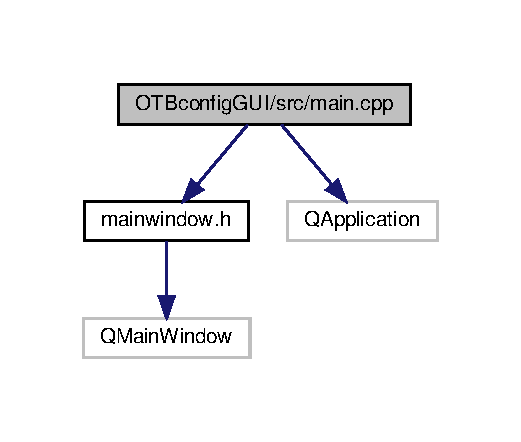
\includegraphics[width=250pt]{d3/d40/_o_t_bconfig_g_u_i_2src_2main_8cpp__incl}
\end{center}
\end{figure}
\subsection*{Functions}
\begin{DoxyCompactItemize}
\item 
int \hyperlink{_o_t_bconfig_g_u_i_2src_2main_8cpp_a0ddf1224851353fc92bfbff6f499fa97}{main} (int argc, char $\ast$argv\mbox{[}$\,$\mbox{]})
\end{DoxyCompactItemize}


\subsection{Function Documentation}
\mbox{\Hypertarget{_o_t_bconfig_g_u_i_2src_2main_8cpp_a0ddf1224851353fc92bfbff6f499fa97}\label{_o_t_bconfig_g_u_i_2src_2main_8cpp_a0ddf1224851353fc92bfbff6f499fa97}} 
\index{O\+T\+Bconfig\+G\+U\+I/src/main.\+cpp@{O\+T\+Bconfig\+G\+U\+I/src/main.\+cpp}!main@{main}}
\index{main@{main}!O\+T\+Bconfig\+G\+U\+I/src/main.\+cpp@{O\+T\+Bconfig\+G\+U\+I/src/main.\+cpp}}
\subsubsection{\texorpdfstring{main()}{main()}}
{\footnotesize\ttfamily int main (\begin{DoxyParamCaption}\item[{int}]{argc,  }\item[{char $\ast$}]{argv\mbox{[}$\,$\mbox{]} }\end{DoxyParamCaption})}


\hypertarget{src_2main_8cpp}{}\section{src/main.cpp File Reference}
\label{src_2main_8cpp}\index{src/main.\+cpp@{src/main.\+cpp}}
{\ttfamily \#include $<$vector$>$}\newline
{\ttfamily \#include $<$fstream$>$}\newline
{\ttfamily \#include $<$iostream$>$}\newline
{\ttfamily \#include $<$lsl\+\_\+cpp.\+h$>$}\newline
{\ttfamily \#include \char`\"{}O\+T\+Bconfig.\+h\char`\"{}}\newline
{\ttfamily \#include \char`\"{}tools.\+h\char`\"{}}\newline
Include dependency graph for main.\+cpp\+:
\nopagebreak
\begin{figure}[H]
\begin{center}
\leavevmode
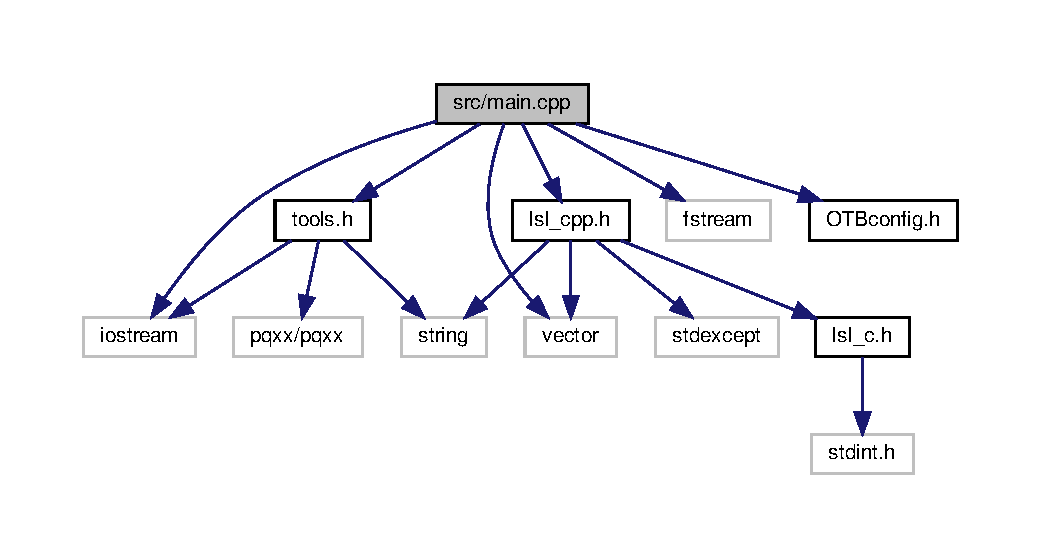
\includegraphics[width=350pt]{da/dfa/src_2main_8cpp__incl}
\end{center}
\end{figure}
\subsection*{Macros}
\begin{DoxyCompactItemize}
\item 
\#define \hyperlink{src_2main_8cpp_a282b5ca7d691d6a8ca66c15a0fc0707b}{S\+A\+M\+P\+L\+I\+N\+G\+\_\+\+F\+R\+E\+Q\+U\+E\+N\+CY}~2048
\item 
\#define \hyperlink{src_2main_8cpp_aea3cfda4f3a9f978ec759f206cf186fe}{C\+H\+U\+N\+K\+\_\+\+S\+I\+ZE}~1
\end{DoxyCompactItemize}
\subsection*{Functions}
\begin{DoxyCompactItemize}
\item 
{\footnotesize template$<$class T $>$ }\\void \hyperlink{src_2main_8cpp_ab63fc66f6d459b5934771a5236ba062a}{fill\+\_\+chunk} (unsigned char $\ast$from, std\+::vector$<$ std\+::vector$<$ T $>$$>$ \&to, int nb\+\_\+ch, int n=\hyperlink{src_2main_8cpp_aea3cfda4f3a9f978ec759f206cf186fe}{C\+H\+U\+N\+K\+\_\+\+S\+I\+ZE})
\begin{DoxyCompactList}\small\item\em fill\+\_\+chunk transform a unsigned char array into a typed vector of vector. \end{DoxyCompactList}\item 
void \hyperlink{src_2main_8cpp_ac69b13801e31a93d47c62194924d0af8}{get\+Conf} (std\+::string path, unsigned char $\ast$config)
\begin{DoxyCompactList}\small\item\em fill\+\_\+chunk transform a unsigned char array into a typed vector of vector. \end{DoxyCompactList}\item 
int \hyperlink{src_2main_8cpp_ab0977b25f5ebf5c2fe484d875330b745}{get\+\_\+sampling\+\_\+rate} (unsigned char $\ast$config)
\begin{DoxyCompactList}\small\item\em get\+\_\+sampling\+\_\+rate Get and interpret the sampling frequency bites of the config array and return the coresponding rate. \end{DoxyCompactList}\item 
int \hyperlink{src_2main_8cpp_aa3eb305d2f10786be43b75e75bc19f95}{get\+\_\+nb\+Channels} (unsigned char $\ast$config)
\begin{DoxyCompactList}\small\item\em get\+\_\+sampling\+\_\+rate Get and interpret the number of channels bites of the config array and return the coresponding rate \end{DoxyCompactList}\item 
int \hyperlink{src_2main_8cpp_a3c04138a5bfe5d72780bb7e82a18e627}{main} (int argc, char $\ast$$\ast$argv)
\end{DoxyCompactItemize}


\subsection{Macro Definition Documentation}
\mbox{\Hypertarget{src_2main_8cpp_aea3cfda4f3a9f978ec759f206cf186fe}\label{src_2main_8cpp_aea3cfda4f3a9f978ec759f206cf186fe}} 
\index{src/main.\+cpp@{src/main.\+cpp}!C\+H\+U\+N\+K\+\_\+\+S\+I\+ZE@{C\+H\+U\+N\+K\+\_\+\+S\+I\+ZE}}
\index{C\+H\+U\+N\+K\+\_\+\+S\+I\+ZE@{C\+H\+U\+N\+K\+\_\+\+S\+I\+ZE}!src/main.\+cpp@{src/main.\+cpp}}
\subsubsection{\texorpdfstring{C\+H\+U\+N\+K\+\_\+\+S\+I\+ZE}{CHUNK\_SIZE}}
{\footnotesize\ttfamily \#define C\+H\+U\+N\+K\+\_\+\+S\+I\+ZE~1}

\mbox{\Hypertarget{src_2main_8cpp_a282b5ca7d691d6a8ca66c15a0fc0707b}\label{src_2main_8cpp_a282b5ca7d691d6a8ca66c15a0fc0707b}} 
\index{src/main.\+cpp@{src/main.\+cpp}!S\+A\+M\+P\+L\+I\+N\+G\+\_\+\+F\+R\+E\+Q\+U\+E\+N\+CY@{S\+A\+M\+P\+L\+I\+N\+G\+\_\+\+F\+R\+E\+Q\+U\+E\+N\+CY}}
\index{S\+A\+M\+P\+L\+I\+N\+G\+\_\+\+F\+R\+E\+Q\+U\+E\+N\+CY@{S\+A\+M\+P\+L\+I\+N\+G\+\_\+\+F\+R\+E\+Q\+U\+E\+N\+CY}!src/main.\+cpp@{src/main.\+cpp}}
\subsubsection{\texorpdfstring{S\+A\+M\+P\+L\+I\+N\+G\+\_\+\+F\+R\+E\+Q\+U\+E\+N\+CY}{SAMPLING\_FREQUENCY}}
{\footnotesize\ttfamily \#define S\+A\+M\+P\+L\+I\+N\+G\+\_\+\+F\+R\+E\+Q\+U\+E\+N\+CY~2048}



\subsection{Function Documentation}
\mbox{\Hypertarget{src_2main_8cpp_ab63fc66f6d459b5934771a5236ba062a}\label{src_2main_8cpp_ab63fc66f6d459b5934771a5236ba062a}} 
\index{src/main.\+cpp@{src/main.\+cpp}!fill\+\_\+chunk@{fill\+\_\+chunk}}
\index{fill\+\_\+chunk@{fill\+\_\+chunk}!src/main.\+cpp@{src/main.\+cpp}}
\subsubsection{\texorpdfstring{fill\+\_\+chunk()}{fill\_chunk()}}
{\footnotesize\ttfamily template$<$class T $>$ \\
void fill\+\_\+chunk (\begin{DoxyParamCaption}\item[{unsigned char $\ast$}]{from,  }\item[{std\+::vector$<$ std\+::vector$<$ T $>$$>$ \&}]{to,  }\item[{int}]{nb\+\_\+ch,  }\item[{int}]{n = {\ttfamily \hyperlink{src_2main_8cpp_aea3cfda4f3a9f978ec759f206cf186fe}{C\+H\+U\+N\+K\+\_\+\+S\+I\+ZE}} }\end{DoxyParamCaption})}



fill\+\_\+chunk transform a unsigned char array into a typed vector of vector. 


\begin{DoxyTemplParams}{Template Parameters}
{\em T} & Type of the vector. \\
\hline
\end{DoxyTemplParams}

\begin{DoxyParams}{Parameters}
{\em from} & Unsigned char array to transform. \\
\hline
{\em to} & Resulting vector of vector of type T. \\
\hline
{\em nb\+\_\+ch} & Number of channel of the stream. \\
\hline
{\em n} & Number of sample in the array. \\
\hline
\end{DoxyParams}
\mbox{\Hypertarget{src_2main_8cpp_aa3eb305d2f10786be43b75e75bc19f95}\label{src_2main_8cpp_aa3eb305d2f10786be43b75e75bc19f95}} 
\index{src/main.\+cpp@{src/main.\+cpp}!get\+\_\+nb\+Channels@{get\+\_\+nb\+Channels}}
\index{get\+\_\+nb\+Channels@{get\+\_\+nb\+Channels}!src/main.\+cpp@{src/main.\+cpp}}
\subsubsection{\texorpdfstring{get\+\_\+nb\+Channels()}{get\_nbChannels()}}
{\footnotesize\ttfamily int get\+\_\+nb\+Channels (\begin{DoxyParamCaption}\item[{unsigned char $\ast$}]{config }\end{DoxyParamCaption})}



get\+\_\+sampling\+\_\+rate Get and interpret the number of channels bites of the config array and return the coresponding rate 


\begin{DoxyParams}{Parameters}
{\em config} & The configuration array used in the program. \\
\hline
\end{DoxyParams}
\mbox{\Hypertarget{src_2main_8cpp_ab0977b25f5ebf5c2fe484d875330b745}\label{src_2main_8cpp_ab0977b25f5ebf5c2fe484d875330b745}} 
\index{src/main.\+cpp@{src/main.\+cpp}!get\+\_\+sampling\+\_\+rate@{get\+\_\+sampling\+\_\+rate}}
\index{get\+\_\+sampling\+\_\+rate@{get\+\_\+sampling\+\_\+rate}!src/main.\+cpp@{src/main.\+cpp}}
\subsubsection{\texorpdfstring{get\+\_\+sampling\+\_\+rate()}{get\_sampling\_rate()}}
{\footnotesize\ttfamily int get\+\_\+sampling\+\_\+rate (\begin{DoxyParamCaption}\item[{unsigned char $\ast$}]{config }\end{DoxyParamCaption})}



get\+\_\+sampling\+\_\+rate Get and interpret the sampling frequency bites of the config array and return the coresponding rate. 


\begin{DoxyParams}{Parameters}
{\em config} & The configuration array used in the program. \\
\hline
\end{DoxyParams}
\mbox{\Hypertarget{src_2main_8cpp_ac69b13801e31a93d47c62194924d0af8}\label{src_2main_8cpp_ac69b13801e31a93d47c62194924d0af8}} 
\index{src/main.\+cpp@{src/main.\+cpp}!get\+Conf@{get\+Conf}}
\index{get\+Conf@{get\+Conf}!src/main.\+cpp@{src/main.\+cpp}}
\subsubsection{\texorpdfstring{get\+Conf()}{getConf()}}
{\footnotesize\ttfamily void get\+Conf (\begin{DoxyParamCaption}\item[{std\+::string}]{path,  }\item[{unsigned char $\ast$}]{config }\end{DoxyParamCaption})}



fill\+\_\+chunk transform a unsigned char array into a typed vector of vector. 


\begin{DoxyParams}{Parameters}
{\em path} & Path of the configuration file.. \\
\hline
{\em config} & The configuration array used in the program. \\
\hline
\end{DoxyParams}
\mbox{\Hypertarget{src_2main_8cpp_a3c04138a5bfe5d72780bb7e82a18e627}\label{src_2main_8cpp_a3c04138a5bfe5d72780bb7e82a18e627}} 
\index{src/main.\+cpp@{src/main.\+cpp}!main@{main}}
\index{main@{main}!src/main.\+cpp@{src/main.\+cpp}}
\subsubsection{\texorpdfstring{main()}{main()}}
{\footnotesize\ttfamily int main (\begin{DoxyParamCaption}\item[{int}]{argc,  }\item[{char $\ast$$\ast$}]{argv }\end{DoxyParamCaption})}


\hypertarget{mainwindow_8cpp}{}\section{O\+T\+Bconfig\+G\+U\+I/src/mainwindow.cpp File Reference}
\label{mainwindow_8cpp}\index{O\+T\+Bconfig\+G\+U\+I/src/mainwindow.\+cpp@{O\+T\+Bconfig\+G\+U\+I/src/mainwindow.\+cpp}}
{\ttfamily \#include \char`\"{}mainwindow.\+h\char`\"{}}\newline
{\ttfamily \#include \char`\"{}ui\+\_\+mainwindow.\+h\char`\"{}}\newline
{\ttfamily \#include $<$Q\+Tree\+Widget$>$}\newline
{\ttfamily \#include $<$fstream$>$}\newline
{\ttfamily \#include $<$iostream$>$}\newline
Include dependency graph for mainwindow.\+cpp\+:
\nopagebreak
\begin{figure}[H]
\begin{center}
\leavevmode
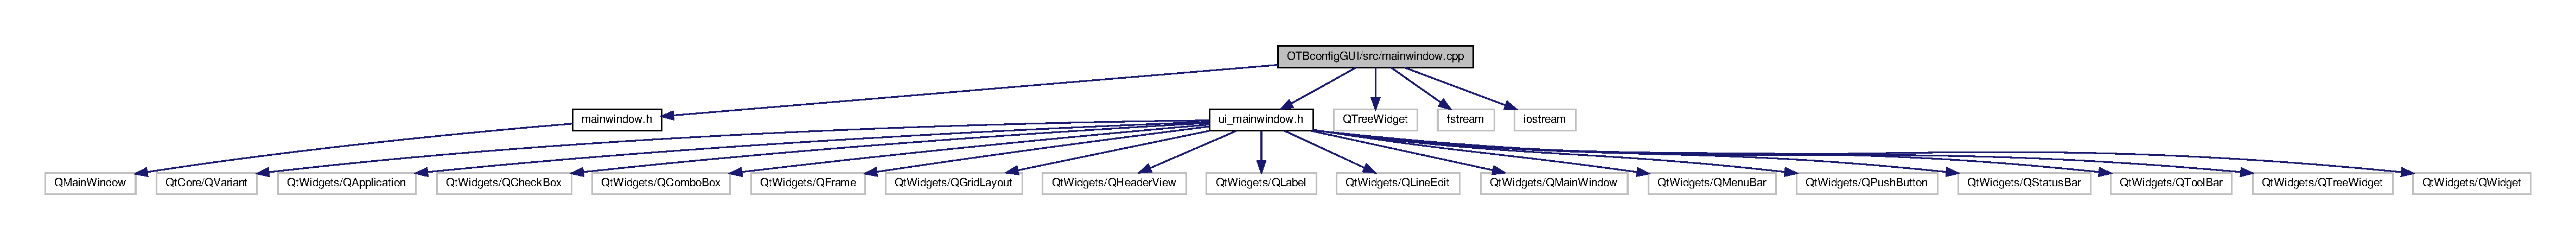
\includegraphics[width=350pt]{d1/dd5/mainwindow_8cpp__incl}
\end{center}
\end{figure}

\hypertarget{_o_t_bconfig_8cpp}{}\section{src/\+O\+T\+Bconfig.cpp File Reference}
\label{_o_t_bconfig_8cpp}\index{src/\+O\+T\+Bconfig.\+cpp@{src/\+O\+T\+Bconfig.\+cpp}}
{\ttfamily \#include \char`\"{}O\+T\+Bconfig.\+h\char`\"{}}\newline
{\ttfamily \#include $<$iostream$>$}\newline
Include dependency graph for O\+T\+Bconfig.\+cpp\+:
\nopagebreak
\begin{figure}[H]
\begin{center}
\leavevmode
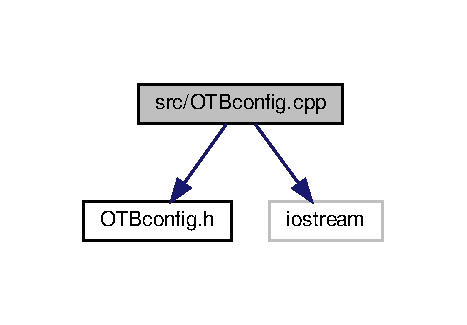
\includegraphics[width=224pt]{db/db0/_o_t_bconfig_8cpp__incl}
\end{center}
\end{figure}
\subsection*{Functions}
\begin{DoxyCompactItemize}
\item 
unsigned char \hyperlink{_o_t_bconfig_8cpp_a0596e4e702611a9eb9b7944b5e8d2052}{crc} (unsigned char config\mbox{[}$\,$\mbox{]})
\item 
void \hyperlink{_o_t_bconfig_8cpp_adb228c7505a0533deaff911c6f2052e6}{print\+B\+IN} (char n)
\end{DoxyCompactItemize}


\subsection{Function Documentation}
\mbox{\Hypertarget{_o_t_bconfig_8cpp_a0596e4e702611a9eb9b7944b5e8d2052}\label{_o_t_bconfig_8cpp_a0596e4e702611a9eb9b7944b5e8d2052}} 
\index{O\+T\+Bconfig.\+cpp@{O\+T\+Bconfig.\+cpp}!crc@{crc}}
\index{crc@{crc}!O\+T\+Bconfig.\+cpp@{O\+T\+Bconfig.\+cpp}}
\subsubsection{\texorpdfstring{crc()}{crc()}}
{\footnotesize\ttfamily unsigned char crc (\begin{DoxyParamCaption}\item[{unsigned char}]{config\mbox{[}$\,$\mbox{]} }\end{DoxyParamCaption})}

\mbox{\Hypertarget{_o_t_bconfig_8cpp_adb228c7505a0533deaff911c6f2052e6}\label{_o_t_bconfig_8cpp_adb228c7505a0533deaff911c6f2052e6}} 
\index{O\+T\+Bconfig.\+cpp@{O\+T\+Bconfig.\+cpp}!print\+B\+IN@{print\+B\+IN}}
\index{print\+B\+IN@{print\+B\+IN}!O\+T\+Bconfig.\+cpp@{O\+T\+Bconfig.\+cpp}}
\subsubsection{\texorpdfstring{print\+B\+I\+N()}{printBIN()}}
{\footnotesize\ttfamily void print\+B\+IN (\begin{DoxyParamCaption}\item[{char}]{n }\end{DoxyParamCaption})}


\hypertarget{tools_8cpp}{}\section{src/tools.cpp File Reference}
\label{tools_8cpp}\index{src/tools.\+cpp@{src/tools.\+cpp}}


T\+O\+DO.  


{\ttfamily \#include \char`\"{}tools.\+h\char`\"{}}\newline
Include dependency graph for tools.\+cpp\+:\nopagebreak
\begin{figure}[H]
\begin{center}
\leavevmode
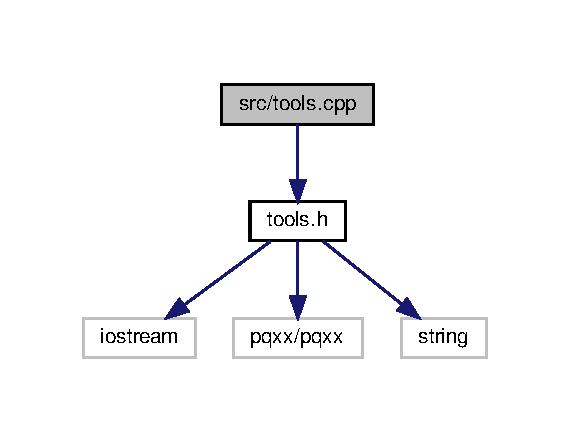
\includegraphics[width=274pt]{d1/d1f/tools_8cpp__incl}
\end{center}
\end{figure}
\subsection*{Functions}
\begin{DoxyCompactItemize}
\item 
void \hyperlink{tools_8cpp_a61c5db3de2e3870f15756d0ad8440990}{error} (std\+::string str)
\begin{DoxyCompactList}\small\item\em error Display the passed string thne exit the program. \end{DoxyCompactList}\item 
void \hyperlink{tools_8cpp_a91602e2ffffd88f2b5f4280ef0d9e3be}{usage} (std\+::vector$<$ std\+::string $>$ \&optf, std\+::vector$<$ std\+::string $>$ \&optl, std\+::vector$<$ std\+::string $>$ \&optv)
\begin{DoxyCompactList}\small\item\em usage Display the usage, then exit the program. \end{DoxyCompactList}\item 
void \hyperlink{tools_8cpp_afc65291b27e568d76cf11518d7c2123e}{get\+\_\+arg} (int argc, char $\ast$$\ast$argv, std\+::vector$<$ std\+::string $>$ \&optf, std\+::vector$<$ std\+::string $>$ \&optl, std\+::vector$<$ std\+::string $>$ \&optv)
\begin{DoxyCompactList}\small\item\em get\+\_\+arg Search for the potential argument in the argument passed to the program. \end{DoxyCompactList}\end{DoxyCompactItemize}


\subsection{Detailed Description}
T\+O\+DO. 

\begin{DoxyAuthor}{Author}
Alexis Devillard 
\end{DoxyAuthor}
\begin{DoxyVersion}{Version}
1.\+0 
\end{DoxyVersion}
\begin{DoxyDate}{Date}
08 may 2019 
\end{DoxyDate}


\subsection{Function Documentation}
\mbox{\Hypertarget{tools_8cpp_a61c5db3de2e3870f15756d0ad8440990}\label{tools_8cpp_a61c5db3de2e3870f15756d0ad8440990}} 
\index{tools.\+cpp@{tools.\+cpp}!error@{error}}
\index{error@{error}!tools.\+cpp@{tools.\+cpp}}
\subsubsection{\texorpdfstring{error()}{error()}}
{\footnotesize\ttfamily void error (\begin{DoxyParamCaption}\item[{std\+::string}]{str }\end{DoxyParamCaption})}



error Display the passed string thne exit the program. 


\begin{DoxyParams}{Parameters}
{\em str} & String to display. \\
\hline
\end{DoxyParams}
\mbox{\Hypertarget{tools_8cpp_afc65291b27e568d76cf11518d7c2123e}\label{tools_8cpp_afc65291b27e568d76cf11518d7c2123e}} 
\index{tools.\+cpp@{tools.\+cpp}!get\+\_\+arg@{get\+\_\+arg}}
\index{get\+\_\+arg@{get\+\_\+arg}!tools.\+cpp@{tools.\+cpp}}
\subsubsection{\texorpdfstring{get\+\_\+arg()}{get\_arg()}}
{\footnotesize\ttfamily void get\+\_\+arg (\begin{DoxyParamCaption}\item[{int}]{argc,  }\item[{char $\ast$$\ast$}]{argv,  }\item[{std\+::vector$<$ std\+::string $>$ \&}]{optf,  }\item[{std\+::vector$<$ std\+::string $>$ \&}]{optl,  }\item[{std\+::vector$<$ std\+::string $>$ \&}]{optv }\end{DoxyParamCaption})}



get\+\_\+arg Search for the potential argument in the argument passed to the program. 


\begin{DoxyParams}{Parameters}
{\em argc} & Argument counter \\
\hline
{\em argv} & Argument array \\
\hline
{\em optf} & List of option flags \\
\hline
{\em optf} & List of option labels \\
\hline
{\em optf} & List of option values \\
\hline
\end{DoxyParams}
\mbox{\Hypertarget{tools_8cpp_a91602e2ffffd88f2b5f4280ef0d9e3be}\label{tools_8cpp_a91602e2ffffd88f2b5f4280ef0d9e3be}} 
\index{tools.\+cpp@{tools.\+cpp}!usage@{usage}}
\index{usage@{usage}!tools.\+cpp@{tools.\+cpp}}
\subsubsection{\texorpdfstring{usage()}{usage()}}
{\footnotesize\ttfamily void usage (\begin{DoxyParamCaption}\item[{std\+::vector$<$ std\+::string $>$ \&}]{optf,  }\item[{std\+::vector$<$ std\+::string $>$ \&}]{optl,  }\item[{std\+::vector$<$ std\+::string $>$ \&}]{optv }\end{DoxyParamCaption})}



usage Display the usage, then exit the program. 


\begin{DoxyParams}{Parameters}
{\em optf} & List of option flags \\
\hline
{\em optf} & List of option labels \\
\hline
{\em optf} & List of option values \\
\hline
\end{DoxyParams}

%--- End generated contents ---

% Index
\backmatter
\newpage
\phantomsection
\clearemptydoublepage
\addcontentsline{toc}{chapter}{Index}
\printindex

\end{document}
